\documentclass[twoside]{book}

% Packages required by doxygen
\usepackage{fixltx2e}
\usepackage{calc}
\usepackage{doxygen}
\usepackage[export]{adjustbox} % also loads graphicx
\usepackage{graphicx}
\usepackage[utf8]{inputenc}
\usepackage{makeidx}
\usepackage{multicol}
\usepackage{multirow}
\PassOptionsToPackage{warn}{textcomp}
\usepackage{textcomp}
\usepackage[nointegrals]{wasysym}
\usepackage[table]{xcolor}

% Font selection
\usepackage[T1]{fontenc}
\usepackage[scaled=.90]{helvet}
\usepackage{courier}
\usepackage{amssymb}
\usepackage{sectsty}
\renewcommand{\familydefault}{\sfdefault}
\allsectionsfont{%
  \fontseries{bc}\selectfont%
  \color{darkgray}%
}
\renewcommand{\DoxyLabelFont}{%
  \fontseries{bc}\selectfont%
  \color{darkgray}%
}
\newcommand{\+}{\discretionary{\mbox{\scriptsize$\hookleftarrow$}}{}{}}

% Page & text layout
\usepackage{geometry}
\geometry{%
  a4paper,%
  top=2.5cm,%
  bottom=2.5cm,%
  left=2.5cm,%
  right=2.5cm%
}
\tolerance=750
\hfuzz=15pt
\hbadness=750
\setlength{\emergencystretch}{15pt}
\setlength{\parindent}{0cm}
\setlength{\parskip}{3ex plus 2ex minus 2ex}
\makeatletter
\renewcommand{\paragraph}{%
  \@startsection{paragraph}{4}{0ex}{-1.0ex}{1.0ex}{%
    \normalfont\normalsize\bfseries\SS@parafont%
  }%
}
\renewcommand{\subparagraph}{%
  \@startsection{subparagraph}{5}{0ex}{-1.0ex}{1.0ex}{%
    \normalfont\normalsize\bfseries\SS@subparafont%
  }%
}
\makeatother

% Headers & footers
\usepackage{fancyhdr}
\pagestyle{fancyplain}
\fancyhead[LE]{\fancyplain{}{\bfseries\thepage}}
\fancyhead[CE]{\fancyplain{}{}}
\fancyhead[RE]{\fancyplain{}{\bfseries\leftmark}}
\fancyhead[LO]{\fancyplain{}{\bfseries\rightmark}}
\fancyhead[CO]{\fancyplain{}{}}
\fancyhead[RO]{\fancyplain{}{\bfseries\thepage}}
\fancyfoot[LE]{\fancyplain{}{}}
\fancyfoot[CE]{\fancyplain{}{}}
\fancyfoot[RE]{\fancyplain{}{\bfseries\scriptsize Generated by Doxygen }}
\fancyfoot[LO]{\fancyplain{}{\bfseries\scriptsize Generated by Doxygen }}
\fancyfoot[CO]{\fancyplain{}{}}
\fancyfoot[RO]{\fancyplain{}{}}
\renewcommand{\footrulewidth}{0.4pt}
\renewcommand{\chaptermark}[1]{%
  \markboth{#1}{}%
}
\renewcommand{\sectionmark}[1]{%
  \markright{\thesection\ #1}%
}

% Indices & bibliography
\usepackage{natbib}
\usepackage[titles]{tocloft}
\setcounter{tocdepth}{3}
\setcounter{secnumdepth}{5}
\makeindex

% Hyperlinks (required, but should be loaded last)
\usepackage{ifpdf}
\ifpdf
  \usepackage[pdftex,pagebackref=true]{hyperref}
\else
  \usepackage[ps2pdf,pagebackref=true]{hyperref}
\fi
\hypersetup{%
  colorlinks=true,%
  linkcolor=blue,%
  citecolor=blue,%
  unicode%
}

% Custom commands
\newcommand{\clearemptydoublepage}{%
  \newpage{\pagestyle{empty}\cleardoublepage}%
}

\usepackage{caption}
\captionsetup{labelsep=space,justification=centering,font={bf},singlelinecheck=off,skip=4pt,position=top}

%===== C O N T E N T S =====

\begin{document}

% Titlepage & ToC
\hypersetup{pageanchor=false,
             bookmarksnumbered=true,
             pdfencoding=unicode
            }
\pagenumbering{alph}
\begin{titlepage}
\vspace*{7cm}
\begin{center}%
{\Large Bridges-\/\+C++ \\[1ex]\large 3.\+2.\+0 }\\
\vspace*{1cm}
{\large Generated by Doxygen 1.8.13}\\
\end{center}
\end{titlepage}
\clearemptydoublepage
\pagenumbering{roman}
\tableofcontents
\clearemptydoublepage
\pagenumbering{arabic}
\hypersetup{pageanchor=true}

%--- Begin generated contents ---
\chapter{B\+R\+I\+D\+G\+ES}
\label{index}\hypertarget{index}{}\hypertarget{index_overview_sec}{}\section{Overview}\label{index_overview_sec}
The Bridging Real-\/world Infrastructure Designed to Goal-\/align, Engage, and Stimulate (B\+R\+I\+D\+G\+ES) project is directed at improving the retention of sophomore students in Computer Science by (1) introducing real-\/world datasets (Facebook, Twitter, etc) into course projects involving computer science data structures, and (2) facilitating peer mentoring of sophomores by senior CS students in shared lab experiences that involve the use of the B\+R\+I\+D\+G\+ES infrastructure in software development. \hypertarget{index_br_client}{}\section{B\+R\+I\+D\+G\+E\+S Client Design}\label{index_br_client}
B\+R\+I\+D\+G\+ES client side design loosely follows the basic data structure elements implemented and described in ``A Practical Introduction to Data Structures and Algorithm Analysis" by C.\+A. Shaffer (\href{http://people.cs.vt.edu/shaffer/Book/}{\tt http\+://people.\+cs.\+vt.\+edu/shaffer/\+Book/}). These elements are augmented to contain visual properties that are controlled by the user to customize the visual representation of the constructed data structure. Once a a data structure is ready to be visualized, related B\+R\+I\+D\+G\+ES server calls are made to send a reprsentation of the data structure to B\+R\+I\+D\+G\+ES server. \hypertarget{index_br_server}{}\section{B\+R\+I\+D\+G\+E\+S Server Design.}\label{index_br_server}
B\+R\+I\+D\+G\+ES server implements a combination of technologies (Mongo\+DB, Node, d3\+J\+S(visualization) to receive a data structure representation for visualization. These are largely transparent to the user and involves the user being directed to a web page for viewing the data structure. Attention has been paid to provide meaningful error messages to the user in case problems are encountered in the process. \hypertarget{index_api_sec}{}\section{A\+P\+I Descriptions.}\label{index_api_sec}
See the accompanying pages for detailed description of the B\+R\+I\+D\+G\+ES classes \hypertarget{index_sponsor_sec}{}\subsection{Sponsorship/\+Funding.}\label{index_sponsor_sec}
B\+R\+I\+D\+G\+ES is an N\+SF T\+U\+ES Project.\hypertarget{index_contacts_sec}{}\section{Contacts\+:}\label{index_contacts_sec}
Kalpathi Subramanian, \href{mailto:krs@uncc.edu}{\tt krs@uncc.\+edu}, Jamie Payton, \href{mailto:payton@uncc.edu}{\tt payton@uncc.\+edu}, Michael Youngblood, \href{mailto:gmyoungblood@gmail.com}{\tt gmyoungblood@gmail.\+com}, Robert Kosara, \href{mailto:rkosara@tableau.com}{\tt rkosara@tableau.\+com}

Department of Computer Science, The University of North Carolina at Charlotte, Charlotte, NC. 
\chapter{Namespace Index}
\section{Namespace List}
Here is a list of all namespaces with brief descriptions\+:\begin{DoxyCompactList}
\item\contentsline{section}{\hyperlink{namespacebridges}{bridges} \\*This class can be used to create arrays of type Element$<$\+E$>$ where E is a generic type representation application specific data. Arrays are internally represented as 1\+D arrays; currently 1\+D, 2\+D and 3\+D arrays are supported }{\pageref{namespacebridges}}{}
\item\contentsline{section}{\hyperlink{namespacebridges_1_1base64}{bridges\+::base64} }{\pageref{namespacebridges_1_1base64}}{}
\item\contentsline{section}{\hyperlink{namespacebridges_1_1_j_s_o_n_util}{bridges\+::\+J\+S\+O\+N\+Util} }{\pageref{namespacebridges_1_1_j_s_o_n_util}}{}
\end{DoxyCompactList}

\chapter{Hierarchical Index}
\section{Class Hierarchy}
This inheritance list is sorted roughly, but not completely, alphabetically\+:\begin{DoxyCompactList}
\item \contentsline{section}{bridges\+:\+:dataset\+:\+:Actor\+Movie\+I\+M\+DB}{\pageref{classbridges_1_1dataset_1_1_actor_movie_i_m_d_b}}{}
\item \contentsline{section}{Audio\+Channel}{\pageref{class_audio_channel}}{}
\item \contentsline{section}{bridges\+:\+:dataset\+:\+:Book}{\pageref{classbridges_1_1dataset_1_1_book}}{}
\item \contentsline{section}{bridges\+:\+:datastructure\+:\+:Array3D$<$ E $>$\+:\+:Bracket\+\_\+helper}{\pageref{structbridges_1_1datastructure_1_1_array3_d_1_1_bracket__helper}}{}
\item \contentsline{section}{bridges\+:\+:datastructure\+:\+:Array2D$<$ E $>$\+:\+:Bracket\+\_\+helper}{\pageref{structbridges_1_1datastructure_1_1_array2_d_1_1_bracket__helper}}{}
\item \contentsline{section}{bridges\+:\+:datastructure\+:\+:Array3D$<$ E $>$\+:\+:Bracket\+\_\+helper2}{\pageref{structbridges_1_1datastructure_1_1_array3_d_1_1_bracket__helper2}}{}
\item \contentsline{section}{bridges\+:\+:datastructure\+:\+:Array3D$<$ E $>$\+:\+:Bracket\+\_\+helper2\+\_\+const}{\pageref{structbridges_1_1datastructure_1_1_array3_d_1_1_bracket__helper2__const}}{}
\item \contentsline{section}{bridges\+:\+:datastructure\+:\+:Array2D$<$ E $>$\+:\+:Bracket\+\_\+helper\+\_\+const}{\pageref{structbridges_1_1datastructure_1_1_array2_d_1_1_bracket__helper__const}}{}
\item \contentsline{section}{bridges\+:\+:datastructure\+:\+:Array3D$<$ E $>$\+:\+:Bracket\+\_\+helper\+\_\+const}{\pageref{structbridges_1_1datastructure_1_1_array3_d_1_1_bracket__helper__const}}{}
\item \contentsline{section}{bridges\+:\+:datastructure\+:\+:Grid$<$ E $>$\+:\+:Bracket\+Helper}{\pageref{classbridges_1_1datastructure_1_1_grid_1_1_bracket_helper}}{}
\item \contentsline{section}{bridges\+:\+:datastructure\+:\+:Grid$<$ E $>$\+:\+:Bracket\+Helper\+Const}{\pageref{classbridges_1_1datastructure_1_1_grid_1_1_bracket_helper_const}}{}
\item \contentsline{section}{bridges\+:\+:Bridges}{\pageref{classbridges_1_1_bridges}}{}
\item \contentsline{section}{bridges\+:\+:Cache}{\pageref{classbridges_1_1_cache}}{}
\begin{DoxyCompactList}
\item \contentsline{section}{bridges\+:\+:lru\+Cache}{\pageref{classbridges_1_1lru_cache}}{}
\item \contentsline{section}{bridges\+:\+:Simple\+Cache}{\pageref{classbridges_1_1_simple_cache}}{}
\end{DoxyCompactList}
\item \contentsline{section}{bridges\+:\+:dataset\+:\+:Cancer\+Incidence}{\pageref{classbridges_1_1dataset_1_1_cancer_incidence}}{}
\item \contentsline{section}{bridges\+:\+:datastructure\+:\+:Circ\+D\+Lelement$<$ E $>$\+:\+:Circ\+D\+Lelement\+\_\+constlisthelper}{\pageref{classbridges_1_1datastructure_1_1_circ_d_lelement_1_1_circ_d_lelement__constlisthelper}}{}
\item \contentsline{section}{bridges\+:\+:datastructure\+:\+:Circ\+D\+Lelement$<$ E $>$\+:\+:Circ\+D\+Lelement\+\_\+listhelper}{\pageref{classbridges_1_1datastructure_1_1_circ_d_lelement_1_1_circ_d_lelement__listhelper}}{}
\item \contentsline{section}{bridges\+:\+:datastructure\+:\+:Circ\+S\+Lelement$<$ E $>$\+:\+:Circ\+S\+Lelement\+\_\+constlisthelper}{\pageref{classbridges_1_1datastructure_1_1_circ_s_lelement_1_1_circ_s_lelement__constlisthelper}}{}
\item \contentsline{section}{bridges\+:\+:datastructure\+:\+:Circ\+S\+Lelement$<$ E $>$\+:\+:Circ\+S\+Lelement\+\_\+listhelper}{\pageref{classbridges_1_1datastructure_1_1_circ_s_lelement_1_1_circ_s_lelement__listhelper}}{}
\item \contentsline{section}{bridges\+:\+:datastructure\+:\+:Color}{\pageref{classbridges_1_1datastructure_1_1_color}}{}
\item \contentsline{section}{bridges\+:\+:datastructure\+:\+:Array1D$<$ E $>$\+:\+:const\+\_\+iterator}{\pageref{classbridges_1_1datastructure_1_1_array1_d_1_1const__iterator}}{}
\item \contentsline{section}{bridges\+:\+:datastructure\+:\+:Graph\+Adj\+List$<$ K, E1, E2 $>$\+:\+:Key\+Set\+\_\+helper\+:\+:const\+\_\+iterator}{\pageref{classbridges_1_1datastructure_1_1_graph_adj_list_1_1_key_set__helper_1_1const__iterator}}{}
\item \contentsline{section}{bridges\+:\+:datastructure\+:\+:Graph\+Adj\+List$<$ K, E1, E2 $>$\+:\+:Vertex\+Element\+Set\+\_\+listhelper\+:\+:const\+\_\+iterator}{\pageref{classbridges_1_1datastructure_1_1_graph_adj_list_1_1_vertex_element_set__listhelper_1_1const__iterator}}{}
\item \contentsline{section}{bridges\+:\+:datastructure\+:\+:Graph\+Adj\+List$<$ K, E1, E2 $>$\+:\+:const\+Vertex\+Element\+Set\+\_\+listhelper\+:\+:const\+\_\+iterator}{\pageref{classbridges_1_1datastructure_1_1_graph_adj_list_1_1const_vertex_element_set__listhelper_1_1const__iterator}}{}
\item \contentsline{section}{bridges\+:\+:datastructure\+:\+:Graph\+Adj\+List$<$ K, E1, E2 $>$\+:\+:const\+Vertex\+Element\+Set\+\_\+listhelper}{\pageref{classbridges_1_1datastructure_1_1_graph_adj_list_1_1const_vertex_element_set__listhelper}}{}
\item \contentsline{section}{bridges\+:\+:Data\+Source}{\pageref{classbridges_1_1_data_source}}{}
\item \contentsline{section}{bridges\+:\+:datastructure\+:\+:Data\+Structure}{\pageref{classbridges_1_1datastructure_1_1_data_structure}}{}
\begin{DoxyCompactList}
\item \contentsline{section}{bridges\+:\+:datastructure\+:\+:Array$<$ E $>$}{\pageref{classbridges_1_1datastructure_1_1_array}}{}
\begin{DoxyCompactList}
\item \contentsline{section}{bridges\+:\+:datastructure\+:\+:Array1D$<$ E $>$}{\pageref{classbridges_1_1datastructure_1_1_array1_d}}{}
\item \contentsline{section}{bridges\+:\+:datastructure\+:\+:Array2D$<$ E $>$}{\pageref{classbridges_1_1datastructure_1_1_array2_d}}{}
\item \contentsline{section}{bridges\+:\+:datastructure\+:\+:Array3D$<$ E $>$}{\pageref{classbridges_1_1datastructure_1_1_array3_d}}{}
\end{DoxyCompactList}
\item \contentsline{section}{bridges\+:\+:datastructure\+:\+:Audio\+Clip}{\pageref{classbridges_1_1datastructure_1_1_audio_clip}}{}
\item \contentsline{section}{bridges\+:\+:datastructure\+:\+:Element\+Array$<$ E, X, Y, Z $>$}{\pageref{classbridges_1_1datastructure_1_1_element_array}}{}
\item \contentsline{section}{bridges\+:\+:datastructure\+:\+:Graph\+Adj\+List$<$ K, E1, E2 $>$}{\pageref{classbridges_1_1datastructure_1_1_graph_adj_list}}{}
\item \contentsline{section}{bridges\+:\+:datastructure\+:\+:Graph\+Adj\+Matrix$<$ K, E1, E2 $>$}{\pageref{classbridges_1_1datastructure_1_1_graph_adj_matrix}}{}
\item \contentsline{section}{bridges\+:\+:datastructure\+:\+:Grid$<$ E $>$}{\pageref{classbridges_1_1datastructure_1_1_grid}}{}
\item \contentsline{section}{bridges\+:\+:datastructure\+:\+:Line\+Chart}{\pageref{classbridges_1_1datastructure_1_1_line_chart}}{}
\item \contentsline{section}{bridges\+:\+:datastructure\+:\+:S\+Lelement$<$ E $>$}{\pageref{classbridges_1_1datastructure_1_1_s_lelement}}{}
\begin{DoxyCompactList}
\item \contentsline{section}{bridges\+:\+:datastructure\+:\+:Circ\+S\+Lelement$<$ E $>$}{\pageref{classbridges_1_1datastructure_1_1_circ_s_lelement}}{}
\item \contentsline{section}{bridges\+:\+:datastructure\+:\+:D\+Lelement$<$ E $>$}{\pageref{classbridges_1_1datastructure_1_1_d_lelement}}{}
\begin{DoxyCompactList}
\item \contentsline{section}{bridges\+:\+:datastructure\+:\+:Circ\+D\+Lelement$<$ E $>$}{\pageref{classbridges_1_1datastructure_1_1_circ_d_lelement}}{}
\end{DoxyCompactList}
\item \contentsline{section}{bridges\+:\+:datastructure\+:\+:M\+Lelement$<$ E $>$}{\pageref{classbridges_1_1datastructure_1_1_m_lelement}}{}
\end{DoxyCompactList}
\item \contentsline{section}{bridges\+:\+:datastructure\+:\+:Symbol\+Collection}{\pageref{classbridges_1_1datastructure_1_1_symbol_collection}}{}
\item \contentsline{section}{bridges\+:\+:datastructure\+:\+:Tree\+Element$<$ E $>$}{\pageref{classbridges_1_1datastructure_1_1_tree_element}}{}
\begin{DoxyCompactList}
\item \contentsline{section}{bridges\+:\+:datastructure\+:\+:Bin\+Tree\+Element$<$ E $>$}{\pageref{classbridges_1_1datastructure_1_1_bin_tree_element}}{}
\begin{DoxyCompactList}
\item \contentsline{section}{bridges\+:\+:datastructure\+:\+:B\+S\+T\+Element$<$ K, E $>$}{\pageref{classbridges_1_1datastructure_1_1_b_s_t_element}}{}
\begin{DoxyCompactList}
\item \contentsline{section}{bridges\+:\+:datastructure\+:\+:A\+V\+L\+Tree\+Element$<$ K, E $>$}{\pageref{classbridges_1_1datastructure_1_1_a_v_l_tree_element}}{}
\item \contentsline{section}{bridges\+:\+:datastructure\+:\+:Kd\+Tree\+Element$<$ K, E $>$}{\pageref{classbridges_1_1datastructure_1_1_kd_tree_element}}{}
\end{DoxyCompactList}
\end{DoxyCompactList}
\item \contentsline{section}{bridges\+:\+:datastructure\+:\+:B\+T\+Element$<$ E $>$}{\pageref{classbridges_1_1datastructure_1_1_b_t_element}}{}
\end{DoxyCompactList}
\item \contentsline{section}{bridges\+:\+:datastructure\+:\+:Grid$<$ Color $>$}{\pageref{classbridges_1_1datastructure_1_1_grid}}{}
\begin{DoxyCompactList}
\item \contentsline{section}{bridges\+:\+:datastructure\+:\+:Color\+Grid}{\pageref{classbridges_1_1datastructure_1_1_color_grid}}{}
\end{DoxyCompactList}
\item \contentsline{section}{bridges\+:\+:datastructure\+:\+:Grid$<$ Game\+Cell $>$}{\pageref{classbridges_1_1datastructure_1_1_grid}}{}
\begin{DoxyCompactList}
\item \contentsline{section}{bridges\+:\+:game\+:\+:Game\+Grid}{\pageref{classbridges_1_1game_1_1_game_grid}}{}
\end{DoxyCompactList}
\item \contentsline{section}{bridges\+:\+:datastructure\+:\+:S\+Lelement$<$ bridges\+:\+:datastructure\+:\+:Edge$<$ K, E2 $>$ $>$}{\pageref{classbridges_1_1datastructure_1_1_s_lelement}}{}
\end{DoxyCompactList}
\item \contentsline{section}{bridges\+:\+:datastructure\+:\+:D\+Lelement$<$ E $>$\+:\+:D\+Lelement\+\_\+constlisthelper}{\pageref{classbridges_1_1datastructure_1_1_d_lelement_1_1_d_lelement__constlisthelper}}{}
\item \contentsline{section}{bridges\+:\+:datastructure\+:\+:D\+Lelement$<$ E $>$\+:\+:D\+Lelement\+\_\+listhelper}{\pageref{classbridges_1_1datastructure_1_1_d_lelement_1_1_d_lelement__listhelper}}{}
\item \contentsline{section}{bridges\+:\+:dataset\+:\+:Earthquake\+U\+S\+GS}{\pageref{classbridges_1_1dataset_1_1_earthquake_u_s_g_s}}{}
\item \contentsline{section}{bridges\+:\+:datastructure\+:\+:Edge$<$ K, E2 $>$}{\pageref{classbridges_1_1datastructure_1_1_edge}}{}
\item \contentsline{section}{bridges\+:\+:datastructure\+:\+:Element$<$ E $>$}{\pageref{classbridges_1_1datastructure_1_1_element}}{}
\begin{DoxyCompactList}
\item \contentsline{section}{bridges\+:\+:datastructure\+:\+:S\+Lelement$<$ E $>$}{\pageref{classbridges_1_1datastructure_1_1_s_lelement}}{}
\item \contentsline{section}{bridges\+:\+:datastructure\+:\+:Tree\+Element$<$ E $>$}{\pageref{classbridges_1_1datastructure_1_1_tree_element}}{}
\end{DoxyCompactList}
\item \contentsline{section}{bridges\+:\+:datastructure\+:\+:Element$<$ bridges\+:\+:datastructure\+:\+:Edge$<$ K, E2 $>$ $>$}{\pageref{classbridges_1_1datastructure_1_1_element}}{}
\begin{DoxyCompactList}
\item \contentsline{section}{bridges\+:\+:datastructure\+:\+:S\+Lelement$<$ bridges\+:\+:datastructure\+:\+:Edge$<$ K, E2 $>$ $>$}{\pageref{classbridges_1_1datastructure_1_1_s_lelement}}{}
\end{DoxyCompactList}
\item \contentsline{section}{bridges\+:\+:datastructure\+:\+:Element$<$ E1 $>$}{\pageref{classbridges_1_1datastructure_1_1_element}}{}
\item \contentsline{section}{bridges\+:\+:datastructure\+:\+:Element\+Visualizer}{\pageref{classbridges_1_1datastructure_1_1_element_visualizer}}{}
\item \contentsline{section}{bridges\+:\+:dataset\+:\+:Elevation\+Data}{\pageref{classbridges_1_1dataset_1_1_elevation_data}}{}
\item std\+:\+:exception\begin{DoxyCompactList}
\item \contentsline{section}{bridges\+:\+:Cache\+Exception}{\pageref{classbridges_1_1_cache_exception}}{}
\end{DoxyCompactList}
\item \contentsline{section}{bridges\+:\+:dataset\+:\+:Game}{\pageref{classbridges_1_1dataset_1_1_game}}{}
\item \contentsline{section}{bridges\+:\+:game\+:\+:Game\+Base}{\pageref{classbridges_1_1game_1_1_game_base}}{}
\begin{DoxyCompactList}
\item \contentsline{section}{bridges\+:\+:game\+:\+:Non\+Blocking\+Game}{\pageref{classbridges_1_1game_1_1_non_blocking_game}}{}
\end{DoxyCompactList}
\item \contentsline{section}{bridges\+:\+:game\+:\+:Game\+Cell}{\pageref{classbridges_1_1game_1_1_game_cell}}{}
\item \contentsline{section}{bridges\+:\+:benchmark\+:\+:Graph\+Benchmark}{\pageref{classbridges_1_1benchmark_1_1_graph_benchmark}}{}
\begin{DoxyCompactList}
\item \contentsline{section}{bridges\+:\+:benchmark\+:\+:B\+F\+S\+Benchmark}{\pageref{classbridges_1_1benchmark_1_1_b_f_s_benchmark}}{}
\item \contentsline{section}{bridges\+:\+:benchmark\+:\+:Page\+Rank\+Benchmark}{\pageref{classbridges_1_1benchmark_1_1_page_rank_benchmark}}{}
\item \contentsline{section}{bridges\+:\+:benchmark\+:\+:Shortest\+Path\+Benchmark}{\pageref{classbridges_1_1benchmark_1_1_shortest_path_benchmark}}{}
\end{DoxyCompactList}
\item \contentsline{section}{bridges\+:\+:dataset\+:\+:Gutenberg\+Book}{\pageref{classbridges_1_1dataset_1_1_gutenberg_book}}{}
\item \contentsline{section}{bridges\+:\+:datastructure\+:\+:Array1D$<$ E $>$\+:\+:iterator}{\pageref{classbridges_1_1datastructure_1_1_array1_d_1_1iterator}}{}
\item \contentsline{section}{bridges\+:\+:datastructure\+:\+:Circ\+D\+Lelement$<$ E $>$\+:\+:Circ\+D\+Lelement\+\_\+listhelper\+:\+:iterator}{\pageref{classbridges_1_1datastructure_1_1_circ_d_lelement_1_1_circ_d_lelement__listhelper_1_1iterator}}{}
\item \contentsline{section}{bridges\+:\+:datastructure\+:\+:Circ\+D\+Lelement$<$ E $>$\+:\+:Circ\+D\+Lelement\+\_\+constlisthelper\+:\+:iterator}{\pageref{classbridges_1_1datastructure_1_1_circ_d_lelement_1_1_circ_d_lelement__constlisthelper_1_1iterator}}{}
\item \contentsline{section}{bridges\+:\+:datastructure\+:\+:Circ\+S\+Lelement$<$ E $>$\+:\+:Circ\+S\+Lelement\+\_\+listhelper\+:\+:iterator}{\pageref{classbridges_1_1datastructure_1_1_circ_s_lelement_1_1_circ_s_lelement__listhelper_1_1iterator}}{}
\item \contentsline{section}{bridges\+:\+:datastructure\+:\+:Circ\+S\+Lelement$<$ E $>$\+:\+:Circ\+S\+Lelement\+\_\+constlisthelper\+:\+:iterator}{\pageref{classbridges_1_1datastructure_1_1_circ_s_lelement_1_1_circ_s_lelement__constlisthelper_1_1iterator}}{}
\item \contentsline{section}{bridges\+:\+:datastructure\+:\+:D\+Lelement$<$ E $>$\+:\+:D\+Lelement\+\_\+listhelper\+:\+:iterator}{\pageref{classbridges_1_1datastructure_1_1_d_lelement_1_1_d_lelement__listhelper_1_1iterator}}{}
\item \contentsline{section}{bridges\+:\+:datastructure\+:\+:Graph\+Adj\+List$<$ K, E1, E2 $>$\+:\+:Vertex\+Element\+Set\+\_\+listhelper\+:\+:iterator}{\pageref{classbridges_1_1datastructure_1_1_graph_adj_list_1_1_vertex_element_set__listhelper_1_1iterator}}{}
\item \contentsline{section}{bridges\+:\+:datastructure\+:\+:D\+Lelement$<$ E $>$\+:\+:D\+Lelement\+\_\+constlisthelper\+:\+:iterator}{\pageref{classbridges_1_1datastructure_1_1_d_lelement_1_1_d_lelement__constlisthelper_1_1iterator}}{}
\item \contentsline{section}{bridges\+:\+:datastructure\+:\+:S\+Lelement$<$ E $>$\+:\+:S\+Lelement\+\_\+listhelper\+:\+:iterator}{\pageref{classbridges_1_1datastructure_1_1_s_lelement_1_1_s_lelement__listhelper_1_1iterator}}{}
\item \contentsline{section}{bridges\+:\+:datastructure\+:\+:S\+Lelement$<$ E $>$\+:\+:S\+Lelement\+\_\+constlisthelper\+:\+:iterator}{\pageref{classbridges_1_1datastructure_1_1_s_lelement_1_1_s_lelement__constlisthelper_1_1iterator}}{}
\item \contentsline{section}{bridges\+:\+:game\+:\+:Keypress\+Listener}{\pageref{classbridges_1_1game_1_1_keypress_listener}}{}
\begin{DoxyCompactList}
\item \contentsline{section}{bridges\+:\+:game\+:\+:Input\+Helper}{\pageref{classbridges_1_1game_1_1_input_helper}}{}
\end{DoxyCompactList}
\item \contentsline{section}{bridges\+:\+:datastructure\+:\+:Graph\+Adj\+List$<$ K, E1, E2 $>$\+:\+:Key\+Set\+\_\+helper}{\pageref{classbridges_1_1datastructure_1_1_graph_adj_list_1_1_key_set__helper}}{}
\item \contentsline{section}{bridges\+:\+:datastructure\+:\+:Link\+Visualizer}{\pageref{classbridges_1_1datastructure_1_1_link_visualizer}}{}
\item \contentsline{section}{bridges\+:\+:dataset\+:\+:Movie\+Actor\+Wikidata}{\pageref{classbridges_1_1dataset_1_1_movie_actor_wikidata}}{}
\item \contentsline{section}{bridges\+:\+:dataset\+:\+:O\+S\+M\+Data}{\pageref{classbridges_1_1dataset_1_1_o_s_m_data}}{}
\item \contentsline{section}{bridges\+:\+:dataset\+:\+:O\+S\+M\+Edge}{\pageref{classbridges_1_1dataset_1_1_o_s_m_edge}}{}
\item \contentsline{section}{bridges\+:\+:dataset\+:\+:O\+S\+M\+Vertex}{\pageref{classbridges_1_1dataset_1_1_o_s_m_vertex}}{}
\item \contentsline{section}{rapidjson\+\_\+exception}{\pageref{structrapidjson__exception}}{}
\item \contentsline{section}{bridges\+:\+:Server\+Comm}{\pageref{classbridges_1_1_server_comm}}{}
\item \contentsline{section}{bridges\+:\+:dataset\+:\+:Shakespeare}{\pageref{classbridges_1_1dataset_1_1_shakespeare}}{}
\item \contentsline{section}{bridges\+:\+:datastructure\+:\+:S\+Lelement$<$ E $>$\+:\+:S\+Lelement\+\_\+constlisthelper}{\pageref{classbridges_1_1datastructure_1_1_s_lelement_1_1_s_lelement__constlisthelper}}{}
\item \contentsline{section}{bridges\+:\+:datastructure\+:\+:S\+Lelement$<$ E $>$\+:\+:S\+Lelement\+\_\+listhelper}{\pageref{classbridges_1_1datastructure_1_1_s_lelement_1_1_s_lelement__listhelper}}{}
\item \contentsline{section}{bridges\+:\+:game\+:\+:Socket\+Connection}{\pageref{classbridges_1_1game_1_1_socket_connection}}{}
\item \contentsline{section}{bridges\+:\+:dataset\+:\+:Song}{\pageref{classbridges_1_1dataset_1_1_song}}{}
\item \contentsline{section}{bridges\+:\+:benchmark\+:\+:Sorting\+Benchmark}{\pageref{classbridges_1_1benchmark_1_1_sorting_benchmark}}{}
\item \contentsline{section}{bridges\+:\+:datastructure\+:\+:Symbol}{\pageref{classbridges_1_1datastructure_1_1_symbol}}{}
\begin{DoxyCompactList}
\item \contentsline{section}{bridges\+:\+:datastructure\+:\+:Circle}{\pageref{classbridges_1_1datastructure_1_1_circle}}{}
\item \contentsline{section}{bridges\+:\+:datastructure\+:\+:Label}{\pageref{classbridges_1_1datastructure_1_1_label}}{}
\item \contentsline{section}{bridges\+:\+:datastructure\+:\+:Polyline}{\pageref{classbridges_1_1datastructure_1_1_polyline}}{}
\begin{DoxyCompactList}
\item \contentsline{section}{bridges\+:\+:datastructure\+:\+:Polygon}{\pageref{classbridges_1_1datastructure_1_1_polygon}}{}
\end{DoxyCompactList}
\item \contentsline{section}{bridges\+:\+:datastructure\+:\+:Rectangle}{\pageref{classbridges_1_1datastructure_1_1_rectangle}}{}
\end{DoxyCompactList}
\item \contentsline{section}{bridges\+:\+:datastructure\+:\+:Graph\+Adj\+List$<$ K, E1, E2 $>$\+:\+:Vertex\+Element\+Set\+\_\+listhelper}{\pageref{classbridges_1_1datastructure_1_1_graph_adj_list_1_1_vertex_element_set__listhelper}}{}
\item \contentsline{section}{bridges\+:\+:Wave\+Header}{\pageref{structbridges_1_1_wave_header}}{}
\end{DoxyCompactList}

\chapter{Class Index}
\section{Class List}
Here are the classes, structs, unions and interfaces with brief descriptions\+:\begin{DoxyCompactList}
\item\contentsline{section}{\mbox{\hyperlink{classbridges_1_1data__src__dependent_1_1_actor}{bridges.\+data\+\_\+src\+\_\+dependent.\+Actor}} }{\pageref{classbridges_1_1data__src__dependent_1_1_actor}}{}
\item\contentsline{section}{\mbox{\hyperlink{classbridges_1_1data__src__dependent_1_1_actor_movie_i_m_d_b}{bridges.\+data\+\_\+src\+\_\+dependent.\+Actor\+Movie\+I\+M\+DB}} \\*This class can be used to work with \mbox{\hyperlink{classbridges_1_1data__src__dependent_1_1_i_m_d_b}{I\+M\+DB}} actor movie data }{\pageref{classbridges_1_1data__src__dependent_1_1_actor_movie_i_m_d_b}}{}
\item\contentsline{section}{\mbox{\hyperlink{classbridges_1_1base_1_1_array}{bridges.\+base.\+Array$<$ E $>$}} \\*This class can be used to create arrays of type Element$<$\+E$>$ }{\pageref{classbridges_1_1base_1_1_array}}{}
\item\contentsline{section}{\mbox{\hyperlink{classbridges_1_1base_1_1_array_element}{bridges.\+base.\+Array\+Element$<$ E $>$}} }{\pageref{classbridges_1_1base_1_1_array_element}}{}
\item\contentsline{section}{\mbox{\hyperlink{classbridges_1_1base_1_1_array_of_element}{bridges.\+base.\+Array\+Of\+Element$<$ E extends Comparable$<$? super E $>$}} }{\pageref{classbridges_1_1base_1_1_array_of_element}}{}
\item\contentsline{section}{\mbox{\hyperlink{classbridges_1_1base_1_1_a_v_l_tree_element}{bridges.\+base.\+A\+V\+L\+Tree\+Element$<$ K, E $>$}} \\*This class extends the \mbox{\hyperlink{classbridges_1_1base_1_1_b_s_t_element}{B\+S\+T\+Element}} class by adding a height and balance factor fields that are useful in A\+VL trees }{\pageref{classbridges_1_1base_1_1_a_v_l_tree_element}}{}
\item\contentsline{section}{\mbox{\hyperlink{classbridges_1_1base_1_1_bin_tree_element}{bridges.\+base.\+Bin\+Tree\+Element$<$ E $>$}} \\*This class is extended from the \mbox{\hyperlink{classbridges_1_1base_1_1_tree_element}{Tree\+Element}} class and can be used to create binary tree element objects }{\pageref{classbridges_1_1base_1_1_bin_tree_element}}{}
\item\contentsline{section}{\mbox{\hyperlink{classbridges_1_1connect_1_1_bridges}{bridges.\+connect.\+Bridges}} \\*The \mbox{\hyperlink{classbridges_1_1connect_1_1_bridges}{Bridges}} class is the main class that provides interfaces to datasets, maintains user and assignment information, and connects to the \mbox{\hyperlink{classbridges_1_1connect_1_1_bridges}{Bridges}} server }{\pageref{classbridges_1_1connect_1_1_bridges}}{}
\item\contentsline{section}{\mbox{\hyperlink{classbridges_1_1base_1_1_b_s_t_element}{bridges.\+base.\+B\+S\+T\+Element$<$ K, E $>$}} \\*The \mbox{\hyperlink{classbridges_1_1base_1_1_b_s_t_element}{B\+S\+T\+Element}} class is the building block for creating binary search trees }{\pageref{classbridges_1_1base_1_1_b_s_t_element}}{}
\item\contentsline{section}{\mbox{\hyperlink{classbridges_1_1data__src__dependent_1_1_cancer_incidence}{bridges.\+data\+\_\+src\+\_\+dependent.\+Cancer\+Incidence}} \\*This is a helper class to work with Cancer Incidence data from C\+DC }{\pageref{classbridges_1_1data__src__dependent_1_1_cancer_incidence}}{}
\item\contentsline{section}{\mbox{\hyperlink{classbridges_1_1base_1_1_circ_d_lelement}{bridges.\+base.\+Circ\+D\+Lelement$<$ E $>$}} \\*This class can be used to instantiate Circular Doubly Linked List Elements }{\pageref{classbridges_1_1base_1_1_circ_d_lelement}}{}
\item\contentsline{section}{\mbox{\hyperlink{classbridges_1_1base_1_1_circ_s_lelement}{bridges.\+base.\+Circ\+S\+Lelement$<$ E $>$}} \\*This class can be used to instantiate Singly Linked Circular List Elements }{\pageref{classbridges_1_1base_1_1_circ_s_lelement}}{}
\item\contentsline{section}{\mbox{\hyperlink{classbridges_1_1base_1_1_color}{bridges.\+base.\+Color}} \\*This class is used to represent colors in B\+R\+I\+D\+G\+ES }{\pageref{classbridges_1_1base_1_1_color}}{}
\item\contentsline{section}{\mbox{\hyperlink{classbridges_1_1base_1_1_color_grid}{bridges.\+base.\+Color\+Grid}} \\*This is a class in B\+R\+I\+D\+G\+ES for representing an (n x n) grid }{\pageref{classbridges_1_1base_1_1_color_grid}}{}
\item\contentsline{section}{\mbox{\hyperlink{classbridges_1_1connect_1_1_connector}{bridges.\+connect.\+Connector}} \\*This class provides interfaces to the B\+R\+I\+D\+G\+ES server, J\+S\+ON processing, etc }{\pageref{classbridges_1_1connect_1_1_connector}}{}
\item\contentsline{section}{\mbox{\hyperlink{classbridges_1_1connect_1_1_data_formatter}{bridges.\+connect.\+Data\+Formatter}} \\*This class provides interfaces to all data sources supported by B\+R\+I\+D\+G\+ES }{\pageref{classbridges_1_1connect_1_1_data_formatter}}{}
\item\contentsline{section}{\mbox{\hyperlink{classbridges_1_1validation_1_1_data_formatter_exception}{bridges.\+validation.\+Data\+Formatter\+Exception}} }{\pageref{classbridges_1_1validation_1_1_data_formatter_exception}}{}
\item\contentsline{section}{\mbox{\hyperlink{classbridges_1_1base_1_1_data_struct}{bridges.\+base.\+Data\+Struct}} \\*This is an abstract super class that is extended by all Bridges subclasses and provides some methods that are used universally across B\+R\+I\+D\+G\+ES }{\pageref{classbridges_1_1base_1_1_data_struct}}{}
\item\contentsline{section}{\mbox{\hyperlink{classbridges_1_1base_1_1_d_lelement}{bridges.\+base.\+D\+Lelement$<$ E $>$}} \\*This class is used to create doubly linked element objects }{\pageref{classbridges_1_1base_1_1_d_lelement}}{}
\item\contentsline{section}{\mbox{\hyperlink{classbridges_1_1data__src__dependent_1_1_earthquake_u_s_g_s}{bridges.\+data\+\_\+src\+\_\+dependent.\+Earthquake\+U\+S\+GS}} }{\pageref{classbridges_1_1data__src__dependent_1_1_earthquake_u_s_g_s}}{}
\item\contentsline{section}{\mbox{\hyperlink{classbridges_1_1base_1_1_edge}{bridges.\+base.\+Edge$<$ K, E2 $>$}} \\*This class is used to represent the edges in a graph and will appear as links in the B\+R\+I\+D\+G\+ES graph visualization }{\pageref{classbridges_1_1base_1_1_edge}}{}
\item\contentsline{section}{\mbox{\hyperlink{classbridges_1_1base_1_1_element}{bridges.\+base.\+Element$<$ E $>$}} \\*This is the main superclass in B\+R\+I\+D\+G\+ES for deriving a number of objects used in building arrays, lists, trees and graph data structures }{\pageref{classbridges_1_1base_1_1_element}}{}
\item\contentsline{section}{\mbox{\hyperlink{classbridges_1_1base_1_1_element_visualizer}{bridges.\+base.\+Element\+Visualizer}} \\*This class maintains the visual attributes of each B\+R\+I\+D\+G\+ES element }{\pageref{classbridges_1_1base_1_1_element_visualizer}}{}
\item\contentsline{section}{\mbox{\hyperlink{classbridges_1_1data__src__dependent_1_1_follower}{bridges.\+data\+\_\+src\+\_\+dependent.\+Follower}} }{\pageref{classbridges_1_1data__src__dependent_1_1_follower}}{}
\item\contentsline{section}{\mbox{\hyperlink{classbridges_1_1data__src__dependent_1_1_game}{bridges.\+data\+\_\+src\+\_\+dependent.\+Game}} \\*A \mbox{\hyperlink{classbridges_1_1data__src__dependent_1_1_game}{Game}} object, used along with the Games data source }{\pageref{classbridges_1_1data__src__dependent_1_1_game}}{}
\item\contentsline{section}{\mbox{\hyperlink{classbridges_1_1base_1_1_graph_adj_list}{bridges.\+base.\+Graph\+Adj\+List$<$ K, E1, E2 $>$}} \\*The \mbox{\hyperlink{classbridges_1_1base_1_1_graph_adj_list}{Graph\+Adj\+List}} class can be used to represent adjacency list based graphs in B\+R\+I\+D\+G\+ES }{\pageref{classbridges_1_1base_1_1_graph_adj_list}}{}
\item\contentsline{section}{\mbox{\hyperlink{classbridges_1_1base_1_1_graph_adj_list_simple}{bridges.\+base.\+Graph\+Adj\+List\+Simple$<$ K $>$}} \\*The \mbox{\hyperlink{classbridges_1_1base_1_1_graph_adj_list_simple}{Graph\+Adj\+List\+Simple}} class is a simplification of the \mbox{\hyperlink{classbridges_1_1base_1_1_graph_adj_list}{Graph\+Adj\+List}} class; this class is useful in applications where vertex and edge specific information is not used; this class is thus a specialization of \mbox{\hyperlink{classbridges_1_1base_1_1_graph_adj_list}{Graph\+Adj\+List}} with only a single generic parameter that specifies the key type }{\pageref{classbridges_1_1base_1_1_graph_adj_list_simple}}{}
\item\contentsline{section}{\mbox{\hyperlink{classbridges_1_1base_1_1_graph_adj_matrix}{bridges.\+base.\+Graph\+Adj\+Matrix$<$ K, E1, E2 $>$}} \\*The \mbox{\hyperlink{classbridges_1_1base_1_1_graph_adj_matrix}{Graph\+Adj\+Matrix}} class can be used to represent adjacency matrix based graphs in B\+R\+I\+D\+G\+ES }{\pageref{classbridges_1_1base_1_1_graph_adj_matrix}}{}
\item\contentsline{section}{\mbox{\hyperlink{classbridges_1_1base_1_1_graph_adj_matrix_simple}{bridges.\+base.\+Graph\+Adj\+Matrix\+Simple$<$ K $>$}} \\*The \mbox{\hyperlink{classbridges_1_1base_1_1_graph_adj_matrix_simple}{Graph\+Adj\+Matrix\+Simple}} class is a simplification of the \mbox{\hyperlink{classbridges_1_1base_1_1_graph_adj_matrix}{Graph\+Adj\+Matrix}} class; this class is useful in applications where vertex and edge specific information is not used; this class is thus a specialization of \mbox{\hyperlink{classbridges_1_1base_1_1_graph_adj_list}{Graph\+Adj\+List}} with only a single generic parameter that specifies the key type }{\pageref{classbridges_1_1base_1_1_graph_adj_matrix_simple}}{}
\item\contentsline{section}{\mbox{\hyperlink{classbridges_1_1base_1_1_grid}{bridges.\+base.\+Grid$<$ E $>$}} \\*This is a class in B\+R\+I\+D\+G\+ES for representing an (n x n) grid }{\pageref{classbridges_1_1base_1_1_grid}}{}
\item\contentsline{section}{\mbox{\hyperlink{classbridges_1_1data__src__dependent_1_1_gutenberg_book}{bridges.\+data\+\_\+src\+\_\+dependent.\+Gutenberg\+Book}} \\*A Gutenberg Book object, used along with the Gutenberg books data source (\href{https://www.gutenberg.org/}{\tt https\+://www.\+gutenberg.\+org/}) }{\pageref{classbridges_1_1data__src__dependent_1_1_gutenberg_book}}{}
\item\contentsline{section}{\mbox{\hyperlink{classbridges_1_1data__src__dependent_1_1_i_m_d_b}{bridges.\+data\+\_\+src\+\_\+dependent.\+I\+M\+DB}} }{\pageref{classbridges_1_1data__src__dependent_1_1_i_m_d_b}}{}
\item\contentsline{section}{\mbox{\hyperlink{classbridges_1_1validation_1_1_invalid_value_exception}{bridges.\+validation.\+Invalid\+Value\+Exception}} }{\pageref{classbridges_1_1validation_1_1_invalid_value_exception}}{}
\item\contentsline{section}{\mbox{\hyperlink{classbridges_1_1base_1_1_link_visualizer}{bridges.\+base.\+Link\+Visualizer}} \\*This class maintains the visual attributes of links that join Bridges elements }{\pageref{classbridges_1_1base_1_1_link_visualizer}}{}
\item\contentsline{section}{\mbox{\hyperlink{classbridges_1_1base_1_1_m_lelement}{bridges.\+base.\+M\+Lelement$<$ E $>$}} \\*This class can be used to instantiate Multi-\/list Elements }{\pageref{classbridges_1_1base_1_1_m_lelement}}{}
\item\contentsline{section}{\mbox{\hyperlink{classbridges_1_1data__src__dependent_1_1_movie}{bridges.\+data\+\_\+src\+\_\+dependent.\+Movie}} }{\pageref{classbridges_1_1data__src__dependent_1_1_movie}}{}
\item\contentsline{section}{\mbox{\hyperlink{classbridges_1_1validation_1_1_output_log}{bridges.\+validation.\+Output\+Log}} }{\pageref{classbridges_1_1validation_1_1_output_log}}{}
\item\contentsline{section}{\mbox{\hyperlink{classbridges_1_1validation_1_1_rate_limit_exception}{bridges.\+validation.\+Rate\+Limit\+Exception}} }{\pageref{classbridges_1_1validation_1_1_rate_limit_exception}}{}
\item\contentsline{section}{\mbox{\hyperlink{classbridges_1_1data__src__dependent_1_1_rotten_tomatos}{bridges.\+data\+\_\+src\+\_\+dependent.\+Rotten\+Tomatos}} }{\pageref{classbridges_1_1data__src__dependent_1_1_rotten_tomatos}}{}
\item\contentsline{section}{\mbox{\hyperlink{classbridges_1_1data__src__dependent_1_1_sample_data_generator}{bridges.\+data\+\_\+src\+\_\+dependent.\+Sample\+Data\+Generator}} }{\pageref{classbridges_1_1data__src__dependent_1_1_sample_data_generator}}{}
\item\contentsline{section}{\mbox{\hyperlink{classbridges_1_1data__src__dependent_1_1_shakespeare}{bridges.\+data\+\_\+src\+\_\+dependent.\+Shakespeare}} \\*A \mbox{\hyperlink{classbridges_1_1data__src__dependent_1_1_shakespeare}{Shakespeare}} Data source object containing sonnets, poems and plays }{\pageref{classbridges_1_1data__src__dependent_1_1_shakespeare}}{}
\item\contentsline{section}{\mbox{\hyperlink{classbridges_1_1base_1_1_s_lelement}{bridges.\+base.\+S\+Lelement$<$ E $>$}} \\*This class can be used to instantiate Singly Linked Elements }{\pageref{classbridges_1_1base_1_1_s_lelement}}{}
\item\contentsline{section}{\mbox{\hyperlink{classbridges_1_1data__src__dependent_1_1_song}{bridges.\+data\+\_\+src\+\_\+dependent.\+Song}} \\*A \mbox{\hyperlink{classbridges_1_1data__src__dependent_1_1_song}{Song}} object, used along with the Songs data source (using the Genius A\+PI }{\pageref{classbridges_1_1data__src__dependent_1_1_song}}{}
\item\contentsline{section}{\mbox{\hyperlink{classbridges_1_1base_1_1_tree_element}{bridges.\+base.\+Tree\+Element$<$ E $>$}} \\*This class extends \mbox{\hyperlink{classbridges_1_1base_1_1_element}{Element}} to represent general trees with arbitrary number of children }{\pageref{classbridges_1_1base_1_1_tree_element}}{}
\item\contentsline{section}{\mbox{\hyperlink{classbridges_1_1data__src__dependent_1_1_tweet}{bridges.\+data\+\_\+src\+\_\+dependent.\+Tweet}} }{\pageref{classbridges_1_1data__src__dependent_1_1_tweet}}{}
\item\contentsline{section}{\mbox{\hyperlink{classbridges_1_1data__src__dependent_1_1_twitter}{bridges.\+data\+\_\+src\+\_\+dependent.\+Twitter}} }{\pageref{classbridges_1_1data__src__dependent_1_1_twitter}}{}
\item\contentsline{section}{\mbox{\hyperlink{classbridges_1_1data__src__dependent_1_1_twitter_account}{bridges.\+data\+\_\+src\+\_\+dependent.\+Twitter\+Account}} }{\pageref{classbridges_1_1data__src__dependent_1_1_twitter_account}}{}
\item\contentsline{section}{\mbox{\hyperlink{classbridges_1_1data__src__dependent_1_1_u_s_g_saccount}{bridges.\+data\+\_\+src\+\_\+dependent.\+U\+S\+G\+Saccount}} }{\pageref{classbridges_1_1data__src__dependent_1_1_u_s_g_saccount}}{}
\item\contentsline{section}{\mbox{\hyperlink{classbridges_1_1validation_1_1_validation}{bridges.\+validation.\+Validation}} }{\pageref{classbridges_1_1validation_1_1_validation}}{}
\end{DoxyCompactList}

\chapter{File Index}
\section{File List}
Here is a list of all files with brief descriptions\+:\begin{DoxyCompactList}
\item\contentsline{section}{/\+Users/kalpathi/gr/bridges/client/cxx/src/\mbox{\hyperlink{alltypes_8h}{alltypes.\+h}} }{\pageref{alltypes_8h}}{}
\item\contentsline{section}{/\+Users/kalpathi/gr/bridges/client/cxx/src/\mbox{\hyperlink{_array_8h}{Array.\+h}} }{\pageref{_array_8h}}{}
\item\contentsline{section}{/\+Users/kalpathi/gr/bridges/client/cxx/src/\mbox{\hyperlink{_array1_d_8h}{Array1\+D.\+h}} }{\pageref{_array1_d_8h}}{}
\item\contentsline{section}{/\+Users/kalpathi/gr/bridges/client/cxx/src/\mbox{\hyperlink{_array2_d_8h}{Array2\+D.\+h}} }{\pageref{_array2_d_8h}}{}
\item\contentsline{section}{/\+Users/kalpathi/gr/bridges/client/cxx/src/\mbox{\hyperlink{_array3_d_8h}{Array3\+D.\+h}} }{\pageref{_array3_d_8h}}{}
\item\contentsline{section}{/\+Users/kalpathi/gr/bridges/client/cxx/src/\mbox{\hyperlink{_a_v_l_tree_element_8h}{A\+V\+L\+Tree\+Element.\+h}} }{\pageref{_a_v_l_tree_element_8h}}{}
\item\contentsline{section}{/\+Users/kalpathi/gr/bridges/client/cxx/src/\mbox{\hyperlink{base64_8h}{base64.\+h}} }{\pageref{base64_8h}}{}
\item\contentsline{section}{/\+Users/kalpathi/gr/bridges/client/cxx/src/\mbox{\hyperlink{_b_f_s_benchmark_8h}{B\+F\+S\+Benchmark.\+h}} }{\pageref{_b_f_s_benchmark_8h}}{}
\item\contentsline{section}{/\+Users/kalpathi/gr/bridges/client/cxx/src/\mbox{\hyperlink{_bin_tree_element_8h}{Bin\+Tree\+Element.\+h}} }{\pageref{_bin_tree_element_8h}}{}
\item\contentsline{section}{/\+Users/kalpathi/gr/bridges/client/cxx/src/\mbox{\hyperlink{_bridges_8h}{Bridges.\+h}} }{\pageref{_bridges_8h}}{}
\item\contentsline{section}{/\+Users/kalpathi/gr/bridges/client/cxx/src/\mbox{\hyperlink{_b_s_t_element_8h}{B\+S\+T\+Element.\+h}} }{\pageref{_b_s_t_element_8h}}{}
\item\contentsline{section}{/\+Users/kalpathi/gr/bridges/client/cxx/src/\mbox{\hyperlink{_b_t_element_8h}{B\+T\+Element.\+h}} }{\pageref{_b_t_element_8h}}{}
\item\contentsline{section}{/\+Users/kalpathi/gr/bridges/client/cxx/src/\mbox{\hyperlink{_cache_8h}{Cache.\+h}} }{\pageref{_cache_8h}}{}
\item\contentsline{section}{/\+Users/kalpathi/gr/bridges/client/cxx/src/\mbox{\hyperlink{_circ_d_lelement_8h}{Circ\+D\+Lelement.\+h}} }{\pageref{_circ_d_lelement_8h}}{}
\item\contentsline{section}{/\+Users/kalpathi/gr/bridges/client/cxx/src/\mbox{\hyperlink{_circle_8h}{Circle.\+h}} }{\pageref{_circle_8h}}{}
\item\contentsline{section}{/\+Users/kalpathi/gr/bridges/client/cxx/src/\mbox{\hyperlink{_circ_s_lelement_8h}{Circ\+S\+Lelement.\+h}} }{\pageref{_circ_s_lelement_8h}}{}
\item\contentsline{section}{/\+Users/kalpathi/gr/bridges/client/cxx/src/\mbox{\hyperlink{_color_8h}{Color.\+h}} }{\pageref{_color_8h}}{}
\item\contentsline{section}{/\+Users/kalpathi/gr/bridges/client/cxx/src/\mbox{\hyperlink{_color_grid_8h}{Color\+Grid.\+h}} }{\pageref{_color_grid_8h}}{}
\item\contentsline{section}{/\+Users/kalpathi/gr/bridges/client/cxx/src/\mbox{\hyperlink{_data_source_8h}{Data\+Source.\+h}} }{\pageref{_data_source_8h}}{}
\item\contentsline{section}{/\+Users/kalpathi/gr/bridges/client/cxx/src/\mbox{\hyperlink{_data_structure_8h}{Data\+Structure.\+h}} }{\pageref{_data_structure_8h}}{}
\item\contentsline{section}{/\+Users/kalpathi/gr/bridges/client/cxx/src/\mbox{\hyperlink{_d_lelement_8h}{D\+Lelement.\+h}} }{\pageref{_d_lelement_8h}}{}
\item\contentsline{section}{/\+Users/kalpathi/gr/bridges/client/cxx/src/\mbox{\hyperlink{_edge_8h}{Edge.\+h}} }{\pageref{_edge_8h}}{}
\item\contentsline{section}{/\+Users/kalpathi/gr/bridges/client/cxx/src/\mbox{\hyperlink{_element_8h}{Element.\+h}} }{\pageref{_element_8h}}{}
\item\contentsline{section}{/\+Users/kalpathi/gr/bridges/client/cxx/src/\mbox{\hyperlink{_element_array_8h}{Element\+Array.\+h}} }{\pageref{_element_array_8h}}{}
\item\contentsline{section}{/\+Users/kalpathi/gr/bridges/client/cxx/src/\mbox{\hyperlink{_element_visualizer_8h}{Element\+Visualizer.\+h}} }{\pageref{_element_visualizer_8h}}{}
\item\contentsline{section}{/\+Users/kalpathi/gr/bridges/client/cxx/src/\mbox{\hyperlink{_game_base_8h}{Game\+Base.\+h}} }{\pageref{_game_base_8h}}{}
\item\contentsline{section}{/\+Users/kalpathi/gr/bridges/client/cxx/src/\mbox{\hyperlink{_game_grid_8h}{Game\+Grid.\+h}} }{\pageref{_game_grid_8h}}{}
\item\contentsline{section}{/\+Users/kalpathi/gr/bridges/client/cxx/src/\mbox{\hyperlink{_graph_adj_list_8h}{Graph\+Adj\+List.\+h}} }{\pageref{_graph_adj_list_8h}}{}
\item\contentsline{section}{/\+Users/kalpathi/gr/bridges/client/cxx/src/\mbox{\hyperlink{_graph_adj_matrix_8h}{Graph\+Adj\+Matrix.\+h}} }{\pageref{_graph_adj_matrix_8h}}{}
\item\contentsline{section}{/\+Users/kalpathi/gr/bridges/client/cxx/src/\mbox{\hyperlink{_graph_benchmark_8h}{Graph\+Benchmark.\+h}} }{\pageref{_graph_benchmark_8h}}{}
\item\contentsline{section}{/\+Users/kalpathi/gr/bridges/client/cxx/src/\mbox{\hyperlink{_grid_8h}{Grid.\+h}} }{\pageref{_grid_8h}}{}
\item\contentsline{section}{/\+Users/kalpathi/gr/bridges/client/cxx/src/\mbox{\hyperlink{_input_helper_8h}{Input\+Helper.\+h}} }{\pageref{_input_helper_8h}}{}
\item\contentsline{section}{/\+Users/kalpathi/gr/bridges/client/cxx/src/\mbox{\hyperlink{_j_s_o_nutil_8h}{J\+S\+O\+Nutil.\+h}} }{\pageref{_j_s_o_nutil_8h}}{}
\item\contentsline{section}{/\+Users/kalpathi/gr/bridges/client/cxx/src/\mbox{\hyperlink{_kd_tree_element_8h}{Kd\+Tree\+Element.\+h}} }{\pageref{_kd_tree_element_8h}}{}
\item\contentsline{section}{/\+Users/kalpathi/gr/bridges/client/cxx/src/\mbox{\hyperlink{_label_8h}{Label.\+h}} }{\pageref{_label_8h}}{}
\item\contentsline{section}{/\+Users/kalpathi/gr/bridges/client/cxx/src/\mbox{\hyperlink{_line_chart_8h}{Line\+Chart.\+h}} }{\pageref{_line_chart_8h}}{}
\item\contentsline{section}{/\+Users/kalpathi/gr/bridges/client/cxx/src/\mbox{\hyperlink{_link_visualizer_8h}{Link\+Visualizer.\+h}} }{\pageref{_link_visualizer_8h}}{}
\item\contentsline{section}{/\+Users/kalpathi/gr/bridges/client/cxx/src/\mbox{\hyperlink{_m_lelement_8h}{M\+Lelement.\+h}} }{\pageref{_m_lelement_8h}}{}
\item\contentsline{section}{/\+Users/kalpathi/gr/bridges/client/cxx/src/\mbox{\hyperlink{_non_blocking_game_8h}{Non\+Blocking\+Game.\+h}} }{\pageref{_non_blocking_game_8h}}{}
\item\contentsline{section}{/\+Users/kalpathi/gr/bridges/client/cxx/src/\mbox{\hyperlink{_page_rank_benchmark_8h}{Page\+Rank\+Benchmark.\+h}} }{\pageref{_page_rank_benchmark_8h}}{}
\item\contentsline{section}{/\+Users/kalpathi/gr/bridges/client/cxx/src/\mbox{\hyperlink{_polygon_8h}{Polygon.\+h}} }{\pageref{_polygon_8h}}{}
\item\contentsline{section}{/\+Users/kalpathi/gr/bridges/client/cxx/src/\mbox{\hyperlink{_polyline_8h}{Polyline.\+h}} }{\pageref{_polyline_8h}}{}
\item\contentsline{section}{/\+Users/kalpathi/gr/bridges/client/cxx/src/\mbox{\hyperlink{_rectangle_8h}{Rectangle.\+h}} }{\pageref{_rectangle_8h}}{}
\item\contentsline{section}{/\+Users/kalpathi/gr/bridges/client/cxx/src/\mbox{\hyperlink{_server_comm_8h}{Server\+Comm.\+h}} }{\pageref{_server_comm_8h}}{}
\item\contentsline{section}{/\+Users/kalpathi/gr/bridges/client/cxx/src/\mbox{\hyperlink{_shortest_path_benchmark_8h}{Shortest\+Path\+Benchmark.\+h}} }{\pageref{_shortest_path_benchmark_8h}}{}
\item\contentsline{section}{/\+Users/kalpathi/gr/bridges/client/cxx/src/\mbox{\hyperlink{_s_lelement_8h}{S\+Lelement.\+h}} }{\pageref{_s_lelement_8h}}{}
\item\contentsline{section}{/\+Users/kalpathi/gr/bridges/client/cxx/src/\mbox{\hyperlink{_socket_connection_8h}{Socket\+Connection.\+h}} }{\pageref{_socket_connection_8h}}{}
\item\contentsline{section}{/\+Users/kalpathi/gr/bridges/client/cxx/src/\mbox{\hyperlink{_sorting_benchmark_8h}{Sorting\+Benchmark.\+h}} }{\pageref{_sorting_benchmark_8h}}{}
\item\contentsline{section}{/\+Users/kalpathi/gr/bridges/client/cxx/src/\mbox{\hyperlink{_symbol_8h}{Symbol.\+h}} }{\pageref{_symbol_8h}}{}
\item\contentsline{section}{/\+Users/kalpathi/gr/bridges/client/cxx/src/\mbox{\hyperlink{_symbol_collection_8h}{Symbol\+Collection.\+h}} }{\pageref{_symbol_collection_8h}}{}
\item\contentsline{section}{/\+Users/kalpathi/gr/bridges/client/cxx/src/\mbox{\hyperlink{_tree_element_8h}{Tree\+Element.\+h}} }{\pageref{_tree_element_8h}}{}
\item\contentsline{section}{/\+Users/kalpathi/gr/bridges/client/cxx/src/data\+\_\+src/\mbox{\hyperlink{_actor_movie_i_m_d_b_8h}{Actor\+Movie\+I\+M\+D\+B.\+h}} }{\pageref{_actor_movie_i_m_d_b_8h}}{}
\item\contentsline{section}{/\+Users/kalpathi/gr/bridges/client/cxx/src/data\+\_\+src/\mbox{\hyperlink{_book_8h}{Book.\+h}} }{\pageref{_book_8h}}{}
\item\contentsline{section}{/\+Users/kalpathi/gr/bridges/client/cxx/src/data\+\_\+src/\mbox{\hyperlink{_cancer_incidence_8h}{Cancer\+Incidence.\+h}} }{\pageref{_cancer_incidence_8h}}{}
\item\contentsline{section}{/\+Users/kalpathi/gr/bridges/client/cxx/src/data\+\_\+src/\mbox{\hyperlink{_earthquake_u_s_g_s_8h}{Earthquake\+U\+S\+G\+S.\+h}} }{\pageref{_earthquake_u_s_g_s_8h}}{}
\item\contentsline{section}{/\+Users/kalpathi/gr/bridges/client/cxx/src/data\+\_\+src/\mbox{\hyperlink{_game_8h}{Game.\+h}} }{\pageref{_game_8h}}{}
\item\contentsline{section}{/\+Users/kalpathi/gr/bridges/client/cxx/src/data\+\_\+src/\mbox{\hyperlink{_gutenberg_book_8h}{Gutenberg\+Book.\+h}} }{\pageref{_gutenberg_book_8h}}{}
\item\contentsline{section}{/\+Users/kalpathi/gr/bridges/client/cxx/src/data\+\_\+src/\mbox{\hyperlink{_movie_actor_wikidata_8h}{Movie\+Actor\+Wikidata.\+h}} }{\pageref{_movie_actor_wikidata_8h}}{}
\item\contentsline{section}{/\+Users/kalpathi/gr/bridges/client/cxx/src/data\+\_\+src/\mbox{\hyperlink{_o_s_m_data_8h}{O\+S\+M\+Data.\+h}} }{\pageref{_o_s_m_data_8h}}{}
\item\contentsline{section}{/\+Users/kalpathi/gr/bridges/client/cxx/src/data\+\_\+src/\mbox{\hyperlink{_o_s_m_edge_8h}{O\+S\+M\+Edge.\+h}} }{\pageref{_o_s_m_edge_8h}}{}
\item\contentsline{section}{/\+Users/kalpathi/gr/bridges/client/cxx/src/data\+\_\+src/\mbox{\hyperlink{_o_s_m_vertex_8h}{O\+S\+M\+Vertex.\+h}} }{\pageref{_o_s_m_vertex_8h}}{}
\item\contentsline{section}{/\+Users/kalpathi/gr/bridges/client/cxx/src/data\+\_\+src/\mbox{\hyperlink{_shakespeare_8h}{Shakespeare.\+h}} }{\pageref{_shakespeare_8h}}{}
\item\contentsline{section}{/\+Users/kalpathi/gr/bridges/client/cxx/src/data\+\_\+src/\mbox{\hyperlink{_song_8h}{Song.\+h}} }{\pageref{_song_8h}}{}
\end{DoxyCompactList}

\chapter{Namespace Documentation}
\hypertarget{namespacebridges}{}\section{bridges Namespace Reference}
\label{namespacebridges}\index{bridges@{bridges}}


This helper class is used by the graph classes -\/ \hyperlink{classbridges_1_1_graph_adj_list}{Graph\+Adj\+List} , \hyperlink{classbridges_1_1_graph_adj_matrix}{Graph\+Adj\+Matrix} -\/ to keep track of edge information.  


\subsection*{Namespaces}
\begin{DoxyCompactItemize}
\item 
 \hyperlink{namespacebridges_1_1_bridges}{Bridges}
\begin{DoxyCompactList}\small\item\em This class contains methods to connect and transmit a user\textquotesingle{}s data structure representation to the \hyperlink{namespacebridges_1_1_bridges}{Bridges} server (up to 5000 elements) \end{DoxyCompactList}\end{DoxyCompactItemize}
\subsection*{Classes}
\begin{DoxyCompactItemize}
\item 
class \hyperlink{classbridges_1_1_a_v_l_tree_element}{A\+V\+L\+Tree\+Element}
\begin{DoxyCompactList}\small\item\em This class can be used to create avl tree elements, derived from \hyperlink{classbridges_1_1_b_s_t_element}{B\+S\+T\+Element}. \end{DoxyCompactList}\item 
class \hyperlink{classbridges_1_1_bin_tree_element}{Bin\+Tree\+Element}
\begin{DoxyCompactList}\small\item\em This class can be used to create binary tree elements, derived from \hyperlink{classbridges_1_1_tree_element}{Tree\+Element}. \end{DoxyCompactList}\item 
class \hyperlink{classbridges_1_1_b_s_t_element}{B\+S\+T\+Element}
\begin{DoxyCompactList}\small\item\em This class can be used to create binary search tree elements, derived from \hyperlink{classbridges_1_1_bin_tree_element}{Bin\+Tree\+Element}. \end{DoxyCompactList}\item 
class \hyperlink{classbridges_1_1_color}{Color}
\begin{DoxyCompactList}\small\item\em This class represents \hyperlink{classbridges_1_1_color}{Color}, and supports rgba, hexadecimal and named color values. \end{DoxyCompactList}\item 
class \hyperlink{classbridges_1_1_data_structure}{Data\+Structure}
\begin{DoxyCompactList}\small\item\em This is the superclass of all data structure types in B\+R\+I\+D\+G\+E\+S. \end{DoxyCompactList}\item 
class \hyperlink{classbridges_1_1_d_lelement}{D\+Lelement}
\begin{DoxyCompactList}\small\item\em The doubly linked list element, derived from \hyperlink{classbridges_1_1_s_lelement}{S\+Lelement}. \end{DoxyCompactList}\item 
class \hyperlink{classbridges_1_1_edge}{Edge}
\item 
class \hyperlink{classbridges_1_1_element}{Element}
\begin{DoxyCompactList}\small\item\em This is the fundamental building block used in building all data structures in B\+R\+I\+D\+G\+E\+S. \end{DoxyCompactList}\item 
class \hyperlink{classbridges_1_1_element_visualizer}{Element\+Visualizer}
\begin{DoxyCompactList}\small\item\em This class maintains the visual properties of the a \hyperlink{namespacebridges_1_1_bridges}{Bridges} element. \end{DoxyCompactList}\item 
class \hyperlink{classbridges_1_1_graph_adj_list}{Graph\+Adj\+List}
\begin{DoxyCompactList}\small\item\em This class provides methods to represent adjacency list based graphs. \end{DoxyCompactList}\item 
class \hyperlink{classbridges_1_1_graph_adj_matrix}{Graph\+Adj\+Matrix}
\begin{DoxyCompactList}\small\item\em This class provides methods to represent adjacency matrix based graphs. \end{DoxyCompactList}\item 
class \hyperlink{classbridges_1_1_link_visualizer}{Link\+Visualizer}
\begin{DoxyCompactList}\small\item\em This class maintains the visual properties of links within data structures. \end{DoxyCompactList}\item 
class \hyperlink{classbridges_1_1_s_lelement}{S\+Lelement}
\begin{DoxyCompactList}\small\item\em The singly linked list element, derived from \hyperlink{classbridges_1_1_element}{Element}. \end{DoxyCompactList}\item 
class \hyperlink{classbridges_1_1_tree_element}{Tree\+Element}
\begin{DoxyCompactList}\small\item\em This class can be used to create tree elements, derived from \hyperlink{classbridges_1_1_element}{Element}. \end{DoxyCompactList}\end{DoxyCompactItemize}
\subsection*{Enumerations}
\begin{DoxyCompactItemize}
\item 
enum \hyperlink{namespacebridges_a1b4050586bd708782ae0d4f3b06b9579}{Shape} \{ \\*
\hyperlink{namespacebridges_a1b4050586bd708782ae0d4f3b06b9579aa968bf0f7aeccbae1a40751345bf2e64}{C\+I\+R\+C\+L\+E}, 
\hyperlink{namespacebridges_a1b4050586bd708782ae0d4f3b06b9579a4fc84095f1e7f3e664913b93050196e2}{S\+Q\+U\+A\+R\+E}, 
\hyperlink{namespacebridges_a1b4050586bd708782ae0d4f3b06b9579aefd26c044477c7b165bc744110e0ee93}{D\+I\+A\+M\+O\+N\+D}, 
\hyperlink{namespacebridges_a1b4050586bd708782ae0d4f3b06b9579abe7bf91f3fc0356925109d7afdd43135}{C\+R\+O\+S\+S}, 
\\*
\hyperlink{namespacebridges_a1b4050586bd708782ae0d4f3b06b9579af9a87963ef14566f72813a071197c862}{T\+R\+I\+\_\+\+D\+O\+W\+N}, 
\hyperlink{namespacebridges_a1b4050586bd708782ae0d4f3b06b9579a8398d7a1be69eeabd701010f70c4b769}{T\+R\+I\+\_\+\+U\+P}
 \}
\end{DoxyCompactItemize}
\subsection*{Variables}
\begin{DoxyCompactItemize}
\item 
const string \hyperlink{namespacebridges_acd8357e88562cbb7e60bea3fac422ac3}{Q\+U\+O\+T\+E} = \char`\"{}\textbackslash{}\char`\"{}\char`\"{}
\item 
const string \hyperlink{namespacebridges_a74087afbaa635d3c3d837cc3b44c0162}{C\+O\+M\+M\+A} = \char`\"{},\char`\"{}
\item 
const string \hyperlink{namespacebridges_a039dca813ca3a9b4c8d8a866c6fa8445}{C\+O\+L\+O\+N} = \char`\"{}\+:\char`\"{}
\item 
const string \hyperlink{namespacebridges_a9bef552535e3f5bbfc2ca586cb5044c6}{O\+P\+E\+N\+\_\+\+C\+U\+R\+L\+Y} = \char`\"{}\{\char`\"{}
\item 
const string \hyperlink{namespacebridges_aa0d8f65415cfe7cdca23401137d40ca9}{C\+L\+O\+S\+E\+\_\+\+C\+U\+R\+L\+Y} = \char`\"{}\}\char`\"{}
\item 
const string \hyperlink{namespacebridges_a6b481335016325fe202a4e2fedd0af14}{O\+P\+E\+N\+\_\+\+B\+O\+X} = \char`\"{}\mbox{[}\char`\"{}
\item 
const string \hyperlink{namespacebridges_a9cbd20a3f223f32670280b954061f274}{C\+L\+O\+S\+E\+\_\+\+B\+O\+X} = \char`\"{}\mbox{]}\char`\"{}
\item 
const string \hyperlink{namespacebridges_ad909fb43b05ef6b7271fddbe85e2742a}{O\+P\+E\+N\+\_\+\+P\+A\+R\+E\+N\+S} = \char`\"{}(\char`\"{}
\item 
const string \hyperlink{namespacebridges_aff509a0d23b28c17004b1efd5a0a5920}{C\+L\+O\+S\+E\+\_\+\+P\+A\+R\+E\+N\+S} = \char`\"{})\char`\"{}
\item 
constexpr int \hyperlink{namespacebridges_adc32aeee3ab880d297758a6d6200188f}{M\+A\+X\+\_\+\+E\+L\+E\+M\+E\+N\+T\+S\+\_\+\+A\+L\+L\+O\+W\+E\+D} = 5000
\end{DoxyCompactItemize}


\subsection{Detailed Description}
This helper class is used by the graph classes -\/ \hyperlink{classbridges_1_1_graph_adj_list}{Graph\+Adj\+List} , \hyperlink{classbridges_1_1_graph_adj_matrix}{Graph\+Adj\+Matrix} -\/ to keep track of edge information. 

This class is used to assign a visual connection between two Elements in the \hyperlink{namespacebridges_1_1_bridges}{Bridges} Visualization. 

\hyperlink{namespacebridges_1_1_bridges}{Bridges} will represent these as arrows between two Elements. The starting \hyperlink{classbridges_1_1_element}{Element} of the arrow will be referred to as the source \hyperlink{classbridges_1_1_element}{Element} and the ending \hyperlink{classbridges_1_1_element}{Element} of the arrow will be referred to as the terminating \hyperlink{classbridges_1_1_element}{Element}.

\begin{DoxyAuthor}{Author}
krs
\end{DoxyAuthor}

\begin{DoxyParams}{Parameters}
{\em $<$\+E$>$} & \\
\hline
\end{DoxyParams}


\subsection{Enumeration Type Documentation}
\hypertarget{namespacebridges_a1b4050586bd708782ae0d4f3b06b9579}{}\index{bridges@{bridges}!Shape@{Shape}}
\index{Shape@{Shape}!bridges@{bridges}}
\subsubsection[{Shape}]{\setlength{\rightskip}{0pt plus 5cm}enum {\bf bridges\+::\+Shape}}\label{namespacebridges_a1b4050586bd708782ae0d4f3b06b9579}
Enumeration of valid shapes for visualization \begin{Desc}
\item[Enumerator]\par
\begin{description}
\index{C\+I\+R\+C\+L\+E@{C\+I\+R\+C\+L\+E}!bridges@{bridges}}\index{bridges@{bridges}!C\+I\+R\+C\+L\+E@{C\+I\+R\+C\+L\+E}}\item[{\em 
\hypertarget{namespacebridges_a1b4050586bd708782ae0d4f3b06b9579aa968bf0f7aeccbae1a40751345bf2e64}{}C\+I\+R\+C\+L\+E\label{namespacebridges_a1b4050586bd708782ae0d4f3b06b9579aa968bf0f7aeccbae1a40751345bf2e64}
}]\index{S\+Q\+U\+A\+R\+E@{S\+Q\+U\+A\+R\+E}!bridges@{bridges}}\index{bridges@{bridges}!S\+Q\+U\+A\+R\+E@{S\+Q\+U\+A\+R\+E}}\item[{\em 
\hypertarget{namespacebridges_a1b4050586bd708782ae0d4f3b06b9579a4fc84095f1e7f3e664913b93050196e2}{}S\+Q\+U\+A\+R\+E\label{namespacebridges_a1b4050586bd708782ae0d4f3b06b9579a4fc84095f1e7f3e664913b93050196e2}
}]\index{D\+I\+A\+M\+O\+N\+D@{D\+I\+A\+M\+O\+N\+D}!bridges@{bridges}}\index{bridges@{bridges}!D\+I\+A\+M\+O\+N\+D@{D\+I\+A\+M\+O\+N\+D}}\item[{\em 
\hypertarget{namespacebridges_a1b4050586bd708782ae0d4f3b06b9579aefd26c044477c7b165bc744110e0ee93}{}D\+I\+A\+M\+O\+N\+D\label{namespacebridges_a1b4050586bd708782ae0d4f3b06b9579aefd26c044477c7b165bc744110e0ee93}
}]\index{C\+R\+O\+S\+S@{C\+R\+O\+S\+S}!bridges@{bridges}}\index{bridges@{bridges}!C\+R\+O\+S\+S@{C\+R\+O\+S\+S}}\item[{\em 
\hypertarget{namespacebridges_a1b4050586bd708782ae0d4f3b06b9579abe7bf91f3fc0356925109d7afdd43135}{}C\+R\+O\+S\+S\label{namespacebridges_a1b4050586bd708782ae0d4f3b06b9579abe7bf91f3fc0356925109d7afdd43135}
}]\index{T\+R\+I\+\_\+\+D\+O\+W\+N@{T\+R\+I\+\_\+\+D\+O\+W\+N}!bridges@{bridges}}\index{bridges@{bridges}!T\+R\+I\+\_\+\+D\+O\+W\+N@{T\+R\+I\+\_\+\+D\+O\+W\+N}}\item[{\em 
\hypertarget{namespacebridges_a1b4050586bd708782ae0d4f3b06b9579af9a87963ef14566f72813a071197c862}{}T\+R\+I\+\_\+\+D\+O\+W\+N\label{namespacebridges_a1b4050586bd708782ae0d4f3b06b9579af9a87963ef14566f72813a071197c862}
}]\index{T\+R\+I\+\_\+\+U\+P@{T\+R\+I\+\_\+\+U\+P}!bridges@{bridges}}\index{bridges@{bridges}!T\+R\+I\+\_\+\+U\+P@{T\+R\+I\+\_\+\+U\+P}}\item[{\em 
\hypertarget{namespacebridges_a1b4050586bd708782ae0d4f3b06b9579a8398d7a1be69eeabd701010f70c4b769}{}T\+R\+I\+\_\+\+U\+P\label{namespacebridges_a1b4050586bd708782ae0d4f3b06b9579a8398d7a1be69eeabd701010f70c4b769}
}]\end{description}
\end{Desc}


\subsection{Variable Documentation}
\hypertarget{namespacebridges_a9cbd20a3f223f32670280b954061f274}{}\index{bridges@{bridges}!C\+L\+O\+S\+E\+\_\+\+B\+O\+X@{C\+L\+O\+S\+E\+\_\+\+B\+O\+X}}
\index{C\+L\+O\+S\+E\+\_\+\+B\+O\+X@{C\+L\+O\+S\+E\+\_\+\+B\+O\+X}!bridges@{bridges}}
\subsubsection[{C\+L\+O\+S\+E\+\_\+\+B\+O\+X}]{\setlength{\rightskip}{0pt plus 5cm}const string bridges\+::\+C\+L\+O\+S\+E\+\_\+\+B\+O\+X = \char`\"{}\mbox{]}\char`\"{}}\label{namespacebridges_a9cbd20a3f223f32670280b954061f274}
\hypertarget{namespacebridges_aa0d8f65415cfe7cdca23401137d40ca9}{}\index{bridges@{bridges}!C\+L\+O\+S\+E\+\_\+\+C\+U\+R\+L\+Y@{C\+L\+O\+S\+E\+\_\+\+C\+U\+R\+L\+Y}}
\index{C\+L\+O\+S\+E\+\_\+\+C\+U\+R\+L\+Y@{C\+L\+O\+S\+E\+\_\+\+C\+U\+R\+L\+Y}!bridges@{bridges}}
\subsubsection[{C\+L\+O\+S\+E\+\_\+\+C\+U\+R\+L\+Y}]{\setlength{\rightskip}{0pt plus 5cm}const string bridges\+::\+C\+L\+O\+S\+E\+\_\+\+C\+U\+R\+L\+Y = \char`\"{}\}\char`\"{}}\label{namespacebridges_aa0d8f65415cfe7cdca23401137d40ca9}
\hypertarget{namespacebridges_aff509a0d23b28c17004b1efd5a0a5920}{}\index{bridges@{bridges}!C\+L\+O\+S\+E\+\_\+\+P\+A\+R\+E\+N\+S@{C\+L\+O\+S\+E\+\_\+\+P\+A\+R\+E\+N\+S}}
\index{C\+L\+O\+S\+E\+\_\+\+P\+A\+R\+E\+N\+S@{C\+L\+O\+S\+E\+\_\+\+P\+A\+R\+E\+N\+S}!bridges@{bridges}}
\subsubsection[{C\+L\+O\+S\+E\+\_\+\+P\+A\+R\+E\+N\+S}]{\setlength{\rightskip}{0pt plus 5cm}const string bridges\+::\+C\+L\+O\+S\+E\+\_\+\+P\+A\+R\+E\+N\+S = \char`\"{})\char`\"{}}\label{namespacebridges_aff509a0d23b28c17004b1efd5a0a5920}
\hypertarget{namespacebridges_a039dca813ca3a9b4c8d8a866c6fa8445}{}\index{bridges@{bridges}!C\+O\+L\+O\+N@{C\+O\+L\+O\+N}}
\index{C\+O\+L\+O\+N@{C\+O\+L\+O\+N}!bridges@{bridges}}
\subsubsection[{C\+O\+L\+O\+N}]{\setlength{\rightskip}{0pt plus 5cm}const string bridges\+::\+C\+O\+L\+O\+N = \char`\"{}\+:\char`\"{}}\label{namespacebridges_a039dca813ca3a9b4c8d8a866c6fa8445}
\hypertarget{namespacebridges_a74087afbaa635d3c3d837cc3b44c0162}{}\index{bridges@{bridges}!C\+O\+M\+M\+A@{C\+O\+M\+M\+A}}
\index{C\+O\+M\+M\+A@{C\+O\+M\+M\+A}!bridges@{bridges}}
\subsubsection[{C\+O\+M\+M\+A}]{\setlength{\rightskip}{0pt plus 5cm}const string bridges\+::\+C\+O\+M\+M\+A = \char`\"{},\char`\"{}}\label{namespacebridges_a74087afbaa635d3c3d837cc3b44c0162}
\hypertarget{namespacebridges_adc32aeee3ab880d297758a6d6200188f}{}\index{bridges@{bridges}!M\+A\+X\+\_\+\+E\+L\+E\+M\+E\+N\+T\+S\+\_\+\+A\+L\+L\+O\+W\+E\+D@{M\+A\+X\+\_\+\+E\+L\+E\+M\+E\+N\+T\+S\+\_\+\+A\+L\+L\+O\+W\+E\+D}}
\index{M\+A\+X\+\_\+\+E\+L\+E\+M\+E\+N\+T\+S\+\_\+\+A\+L\+L\+O\+W\+E\+D@{M\+A\+X\+\_\+\+E\+L\+E\+M\+E\+N\+T\+S\+\_\+\+A\+L\+L\+O\+W\+E\+D}!bridges@{bridges}}
\subsubsection[{M\+A\+X\+\_\+\+E\+L\+E\+M\+E\+N\+T\+S\+\_\+\+A\+L\+L\+O\+W\+E\+D}]{\setlength{\rightskip}{0pt plus 5cm}constexpr int bridges\+::\+M\+A\+X\+\_\+\+E\+L\+E\+M\+E\+N\+T\+S\+\_\+\+A\+L\+L\+O\+W\+E\+D = 5000}\label{namespacebridges_adc32aeee3ab880d297758a6d6200188f}
\hypertarget{namespacebridges_a6b481335016325fe202a4e2fedd0af14}{}\index{bridges@{bridges}!O\+P\+E\+N\+\_\+\+B\+O\+X@{O\+P\+E\+N\+\_\+\+B\+O\+X}}
\index{O\+P\+E\+N\+\_\+\+B\+O\+X@{O\+P\+E\+N\+\_\+\+B\+O\+X}!bridges@{bridges}}
\subsubsection[{O\+P\+E\+N\+\_\+\+B\+O\+X}]{\setlength{\rightskip}{0pt plus 5cm}const string bridges\+::\+O\+P\+E\+N\+\_\+\+B\+O\+X = \char`\"{}\mbox{[}\char`\"{}}\label{namespacebridges_a6b481335016325fe202a4e2fedd0af14}
\hypertarget{namespacebridges_a9bef552535e3f5bbfc2ca586cb5044c6}{}\index{bridges@{bridges}!O\+P\+E\+N\+\_\+\+C\+U\+R\+L\+Y@{O\+P\+E\+N\+\_\+\+C\+U\+R\+L\+Y}}
\index{O\+P\+E\+N\+\_\+\+C\+U\+R\+L\+Y@{O\+P\+E\+N\+\_\+\+C\+U\+R\+L\+Y}!bridges@{bridges}}
\subsubsection[{O\+P\+E\+N\+\_\+\+C\+U\+R\+L\+Y}]{\setlength{\rightskip}{0pt plus 5cm}const string bridges\+::\+O\+P\+E\+N\+\_\+\+C\+U\+R\+L\+Y = \char`\"{}\{\char`\"{}}\label{namespacebridges_a9bef552535e3f5bbfc2ca586cb5044c6}
\hypertarget{namespacebridges_ad909fb43b05ef6b7271fddbe85e2742a}{}\index{bridges@{bridges}!O\+P\+E\+N\+\_\+\+P\+A\+R\+E\+N\+S@{O\+P\+E\+N\+\_\+\+P\+A\+R\+E\+N\+S}}
\index{O\+P\+E\+N\+\_\+\+P\+A\+R\+E\+N\+S@{O\+P\+E\+N\+\_\+\+P\+A\+R\+E\+N\+S}!bridges@{bridges}}
\subsubsection[{O\+P\+E\+N\+\_\+\+P\+A\+R\+E\+N\+S}]{\setlength{\rightskip}{0pt plus 5cm}const string bridges\+::\+O\+P\+E\+N\+\_\+\+P\+A\+R\+E\+N\+S = \char`\"{}(\char`\"{}}\label{namespacebridges_ad909fb43b05ef6b7271fddbe85e2742a}
\hypertarget{namespacebridges_acd8357e88562cbb7e60bea3fac422ac3}{}\index{bridges@{bridges}!Q\+U\+O\+T\+E@{Q\+U\+O\+T\+E}}
\index{Q\+U\+O\+T\+E@{Q\+U\+O\+T\+E}!bridges@{bridges}}
\subsubsection[{Q\+U\+O\+T\+E}]{\setlength{\rightskip}{0pt plus 5cm}const string bridges\+::\+Q\+U\+O\+T\+E = \char`\"{}\textbackslash{}\char`\"{}\char`\"{}}\label{namespacebridges_acd8357e88562cbb7e60bea3fac422ac3}

\hypertarget{namespacebridges_1_1base64}{}\section{bridges\+:\+:base64 Namespace Reference}
\label{namespacebridges_1_1base64}\index{bridges\+::base64@{bridges\+::base64}}
\subsection*{Functions}
\begin{DoxyCompactItemize}
\item 
std\+::string \mbox{\hyperlink{namespacebridges_1_1base64_a8f31c0ba095bbe2f9c1bdd82e369c730}{base64\+\_\+encode}} (\mbox{\hyperlink{namespacebridges_a59b77ee45243ba85c701fb8ab298ef00}{B\+Y\+TE}} const $\ast$buf, unsigned int buf\+Len)
\item 
std\+::vector$<$ \mbox{\hyperlink{namespacebridges_a59b77ee45243ba85c701fb8ab298ef00}{B\+Y\+TE}} $>$ \mbox{\hyperlink{namespacebridges_1_1base64_acc28338bcb3f1c6d50ccc439a927b207}{base64\+\_\+decode}} (std\+::string const \&)
\end{DoxyCompactItemize}


\subsection{Function Documentation}
\mbox{\Hypertarget{namespacebridges_1_1base64_acc28338bcb3f1c6d50ccc439a927b207}\label{namespacebridges_1_1base64_acc28338bcb3f1c6d50ccc439a927b207}} 
\index{bridges\+::base64@{bridges\+::base64}!base64\+\_\+decode@{base64\+\_\+decode}}
\index{base64\+\_\+decode@{base64\+\_\+decode}!bridges\+::base64@{bridges\+::base64}}
\subsubsection{\texorpdfstring{base64\+\_\+decode()}{base64\_decode()}}
{\footnotesize\ttfamily vector$<$ \mbox{\hyperlink{namespacebridges_a59b77ee45243ba85c701fb8ab298ef00}{B\+Y\+TE}} $>$ bridges\+::base64\+::base64\+\_\+decode (\begin{DoxyParamCaption}\item[{std\+::string const \&}]{encoded\+\_\+string }\end{DoxyParamCaption})}

\mbox{\Hypertarget{namespacebridges_1_1base64_a8f31c0ba095bbe2f9c1bdd82e369c730}\label{namespacebridges_1_1base64_a8f31c0ba095bbe2f9c1bdd82e369c730}} 
\index{bridges\+::base64@{bridges\+::base64}!base64\+\_\+encode@{base64\+\_\+encode}}
\index{base64\+\_\+encode@{base64\+\_\+encode}!bridges\+::base64@{bridges\+::base64}}
\subsubsection{\texorpdfstring{base64\+\_\+encode()}{base64\_encode()}}
{\footnotesize\ttfamily string bridges\+::base64\+::base64\+\_\+encode (\begin{DoxyParamCaption}\item[{\mbox{\hyperlink{namespacebridges_a59b77ee45243ba85c701fb8ab298ef00}{B\+Y\+TE}} const $\ast$}]{buf,  }\item[{unsigned int}]{buf\+Len }\end{DoxyParamCaption})}


\hypertarget{namespacebridges_1_1benchmark}{}\section{bridges\+:\+:benchmark Namespace Reference}
\label{namespacebridges_1_1benchmark}\index{bridges\+::benchmark@{bridges\+::benchmark}}
\subsection*{Classes}
\begin{DoxyCompactItemize}
\item 
class \mbox{\hyperlink{classbridges_1_1benchmark_1_1_b_f_s_benchmark}{B\+F\+S\+Benchmark}}
\begin{DoxyCompactList}\small\item\em Benchmarks Breadth First Search algorithms. \end{DoxyCompactList}\item 
class \mbox{\hyperlink{classbridges_1_1benchmark_1_1_graph_benchmark}{Graph\+Benchmark}}
\begin{DoxyCompactList}\small\item\em Base class for a variety of graph based benchmark. \end{DoxyCompactList}\item 
class \mbox{\hyperlink{classbridges_1_1benchmark_1_1_page_rank_benchmark}{Page\+Rank\+Benchmark}}
\begin{DoxyCompactList}\small\item\em Benchmarks Page Rank algorithms. \end{DoxyCompactList}\item 
class \mbox{\hyperlink{classbridges_1_1benchmark_1_1_shortest_path_benchmark}{Shortest\+Path\+Benchmark}}
\begin{DoxyCompactList}\small\item\em Benchmarks Shortest Path algorithms. \end{DoxyCompactList}\item 
class \mbox{\hyperlink{classbridges_1_1benchmark_1_1_sorting_benchmark}{Sorting\+Benchmark}}
\begin{DoxyCompactList}\small\item\em Benchmarks sorting algorithm. \end{DoxyCompactList}\end{DoxyCompactItemize}

\hypertarget{namespacebridges_1_1dataset}{}\section{bridges\+:\+:dataset Namespace Reference}
\label{namespacebridges_1_1dataset}\index{bridges\+::dataset@{bridges\+::dataset}}
\subsection*{Classes}
\begin{DoxyCompactItemize}
\item 
class \hyperlink{classbridges_1_1dataset_1_1_actor_movie_i_m_d_b}{Actor\+Movie\+I\+M\+DB}
\begin{DoxyCompactList}\small\item\em A class to hold actor movie data -- using I\+M\+DB dataset. \end{DoxyCompactList}\item 
class \hyperlink{classbridges_1_1dataset_1_1_book}{Book}
\begin{DoxyCompactList}\small\item\em A \hyperlink{classbridges_1_1dataset_1_1_book}{Book} object, used along with the books data source. \end{DoxyCompactList}\item 
class \hyperlink{classbridges_1_1dataset_1_1_cancer_incidence}{Cancer\+Incidence}
\begin{DoxyCompactList}\small\item\em A class representing the attributes for cancer incidence. \end{DoxyCompactList}\item 
class \hyperlink{classbridges_1_1dataset_1_1_earthquake_u_s_g_s}{Earthquake\+U\+S\+GS}
\begin{DoxyCompactList}\small\item\em Class that hold earthquake data, for use with U\+S\+G\+IS retrieved quake data. \end{DoxyCompactList}\item 
class \hyperlink{classbridges_1_1dataset_1_1_elevation_data}{Elevation\+Data}
\begin{DoxyCompactList}\small\item\em Class that hold elevation data. \end{DoxyCompactList}\item 
class \hyperlink{classbridges_1_1dataset_1_1_game}{Game}
\begin{DoxyCompactList}\small\item\em A \hyperlink{classbridges_1_1dataset_1_1_game}{Game} object, used along with the Games data source. \end{DoxyCompactList}\item 
class \hyperlink{classbridges_1_1dataset_1_1_gutenberg_book}{Gutenberg\+Book}
\begin{DoxyCompactList}\small\item\em A Gutenberg \hyperlink{classbridges_1_1dataset_1_1_book}{Book} object (meta data and book\textquotesingle{}s full text) \end{DoxyCompactList}\item 
class \hyperlink{classbridges_1_1dataset_1_1_movie_actor_wikidata}{Movie\+Actor\+Wikidata}
\begin{DoxyCompactList}\small\item\em This is a helper class for accessing actor-\/movie data from Wikidata. \end{DoxyCompactList}\item 
class \hyperlink{classbridges_1_1dataset_1_1_o_s_m_data}{O\+S\+M\+Data}
\begin{DoxyCompactList}\small\item\em Class that hold Open Street Map Data. \end{DoxyCompactList}\item 
class \hyperlink{classbridges_1_1dataset_1_1_o_s_m_edge}{O\+S\+M\+Edge}
\begin{DoxyCompactList}\small\item\em Class that hold Open Street Map edges. \end{DoxyCompactList}\item 
class \hyperlink{classbridges_1_1dataset_1_1_o_s_m_vertex}{O\+S\+M\+Vertex}
\begin{DoxyCompactList}\small\item\em Class that hold Open Street Map vertices. \end{DoxyCompactList}\item 
class \hyperlink{classbridges_1_1dataset_1_1_shakespeare}{Shakespeare}
\begin{DoxyCompactList}\small\item\em A \hyperlink{classbridges_1_1dataset_1_1_shakespeare}{Shakespeare} Data source object containing sonnets, poems and plays. \end{DoxyCompactList}\item 
class \hyperlink{classbridges_1_1dataset_1_1_song}{Song}
\begin{DoxyCompactList}\small\item\em A \hyperlink{classbridges_1_1dataset_1_1_song}{Song} object, used along with the Songs data source. \end{DoxyCompactList}\end{DoxyCompactItemize}

\hypertarget{namespacebridges_1_1datastructure}{}\doxysection{bridges\+::datastructure Namespace Reference}
\label{namespacebridges_1_1datastructure}\index{bridges::datastructure@{bridges::datastructure}}
\doxysubsection*{Classes}
\begin{DoxyCompactItemize}
\item 
class \mbox{\hyperlink{classbridges_1_1datastructure_1_1_array}{Array}}
\begin{DoxyCompactList}\small\item\em The foundation of BRIDGES array types. It is not meant to be used directly by students. \end{DoxyCompactList}\item 
class \mbox{\hyperlink{classbridges_1_1datastructure_1_1_array1_d}{Array1D}}
\begin{DoxyCompactList}\small\item\em A BRIDGES 1D array type. \end{DoxyCompactList}\item 
class \mbox{\hyperlink{classbridges_1_1datastructure_1_1_array2_d}{Array2D}}
\begin{DoxyCompactList}\small\item\em A BRIDGES array type. \end{DoxyCompactList}\item 
class \mbox{\hyperlink{classbridges_1_1datastructure_1_1_array3_d}{Array3D}}
\begin{DoxyCompactList}\small\item\em A BRIDGES array type. \end{DoxyCompactList}\item 
class \mbox{\hyperlink{classbridges_1_1datastructure_1_1_audio_clip}{Audio\+Clip}}
\begin{DoxyCompactList}\small\item\em This class provides support for reading, modifying, and playing audio waveforms. \end{DoxyCompactList}\item 
class \mbox{\hyperlink{classbridges_1_1datastructure_1_1_a_v_l_tree_element}{AVLTree\+Element}}
\begin{DoxyCompactList}\small\item\em This class can be used to create avl tree elements, derived from \mbox{\hyperlink{classbridges_1_1datastructure_1_1_b_s_t_element}{BSTElement}}. \end{DoxyCompactList}\item 
class \mbox{\hyperlink{classbridges_1_1datastructure_1_1_bin_tree_element}{Bin\+Tree\+Element}}
\begin{DoxyCompactList}\small\item\em This class can be used to create binary tree elements, derived from \mbox{\hyperlink{classbridges_1_1datastructure_1_1_tree_element}{Tree\+Element}}. \end{DoxyCompactList}\item 
class \mbox{\hyperlink{classbridges_1_1datastructure_1_1_b_s_t_element}{BSTElement}}
\begin{DoxyCompactList}\small\item\em This class can be used to create binary search tree elements, derived from \mbox{\hyperlink{classbridges_1_1datastructure_1_1_bin_tree_element}{Bin\+Tree\+Element}}. \end{DoxyCompactList}\item 
class \mbox{\hyperlink{classbridges_1_1datastructure_1_1_b_t_element}{BTElement}}
\begin{DoxyCompactList}\small\item\em This class can be used to create binary tree elements, derived from \mbox{\hyperlink{classbridges_1_1datastructure_1_1_tree_element}{Tree\+Element}}. \end{DoxyCompactList}\item 
class \mbox{\hyperlink{classbridges_1_1datastructure_1_1_circ_d_lelement}{Circ\+DLelement}}
\begin{DoxyCompactList}\small\item\em This class can be used to instantiate Circular Doubly Linked List Elements. \end{DoxyCompactList}\item 
class \mbox{\hyperlink{classbridges_1_1datastructure_1_1_circle}{Circle}}
\begin{DoxyCompactList}\small\item\em This class defines a circle and is part of the symbol collection. A circle has a radius. \end{DoxyCompactList}\item 
class \mbox{\hyperlink{classbridges_1_1datastructure_1_1_circ_s_lelement}{Circ\+SLelement}}
\begin{DoxyCompactList}\small\item\em This class can be used to instantiate Singly Linked Circular List Elements. \end{DoxyCompactList}\item 
class \mbox{\hyperlink{classbridges_1_1datastructure_1_1_color}{Color}}
\begin{DoxyCompactList}\small\item\em This class represents \mbox{\hyperlink{classbridges_1_1datastructure_1_1_color}{Color}}, and supports rgba, hexadecimal and named color values. \end{DoxyCompactList}\item 
class \mbox{\hyperlink{classbridges_1_1datastructure_1_1_color_grid}{Color\+Grid}}
\begin{DoxyCompactList}\small\item\em This is a class in BRIDGES for representing an image. \end{DoxyCompactList}\item 
class \mbox{\hyperlink{classbridges_1_1datastructure_1_1_data_structure}{Data\+Structure}}
\begin{DoxyCompactList}\small\item\em This is the superclass of all data structure types in BRIDGES. \end{DoxyCompactList}\item 
class \mbox{\hyperlink{classbridges_1_1datastructure_1_1_d_lelement}{DLelement}}
\begin{DoxyCompactList}\small\item\em The doubly linked list element, derived from \mbox{\hyperlink{classbridges_1_1datastructure_1_1_s_lelement}{SLelement}}. \end{DoxyCompactList}\item 
class \mbox{\hyperlink{classbridges_1_1datastructure_1_1_edge}{Edge}}
\begin{DoxyCompactList}\small\item\em This helper class is used by the graph classes -\/ \mbox{\hyperlink{classbridges_1_1datastructure_1_1_graph_adj_list}{Graph\+Adj\+List}} , \mbox{\hyperlink{classbridges_1_1datastructure_1_1_graph_adj_matrix}{Graph\+Adj\+Matrix}} -\/ to keep track of edge information. \end{DoxyCompactList}\item 
class \mbox{\hyperlink{classbridges_1_1datastructure_1_1_graph_adj_list}{Graph\+Adj\+List}}
\begin{DoxyCompactList}\small\item\em This class provides methods to represent adjacency list based graphs. \end{DoxyCompactList}\item 
class \mbox{\hyperlink{classbridges_1_1datastructure_1_1_graph_adj_matrix}{Graph\+Adj\+Matrix}}
\begin{DoxyCompactList}\small\item\em This class provides methods to represent adjacency matrix based graphs. \end{DoxyCompactList}\item 
class \mbox{\hyperlink{classbridges_1_1datastructure_1_1_element}{Element}}
\begin{DoxyCompactList}\small\item\em This is the fundamental building block for all data structures in BRIDGES. \end{DoxyCompactList}\item 
class \mbox{\hyperlink{classbridges_1_1datastructure_1_1_element_array}{Element\+Array}}
\begin{DoxyCompactList}\small\item\em Currently unused class, ignore. \end{DoxyCompactList}\item 
class \mbox{\hyperlink{classbridges_1_1datastructure_1_1_element_visualizer}{Element\+Visualizer}}
\begin{DoxyCompactList}\small\item\em This class maintains the visual properties of the a \mbox{\hyperlink{classbridges_1_1_bridges}{Bridges}} element. \end{DoxyCompactList}\item 
class \mbox{\hyperlink{classbridges_1_1datastructure_1_1_grid}{Grid}}
\begin{DoxyCompactList}\small\item\em This is a class in BRIDGES for representing an (n x n) grid. \end{DoxyCompactList}\item 
class \mbox{\hyperlink{classbridges_1_1datastructure_1_1_kd_tree_element}{Kd\+Tree\+Element}}
\begin{DoxyCompactList}\small\item\em This class can be used to create K-\/d Tree elements, derived from \mbox{\hyperlink{classbridges_1_1datastructure_1_1_b_s_t_element}{BSTElement}}. K-\/D trees can be thought of as the spatial equivalent binary search trees and operate on multiple dimensions (2D and 3D are most common). These trees serve as a representation of the underlying geometrically defined spaces. Specialized versions of these trees include quadtrees and octrees, which subdivide into equal sized quadrants octants at each level, respectively. \end{DoxyCompactList}\item 
class \mbox{\hyperlink{classbridges_1_1datastructure_1_1_line_chart}{Line\+Chart}}
\begin{DoxyCompactList}\small\item\em Show series of data or functions using a line chart. \end{DoxyCompactList}\item 
class \mbox{\hyperlink{classbridges_1_1datastructure_1_1_link_visualizer}{Link\+Visualizer}}
\begin{DoxyCompactList}\small\item\em This class maintains the visual properties of links within data structures. \end{DoxyCompactList}\item 
class \mbox{\hyperlink{classbridges_1_1datastructure_1_1_m_lelement}{MLelement}}
\begin{DoxyCompactList}\small\item\em This class can be used to instantiate Multi-\/list Elements. \end{DoxyCompactList}\item 
class \mbox{\hyperlink{classbridges_1_1datastructure_1_1_polygon}{Polygon}}
\begin{DoxyCompactList}\small\item\em This class defines a polygon and is part of the symbol collection. A polygon has a set of vertices, with vertices connected by line segments. It differs from the polyline in the sense that the last and first vertex are connect to close the shape. \end{DoxyCompactList}\item 
class \mbox{\hyperlink{classbridges_1_1datastructure_1_1_polyline}{Polyline}}
\begin{DoxyCompactList}\small\item\em This class defines a polyline and is part of the symbol collection. A polyline has a set of vertices with the vertices connect by line segments. \end{DoxyCompactList}\item 
class \mbox{\hyperlink{classbridges_1_1datastructure_1_1_rectangle}{Rectangle}}
\begin{DoxyCompactList}\small\item\em This class defines a rectangle and is part of the symbol collection. A rectangle has height and width. \end{DoxyCompactList}\item 
class \mbox{\hyperlink{classbridges_1_1datastructure_1_1_s_lelement}{SLelement}}
\begin{DoxyCompactList}\small\item\em The singly linked list element, derived from \mbox{\hyperlink{classbridges_1_1datastructure_1_1_element}{Element}}. \end{DoxyCompactList}\item 
class \mbox{\hyperlink{classbridges_1_1datastructure_1_1_symbol}{Symbol}}
\begin{DoxyCompactList}\small\item\em This is an abstract class for deriving a number of \mbox{\hyperlink{classbridges_1_1datastructure_1_1_symbol}{Symbol}} shape objects, for use in a \mbox{\hyperlink{classbridges_1_1datastructure_1_1_symbol_collection}{Symbol\+Collection}}. Symbols correspond to a simplified subset of SVG paths and shapes for custom visual representations in BRIDGES. \end{DoxyCompactList}\item 
class \mbox{\hyperlink{classbridges_1_1datastructure_1_1_symbol_collection}{Symbol\+Collection}}
\begin{DoxyCompactList}\small\item\em the Shape\+Collection represents a collection of symbols (shapes, polygons, and text) to visualize in \mbox{\hyperlink{classbridges_1_1_bridges}{Bridges}} \end{DoxyCompactList}\item 
class \mbox{\hyperlink{classbridges_1_1datastructure_1_1_symbol_group}{Symbol\+Group}}
\begin{DoxyCompactList}\small\item\em the \mbox{\hyperlink{classbridges_1_1datastructure_1_1_symbol_group}{Symbol\+Group}} represents a collection of symbols (shapes, polygons, and text) to visualize in \mbox{\hyperlink{classbridges_1_1_bridges}{Bridges}} \end{DoxyCompactList}\item 
class \mbox{\hyperlink{classbridges_1_1datastructure_1_1_text}{Text}}
\begin{DoxyCompactList}\small\item\em This is a label object and used for defining text labels as part of the symbol collection. \end{DoxyCompactList}\item 
class \mbox{\hyperlink{classbridges_1_1datastructure_1_1_tree_element}{Tree\+Element}}
\begin{DoxyCompactList}\small\item\em This class can be used to create tree elements, derived from \mbox{\hyperlink{classbridges_1_1datastructure_1_1_element}{Element}}. \end{DoxyCompactList}\end{DoxyCompactItemize}
\doxysubsection*{Typedefs}
\begin{DoxyCompactItemize}
\item 
{\footnotesize template$<$class E $>$ }\\using \mbox{\hyperlink{namespacebridges_1_1datastructure_a078ef2c625e37f0fb85ff7b112647c21}{Array1\+DIterator}} = typename \mbox{\hyperlink{classbridges_1_1datastructure_1_1_array1_d}{Array1D}}$<$ E $>$\+::iterator
\item 
{\footnotesize template$<$class E $>$ }\\using \mbox{\hyperlink{namespacebridges_1_1datastructure_ab12c4e35f7131413ee6a5759273d94ac}{Circ\+DLelement\+\_\+\+List}} = typename \mbox{\hyperlink{classbridges_1_1datastructure_1_1_circ_d_lelement}{Circ\+DLelement}}$<$ E $>$\+::Circ\+DLelement\+\_\+listhelper
\item 
{\footnotesize template$<$class E $>$ }\\using \mbox{\hyperlink{namespacebridges_1_1datastructure_a72ff4f4c6720d9c7f9fb29141cc341c1}{Circ\+DLelement\+\_\+\+Const\+List}} = typename \mbox{\hyperlink{classbridges_1_1datastructure_1_1_circ_d_lelement}{Circ\+DLelement}}$<$ E $>$\+::Circ\+DLelement\+\_\+constlisthelper
\item 
{\footnotesize template$<$class E $>$ }\\using \mbox{\hyperlink{namespacebridges_1_1datastructure_a0369e2cdb6565569ce7fe329c66d1faf}{Circ\+SLelement\+\_\+\+List}} = typename \mbox{\hyperlink{classbridges_1_1datastructure_1_1_circ_s_lelement}{Circ\+SLelement}}$<$ E $>$\+::Circ\+SLelement\+\_\+listhelper
\item 
{\footnotesize template$<$class E $>$ }\\using \mbox{\hyperlink{namespacebridges_1_1datastructure_a607154461f3493b40cb0c0b6217d97cb}{Circ\+SLelement\+\_\+\+Const\+List}} = typename \mbox{\hyperlink{classbridges_1_1datastructure_1_1_circ_s_lelement}{Circ\+SLelement}}$<$ E $>$\+::Circ\+SLelement\+\_\+constlisthelper
\item 
{\footnotesize template$<$class E $>$ }\\using \mbox{\hyperlink{namespacebridges_1_1datastructure_a3bc755a675bce8fd5e0fefd10bb72977}{DLelement\+\_\+\+List}} = typename \mbox{\hyperlink{classbridges_1_1datastructure_1_1_d_lelement}{DLelement}}$<$ E $>$\+::DLelement\+\_\+listhelper
\item 
{\footnotesize template$<$class E $>$ }\\using \mbox{\hyperlink{namespacebridges_1_1datastructure_a89a5bc532207f3279ad747ba91e75527}{DLelement\+\_\+\+Const\+List}} = typename \mbox{\hyperlink{classbridges_1_1datastructure_1_1_d_lelement}{DLelement}}$<$ E $>$\+::DLelement\+\_\+constlisthelper
\item 
{\footnotesize template$<$class E $>$ }\\using \mbox{\hyperlink{namespacebridges_1_1datastructure_a0db8f181ce44ed3dd8b3da7184c2364a}{SLelement\+\_\+\+List}} = typename \mbox{\hyperlink{classbridges_1_1datastructure_1_1_s_lelement}{SLelement}}$<$ E $>$\+::SLelement\+\_\+listhelper
\item 
{\footnotesize template$<$class E $>$ }\\using \mbox{\hyperlink{namespacebridges_1_1datastructure_adc1ea9eeab8d889046a192dc16743190}{SLelement\+\_\+\+Const\+List}} = typename \mbox{\hyperlink{classbridges_1_1datastructure_1_1_s_lelement}{SLelement}}$<$ E $>$\+::SLelement\+\_\+constlisthelper
\end{DoxyCompactItemize}
\doxysubsection*{Enumerations}
\begin{DoxyCompactItemize}
\item 
enum \mbox{\hyperlink{namespacebridges_1_1datastructure_a3408f5f44d9c6062e5f3adb7e1bbb7f0}{Shape}} \{ \newline
\mbox{\hyperlink{namespacebridges_1_1datastructure_a3408f5f44d9c6062e5f3adb7e1bbb7f0a18ad7c088ebdda05673a1a586eede99a}{CIRCLE}}
, \mbox{\hyperlink{namespacebridges_1_1datastructure_a3408f5f44d9c6062e5f3adb7e1bbb7f0a63cd254f1ceccbe871f60e3b7f0666d5}{SQUARE}}
, \mbox{\hyperlink{namespacebridges_1_1datastructure_a3408f5f44d9c6062e5f3adb7e1bbb7f0a170d2d8b57d448ed19e563ee3cd28b35}{DIAMOND}}
, \mbox{\hyperlink{namespacebridges_1_1datastructure_a3408f5f44d9c6062e5f3adb7e1bbb7f0ab6afc15f9badffaf05a23b3f1ba1081a}{CROSS}}
, \newline
\mbox{\hyperlink{namespacebridges_1_1datastructure_a3408f5f44d9c6062e5f3adb7e1bbb7f0ab1bf469052aa5abf241c54f8331b6fc4}{TRIANGLE}}
, \mbox{\hyperlink{namespacebridges_1_1datastructure_a3408f5f44d9c6062e5f3adb7e1bbb7f0a995b35f7cf12b5842d94aba9ce5c8b4d}{STAR}}
, \mbox{\hyperlink{namespacebridges_1_1datastructure_a3408f5f44d9c6062e5f3adb7e1bbb7f0aa0494702a25d198f538266dcb8ba52df}{WYE}}
 \}
\end{DoxyCompactItemize}
\doxysubsection*{Variables}
\begin{DoxyCompactItemize}
\item 
constexpr int \mbox{\hyperlink{namespacebridges_1_1datastructure_a2e75baaa66b6c9cd3f5c5f598b2c8147}{MAX\+\_\+\+ELEMENTS\+\_\+\+ALLOWED}} = 5000
\end{DoxyCompactItemize}


\doxysubsection{Typedef Documentation}
\mbox{\Hypertarget{namespacebridges_1_1datastructure_a078ef2c625e37f0fb85ff7b112647c21}\label{namespacebridges_1_1datastructure_a078ef2c625e37f0fb85ff7b112647c21}} 
\index{bridges::datastructure@{bridges::datastructure}!Array1DIterator@{Array1DIterator}}
\index{Array1DIterator@{Array1DIterator}!bridges::datastructure@{bridges::datastructure}}
\doxysubsubsection{\texorpdfstring{Array1DIterator}{Array1DIterator}}
{\footnotesize\ttfamily template$<$class E $>$ \\
using \mbox{\hyperlink{namespacebridges_1_1datastructure_a078ef2c625e37f0fb85ff7b112647c21}{bridges\+::datastructure\+::\+Array1\+DIterator}} = typedef typename \mbox{\hyperlink{classbridges_1_1datastructure_1_1_array1_d}{Array1D}}$<$E$>$\+::iterator}

\mbox{\Hypertarget{namespacebridges_1_1datastructure_a72ff4f4c6720d9c7f9fb29141cc341c1}\label{namespacebridges_1_1datastructure_a72ff4f4c6720d9c7f9fb29141cc341c1}} 
\index{bridges::datastructure@{bridges::datastructure}!CircDLelement\_ConstList@{CircDLelement\_ConstList}}
\index{CircDLelement\_ConstList@{CircDLelement\_ConstList}!bridges::datastructure@{bridges::datastructure}}
\doxysubsubsection{\texorpdfstring{CircDLelement\_ConstList}{CircDLelement\_ConstList}}
{\footnotesize\ttfamily template$<$class E $>$ \\
using \mbox{\hyperlink{namespacebridges_1_1datastructure_a72ff4f4c6720d9c7f9fb29141cc341c1}{bridges\+::datastructure\+::\+Circ\+DLelement\+\_\+\+Const\+List}} = typedef typename \mbox{\hyperlink{classbridges_1_1datastructure_1_1_circ_d_lelement}{Circ\+DLelement}}$<$E$>$\+::Circ\+DLelement\+\_\+constlisthelper}

\mbox{\Hypertarget{namespacebridges_1_1datastructure_ab12c4e35f7131413ee6a5759273d94ac}\label{namespacebridges_1_1datastructure_ab12c4e35f7131413ee6a5759273d94ac}} 
\index{bridges::datastructure@{bridges::datastructure}!CircDLelement\_List@{CircDLelement\_List}}
\index{CircDLelement\_List@{CircDLelement\_List}!bridges::datastructure@{bridges::datastructure}}
\doxysubsubsection{\texorpdfstring{CircDLelement\_List}{CircDLelement\_List}}
{\footnotesize\ttfamily template$<$class E $>$ \\
using \mbox{\hyperlink{namespacebridges_1_1datastructure_ab12c4e35f7131413ee6a5759273d94ac}{bridges\+::datastructure\+::\+Circ\+DLelement\+\_\+\+List}} = typedef typename \mbox{\hyperlink{classbridges_1_1datastructure_1_1_circ_d_lelement}{Circ\+DLelement}}$<$E$>$\+::Circ\+DLelement\+\_\+listhelper}

\mbox{\Hypertarget{namespacebridges_1_1datastructure_a607154461f3493b40cb0c0b6217d97cb}\label{namespacebridges_1_1datastructure_a607154461f3493b40cb0c0b6217d97cb}} 
\index{bridges::datastructure@{bridges::datastructure}!CircSLelement\_ConstList@{CircSLelement\_ConstList}}
\index{CircSLelement\_ConstList@{CircSLelement\_ConstList}!bridges::datastructure@{bridges::datastructure}}
\doxysubsubsection{\texorpdfstring{CircSLelement\_ConstList}{CircSLelement\_ConstList}}
{\footnotesize\ttfamily template$<$class E $>$ \\
using \mbox{\hyperlink{namespacebridges_1_1datastructure_a607154461f3493b40cb0c0b6217d97cb}{bridges\+::datastructure\+::\+Circ\+SLelement\+\_\+\+Const\+List}} = typedef typename \mbox{\hyperlink{classbridges_1_1datastructure_1_1_circ_s_lelement}{Circ\+SLelement}}$<$E$>$\+::Circ\+SLelement\+\_\+constlisthelper}

\mbox{\Hypertarget{namespacebridges_1_1datastructure_a0369e2cdb6565569ce7fe329c66d1faf}\label{namespacebridges_1_1datastructure_a0369e2cdb6565569ce7fe329c66d1faf}} 
\index{bridges::datastructure@{bridges::datastructure}!CircSLelement\_List@{CircSLelement\_List}}
\index{CircSLelement\_List@{CircSLelement\_List}!bridges::datastructure@{bridges::datastructure}}
\doxysubsubsection{\texorpdfstring{CircSLelement\_List}{CircSLelement\_List}}
{\footnotesize\ttfamily template$<$class E $>$ \\
using \mbox{\hyperlink{namespacebridges_1_1datastructure_a0369e2cdb6565569ce7fe329c66d1faf}{bridges\+::datastructure\+::\+Circ\+SLelement\+\_\+\+List}} = typedef typename \mbox{\hyperlink{classbridges_1_1datastructure_1_1_circ_s_lelement}{Circ\+SLelement}}$<$E$>$\+::Circ\+SLelement\+\_\+listhelper}

\mbox{\Hypertarget{namespacebridges_1_1datastructure_a89a5bc532207f3279ad747ba91e75527}\label{namespacebridges_1_1datastructure_a89a5bc532207f3279ad747ba91e75527}} 
\index{bridges::datastructure@{bridges::datastructure}!DLelement\_ConstList@{DLelement\_ConstList}}
\index{DLelement\_ConstList@{DLelement\_ConstList}!bridges::datastructure@{bridges::datastructure}}
\doxysubsubsection{\texorpdfstring{DLelement\_ConstList}{DLelement\_ConstList}}
{\footnotesize\ttfamily template$<$class E $>$ \\
using \mbox{\hyperlink{namespacebridges_1_1datastructure_a89a5bc532207f3279ad747ba91e75527}{bridges\+::datastructure\+::\+DLelement\+\_\+\+Const\+List}} = typedef typename \mbox{\hyperlink{classbridges_1_1datastructure_1_1_d_lelement}{DLelement}}$<$E$>$\+::DLelement\+\_\+constlisthelper}

\mbox{\Hypertarget{namespacebridges_1_1datastructure_a3bc755a675bce8fd5e0fefd10bb72977}\label{namespacebridges_1_1datastructure_a3bc755a675bce8fd5e0fefd10bb72977}} 
\index{bridges::datastructure@{bridges::datastructure}!DLelement\_List@{DLelement\_List}}
\index{DLelement\_List@{DLelement\_List}!bridges::datastructure@{bridges::datastructure}}
\doxysubsubsection{\texorpdfstring{DLelement\_List}{DLelement\_List}}
{\footnotesize\ttfamily template$<$class E $>$ \\
using \mbox{\hyperlink{namespacebridges_1_1datastructure_a3bc755a675bce8fd5e0fefd10bb72977}{bridges\+::datastructure\+::\+DLelement\+\_\+\+List}} = typedef typename \mbox{\hyperlink{classbridges_1_1datastructure_1_1_d_lelement}{DLelement}}$<$E$>$\+::DLelement\+\_\+listhelper}

\mbox{\Hypertarget{namespacebridges_1_1datastructure_adc1ea9eeab8d889046a192dc16743190}\label{namespacebridges_1_1datastructure_adc1ea9eeab8d889046a192dc16743190}} 
\index{bridges::datastructure@{bridges::datastructure}!SLelement\_ConstList@{SLelement\_ConstList}}
\index{SLelement\_ConstList@{SLelement\_ConstList}!bridges::datastructure@{bridges::datastructure}}
\doxysubsubsection{\texorpdfstring{SLelement\_ConstList}{SLelement\_ConstList}}
{\footnotesize\ttfamily template$<$class E $>$ \\
using \mbox{\hyperlink{namespacebridges_1_1datastructure_adc1ea9eeab8d889046a192dc16743190}{bridges\+::datastructure\+::\+SLelement\+\_\+\+Const\+List}} = typedef typename \mbox{\hyperlink{classbridges_1_1datastructure_1_1_s_lelement}{SLelement}}$<$E$>$\+::SLelement\+\_\+constlisthelper}

\mbox{\Hypertarget{namespacebridges_1_1datastructure_a0db8f181ce44ed3dd8b3da7184c2364a}\label{namespacebridges_1_1datastructure_a0db8f181ce44ed3dd8b3da7184c2364a}} 
\index{bridges::datastructure@{bridges::datastructure}!SLelement\_List@{SLelement\_List}}
\index{SLelement\_List@{SLelement\_List}!bridges::datastructure@{bridges::datastructure}}
\doxysubsubsection{\texorpdfstring{SLelement\_List}{SLelement\_List}}
{\footnotesize\ttfamily template$<$class E $>$ \\
using \mbox{\hyperlink{namespacebridges_1_1datastructure_a0db8f181ce44ed3dd8b3da7184c2364a}{bridges\+::datastructure\+::\+SLelement\+\_\+\+List}} = typedef typename \mbox{\hyperlink{classbridges_1_1datastructure_1_1_s_lelement}{SLelement}}$<$E$>$\+::SLelement\+\_\+listhelper}



\doxysubsection{Enumeration Type Documentation}
\mbox{\Hypertarget{namespacebridges_1_1datastructure_a3408f5f44d9c6062e5f3adb7e1bbb7f0}\label{namespacebridges_1_1datastructure_a3408f5f44d9c6062e5f3adb7e1bbb7f0}} 
\index{bridges::datastructure@{bridges::datastructure}!Shape@{Shape}}
\index{Shape@{Shape}!bridges::datastructure@{bridges::datastructure}}
\doxysubsubsection{\texorpdfstring{Shape}{Shape}}
{\footnotesize\ttfamily enum \mbox{\hyperlink{namespacebridges_1_1datastructure_a3408f5f44d9c6062e5f3adb7e1bbb7f0}{bridges\+::datastructure\+::\+Shape}}}

Enumeration of valid shapes for visualization \begin{DoxyEnumFields}{Enumerator}
\raisebox{\heightof{T}}[0pt][0pt]{\index{CIRCLE@{CIRCLE}!bridges::datastructure@{bridges::datastructure}}\index{bridges::datastructure@{bridges::datastructure}!CIRCLE@{CIRCLE}}}\mbox{\Hypertarget{namespacebridges_1_1datastructure_a3408f5f44d9c6062e5f3adb7e1bbb7f0a18ad7c088ebdda05673a1a586eede99a}\label{namespacebridges_1_1datastructure_a3408f5f44d9c6062e5f3adb7e1bbb7f0a18ad7c088ebdda05673a1a586eede99a}} 
CIRCLE&\\
\hline

\raisebox{\heightof{T}}[0pt][0pt]{\index{SQUARE@{SQUARE}!bridges::datastructure@{bridges::datastructure}}\index{bridges::datastructure@{bridges::datastructure}!SQUARE@{SQUARE}}}\mbox{\Hypertarget{namespacebridges_1_1datastructure_a3408f5f44d9c6062e5f3adb7e1bbb7f0a63cd254f1ceccbe871f60e3b7f0666d5}\label{namespacebridges_1_1datastructure_a3408f5f44d9c6062e5f3adb7e1bbb7f0a63cd254f1ceccbe871f60e3b7f0666d5}} 
SQUARE&\\
\hline

\raisebox{\heightof{T}}[0pt][0pt]{\index{DIAMOND@{DIAMOND}!bridges::datastructure@{bridges::datastructure}}\index{bridges::datastructure@{bridges::datastructure}!DIAMOND@{DIAMOND}}}\mbox{\Hypertarget{namespacebridges_1_1datastructure_a3408f5f44d9c6062e5f3adb7e1bbb7f0a170d2d8b57d448ed19e563ee3cd28b35}\label{namespacebridges_1_1datastructure_a3408f5f44d9c6062e5f3adb7e1bbb7f0a170d2d8b57d448ed19e563ee3cd28b35}} 
DIAMOND&\\
\hline

\raisebox{\heightof{T}}[0pt][0pt]{\index{CROSS@{CROSS}!bridges::datastructure@{bridges::datastructure}}\index{bridges::datastructure@{bridges::datastructure}!CROSS@{CROSS}}}\mbox{\Hypertarget{namespacebridges_1_1datastructure_a3408f5f44d9c6062e5f3adb7e1bbb7f0ab6afc15f9badffaf05a23b3f1ba1081a}\label{namespacebridges_1_1datastructure_a3408f5f44d9c6062e5f3adb7e1bbb7f0ab6afc15f9badffaf05a23b3f1ba1081a}} 
CROSS&\\
\hline

\raisebox{\heightof{T}}[0pt][0pt]{\index{TRIANGLE@{TRIANGLE}!bridges::datastructure@{bridges::datastructure}}\index{bridges::datastructure@{bridges::datastructure}!TRIANGLE@{TRIANGLE}}}\mbox{\Hypertarget{namespacebridges_1_1datastructure_a3408f5f44d9c6062e5f3adb7e1bbb7f0ab1bf469052aa5abf241c54f8331b6fc4}\label{namespacebridges_1_1datastructure_a3408f5f44d9c6062e5f3adb7e1bbb7f0ab1bf469052aa5abf241c54f8331b6fc4}} 
TRIANGLE&\\
\hline

\raisebox{\heightof{T}}[0pt][0pt]{\index{STAR@{STAR}!bridges::datastructure@{bridges::datastructure}}\index{bridges::datastructure@{bridges::datastructure}!STAR@{STAR}}}\mbox{\Hypertarget{namespacebridges_1_1datastructure_a3408f5f44d9c6062e5f3adb7e1bbb7f0a995b35f7cf12b5842d94aba9ce5c8b4d}\label{namespacebridges_1_1datastructure_a3408f5f44d9c6062e5f3adb7e1bbb7f0a995b35f7cf12b5842d94aba9ce5c8b4d}} 
STAR&\\
\hline

\raisebox{\heightof{T}}[0pt][0pt]{\index{WYE@{WYE}!bridges::datastructure@{bridges::datastructure}}\index{bridges::datastructure@{bridges::datastructure}!WYE@{WYE}}}\mbox{\Hypertarget{namespacebridges_1_1datastructure_a3408f5f44d9c6062e5f3adb7e1bbb7f0aa0494702a25d198f538266dcb8ba52df}\label{namespacebridges_1_1datastructure_a3408f5f44d9c6062e5f3adb7e1bbb7f0aa0494702a25d198f538266dcb8ba52df}} 
WYE&\\
\hline

\end{DoxyEnumFields}


\doxysubsection{Variable Documentation}
\mbox{\Hypertarget{namespacebridges_1_1datastructure_a2e75baaa66b6c9cd3f5c5f598b2c8147}\label{namespacebridges_1_1datastructure_a2e75baaa66b6c9cd3f5c5f598b2c8147}} 
\index{bridges::datastructure@{bridges::datastructure}!MAX\_ELEMENTS\_ALLOWED@{MAX\_ELEMENTS\_ALLOWED}}
\index{MAX\_ELEMENTS\_ALLOWED@{MAX\_ELEMENTS\_ALLOWED}!bridges::datastructure@{bridges::datastructure}}
\doxysubsubsection{\texorpdfstring{MAX\_ELEMENTS\_ALLOWED}{MAX\_ELEMENTS\_ALLOWED}}
{\footnotesize\ttfamily constexpr int bridges\+::datastructure\+::\+MAX\+\_\+\+ELEMENTS\+\_\+\+ALLOWED = 5000\hspace{0.3cm}{\ttfamily [constexpr]}}


\hypertarget{namespacebridges_1_1game}{}\doxysection{bridges\+::game Namespace Reference}
\label{namespacebridges_1_1game}\index{bridges::game@{bridges::game}}
\doxysubsection*{Classes}
\begin{DoxyCompactItemize}
\item 
class \mbox{\hyperlink{classbridges_1_1game_1_1_game_base}{Game\+Base}}
\begin{DoxyCompactList}\small\item\em The base class building and using the BRIDGES based games. \end{DoxyCompactList}\item 
class \mbox{\hyperlink{classbridges_1_1game_1_1_game_cell}{Game\+Cell}}
\begin{DoxyCompactList}\small\item\em This class represents a single cell of the Game Grid. \end{DoxyCompactList}\item 
class \mbox{\hyperlink{classbridges_1_1game_1_1_game_grid}{Game\+Grid}}
\begin{DoxyCompactList}\small\item\em This is a class in BRIDGES for representing an (n x n)game grid. \end{DoxyCompactList}\item 
class \mbox{\hyperlink{classbridges_1_1game_1_1_input_helper}{Input\+Helper}}
\begin{DoxyCompactList}\small\item\em This is meant to be an internal class, not something that the library user will use. \end{DoxyCompactList}\item 
class \mbox{\hyperlink{classbridges_1_1game_1_1_non_blocking_game}{Non\+Blocking\+Game}}
\begin{DoxyCompactList}\small\item\em This class provides the features necessary to implement simple non blocking games. \end{DoxyCompactList}\item 
class \mbox{\hyperlink{classbridges_1_1game_1_1_keypress_listener}{Keypress\+Listener}}
\begin{DoxyCompactList}\small\item\em This is meant to be an internal class, not something that the library user will use. Provides support for input handling for the Game API. \end{DoxyCompactList}\item 
class \mbox{\hyperlink{classbridges_1_1game_1_1_socket_connection}{Socket\+Connection}}
\begin{DoxyCompactList}\small\item\em This is meant to be an internal class, not something that the library user will use. \end{DoxyCompactList}\end{DoxyCompactItemize}
\doxysubsection*{Enumerations}
\begin{DoxyCompactItemize}
\item 
enum class \mbox{\hyperlink{namespacebridges_1_1game_afaa832a4322b25b6a4ebfba832f10f26}{Named\+Color}} \+: unsigned char \{ \newline
\mbox{\hyperlink{namespacebridges_1_1game_afaa832a4322b25b6a4ebfba832f10f26a0dccfe9c373d9f9edf4bde8bc83ec2d0}{aliceblue}}
, \mbox{\hyperlink{namespacebridges_1_1game_afaa832a4322b25b6a4ebfba832f10f26ab8a9821d047caf2cb129bfffb5947a0b}{antiquewhite}}
, \mbox{\hyperlink{namespacebridges_1_1game_afaa832a4322b25b6a4ebfba832f10f26a65cb59645b852c2394ba3ff8b295e83c}{aqua}}
, \mbox{\hyperlink{namespacebridges_1_1game_afaa832a4322b25b6a4ebfba832f10f26a39d8e1a1a14670b0a3be357c318867ac}{aquamarine}}
, \newline
\mbox{\hyperlink{namespacebridges_1_1game_afaa832a4322b25b6a4ebfba832f10f26acf04a02e37b774fc311a48f605c3c597}{azure}}
, \mbox{\hyperlink{namespacebridges_1_1game_afaa832a4322b25b6a4ebfba832f10f26aefc5f4b470619b932aed03953e50ce60}{beige}}
, \mbox{\hyperlink{namespacebridges_1_1game_afaa832a4322b25b6a4ebfba832f10f26ac7357031b08389007e6da9f56ea145e0}{bisque}}
, \mbox{\hyperlink{namespacebridges_1_1game_afaa832a4322b25b6a4ebfba832f10f26a1ffd9e753c8054cc61456ac7fac1ac89}{black}}
, \newline
\mbox{\hyperlink{namespacebridges_1_1game_afaa832a4322b25b6a4ebfba832f10f26a847121ab0da1e2b350c8fcbcb010cac6}{blanchedalmond}}
, \mbox{\hyperlink{namespacebridges_1_1game_afaa832a4322b25b6a4ebfba832f10f26a48d6215903dff56238e52e8891380c8f}{blue}}
, \mbox{\hyperlink{namespacebridges_1_1game_afaa832a4322b25b6a4ebfba832f10f26acc28f4945fea3b8866fe4b653814e2eb}{blueviolet}}
, \mbox{\hyperlink{namespacebridges_1_1game_afaa832a4322b25b6a4ebfba832f10f26a6ff47afa5dc7daa42cc705a03fca8a9b}{brown}}
, \newline
\mbox{\hyperlink{namespacebridges_1_1game_afaa832a4322b25b6a4ebfba832f10f26a36ca6792fd86e6880bf010d9dc980e44}{burlywood}}
, \mbox{\hyperlink{namespacebridges_1_1game_afaa832a4322b25b6a4ebfba832f10f26a7c3d240dfca9d7bd93f1ab170faecd73}{cadetblue}}
, \mbox{\hyperlink{namespacebridges_1_1game_afaa832a4322b25b6a4ebfba832f10f26a3efea3cccdbed48be1f1db03de4fa20e}{chartreuse}}
, \mbox{\hyperlink{namespacebridges_1_1game_afaa832a4322b25b6a4ebfba832f10f26ac378985d629e99a4e86213db0cd5e70d}{chocolate}}
, \newline
\mbox{\hyperlink{namespacebridges_1_1game_afaa832a4322b25b6a4ebfba832f10f26ad2ebed4eaf58509dcc358e1782c38fea}{coral}}
, \mbox{\hyperlink{namespacebridges_1_1game_afaa832a4322b25b6a4ebfba832f10f26ada4a06b7a74d94538ad7da873f073f4c}{cornflowerblue}}
, \mbox{\hyperlink{namespacebridges_1_1game_afaa832a4322b25b6a4ebfba832f10f26aea26b11983535b3792d71954aa4d41d8}{cornsilk}}
, \mbox{\hyperlink{namespacebridges_1_1game_afaa832a4322b25b6a4ebfba832f10f26a5fa3ccc64c973db27e9fcade0810423e}{crimson}}
, \newline
\mbox{\hyperlink{namespacebridges_1_1game_afaa832a4322b25b6a4ebfba832f10f26a6411532ba4971f378391776a9db629d3}{cyan}}
, \mbox{\hyperlink{namespacebridges_1_1game_afaa832a4322b25b6a4ebfba832f10f26aaf84d901acac3fd3dfdfc1d026f85220}{darkblue}}
, \mbox{\hyperlink{namespacebridges_1_1game_afaa832a4322b25b6a4ebfba832f10f26ac844370b9a3693e59921580d3fe427ff}{darkcyan}}
, \mbox{\hyperlink{namespacebridges_1_1game_afaa832a4322b25b6a4ebfba832f10f26a1485725076cf6842d97c529df0b938f2}{darkgoldenrod}}
, \newline
\mbox{\hyperlink{namespacebridges_1_1game_afaa832a4322b25b6a4ebfba832f10f26adf3d32740b6229c55f6498f07bffafa1}{darkgray}}
, \mbox{\hyperlink{namespacebridges_1_1game_afaa832a4322b25b6a4ebfba832f10f26a86124f7c52bd00a90c471f3cc2d575b7}{darkgreen}}
, \mbox{\hyperlink{namespacebridges_1_1game_afaa832a4322b25b6a4ebfba832f10f26a2f02c389110a7b258ce507d30331bb4d}{darkgrey}}
, \mbox{\hyperlink{namespacebridges_1_1game_afaa832a4322b25b6a4ebfba832f10f26abbaf1c429c4e681dec050efdbcd71b55}{darkkhaki}}
, \newline
\mbox{\hyperlink{namespacebridges_1_1game_afaa832a4322b25b6a4ebfba832f10f26a16e4e9ec0a1ae4e66c1b6d4ae985724a}{darkmagenta}}
, \mbox{\hyperlink{namespacebridges_1_1game_afaa832a4322b25b6a4ebfba832f10f26a36b1e2a5d1ab5518965ef07d776f1779}{darkolivegreen}}
, \mbox{\hyperlink{namespacebridges_1_1game_afaa832a4322b25b6a4ebfba832f10f26af969df3eba4d4bc4723870c807445541}{darkorange}}
, \mbox{\hyperlink{namespacebridges_1_1game_afaa832a4322b25b6a4ebfba832f10f26a137fae7a6f3e3ccbdb53e6870bdc85fb}{darkorchid}}
, \newline
\mbox{\hyperlink{namespacebridges_1_1game_afaa832a4322b25b6a4ebfba832f10f26a72e1e496fa756e6652bb2ac60a877802}{darkred}}
, \mbox{\hyperlink{namespacebridges_1_1game_afaa832a4322b25b6a4ebfba832f10f26acc2b015ff2154274f90b7b4b345893fd}{darksalmon}}
, \mbox{\hyperlink{namespacebridges_1_1game_afaa832a4322b25b6a4ebfba832f10f26a4bebaa947133d2aac701a63705bb554c}{darkseagreen}}
, \mbox{\hyperlink{namespacebridges_1_1game_afaa832a4322b25b6a4ebfba832f10f26a2f4a563212ddae40719de71318cf9ecf}{darkslateblue}}
, \newline
\mbox{\hyperlink{namespacebridges_1_1game_afaa832a4322b25b6a4ebfba832f10f26a129b0ee9de7b03fcae50aa744b7992d6}{darkslategray}}
, \mbox{\hyperlink{namespacebridges_1_1game_afaa832a4322b25b6a4ebfba832f10f26ab26ba2bcf1ea4311be3d84a53c99dfa9}{darkslategrey}}
, \mbox{\hyperlink{namespacebridges_1_1game_afaa832a4322b25b6a4ebfba832f10f26ab61606b5206f82dc4b2f5e05a4cccdba}{darkturquoise}}
, \mbox{\hyperlink{namespacebridges_1_1game_afaa832a4322b25b6a4ebfba832f10f26a732cc3c4a283e0fc022329fe24acee0b}{darkviolet}}
, \newline
\mbox{\hyperlink{namespacebridges_1_1game_afaa832a4322b25b6a4ebfba832f10f26aef0ed9338a61e7a39b942e1b91e2cd15}{deeppink}}
, \mbox{\hyperlink{namespacebridges_1_1game_afaa832a4322b25b6a4ebfba832f10f26a00b0e77fb6c36753442d4adf19b98b22}{deepskyblue}}
, \mbox{\hyperlink{namespacebridges_1_1game_afaa832a4322b25b6a4ebfba832f10f26a27b5924d51e25cac5892b4bf2d1cbdf6}{dimgray}}
, \mbox{\hyperlink{namespacebridges_1_1game_afaa832a4322b25b6a4ebfba832f10f26afaf04492fd5f1fa35272644c7a282757}{dimgrey}}
, \newline
\mbox{\hyperlink{namespacebridges_1_1game_afaa832a4322b25b6a4ebfba832f10f26a5b5dda33a0ba88dc48e289ae551b2c31}{dodgerblue}}
, \mbox{\hyperlink{namespacebridges_1_1game_afaa832a4322b25b6a4ebfba832f10f26a293bdec991862602079dcb56ca72dcfc}{firebrick}}
, \mbox{\hyperlink{namespacebridges_1_1game_afaa832a4322b25b6a4ebfba832f10f26a464df9442ffaa9ed859ce764d95758c1}{floralwhite}}
, \mbox{\hyperlink{namespacebridges_1_1game_afaa832a4322b25b6a4ebfba832f10f26a6dea67df64be3cd8e04ab5388b8d7a72}{forestgreen}}
, \newline
\mbox{\hyperlink{namespacebridges_1_1game_afaa832a4322b25b6a4ebfba832f10f26a9f370737a8ad22210a0dd6b1c8f00896}{fuchsia}}
, \mbox{\hyperlink{namespacebridges_1_1game_afaa832a4322b25b6a4ebfba832f10f26a2ca891b27d02c8a2fea622359be7c4dd}{gainsboro}}
, \mbox{\hyperlink{namespacebridges_1_1game_afaa832a4322b25b6a4ebfba832f10f26af342a66932a827c55a49eb209393b2b5}{ghostwhite}}
, \mbox{\hyperlink{namespacebridges_1_1game_afaa832a4322b25b6a4ebfba832f10f26ae07e81c20cf5935f5225765f0af81755}{gold}}
, \newline
\mbox{\hyperlink{namespacebridges_1_1game_afaa832a4322b25b6a4ebfba832f10f26acf32f5cd9a11a837faccbbb96b3c8170}{goldenrod}}
, \mbox{\hyperlink{namespacebridges_1_1game_afaa832a4322b25b6a4ebfba832f10f26acda7a650c5856cf2f6738072447d7825}{gray}}
, \mbox{\hyperlink{namespacebridges_1_1game_afaa832a4322b25b6a4ebfba832f10f26aca50000a180a293de0b27acb67a695cb}{grey}}
, \mbox{\hyperlink{namespacebridges_1_1game_afaa832a4322b25b6a4ebfba832f10f26a9f27410725ab8cc8854a2769c7a516b8}{green}}
, \newline
\mbox{\hyperlink{namespacebridges_1_1game_afaa832a4322b25b6a4ebfba832f10f26add675e7d49f43ce4437518439af03897}{greenyellow}}
, \mbox{\hyperlink{namespacebridges_1_1game_afaa832a4322b25b6a4ebfba832f10f26ada14d88f265df4cf00b5d11f45559cb8}{honeydew}}
, \mbox{\hyperlink{namespacebridges_1_1game_afaa832a4322b25b6a4ebfba832f10f26a2ed02e792f8ecd95b6570b687274afeb}{hotpink}}
, \mbox{\hyperlink{namespacebridges_1_1game_afaa832a4322b25b6a4ebfba832f10f26a0bcd7a6c04f7d92f5c9a923f5c5c8f69}{indianred}}
, \newline
\mbox{\hyperlink{namespacebridges_1_1game_afaa832a4322b25b6a4ebfba832f10f26a8a99d28c3c43cafed58cdbac5f4e9201}{indigo}}
, \mbox{\hyperlink{namespacebridges_1_1game_afaa832a4322b25b6a4ebfba832f10f26ac55c68625ca1da0e1d4a922fc8cb373e}{ivory}}
, \mbox{\hyperlink{namespacebridges_1_1game_afaa832a4322b25b6a4ebfba832f10f26a12284913bfe16bebd8bc809573f0387a}{khaki}}
, \mbox{\hyperlink{namespacebridges_1_1game_afaa832a4322b25b6a4ebfba832f10f26a153fa52654465ad67f045dc293f3b16e}{lavender}}
, \newline
\mbox{\hyperlink{namespacebridges_1_1game_afaa832a4322b25b6a4ebfba832f10f26a300469c99650e3bcea985bebb51a67ae}{lavenderblush}}
, \mbox{\hyperlink{namespacebridges_1_1game_afaa832a4322b25b6a4ebfba832f10f26a8bc9868eff968586101e0e57823085eb}{lawngreen}}
, \mbox{\hyperlink{namespacebridges_1_1game_afaa832a4322b25b6a4ebfba832f10f26a3b5720926e81aca08b9343bb338f3583}{lemonchiffon}}
, \mbox{\hyperlink{namespacebridges_1_1game_afaa832a4322b25b6a4ebfba832f10f26a6eed435cb5faa552a3117e7d60ebce8d}{lightblue}}
, \newline
\mbox{\hyperlink{namespacebridges_1_1game_afaa832a4322b25b6a4ebfba832f10f26a5fae03de713a5454a5f049f2d305ea85}{lightcoral}}
, \mbox{\hyperlink{namespacebridges_1_1game_afaa832a4322b25b6a4ebfba832f10f26a27bc3fe7e0664191f0ffc2cffa3035ab}{lightcyan}}
, \mbox{\hyperlink{namespacebridges_1_1game_afaa832a4322b25b6a4ebfba832f10f26afd3264ae8deb8e9eb0fb1685f3d4f99d}{lightgoldenrodyellow}}
, \mbox{\hyperlink{namespacebridges_1_1game_afaa832a4322b25b6a4ebfba832f10f26aa33ab79f7fc578194d82415ddfee833a}{lightgray}}
, \newline
\mbox{\hyperlink{namespacebridges_1_1game_afaa832a4322b25b6a4ebfba832f10f26aefb23a2630c07ad5391c75a6c6a87eb9}{lightgreen}}
, \mbox{\hyperlink{namespacebridges_1_1game_afaa832a4322b25b6a4ebfba832f10f26aa680a7e93b520a05dd15827150ee96b1}{lightgrey}}
, \mbox{\hyperlink{namespacebridges_1_1game_afaa832a4322b25b6a4ebfba832f10f26a41d487d9c27fbd6e655470c3061eedf6}{lightpink}}
, \mbox{\hyperlink{namespacebridges_1_1game_afaa832a4322b25b6a4ebfba832f10f26a9f2a029f042134a497ef445c486b3c26}{lightsalmon}}
, \newline
\mbox{\hyperlink{namespacebridges_1_1game_afaa832a4322b25b6a4ebfba832f10f26ad19e2e476f23014d551db8def7c70ff4}{lightseagreen}}
, \mbox{\hyperlink{namespacebridges_1_1game_afaa832a4322b25b6a4ebfba832f10f26aa4fd560e81d368f625763cb684dd348c}{lightskyblue}}
, \mbox{\hyperlink{namespacebridges_1_1game_afaa832a4322b25b6a4ebfba832f10f26af932db6a00b4137a7027fb8818c9069d}{lightslategray}}
, \mbox{\hyperlink{namespacebridges_1_1game_afaa832a4322b25b6a4ebfba832f10f26ac7ae18d076ed463e997aa760913e3541}{lightslategrey}}
, \newline
\mbox{\hyperlink{namespacebridges_1_1game_afaa832a4322b25b6a4ebfba832f10f26acaa8ae4449a666a15c3a5094688d2aed}{lightsteelblue}}
, \mbox{\hyperlink{namespacebridges_1_1game_afaa832a4322b25b6a4ebfba832f10f26ad69c77f2ac538b9e2f62ebf25b7cd64b}{lightyellow}}
, \mbox{\hyperlink{namespacebridges_1_1game_afaa832a4322b25b6a4ebfba832f10f26a67c0ecaf5a1b782b11146e9fbe80f016}{lime}}
, \mbox{\hyperlink{namespacebridges_1_1game_afaa832a4322b25b6a4ebfba832f10f26a8a03233f60c05bc5c3161698a5f78a58}{limegreen}}
, \newline
\mbox{\hyperlink{namespacebridges_1_1game_afaa832a4322b25b6a4ebfba832f10f26aa6ab62e9da89b20d720c70602624bfc2}{linen}}
, \mbox{\hyperlink{namespacebridges_1_1game_afaa832a4322b25b6a4ebfba832f10f26a4c2a4a7078da0ac6733464eacfd00f86}{magenta}}
, \mbox{\hyperlink{namespacebridges_1_1game_afaa832a4322b25b6a4ebfba832f10f26a04a3da97880fcedeb087378f29c3a102}{maroon}}
, \mbox{\hyperlink{namespacebridges_1_1game_afaa832a4322b25b6a4ebfba832f10f26ac572cb15d610815a1a35f71bc98e87c1}{mediumaquamarine}}
, \newline
\mbox{\hyperlink{namespacebridges_1_1game_afaa832a4322b25b6a4ebfba832f10f26a56f0b1fbfc4968e21e0954555646a5b9}{mediumblue}}
, \mbox{\hyperlink{namespacebridges_1_1game_afaa832a4322b25b6a4ebfba832f10f26a025a653c5fc64110513169a13e797f77}{mediumorchid}}
, \mbox{\hyperlink{namespacebridges_1_1game_afaa832a4322b25b6a4ebfba832f10f26a3399bde7e469480b9c2b720ccf93354b}{mediumpurple}}
, \mbox{\hyperlink{namespacebridges_1_1game_afaa832a4322b25b6a4ebfba832f10f26a3a694cc5ad6b28ce79189514c953b3b5}{mediumseagreen}}
, \newline
\mbox{\hyperlink{namespacebridges_1_1game_afaa832a4322b25b6a4ebfba832f10f26a83ecacb638da1965b258f66e89364ce3}{mediumslateblue}}
, \mbox{\hyperlink{namespacebridges_1_1game_afaa832a4322b25b6a4ebfba832f10f26aa6ddf4a2e773043413b1d7999d1345d6}{mediumspringgreen}}
, \mbox{\hyperlink{namespacebridges_1_1game_afaa832a4322b25b6a4ebfba832f10f26afd636290518e4c317ab2da0a74d68648}{mediumturquoise}}
, \mbox{\hyperlink{namespacebridges_1_1game_afaa832a4322b25b6a4ebfba832f10f26aec5ec994747a587cc97b2e1d6be4b277}{mediumvioletred}}
, \newline
\mbox{\hyperlink{namespacebridges_1_1game_afaa832a4322b25b6a4ebfba832f10f26a90f16555d78362c17648d92c0f09a722}{midnightblue}}
, \mbox{\hyperlink{namespacebridges_1_1game_afaa832a4322b25b6a4ebfba832f10f26a41578fc60554cfd9a8bf59508992aa0f}{mintcream}}
, \mbox{\hyperlink{namespacebridges_1_1game_afaa832a4322b25b6a4ebfba832f10f26ac97b2f86b1996e93ef5309ec64885d0b}{mistyrose}}
, \mbox{\hyperlink{namespacebridges_1_1game_afaa832a4322b25b6a4ebfba832f10f26adc8a6c38cc98a2c29859c34b26974bc7}{moccasin}}
, \newline
\mbox{\hyperlink{namespacebridges_1_1game_afaa832a4322b25b6a4ebfba832f10f26a4f66b601b5bad722855550fb6d0175d3}{navajowhite}}
, \mbox{\hyperlink{namespacebridges_1_1game_afaa832a4322b25b6a4ebfba832f10f26af3311d3d14c8437553bf3e3f90920736}{navy}}
, \mbox{\hyperlink{namespacebridges_1_1game_afaa832a4322b25b6a4ebfba832f10f26af3e126bf2a84136aa8310055cff9195f}{oldlace}}
, \mbox{\hyperlink{namespacebridges_1_1game_afaa832a4322b25b6a4ebfba832f10f26af431b0eea3c08186ed101e588bfb3a2f}{olive}}
, \newline
\mbox{\hyperlink{namespacebridges_1_1game_afaa832a4322b25b6a4ebfba832f10f26ad45de2d34108b74e8fa001c7036abf84}{olivedrab}}
, \mbox{\hyperlink{namespacebridges_1_1game_afaa832a4322b25b6a4ebfba832f10f26afe01d67a002dfa0f3ac084298142eccd}{orange}}
, \mbox{\hyperlink{namespacebridges_1_1game_afaa832a4322b25b6a4ebfba832f10f26af942a5b0776d7b0b52ffbdc54df6a5d3}{orangered}}
, \mbox{\hyperlink{namespacebridges_1_1game_afaa832a4322b25b6a4ebfba832f10f26a93b1453c8ec5a548389c935052536ccb}{orchid}}
, \newline
\mbox{\hyperlink{namespacebridges_1_1game_afaa832a4322b25b6a4ebfba832f10f26ad18849594a68a3f8295f5772ed94c356}{palegoldenrod}}
, \mbox{\hyperlink{namespacebridges_1_1game_afaa832a4322b25b6a4ebfba832f10f26ae2b963edf33112a83ed4d42118d24753}{palegreen}}
, \mbox{\hyperlink{namespacebridges_1_1game_afaa832a4322b25b6a4ebfba832f10f26a2f8632e28af5e28a5e441e439164fc96}{paleturquoise}}
, \mbox{\hyperlink{namespacebridges_1_1game_afaa832a4322b25b6a4ebfba832f10f26af563b4203617143423a84a1936dfdd69}{palevioletred}}
, \newline
\mbox{\hyperlink{namespacebridges_1_1game_afaa832a4322b25b6a4ebfba832f10f26a2d2ecb622215912c641188572973f85e}{papayawhip}}
, \mbox{\hyperlink{namespacebridges_1_1game_afaa832a4322b25b6a4ebfba832f10f26a8e611c133acffe7aa45f9fe60b22fb6d}{peachpuff}}
, \mbox{\hyperlink{namespacebridges_1_1game_afaa832a4322b25b6a4ebfba832f10f26a32e8419a7ecb8f918c70fdadf783e3d8}{peru}}
, \mbox{\hyperlink{namespacebridges_1_1game_afaa832a4322b25b6a4ebfba832f10f26a4a0b0dcedd48f780778d1cd1bb8f9877}{pink}}
, \newline
\mbox{\hyperlink{namespacebridges_1_1game_afaa832a4322b25b6a4ebfba832f10f26a3e042037287d6871eec3dbd48556b0b4}{plum}}
, \mbox{\hyperlink{namespacebridges_1_1game_afaa832a4322b25b6a4ebfba832f10f26ab1687e60d96154a3df2156a6e71d2bfa}{powderblue}}
, \mbox{\hyperlink{namespacebridges_1_1game_afaa832a4322b25b6a4ebfba832f10f26abb7aedfa61007447dd6efaf9f37641e3}{purple}}
, \mbox{\hyperlink{namespacebridges_1_1game_afaa832a4322b25b6a4ebfba832f10f26abda9643ac6601722a28f238714274da4}{red}}
, \newline
\mbox{\hyperlink{namespacebridges_1_1game_afaa832a4322b25b6a4ebfba832f10f26ae4f435dd8f3888fa39067553139ab409}{rosybrown}}
, \mbox{\hyperlink{namespacebridges_1_1game_afaa832a4322b25b6a4ebfba832f10f26a231f2b387a5d04315a8c8aff6e042ee7}{royalblue}}
, \mbox{\hyperlink{namespacebridges_1_1game_afaa832a4322b25b6a4ebfba832f10f26ad8e2f64ce824268e85076de8ac2fbfa4}{saddlebrown}}
, \mbox{\hyperlink{namespacebridges_1_1game_afaa832a4322b25b6a4ebfba832f10f26a180fd182f9a0742f483619781ccc36c4}{salmon}}
, \newline
\mbox{\hyperlink{namespacebridges_1_1game_afaa832a4322b25b6a4ebfba832f10f26ac6863403307399b5b900cbdc0aad36aa}{sandybrown}}
, \mbox{\hyperlink{namespacebridges_1_1game_afaa832a4322b25b6a4ebfba832f10f26af1309a260a8dbc81bf890cc79c644c12}{seagreen}}
, \mbox{\hyperlink{namespacebridges_1_1game_afaa832a4322b25b6a4ebfba832f10f26a1c2123d726ed9e6bc173b68f13915566}{seashell}}
, \mbox{\hyperlink{namespacebridges_1_1game_afaa832a4322b25b6a4ebfba832f10f26a91c001e5547439063fefe550d83533b6}{sienna}}
, \newline
\mbox{\hyperlink{namespacebridges_1_1game_afaa832a4322b25b6a4ebfba832f10f26a97f014516561ef487ec368d6158eb3f4}{silver}}
, \mbox{\hyperlink{namespacebridges_1_1game_afaa832a4322b25b6a4ebfba832f10f26afcd8ce74755a0c1d53e1c4750251b22c}{skyblue}}
, \mbox{\hyperlink{namespacebridges_1_1game_afaa832a4322b25b6a4ebfba832f10f26aad5f9b21b16873ccb3b71ffce804461d}{slateblue}}
, \mbox{\hyperlink{namespacebridges_1_1game_afaa832a4322b25b6a4ebfba832f10f26ae8fc5f9dd56e6031dbc45b25e7807707}{slategray}}
, \newline
\mbox{\hyperlink{namespacebridges_1_1game_afaa832a4322b25b6a4ebfba832f10f26a167664a24ee7cbeef0c9e55d4692924d}{slategrey}}
, \mbox{\hyperlink{namespacebridges_1_1game_afaa832a4322b25b6a4ebfba832f10f26a2b93fbdf27d43547bec8794054c28e00}{snow}}
, \mbox{\hyperlink{namespacebridges_1_1game_afaa832a4322b25b6a4ebfba832f10f26a5f6f0a07ae03bdbf4d6c26daf552dc87}{springgreen}}
, \mbox{\hyperlink{namespacebridges_1_1game_afaa832a4322b25b6a4ebfba832f10f26a53f33c2424d2c6b5652d277d57b2d2c4}{steelblue}}
, \newline
\mbox{\hyperlink{namespacebridges_1_1game_afaa832a4322b25b6a4ebfba832f10f26a5b2d4484498235e80d61a233a7c04991}{tan}}
, \mbox{\hyperlink{namespacebridges_1_1game_afaa832a4322b25b6a4ebfba832f10f26a3c4184e82bb3be8fa32669800fb7373c}{teal}}
, \mbox{\hyperlink{namespacebridges_1_1game_afaa832a4322b25b6a4ebfba832f10f26a94ec2b8d73527db3da316ad28195219e}{thistle}}
, \mbox{\hyperlink{namespacebridges_1_1game_afaa832a4322b25b6a4ebfba832f10f26a006f87892f47ef9aa60fa5ed01a440fb}{tomato}}
, \newline
\mbox{\hyperlink{namespacebridges_1_1game_afaa832a4322b25b6a4ebfba832f10f26adcbb31fdf774bcd3f09d54c4487377c0}{turquoise}}
, \mbox{\hyperlink{namespacebridges_1_1game_afaa832a4322b25b6a4ebfba832f10f26ad1d813a48d99f0e102f7d0a1b9068001}{violet}}
, \mbox{\hyperlink{namespacebridges_1_1game_afaa832a4322b25b6a4ebfba832f10f26ad29db4ac8712f5bdb343991281b26db1}{wheat}}
, \mbox{\hyperlink{namespacebridges_1_1game_afaa832a4322b25b6a4ebfba832f10f26ad508fe45cecaf653904a0e774084bb5c}{white}}
, \newline
\mbox{\hyperlink{namespacebridges_1_1game_afaa832a4322b25b6a4ebfba832f10f26abbeb08cd5fe2d11b53259e35a4abef82}{whitesmoke}}
, \mbox{\hyperlink{namespacebridges_1_1game_afaa832a4322b25b6a4ebfba832f10f26ad487dd0b55dfcacdd920ccbdaeafa351}{yellow}}
, \mbox{\hyperlink{namespacebridges_1_1game_afaa832a4322b25b6a4ebfba832f10f26ac79f8970c1ee53c916bac8e6fee80055}{yellowgreen}}
 \}
\item 
enum class \mbox{\hyperlink{namespacebridges_1_1game_ab9a19c7ab6e2ebac2f95180e21733487}{Named\+Symbol}} \+: unsigned char \{ \newline
\mbox{\hyperlink{namespacebridges_1_1game_ab9a19c7ab6e2ebac2f95180e21733487a334c4a4c42fdb79d7ebc3e73b517e6f8}{none}}
, \mbox{\hyperlink{namespacebridges_1_1game_ab9a19c7ab6e2ebac2f95180e21733487a7fc56270e7a70fa81a5935b72eacbe29}{A}}
, \mbox{\hyperlink{namespacebridges_1_1game_ab9a19c7ab6e2ebac2f95180e21733487a9d5ed678fe57bcca610140957afab571}{B}}
, \mbox{\hyperlink{namespacebridges_1_1game_ab9a19c7ab6e2ebac2f95180e21733487a0d61f8370cad1d412f80b84d143e1257}{C}}
, \newline
\mbox{\hyperlink{namespacebridges_1_1game_ab9a19c7ab6e2ebac2f95180e21733487af623e75af30e62bbd73d6df5b50bb7b5}{D}}
, \mbox{\hyperlink{namespacebridges_1_1game_ab9a19c7ab6e2ebac2f95180e21733487a3a3ea00cfc35332cedf6e5e9a32e94da}{E}}
, \mbox{\hyperlink{namespacebridges_1_1game_ab9a19c7ab6e2ebac2f95180e21733487a800618943025315f869e4e1f09471012}{F}}
, \mbox{\hyperlink{namespacebridges_1_1game_ab9a19c7ab6e2ebac2f95180e21733487adfcf28d0734569a6a693bc8194de62bf}{G}}
, \newline
\mbox{\hyperlink{namespacebridges_1_1game_ab9a19c7ab6e2ebac2f95180e21733487ac1d9f50f86825a1a2302ec2449c17196}{H}}
, \mbox{\hyperlink{namespacebridges_1_1game_ab9a19c7ab6e2ebac2f95180e21733487add7536794b63bf90eccfd37f9b147d7f}{I}}
, \mbox{\hyperlink{namespacebridges_1_1game_ab9a19c7ab6e2ebac2f95180e21733487aff44570aca8241914870afbc310cdb85}{J}}
, \mbox{\hyperlink{namespacebridges_1_1game_ab9a19c7ab6e2ebac2f95180e21733487aa5f3c6a11b03839d46af9fb43c97c188}{K}}
, \newline
\mbox{\hyperlink{namespacebridges_1_1game_ab9a19c7ab6e2ebac2f95180e21733487ad20caec3b48a1eef164cb4ca81ba2587}{L}}
, \mbox{\hyperlink{namespacebridges_1_1game_ab9a19c7ab6e2ebac2f95180e21733487a69691c7bdcc3ce6d5d8a1361f22d04ac}{M}}
, \mbox{\hyperlink{namespacebridges_1_1game_ab9a19c7ab6e2ebac2f95180e21733487a8d9c307cb7f3c4a32822a51922d1ceaa}{N}}
, \mbox{\hyperlink{namespacebridges_1_1game_ab9a19c7ab6e2ebac2f95180e21733487af186217753c37b9b9f958d906208506e}{O}}
, \newline
\mbox{\hyperlink{namespacebridges_1_1game_ab9a19c7ab6e2ebac2f95180e21733487a44c29edb103a2872f519ad0c9a0fdaaa}{P}}
, \mbox{\hyperlink{namespacebridges_1_1game_ab9a19c7ab6e2ebac2f95180e21733487af09564c9ca56850d4cd6b3319e541aee}{Q}}
, \mbox{\hyperlink{namespacebridges_1_1game_ab9a19c7ab6e2ebac2f95180e21733487ae1e1d3d40573127e9ee0480caf1283d6}{R}}
, \mbox{\hyperlink{namespacebridges_1_1game_ab9a19c7ab6e2ebac2f95180e21733487a5dbc98dcc983a70728bd082d1a47546e}{S}}
, \newline
\mbox{\hyperlink{namespacebridges_1_1game_ab9a19c7ab6e2ebac2f95180e21733487ab9ece18c950afbfa6b0fdbfa4ff731d3}{T}}
, \mbox{\hyperlink{namespacebridges_1_1game_ab9a19c7ab6e2ebac2f95180e21733487a4c614360da93c0a041b22e537de151eb}{U}}
, \mbox{\hyperlink{namespacebridges_1_1game_ab9a19c7ab6e2ebac2f95180e21733487a5206560a306a2e085a437fd258eb57ce}{V}}
, \mbox{\hyperlink{namespacebridges_1_1game_ab9a19c7ab6e2ebac2f95180e21733487a61e9c06ea9a85a5088a499df6458d276}{W}}
, \newline
\mbox{\hyperlink{namespacebridges_1_1game_ab9a19c7ab6e2ebac2f95180e21733487a02129bb861061d1a052c592e2dc6b383}{X}}
, \mbox{\hyperlink{namespacebridges_1_1game_ab9a19c7ab6e2ebac2f95180e21733487a57cec4137b614c87cb4e24a3d003a3e0}{Y}}
, \mbox{\hyperlink{namespacebridges_1_1game_ab9a19c7ab6e2ebac2f95180e21733487a21c2e59531c8710156d34a3c30ac81d5}{Z}}
, \mbox{\hyperlink{namespacebridges_1_1game_ab9a19c7ab6e2ebac2f95180e21733487a0cc175b9c0f1b6a831c399e269772661}{a}}
, \newline
\mbox{\hyperlink{namespacebridges_1_1game_ab9a19c7ab6e2ebac2f95180e21733487a92eb5ffee6ae2fec3ad71c777531578f}{b}}
, \mbox{\hyperlink{namespacebridges_1_1game_ab9a19c7ab6e2ebac2f95180e21733487a4a8a08f09d37b73795649038408b5f33}{c}}
, \mbox{\hyperlink{namespacebridges_1_1game_ab9a19c7ab6e2ebac2f95180e21733487a8277e0910d750195b448797616e091ad}{d}}
, \mbox{\hyperlink{namespacebridges_1_1game_ab9a19c7ab6e2ebac2f95180e21733487ae1671797c52e15f763380b45e841ec32}{e}}
, \newline
\mbox{\hyperlink{namespacebridges_1_1game_ab9a19c7ab6e2ebac2f95180e21733487a8fa14cdd754f91cc6554c9e71929cce7}{f}}
, \mbox{\hyperlink{namespacebridges_1_1game_ab9a19c7ab6e2ebac2f95180e21733487ab2f5ff47436671b6e533d8dc3614845d}{g}}
, \mbox{\hyperlink{namespacebridges_1_1game_ab9a19c7ab6e2ebac2f95180e21733487a2510c39011c5be704182423e3a695e91}{h}}
, \mbox{\hyperlink{namespacebridges_1_1game_ab9a19c7ab6e2ebac2f95180e21733487a865c0c0b4ab0e063e5caa3387c1a8741}{i}}
, \newline
\mbox{\hyperlink{namespacebridges_1_1game_ab9a19c7ab6e2ebac2f95180e21733487a363b122c528f54df4a0446b6bab05515}{j}}
, \mbox{\hyperlink{namespacebridges_1_1game_ab9a19c7ab6e2ebac2f95180e21733487a8ce4b16b22b58894aa86c421e8759df3}{k}}
, \mbox{\hyperlink{namespacebridges_1_1game_ab9a19c7ab6e2ebac2f95180e21733487a2db95e8e1a9267b7a1188556b2013b33}{l}}
, \mbox{\hyperlink{namespacebridges_1_1game_ab9a19c7ab6e2ebac2f95180e21733487a6f8f57715090da2632453988d9a1501b}{m}}
, \newline
\mbox{\hyperlink{namespacebridges_1_1game_ab9a19c7ab6e2ebac2f95180e21733487a7b8b965ad4bca0e41ab51de7b31363a1}{n}}
, \mbox{\hyperlink{namespacebridges_1_1game_ab9a19c7ab6e2ebac2f95180e21733487ad95679752134a2d9eb61dbd7b91c4bcc}{o}}
, \mbox{\hyperlink{namespacebridges_1_1game_ab9a19c7ab6e2ebac2f95180e21733487a83878c91171338902e0fe0fb97a8c47a}{p}}
, \mbox{\hyperlink{namespacebridges_1_1game_ab9a19c7ab6e2ebac2f95180e21733487a7694f4a66316e53c8cdd9d9954bd611d}{q}}
, \newline
\mbox{\hyperlink{namespacebridges_1_1game_ab9a19c7ab6e2ebac2f95180e21733487a4b43b0aee35624cd95b910189b3dc231}{r}}
, \mbox{\hyperlink{namespacebridges_1_1game_ab9a19c7ab6e2ebac2f95180e21733487a03c7c0ace395d80182db07ae2c30f034}{s}}
, \mbox{\hyperlink{namespacebridges_1_1game_ab9a19c7ab6e2ebac2f95180e21733487ae358efa489f58062f10dd7316b65649e}{t}}
, \mbox{\hyperlink{namespacebridges_1_1game_ab9a19c7ab6e2ebac2f95180e21733487a7b774effe4a349c6dd82ad4f4f21d34c}{u}}
, \newline
\mbox{\hyperlink{namespacebridges_1_1game_ab9a19c7ab6e2ebac2f95180e21733487a9e3669d19b675bd57058fd4664205d2a}{v}}
, \mbox{\hyperlink{namespacebridges_1_1game_ab9a19c7ab6e2ebac2f95180e21733487af1290186a5d0b1ceab27f4e77c0c5d68}{w}}
, \mbox{\hyperlink{namespacebridges_1_1game_ab9a19c7ab6e2ebac2f95180e21733487a9dd4e461268c8034f5c8564e155c67a6}{x}}
, \mbox{\hyperlink{namespacebridges_1_1game_ab9a19c7ab6e2ebac2f95180e21733487a415290769594460e2e485922904f345d}{y}}
, \newline
\mbox{\hyperlink{namespacebridges_1_1game_ab9a19c7ab6e2ebac2f95180e21733487afbade9e36a3f36d3d676c1b808451dd7}{z}}
, \mbox{\hyperlink{namespacebridges_1_1game_ab9a19c7ab6e2ebac2f95180e21733487ad02c4c4cde7ae76252540d116a40f23a}{zero}}
, \mbox{\hyperlink{namespacebridges_1_1game_ab9a19c7ab6e2ebac2f95180e21733487af97c5d29941bfb1b2fdab0874906ab82}{one}}
, \mbox{\hyperlink{namespacebridges_1_1game_ab9a19c7ab6e2ebac2f95180e21733487ab8a9f715dbb64fd5c56e7783c6820a61}{two}}
, \newline
\mbox{\hyperlink{namespacebridges_1_1game_ab9a19c7ab6e2ebac2f95180e21733487a35d6d33467aae9a2e3dccb4b6b027878}{three}}
, \mbox{\hyperlink{namespacebridges_1_1game_ab9a19c7ab6e2ebac2f95180e21733487a8cbad96aced40b3838dd9f07f6ef5772}{four}}
, \mbox{\hyperlink{namespacebridges_1_1game_ab9a19c7ab6e2ebac2f95180e21733487a30056e1cab7a61d256fc8edd970d14f5}{five}}
, \mbox{\hyperlink{namespacebridges_1_1game_ab9a19c7ab6e2ebac2f95180e21733487af52b5e449a2303c031a0c3a1109360bf}{six}}
, \newline
\mbox{\hyperlink{namespacebridges_1_1game_ab9a19c7ab6e2ebac2f95180e21733487abb3aec0fdcdbc2974890f805c585d432}{seven}}
, \mbox{\hyperlink{namespacebridges_1_1game_ab9a19c7ab6e2ebac2f95180e21733487a24d27c169c2c881eb09a065116f2aa5c}{eight}}
, \mbox{\hyperlink{namespacebridges_1_1game_ab9a19c7ab6e2ebac2f95180e21733487ac785e1ed2950e3e36b1e2ca01f299a54}{nine}}
, \mbox{\hyperlink{namespacebridges_1_1game_ab9a19c7ab6e2ebac2f95180e21733487ac60b056ea9f180836548f28c72040351}{empty0}}
, \newline
\mbox{\hyperlink{namespacebridges_1_1game_ab9a19c7ab6e2ebac2f95180e21733487a9b6ddeba5b33e577c07c35d8505c6072}{circle}}
, \mbox{\hyperlink{namespacebridges_1_1game_ab9a19c7ab6e2ebac2f95180e21733487a2fc01ec765ec0cb3dcc559126de20b30}{square}}
, \mbox{\hyperlink{namespacebridges_1_1game_ab9a19c7ab6e2ebac2f95180e21733487a75c6f03161d020201000414cd1501f9f}{diamond}}
, \mbox{\hyperlink{namespacebridges_1_1game_ab9a19c7ab6e2ebac2f95180e21733487a8b5e74cb350f255e65ca34adf30b0a92}{triangle\+\_\+down}}
, \newline
\mbox{\hyperlink{namespacebridges_1_1game_ab9a19c7ab6e2ebac2f95180e21733487a63380e1ebdd650208a743127121e4fcd}{triangle\+\_\+up}}
, \mbox{\hyperlink{namespacebridges_1_1game_ab9a19c7ab6e2ebac2f95180e21733487a51b7e54b026b55ae7d2974b74aa8e804}{triangle\+\_\+left}}
, \mbox{\hyperlink{namespacebridges_1_1game_ab9a19c7ab6e2ebac2f95180e21733487a7da2e62e3254fbb893b00904bccc9d91}{triangle\+\_\+right}}
, \mbox{\hyperlink{namespacebridges_1_1game_ab9a19c7ab6e2ebac2f95180e21733487a39c63ddb96a31b9610cd976b896ad4f0}{man}}
, \newline
\mbox{\hyperlink{namespacebridges_1_1game_ab9a19c7ab6e2ebac2f95180e21733487a56609ab6ba04048adc2cbfafbe745e10}{woman}}
, \mbox{\hyperlink{namespacebridges_1_1game_ab9a19c7ab6e2ebac2f95180e21733487ad077f244def8a70e5ea758bd8352fcd8}{cat}}
, \mbox{\hyperlink{namespacebridges_1_1game_ab9a19c7ab6e2ebac2f95180e21733487a54593f6b9413fc4ff2b4dec2da337806}{pawn}}
, \mbox{\hyperlink{namespacebridges_1_1game_ab9a19c7ab6e2ebac2f95180e21733487aefead51028a03db2d63f0e79ba032a82}{knight}}
, \newline
\mbox{\hyperlink{namespacebridges_1_1game_ab9a19c7ab6e2ebac2f95180e21733487a5470f9552e0d98a2d8c8b3345a680316}{bishop}}
, \mbox{\hyperlink{namespacebridges_1_1game_ab9a19c7ab6e2ebac2f95180e21733487adc281d39f6e0b745a5fb11ab742cc75f}{rook}}
, \mbox{\hyperlink{namespacebridges_1_1game_ab9a19c7ab6e2ebac2f95180e21733487a72545f3f86fad045a26ed54abd2bbb9f}{queen}}
, \mbox{\hyperlink{namespacebridges_1_1game_ab9a19c7ab6e2ebac2f95180e21733487ab2086154f101464aab3328ba7e060deb}{king}}
, \newline
\mbox{\hyperlink{namespacebridges_1_1game_ab9a19c7ab6e2ebac2f95180e21733487a97d1249146688b94530248032df70bbc}{arrow\+\_\+right}}
, \mbox{\hyperlink{namespacebridges_1_1game_ab9a19c7ab6e2ebac2f95180e21733487af94c9ade79cb6aff951359b9de90e047}{arrow\+\_\+left}}
, \mbox{\hyperlink{namespacebridges_1_1game_ab9a19c7ab6e2ebac2f95180e21733487a51740eecf826622bcfa6f82b25d1a64e}{arrow\+\_\+up}}
, \mbox{\hyperlink{namespacebridges_1_1game_ab9a19c7ab6e2ebac2f95180e21733487af0a9f856cf821fe6e453c578e454da3d}{arrow\+\_\+down}}
, \newline
\mbox{\hyperlink{namespacebridges_1_1game_ab9a19c7ab6e2ebac2f95180e21733487a8ff953dd97c4405234a04291dee39e0b}{star}}
, \mbox{\hyperlink{namespacebridges_1_1game_ab9a19c7ab6e2ebac2f95180e21733487ad62950966c6b92350ad2edb75e18e64b}{droplet}}
, \mbox{\hyperlink{namespacebridges_1_1game_ab9a19c7ab6e2ebac2f95180e21733487a3189934774aa880fa7fbf8da8f9e446d}{heart}}
, \mbox{\hyperlink{namespacebridges_1_1game_ab9a19c7ab6e2ebac2f95180e21733487a08238953fe0f6dd13f10714ebfbcb9f9}{lightning}}
, \newline
\mbox{\hyperlink{namespacebridges_1_1game_ab9a19c7ab6e2ebac2f95180e21733487ae0b224c3561f3d06406e4bc9ac5314b1}{thoughtbubble}}
, \mbox{\hyperlink{namespacebridges_1_1game_ab9a19c7ab6e2ebac2f95180e21733487ae5a7f094d03091b8f1961c6d01ecf26a}{speechbubble}}
, \mbox{\hyperlink{namespacebridges_1_1game_ab9a19c7ab6e2ebac2f95180e21733487a608f0b988db4a96066af7dd8870de96c}{flower}}
, \mbox{\hyperlink{namespacebridges_1_1game_ab9a19c7ab6e2ebac2f95180e21733487af02ca5b8ea328745a8576f74833ce8c4}{square\+\_\+thatch}}
, \newline
\mbox{\hyperlink{namespacebridges_1_1game_ab9a19c7ab6e2ebac2f95180e21733487a344a4af0d1a10ba32ebe83cbf2f64c9b}{circle\+\_\+x}}
, \mbox{\hyperlink{namespacebridges_1_1game_ab9a19c7ab6e2ebac2f95180e21733487a8b7864dbdc8cffaa7fa71593efb1ff2e}{circle\+\_\+x2}}
, \mbox{\hyperlink{namespacebridges_1_1game_ab9a19c7ab6e2ebac2f95180e21733487a232ae3333079a29c51cbefb8a0cc15ac}{circle\+\_\+segment}}
, \mbox{\hyperlink{namespacebridges_1_1game_ab9a19c7ab6e2ebac2f95180e21733487aedef2dc73589d53bc2b30be1446d22bc}{empty1}}
, \newline
\mbox{\hyperlink{namespacebridges_1_1game_ab9a19c7ab6e2ebac2f95180e21733487af3b462d93b24cb0538f5d864546bc3e0}{sword}}
, \mbox{\hyperlink{namespacebridges_1_1game_ab9a19c7ab6e2ebac2f95180e21733487ad58dcf0ef6c5cae0a9941e071eeb30a8}{horn\+\_\+helmet}}
, \mbox{\hyperlink{namespacebridges_1_1game_ab9a19c7ab6e2ebac2f95180e21733487a20f9cc990d7bfd503481062b706fe3e4}{astro\+\_\+helmet}}
, \mbox{\hyperlink{namespacebridges_1_1game_ab9a19c7ab6e2ebac2f95180e21733487a42aefbae01d2dfd981f7da7d823d689e}{target}}
, \newline
\mbox{\hyperlink{namespacebridges_1_1game_ab9a19c7ab6e2ebac2f95180e21733487a085724c672c3bc054d1c266613d17803}{empty2}}
, \mbox{\hyperlink{namespacebridges_1_1game_ab9a19c7ab6e2ebac2f95180e21733487a807e6bfddd0fbd0e1b9dcb4de8e0b79b}{waves}}
, \mbox{\hyperlink{namespacebridges_1_1game_ab9a19c7ab6e2ebac2f95180e21733487a23678db5efde9ab46bce8c23a6d91b50}{rain}}
, \mbox{\hyperlink{namespacebridges_1_1game_ab9a19c7ab6e2ebac2f95180e21733487a0b18a3d7b9c43ff1750d2baa4606b8d0}{drink}}
, \newline
\mbox{\hyperlink{namespacebridges_1_1game_ab9a19c7ab6e2ebac2f95180e21733487ad8ac13f95359d2a45256d312676193b3}{paperclip}}
, \mbox{\hyperlink{namespacebridges_1_1game_ab9a19c7ab6e2ebac2f95180e21733487ae4b48fd541b3dcb99cababc87c2ee88f}{elephant}}
, \mbox{\hyperlink{namespacebridges_1_1game_ab9a19c7ab6e2ebac2f95180e21733487a4908b33171ce7687a155fed70de500ff}{cowboyhat}}
, \mbox{\hyperlink{namespacebridges_1_1game_ab9a19c7ab6e2ebac2f95180e21733487ab89969c11f89246d4e1c9d8b41f0dec2}{ballcap}}
, \newline
\mbox{\hyperlink{namespacebridges_1_1game_ab9a19c7ab6e2ebac2f95180e21733487a327a6c4304ad5938eaf0efb6cc3e53dc}{flag}}
, \mbox{\hyperlink{namespacebridges_1_1game_ab9a19c7ab6e2ebac2f95180e21733487ae373a9be7afbfa19aa17eaa54f19af88}{bomb}}
, \mbox{\hyperlink{namespacebridges_1_1game_ab9a19c7ab6e2ebac2f95180e21733487a893b56e3cfe153fb770a120b83bac20c}{bear}}
, \mbox{\hyperlink{namespacebridges_1_1game_ab9a19c7ab6e2ebac2f95180e21733487a6975a7ef5359a31552f6faf3ee02607a}{giraffe}}
, \newline
\mbox{\hyperlink{namespacebridges_1_1game_ab9a19c7ab6e2ebac2f95180e21733487af99f9a4dcb8f64fa04857f003ad18554}{bug1}}
, \mbox{\hyperlink{namespacebridges_1_1game_ab9a19c7ab6e2ebac2f95180e21733487a29a95dee4c2661e8dc83c30ce6751001}{bug2}}
, \mbox{\hyperlink{namespacebridges_1_1game_ab9a19c7ab6e2ebac2f95180e21733487a448bd02843eaea2d89166fde749f0b4c}{bug3}}
, \mbox{\hyperlink{namespacebridges_1_1game_ab9a19c7ab6e2ebac2f95180e21733487a57379816a3575b88b6b5b5ba3f964b17}{magnifying\+\_\+glass}}
, \newline
\mbox{\hyperlink{namespacebridges_1_1game_ab9a19c7ab6e2ebac2f95180e21733487a33229a6d43b349aa7adf8afa9b6e50d2}{fishes}}
, \mbox{\hyperlink{namespacebridges_1_1game_ab9a19c7ab6e2ebac2f95180e21733487a36846677e3a8f4c0b16d8bdf8ef18608}{duck}}
, \mbox{\hyperlink{namespacebridges_1_1game_ab9a19c7ab6e2ebac2f95180e21733487a5649dae2f99f4787480c686593be981e}{sloth}}
, \mbox{\hyperlink{namespacebridges_1_1game_ab9a19c7ab6e2ebac2f95180e21733487aabaecf8ca3f98dc13eeecbac263cd3ed}{bird}}
, \newline
\mbox{\hyperlink{namespacebridges_1_1game_ab9a19c7ab6e2ebac2f95180e21733487a1f3870be274f6c49b3e31a0c6728957f}{apple}}
, \mbox{\hyperlink{namespacebridges_1_1game_ab9a19c7ab6e2ebac2f95180e21733487a005d05de29487ec44cd07bd9d757d4e1}{carrot}}
, \mbox{\hyperlink{namespacebridges_1_1game_ab9a19c7ab6e2ebac2f95180e21733487a3f24e567591e9cbab2a7d2f1f748a1d4}{lemon}}
, \mbox{\hyperlink{namespacebridges_1_1game_ab9a19c7ab6e2ebac2f95180e21733487ab3f952d5d9adea6f63bee9d4c6fceeaa}{pepper}}
, \newline
\mbox{\hyperlink{namespacebridges_1_1game_ab9a19c7ab6e2ebac2f95180e21733487acf4c2232354952690368f1b3dfdfb24d}{onion}}
, \mbox{\hyperlink{namespacebridges_1_1game_ab9a19c7ab6e2ebac2f95180e21733487a67b1a5c9879a387216a22605b098bafb}{potion1}}
, \mbox{\hyperlink{namespacebridges_1_1game_ab9a19c7ab6e2ebac2f95180e21733487a105dacaa87101b9e3022b0e1135765de}{potion2}}
, \mbox{\hyperlink{namespacebridges_1_1game_ab9a19c7ab6e2ebac2f95180e21733487a025c8fae72270652db15def6b2765c67}{bow\+\_\+and\+\_\+arrow}}
, \newline
\mbox{\hyperlink{namespacebridges_1_1game_ab9a19c7ab6e2ebac2f95180e21733487aa0511348829522ed5ae18ae493d56cc3}{campfire}}
, \mbox{\hyperlink{namespacebridges_1_1game_ab9a19c7ab6e2ebac2f95180e21733487a81bdd90fd4bc5a1c9b7b603014ff1388}{donut}}
, \mbox{\hyperlink{namespacebridges_1_1game_ab9a19c7ab6e2ebac2f95180e21733487a08b5411f848a2581a41672a759c87380}{monitor}}
 \}
\end{DoxyCompactItemize}


\doxysubsection{Enumeration Type Documentation}
\mbox{\Hypertarget{namespacebridges_1_1game_afaa832a4322b25b6a4ebfba832f10f26}\label{namespacebridges_1_1game_afaa832a4322b25b6a4ebfba832f10f26}} 
\index{bridges::game@{bridges::game}!NamedColor@{NamedColor}}
\index{NamedColor@{NamedColor}!bridges::game@{bridges::game}}
\doxysubsubsection{\texorpdfstring{NamedColor}{NamedColor}}
{\footnotesize\ttfamily enum \mbox{\hyperlink{namespacebridges_1_1game_afaa832a4322b25b6a4ebfba832f10f26}{bridges\+::game\+::\+Named\+Color}} \+: unsigned char\hspace{0.3cm}{\ttfamily [strong]}}

\begin{DoxyEnumFields}{Enumerator}
\raisebox{\heightof{T}}[0pt][0pt]{\index{aliceblue@{aliceblue}!bridges::game@{bridges::game}}\index{bridges::game@{bridges::game}!aliceblue@{aliceblue}}}\mbox{\Hypertarget{namespacebridges_1_1game_afaa832a4322b25b6a4ebfba832f10f26a0dccfe9c373d9f9edf4bde8bc83ec2d0}\label{namespacebridges_1_1game_afaa832a4322b25b6a4ebfba832f10f26a0dccfe9c373d9f9edf4bde8bc83ec2d0}} 
aliceblue&\\
\hline

\raisebox{\heightof{T}}[0pt][0pt]{\index{antiquewhite@{antiquewhite}!bridges::game@{bridges::game}}\index{bridges::game@{bridges::game}!antiquewhite@{antiquewhite}}}\mbox{\Hypertarget{namespacebridges_1_1game_afaa832a4322b25b6a4ebfba832f10f26ab8a9821d047caf2cb129bfffb5947a0b}\label{namespacebridges_1_1game_afaa832a4322b25b6a4ebfba832f10f26ab8a9821d047caf2cb129bfffb5947a0b}} 
antiquewhite&\\
\hline

\raisebox{\heightof{T}}[0pt][0pt]{\index{aqua@{aqua}!bridges::game@{bridges::game}}\index{bridges::game@{bridges::game}!aqua@{aqua}}}\mbox{\Hypertarget{namespacebridges_1_1game_afaa832a4322b25b6a4ebfba832f10f26a65cb59645b852c2394ba3ff8b295e83c}\label{namespacebridges_1_1game_afaa832a4322b25b6a4ebfba832f10f26a65cb59645b852c2394ba3ff8b295e83c}} 
aqua&\\
\hline

\raisebox{\heightof{T}}[0pt][0pt]{\index{aquamarine@{aquamarine}!bridges::game@{bridges::game}}\index{bridges::game@{bridges::game}!aquamarine@{aquamarine}}}\mbox{\Hypertarget{namespacebridges_1_1game_afaa832a4322b25b6a4ebfba832f10f26a39d8e1a1a14670b0a3be357c318867ac}\label{namespacebridges_1_1game_afaa832a4322b25b6a4ebfba832f10f26a39d8e1a1a14670b0a3be357c318867ac}} 
aquamarine&\\
\hline

\raisebox{\heightof{T}}[0pt][0pt]{\index{azure@{azure}!bridges::game@{bridges::game}}\index{bridges::game@{bridges::game}!azure@{azure}}}\mbox{\Hypertarget{namespacebridges_1_1game_afaa832a4322b25b6a4ebfba832f10f26acf04a02e37b774fc311a48f605c3c597}\label{namespacebridges_1_1game_afaa832a4322b25b6a4ebfba832f10f26acf04a02e37b774fc311a48f605c3c597}} 
azure&\\
\hline

\raisebox{\heightof{T}}[0pt][0pt]{\index{beige@{beige}!bridges::game@{bridges::game}}\index{bridges::game@{bridges::game}!beige@{beige}}}\mbox{\Hypertarget{namespacebridges_1_1game_afaa832a4322b25b6a4ebfba832f10f26aefc5f4b470619b932aed03953e50ce60}\label{namespacebridges_1_1game_afaa832a4322b25b6a4ebfba832f10f26aefc5f4b470619b932aed03953e50ce60}} 
beige&\\
\hline

\raisebox{\heightof{T}}[0pt][0pt]{\index{bisque@{bisque}!bridges::game@{bridges::game}}\index{bridges::game@{bridges::game}!bisque@{bisque}}}\mbox{\Hypertarget{namespacebridges_1_1game_afaa832a4322b25b6a4ebfba832f10f26ac7357031b08389007e6da9f56ea145e0}\label{namespacebridges_1_1game_afaa832a4322b25b6a4ebfba832f10f26ac7357031b08389007e6da9f56ea145e0}} 
bisque&\\
\hline

\raisebox{\heightof{T}}[0pt][0pt]{\index{black@{black}!bridges::game@{bridges::game}}\index{bridges::game@{bridges::game}!black@{black}}}\mbox{\Hypertarget{namespacebridges_1_1game_afaa832a4322b25b6a4ebfba832f10f26a1ffd9e753c8054cc61456ac7fac1ac89}\label{namespacebridges_1_1game_afaa832a4322b25b6a4ebfba832f10f26a1ffd9e753c8054cc61456ac7fac1ac89}} 
black&\\
\hline

\raisebox{\heightof{T}}[0pt][0pt]{\index{blanchedalmond@{blanchedalmond}!bridges::game@{bridges::game}}\index{bridges::game@{bridges::game}!blanchedalmond@{blanchedalmond}}}\mbox{\Hypertarget{namespacebridges_1_1game_afaa832a4322b25b6a4ebfba832f10f26a847121ab0da1e2b350c8fcbcb010cac6}\label{namespacebridges_1_1game_afaa832a4322b25b6a4ebfba832f10f26a847121ab0da1e2b350c8fcbcb010cac6}} 
blanchedalmond&\\
\hline

\raisebox{\heightof{T}}[0pt][0pt]{\index{blue@{blue}!bridges::game@{bridges::game}}\index{bridges::game@{bridges::game}!blue@{blue}}}\mbox{\Hypertarget{namespacebridges_1_1game_afaa832a4322b25b6a4ebfba832f10f26a48d6215903dff56238e52e8891380c8f}\label{namespacebridges_1_1game_afaa832a4322b25b6a4ebfba832f10f26a48d6215903dff56238e52e8891380c8f}} 
blue&\\
\hline

\raisebox{\heightof{T}}[0pt][0pt]{\index{blueviolet@{blueviolet}!bridges::game@{bridges::game}}\index{bridges::game@{bridges::game}!blueviolet@{blueviolet}}}\mbox{\Hypertarget{namespacebridges_1_1game_afaa832a4322b25b6a4ebfba832f10f26acc28f4945fea3b8866fe4b653814e2eb}\label{namespacebridges_1_1game_afaa832a4322b25b6a4ebfba832f10f26acc28f4945fea3b8866fe4b653814e2eb}} 
blueviolet&\\
\hline

\raisebox{\heightof{T}}[0pt][0pt]{\index{brown@{brown}!bridges::game@{bridges::game}}\index{bridges::game@{bridges::game}!brown@{brown}}}\mbox{\Hypertarget{namespacebridges_1_1game_afaa832a4322b25b6a4ebfba832f10f26a6ff47afa5dc7daa42cc705a03fca8a9b}\label{namespacebridges_1_1game_afaa832a4322b25b6a4ebfba832f10f26a6ff47afa5dc7daa42cc705a03fca8a9b}} 
brown&\\
\hline

\raisebox{\heightof{T}}[0pt][0pt]{\index{burlywood@{burlywood}!bridges::game@{bridges::game}}\index{bridges::game@{bridges::game}!burlywood@{burlywood}}}\mbox{\Hypertarget{namespacebridges_1_1game_afaa832a4322b25b6a4ebfba832f10f26a36ca6792fd86e6880bf010d9dc980e44}\label{namespacebridges_1_1game_afaa832a4322b25b6a4ebfba832f10f26a36ca6792fd86e6880bf010d9dc980e44}} 
burlywood&\\
\hline

\raisebox{\heightof{T}}[0pt][0pt]{\index{cadetblue@{cadetblue}!bridges::game@{bridges::game}}\index{bridges::game@{bridges::game}!cadetblue@{cadetblue}}}\mbox{\Hypertarget{namespacebridges_1_1game_afaa832a4322b25b6a4ebfba832f10f26a7c3d240dfca9d7bd93f1ab170faecd73}\label{namespacebridges_1_1game_afaa832a4322b25b6a4ebfba832f10f26a7c3d240dfca9d7bd93f1ab170faecd73}} 
cadetblue&\\
\hline

\raisebox{\heightof{T}}[0pt][0pt]{\index{chartreuse@{chartreuse}!bridges::game@{bridges::game}}\index{bridges::game@{bridges::game}!chartreuse@{chartreuse}}}\mbox{\Hypertarget{namespacebridges_1_1game_afaa832a4322b25b6a4ebfba832f10f26a3efea3cccdbed48be1f1db03de4fa20e}\label{namespacebridges_1_1game_afaa832a4322b25b6a4ebfba832f10f26a3efea3cccdbed48be1f1db03de4fa20e}} 
chartreuse&\\
\hline

\raisebox{\heightof{T}}[0pt][0pt]{\index{chocolate@{chocolate}!bridges::game@{bridges::game}}\index{bridges::game@{bridges::game}!chocolate@{chocolate}}}\mbox{\Hypertarget{namespacebridges_1_1game_afaa832a4322b25b6a4ebfba832f10f26ac378985d629e99a4e86213db0cd5e70d}\label{namespacebridges_1_1game_afaa832a4322b25b6a4ebfba832f10f26ac378985d629e99a4e86213db0cd5e70d}} 
chocolate&\\
\hline

\raisebox{\heightof{T}}[0pt][0pt]{\index{coral@{coral}!bridges::game@{bridges::game}}\index{bridges::game@{bridges::game}!coral@{coral}}}\mbox{\Hypertarget{namespacebridges_1_1game_afaa832a4322b25b6a4ebfba832f10f26ad2ebed4eaf58509dcc358e1782c38fea}\label{namespacebridges_1_1game_afaa832a4322b25b6a4ebfba832f10f26ad2ebed4eaf58509dcc358e1782c38fea}} 
coral&\\
\hline

\raisebox{\heightof{T}}[0pt][0pt]{\index{cornflowerblue@{cornflowerblue}!bridges::game@{bridges::game}}\index{bridges::game@{bridges::game}!cornflowerblue@{cornflowerblue}}}\mbox{\Hypertarget{namespacebridges_1_1game_afaa832a4322b25b6a4ebfba832f10f26ada4a06b7a74d94538ad7da873f073f4c}\label{namespacebridges_1_1game_afaa832a4322b25b6a4ebfba832f10f26ada4a06b7a74d94538ad7da873f073f4c}} 
cornflowerblue&\\
\hline

\raisebox{\heightof{T}}[0pt][0pt]{\index{cornsilk@{cornsilk}!bridges::game@{bridges::game}}\index{bridges::game@{bridges::game}!cornsilk@{cornsilk}}}\mbox{\Hypertarget{namespacebridges_1_1game_afaa832a4322b25b6a4ebfba832f10f26aea26b11983535b3792d71954aa4d41d8}\label{namespacebridges_1_1game_afaa832a4322b25b6a4ebfba832f10f26aea26b11983535b3792d71954aa4d41d8}} 
cornsilk&\\
\hline

\raisebox{\heightof{T}}[0pt][0pt]{\index{crimson@{crimson}!bridges::game@{bridges::game}}\index{bridges::game@{bridges::game}!crimson@{crimson}}}\mbox{\Hypertarget{namespacebridges_1_1game_afaa832a4322b25b6a4ebfba832f10f26a5fa3ccc64c973db27e9fcade0810423e}\label{namespacebridges_1_1game_afaa832a4322b25b6a4ebfba832f10f26a5fa3ccc64c973db27e9fcade0810423e}} 
crimson&\\
\hline

\raisebox{\heightof{T}}[0pt][0pt]{\index{cyan@{cyan}!bridges::game@{bridges::game}}\index{bridges::game@{bridges::game}!cyan@{cyan}}}\mbox{\Hypertarget{namespacebridges_1_1game_afaa832a4322b25b6a4ebfba832f10f26a6411532ba4971f378391776a9db629d3}\label{namespacebridges_1_1game_afaa832a4322b25b6a4ebfba832f10f26a6411532ba4971f378391776a9db629d3}} 
cyan&\\
\hline

\raisebox{\heightof{T}}[0pt][0pt]{\index{darkblue@{darkblue}!bridges::game@{bridges::game}}\index{bridges::game@{bridges::game}!darkblue@{darkblue}}}\mbox{\Hypertarget{namespacebridges_1_1game_afaa832a4322b25b6a4ebfba832f10f26aaf84d901acac3fd3dfdfc1d026f85220}\label{namespacebridges_1_1game_afaa832a4322b25b6a4ebfba832f10f26aaf84d901acac3fd3dfdfc1d026f85220}} 
darkblue&\\
\hline

\raisebox{\heightof{T}}[0pt][0pt]{\index{darkcyan@{darkcyan}!bridges::game@{bridges::game}}\index{bridges::game@{bridges::game}!darkcyan@{darkcyan}}}\mbox{\Hypertarget{namespacebridges_1_1game_afaa832a4322b25b6a4ebfba832f10f26ac844370b9a3693e59921580d3fe427ff}\label{namespacebridges_1_1game_afaa832a4322b25b6a4ebfba832f10f26ac844370b9a3693e59921580d3fe427ff}} 
darkcyan&\\
\hline

\raisebox{\heightof{T}}[0pt][0pt]{\index{darkgoldenrod@{darkgoldenrod}!bridges::game@{bridges::game}}\index{bridges::game@{bridges::game}!darkgoldenrod@{darkgoldenrod}}}\mbox{\Hypertarget{namespacebridges_1_1game_afaa832a4322b25b6a4ebfba832f10f26a1485725076cf6842d97c529df0b938f2}\label{namespacebridges_1_1game_afaa832a4322b25b6a4ebfba832f10f26a1485725076cf6842d97c529df0b938f2}} 
darkgoldenrod&\\
\hline

\raisebox{\heightof{T}}[0pt][0pt]{\index{darkgray@{darkgray}!bridges::game@{bridges::game}}\index{bridges::game@{bridges::game}!darkgray@{darkgray}}}\mbox{\Hypertarget{namespacebridges_1_1game_afaa832a4322b25b6a4ebfba832f10f26adf3d32740b6229c55f6498f07bffafa1}\label{namespacebridges_1_1game_afaa832a4322b25b6a4ebfba832f10f26adf3d32740b6229c55f6498f07bffafa1}} 
darkgray&\\
\hline

\raisebox{\heightof{T}}[0pt][0pt]{\index{darkgreen@{darkgreen}!bridges::game@{bridges::game}}\index{bridges::game@{bridges::game}!darkgreen@{darkgreen}}}\mbox{\Hypertarget{namespacebridges_1_1game_afaa832a4322b25b6a4ebfba832f10f26a86124f7c52bd00a90c471f3cc2d575b7}\label{namespacebridges_1_1game_afaa832a4322b25b6a4ebfba832f10f26a86124f7c52bd00a90c471f3cc2d575b7}} 
darkgreen&\\
\hline

\raisebox{\heightof{T}}[0pt][0pt]{\index{darkgrey@{darkgrey}!bridges::game@{bridges::game}}\index{bridges::game@{bridges::game}!darkgrey@{darkgrey}}}\mbox{\Hypertarget{namespacebridges_1_1game_afaa832a4322b25b6a4ebfba832f10f26a2f02c389110a7b258ce507d30331bb4d}\label{namespacebridges_1_1game_afaa832a4322b25b6a4ebfba832f10f26a2f02c389110a7b258ce507d30331bb4d}} 
darkgrey&\\
\hline

\raisebox{\heightof{T}}[0pt][0pt]{\index{darkkhaki@{darkkhaki}!bridges::game@{bridges::game}}\index{bridges::game@{bridges::game}!darkkhaki@{darkkhaki}}}\mbox{\Hypertarget{namespacebridges_1_1game_afaa832a4322b25b6a4ebfba832f10f26abbaf1c429c4e681dec050efdbcd71b55}\label{namespacebridges_1_1game_afaa832a4322b25b6a4ebfba832f10f26abbaf1c429c4e681dec050efdbcd71b55}} 
darkkhaki&\\
\hline

\raisebox{\heightof{T}}[0pt][0pt]{\index{darkmagenta@{darkmagenta}!bridges::game@{bridges::game}}\index{bridges::game@{bridges::game}!darkmagenta@{darkmagenta}}}\mbox{\Hypertarget{namespacebridges_1_1game_afaa832a4322b25b6a4ebfba832f10f26a16e4e9ec0a1ae4e66c1b6d4ae985724a}\label{namespacebridges_1_1game_afaa832a4322b25b6a4ebfba832f10f26a16e4e9ec0a1ae4e66c1b6d4ae985724a}} 
darkmagenta&\\
\hline

\raisebox{\heightof{T}}[0pt][0pt]{\index{darkolivegreen@{darkolivegreen}!bridges::game@{bridges::game}}\index{bridges::game@{bridges::game}!darkolivegreen@{darkolivegreen}}}\mbox{\Hypertarget{namespacebridges_1_1game_afaa832a4322b25b6a4ebfba832f10f26a36b1e2a5d1ab5518965ef07d776f1779}\label{namespacebridges_1_1game_afaa832a4322b25b6a4ebfba832f10f26a36b1e2a5d1ab5518965ef07d776f1779}} 
darkolivegreen&\\
\hline

\raisebox{\heightof{T}}[0pt][0pt]{\index{darkorange@{darkorange}!bridges::game@{bridges::game}}\index{bridges::game@{bridges::game}!darkorange@{darkorange}}}\mbox{\Hypertarget{namespacebridges_1_1game_afaa832a4322b25b6a4ebfba832f10f26af969df3eba4d4bc4723870c807445541}\label{namespacebridges_1_1game_afaa832a4322b25b6a4ebfba832f10f26af969df3eba4d4bc4723870c807445541}} 
darkorange&\\
\hline

\raisebox{\heightof{T}}[0pt][0pt]{\index{darkorchid@{darkorchid}!bridges::game@{bridges::game}}\index{bridges::game@{bridges::game}!darkorchid@{darkorchid}}}\mbox{\Hypertarget{namespacebridges_1_1game_afaa832a4322b25b6a4ebfba832f10f26a137fae7a6f3e3ccbdb53e6870bdc85fb}\label{namespacebridges_1_1game_afaa832a4322b25b6a4ebfba832f10f26a137fae7a6f3e3ccbdb53e6870bdc85fb}} 
darkorchid&\\
\hline

\raisebox{\heightof{T}}[0pt][0pt]{\index{darkred@{darkred}!bridges::game@{bridges::game}}\index{bridges::game@{bridges::game}!darkred@{darkred}}}\mbox{\Hypertarget{namespacebridges_1_1game_afaa832a4322b25b6a4ebfba832f10f26a72e1e496fa756e6652bb2ac60a877802}\label{namespacebridges_1_1game_afaa832a4322b25b6a4ebfba832f10f26a72e1e496fa756e6652bb2ac60a877802}} 
darkred&\\
\hline

\raisebox{\heightof{T}}[0pt][0pt]{\index{darksalmon@{darksalmon}!bridges::game@{bridges::game}}\index{bridges::game@{bridges::game}!darksalmon@{darksalmon}}}\mbox{\Hypertarget{namespacebridges_1_1game_afaa832a4322b25b6a4ebfba832f10f26acc2b015ff2154274f90b7b4b345893fd}\label{namespacebridges_1_1game_afaa832a4322b25b6a4ebfba832f10f26acc2b015ff2154274f90b7b4b345893fd}} 
darksalmon&\\
\hline

\raisebox{\heightof{T}}[0pt][0pt]{\index{darkseagreen@{darkseagreen}!bridges::game@{bridges::game}}\index{bridges::game@{bridges::game}!darkseagreen@{darkseagreen}}}\mbox{\Hypertarget{namespacebridges_1_1game_afaa832a4322b25b6a4ebfba832f10f26a4bebaa947133d2aac701a63705bb554c}\label{namespacebridges_1_1game_afaa832a4322b25b6a4ebfba832f10f26a4bebaa947133d2aac701a63705bb554c}} 
darkseagreen&\\
\hline

\raisebox{\heightof{T}}[0pt][0pt]{\index{darkslateblue@{darkslateblue}!bridges::game@{bridges::game}}\index{bridges::game@{bridges::game}!darkslateblue@{darkslateblue}}}\mbox{\Hypertarget{namespacebridges_1_1game_afaa832a4322b25b6a4ebfba832f10f26a2f4a563212ddae40719de71318cf9ecf}\label{namespacebridges_1_1game_afaa832a4322b25b6a4ebfba832f10f26a2f4a563212ddae40719de71318cf9ecf}} 
darkslateblue&\\
\hline

\raisebox{\heightof{T}}[0pt][0pt]{\index{darkslategray@{darkslategray}!bridges::game@{bridges::game}}\index{bridges::game@{bridges::game}!darkslategray@{darkslategray}}}\mbox{\Hypertarget{namespacebridges_1_1game_afaa832a4322b25b6a4ebfba832f10f26a129b0ee9de7b03fcae50aa744b7992d6}\label{namespacebridges_1_1game_afaa832a4322b25b6a4ebfba832f10f26a129b0ee9de7b03fcae50aa744b7992d6}} 
darkslategray&\\
\hline

\raisebox{\heightof{T}}[0pt][0pt]{\index{darkslategrey@{darkslategrey}!bridges::game@{bridges::game}}\index{bridges::game@{bridges::game}!darkslategrey@{darkslategrey}}}\mbox{\Hypertarget{namespacebridges_1_1game_afaa832a4322b25b6a4ebfba832f10f26ab26ba2bcf1ea4311be3d84a53c99dfa9}\label{namespacebridges_1_1game_afaa832a4322b25b6a4ebfba832f10f26ab26ba2bcf1ea4311be3d84a53c99dfa9}} 
darkslategrey&\\
\hline

\raisebox{\heightof{T}}[0pt][0pt]{\index{darkturquoise@{darkturquoise}!bridges::game@{bridges::game}}\index{bridges::game@{bridges::game}!darkturquoise@{darkturquoise}}}\mbox{\Hypertarget{namespacebridges_1_1game_afaa832a4322b25b6a4ebfba832f10f26ab61606b5206f82dc4b2f5e05a4cccdba}\label{namespacebridges_1_1game_afaa832a4322b25b6a4ebfba832f10f26ab61606b5206f82dc4b2f5e05a4cccdba}} 
darkturquoise&\\
\hline

\raisebox{\heightof{T}}[0pt][0pt]{\index{darkviolet@{darkviolet}!bridges::game@{bridges::game}}\index{bridges::game@{bridges::game}!darkviolet@{darkviolet}}}\mbox{\Hypertarget{namespacebridges_1_1game_afaa832a4322b25b6a4ebfba832f10f26a732cc3c4a283e0fc022329fe24acee0b}\label{namespacebridges_1_1game_afaa832a4322b25b6a4ebfba832f10f26a732cc3c4a283e0fc022329fe24acee0b}} 
darkviolet&\\
\hline

\raisebox{\heightof{T}}[0pt][0pt]{\index{deeppink@{deeppink}!bridges::game@{bridges::game}}\index{bridges::game@{bridges::game}!deeppink@{deeppink}}}\mbox{\Hypertarget{namespacebridges_1_1game_afaa832a4322b25b6a4ebfba832f10f26aef0ed9338a61e7a39b942e1b91e2cd15}\label{namespacebridges_1_1game_afaa832a4322b25b6a4ebfba832f10f26aef0ed9338a61e7a39b942e1b91e2cd15}} 
deeppink&\\
\hline

\raisebox{\heightof{T}}[0pt][0pt]{\index{deepskyblue@{deepskyblue}!bridges::game@{bridges::game}}\index{bridges::game@{bridges::game}!deepskyblue@{deepskyblue}}}\mbox{\Hypertarget{namespacebridges_1_1game_afaa832a4322b25b6a4ebfba832f10f26a00b0e77fb6c36753442d4adf19b98b22}\label{namespacebridges_1_1game_afaa832a4322b25b6a4ebfba832f10f26a00b0e77fb6c36753442d4adf19b98b22}} 
deepskyblue&\\
\hline

\raisebox{\heightof{T}}[0pt][0pt]{\index{dimgray@{dimgray}!bridges::game@{bridges::game}}\index{bridges::game@{bridges::game}!dimgray@{dimgray}}}\mbox{\Hypertarget{namespacebridges_1_1game_afaa832a4322b25b6a4ebfba832f10f26a27b5924d51e25cac5892b4bf2d1cbdf6}\label{namespacebridges_1_1game_afaa832a4322b25b6a4ebfba832f10f26a27b5924d51e25cac5892b4bf2d1cbdf6}} 
dimgray&\\
\hline

\raisebox{\heightof{T}}[0pt][0pt]{\index{dimgrey@{dimgrey}!bridges::game@{bridges::game}}\index{bridges::game@{bridges::game}!dimgrey@{dimgrey}}}\mbox{\Hypertarget{namespacebridges_1_1game_afaa832a4322b25b6a4ebfba832f10f26afaf04492fd5f1fa35272644c7a282757}\label{namespacebridges_1_1game_afaa832a4322b25b6a4ebfba832f10f26afaf04492fd5f1fa35272644c7a282757}} 
dimgrey&\\
\hline

\raisebox{\heightof{T}}[0pt][0pt]{\index{dodgerblue@{dodgerblue}!bridges::game@{bridges::game}}\index{bridges::game@{bridges::game}!dodgerblue@{dodgerblue}}}\mbox{\Hypertarget{namespacebridges_1_1game_afaa832a4322b25b6a4ebfba832f10f26a5b5dda33a0ba88dc48e289ae551b2c31}\label{namespacebridges_1_1game_afaa832a4322b25b6a4ebfba832f10f26a5b5dda33a0ba88dc48e289ae551b2c31}} 
dodgerblue&\\
\hline

\raisebox{\heightof{T}}[0pt][0pt]{\index{firebrick@{firebrick}!bridges::game@{bridges::game}}\index{bridges::game@{bridges::game}!firebrick@{firebrick}}}\mbox{\Hypertarget{namespacebridges_1_1game_afaa832a4322b25b6a4ebfba832f10f26a293bdec991862602079dcb56ca72dcfc}\label{namespacebridges_1_1game_afaa832a4322b25b6a4ebfba832f10f26a293bdec991862602079dcb56ca72dcfc}} 
firebrick&\\
\hline

\raisebox{\heightof{T}}[0pt][0pt]{\index{floralwhite@{floralwhite}!bridges::game@{bridges::game}}\index{bridges::game@{bridges::game}!floralwhite@{floralwhite}}}\mbox{\Hypertarget{namespacebridges_1_1game_afaa832a4322b25b6a4ebfba832f10f26a464df9442ffaa9ed859ce764d95758c1}\label{namespacebridges_1_1game_afaa832a4322b25b6a4ebfba832f10f26a464df9442ffaa9ed859ce764d95758c1}} 
floralwhite&\\
\hline

\raisebox{\heightof{T}}[0pt][0pt]{\index{forestgreen@{forestgreen}!bridges::game@{bridges::game}}\index{bridges::game@{bridges::game}!forestgreen@{forestgreen}}}\mbox{\Hypertarget{namespacebridges_1_1game_afaa832a4322b25b6a4ebfba832f10f26a6dea67df64be3cd8e04ab5388b8d7a72}\label{namespacebridges_1_1game_afaa832a4322b25b6a4ebfba832f10f26a6dea67df64be3cd8e04ab5388b8d7a72}} 
forestgreen&\\
\hline

\raisebox{\heightof{T}}[0pt][0pt]{\index{fuchsia@{fuchsia}!bridges::game@{bridges::game}}\index{bridges::game@{bridges::game}!fuchsia@{fuchsia}}}\mbox{\Hypertarget{namespacebridges_1_1game_afaa832a4322b25b6a4ebfba832f10f26a9f370737a8ad22210a0dd6b1c8f00896}\label{namespacebridges_1_1game_afaa832a4322b25b6a4ebfba832f10f26a9f370737a8ad22210a0dd6b1c8f00896}} 
fuchsia&\\
\hline

\raisebox{\heightof{T}}[0pt][0pt]{\index{gainsboro@{gainsboro}!bridges::game@{bridges::game}}\index{bridges::game@{bridges::game}!gainsboro@{gainsboro}}}\mbox{\Hypertarget{namespacebridges_1_1game_afaa832a4322b25b6a4ebfba832f10f26a2ca891b27d02c8a2fea622359be7c4dd}\label{namespacebridges_1_1game_afaa832a4322b25b6a4ebfba832f10f26a2ca891b27d02c8a2fea622359be7c4dd}} 
gainsboro&\\
\hline

\raisebox{\heightof{T}}[0pt][0pt]{\index{ghostwhite@{ghostwhite}!bridges::game@{bridges::game}}\index{bridges::game@{bridges::game}!ghostwhite@{ghostwhite}}}\mbox{\Hypertarget{namespacebridges_1_1game_afaa832a4322b25b6a4ebfba832f10f26af342a66932a827c55a49eb209393b2b5}\label{namespacebridges_1_1game_afaa832a4322b25b6a4ebfba832f10f26af342a66932a827c55a49eb209393b2b5}} 
ghostwhite&\\
\hline

\raisebox{\heightof{T}}[0pt][0pt]{\index{gold@{gold}!bridges::game@{bridges::game}}\index{bridges::game@{bridges::game}!gold@{gold}}}\mbox{\Hypertarget{namespacebridges_1_1game_afaa832a4322b25b6a4ebfba832f10f26ae07e81c20cf5935f5225765f0af81755}\label{namespacebridges_1_1game_afaa832a4322b25b6a4ebfba832f10f26ae07e81c20cf5935f5225765f0af81755}} 
gold&\\
\hline

\raisebox{\heightof{T}}[0pt][0pt]{\index{goldenrod@{goldenrod}!bridges::game@{bridges::game}}\index{bridges::game@{bridges::game}!goldenrod@{goldenrod}}}\mbox{\Hypertarget{namespacebridges_1_1game_afaa832a4322b25b6a4ebfba832f10f26acf32f5cd9a11a837faccbbb96b3c8170}\label{namespacebridges_1_1game_afaa832a4322b25b6a4ebfba832f10f26acf32f5cd9a11a837faccbbb96b3c8170}} 
goldenrod&\\
\hline

\raisebox{\heightof{T}}[0pt][0pt]{\index{gray@{gray}!bridges::game@{bridges::game}}\index{bridges::game@{bridges::game}!gray@{gray}}}\mbox{\Hypertarget{namespacebridges_1_1game_afaa832a4322b25b6a4ebfba832f10f26acda7a650c5856cf2f6738072447d7825}\label{namespacebridges_1_1game_afaa832a4322b25b6a4ebfba832f10f26acda7a650c5856cf2f6738072447d7825}} 
gray&\\
\hline

\raisebox{\heightof{T}}[0pt][0pt]{\index{grey@{grey}!bridges::game@{bridges::game}}\index{bridges::game@{bridges::game}!grey@{grey}}}\mbox{\Hypertarget{namespacebridges_1_1game_afaa832a4322b25b6a4ebfba832f10f26aca50000a180a293de0b27acb67a695cb}\label{namespacebridges_1_1game_afaa832a4322b25b6a4ebfba832f10f26aca50000a180a293de0b27acb67a695cb}} 
grey&\\
\hline

\raisebox{\heightof{T}}[0pt][0pt]{\index{green@{green}!bridges::game@{bridges::game}}\index{bridges::game@{bridges::game}!green@{green}}}\mbox{\Hypertarget{namespacebridges_1_1game_afaa832a4322b25b6a4ebfba832f10f26a9f27410725ab8cc8854a2769c7a516b8}\label{namespacebridges_1_1game_afaa832a4322b25b6a4ebfba832f10f26a9f27410725ab8cc8854a2769c7a516b8}} 
green&\\
\hline

\raisebox{\heightof{T}}[0pt][0pt]{\index{greenyellow@{greenyellow}!bridges::game@{bridges::game}}\index{bridges::game@{bridges::game}!greenyellow@{greenyellow}}}\mbox{\Hypertarget{namespacebridges_1_1game_afaa832a4322b25b6a4ebfba832f10f26add675e7d49f43ce4437518439af03897}\label{namespacebridges_1_1game_afaa832a4322b25b6a4ebfba832f10f26add675e7d49f43ce4437518439af03897}} 
greenyellow&\\
\hline

\raisebox{\heightof{T}}[0pt][0pt]{\index{honeydew@{honeydew}!bridges::game@{bridges::game}}\index{bridges::game@{bridges::game}!honeydew@{honeydew}}}\mbox{\Hypertarget{namespacebridges_1_1game_afaa832a4322b25b6a4ebfba832f10f26ada14d88f265df4cf00b5d11f45559cb8}\label{namespacebridges_1_1game_afaa832a4322b25b6a4ebfba832f10f26ada14d88f265df4cf00b5d11f45559cb8}} 
honeydew&\\
\hline

\raisebox{\heightof{T}}[0pt][0pt]{\index{hotpink@{hotpink}!bridges::game@{bridges::game}}\index{bridges::game@{bridges::game}!hotpink@{hotpink}}}\mbox{\Hypertarget{namespacebridges_1_1game_afaa832a4322b25b6a4ebfba832f10f26a2ed02e792f8ecd95b6570b687274afeb}\label{namespacebridges_1_1game_afaa832a4322b25b6a4ebfba832f10f26a2ed02e792f8ecd95b6570b687274afeb}} 
hotpink&\\
\hline

\raisebox{\heightof{T}}[0pt][0pt]{\index{indianred@{indianred}!bridges::game@{bridges::game}}\index{bridges::game@{bridges::game}!indianred@{indianred}}}\mbox{\Hypertarget{namespacebridges_1_1game_afaa832a4322b25b6a4ebfba832f10f26a0bcd7a6c04f7d92f5c9a923f5c5c8f69}\label{namespacebridges_1_1game_afaa832a4322b25b6a4ebfba832f10f26a0bcd7a6c04f7d92f5c9a923f5c5c8f69}} 
indianred&\\
\hline

\raisebox{\heightof{T}}[0pt][0pt]{\index{indigo@{indigo}!bridges::game@{bridges::game}}\index{bridges::game@{bridges::game}!indigo@{indigo}}}\mbox{\Hypertarget{namespacebridges_1_1game_afaa832a4322b25b6a4ebfba832f10f26a8a99d28c3c43cafed58cdbac5f4e9201}\label{namespacebridges_1_1game_afaa832a4322b25b6a4ebfba832f10f26a8a99d28c3c43cafed58cdbac5f4e9201}} 
indigo&\\
\hline

\raisebox{\heightof{T}}[0pt][0pt]{\index{ivory@{ivory}!bridges::game@{bridges::game}}\index{bridges::game@{bridges::game}!ivory@{ivory}}}\mbox{\Hypertarget{namespacebridges_1_1game_afaa832a4322b25b6a4ebfba832f10f26ac55c68625ca1da0e1d4a922fc8cb373e}\label{namespacebridges_1_1game_afaa832a4322b25b6a4ebfba832f10f26ac55c68625ca1da0e1d4a922fc8cb373e}} 
ivory&\\
\hline

\raisebox{\heightof{T}}[0pt][0pt]{\index{khaki@{khaki}!bridges::game@{bridges::game}}\index{bridges::game@{bridges::game}!khaki@{khaki}}}\mbox{\Hypertarget{namespacebridges_1_1game_afaa832a4322b25b6a4ebfba832f10f26a12284913bfe16bebd8bc809573f0387a}\label{namespacebridges_1_1game_afaa832a4322b25b6a4ebfba832f10f26a12284913bfe16bebd8bc809573f0387a}} 
khaki&\\
\hline

\raisebox{\heightof{T}}[0pt][0pt]{\index{lavender@{lavender}!bridges::game@{bridges::game}}\index{bridges::game@{bridges::game}!lavender@{lavender}}}\mbox{\Hypertarget{namespacebridges_1_1game_afaa832a4322b25b6a4ebfba832f10f26a153fa52654465ad67f045dc293f3b16e}\label{namespacebridges_1_1game_afaa832a4322b25b6a4ebfba832f10f26a153fa52654465ad67f045dc293f3b16e}} 
lavender&\\
\hline

\raisebox{\heightof{T}}[0pt][0pt]{\index{lavenderblush@{lavenderblush}!bridges::game@{bridges::game}}\index{bridges::game@{bridges::game}!lavenderblush@{lavenderblush}}}\mbox{\Hypertarget{namespacebridges_1_1game_afaa832a4322b25b6a4ebfba832f10f26a300469c99650e3bcea985bebb51a67ae}\label{namespacebridges_1_1game_afaa832a4322b25b6a4ebfba832f10f26a300469c99650e3bcea985bebb51a67ae}} 
lavenderblush&\\
\hline

\raisebox{\heightof{T}}[0pt][0pt]{\index{lawngreen@{lawngreen}!bridges::game@{bridges::game}}\index{bridges::game@{bridges::game}!lawngreen@{lawngreen}}}\mbox{\Hypertarget{namespacebridges_1_1game_afaa832a4322b25b6a4ebfba832f10f26a8bc9868eff968586101e0e57823085eb}\label{namespacebridges_1_1game_afaa832a4322b25b6a4ebfba832f10f26a8bc9868eff968586101e0e57823085eb}} 
lawngreen&\\
\hline

\raisebox{\heightof{T}}[0pt][0pt]{\index{lemonchiffon@{lemonchiffon}!bridges::game@{bridges::game}}\index{bridges::game@{bridges::game}!lemonchiffon@{lemonchiffon}}}\mbox{\Hypertarget{namespacebridges_1_1game_afaa832a4322b25b6a4ebfba832f10f26a3b5720926e81aca08b9343bb338f3583}\label{namespacebridges_1_1game_afaa832a4322b25b6a4ebfba832f10f26a3b5720926e81aca08b9343bb338f3583}} 
lemonchiffon&\\
\hline

\raisebox{\heightof{T}}[0pt][0pt]{\index{lightblue@{lightblue}!bridges::game@{bridges::game}}\index{bridges::game@{bridges::game}!lightblue@{lightblue}}}\mbox{\Hypertarget{namespacebridges_1_1game_afaa832a4322b25b6a4ebfba832f10f26a6eed435cb5faa552a3117e7d60ebce8d}\label{namespacebridges_1_1game_afaa832a4322b25b6a4ebfba832f10f26a6eed435cb5faa552a3117e7d60ebce8d}} 
lightblue&\\
\hline

\raisebox{\heightof{T}}[0pt][0pt]{\index{lightcoral@{lightcoral}!bridges::game@{bridges::game}}\index{bridges::game@{bridges::game}!lightcoral@{lightcoral}}}\mbox{\Hypertarget{namespacebridges_1_1game_afaa832a4322b25b6a4ebfba832f10f26a5fae03de713a5454a5f049f2d305ea85}\label{namespacebridges_1_1game_afaa832a4322b25b6a4ebfba832f10f26a5fae03de713a5454a5f049f2d305ea85}} 
lightcoral&\\
\hline

\raisebox{\heightof{T}}[0pt][0pt]{\index{lightcyan@{lightcyan}!bridges::game@{bridges::game}}\index{bridges::game@{bridges::game}!lightcyan@{lightcyan}}}\mbox{\Hypertarget{namespacebridges_1_1game_afaa832a4322b25b6a4ebfba832f10f26a27bc3fe7e0664191f0ffc2cffa3035ab}\label{namespacebridges_1_1game_afaa832a4322b25b6a4ebfba832f10f26a27bc3fe7e0664191f0ffc2cffa3035ab}} 
lightcyan&\\
\hline

\raisebox{\heightof{T}}[0pt][0pt]{\index{lightgoldenrodyellow@{lightgoldenrodyellow}!bridges::game@{bridges::game}}\index{bridges::game@{bridges::game}!lightgoldenrodyellow@{lightgoldenrodyellow}}}\mbox{\Hypertarget{namespacebridges_1_1game_afaa832a4322b25b6a4ebfba832f10f26afd3264ae8deb8e9eb0fb1685f3d4f99d}\label{namespacebridges_1_1game_afaa832a4322b25b6a4ebfba832f10f26afd3264ae8deb8e9eb0fb1685f3d4f99d}} 
lightgoldenrodyellow&\\
\hline

\raisebox{\heightof{T}}[0pt][0pt]{\index{lightgray@{lightgray}!bridges::game@{bridges::game}}\index{bridges::game@{bridges::game}!lightgray@{lightgray}}}\mbox{\Hypertarget{namespacebridges_1_1game_afaa832a4322b25b6a4ebfba832f10f26aa33ab79f7fc578194d82415ddfee833a}\label{namespacebridges_1_1game_afaa832a4322b25b6a4ebfba832f10f26aa33ab79f7fc578194d82415ddfee833a}} 
lightgray&\\
\hline

\raisebox{\heightof{T}}[0pt][0pt]{\index{lightgreen@{lightgreen}!bridges::game@{bridges::game}}\index{bridges::game@{bridges::game}!lightgreen@{lightgreen}}}\mbox{\Hypertarget{namespacebridges_1_1game_afaa832a4322b25b6a4ebfba832f10f26aefb23a2630c07ad5391c75a6c6a87eb9}\label{namespacebridges_1_1game_afaa832a4322b25b6a4ebfba832f10f26aefb23a2630c07ad5391c75a6c6a87eb9}} 
lightgreen&\\
\hline

\raisebox{\heightof{T}}[0pt][0pt]{\index{lightgrey@{lightgrey}!bridges::game@{bridges::game}}\index{bridges::game@{bridges::game}!lightgrey@{lightgrey}}}\mbox{\Hypertarget{namespacebridges_1_1game_afaa832a4322b25b6a4ebfba832f10f26aa680a7e93b520a05dd15827150ee96b1}\label{namespacebridges_1_1game_afaa832a4322b25b6a4ebfba832f10f26aa680a7e93b520a05dd15827150ee96b1}} 
lightgrey&\\
\hline

\raisebox{\heightof{T}}[0pt][0pt]{\index{lightpink@{lightpink}!bridges::game@{bridges::game}}\index{bridges::game@{bridges::game}!lightpink@{lightpink}}}\mbox{\Hypertarget{namespacebridges_1_1game_afaa832a4322b25b6a4ebfba832f10f26a41d487d9c27fbd6e655470c3061eedf6}\label{namespacebridges_1_1game_afaa832a4322b25b6a4ebfba832f10f26a41d487d9c27fbd6e655470c3061eedf6}} 
lightpink&\\
\hline

\raisebox{\heightof{T}}[0pt][0pt]{\index{lightsalmon@{lightsalmon}!bridges::game@{bridges::game}}\index{bridges::game@{bridges::game}!lightsalmon@{lightsalmon}}}\mbox{\Hypertarget{namespacebridges_1_1game_afaa832a4322b25b6a4ebfba832f10f26a9f2a029f042134a497ef445c486b3c26}\label{namespacebridges_1_1game_afaa832a4322b25b6a4ebfba832f10f26a9f2a029f042134a497ef445c486b3c26}} 
lightsalmon&\\
\hline

\raisebox{\heightof{T}}[0pt][0pt]{\index{lightseagreen@{lightseagreen}!bridges::game@{bridges::game}}\index{bridges::game@{bridges::game}!lightseagreen@{lightseagreen}}}\mbox{\Hypertarget{namespacebridges_1_1game_afaa832a4322b25b6a4ebfba832f10f26ad19e2e476f23014d551db8def7c70ff4}\label{namespacebridges_1_1game_afaa832a4322b25b6a4ebfba832f10f26ad19e2e476f23014d551db8def7c70ff4}} 
lightseagreen&\\
\hline

\raisebox{\heightof{T}}[0pt][0pt]{\index{lightskyblue@{lightskyblue}!bridges::game@{bridges::game}}\index{bridges::game@{bridges::game}!lightskyblue@{lightskyblue}}}\mbox{\Hypertarget{namespacebridges_1_1game_afaa832a4322b25b6a4ebfba832f10f26aa4fd560e81d368f625763cb684dd348c}\label{namespacebridges_1_1game_afaa832a4322b25b6a4ebfba832f10f26aa4fd560e81d368f625763cb684dd348c}} 
lightskyblue&\\
\hline

\raisebox{\heightof{T}}[0pt][0pt]{\index{lightslategray@{lightslategray}!bridges::game@{bridges::game}}\index{bridges::game@{bridges::game}!lightslategray@{lightslategray}}}\mbox{\Hypertarget{namespacebridges_1_1game_afaa832a4322b25b6a4ebfba832f10f26af932db6a00b4137a7027fb8818c9069d}\label{namespacebridges_1_1game_afaa832a4322b25b6a4ebfba832f10f26af932db6a00b4137a7027fb8818c9069d}} 
lightslategray&\\
\hline

\raisebox{\heightof{T}}[0pt][0pt]{\index{lightslategrey@{lightslategrey}!bridges::game@{bridges::game}}\index{bridges::game@{bridges::game}!lightslategrey@{lightslategrey}}}\mbox{\Hypertarget{namespacebridges_1_1game_afaa832a4322b25b6a4ebfba832f10f26ac7ae18d076ed463e997aa760913e3541}\label{namespacebridges_1_1game_afaa832a4322b25b6a4ebfba832f10f26ac7ae18d076ed463e997aa760913e3541}} 
lightslategrey&\\
\hline

\raisebox{\heightof{T}}[0pt][0pt]{\index{lightsteelblue@{lightsteelblue}!bridges::game@{bridges::game}}\index{bridges::game@{bridges::game}!lightsteelblue@{lightsteelblue}}}\mbox{\Hypertarget{namespacebridges_1_1game_afaa832a4322b25b6a4ebfba832f10f26acaa8ae4449a666a15c3a5094688d2aed}\label{namespacebridges_1_1game_afaa832a4322b25b6a4ebfba832f10f26acaa8ae4449a666a15c3a5094688d2aed}} 
lightsteelblue&\\
\hline

\raisebox{\heightof{T}}[0pt][0pt]{\index{lightyellow@{lightyellow}!bridges::game@{bridges::game}}\index{bridges::game@{bridges::game}!lightyellow@{lightyellow}}}\mbox{\Hypertarget{namespacebridges_1_1game_afaa832a4322b25b6a4ebfba832f10f26ad69c77f2ac538b9e2f62ebf25b7cd64b}\label{namespacebridges_1_1game_afaa832a4322b25b6a4ebfba832f10f26ad69c77f2ac538b9e2f62ebf25b7cd64b}} 
lightyellow&\\
\hline

\raisebox{\heightof{T}}[0pt][0pt]{\index{lime@{lime}!bridges::game@{bridges::game}}\index{bridges::game@{bridges::game}!lime@{lime}}}\mbox{\Hypertarget{namespacebridges_1_1game_afaa832a4322b25b6a4ebfba832f10f26a67c0ecaf5a1b782b11146e9fbe80f016}\label{namespacebridges_1_1game_afaa832a4322b25b6a4ebfba832f10f26a67c0ecaf5a1b782b11146e9fbe80f016}} 
lime&\\
\hline

\raisebox{\heightof{T}}[0pt][0pt]{\index{limegreen@{limegreen}!bridges::game@{bridges::game}}\index{bridges::game@{bridges::game}!limegreen@{limegreen}}}\mbox{\Hypertarget{namespacebridges_1_1game_afaa832a4322b25b6a4ebfba832f10f26a8a03233f60c05bc5c3161698a5f78a58}\label{namespacebridges_1_1game_afaa832a4322b25b6a4ebfba832f10f26a8a03233f60c05bc5c3161698a5f78a58}} 
limegreen&\\
\hline

\raisebox{\heightof{T}}[0pt][0pt]{\index{linen@{linen}!bridges::game@{bridges::game}}\index{bridges::game@{bridges::game}!linen@{linen}}}\mbox{\Hypertarget{namespacebridges_1_1game_afaa832a4322b25b6a4ebfba832f10f26aa6ab62e9da89b20d720c70602624bfc2}\label{namespacebridges_1_1game_afaa832a4322b25b6a4ebfba832f10f26aa6ab62e9da89b20d720c70602624bfc2}} 
linen&\\
\hline

\raisebox{\heightof{T}}[0pt][0pt]{\index{magenta@{magenta}!bridges::game@{bridges::game}}\index{bridges::game@{bridges::game}!magenta@{magenta}}}\mbox{\Hypertarget{namespacebridges_1_1game_afaa832a4322b25b6a4ebfba832f10f26a4c2a4a7078da0ac6733464eacfd00f86}\label{namespacebridges_1_1game_afaa832a4322b25b6a4ebfba832f10f26a4c2a4a7078da0ac6733464eacfd00f86}} 
magenta&\\
\hline

\raisebox{\heightof{T}}[0pt][0pt]{\index{maroon@{maroon}!bridges::game@{bridges::game}}\index{bridges::game@{bridges::game}!maroon@{maroon}}}\mbox{\Hypertarget{namespacebridges_1_1game_afaa832a4322b25b6a4ebfba832f10f26a04a3da97880fcedeb087378f29c3a102}\label{namespacebridges_1_1game_afaa832a4322b25b6a4ebfba832f10f26a04a3da97880fcedeb087378f29c3a102}} 
maroon&\\
\hline

\raisebox{\heightof{T}}[0pt][0pt]{\index{mediumaquamarine@{mediumaquamarine}!bridges::game@{bridges::game}}\index{bridges::game@{bridges::game}!mediumaquamarine@{mediumaquamarine}}}\mbox{\Hypertarget{namespacebridges_1_1game_afaa832a4322b25b6a4ebfba832f10f26ac572cb15d610815a1a35f71bc98e87c1}\label{namespacebridges_1_1game_afaa832a4322b25b6a4ebfba832f10f26ac572cb15d610815a1a35f71bc98e87c1}} 
mediumaquamarine&\\
\hline

\raisebox{\heightof{T}}[0pt][0pt]{\index{mediumblue@{mediumblue}!bridges::game@{bridges::game}}\index{bridges::game@{bridges::game}!mediumblue@{mediumblue}}}\mbox{\Hypertarget{namespacebridges_1_1game_afaa832a4322b25b6a4ebfba832f10f26a56f0b1fbfc4968e21e0954555646a5b9}\label{namespacebridges_1_1game_afaa832a4322b25b6a4ebfba832f10f26a56f0b1fbfc4968e21e0954555646a5b9}} 
mediumblue&\\
\hline

\raisebox{\heightof{T}}[0pt][0pt]{\index{mediumorchid@{mediumorchid}!bridges::game@{bridges::game}}\index{bridges::game@{bridges::game}!mediumorchid@{mediumorchid}}}\mbox{\Hypertarget{namespacebridges_1_1game_afaa832a4322b25b6a4ebfba832f10f26a025a653c5fc64110513169a13e797f77}\label{namespacebridges_1_1game_afaa832a4322b25b6a4ebfba832f10f26a025a653c5fc64110513169a13e797f77}} 
mediumorchid&\\
\hline

\raisebox{\heightof{T}}[0pt][0pt]{\index{mediumpurple@{mediumpurple}!bridges::game@{bridges::game}}\index{bridges::game@{bridges::game}!mediumpurple@{mediumpurple}}}\mbox{\Hypertarget{namespacebridges_1_1game_afaa832a4322b25b6a4ebfba832f10f26a3399bde7e469480b9c2b720ccf93354b}\label{namespacebridges_1_1game_afaa832a4322b25b6a4ebfba832f10f26a3399bde7e469480b9c2b720ccf93354b}} 
mediumpurple&\\
\hline

\raisebox{\heightof{T}}[0pt][0pt]{\index{mediumseagreen@{mediumseagreen}!bridges::game@{bridges::game}}\index{bridges::game@{bridges::game}!mediumseagreen@{mediumseagreen}}}\mbox{\Hypertarget{namespacebridges_1_1game_afaa832a4322b25b6a4ebfba832f10f26a3a694cc5ad6b28ce79189514c953b3b5}\label{namespacebridges_1_1game_afaa832a4322b25b6a4ebfba832f10f26a3a694cc5ad6b28ce79189514c953b3b5}} 
mediumseagreen&\\
\hline

\raisebox{\heightof{T}}[0pt][0pt]{\index{mediumslateblue@{mediumslateblue}!bridges::game@{bridges::game}}\index{bridges::game@{bridges::game}!mediumslateblue@{mediumslateblue}}}\mbox{\Hypertarget{namespacebridges_1_1game_afaa832a4322b25b6a4ebfba832f10f26a83ecacb638da1965b258f66e89364ce3}\label{namespacebridges_1_1game_afaa832a4322b25b6a4ebfba832f10f26a83ecacb638da1965b258f66e89364ce3}} 
mediumslateblue&\\
\hline

\raisebox{\heightof{T}}[0pt][0pt]{\index{mediumspringgreen@{mediumspringgreen}!bridges::game@{bridges::game}}\index{bridges::game@{bridges::game}!mediumspringgreen@{mediumspringgreen}}}\mbox{\Hypertarget{namespacebridges_1_1game_afaa832a4322b25b6a4ebfba832f10f26aa6ddf4a2e773043413b1d7999d1345d6}\label{namespacebridges_1_1game_afaa832a4322b25b6a4ebfba832f10f26aa6ddf4a2e773043413b1d7999d1345d6}} 
mediumspringgreen&\\
\hline

\raisebox{\heightof{T}}[0pt][0pt]{\index{mediumturquoise@{mediumturquoise}!bridges::game@{bridges::game}}\index{bridges::game@{bridges::game}!mediumturquoise@{mediumturquoise}}}\mbox{\Hypertarget{namespacebridges_1_1game_afaa832a4322b25b6a4ebfba832f10f26afd636290518e4c317ab2da0a74d68648}\label{namespacebridges_1_1game_afaa832a4322b25b6a4ebfba832f10f26afd636290518e4c317ab2da0a74d68648}} 
mediumturquoise&\\
\hline

\raisebox{\heightof{T}}[0pt][0pt]{\index{mediumvioletred@{mediumvioletred}!bridges::game@{bridges::game}}\index{bridges::game@{bridges::game}!mediumvioletred@{mediumvioletred}}}\mbox{\Hypertarget{namespacebridges_1_1game_afaa832a4322b25b6a4ebfba832f10f26aec5ec994747a587cc97b2e1d6be4b277}\label{namespacebridges_1_1game_afaa832a4322b25b6a4ebfba832f10f26aec5ec994747a587cc97b2e1d6be4b277}} 
mediumvioletred&\\
\hline

\raisebox{\heightof{T}}[0pt][0pt]{\index{midnightblue@{midnightblue}!bridges::game@{bridges::game}}\index{bridges::game@{bridges::game}!midnightblue@{midnightblue}}}\mbox{\Hypertarget{namespacebridges_1_1game_afaa832a4322b25b6a4ebfba832f10f26a90f16555d78362c17648d92c0f09a722}\label{namespacebridges_1_1game_afaa832a4322b25b6a4ebfba832f10f26a90f16555d78362c17648d92c0f09a722}} 
midnightblue&\\
\hline

\raisebox{\heightof{T}}[0pt][0pt]{\index{mintcream@{mintcream}!bridges::game@{bridges::game}}\index{bridges::game@{bridges::game}!mintcream@{mintcream}}}\mbox{\Hypertarget{namespacebridges_1_1game_afaa832a4322b25b6a4ebfba832f10f26a41578fc60554cfd9a8bf59508992aa0f}\label{namespacebridges_1_1game_afaa832a4322b25b6a4ebfba832f10f26a41578fc60554cfd9a8bf59508992aa0f}} 
mintcream&\\
\hline

\raisebox{\heightof{T}}[0pt][0pt]{\index{mistyrose@{mistyrose}!bridges::game@{bridges::game}}\index{bridges::game@{bridges::game}!mistyrose@{mistyrose}}}\mbox{\Hypertarget{namespacebridges_1_1game_afaa832a4322b25b6a4ebfba832f10f26ac97b2f86b1996e93ef5309ec64885d0b}\label{namespacebridges_1_1game_afaa832a4322b25b6a4ebfba832f10f26ac97b2f86b1996e93ef5309ec64885d0b}} 
mistyrose&\\
\hline

\raisebox{\heightof{T}}[0pt][0pt]{\index{moccasin@{moccasin}!bridges::game@{bridges::game}}\index{bridges::game@{bridges::game}!moccasin@{moccasin}}}\mbox{\Hypertarget{namespacebridges_1_1game_afaa832a4322b25b6a4ebfba832f10f26adc8a6c38cc98a2c29859c34b26974bc7}\label{namespacebridges_1_1game_afaa832a4322b25b6a4ebfba832f10f26adc8a6c38cc98a2c29859c34b26974bc7}} 
moccasin&\\
\hline

\raisebox{\heightof{T}}[0pt][0pt]{\index{navajowhite@{navajowhite}!bridges::game@{bridges::game}}\index{bridges::game@{bridges::game}!navajowhite@{navajowhite}}}\mbox{\Hypertarget{namespacebridges_1_1game_afaa832a4322b25b6a4ebfba832f10f26a4f66b601b5bad722855550fb6d0175d3}\label{namespacebridges_1_1game_afaa832a4322b25b6a4ebfba832f10f26a4f66b601b5bad722855550fb6d0175d3}} 
navajowhite&\\
\hline

\raisebox{\heightof{T}}[0pt][0pt]{\index{navy@{navy}!bridges::game@{bridges::game}}\index{bridges::game@{bridges::game}!navy@{navy}}}\mbox{\Hypertarget{namespacebridges_1_1game_afaa832a4322b25b6a4ebfba832f10f26af3311d3d14c8437553bf3e3f90920736}\label{namespacebridges_1_1game_afaa832a4322b25b6a4ebfba832f10f26af3311d3d14c8437553bf3e3f90920736}} 
navy&\\
\hline

\raisebox{\heightof{T}}[0pt][0pt]{\index{oldlace@{oldlace}!bridges::game@{bridges::game}}\index{bridges::game@{bridges::game}!oldlace@{oldlace}}}\mbox{\Hypertarget{namespacebridges_1_1game_afaa832a4322b25b6a4ebfba832f10f26af3e126bf2a84136aa8310055cff9195f}\label{namespacebridges_1_1game_afaa832a4322b25b6a4ebfba832f10f26af3e126bf2a84136aa8310055cff9195f}} 
oldlace&\\
\hline

\raisebox{\heightof{T}}[0pt][0pt]{\index{olive@{olive}!bridges::game@{bridges::game}}\index{bridges::game@{bridges::game}!olive@{olive}}}\mbox{\Hypertarget{namespacebridges_1_1game_afaa832a4322b25b6a4ebfba832f10f26af431b0eea3c08186ed101e588bfb3a2f}\label{namespacebridges_1_1game_afaa832a4322b25b6a4ebfba832f10f26af431b0eea3c08186ed101e588bfb3a2f}} 
olive&\\
\hline

\raisebox{\heightof{T}}[0pt][0pt]{\index{olivedrab@{olivedrab}!bridges::game@{bridges::game}}\index{bridges::game@{bridges::game}!olivedrab@{olivedrab}}}\mbox{\Hypertarget{namespacebridges_1_1game_afaa832a4322b25b6a4ebfba832f10f26ad45de2d34108b74e8fa001c7036abf84}\label{namespacebridges_1_1game_afaa832a4322b25b6a4ebfba832f10f26ad45de2d34108b74e8fa001c7036abf84}} 
olivedrab&\\
\hline

\raisebox{\heightof{T}}[0pt][0pt]{\index{orange@{orange}!bridges::game@{bridges::game}}\index{bridges::game@{bridges::game}!orange@{orange}}}\mbox{\Hypertarget{namespacebridges_1_1game_afaa832a4322b25b6a4ebfba832f10f26afe01d67a002dfa0f3ac084298142eccd}\label{namespacebridges_1_1game_afaa832a4322b25b6a4ebfba832f10f26afe01d67a002dfa0f3ac084298142eccd}} 
orange&\\
\hline

\raisebox{\heightof{T}}[0pt][0pt]{\index{orangered@{orangered}!bridges::game@{bridges::game}}\index{bridges::game@{bridges::game}!orangered@{orangered}}}\mbox{\Hypertarget{namespacebridges_1_1game_afaa832a4322b25b6a4ebfba832f10f26af942a5b0776d7b0b52ffbdc54df6a5d3}\label{namespacebridges_1_1game_afaa832a4322b25b6a4ebfba832f10f26af942a5b0776d7b0b52ffbdc54df6a5d3}} 
orangered&\\
\hline

\raisebox{\heightof{T}}[0pt][0pt]{\index{orchid@{orchid}!bridges::game@{bridges::game}}\index{bridges::game@{bridges::game}!orchid@{orchid}}}\mbox{\Hypertarget{namespacebridges_1_1game_afaa832a4322b25b6a4ebfba832f10f26a93b1453c8ec5a548389c935052536ccb}\label{namespacebridges_1_1game_afaa832a4322b25b6a4ebfba832f10f26a93b1453c8ec5a548389c935052536ccb}} 
orchid&\\
\hline

\raisebox{\heightof{T}}[0pt][0pt]{\index{palegoldenrod@{palegoldenrod}!bridges::game@{bridges::game}}\index{bridges::game@{bridges::game}!palegoldenrod@{palegoldenrod}}}\mbox{\Hypertarget{namespacebridges_1_1game_afaa832a4322b25b6a4ebfba832f10f26ad18849594a68a3f8295f5772ed94c356}\label{namespacebridges_1_1game_afaa832a4322b25b6a4ebfba832f10f26ad18849594a68a3f8295f5772ed94c356}} 
palegoldenrod&\\
\hline

\raisebox{\heightof{T}}[0pt][0pt]{\index{palegreen@{palegreen}!bridges::game@{bridges::game}}\index{bridges::game@{bridges::game}!palegreen@{palegreen}}}\mbox{\Hypertarget{namespacebridges_1_1game_afaa832a4322b25b6a4ebfba832f10f26ae2b963edf33112a83ed4d42118d24753}\label{namespacebridges_1_1game_afaa832a4322b25b6a4ebfba832f10f26ae2b963edf33112a83ed4d42118d24753}} 
palegreen&\\
\hline

\raisebox{\heightof{T}}[0pt][0pt]{\index{paleturquoise@{paleturquoise}!bridges::game@{bridges::game}}\index{bridges::game@{bridges::game}!paleturquoise@{paleturquoise}}}\mbox{\Hypertarget{namespacebridges_1_1game_afaa832a4322b25b6a4ebfba832f10f26a2f8632e28af5e28a5e441e439164fc96}\label{namespacebridges_1_1game_afaa832a4322b25b6a4ebfba832f10f26a2f8632e28af5e28a5e441e439164fc96}} 
paleturquoise&\\
\hline

\raisebox{\heightof{T}}[0pt][0pt]{\index{palevioletred@{palevioletred}!bridges::game@{bridges::game}}\index{bridges::game@{bridges::game}!palevioletred@{palevioletred}}}\mbox{\Hypertarget{namespacebridges_1_1game_afaa832a4322b25b6a4ebfba832f10f26af563b4203617143423a84a1936dfdd69}\label{namespacebridges_1_1game_afaa832a4322b25b6a4ebfba832f10f26af563b4203617143423a84a1936dfdd69}} 
palevioletred&\\
\hline

\raisebox{\heightof{T}}[0pt][0pt]{\index{papayawhip@{papayawhip}!bridges::game@{bridges::game}}\index{bridges::game@{bridges::game}!papayawhip@{papayawhip}}}\mbox{\Hypertarget{namespacebridges_1_1game_afaa832a4322b25b6a4ebfba832f10f26a2d2ecb622215912c641188572973f85e}\label{namespacebridges_1_1game_afaa832a4322b25b6a4ebfba832f10f26a2d2ecb622215912c641188572973f85e}} 
papayawhip&\\
\hline

\raisebox{\heightof{T}}[0pt][0pt]{\index{peachpuff@{peachpuff}!bridges::game@{bridges::game}}\index{bridges::game@{bridges::game}!peachpuff@{peachpuff}}}\mbox{\Hypertarget{namespacebridges_1_1game_afaa832a4322b25b6a4ebfba832f10f26a8e611c133acffe7aa45f9fe60b22fb6d}\label{namespacebridges_1_1game_afaa832a4322b25b6a4ebfba832f10f26a8e611c133acffe7aa45f9fe60b22fb6d}} 
peachpuff&\\
\hline

\raisebox{\heightof{T}}[0pt][0pt]{\index{peru@{peru}!bridges::game@{bridges::game}}\index{bridges::game@{bridges::game}!peru@{peru}}}\mbox{\Hypertarget{namespacebridges_1_1game_afaa832a4322b25b6a4ebfba832f10f26a32e8419a7ecb8f918c70fdadf783e3d8}\label{namespacebridges_1_1game_afaa832a4322b25b6a4ebfba832f10f26a32e8419a7ecb8f918c70fdadf783e3d8}} 
peru&\\
\hline

\raisebox{\heightof{T}}[0pt][0pt]{\index{pink@{pink}!bridges::game@{bridges::game}}\index{bridges::game@{bridges::game}!pink@{pink}}}\mbox{\Hypertarget{namespacebridges_1_1game_afaa832a4322b25b6a4ebfba832f10f26a4a0b0dcedd48f780778d1cd1bb8f9877}\label{namespacebridges_1_1game_afaa832a4322b25b6a4ebfba832f10f26a4a0b0dcedd48f780778d1cd1bb8f9877}} 
pink&\\
\hline

\raisebox{\heightof{T}}[0pt][0pt]{\index{plum@{plum}!bridges::game@{bridges::game}}\index{bridges::game@{bridges::game}!plum@{plum}}}\mbox{\Hypertarget{namespacebridges_1_1game_afaa832a4322b25b6a4ebfba832f10f26a3e042037287d6871eec3dbd48556b0b4}\label{namespacebridges_1_1game_afaa832a4322b25b6a4ebfba832f10f26a3e042037287d6871eec3dbd48556b0b4}} 
plum&\\
\hline

\raisebox{\heightof{T}}[0pt][0pt]{\index{powderblue@{powderblue}!bridges::game@{bridges::game}}\index{bridges::game@{bridges::game}!powderblue@{powderblue}}}\mbox{\Hypertarget{namespacebridges_1_1game_afaa832a4322b25b6a4ebfba832f10f26ab1687e60d96154a3df2156a6e71d2bfa}\label{namespacebridges_1_1game_afaa832a4322b25b6a4ebfba832f10f26ab1687e60d96154a3df2156a6e71d2bfa}} 
powderblue&\\
\hline

\raisebox{\heightof{T}}[0pt][0pt]{\index{purple@{purple}!bridges::game@{bridges::game}}\index{bridges::game@{bridges::game}!purple@{purple}}}\mbox{\Hypertarget{namespacebridges_1_1game_afaa832a4322b25b6a4ebfba832f10f26abb7aedfa61007447dd6efaf9f37641e3}\label{namespacebridges_1_1game_afaa832a4322b25b6a4ebfba832f10f26abb7aedfa61007447dd6efaf9f37641e3}} 
purple&\\
\hline

\raisebox{\heightof{T}}[0pt][0pt]{\index{red@{red}!bridges::game@{bridges::game}}\index{bridges::game@{bridges::game}!red@{red}}}\mbox{\Hypertarget{namespacebridges_1_1game_afaa832a4322b25b6a4ebfba832f10f26abda9643ac6601722a28f238714274da4}\label{namespacebridges_1_1game_afaa832a4322b25b6a4ebfba832f10f26abda9643ac6601722a28f238714274da4}} 
red&\\
\hline

\raisebox{\heightof{T}}[0pt][0pt]{\index{rosybrown@{rosybrown}!bridges::game@{bridges::game}}\index{bridges::game@{bridges::game}!rosybrown@{rosybrown}}}\mbox{\Hypertarget{namespacebridges_1_1game_afaa832a4322b25b6a4ebfba832f10f26ae4f435dd8f3888fa39067553139ab409}\label{namespacebridges_1_1game_afaa832a4322b25b6a4ebfba832f10f26ae4f435dd8f3888fa39067553139ab409}} 
rosybrown&\\
\hline

\raisebox{\heightof{T}}[0pt][0pt]{\index{royalblue@{royalblue}!bridges::game@{bridges::game}}\index{bridges::game@{bridges::game}!royalblue@{royalblue}}}\mbox{\Hypertarget{namespacebridges_1_1game_afaa832a4322b25b6a4ebfba832f10f26a231f2b387a5d04315a8c8aff6e042ee7}\label{namespacebridges_1_1game_afaa832a4322b25b6a4ebfba832f10f26a231f2b387a5d04315a8c8aff6e042ee7}} 
royalblue&\\
\hline

\raisebox{\heightof{T}}[0pt][0pt]{\index{saddlebrown@{saddlebrown}!bridges::game@{bridges::game}}\index{bridges::game@{bridges::game}!saddlebrown@{saddlebrown}}}\mbox{\Hypertarget{namespacebridges_1_1game_afaa832a4322b25b6a4ebfba832f10f26ad8e2f64ce824268e85076de8ac2fbfa4}\label{namespacebridges_1_1game_afaa832a4322b25b6a4ebfba832f10f26ad8e2f64ce824268e85076de8ac2fbfa4}} 
saddlebrown&\\
\hline

\raisebox{\heightof{T}}[0pt][0pt]{\index{salmon@{salmon}!bridges::game@{bridges::game}}\index{bridges::game@{bridges::game}!salmon@{salmon}}}\mbox{\Hypertarget{namespacebridges_1_1game_afaa832a4322b25b6a4ebfba832f10f26a180fd182f9a0742f483619781ccc36c4}\label{namespacebridges_1_1game_afaa832a4322b25b6a4ebfba832f10f26a180fd182f9a0742f483619781ccc36c4}} 
salmon&\\
\hline

\raisebox{\heightof{T}}[0pt][0pt]{\index{sandybrown@{sandybrown}!bridges::game@{bridges::game}}\index{bridges::game@{bridges::game}!sandybrown@{sandybrown}}}\mbox{\Hypertarget{namespacebridges_1_1game_afaa832a4322b25b6a4ebfba832f10f26ac6863403307399b5b900cbdc0aad36aa}\label{namespacebridges_1_1game_afaa832a4322b25b6a4ebfba832f10f26ac6863403307399b5b900cbdc0aad36aa}} 
sandybrown&\\
\hline

\raisebox{\heightof{T}}[0pt][0pt]{\index{seagreen@{seagreen}!bridges::game@{bridges::game}}\index{bridges::game@{bridges::game}!seagreen@{seagreen}}}\mbox{\Hypertarget{namespacebridges_1_1game_afaa832a4322b25b6a4ebfba832f10f26af1309a260a8dbc81bf890cc79c644c12}\label{namespacebridges_1_1game_afaa832a4322b25b6a4ebfba832f10f26af1309a260a8dbc81bf890cc79c644c12}} 
seagreen&\\
\hline

\raisebox{\heightof{T}}[0pt][0pt]{\index{seashell@{seashell}!bridges::game@{bridges::game}}\index{bridges::game@{bridges::game}!seashell@{seashell}}}\mbox{\Hypertarget{namespacebridges_1_1game_afaa832a4322b25b6a4ebfba832f10f26a1c2123d726ed9e6bc173b68f13915566}\label{namespacebridges_1_1game_afaa832a4322b25b6a4ebfba832f10f26a1c2123d726ed9e6bc173b68f13915566}} 
seashell&\\
\hline

\raisebox{\heightof{T}}[0pt][0pt]{\index{sienna@{sienna}!bridges::game@{bridges::game}}\index{bridges::game@{bridges::game}!sienna@{sienna}}}\mbox{\Hypertarget{namespacebridges_1_1game_afaa832a4322b25b6a4ebfba832f10f26a91c001e5547439063fefe550d83533b6}\label{namespacebridges_1_1game_afaa832a4322b25b6a4ebfba832f10f26a91c001e5547439063fefe550d83533b6}} 
sienna&\\
\hline

\raisebox{\heightof{T}}[0pt][0pt]{\index{silver@{silver}!bridges::game@{bridges::game}}\index{bridges::game@{bridges::game}!silver@{silver}}}\mbox{\Hypertarget{namespacebridges_1_1game_afaa832a4322b25b6a4ebfba832f10f26a97f014516561ef487ec368d6158eb3f4}\label{namespacebridges_1_1game_afaa832a4322b25b6a4ebfba832f10f26a97f014516561ef487ec368d6158eb3f4}} 
silver&\\
\hline

\raisebox{\heightof{T}}[0pt][0pt]{\index{skyblue@{skyblue}!bridges::game@{bridges::game}}\index{bridges::game@{bridges::game}!skyblue@{skyblue}}}\mbox{\Hypertarget{namespacebridges_1_1game_afaa832a4322b25b6a4ebfba832f10f26afcd8ce74755a0c1d53e1c4750251b22c}\label{namespacebridges_1_1game_afaa832a4322b25b6a4ebfba832f10f26afcd8ce74755a0c1d53e1c4750251b22c}} 
skyblue&\\
\hline

\raisebox{\heightof{T}}[0pt][0pt]{\index{slateblue@{slateblue}!bridges::game@{bridges::game}}\index{bridges::game@{bridges::game}!slateblue@{slateblue}}}\mbox{\Hypertarget{namespacebridges_1_1game_afaa832a4322b25b6a4ebfba832f10f26aad5f9b21b16873ccb3b71ffce804461d}\label{namespacebridges_1_1game_afaa832a4322b25b6a4ebfba832f10f26aad5f9b21b16873ccb3b71ffce804461d}} 
slateblue&\\
\hline

\raisebox{\heightof{T}}[0pt][0pt]{\index{slategray@{slategray}!bridges::game@{bridges::game}}\index{bridges::game@{bridges::game}!slategray@{slategray}}}\mbox{\Hypertarget{namespacebridges_1_1game_afaa832a4322b25b6a4ebfba832f10f26ae8fc5f9dd56e6031dbc45b25e7807707}\label{namespacebridges_1_1game_afaa832a4322b25b6a4ebfba832f10f26ae8fc5f9dd56e6031dbc45b25e7807707}} 
slategray&\\
\hline

\raisebox{\heightof{T}}[0pt][0pt]{\index{slategrey@{slategrey}!bridges::game@{bridges::game}}\index{bridges::game@{bridges::game}!slategrey@{slategrey}}}\mbox{\Hypertarget{namespacebridges_1_1game_afaa832a4322b25b6a4ebfba832f10f26a167664a24ee7cbeef0c9e55d4692924d}\label{namespacebridges_1_1game_afaa832a4322b25b6a4ebfba832f10f26a167664a24ee7cbeef0c9e55d4692924d}} 
slategrey&\\
\hline

\raisebox{\heightof{T}}[0pt][0pt]{\index{snow@{snow}!bridges::game@{bridges::game}}\index{bridges::game@{bridges::game}!snow@{snow}}}\mbox{\Hypertarget{namespacebridges_1_1game_afaa832a4322b25b6a4ebfba832f10f26a2b93fbdf27d43547bec8794054c28e00}\label{namespacebridges_1_1game_afaa832a4322b25b6a4ebfba832f10f26a2b93fbdf27d43547bec8794054c28e00}} 
snow&\\
\hline

\raisebox{\heightof{T}}[0pt][0pt]{\index{springgreen@{springgreen}!bridges::game@{bridges::game}}\index{bridges::game@{bridges::game}!springgreen@{springgreen}}}\mbox{\Hypertarget{namespacebridges_1_1game_afaa832a4322b25b6a4ebfba832f10f26a5f6f0a07ae03bdbf4d6c26daf552dc87}\label{namespacebridges_1_1game_afaa832a4322b25b6a4ebfba832f10f26a5f6f0a07ae03bdbf4d6c26daf552dc87}} 
springgreen&\\
\hline

\raisebox{\heightof{T}}[0pt][0pt]{\index{steelblue@{steelblue}!bridges::game@{bridges::game}}\index{bridges::game@{bridges::game}!steelblue@{steelblue}}}\mbox{\Hypertarget{namespacebridges_1_1game_afaa832a4322b25b6a4ebfba832f10f26a53f33c2424d2c6b5652d277d57b2d2c4}\label{namespacebridges_1_1game_afaa832a4322b25b6a4ebfba832f10f26a53f33c2424d2c6b5652d277d57b2d2c4}} 
steelblue&\\
\hline

\raisebox{\heightof{T}}[0pt][0pt]{\index{tan@{tan}!bridges::game@{bridges::game}}\index{bridges::game@{bridges::game}!tan@{tan}}}\mbox{\Hypertarget{namespacebridges_1_1game_afaa832a4322b25b6a4ebfba832f10f26a5b2d4484498235e80d61a233a7c04991}\label{namespacebridges_1_1game_afaa832a4322b25b6a4ebfba832f10f26a5b2d4484498235e80d61a233a7c04991}} 
tan&\\
\hline

\raisebox{\heightof{T}}[0pt][0pt]{\index{teal@{teal}!bridges::game@{bridges::game}}\index{bridges::game@{bridges::game}!teal@{teal}}}\mbox{\Hypertarget{namespacebridges_1_1game_afaa832a4322b25b6a4ebfba832f10f26a3c4184e82bb3be8fa32669800fb7373c}\label{namespacebridges_1_1game_afaa832a4322b25b6a4ebfba832f10f26a3c4184e82bb3be8fa32669800fb7373c}} 
teal&\\
\hline

\raisebox{\heightof{T}}[0pt][0pt]{\index{thistle@{thistle}!bridges::game@{bridges::game}}\index{bridges::game@{bridges::game}!thistle@{thistle}}}\mbox{\Hypertarget{namespacebridges_1_1game_afaa832a4322b25b6a4ebfba832f10f26a94ec2b8d73527db3da316ad28195219e}\label{namespacebridges_1_1game_afaa832a4322b25b6a4ebfba832f10f26a94ec2b8d73527db3da316ad28195219e}} 
thistle&\\
\hline

\raisebox{\heightof{T}}[0pt][0pt]{\index{tomato@{tomato}!bridges::game@{bridges::game}}\index{bridges::game@{bridges::game}!tomato@{tomato}}}\mbox{\Hypertarget{namespacebridges_1_1game_afaa832a4322b25b6a4ebfba832f10f26a006f87892f47ef9aa60fa5ed01a440fb}\label{namespacebridges_1_1game_afaa832a4322b25b6a4ebfba832f10f26a006f87892f47ef9aa60fa5ed01a440fb}} 
tomato&\\
\hline

\raisebox{\heightof{T}}[0pt][0pt]{\index{turquoise@{turquoise}!bridges::game@{bridges::game}}\index{bridges::game@{bridges::game}!turquoise@{turquoise}}}\mbox{\Hypertarget{namespacebridges_1_1game_afaa832a4322b25b6a4ebfba832f10f26adcbb31fdf774bcd3f09d54c4487377c0}\label{namespacebridges_1_1game_afaa832a4322b25b6a4ebfba832f10f26adcbb31fdf774bcd3f09d54c4487377c0}} 
turquoise&\\
\hline

\raisebox{\heightof{T}}[0pt][0pt]{\index{violet@{violet}!bridges::game@{bridges::game}}\index{bridges::game@{bridges::game}!violet@{violet}}}\mbox{\Hypertarget{namespacebridges_1_1game_afaa832a4322b25b6a4ebfba832f10f26ad1d813a48d99f0e102f7d0a1b9068001}\label{namespacebridges_1_1game_afaa832a4322b25b6a4ebfba832f10f26ad1d813a48d99f0e102f7d0a1b9068001}} 
violet&\\
\hline

\raisebox{\heightof{T}}[0pt][0pt]{\index{wheat@{wheat}!bridges::game@{bridges::game}}\index{bridges::game@{bridges::game}!wheat@{wheat}}}\mbox{\Hypertarget{namespacebridges_1_1game_afaa832a4322b25b6a4ebfba832f10f26ad29db4ac8712f5bdb343991281b26db1}\label{namespacebridges_1_1game_afaa832a4322b25b6a4ebfba832f10f26ad29db4ac8712f5bdb343991281b26db1}} 
wheat&\\
\hline

\raisebox{\heightof{T}}[0pt][0pt]{\index{white@{white}!bridges::game@{bridges::game}}\index{bridges::game@{bridges::game}!white@{white}}}\mbox{\Hypertarget{namespacebridges_1_1game_afaa832a4322b25b6a4ebfba832f10f26ad508fe45cecaf653904a0e774084bb5c}\label{namespacebridges_1_1game_afaa832a4322b25b6a4ebfba832f10f26ad508fe45cecaf653904a0e774084bb5c}} 
white&\\
\hline

\raisebox{\heightof{T}}[0pt][0pt]{\index{whitesmoke@{whitesmoke}!bridges::game@{bridges::game}}\index{bridges::game@{bridges::game}!whitesmoke@{whitesmoke}}}\mbox{\Hypertarget{namespacebridges_1_1game_afaa832a4322b25b6a4ebfba832f10f26abbeb08cd5fe2d11b53259e35a4abef82}\label{namespacebridges_1_1game_afaa832a4322b25b6a4ebfba832f10f26abbeb08cd5fe2d11b53259e35a4abef82}} 
whitesmoke&\\
\hline

\raisebox{\heightof{T}}[0pt][0pt]{\index{yellow@{yellow}!bridges::game@{bridges::game}}\index{bridges::game@{bridges::game}!yellow@{yellow}}}\mbox{\Hypertarget{namespacebridges_1_1game_afaa832a4322b25b6a4ebfba832f10f26ad487dd0b55dfcacdd920ccbdaeafa351}\label{namespacebridges_1_1game_afaa832a4322b25b6a4ebfba832f10f26ad487dd0b55dfcacdd920ccbdaeafa351}} 
yellow&\\
\hline

\raisebox{\heightof{T}}[0pt][0pt]{\index{yellowgreen@{yellowgreen}!bridges::game@{bridges::game}}\index{bridges::game@{bridges::game}!yellowgreen@{yellowgreen}}}\mbox{\Hypertarget{namespacebridges_1_1game_afaa832a4322b25b6a4ebfba832f10f26ac79f8970c1ee53c916bac8e6fee80055}\label{namespacebridges_1_1game_afaa832a4322b25b6a4ebfba832f10f26ac79f8970c1ee53c916bac8e6fee80055}} 
yellowgreen&\\
\hline

\end{DoxyEnumFields}
\mbox{\Hypertarget{namespacebridges_1_1game_ab9a19c7ab6e2ebac2f95180e21733487}\label{namespacebridges_1_1game_ab9a19c7ab6e2ebac2f95180e21733487}} 
\index{bridges::game@{bridges::game}!NamedSymbol@{NamedSymbol}}
\index{NamedSymbol@{NamedSymbol}!bridges::game@{bridges::game}}
\doxysubsubsection{\texorpdfstring{NamedSymbol}{NamedSymbol}}
{\footnotesize\ttfamily enum \mbox{\hyperlink{namespacebridges_1_1game_ab9a19c7ab6e2ebac2f95180e21733487}{bridges\+::game\+::\+Named\+Symbol}} \+: unsigned char\hspace{0.3cm}{\ttfamily [strong]}}

\begin{DoxyEnumFields}{Enumerator}
\raisebox{\heightof{T}}[0pt][0pt]{\index{none@{none}!bridges::game@{bridges::game}}\index{bridges::game@{bridges::game}!none@{none}}}\mbox{\Hypertarget{namespacebridges_1_1game_ab9a19c7ab6e2ebac2f95180e21733487a334c4a4c42fdb79d7ebc3e73b517e6f8}\label{namespacebridges_1_1game_ab9a19c7ab6e2ebac2f95180e21733487a334c4a4c42fdb79d7ebc3e73b517e6f8}} 
none&\\
\hline

\raisebox{\heightof{T}}[0pt][0pt]{\index{A@{A}!bridges::game@{bridges::game}}\index{bridges::game@{bridges::game}!A@{A}}}\mbox{\Hypertarget{namespacebridges_1_1game_ab9a19c7ab6e2ebac2f95180e21733487a7fc56270e7a70fa81a5935b72eacbe29}\label{namespacebridges_1_1game_ab9a19c7ab6e2ebac2f95180e21733487a7fc56270e7a70fa81a5935b72eacbe29}} 
A&\\
\hline

\raisebox{\heightof{T}}[0pt][0pt]{\index{B@{B}!bridges::game@{bridges::game}}\index{bridges::game@{bridges::game}!B@{B}}}\mbox{\Hypertarget{namespacebridges_1_1game_ab9a19c7ab6e2ebac2f95180e21733487a9d5ed678fe57bcca610140957afab571}\label{namespacebridges_1_1game_ab9a19c7ab6e2ebac2f95180e21733487a9d5ed678fe57bcca610140957afab571}} 
B&\\
\hline

\raisebox{\heightof{T}}[0pt][0pt]{\index{C@{C}!bridges::game@{bridges::game}}\index{bridges::game@{bridges::game}!C@{C}}}\mbox{\Hypertarget{namespacebridges_1_1game_ab9a19c7ab6e2ebac2f95180e21733487a0d61f8370cad1d412f80b84d143e1257}\label{namespacebridges_1_1game_ab9a19c7ab6e2ebac2f95180e21733487a0d61f8370cad1d412f80b84d143e1257}} 
C&\\
\hline

\raisebox{\heightof{T}}[0pt][0pt]{\index{D@{D}!bridges::game@{bridges::game}}\index{bridges::game@{bridges::game}!D@{D}}}\mbox{\Hypertarget{namespacebridges_1_1game_ab9a19c7ab6e2ebac2f95180e21733487af623e75af30e62bbd73d6df5b50bb7b5}\label{namespacebridges_1_1game_ab9a19c7ab6e2ebac2f95180e21733487af623e75af30e62bbd73d6df5b50bb7b5}} 
D&\\
\hline

\raisebox{\heightof{T}}[0pt][0pt]{\index{E@{E}!bridges::game@{bridges::game}}\index{bridges::game@{bridges::game}!E@{E}}}\mbox{\Hypertarget{namespacebridges_1_1game_ab9a19c7ab6e2ebac2f95180e21733487a3a3ea00cfc35332cedf6e5e9a32e94da}\label{namespacebridges_1_1game_ab9a19c7ab6e2ebac2f95180e21733487a3a3ea00cfc35332cedf6e5e9a32e94da}} 
E&\\
\hline

\raisebox{\heightof{T}}[0pt][0pt]{\index{F@{F}!bridges::game@{bridges::game}}\index{bridges::game@{bridges::game}!F@{F}}}\mbox{\Hypertarget{namespacebridges_1_1game_ab9a19c7ab6e2ebac2f95180e21733487a800618943025315f869e4e1f09471012}\label{namespacebridges_1_1game_ab9a19c7ab6e2ebac2f95180e21733487a800618943025315f869e4e1f09471012}} 
F&\\
\hline

\raisebox{\heightof{T}}[0pt][0pt]{\index{G@{G}!bridges::game@{bridges::game}}\index{bridges::game@{bridges::game}!G@{G}}}\mbox{\Hypertarget{namespacebridges_1_1game_ab9a19c7ab6e2ebac2f95180e21733487adfcf28d0734569a6a693bc8194de62bf}\label{namespacebridges_1_1game_ab9a19c7ab6e2ebac2f95180e21733487adfcf28d0734569a6a693bc8194de62bf}} 
G&\\
\hline

\raisebox{\heightof{T}}[0pt][0pt]{\index{H@{H}!bridges::game@{bridges::game}}\index{bridges::game@{bridges::game}!H@{H}}}\mbox{\Hypertarget{namespacebridges_1_1game_ab9a19c7ab6e2ebac2f95180e21733487ac1d9f50f86825a1a2302ec2449c17196}\label{namespacebridges_1_1game_ab9a19c7ab6e2ebac2f95180e21733487ac1d9f50f86825a1a2302ec2449c17196}} 
H&\\
\hline

\raisebox{\heightof{T}}[0pt][0pt]{\index{I@{I}!bridges::game@{bridges::game}}\index{bridges::game@{bridges::game}!I@{I}}}\mbox{\Hypertarget{namespacebridges_1_1game_ab9a19c7ab6e2ebac2f95180e21733487add7536794b63bf90eccfd37f9b147d7f}\label{namespacebridges_1_1game_ab9a19c7ab6e2ebac2f95180e21733487add7536794b63bf90eccfd37f9b147d7f}} 
I&\\
\hline

\raisebox{\heightof{T}}[0pt][0pt]{\index{J@{J}!bridges::game@{bridges::game}}\index{bridges::game@{bridges::game}!J@{J}}}\mbox{\Hypertarget{namespacebridges_1_1game_ab9a19c7ab6e2ebac2f95180e21733487aff44570aca8241914870afbc310cdb85}\label{namespacebridges_1_1game_ab9a19c7ab6e2ebac2f95180e21733487aff44570aca8241914870afbc310cdb85}} 
J&\\
\hline

\raisebox{\heightof{T}}[0pt][0pt]{\index{K@{K}!bridges::game@{bridges::game}}\index{bridges::game@{bridges::game}!K@{K}}}\mbox{\Hypertarget{namespacebridges_1_1game_ab9a19c7ab6e2ebac2f95180e21733487aa5f3c6a11b03839d46af9fb43c97c188}\label{namespacebridges_1_1game_ab9a19c7ab6e2ebac2f95180e21733487aa5f3c6a11b03839d46af9fb43c97c188}} 
K&\\
\hline

\raisebox{\heightof{T}}[0pt][0pt]{\index{L@{L}!bridges::game@{bridges::game}}\index{bridges::game@{bridges::game}!L@{L}}}\mbox{\Hypertarget{namespacebridges_1_1game_ab9a19c7ab6e2ebac2f95180e21733487ad20caec3b48a1eef164cb4ca81ba2587}\label{namespacebridges_1_1game_ab9a19c7ab6e2ebac2f95180e21733487ad20caec3b48a1eef164cb4ca81ba2587}} 
L&\\
\hline

\raisebox{\heightof{T}}[0pt][0pt]{\index{M@{M}!bridges::game@{bridges::game}}\index{bridges::game@{bridges::game}!M@{M}}}\mbox{\Hypertarget{namespacebridges_1_1game_ab9a19c7ab6e2ebac2f95180e21733487a69691c7bdcc3ce6d5d8a1361f22d04ac}\label{namespacebridges_1_1game_ab9a19c7ab6e2ebac2f95180e21733487a69691c7bdcc3ce6d5d8a1361f22d04ac}} 
M&\\
\hline

\raisebox{\heightof{T}}[0pt][0pt]{\index{N@{N}!bridges::game@{bridges::game}}\index{bridges::game@{bridges::game}!N@{N}}}\mbox{\Hypertarget{namespacebridges_1_1game_ab9a19c7ab6e2ebac2f95180e21733487a8d9c307cb7f3c4a32822a51922d1ceaa}\label{namespacebridges_1_1game_ab9a19c7ab6e2ebac2f95180e21733487a8d9c307cb7f3c4a32822a51922d1ceaa}} 
N&\\
\hline

\raisebox{\heightof{T}}[0pt][0pt]{\index{O@{O}!bridges::game@{bridges::game}}\index{bridges::game@{bridges::game}!O@{O}}}\mbox{\Hypertarget{namespacebridges_1_1game_ab9a19c7ab6e2ebac2f95180e21733487af186217753c37b9b9f958d906208506e}\label{namespacebridges_1_1game_ab9a19c7ab6e2ebac2f95180e21733487af186217753c37b9b9f958d906208506e}} 
O&\\
\hline

\raisebox{\heightof{T}}[0pt][0pt]{\index{P@{P}!bridges::game@{bridges::game}}\index{bridges::game@{bridges::game}!P@{P}}}\mbox{\Hypertarget{namespacebridges_1_1game_ab9a19c7ab6e2ebac2f95180e21733487a44c29edb103a2872f519ad0c9a0fdaaa}\label{namespacebridges_1_1game_ab9a19c7ab6e2ebac2f95180e21733487a44c29edb103a2872f519ad0c9a0fdaaa}} 
P&\\
\hline

\raisebox{\heightof{T}}[0pt][0pt]{\index{Q@{Q}!bridges::game@{bridges::game}}\index{bridges::game@{bridges::game}!Q@{Q}}}\mbox{\Hypertarget{namespacebridges_1_1game_ab9a19c7ab6e2ebac2f95180e21733487af09564c9ca56850d4cd6b3319e541aee}\label{namespacebridges_1_1game_ab9a19c7ab6e2ebac2f95180e21733487af09564c9ca56850d4cd6b3319e541aee}} 
Q&\\
\hline

\raisebox{\heightof{T}}[0pt][0pt]{\index{R@{R}!bridges::game@{bridges::game}}\index{bridges::game@{bridges::game}!R@{R}}}\mbox{\Hypertarget{namespacebridges_1_1game_ab9a19c7ab6e2ebac2f95180e21733487ae1e1d3d40573127e9ee0480caf1283d6}\label{namespacebridges_1_1game_ab9a19c7ab6e2ebac2f95180e21733487ae1e1d3d40573127e9ee0480caf1283d6}} 
R&\\
\hline

\raisebox{\heightof{T}}[0pt][0pt]{\index{S@{S}!bridges::game@{bridges::game}}\index{bridges::game@{bridges::game}!S@{S}}}\mbox{\Hypertarget{namespacebridges_1_1game_ab9a19c7ab6e2ebac2f95180e21733487a5dbc98dcc983a70728bd082d1a47546e}\label{namespacebridges_1_1game_ab9a19c7ab6e2ebac2f95180e21733487a5dbc98dcc983a70728bd082d1a47546e}} 
S&\\
\hline

\raisebox{\heightof{T}}[0pt][0pt]{\index{T@{T}!bridges::game@{bridges::game}}\index{bridges::game@{bridges::game}!T@{T}}}\mbox{\Hypertarget{namespacebridges_1_1game_ab9a19c7ab6e2ebac2f95180e21733487ab9ece18c950afbfa6b0fdbfa4ff731d3}\label{namespacebridges_1_1game_ab9a19c7ab6e2ebac2f95180e21733487ab9ece18c950afbfa6b0fdbfa4ff731d3}} 
T&\\
\hline

\raisebox{\heightof{T}}[0pt][0pt]{\index{U@{U}!bridges::game@{bridges::game}}\index{bridges::game@{bridges::game}!U@{U}}}\mbox{\Hypertarget{namespacebridges_1_1game_ab9a19c7ab6e2ebac2f95180e21733487a4c614360da93c0a041b22e537de151eb}\label{namespacebridges_1_1game_ab9a19c7ab6e2ebac2f95180e21733487a4c614360da93c0a041b22e537de151eb}} 
U&\\
\hline

\raisebox{\heightof{T}}[0pt][0pt]{\index{V@{V}!bridges::game@{bridges::game}}\index{bridges::game@{bridges::game}!V@{V}}}\mbox{\Hypertarget{namespacebridges_1_1game_ab9a19c7ab6e2ebac2f95180e21733487a5206560a306a2e085a437fd258eb57ce}\label{namespacebridges_1_1game_ab9a19c7ab6e2ebac2f95180e21733487a5206560a306a2e085a437fd258eb57ce}} 
V&\\
\hline

\raisebox{\heightof{T}}[0pt][0pt]{\index{W@{W}!bridges::game@{bridges::game}}\index{bridges::game@{bridges::game}!W@{W}}}\mbox{\Hypertarget{namespacebridges_1_1game_ab9a19c7ab6e2ebac2f95180e21733487a61e9c06ea9a85a5088a499df6458d276}\label{namespacebridges_1_1game_ab9a19c7ab6e2ebac2f95180e21733487a61e9c06ea9a85a5088a499df6458d276}} 
W&\\
\hline

\raisebox{\heightof{T}}[0pt][0pt]{\index{X@{X}!bridges::game@{bridges::game}}\index{bridges::game@{bridges::game}!X@{X}}}\mbox{\Hypertarget{namespacebridges_1_1game_ab9a19c7ab6e2ebac2f95180e21733487a02129bb861061d1a052c592e2dc6b383}\label{namespacebridges_1_1game_ab9a19c7ab6e2ebac2f95180e21733487a02129bb861061d1a052c592e2dc6b383}} 
X&\\
\hline

\raisebox{\heightof{T}}[0pt][0pt]{\index{Y@{Y}!bridges::game@{bridges::game}}\index{bridges::game@{bridges::game}!Y@{Y}}}\mbox{\Hypertarget{namespacebridges_1_1game_ab9a19c7ab6e2ebac2f95180e21733487a57cec4137b614c87cb4e24a3d003a3e0}\label{namespacebridges_1_1game_ab9a19c7ab6e2ebac2f95180e21733487a57cec4137b614c87cb4e24a3d003a3e0}} 
Y&\\
\hline

\raisebox{\heightof{T}}[0pt][0pt]{\index{Z@{Z}!bridges::game@{bridges::game}}\index{bridges::game@{bridges::game}!Z@{Z}}}\mbox{\Hypertarget{namespacebridges_1_1game_ab9a19c7ab6e2ebac2f95180e21733487a21c2e59531c8710156d34a3c30ac81d5}\label{namespacebridges_1_1game_ab9a19c7ab6e2ebac2f95180e21733487a21c2e59531c8710156d34a3c30ac81d5}} 
Z&\\
\hline

\raisebox{\heightof{T}}[0pt][0pt]{\index{a@{a}!bridges::game@{bridges::game}}\index{bridges::game@{bridges::game}!a@{a}}}\mbox{\Hypertarget{namespacebridges_1_1game_ab9a19c7ab6e2ebac2f95180e21733487a0cc175b9c0f1b6a831c399e269772661}\label{namespacebridges_1_1game_ab9a19c7ab6e2ebac2f95180e21733487a0cc175b9c0f1b6a831c399e269772661}} 
a&\\
\hline

\raisebox{\heightof{T}}[0pt][0pt]{\index{b@{b}!bridges::game@{bridges::game}}\index{bridges::game@{bridges::game}!b@{b}}}\mbox{\Hypertarget{namespacebridges_1_1game_ab9a19c7ab6e2ebac2f95180e21733487a92eb5ffee6ae2fec3ad71c777531578f}\label{namespacebridges_1_1game_ab9a19c7ab6e2ebac2f95180e21733487a92eb5ffee6ae2fec3ad71c777531578f}} 
b&\\
\hline

\raisebox{\heightof{T}}[0pt][0pt]{\index{c@{c}!bridges::game@{bridges::game}}\index{bridges::game@{bridges::game}!c@{c}}}\mbox{\Hypertarget{namespacebridges_1_1game_ab9a19c7ab6e2ebac2f95180e21733487a4a8a08f09d37b73795649038408b5f33}\label{namespacebridges_1_1game_ab9a19c7ab6e2ebac2f95180e21733487a4a8a08f09d37b73795649038408b5f33}} 
c&\\
\hline

\raisebox{\heightof{T}}[0pt][0pt]{\index{d@{d}!bridges::game@{bridges::game}}\index{bridges::game@{bridges::game}!d@{d}}}\mbox{\Hypertarget{namespacebridges_1_1game_ab9a19c7ab6e2ebac2f95180e21733487a8277e0910d750195b448797616e091ad}\label{namespacebridges_1_1game_ab9a19c7ab6e2ebac2f95180e21733487a8277e0910d750195b448797616e091ad}} 
d&\\
\hline

\raisebox{\heightof{T}}[0pt][0pt]{\index{e@{e}!bridges::game@{bridges::game}}\index{bridges::game@{bridges::game}!e@{e}}}\mbox{\Hypertarget{namespacebridges_1_1game_ab9a19c7ab6e2ebac2f95180e21733487ae1671797c52e15f763380b45e841ec32}\label{namespacebridges_1_1game_ab9a19c7ab6e2ebac2f95180e21733487ae1671797c52e15f763380b45e841ec32}} 
e&\\
\hline

\raisebox{\heightof{T}}[0pt][0pt]{\index{f@{f}!bridges::game@{bridges::game}}\index{bridges::game@{bridges::game}!f@{f}}}\mbox{\Hypertarget{namespacebridges_1_1game_ab9a19c7ab6e2ebac2f95180e21733487a8fa14cdd754f91cc6554c9e71929cce7}\label{namespacebridges_1_1game_ab9a19c7ab6e2ebac2f95180e21733487a8fa14cdd754f91cc6554c9e71929cce7}} 
f&\\
\hline

\raisebox{\heightof{T}}[0pt][0pt]{\index{g@{g}!bridges::game@{bridges::game}}\index{bridges::game@{bridges::game}!g@{g}}}\mbox{\Hypertarget{namespacebridges_1_1game_ab9a19c7ab6e2ebac2f95180e21733487ab2f5ff47436671b6e533d8dc3614845d}\label{namespacebridges_1_1game_ab9a19c7ab6e2ebac2f95180e21733487ab2f5ff47436671b6e533d8dc3614845d}} 
g&\\
\hline

\raisebox{\heightof{T}}[0pt][0pt]{\index{h@{h}!bridges::game@{bridges::game}}\index{bridges::game@{bridges::game}!h@{h}}}\mbox{\Hypertarget{namespacebridges_1_1game_ab9a19c7ab6e2ebac2f95180e21733487a2510c39011c5be704182423e3a695e91}\label{namespacebridges_1_1game_ab9a19c7ab6e2ebac2f95180e21733487a2510c39011c5be704182423e3a695e91}} 
h&\\
\hline

\raisebox{\heightof{T}}[0pt][0pt]{\index{i@{i}!bridges::game@{bridges::game}}\index{bridges::game@{bridges::game}!i@{i}}}\mbox{\Hypertarget{namespacebridges_1_1game_ab9a19c7ab6e2ebac2f95180e21733487a865c0c0b4ab0e063e5caa3387c1a8741}\label{namespacebridges_1_1game_ab9a19c7ab6e2ebac2f95180e21733487a865c0c0b4ab0e063e5caa3387c1a8741}} 
i&\\
\hline

\raisebox{\heightof{T}}[0pt][0pt]{\index{j@{j}!bridges::game@{bridges::game}}\index{bridges::game@{bridges::game}!j@{j}}}\mbox{\Hypertarget{namespacebridges_1_1game_ab9a19c7ab6e2ebac2f95180e21733487a363b122c528f54df4a0446b6bab05515}\label{namespacebridges_1_1game_ab9a19c7ab6e2ebac2f95180e21733487a363b122c528f54df4a0446b6bab05515}} 
j&\\
\hline

\raisebox{\heightof{T}}[0pt][0pt]{\index{k@{k}!bridges::game@{bridges::game}}\index{bridges::game@{bridges::game}!k@{k}}}\mbox{\Hypertarget{namespacebridges_1_1game_ab9a19c7ab6e2ebac2f95180e21733487a8ce4b16b22b58894aa86c421e8759df3}\label{namespacebridges_1_1game_ab9a19c7ab6e2ebac2f95180e21733487a8ce4b16b22b58894aa86c421e8759df3}} 
k&\\
\hline

\raisebox{\heightof{T}}[0pt][0pt]{\index{l@{l}!bridges::game@{bridges::game}}\index{bridges::game@{bridges::game}!l@{l}}}\mbox{\Hypertarget{namespacebridges_1_1game_ab9a19c7ab6e2ebac2f95180e21733487a2db95e8e1a9267b7a1188556b2013b33}\label{namespacebridges_1_1game_ab9a19c7ab6e2ebac2f95180e21733487a2db95e8e1a9267b7a1188556b2013b33}} 
l&\\
\hline

\raisebox{\heightof{T}}[0pt][0pt]{\index{m@{m}!bridges::game@{bridges::game}}\index{bridges::game@{bridges::game}!m@{m}}}\mbox{\Hypertarget{namespacebridges_1_1game_ab9a19c7ab6e2ebac2f95180e21733487a6f8f57715090da2632453988d9a1501b}\label{namespacebridges_1_1game_ab9a19c7ab6e2ebac2f95180e21733487a6f8f57715090da2632453988d9a1501b}} 
m&\\
\hline

\raisebox{\heightof{T}}[0pt][0pt]{\index{n@{n}!bridges::game@{bridges::game}}\index{bridges::game@{bridges::game}!n@{n}}}\mbox{\Hypertarget{namespacebridges_1_1game_ab9a19c7ab6e2ebac2f95180e21733487a7b8b965ad4bca0e41ab51de7b31363a1}\label{namespacebridges_1_1game_ab9a19c7ab6e2ebac2f95180e21733487a7b8b965ad4bca0e41ab51de7b31363a1}} 
n&\\
\hline

\raisebox{\heightof{T}}[0pt][0pt]{\index{o@{o}!bridges::game@{bridges::game}}\index{bridges::game@{bridges::game}!o@{o}}}\mbox{\Hypertarget{namespacebridges_1_1game_ab9a19c7ab6e2ebac2f95180e21733487ad95679752134a2d9eb61dbd7b91c4bcc}\label{namespacebridges_1_1game_ab9a19c7ab6e2ebac2f95180e21733487ad95679752134a2d9eb61dbd7b91c4bcc}} 
o&\\
\hline

\raisebox{\heightof{T}}[0pt][0pt]{\index{p@{p}!bridges::game@{bridges::game}}\index{bridges::game@{bridges::game}!p@{p}}}\mbox{\Hypertarget{namespacebridges_1_1game_ab9a19c7ab6e2ebac2f95180e21733487a83878c91171338902e0fe0fb97a8c47a}\label{namespacebridges_1_1game_ab9a19c7ab6e2ebac2f95180e21733487a83878c91171338902e0fe0fb97a8c47a}} 
p&\\
\hline

\raisebox{\heightof{T}}[0pt][0pt]{\index{q@{q}!bridges::game@{bridges::game}}\index{bridges::game@{bridges::game}!q@{q}}}\mbox{\Hypertarget{namespacebridges_1_1game_ab9a19c7ab6e2ebac2f95180e21733487a7694f4a66316e53c8cdd9d9954bd611d}\label{namespacebridges_1_1game_ab9a19c7ab6e2ebac2f95180e21733487a7694f4a66316e53c8cdd9d9954bd611d}} 
q&\\
\hline

\raisebox{\heightof{T}}[0pt][0pt]{\index{r@{r}!bridges::game@{bridges::game}}\index{bridges::game@{bridges::game}!r@{r}}}\mbox{\Hypertarget{namespacebridges_1_1game_ab9a19c7ab6e2ebac2f95180e21733487a4b43b0aee35624cd95b910189b3dc231}\label{namespacebridges_1_1game_ab9a19c7ab6e2ebac2f95180e21733487a4b43b0aee35624cd95b910189b3dc231}} 
r&\\
\hline

\raisebox{\heightof{T}}[0pt][0pt]{\index{s@{s}!bridges::game@{bridges::game}}\index{bridges::game@{bridges::game}!s@{s}}}\mbox{\Hypertarget{namespacebridges_1_1game_ab9a19c7ab6e2ebac2f95180e21733487a03c7c0ace395d80182db07ae2c30f034}\label{namespacebridges_1_1game_ab9a19c7ab6e2ebac2f95180e21733487a03c7c0ace395d80182db07ae2c30f034}} 
s&\\
\hline

\raisebox{\heightof{T}}[0pt][0pt]{\index{t@{t}!bridges::game@{bridges::game}}\index{bridges::game@{bridges::game}!t@{t}}}\mbox{\Hypertarget{namespacebridges_1_1game_ab9a19c7ab6e2ebac2f95180e21733487ae358efa489f58062f10dd7316b65649e}\label{namespacebridges_1_1game_ab9a19c7ab6e2ebac2f95180e21733487ae358efa489f58062f10dd7316b65649e}} 
t&\\
\hline

\raisebox{\heightof{T}}[0pt][0pt]{\index{u@{u}!bridges::game@{bridges::game}}\index{bridges::game@{bridges::game}!u@{u}}}\mbox{\Hypertarget{namespacebridges_1_1game_ab9a19c7ab6e2ebac2f95180e21733487a7b774effe4a349c6dd82ad4f4f21d34c}\label{namespacebridges_1_1game_ab9a19c7ab6e2ebac2f95180e21733487a7b774effe4a349c6dd82ad4f4f21d34c}} 
u&\\
\hline

\raisebox{\heightof{T}}[0pt][0pt]{\index{v@{v}!bridges::game@{bridges::game}}\index{bridges::game@{bridges::game}!v@{v}}}\mbox{\Hypertarget{namespacebridges_1_1game_ab9a19c7ab6e2ebac2f95180e21733487a9e3669d19b675bd57058fd4664205d2a}\label{namespacebridges_1_1game_ab9a19c7ab6e2ebac2f95180e21733487a9e3669d19b675bd57058fd4664205d2a}} 
v&\\
\hline

\raisebox{\heightof{T}}[0pt][0pt]{\index{w@{w}!bridges::game@{bridges::game}}\index{bridges::game@{bridges::game}!w@{w}}}\mbox{\Hypertarget{namespacebridges_1_1game_ab9a19c7ab6e2ebac2f95180e21733487af1290186a5d0b1ceab27f4e77c0c5d68}\label{namespacebridges_1_1game_ab9a19c7ab6e2ebac2f95180e21733487af1290186a5d0b1ceab27f4e77c0c5d68}} 
w&\\
\hline

\raisebox{\heightof{T}}[0pt][0pt]{\index{x@{x}!bridges::game@{bridges::game}}\index{bridges::game@{bridges::game}!x@{x}}}\mbox{\Hypertarget{namespacebridges_1_1game_ab9a19c7ab6e2ebac2f95180e21733487a9dd4e461268c8034f5c8564e155c67a6}\label{namespacebridges_1_1game_ab9a19c7ab6e2ebac2f95180e21733487a9dd4e461268c8034f5c8564e155c67a6}} 
x&\\
\hline

\raisebox{\heightof{T}}[0pt][0pt]{\index{y@{y}!bridges::game@{bridges::game}}\index{bridges::game@{bridges::game}!y@{y}}}\mbox{\Hypertarget{namespacebridges_1_1game_ab9a19c7ab6e2ebac2f95180e21733487a415290769594460e2e485922904f345d}\label{namespacebridges_1_1game_ab9a19c7ab6e2ebac2f95180e21733487a415290769594460e2e485922904f345d}} 
y&\\
\hline

\raisebox{\heightof{T}}[0pt][0pt]{\index{z@{z}!bridges::game@{bridges::game}}\index{bridges::game@{bridges::game}!z@{z}}}\mbox{\Hypertarget{namespacebridges_1_1game_ab9a19c7ab6e2ebac2f95180e21733487afbade9e36a3f36d3d676c1b808451dd7}\label{namespacebridges_1_1game_ab9a19c7ab6e2ebac2f95180e21733487afbade9e36a3f36d3d676c1b808451dd7}} 
z&\\
\hline

\raisebox{\heightof{T}}[0pt][0pt]{\index{zero@{zero}!bridges::game@{bridges::game}}\index{bridges::game@{bridges::game}!zero@{zero}}}\mbox{\Hypertarget{namespacebridges_1_1game_ab9a19c7ab6e2ebac2f95180e21733487ad02c4c4cde7ae76252540d116a40f23a}\label{namespacebridges_1_1game_ab9a19c7ab6e2ebac2f95180e21733487ad02c4c4cde7ae76252540d116a40f23a}} 
zero&\\
\hline

\raisebox{\heightof{T}}[0pt][0pt]{\index{one@{one}!bridges::game@{bridges::game}}\index{bridges::game@{bridges::game}!one@{one}}}\mbox{\Hypertarget{namespacebridges_1_1game_ab9a19c7ab6e2ebac2f95180e21733487af97c5d29941bfb1b2fdab0874906ab82}\label{namespacebridges_1_1game_ab9a19c7ab6e2ebac2f95180e21733487af97c5d29941bfb1b2fdab0874906ab82}} 
one&\\
\hline

\raisebox{\heightof{T}}[0pt][0pt]{\index{two@{two}!bridges::game@{bridges::game}}\index{bridges::game@{bridges::game}!two@{two}}}\mbox{\Hypertarget{namespacebridges_1_1game_ab9a19c7ab6e2ebac2f95180e21733487ab8a9f715dbb64fd5c56e7783c6820a61}\label{namespacebridges_1_1game_ab9a19c7ab6e2ebac2f95180e21733487ab8a9f715dbb64fd5c56e7783c6820a61}} 
two&\\
\hline

\raisebox{\heightof{T}}[0pt][0pt]{\index{three@{three}!bridges::game@{bridges::game}}\index{bridges::game@{bridges::game}!three@{three}}}\mbox{\Hypertarget{namespacebridges_1_1game_ab9a19c7ab6e2ebac2f95180e21733487a35d6d33467aae9a2e3dccb4b6b027878}\label{namespacebridges_1_1game_ab9a19c7ab6e2ebac2f95180e21733487a35d6d33467aae9a2e3dccb4b6b027878}} 
three&\\
\hline

\raisebox{\heightof{T}}[0pt][0pt]{\index{four@{four}!bridges::game@{bridges::game}}\index{bridges::game@{bridges::game}!four@{four}}}\mbox{\Hypertarget{namespacebridges_1_1game_ab9a19c7ab6e2ebac2f95180e21733487a8cbad96aced40b3838dd9f07f6ef5772}\label{namespacebridges_1_1game_ab9a19c7ab6e2ebac2f95180e21733487a8cbad96aced40b3838dd9f07f6ef5772}} 
four&\\
\hline

\raisebox{\heightof{T}}[0pt][0pt]{\index{five@{five}!bridges::game@{bridges::game}}\index{bridges::game@{bridges::game}!five@{five}}}\mbox{\Hypertarget{namespacebridges_1_1game_ab9a19c7ab6e2ebac2f95180e21733487a30056e1cab7a61d256fc8edd970d14f5}\label{namespacebridges_1_1game_ab9a19c7ab6e2ebac2f95180e21733487a30056e1cab7a61d256fc8edd970d14f5}} 
five&\\
\hline

\raisebox{\heightof{T}}[0pt][0pt]{\index{six@{six}!bridges::game@{bridges::game}}\index{bridges::game@{bridges::game}!six@{six}}}\mbox{\Hypertarget{namespacebridges_1_1game_ab9a19c7ab6e2ebac2f95180e21733487af52b5e449a2303c031a0c3a1109360bf}\label{namespacebridges_1_1game_ab9a19c7ab6e2ebac2f95180e21733487af52b5e449a2303c031a0c3a1109360bf}} 
six&\\
\hline

\raisebox{\heightof{T}}[0pt][0pt]{\index{seven@{seven}!bridges::game@{bridges::game}}\index{bridges::game@{bridges::game}!seven@{seven}}}\mbox{\Hypertarget{namespacebridges_1_1game_ab9a19c7ab6e2ebac2f95180e21733487abb3aec0fdcdbc2974890f805c585d432}\label{namespacebridges_1_1game_ab9a19c7ab6e2ebac2f95180e21733487abb3aec0fdcdbc2974890f805c585d432}} 
seven&\\
\hline

\raisebox{\heightof{T}}[0pt][0pt]{\index{eight@{eight}!bridges::game@{bridges::game}}\index{bridges::game@{bridges::game}!eight@{eight}}}\mbox{\Hypertarget{namespacebridges_1_1game_ab9a19c7ab6e2ebac2f95180e21733487a24d27c169c2c881eb09a065116f2aa5c}\label{namespacebridges_1_1game_ab9a19c7ab6e2ebac2f95180e21733487a24d27c169c2c881eb09a065116f2aa5c}} 
eight&\\
\hline

\raisebox{\heightof{T}}[0pt][0pt]{\index{nine@{nine}!bridges::game@{bridges::game}}\index{bridges::game@{bridges::game}!nine@{nine}}}\mbox{\Hypertarget{namespacebridges_1_1game_ab9a19c7ab6e2ebac2f95180e21733487ac785e1ed2950e3e36b1e2ca01f299a54}\label{namespacebridges_1_1game_ab9a19c7ab6e2ebac2f95180e21733487ac785e1ed2950e3e36b1e2ca01f299a54}} 
nine&\\
\hline

\raisebox{\heightof{T}}[0pt][0pt]{\index{empty0@{empty0}!bridges::game@{bridges::game}}\index{bridges::game@{bridges::game}!empty0@{empty0}}}\mbox{\Hypertarget{namespacebridges_1_1game_ab9a19c7ab6e2ebac2f95180e21733487ac60b056ea9f180836548f28c72040351}\label{namespacebridges_1_1game_ab9a19c7ab6e2ebac2f95180e21733487ac60b056ea9f180836548f28c72040351}} 
empty0&\\
\hline

\raisebox{\heightof{T}}[0pt][0pt]{\index{circle@{circle}!bridges::game@{bridges::game}}\index{bridges::game@{bridges::game}!circle@{circle}}}\mbox{\Hypertarget{namespacebridges_1_1game_ab9a19c7ab6e2ebac2f95180e21733487a9b6ddeba5b33e577c07c35d8505c6072}\label{namespacebridges_1_1game_ab9a19c7ab6e2ebac2f95180e21733487a9b6ddeba5b33e577c07c35d8505c6072}} 
circle&\\
\hline

\raisebox{\heightof{T}}[0pt][0pt]{\index{square@{square}!bridges::game@{bridges::game}}\index{bridges::game@{bridges::game}!square@{square}}}\mbox{\Hypertarget{namespacebridges_1_1game_ab9a19c7ab6e2ebac2f95180e21733487a2fc01ec765ec0cb3dcc559126de20b30}\label{namespacebridges_1_1game_ab9a19c7ab6e2ebac2f95180e21733487a2fc01ec765ec0cb3dcc559126de20b30}} 
square&\\
\hline

\raisebox{\heightof{T}}[0pt][0pt]{\index{diamond@{diamond}!bridges::game@{bridges::game}}\index{bridges::game@{bridges::game}!diamond@{diamond}}}\mbox{\Hypertarget{namespacebridges_1_1game_ab9a19c7ab6e2ebac2f95180e21733487a75c6f03161d020201000414cd1501f9f}\label{namespacebridges_1_1game_ab9a19c7ab6e2ebac2f95180e21733487a75c6f03161d020201000414cd1501f9f}} 
diamond&\\
\hline

\raisebox{\heightof{T}}[0pt][0pt]{\index{triangle\_down@{triangle\_down}!bridges::game@{bridges::game}}\index{bridges::game@{bridges::game}!triangle\_down@{triangle\_down}}}\mbox{\Hypertarget{namespacebridges_1_1game_ab9a19c7ab6e2ebac2f95180e21733487a8b5e74cb350f255e65ca34adf30b0a92}\label{namespacebridges_1_1game_ab9a19c7ab6e2ebac2f95180e21733487a8b5e74cb350f255e65ca34adf30b0a92}} 
triangle\+\_\+down&\\
\hline

\raisebox{\heightof{T}}[0pt][0pt]{\index{triangle\_up@{triangle\_up}!bridges::game@{bridges::game}}\index{bridges::game@{bridges::game}!triangle\_up@{triangle\_up}}}\mbox{\Hypertarget{namespacebridges_1_1game_ab9a19c7ab6e2ebac2f95180e21733487a63380e1ebdd650208a743127121e4fcd}\label{namespacebridges_1_1game_ab9a19c7ab6e2ebac2f95180e21733487a63380e1ebdd650208a743127121e4fcd}} 
triangle\+\_\+up&\\
\hline

\raisebox{\heightof{T}}[0pt][0pt]{\index{triangle\_left@{triangle\_left}!bridges::game@{bridges::game}}\index{bridges::game@{bridges::game}!triangle\_left@{triangle\_left}}}\mbox{\Hypertarget{namespacebridges_1_1game_ab9a19c7ab6e2ebac2f95180e21733487a51b7e54b026b55ae7d2974b74aa8e804}\label{namespacebridges_1_1game_ab9a19c7ab6e2ebac2f95180e21733487a51b7e54b026b55ae7d2974b74aa8e804}} 
triangle\+\_\+left&\\
\hline

\raisebox{\heightof{T}}[0pt][0pt]{\index{triangle\_right@{triangle\_right}!bridges::game@{bridges::game}}\index{bridges::game@{bridges::game}!triangle\_right@{triangle\_right}}}\mbox{\Hypertarget{namespacebridges_1_1game_ab9a19c7ab6e2ebac2f95180e21733487a7da2e62e3254fbb893b00904bccc9d91}\label{namespacebridges_1_1game_ab9a19c7ab6e2ebac2f95180e21733487a7da2e62e3254fbb893b00904bccc9d91}} 
triangle\+\_\+right&\\
\hline

\raisebox{\heightof{T}}[0pt][0pt]{\index{man@{man}!bridges::game@{bridges::game}}\index{bridges::game@{bridges::game}!man@{man}}}\mbox{\Hypertarget{namespacebridges_1_1game_ab9a19c7ab6e2ebac2f95180e21733487a39c63ddb96a31b9610cd976b896ad4f0}\label{namespacebridges_1_1game_ab9a19c7ab6e2ebac2f95180e21733487a39c63ddb96a31b9610cd976b896ad4f0}} 
man&\\
\hline

\raisebox{\heightof{T}}[0pt][0pt]{\index{woman@{woman}!bridges::game@{bridges::game}}\index{bridges::game@{bridges::game}!woman@{woman}}}\mbox{\Hypertarget{namespacebridges_1_1game_ab9a19c7ab6e2ebac2f95180e21733487a56609ab6ba04048adc2cbfafbe745e10}\label{namespacebridges_1_1game_ab9a19c7ab6e2ebac2f95180e21733487a56609ab6ba04048adc2cbfafbe745e10}} 
woman&\\
\hline

\raisebox{\heightof{T}}[0pt][0pt]{\index{cat@{cat}!bridges::game@{bridges::game}}\index{bridges::game@{bridges::game}!cat@{cat}}}\mbox{\Hypertarget{namespacebridges_1_1game_ab9a19c7ab6e2ebac2f95180e21733487ad077f244def8a70e5ea758bd8352fcd8}\label{namespacebridges_1_1game_ab9a19c7ab6e2ebac2f95180e21733487ad077f244def8a70e5ea758bd8352fcd8}} 
cat&\\
\hline

\raisebox{\heightof{T}}[0pt][0pt]{\index{pawn@{pawn}!bridges::game@{bridges::game}}\index{bridges::game@{bridges::game}!pawn@{pawn}}}\mbox{\Hypertarget{namespacebridges_1_1game_ab9a19c7ab6e2ebac2f95180e21733487a54593f6b9413fc4ff2b4dec2da337806}\label{namespacebridges_1_1game_ab9a19c7ab6e2ebac2f95180e21733487a54593f6b9413fc4ff2b4dec2da337806}} 
pawn&\\
\hline

\raisebox{\heightof{T}}[0pt][0pt]{\index{knight@{knight}!bridges::game@{bridges::game}}\index{bridges::game@{bridges::game}!knight@{knight}}}\mbox{\Hypertarget{namespacebridges_1_1game_ab9a19c7ab6e2ebac2f95180e21733487aefead51028a03db2d63f0e79ba032a82}\label{namespacebridges_1_1game_ab9a19c7ab6e2ebac2f95180e21733487aefead51028a03db2d63f0e79ba032a82}} 
knight&\\
\hline

\raisebox{\heightof{T}}[0pt][0pt]{\index{bishop@{bishop}!bridges::game@{bridges::game}}\index{bridges::game@{bridges::game}!bishop@{bishop}}}\mbox{\Hypertarget{namespacebridges_1_1game_ab9a19c7ab6e2ebac2f95180e21733487a5470f9552e0d98a2d8c8b3345a680316}\label{namespacebridges_1_1game_ab9a19c7ab6e2ebac2f95180e21733487a5470f9552e0d98a2d8c8b3345a680316}} 
bishop&\\
\hline

\raisebox{\heightof{T}}[0pt][0pt]{\index{rook@{rook}!bridges::game@{bridges::game}}\index{bridges::game@{bridges::game}!rook@{rook}}}\mbox{\Hypertarget{namespacebridges_1_1game_ab9a19c7ab6e2ebac2f95180e21733487adc281d39f6e0b745a5fb11ab742cc75f}\label{namespacebridges_1_1game_ab9a19c7ab6e2ebac2f95180e21733487adc281d39f6e0b745a5fb11ab742cc75f}} 
rook&\\
\hline

\raisebox{\heightof{T}}[0pt][0pt]{\index{queen@{queen}!bridges::game@{bridges::game}}\index{bridges::game@{bridges::game}!queen@{queen}}}\mbox{\Hypertarget{namespacebridges_1_1game_ab9a19c7ab6e2ebac2f95180e21733487a72545f3f86fad045a26ed54abd2bbb9f}\label{namespacebridges_1_1game_ab9a19c7ab6e2ebac2f95180e21733487a72545f3f86fad045a26ed54abd2bbb9f}} 
queen&\\
\hline

\raisebox{\heightof{T}}[0pt][0pt]{\index{king@{king}!bridges::game@{bridges::game}}\index{bridges::game@{bridges::game}!king@{king}}}\mbox{\Hypertarget{namespacebridges_1_1game_ab9a19c7ab6e2ebac2f95180e21733487ab2086154f101464aab3328ba7e060deb}\label{namespacebridges_1_1game_ab9a19c7ab6e2ebac2f95180e21733487ab2086154f101464aab3328ba7e060deb}} 
king&\\
\hline

\raisebox{\heightof{T}}[0pt][0pt]{\index{arrow\_right@{arrow\_right}!bridges::game@{bridges::game}}\index{bridges::game@{bridges::game}!arrow\_right@{arrow\_right}}}\mbox{\Hypertarget{namespacebridges_1_1game_ab9a19c7ab6e2ebac2f95180e21733487a97d1249146688b94530248032df70bbc}\label{namespacebridges_1_1game_ab9a19c7ab6e2ebac2f95180e21733487a97d1249146688b94530248032df70bbc}} 
arrow\+\_\+right&\\
\hline

\raisebox{\heightof{T}}[0pt][0pt]{\index{arrow\_left@{arrow\_left}!bridges::game@{bridges::game}}\index{bridges::game@{bridges::game}!arrow\_left@{arrow\_left}}}\mbox{\Hypertarget{namespacebridges_1_1game_ab9a19c7ab6e2ebac2f95180e21733487af94c9ade79cb6aff951359b9de90e047}\label{namespacebridges_1_1game_ab9a19c7ab6e2ebac2f95180e21733487af94c9ade79cb6aff951359b9de90e047}} 
arrow\+\_\+left&\\
\hline

\raisebox{\heightof{T}}[0pt][0pt]{\index{arrow\_up@{arrow\_up}!bridges::game@{bridges::game}}\index{bridges::game@{bridges::game}!arrow\_up@{arrow\_up}}}\mbox{\Hypertarget{namespacebridges_1_1game_ab9a19c7ab6e2ebac2f95180e21733487a51740eecf826622bcfa6f82b25d1a64e}\label{namespacebridges_1_1game_ab9a19c7ab6e2ebac2f95180e21733487a51740eecf826622bcfa6f82b25d1a64e}} 
arrow\+\_\+up&\\
\hline

\raisebox{\heightof{T}}[0pt][0pt]{\index{arrow\_down@{arrow\_down}!bridges::game@{bridges::game}}\index{bridges::game@{bridges::game}!arrow\_down@{arrow\_down}}}\mbox{\Hypertarget{namespacebridges_1_1game_ab9a19c7ab6e2ebac2f95180e21733487af0a9f856cf821fe6e453c578e454da3d}\label{namespacebridges_1_1game_ab9a19c7ab6e2ebac2f95180e21733487af0a9f856cf821fe6e453c578e454da3d}} 
arrow\+\_\+down&\\
\hline

\raisebox{\heightof{T}}[0pt][0pt]{\index{star@{star}!bridges::game@{bridges::game}}\index{bridges::game@{bridges::game}!star@{star}}}\mbox{\Hypertarget{namespacebridges_1_1game_ab9a19c7ab6e2ebac2f95180e21733487a8ff953dd97c4405234a04291dee39e0b}\label{namespacebridges_1_1game_ab9a19c7ab6e2ebac2f95180e21733487a8ff953dd97c4405234a04291dee39e0b}} 
star&\\
\hline

\raisebox{\heightof{T}}[0pt][0pt]{\index{droplet@{droplet}!bridges::game@{bridges::game}}\index{bridges::game@{bridges::game}!droplet@{droplet}}}\mbox{\Hypertarget{namespacebridges_1_1game_ab9a19c7ab6e2ebac2f95180e21733487ad62950966c6b92350ad2edb75e18e64b}\label{namespacebridges_1_1game_ab9a19c7ab6e2ebac2f95180e21733487ad62950966c6b92350ad2edb75e18e64b}} 
droplet&\\
\hline

\raisebox{\heightof{T}}[0pt][0pt]{\index{heart@{heart}!bridges::game@{bridges::game}}\index{bridges::game@{bridges::game}!heart@{heart}}}\mbox{\Hypertarget{namespacebridges_1_1game_ab9a19c7ab6e2ebac2f95180e21733487a3189934774aa880fa7fbf8da8f9e446d}\label{namespacebridges_1_1game_ab9a19c7ab6e2ebac2f95180e21733487a3189934774aa880fa7fbf8da8f9e446d}} 
heart&\\
\hline

\raisebox{\heightof{T}}[0pt][0pt]{\index{lightning@{lightning}!bridges::game@{bridges::game}}\index{bridges::game@{bridges::game}!lightning@{lightning}}}\mbox{\Hypertarget{namespacebridges_1_1game_ab9a19c7ab6e2ebac2f95180e21733487a08238953fe0f6dd13f10714ebfbcb9f9}\label{namespacebridges_1_1game_ab9a19c7ab6e2ebac2f95180e21733487a08238953fe0f6dd13f10714ebfbcb9f9}} 
lightning&\\
\hline

\raisebox{\heightof{T}}[0pt][0pt]{\index{thoughtbubble@{thoughtbubble}!bridges::game@{bridges::game}}\index{bridges::game@{bridges::game}!thoughtbubble@{thoughtbubble}}}\mbox{\Hypertarget{namespacebridges_1_1game_ab9a19c7ab6e2ebac2f95180e21733487ae0b224c3561f3d06406e4bc9ac5314b1}\label{namespacebridges_1_1game_ab9a19c7ab6e2ebac2f95180e21733487ae0b224c3561f3d06406e4bc9ac5314b1}} 
thoughtbubble&\\
\hline

\raisebox{\heightof{T}}[0pt][0pt]{\index{speechbubble@{speechbubble}!bridges::game@{bridges::game}}\index{bridges::game@{bridges::game}!speechbubble@{speechbubble}}}\mbox{\Hypertarget{namespacebridges_1_1game_ab9a19c7ab6e2ebac2f95180e21733487ae5a7f094d03091b8f1961c6d01ecf26a}\label{namespacebridges_1_1game_ab9a19c7ab6e2ebac2f95180e21733487ae5a7f094d03091b8f1961c6d01ecf26a}} 
speechbubble&\\
\hline

\raisebox{\heightof{T}}[0pt][0pt]{\index{flower@{flower}!bridges::game@{bridges::game}}\index{bridges::game@{bridges::game}!flower@{flower}}}\mbox{\Hypertarget{namespacebridges_1_1game_ab9a19c7ab6e2ebac2f95180e21733487a608f0b988db4a96066af7dd8870de96c}\label{namespacebridges_1_1game_ab9a19c7ab6e2ebac2f95180e21733487a608f0b988db4a96066af7dd8870de96c}} 
flower&\\
\hline

\raisebox{\heightof{T}}[0pt][0pt]{\index{square\_thatch@{square\_thatch}!bridges::game@{bridges::game}}\index{bridges::game@{bridges::game}!square\_thatch@{square\_thatch}}}\mbox{\Hypertarget{namespacebridges_1_1game_ab9a19c7ab6e2ebac2f95180e21733487af02ca5b8ea328745a8576f74833ce8c4}\label{namespacebridges_1_1game_ab9a19c7ab6e2ebac2f95180e21733487af02ca5b8ea328745a8576f74833ce8c4}} 
square\+\_\+thatch&\\
\hline

\raisebox{\heightof{T}}[0pt][0pt]{\index{circle\_x@{circle\_x}!bridges::game@{bridges::game}}\index{bridges::game@{bridges::game}!circle\_x@{circle\_x}}}\mbox{\Hypertarget{namespacebridges_1_1game_ab9a19c7ab6e2ebac2f95180e21733487a344a4af0d1a10ba32ebe83cbf2f64c9b}\label{namespacebridges_1_1game_ab9a19c7ab6e2ebac2f95180e21733487a344a4af0d1a10ba32ebe83cbf2f64c9b}} 
circle\+\_\+x&\\
\hline

\raisebox{\heightof{T}}[0pt][0pt]{\index{circle\_x2@{circle\_x2}!bridges::game@{bridges::game}}\index{bridges::game@{bridges::game}!circle\_x2@{circle\_x2}}}\mbox{\Hypertarget{namespacebridges_1_1game_ab9a19c7ab6e2ebac2f95180e21733487a8b7864dbdc8cffaa7fa71593efb1ff2e}\label{namespacebridges_1_1game_ab9a19c7ab6e2ebac2f95180e21733487a8b7864dbdc8cffaa7fa71593efb1ff2e}} 
circle\+\_\+x2&\\
\hline

\raisebox{\heightof{T}}[0pt][0pt]{\index{circle\_segment@{circle\_segment}!bridges::game@{bridges::game}}\index{bridges::game@{bridges::game}!circle\_segment@{circle\_segment}}}\mbox{\Hypertarget{namespacebridges_1_1game_ab9a19c7ab6e2ebac2f95180e21733487a232ae3333079a29c51cbefb8a0cc15ac}\label{namespacebridges_1_1game_ab9a19c7ab6e2ebac2f95180e21733487a232ae3333079a29c51cbefb8a0cc15ac}} 
circle\+\_\+segment&\\
\hline

\raisebox{\heightof{T}}[0pt][0pt]{\index{empty1@{empty1}!bridges::game@{bridges::game}}\index{bridges::game@{bridges::game}!empty1@{empty1}}}\mbox{\Hypertarget{namespacebridges_1_1game_ab9a19c7ab6e2ebac2f95180e21733487aedef2dc73589d53bc2b30be1446d22bc}\label{namespacebridges_1_1game_ab9a19c7ab6e2ebac2f95180e21733487aedef2dc73589d53bc2b30be1446d22bc}} 
empty1&\\
\hline

\raisebox{\heightof{T}}[0pt][0pt]{\index{sword@{sword}!bridges::game@{bridges::game}}\index{bridges::game@{bridges::game}!sword@{sword}}}\mbox{\Hypertarget{namespacebridges_1_1game_ab9a19c7ab6e2ebac2f95180e21733487af3b462d93b24cb0538f5d864546bc3e0}\label{namespacebridges_1_1game_ab9a19c7ab6e2ebac2f95180e21733487af3b462d93b24cb0538f5d864546bc3e0}} 
sword&\\
\hline

\raisebox{\heightof{T}}[0pt][0pt]{\index{horn\_helmet@{horn\_helmet}!bridges::game@{bridges::game}}\index{bridges::game@{bridges::game}!horn\_helmet@{horn\_helmet}}}\mbox{\Hypertarget{namespacebridges_1_1game_ab9a19c7ab6e2ebac2f95180e21733487ad58dcf0ef6c5cae0a9941e071eeb30a8}\label{namespacebridges_1_1game_ab9a19c7ab6e2ebac2f95180e21733487ad58dcf0ef6c5cae0a9941e071eeb30a8}} 
horn\+\_\+helmet&\\
\hline

\raisebox{\heightof{T}}[0pt][0pt]{\index{astro\_helmet@{astro\_helmet}!bridges::game@{bridges::game}}\index{bridges::game@{bridges::game}!astro\_helmet@{astro\_helmet}}}\mbox{\Hypertarget{namespacebridges_1_1game_ab9a19c7ab6e2ebac2f95180e21733487a20f9cc990d7bfd503481062b706fe3e4}\label{namespacebridges_1_1game_ab9a19c7ab6e2ebac2f95180e21733487a20f9cc990d7bfd503481062b706fe3e4}} 
astro\+\_\+helmet&\\
\hline

\raisebox{\heightof{T}}[0pt][0pt]{\index{target@{target}!bridges::game@{bridges::game}}\index{bridges::game@{bridges::game}!target@{target}}}\mbox{\Hypertarget{namespacebridges_1_1game_ab9a19c7ab6e2ebac2f95180e21733487a42aefbae01d2dfd981f7da7d823d689e}\label{namespacebridges_1_1game_ab9a19c7ab6e2ebac2f95180e21733487a42aefbae01d2dfd981f7da7d823d689e}} 
target&\\
\hline

\raisebox{\heightof{T}}[0pt][0pt]{\index{empty2@{empty2}!bridges::game@{bridges::game}}\index{bridges::game@{bridges::game}!empty2@{empty2}}}\mbox{\Hypertarget{namespacebridges_1_1game_ab9a19c7ab6e2ebac2f95180e21733487a085724c672c3bc054d1c266613d17803}\label{namespacebridges_1_1game_ab9a19c7ab6e2ebac2f95180e21733487a085724c672c3bc054d1c266613d17803}} 
empty2&\\
\hline

\raisebox{\heightof{T}}[0pt][0pt]{\index{waves@{waves}!bridges::game@{bridges::game}}\index{bridges::game@{bridges::game}!waves@{waves}}}\mbox{\Hypertarget{namespacebridges_1_1game_ab9a19c7ab6e2ebac2f95180e21733487a807e6bfddd0fbd0e1b9dcb4de8e0b79b}\label{namespacebridges_1_1game_ab9a19c7ab6e2ebac2f95180e21733487a807e6bfddd0fbd0e1b9dcb4de8e0b79b}} 
waves&\\
\hline

\raisebox{\heightof{T}}[0pt][0pt]{\index{rain@{rain}!bridges::game@{bridges::game}}\index{bridges::game@{bridges::game}!rain@{rain}}}\mbox{\Hypertarget{namespacebridges_1_1game_ab9a19c7ab6e2ebac2f95180e21733487a23678db5efde9ab46bce8c23a6d91b50}\label{namespacebridges_1_1game_ab9a19c7ab6e2ebac2f95180e21733487a23678db5efde9ab46bce8c23a6d91b50}} 
rain&\\
\hline

\raisebox{\heightof{T}}[0pt][0pt]{\index{drink@{drink}!bridges::game@{bridges::game}}\index{bridges::game@{bridges::game}!drink@{drink}}}\mbox{\Hypertarget{namespacebridges_1_1game_ab9a19c7ab6e2ebac2f95180e21733487a0b18a3d7b9c43ff1750d2baa4606b8d0}\label{namespacebridges_1_1game_ab9a19c7ab6e2ebac2f95180e21733487a0b18a3d7b9c43ff1750d2baa4606b8d0}} 
drink&\\
\hline

\raisebox{\heightof{T}}[0pt][0pt]{\index{paperclip@{paperclip}!bridges::game@{bridges::game}}\index{bridges::game@{bridges::game}!paperclip@{paperclip}}}\mbox{\Hypertarget{namespacebridges_1_1game_ab9a19c7ab6e2ebac2f95180e21733487ad8ac13f95359d2a45256d312676193b3}\label{namespacebridges_1_1game_ab9a19c7ab6e2ebac2f95180e21733487ad8ac13f95359d2a45256d312676193b3}} 
paperclip&\\
\hline

\raisebox{\heightof{T}}[0pt][0pt]{\index{elephant@{elephant}!bridges::game@{bridges::game}}\index{bridges::game@{bridges::game}!elephant@{elephant}}}\mbox{\Hypertarget{namespacebridges_1_1game_ab9a19c7ab6e2ebac2f95180e21733487ae4b48fd541b3dcb99cababc87c2ee88f}\label{namespacebridges_1_1game_ab9a19c7ab6e2ebac2f95180e21733487ae4b48fd541b3dcb99cababc87c2ee88f}} 
elephant&\\
\hline

\raisebox{\heightof{T}}[0pt][0pt]{\index{cowboyhat@{cowboyhat}!bridges::game@{bridges::game}}\index{bridges::game@{bridges::game}!cowboyhat@{cowboyhat}}}\mbox{\Hypertarget{namespacebridges_1_1game_ab9a19c7ab6e2ebac2f95180e21733487a4908b33171ce7687a155fed70de500ff}\label{namespacebridges_1_1game_ab9a19c7ab6e2ebac2f95180e21733487a4908b33171ce7687a155fed70de500ff}} 
cowboyhat&\\
\hline

\raisebox{\heightof{T}}[0pt][0pt]{\index{ballcap@{ballcap}!bridges::game@{bridges::game}}\index{bridges::game@{bridges::game}!ballcap@{ballcap}}}\mbox{\Hypertarget{namespacebridges_1_1game_ab9a19c7ab6e2ebac2f95180e21733487ab89969c11f89246d4e1c9d8b41f0dec2}\label{namespacebridges_1_1game_ab9a19c7ab6e2ebac2f95180e21733487ab89969c11f89246d4e1c9d8b41f0dec2}} 
ballcap&\\
\hline

\raisebox{\heightof{T}}[0pt][0pt]{\index{flag@{flag}!bridges::game@{bridges::game}}\index{bridges::game@{bridges::game}!flag@{flag}}}\mbox{\Hypertarget{namespacebridges_1_1game_ab9a19c7ab6e2ebac2f95180e21733487a327a6c4304ad5938eaf0efb6cc3e53dc}\label{namespacebridges_1_1game_ab9a19c7ab6e2ebac2f95180e21733487a327a6c4304ad5938eaf0efb6cc3e53dc}} 
flag&\\
\hline

\raisebox{\heightof{T}}[0pt][0pt]{\index{bomb@{bomb}!bridges::game@{bridges::game}}\index{bridges::game@{bridges::game}!bomb@{bomb}}}\mbox{\Hypertarget{namespacebridges_1_1game_ab9a19c7ab6e2ebac2f95180e21733487ae373a9be7afbfa19aa17eaa54f19af88}\label{namespacebridges_1_1game_ab9a19c7ab6e2ebac2f95180e21733487ae373a9be7afbfa19aa17eaa54f19af88}} 
bomb&\\
\hline

\raisebox{\heightof{T}}[0pt][0pt]{\index{bear@{bear}!bridges::game@{bridges::game}}\index{bridges::game@{bridges::game}!bear@{bear}}}\mbox{\Hypertarget{namespacebridges_1_1game_ab9a19c7ab6e2ebac2f95180e21733487a893b56e3cfe153fb770a120b83bac20c}\label{namespacebridges_1_1game_ab9a19c7ab6e2ebac2f95180e21733487a893b56e3cfe153fb770a120b83bac20c}} 
bear&\\
\hline

\raisebox{\heightof{T}}[0pt][0pt]{\index{giraffe@{giraffe}!bridges::game@{bridges::game}}\index{bridges::game@{bridges::game}!giraffe@{giraffe}}}\mbox{\Hypertarget{namespacebridges_1_1game_ab9a19c7ab6e2ebac2f95180e21733487a6975a7ef5359a31552f6faf3ee02607a}\label{namespacebridges_1_1game_ab9a19c7ab6e2ebac2f95180e21733487a6975a7ef5359a31552f6faf3ee02607a}} 
giraffe&\\
\hline

\raisebox{\heightof{T}}[0pt][0pt]{\index{bug1@{bug1}!bridges::game@{bridges::game}}\index{bridges::game@{bridges::game}!bug1@{bug1}}}\mbox{\Hypertarget{namespacebridges_1_1game_ab9a19c7ab6e2ebac2f95180e21733487af99f9a4dcb8f64fa04857f003ad18554}\label{namespacebridges_1_1game_ab9a19c7ab6e2ebac2f95180e21733487af99f9a4dcb8f64fa04857f003ad18554}} 
bug1&\\
\hline

\raisebox{\heightof{T}}[0pt][0pt]{\index{bug2@{bug2}!bridges::game@{bridges::game}}\index{bridges::game@{bridges::game}!bug2@{bug2}}}\mbox{\Hypertarget{namespacebridges_1_1game_ab9a19c7ab6e2ebac2f95180e21733487a29a95dee4c2661e8dc83c30ce6751001}\label{namespacebridges_1_1game_ab9a19c7ab6e2ebac2f95180e21733487a29a95dee4c2661e8dc83c30ce6751001}} 
bug2&\\
\hline

\raisebox{\heightof{T}}[0pt][0pt]{\index{bug3@{bug3}!bridges::game@{bridges::game}}\index{bridges::game@{bridges::game}!bug3@{bug3}}}\mbox{\Hypertarget{namespacebridges_1_1game_ab9a19c7ab6e2ebac2f95180e21733487a448bd02843eaea2d89166fde749f0b4c}\label{namespacebridges_1_1game_ab9a19c7ab6e2ebac2f95180e21733487a448bd02843eaea2d89166fde749f0b4c}} 
bug3&\\
\hline

\raisebox{\heightof{T}}[0pt][0pt]{\index{magnifying\_glass@{magnifying\_glass}!bridges::game@{bridges::game}}\index{bridges::game@{bridges::game}!magnifying\_glass@{magnifying\_glass}}}\mbox{\Hypertarget{namespacebridges_1_1game_ab9a19c7ab6e2ebac2f95180e21733487a57379816a3575b88b6b5b5ba3f964b17}\label{namespacebridges_1_1game_ab9a19c7ab6e2ebac2f95180e21733487a57379816a3575b88b6b5b5ba3f964b17}} 
magnifying\+\_\+glass&\\
\hline

\raisebox{\heightof{T}}[0pt][0pt]{\index{fishes@{fishes}!bridges::game@{bridges::game}}\index{bridges::game@{bridges::game}!fishes@{fishes}}}\mbox{\Hypertarget{namespacebridges_1_1game_ab9a19c7ab6e2ebac2f95180e21733487a33229a6d43b349aa7adf8afa9b6e50d2}\label{namespacebridges_1_1game_ab9a19c7ab6e2ebac2f95180e21733487a33229a6d43b349aa7adf8afa9b6e50d2}} 
fishes&\\
\hline

\raisebox{\heightof{T}}[0pt][0pt]{\index{duck@{duck}!bridges::game@{bridges::game}}\index{bridges::game@{bridges::game}!duck@{duck}}}\mbox{\Hypertarget{namespacebridges_1_1game_ab9a19c7ab6e2ebac2f95180e21733487a36846677e3a8f4c0b16d8bdf8ef18608}\label{namespacebridges_1_1game_ab9a19c7ab6e2ebac2f95180e21733487a36846677e3a8f4c0b16d8bdf8ef18608}} 
duck&\\
\hline

\raisebox{\heightof{T}}[0pt][0pt]{\index{sloth@{sloth}!bridges::game@{bridges::game}}\index{bridges::game@{bridges::game}!sloth@{sloth}}}\mbox{\Hypertarget{namespacebridges_1_1game_ab9a19c7ab6e2ebac2f95180e21733487a5649dae2f99f4787480c686593be981e}\label{namespacebridges_1_1game_ab9a19c7ab6e2ebac2f95180e21733487a5649dae2f99f4787480c686593be981e}} 
sloth&\\
\hline

\raisebox{\heightof{T}}[0pt][0pt]{\index{bird@{bird}!bridges::game@{bridges::game}}\index{bridges::game@{bridges::game}!bird@{bird}}}\mbox{\Hypertarget{namespacebridges_1_1game_ab9a19c7ab6e2ebac2f95180e21733487aabaecf8ca3f98dc13eeecbac263cd3ed}\label{namespacebridges_1_1game_ab9a19c7ab6e2ebac2f95180e21733487aabaecf8ca3f98dc13eeecbac263cd3ed}} 
bird&\\
\hline

\raisebox{\heightof{T}}[0pt][0pt]{\index{apple@{apple}!bridges::game@{bridges::game}}\index{bridges::game@{bridges::game}!apple@{apple}}}\mbox{\Hypertarget{namespacebridges_1_1game_ab9a19c7ab6e2ebac2f95180e21733487a1f3870be274f6c49b3e31a0c6728957f}\label{namespacebridges_1_1game_ab9a19c7ab6e2ebac2f95180e21733487a1f3870be274f6c49b3e31a0c6728957f}} 
apple&\\
\hline

\raisebox{\heightof{T}}[0pt][0pt]{\index{carrot@{carrot}!bridges::game@{bridges::game}}\index{bridges::game@{bridges::game}!carrot@{carrot}}}\mbox{\Hypertarget{namespacebridges_1_1game_ab9a19c7ab6e2ebac2f95180e21733487a005d05de29487ec44cd07bd9d757d4e1}\label{namespacebridges_1_1game_ab9a19c7ab6e2ebac2f95180e21733487a005d05de29487ec44cd07bd9d757d4e1}} 
carrot&\\
\hline

\raisebox{\heightof{T}}[0pt][0pt]{\index{lemon@{lemon}!bridges::game@{bridges::game}}\index{bridges::game@{bridges::game}!lemon@{lemon}}}\mbox{\Hypertarget{namespacebridges_1_1game_ab9a19c7ab6e2ebac2f95180e21733487a3f24e567591e9cbab2a7d2f1f748a1d4}\label{namespacebridges_1_1game_ab9a19c7ab6e2ebac2f95180e21733487a3f24e567591e9cbab2a7d2f1f748a1d4}} 
lemon&\\
\hline

\raisebox{\heightof{T}}[0pt][0pt]{\index{pepper@{pepper}!bridges::game@{bridges::game}}\index{bridges::game@{bridges::game}!pepper@{pepper}}}\mbox{\Hypertarget{namespacebridges_1_1game_ab9a19c7ab6e2ebac2f95180e21733487ab3f952d5d9adea6f63bee9d4c6fceeaa}\label{namespacebridges_1_1game_ab9a19c7ab6e2ebac2f95180e21733487ab3f952d5d9adea6f63bee9d4c6fceeaa}} 
pepper&\\
\hline

\raisebox{\heightof{T}}[0pt][0pt]{\index{onion@{onion}!bridges::game@{bridges::game}}\index{bridges::game@{bridges::game}!onion@{onion}}}\mbox{\Hypertarget{namespacebridges_1_1game_ab9a19c7ab6e2ebac2f95180e21733487acf4c2232354952690368f1b3dfdfb24d}\label{namespacebridges_1_1game_ab9a19c7ab6e2ebac2f95180e21733487acf4c2232354952690368f1b3dfdfb24d}} 
onion&\\
\hline

\raisebox{\heightof{T}}[0pt][0pt]{\index{potion1@{potion1}!bridges::game@{bridges::game}}\index{bridges::game@{bridges::game}!potion1@{potion1}}}\mbox{\Hypertarget{namespacebridges_1_1game_ab9a19c7ab6e2ebac2f95180e21733487a67b1a5c9879a387216a22605b098bafb}\label{namespacebridges_1_1game_ab9a19c7ab6e2ebac2f95180e21733487a67b1a5c9879a387216a22605b098bafb}} 
potion1&\\
\hline

\raisebox{\heightof{T}}[0pt][0pt]{\index{potion2@{potion2}!bridges::game@{bridges::game}}\index{bridges::game@{bridges::game}!potion2@{potion2}}}\mbox{\Hypertarget{namespacebridges_1_1game_ab9a19c7ab6e2ebac2f95180e21733487a105dacaa87101b9e3022b0e1135765de}\label{namespacebridges_1_1game_ab9a19c7ab6e2ebac2f95180e21733487a105dacaa87101b9e3022b0e1135765de}} 
potion2&\\
\hline

\raisebox{\heightof{T}}[0pt][0pt]{\index{bow\_and\_arrow@{bow\_and\_arrow}!bridges::game@{bridges::game}}\index{bridges::game@{bridges::game}!bow\_and\_arrow@{bow\_and\_arrow}}}\mbox{\Hypertarget{namespacebridges_1_1game_ab9a19c7ab6e2ebac2f95180e21733487a025c8fae72270652db15def6b2765c67}\label{namespacebridges_1_1game_ab9a19c7ab6e2ebac2f95180e21733487a025c8fae72270652db15def6b2765c67}} 
bow\+\_\+and\+\_\+arrow&\\
\hline

\raisebox{\heightof{T}}[0pt][0pt]{\index{campfire@{campfire}!bridges::game@{bridges::game}}\index{bridges::game@{bridges::game}!campfire@{campfire}}}\mbox{\Hypertarget{namespacebridges_1_1game_ab9a19c7ab6e2ebac2f95180e21733487aa0511348829522ed5ae18ae493d56cc3}\label{namespacebridges_1_1game_ab9a19c7ab6e2ebac2f95180e21733487aa0511348829522ed5ae18ae493d56cc3}} 
campfire&\\
\hline

\raisebox{\heightof{T}}[0pt][0pt]{\index{donut@{donut}!bridges::game@{bridges::game}}\index{bridges::game@{bridges::game}!donut@{donut}}}\mbox{\Hypertarget{namespacebridges_1_1game_ab9a19c7ab6e2ebac2f95180e21733487a81bdd90fd4bc5a1c9b7b603014ff1388}\label{namespacebridges_1_1game_ab9a19c7ab6e2ebac2f95180e21733487a81bdd90fd4bc5a1c9b7b603014ff1388}} 
donut&\\
\hline

\raisebox{\heightof{T}}[0pt][0pt]{\index{monitor@{monitor}!bridges::game@{bridges::game}}\index{bridges::game@{bridges::game}!monitor@{monitor}}}\mbox{\Hypertarget{namespacebridges_1_1game_ab9a19c7ab6e2ebac2f95180e21733487a08b5411f848a2581a41672a759c87380}\label{namespacebridges_1_1game_ab9a19c7ab6e2ebac2f95180e21733487a08b5411f848a2581a41672a759c87380}} 
monitor&\\
\hline

\end{DoxyEnumFields}

\hypertarget{namespacebridges_1_1_j_s_o_n_util}{}\section{bridges\+:\+:J\+S\+O\+N\+Util Namespace Reference}
\label{namespacebridges_1_1_j_s_o_n_util}\index{bridges\+::\+J\+S\+O\+N\+Util@{bridges\+::\+J\+S\+O\+N\+Util}}
\subsection*{Functions}
\begin{DoxyCompactItemize}
\item 
{\footnotesize template$<$typename T $>$ }\\string \mbox{\hyperlink{namespacebridges_1_1_j_s_o_n_util_aaf500e70dc1b2a9fd1284e386af1be63}{J\+S\+O\+Nencode}} (const T \&d)
\item 
{\footnotesize template$<$$>$ }\\string \mbox{\hyperlink{namespacebridges_1_1_j_s_o_n_util_a2b258507ccdf822ecebbbbb0b66fb06d}{J\+S\+O\+Nencode$<$ std\+::string $>$}} (const std\+::string \&str)
\item 
string \mbox{\hyperlink{namespacebridges_1_1_j_s_o_n_util_a8167097b34730f71a1b395a76eecd550}{J\+S\+O\+Nencode}} (const char $\ast$str)
\end{DoxyCompactItemize}


\subsection{Function Documentation}
\mbox{\Hypertarget{namespacebridges_1_1_j_s_o_n_util_aaf500e70dc1b2a9fd1284e386af1be63}\label{namespacebridges_1_1_j_s_o_n_util_aaf500e70dc1b2a9fd1284e386af1be63}} 
\index{bridges\+::\+J\+S\+O\+N\+Util@{bridges\+::\+J\+S\+O\+N\+Util}!J\+S\+O\+Nencode@{J\+S\+O\+Nencode}}
\index{J\+S\+O\+Nencode@{J\+S\+O\+Nencode}!bridges\+::\+J\+S\+O\+N\+Util@{bridges\+::\+J\+S\+O\+N\+Util}}
\subsubsection{\texorpdfstring{J\+S\+O\+Nencode()}{JSONencode()}\hspace{0.1cm}{\footnotesize\ttfamily [1/2]}}
{\footnotesize\ttfamily template$<$typename T $>$ \\
string bridges\+::\+J\+S\+O\+N\+Util\+::\+J\+S\+O\+Nencode (\begin{DoxyParamCaption}\item[{const T \&}]{d }\end{DoxyParamCaption})\hspace{0.3cm}{\ttfamily [inline]}}

encodes whatever C++ primary type\+: int, float, double, bool, unsigned long int into its basic proper J\+S\+ON format.

This also works for std\+::string and char$\ast$\+: that is to say, for a string, it is escaped properly and surrounded by quotes \mbox{\Hypertarget{namespacebridges_1_1_j_s_o_n_util_a8167097b34730f71a1b395a76eecd550}\label{namespacebridges_1_1_j_s_o_n_util_a8167097b34730f71a1b395a76eecd550}} 
\index{bridges\+::\+J\+S\+O\+N\+Util@{bridges\+::\+J\+S\+O\+N\+Util}!J\+S\+O\+Nencode@{J\+S\+O\+Nencode}}
\index{J\+S\+O\+Nencode@{J\+S\+O\+Nencode}!bridges\+::\+J\+S\+O\+N\+Util@{bridges\+::\+J\+S\+O\+N\+Util}}
\subsubsection{\texorpdfstring{J\+S\+O\+Nencode()}{JSONencode()}\hspace{0.1cm}{\footnotesize\ttfamily [2/2]}}
{\footnotesize\ttfamily string bridges\+::\+J\+S\+O\+N\+Util\+::\+J\+S\+O\+Nencode (\begin{DoxyParamCaption}\item[{const char $\ast$}]{str }\end{DoxyParamCaption})\hspace{0.3cm}{\ttfamily [inline]}}

\mbox{\Hypertarget{namespacebridges_1_1_j_s_o_n_util_a2b258507ccdf822ecebbbbb0b66fb06d}\label{namespacebridges_1_1_j_s_o_n_util_a2b258507ccdf822ecebbbbb0b66fb06d}} 
\index{bridges\+::\+J\+S\+O\+N\+Util@{bridges\+::\+J\+S\+O\+N\+Util}!J\+S\+O\+Nencode$<$ std\+::string $>$@{J\+S\+O\+Nencode$<$ std\+::string $>$}}
\index{J\+S\+O\+Nencode$<$ std\+::string $>$@{J\+S\+O\+Nencode$<$ std\+::string $>$}!bridges\+::\+J\+S\+O\+N\+Util@{bridges\+::\+J\+S\+O\+N\+Util}}
\subsubsection{\texorpdfstring{J\+S\+O\+Nencode$<$ std\+::string $>$()}{JSONencode< std::string >()}}
{\footnotesize\ttfamily template$<$$>$ \\
string \mbox{\hyperlink{namespacebridges_1_1_j_s_o_n_util_aaf500e70dc1b2a9fd1284e386af1be63}{bridges\+::\+J\+S\+O\+N\+Util\+::\+J\+S\+O\+Nencode}}$<$ std\+::string $>$ (\begin{DoxyParamCaption}\item[{const std\+::string \&}]{str }\end{DoxyParamCaption})\hspace{0.3cm}{\ttfamily [inline]}}


\hypertarget{namespacesio}{}\doxysection{sio Namespace Reference}
\label{namespacesio}\index{sio@{sio}}
\doxysubsection*{Classes}
\begin{DoxyCompactItemize}
\item 
class \mbox{\hyperlink{classsio_1_1client}{client}}
\item 
class \mbox{\hyperlink{classsio_1_1message}{message}}
\item 
class \mbox{\hyperlink{classsio_1_1null__message}{null\+\_\+message}}
\item 
class \mbox{\hyperlink{classsio_1_1bool__message}{bool\+\_\+message}}
\item 
class \mbox{\hyperlink{classsio_1_1int__message}{int\+\_\+message}}
\item 
class \mbox{\hyperlink{classsio_1_1double__message}{double\+\_\+message}}
\item 
class \mbox{\hyperlink{classsio_1_1string__message}{string\+\_\+message}}
\item 
class \mbox{\hyperlink{classsio_1_1binary__message}{binary\+\_\+message}}
\item 
class \mbox{\hyperlink{classsio_1_1array__message}{array\+\_\+message}}
\item 
class \mbox{\hyperlink{classsio_1_1object__message}{object\+\_\+message}}
\item 
class \mbox{\hyperlink{classsio_1_1event}{event}}
\item 
class \mbox{\hyperlink{classsio_1_1socket}{socket}}
\end{DoxyCompactItemize}

\chapter{Class Documentation}
\hypertarget{classbridges_1_1dataset_1_1_actor_movie_i_m_d_b}{}\doxysection{bridges\+::dataset\+::Actor\+Movie\+IMDB Class Reference}
\label{classbridges_1_1dataset_1_1_actor_movie_i_m_d_b}\index{bridges::dataset::ActorMovieIMDB@{bridges::dataset::ActorMovieIMDB}}


{\ttfamily \#include $<$Actor\+Movie\+IMDB.\+h$>$}



\doxysubsection{Detailed Description}
A class to hold actor movie data -- using IMDB dataset. 

This dataset has a set of actor-\/movie pairs with movie rating and genres, possibly. There are two datasets, the first has 1813 actor movie pairs and no other attribute data. The second also has movie ratings and genres.

A user typically does not create an \mbox{\hyperlink{classbridges_1_1dataset_1_1_actor_movie_i_m_d_b}{Actor\+Movie\+IMDB}} object. They are usually returned by \mbox{\hyperlink{classbridges_1_1_data_source_a664694136550312ab3f5a82bebb91bca}{bridges\+::\+Data\+Source\+::get\+Actor\+Movie\+IMDBData()}} and \mbox{\hyperlink{classbridges_1_1_data_source_a00f0a0a1871d4864c6ccdd04195e0fb2}{bridges\+::\+Data\+Source\+::get\+Actor\+Movie\+IMDBData2()}}

\begin{DoxySeeAlso}{See also}
Check out the tutorial on the IMDB \mbox{\hyperlink{namespacebridges_1_1dataset}{dataset}} at \href{https://bridgesuncc.github.io/tutorials/Data_IMDB.html}{\texttt{ https\+://bridgesuncc.\+github.\+io/tutorials/\+Data\+\_\+\+IMDB.\+html}}
\end{DoxySeeAlso}
\begin{DoxyAuthor}{Author}
Kalpathi Subramanian 
\end{DoxyAuthor}
\begin{DoxyDate}{Date}
2/18/18, 12/28/20 
\end{DoxyDate}
\doxysubsection*{Public Member Functions}
\begin{DoxyCompactItemize}
\item 
\mbox{\hyperlink{classbridges_1_1dataset_1_1_actor_movie_i_m_d_b_a2dd3c778f60e453f1eb4eebae1b9cf69}{Actor\+Movie\+IMDB}} ()
\item 
\mbox{\hyperlink{classbridges_1_1dataset_1_1_actor_movie_i_m_d_b_ad25093094e26944f748c83f0cd7d3b7c}{Actor\+Movie\+IMDB}} (const string \&a, const string \&m)
\item 
\mbox{\hyperlink{classbridges_1_1dataset_1_1_actor_movie_i_m_d_b_acb8ea0cb67e8f9d224ed3f937ac91c7c}{Actor\+Movie\+IMDB}} (const string \&a, const string \&m, float r, const vector$<$ string $>$ \&genr)
\item 
string \mbox{\hyperlink{classbridges_1_1dataset_1_1_actor_movie_i_m_d_b_ad3b1e7cd85824826423153fd967e00b0}{get\+Actor}} () const
\begin{DoxyCompactList}\small\item\em Get actor name. \end{DoxyCompactList}\item 
void \mbox{\hyperlink{classbridges_1_1dataset_1_1_actor_movie_i_m_d_b_a1782413bd11c84384ca0eeb718eaa19f}{set\+Actor}} (const string \&a)
\begin{DoxyCompactList}\small\item\em Set actor name. \end{DoxyCompactList}\item 
string \mbox{\hyperlink{classbridges_1_1dataset_1_1_actor_movie_i_m_d_b_aaa204209dfe7ed6173a1a39e8cfcdbc7}{get\+Movie}} () const
\begin{DoxyCompactList}\small\item\em Get movie name. \end{DoxyCompactList}\item 
void \mbox{\hyperlink{classbridges_1_1dataset_1_1_actor_movie_i_m_d_b_adc95ee7566046ae60aedad96868d3ae4}{set\+Movie}} (const string \&m)
\begin{DoxyCompactList}\small\item\em x\+Set movie name \end{DoxyCompactList}\item 
double \mbox{\hyperlink{classbridges_1_1dataset_1_1_actor_movie_i_m_d_b_adf129339ae6aca66053774b95ff20937}{get\+Movie\+Rating}} () const
\begin{DoxyCompactList}\small\item\em Get movie rating. \end{DoxyCompactList}\item 
void \mbox{\hyperlink{classbridges_1_1dataset_1_1_actor_movie_i_m_d_b_a432eeef484ea824538db670d2e16e791}{set\+Movie\+Rating}} (double r)
\begin{DoxyCompactList}\small\item\em Set movie rating. \end{DoxyCompactList}\item 
vector$<$ string $>$ \mbox{\hyperlink{classbridges_1_1dataset_1_1_actor_movie_i_m_d_b_abf4f42c8d981e1947a51a6c76cbdb51b}{get\+Genres}} () const
\begin{DoxyCompactList}\small\item\em Get movie genres. \end{DoxyCompactList}\item 
void \mbox{\hyperlink{classbridges_1_1dataset_1_1_actor_movie_i_m_d_b_aee0f3b329a5fc11417d1d8922200f704}{set\+Genres}} (const vector$<$ string $>$ \&g)
\begin{DoxyCompactList}\small\item\em Set movie genres. \end{DoxyCompactList}\end{DoxyCompactItemize}


\doxysubsection{Constructor \& Destructor Documentation}
\mbox{\Hypertarget{classbridges_1_1dataset_1_1_actor_movie_i_m_d_b_a2dd3c778f60e453f1eb4eebae1b9cf69}\label{classbridges_1_1dataset_1_1_actor_movie_i_m_d_b_a2dd3c778f60e453f1eb4eebae1b9cf69}} 
\index{bridges::dataset::ActorMovieIMDB@{bridges::dataset::ActorMovieIMDB}!ActorMovieIMDB@{ActorMovieIMDB}}
\index{ActorMovieIMDB@{ActorMovieIMDB}!bridges::dataset::ActorMovieIMDB@{bridges::dataset::ActorMovieIMDB}}
\doxysubsubsection{\texorpdfstring{ActorMovieIMDB()}{ActorMovieIMDB()}\hspace{0.1cm}{\footnotesize\ttfamily [1/3]}}
{\footnotesize\ttfamily bridges\+::dataset\+::\+Actor\+Movie\+IMDB\+::\+Actor\+Movie\+IMDB (\begin{DoxyParamCaption}{ }\end{DoxyParamCaption})\hspace{0.3cm}{\ttfamily [inline]}}

\mbox{\Hypertarget{classbridges_1_1dataset_1_1_actor_movie_i_m_d_b_ad25093094e26944f748c83f0cd7d3b7c}\label{classbridges_1_1dataset_1_1_actor_movie_i_m_d_b_ad25093094e26944f748c83f0cd7d3b7c}} 
\index{bridges::dataset::ActorMovieIMDB@{bridges::dataset::ActorMovieIMDB}!ActorMovieIMDB@{ActorMovieIMDB}}
\index{ActorMovieIMDB@{ActorMovieIMDB}!bridges::dataset::ActorMovieIMDB@{bridges::dataset::ActorMovieIMDB}}
\doxysubsubsection{\texorpdfstring{ActorMovieIMDB()}{ActorMovieIMDB()}\hspace{0.1cm}{\footnotesize\ttfamily [2/3]}}
{\footnotesize\ttfamily bridges\+::dataset\+::\+Actor\+Movie\+IMDB\+::\+Actor\+Movie\+IMDB (\begin{DoxyParamCaption}\item[{const string \&}]{a,  }\item[{const string \&}]{m }\end{DoxyParamCaption})\hspace{0.3cm}{\ttfamily [inline]}}

This method initializes an actor movie object with an actor/movie pair.


\begin{DoxyParams}[1]{Parameters}
\mbox{\texttt{ in}}  & {\em a} & actor \\
\hline
\mbox{\texttt{ in}}  & {\em m} & movie \\
\hline
\end{DoxyParams}
\mbox{\Hypertarget{classbridges_1_1dataset_1_1_actor_movie_i_m_d_b_acb8ea0cb67e8f9d224ed3f937ac91c7c}\label{classbridges_1_1dataset_1_1_actor_movie_i_m_d_b_acb8ea0cb67e8f9d224ed3f937ac91c7c}} 
\index{bridges::dataset::ActorMovieIMDB@{bridges::dataset::ActorMovieIMDB}!ActorMovieIMDB@{ActorMovieIMDB}}
\index{ActorMovieIMDB@{ActorMovieIMDB}!bridges::dataset::ActorMovieIMDB@{bridges::dataset::ActorMovieIMDB}}
\doxysubsubsection{\texorpdfstring{ActorMovieIMDB()}{ActorMovieIMDB()}\hspace{0.1cm}{\footnotesize\ttfamily [3/3]}}
{\footnotesize\ttfamily bridges\+::dataset\+::\+Actor\+Movie\+IMDB\+::\+Actor\+Movie\+IMDB (\begin{DoxyParamCaption}\item[{const string \&}]{a,  }\item[{const string \&}]{m,  }\item[{float}]{r,  }\item[{const vector$<$ string $>$ \&}]{genr }\end{DoxyParamCaption})\hspace{0.3cm}{\ttfamily [inline]}}

This method initializes an actor movie object with an actor/movie pair.


\begin{DoxyParams}[1]{Parameters}
\mbox{\texttt{ in}}  & {\em a} & actor \\
\hline
\mbox{\texttt{ in}}  & {\em m} & movie \\
\hline
\mbox{\texttt{ in}}  & {\em r} & rating \\
\hline
\mbox{\texttt{ in}}  & {\em genr} & genres \\
\hline
\end{DoxyParams}


\doxysubsection{Member Function Documentation}
\mbox{\Hypertarget{classbridges_1_1dataset_1_1_actor_movie_i_m_d_b_ad3b1e7cd85824826423153fd967e00b0}\label{classbridges_1_1dataset_1_1_actor_movie_i_m_d_b_ad3b1e7cd85824826423153fd967e00b0}} 
\index{bridges::dataset::ActorMovieIMDB@{bridges::dataset::ActorMovieIMDB}!getActor@{getActor}}
\index{getActor@{getActor}!bridges::dataset::ActorMovieIMDB@{bridges::dataset::ActorMovieIMDB}}
\doxysubsubsection{\texorpdfstring{getActor()}{getActor()}}
{\footnotesize\ttfamily string bridges\+::dataset\+::\+Actor\+Movie\+IMDB\+::get\+Actor (\begin{DoxyParamCaption}{ }\end{DoxyParamCaption}) const\hspace{0.3cm}{\ttfamily [inline]}}



Get actor name. 

\begin{DoxyReturn}{Returns}
actor name 
\end{DoxyReturn}
\mbox{\Hypertarget{classbridges_1_1dataset_1_1_actor_movie_i_m_d_b_abf4f42c8d981e1947a51a6c76cbdb51b}\label{classbridges_1_1dataset_1_1_actor_movie_i_m_d_b_abf4f42c8d981e1947a51a6c76cbdb51b}} 
\index{bridges::dataset::ActorMovieIMDB@{bridges::dataset::ActorMovieIMDB}!getGenres@{getGenres}}
\index{getGenres@{getGenres}!bridges::dataset::ActorMovieIMDB@{bridges::dataset::ActorMovieIMDB}}
\doxysubsubsection{\texorpdfstring{getGenres()}{getGenres()}}
{\footnotesize\ttfamily vector$<$string$>$ bridges\+::dataset\+::\+Actor\+Movie\+IMDB\+::get\+Genres (\begin{DoxyParamCaption}{ }\end{DoxyParamCaption}) const\hspace{0.3cm}{\ttfamily [inline]}}



Get movie genres. 

\begin{DoxyReturn}{Returns}
movie genres \mbox{[}vector of strings\mbox{]} 
\end{DoxyReturn}
\mbox{\Hypertarget{classbridges_1_1dataset_1_1_actor_movie_i_m_d_b_aaa204209dfe7ed6173a1a39e8cfcdbc7}\label{classbridges_1_1dataset_1_1_actor_movie_i_m_d_b_aaa204209dfe7ed6173a1a39e8cfcdbc7}} 
\index{bridges::dataset::ActorMovieIMDB@{bridges::dataset::ActorMovieIMDB}!getMovie@{getMovie}}
\index{getMovie@{getMovie}!bridges::dataset::ActorMovieIMDB@{bridges::dataset::ActorMovieIMDB}}
\doxysubsubsection{\texorpdfstring{getMovie()}{getMovie()}}
{\footnotesize\ttfamily string bridges\+::dataset\+::\+Actor\+Movie\+IMDB\+::get\+Movie (\begin{DoxyParamCaption}{ }\end{DoxyParamCaption}) const\hspace{0.3cm}{\ttfamily [inline]}}



Get movie name. 

\begin{DoxyReturn}{Returns}
movie name 
\end{DoxyReturn}
\mbox{\Hypertarget{classbridges_1_1dataset_1_1_actor_movie_i_m_d_b_adf129339ae6aca66053774b95ff20937}\label{classbridges_1_1dataset_1_1_actor_movie_i_m_d_b_adf129339ae6aca66053774b95ff20937}} 
\index{bridges::dataset::ActorMovieIMDB@{bridges::dataset::ActorMovieIMDB}!getMovieRating@{getMovieRating}}
\index{getMovieRating@{getMovieRating}!bridges::dataset::ActorMovieIMDB@{bridges::dataset::ActorMovieIMDB}}
\doxysubsubsection{\texorpdfstring{getMovieRating()}{getMovieRating()}}
{\footnotesize\ttfamily double bridges\+::dataset\+::\+Actor\+Movie\+IMDB\+::get\+Movie\+Rating (\begin{DoxyParamCaption}{ }\end{DoxyParamCaption}) const\hspace{0.3cm}{\ttfamily [inline]}}



Get movie rating. 

\begin{DoxyReturn}{Returns}
movie rating 
\end{DoxyReturn}
\mbox{\Hypertarget{classbridges_1_1dataset_1_1_actor_movie_i_m_d_b_a1782413bd11c84384ca0eeb718eaa19f}\label{classbridges_1_1dataset_1_1_actor_movie_i_m_d_b_a1782413bd11c84384ca0eeb718eaa19f}} 
\index{bridges::dataset::ActorMovieIMDB@{bridges::dataset::ActorMovieIMDB}!setActor@{setActor}}
\index{setActor@{setActor}!bridges::dataset::ActorMovieIMDB@{bridges::dataset::ActorMovieIMDB}}
\doxysubsubsection{\texorpdfstring{setActor()}{setActor()}}
{\footnotesize\ttfamily void bridges\+::dataset\+::\+Actor\+Movie\+IMDB\+::set\+Actor (\begin{DoxyParamCaption}\item[{const string \&}]{a }\end{DoxyParamCaption})\hspace{0.3cm}{\ttfamily [inline]}}



Set actor name. 


\begin{DoxyParams}{Parameters}
{\em a} & actor name \\
\hline
\end{DoxyParams}
\mbox{\Hypertarget{classbridges_1_1dataset_1_1_actor_movie_i_m_d_b_aee0f3b329a5fc11417d1d8922200f704}\label{classbridges_1_1dataset_1_1_actor_movie_i_m_d_b_aee0f3b329a5fc11417d1d8922200f704}} 
\index{bridges::dataset::ActorMovieIMDB@{bridges::dataset::ActorMovieIMDB}!setGenres@{setGenres}}
\index{setGenres@{setGenres}!bridges::dataset::ActorMovieIMDB@{bridges::dataset::ActorMovieIMDB}}
\doxysubsubsection{\texorpdfstring{setGenres()}{setGenres()}}
{\footnotesize\ttfamily void bridges\+::dataset\+::\+Actor\+Movie\+IMDB\+::set\+Genres (\begin{DoxyParamCaption}\item[{const vector$<$ string $>$ \&}]{g }\end{DoxyParamCaption})\hspace{0.3cm}{\ttfamily [inline]}}



Set movie genres. 


\begin{DoxyParams}[1]{Parameters}
\mbox{\texttt{ in}}  & {\em g} & vector of movie genres \\
\hline
\end{DoxyParams}
\mbox{\Hypertarget{classbridges_1_1dataset_1_1_actor_movie_i_m_d_b_adc95ee7566046ae60aedad96868d3ae4}\label{classbridges_1_1dataset_1_1_actor_movie_i_m_d_b_adc95ee7566046ae60aedad96868d3ae4}} 
\index{bridges::dataset::ActorMovieIMDB@{bridges::dataset::ActorMovieIMDB}!setMovie@{setMovie}}
\index{setMovie@{setMovie}!bridges::dataset::ActorMovieIMDB@{bridges::dataset::ActorMovieIMDB}}
\doxysubsubsection{\texorpdfstring{setMovie()}{setMovie()}}
{\footnotesize\ttfamily void bridges\+::dataset\+::\+Actor\+Movie\+IMDB\+::set\+Movie (\begin{DoxyParamCaption}\item[{const string \&}]{m }\end{DoxyParamCaption})\hspace{0.3cm}{\ttfamily [inline]}}



x\+Set movie name 


\begin{DoxyParams}[1]{Parameters}
\mbox{\texttt{ in}}  & {\em m} & movie name \\
\hline
\end{DoxyParams}
\mbox{\Hypertarget{classbridges_1_1dataset_1_1_actor_movie_i_m_d_b_a432eeef484ea824538db670d2e16e791}\label{classbridges_1_1dataset_1_1_actor_movie_i_m_d_b_a432eeef484ea824538db670d2e16e791}} 
\index{bridges::dataset::ActorMovieIMDB@{bridges::dataset::ActorMovieIMDB}!setMovieRating@{setMovieRating}}
\index{setMovieRating@{setMovieRating}!bridges::dataset::ActorMovieIMDB@{bridges::dataset::ActorMovieIMDB}}
\doxysubsubsection{\texorpdfstring{setMovieRating()}{setMovieRating()}}
{\footnotesize\ttfamily void bridges\+::dataset\+::\+Actor\+Movie\+IMDB\+::set\+Movie\+Rating (\begin{DoxyParamCaption}\item[{double}]{r }\end{DoxyParamCaption})\hspace{0.3cm}{\ttfamily [inline]}}



Set movie rating. 


\begin{DoxyParams}[1]{Parameters}
\mbox{\texttt{ in}}  & {\em r} & movie rating \\
\hline
\end{DoxyParams}


The documentation for this class was generated from the following file\+:\begin{DoxyCompactItemize}
\item 
/home/erik/work/bridges/bridges-\/cxx/src/data\+\_\+src/\mbox{\hyperlink{_actor_movie_i_m_d_b_8h}{Actor\+Movie\+IMDB.\+h}}\end{DoxyCompactItemize}

\hypertarget{classbridges_1_1datastructure_1_1_array}{}\doxysection{bridges\+::datastructure\+::Array$<$ E $>$ Class Template Reference}
\label{classbridges_1_1datastructure_1_1_array}\index{bridges::datastructure::Array$<$ E $>$@{bridges::datastructure::Array$<$ E $>$}}


{\ttfamily \#include $<$Array.\+h$>$}

Inheritance diagram for bridges\+::datastructure\+::Array$<$ E $>$\+:\begin{figure}[H]
\begin{center}
\leavevmode
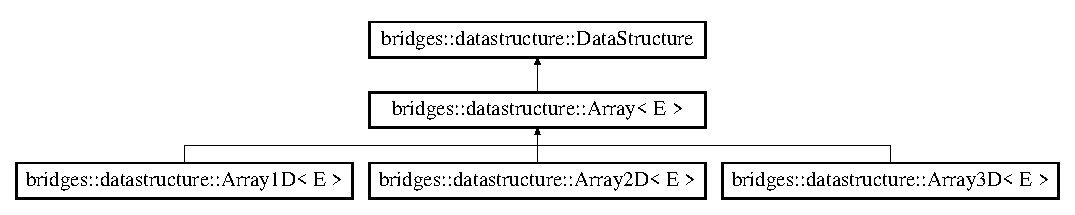
\includegraphics[height=2.445415cm]{classbridges_1_1datastructure_1_1_array}
\end{center}
\end{figure}


\doxysubsection{Detailed Description}
\subsubsection*{template$<$typename E$>$\newline
class bridges\+::datastructure\+::\+Array$<$ E $>$}

The foundation of BRIDGES array types. It is not meant to be used directly by students. 

This class can be used to create 1D, 2D, and 3D arrays of any type.


\begin{DoxyParams}{Parameters}
{\em E} & the application data type\\
\hline
\end{DoxyParams}
\begin{DoxyAuthor}{Author}
Kalpathi Subramanian 
\end{DoxyAuthor}
\begin{DoxyDate}{Date}
1/14/17, 7/12/19 
\end{DoxyDate}
\doxysubsection*{Public Member Functions}
\begin{DoxyCompactItemize}
\item 
virtual const string \mbox{\hyperlink{classbridges_1_1datastructure_1_1_array_a3b6d694fe5d336a0a15951d522852e51}{get\+DStype}} () const override
\item 
virtual const string \mbox{\hyperlink{classbridges_1_1datastructure_1_1_array_a210de6729fa08715c13d2deb0b141010}{get\+Data\+Structure\+Representation}} () const override final
\item 
\mbox{\hyperlink{classbridges_1_1datastructure_1_1_array_abd017f8feb1d892e8559df6533354d3f}{Array}} (const \mbox{\hyperlink{classbridges_1_1datastructure_1_1_array}{Array}} \&)=delete
\item 
\mbox{\hyperlink{classbridges_1_1datastructure_1_1_array}{Array}} \& \mbox{\hyperlink{classbridges_1_1datastructure_1_1_array_a5ca19edaaf0eeba81f73440384eddeb4}{operator=}} (const \mbox{\hyperlink{classbridges_1_1datastructure_1_1_array}{Array}} \&)=delete
\end{DoxyCompactItemize}
\doxysubsection*{Protected Member Functions}
\begin{DoxyCompactItemize}
\item 
\mbox{\hyperlink{classbridges_1_1datastructure_1_1_array_a23cb659c4f39e5e6f3b29a58e97b8e0d}{Array}} ()
\item 
virtual \mbox{\hyperlink{classbridges_1_1datastructure_1_1_array_a5a9f212f560e9673259eece27d8f11cc}{$\sim$\+Array}} ()
\item 
\mbox{\hyperlink{classbridges_1_1datastructure_1_1_array_ad72d4311346c5b9e53ee8eff2a4aadce}{Array}} (int sz)
\begin{DoxyCompactList}\small\item\em builds an array given the size \end{DoxyCompactList}\item 
void \mbox{\hyperlink{classbridges_1_1datastructure_1_1_array_a2bfb10e98b1745a7ca173459626352a9}{set\+Size}} (int nd, int $\ast$dim)
\begin{DoxyCompactList}\small\item\em Set the size of the array. \end{DoxyCompactList}\item 
void \mbox{\hyperlink{classbridges_1_1datastructure_1_1_array_aa2a14939c8e53087e833ebf71822a057}{get\+Dimensions}} (int $\ast$dim)
\begin{DoxyCompactList}\small\item\em Get the dimensions of the array. \end{DoxyCompactList}\item 
int const  $\ast$ \mbox{\hyperlink{classbridges_1_1datastructure_1_1_array_a6d9edc546fa172a47f19de3c2ea93ebf}{get\+Dimensions}} () const
\item 
\mbox{\hyperlink{classbridges_1_1datastructure_1_1_element}{Element}}$<$ E $>$ \& \mbox{\hyperlink{classbridges_1_1datastructure_1_1_array_aaf44dbc671651d6e1383d1c523348f28}{get\+Element}} (int index)
\item 
\mbox{\hyperlink{classbridges_1_1datastructure_1_1_element}{Element}}$<$ E $>$ const  \& \mbox{\hyperlink{classbridges_1_1datastructure_1_1_array_ad2704d36d824ef7356fda5f6d7974ba7}{get\+Element}} (int index) const
\begin{DoxyCompactList}\small\item\em Get the object at index index -\/ 1D array. \end{DoxyCompactList}\item 
void \mbox{\hyperlink{classbridges_1_1datastructure_1_1_array_a120174198dc4de388af154d97951e856}{set\+Element}} (int ind, \mbox{\hyperlink{classbridges_1_1datastructure_1_1_element}{Element}}$<$ E $>$ el)
\begin{DoxyCompactList}\small\item\em Set the \mbox{\hyperlink{classbridges_1_1datastructure_1_1_element}{Element}} at index ind -\/ 1D array. \end{DoxyCompactList}\end{DoxyCompactItemize}
\doxysubsection*{Friends}
\begin{DoxyCompactItemize}
\item 
class \mbox{\hyperlink{classbridges_1_1datastructure_1_1_array_a8c6ff2a8dd3e27346dd25f588a78828a}{Element$<$ E $>$}}
\end{DoxyCompactItemize}


\doxysubsection{Constructor \& Destructor Documentation}
\mbox{\Hypertarget{classbridges_1_1datastructure_1_1_array_a23cb659c4f39e5e6f3b29a58e97b8e0d}\label{classbridges_1_1datastructure_1_1_array_a23cb659c4f39e5e6f3b29a58e97b8e0d}} 
\index{bridges::datastructure::Array$<$ E $>$@{bridges::datastructure::Array$<$ E $>$}!Array@{Array}}
\index{Array@{Array}!bridges::datastructure::Array$<$ E $>$@{bridges::datastructure::Array$<$ E $>$}}
\doxysubsubsection{\texorpdfstring{Array()}{Array()}\hspace{0.1cm}{\footnotesize\ttfamily [1/3]}}
{\footnotesize\ttfamily template$<$typename E $>$ \\
\mbox{\hyperlink{classbridges_1_1datastructure_1_1_array}{bridges\+::datastructure\+::\+Array}}$<$ E $>$\+::\mbox{\hyperlink{classbridges_1_1datastructure_1_1_array}{Array}} (\begin{DoxyParamCaption}{ }\end{DoxyParamCaption})\hspace{0.3cm}{\ttfamily [inline]}, {\ttfamily [protected]}}

\mbox{\Hypertarget{classbridges_1_1datastructure_1_1_array_a5a9f212f560e9673259eece27d8f11cc}\label{classbridges_1_1datastructure_1_1_array_a5a9f212f560e9673259eece27d8f11cc}} 
\index{bridges::datastructure::Array$<$ E $>$@{bridges::datastructure::Array$<$ E $>$}!````~Array@{$\sim$Array}}
\index{````~Array@{$\sim$Array}!bridges::datastructure::Array$<$ E $>$@{bridges::datastructure::Array$<$ E $>$}}
\doxysubsubsection{\texorpdfstring{$\sim$Array()}{~Array()}}
{\footnotesize\ttfamily template$<$typename E $>$ \\
virtual \mbox{\hyperlink{classbridges_1_1datastructure_1_1_array}{bridges\+::datastructure\+::\+Array}}$<$ E $>$\+::$\sim$\mbox{\hyperlink{classbridges_1_1datastructure_1_1_array}{Array}} (\begin{DoxyParamCaption}{ }\end{DoxyParamCaption})\hspace{0.3cm}{\ttfamily [inline]}, {\ttfamily [protected]}, {\ttfamily [virtual]}}

\mbox{\Hypertarget{classbridges_1_1datastructure_1_1_array_ad72d4311346c5b9e53ee8eff2a4aadce}\label{classbridges_1_1datastructure_1_1_array_ad72d4311346c5b9e53ee8eff2a4aadce}} 
\index{bridges::datastructure::Array$<$ E $>$@{bridges::datastructure::Array$<$ E $>$}!Array@{Array}}
\index{Array@{Array}!bridges::datastructure::Array$<$ E $>$@{bridges::datastructure::Array$<$ E $>$}}
\doxysubsubsection{\texorpdfstring{Array()}{Array()}\hspace{0.1cm}{\footnotesize\ttfamily [2/3]}}
{\footnotesize\ttfamily template$<$typename E $>$ \\
\mbox{\hyperlink{classbridges_1_1datastructure_1_1_array}{bridges\+::datastructure\+::\+Array}}$<$ E $>$\+::\mbox{\hyperlink{classbridges_1_1datastructure_1_1_array}{Array}} (\begin{DoxyParamCaption}\item[{int}]{sz }\end{DoxyParamCaption})\hspace{0.3cm}{\ttfamily [inline]}, {\ttfamily [protected]}}



builds an array given the size 


\begin{DoxyParams}{Parameters}
{\em sz} & size of array \\
\hline
\end{DoxyParams}
\mbox{\Hypertarget{classbridges_1_1datastructure_1_1_array_abd017f8feb1d892e8559df6533354d3f}\label{classbridges_1_1datastructure_1_1_array_abd017f8feb1d892e8559df6533354d3f}} 
\index{bridges::datastructure::Array$<$ E $>$@{bridges::datastructure::Array$<$ E $>$}!Array@{Array}}
\index{Array@{Array}!bridges::datastructure::Array$<$ E $>$@{bridges::datastructure::Array$<$ E $>$}}
\doxysubsubsection{\texorpdfstring{Array()}{Array()}\hspace{0.1cm}{\footnotesize\ttfamily [3/3]}}
{\footnotesize\ttfamily template$<$typename E $>$ \\
\mbox{\hyperlink{classbridges_1_1datastructure_1_1_array}{bridges\+::datastructure\+::\+Array}}$<$ E $>$\+::\mbox{\hyperlink{classbridges_1_1datastructure_1_1_array}{Array}} (\begin{DoxyParamCaption}\item[{const \mbox{\hyperlink{classbridges_1_1datastructure_1_1_array}{Array}}$<$ E $>$ \&}]{ }\end{DoxyParamCaption})\hspace{0.3cm}{\ttfamily [delete]}}



\doxysubsection{Member Function Documentation}
\mbox{\Hypertarget{classbridges_1_1datastructure_1_1_array_a210de6729fa08715c13d2deb0b141010}\label{classbridges_1_1datastructure_1_1_array_a210de6729fa08715c13d2deb0b141010}} 
\index{bridges::datastructure::Array$<$ E $>$@{bridges::datastructure::Array$<$ E $>$}!getDataStructureRepresentation@{getDataStructureRepresentation}}
\index{getDataStructureRepresentation@{getDataStructureRepresentation}!bridges::datastructure::Array$<$ E $>$@{bridges::datastructure::Array$<$ E $>$}}
\doxysubsubsection{\texorpdfstring{getDataStructureRepresentation()}{getDataStructureRepresentation()}}
{\footnotesize\ttfamily template$<$typename E $>$ \\
virtual const string \mbox{\hyperlink{classbridges_1_1datastructure_1_1_array}{bridges\+::datastructure\+::\+Array}}$<$ E $>$\+::get\+Data\+Structure\+Representation (\begin{DoxyParamCaption}{ }\end{DoxyParamCaption}) const\hspace{0.3cm}{\ttfamily [inline]}, {\ttfamily [final]}, {\ttfamily [override]}, {\ttfamily [virtual]}}

Ease of use function for the deletion of an entire datastructure. Overrides should call delete on itself and each linked data structure

\begin{DoxyWarning}{Warning}
Only call if all these data structures were all dynamicaly allocated(aka\+: using new) Gets the JSON representation of this \mbox{\hyperlink{classbridges_1_1datastructure_1_1_data_structure}{Data\+Structure}}\textquotesingle{}s nodes and links
\end{DoxyWarning}
\begin{DoxyReturn}{Returns}
The JSON representation of the data structure\+: A pair holding the nodes and links JSON strings respectively 
\end{DoxyReturn}


Implements \mbox{\hyperlink{classbridges_1_1datastructure_1_1_data_structure}{bridges\+::datastructure\+::\+Data\+Structure}}.

\mbox{\Hypertarget{classbridges_1_1datastructure_1_1_array_a6d9edc546fa172a47f19de3c2ea93ebf}\label{classbridges_1_1datastructure_1_1_array_a6d9edc546fa172a47f19de3c2ea93ebf}} 
\index{bridges::datastructure::Array$<$ E $>$@{bridges::datastructure::Array$<$ E $>$}!getDimensions@{getDimensions}}
\index{getDimensions@{getDimensions}!bridges::datastructure::Array$<$ E $>$@{bridges::datastructure::Array$<$ E $>$}}
\doxysubsubsection{\texorpdfstring{getDimensions()}{getDimensions()}\hspace{0.1cm}{\footnotesize\ttfamily [1/2]}}
{\footnotesize\ttfamily template$<$typename E $>$ \\
int const$\ast$ \mbox{\hyperlink{classbridges_1_1datastructure_1_1_array}{bridges\+::datastructure\+::\+Array}}$<$ E $>$\+::get\+Dimensions (\begin{DoxyParamCaption}{ }\end{DoxyParamCaption}) const\hspace{0.3cm}{\ttfamily [inline]}, {\ttfamily [protected]}}

\mbox{\Hypertarget{classbridges_1_1datastructure_1_1_array_aa2a14939c8e53087e833ebf71822a057}\label{classbridges_1_1datastructure_1_1_array_aa2a14939c8e53087e833ebf71822a057}} 
\index{bridges::datastructure::Array$<$ E $>$@{bridges::datastructure::Array$<$ E $>$}!getDimensions@{getDimensions}}
\index{getDimensions@{getDimensions}!bridges::datastructure::Array$<$ E $>$@{bridges::datastructure::Array$<$ E $>$}}
\doxysubsubsection{\texorpdfstring{getDimensions()}{getDimensions()}\hspace{0.1cm}{\footnotesize\ttfamily [2/2]}}
{\footnotesize\ttfamily template$<$typename E $>$ \\
void \mbox{\hyperlink{classbridges_1_1datastructure_1_1_array}{bridges\+::datastructure\+::\+Array}}$<$ E $>$\+::get\+Dimensions (\begin{DoxyParamCaption}\item[{int $\ast$}]{dim }\end{DoxyParamCaption})\hspace{0.3cm}{\ttfamily [inline]}, {\ttfamily [protected]}}



Get the dimensions of the array. 


\begin{DoxyParams}[1]{Parameters}
\mbox{\texttt{ out}}  & {\em dim} & an array to return the dimensions \\
\hline
\end{DoxyParams}
\mbox{\Hypertarget{classbridges_1_1datastructure_1_1_array_a3b6d694fe5d336a0a15951d522852e51}\label{classbridges_1_1datastructure_1_1_array_a3b6d694fe5d336a0a15951d522852e51}} 
\index{bridges::datastructure::Array$<$ E $>$@{bridges::datastructure::Array$<$ E $>$}!getDStype@{getDStype}}
\index{getDStype@{getDStype}!bridges::datastructure::Array$<$ E $>$@{bridges::datastructure::Array$<$ E $>$}}
\doxysubsubsection{\texorpdfstring{getDStype()}{getDStype()}}
{\footnotesize\ttfamily template$<$typename E $>$ \\
virtual const string \mbox{\hyperlink{classbridges_1_1datastructure_1_1_array}{bridges\+::datastructure\+::\+Array}}$<$ E $>$\+::get\+DStype (\begin{DoxyParamCaption}{ }\end{DoxyParamCaption}) const\hspace{0.3cm}{\ttfamily [inline]}, {\ttfamily [override]}, {\ttfamily [virtual]}}

Get the data structure type \begin{DoxyReturn}{Returns}
data structure name 
\end{DoxyReturn}


Implements \mbox{\hyperlink{classbridges_1_1datastructure_1_1_data_structure_a4ff66cb34409f11fe9fc647f6d8a22ce}{bridges\+::datastructure\+::\+Data\+Structure}}.

\mbox{\Hypertarget{classbridges_1_1datastructure_1_1_array_aaf44dbc671651d6e1383d1c523348f28}\label{classbridges_1_1datastructure_1_1_array_aaf44dbc671651d6e1383d1c523348f28}} 
\index{bridges::datastructure::Array$<$ E $>$@{bridges::datastructure::Array$<$ E $>$}!getElement@{getElement}}
\index{getElement@{getElement}!bridges::datastructure::Array$<$ E $>$@{bridges::datastructure::Array$<$ E $>$}}
\doxysubsubsection{\texorpdfstring{getElement()}{getElement()}\hspace{0.1cm}{\footnotesize\ttfamily [1/2]}}
{\footnotesize\ttfamily template$<$typename E $>$ \\
\mbox{\hyperlink{classbridges_1_1datastructure_1_1_element}{Element}}$<$E$>$\& \mbox{\hyperlink{classbridges_1_1datastructure_1_1_array}{bridges\+::datastructure\+::\+Array}}$<$ E $>$\+::get\+Element (\begin{DoxyParamCaption}\item[{int}]{index }\end{DoxyParamCaption})\hspace{0.3cm}{\ttfamily [inline]}, {\ttfamily [protected]}}

Get the object at index index -\/ 1D array


\begin{DoxyParams}{Parameters}
{\em index} & index into the array\\
\hline
\end{DoxyParams}
\begin{DoxyReturn}{Returns}
the \mbox{\hyperlink{classbridges_1_1datastructure_1_1_element}{Element}} at \textquotesingle{}index\textquotesingle{} 
\end{DoxyReturn}
\mbox{\Hypertarget{classbridges_1_1datastructure_1_1_array_ad2704d36d824ef7356fda5f6d7974ba7}\label{classbridges_1_1datastructure_1_1_array_ad2704d36d824ef7356fda5f6d7974ba7}} 
\index{bridges::datastructure::Array$<$ E $>$@{bridges::datastructure::Array$<$ E $>$}!getElement@{getElement}}
\index{getElement@{getElement}!bridges::datastructure::Array$<$ E $>$@{bridges::datastructure::Array$<$ E $>$}}
\doxysubsubsection{\texorpdfstring{getElement()}{getElement()}\hspace{0.1cm}{\footnotesize\ttfamily [2/2]}}
{\footnotesize\ttfamily template$<$typename E $>$ \\
\mbox{\hyperlink{classbridges_1_1datastructure_1_1_element}{Element}}$<$E$>$ const\& \mbox{\hyperlink{classbridges_1_1datastructure_1_1_array}{bridges\+::datastructure\+::\+Array}}$<$ E $>$\+::get\+Element (\begin{DoxyParamCaption}\item[{int}]{index }\end{DoxyParamCaption}) const\hspace{0.3cm}{\ttfamily [inline]}, {\ttfamily [protected]}}



Get the object at index index -\/ 1D array. 


\begin{DoxyParams}{Parameters}
{\em index} & -\/ index into the array\\
\hline
\end{DoxyParams}
\begin{DoxyReturn}{Returns}
the \mbox{\hyperlink{classbridges_1_1datastructure_1_1_element}{Element}} at \textquotesingle{}index\textquotesingle{} 
\end{DoxyReturn}
\mbox{\Hypertarget{classbridges_1_1datastructure_1_1_array_a5ca19edaaf0eeba81f73440384eddeb4}\label{classbridges_1_1datastructure_1_1_array_a5ca19edaaf0eeba81f73440384eddeb4}} 
\index{bridges::datastructure::Array$<$ E $>$@{bridges::datastructure::Array$<$ E $>$}!operator=@{operator=}}
\index{operator=@{operator=}!bridges::datastructure::Array$<$ E $>$@{bridges::datastructure::Array$<$ E $>$}}
\doxysubsubsection{\texorpdfstring{operator=()}{operator=()}}
{\footnotesize\ttfamily template$<$typename E $>$ \\
\mbox{\hyperlink{classbridges_1_1datastructure_1_1_array}{Array}}\& \mbox{\hyperlink{classbridges_1_1datastructure_1_1_array}{bridges\+::datastructure\+::\+Array}}$<$ E $>$\+::operator= (\begin{DoxyParamCaption}\item[{const \mbox{\hyperlink{classbridges_1_1datastructure_1_1_array}{Array}}$<$ E $>$ \&}]{ }\end{DoxyParamCaption})\hspace{0.3cm}{\ttfamily [delete]}}

\mbox{\Hypertarget{classbridges_1_1datastructure_1_1_array_a120174198dc4de388af154d97951e856}\label{classbridges_1_1datastructure_1_1_array_a120174198dc4de388af154d97951e856}} 
\index{bridges::datastructure::Array$<$ E $>$@{bridges::datastructure::Array$<$ E $>$}!setElement@{setElement}}
\index{setElement@{setElement}!bridges::datastructure::Array$<$ E $>$@{bridges::datastructure::Array$<$ E $>$}}
\doxysubsubsection{\texorpdfstring{setElement()}{setElement()}}
{\footnotesize\ttfamily template$<$typename E $>$ \\
void \mbox{\hyperlink{classbridges_1_1datastructure_1_1_array}{bridges\+::datastructure\+::\+Array}}$<$ E $>$\+::set\+Element (\begin{DoxyParamCaption}\item[{int}]{ind,  }\item[{\mbox{\hyperlink{classbridges_1_1datastructure_1_1_element}{Element}}$<$ E $>$}]{el }\end{DoxyParamCaption})\hspace{0.3cm}{\ttfamily [inline]}, {\ttfamily [protected]}}



Set the \mbox{\hyperlink{classbridges_1_1datastructure_1_1_element}{Element}} at index ind -\/ 1D array. 


\begin{DoxyParams}{Parameters}
{\em ind} & index into the array \\
\hline
{\em el} & \mbox{\hyperlink{classbridges_1_1datastructure_1_1_element}{Element}} object \\
\hline
\end{DoxyParams}
\mbox{\Hypertarget{classbridges_1_1datastructure_1_1_array_a2bfb10e98b1745a7ca173459626352a9}\label{classbridges_1_1datastructure_1_1_array_a2bfb10e98b1745a7ca173459626352a9}} 
\index{bridges::datastructure::Array$<$ E $>$@{bridges::datastructure::Array$<$ E $>$}!setSize@{setSize}}
\index{setSize@{setSize}!bridges::datastructure::Array$<$ E $>$@{bridges::datastructure::Array$<$ E $>$}}
\doxysubsubsection{\texorpdfstring{setSize()}{setSize()}}
{\footnotesize\ttfamily template$<$typename E $>$ \\
void \mbox{\hyperlink{classbridges_1_1datastructure_1_1_array}{bridges\+::datastructure\+::\+Array}}$<$ E $>$\+::set\+Size (\begin{DoxyParamCaption}\item[{int}]{nd,  }\item[{int $\ast$}]{dim }\end{DoxyParamCaption})\hspace{0.3cm}{\ttfamily [inline]}, {\ttfamily [protected]}}



Set the size of the array. 


\begin{DoxyParams}[1]{Parameters}
\mbox{\texttt{ in}}  & {\em nd} & number of dimension \\
\hline
\mbox{\texttt{ in}}  & {\em dim} & the size of the dimensions \\
\hline
\end{DoxyParams}


\doxysubsection{Friends And Related Function Documentation}
\mbox{\Hypertarget{classbridges_1_1datastructure_1_1_array_a8c6ff2a8dd3e27346dd25f588a78828a}\label{classbridges_1_1datastructure_1_1_array_a8c6ff2a8dd3e27346dd25f588a78828a}} 
\index{bridges::datastructure::Array$<$ E $>$@{bridges::datastructure::Array$<$ E $>$}!Element$<$ E $>$@{Element$<$ E $>$}}
\index{Element$<$ E $>$@{Element$<$ E $>$}!bridges::datastructure::Array$<$ E $>$@{bridges::datastructure::Array$<$ E $>$}}
\doxysubsubsection{\texorpdfstring{Element$<$ E $>$}{Element< E >}}
{\footnotesize\ttfamily template$<$typename E $>$ \\
friend class \mbox{\hyperlink{classbridges_1_1datastructure_1_1_element}{Element}}$<$ E $>$\hspace{0.3cm}{\ttfamily [friend]}}



The documentation for this class was generated from the following file\+:\begin{DoxyCompactItemize}
\item 
/home/erik/work/bridges/bridges-\/cxx/src/\mbox{\hyperlink{_array_8h}{Array.\+h}}\end{DoxyCompactItemize}

\hypertarget{classbridges_1_1datastructure_1_1_array1_d}{}\section{bridges\+:\+:datastructure\+:\+:Array1D$<$ E $>$ Class Template Reference}
\label{classbridges_1_1datastructure_1_1_array1_d}\index{bridges\+::datastructure\+::\+Array1\+D$<$ E $>$@{bridges\+::datastructure\+::\+Array1\+D$<$ E $>$}}


{\ttfamily \#include $<$Array1\+D.\+h$>$}

Inheritance diagram for bridges\+:\+:datastructure\+:\+:Array1D$<$ E $>$\+:\begin{figure}[H]
\begin{center}
\leavevmode
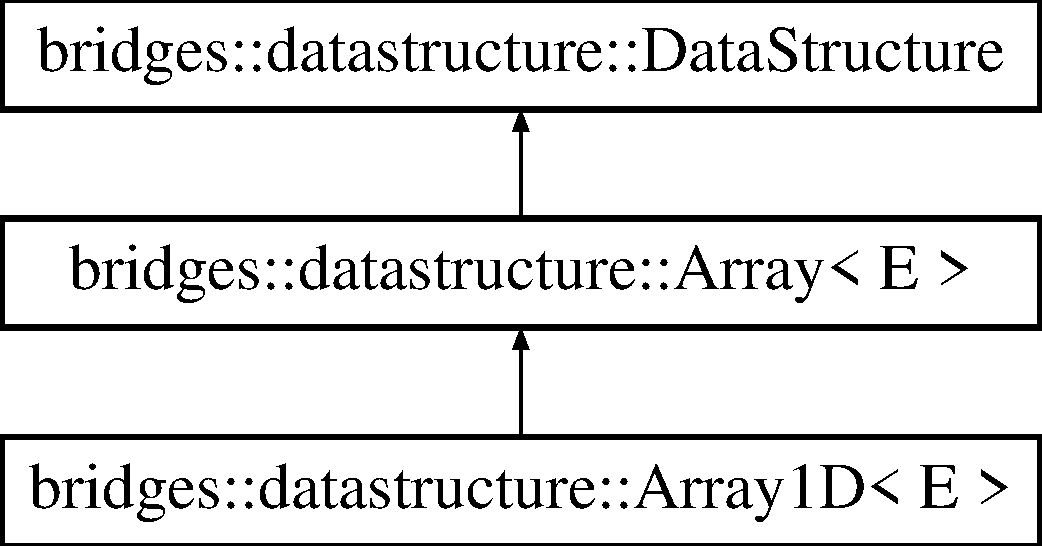
\includegraphics[height=3.000000cm]{classbridges_1_1datastructure_1_1_array1_d}
\end{center}
\end{figure}


\subsection{Detailed Description}
\subsubsection*{template$<$typename E$>$\newline
class bridges\+::datastructure\+::\+Array1\+D$<$ E $>$}

A B\+R\+I\+D\+G\+ES 1D array type. 

This class can be used to create 1D arrays of any type.

The class stores an array of E where each entry can be styled.

The access to the values stored are done directly using bracket operators such as


\begin{DoxyCode}
Array1D<std::string> arr(19);
arr [12] = \textcolor{stringliteral}{"hello!"};
\end{DoxyCode}


Entries in the array can be styled by showing a label and changing the color of an entry. This is achieved by styling the underlying element to a particular entry of the array such as\+:


\begin{DoxyCode}
Array1D<std::string> arr(19);
arr.getElement(12).setColor(\textcolor{stringliteral}{"yellow"});
arr.getElement(12).setLabel(\textcolor{stringliteral}{"Hi there"});
\end{DoxyCode}


The array support range for loop so you can get to all elements in the array using \+:


\begin{DoxyCode}
Array1D<std::string> arr(19);
\textcolor{keywordflow}{for} (\textcolor{keyword}{auto} mystring : arr) \{
  std::cout<<mystring<<\textcolor{stringliteral}{"\(\backslash\)n"};
\}
\end{DoxyCode}



\begin{DoxyParams}{Parameters}
{\em E} & the application data type \\
\hline
\end{DoxyParams}
\begin{DoxyAuthor}{Author}
Kalpathi Subramanian, Erik Saule 
\end{DoxyAuthor}
\begin{DoxyDate}{Date}
7/16/19 
\end{DoxyDate}
\subsection*{Classes}
\begin{DoxyCompactItemize}
\item 
class \hyperlink{classbridges_1_1datastructure_1_1_array1_d_1_1const__iterator}{const\+\_\+iterator}
\begin{DoxyCompactList}\small\item\em enabling iterator loops in const contexts \end{DoxyCompactList}\item 
class \hyperlink{classbridges_1_1datastructure_1_1_array1_d_1_1iterator}{iterator}
\begin{DoxyCompactList}\small\item\em enabling range for loops \end{DoxyCompactList}\end{DoxyCompactItemize}
\subsection*{Public Member Functions}
\begin{DoxyCompactItemize}
\item 
virtual \hyperlink{classbridges_1_1datastructure_1_1_array1_d_a690a7802e32842acfda2688459bb2caa}{$\sim$\+Array1D} ()
\item 
\hyperlink{classbridges_1_1datastructure_1_1_array1_d_a04e070ed24a1c6e9d200add01ec91c95}{Array1D} (int sz)
\begin{DoxyCompactList}\small\item\em builds an array given size \end{DoxyCompactList}\item 
E \& \hyperlink{classbridges_1_1datastructure_1_1_array1_d_ac0e28b33231ba865d00dbaf1ad4d1b5b}{operator\mbox{[}$\,$\mbox{]}} (int indx)
\begin{DoxyCompactList}\small\item\em access \hyperlink{classbridges_1_1datastructure_1_1_array}{Array}\mbox{[}indx\mbox{]} \end{DoxyCompactList}\item 
E const  \& \hyperlink{classbridges_1_1datastructure_1_1_array1_d_a3eee632c4ba3bce5694da00f07e1ac65}{operator\mbox{[}$\,$\mbox{]}} (int indx) const
\begin{DoxyCompactList}\small\item\em access \hyperlink{classbridges_1_1datastructure_1_1_array}{Array}\mbox{[}indx\mbox{]} \end{DoxyCompactList}\item 
\hyperlink{classbridges_1_1datastructure_1_1_element}{Element}$<$ E $>$ \& \hyperlink{classbridges_1_1datastructure_1_1_array1_d_a48fbe4ee71c52303033effcd4e1369c0}{get\+Element} (int indx)
\begin{DoxyCompactList}\small\item\em access the element that stores \hyperlink{classbridges_1_1datastructure_1_1_array}{Array}\mbox{[}indx\mbox{]} \end{DoxyCompactList}\item 
\hyperlink{classbridges_1_1datastructure_1_1_element}{Element}$<$ E $>$ const  \& \hyperlink{classbridges_1_1datastructure_1_1_array1_d_a92398a260b9d2a09d6f1f536a36a0988}{get\+Element} (int indx) const
\begin{DoxyCompactList}\small\item\em access the element that stores \hyperlink{classbridges_1_1datastructure_1_1_array}{Array}\mbox{[}indx\mbox{]} \end{DoxyCompactList}\item 
void \hyperlink{classbridges_1_1datastructure_1_1_array1_d_a1494c33b1f37bc4c9bc983f1f181488f}{set\+Element} (int indx, const \hyperlink{classbridges_1_1datastructure_1_1_element}{Element}$<$ E $>$ \&e)
\begin{DoxyCompactList}\small\item\em change the element that stores \hyperlink{classbridges_1_1datastructure_1_1_array}{Array}\mbox{[}indx\mbox{]} \end{DoxyCompactList}\item 
\hyperlink{classbridges_1_1datastructure_1_1_array1_d_1_1iterator}{iterator} \hyperlink{classbridges_1_1datastructure_1_1_array1_d_ad93131c3f7f2e446bedc02d36ac7ddc5}{begin} ()
\begin{DoxyCompactList}\small\item\em enables range for loops \end{DoxyCompactList}\item 
\hyperlink{classbridges_1_1datastructure_1_1_array1_d_1_1iterator}{iterator} \hyperlink{classbridges_1_1datastructure_1_1_array1_d_a238e21eb9afcd0f32e3612b36b7d1a2a}{end} ()
\begin{DoxyCompactList}\small\item\em enables range for loops \end{DoxyCompactList}\item 
\hyperlink{classbridges_1_1datastructure_1_1_array1_d_1_1const__iterator}{const\+\_\+iterator} \hyperlink{classbridges_1_1datastructure_1_1_array1_d_a61e7a77165129de2016633ce24284417}{begin} () const
\begin{DoxyCompactList}\small\item\em enables range for loops \end{DoxyCompactList}\item 
\hyperlink{classbridges_1_1datastructure_1_1_array1_d_1_1const__iterator}{const\+\_\+iterator} \hyperlink{classbridges_1_1datastructure_1_1_array1_d_afa8c2d7cb3db9a506baa18d383aabdb5}{end} () const
\begin{DoxyCompactList}\small\item\em enables range for loops \end{DoxyCompactList}\end{DoxyCompactItemize}
\subsection*{Additional Inherited Members}


\subsection{Constructor \& Destructor Documentation}
\mbox{\Hypertarget{classbridges_1_1datastructure_1_1_array1_d_a690a7802e32842acfda2688459bb2caa}\label{classbridges_1_1datastructure_1_1_array1_d_a690a7802e32842acfda2688459bb2caa}} 
\index{bridges\+::datastructure\+::\+Array1D@{bridges\+::datastructure\+::\+Array1D}!````~Array1D@{$\sim$\+Array1D}}
\index{````~Array1D@{$\sim$\+Array1D}!bridges\+::datastructure\+::\+Array1D@{bridges\+::datastructure\+::\+Array1D}}
\subsubsection{\texorpdfstring{$\sim$\+Array1\+D()}{~Array1D()}}
{\footnotesize\ttfamily template$<$typename E$>$ \\
virtual \hyperlink{classbridges_1_1datastructure_1_1_array1_d}{bridges\+::datastructure\+::\+Array1D}$<$ E $>$\+::$\sim$\hyperlink{classbridges_1_1datastructure_1_1_array1_d}{Array1D} (\begin{DoxyParamCaption}{ }\end{DoxyParamCaption})\hspace{0.3cm}{\ttfamily [inline]}, {\ttfamily [virtual]}}

\mbox{\Hypertarget{classbridges_1_1datastructure_1_1_array1_d_a04e070ed24a1c6e9d200add01ec91c95}\label{classbridges_1_1datastructure_1_1_array1_d_a04e070ed24a1c6e9d200add01ec91c95}} 
\index{bridges\+::datastructure\+::\+Array1D@{bridges\+::datastructure\+::\+Array1D}!Array1D@{Array1D}}
\index{Array1D@{Array1D}!bridges\+::datastructure\+::\+Array1D@{bridges\+::datastructure\+::\+Array1D}}
\subsubsection{\texorpdfstring{Array1\+D()}{Array1D()}}
{\footnotesize\ttfamily template$<$typename E$>$ \\
\hyperlink{classbridges_1_1datastructure_1_1_array1_d}{bridges\+::datastructure\+::\+Array1D}$<$ E $>$\+::\hyperlink{classbridges_1_1datastructure_1_1_array1_d}{Array1D} (\begin{DoxyParamCaption}\item[{int}]{sz }\end{DoxyParamCaption})\hspace{0.3cm}{\ttfamily [inline]}}



builds an array given size 


\begin{DoxyParams}{Parameters}
{\em sz} & size of the array \\
\hline
\end{DoxyParams}


\subsection{Member Function Documentation}
\mbox{\Hypertarget{classbridges_1_1datastructure_1_1_array1_d_ad93131c3f7f2e446bedc02d36ac7ddc5}\label{classbridges_1_1datastructure_1_1_array1_d_ad93131c3f7f2e446bedc02d36ac7ddc5}} 
\index{bridges\+::datastructure\+::\+Array1D@{bridges\+::datastructure\+::\+Array1D}!begin@{begin}}
\index{begin@{begin}!bridges\+::datastructure\+::\+Array1D@{bridges\+::datastructure\+::\+Array1D}}
\subsubsection{\texorpdfstring{begin()}{begin()}\hspace{0.1cm}{\footnotesize\ttfamily [1/2]}}
{\footnotesize\ttfamily template$<$typename E$>$ \\
\hyperlink{classbridges_1_1datastructure_1_1_array1_d_1_1iterator}{iterator} \hyperlink{classbridges_1_1datastructure_1_1_array1_d}{bridges\+::datastructure\+::\+Array1D}$<$ E $>$\+::begin (\begin{DoxyParamCaption}{ }\end{DoxyParamCaption})\hspace{0.3cm}{\ttfamily [inline]}}



enables range for loops 

\mbox{\Hypertarget{classbridges_1_1datastructure_1_1_array1_d_a61e7a77165129de2016633ce24284417}\label{classbridges_1_1datastructure_1_1_array1_d_a61e7a77165129de2016633ce24284417}} 
\index{bridges\+::datastructure\+::\+Array1D@{bridges\+::datastructure\+::\+Array1D}!begin@{begin}}
\index{begin@{begin}!bridges\+::datastructure\+::\+Array1D@{bridges\+::datastructure\+::\+Array1D}}
\subsubsection{\texorpdfstring{begin()}{begin()}\hspace{0.1cm}{\footnotesize\ttfamily [2/2]}}
{\footnotesize\ttfamily template$<$typename E$>$ \\
\hyperlink{classbridges_1_1datastructure_1_1_array1_d_1_1const__iterator}{const\+\_\+iterator} \hyperlink{classbridges_1_1datastructure_1_1_array1_d}{bridges\+::datastructure\+::\+Array1D}$<$ E $>$\+::begin (\begin{DoxyParamCaption}{ }\end{DoxyParamCaption}) const\hspace{0.3cm}{\ttfamily [inline]}}



enables range for loops 

\mbox{\Hypertarget{classbridges_1_1datastructure_1_1_array1_d_a238e21eb9afcd0f32e3612b36b7d1a2a}\label{classbridges_1_1datastructure_1_1_array1_d_a238e21eb9afcd0f32e3612b36b7d1a2a}} 
\index{bridges\+::datastructure\+::\+Array1D@{bridges\+::datastructure\+::\+Array1D}!end@{end}}
\index{end@{end}!bridges\+::datastructure\+::\+Array1D@{bridges\+::datastructure\+::\+Array1D}}
\subsubsection{\texorpdfstring{end()}{end()}\hspace{0.1cm}{\footnotesize\ttfamily [1/2]}}
{\footnotesize\ttfamily template$<$typename E$>$ \\
\hyperlink{classbridges_1_1datastructure_1_1_array1_d_1_1iterator}{iterator} \hyperlink{classbridges_1_1datastructure_1_1_array1_d}{bridges\+::datastructure\+::\+Array1D}$<$ E $>$\+::end (\begin{DoxyParamCaption}{ }\end{DoxyParamCaption})\hspace{0.3cm}{\ttfamily [inline]}}



enables range for loops 

\mbox{\Hypertarget{classbridges_1_1datastructure_1_1_array1_d_afa8c2d7cb3db9a506baa18d383aabdb5}\label{classbridges_1_1datastructure_1_1_array1_d_afa8c2d7cb3db9a506baa18d383aabdb5}} 
\index{bridges\+::datastructure\+::\+Array1D@{bridges\+::datastructure\+::\+Array1D}!end@{end}}
\index{end@{end}!bridges\+::datastructure\+::\+Array1D@{bridges\+::datastructure\+::\+Array1D}}
\subsubsection{\texorpdfstring{end()}{end()}\hspace{0.1cm}{\footnotesize\ttfamily [2/2]}}
{\footnotesize\ttfamily template$<$typename E$>$ \\
\hyperlink{classbridges_1_1datastructure_1_1_array1_d_1_1const__iterator}{const\+\_\+iterator} \hyperlink{classbridges_1_1datastructure_1_1_array1_d}{bridges\+::datastructure\+::\+Array1D}$<$ E $>$\+::end (\begin{DoxyParamCaption}{ }\end{DoxyParamCaption}) const\hspace{0.3cm}{\ttfamily [inline]}}



enables range for loops 

\mbox{\Hypertarget{classbridges_1_1datastructure_1_1_array1_d_a48fbe4ee71c52303033effcd4e1369c0}\label{classbridges_1_1datastructure_1_1_array1_d_a48fbe4ee71c52303033effcd4e1369c0}} 
\index{bridges\+::datastructure\+::\+Array1D@{bridges\+::datastructure\+::\+Array1D}!get\+Element@{get\+Element}}
\index{get\+Element@{get\+Element}!bridges\+::datastructure\+::\+Array1D@{bridges\+::datastructure\+::\+Array1D}}
\subsubsection{\texorpdfstring{get\+Element()}{getElement()}\hspace{0.1cm}{\footnotesize\ttfamily [1/2]}}
{\footnotesize\ttfamily template$<$typename E$>$ \\
\hyperlink{classbridges_1_1datastructure_1_1_element}{Element}$<$E$>$\& \hyperlink{classbridges_1_1datastructure_1_1_array1_d}{bridges\+::datastructure\+::\+Array1D}$<$ E $>$\+::get\+Element (\begin{DoxyParamCaption}\item[{int}]{indx }\end{DoxyParamCaption})\hspace{0.3cm}{\ttfamily [inline]}}



access the element that stores \hyperlink{classbridges_1_1datastructure_1_1_array}{Array}\mbox{[}indx\mbox{]} 


\begin{DoxyParams}{Parameters}
{\em indx} & index of the Element$<$\+E$>$ to access \\
\hline
\end{DoxyParams}
\mbox{\Hypertarget{classbridges_1_1datastructure_1_1_array1_d_a92398a260b9d2a09d6f1f536a36a0988}\label{classbridges_1_1datastructure_1_1_array1_d_a92398a260b9d2a09d6f1f536a36a0988}} 
\index{bridges\+::datastructure\+::\+Array1D@{bridges\+::datastructure\+::\+Array1D}!get\+Element@{get\+Element}}
\index{get\+Element@{get\+Element}!bridges\+::datastructure\+::\+Array1D@{bridges\+::datastructure\+::\+Array1D}}
\subsubsection{\texorpdfstring{get\+Element()}{getElement()}\hspace{0.1cm}{\footnotesize\ttfamily [2/2]}}
{\footnotesize\ttfamily template$<$typename E$>$ \\
\hyperlink{classbridges_1_1datastructure_1_1_element}{Element}$<$E$>$ const\& \hyperlink{classbridges_1_1datastructure_1_1_array1_d}{bridges\+::datastructure\+::\+Array1D}$<$ E $>$\+::get\+Element (\begin{DoxyParamCaption}\item[{int}]{indx }\end{DoxyParamCaption}) const\hspace{0.3cm}{\ttfamily [inline]}}



access the element that stores \hyperlink{classbridges_1_1datastructure_1_1_array}{Array}\mbox{[}indx\mbox{]} 


\begin{DoxyParams}{Parameters}
{\em indx} & index of the Element$<$\+E$>$ to access \\
\hline
\end{DoxyParams}
\mbox{\Hypertarget{classbridges_1_1datastructure_1_1_array1_d_ac0e28b33231ba865d00dbaf1ad4d1b5b}\label{classbridges_1_1datastructure_1_1_array1_d_ac0e28b33231ba865d00dbaf1ad4d1b5b}} 
\index{bridges\+::datastructure\+::\+Array1D@{bridges\+::datastructure\+::\+Array1D}!operator\mbox{[}\mbox{]}@{operator[]}}
\index{operator\mbox{[}\mbox{]}@{operator[]}!bridges\+::datastructure\+::\+Array1D@{bridges\+::datastructure\+::\+Array1D}}
\subsubsection{\texorpdfstring{operator[]()}{operator[]()}\hspace{0.1cm}{\footnotesize\ttfamily [1/2]}}
{\footnotesize\ttfamily template$<$typename E$>$ \\
E\& \hyperlink{classbridges_1_1datastructure_1_1_array1_d}{bridges\+::datastructure\+::\+Array1D}$<$ E $>$\+::operator\mbox{[}$\,$\mbox{]} (\begin{DoxyParamCaption}\item[{int}]{indx }\end{DoxyParamCaption})\hspace{0.3cm}{\ttfamily [inline]}}



access \hyperlink{classbridges_1_1datastructure_1_1_array}{Array}\mbox{[}indx\mbox{]} 

\mbox{\Hypertarget{classbridges_1_1datastructure_1_1_array1_d_a3eee632c4ba3bce5694da00f07e1ac65}\label{classbridges_1_1datastructure_1_1_array1_d_a3eee632c4ba3bce5694da00f07e1ac65}} 
\index{bridges\+::datastructure\+::\+Array1D@{bridges\+::datastructure\+::\+Array1D}!operator\mbox{[}\mbox{]}@{operator[]}}
\index{operator\mbox{[}\mbox{]}@{operator[]}!bridges\+::datastructure\+::\+Array1D@{bridges\+::datastructure\+::\+Array1D}}
\subsubsection{\texorpdfstring{operator[]()}{operator[]()}\hspace{0.1cm}{\footnotesize\ttfamily [2/2]}}
{\footnotesize\ttfamily template$<$typename E$>$ \\
E const\& \hyperlink{classbridges_1_1datastructure_1_1_array1_d}{bridges\+::datastructure\+::\+Array1D}$<$ E $>$\+::operator\mbox{[}$\,$\mbox{]} (\begin{DoxyParamCaption}\item[{int}]{indx }\end{DoxyParamCaption}) const\hspace{0.3cm}{\ttfamily [inline]}}



access \hyperlink{classbridges_1_1datastructure_1_1_array}{Array}\mbox{[}indx\mbox{]} 

\mbox{\Hypertarget{classbridges_1_1datastructure_1_1_array1_d_a1494c33b1f37bc4c9bc983f1f181488f}\label{classbridges_1_1datastructure_1_1_array1_d_a1494c33b1f37bc4c9bc983f1f181488f}} 
\index{bridges\+::datastructure\+::\+Array1D@{bridges\+::datastructure\+::\+Array1D}!set\+Element@{set\+Element}}
\index{set\+Element@{set\+Element}!bridges\+::datastructure\+::\+Array1D@{bridges\+::datastructure\+::\+Array1D}}
\subsubsection{\texorpdfstring{set\+Element()}{setElement()}}
{\footnotesize\ttfamily template$<$typename E$>$ \\
void \hyperlink{classbridges_1_1datastructure_1_1_array1_d}{bridges\+::datastructure\+::\+Array1D}$<$ E $>$\+::set\+Element (\begin{DoxyParamCaption}\item[{int}]{indx,  }\item[{const \hyperlink{classbridges_1_1datastructure_1_1_element}{Element}$<$ E $>$ \&}]{e }\end{DoxyParamCaption})\hspace{0.3cm}{\ttfamily [inline]}}



change the element that stores \hyperlink{classbridges_1_1datastructure_1_1_array}{Array}\mbox{[}indx\mbox{]} 


\begin{DoxyParams}{Parameters}
{\em indx} & index of the Element$<$\+E$>$ to change \\
\hline
{\em e} & element to change it to \\
\hline
\end{DoxyParams}


The documentation for this class was generated from the following file\+:\begin{DoxyCompactItemize}
\item 
/home/erik/work/bridges/bridges-\/cxx/src/\hyperlink{_array1_d_8h}{Array1\+D.\+h}\end{DoxyCompactItemize}

\hypertarget{classbridges_1_1datastructure_1_1_array2_d}{}\section{bridges\+:\+:datastructure\+:\+:Array2D$<$ E $>$ Class Template Reference}
\label{classbridges_1_1datastructure_1_1_array2_d}\index{bridges\+::datastructure\+::\+Array2\+D$<$ E $>$@{bridges\+::datastructure\+::\+Array2\+D$<$ E $>$}}


{\ttfamily \#include $<$Array2\+D.\+h$>$}

Inheritance diagram for bridges\+:\+:datastructure\+:\+:Array2D$<$ E $>$\+:\begin{figure}[H]
\begin{center}
\leavevmode
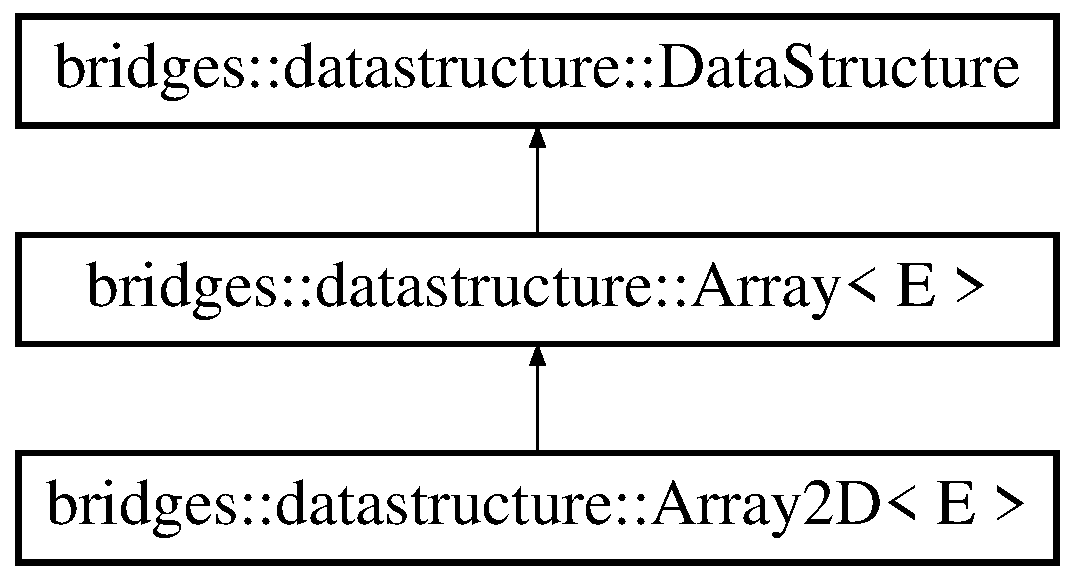
\includegraphics[height=3.000000cm]{classbridges_1_1datastructure_1_1_array2_d}
\end{center}
\end{figure}


\subsection{Detailed Description}
\subsubsection*{template$<$typename E$>$\newline
class bridges\+::datastructure\+::\+Array2\+D$<$ E $>$}

A B\+R\+I\+D\+G\+ES array type. 

This class can be used to create 2D arrays of any type.

The access to the values stored are done directly using bracket operators such as


\begin{DoxyCode}
Array2D<std::string> arr(19, 30);
arr [12][25] = \textcolor{stringliteral}{"hello!"};
\end{DoxyCode}


Entries in the array can be styled by showing a label and changing the color of an entry. This is achieved by styling the underlying element to a particular entry of the array such as\+:


\begin{DoxyCode}
Array2D<std::string> arr(19, 30);
arr.getElement(12, 25).setColor(\textcolor{stringliteral}{"yellow"});
arr.getElement(12, 25).setLabel(\textcolor{stringliteral}{"Hi there"});
\end{DoxyCode}



\begin{DoxyParams}{Parameters}
{\em E} & the application data type\\
\hline
\end{DoxyParams}
\begin{DoxyAuthor}{Author}
Kalpathi Subramanian, Erik Saule 
\end{DoxyAuthor}
\begin{DoxyDate}{Date}
7/16/19 
\end{DoxyDate}
\subsection*{Classes}
\begin{DoxyCompactItemize}
\item 
struct \hyperlink{structbridges_1_1datastructure_1_1_array2_d_1_1_bracket__helper}{Bracket\+\_\+helper}
\begin{DoxyCompactList}\small\item\em helper class to make \mbox{[}\mbox{]}\mbox{[}\mbox{]} operators work on array 2d. You should never use it directly \end{DoxyCompactList}\item 
struct \hyperlink{structbridges_1_1datastructure_1_1_array2_d_1_1_bracket__helper__const}{Bracket\+\_\+helper\+\_\+const}
\begin{DoxyCompactList}\small\item\em helper class to make \mbox{[}\mbox{]}\mbox{[}\mbox{]} operators work on array 2d. You should never use it directly \end{DoxyCompactList}\end{DoxyCompactItemize}
\subsection*{Public Member Functions}
\begin{DoxyCompactItemize}
\item 
virtual \hyperlink{classbridges_1_1datastructure_1_1_array2_d_a6ec24f33b8420735ac7545956afc6dab}{$\sim$\+Array2D} ()
\item 
\hyperlink{classbridges_1_1datastructure_1_1_array2_d_ad65bbb54e829788fee9563a67ffa309c}{Array2D} (int rows, int cols)
\begin{DoxyCompactList}\small\item\em builds an array of given dimensions \end{DoxyCompactList}\item 
int \hyperlink{classbridges_1_1datastructure_1_1_array2_d_afb18017e8a49c0579a90cf22b6dc4c9e}{get\+Num\+Rows} ()
\item 
int \hyperlink{classbridges_1_1datastructure_1_1_array2_d_a0a33557d828d9617871c62a7522817ed}{get\+Num\+Columns} ()
\begin{DoxyCompactList}\small\item\em Gets the number of columns of the 2D array. \end{DoxyCompactList}\item 
\hyperlink{classbridges_1_1datastructure_1_1_element}{Element}$<$ E $>$ \& \hyperlink{classbridges_1_1datastructure_1_1_array2_d_afaa0bcbf06170929d92659314ff2b38d}{get\+Element} (int row, int col)
\item 
void \hyperlink{classbridges_1_1datastructure_1_1_array2_d_a2bd2ef3a200e4a07a4d45534bd31387d}{set\+Element} (int row, int col, \hyperlink{classbridges_1_1datastructure_1_1_element}{Element}$<$ E $>$ el)
\item 
\hyperlink{structbridges_1_1datastructure_1_1_array2_d_1_1_bracket__helper}{Bracket\+\_\+helper} \hyperlink{classbridges_1_1datastructure_1_1_array2_d_a38dfa405595de87a9730c3a951fb85ef}{operator\mbox{[}$\,$\mbox{]}} (int index)
\begin{DoxyCompactList}\small\item\em enables using the bracket \mbox{[}\mbox{]} operator \end{DoxyCompactList}\item 
\hyperlink{structbridges_1_1datastructure_1_1_array2_d_1_1_bracket__helper__const}{Bracket\+\_\+helper\+\_\+const} \hyperlink{classbridges_1_1datastructure_1_1_array2_d_a427adc67a85ec12e765199448ac82ec2}{operator\mbox{[}$\,$\mbox{]}} (int index) const
\begin{DoxyCompactList}\small\item\em enables using the bracket \mbox{[}\mbox{]} operator \end{DoxyCompactList}\end{DoxyCompactItemize}
\subsection*{Additional Inherited Members}


\subsection{Constructor \& Destructor Documentation}
\mbox{\Hypertarget{classbridges_1_1datastructure_1_1_array2_d_a6ec24f33b8420735ac7545956afc6dab}\label{classbridges_1_1datastructure_1_1_array2_d_a6ec24f33b8420735ac7545956afc6dab}} 
\index{bridges\+::datastructure\+::\+Array2D@{bridges\+::datastructure\+::\+Array2D}!````~Array2D@{$\sim$\+Array2D}}
\index{````~Array2D@{$\sim$\+Array2D}!bridges\+::datastructure\+::\+Array2D@{bridges\+::datastructure\+::\+Array2D}}
\subsubsection{\texorpdfstring{$\sim$\+Array2\+D()}{~Array2D()}}
{\footnotesize\ttfamily template$<$typename E$>$ \\
virtual \hyperlink{classbridges_1_1datastructure_1_1_array2_d}{bridges\+::datastructure\+::\+Array2D}$<$ E $>$\+::$\sim$\hyperlink{classbridges_1_1datastructure_1_1_array2_d}{Array2D} (\begin{DoxyParamCaption}{ }\end{DoxyParamCaption})\hspace{0.3cm}{\ttfamily [inline]}, {\ttfamily [virtual]}}

\mbox{\Hypertarget{classbridges_1_1datastructure_1_1_array2_d_ad65bbb54e829788fee9563a67ffa309c}\label{classbridges_1_1datastructure_1_1_array2_d_ad65bbb54e829788fee9563a67ffa309c}} 
\index{bridges\+::datastructure\+::\+Array2D@{bridges\+::datastructure\+::\+Array2D}!Array2D@{Array2D}}
\index{Array2D@{Array2D}!bridges\+::datastructure\+::\+Array2D@{bridges\+::datastructure\+::\+Array2D}}
\subsubsection{\texorpdfstring{Array2\+D()}{Array2D()}}
{\footnotesize\ttfamily template$<$typename E$>$ \\
\hyperlink{classbridges_1_1datastructure_1_1_array2_d}{bridges\+::datastructure\+::\+Array2D}$<$ E $>$\+::\hyperlink{classbridges_1_1datastructure_1_1_array2_d}{Array2D} (\begin{DoxyParamCaption}\item[{int}]{rows,  }\item[{int}]{cols }\end{DoxyParamCaption})\hspace{0.3cm}{\ttfamily [inline]}}



builds an array of given dimensions 


\begin{DoxyParams}{Parameters}
{\em rows} & number of rows \\
\hline
{\em cols} & number of cols \\
\hline
\end{DoxyParams}


\subsection{Member Function Documentation}
\mbox{\Hypertarget{classbridges_1_1datastructure_1_1_array2_d_afaa0bcbf06170929d92659314ff2b38d}\label{classbridges_1_1datastructure_1_1_array2_d_afaa0bcbf06170929d92659314ff2b38d}} 
\index{bridges\+::datastructure\+::\+Array2D@{bridges\+::datastructure\+::\+Array2D}!get\+Element@{get\+Element}}
\index{get\+Element@{get\+Element}!bridges\+::datastructure\+::\+Array2D@{bridges\+::datastructure\+::\+Array2D}}
\subsubsection{\texorpdfstring{get\+Element()}{getElement()}}
{\footnotesize\ttfamily template$<$typename E$>$ \\
\hyperlink{classbridges_1_1datastructure_1_1_element}{Element}$<$E$>$\& \hyperlink{classbridges_1_1datastructure_1_1_array2_d}{bridges\+::datastructure\+::\+Array2D}$<$ E $>$\+::get\+Element (\begin{DoxyParamCaption}\item[{int}]{row,  }\item[{int}]{col }\end{DoxyParamCaption})\hspace{0.3cm}{\ttfamily [inline]}}

Get the object at (row, col)


\begin{DoxyParams}{Parameters}
{\em row} & -\/ row index \\
\hline
{\em col} & -\/ column index\\
\hline
\end{DoxyParams}
\begin{DoxyReturn}{Returns}
Element$<$\+E$>$ at (row, col) 
\end{DoxyReturn}
\mbox{\Hypertarget{classbridges_1_1datastructure_1_1_array2_d_a0a33557d828d9617871c62a7522817ed}\label{classbridges_1_1datastructure_1_1_array2_d_a0a33557d828d9617871c62a7522817ed}} 
\index{bridges\+::datastructure\+::\+Array2D@{bridges\+::datastructure\+::\+Array2D}!get\+Num\+Columns@{get\+Num\+Columns}}
\index{get\+Num\+Columns@{get\+Num\+Columns}!bridges\+::datastructure\+::\+Array2D@{bridges\+::datastructure\+::\+Array2D}}
\subsubsection{\texorpdfstring{get\+Num\+Columns()}{getNumColumns()}}
{\footnotesize\ttfamily template$<$typename E$>$ \\
int \hyperlink{classbridges_1_1datastructure_1_1_array2_d}{bridges\+::datastructure\+::\+Array2D}$<$ E $>$\+::get\+Num\+Columns (\begin{DoxyParamCaption}{ }\end{DoxyParamCaption})\hspace{0.3cm}{\ttfamily [inline]}}



Gets the number of columns of the 2D array. 

\begin{DoxyReturn}{Returns}
number of rows 
\end{DoxyReturn}
\mbox{\Hypertarget{classbridges_1_1datastructure_1_1_array2_d_afb18017e8a49c0579a90cf22b6dc4c9e}\label{classbridges_1_1datastructure_1_1_array2_d_afb18017e8a49c0579a90cf22b6dc4c9e}} 
\index{bridges\+::datastructure\+::\+Array2D@{bridges\+::datastructure\+::\+Array2D}!get\+Num\+Rows@{get\+Num\+Rows}}
\index{get\+Num\+Rows@{get\+Num\+Rows}!bridges\+::datastructure\+::\+Array2D@{bridges\+::datastructure\+::\+Array2D}}
\subsubsection{\texorpdfstring{get\+Num\+Rows()}{getNumRows()}}
{\footnotesize\ttfamily template$<$typename E$>$ \\
int \hyperlink{classbridges_1_1datastructure_1_1_array2_d}{bridges\+::datastructure\+::\+Array2D}$<$ E $>$\+::get\+Num\+Rows (\begin{DoxyParamCaption}{ }\end{DoxyParamCaption})\hspace{0.3cm}{\ttfamily [inline]}}

Gets the number of rows of the 2D array \begin{DoxyReturn}{Returns}
number of rows 
\end{DoxyReturn}
\mbox{\Hypertarget{classbridges_1_1datastructure_1_1_array2_d_a38dfa405595de87a9730c3a951fb85ef}\label{classbridges_1_1datastructure_1_1_array2_d_a38dfa405595de87a9730c3a951fb85ef}} 
\index{bridges\+::datastructure\+::\+Array2D@{bridges\+::datastructure\+::\+Array2D}!operator\mbox{[}\mbox{]}@{operator[]}}
\index{operator\mbox{[}\mbox{]}@{operator[]}!bridges\+::datastructure\+::\+Array2D@{bridges\+::datastructure\+::\+Array2D}}
\subsubsection{\texorpdfstring{operator[]()}{operator[]()}\hspace{0.1cm}{\footnotesize\ttfamily [1/2]}}
{\footnotesize\ttfamily template$<$typename E$>$ \\
\hyperlink{structbridges_1_1datastructure_1_1_array2_d_1_1_bracket__helper}{Bracket\+\_\+helper} \hyperlink{classbridges_1_1datastructure_1_1_array2_d}{bridges\+::datastructure\+::\+Array2D}$<$ E $>$\+::operator\mbox{[}$\,$\mbox{]} (\begin{DoxyParamCaption}\item[{int}]{index }\end{DoxyParamCaption})\hspace{0.3cm}{\ttfamily [inline]}}



enables using the bracket \mbox{[}\mbox{]} operator 

\mbox{\Hypertarget{classbridges_1_1datastructure_1_1_array2_d_a427adc67a85ec12e765199448ac82ec2}\label{classbridges_1_1datastructure_1_1_array2_d_a427adc67a85ec12e765199448ac82ec2}} 
\index{bridges\+::datastructure\+::\+Array2D@{bridges\+::datastructure\+::\+Array2D}!operator\mbox{[}\mbox{]}@{operator[]}}
\index{operator\mbox{[}\mbox{]}@{operator[]}!bridges\+::datastructure\+::\+Array2D@{bridges\+::datastructure\+::\+Array2D}}
\subsubsection{\texorpdfstring{operator[]()}{operator[]()}\hspace{0.1cm}{\footnotesize\ttfamily [2/2]}}
{\footnotesize\ttfamily template$<$typename E$>$ \\
\hyperlink{structbridges_1_1datastructure_1_1_array2_d_1_1_bracket__helper__const}{Bracket\+\_\+helper\+\_\+const} \hyperlink{classbridges_1_1datastructure_1_1_array2_d}{bridges\+::datastructure\+::\+Array2D}$<$ E $>$\+::operator\mbox{[}$\,$\mbox{]} (\begin{DoxyParamCaption}\item[{int}]{index }\end{DoxyParamCaption}) const\hspace{0.3cm}{\ttfamily [inline]}}



enables using the bracket \mbox{[}\mbox{]} operator 

\mbox{\Hypertarget{classbridges_1_1datastructure_1_1_array2_d_a2bd2ef3a200e4a07a4d45534bd31387d}\label{classbridges_1_1datastructure_1_1_array2_d_a2bd2ef3a200e4a07a4d45534bd31387d}} 
\index{bridges\+::datastructure\+::\+Array2D@{bridges\+::datastructure\+::\+Array2D}!set\+Element@{set\+Element}}
\index{set\+Element@{set\+Element}!bridges\+::datastructure\+::\+Array2D@{bridges\+::datastructure\+::\+Array2D}}
\subsubsection{\texorpdfstring{set\+Element()}{setElement()}}
{\footnotesize\ttfamily template$<$typename E$>$ \\
void \hyperlink{classbridges_1_1datastructure_1_1_array2_d}{bridges\+::datastructure\+::\+Array2D}$<$ E $>$\+::set\+Element (\begin{DoxyParamCaption}\item[{int}]{row,  }\item[{int}]{col,  }\item[{\hyperlink{classbridges_1_1datastructure_1_1_element}{Element}$<$ E $>$}]{el }\end{DoxyParamCaption})\hspace{0.3cm}{\ttfamily [inline]}}

Set the object at index row, col -\/ 2D array


\begin{DoxyParams}{Parameters}
{\em row} & -\/ row index into the array \\
\hline
{\em col} & -\/ column index into the array \\
\hline
{\em el} & -\/ \hyperlink{classbridges_1_1datastructure_1_1_element}{Element} object \\
\hline
\end{DoxyParams}


The documentation for this class was generated from the following file\+:\begin{DoxyCompactItemize}
\item 
/home/erik/work/bridges/bridges-\/cxx/src/\hyperlink{_array2_d_8h}{Array2\+D.\+h}\end{DoxyCompactItemize}

\hypertarget{classbridges_1_1datastructure_1_1_array3_d}{}\section{bridges\+::datastructure\+::Array3D$<$ E $>$ Class Template Reference}
\label{classbridges_1_1datastructure_1_1_array3_d}\index{bridges::datastructure::Array3D$<$ E $>$@{bridges::datastructure::Array3D$<$ E $>$}}


{\ttfamily \#include $<$Array3\+D.\+h$>$}

Inheritance diagram for bridges\+::datastructure\+::Array3D$<$ E $>$\+:\begin{figure}[H]
\begin{center}
\leavevmode
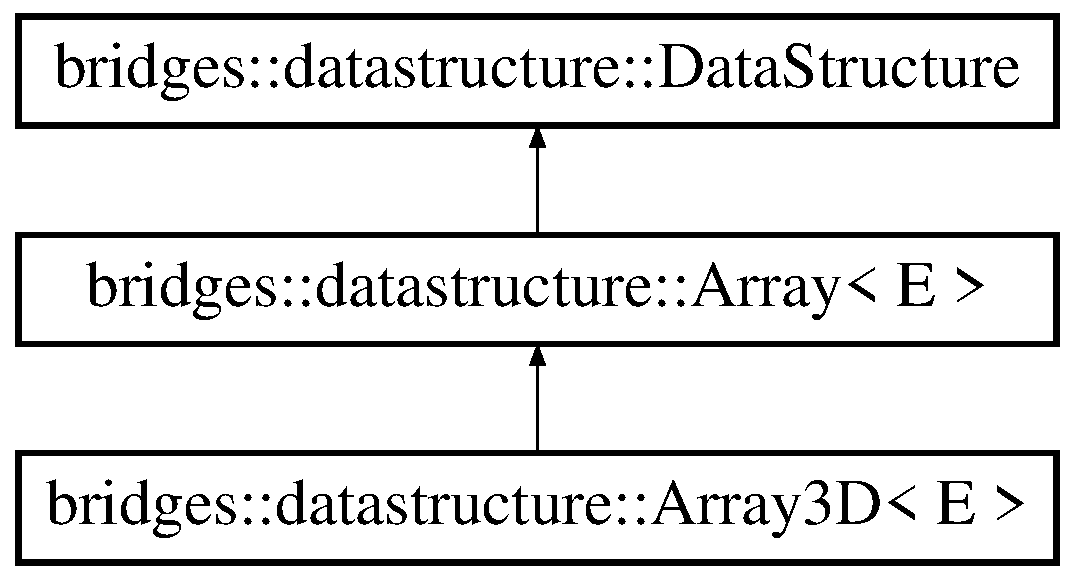
\includegraphics[height=3.000000cm]{classbridges_1_1datastructure_1_1_array3_d}
\end{center}
\end{figure}


\subsection{Detailed Description}
\subsubsection*{template$<$typename E$>$\newline
class bridges\+::datastructure\+::\+Array3\+D$<$ E $>$}

A B\+R\+I\+D\+G\+ES array type. 

This class can be used to create 3D arrays of any type.

The access to the values stored are done directly using bracket operators such as


\begin{DoxyCode}{0}
\DoxyCodeLine{Array3D<std::string> arr(19, 30, 30);}
\DoxyCodeLine{arr [12][25][12] = \textcolor{stringliteral}{"hello!"};}
\end{DoxyCode}


Entries in the array can be styled by showing a label and changing the color of an entry. This is achieved by styling the underlying element to a particular entry of the array such as\+:


\begin{DoxyCode}{0}
\DoxyCodeLine{Array3D<std::string> arr(19, 30, 3);}
\DoxyCodeLine{arr.getElement(12, 25, 0).setColor(\textcolor{stringliteral}{"yellow"});}
\DoxyCodeLine{arr.getElement(12, 25, 2).setLabel(\textcolor{stringliteral}{"Hi there"});}
\end{DoxyCode}


\begin{DoxySeeAlso}{See also}
See tutorial at\+: \href{http://bridgesuncc.github.io/tutorials/Array.html}{\texttt{ http\+://bridgesuncc.\+github.\+io/tutorials/\+Array.\+html}}
\end{DoxySeeAlso}

\begin{DoxyParams}{Parameters}
{\em E} & the application data type\\
\hline
\end{DoxyParams}
\begin{DoxyAuthor}{Author}
Kalpathi Subramanian 
\end{DoxyAuthor}
\begin{DoxyDate}{Date}
7/16/19 
\end{DoxyDate}
\subsection*{Classes}
\begin{DoxyCompactItemize}
\item 
struct \mbox{\hyperlink{structbridges_1_1datastructure_1_1_array3_d_1_1_bracket__helper}{Bracket\+\_\+helper}}
\begin{DoxyCompactList}\small\item\em helper class to make \mbox{[}\mbox{]}\mbox{[}\mbox{]} operators work on array 2d. You should never use it directly \end{DoxyCompactList}\item 
struct \mbox{\hyperlink{structbridges_1_1datastructure_1_1_array3_d_1_1_bracket__helper2}{Bracket\+\_\+helper2}}
\item 
struct \mbox{\hyperlink{structbridges_1_1datastructure_1_1_array3_d_1_1_bracket__helper2__const}{Bracket\+\_\+helper2\+\_\+const}}
\item 
struct \mbox{\hyperlink{structbridges_1_1datastructure_1_1_array3_d_1_1_bracket__helper__const}{Bracket\+\_\+helper\+\_\+const}}
\begin{DoxyCompactList}\small\item\em helper class to make \mbox{[}\mbox{]}\mbox{[}\mbox{]} operators work on array 2d. You should never use it directly \end{DoxyCompactList}\end{DoxyCompactItemize}
\subsection*{Public Member Functions}
\begin{DoxyCompactItemize}
\item 
virtual \mbox{\hyperlink{classbridges_1_1datastructure_1_1_array3_d_afad3212fe6c2954859a7ea6dce7a739c}{$\sim$\+Array3D}} ()
\item 
\mbox{\hyperlink{classbridges_1_1datastructure_1_1_array3_d_af2d55bb9cf9057b9d5af4a24c6dc3173}{Array3D}} (int slices, int rows, int columns)
\item 
int \mbox{\hyperlink{classbridges_1_1datastructure_1_1_array3_d_a73aebe1098512ca4196cb8da0eb493fe}{get\+Num\+Rows}} ()
\item 
int \mbox{\hyperlink{classbridges_1_1datastructure_1_1_array3_d_acbd00c0c4448ff7ff03c76bc0701f602}{get\+Num\+Columns}} ()
\item 
int \mbox{\hyperlink{classbridges_1_1datastructure_1_1_array3_d_ad2fb0a0b8be702944c25b6fc807263f7}{get\+Num\+Slices}} ()
\item 
\mbox{\hyperlink{classbridges_1_1datastructure_1_1_element}{Element}}$<$ E $>$ \& \mbox{\hyperlink{classbridges_1_1datastructure_1_1_array3_d_a1e4a2bea4f3a292289cfc0a4d530108f}{get\+Element}} (int slice, int row, int col)
\item 
\mbox{\hyperlink{classbridges_1_1datastructure_1_1_element}{Element}}$<$ E $>$ const  \& \mbox{\hyperlink{classbridges_1_1datastructure_1_1_array3_d_a8f9d33a89196ef13839f30334b25476d}{get\+Element}} (int slice, int row, int col) const
\item 
void \mbox{\hyperlink{classbridges_1_1datastructure_1_1_array3_d_aaad4c68544d51cade79f318230ab2bcf}{set\+Element}} (int slice, int row, int col, \mbox{\hyperlink{classbridges_1_1datastructure_1_1_element}{Element}}$<$ E $>$ el)
\item 
\mbox{\hyperlink{structbridges_1_1datastructure_1_1_array3_d_1_1_bracket__helper}{Bracket\+\_\+helper}} \mbox{\hyperlink{classbridges_1_1datastructure_1_1_array3_d_a0b285b00e5d152d2968bee6b3aaf9349}{operator\mbox{[}$\,$\mbox{]}}} (int index)
\begin{DoxyCompactList}\small\item\em enables using the bracket \mbox{[}\mbox{]} operator \end{DoxyCompactList}\item 
\mbox{\hyperlink{structbridges_1_1datastructure_1_1_array3_d_1_1_bracket__helper__const}{Bracket\+\_\+helper\+\_\+const}} \mbox{\hyperlink{classbridges_1_1datastructure_1_1_array3_d_acfc0446c919e7ca70cc31d0624b3bcd1}{operator\mbox{[}$\,$\mbox{]}}} (int index) const
\begin{DoxyCompactList}\small\item\em enables using the bracket \mbox{[}\mbox{]} operator \end{DoxyCompactList}\end{DoxyCompactItemize}
\subsection*{Additional Inherited Members}


\subsection{Constructor \& Destructor Documentation}
\mbox{\Hypertarget{classbridges_1_1datastructure_1_1_array3_d_afad3212fe6c2954859a7ea6dce7a739c}\label{classbridges_1_1datastructure_1_1_array3_d_afad3212fe6c2954859a7ea6dce7a739c}} 
\index{bridges::datastructure::Array3D$<$ E $>$@{bridges::datastructure::Array3D$<$ E $>$}!````~Array3D@{$\sim$Array3D}}
\index{````~Array3D@{$\sim$Array3D}!bridges::datastructure::Array3D$<$ E $>$@{bridges::datastructure::Array3D$<$ E $>$}}
\subsubsection{\texorpdfstring{$\sim$Array3D()}{~Array3D()}}
{\footnotesize\ttfamily template$<$typename E$>$ \\
virtual \mbox{\hyperlink{classbridges_1_1datastructure_1_1_array3_d}{bridges\+::datastructure\+::\+Array3D}}$<$ E $>$\+::$\sim$\mbox{\hyperlink{classbridges_1_1datastructure_1_1_array3_d}{Array3D}} (\begin{DoxyParamCaption}{ }\end{DoxyParamCaption})\hspace{0.3cm}{\ttfamily [inline]}, {\ttfamily [virtual]}}

\mbox{\Hypertarget{classbridges_1_1datastructure_1_1_array3_d_af2d55bb9cf9057b9d5af4a24c6dc3173}\label{classbridges_1_1datastructure_1_1_array3_d_af2d55bb9cf9057b9d5af4a24c6dc3173}} 
\index{bridges::datastructure::Array3D$<$ E $>$@{bridges::datastructure::Array3D$<$ E $>$}!Array3D@{Array3D}}
\index{Array3D@{Array3D}!bridges::datastructure::Array3D$<$ E $>$@{bridges::datastructure::Array3D$<$ E $>$}}
\subsubsection{\texorpdfstring{Array3D()}{Array3D()}}
{\footnotesize\ttfamily template$<$typename E$>$ \\
\mbox{\hyperlink{classbridges_1_1datastructure_1_1_array3_d}{bridges\+::datastructure\+::\+Array3D}}$<$ E $>$\+::\mbox{\hyperlink{classbridges_1_1datastructure_1_1_array3_d}{Array3D}} (\begin{DoxyParamCaption}\item[{int}]{slices,  }\item[{int}]{rows,  }\item[{int}]{columns }\end{DoxyParamCaption})\hspace{0.3cm}{\ttfamily [inline]}}

builds a 3D array. 
\begin{DoxyParams}{Parameters}
{\em cols} & number of columns \\
\hline
{\em rows} & number of rows \\
\hline
{\em slices} & number of slices \\
\hline
\end{DoxyParams}


\subsection{Member Function Documentation}
\mbox{\Hypertarget{classbridges_1_1datastructure_1_1_array3_d_a1e4a2bea4f3a292289cfc0a4d530108f}\label{classbridges_1_1datastructure_1_1_array3_d_a1e4a2bea4f3a292289cfc0a4d530108f}} 
\index{bridges::datastructure::Array3D$<$ E $>$@{bridges::datastructure::Array3D$<$ E $>$}!getElement@{getElement}}
\index{getElement@{getElement}!bridges::datastructure::Array3D$<$ E $>$@{bridges::datastructure::Array3D$<$ E $>$}}
\subsubsection{\texorpdfstring{getElement()}{getElement()}\hspace{0.1cm}{\footnotesize\ttfamily [1/2]}}
{\footnotesize\ttfamily template$<$typename E$>$ \\
\mbox{\hyperlink{classbridges_1_1datastructure_1_1_element}{Element}}$<$E$>$\& \mbox{\hyperlink{classbridges_1_1datastructure_1_1_array3_d}{bridges\+::datastructure\+::\+Array3D}}$<$ E $>$\+::get\+Element (\begin{DoxyParamCaption}\item[{int}]{slice,  }\item[{int}]{row,  }\item[{int}]{col }\end{DoxyParamCaption})\hspace{0.3cm}{\ttfamily [inline]}}

Get the object at (slice, row, col) for 3D arrays


\begin{DoxyParams}{Parameters}
{\em slice} & -\/ slice index \\
\hline
{\em row} & -\/ row index \\
\hline
{\em col} & -\/ column index\\
\hline
\end{DoxyParams}
\begin{DoxyReturn}{Returns}
Element$<$\+E$>$ object at slice, row, col 
\end{DoxyReturn}
\mbox{\Hypertarget{classbridges_1_1datastructure_1_1_array3_d_a8f9d33a89196ef13839f30334b25476d}\label{classbridges_1_1datastructure_1_1_array3_d_a8f9d33a89196ef13839f30334b25476d}} 
\index{bridges::datastructure::Array3D$<$ E $>$@{bridges::datastructure::Array3D$<$ E $>$}!getElement@{getElement}}
\index{getElement@{getElement}!bridges::datastructure::Array3D$<$ E $>$@{bridges::datastructure::Array3D$<$ E $>$}}
\subsubsection{\texorpdfstring{getElement()}{getElement()}\hspace{0.1cm}{\footnotesize\ttfamily [2/2]}}
{\footnotesize\ttfamily template$<$typename E$>$ \\
\mbox{\hyperlink{classbridges_1_1datastructure_1_1_element}{Element}}$<$E$>$ const\& \mbox{\hyperlink{classbridges_1_1datastructure_1_1_array3_d}{bridges\+::datastructure\+::\+Array3D}}$<$ E $>$\+::get\+Element (\begin{DoxyParamCaption}\item[{int}]{slice,  }\item[{int}]{row,  }\item[{int}]{col }\end{DoxyParamCaption}) const\hspace{0.3cm}{\ttfamily [inline]}}

Get the object at (slice, rows, col) for 3D arrays


\begin{DoxyParams}{Parameters}
{\em col} & column index \\
\hline
{\em row} & row index \\
\hline
{\em slice} & slice index\\
\hline
\end{DoxyParams}
\begin{DoxyReturn}{Returns}
the \mbox{\hyperlink{classbridges_1_1datastructure_1_1_element}{Element}} at (slice, rows, col) 
\end{DoxyReturn}
\mbox{\Hypertarget{classbridges_1_1datastructure_1_1_array3_d_acbd00c0c4448ff7ff03c76bc0701f602}\label{classbridges_1_1datastructure_1_1_array3_d_acbd00c0c4448ff7ff03c76bc0701f602}} 
\index{bridges::datastructure::Array3D$<$ E $>$@{bridges::datastructure::Array3D$<$ E $>$}!getNumColumns@{getNumColumns}}
\index{getNumColumns@{getNumColumns}!bridges::datastructure::Array3D$<$ E $>$@{bridges::datastructure::Array3D$<$ E $>$}}
\subsubsection{\texorpdfstring{getNumColumns()}{getNumColumns()}}
{\footnotesize\ttfamily template$<$typename E$>$ \\
int \mbox{\hyperlink{classbridges_1_1datastructure_1_1_array3_d}{bridges\+::datastructure\+::\+Array3D}}$<$ E $>$\+::get\+Num\+Columns (\begin{DoxyParamCaption}{ }\end{DoxyParamCaption})\hspace{0.3cm}{\ttfamily [inline]}}

Gets the number of columns of the 3D array \begin{DoxyReturn}{Returns}
number of columns 
\end{DoxyReturn}
\mbox{\Hypertarget{classbridges_1_1datastructure_1_1_array3_d_a73aebe1098512ca4196cb8da0eb493fe}\label{classbridges_1_1datastructure_1_1_array3_d_a73aebe1098512ca4196cb8da0eb493fe}} 
\index{bridges::datastructure::Array3D$<$ E $>$@{bridges::datastructure::Array3D$<$ E $>$}!getNumRows@{getNumRows}}
\index{getNumRows@{getNumRows}!bridges::datastructure::Array3D$<$ E $>$@{bridges::datastructure::Array3D$<$ E $>$}}
\subsubsection{\texorpdfstring{getNumRows()}{getNumRows()}}
{\footnotesize\ttfamily template$<$typename E$>$ \\
int \mbox{\hyperlink{classbridges_1_1datastructure_1_1_array3_d}{bridges\+::datastructure\+::\+Array3D}}$<$ E $>$\+::get\+Num\+Rows (\begin{DoxyParamCaption}{ }\end{DoxyParamCaption})\hspace{0.3cm}{\ttfamily [inline]}}

Gets the number of rows of the 3D array \begin{DoxyReturn}{Returns}
number of rows 
\end{DoxyReturn}
\mbox{\Hypertarget{classbridges_1_1datastructure_1_1_array3_d_ad2fb0a0b8be702944c25b6fc807263f7}\label{classbridges_1_1datastructure_1_1_array3_d_ad2fb0a0b8be702944c25b6fc807263f7}} 
\index{bridges::datastructure::Array3D$<$ E $>$@{bridges::datastructure::Array3D$<$ E $>$}!getNumSlices@{getNumSlices}}
\index{getNumSlices@{getNumSlices}!bridges::datastructure::Array3D$<$ E $>$@{bridges::datastructure::Array3D$<$ E $>$}}
\subsubsection{\texorpdfstring{getNumSlices()}{getNumSlices()}}
{\footnotesize\ttfamily template$<$typename E$>$ \\
int \mbox{\hyperlink{classbridges_1_1datastructure_1_1_array3_d}{bridges\+::datastructure\+::\+Array3D}}$<$ E $>$\+::get\+Num\+Slices (\begin{DoxyParamCaption}{ }\end{DoxyParamCaption})\hspace{0.3cm}{\ttfamily [inline]}}

Gets the number of slices of the 3D array \begin{DoxyReturn}{Returns}
number of slices 
\end{DoxyReturn}
\mbox{\Hypertarget{classbridges_1_1datastructure_1_1_array3_d_a0b285b00e5d152d2968bee6b3aaf9349}\label{classbridges_1_1datastructure_1_1_array3_d_a0b285b00e5d152d2968bee6b3aaf9349}} 
\index{bridges::datastructure::Array3D$<$ E $>$@{bridges::datastructure::Array3D$<$ E $>$}!operator\mbox{[}\mbox{]}@{operator[]}}
\index{operator\mbox{[}\mbox{]}@{operator[]}!bridges::datastructure::Array3D$<$ E $>$@{bridges::datastructure::Array3D$<$ E $>$}}
\subsubsection{\texorpdfstring{operator[]()}{operator[]()}\hspace{0.1cm}{\footnotesize\ttfamily [1/2]}}
{\footnotesize\ttfamily template$<$typename E$>$ \\
\mbox{\hyperlink{structbridges_1_1datastructure_1_1_array3_d_1_1_bracket__helper}{Bracket\+\_\+helper}} \mbox{\hyperlink{classbridges_1_1datastructure_1_1_array3_d}{bridges\+::datastructure\+::\+Array3D}}$<$ E $>$\+::operator\mbox{[}$\,$\mbox{]} (\begin{DoxyParamCaption}\item[{int}]{index }\end{DoxyParamCaption})\hspace{0.3cm}{\ttfamily [inline]}}



enables using the bracket \mbox{[}\mbox{]} operator 

\mbox{\Hypertarget{classbridges_1_1datastructure_1_1_array3_d_acfc0446c919e7ca70cc31d0624b3bcd1}\label{classbridges_1_1datastructure_1_1_array3_d_acfc0446c919e7ca70cc31d0624b3bcd1}} 
\index{bridges::datastructure::Array3D$<$ E $>$@{bridges::datastructure::Array3D$<$ E $>$}!operator\mbox{[}\mbox{]}@{operator[]}}
\index{operator\mbox{[}\mbox{]}@{operator[]}!bridges::datastructure::Array3D$<$ E $>$@{bridges::datastructure::Array3D$<$ E $>$}}
\subsubsection{\texorpdfstring{operator[]()}{operator[]()}\hspace{0.1cm}{\footnotesize\ttfamily [2/2]}}
{\footnotesize\ttfamily template$<$typename E$>$ \\
\mbox{\hyperlink{structbridges_1_1datastructure_1_1_array3_d_1_1_bracket__helper__const}{Bracket\+\_\+helper\+\_\+const}} \mbox{\hyperlink{classbridges_1_1datastructure_1_1_array3_d}{bridges\+::datastructure\+::\+Array3D}}$<$ E $>$\+::operator\mbox{[}$\,$\mbox{]} (\begin{DoxyParamCaption}\item[{int}]{index }\end{DoxyParamCaption}) const\hspace{0.3cm}{\ttfamily [inline]}}



enables using the bracket \mbox{[}\mbox{]} operator 

\mbox{\Hypertarget{classbridges_1_1datastructure_1_1_array3_d_aaad4c68544d51cade79f318230ab2bcf}\label{classbridges_1_1datastructure_1_1_array3_d_aaad4c68544d51cade79f318230ab2bcf}} 
\index{bridges::datastructure::Array3D$<$ E $>$@{bridges::datastructure::Array3D$<$ E $>$}!setElement@{setElement}}
\index{setElement@{setElement}!bridges::datastructure::Array3D$<$ E $>$@{bridges::datastructure::Array3D$<$ E $>$}}
\subsubsection{\texorpdfstring{setElement()}{setElement()}}
{\footnotesize\ttfamily template$<$typename E$>$ \\
void \mbox{\hyperlink{classbridges_1_1datastructure_1_1_array3_d}{bridges\+::datastructure\+::\+Array3D}}$<$ E $>$\+::set\+Element (\begin{DoxyParamCaption}\item[{int}]{slice,  }\item[{int}]{row,  }\item[{int}]{col,  }\item[{\mbox{\hyperlink{classbridges_1_1datastructure_1_1_element}{Element}}$<$ E $>$}]{el }\end{DoxyParamCaption})\hspace{0.3cm}{\ttfamily [inline]}}

Set the object at index slice, row, col -\/ 3D array


\begin{DoxyParams}{Parameters}
{\em slice} & slice index into the array \\
\hline
{\em col} & column index into the array \\
\hline
{\em row} & row index into the array \\
\hline
{\em el} & -\/ \mbox{\hyperlink{classbridges_1_1datastructure_1_1_element}{Element}} object \\
\hline
\end{DoxyParams}


The documentation for this class was generated from the following file\+:\begin{DoxyCompactItemize}
\item 
/\+Users/kalpathi/gr/bridges/cxx/src/\mbox{\hyperlink{_array3_d_8h}{Array3\+D.\+h}}\end{DoxyCompactItemize}

\hypertarget{classsio_1_1array__message}{}\doxysection{sio\+::array\+\_\+message Class Reference}
\label{classsio_1_1array__message}\index{sio::array\_message@{sio::array\_message}}


{\ttfamily \#include $<$sio\+\_\+message.\+h$>$}

Inheritance diagram for sio\+::array\+\_\+message\+:\begin{figure}[H]
\begin{center}
\leavevmode
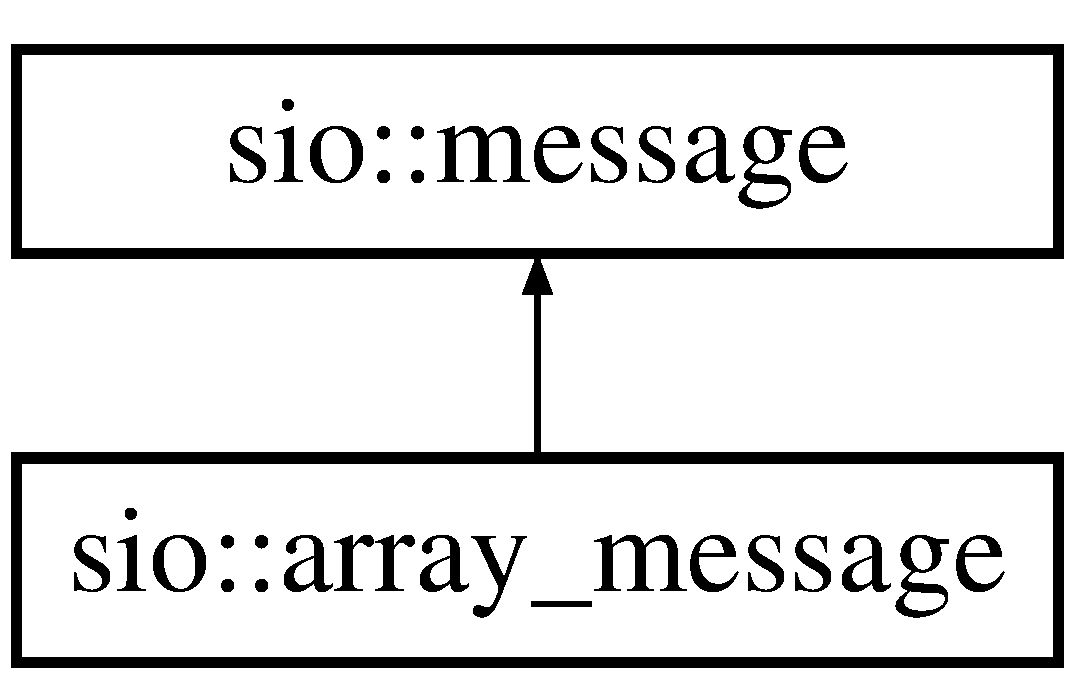
\includegraphics[height=2.000000cm]{classsio_1_1array__message}
\end{center}
\end{figure}
\doxysubsection*{Public Member Functions}
\begin{DoxyCompactItemize}
\item 
void \mbox{\hyperlink{classsio_1_1array__message_a2bb6a7dc5a4bc481ec6638b027732e30}{push}} (\mbox{\hyperlink{classsio_1_1message_a6340b6fef57e4516eb17928b1885a615}{message\+::ptr}} const \&\mbox{\hyperlink{classsio_1_1message}{message}})
\item 
void \mbox{\hyperlink{classsio_1_1array__message_aa64e942b4bcdd9484638666bb45b6a1c}{push}} (const std\+::string \&text)
\item 
void \mbox{\hyperlink{classsio_1_1array__message_acf436faa854bfa7c3e323beea308a1a5}{push}} (std\+::string \&\&text)
\item 
void \mbox{\hyperlink{classsio_1_1array__message_a52d0cd50d5cd438ae21ddfbf2c62b72d}{push}} (std\+::shared\+\_\+ptr$<$ std\+::string $>$ const \&binary)
\item 
void \mbox{\hyperlink{classsio_1_1array__message_ab69517653493458d697647e1b5e0ae3f}{push}} (std\+::shared\+\_\+ptr$<$ const std\+::string $>$ const \&binary)
\item 
void \mbox{\hyperlink{classsio_1_1array__message_a5bf35c4605d386ca824c0948d991bed2}{insert}} (size\+\_\+t pos, \mbox{\hyperlink{classsio_1_1message_a6340b6fef57e4516eb17928b1885a615}{message\+::ptr}} const \&\mbox{\hyperlink{classsio_1_1message}{message}})
\item 
void \mbox{\hyperlink{classsio_1_1array__message_a6c42d79eee6b499ffd08769c741d5b7f}{insert}} (size\+\_\+t pos, const std\+::string \&text)
\item 
void \mbox{\hyperlink{classsio_1_1array__message_a0f865c08b9da48112d4b7c628f851220}{insert}} (size\+\_\+t pos, std\+::string \&\&text)
\item 
void \mbox{\hyperlink{classsio_1_1array__message_ac84632e5968cc80be47314a00c17af0c}{insert}} (size\+\_\+t pos, std\+::shared\+\_\+ptr$<$ std\+::string $>$ const \&binary)
\item 
void \mbox{\hyperlink{classsio_1_1array__message_ae154a195d738a3dec30a78865598ce89}{insert}} (size\+\_\+t pos, std\+::shared\+\_\+ptr$<$ const std\+::string $>$ const \&binary)
\item 
size\+\_\+t \mbox{\hyperlink{classsio_1_1array__message_ae854fb58883883ccc930de77285d7dae}{size}} () const
\item 
const \mbox{\hyperlink{classsio_1_1message_a6340b6fef57e4516eb17928b1885a615}{message\+::ptr}} \& \mbox{\hyperlink{classsio_1_1array__message_a97aba94eb40546998c86ed6901a8f331}{at}} (size\+\_\+t i) const
\item 
const \mbox{\hyperlink{classsio_1_1message_a6340b6fef57e4516eb17928b1885a615}{message\+::ptr}} \& \mbox{\hyperlink{classsio_1_1array__message_a4643f17c6f0fca23cd8c2c1d359d362d}{operator\mbox{[}$\,$\mbox{]}}} (size\+\_\+t i) const
\item 
std\+::vector$<$ \mbox{\hyperlink{classsio_1_1message_a6340b6fef57e4516eb17928b1885a615}{ptr}} $>$ \& \mbox{\hyperlink{classsio_1_1array__message_a7d039c4e78bb01f5e19921e0f09509c2}{get\+\_\+vector}} ()
\item 
const std\+::vector$<$ \mbox{\hyperlink{classsio_1_1message_a6340b6fef57e4516eb17928b1885a615}{ptr}} $>$ \& \mbox{\hyperlink{classsio_1_1array__message_a298e6b4d041e95ac5b90cdff6fdef5fb}{get\+\_\+vector}} () const
\end{DoxyCompactItemize}
\doxysubsection*{Static Public Member Functions}
\begin{DoxyCompactItemize}
\item 
static \mbox{\hyperlink{classsio_1_1message_a6340b6fef57e4516eb17928b1885a615}{message\+::ptr}} \mbox{\hyperlink{classsio_1_1array__message_ae39847edc10bcfc748257485a57382f5}{create}} ()
\end{DoxyCompactItemize}
\doxysubsection*{Additional Inherited Members}


\doxysubsection{Member Function Documentation}
\mbox{\Hypertarget{classsio_1_1array__message_a97aba94eb40546998c86ed6901a8f331}\label{classsio_1_1array__message_a97aba94eb40546998c86ed6901a8f331}} 
\index{sio::array\_message@{sio::array\_message}!at@{at}}
\index{at@{at}!sio::array\_message@{sio::array\_message}}
\doxysubsubsection{\texorpdfstring{at()}{at()}}
{\footnotesize\ttfamily const \mbox{\hyperlink{classsio_1_1message_a6340b6fef57e4516eb17928b1885a615}{message\+::ptr}}\& sio\+::array\+\_\+message\+::at (\begin{DoxyParamCaption}\item[{size\+\_\+t}]{i }\end{DoxyParamCaption}) const\hspace{0.3cm}{\ttfamily [inline]}}

\mbox{\Hypertarget{classsio_1_1array__message_ae39847edc10bcfc748257485a57382f5}\label{classsio_1_1array__message_ae39847edc10bcfc748257485a57382f5}} 
\index{sio::array\_message@{sio::array\_message}!create@{create}}
\index{create@{create}!sio::array\_message@{sio::array\_message}}
\doxysubsubsection{\texorpdfstring{create()}{create()}}
{\footnotesize\ttfamily static \mbox{\hyperlink{classsio_1_1message_a6340b6fef57e4516eb17928b1885a615}{message\+::ptr}} sio\+::array\+\_\+message\+::create (\begin{DoxyParamCaption}{ }\end{DoxyParamCaption})\hspace{0.3cm}{\ttfamily [inline]}, {\ttfamily [static]}}

\mbox{\Hypertarget{classsio_1_1array__message_a7d039c4e78bb01f5e19921e0f09509c2}\label{classsio_1_1array__message_a7d039c4e78bb01f5e19921e0f09509c2}} 
\index{sio::array\_message@{sio::array\_message}!get\_vector@{get\_vector}}
\index{get\_vector@{get\_vector}!sio::array\_message@{sio::array\_message}}
\doxysubsubsection{\texorpdfstring{get\_vector()}{get\_vector()}\hspace{0.1cm}{\footnotesize\ttfamily [1/2]}}
{\footnotesize\ttfamily std\+::vector$<$\mbox{\hyperlink{classsio_1_1message_a6340b6fef57e4516eb17928b1885a615}{ptr}}$>$\& sio\+::array\+\_\+message\+::get\+\_\+vector (\begin{DoxyParamCaption}{ }\end{DoxyParamCaption})\hspace{0.3cm}{\ttfamily [inline]}, {\ttfamily [virtual]}}



Reimplemented from \mbox{\hyperlink{classsio_1_1message_af62004da998c98ee7039a26d809c44d3}{sio\+::message}}.

\mbox{\Hypertarget{classsio_1_1array__message_a298e6b4d041e95ac5b90cdff6fdef5fb}\label{classsio_1_1array__message_a298e6b4d041e95ac5b90cdff6fdef5fb}} 
\index{sio::array\_message@{sio::array\_message}!get\_vector@{get\_vector}}
\index{get\_vector@{get\_vector}!sio::array\_message@{sio::array\_message}}
\doxysubsubsection{\texorpdfstring{get\_vector()}{get\_vector()}\hspace{0.1cm}{\footnotesize\ttfamily [2/2]}}
{\footnotesize\ttfamily const std\+::vector$<$\mbox{\hyperlink{classsio_1_1message_a6340b6fef57e4516eb17928b1885a615}{ptr}}$>$\& sio\+::array\+\_\+message\+::get\+\_\+vector (\begin{DoxyParamCaption}{ }\end{DoxyParamCaption}) const\hspace{0.3cm}{\ttfamily [inline]}, {\ttfamily [virtual]}}



Reimplemented from \mbox{\hyperlink{classsio_1_1message_af310192e16427f655dc89c627aae4fe7}{sio\+::message}}.

\mbox{\Hypertarget{classsio_1_1array__message_a6c42d79eee6b499ffd08769c741d5b7f}\label{classsio_1_1array__message_a6c42d79eee6b499ffd08769c741d5b7f}} 
\index{sio::array\_message@{sio::array\_message}!insert@{insert}}
\index{insert@{insert}!sio::array\_message@{sio::array\_message}}
\doxysubsubsection{\texorpdfstring{insert()}{insert()}\hspace{0.1cm}{\footnotesize\ttfamily [1/5]}}
{\footnotesize\ttfamily void sio\+::array\+\_\+message\+::insert (\begin{DoxyParamCaption}\item[{size\+\_\+t}]{pos,  }\item[{const std\+::string \&}]{text }\end{DoxyParamCaption})\hspace{0.3cm}{\ttfamily [inline]}}

\mbox{\Hypertarget{classsio_1_1array__message_a5bf35c4605d386ca824c0948d991bed2}\label{classsio_1_1array__message_a5bf35c4605d386ca824c0948d991bed2}} 
\index{sio::array\_message@{sio::array\_message}!insert@{insert}}
\index{insert@{insert}!sio::array\_message@{sio::array\_message}}
\doxysubsubsection{\texorpdfstring{insert()}{insert()}\hspace{0.1cm}{\footnotesize\ttfamily [2/5]}}
{\footnotesize\ttfamily void sio\+::array\+\_\+message\+::insert (\begin{DoxyParamCaption}\item[{size\+\_\+t}]{pos,  }\item[{\mbox{\hyperlink{classsio_1_1message_a6340b6fef57e4516eb17928b1885a615}{message\+::ptr}} const \&}]{message }\end{DoxyParamCaption})\hspace{0.3cm}{\ttfamily [inline]}}

\mbox{\Hypertarget{classsio_1_1array__message_ae154a195d738a3dec30a78865598ce89}\label{classsio_1_1array__message_ae154a195d738a3dec30a78865598ce89}} 
\index{sio::array\_message@{sio::array\_message}!insert@{insert}}
\index{insert@{insert}!sio::array\_message@{sio::array\_message}}
\doxysubsubsection{\texorpdfstring{insert()}{insert()}\hspace{0.1cm}{\footnotesize\ttfamily [3/5]}}
{\footnotesize\ttfamily void sio\+::array\+\_\+message\+::insert (\begin{DoxyParamCaption}\item[{size\+\_\+t}]{pos,  }\item[{std\+::shared\+\_\+ptr$<$ const std\+::string $>$ const \&}]{binary }\end{DoxyParamCaption})\hspace{0.3cm}{\ttfamily [inline]}}

\mbox{\Hypertarget{classsio_1_1array__message_ac84632e5968cc80be47314a00c17af0c}\label{classsio_1_1array__message_ac84632e5968cc80be47314a00c17af0c}} 
\index{sio::array\_message@{sio::array\_message}!insert@{insert}}
\index{insert@{insert}!sio::array\_message@{sio::array\_message}}
\doxysubsubsection{\texorpdfstring{insert()}{insert()}\hspace{0.1cm}{\footnotesize\ttfamily [4/5]}}
{\footnotesize\ttfamily void sio\+::array\+\_\+message\+::insert (\begin{DoxyParamCaption}\item[{size\+\_\+t}]{pos,  }\item[{std\+::shared\+\_\+ptr$<$ std\+::string $>$ const \&}]{binary }\end{DoxyParamCaption})\hspace{0.3cm}{\ttfamily [inline]}}

\mbox{\Hypertarget{classsio_1_1array__message_a0f865c08b9da48112d4b7c628f851220}\label{classsio_1_1array__message_a0f865c08b9da48112d4b7c628f851220}} 
\index{sio::array\_message@{sio::array\_message}!insert@{insert}}
\index{insert@{insert}!sio::array\_message@{sio::array\_message}}
\doxysubsubsection{\texorpdfstring{insert()}{insert()}\hspace{0.1cm}{\footnotesize\ttfamily [5/5]}}
{\footnotesize\ttfamily void sio\+::array\+\_\+message\+::insert (\begin{DoxyParamCaption}\item[{size\+\_\+t}]{pos,  }\item[{std\+::string \&\&}]{text }\end{DoxyParamCaption})\hspace{0.3cm}{\ttfamily [inline]}}

\mbox{\Hypertarget{classsio_1_1array__message_a4643f17c6f0fca23cd8c2c1d359d362d}\label{classsio_1_1array__message_a4643f17c6f0fca23cd8c2c1d359d362d}} 
\index{sio::array\_message@{sio::array\_message}!operator\mbox{[}\mbox{]}@{operator[]}}
\index{operator\mbox{[}\mbox{]}@{operator[]}!sio::array\_message@{sio::array\_message}}
\doxysubsubsection{\texorpdfstring{operator[]()}{operator[]()}}
{\footnotesize\ttfamily const \mbox{\hyperlink{classsio_1_1message_a6340b6fef57e4516eb17928b1885a615}{message\+::ptr}}\& sio\+::array\+\_\+message\+::operator\mbox{[}$\,$\mbox{]} (\begin{DoxyParamCaption}\item[{size\+\_\+t}]{i }\end{DoxyParamCaption}) const\hspace{0.3cm}{\ttfamily [inline]}}

\mbox{\Hypertarget{classsio_1_1array__message_aa64e942b4bcdd9484638666bb45b6a1c}\label{classsio_1_1array__message_aa64e942b4bcdd9484638666bb45b6a1c}} 
\index{sio::array\_message@{sio::array\_message}!push@{push}}
\index{push@{push}!sio::array\_message@{sio::array\_message}}
\doxysubsubsection{\texorpdfstring{push()}{push()}\hspace{0.1cm}{\footnotesize\ttfamily [1/5]}}
{\footnotesize\ttfamily void sio\+::array\+\_\+message\+::push (\begin{DoxyParamCaption}\item[{const std\+::string \&}]{text }\end{DoxyParamCaption})\hspace{0.3cm}{\ttfamily [inline]}}

\mbox{\Hypertarget{classsio_1_1array__message_a2bb6a7dc5a4bc481ec6638b027732e30}\label{classsio_1_1array__message_a2bb6a7dc5a4bc481ec6638b027732e30}} 
\index{sio::array\_message@{sio::array\_message}!push@{push}}
\index{push@{push}!sio::array\_message@{sio::array\_message}}
\doxysubsubsection{\texorpdfstring{push()}{push()}\hspace{0.1cm}{\footnotesize\ttfamily [2/5]}}
{\footnotesize\ttfamily void sio\+::array\+\_\+message\+::push (\begin{DoxyParamCaption}\item[{\mbox{\hyperlink{classsio_1_1message_a6340b6fef57e4516eb17928b1885a615}{message\+::ptr}} const \&}]{message }\end{DoxyParamCaption})\hspace{0.3cm}{\ttfamily [inline]}}

\mbox{\Hypertarget{classsio_1_1array__message_ab69517653493458d697647e1b5e0ae3f}\label{classsio_1_1array__message_ab69517653493458d697647e1b5e0ae3f}} 
\index{sio::array\_message@{sio::array\_message}!push@{push}}
\index{push@{push}!sio::array\_message@{sio::array\_message}}
\doxysubsubsection{\texorpdfstring{push()}{push()}\hspace{0.1cm}{\footnotesize\ttfamily [3/5]}}
{\footnotesize\ttfamily void sio\+::array\+\_\+message\+::push (\begin{DoxyParamCaption}\item[{std\+::shared\+\_\+ptr$<$ const std\+::string $>$ const \&}]{binary }\end{DoxyParamCaption})\hspace{0.3cm}{\ttfamily [inline]}}

\mbox{\Hypertarget{classsio_1_1array__message_a52d0cd50d5cd438ae21ddfbf2c62b72d}\label{classsio_1_1array__message_a52d0cd50d5cd438ae21ddfbf2c62b72d}} 
\index{sio::array\_message@{sio::array\_message}!push@{push}}
\index{push@{push}!sio::array\_message@{sio::array\_message}}
\doxysubsubsection{\texorpdfstring{push()}{push()}\hspace{0.1cm}{\footnotesize\ttfamily [4/5]}}
{\footnotesize\ttfamily void sio\+::array\+\_\+message\+::push (\begin{DoxyParamCaption}\item[{std\+::shared\+\_\+ptr$<$ std\+::string $>$ const \&}]{binary }\end{DoxyParamCaption})\hspace{0.3cm}{\ttfamily [inline]}}

\mbox{\Hypertarget{classsio_1_1array__message_acf436faa854bfa7c3e323beea308a1a5}\label{classsio_1_1array__message_acf436faa854bfa7c3e323beea308a1a5}} 
\index{sio::array\_message@{sio::array\_message}!push@{push}}
\index{push@{push}!sio::array\_message@{sio::array\_message}}
\doxysubsubsection{\texorpdfstring{push()}{push()}\hspace{0.1cm}{\footnotesize\ttfamily [5/5]}}
{\footnotesize\ttfamily void sio\+::array\+\_\+message\+::push (\begin{DoxyParamCaption}\item[{std\+::string \&\&}]{text }\end{DoxyParamCaption})\hspace{0.3cm}{\ttfamily [inline]}}

\mbox{\Hypertarget{classsio_1_1array__message_ae854fb58883883ccc930de77285d7dae}\label{classsio_1_1array__message_ae854fb58883883ccc930de77285d7dae}} 
\index{sio::array\_message@{sio::array\_message}!size@{size}}
\index{size@{size}!sio::array\_message@{sio::array\_message}}
\doxysubsubsection{\texorpdfstring{size()}{size()}}
{\footnotesize\ttfamily size\+\_\+t sio\+::array\+\_\+message\+::size (\begin{DoxyParamCaption}{ }\end{DoxyParamCaption}) const\hspace{0.3cm}{\ttfamily [inline]}}



The documentation for this class was generated from the following file\+:\begin{DoxyCompactItemize}
\item 
/home/erik/work/bridges/bridges-\/cxx/src/\mbox{\hyperlink{sio__message_8h}{sio\+\_\+message.\+h}}\end{DoxyCompactItemize}

\hypertarget{class_audio_channel}{}\section{Audio\+Channel Class Reference}
\label{class_audio_channel}\index{Audio\+Channel@{Audio\+Channel}}


{\ttfamily \#include $<$Audio\+Channel.\+h$>$}



\subsection{Detailed Description}
class that represents an audio channel. 

Used along with the B\+R\+I\+D\+G\+E\+Saudio A\+PI \subsection*{Public Member Functions}
\begin{DoxyCompactItemize}
\item 
\hyperlink{class_audio_channel_a8ee2481871236bab12f567830fc8361b}{Audio\+Channel} (int sample\+Count)
\item 
int \hyperlink{class_audio_channel_a6a8bcd65a43fe0697c3368559c5775ca}{get\+Channel\+Size} () const
\item 
int \hyperlink{class_audio_channel_a5030a4c2bcf41e1f13479de45bbf6d01}{get\+Sample} (int index) const
\item 
void \hyperlink{class_audio_channel_a64bcb02bc7c731bc87d60c0ffabe7e99}{set\+Sample} (int index, int val)
\end{DoxyCompactItemize}


\subsection{Constructor \& Destructor Documentation}
\mbox{\Hypertarget{class_audio_channel_a8ee2481871236bab12f567830fc8361b}\label{class_audio_channel_a8ee2481871236bab12f567830fc8361b}} 
\index{Audio\+Channel@{Audio\+Channel}!Audio\+Channel@{Audio\+Channel}}
\index{Audio\+Channel@{Audio\+Channel}!Audio\+Channel@{Audio\+Channel}}
\subsubsection{\texorpdfstring{Audio\+Channel()}{AudioChannel()}}
{\footnotesize\ttfamily Audio\+Channel\+::\+Audio\+Channel (\begin{DoxyParamCaption}\item[{int}]{sample\+Count }\end{DoxyParamCaption})\hspace{0.3cm}{\ttfamily [inline]}}



\subsection{Member Function Documentation}
\mbox{\Hypertarget{class_audio_channel_a6a8bcd65a43fe0697c3368559c5775ca}\label{class_audio_channel_a6a8bcd65a43fe0697c3368559c5775ca}} 
\index{Audio\+Channel@{Audio\+Channel}!get\+Channel\+Size@{get\+Channel\+Size}}
\index{get\+Channel\+Size@{get\+Channel\+Size}!Audio\+Channel@{Audio\+Channel}}
\subsubsection{\texorpdfstring{get\+Channel\+Size()}{getChannelSize()}}
{\footnotesize\ttfamily int Audio\+Channel\+::get\+Channel\+Size (\begin{DoxyParamCaption}{ }\end{DoxyParamCaption}) const\hspace{0.3cm}{\ttfamily [inline]}}

\mbox{\Hypertarget{class_audio_channel_a5030a4c2bcf41e1f13479de45bbf6d01}\label{class_audio_channel_a5030a4c2bcf41e1f13479de45bbf6d01}} 
\index{Audio\+Channel@{Audio\+Channel}!get\+Sample@{get\+Sample}}
\index{get\+Sample@{get\+Sample}!Audio\+Channel@{Audio\+Channel}}
\subsubsection{\texorpdfstring{get\+Sample()}{getSample()}}
{\footnotesize\ttfamily int Audio\+Channel\+::get\+Sample (\begin{DoxyParamCaption}\item[{int}]{index }\end{DoxyParamCaption}) const\hspace{0.3cm}{\ttfamily [inline]}}

\mbox{\Hypertarget{class_audio_channel_a64bcb02bc7c731bc87d60c0ffabe7e99}\label{class_audio_channel_a64bcb02bc7c731bc87d60c0ffabe7e99}} 
\index{Audio\+Channel@{Audio\+Channel}!set\+Sample@{set\+Sample}}
\index{set\+Sample@{set\+Sample}!Audio\+Channel@{Audio\+Channel}}
\subsubsection{\texorpdfstring{set\+Sample()}{setSample()}}
{\footnotesize\ttfamily void Audio\+Channel\+::set\+Sample (\begin{DoxyParamCaption}\item[{int}]{index,  }\item[{int}]{val }\end{DoxyParamCaption})\hspace{0.3cm}{\ttfamily [inline]}}



The documentation for this class was generated from the following file\+:\begin{DoxyCompactItemize}
\item 
/home/erik/work/bridges/bridges-\/cxx/src/\hyperlink{_audio_channel_8h}{Audio\+Channel.\+h}\end{DoxyCompactItemize}

\hypertarget{classbridges_1_1datastructure_1_1_audio_clip}{}\section{bridges\+:\+:datastructure\+:\+:Audio\+Clip Class Reference}
\label{classbridges_1_1datastructure_1_1_audio_clip}\index{bridges\+::datastructure\+::\+Audio\+Clip@{bridges\+::datastructure\+::\+Audio\+Clip}}


{\ttfamily \#include $<$Audio\+Clip.\+h$>$}

Inheritance diagram for bridges\+:\+:datastructure\+:\+:Audio\+Clip\+:\begin{figure}[H]
\begin{center}
\leavevmode
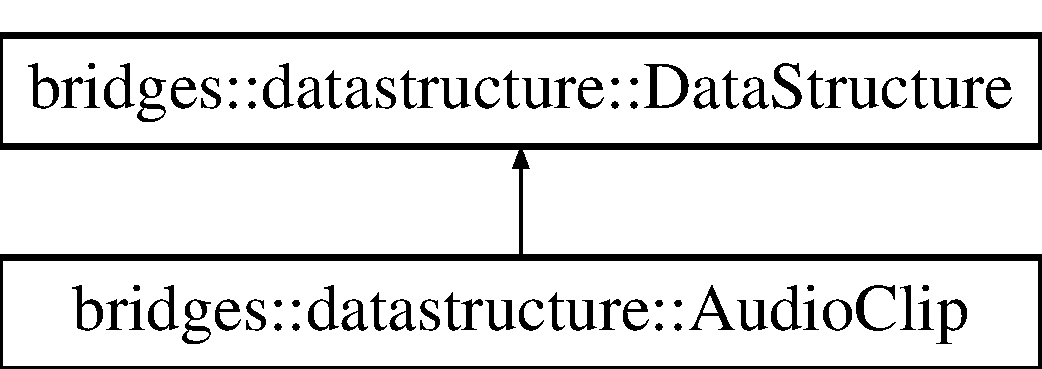
\includegraphics[height=2.000000cm]{classbridges_1_1datastructure_1_1_audio_clip}
\end{center}
\end{figure}
\subsection*{Public Member Functions}
\begin{DoxyCompactItemize}
\item 
\hyperlink{classbridges_1_1datastructure_1_1_audio_clip_aa4db655f2e904a30742d45408ff6543c}{Audio\+Clip} (int sample\+Count, int num\+Channels, int sample\+Bits, int sample\+Rate)
\item 
virtual const string \hyperlink{classbridges_1_1datastructure_1_1_audio_clip_a1fc853180a8d825b2e5ea2d8e3f8e810}{get\+D\+Stype} () const override
\item 
virtual const string \hyperlink{classbridges_1_1datastructure_1_1_audio_clip_a9ff485d7b2e0211d9e5c1432d47be617}{get\+Data\+Structure\+Representation} () const override final
\item 
int \hyperlink{classbridges_1_1datastructure_1_1_audio_clip_a8d685e4e2019e9167d55fc4df3d622d7}{get\+Num\+Channels} ()
\item 
int \hyperlink{classbridges_1_1datastructure_1_1_audio_clip_a1c2df0757e09361c56373debac329a16}{get\+Sample\+Rate} ()
\item 
int \hyperlink{classbridges_1_1datastructure_1_1_audio_clip_a1863f03ae6d0c512c49002108ea78a5d}{get\+Sample\+Count} ()
\item 
int \hyperlink{classbridges_1_1datastructure_1_1_audio_clip_ad8b0a62990aadde10174f077ef0a3441}{get\+Sample\+Bits} ()
\item 
int \hyperlink{classbridges_1_1datastructure_1_1_audio_clip_a2a7fe6f7184a90c5ce781889b3c81307}{get\+Sample} (int channel, int index) const
\item 
void \hyperlink{classbridges_1_1datastructure_1_1_audio_clip_a9f275b8d7cb0a2cf00ec7f8b08e58e8c}{set\+Sample} (int channel, int index, int value)
\end{DoxyCompactItemize}


\subsection{Constructor \& Destructor Documentation}
\mbox{\Hypertarget{classbridges_1_1datastructure_1_1_audio_clip_aa4db655f2e904a30742d45408ff6543c}\label{classbridges_1_1datastructure_1_1_audio_clip_aa4db655f2e904a30742d45408ff6543c}} 
\index{bridges\+::datastructure\+::\+Audio\+Clip@{bridges\+::datastructure\+::\+Audio\+Clip}!Audio\+Clip@{Audio\+Clip}}
\index{Audio\+Clip@{Audio\+Clip}!bridges\+::datastructure\+::\+Audio\+Clip@{bridges\+::datastructure\+::\+Audio\+Clip}}
\subsubsection{\texorpdfstring{Audio\+Clip()}{AudioClip()}}
{\footnotesize\ttfamily bridges\+::datastructure\+::\+Audio\+Clip\+::\+Audio\+Clip (\begin{DoxyParamCaption}\item[{int}]{sample\+Count,  }\item[{int}]{num\+Channels,  }\item[{int}]{sample\+Bits,  }\item[{int}]{sample\+Rate }\end{DoxyParamCaption})\hspace{0.3cm}{\ttfamily [inline]}}



\subsection{Member Function Documentation}
\mbox{\Hypertarget{classbridges_1_1datastructure_1_1_audio_clip_a9ff485d7b2e0211d9e5c1432d47be617}\label{classbridges_1_1datastructure_1_1_audio_clip_a9ff485d7b2e0211d9e5c1432d47be617}} 
\index{bridges\+::datastructure\+::\+Audio\+Clip@{bridges\+::datastructure\+::\+Audio\+Clip}!get\+Data\+Structure\+Representation@{get\+Data\+Structure\+Representation}}
\index{get\+Data\+Structure\+Representation@{get\+Data\+Structure\+Representation}!bridges\+::datastructure\+::\+Audio\+Clip@{bridges\+::datastructure\+::\+Audio\+Clip}}
\subsubsection{\texorpdfstring{get\+Data\+Structure\+Representation()}{getDataStructureRepresentation()}}
{\footnotesize\ttfamily virtual const string bridges\+::datastructure\+::\+Audio\+Clip\+::get\+Data\+Structure\+Representation (\begin{DoxyParamCaption}{ }\end{DoxyParamCaption}) const\hspace{0.3cm}{\ttfamily [inline]}, {\ttfamily [final]}, {\ttfamily [override]}, {\ttfamily [virtual]}}

Ease of use function for the deletion of an entire datastructure. Overrides should call delete on itself and each linked data structure

\begin{DoxyWarning}{Warning}
Only call if all these data structures were all dynamicaly allocated(aka\+: using new) Gets the J\+S\+ON representation of this \hyperlink{classbridges_1_1datastructure_1_1_data_structure}{Data\+Structure}\textquotesingle{}s nodes and links
\end{DoxyWarning}
\begin{DoxyReturn}{Returns}
The J\+S\+ON representation of the data structure\+: A pair holding the nodes and links J\+S\+ON strings respectively 
\end{DoxyReturn}


Implements \hyperlink{classbridges_1_1datastructure_1_1_data_structure}{bridges\+::datastructure\+::\+Data\+Structure}.

\mbox{\Hypertarget{classbridges_1_1datastructure_1_1_audio_clip_a1fc853180a8d825b2e5ea2d8e3f8e810}\label{classbridges_1_1datastructure_1_1_audio_clip_a1fc853180a8d825b2e5ea2d8e3f8e810}} 
\index{bridges\+::datastructure\+::\+Audio\+Clip@{bridges\+::datastructure\+::\+Audio\+Clip}!get\+D\+Stype@{get\+D\+Stype}}
\index{get\+D\+Stype@{get\+D\+Stype}!bridges\+::datastructure\+::\+Audio\+Clip@{bridges\+::datastructure\+::\+Audio\+Clip}}
\subsubsection{\texorpdfstring{get\+D\+Stype()}{getDStype()}}
{\footnotesize\ttfamily virtual const string bridges\+::datastructure\+::\+Audio\+Clip\+::get\+D\+Stype (\begin{DoxyParamCaption}{ }\end{DoxyParamCaption}) const\hspace{0.3cm}{\ttfamily [inline]}, {\ttfamily [override]}, {\ttfamily [virtual]}}

\begin{DoxyReturn}{Returns}
The string representation of this data structure type 
\end{DoxyReturn}


Implements \hyperlink{classbridges_1_1datastructure_1_1_data_structure_a4ff66cb34409f11fe9fc647f6d8a22ce}{bridges\+::datastructure\+::\+Data\+Structure}.

\mbox{\Hypertarget{classbridges_1_1datastructure_1_1_audio_clip_a8d685e4e2019e9167d55fc4df3d622d7}\label{classbridges_1_1datastructure_1_1_audio_clip_a8d685e4e2019e9167d55fc4df3d622d7}} 
\index{bridges\+::datastructure\+::\+Audio\+Clip@{bridges\+::datastructure\+::\+Audio\+Clip}!get\+Num\+Channels@{get\+Num\+Channels}}
\index{get\+Num\+Channels@{get\+Num\+Channels}!bridges\+::datastructure\+::\+Audio\+Clip@{bridges\+::datastructure\+::\+Audio\+Clip}}
\subsubsection{\texorpdfstring{get\+Num\+Channels()}{getNumChannels()}}
{\footnotesize\ttfamily int bridges\+::datastructure\+::\+Audio\+Clip\+::get\+Num\+Channels (\begin{DoxyParamCaption}{ }\end{DoxyParamCaption})\hspace{0.3cm}{\ttfamily [inline]}}

\mbox{\Hypertarget{classbridges_1_1datastructure_1_1_audio_clip_a2a7fe6f7184a90c5ce781889b3c81307}\label{classbridges_1_1datastructure_1_1_audio_clip_a2a7fe6f7184a90c5ce781889b3c81307}} 
\index{bridges\+::datastructure\+::\+Audio\+Clip@{bridges\+::datastructure\+::\+Audio\+Clip}!get\+Sample@{get\+Sample}}
\index{get\+Sample@{get\+Sample}!bridges\+::datastructure\+::\+Audio\+Clip@{bridges\+::datastructure\+::\+Audio\+Clip}}
\subsubsection{\texorpdfstring{get\+Sample()}{getSample()}}
{\footnotesize\ttfamily int bridges\+::datastructure\+::\+Audio\+Clip\+::get\+Sample (\begin{DoxyParamCaption}\item[{int}]{channel,  }\item[{int}]{index }\end{DoxyParamCaption}) const\hspace{0.3cm}{\ttfamily [inline]}}

\mbox{\Hypertarget{classbridges_1_1datastructure_1_1_audio_clip_ad8b0a62990aadde10174f077ef0a3441}\label{classbridges_1_1datastructure_1_1_audio_clip_ad8b0a62990aadde10174f077ef0a3441}} 
\index{bridges\+::datastructure\+::\+Audio\+Clip@{bridges\+::datastructure\+::\+Audio\+Clip}!get\+Sample\+Bits@{get\+Sample\+Bits}}
\index{get\+Sample\+Bits@{get\+Sample\+Bits}!bridges\+::datastructure\+::\+Audio\+Clip@{bridges\+::datastructure\+::\+Audio\+Clip}}
\subsubsection{\texorpdfstring{get\+Sample\+Bits()}{getSampleBits()}}
{\footnotesize\ttfamily int bridges\+::datastructure\+::\+Audio\+Clip\+::get\+Sample\+Bits (\begin{DoxyParamCaption}{ }\end{DoxyParamCaption})\hspace{0.3cm}{\ttfamily [inline]}}

\mbox{\Hypertarget{classbridges_1_1datastructure_1_1_audio_clip_a1863f03ae6d0c512c49002108ea78a5d}\label{classbridges_1_1datastructure_1_1_audio_clip_a1863f03ae6d0c512c49002108ea78a5d}} 
\index{bridges\+::datastructure\+::\+Audio\+Clip@{bridges\+::datastructure\+::\+Audio\+Clip}!get\+Sample\+Count@{get\+Sample\+Count}}
\index{get\+Sample\+Count@{get\+Sample\+Count}!bridges\+::datastructure\+::\+Audio\+Clip@{bridges\+::datastructure\+::\+Audio\+Clip}}
\subsubsection{\texorpdfstring{get\+Sample\+Count()}{getSampleCount()}}
{\footnotesize\ttfamily int bridges\+::datastructure\+::\+Audio\+Clip\+::get\+Sample\+Count (\begin{DoxyParamCaption}{ }\end{DoxyParamCaption})\hspace{0.3cm}{\ttfamily [inline]}}

\mbox{\Hypertarget{classbridges_1_1datastructure_1_1_audio_clip_a1c2df0757e09361c56373debac329a16}\label{classbridges_1_1datastructure_1_1_audio_clip_a1c2df0757e09361c56373debac329a16}} 
\index{bridges\+::datastructure\+::\+Audio\+Clip@{bridges\+::datastructure\+::\+Audio\+Clip}!get\+Sample\+Rate@{get\+Sample\+Rate}}
\index{get\+Sample\+Rate@{get\+Sample\+Rate}!bridges\+::datastructure\+::\+Audio\+Clip@{bridges\+::datastructure\+::\+Audio\+Clip}}
\subsubsection{\texorpdfstring{get\+Sample\+Rate()}{getSampleRate()}}
{\footnotesize\ttfamily int bridges\+::datastructure\+::\+Audio\+Clip\+::get\+Sample\+Rate (\begin{DoxyParamCaption}{ }\end{DoxyParamCaption})\hspace{0.3cm}{\ttfamily [inline]}}

\mbox{\Hypertarget{classbridges_1_1datastructure_1_1_audio_clip_a9f275b8d7cb0a2cf00ec7f8b08e58e8c}\label{classbridges_1_1datastructure_1_1_audio_clip_a9f275b8d7cb0a2cf00ec7f8b08e58e8c}} 
\index{bridges\+::datastructure\+::\+Audio\+Clip@{bridges\+::datastructure\+::\+Audio\+Clip}!set\+Sample@{set\+Sample}}
\index{set\+Sample@{set\+Sample}!bridges\+::datastructure\+::\+Audio\+Clip@{bridges\+::datastructure\+::\+Audio\+Clip}}
\subsubsection{\texorpdfstring{set\+Sample()}{setSample()}}
{\footnotesize\ttfamily void bridges\+::datastructure\+::\+Audio\+Clip\+::set\+Sample (\begin{DoxyParamCaption}\item[{int}]{channel,  }\item[{int}]{index,  }\item[{int}]{value }\end{DoxyParamCaption})\hspace{0.3cm}{\ttfamily [inline]}}



The documentation for this class was generated from the following file\+:\begin{DoxyCompactItemize}
\item 
/home/erik/work/bridges/bridges-\/cxx/src/\hyperlink{_audio_clip_8h}{Audio\+Clip.\+h}\end{DoxyCompactItemize}

\hypertarget{classbridges_1_1datastructure_1_1_a_v_l_tree_element}{}\section{bridges\+::datastructure\+::A\+V\+L\+Tree\+Element$<$ K, E $>$ Class Template Reference}
\label{classbridges_1_1datastructure_1_1_a_v_l_tree_element}\index{bridges::datastructure::AVLTreeElement$<$ K, E $>$@{bridges::datastructure::AVLTreeElement$<$ K, E $>$}}


{\ttfamily \#include $<$A\+V\+L\+Tree\+Element.\+h$>$}

Inheritance diagram for bridges\+::datastructure\+::A\+V\+L\+Tree\+Element$<$ K, E $>$\+:\begin{figure}[H]
\begin{center}
\leavevmode
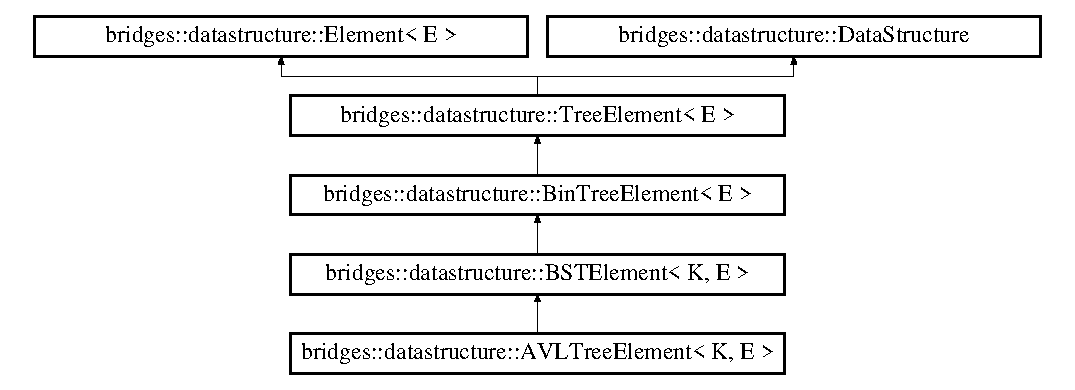
\includegraphics[height=4.794520cm]{classbridges_1_1datastructure_1_1_a_v_l_tree_element}
\end{center}
\end{figure}


\subsection{Detailed Description}
\subsubsection*{template$<$typename K, typename E$>$\newline
class bridges\+::datastructure\+::\+A\+V\+L\+Tree\+Element$<$ K, E $>$}

This class can be used to create avl tree elements, derived from \mbox{\hyperlink{classbridges_1_1datastructure_1_1_b_s_t_element}{B\+S\+T\+Element}}. 

This class extends the \mbox{\hyperlink{classbridges_1_1datastructure_1_1_b_s_t_element}{B\+S\+T\+Element}} class by adding height and balance factor attributes to allow for easier use in a avl tree implementation.

Generic Parameters\+: K that is the search key type, E the application data type

\begin{DoxyAuthor}{Author}
Kalpathi Subramanian 
\end{DoxyAuthor}
\begin{DoxyDate}{Date}
6/18/15, 7/15/16
\end{DoxyDate}
There is a tutorial about A\+V\+Ls \+: \href{http://bridgesuncc.github.io/tutorials/AVL.html}{\texttt{ http\+://bridgesuncc.\+github.\+io/tutorials/\+A\+V\+L.\+html}} \subsection*{Public Member Functions}
\begin{DoxyCompactItemize}
\item 
\mbox{\hyperlink{classbridges_1_1datastructure_1_1_a_v_l_tree_element_a611fc818eeb478e330ef585adcefd9e6}{A\+V\+L\+Tree\+Element}} (const K \&k, const E \&val=E(), const string \&lab=string())
\item 
virtual const string \mbox{\hyperlink{classbridges_1_1datastructure_1_1_a_v_l_tree_element_ab04d1e9ad4630e408041e8137dc9854a}{get\+D\+Stype}} () const override
\item 
int \mbox{\hyperlink{classbridges_1_1datastructure_1_1_a_v_l_tree_element_a5d4b990d49f6f3d2f23f4dd3e57414e8}{get\+Height}} () const
\item 
void \mbox{\hyperlink{classbridges_1_1datastructure_1_1_a_v_l_tree_element_af387bcd2b37b7284ea983acafecff93c}{set\+Height}} (const int \&h)
\item 
int \mbox{\hyperlink{classbridges_1_1datastructure_1_1_a_v_l_tree_element_ade3c059448d00ac50dac89e59864b11f}{get\+Balance\+Factor}} () const
\item 
void \mbox{\hyperlink{classbridges_1_1datastructure_1_1_a_v_l_tree_element_a32af51a86585479c28de425374df95e9}{set\+Balance\+Factor}} (const int \&bf)
\item 
virtual \mbox{\hyperlink{classbridges_1_1datastructure_1_1_a_v_l_tree_element}{A\+V\+L\+Tree\+Element}} $\ast$ \mbox{\hyperlink{classbridges_1_1datastructure_1_1_a_v_l_tree_element_ab05925e343b9fa71b61c71e8034e1293}{get\+Left}} () override
\item 
virtual const \mbox{\hyperlink{classbridges_1_1datastructure_1_1_a_v_l_tree_element}{A\+V\+L\+Tree\+Element}} $\ast$ \mbox{\hyperlink{classbridges_1_1datastructure_1_1_a_v_l_tree_element_a4a639e0c623435aadf5c51ed132cb25d}{get\+Left}} () const override
\item 
void \mbox{\hyperlink{classbridges_1_1datastructure_1_1_a_v_l_tree_element_af6c8a71789ff45481786fd4d63cbbcbe}{set\+Left}} (\mbox{\hyperlink{classbridges_1_1datastructure_1_1_a_v_l_tree_element}{A\+V\+L\+Tree\+Element}} $\ast$l)
\item 
virtual \mbox{\hyperlink{classbridges_1_1datastructure_1_1_a_v_l_tree_element}{A\+V\+L\+Tree\+Element}} $\ast$ \mbox{\hyperlink{classbridges_1_1datastructure_1_1_a_v_l_tree_element_aed585fdf56fcbfebac6cd0262c9c1807}{get\+Right}} () override
\item 
virtual const \mbox{\hyperlink{classbridges_1_1datastructure_1_1_a_v_l_tree_element}{A\+V\+L\+Tree\+Element}} $\ast$ \mbox{\hyperlink{classbridges_1_1datastructure_1_1_a_v_l_tree_element_a5a2c4b96b51da1daa3c0426882250acb}{get\+Right}} () const override
\item 
void \mbox{\hyperlink{classbridges_1_1datastructure_1_1_a_v_l_tree_element_a8ef25fb87bcce418541adccb17cbee80}{set\+Right}} (\mbox{\hyperlink{classbridges_1_1datastructure_1_1_a_v_l_tree_element}{A\+V\+L\+Tree\+Element}} $\ast$r)
\end{DoxyCompactItemize}
\subsection*{Additional Inherited Members}


\subsection{Constructor \& Destructor Documentation}
\mbox{\Hypertarget{classbridges_1_1datastructure_1_1_a_v_l_tree_element_a611fc818eeb478e330ef585adcefd9e6}\label{classbridges_1_1datastructure_1_1_a_v_l_tree_element_a611fc818eeb478e330ef585adcefd9e6}} 
\index{bridges::datastructure::AVLTreeElement$<$ K, E $>$@{bridges::datastructure::AVLTreeElement$<$ K, E $>$}!AVLTreeElement@{AVLTreeElement}}
\index{AVLTreeElement@{AVLTreeElement}!bridges::datastructure::AVLTreeElement$<$ K, E $>$@{bridges::datastructure::AVLTreeElement$<$ K, E $>$}}
\subsubsection{\texorpdfstring{AVLTreeElement()}{AVLTreeElement()}}
{\footnotesize\ttfamily template$<$typename K , typename E $>$ \\
\mbox{\hyperlink{classbridges_1_1datastructure_1_1_a_v_l_tree_element}{bridges\+::datastructure\+::\+A\+V\+L\+Tree\+Element}}$<$ K, E $>$\+::\mbox{\hyperlink{classbridges_1_1datastructure_1_1_a_v_l_tree_element}{A\+V\+L\+Tree\+Element}} (\begin{DoxyParamCaption}\item[{const K \&}]{k,  }\item[{const E \&}]{val = {\ttfamily E()},  }\item[{const string \&}]{lab = {\ttfamily string()} }\end{DoxyParamCaption})\hspace{0.3cm}{\ttfamily [inline]}}

Constructs a \mbox{\hyperlink{classbridges_1_1datastructure_1_1_a_v_l_tree_element}{A\+V\+L\+Tree\+Element}} with the provided value, label, key, setting the left and right A\+V\+L\+Tree\+Elements to N\+U\+LL. The defaults will be used if not provided.


\begin{DoxyParams}{Parameters}
{\em k} & The key for ordering \\
\hline
{\em val} & The data to hold \\
\hline
{\em lab} & The label to show \\
\hline
\end{DoxyParams}


\subsection{Member Function Documentation}
\mbox{\Hypertarget{classbridges_1_1datastructure_1_1_a_v_l_tree_element_ade3c059448d00ac50dac89e59864b11f}\label{classbridges_1_1datastructure_1_1_a_v_l_tree_element_ade3c059448d00ac50dac89e59864b11f}} 
\index{bridges::datastructure::AVLTreeElement$<$ K, E $>$@{bridges::datastructure::AVLTreeElement$<$ K, E $>$}!getBalanceFactor@{getBalanceFactor}}
\index{getBalanceFactor@{getBalanceFactor}!bridges::datastructure::AVLTreeElement$<$ K, E $>$@{bridges::datastructure::AVLTreeElement$<$ K, E $>$}}
\subsubsection{\texorpdfstring{getBalanceFactor()}{getBalanceFactor()}}
{\footnotesize\ttfamily template$<$typename K , typename E $>$ \\
int \mbox{\hyperlink{classbridges_1_1datastructure_1_1_a_v_l_tree_element}{bridges\+::datastructure\+::\+A\+V\+L\+Tree\+Element}}$<$ K, E $>$\+::get\+Balance\+Factor (\begin{DoxyParamCaption}{ }\end{DoxyParamCaption}) const\hspace{0.3cm}{\ttfamily [inline]}}

Get balance factor of this node \begin{DoxyReturn}{Returns}
The balance factor of this \mbox{\hyperlink{classbridges_1_1datastructure_1_1_a_v_l_tree_element}{A\+V\+L\+Tree\+Element}} 
\end{DoxyReturn}
\mbox{\Hypertarget{classbridges_1_1datastructure_1_1_a_v_l_tree_element_ab04d1e9ad4630e408041e8137dc9854a}\label{classbridges_1_1datastructure_1_1_a_v_l_tree_element_ab04d1e9ad4630e408041e8137dc9854a}} 
\index{bridges::datastructure::AVLTreeElement$<$ K, E $>$@{bridges::datastructure::AVLTreeElement$<$ K, E $>$}!getDStype@{getDStype}}
\index{getDStype@{getDStype}!bridges::datastructure::AVLTreeElement$<$ K, E $>$@{bridges::datastructure::AVLTreeElement$<$ K, E $>$}}
\subsubsection{\texorpdfstring{getDStype()}{getDStype()}}
{\footnotesize\ttfamily template$<$typename K , typename E $>$ \\
virtual const string \mbox{\hyperlink{classbridges_1_1datastructure_1_1_a_v_l_tree_element}{bridges\+::datastructure\+::\+A\+V\+L\+Tree\+Element}}$<$ K, E $>$\+::get\+D\+Stype (\begin{DoxyParamCaption}{ }\end{DoxyParamCaption}) const\hspace{0.3cm}{\ttfamily [inline]}, {\ttfamily [override]}, {\ttfamily [virtual]}}

Return the data structure name \begin{DoxyReturn}{Returns}
the data structure type 
\end{DoxyReturn}


Reimplemented from \mbox{\hyperlink{classbridges_1_1datastructure_1_1_b_s_t_element_a2bb8cc9ec4b6bc5b89ecef0f17be366f}{bridges\+::datastructure\+::\+B\+S\+T\+Element$<$ K, E $>$}}.

\mbox{\Hypertarget{classbridges_1_1datastructure_1_1_a_v_l_tree_element_a5d4b990d49f6f3d2f23f4dd3e57414e8}\label{classbridges_1_1datastructure_1_1_a_v_l_tree_element_a5d4b990d49f6f3d2f23f4dd3e57414e8}} 
\index{bridges::datastructure::AVLTreeElement$<$ K, E $>$@{bridges::datastructure::AVLTreeElement$<$ K, E $>$}!getHeight@{getHeight}}
\index{getHeight@{getHeight}!bridges::datastructure::AVLTreeElement$<$ K, E $>$@{bridges::datastructure::AVLTreeElement$<$ K, E $>$}}
\subsubsection{\texorpdfstring{getHeight()}{getHeight()}}
{\footnotesize\ttfamily template$<$typename K , typename E $>$ \\
int \mbox{\hyperlink{classbridges_1_1datastructure_1_1_a_v_l_tree_element}{bridges\+::datastructure\+::\+A\+V\+L\+Tree\+Element}}$<$ K, E $>$\+::get\+Height (\begin{DoxyParamCaption}{ }\end{DoxyParamCaption}) const\hspace{0.3cm}{\ttfamily [inline]}}

Get the height of the tree \begin{DoxyReturn}{Returns}
The height of this \mbox{\hyperlink{classbridges_1_1datastructure_1_1_a_v_l_tree_element}{A\+V\+L\+Tree\+Element}} 
\end{DoxyReturn}
\mbox{\Hypertarget{classbridges_1_1datastructure_1_1_a_v_l_tree_element_ab05925e343b9fa71b61c71e8034e1293}\label{classbridges_1_1datastructure_1_1_a_v_l_tree_element_ab05925e343b9fa71b61c71e8034e1293}} 
\index{bridges::datastructure::AVLTreeElement$<$ K, E $>$@{bridges::datastructure::AVLTreeElement$<$ K, E $>$}!getLeft@{getLeft}}
\index{getLeft@{getLeft}!bridges::datastructure::AVLTreeElement$<$ K, E $>$@{bridges::datastructure::AVLTreeElement$<$ K, E $>$}}
\subsubsection{\texorpdfstring{getLeft()}{getLeft()}\hspace{0.1cm}{\footnotesize\ttfamily [1/2]}}
{\footnotesize\ttfamily template$<$typename K , typename E $>$ \\
virtual \mbox{\hyperlink{classbridges_1_1datastructure_1_1_a_v_l_tree_element}{A\+V\+L\+Tree\+Element}}$\ast$ \mbox{\hyperlink{classbridges_1_1datastructure_1_1_a_v_l_tree_element}{bridges\+::datastructure\+::\+A\+V\+L\+Tree\+Element}}$<$ K, E $>$\+::get\+Left (\begin{DoxyParamCaption}{ }\end{DoxyParamCaption})\hspace{0.3cm}{\ttfamily [inline]}, {\ttfamily [override]}, {\ttfamily [virtual]}}

Gets the left child \begin{DoxyReturn}{Returns}
The left child 
\end{DoxyReturn}


Reimplemented from \mbox{\hyperlink{classbridges_1_1datastructure_1_1_b_s_t_element_af863c624691c11db26ae3b6d723d1f5c}{bridges\+::datastructure\+::\+B\+S\+T\+Element$<$ K, E $>$}}.

\mbox{\Hypertarget{classbridges_1_1datastructure_1_1_a_v_l_tree_element_a4a639e0c623435aadf5c51ed132cb25d}\label{classbridges_1_1datastructure_1_1_a_v_l_tree_element_a4a639e0c623435aadf5c51ed132cb25d}} 
\index{bridges::datastructure::AVLTreeElement$<$ K, E $>$@{bridges::datastructure::AVLTreeElement$<$ K, E $>$}!getLeft@{getLeft}}
\index{getLeft@{getLeft}!bridges::datastructure::AVLTreeElement$<$ K, E $>$@{bridges::datastructure::AVLTreeElement$<$ K, E $>$}}
\subsubsection{\texorpdfstring{getLeft()}{getLeft()}\hspace{0.1cm}{\footnotesize\ttfamily [2/2]}}
{\footnotesize\ttfamily template$<$typename K , typename E $>$ \\
virtual const \mbox{\hyperlink{classbridges_1_1datastructure_1_1_a_v_l_tree_element}{A\+V\+L\+Tree\+Element}}$\ast$ \mbox{\hyperlink{classbridges_1_1datastructure_1_1_a_v_l_tree_element}{bridges\+::datastructure\+::\+A\+V\+L\+Tree\+Element}}$<$ K, E $>$\+::get\+Left (\begin{DoxyParamCaption}{ }\end{DoxyParamCaption}) const\hspace{0.3cm}{\ttfamily [inline]}, {\ttfamily [override]}, {\ttfamily [virtual]}}

Gets the left child -\/ Constant version

\begin{DoxyReturn}{Returns}
The left child 
\end{DoxyReturn}


Reimplemented from \mbox{\hyperlink{classbridges_1_1datastructure_1_1_b_s_t_element_abac324ef0b480420bd82ecfe4501d60d}{bridges\+::datastructure\+::\+B\+S\+T\+Element$<$ K, E $>$}}.

\mbox{\Hypertarget{classbridges_1_1datastructure_1_1_a_v_l_tree_element_aed585fdf56fcbfebac6cd0262c9c1807}\label{classbridges_1_1datastructure_1_1_a_v_l_tree_element_aed585fdf56fcbfebac6cd0262c9c1807}} 
\index{bridges::datastructure::AVLTreeElement$<$ K, E $>$@{bridges::datastructure::AVLTreeElement$<$ K, E $>$}!getRight@{getRight}}
\index{getRight@{getRight}!bridges::datastructure::AVLTreeElement$<$ K, E $>$@{bridges::datastructure::AVLTreeElement$<$ K, E $>$}}
\subsubsection{\texorpdfstring{getRight()}{getRight()}\hspace{0.1cm}{\footnotesize\ttfamily [1/2]}}
{\footnotesize\ttfamily template$<$typename K , typename E $>$ \\
virtual \mbox{\hyperlink{classbridges_1_1datastructure_1_1_a_v_l_tree_element}{A\+V\+L\+Tree\+Element}}$\ast$ \mbox{\hyperlink{classbridges_1_1datastructure_1_1_a_v_l_tree_element}{bridges\+::datastructure\+::\+A\+V\+L\+Tree\+Element}}$<$ K, E $>$\+::get\+Right (\begin{DoxyParamCaption}{ }\end{DoxyParamCaption})\hspace{0.3cm}{\ttfamily [inline]}, {\ttfamily [override]}, {\ttfamily [virtual]}}

Return the right child \begin{DoxyReturn}{Returns}
The right child 
\end{DoxyReturn}


Reimplemented from \mbox{\hyperlink{classbridges_1_1datastructure_1_1_b_s_t_element_a80f5085d6d03805dd3091b7693d8e235}{bridges\+::datastructure\+::\+B\+S\+T\+Element$<$ K, E $>$}}.

\mbox{\Hypertarget{classbridges_1_1datastructure_1_1_a_v_l_tree_element_a5a2c4b96b51da1daa3c0426882250acb}\label{classbridges_1_1datastructure_1_1_a_v_l_tree_element_a5a2c4b96b51da1daa3c0426882250acb}} 
\index{bridges::datastructure::AVLTreeElement$<$ K, E $>$@{bridges::datastructure::AVLTreeElement$<$ K, E $>$}!getRight@{getRight}}
\index{getRight@{getRight}!bridges::datastructure::AVLTreeElement$<$ K, E $>$@{bridges::datastructure::AVLTreeElement$<$ K, E $>$}}
\subsubsection{\texorpdfstring{getRight()}{getRight()}\hspace{0.1cm}{\footnotesize\ttfamily [2/2]}}
{\footnotesize\ttfamily template$<$typename K , typename E $>$ \\
virtual const \mbox{\hyperlink{classbridges_1_1datastructure_1_1_a_v_l_tree_element}{A\+V\+L\+Tree\+Element}}$\ast$ \mbox{\hyperlink{classbridges_1_1datastructure_1_1_a_v_l_tree_element}{bridges\+::datastructure\+::\+A\+V\+L\+Tree\+Element}}$<$ K, E $>$\+::get\+Right (\begin{DoxyParamCaption}{ }\end{DoxyParamCaption}) const\hspace{0.3cm}{\ttfamily [inline]}, {\ttfamily [override]}, {\ttfamily [virtual]}}

Return the right child -\/ Constant version

\begin{DoxyReturn}{Returns}
The right child 
\end{DoxyReturn}


Reimplemented from \mbox{\hyperlink{classbridges_1_1datastructure_1_1_b_s_t_element_a012f0eb09c3d62b14c73109e6ded0879}{bridges\+::datastructure\+::\+B\+S\+T\+Element$<$ K, E $>$}}.

\mbox{\Hypertarget{classbridges_1_1datastructure_1_1_a_v_l_tree_element_a32af51a86585479c28de425374df95e9}\label{classbridges_1_1datastructure_1_1_a_v_l_tree_element_a32af51a86585479c28de425374df95e9}} 
\index{bridges::datastructure::AVLTreeElement$<$ K, E $>$@{bridges::datastructure::AVLTreeElement$<$ K, E $>$}!setBalanceFactor@{setBalanceFactor}}
\index{setBalanceFactor@{setBalanceFactor}!bridges::datastructure::AVLTreeElement$<$ K, E $>$@{bridges::datastructure::AVLTreeElement$<$ K, E $>$}}
\subsubsection{\texorpdfstring{setBalanceFactor()}{setBalanceFactor()}}
{\footnotesize\ttfamily template$<$typename K , typename E $>$ \\
void \mbox{\hyperlink{classbridges_1_1datastructure_1_1_a_v_l_tree_element}{bridges\+::datastructure\+::\+A\+V\+L\+Tree\+Element}}$<$ K, E $>$\+::set\+Balance\+Factor (\begin{DoxyParamCaption}\item[{const int \&}]{bf }\end{DoxyParamCaption})\hspace{0.3cm}{\ttfamily [inline]}}

Set the balance factor to \char`\"{}bf\char`\"{}
\begin{DoxyParams}{Parameters}
{\em bf} & The balance factor of this \mbox{\hyperlink{classbridges_1_1datastructure_1_1_a_v_l_tree_element}{A\+V\+L\+Tree\+Element}}\\
\hline
{\em bf} & the balance factor to set at this node \\
\hline
\end{DoxyParams}
\mbox{\Hypertarget{classbridges_1_1datastructure_1_1_a_v_l_tree_element_af387bcd2b37b7284ea983acafecff93c}\label{classbridges_1_1datastructure_1_1_a_v_l_tree_element_af387bcd2b37b7284ea983acafecff93c}} 
\index{bridges::datastructure::AVLTreeElement$<$ K, E $>$@{bridges::datastructure::AVLTreeElement$<$ K, E $>$}!setHeight@{setHeight}}
\index{setHeight@{setHeight}!bridges::datastructure::AVLTreeElement$<$ K, E $>$@{bridges::datastructure::AVLTreeElement$<$ K, E $>$}}
\subsubsection{\texorpdfstring{setHeight()}{setHeight()}}
{\footnotesize\ttfamily template$<$typename K , typename E $>$ \\
void \mbox{\hyperlink{classbridges_1_1datastructure_1_1_a_v_l_tree_element}{bridges\+::datastructure\+::\+A\+V\+L\+Tree\+Element}}$<$ K, E $>$\+::set\+Height (\begin{DoxyParamCaption}\item[{const int \&}]{h }\end{DoxyParamCaption})\hspace{0.3cm}{\ttfamily [inline]}}

Set the height to \char`\"{}h\char`\"{}


\begin{DoxyParams}{Parameters}
{\em h} & the height of the tree at this node \\
\hline
\end{DoxyParams}
\mbox{\Hypertarget{classbridges_1_1datastructure_1_1_a_v_l_tree_element_af6c8a71789ff45481786fd4d63cbbcbe}\label{classbridges_1_1datastructure_1_1_a_v_l_tree_element_af6c8a71789ff45481786fd4d63cbbcbe}} 
\index{bridges::datastructure::AVLTreeElement$<$ K, E $>$@{bridges::datastructure::AVLTreeElement$<$ K, E $>$}!setLeft@{setLeft}}
\index{setLeft@{setLeft}!bridges::datastructure::AVLTreeElement$<$ K, E $>$@{bridges::datastructure::AVLTreeElement$<$ K, E $>$}}
\subsubsection{\texorpdfstring{setLeft()}{setLeft()}}
{\footnotesize\ttfamily template$<$typename K , typename E $>$ \\
void \mbox{\hyperlink{classbridges_1_1datastructure_1_1_a_v_l_tree_element}{bridges\+::datastructure\+::\+A\+V\+L\+Tree\+Element}}$<$ K, E $>$\+::set\+Left (\begin{DoxyParamCaption}\item[{\mbox{\hyperlink{classbridges_1_1datastructure_1_1_a_v_l_tree_element}{A\+V\+L\+Tree\+Element}}$<$ K, E $>$ $\ast$}]{l }\end{DoxyParamCaption})\hspace{0.3cm}{\ttfamily [inline]}}

Sets left child to \char`\"{}l\char`\"{}


\begin{DoxyParams}{Parameters}
{\em l} & The left tree element \\
\hline
\end{DoxyParams}
\mbox{\Hypertarget{classbridges_1_1datastructure_1_1_a_v_l_tree_element_a8ef25fb87bcce418541adccb17cbee80}\label{classbridges_1_1datastructure_1_1_a_v_l_tree_element_a8ef25fb87bcce418541adccb17cbee80}} 
\index{bridges::datastructure::AVLTreeElement$<$ K, E $>$@{bridges::datastructure::AVLTreeElement$<$ K, E $>$}!setRight@{setRight}}
\index{setRight@{setRight}!bridges::datastructure::AVLTreeElement$<$ K, E $>$@{bridges::datastructure::AVLTreeElement$<$ K, E $>$}}
\subsubsection{\texorpdfstring{setRight()}{setRight()}}
{\footnotesize\ttfamily template$<$typename K , typename E $>$ \\
void \mbox{\hyperlink{classbridges_1_1datastructure_1_1_a_v_l_tree_element}{bridges\+::datastructure\+::\+A\+V\+L\+Tree\+Element}}$<$ K, E $>$\+::set\+Right (\begin{DoxyParamCaption}\item[{\mbox{\hyperlink{classbridges_1_1datastructure_1_1_a_v_l_tree_element}{A\+V\+L\+Tree\+Element}}$<$ K, E $>$ $\ast$}]{r }\end{DoxyParamCaption})\hspace{0.3cm}{\ttfamily [inline]}}

Sets right child to \char`\"{}r\char`\"{}


\begin{DoxyParams}{Parameters}
{\em r} & The right \mbox{\hyperlink{classbridges_1_1datastructure_1_1_b_s_t_element}{B\+S\+T\+Element}} \\
\hline
\end{DoxyParams}


The documentation for this class was generated from the following file\+:\begin{DoxyCompactItemize}
\item 
/\+Users/kalpathi/gr/bridges/cxx/src/\mbox{\hyperlink{_a_v_l_tree_element_8h}{A\+V\+L\+Tree\+Element.\+h}}\end{DoxyCompactItemize}

\hypertarget{classbridges_1_1benchmark_1_1_b_f_s_benchmark}{}\section{bridges\+::benchmark\+::B\+F\+S\+Benchmark Class Reference}
\label{classbridges_1_1benchmark_1_1_b_f_s_benchmark}\index{bridges::benchmark::BFSBenchmark@{bridges::benchmark::BFSBenchmark}}


{\ttfamily \#include $<$B\+F\+S\+Benchmark.\+h$>$}

Inheritance diagram for bridges\+::benchmark\+::B\+F\+S\+Benchmark\+:\begin{figure}[H]
\begin{center}
\leavevmode
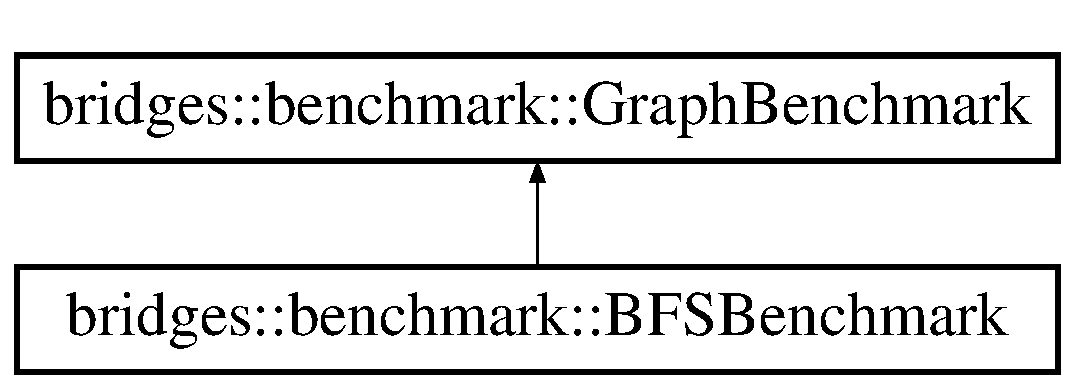
\includegraphics[height=2.000000cm]{classbridges_1_1benchmark_1_1_b_f_s_benchmark}
\end{center}
\end{figure}


\subsection{Detailed Description}
Benchmarks Breadth First Search algorithms. 

Benchmarks B\+FS algorithms and add time series to a Line\+Chart.

One can also set a maximum time spent on a particular run using \mbox{\hyperlink{classbridges_1_1benchmark_1_1_graph_benchmark_a56934eb2789e54c088e7b4423c3a7456}{set\+Time\+Cap()}}.

The B\+FS algorithms must have for prototype\+:

void ($\ast$bfsalgo)(const Graph\+Adj\+List$<$std\+::string$>$\& gr, std\+::string root, std\+::unordered\+\_\+map$<$std\+::string, int$>$\& level, std\+::unordered\+\_\+map$<$std\+::string, std\+::string$>$\& parent);

and can be passed to the run function for being benchmarked. A typical use would look something like


\begin{DoxyCode}{0}
\DoxyCodeLine{LineChart lc;}
\DoxyCodeLine{\mbox{\hyperlink{classbridges_1_1benchmark_1_1_b_f_s_benchmark_abd3525c2c0512a397c29ca41ae6982df}{BFSBenchmark}} sb (lc);}
\DoxyCodeLine{sb.run(\textcolor{stringliteral}{"mybfsalgorithm"}, bfsalgo);}
\end{DoxyCode}


\begin{DoxyAuthor}{Author}
Erik Saule 
\end{DoxyAuthor}
\begin{DoxyDate}{Date}
07/21/2019 
\end{DoxyDate}
\subsection*{Public Member Functions}
\begin{DoxyCompactItemize}
\item 
\mbox{\hyperlink{classbridges_1_1benchmark_1_1_b_f_s_benchmark_abd3525c2c0512a397c29ca41ae6982df}{B\+F\+S\+Benchmark}} (\mbox{\hyperlink{classbridges_1_1datastructure_1_1_line_chart}{Line\+Chart}} \&p)
\item 
void \mbox{\hyperlink{classbridges_1_1benchmark_1_1_b_f_s_benchmark_a8ac66a16c89ecc01b43dc88f9246885c}{run}} (std\+::string algo\+Name, void($\ast$bfsalgo)(const \mbox{\hyperlink{classbridges_1_1datastructure_1_1_graph_adj_list}{Graph\+Adj\+List}}$<$ std\+::string $>$ \&gr, std\+::string root, std\+::unordered\+\_\+map$<$ std\+::string, int $>$ \&level, std\+::unordered\+\_\+map$<$ std\+::string, std\+::string $>$ \&parent))
\begin{DoxyCompactList}\small\item\em benchmark one implementation \end{DoxyCompactList}\end{DoxyCompactItemize}
\subsection*{Additional Inherited Members}


\subsection{Constructor \& Destructor Documentation}
\mbox{\Hypertarget{classbridges_1_1benchmark_1_1_b_f_s_benchmark_abd3525c2c0512a397c29ca41ae6982df}\label{classbridges_1_1benchmark_1_1_b_f_s_benchmark_abd3525c2c0512a397c29ca41ae6982df}} 
\index{bridges::benchmark::BFSBenchmark@{bridges::benchmark::BFSBenchmark}!BFSBenchmark@{BFSBenchmark}}
\index{BFSBenchmark@{BFSBenchmark}!bridges::benchmark::BFSBenchmark@{bridges::benchmark::BFSBenchmark}}
\subsubsection{\texorpdfstring{BFSBenchmark()}{BFSBenchmark()}}
{\footnotesize\ttfamily bridges\+::benchmark\+::\+B\+F\+S\+Benchmark\+::\+B\+F\+S\+Benchmark (\begin{DoxyParamCaption}\item[{\mbox{\hyperlink{classbridges_1_1datastructure_1_1_line_chart}{Line\+Chart}} \&}]{p }\end{DoxyParamCaption})\hspace{0.3cm}{\ttfamily [inline]}}



\subsection{Member Function Documentation}
\mbox{\Hypertarget{classbridges_1_1benchmark_1_1_b_f_s_benchmark_a8ac66a16c89ecc01b43dc88f9246885c}\label{classbridges_1_1benchmark_1_1_b_f_s_benchmark_a8ac66a16c89ecc01b43dc88f9246885c}} 
\index{bridges::benchmark::BFSBenchmark@{bridges::benchmark::BFSBenchmark}!run@{run}}
\index{run@{run}!bridges::benchmark::BFSBenchmark@{bridges::benchmark::BFSBenchmark}}
\subsubsection{\texorpdfstring{run()}{run()}}
{\footnotesize\ttfamily void bridges\+::benchmark\+::\+B\+F\+S\+Benchmark\+::run (\begin{DoxyParamCaption}\item[{std\+::string}]{algo\+Name,  }\item[{void($\ast$)(const \mbox{\hyperlink{classbridges_1_1datastructure_1_1_graph_adj_list}{Graph\+Adj\+List}}$<$ std\+::string $>$ \&gr, std\+::string root, std\+::unordered\+\_\+map$<$ std\+::string, int $>$ \&level, std\+::unordered\+\_\+map$<$ std\+::string, std\+::string $>$ \&parent)}]{bfsalgo }\end{DoxyParamCaption})\hspace{0.3cm}{\ttfamily [inline]}}



benchmark one implementation 


\begin{DoxyParams}{Parameters}
{\em algo\+Name} & screen name of the algorithm to be used in the visualization \\
\hline
{\em bfsalgo} & pointer to the sorting function to benchmark \\
\hline
\end{DoxyParams}


The documentation for this class was generated from the following file\+:\begin{DoxyCompactItemize}
\item 
/\+Users/kalpathi/gr/bridges/cxx/src/\mbox{\hyperlink{_b_f_s_benchmark_8h}{B\+F\+S\+Benchmark.\+h}}\end{DoxyCompactItemize}

\hypertarget{classsio_1_1binary__message}{}\section{sio\+:\+:binary\+\_\+message Class Reference}
\label{classsio_1_1binary__message}\index{sio\+::binary\+\_\+message@{sio\+::binary\+\_\+message}}


{\ttfamily \#include $<$sio\+\_\+message.\+h$>$}

Inheritance diagram for sio\+:\+:binary\+\_\+message\+:\begin{figure}[H]
\begin{center}
\leavevmode
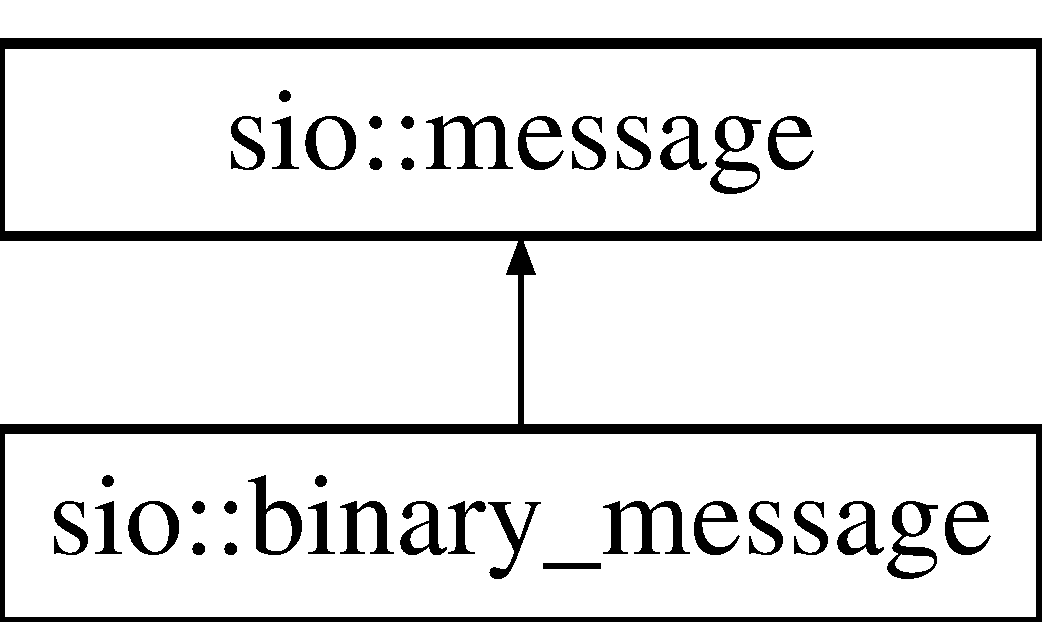
\includegraphics[height=2.000000cm]{classsio_1_1binary__message}
\end{center}
\end{figure}
\subsection*{Public Member Functions}
\begin{DoxyCompactItemize}
\item 
std\+::shared\+\_\+ptr$<$ const std\+::string $>$ const  \& \hyperlink{classsio_1_1binary__message_aac4db910fd9afb507ef0750394c5cd29}{get\+\_\+binary} () const
\end{DoxyCompactItemize}
\subsection*{Static Public Member Functions}
\begin{DoxyCompactItemize}
\item 
static \hyperlink{classsio_1_1message_a6340b6fef57e4516eb17928b1885a615}{message\+::ptr} \hyperlink{classsio_1_1binary__message_afd6bf4a5d9cd36a8082da4e4febfd60e}{create} (std\+::shared\+\_\+ptr$<$ const std\+::string $>$ const \&v)
\end{DoxyCompactItemize}
\subsection*{Additional Inherited Members}


\subsection{Member Function Documentation}
\mbox{\Hypertarget{classsio_1_1binary__message_afd6bf4a5d9cd36a8082da4e4febfd60e}\label{classsio_1_1binary__message_afd6bf4a5d9cd36a8082da4e4febfd60e}} 
\index{sio\+::binary\+\_\+message@{sio\+::binary\+\_\+message}!create@{create}}
\index{create@{create}!sio\+::binary\+\_\+message@{sio\+::binary\+\_\+message}}
\subsubsection{\texorpdfstring{create()}{create()}}
{\footnotesize\ttfamily static \hyperlink{classsio_1_1message_a6340b6fef57e4516eb17928b1885a615}{message\+::ptr} sio\+::binary\+\_\+message\+::create (\begin{DoxyParamCaption}\item[{std\+::shared\+\_\+ptr$<$ const std\+::string $>$ const \&}]{v }\end{DoxyParamCaption})\hspace{0.3cm}{\ttfamily [inline]}, {\ttfamily [static]}}

\mbox{\Hypertarget{classsio_1_1binary__message_aac4db910fd9afb507ef0750394c5cd29}\label{classsio_1_1binary__message_aac4db910fd9afb507ef0750394c5cd29}} 
\index{sio\+::binary\+\_\+message@{sio\+::binary\+\_\+message}!get\+\_\+binary@{get\+\_\+binary}}
\index{get\+\_\+binary@{get\+\_\+binary}!sio\+::binary\+\_\+message@{sio\+::binary\+\_\+message}}
\subsubsection{\texorpdfstring{get\+\_\+binary()}{get\_binary()}}
{\footnotesize\ttfamily std\+::shared\+\_\+ptr$<$const std\+::string$>$ const\& sio\+::binary\+\_\+message\+::get\+\_\+binary (\begin{DoxyParamCaption}{ }\end{DoxyParamCaption}) const\hspace{0.3cm}{\ttfamily [inline]}, {\ttfamily [virtual]}}



Reimplemented from \hyperlink{classsio_1_1message_a55b9eeeb305f46bbf21ae339501174c2}{sio\+::message}.



The documentation for this class was generated from the following file\+:\begin{DoxyCompactItemize}
\item 
/home/erik/work/bridges/bridges-\/cxx/src/\hyperlink{sio__message_8h}{sio\+\_\+message.\+h}\end{DoxyCompactItemize}

\hypertarget{classbridges_1_1datastructure_1_1_bin_tree_element}{}\section{bridges\+:\+:datastructure\+:\+:Bin\+Tree\+Element$<$ E $>$ Class Template Reference}
\label{classbridges_1_1datastructure_1_1_bin_tree_element}\index{bridges\+::datastructure\+::\+Bin\+Tree\+Element$<$ E $>$@{bridges\+::datastructure\+::\+Bin\+Tree\+Element$<$ E $>$}}


{\ttfamily \#include $<$Bin\+Tree\+Element.\+h$>$}

Inheritance diagram for bridges\+:\+:datastructure\+:\+:Bin\+Tree\+Element$<$ E $>$\+:\begin{figure}[H]
\begin{center}
\leavevmode
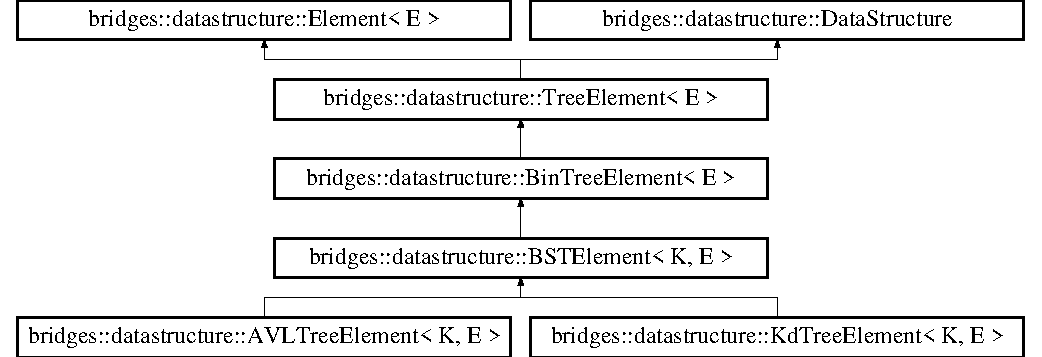
\includegraphics[height=4.794520cm]{classbridges_1_1datastructure_1_1_bin_tree_element}
\end{center}
\end{figure}


\subsection{Detailed Description}
\subsubsection*{template$<$typename E$>$\newline
class bridges\+::datastructure\+::\+Bin\+Tree\+Element$<$ E $>$}

This class can be used to create binary tree elements, derived from \hyperlink{classbridges_1_1datastructure_1_1_tree_element}{Tree\+Element}. 

This class can be used to create binary tree elements, with left and right children.

Generic Parameters\+: E the application data type

\begin{DoxyAuthor}{Author}
Kalpathi Subramanian 
\end{DoxyAuthor}
\begin{DoxyDate}{Date}
6/12/15, 7/12/19
\end{DoxyDate}
There is a tutorial about Binary Trees \+: \href{http://bridgesuncc.github.io/tutorials/BinTree.html}{\tt http\+://bridgesuncc.\+github.\+io/tutorials/\+Bin\+Tree.\+html} \subsection*{Public Member Functions}
\begin{DoxyCompactItemize}
\item 
\hyperlink{classbridges_1_1datastructure_1_1_bin_tree_element_aaea6c57206cffc0be3204b971fcaf5dd}{Bin\+Tree\+Element} (\hyperlink{classbridges_1_1datastructure_1_1_bin_tree_element}{Bin\+Tree\+Element} $\ast$l, \hyperlink{classbridges_1_1datastructure_1_1_bin_tree_element}{Bin\+Tree\+Element} $\ast$r, const E \&e=E(), const string \&lab=string())
\item 
\hyperlink{classbridges_1_1datastructure_1_1_bin_tree_element_a0f17a369aeb864ea52cfd25ba6b48e89}{Bin\+Tree\+Element} (const E \&e=E(), const string \&lab=string())
\item 
virtual const string \hyperlink{classbridges_1_1datastructure_1_1_bin_tree_element_aef86e3663785972251547e409fdc757b}{get\+D\+Stype} () const override
\item 
virtual \hyperlink{classbridges_1_1datastructure_1_1_bin_tree_element}{Bin\+Tree\+Element} $\ast$ \hyperlink{classbridges_1_1datastructure_1_1_bin_tree_element_ab30cfe373892c52709d5f1df013a0c82}{get\+Left} ()
\item 
virtual const \hyperlink{classbridges_1_1datastructure_1_1_bin_tree_element}{Bin\+Tree\+Element} $\ast$ \hyperlink{classbridges_1_1datastructure_1_1_bin_tree_element_ae14a70e2d25ad62337c87059b0cadb48}{get\+Left} () const
\item 
void \hyperlink{classbridges_1_1datastructure_1_1_bin_tree_element_a3b3caddd57fd31963b248b4dbcf3df27}{set\+Left} (\hyperlink{classbridges_1_1datastructure_1_1_bin_tree_element}{Bin\+Tree\+Element} $\ast$l)
\item 
virtual \hyperlink{classbridges_1_1datastructure_1_1_bin_tree_element}{Bin\+Tree\+Element} $\ast$ \hyperlink{classbridges_1_1datastructure_1_1_bin_tree_element_ae1e6bde8cc03cf5da5a7930354fdf592}{get\+Right} ()
\item 
virtual const \hyperlink{classbridges_1_1datastructure_1_1_bin_tree_element}{Bin\+Tree\+Element} $\ast$ \hyperlink{classbridges_1_1datastructure_1_1_bin_tree_element_a795b1696d628b55dafb2bc1aa961843a}{get\+Right} () const
\item 
void \hyperlink{classbridges_1_1datastructure_1_1_bin_tree_element_a59a1f7bac555e8a9bd88fd4aa1bd9b82}{set\+Right} (\hyperlink{classbridges_1_1datastructure_1_1_bin_tree_element}{Bin\+Tree\+Element} $\ast$r)
\end{DoxyCompactItemize}
\subsection*{Additional Inherited Members}


\subsection{Constructor \& Destructor Documentation}
\mbox{\Hypertarget{classbridges_1_1datastructure_1_1_bin_tree_element_aaea6c57206cffc0be3204b971fcaf5dd}\label{classbridges_1_1datastructure_1_1_bin_tree_element_aaea6c57206cffc0be3204b971fcaf5dd}} 
\index{bridges\+::datastructure\+::\+Bin\+Tree\+Element@{bridges\+::datastructure\+::\+Bin\+Tree\+Element}!Bin\+Tree\+Element@{Bin\+Tree\+Element}}
\index{Bin\+Tree\+Element@{Bin\+Tree\+Element}!bridges\+::datastructure\+::\+Bin\+Tree\+Element@{bridges\+::datastructure\+::\+Bin\+Tree\+Element}}
\subsubsection{\texorpdfstring{Bin\+Tree\+Element()}{BinTreeElement()}\hspace{0.1cm}{\footnotesize\ttfamily [1/2]}}
{\footnotesize\ttfamily template$<$typename E $>$ \\
\hyperlink{classbridges_1_1datastructure_1_1_bin_tree_element}{bridges\+::datastructure\+::\+Bin\+Tree\+Element}$<$ E $>$\+::\hyperlink{classbridges_1_1datastructure_1_1_bin_tree_element}{Bin\+Tree\+Element} (\begin{DoxyParamCaption}\item[{\hyperlink{classbridges_1_1datastructure_1_1_bin_tree_element}{Bin\+Tree\+Element}$<$ E $>$ $\ast$}]{l,  }\item[{\hyperlink{classbridges_1_1datastructure_1_1_bin_tree_element}{Bin\+Tree\+Element}$<$ E $>$ $\ast$}]{r,  }\item[{const E \&}]{e = {\ttfamily E()},  }\item[{const string \&}]{lab = {\ttfamily string()} }\end{DoxyParamCaption})\hspace{0.3cm}{\ttfamily [inline]}}

Constructs a \hyperlink{classbridges_1_1datastructure_1_1_bin_tree_element}{Bin\+Tree\+Element} with the provided value, label, left and right Bin\+Tree\+Elements. The defaults will be used if not provided.


\begin{DoxyParams}{Parameters}
{\em e} & The data to hold \\
\hline
{\em lab} & The label to show \\
\hline
{\em l} & The left \hyperlink{classbridges_1_1datastructure_1_1_tree_element}{Tree\+Element} \\
\hline
{\em r} & The right \hyperlink{classbridges_1_1datastructure_1_1_tree_element}{Tree\+Element} \\
\hline
\end{DoxyParams}
\mbox{\Hypertarget{classbridges_1_1datastructure_1_1_bin_tree_element_a0f17a369aeb864ea52cfd25ba6b48e89}\label{classbridges_1_1datastructure_1_1_bin_tree_element_a0f17a369aeb864ea52cfd25ba6b48e89}} 
\index{bridges\+::datastructure\+::\+Bin\+Tree\+Element@{bridges\+::datastructure\+::\+Bin\+Tree\+Element}!Bin\+Tree\+Element@{Bin\+Tree\+Element}}
\index{Bin\+Tree\+Element@{Bin\+Tree\+Element}!bridges\+::datastructure\+::\+Bin\+Tree\+Element@{bridges\+::datastructure\+::\+Bin\+Tree\+Element}}
\subsubsection{\texorpdfstring{Bin\+Tree\+Element()}{BinTreeElement()}\hspace{0.1cm}{\footnotesize\ttfamily [2/2]}}
{\footnotesize\ttfamily template$<$typename E $>$ \\
\hyperlink{classbridges_1_1datastructure_1_1_bin_tree_element}{bridges\+::datastructure\+::\+Bin\+Tree\+Element}$<$ E $>$\+::\hyperlink{classbridges_1_1datastructure_1_1_bin_tree_element}{Bin\+Tree\+Element} (\begin{DoxyParamCaption}\item[{const E \&}]{e = {\ttfamily E()},  }\item[{const string \&}]{lab = {\ttfamily string()} }\end{DoxyParamCaption})\hspace{0.3cm}{\ttfamily [inline]}}

Constructs a \hyperlink{classbridges_1_1datastructure_1_1_bin_tree_element}{Bin\+Tree\+Element} with the provided value and label, setting the left and right \hyperlink{classbridges_1_1datastructure_1_1_bin_tree_element}{Bin\+Tree\+Element} to N\+U\+LL. The defaults will be used if not provided.


\begin{DoxyParams}{Parameters}
{\em e} & The data to hold \\
\hline
{\em lab} & The label to show \\
\hline
\end{DoxyParams}


\subsection{Member Function Documentation}
\mbox{\Hypertarget{classbridges_1_1datastructure_1_1_bin_tree_element_aef86e3663785972251547e409fdc757b}\label{classbridges_1_1datastructure_1_1_bin_tree_element_aef86e3663785972251547e409fdc757b}} 
\index{bridges\+::datastructure\+::\+Bin\+Tree\+Element@{bridges\+::datastructure\+::\+Bin\+Tree\+Element}!get\+D\+Stype@{get\+D\+Stype}}
\index{get\+D\+Stype@{get\+D\+Stype}!bridges\+::datastructure\+::\+Bin\+Tree\+Element@{bridges\+::datastructure\+::\+Bin\+Tree\+Element}}
\subsubsection{\texorpdfstring{get\+D\+Stype()}{getDStype()}}
{\footnotesize\ttfamily template$<$typename E $>$ \\
virtual const string \hyperlink{classbridges_1_1datastructure_1_1_bin_tree_element}{bridges\+::datastructure\+::\+Bin\+Tree\+Element}$<$ E $>$\+::get\+D\+Stype (\begin{DoxyParamCaption}{ }\end{DoxyParamCaption}) const\hspace{0.3cm}{\ttfamily [inline]}, {\ttfamily [override]}, {\ttfamily [virtual]}}

\begin{DoxyReturn}{Returns}
the data structure type 
\end{DoxyReturn}


Reimplemented from \hyperlink{classbridges_1_1datastructure_1_1_tree_element_a897f34ea284da45e1dc869c3e3b6c9a4}{bridges\+::datastructure\+::\+Tree\+Element$<$ E $>$}.



Reimplemented in \hyperlink{classbridges_1_1datastructure_1_1_kd_tree_element_a76f6d9bfadfdec09d0a8564aa0e33235}{bridges\+::datastructure\+::\+Kd\+Tree\+Element$<$ K, E $>$}, \hyperlink{classbridges_1_1datastructure_1_1_b_s_t_element_a2bb8cc9ec4b6bc5b89ecef0f17be366f}{bridges\+::datastructure\+::\+B\+S\+T\+Element$<$ K, E $>$}, and \hyperlink{classbridges_1_1datastructure_1_1_a_v_l_tree_element_ab04d1e9ad4630e408041e8137dc9854a}{bridges\+::datastructure\+::\+A\+V\+L\+Tree\+Element$<$ K, E $>$}.

\mbox{\Hypertarget{classbridges_1_1datastructure_1_1_bin_tree_element_ab30cfe373892c52709d5f1df013a0c82}\label{classbridges_1_1datastructure_1_1_bin_tree_element_ab30cfe373892c52709d5f1df013a0c82}} 
\index{bridges\+::datastructure\+::\+Bin\+Tree\+Element@{bridges\+::datastructure\+::\+Bin\+Tree\+Element}!get\+Left@{get\+Left}}
\index{get\+Left@{get\+Left}!bridges\+::datastructure\+::\+Bin\+Tree\+Element@{bridges\+::datastructure\+::\+Bin\+Tree\+Element}}
\subsubsection{\texorpdfstring{get\+Left()}{getLeft()}\hspace{0.1cm}{\footnotesize\ttfamily [1/2]}}
{\footnotesize\ttfamily template$<$typename E $>$ \\
virtual \hyperlink{classbridges_1_1datastructure_1_1_bin_tree_element}{Bin\+Tree\+Element}$\ast$ \hyperlink{classbridges_1_1datastructure_1_1_bin_tree_element}{bridges\+::datastructure\+::\+Bin\+Tree\+Element}$<$ E $>$\+::get\+Left (\begin{DoxyParamCaption}{ }\end{DoxyParamCaption})\hspace{0.3cm}{\ttfamily [inline]}, {\ttfamily [virtual]}}

Returns the left child \begin{DoxyReturn}{Returns}
The left \hyperlink{classbridges_1_1datastructure_1_1_bin_tree_element}{Bin\+Tree\+Element} 
\end{DoxyReturn}


Reimplemented in \hyperlink{classbridges_1_1datastructure_1_1_kd_tree_element_a875bfa2dfd88a7740f7bcd28a117c12a}{bridges\+::datastructure\+::\+Kd\+Tree\+Element$<$ K, E $>$}, \hyperlink{classbridges_1_1datastructure_1_1_b_s_t_element_af863c624691c11db26ae3b6d723d1f5c}{bridges\+::datastructure\+::\+B\+S\+T\+Element$<$ K, E $>$}, and \hyperlink{classbridges_1_1datastructure_1_1_a_v_l_tree_element_ab05925e343b9fa71b61c71e8034e1293}{bridges\+::datastructure\+::\+A\+V\+L\+Tree\+Element$<$ K, E $>$}.

\mbox{\Hypertarget{classbridges_1_1datastructure_1_1_bin_tree_element_ae14a70e2d25ad62337c87059b0cadb48}\label{classbridges_1_1datastructure_1_1_bin_tree_element_ae14a70e2d25ad62337c87059b0cadb48}} 
\index{bridges\+::datastructure\+::\+Bin\+Tree\+Element@{bridges\+::datastructure\+::\+Bin\+Tree\+Element}!get\+Left@{get\+Left}}
\index{get\+Left@{get\+Left}!bridges\+::datastructure\+::\+Bin\+Tree\+Element@{bridges\+::datastructure\+::\+Bin\+Tree\+Element}}
\subsubsection{\texorpdfstring{get\+Left()}{getLeft()}\hspace{0.1cm}{\footnotesize\ttfamily [2/2]}}
{\footnotesize\ttfamily template$<$typename E $>$ \\
virtual const \hyperlink{classbridges_1_1datastructure_1_1_bin_tree_element}{Bin\+Tree\+Element}$\ast$ \hyperlink{classbridges_1_1datastructure_1_1_bin_tree_element}{bridges\+::datastructure\+::\+Bin\+Tree\+Element}$<$ E $>$\+::get\+Left (\begin{DoxyParamCaption}{ }\end{DoxyParamCaption}) const\hspace{0.3cm}{\ttfamily [inline]}, {\ttfamily [virtual]}}

Returns the left child -\/ Constant version \begin{DoxyReturn}{Returns}
The left \hyperlink{classbridges_1_1datastructure_1_1_bin_tree_element}{Bin\+Tree\+Element} 
\end{DoxyReturn}


Reimplemented in \hyperlink{classbridges_1_1datastructure_1_1_kd_tree_element_a653597918fbc6e31b84fcf8dbdf67122}{bridges\+::datastructure\+::\+Kd\+Tree\+Element$<$ K, E $>$}, \hyperlink{classbridges_1_1datastructure_1_1_b_s_t_element_abac324ef0b480420bd82ecfe4501d60d}{bridges\+::datastructure\+::\+B\+S\+T\+Element$<$ K, E $>$}, and \hyperlink{classbridges_1_1datastructure_1_1_a_v_l_tree_element_a4a639e0c623435aadf5c51ed132cb25d}{bridges\+::datastructure\+::\+A\+V\+L\+Tree\+Element$<$ K, E $>$}.

\mbox{\Hypertarget{classbridges_1_1datastructure_1_1_bin_tree_element_ae1e6bde8cc03cf5da5a7930354fdf592}\label{classbridges_1_1datastructure_1_1_bin_tree_element_ae1e6bde8cc03cf5da5a7930354fdf592}} 
\index{bridges\+::datastructure\+::\+Bin\+Tree\+Element@{bridges\+::datastructure\+::\+Bin\+Tree\+Element}!get\+Right@{get\+Right}}
\index{get\+Right@{get\+Right}!bridges\+::datastructure\+::\+Bin\+Tree\+Element@{bridges\+::datastructure\+::\+Bin\+Tree\+Element}}
\subsubsection{\texorpdfstring{get\+Right()}{getRight()}\hspace{0.1cm}{\footnotesize\ttfamily [1/2]}}
{\footnotesize\ttfamily template$<$typename E $>$ \\
virtual \hyperlink{classbridges_1_1datastructure_1_1_bin_tree_element}{Bin\+Tree\+Element}$\ast$ \hyperlink{classbridges_1_1datastructure_1_1_bin_tree_element}{bridges\+::datastructure\+::\+Bin\+Tree\+Element}$<$ E $>$\+::get\+Right (\begin{DoxyParamCaption}{ }\end{DoxyParamCaption})\hspace{0.3cm}{\ttfamily [inline]}, {\ttfamily [virtual]}}

Returns the right child \begin{DoxyReturn}{Returns}
The right \hyperlink{classbridges_1_1datastructure_1_1_bin_tree_element}{Bin\+Tree\+Element} 
\end{DoxyReturn}


Reimplemented in \hyperlink{classbridges_1_1datastructure_1_1_kd_tree_element_a366e3b0987169220d3a145043be2373d}{bridges\+::datastructure\+::\+Kd\+Tree\+Element$<$ K, E $>$}, \hyperlink{classbridges_1_1datastructure_1_1_b_s_t_element_a80f5085d6d03805dd3091b7693d8e235}{bridges\+::datastructure\+::\+B\+S\+T\+Element$<$ K, E $>$}, and \hyperlink{classbridges_1_1datastructure_1_1_a_v_l_tree_element_aed585fdf56fcbfebac6cd0262c9c1807}{bridges\+::datastructure\+::\+A\+V\+L\+Tree\+Element$<$ K, E $>$}.

\mbox{\Hypertarget{classbridges_1_1datastructure_1_1_bin_tree_element_a795b1696d628b55dafb2bc1aa961843a}\label{classbridges_1_1datastructure_1_1_bin_tree_element_a795b1696d628b55dafb2bc1aa961843a}} 
\index{bridges\+::datastructure\+::\+Bin\+Tree\+Element@{bridges\+::datastructure\+::\+Bin\+Tree\+Element}!get\+Right@{get\+Right}}
\index{get\+Right@{get\+Right}!bridges\+::datastructure\+::\+Bin\+Tree\+Element@{bridges\+::datastructure\+::\+Bin\+Tree\+Element}}
\subsubsection{\texorpdfstring{get\+Right()}{getRight()}\hspace{0.1cm}{\footnotesize\ttfamily [2/2]}}
{\footnotesize\ttfamily template$<$typename E $>$ \\
virtual const \hyperlink{classbridges_1_1datastructure_1_1_bin_tree_element}{Bin\+Tree\+Element}$\ast$ \hyperlink{classbridges_1_1datastructure_1_1_bin_tree_element}{bridges\+::datastructure\+::\+Bin\+Tree\+Element}$<$ E $>$\+::get\+Right (\begin{DoxyParamCaption}{ }\end{DoxyParamCaption}) const\hspace{0.3cm}{\ttfamily [inline]}, {\ttfamily [virtual]}}

Returns the right child -\/ Constant version \begin{DoxyReturn}{Returns}
The right \hyperlink{classbridges_1_1datastructure_1_1_bin_tree_element}{Bin\+Tree\+Element} 
\end{DoxyReturn}


Reimplemented in \hyperlink{classbridges_1_1datastructure_1_1_kd_tree_element_ae8d6007d3848b72cbfc11d2e29120781}{bridges\+::datastructure\+::\+Kd\+Tree\+Element$<$ K, E $>$}, \hyperlink{classbridges_1_1datastructure_1_1_b_s_t_element_a012f0eb09c3d62b14c73109e6ded0879}{bridges\+::datastructure\+::\+B\+S\+T\+Element$<$ K, E $>$}, and \hyperlink{classbridges_1_1datastructure_1_1_a_v_l_tree_element_a5a2c4b96b51da1daa3c0426882250acb}{bridges\+::datastructure\+::\+A\+V\+L\+Tree\+Element$<$ K, E $>$}.

\mbox{\Hypertarget{classbridges_1_1datastructure_1_1_bin_tree_element_a3b3caddd57fd31963b248b4dbcf3df27}\label{classbridges_1_1datastructure_1_1_bin_tree_element_a3b3caddd57fd31963b248b4dbcf3df27}} 
\index{bridges\+::datastructure\+::\+Bin\+Tree\+Element@{bridges\+::datastructure\+::\+Bin\+Tree\+Element}!set\+Left@{set\+Left}}
\index{set\+Left@{set\+Left}!bridges\+::datastructure\+::\+Bin\+Tree\+Element@{bridges\+::datastructure\+::\+Bin\+Tree\+Element}}
\subsubsection{\texorpdfstring{set\+Left()}{setLeft()}}
{\footnotesize\ttfamily template$<$typename E $>$ \\
void \hyperlink{classbridges_1_1datastructure_1_1_bin_tree_element}{bridges\+::datastructure\+::\+Bin\+Tree\+Element}$<$ E $>$\+::set\+Left (\begin{DoxyParamCaption}\item[{\hyperlink{classbridges_1_1datastructure_1_1_bin_tree_element}{Bin\+Tree\+Element}$<$ E $>$ $\ast$}]{l }\end{DoxyParamCaption})\hspace{0.3cm}{\ttfamily [inline]}}

Sets left child to \char`\"{}l\char`\"{}


\begin{DoxyParams}{Parameters}
{\em l} & left child pointer \\
\hline
\end{DoxyParams}
\mbox{\Hypertarget{classbridges_1_1datastructure_1_1_bin_tree_element_a59a1f7bac555e8a9bd88fd4aa1bd9b82}\label{classbridges_1_1datastructure_1_1_bin_tree_element_a59a1f7bac555e8a9bd88fd4aa1bd9b82}} 
\index{bridges\+::datastructure\+::\+Bin\+Tree\+Element@{bridges\+::datastructure\+::\+Bin\+Tree\+Element}!set\+Right@{set\+Right}}
\index{set\+Right@{set\+Right}!bridges\+::datastructure\+::\+Bin\+Tree\+Element@{bridges\+::datastructure\+::\+Bin\+Tree\+Element}}
\subsubsection{\texorpdfstring{set\+Right()}{setRight()}}
{\footnotesize\ttfamily template$<$typename E $>$ \\
void \hyperlink{classbridges_1_1datastructure_1_1_bin_tree_element}{bridges\+::datastructure\+::\+Bin\+Tree\+Element}$<$ E $>$\+::set\+Right (\begin{DoxyParamCaption}\item[{\hyperlink{classbridges_1_1datastructure_1_1_bin_tree_element}{Bin\+Tree\+Element}$<$ E $>$ $\ast$}]{r }\end{DoxyParamCaption})\hspace{0.3cm}{\ttfamily [inline]}}

Sets right to \char`\"{}r\char`\"{}


\begin{DoxyParams}{Parameters}
{\em r} & right child pointer \\
\hline
\end{DoxyParams}


The documentation for this class was generated from the following file\+:\begin{DoxyCompactItemize}
\item 
/home/erik/work/bridges/bridges-\/cxx/src/\hyperlink{_bin_tree_element_8h}{Bin\+Tree\+Element.\+h}\end{DoxyCompactItemize}

\hypertarget{classbridges_1_1dataset_1_1_book}{}\section{bridges\+:\+:dataset\+:\+:Book Class Reference}
\label{classbridges_1_1dataset_1_1_book}\index{bridges\+::dataset\+::\+Book@{bridges\+::dataset\+::\+Book}}


{\ttfamily \#include $<$Book.\+h$>$}



\subsection{Detailed Description}
A \hyperlink{classbridges_1_1dataset_1_1_book}{Book} object, used along with the books data source. 

This is a convenience class provided for users who wish to use this data source as part of their application. It provides an A\+PI that makes it easy to access the attributes of this data set.

Refer to tutorial examples to using this data source in data structure assignments.

\begin{DoxyAuthor}{Author}
Kalpathi Subramanian 
\end{DoxyAuthor}
\begin{DoxyDate}{Date}
1/16/17 
\end{DoxyDate}
\subsection*{Public Member Functions}
\begin{DoxyCompactItemize}
\item 
\hyperlink{classbridges_1_1dataset_1_1_book_a951e7d455f2fd89aa05224cbf362e244}{Book} ()
\item 
\hyperlink{classbridges_1_1dataset_1_1_book_a4770a401c2634cb9124c34e462721338}{Book} (const string \&author\+Name, int author\+Birth, int author\+Death, const string \&title, const vector$<$ string $>$ \&lang, const vector$<$ string $>$ \&genre, const vector$<$ string $>$ \&subject, int num\+Chars, int num\+Words, int num\+Sentences, int num\+Difficult\+Words, const string \&url, int downloads)
\item 
string \hyperlink{classbridges_1_1dataset_1_1_book_ad2a683f09b76c7262c3de0215bf2f40d}{get\+Author\+Name} () const
\item 
void \hyperlink{classbridges_1_1dataset_1_1_book_a6a361133defe82e2405af865514a0065}{set\+Author\+Name} (const string \&author\+Name)
\item 
int \hyperlink{classbridges_1_1dataset_1_1_book_aa7ba093d9bf5ee7d757a0b8ff87e06f0}{get\+Author\+Birth} () const
\item 
void \hyperlink{classbridges_1_1dataset_1_1_book_a04c01f0f2f0778f7f5c6bde3f98e0608}{set\+Author\+Birth} (int author\+Birth)
\item 
int \hyperlink{classbridges_1_1dataset_1_1_book_ac4cfa9060e1d9cedbf2143215065a3ed}{get\+Author\+Death} () const
\item 
void \hyperlink{classbridges_1_1dataset_1_1_book_a318b060a519e1889507a20313683ed89}{set\+Author\+Death} (int author\+Death)
\item 
string \hyperlink{classbridges_1_1dataset_1_1_book_a3c4ca2e8bfa41fb502a5343b586dc73f}{get\+Title} () const
\item 
void \hyperlink{classbridges_1_1dataset_1_1_book_a19015494ad6a1d9c75a5c6af63be0dbf}{set\+Title} (const string \&title)
\item 
vector$<$ string $>$ \hyperlink{classbridges_1_1dataset_1_1_book_ae9df8dfb356a6b84977118a64d2982ad}{get\+Lang} () const
\item 
void \hyperlink{classbridges_1_1dataset_1_1_book_aa3b75d6178efc4ddef9b3255dafba3ab}{set\+Lang} (const vector$<$ string $>$ \&lang)
\item 
vector$<$ string $>$ \hyperlink{classbridges_1_1dataset_1_1_book_a26554290984472af3e3dbb9b138e6750}{get\+Genre} () const
\item 
void \hyperlink{classbridges_1_1dataset_1_1_book_a3acd969bba59827fb4e099565e7076bf}{set\+Genre} (const vector$<$ string $>$ \&genre)
\item 
vector$<$ string $>$ \hyperlink{classbridges_1_1dataset_1_1_book_ad68e9b4da931d1a1328fe1ee41acaa58}{get\+Subject} () const
\item 
void \hyperlink{classbridges_1_1dataset_1_1_book_a1473fa37374bbd66561fa02b7ff0d5cf}{set\+Subject} (const vector$<$ string $>$ \&subject)
\item 
string \hyperlink{classbridges_1_1dataset_1_1_book_a5e7dff3aad5acf540f8b0c487fd903a3}{get\+U\+RL} () const
\item 
void \hyperlink{classbridges_1_1dataset_1_1_book_a4d984e8854164f18944198293759319e}{set\+U\+RL} (const string \&url)
\item 
int \hyperlink{classbridges_1_1dataset_1_1_book_af8836440c237f2b8b7a9a0bd11c41d99}{get\+Num\+Chars} () const
\item 
void \hyperlink{classbridges_1_1dataset_1_1_book_af8dea379bd5a00af2257ce565ed6b643}{set\+Num\+Chars} (int num\+Chars)
\item 
int \hyperlink{classbridges_1_1dataset_1_1_book_a087d17660090ce28fbe7245094fb1711}{get\+Num\+Words} () const
\item 
void \hyperlink{classbridges_1_1dataset_1_1_book_afc1d3c8db63d4525e5070e61db5be7e1}{set\+Num\+Words} (int num\+Words)
\item 
int \hyperlink{classbridges_1_1dataset_1_1_book_a7a1b5fef3b464586e635a7444a9e4e41}{get\+Num\+Sentences} () const
\item 
void \hyperlink{classbridges_1_1dataset_1_1_book_a55be4872ed29dc79cdbe56189db6e5e6}{set\+Num\+Sentences} (int num\+Sentences)
\item 
int \hyperlink{classbridges_1_1dataset_1_1_book_aee63718cb1343108d9b7dd66cef208cb}{get\+Num\+Difficult\+Words} () const
\item 
void \hyperlink{classbridges_1_1dataset_1_1_book_a7974e9966b289f897f76dba445f5859e}{set\+Num\+Difficult\+Words} (int num\+Difficult\+Words)
\item 
int \hyperlink{classbridges_1_1dataset_1_1_book_afc1c412c45d2a07b3d5f074e4bbd353a}{get\+Downloads} () const
\item 
void \hyperlink{classbridges_1_1dataset_1_1_book_a998370a590bc5128faa755b5b7c1a85b}{set\+Downloads} (int downloads)
\end{DoxyCompactItemize}


\subsection{Constructor \& Destructor Documentation}
\mbox{\Hypertarget{classbridges_1_1dataset_1_1_book_a951e7d455f2fd89aa05224cbf362e244}\label{classbridges_1_1dataset_1_1_book_a951e7d455f2fd89aa05224cbf362e244}} 
\index{bridges\+::dataset\+::\+Book@{bridges\+::dataset\+::\+Book}!Book@{Book}}
\index{Book@{Book}!bridges\+::dataset\+::\+Book@{bridges\+::dataset\+::\+Book}}
\subsubsection{\texorpdfstring{Book()}{Book()}\hspace{0.1cm}{\footnotesize\ttfamily [1/2]}}
{\footnotesize\ttfamily bridges\+::dataset\+::\+Book\+::\+Book (\begin{DoxyParamCaption}{ }\end{DoxyParamCaption})\hspace{0.3cm}{\ttfamily [inline]}}

\mbox{\Hypertarget{classbridges_1_1dataset_1_1_book_a4770a401c2634cb9124c34e462721338}\label{classbridges_1_1dataset_1_1_book_a4770a401c2634cb9124c34e462721338}} 
\index{bridges\+::dataset\+::\+Book@{bridges\+::dataset\+::\+Book}!Book@{Book}}
\index{Book@{Book}!bridges\+::dataset\+::\+Book@{bridges\+::dataset\+::\+Book}}
\subsubsection{\texorpdfstring{Book()}{Book()}\hspace{0.1cm}{\footnotesize\ttfamily [2/2]}}
{\footnotesize\ttfamily bridges\+::dataset\+::\+Book\+::\+Book (\begin{DoxyParamCaption}\item[{const string \&}]{author\+Name,  }\item[{int}]{author\+Birth,  }\item[{int}]{author\+Death,  }\item[{const string \&}]{title,  }\item[{const vector$<$ string $>$ \&}]{lang,  }\item[{const vector$<$ string $>$ \&}]{genre,  }\item[{const vector$<$ string $>$ \&}]{subject,  }\item[{int}]{num\+Chars,  }\item[{int}]{num\+Words,  }\item[{int}]{num\+Sentences,  }\item[{int}]{num\+Difficult\+Words,  }\item[{const string \&}]{url,  }\item[{int}]{downloads }\end{DoxyParamCaption})\hspace{0.3cm}{\ttfamily [inline]}}



\subsection{Member Function Documentation}
\mbox{\Hypertarget{classbridges_1_1dataset_1_1_book_aa7ba093d9bf5ee7d757a0b8ff87e06f0}\label{classbridges_1_1dataset_1_1_book_aa7ba093d9bf5ee7d757a0b8ff87e06f0}} 
\index{bridges\+::dataset\+::\+Book@{bridges\+::dataset\+::\+Book}!get\+Author\+Birth@{get\+Author\+Birth}}
\index{get\+Author\+Birth@{get\+Author\+Birth}!bridges\+::dataset\+::\+Book@{bridges\+::dataset\+::\+Book}}
\subsubsection{\texorpdfstring{get\+Author\+Birth()}{getAuthorBirth()}}
{\footnotesize\ttfamily int bridges\+::dataset\+::\+Book\+::get\+Author\+Birth (\begin{DoxyParamCaption}{ }\end{DoxyParamCaption}) const\hspace{0.3cm}{\ttfamily [inline]}}

\mbox{\Hypertarget{classbridges_1_1dataset_1_1_book_ac4cfa9060e1d9cedbf2143215065a3ed}\label{classbridges_1_1dataset_1_1_book_ac4cfa9060e1d9cedbf2143215065a3ed}} 
\index{bridges\+::dataset\+::\+Book@{bridges\+::dataset\+::\+Book}!get\+Author\+Death@{get\+Author\+Death}}
\index{get\+Author\+Death@{get\+Author\+Death}!bridges\+::dataset\+::\+Book@{bridges\+::dataset\+::\+Book}}
\subsubsection{\texorpdfstring{get\+Author\+Death()}{getAuthorDeath()}}
{\footnotesize\ttfamily int bridges\+::dataset\+::\+Book\+::get\+Author\+Death (\begin{DoxyParamCaption}{ }\end{DoxyParamCaption}) const\hspace{0.3cm}{\ttfamily [inline]}}

\mbox{\Hypertarget{classbridges_1_1dataset_1_1_book_ad2a683f09b76c7262c3de0215bf2f40d}\label{classbridges_1_1dataset_1_1_book_ad2a683f09b76c7262c3de0215bf2f40d}} 
\index{bridges\+::dataset\+::\+Book@{bridges\+::dataset\+::\+Book}!get\+Author\+Name@{get\+Author\+Name}}
\index{get\+Author\+Name@{get\+Author\+Name}!bridges\+::dataset\+::\+Book@{bridges\+::dataset\+::\+Book}}
\subsubsection{\texorpdfstring{get\+Author\+Name()}{getAuthorName()}}
{\footnotesize\ttfamily string bridges\+::dataset\+::\+Book\+::get\+Author\+Name (\begin{DoxyParamCaption}{ }\end{DoxyParamCaption}) const\hspace{0.3cm}{\ttfamily [inline]}}

\mbox{\Hypertarget{classbridges_1_1dataset_1_1_book_afc1c412c45d2a07b3d5f074e4bbd353a}\label{classbridges_1_1dataset_1_1_book_afc1c412c45d2a07b3d5f074e4bbd353a}} 
\index{bridges\+::dataset\+::\+Book@{bridges\+::dataset\+::\+Book}!get\+Downloads@{get\+Downloads}}
\index{get\+Downloads@{get\+Downloads}!bridges\+::dataset\+::\+Book@{bridges\+::dataset\+::\+Book}}
\subsubsection{\texorpdfstring{get\+Downloads()}{getDownloads()}}
{\footnotesize\ttfamily int bridges\+::dataset\+::\+Book\+::get\+Downloads (\begin{DoxyParamCaption}{ }\end{DoxyParamCaption}) const\hspace{0.3cm}{\ttfamily [inline]}}

\mbox{\Hypertarget{classbridges_1_1dataset_1_1_book_a26554290984472af3e3dbb9b138e6750}\label{classbridges_1_1dataset_1_1_book_a26554290984472af3e3dbb9b138e6750}} 
\index{bridges\+::dataset\+::\+Book@{bridges\+::dataset\+::\+Book}!get\+Genre@{get\+Genre}}
\index{get\+Genre@{get\+Genre}!bridges\+::dataset\+::\+Book@{bridges\+::dataset\+::\+Book}}
\subsubsection{\texorpdfstring{get\+Genre()}{getGenre()}}
{\footnotesize\ttfamily vector$<$string$>$ bridges\+::dataset\+::\+Book\+::get\+Genre (\begin{DoxyParamCaption}{ }\end{DoxyParamCaption}) const\hspace{0.3cm}{\ttfamily [inline]}}

\mbox{\Hypertarget{classbridges_1_1dataset_1_1_book_ae9df8dfb356a6b84977118a64d2982ad}\label{classbridges_1_1dataset_1_1_book_ae9df8dfb356a6b84977118a64d2982ad}} 
\index{bridges\+::dataset\+::\+Book@{bridges\+::dataset\+::\+Book}!get\+Lang@{get\+Lang}}
\index{get\+Lang@{get\+Lang}!bridges\+::dataset\+::\+Book@{bridges\+::dataset\+::\+Book}}
\subsubsection{\texorpdfstring{get\+Lang()}{getLang()}}
{\footnotesize\ttfamily vector$<$string$>$ bridges\+::dataset\+::\+Book\+::get\+Lang (\begin{DoxyParamCaption}{ }\end{DoxyParamCaption}) const\hspace{0.3cm}{\ttfamily [inline]}}

\mbox{\Hypertarget{classbridges_1_1dataset_1_1_book_af8836440c237f2b8b7a9a0bd11c41d99}\label{classbridges_1_1dataset_1_1_book_af8836440c237f2b8b7a9a0bd11c41d99}} 
\index{bridges\+::dataset\+::\+Book@{bridges\+::dataset\+::\+Book}!get\+Num\+Chars@{get\+Num\+Chars}}
\index{get\+Num\+Chars@{get\+Num\+Chars}!bridges\+::dataset\+::\+Book@{bridges\+::dataset\+::\+Book}}
\subsubsection{\texorpdfstring{get\+Num\+Chars()}{getNumChars()}}
{\footnotesize\ttfamily int bridges\+::dataset\+::\+Book\+::get\+Num\+Chars (\begin{DoxyParamCaption}{ }\end{DoxyParamCaption}) const\hspace{0.3cm}{\ttfamily [inline]}}

\mbox{\Hypertarget{classbridges_1_1dataset_1_1_book_aee63718cb1343108d9b7dd66cef208cb}\label{classbridges_1_1dataset_1_1_book_aee63718cb1343108d9b7dd66cef208cb}} 
\index{bridges\+::dataset\+::\+Book@{bridges\+::dataset\+::\+Book}!get\+Num\+Difficult\+Words@{get\+Num\+Difficult\+Words}}
\index{get\+Num\+Difficult\+Words@{get\+Num\+Difficult\+Words}!bridges\+::dataset\+::\+Book@{bridges\+::dataset\+::\+Book}}
\subsubsection{\texorpdfstring{get\+Num\+Difficult\+Words()}{getNumDifficultWords()}}
{\footnotesize\ttfamily int bridges\+::dataset\+::\+Book\+::get\+Num\+Difficult\+Words (\begin{DoxyParamCaption}{ }\end{DoxyParamCaption}) const\hspace{0.3cm}{\ttfamily [inline]}}

\mbox{\Hypertarget{classbridges_1_1dataset_1_1_book_a7a1b5fef3b464586e635a7444a9e4e41}\label{classbridges_1_1dataset_1_1_book_a7a1b5fef3b464586e635a7444a9e4e41}} 
\index{bridges\+::dataset\+::\+Book@{bridges\+::dataset\+::\+Book}!get\+Num\+Sentences@{get\+Num\+Sentences}}
\index{get\+Num\+Sentences@{get\+Num\+Sentences}!bridges\+::dataset\+::\+Book@{bridges\+::dataset\+::\+Book}}
\subsubsection{\texorpdfstring{get\+Num\+Sentences()}{getNumSentences()}}
{\footnotesize\ttfamily int bridges\+::dataset\+::\+Book\+::get\+Num\+Sentences (\begin{DoxyParamCaption}{ }\end{DoxyParamCaption}) const\hspace{0.3cm}{\ttfamily [inline]}}

\mbox{\Hypertarget{classbridges_1_1dataset_1_1_book_a087d17660090ce28fbe7245094fb1711}\label{classbridges_1_1dataset_1_1_book_a087d17660090ce28fbe7245094fb1711}} 
\index{bridges\+::dataset\+::\+Book@{bridges\+::dataset\+::\+Book}!get\+Num\+Words@{get\+Num\+Words}}
\index{get\+Num\+Words@{get\+Num\+Words}!bridges\+::dataset\+::\+Book@{bridges\+::dataset\+::\+Book}}
\subsubsection{\texorpdfstring{get\+Num\+Words()}{getNumWords()}}
{\footnotesize\ttfamily int bridges\+::dataset\+::\+Book\+::get\+Num\+Words (\begin{DoxyParamCaption}{ }\end{DoxyParamCaption}) const\hspace{0.3cm}{\ttfamily [inline]}}

\mbox{\Hypertarget{classbridges_1_1dataset_1_1_book_ad68e9b4da931d1a1328fe1ee41acaa58}\label{classbridges_1_1dataset_1_1_book_ad68e9b4da931d1a1328fe1ee41acaa58}} 
\index{bridges\+::dataset\+::\+Book@{bridges\+::dataset\+::\+Book}!get\+Subject@{get\+Subject}}
\index{get\+Subject@{get\+Subject}!bridges\+::dataset\+::\+Book@{bridges\+::dataset\+::\+Book}}
\subsubsection{\texorpdfstring{get\+Subject()}{getSubject()}}
{\footnotesize\ttfamily vector$<$string$>$ bridges\+::dataset\+::\+Book\+::get\+Subject (\begin{DoxyParamCaption}{ }\end{DoxyParamCaption}) const\hspace{0.3cm}{\ttfamily [inline]}}

\mbox{\Hypertarget{classbridges_1_1dataset_1_1_book_a3c4ca2e8bfa41fb502a5343b586dc73f}\label{classbridges_1_1dataset_1_1_book_a3c4ca2e8bfa41fb502a5343b586dc73f}} 
\index{bridges\+::dataset\+::\+Book@{bridges\+::dataset\+::\+Book}!get\+Title@{get\+Title}}
\index{get\+Title@{get\+Title}!bridges\+::dataset\+::\+Book@{bridges\+::dataset\+::\+Book}}
\subsubsection{\texorpdfstring{get\+Title()}{getTitle()}}
{\footnotesize\ttfamily string bridges\+::dataset\+::\+Book\+::get\+Title (\begin{DoxyParamCaption}{ }\end{DoxyParamCaption}) const\hspace{0.3cm}{\ttfamily [inline]}}

\mbox{\Hypertarget{classbridges_1_1dataset_1_1_book_a5e7dff3aad5acf540f8b0c487fd903a3}\label{classbridges_1_1dataset_1_1_book_a5e7dff3aad5acf540f8b0c487fd903a3}} 
\index{bridges\+::dataset\+::\+Book@{bridges\+::dataset\+::\+Book}!get\+U\+RL@{get\+U\+RL}}
\index{get\+U\+RL@{get\+U\+RL}!bridges\+::dataset\+::\+Book@{bridges\+::dataset\+::\+Book}}
\subsubsection{\texorpdfstring{get\+U\+R\+L()}{getURL()}}
{\footnotesize\ttfamily string bridges\+::dataset\+::\+Book\+::get\+U\+RL (\begin{DoxyParamCaption}{ }\end{DoxyParamCaption}) const\hspace{0.3cm}{\ttfamily [inline]}}

\mbox{\Hypertarget{classbridges_1_1dataset_1_1_book_a04c01f0f2f0778f7f5c6bde3f98e0608}\label{classbridges_1_1dataset_1_1_book_a04c01f0f2f0778f7f5c6bde3f98e0608}} 
\index{bridges\+::dataset\+::\+Book@{bridges\+::dataset\+::\+Book}!set\+Author\+Birth@{set\+Author\+Birth}}
\index{set\+Author\+Birth@{set\+Author\+Birth}!bridges\+::dataset\+::\+Book@{bridges\+::dataset\+::\+Book}}
\subsubsection{\texorpdfstring{set\+Author\+Birth()}{setAuthorBirth()}}
{\footnotesize\ttfamily void bridges\+::dataset\+::\+Book\+::set\+Author\+Birth (\begin{DoxyParamCaption}\item[{int}]{author\+Birth }\end{DoxyParamCaption})\hspace{0.3cm}{\ttfamily [inline]}}

\mbox{\Hypertarget{classbridges_1_1dataset_1_1_book_a318b060a519e1889507a20313683ed89}\label{classbridges_1_1dataset_1_1_book_a318b060a519e1889507a20313683ed89}} 
\index{bridges\+::dataset\+::\+Book@{bridges\+::dataset\+::\+Book}!set\+Author\+Death@{set\+Author\+Death}}
\index{set\+Author\+Death@{set\+Author\+Death}!bridges\+::dataset\+::\+Book@{bridges\+::dataset\+::\+Book}}
\subsubsection{\texorpdfstring{set\+Author\+Death()}{setAuthorDeath()}}
{\footnotesize\ttfamily void bridges\+::dataset\+::\+Book\+::set\+Author\+Death (\begin{DoxyParamCaption}\item[{int}]{author\+Death }\end{DoxyParamCaption})\hspace{0.3cm}{\ttfamily [inline]}}

\mbox{\Hypertarget{classbridges_1_1dataset_1_1_book_a6a361133defe82e2405af865514a0065}\label{classbridges_1_1dataset_1_1_book_a6a361133defe82e2405af865514a0065}} 
\index{bridges\+::dataset\+::\+Book@{bridges\+::dataset\+::\+Book}!set\+Author\+Name@{set\+Author\+Name}}
\index{set\+Author\+Name@{set\+Author\+Name}!bridges\+::dataset\+::\+Book@{bridges\+::dataset\+::\+Book}}
\subsubsection{\texorpdfstring{set\+Author\+Name()}{setAuthorName()}}
{\footnotesize\ttfamily void bridges\+::dataset\+::\+Book\+::set\+Author\+Name (\begin{DoxyParamCaption}\item[{const string \&}]{author\+Name }\end{DoxyParamCaption})\hspace{0.3cm}{\ttfamily [inline]}}

\mbox{\Hypertarget{classbridges_1_1dataset_1_1_book_a998370a590bc5128faa755b5b7c1a85b}\label{classbridges_1_1dataset_1_1_book_a998370a590bc5128faa755b5b7c1a85b}} 
\index{bridges\+::dataset\+::\+Book@{bridges\+::dataset\+::\+Book}!set\+Downloads@{set\+Downloads}}
\index{set\+Downloads@{set\+Downloads}!bridges\+::dataset\+::\+Book@{bridges\+::dataset\+::\+Book}}
\subsubsection{\texorpdfstring{set\+Downloads()}{setDownloads()}}
{\footnotesize\ttfamily void bridges\+::dataset\+::\+Book\+::set\+Downloads (\begin{DoxyParamCaption}\item[{int}]{downloads }\end{DoxyParamCaption})\hspace{0.3cm}{\ttfamily [inline]}}

\mbox{\Hypertarget{classbridges_1_1dataset_1_1_book_a3acd969bba59827fb4e099565e7076bf}\label{classbridges_1_1dataset_1_1_book_a3acd969bba59827fb4e099565e7076bf}} 
\index{bridges\+::dataset\+::\+Book@{bridges\+::dataset\+::\+Book}!set\+Genre@{set\+Genre}}
\index{set\+Genre@{set\+Genre}!bridges\+::dataset\+::\+Book@{bridges\+::dataset\+::\+Book}}
\subsubsection{\texorpdfstring{set\+Genre()}{setGenre()}}
{\footnotesize\ttfamily void bridges\+::dataset\+::\+Book\+::set\+Genre (\begin{DoxyParamCaption}\item[{const vector$<$ string $>$ \&}]{genre }\end{DoxyParamCaption})\hspace{0.3cm}{\ttfamily [inline]}}

\mbox{\Hypertarget{classbridges_1_1dataset_1_1_book_aa3b75d6178efc4ddef9b3255dafba3ab}\label{classbridges_1_1dataset_1_1_book_aa3b75d6178efc4ddef9b3255dafba3ab}} 
\index{bridges\+::dataset\+::\+Book@{bridges\+::dataset\+::\+Book}!set\+Lang@{set\+Lang}}
\index{set\+Lang@{set\+Lang}!bridges\+::dataset\+::\+Book@{bridges\+::dataset\+::\+Book}}
\subsubsection{\texorpdfstring{set\+Lang()}{setLang()}}
{\footnotesize\ttfamily void bridges\+::dataset\+::\+Book\+::set\+Lang (\begin{DoxyParamCaption}\item[{const vector$<$ string $>$ \&}]{lang }\end{DoxyParamCaption})\hspace{0.3cm}{\ttfamily [inline]}}

\mbox{\Hypertarget{classbridges_1_1dataset_1_1_book_af8dea379bd5a00af2257ce565ed6b643}\label{classbridges_1_1dataset_1_1_book_af8dea379bd5a00af2257ce565ed6b643}} 
\index{bridges\+::dataset\+::\+Book@{bridges\+::dataset\+::\+Book}!set\+Num\+Chars@{set\+Num\+Chars}}
\index{set\+Num\+Chars@{set\+Num\+Chars}!bridges\+::dataset\+::\+Book@{bridges\+::dataset\+::\+Book}}
\subsubsection{\texorpdfstring{set\+Num\+Chars()}{setNumChars()}}
{\footnotesize\ttfamily void bridges\+::dataset\+::\+Book\+::set\+Num\+Chars (\begin{DoxyParamCaption}\item[{int}]{num\+Chars }\end{DoxyParamCaption})\hspace{0.3cm}{\ttfamily [inline]}}

\mbox{\Hypertarget{classbridges_1_1dataset_1_1_book_a7974e9966b289f897f76dba445f5859e}\label{classbridges_1_1dataset_1_1_book_a7974e9966b289f897f76dba445f5859e}} 
\index{bridges\+::dataset\+::\+Book@{bridges\+::dataset\+::\+Book}!set\+Num\+Difficult\+Words@{set\+Num\+Difficult\+Words}}
\index{set\+Num\+Difficult\+Words@{set\+Num\+Difficult\+Words}!bridges\+::dataset\+::\+Book@{bridges\+::dataset\+::\+Book}}
\subsubsection{\texorpdfstring{set\+Num\+Difficult\+Words()}{setNumDifficultWords()}}
{\footnotesize\ttfamily void bridges\+::dataset\+::\+Book\+::set\+Num\+Difficult\+Words (\begin{DoxyParamCaption}\item[{int}]{num\+Difficult\+Words }\end{DoxyParamCaption})\hspace{0.3cm}{\ttfamily [inline]}}

\mbox{\Hypertarget{classbridges_1_1dataset_1_1_book_a55be4872ed29dc79cdbe56189db6e5e6}\label{classbridges_1_1dataset_1_1_book_a55be4872ed29dc79cdbe56189db6e5e6}} 
\index{bridges\+::dataset\+::\+Book@{bridges\+::dataset\+::\+Book}!set\+Num\+Sentences@{set\+Num\+Sentences}}
\index{set\+Num\+Sentences@{set\+Num\+Sentences}!bridges\+::dataset\+::\+Book@{bridges\+::dataset\+::\+Book}}
\subsubsection{\texorpdfstring{set\+Num\+Sentences()}{setNumSentences()}}
{\footnotesize\ttfamily void bridges\+::dataset\+::\+Book\+::set\+Num\+Sentences (\begin{DoxyParamCaption}\item[{int}]{num\+Sentences }\end{DoxyParamCaption})\hspace{0.3cm}{\ttfamily [inline]}}

\mbox{\Hypertarget{classbridges_1_1dataset_1_1_book_afc1d3c8db63d4525e5070e61db5be7e1}\label{classbridges_1_1dataset_1_1_book_afc1d3c8db63d4525e5070e61db5be7e1}} 
\index{bridges\+::dataset\+::\+Book@{bridges\+::dataset\+::\+Book}!set\+Num\+Words@{set\+Num\+Words}}
\index{set\+Num\+Words@{set\+Num\+Words}!bridges\+::dataset\+::\+Book@{bridges\+::dataset\+::\+Book}}
\subsubsection{\texorpdfstring{set\+Num\+Words()}{setNumWords()}}
{\footnotesize\ttfamily void bridges\+::dataset\+::\+Book\+::set\+Num\+Words (\begin{DoxyParamCaption}\item[{int}]{num\+Words }\end{DoxyParamCaption})\hspace{0.3cm}{\ttfamily [inline]}}

\mbox{\Hypertarget{classbridges_1_1dataset_1_1_book_a1473fa37374bbd66561fa02b7ff0d5cf}\label{classbridges_1_1dataset_1_1_book_a1473fa37374bbd66561fa02b7ff0d5cf}} 
\index{bridges\+::dataset\+::\+Book@{bridges\+::dataset\+::\+Book}!set\+Subject@{set\+Subject}}
\index{set\+Subject@{set\+Subject}!bridges\+::dataset\+::\+Book@{bridges\+::dataset\+::\+Book}}
\subsubsection{\texorpdfstring{set\+Subject()}{setSubject()}}
{\footnotesize\ttfamily void bridges\+::dataset\+::\+Book\+::set\+Subject (\begin{DoxyParamCaption}\item[{const vector$<$ string $>$ \&}]{subject }\end{DoxyParamCaption})\hspace{0.3cm}{\ttfamily [inline]}}

\mbox{\Hypertarget{classbridges_1_1dataset_1_1_book_a19015494ad6a1d9c75a5c6af63be0dbf}\label{classbridges_1_1dataset_1_1_book_a19015494ad6a1d9c75a5c6af63be0dbf}} 
\index{bridges\+::dataset\+::\+Book@{bridges\+::dataset\+::\+Book}!set\+Title@{set\+Title}}
\index{set\+Title@{set\+Title}!bridges\+::dataset\+::\+Book@{bridges\+::dataset\+::\+Book}}
\subsubsection{\texorpdfstring{set\+Title()}{setTitle()}}
{\footnotesize\ttfamily void bridges\+::dataset\+::\+Book\+::set\+Title (\begin{DoxyParamCaption}\item[{const string \&}]{title }\end{DoxyParamCaption})\hspace{0.3cm}{\ttfamily [inline]}}

\mbox{\Hypertarget{classbridges_1_1dataset_1_1_book_a4d984e8854164f18944198293759319e}\label{classbridges_1_1dataset_1_1_book_a4d984e8854164f18944198293759319e}} 
\index{bridges\+::dataset\+::\+Book@{bridges\+::dataset\+::\+Book}!set\+U\+RL@{set\+U\+RL}}
\index{set\+U\+RL@{set\+U\+RL}!bridges\+::dataset\+::\+Book@{bridges\+::dataset\+::\+Book}}
\subsubsection{\texorpdfstring{set\+U\+R\+L()}{setURL()}}
{\footnotesize\ttfamily void bridges\+::dataset\+::\+Book\+::set\+U\+RL (\begin{DoxyParamCaption}\item[{const string \&}]{url }\end{DoxyParamCaption})\hspace{0.3cm}{\ttfamily [inline]}}



The documentation for this class was generated from the following file\+:\begin{DoxyCompactItemize}
\item 
/home/erik/work/bridges/bridges-\/cxx/src/data\+\_\+src/\hyperlink{_book_8h}{Book.\+h}\end{DoxyCompactItemize}

\hypertarget{classsio_1_1bool__message}{}\section{sio\+:\+:bool\+\_\+message Class Reference}
\label{classsio_1_1bool__message}\index{sio\+::bool\+\_\+message@{sio\+::bool\+\_\+message}}


{\ttfamily \#include $<$sio\+\_\+message.\+h$>$}

Inheritance diagram for sio\+:\+:bool\+\_\+message\+:\begin{figure}[H]
\begin{center}
\leavevmode
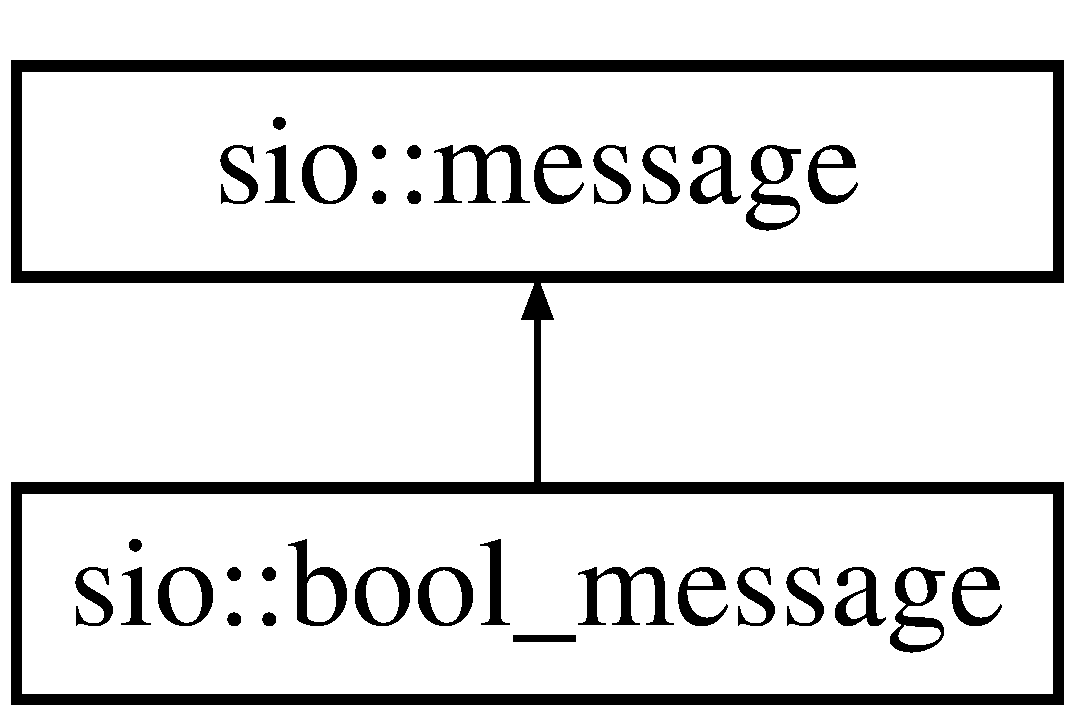
\includegraphics[height=2.000000cm]{classsio_1_1bool__message}
\end{center}
\end{figure}
\subsection*{Public Member Functions}
\begin{DoxyCompactItemize}
\item 
bool \hyperlink{classsio_1_1bool__message_aca66ff64b5ac4198c5292e26abdf9e92}{get\+\_\+bool} () const
\end{DoxyCompactItemize}
\subsection*{Static Public Member Functions}
\begin{DoxyCompactItemize}
\item 
static \hyperlink{classsio_1_1message_a6340b6fef57e4516eb17928b1885a615}{message\+::ptr} \hyperlink{classsio_1_1bool__message_a6742ca3443bd90ad25e3aa4ff5f20459}{create} (bool v)
\end{DoxyCompactItemize}
\subsection*{Protected Member Functions}
\begin{DoxyCompactItemize}
\item 
\hyperlink{classsio_1_1bool__message_a06e4eb255118501266a40d1ddcfd5d76}{bool\+\_\+message} (bool v)
\end{DoxyCompactItemize}
\subsection*{Additional Inherited Members}


\subsection{Constructor \& Destructor Documentation}
\mbox{\Hypertarget{classsio_1_1bool__message_a06e4eb255118501266a40d1ddcfd5d76}\label{classsio_1_1bool__message_a06e4eb255118501266a40d1ddcfd5d76}} 
\index{sio\+::bool\+\_\+message@{sio\+::bool\+\_\+message}!bool\+\_\+message@{bool\+\_\+message}}
\index{bool\+\_\+message@{bool\+\_\+message}!sio\+::bool\+\_\+message@{sio\+::bool\+\_\+message}}
\subsubsection{\texorpdfstring{bool\+\_\+message()}{bool\_message()}}
{\footnotesize\ttfamily sio\+::bool\+\_\+message\+::bool\+\_\+message (\begin{DoxyParamCaption}\item[{bool}]{v }\end{DoxyParamCaption})\hspace{0.3cm}{\ttfamily [inline]}, {\ttfamily [protected]}}



\subsection{Member Function Documentation}
\mbox{\Hypertarget{classsio_1_1bool__message_a6742ca3443bd90ad25e3aa4ff5f20459}\label{classsio_1_1bool__message_a6742ca3443bd90ad25e3aa4ff5f20459}} 
\index{sio\+::bool\+\_\+message@{sio\+::bool\+\_\+message}!create@{create}}
\index{create@{create}!sio\+::bool\+\_\+message@{sio\+::bool\+\_\+message}}
\subsubsection{\texorpdfstring{create()}{create()}}
{\footnotesize\ttfamily static \hyperlink{classsio_1_1message_a6340b6fef57e4516eb17928b1885a615}{message\+::ptr} sio\+::bool\+\_\+message\+::create (\begin{DoxyParamCaption}\item[{bool}]{v }\end{DoxyParamCaption})\hspace{0.3cm}{\ttfamily [inline]}, {\ttfamily [static]}}

\mbox{\Hypertarget{classsio_1_1bool__message_aca66ff64b5ac4198c5292e26abdf9e92}\label{classsio_1_1bool__message_aca66ff64b5ac4198c5292e26abdf9e92}} 
\index{sio\+::bool\+\_\+message@{sio\+::bool\+\_\+message}!get\+\_\+bool@{get\+\_\+bool}}
\index{get\+\_\+bool@{get\+\_\+bool}!sio\+::bool\+\_\+message@{sio\+::bool\+\_\+message}}
\subsubsection{\texorpdfstring{get\+\_\+bool()}{get\_bool()}}
{\footnotesize\ttfamily bool sio\+::bool\+\_\+message\+::get\+\_\+bool (\begin{DoxyParamCaption}{ }\end{DoxyParamCaption}) const\hspace{0.3cm}{\ttfamily [inline]}, {\ttfamily [virtual]}}



Reimplemented from \hyperlink{classsio_1_1message_a3acbec589c3dc214d44dd4db1a6f8a2c}{sio\+::message}.



The documentation for this class was generated from the following file\+:\begin{DoxyCompactItemize}
\item 
/home/erik/work/bridges/bridges-\/cxx/src/\hyperlink{sio__message_8h}{sio\+\_\+message.\+h}\end{DoxyCompactItemize}

\hypertarget{structbridges_1_1datastructure_1_1_array2_d_1_1_bracket__helper}{}\section{bridges\+::datastructure\+::Array2D$<$ E $>$\+::Bracket\+\_\+helper Struct Reference}
\label{structbridges_1_1datastructure_1_1_array2_d_1_1_bracket__helper}\index{bridges::datastructure::Array2D$<$ E $>$::Bracket\_helper@{bridges::datastructure::Array2D$<$ E $>$::Bracket\_helper}}


{\ttfamily \#include $<$Array2\+D.\+h$>$}



\subsection{Detailed Description}
\subsubsection*{template$<$typename E$>$\newline
struct bridges\+::datastructure\+::\+Array2\+D$<$ E $>$\+::\+Bracket\+\_\+helper}

helper class to make \mbox{[}\mbox{]}\mbox{[}\mbox{]} operators work on array 2d. You should never use it directly \subsection*{Public Member Functions}
\begin{DoxyCompactItemize}
\item 
\mbox{\hyperlink{structbridges_1_1datastructure_1_1_array2_d_1_1_bracket__helper_a483f18d5a65b80708598c2905b266edc}{Bracket\+\_\+helper}} (\mbox{\hyperlink{classbridges_1_1datastructure_1_1_array2_d}{Array2D}}$<$ E $>$ \&a, int r)
\item 
E \& \mbox{\hyperlink{structbridges_1_1datastructure_1_1_array2_d_1_1_bracket__helper_a799f5ce78138fddeeb1f91ac8b6bc247}{operator\mbox{[}$\,$\mbox{]}}} (int col)
\end{DoxyCompactItemize}
\subsection*{Public Attributes}
\begin{DoxyCompactItemize}
\item 
\mbox{\hyperlink{classbridges_1_1datastructure_1_1_array2_d}{Array2D}}$<$ E $>$ \& \mbox{\hyperlink{structbridges_1_1datastructure_1_1_array2_d_1_1_bracket__helper_a77fc2a11bc16c90eadfc0369c6f2979b}{arr}}
\item 
int \mbox{\hyperlink{structbridges_1_1datastructure_1_1_array2_d_1_1_bracket__helper_a6f09a65776d572d4fdfedb6c3a822e2a}{row}}
\end{DoxyCompactItemize}


\subsection{Constructor \& Destructor Documentation}
\mbox{\Hypertarget{structbridges_1_1datastructure_1_1_array2_d_1_1_bracket__helper_a483f18d5a65b80708598c2905b266edc}\label{structbridges_1_1datastructure_1_1_array2_d_1_1_bracket__helper_a483f18d5a65b80708598c2905b266edc}} 
\index{bridges::datastructure::Array2D$<$ E $>$::Bracket\_helper@{bridges::datastructure::Array2D$<$ E $>$::Bracket\_helper}!Bracket\_helper@{Bracket\_helper}}
\index{Bracket\_helper@{Bracket\_helper}!bridges::datastructure::Array2D$<$ E $>$::Bracket\_helper@{bridges::datastructure::Array2D$<$ E $>$::Bracket\_helper}}
\subsubsection{\texorpdfstring{Bracket\_helper()}{Bracket\_helper()}}
{\footnotesize\ttfamily template$<$typename E$>$ \\
\mbox{\hyperlink{classbridges_1_1datastructure_1_1_array2_d}{bridges\+::datastructure\+::\+Array2D}}$<$ E $>$\+::Bracket\+\_\+helper\+::\+Bracket\+\_\+helper (\begin{DoxyParamCaption}\item[{\mbox{\hyperlink{classbridges_1_1datastructure_1_1_array2_d}{Array2D}}$<$ E $>$ \&}]{a,  }\item[{int}]{r }\end{DoxyParamCaption})\hspace{0.3cm}{\ttfamily [inline]}}



\subsection{Member Function Documentation}
\mbox{\Hypertarget{structbridges_1_1datastructure_1_1_array2_d_1_1_bracket__helper_a799f5ce78138fddeeb1f91ac8b6bc247}\label{structbridges_1_1datastructure_1_1_array2_d_1_1_bracket__helper_a799f5ce78138fddeeb1f91ac8b6bc247}} 
\index{bridges::datastructure::Array2D$<$ E $>$::Bracket\_helper@{bridges::datastructure::Array2D$<$ E $>$::Bracket\_helper}!operator\mbox{[}\mbox{]}@{operator[]}}
\index{operator\mbox{[}\mbox{]}@{operator[]}!bridges::datastructure::Array2D$<$ E $>$::Bracket\_helper@{bridges::datastructure::Array2D$<$ E $>$::Bracket\_helper}}
\subsubsection{\texorpdfstring{operator[]()}{operator[]()}}
{\footnotesize\ttfamily template$<$typename E$>$ \\
E\& \mbox{\hyperlink{classbridges_1_1datastructure_1_1_array2_d}{bridges\+::datastructure\+::\+Array2D}}$<$ E $>$\+::Bracket\+\_\+helper\+::operator\mbox{[}$\,$\mbox{]} (\begin{DoxyParamCaption}\item[{int}]{col }\end{DoxyParamCaption})\hspace{0.3cm}{\ttfamily [inline]}}



\subsection{Member Data Documentation}
\mbox{\Hypertarget{structbridges_1_1datastructure_1_1_array2_d_1_1_bracket__helper_a77fc2a11bc16c90eadfc0369c6f2979b}\label{structbridges_1_1datastructure_1_1_array2_d_1_1_bracket__helper_a77fc2a11bc16c90eadfc0369c6f2979b}} 
\index{bridges::datastructure::Array2D$<$ E $>$::Bracket\_helper@{bridges::datastructure::Array2D$<$ E $>$::Bracket\_helper}!arr@{arr}}
\index{arr@{arr}!bridges::datastructure::Array2D$<$ E $>$::Bracket\_helper@{bridges::datastructure::Array2D$<$ E $>$::Bracket\_helper}}
\subsubsection{\texorpdfstring{arr}{arr}}
{\footnotesize\ttfamily template$<$typename E$>$ \\
\mbox{\hyperlink{classbridges_1_1datastructure_1_1_array2_d}{Array2D}}$<$E$>$\& \mbox{\hyperlink{classbridges_1_1datastructure_1_1_array2_d}{bridges\+::datastructure\+::\+Array2D}}$<$ E $>$\+::Bracket\+\_\+helper\+::arr}

\mbox{\Hypertarget{structbridges_1_1datastructure_1_1_array2_d_1_1_bracket__helper_a6f09a65776d572d4fdfedb6c3a822e2a}\label{structbridges_1_1datastructure_1_1_array2_d_1_1_bracket__helper_a6f09a65776d572d4fdfedb6c3a822e2a}} 
\index{bridges::datastructure::Array2D$<$ E $>$::Bracket\_helper@{bridges::datastructure::Array2D$<$ E $>$::Bracket\_helper}!row@{row}}
\index{row@{row}!bridges::datastructure::Array2D$<$ E $>$::Bracket\_helper@{bridges::datastructure::Array2D$<$ E $>$::Bracket\_helper}}
\subsubsection{\texorpdfstring{row}{row}}
{\footnotesize\ttfamily template$<$typename E$>$ \\
int \mbox{\hyperlink{classbridges_1_1datastructure_1_1_array2_d}{bridges\+::datastructure\+::\+Array2D}}$<$ E $>$\+::Bracket\+\_\+helper\+::row}



The documentation for this struct was generated from the following file\+:\begin{DoxyCompactItemize}
\item 
/\+Users/kalpathi/gr/bridges/cxx/src/\mbox{\hyperlink{_array2_d_8h}{Array2\+D.\+h}}\end{DoxyCompactItemize}

\hypertarget{structbridges_1_1datastructure_1_1_array3_d_1_1_bracket__helper}{}\section{bridges\+:\+:datastructure\+:\+:Array3D$<$ E $>$\+:\+:Bracket\+\_\+helper Struct Reference}
\label{structbridges_1_1datastructure_1_1_array3_d_1_1_bracket__helper}\index{bridges\+::datastructure\+::\+Array3\+D$<$ E $>$\+::\+Bracket\+\_\+helper@{bridges\+::datastructure\+::\+Array3\+D$<$ E $>$\+::\+Bracket\+\_\+helper}}


{\ttfamily \#include $<$Array3\+D.\+h$>$}



\subsection{Detailed Description}
\subsubsection*{template$<$typename E$>$\newline
struct bridges\+::datastructure\+::\+Array3\+D$<$ E $>$\+::\+Bracket\+\_\+helper}

helper class to make \mbox{[}\mbox{]}\mbox{[}\mbox{]} operators work on array 2d. You should never use it directly \subsection*{Public Member Functions}
\begin{DoxyCompactItemize}
\item 
\hyperlink{structbridges_1_1datastructure_1_1_array3_d_1_1_bracket__helper_a02888ffe46f3f1bfc8dda232bd2a3634}{Bracket\+\_\+helper} (\hyperlink{classbridges_1_1datastructure_1_1_array3_d}{Array3D}$<$ E $>$ \&a, int \hyperlink{structbridges_1_1datastructure_1_1_array3_d_1_1_bracket__helper_a66c392b3d6f3a326f632099c596d175c}{x})
\item 
\hyperlink{structbridges_1_1datastructure_1_1_array3_d_1_1_bracket__helper2}{Bracket\+\_\+helper2} \hyperlink{structbridges_1_1datastructure_1_1_array3_d_1_1_bracket__helper_ac5abb4226f77526ae2b77d96fd98f9fa}{operator\mbox{[}$\,$\mbox{]}} (int y)
\end{DoxyCompactItemize}
\subsection*{Public Attributes}
\begin{DoxyCompactItemize}
\item 
\hyperlink{classbridges_1_1datastructure_1_1_array3_d}{Array3D}$<$ E $>$ \& \hyperlink{structbridges_1_1datastructure_1_1_array3_d_1_1_bracket__helper_a103a7f1a8a32dd0109f9ef278407d49f}{arr}
\item 
int \hyperlink{structbridges_1_1datastructure_1_1_array3_d_1_1_bracket__helper_a66c392b3d6f3a326f632099c596d175c}{x}
\end{DoxyCompactItemize}


\subsection{Constructor \& Destructor Documentation}
\mbox{\Hypertarget{structbridges_1_1datastructure_1_1_array3_d_1_1_bracket__helper_a02888ffe46f3f1bfc8dda232bd2a3634}\label{structbridges_1_1datastructure_1_1_array3_d_1_1_bracket__helper_a02888ffe46f3f1bfc8dda232bd2a3634}} 
\index{bridges\+::datastructure\+::\+Array3\+D\+::\+Bracket\+\_\+helper@{bridges\+::datastructure\+::\+Array3\+D\+::\+Bracket\+\_\+helper}!Bracket\+\_\+helper@{Bracket\+\_\+helper}}
\index{Bracket\+\_\+helper@{Bracket\+\_\+helper}!bridges\+::datastructure\+::\+Array3\+D\+::\+Bracket\+\_\+helper@{bridges\+::datastructure\+::\+Array3\+D\+::\+Bracket\+\_\+helper}}
\subsubsection{\texorpdfstring{Bracket\+\_\+helper()}{Bracket\_helper()}}
{\footnotesize\ttfamily template$<$typename E$>$ \\
\hyperlink{classbridges_1_1datastructure_1_1_array3_d}{bridges\+::datastructure\+::\+Array3D}$<$ E $>$\+::Bracket\+\_\+helper\+::\+Bracket\+\_\+helper (\begin{DoxyParamCaption}\item[{\hyperlink{classbridges_1_1datastructure_1_1_array3_d}{Array3D}$<$ E $>$ \&}]{a,  }\item[{int}]{x }\end{DoxyParamCaption})\hspace{0.3cm}{\ttfamily [inline]}}



\subsection{Member Function Documentation}
\mbox{\Hypertarget{structbridges_1_1datastructure_1_1_array3_d_1_1_bracket__helper_ac5abb4226f77526ae2b77d96fd98f9fa}\label{structbridges_1_1datastructure_1_1_array3_d_1_1_bracket__helper_ac5abb4226f77526ae2b77d96fd98f9fa}} 
\index{bridges\+::datastructure\+::\+Array3\+D\+::\+Bracket\+\_\+helper@{bridges\+::datastructure\+::\+Array3\+D\+::\+Bracket\+\_\+helper}!operator\mbox{[}\mbox{]}@{operator[]}}
\index{operator\mbox{[}\mbox{]}@{operator[]}!bridges\+::datastructure\+::\+Array3\+D\+::\+Bracket\+\_\+helper@{bridges\+::datastructure\+::\+Array3\+D\+::\+Bracket\+\_\+helper}}
\subsubsection{\texorpdfstring{operator[]()}{operator[]()}}
{\footnotesize\ttfamily template$<$typename E$>$ \\
\hyperlink{structbridges_1_1datastructure_1_1_array3_d_1_1_bracket__helper2}{Bracket\+\_\+helper2} \hyperlink{classbridges_1_1datastructure_1_1_array3_d}{bridges\+::datastructure\+::\+Array3D}$<$ E $>$\+::Bracket\+\_\+helper\+::operator\mbox{[}$\,$\mbox{]} (\begin{DoxyParamCaption}\item[{int}]{y }\end{DoxyParamCaption})\hspace{0.3cm}{\ttfamily [inline]}}



\subsection{Member Data Documentation}
\mbox{\Hypertarget{structbridges_1_1datastructure_1_1_array3_d_1_1_bracket__helper_a103a7f1a8a32dd0109f9ef278407d49f}\label{structbridges_1_1datastructure_1_1_array3_d_1_1_bracket__helper_a103a7f1a8a32dd0109f9ef278407d49f}} 
\index{bridges\+::datastructure\+::\+Array3\+D\+::\+Bracket\+\_\+helper@{bridges\+::datastructure\+::\+Array3\+D\+::\+Bracket\+\_\+helper}!arr@{arr}}
\index{arr@{arr}!bridges\+::datastructure\+::\+Array3\+D\+::\+Bracket\+\_\+helper@{bridges\+::datastructure\+::\+Array3\+D\+::\+Bracket\+\_\+helper}}
\subsubsection{\texorpdfstring{arr}{arr}}
{\footnotesize\ttfamily template$<$typename E$>$ \\
\hyperlink{classbridges_1_1datastructure_1_1_array3_d}{Array3D}$<$E$>$\& \hyperlink{classbridges_1_1datastructure_1_1_array3_d}{bridges\+::datastructure\+::\+Array3D}$<$ E $>$\+::Bracket\+\_\+helper\+::arr}

\mbox{\Hypertarget{structbridges_1_1datastructure_1_1_array3_d_1_1_bracket__helper_a66c392b3d6f3a326f632099c596d175c}\label{structbridges_1_1datastructure_1_1_array3_d_1_1_bracket__helper_a66c392b3d6f3a326f632099c596d175c}} 
\index{bridges\+::datastructure\+::\+Array3\+D\+::\+Bracket\+\_\+helper@{bridges\+::datastructure\+::\+Array3\+D\+::\+Bracket\+\_\+helper}!x@{x}}
\index{x@{x}!bridges\+::datastructure\+::\+Array3\+D\+::\+Bracket\+\_\+helper@{bridges\+::datastructure\+::\+Array3\+D\+::\+Bracket\+\_\+helper}}
\subsubsection{\texorpdfstring{x}{x}}
{\footnotesize\ttfamily template$<$typename E$>$ \\
int \hyperlink{classbridges_1_1datastructure_1_1_array3_d}{bridges\+::datastructure\+::\+Array3D}$<$ E $>$\+::Bracket\+\_\+helper\+::x}



The documentation for this struct was generated from the following file\+:\begin{DoxyCompactItemize}
\item 
/home/erik/work/bridges/bridges-\/cxx/src/\hyperlink{_array3_d_8h}{Array3\+D.\+h}\end{DoxyCompactItemize}

\hypertarget{structbridges_1_1datastructure_1_1_array3_d_1_1_bracket__helper2}{}\section{bridges\+:\+:datastructure\+:\+:Array3D$<$ E $>$\+:\+:Bracket\+\_\+helper2 Struct Reference}
\label{structbridges_1_1datastructure_1_1_array3_d_1_1_bracket__helper2}\index{bridges\+::datastructure\+::\+Array3\+D$<$ E $>$\+::\+Bracket\+\_\+helper2@{bridges\+::datastructure\+::\+Array3\+D$<$ E $>$\+::\+Bracket\+\_\+helper2}}


{\ttfamily \#include $<$Array3\+D.\+h$>$}

\subsection*{Public Member Functions}
\begin{DoxyCompactItemize}
\item 
\mbox{\hyperlink{structbridges_1_1datastructure_1_1_array3_d_1_1_bracket__helper2_ac6d8b305dcacc2b1b6d314f2697f78d7}{Bracket\+\_\+helper2}} (\mbox{\hyperlink{classbridges_1_1datastructure_1_1_array3_d}{Array3D}}$<$ E $>$ \&a, int \mbox{\hyperlink{structbridges_1_1datastructure_1_1_array3_d_1_1_bracket__helper2_acd07b57146e72a86ff87e6a00025549a}{x}}, int \mbox{\hyperlink{structbridges_1_1datastructure_1_1_array3_d_1_1_bracket__helper2_a2bd3e3e4253b14e14f1803b49d2f6dca}{y}})
\item 
E \& \mbox{\hyperlink{structbridges_1_1datastructure_1_1_array3_d_1_1_bracket__helper2_a7e8434ee60b6c04571db79bde1b555a4}{operator\mbox{[}$\,$\mbox{]}}} (int z)
\end{DoxyCompactItemize}
\subsection*{Public Attributes}
\begin{DoxyCompactItemize}
\item 
\mbox{\hyperlink{classbridges_1_1datastructure_1_1_array3_d}{Array3D}}$<$ E $>$ \& \mbox{\hyperlink{structbridges_1_1datastructure_1_1_array3_d_1_1_bracket__helper2_a72b1c40a7436cb6f9488ce2fc163ff83}{arr}}
\item 
int \mbox{\hyperlink{structbridges_1_1datastructure_1_1_array3_d_1_1_bracket__helper2_acd07b57146e72a86ff87e6a00025549a}{x}}
\item 
int \mbox{\hyperlink{structbridges_1_1datastructure_1_1_array3_d_1_1_bracket__helper2_a2bd3e3e4253b14e14f1803b49d2f6dca}{y}}
\end{DoxyCompactItemize}


\subsection{Constructor \& Destructor Documentation}
\mbox{\Hypertarget{structbridges_1_1datastructure_1_1_array3_d_1_1_bracket__helper2_ac6d8b305dcacc2b1b6d314f2697f78d7}\label{structbridges_1_1datastructure_1_1_array3_d_1_1_bracket__helper2_ac6d8b305dcacc2b1b6d314f2697f78d7}} 
\index{bridges\+::datastructure\+::\+Array3\+D\+::\+Bracket\+\_\+helper2@{bridges\+::datastructure\+::\+Array3\+D\+::\+Bracket\+\_\+helper2}!Bracket\+\_\+helper2@{Bracket\+\_\+helper2}}
\index{Bracket\+\_\+helper2@{Bracket\+\_\+helper2}!bridges\+::datastructure\+::\+Array3\+D\+::\+Bracket\+\_\+helper2@{bridges\+::datastructure\+::\+Array3\+D\+::\+Bracket\+\_\+helper2}}
\subsubsection{\texorpdfstring{Bracket\+\_\+helper2()}{Bracket\_helper2()}}
{\footnotesize\ttfamily template$<$typename E$>$ \\
\mbox{\hyperlink{classbridges_1_1datastructure_1_1_array3_d}{bridges\+::datastructure\+::\+Array3D}}$<$ E $>$\+::Bracket\+\_\+helper2\+::\+Bracket\+\_\+helper2 (\begin{DoxyParamCaption}\item[{\mbox{\hyperlink{classbridges_1_1datastructure_1_1_array3_d}{Array3D}}$<$ E $>$ \&}]{a,  }\item[{int}]{x,  }\item[{int}]{y }\end{DoxyParamCaption})\hspace{0.3cm}{\ttfamily [inline]}}



\subsection{Member Function Documentation}
\mbox{\Hypertarget{structbridges_1_1datastructure_1_1_array3_d_1_1_bracket__helper2_a7e8434ee60b6c04571db79bde1b555a4}\label{structbridges_1_1datastructure_1_1_array3_d_1_1_bracket__helper2_a7e8434ee60b6c04571db79bde1b555a4}} 
\index{bridges\+::datastructure\+::\+Array3\+D\+::\+Bracket\+\_\+helper2@{bridges\+::datastructure\+::\+Array3\+D\+::\+Bracket\+\_\+helper2}!operator\mbox{[}\mbox{]}@{operator[]}}
\index{operator\mbox{[}\mbox{]}@{operator[]}!bridges\+::datastructure\+::\+Array3\+D\+::\+Bracket\+\_\+helper2@{bridges\+::datastructure\+::\+Array3\+D\+::\+Bracket\+\_\+helper2}}
\subsubsection{\texorpdfstring{operator[]()}{operator[]()}}
{\footnotesize\ttfamily template$<$typename E$>$ \\
E\& \mbox{\hyperlink{classbridges_1_1datastructure_1_1_array3_d}{bridges\+::datastructure\+::\+Array3D}}$<$ E $>$\+::Bracket\+\_\+helper2\+::operator\mbox{[}$\,$\mbox{]} (\begin{DoxyParamCaption}\item[{int}]{z }\end{DoxyParamCaption})\hspace{0.3cm}{\ttfamily [inline]}}



\subsection{Member Data Documentation}
\mbox{\Hypertarget{structbridges_1_1datastructure_1_1_array3_d_1_1_bracket__helper2_a72b1c40a7436cb6f9488ce2fc163ff83}\label{structbridges_1_1datastructure_1_1_array3_d_1_1_bracket__helper2_a72b1c40a7436cb6f9488ce2fc163ff83}} 
\index{bridges\+::datastructure\+::\+Array3\+D\+::\+Bracket\+\_\+helper2@{bridges\+::datastructure\+::\+Array3\+D\+::\+Bracket\+\_\+helper2}!arr@{arr}}
\index{arr@{arr}!bridges\+::datastructure\+::\+Array3\+D\+::\+Bracket\+\_\+helper2@{bridges\+::datastructure\+::\+Array3\+D\+::\+Bracket\+\_\+helper2}}
\subsubsection{\texorpdfstring{arr}{arr}}
{\footnotesize\ttfamily template$<$typename E$>$ \\
\mbox{\hyperlink{classbridges_1_1datastructure_1_1_array3_d}{Array3D}}$<$E$>$\& \mbox{\hyperlink{classbridges_1_1datastructure_1_1_array3_d}{bridges\+::datastructure\+::\+Array3D}}$<$ E $>$\+::Bracket\+\_\+helper2\+::arr}

\mbox{\Hypertarget{structbridges_1_1datastructure_1_1_array3_d_1_1_bracket__helper2_acd07b57146e72a86ff87e6a00025549a}\label{structbridges_1_1datastructure_1_1_array3_d_1_1_bracket__helper2_acd07b57146e72a86ff87e6a00025549a}} 
\index{bridges\+::datastructure\+::\+Array3\+D\+::\+Bracket\+\_\+helper2@{bridges\+::datastructure\+::\+Array3\+D\+::\+Bracket\+\_\+helper2}!x@{x}}
\index{x@{x}!bridges\+::datastructure\+::\+Array3\+D\+::\+Bracket\+\_\+helper2@{bridges\+::datastructure\+::\+Array3\+D\+::\+Bracket\+\_\+helper2}}
\subsubsection{\texorpdfstring{x}{x}}
{\footnotesize\ttfamily template$<$typename E$>$ \\
int \mbox{\hyperlink{classbridges_1_1datastructure_1_1_array3_d}{bridges\+::datastructure\+::\+Array3D}}$<$ E $>$\+::Bracket\+\_\+helper2\+::x}

\mbox{\Hypertarget{structbridges_1_1datastructure_1_1_array3_d_1_1_bracket__helper2_a2bd3e3e4253b14e14f1803b49d2f6dca}\label{structbridges_1_1datastructure_1_1_array3_d_1_1_bracket__helper2_a2bd3e3e4253b14e14f1803b49d2f6dca}} 
\index{bridges\+::datastructure\+::\+Array3\+D\+::\+Bracket\+\_\+helper2@{bridges\+::datastructure\+::\+Array3\+D\+::\+Bracket\+\_\+helper2}!y@{y}}
\index{y@{y}!bridges\+::datastructure\+::\+Array3\+D\+::\+Bracket\+\_\+helper2@{bridges\+::datastructure\+::\+Array3\+D\+::\+Bracket\+\_\+helper2}}
\subsubsection{\texorpdfstring{y}{y}}
{\footnotesize\ttfamily template$<$typename E$>$ \\
int \mbox{\hyperlink{classbridges_1_1datastructure_1_1_array3_d}{bridges\+::datastructure\+::\+Array3D}}$<$ E $>$\+::Bracket\+\_\+helper2\+::y}



The documentation for this struct was generated from the following file\+:\begin{DoxyCompactItemize}
\item 
/\+Users/kalpathi/gr/bridges/client/cxx/src/\mbox{\hyperlink{_array3_d_8h}{Array3\+D.\+h}}\end{DoxyCompactItemize}

\hypertarget{structbridges_1_1datastructure_1_1_array3_d_1_1_bracket__helper2__const}{}\doxysection{bridges\+::datastructure\+::Array3D$<$ E $>$\+::Bracket\+\_\+helper2\+\_\+const Struct Reference}
\label{structbridges_1_1datastructure_1_1_array3_d_1_1_bracket__helper2__const}\index{bridges::datastructure::Array3D$<$ E $>$::Bracket\_helper2\_const@{bridges::datastructure::Array3D$<$ E $>$::Bracket\_helper2\_const}}


{\ttfamily \#include $<$Array3\+D.\+h$>$}



\doxysubsection{Detailed Description}
\subsubsection*{template$<$typename E$>$\newline
struct bridges\+::datastructure\+::\+Array3\+D$<$ E $>$\+::\+Bracket\+\_\+helper2\+\_\+const}

helper2 const class is to make \mbox{[}\mbox{]}\mbox{[}\mbox{]} operators work on array 2d. You should never use it directly \doxysubsection*{Public Member Functions}
\begin{DoxyCompactItemize}
\item 
\mbox{\hyperlink{structbridges_1_1datastructure_1_1_array3_d_1_1_bracket__helper2__const_a30128c8c2025bb03325b2c91020dabc5}{Bracket\+\_\+helper2\+\_\+const}} (\mbox{\hyperlink{classbridges_1_1datastructure_1_1_array3_d}{Array3D}}$<$ E $>$ \&a, int \mbox{\hyperlink{structbridges_1_1datastructure_1_1_array3_d_1_1_bracket__helper2__const_af71fd602aef4eac98d6ffe3f13f42dd8}{x}}, int \mbox{\hyperlink{structbridges_1_1datastructure_1_1_array3_d_1_1_bracket__helper2__const_a5c76d396209c5060f72c321d2b70e707}{y}})
\item 
E const  \& \mbox{\hyperlink{structbridges_1_1datastructure_1_1_array3_d_1_1_bracket__helper2__const_a55b6db54acf32062d3dbba7ce72e643f}{operator\mbox{[}$\,$\mbox{]}}} (int z) const
\end{DoxyCompactItemize}
\doxysubsection*{Public Attributes}
\begin{DoxyCompactItemize}
\item 
\mbox{\hyperlink{classbridges_1_1datastructure_1_1_array3_d}{Array3D}}$<$ E $>$ const  \& \mbox{\hyperlink{structbridges_1_1datastructure_1_1_array3_d_1_1_bracket__helper2__const_a61e67ef891a27c8c45dd7f0c60dfdad4}{arr}}
\item 
int \mbox{\hyperlink{structbridges_1_1datastructure_1_1_array3_d_1_1_bracket__helper2__const_af71fd602aef4eac98d6ffe3f13f42dd8}{x}}
\item 
int \mbox{\hyperlink{structbridges_1_1datastructure_1_1_array3_d_1_1_bracket__helper2__const_a5c76d396209c5060f72c321d2b70e707}{y}}
\end{DoxyCompactItemize}


\doxysubsection{Constructor \& Destructor Documentation}
\mbox{\Hypertarget{structbridges_1_1datastructure_1_1_array3_d_1_1_bracket__helper2__const_a30128c8c2025bb03325b2c91020dabc5}\label{structbridges_1_1datastructure_1_1_array3_d_1_1_bracket__helper2__const_a30128c8c2025bb03325b2c91020dabc5}} 
\index{bridges::datastructure::Array3D$<$ E $>$::Bracket\_helper2\_const@{bridges::datastructure::Array3D$<$ E $>$::Bracket\_helper2\_const}!Bracket\_helper2\_const@{Bracket\_helper2\_const}}
\index{Bracket\_helper2\_const@{Bracket\_helper2\_const}!bridges::datastructure::Array3D$<$ E $>$::Bracket\_helper2\_const@{bridges::datastructure::Array3D$<$ E $>$::Bracket\_helper2\_const}}
\doxysubsubsection{\texorpdfstring{Bracket\_helper2\_const()}{Bracket\_helper2\_const()}}
{\footnotesize\ttfamily template$<$typename E $>$ \\
\mbox{\hyperlink{classbridges_1_1datastructure_1_1_array3_d}{bridges\+::datastructure\+::\+Array3D}}$<$ E $>$\+::Bracket\+\_\+helper2\+\_\+const\+::\+Bracket\+\_\+helper2\+\_\+const (\begin{DoxyParamCaption}\item[{\mbox{\hyperlink{classbridges_1_1datastructure_1_1_array3_d}{Array3D}}$<$ E $>$ \&}]{a,  }\item[{int}]{x,  }\item[{int}]{y }\end{DoxyParamCaption})\hspace{0.3cm}{\ttfamily [inline]}}



\doxysubsection{Member Function Documentation}
\mbox{\Hypertarget{structbridges_1_1datastructure_1_1_array3_d_1_1_bracket__helper2__const_a55b6db54acf32062d3dbba7ce72e643f}\label{structbridges_1_1datastructure_1_1_array3_d_1_1_bracket__helper2__const_a55b6db54acf32062d3dbba7ce72e643f}} 
\index{bridges::datastructure::Array3D$<$ E $>$::Bracket\_helper2\_const@{bridges::datastructure::Array3D$<$ E $>$::Bracket\_helper2\_const}!operator\mbox{[}\mbox{]}@{operator[]}}
\index{operator\mbox{[}\mbox{]}@{operator[]}!bridges::datastructure::Array3D$<$ E $>$::Bracket\_helper2\_const@{bridges::datastructure::Array3D$<$ E $>$::Bracket\_helper2\_const}}
\doxysubsubsection{\texorpdfstring{operator[]()}{operator[]()}}
{\footnotesize\ttfamily template$<$typename E $>$ \\
E const\& \mbox{\hyperlink{classbridges_1_1datastructure_1_1_array3_d}{bridges\+::datastructure\+::\+Array3D}}$<$ E $>$\+::Bracket\+\_\+helper2\+\_\+const\+::operator\mbox{[}$\,$\mbox{]} (\begin{DoxyParamCaption}\item[{int}]{z }\end{DoxyParamCaption}) const\hspace{0.3cm}{\ttfamily [inline]}}



\doxysubsection{Member Data Documentation}
\mbox{\Hypertarget{structbridges_1_1datastructure_1_1_array3_d_1_1_bracket__helper2__const_a61e67ef891a27c8c45dd7f0c60dfdad4}\label{structbridges_1_1datastructure_1_1_array3_d_1_1_bracket__helper2__const_a61e67ef891a27c8c45dd7f0c60dfdad4}} 
\index{bridges::datastructure::Array3D$<$ E $>$::Bracket\_helper2\_const@{bridges::datastructure::Array3D$<$ E $>$::Bracket\_helper2\_const}!arr@{arr}}
\index{arr@{arr}!bridges::datastructure::Array3D$<$ E $>$::Bracket\_helper2\_const@{bridges::datastructure::Array3D$<$ E $>$::Bracket\_helper2\_const}}
\doxysubsubsection{\texorpdfstring{arr}{arr}}
{\footnotesize\ttfamily template$<$typename E $>$ \\
\mbox{\hyperlink{classbridges_1_1datastructure_1_1_array3_d}{Array3D}}$<$E$>$ const\& \mbox{\hyperlink{classbridges_1_1datastructure_1_1_array3_d}{bridges\+::datastructure\+::\+Array3D}}$<$ E $>$\+::Bracket\+\_\+helper2\+\_\+const\+::arr}

\mbox{\Hypertarget{structbridges_1_1datastructure_1_1_array3_d_1_1_bracket__helper2__const_af71fd602aef4eac98d6ffe3f13f42dd8}\label{structbridges_1_1datastructure_1_1_array3_d_1_1_bracket__helper2__const_af71fd602aef4eac98d6ffe3f13f42dd8}} 
\index{bridges::datastructure::Array3D$<$ E $>$::Bracket\_helper2\_const@{bridges::datastructure::Array3D$<$ E $>$::Bracket\_helper2\_const}!x@{x}}
\index{x@{x}!bridges::datastructure::Array3D$<$ E $>$::Bracket\_helper2\_const@{bridges::datastructure::Array3D$<$ E $>$::Bracket\_helper2\_const}}
\doxysubsubsection{\texorpdfstring{x}{x}}
{\footnotesize\ttfamily template$<$typename E $>$ \\
int \mbox{\hyperlink{classbridges_1_1datastructure_1_1_array3_d}{bridges\+::datastructure\+::\+Array3D}}$<$ E $>$\+::Bracket\+\_\+helper2\+\_\+const\+::x}

\mbox{\Hypertarget{structbridges_1_1datastructure_1_1_array3_d_1_1_bracket__helper2__const_a5c76d396209c5060f72c321d2b70e707}\label{structbridges_1_1datastructure_1_1_array3_d_1_1_bracket__helper2__const_a5c76d396209c5060f72c321d2b70e707}} 
\index{bridges::datastructure::Array3D$<$ E $>$::Bracket\_helper2\_const@{bridges::datastructure::Array3D$<$ E $>$::Bracket\_helper2\_const}!y@{y}}
\index{y@{y}!bridges::datastructure::Array3D$<$ E $>$::Bracket\_helper2\_const@{bridges::datastructure::Array3D$<$ E $>$::Bracket\_helper2\_const}}
\doxysubsubsection{\texorpdfstring{y}{y}}
{\footnotesize\ttfamily template$<$typename E $>$ \\
int \mbox{\hyperlink{classbridges_1_1datastructure_1_1_array3_d}{bridges\+::datastructure\+::\+Array3D}}$<$ E $>$\+::Bracket\+\_\+helper2\+\_\+const\+::y}



The documentation for this struct was generated from the following file\+:\begin{DoxyCompactItemize}
\item 
/home/erik/work/bridges/bridges-\/cxx/src/\mbox{\hyperlink{_array3_d_8h}{Array3\+D.\+h}}\end{DoxyCompactItemize}

\hypertarget{structbridges_1_1datastructure_1_1_array2_d_1_1_bracket__helper__const}{}\doxysection{bridges\+::datastructure\+::Array2D$<$ E $>$\+::Bracket\+\_\+helper\+\_\+const Struct Reference}
\label{structbridges_1_1datastructure_1_1_array2_d_1_1_bracket__helper__const}\index{bridges::datastructure::Array2D$<$ E $>$::Bracket\_helper\_const@{bridges::datastructure::Array2D$<$ E $>$::Bracket\_helper\_const}}


{\ttfamily \#include $<$Array2\+D.\+h$>$}



\doxysubsection{Detailed Description}
\subsubsection*{template$<$typename E$>$\newline
struct bridges\+::datastructure\+::\+Array2\+D$<$ E $>$\+::\+Bracket\+\_\+helper\+\_\+const}

helper class to make \mbox{[}\mbox{]}\mbox{[}\mbox{]} operators work on array 2d. You should never use it directly \doxysubsection*{Public Member Functions}
\begin{DoxyCompactItemize}
\item 
\mbox{\hyperlink{structbridges_1_1datastructure_1_1_array2_d_1_1_bracket__helper__const_a6025129e8bb49c03d6f724829b6a7620}{Bracket\+\_\+helper\+\_\+const}} (\mbox{\hyperlink{classbridges_1_1datastructure_1_1_array2_d}{Array2D}}$<$ E $>$ \&a, int r)
\item 
E const  \& \mbox{\hyperlink{structbridges_1_1datastructure_1_1_array2_d_1_1_bracket__helper__const_a2422c26669a313801f7ebfe6e6f46c47}{operator\mbox{[}$\,$\mbox{]}}} (int col) const
\end{DoxyCompactItemize}
\doxysubsection*{Public Attributes}
\begin{DoxyCompactItemize}
\item 
\mbox{\hyperlink{classbridges_1_1datastructure_1_1_array2_d}{Array2D}}$<$ E $>$ const  \& \mbox{\hyperlink{structbridges_1_1datastructure_1_1_array2_d_1_1_bracket__helper__const_a3aecc3cdd163aad0a6dfac6ff1379f1c}{arr}}
\item 
int \mbox{\hyperlink{structbridges_1_1datastructure_1_1_array2_d_1_1_bracket__helper__const_a1c82a30f3c342a90c009abb400b5557d}{row}}
\end{DoxyCompactItemize}


\doxysubsection{Constructor \& Destructor Documentation}
\mbox{\Hypertarget{structbridges_1_1datastructure_1_1_array2_d_1_1_bracket__helper__const_a6025129e8bb49c03d6f724829b6a7620}\label{structbridges_1_1datastructure_1_1_array2_d_1_1_bracket__helper__const_a6025129e8bb49c03d6f724829b6a7620}} 
\index{bridges::datastructure::Array2D$<$ E $>$::Bracket\_helper\_const@{bridges::datastructure::Array2D$<$ E $>$::Bracket\_helper\_const}!Bracket\_helper\_const@{Bracket\_helper\_const}}
\index{Bracket\_helper\_const@{Bracket\_helper\_const}!bridges::datastructure::Array2D$<$ E $>$::Bracket\_helper\_const@{bridges::datastructure::Array2D$<$ E $>$::Bracket\_helper\_const}}
\doxysubsubsection{\texorpdfstring{Bracket\_helper\_const()}{Bracket\_helper\_const()}}
{\footnotesize\ttfamily template$<$typename E $>$ \\
\mbox{\hyperlink{classbridges_1_1datastructure_1_1_array2_d}{bridges\+::datastructure\+::\+Array2D}}$<$ E $>$\+::Bracket\+\_\+helper\+\_\+const\+::\+Bracket\+\_\+helper\+\_\+const (\begin{DoxyParamCaption}\item[{\mbox{\hyperlink{classbridges_1_1datastructure_1_1_array2_d}{Array2D}}$<$ E $>$ \&}]{a,  }\item[{int}]{r }\end{DoxyParamCaption})\hspace{0.3cm}{\ttfamily [inline]}}



\doxysubsection{Member Function Documentation}
\mbox{\Hypertarget{structbridges_1_1datastructure_1_1_array2_d_1_1_bracket__helper__const_a2422c26669a313801f7ebfe6e6f46c47}\label{structbridges_1_1datastructure_1_1_array2_d_1_1_bracket__helper__const_a2422c26669a313801f7ebfe6e6f46c47}} 
\index{bridges::datastructure::Array2D$<$ E $>$::Bracket\_helper\_const@{bridges::datastructure::Array2D$<$ E $>$::Bracket\_helper\_const}!operator\mbox{[}\mbox{]}@{operator[]}}
\index{operator\mbox{[}\mbox{]}@{operator[]}!bridges::datastructure::Array2D$<$ E $>$::Bracket\_helper\_const@{bridges::datastructure::Array2D$<$ E $>$::Bracket\_helper\_const}}
\doxysubsubsection{\texorpdfstring{operator[]()}{operator[]()}}
{\footnotesize\ttfamily template$<$typename E $>$ \\
E const\& \mbox{\hyperlink{classbridges_1_1datastructure_1_1_array2_d}{bridges\+::datastructure\+::\+Array2D}}$<$ E $>$\+::Bracket\+\_\+helper\+\_\+const\+::operator\mbox{[}$\,$\mbox{]} (\begin{DoxyParamCaption}\item[{int}]{col }\end{DoxyParamCaption}) const\hspace{0.3cm}{\ttfamily [inline]}}



\doxysubsection{Member Data Documentation}
\mbox{\Hypertarget{structbridges_1_1datastructure_1_1_array2_d_1_1_bracket__helper__const_a3aecc3cdd163aad0a6dfac6ff1379f1c}\label{structbridges_1_1datastructure_1_1_array2_d_1_1_bracket__helper__const_a3aecc3cdd163aad0a6dfac6ff1379f1c}} 
\index{bridges::datastructure::Array2D$<$ E $>$::Bracket\_helper\_const@{bridges::datastructure::Array2D$<$ E $>$::Bracket\_helper\_const}!arr@{arr}}
\index{arr@{arr}!bridges::datastructure::Array2D$<$ E $>$::Bracket\_helper\_const@{bridges::datastructure::Array2D$<$ E $>$::Bracket\_helper\_const}}
\doxysubsubsection{\texorpdfstring{arr}{arr}}
{\footnotesize\ttfamily template$<$typename E $>$ \\
\mbox{\hyperlink{classbridges_1_1datastructure_1_1_array2_d}{Array2D}}$<$E$>$ const\& \mbox{\hyperlink{classbridges_1_1datastructure_1_1_array2_d}{bridges\+::datastructure\+::\+Array2D}}$<$ E $>$\+::Bracket\+\_\+helper\+\_\+const\+::arr}

\mbox{\Hypertarget{structbridges_1_1datastructure_1_1_array2_d_1_1_bracket__helper__const_a1c82a30f3c342a90c009abb400b5557d}\label{structbridges_1_1datastructure_1_1_array2_d_1_1_bracket__helper__const_a1c82a30f3c342a90c009abb400b5557d}} 
\index{bridges::datastructure::Array2D$<$ E $>$::Bracket\_helper\_const@{bridges::datastructure::Array2D$<$ E $>$::Bracket\_helper\_const}!row@{row}}
\index{row@{row}!bridges::datastructure::Array2D$<$ E $>$::Bracket\_helper\_const@{bridges::datastructure::Array2D$<$ E $>$::Bracket\_helper\_const}}
\doxysubsubsection{\texorpdfstring{row}{row}}
{\footnotesize\ttfamily template$<$typename E $>$ \\
int \mbox{\hyperlink{classbridges_1_1datastructure_1_1_array2_d}{bridges\+::datastructure\+::\+Array2D}}$<$ E $>$\+::Bracket\+\_\+helper\+\_\+const\+::row}



The documentation for this struct was generated from the following file\+:\begin{DoxyCompactItemize}
\item 
/home/erik/work/bridges/bridges-\/cxx/src/\mbox{\hyperlink{_array2_d_8h}{Array2\+D.\+h}}\end{DoxyCompactItemize}

\hypertarget{structbridges_1_1datastructure_1_1_array3_d_1_1_bracket__helper__const}{}\section{bridges\+:\+:datastructure\+:\+:Array3D$<$ E $>$\+:\+:Bracket\+\_\+helper\+\_\+const Struct Reference}
\label{structbridges_1_1datastructure_1_1_array3_d_1_1_bracket__helper__const}\index{bridges\+::datastructure\+::\+Array3\+D$<$ E $>$\+::\+Bracket\+\_\+helper\+\_\+const@{bridges\+::datastructure\+::\+Array3\+D$<$ E $>$\+::\+Bracket\+\_\+helper\+\_\+const}}


{\ttfamily \#include $<$Array3\+D.\+h$>$}



\subsection{Detailed Description}
\subsubsection*{template$<$typename E$>$\newline
struct bridges\+::datastructure\+::\+Array3\+D$<$ E $>$\+::\+Bracket\+\_\+helper\+\_\+const}

helper class to make \mbox{[}\mbox{]}\mbox{[}\mbox{]} operators work on array 2d. You should never use it directly \subsection*{Public Member Functions}
\begin{DoxyCompactItemize}
\item 
\hyperlink{structbridges_1_1datastructure_1_1_array3_d_1_1_bracket__helper__const_a9b87bdb88f75416d5953efe779586856}{Bracket\+\_\+helper\+\_\+const} (\hyperlink{classbridges_1_1datastructure_1_1_array3_d}{Array3D}$<$ E $>$ \&a, int \hyperlink{structbridges_1_1datastructure_1_1_array3_d_1_1_bracket__helper__const_ae7538519eb75fa07fbd06ab9754b6727}{x})
\item 
\hyperlink{structbridges_1_1datastructure_1_1_array3_d_1_1_bracket__helper2__const}{Bracket\+\_\+helper2\+\_\+const} \hyperlink{structbridges_1_1datastructure_1_1_array3_d_1_1_bracket__helper__const_a952373a0e03a47f3d588462d830efdb4}{operator\mbox{[}$\,$\mbox{]}} (int y) const
\end{DoxyCompactItemize}
\subsection*{Public Attributes}
\begin{DoxyCompactItemize}
\item 
\hyperlink{classbridges_1_1datastructure_1_1_array3_d}{Array3D}$<$ E $>$ const  \& \hyperlink{structbridges_1_1datastructure_1_1_array3_d_1_1_bracket__helper__const_afb5d187eb87a722b9e2e67f72891d01c}{arr}
\item 
int \hyperlink{structbridges_1_1datastructure_1_1_array3_d_1_1_bracket__helper__const_ae7538519eb75fa07fbd06ab9754b6727}{x}
\end{DoxyCompactItemize}


\subsection{Constructor \& Destructor Documentation}
\mbox{\Hypertarget{structbridges_1_1datastructure_1_1_array3_d_1_1_bracket__helper__const_a9b87bdb88f75416d5953efe779586856}\label{structbridges_1_1datastructure_1_1_array3_d_1_1_bracket__helper__const_a9b87bdb88f75416d5953efe779586856}} 
\index{bridges\+::datastructure\+::\+Array3\+D\+::\+Bracket\+\_\+helper\+\_\+const@{bridges\+::datastructure\+::\+Array3\+D\+::\+Bracket\+\_\+helper\+\_\+const}!Bracket\+\_\+helper\+\_\+const@{Bracket\+\_\+helper\+\_\+const}}
\index{Bracket\+\_\+helper\+\_\+const@{Bracket\+\_\+helper\+\_\+const}!bridges\+::datastructure\+::\+Array3\+D\+::\+Bracket\+\_\+helper\+\_\+const@{bridges\+::datastructure\+::\+Array3\+D\+::\+Bracket\+\_\+helper\+\_\+const}}
\subsubsection{\texorpdfstring{Bracket\+\_\+helper\+\_\+const()}{Bracket\_helper\_const()}}
{\footnotesize\ttfamily template$<$typename E$>$ \\
\hyperlink{classbridges_1_1datastructure_1_1_array3_d}{bridges\+::datastructure\+::\+Array3D}$<$ E $>$\+::Bracket\+\_\+helper\+\_\+const\+::\+Bracket\+\_\+helper\+\_\+const (\begin{DoxyParamCaption}\item[{\hyperlink{classbridges_1_1datastructure_1_1_array3_d}{Array3D}$<$ E $>$ \&}]{a,  }\item[{int}]{x }\end{DoxyParamCaption})\hspace{0.3cm}{\ttfamily [inline]}}



\subsection{Member Function Documentation}
\mbox{\Hypertarget{structbridges_1_1datastructure_1_1_array3_d_1_1_bracket__helper__const_a952373a0e03a47f3d588462d830efdb4}\label{structbridges_1_1datastructure_1_1_array3_d_1_1_bracket__helper__const_a952373a0e03a47f3d588462d830efdb4}} 
\index{bridges\+::datastructure\+::\+Array3\+D\+::\+Bracket\+\_\+helper\+\_\+const@{bridges\+::datastructure\+::\+Array3\+D\+::\+Bracket\+\_\+helper\+\_\+const}!operator\mbox{[}\mbox{]}@{operator[]}}
\index{operator\mbox{[}\mbox{]}@{operator[]}!bridges\+::datastructure\+::\+Array3\+D\+::\+Bracket\+\_\+helper\+\_\+const@{bridges\+::datastructure\+::\+Array3\+D\+::\+Bracket\+\_\+helper\+\_\+const}}
\subsubsection{\texorpdfstring{operator[]()}{operator[]()}}
{\footnotesize\ttfamily template$<$typename E$>$ \\
\hyperlink{structbridges_1_1datastructure_1_1_array3_d_1_1_bracket__helper2__const}{Bracket\+\_\+helper2\+\_\+const} \hyperlink{classbridges_1_1datastructure_1_1_array3_d}{bridges\+::datastructure\+::\+Array3D}$<$ E $>$\+::Bracket\+\_\+helper\+\_\+const\+::operator\mbox{[}$\,$\mbox{]} (\begin{DoxyParamCaption}\item[{int}]{y }\end{DoxyParamCaption}) const\hspace{0.3cm}{\ttfamily [inline]}}



\subsection{Member Data Documentation}
\mbox{\Hypertarget{structbridges_1_1datastructure_1_1_array3_d_1_1_bracket__helper__const_afb5d187eb87a722b9e2e67f72891d01c}\label{structbridges_1_1datastructure_1_1_array3_d_1_1_bracket__helper__const_afb5d187eb87a722b9e2e67f72891d01c}} 
\index{bridges\+::datastructure\+::\+Array3\+D\+::\+Bracket\+\_\+helper\+\_\+const@{bridges\+::datastructure\+::\+Array3\+D\+::\+Bracket\+\_\+helper\+\_\+const}!arr@{arr}}
\index{arr@{arr}!bridges\+::datastructure\+::\+Array3\+D\+::\+Bracket\+\_\+helper\+\_\+const@{bridges\+::datastructure\+::\+Array3\+D\+::\+Bracket\+\_\+helper\+\_\+const}}
\subsubsection{\texorpdfstring{arr}{arr}}
{\footnotesize\ttfamily template$<$typename E$>$ \\
\hyperlink{classbridges_1_1datastructure_1_1_array3_d}{Array3D}$<$E$>$ const\& \hyperlink{classbridges_1_1datastructure_1_1_array3_d}{bridges\+::datastructure\+::\+Array3D}$<$ E $>$\+::Bracket\+\_\+helper\+\_\+const\+::arr}

\mbox{\Hypertarget{structbridges_1_1datastructure_1_1_array3_d_1_1_bracket__helper__const_ae7538519eb75fa07fbd06ab9754b6727}\label{structbridges_1_1datastructure_1_1_array3_d_1_1_bracket__helper__const_ae7538519eb75fa07fbd06ab9754b6727}} 
\index{bridges\+::datastructure\+::\+Array3\+D\+::\+Bracket\+\_\+helper\+\_\+const@{bridges\+::datastructure\+::\+Array3\+D\+::\+Bracket\+\_\+helper\+\_\+const}!x@{x}}
\index{x@{x}!bridges\+::datastructure\+::\+Array3\+D\+::\+Bracket\+\_\+helper\+\_\+const@{bridges\+::datastructure\+::\+Array3\+D\+::\+Bracket\+\_\+helper\+\_\+const}}
\subsubsection{\texorpdfstring{x}{x}}
{\footnotesize\ttfamily template$<$typename E$>$ \\
int \hyperlink{classbridges_1_1datastructure_1_1_array3_d}{bridges\+::datastructure\+::\+Array3D}$<$ E $>$\+::Bracket\+\_\+helper\+\_\+const\+::x}



The documentation for this struct was generated from the following file\+:\begin{DoxyCompactItemize}
\item 
/home/erik/work/bridges/bridges-\/cxx/src/\hyperlink{_array3_d_8h}{Array3\+D.\+h}\end{DoxyCompactItemize}

\hypertarget{classbridges_1_1datastructure_1_1_grid_1_1_bracket_helper}{}\section{bridges\+:\+:datastructure\+:\+:Grid$<$ E $>$\+:\+:Bracket\+Helper Class Reference}
\label{classbridges_1_1datastructure_1_1_grid_1_1_bracket_helper}\index{bridges\+::datastructure\+::\+Grid$<$ E $>$\+::\+Bracket\+Helper@{bridges\+::datastructure\+::\+Grid$<$ E $>$\+::\+Bracket\+Helper}}


{\ttfamily \#include $<$Grid.\+h$>$}

\subsection*{Public Member Functions}
\begin{DoxyCompactItemize}
\item 
\mbox{\hyperlink{classbridges_1_1datastructure_1_1_grid_1_1_bracket_helper_acc091a8072d7e34a21002c392d96eb1a}{Bracket\+Helper}} (\mbox{\hyperlink{classbridges_1_1datastructure_1_1_grid}{Grid}}$<$ E $>$ \&g, int r)
\item 
E \& \mbox{\hyperlink{classbridges_1_1datastructure_1_1_grid_1_1_bracket_helper_a4cf644b40ea05506e98f7f0863245ecb}{operator\mbox{[}$\,$\mbox{]}}} (int col)
\end{DoxyCompactItemize}


\subsection{Constructor \& Destructor Documentation}
\mbox{\Hypertarget{classbridges_1_1datastructure_1_1_grid_1_1_bracket_helper_acc091a8072d7e34a21002c392d96eb1a}\label{classbridges_1_1datastructure_1_1_grid_1_1_bracket_helper_acc091a8072d7e34a21002c392d96eb1a}} 
\index{bridges\+::datastructure\+::\+Grid\+::\+Bracket\+Helper@{bridges\+::datastructure\+::\+Grid\+::\+Bracket\+Helper}!Bracket\+Helper@{Bracket\+Helper}}
\index{Bracket\+Helper@{Bracket\+Helper}!bridges\+::datastructure\+::\+Grid\+::\+Bracket\+Helper@{bridges\+::datastructure\+::\+Grid\+::\+Bracket\+Helper}}
\subsubsection{\texorpdfstring{Bracket\+Helper()}{BracketHelper()}}
{\footnotesize\ttfamily template$<$typename E$>$ \\
\mbox{\hyperlink{classbridges_1_1datastructure_1_1_grid}{bridges\+::datastructure\+::\+Grid}}$<$ E $>$\+::Bracket\+Helper\+::\+Bracket\+Helper (\begin{DoxyParamCaption}\item[{\mbox{\hyperlink{classbridges_1_1datastructure_1_1_grid}{Grid}}$<$ E $>$ \&}]{g,  }\item[{int}]{r }\end{DoxyParamCaption})\hspace{0.3cm}{\ttfamily [inline]}}



\subsection{Member Function Documentation}
\mbox{\Hypertarget{classbridges_1_1datastructure_1_1_grid_1_1_bracket_helper_a4cf644b40ea05506e98f7f0863245ecb}\label{classbridges_1_1datastructure_1_1_grid_1_1_bracket_helper_a4cf644b40ea05506e98f7f0863245ecb}} 
\index{bridges\+::datastructure\+::\+Grid\+::\+Bracket\+Helper@{bridges\+::datastructure\+::\+Grid\+::\+Bracket\+Helper}!operator\mbox{[}\mbox{]}@{operator[]}}
\index{operator\mbox{[}\mbox{]}@{operator[]}!bridges\+::datastructure\+::\+Grid\+::\+Bracket\+Helper@{bridges\+::datastructure\+::\+Grid\+::\+Bracket\+Helper}}
\subsubsection{\texorpdfstring{operator[]()}{operator[]()}}
{\footnotesize\ttfamily template$<$typename E$>$ \\
E\& \mbox{\hyperlink{classbridges_1_1datastructure_1_1_grid}{bridges\+::datastructure\+::\+Grid}}$<$ E $>$\+::Bracket\+Helper\+::operator\mbox{[}$\,$\mbox{]} (\begin{DoxyParamCaption}\item[{int}]{col }\end{DoxyParamCaption})\hspace{0.3cm}{\ttfamily [inline]}}



The documentation for this class was generated from the following file\+:\begin{DoxyCompactItemize}
\item 
/\+Users/kalpathi/gr/bridges/client/cxx/src/\mbox{\hyperlink{_grid_8h}{Grid.\+h}}\end{DoxyCompactItemize}

\hypertarget{classbridges_1_1datastructure_1_1_grid_1_1_bracket_helper_const}{}\section{bridges\+:\+:datastructure\+:\+:Grid$<$ E $>$\+:\+:Bracket\+Helper\+Const Class Reference}
\label{classbridges_1_1datastructure_1_1_grid_1_1_bracket_helper_const}\index{bridges\+::datastructure\+::\+Grid$<$ E $>$\+::\+Bracket\+Helper\+Const@{bridges\+::datastructure\+::\+Grid$<$ E $>$\+::\+Bracket\+Helper\+Const}}


{\ttfamily \#include $<$Grid.\+h$>$}

\subsection*{Public Member Functions}
\begin{DoxyCompactItemize}
\item 
\mbox{\hyperlink{classbridges_1_1datastructure_1_1_grid_1_1_bracket_helper_const_aab84943f8768214184bb6845864300a8}{Bracket\+Helper\+Const}} (\mbox{\hyperlink{classbridges_1_1datastructure_1_1_grid}{Grid}}$<$ E $>$ const \&g, int r)
\item 
E const  \& \mbox{\hyperlink{classbridges_1_1datastructure_1_1_grid_1_1_bracket_helper_const_a3a0571d419200f98e525441e16bb707c}{operator\mbox{[}$\,$\mbox{]}}} (int col) const
\end{DoxyCompactItemize}


\subsection{Constructor \& Destructor Documentation}
\mbox{\Hypertarget{classbridges_1_1datastructure_1_1_grid_1_1_bracket_helper_const_aab84943f8768214184bb6845864300a8}\label{classbridges_1_1datastructure_1_1_grid_1_1_bracket_helper_const_aab84943f8768214184bb6845864300a8}} 
\index{bridges\+::datastructure\+::\+Grid\+::\+Bracket\+Helper\+Const@{bridges\+::datastructure\+::\+Grid\+::\+Bracket\+Helper\+Const}!Bracket\+Helper\+Const@{Bracket\+Helper\+Const}}
\index{Bracket\+Helper\+Const@{Bracket\+Helper\+Const}!bridges\+::datastructure\+::\+Grid\+::\+Bracket\+Helper\+Const@{bridges\+::datastructure\+::\+Grid\+::\+Bracket\+Helper\+Const}}
\subsubsection{\texorpdfstring{Bracket\+Helper\+Const()}{BracketHelperConst()}}
{\footnotesize\ttfamily template$<$typename E$>$ \\
\mbox{\hyperlink{classbridges_1_1datastructure_1_1_grid}{bridges\+::datastructure\+::\+Grid}}$<$ E $>$\+::Bracket\+Helper\+Const\+::\+Bracket\+Helper\+Const (\begin{DoxyParamCaption}\item[{\mbox{\hyperlink{classbridges_1_1datastructure_1_1_grid}{Grid}}$<$ E $>$ const \&}]{g,  }\item[{int}]{r }\end{DoxyParamCaption})\hspace{0.3cm}{\ttfamily [inline]}}



\subsection{Member Function Documentation}
\mbox{\Hypertarget{classbridges_1_1datastructure_1_1_grid_1_1_bracket_helper_const_a3a0571d419200f98e525441e16bb707c}\label{classbridges_1_1datastructure_1_1_grid_1_1_bracket_helper_const_a3a0571d419200f98e525441e16bb707c}} 
\index{bridges\+::datastructure\+::\+Grid\+::\+Bracket\+Helper\+Const@{bridges\+::datastructure\+::\+Grid\+::\+Bracket\+Helper\+Const}!operator\mbox{[}\mbox{]}@{operator[]}}
\index{operator\mbox{[}\mbox{]}@{operator[]}!bridges\+::datastructure\+::\+Grid\+::\+Bracket\+Helper\+Const@{bridges\+::datastructure\+::\+Grid\+::\+Bracket\+Helper\+Const}}
\subsubsection{\texorpdfstring{operator[]()}{operator[]()}}
{\footnotesize\ttfamily template$<$typename E$>$ \\
E const\& \mbox{\hyperlink{classbridges_1_1datastructure_1_1_grid}{bridges\+::datastructure\+::\+Grid}}$<$ E $>$\+::Bracket\+Helper\+Const\+::operator\mbox{[}$\,$\mbox{]} (\begin{DoxyParamCaption}\item[{int}]{col }\end{DoxyParamCaption}) const\hspace{0.3cm}{\ttfamily [inline]}}



The documentation for this class was generated from the following file\+:\begin{DoxyCompactItemize}
\item 
/\+Users/kalpathi/gr/bridges/client/cxx/src/\mbox{\hyperlink{_grid_8h}{Grid.\+h}}\end{DoxyCompactItemize}

\hypertarget{classbridges_1_1_bridges}{}\section{bridges\+:\+:Bridges Class Reference}
\label{classbridges_1_1_bridges}\index{bridges\+::\+Bridges@{bridges\+::\+Bridges}}


{\ttfamily \#include $<$Bridges.\+h$>$}



\subsection{Detailed Description}
This class contains methods to connect and transmit a user\textquotesingle{}s data structure representation to the \mbox{\hyperlink{classbridges_1_1_bridges}{Bridges}} server. 

If the F\+O\+R\+C\+E\+\_\+\+B\+R\+I\+D\+G\+E\+S\+\_\+\+A\+P\+I\+K\+EY environment variable is set, use the environment variable as A\+P\+Ikey in all cases.

If the F\+O\+R\+C\+E\+\_\+\+B\+R\+I\+D\+G\+E\+S\+\_\+\+U\+S\+E\+R\+N\+A\+ME environment variable is set, use the environment variable as username in all cases.

If the F\+O\+R\+C\+E\+\_\+\+B\+R\+I\+D\+G\+E\+S\+\_\+\+A\+S\+S\+I\+G\+N\+M\+E\+NT environment variable is set, use the environment variable as assignment number in all cases.

\begin{DoxyAuthor}{Author}
Kalpathi Subramanian, Dakota Carmer, Erik Saule 
\end{DoxyAuthor}
\begin{DoxyDate}{Date}
7/26/15, 6/5/17, 10/30/18, 7/12/19 
\end{DoxyDate}
\subsection*{Public Member Functions}
\begin{DoxyCompactItemize}
\item 
\mbox{\hyperlink{classbridges_1_1_bridges_aab8b250b2b5ba0034ceb2494fe5ea437}{Bridges}} ()
\item 
\mbox{\hyperlink{classbridges_1_1_bridges_a21d9e98cb1f3994300079b489f14e71e}{Bridges}} (const string \&name, const string \&key)
\begin{DoxyCompactList}\small\item\em constructor to bridges \end{DoxyCompactList}\item 
\mbox{\hyperlink{classbridges_1_1_bridges_aa58a928530695a5d0e9bf15fa09c8d84}{Bridges}} (unsigned int num, const string \&name, const string \&key)
\begin{DoxyCompactList}\small\item\em constructor to bridges \end{DoxyCompactList}\item 
bool \mbox{\hyperlink{classbridges_1_1_bridges_a6c2897b19a25989e09c031152a74317d}{get\+Visualize\+J\+S\+O\+N\+Flag}} () const
\item 
void \mbox{\hyperlink{classbridges_1_1_bridges_a69aca37ab2729d0345e0549d7baf0423}{set\+Visualize\+J\+S\+O\+N\+Flag}} (bool flag)
\item 
const string \& \mbox{\hyperlink{classbridges_1_1_bridges_ad16be2d94936fd555bc05f58c8c21f50}{get\+User\+Name}} () const
\item 
void \mbox{\hyperlink{classbridges_1_1_bridges_a383c5c1d3c85541f466e0cb60dde1c29}{set\+User\+Name}} (string name)
\begin{DoxyCompactList}\small\item\em Set user name. \end{DoxyCompactList}\item 
const string \& \mbox{\hyperlink{classbridges_1_1_bridges_a9a44f38d883859ef19c94ce17eec43b5}{get\+Api\+Key}} () const
\item 
void \mbox{\hyperlink{classbridges_1_1_bridges_a589e77031841f06a2f32d5b29e25d4af}{set\+Api\+Key}} (string key)
\begin{DoxyCompactList}\small\item\em Set A\+PI key credentials. \end{DoxyCompactList}\item 
unsigned int \mbox{\hyperlink{classbridges_1_1_bridges_aa45b4ba781b5cbecc8cb04c76dfd527a}{get\+Assignment}} () const
\item 
void \mbox{\hyperlink{classbridges_1_1_bridges_aca7a68fb8cc0d1bec81656dfa77b1162}{set\+Assignment}} (unsigned int num)
\item 
const string \& \mbox{\hyperlink{classbridges_1_1_bridges_a8fe8c79b0f852c0049a699c801e40a61}{get\+Title}} () const
\item 
void \mbox{\hyperlink{classbridges_1_1_bridges_ac9f2e0b5fd5c70053db233dcbb636b56}{set\+Title}} (const string \&t)
\item 
const string \& \mbox{\hyperlink{classbridges_1_1_bridges_ae9f238e1d9fc421c6c08aacb74e0ef6c}{get\+Description}} () const
\item 
void \mbox{\hyperlink{classbridges_1_1_bridges_aa26285a4d04c2759113dcf233406a8da}{set\+Description}} (const string \&descr)
\item 
void \mbox{\hyperlink{classbridges_1_1_bridges_a7447e2d5808c492d26132690c1a639a7}{set\+Data\+Structure}} (\mbox{\hyperlink{classbridges_1_1datastructure_1_1_data_structure}{Data\+Structure}} $\ast$ds)
\item 
void \mbox{\hyperlink{classbridges_1_1_bridges_a40c30470565f76310b5a8aea80dcab3c}{set\+Data\+Structure}} (\mbox{\hyperlink{classbridges_1_1datastructure_1_1_data_structure}{Data\+Structure}} \&ds)
\item 
\mbox{\hyperlink{classbridges_1_1datastructure_1_1_data_structure}{Data\+Structure}} $\ast$ \mbox{\hyperlink{classbridges_1_1_bridges_a5ddfb17c2fb2d3ca89e7564677251dea}{get\+Data\+Structure}} ()
\item 
void \mbox{\hyperlink{classbridges_1_1_bridges_a507ee9983331d23829cfc60fd13ead78}{initialize}} (unsigned int num, const string \&username, const string \&apikey)
\begin{DoxyCompactList}\small\item\em Sets \mbox{\hyperlink{classbridges_1_1_bridges}{Bridges}} assignment and credential information. \end{DoxyCompactList}\item 
void \mbox{\hyperlink{classbridges_1_1_bridges_afa05302cf91c91b902aef693525107a5}{set\+Server}} (const string \&server\+\_\+type)
\item 
void \mbox{\hyperlink{classbridges_1_1_bridges_a221442c674b625a403486076cf8a7c03}{set\+Map\+Overlay}} (bool overlay\+\_\+flag)
\begin{DoxyCompactList}\small\item\em Turns on map overlay for subsequent visualizations -\/ used with location specific datasets. \end{DoxyCompactList}\item 
void \mbox{\hyperlink{classbridges_1_1_bridges_ad00c07d3a028110424909081a94c4013}{set\+Coord\+System\+Type}} (string coord)
\item 
const string \& \mbox{\hyperlink{classbridges_1_1_bridges_aac3cdb607177ff537f5160c3790d814a}{get\+Coord\+System\+Type}} ()
\item 
void \mbox{\hyperlink{classbridges_1_1_bridges_a0465bca83056a72ba4db82b60e622163}{set\+Window}} (int xmin, int xmax, int ymin, int ymax)
\item 
void \mbox{\hyperlink{classbridges_1_1_bridges_aa0bfa955d36a85fa9ffa31a0bc6c19c4}{set\+Window}} (double xmin, double xmax, double ymin, double ymax)
\begin{DoxyCompactList}\small\item\em sets the world coordinate window defining the space of the user defined objects (or nodes) \end{DoxyCompactList}\item 
void \mbox{\hyperlink{classbridges_1_1_bridges_a2806e395134614cdd6327400b53d28ad}{visualize}} ()
\end{DoxyCompactItemize}


\subsection{Constructor \& Destructor Documentation}
\mbox{\Hypertarget{classbridges_1_1_bridges_aab8b250b2b5ba0034ceb2494fe5ea437}\label{classbridges_1_1_bridges_aab8b250b2b5ba0034ceb2494fe5ea437}} 
\index{bridges\+::\+Bridges@{bridges\+::\+Bridges}!Bridges@{Bridges}}
\index{Bridges@{Bridges}!bridges\+::\+Bridges@{bridges\+::\+Bridges}}
\subsubsection{\texorpdfstring{Bridges()}{Bridges()}\hspace{0.1cm}{\footnotesize\ttfamily [1/3]}}
{\footnotesize\ttfamily bridges\+::\+Bridges\+::\+Bridges (\begin{DoxyParamCaption}{ }\end{DoxyParamCaption})\hspace{0.3cm}{\ttfamily [inline]}}

\mbox{\Hypertarget{classbridges_1_1_bridges_a21d9e98cb1f3994300079b489f14e71e}\label{classbridges_1_1_bridges_a21d9e98cb1f3994300079b489f14e71e}} 
\index{bridges\+::\+Bridges@{bridges\+::\+Bridges}!Bridges@{Bridges}}
\index{Bridges@{Bridges}!bridges\+::\+Bridges@{bridges\+::\+Bridges}}
\subsubsection{\texorpdfstring{Bridges()}{Bridges()}\hspace{0.1cm}{\footnotesize\ttfamily [2/3]}}
{\footnotesize\ttfamily bridges\+::\+Bridges\+::\+Bridges (\begin{DoxyParamCaption}\item[{const string \&}]{name,  }\item[{const string \&}]{key }\end{DoxyParamCaption})\hspace{0.3cm}{\ttfamily [inline]}}



constructor to bridges 

If the F\+O\+R\+C\+E\+\_\+\+B\+R\+I\+D\+G\+E\+S\+\_\+\+A\+P\+I\+K\+EY environment variable is set, use the environment variable as A\+P\+Ikey in all cases.

If the F\+O\+R\+C\+E\+\_\+\+B\+R\+I\+D\+G\+E\+S\+\_\+\+U\+S\+E\+R\+N\+A\+ME environment variable is set, use the environment variable as username in all cases.


\begin{DoxyParams}{Parameters}
{\em name} & \mbox{\hyperlink{classbridges_1_1_bridges}{Bridges}} username \\
\hline
{\em key} & \mbox{\hyperlink{classbridges_1_1_bridges}{Bridges}} A\+P\+I\+Key of the name account. (Note that it is not the password, but the A\+PI Key one can find in the user profile.) \\
\hline
\end{DoxyParams}
\mbox{\Hypertarget{classbridges_1_1_bridges_aa58a928530695a5d0e9bf15fa09c8d84}\label{classbridges_1_1_bridges_aa58a928530695a5d0e9bf15fa09c8d84}} 
\index{bridges\+::\+Bridges@{bridges\+::\+Bridges}!Bridges@{Bridges}}
\index{Bridges@{Bridges}!bridges\+::\+Bridges@{bridges\+::\+Bridges}}
\subsubsection{\texorpdfstring{Bridges()}{Bridges()}\hspace{0.1cm}{\footnotesize\ttfamily [3/3]}}
{\footnotesize\ttfamily bridges\+::\+Bridges\+::\+Bridges (\begin{DoxyParamCaption}\item[{unsigned int}]{num,  }\item[{const string \&}]{name,  }\item[{const string \&}]{key }\end{DoxyParamCaption})\hspace{0.3cm}{\ttfamily [inline]}}



constructor to bridges 

If the F\+O\+R\+C\+E\+\_\+\+B\+R\+I\+D\+G\+E\+S\+\_\+\+A\+P\+I\+K\+EY environment variable is set, use the environment variable as A\+P\+Ikey in all cases.

If the F\+O\+R\+C\+E\+\_\+\+B\+R\+I\+D\+G\+E\+S\+\_\+\+U\+S\+E\+R\+N\+A\+ME environment variable is set, use the environment variable as username in all cases.

If the F\+O\+R\+C\+E\+\_\+\+B\+R\+I\+D\+G\+E\+S\+\_\+\+A\+S\+S\+I\+G\+N\+M\+E\+NT environment variable is set, use the environment variable as assignment number in all cases.


\begin{DoxyParams}{Parameters}
{\em num} & assignment ID \\
\hline
{\em name} & \mbox{\hyperlink{classbridges_1_1_bridges}{Bridges}} username \\
\hline
{\em key} & \mbox{\hyperlink{classbridges_1_1_bridges}{Bridges}} A\+P\+I\+Key of the name account. (Note that it is not the password, but the A\+PI Key one can find in the user profile.) \\
\hline
\end{DoxyParams}


\subsection{Member Function Documentation}
\mbox{\Hypertarget{classbridges_1_1_bridges_a9a44f38d883859ef19c94ce17eec43b5}\label{classbridges_1_1_bridges_a9a44f38d883859ef19c94ce17eec43b5}} 
\index{bridges\+::\+Bridges@{bridges\+::\+Bridges}!get\+Api\+Key@{get\+Api\+Key}}
\index{get\+Api\+Key@{get\+Api\+Key}!bridges\+::\+Bridges@{bridges\+::\+Bridges}}
\subsubsection{\texorpdfstring{get\+Api\+Key()}{getApiKey()}}
{\footnotesize\ttfamily const string\& bridges\+::\+Bridges\+::get\+Api\+Key (\begin{DoxyParamCaption}{ }\end{DoxyParamCaption}) const\hspace{0.3cm}{\ttfamily [inline]}}

Get A\+PI key credentials \begin{DoxyReturn}{Returns}
B\+R\+I\+D\+G\+ES api key credential for the server 
\end{DoxyReturn}
\mbox{\Hypertarget{classbridges_1_1_bridges_aa45b4ba781b5cbecc8cb04c76dfd527a}\label{classbridges_1_1_bridges_aa45b4ba781b5cbecc8cb04c76dfd527a}} 
\index{bridges\+::\+Bridges@{bridges\+::\+Bridges}!get\+Assignment@{get\+Assignment}}
\index{get\+Assignment@{get\+Assignment}!bridges\+::\+Bridges@{bridges\+::\+Bridges}}
\subsubsection{\texorpdfstring{get\+Assignment()}{getAssignment()}}
{\footnotesize\ttfamily unsigned int bridges\+::\+Bridges\+::get\+Assignment (\begin{DoxyParamCaption}{ }\end{DoxyParamCaption}) const\hspace{0.3cm}{\ttfamily [inline]}}

Return assignmet id

\begin{DoxyReturn}{Returns}
assignment number for holding the visualization on the server 
\end{DoxyReturn}
\mbox{\Hypertarget{classbridges_1_1_bridges_aac3cdb607177ff537f5160c3790d814a}\label{classbridges_1_1_bridges_aac3cdb607177ff537f5160c3790d814a}} 
\index{bridges\+::\+Bridges@{bridges\+::\+Bridges}!get\+Coord\+System\+Type@{get\+Coord\+System\+Type}}
\index{get\+Coord\+System\+Type@{get\+Coord\+System\+Type}!bridges\+::\+Bridges@{bridges\+::\+Bridges}}
\subsubsection{\texorpdfstring{get\+Coord\+System\+Type()}{getCoordSystemType()}}
{\footnotesize\ttfamily const string\& bridges\+::\+Bridges\+::get\+Coord\+System\+Type (\begin{DoxyParamCaption}{ }\end{DoxyParamCaption})\hspace{0.3cm}{\ttfamily [inline]}}

Gets the coordinate system type for location specific datasets

\begin{DoxyReturn}{Returns}
coord system type ; will be one of \mbox{[}\textquotesingle{}cartesian\textquotesingle{}, \textquotesingle{}albers\+Usa\textquotesingle{}, \textquotesingle{}equirectangular\textquotesingle{}\mbox{]}. \textquotesingle{}cartesian\textquotesingle{} 
\end{DoxyReturn}
\mbox{\Hypertarget{classbridges_1_1_bridges_a5ddfb17c2fb2d3ca89e7564677251dea}\label{classbridges_1_1_bridges_a5ddfb17c2fb2d3ca89e7564677251dea}} 
\index{bridges\+::\+Bridges@{bridges\+::\+Bridges}!get\+Data\+Structure@{get\+Data\+Structure}}
\index{get\+Data\+Structure@{get\+Data\+Structure}!bridges\+::\+Bridges@{bridges\+::\+Bridges}}
\subsubsection{\texorpdfstring{get\+Data\+Structure()}{getDataStructure()}}
{\footnotesize\ttfamily \mbox{\hyperlink{classbridges_1_1datastructure_1_1_data_structure}{Data\+Structure}}$\ast$ bridges\+::\+Bridges\+::get\+Data\+Structure (\begin{DoxyParamCaption}{ }\end{DoxyParamCaption})\hspace{0.3cm}{\ttfamily [inline]}}

\begin{DoxyReturn}{Returns}
member holding the data structure handle 
\end{DoxyReturn}
\mbox{\Hypertarget{classbridges_1_1_bridges_ae9f238e1d9fc421c6c08aacb74e0ef6c}\label{classbridges_1_1_bridges_ae9f238e1d9fc421c6c08aacb74e0ef6c}} 
\index{bridges\+::\+Bridges@{bridges\+::\+Bridges}!get\+Description@{get\+Description}}
\index{get\+Description@{get\+Description}!bridges\+::\+Bridges@{bridges\+::\+Bridges}}
\subsubsection{\texorpdfstring{get\+Description()}{getDescription()}}
{\footnotesize\ttfamily const string\& bridges\+::\+Bridges\+::get\+Description (\begin{DoxyParamCaption}{ }\end{DoxyParamCaption}) const\hspace{0.3cm}{\ttfamily [inline]}}

Get visualization description \begin{DoxyReturn}{Returns}
description of visualization 
\end{DoxyReturn}
\mbox{\Hypertarget{classbridges_1_1_bridges_a8fe8c79b0f852c0049a699c801e40a61}\label{classbridges_1_1_bridges_a8fe8c79b0f852c0049a699c801e40a61}} 
\index{bridges\+::\+Bridges@{bridges\+::\+Bridges}!get\+Title@{get\+Title}}
\index{get\+Title@{get\+Title}!bridges\+::\+Bridges@{bridges\+::\+Bridges}}
\subsubsection{\texorpdfstring{get\+Title()}{getTitle()}}
{\footnotesize\ttfamily const string\& bridges\+::\+Bridges\+::get\+Title (\begin{DoxyParamCaption}{ }\end{DoxyParamCaption}) const\hspace{0.3cm}{\ttfamily [inline]}}

Get the visualization title

\begin{DoxyReturn}{Returns}
title of visualization 
\end{DoxyReturn}
\mbox{\Hypertarget{classbridges_1_1_bridges_ad16be2d94936fd555bc05f58c8c21f50}\label{classbridges_1_1_bridges_ad16be2d94936fd555bc05f58c8c21f50}} 
\index{bridges\+::\+Bridges@{bridges\+::\+Bridges}!get\+User\+Name@{get\+User\+Name}}
\index{get\+User\+Name@{get\+User\+Name}!bridges\+::\+Bridges@{bridges\+::\+Bridges}}
\subsubsection{\texorpdfstring{get\+User\+Name()}{getUserName()}}
{\footnotesize\ttfamily const string\& bridges\+::\+Bridges\+::get\+User\+Name (\begin{DoxyParamCaption}{ }\end{DoxyParamCaption}) const\hspace{0.3cm}{\ttfamily [inline]}}

Get user name \begin{DoxyReturn}{Returns}
reference to member holding the B\+R\+I\+D\+G\+ES username credential for the server 
\end{DoxyReturn}
\mbox{\Hypertarget{classbridges_1_1_bridges_a6c2897b19a25989e09c031152a74317d}\label{classbridges_1_1_bridges_a6c2897b19a25989e09c031152a74317d}} 
\index{bridges\+::\+Bridges@{bridges\+::\+Bridges}!get\+Visualize\+J\+S\+O\+N\+Flag@{get\+Visualize\+J\+S\+O\+N\+Flag}}
\index{get\+Visualize\+J\+S\+O\+N\+Flag@{get\+Visualize\+J\+S\+O\+N\+Flag}!bridges\+::\+Bridges@{bridges\+::\+Bridges}}
\subsubsection{\texorpdfstring{get\+Visualize\+J\+S\+O\+N\+Flag()}{getVisualizeJSONFlag()}}
{\footnotesize\ttfamily bool bridges\+::\+Bridges\+::get\+Visualize\+J\+S\+O\+N\+Flag (\begin{DoxyParamCaption}{ }\end{DoxyParamCaption}) const\hspace{0.3cm}{\ttfamily [inline]}}

\begin{DoxyReturn}{Returns}
flag indicating if J\+S\+ON should be printed upon visualization 
\end{DoxyReturn}
\mbox{\Hypertarget{classbridges_1_1_bridges_a507ee9983331d23829cfc60fd13ead78}\label{classbridges_1_1_bridges_a507ee9983331d23829cfc60fd13ead78}} 
\index{bridges\+::\+Bridges@{bridges\+::\+Bridges}!initialize@{initialize}}
\index{initialize@{initialize}!bridges\+::\+Bridges@{bridges\+::\+Bridges}}
\subsubsection{\texorpdfstring{initialize()}{initialize()}}
{\footnotesize\ttfamily void bridges\+::\+Bridges\+::initialize (\begin{DoxyParamCaption}\item[{unsigned int}]{num,  }\item[{const string \&}]{username,  }\item[{const string \&}]{apikey }\end{DoxyParamCaption})\hspace{0.3cm}{\ttfamily [inline]}}



Sets \mbox{\hyperlink{classbridges_1_1_bridges}{Bridges}} assignment and credential information. 

If the F\+O\+R\+C\+E\+\_\+\+B\+R\+I\+D\+G\+E\+S\+\_\+\+A\+P\+I\+K\+EY environment variable is set, use the environment variable as A\+P\+Ikey in all cases.

If the F\+O\+R\+C\+E\+\_\+\+B\+R\+I\+D\+G\+E\+S\+\_\+\+U\+S\+E\+R\+N\+A\+ME environment variable is set, use the environment variable as username in all cases.

If the F\+O\+R\+C\+E\+\_\+\+B\+R\+I\+D\+G\+E\+S\+\_\+\+A\+S\+S\+I\+G\+N\+M\+E\+NT environment variable is set, use the environment variable as assignment number in all cases.


\begin{DoxyParams}{Parameters}
{\em num} & The assignment number \\
\hline
{\em apikey} & The A\+PI key on the B\+R\+I\+D\+G\+ES server (this is not your password, find the A\+PI Key on the profile page) \\
\hline
{\em username} & The username on the B\+R\+I\+D\+G\+ES server \\
\hline
\end{DoxyParams}
\mbox{\Hypertarget{classbridges_1_1_bridges_a589e77031841f06a2f32d5b29e25d4af}\label{classbridges_1_1_bridges_a589e77031841f06a2f32d5b29e25d4af}} 
\index{bridges\+::\+Bridges@{bridges\+::\+Bridges}!set\+Api\+Key@{set\+Api\+Key}}
\index{set\+Api\+Key@{set\+Api\+Key}!bridges\+::\+Bridges@{bridges\+::\+Bridges}}
\subsubsection{\texorpdfstring{set\+Api\+Key()}{setApiKey()}}
{\footnotesize\ttfamily void bridges\+::\+Bridges\+::set\+Api\+Key (\begin{DoxyParamCaption}\item[{string}]{key }\end{DoxyParamCaption})\hspace{0.3cm}{\ttfamily [inline]}}



Set A\+PI key credentials. 

If the F\+O\+R\+C\+E\+\_\+\+B\+R\+I\+D\+G\+E\+S\+\_\+\+A\+P\+I\+K\+EY environment variable is set, use the environment variable as key and disregard the parameter.


\begin{DoxyParams}{Parameters}
{\em key} & A\+PI key to set for user \\
\hline
\end{DoxyParams}
\mbox{\Hypertarget{classbridges_1_1_bridges_aca7a68fb8cc0d1bec81656dfa77b1162}\label{classbridges_1_1_bridges_aca7a68fb8cc0d1bec81656dfa77b1162}} 
\index{bridges\+::\+Bridges@{bridges\+::\+Bridges}!set\+Assignment@{set\+Assignment}}
\index{set\+Assignment@{set\+Assignment}!bridges\+::\+Bridges@{bridges\+::\+Bridges}}
\subsubsection{\texorpdfstring{set\+Assignment()}{setAssignment()}}
{\footnotesize\ttfamily void bridges\+::\+Bridges\+::set\+Assignment (\begin{DoxyParamCaption}\item[{unsigned int}]{num }\end{DoxyParamCaption})\hspace{0.3cm}{\ttfamily [inline]}}

Set the assignment number

If the F\+O\+R\+C\+E\+\_\+\+B\+R\+I\+D\+G\+E\+S\+\_\+\+A\+S\+S\+I\+G\+N\+M\+E\+NT environment variable is set, use the environment variable as assignment number in all cases.


\begin{DoxyParams}{Parameters}
{\em num} & assignment number to set \\
\hline
\end{DoxyParams}
\mbox{\Hypertarget{classbridges_1_1_bridges_ad00c07d3a028110424909081a94c4013}\label{classbridges_1_1_bridges_ad00c07d3a028110424909081a94c4013}} 
\index{bridges\+::\+Bridges@{bridges\+::\+Bridges}!set\+Coord\+System\+Type@{set\+Coord\+System\+Type}}
\index{set\+Coord\+System\+Type@{set\+Coord\+System\+Type}!bridges\+::\+Bridges@{bridges\+::\+Bridges}}
\subsubsection{\texorpdfstring{set\+Coord\+System\+Type()}{setCoordSystemType()}}
{\footnotesize\ttfamily void bridges\+::\+Bridges\+::set\+Coord\+System\+Type (\begin{DoxyParamCaption}\item[{string}]{coord }\end{DoxyParamCaption})\hspace{0.3cm}{\ttfamily [inline]}}

Sets the coordinate system type for location specific data; default is cartesian


\begin{DoxyParams}{Parameters}
{\em coord} & this is the desired coordinate space argument Options are\+: \mbox{[}\textquotesingle{}cartesian\textquotesingle{}, \textquotesingle{}albersusa\textquotesingle{}, \textquotesingle{}equirectangular\textquotesingle{}, \textquotesingle{}window\textquotesingle{}\mbox{]}. \textquotesingle{}cartesian\textquotesingle{} is the default \\
\hline
\end{DoxyParams}
\mbox{\Hypertarget{classbridges_1_1_bridges_a7447e2d5808c492d26132690c1a639a7}\label{classbridges_1_1_bridges_a7447e2d5808c492d26132690c1a639a7}} 
\index{bridges\+::\+Bridges@{bridges\+::\+Bridges}!set\+Data\+Structure@{set\+Data\+Structure}}
\index{set\+Data\+Structure@{set\+Data\+Structure}!bridges\+::\+Bridges@{bridges\+::\+Bridges}}
\subsubsection{\texorpdfstring{set\+Data\+Structure()}{setDataStructure()}\hspace{0.1cm}{\footnotesize\ttfamily [1/2]}}
{\footnotesize\ttfamily void bridges\+::\+Bridges\+::set\+Data\+Structure (\begin{DoxyParamCaption}\item[{\mbox{\hyperlink{classbridges_1_1datastructure_1_1_data_structure}{Data\+Structure}} $\ast$}]{ds }\end{DoxyParamCaption})\hspace{0.3cm}{\ttfamily [inline]}}

set handle to data structure


\begin{DoxyParams}{Parameters}
{\em ds} & pointer to user\textquotesingle{}s data Structure \\
\hline
\end{DoxyParams}
\mbox{\Hypertarget{classbridges_1_1_bridges_a40c30470565f76310b5a8aea80dcab3c}\label{classbridges_1_1_bridges_a40c30470565f76310b5a8aea80dcab3c}} 
\index{bridges\+::\+Bridges@{bridges\+::\+Bridges}!set\+Data\+Structure@{set\+Data\+Structure}}
\index{set\+Data\+Structure@{set\+Data\+Structure}!bridges\+::\+Bridges@{bridges\+::\+Bridges}}
\subsubsection{\texorpdfstring{set\+Data\+Structure()}{setDataStructure()}\hspace{0.1cm}{\footnotesize\ttfamily [2/2]}}
{\footnotesize\ttfamily void bridges\+::\+Bridges\+::set\+Data\+Structure (\begin{DoxyParamCaption}\item[{\mbox{\hyperlink{classbridges_1_1datastructure_1_1_data_structure}{Data\+Structure}} \&}]{ds }\end{DoxyParamCaption})\hspace{0.3cm}{\ttfamily [inline]}}

set handle to data structure


\begin{DoxyParams}{Parameters}
{\em ds} & reference to user\textquotesingle{}s data Structure \\
\hline
\end{DoxyParams}
\mbox{\Hypertarget{classbridges_1_1_bridges_aa26285a4d04c2759113dcf233406a8da}\label{classbridges_1_1_bridges_aa26285a4d04c2759113dcf233406a8da}} 
\index{bridges\+::\+Bridges@{bridges\+::\+Bridges}!set\+Description@{set\+Description}}
\index{set\+Description@{set\+Description}!bridges\+::\+Bridges@{bridges\+::\+Bridges}}
\subsubsection{\texorpdfstring{set\+Description()}{setDescription()}}
{\footnotesize\ttfamily void bridges\+::\+Bridges\+::set\+Description (\begin{DoxyParamCaption}\item[{const string \&}]{descr }\end{DoxyParamCaption})\hspace{0.3cm}{\ttfamily [inline]}}

Set visualization description \begin{DoxyReturn}{Returns}
descr description of visualization 
\end{DoxyReturn}
\mbox{\Hypertarget{classbridges_1_1_bridges_a221442c674b625a403486076cf8a7c03}\label{classbridges_1_1_bridges_a221442c674b625a403486076cf8a7c03}} 
\index{bridges\+::\+Bridges@{bridges\+::\+Bridges}!set\+Map\+Overlay@{set\+Map\+Overlay}}
\index{set\+Map\+Overlay@{set\+Map\+Overlay}!bridges\+::\+Bridges@{bridges\+::\+Bridges}}
\subsubsection{\texorpdfstring{set\+Map\+Overlay()}{setMapOverlay()}}
{\footnotesize\ttfamily void bridges\+::\+Bridges\+::set\+Map\+Overlay (\begin{DoxyParamCaption}\item[{bool}]{overlay\+\_\+flag }\end{DoxyParamCaption})\hspace{0.3cm}{\ttfamily [inline]}}



Turns on map overlay for subsequent visualizations -\/ used with location specific datasets. 


\begin{DoxyParams}{Parameters}
{\em overlay\+\_\+flag} & true to display the map overlay \\
\hline
\end{DoxyParams}
\mbox{\Hypertarget{classbridges_1_1_bridges_afa05302cf91c91b902aef693525107a5}\label{classbridges_1_1_bridges_afa05302cf91c91b902aef693525107a5}} 
\index{bridges\+::\+Bridges@{bridges\+::\+Bridges}!set\+Server@{set\+Server}}
\index{set\+Server@{set\+Server}!bridges\+::\+Bridges@{bridges\+::\+Bridges}}
\subsubsection{\texorpdfstring{set\+Server()}{setServer()}}
{\footnotesize\ttfamily void bridges\+::\+Bridges\+::set\+Server (\begin{DoxyParamCaption}\item[{const string \&}]{server\+\_\+type }\end{DoxyParamCaption})\hspace{0.3cm}{\ttfamily [inline]}}

Set server type


\begin{DoxyParams}{Parameters}
{\em server\+\_\+type} & server to which to connect. Options are\+: \mbox{[}\textquotesingle{}live\textquotesingle{}, \textquotesingle{}local\textquotesingle{}, \textquotesingle{}games\textquotesingle{}, \textquotesingle{}clone\textquotesingle{}\mbox{]}, and \textquotesingle{}live\textquotesingle{} is the default; \\
\hline
\end{DoxyParams}
\mbox{\Hypertarget{classbridges_1_1_bridges_ac9f2e0b5fd5c70053db233dcbb636b56}\label{classbridges_1_1_bridges_ac9f2e0b5fd5c70053db233dcbb636b56}} 
\index{bridges\+::\+Bridges@{bridges\+::\+Bridges}!set\+Title@{set\+Title}}
\index{set\+Title@{set\+Title}!bridges\+::\+Bridges@{bridges\+::\+Bridges}}
\subsubsection{\texorpdfstring{set\+Title()}{setTitle()}}
{\footnotesize\ttfamily void bridges\+::\+Bridges\+::set\+Title (\begin{DoxyParamCaption}\item[{const string \&}]{t }\end{DoxyParamCaption})\hspace{0.3cm}{\ttfamily [inline]}}

Set title of visualization


\begin{DoxyParams}{Parameters}
{\em t} & title of visualization \\
\hline
\end{DoxyParams}
\mbox{\Hypertarget{classbridges_1_1_bridges_a383c5c1d3c85541f466e0cb60dde1c29}\label{classbridges_1_1_bridges_a383c5c1d3c85541f466e0cb60dde1c29}} 
\index{bridges\+::\+Bridges@{bridges\+::\+Bridges}!set\+User\+Name@{set\+User\+Name}}
\index{set\+User\+Name@{set\+User\+Name}!bridges\+::\+Bridges@{bridges\+::\+Bridges}}
\subsubsection{\texorpdfstring{set\+User\+Name()}{setUserName()}}
{\footnotesize\ttfamily void bridges\+::\+Bridges\+::set\+User\+Name (\begin{DoxyParamCaption}\item[{string}]{name }\end{DoxyParamCaption})\hspace{0.3cm}{\ttfamily [inline]}}



Set user name. 

If the F\+O\+R\+C\+E\+\_\+\+B\+R\+I\+D\+G\+E\+S\+\_\+\+U\+S\+E\+R\+N\+A\+ME environment variable is set, use the environment variable as username in all cases.


\begin{DoxyParams}{Parameters}
{\em name} & B\+R\+I\+D\+G\+ES user id to set \\
\hline
\end{DoxyParams}
\mbox{\Hypertarget{classbridges_1_1_bridges_a69aca37ab2729d0345e0549d7baf0423}\label{classbridges_1_1_bridges_a69aca37ab2729d0345e0549d7baf0423}} 
\index{bridges\+::\+Bridges@{bridges\+::\+Bridges}!set\+Visualize\+J\+S\+O\+N\+Flag@{set\+Visualize\+J\+S\+O\+N\+Flag}}
\index{set\+Visualize\+J\+S\+O\+N\+Flag@{set\+Visualize\+J\+S\+O\+N\+Flag}!bridges\+::\+Bridges@{bridges\+::\+Bridges}}
\subsubsection{\texorpdfstring{set\+Visualize\+J\+S\+O\+N\+Flag()}{setVisualizeJSONFlag()}}
{\footnotesize\ttfamily void bridges\+::\+Bridges\+::set\+Visualize\+J\+S\+O\+N\+Flag (\begin{DoxyParamCaption}\item[{bool}]{flag }\end{DoxyParamCaption})\hspace{0.3cm}{\ttfamily [inline]}}


\begin{DoxyParams}{Parameters}
{\em flag} & indicating if J\+S\+ON should be printed upon visualization \\
\hline
\end{DoxyParams}
\mbox{\Hypertarget{classbridges_1_1_bridges_a0465bca83056a72ba4db82b60e622163}\label{classbridges_1_1_bridges_a0465bca83056a72ba4db82b60e622163}} 
\index{bridges\+::\+Bridges@{bridges\+::\+Bridges}!set\+Window@{set\+Window}}
\index{set\+Window@{set\+Window}!bridges\+::\+Bridges@{bridges\+::\+Bridges}}
\subsubsection{\texorpdfstring{set\+Window()}{setWindow()}\hspace{0.1cm}{\footnotesize\ttfamily [1/2]}}
{\footnotesize\ttfamily void bridges\+::\+Bridges\+::set\+Window (\begin{DoxyParamCaption}\item[{int}]{xmin,  }\item[{int}]{xmax,  }\item[{int}]{ymin,  }\item[{int}]{ymax }\end{DoxyParamCaption})\hspace{0.3cm}{\ttfamily [inline]}}

Sets the world coordinate window defining the space of the user defined objects (or nodes)


\begin{DoxyParams}{Parameters}
{\em xmin} & minimum window x \\
\hline
{\em ymin} & minimum window y \\
\hline
{\em xmax} & maximum window x \\
\hline
{\em ymax} & maximum window y \\
\hline
\end{DoxyParams}
\mbox{\Hypertarget{classbridges_1_1_bridges_aa0bfa955d36a85fa9ffa31a0bc6c19c4}\label{classbridges_1_1_bridges_aa0bfa955d36a85fa9ffa31a0bc6c19c4}} 
\index{bridges\+::\+Bridges@{bridges\+::\+Bridges}!set\+Window@{set\+Window}}
\index{set\+Window@{set\+Window}!bridges\+::\+Bridges@{bridges\+::\+Bridges}}
\subsubsection{\texorpdfstring{set\+Window()}{setWindow()}\hspace{0.1cm}{\footnotesize\ttfamily [2/2]}}
{\footnotesize\ttfamily void bridges\+::\+Bridges\+::set\+Window (\begin{DoxyParamCaption}\item[{double}]{xmin,  }\item[{double}]{xmax,  }\item[{double}]{ymin,  }\item[{double}]{ymax }\end{DoxyParamCaption})\hspace{0.3cm}{\ttfamily [inline]}}



sets the world coordinate window defining the space of the user defined objects (or nodes) 


\begin{DoxyParams}{Parameters}
{\em xmin} & minimum window x \\
\hline
{\em ymin} & minimum window y \\
\hline
{\em xmax} & maximum window x \\
\hline
{\em ymax} & maximum window y \\
\hline
\end{DoxyParams}
\mbox{\Hypertarget{classbridges_1_1_bridges_a2806e395134614cdd6327400b53d28ad}\label{classbridges_1_1_bridges_a2806e395134614cdd6327400b53d28ad}} 
\index{bridges\+::\+Bridges@{bridges\+::\+Bridges}!visualize@{visualize}}
\index{visualize@{visualize}!bridges\+::\+Bridges@{bridges\+::\+Bridges}}
\subsubsection{\texorpdfstring{visualize()}{visualize()}}
{\footnotesize\ttfamily void bridges\+::\+Bridges\+::visualize (\begin{DoxyParamCaption}{ }\end{DoxyParamCaption})\hspace{0.3cm}{\ttfamily [inline]}}

Sends relevant meta-\/data and representation of the data structure to the B\+R\+I\+D\+G\+ES server, and upon successful completion, prints the U\+RL to display the \mbox{\hyperlink{classbridges_1_1_bridges}{Bridges}} visualization. 

The documentation for this class was generated from the following file\+:\begin{DoxyCompactItemize}
\item 
/\+Users/kalpathi/gr/bridges/client/cxx/src/\mbox{\hyperlink{_bridges_8h}{Bridges.\+h}}\end{DoxyCompactItemize}

\hypertarget{classbridges_1_1datastructure_1_1_b_s_t_element}{}\section{bridges\+:\+:datastructure\+:\+:B\+S\+T\+Element$<$ K, E $>$ Class Template Reference}
\label{classbridges_1_1datastructure_1_1_b_s_t_element}\index{bridges\+::datastructure\+::\+B\+S\+T\+Element$<$ K, E $>$@{bridges\+::datastructure\+::\+B\+S\+T\+Element$<$ K, E $>$}}


{\ttfamily \#include $<$B\+S\+T\+Element.\+h$>$}

Inheritance diagram for bridges\+:\+:datastructure\+:\+:B\+S\+T\+Element$<$ K, E $>$\+:\begin{figure}[H]
\begin{center}
\leavevmode
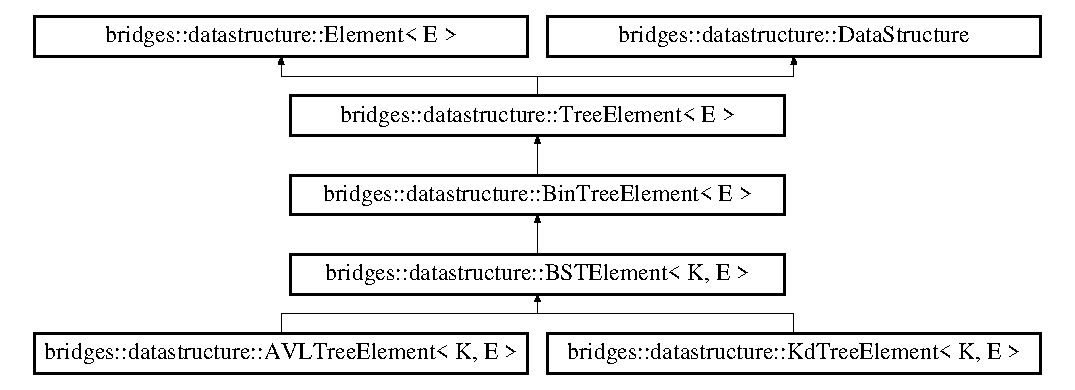
\includegraphics[height=4.794520cm]{classbridges_1_1datastructure_1_1_b_s_t_element}
\end{center}
\end{figure}


\subsection{Detailed Description}
\subsubsection*{template$<$typename K, typename E$>$\newline
class bridges\+::datastructure\+::\+B\+S\+T\+Element$<$ K, E $>$}

This class can be used to create binary search tree elements, derived from \hyperlink{classbridges_1_1datastructure_1_1_bin_tree_element}{Bin\+Tree\+Element}. 

This class extends the \hyperlink{classbridges_1_1datastructure_1_1_bin_tree_element}{Bin\+Tree\+Element} class by adding a \char`\"{}key\char`\"{} property to allow for use in a binary search tree implementation.

Generic Parameters\+: K that is the search key type, E the application data type

\begin{DoxySeeAlso}{See also}
There is a tutorial about Binary Search Trees \+: \href{http://bridgesuncc.github.io/tutorials/BinarySearchTree.html}{\tt http\+://bridgesuncc.\+github.\+io/tutorials/\+Binary\+Search\+Tree.\+html}
\end{DoxySeeAlso}
\begin{DoxyAuthor}{Author}
Kalpathi Subramanian 
\end{DoxyAuthor}
\begin{DoxyDate}{Date}
6/18/15, 7/17/16, 7/12/19 
\end{DoxyDate}
\subsection*{Public Member Functions}
\begin{DoxyCompactItemize}
\item 
\hyperlink{classbridges_1_1datastructure_1_1_b_s_t_element_a861caf985c223a9a848082fd5a4974fd}{B\+S\+T\+Element} (const K \&k, \hyperlink{classbridges_1_1datastructure_1_1_b_s_t_element}{B\+S\+T\+Element} $\ast$l, \hyperlink{classbridges_1_1datastructure_1_1_b_s_t_element}{B\+S\+T\+Element} $\ast$r, const E \&val=E(), const string \&lab=string())
\item 
\hyperlink{classbridges_1_1datastructure_1_1_b_s_t_element_a839372e61dd261d3fd7df1d22dd0a5dd}{B\+S\+T\+Element} (const K \&k, const E \&val=E(), const string \&lab=string())
\item 
virtual const string \hyperlink{classbridges_1_1datastructure_1_1_b_s_t_element_a2bb8cc9ec4b6bc5b89ecef0f17be366f}{get\+D\+Stype} () const override
\item 
K \hyperlink{classbridges_1_1datastructure_1_1_b_s_t_element_a66bd1d5874e4e0c8048e03e5fff07f86}{get\+Key} () const
\item 
void \hyperlink{classbridges_1_1datastructure_1_1_b_s_t_element_a06d80480736ae19052e2d1bc6345323a}{set\+Key} (const K \&k)
\item 
virtual \hyperlink{classbridges_1_1datastructure_1_1_b_s_t_element}{B\+S\+T\+Element} $\ast$ \hyperlink{classbridges_1_1datastructure_1_1_b_s_t_element_af863c624691c11db26ae3b6d723d1f5c}{get\+Left} () override
\item 
virtual const \hyperlink{classbridges_1_1datastructure_1_1_b_s_t_element}{B\+S\+T\+Element} $\ast$ \hyperlink{classbridges_1_1datastructure_1_1_b_s_t_element_abac324ef0b480420bd82ecfe4501d60d}{get\+Left} () const override
\item 
void \hyperlink{classbridges_1_1datastructure_1_1_b_s_t_element_a5810ed79b697d691f4d8a75c2f9b639f}{set\+Left} (\hyperlink{classbridges_1_1datastructure_1_1_b_s_t_element}{B\+S\+T\+Element} $\ast$l)
\item 
virtual \hyperlink{classbridges_1_1datastructure_1_1_b_s_t_element}{B\+S\+T\+Element} $\ast$ \hyperlink{classbridges_1_1datastructure_1_1_b_s_t_element_a80f5085d6d03805dd3091b7693d8e235}{get\+Right} () override
\item 
virtual const \hyperlink{classbridges_1_1datastructure_1_1_b_s_t_element}{B\+S\+T\+Element} $\ast$ \hyperlink{classbridges_1_1datastructure_1_1_b_s_t_element_a012f0eb09c3d62b14c73109e6ded0879}{get\+Right} () const override
\item 
void \hyperlink{classbridges_1_1datastructure_1_1_b_s_t_element_a9656227e934249edd0e414189c2cdae9}{set\+Right} (\hyperlink{classbridges_1_1datastructure_1_1_b_s_t_element}{B\+S\+T\+Element} $\ast$r)
\end{DoxyCompactItemize}
\subsection*{Protected Member Functions}
\begin{DoxyCompactItemize}
\item 
virtual const string \hyperlink{classbridges_1_1datastructure_1_1_b_s_t_element_a8f962a01b6e0eff59abeee7768264fd9}{get\+Element\+Representation} () const override
\end{DoxyCompactItemize}
\subsection*{Protected Attributes}
\begin{DoxyCompactItemize}
\item 
K \hyperlink{classbridges_1_1datastructure_1_1_b_s_t_element_ac1d971f8379c4ce6b956ebd635c88895}{key} = K()
\end{DoxyCompactItemize}
\subsection*{Additional Inherited Members}


\subsection{Constructor \& Destructor Documentation}
\mbox{\Hypertarget{classbridges_1_1datastructure_1_1_b_s_t_element_a861caf985c223a9a848082fd5a4974fd}\label{classbridges_1_1datastructure_1_1_b_s_t_element_a861caf985c223a9a848082fd5a4974fd}} 
\index{bridges\+::datastructure\+::\+B\+S\+T\+Element@{bridges\+::datastructure\+::\+B\+S\+T\+Element}!B\+S\+T\+Element@{B\+S\+T\+Element}}
\index{B\+S\+T\+Element@{B\+S\+T\+Element}!bridges\+::datastructure\+::\+B\+S\+T\+Element@{bridges\+::datastructure\+::\+B\+S\+T\+Element}}
\subsubsection{\texorpdfstring{B\+S\+T\+Element()}{BSTElement()}\hspace{0.1cm}{\footnotesize\ttfamily [1/2]}}
{\footnotesize\ttfamily template$<$typename K , typename E $>$ \\
\hyperlink{classbridges_1_1datastructure_1_1_b_s_t_element}{bridges\+::datastructure\+::\+B\+S\+T\+Element}$<$ K, E $>$\+::\hyperlink{classbridges_1_1datastructure_1_1_b_s_t_element}{B\+S\+T\+Element} (\begin{DoxyParamCaption}\item[{const K \&}]{k,  }\item[{\hyperlink{classbridges_1_1datastructure_1_1_b_s_t_element}{B\+S\+T\+Element}$<$ K, E $>$ $\ast$}]{l,  }\item[{\hyperlink{classbridges_1_1datastructure_1_1_b_s_t_element}{B\+S\+T\+Element}$<$ K, E $>$ $\ast$}]{r,  }\item[{const E \&}]{val = {\ttfamily E()},  }\item[{const string \&}]{lab = {\ttfamily string()} }\end{DoxyParamCaption})\hspace{0.3cm}{\ttfamily [inline]}}

Constructs a \hyperlink{classbridges_1_1datastructure_1_1_b_s_t_element}{B\+S\+T\+Element} with the provided value, label, key, left and right B\+S\+T\+Elements. The defaults will be used if not provided.


\begin{DoxyParams}{Parameters}
{\em k} & The key for ordering \\
\hline
{\em l} & The left \hyperlink{classbridges_1_1datastructure_1_1_b_s_t_element}{B\+S\+T\+Element} \\
\hline
{\em r} & The right \hyperlink{classbridges_1_1datastructure_1_1_b_s_t_element}{B\+S\+T\+Element} \\
\hline
{\em val} & The data to hold \\
\hline
{\em lab} & The label to show \\
\hline
\end{DoxyParams}
\mbox{\Hypertarget{classbridges_1_1datastructure_1_1_b_s_t_element_a839372e61dd261d3fd7df1d22dd0a5dd}\label{classbridges_1_1datastructure_1_1_b_s_t_element_a839372e61dd261d3fd7df1d22dd0a5dd}} 
\index{bridges\+::datastructure\+::\+B\+S\+T\+Element@{bridges\+::datastructure\+::\+B\+S\+T\+Element}!B\+S\+T\+Element@{B\+S\+T\+Element}}
\index{B\+S\+T\+Element@{B\+S\+T\+Element}!bridges\+::datastructure\+::\+B\+S\+T\+Element@{bridges\+::datastructure\+::\+B\+S\+T\+Element}}
\subsubsection{\texorpdfstring{B\+S\+T\+Element()}{BSTElement()}\hspace{0.1cm}{\footnotesize\ttfamily [2/2]}}
{\footnotesize\ttfamily template$<$typename K , typename E $>$ \\
\hyperlink{classbridges_1_1datastructure_1_1_b_s_t_element}{bridges\+::datastructure\+::\+B\+S\+T\+Element}$<$ K, E $>$\+::\hyperlink{classbridges_1_1datastructure_1_1_b_s_t_element}{B\+S\+T\+Element} (\begin{DoxyParamCaption}\item[{const K \&}]{k,  }\item[{const E \&}]{val = {\ttfamily E()},  }\item[{const string \&}]{lab = {\ttfamily string()} }\end{DoxyParamCaption})\hspace{0.3cm}{\ttfamily [inline]}}

Constructs a \hyperlink{classbridges_1_1datastructure_1_1_b_s_t_element}{B\+S\+T\+Element} with the provided value, label, key, setting the left and right B\+S\+T\+Elements to N\+U\+LL. The defaults will be used if not provided.


\begin{DoxyParams}{Parameters}
{\em k} & The key for ordering \\
\hline
{\em val} & The data to hold \\
\hline
{\em lab} & The label to show \\
\hline
\end{DoxyParams}


\subsection{Member Function Documentation}
\mbox{\Hypertarget{classbridges_1_1datastructure_1_1_b_s_t_element_a2bb8cc9ec4b6bc5b89ecef0f17be366f}\label{classbridges_1_1datastructure_1_1_b_s_t_element_a2bb8cc9ec4b6bc5b89ecef0f17be366f}} 
\index{bridges\+::datastructure\+::\+B\+S\+T\+Element@{bridges\+::datastructure\+::\+B\+S\+T\+Element}!get\+D\+Stype@{get\+D\+Stype}}
\index{get\+D\+Stype@{get\+D\+Stype}!bridges\+::datastructure\+::\+B\+S\+T\+Element@{bridges\+::datastructure\+::\+B\+S\+T\+Element}}
\subsubsection{\texorpdfstring{get\+D\+Stype()}{getDStype()}}
{\footnotesize\ttfamily template$<$typename K , typename E $>$ \\
virtual const string \hyperlink{classbridges_1_1datastructure_1_1_b_s_t_element}{bridges\+::datastructure\+::\+B\+S\+T\+Element}$<$ K, E $>$\+::get\+D\+Stype (\begin{DoxyParamCaption}{ }\end{DoxyParamCaption}) const\hspace{0.3cm}{\ttfamily [inline]}, {\ttfamily [override]}, {\ttfamily [virtual]}}

Returns the data structure name \begin{DoxyReturn}{Returns}
the data structure name 
\end{DoxyReturn}


Reimplemented from \hyperlink{classbridges_1_1datastructure_1_1_bin_tree_element_aef86e3663785972251547e409fdc757b}{bridges\+::datastructure\+::\+Bin\+Tree\+Element$<$ E $>$}.



Reimplemented in \hyperlink{classbridges_1_1datastructure_1_1_kd_tree_element_a76f6d9bfadfdec09d0a8564aa0e33235}{bridges\+::datastructure\+::\+Kd\+Tree\+Element$<$ K, E $>$}, and \hyperlink{classbridges_1_1datastructure_1_1_a_v_l_tree_element_ab04d1e9ad4630e408041e8137dc9854a}{bridges\+::datastructure\+::\+A\+V\+L\+Tree\+Element$<$ K, E $>$}.

\mbox{\Hypertarget{classbridges_1_1datastructure_1_1_b_s_t_element_a8f962a01b6e0eff59abeee7768264fd9}\label{classbridges_1_1datastructure_1_1_b_s_t_element_a8f962a01b6e0eff59abeee7768264fd9}} 
\index{bridges\+::datastructure\+::\+B\+S\+T\+Element@{bridges\+::datastructure\+::\+B\+S\+T\+Element}!get\+Element\+Representation@{get\+Element\+Representation}}
\index{get\+Element\+Representation@{get\+Element\+Representation}!bridges\+::datastructure\+::\+B\+S\+T\+Element@{bridges\+::datastructure\+::\+B\+S\+T\+Element}}
\subsubsection{\texorpdfstring{get\+Element\+Representation()}{getElementRepresentation()}}
{\footnotesize\ttfamily template$<$typename K , typename E $>$ \\
virtual const string \hyperlink{classbridges_1_1datastructure_1_1_b_s_t_element}{bridges\+::datastructure\+::\+B\+S\+T\+Element}$<$ K, E $>$\+::get\+Element\+Representation (\begin{DoxyParamCaption}{ }\end{DoxyParamCaption}) const\hspace{0.3cm}{\ttfamily [inline]}, {\ttfamily [override]}, {\ttfamily [protected]}, {\ttfamily [virtual]}}

Gets the J\+S\+ON representation of this element 

Reimplemented from \hyperlink{classbridges_1_1datastructure_1_1_element_a285fc51d6dfcb8bff2d72f7e4addfe6d}{bridges\+::datastructure\+::\+Element$<$ E $>$}.



Reimplemented in \hyperlink{classbridges_1_1datastructure_1_1_kd_tree_element_a5413ecaf152e3df5fb45dd85da812888}{bridges\+::datastructure\+::\+Kd\+Tree\+Element$<$ K, E $>$}.

\mbox{\Hypertarget{classbridges_1_1datastructure_1_1_b_s_t_element_a66bd1d5874e4e0c8048e03e5fff07f86}\label{classbridges_1_1datastructure_1_1_b_s_t_element_a66bd1d5874e4e0c8048e03e5fff07f86}} 
\index{bridges\+::datastructure\+::\+B\+S\+T\+Element@{bridges\+::datastructure\+::\+B\+S\+T\+Element}!get\+Key@{get\+Key}}
\index{get\+Key@{get\+Key}!bridges\+::datastructure\+::\+B\+S\+T\+Element@{bridges\+::datastructure\+::\+B\+S\+T\+Element}}
\subsubsection{\texorpdfstring{get\+Key()}{getKey()}}
{\footnotesize\ttfamily template$<$typename K , typename E $>$ \\
K \hyperlink{classbridges_1_1datastructure_1_1_b_s_t_element}{bridges\+::datastructure\+::\+B\+S\+T\+Element}$<$ K, E $>$\+::get\+Key (\begin{DoxyParamCaption}{ }\end{DoxyParamCaption}) const\hspace{0.3cm}{\ttfamily [inline]}}

Returns the key value \begin{DoxyReturn}{Returns}
The key of this \hyperlink{classbridges_1_1datastructure_1_1_b_s_t_element}{B\+S\+T\+Element} 
\end{DoxyReturn}
\mbox{\Hypertarget{classbridges_1_1datastructure_1_1_b_s_t_element_af863c624691c11db26ae3b6d723d1f5c}\label{classbridges_1_1datastructure_1_1_b_s_t_element_af863c624691c11db26ae3b6d723d1f5c}} 
\index{bridges\+::datastructure\+::\+B\+S\+T\+Element@{bridges\+::datastructure\+::\+B\+S\+T\+Element}!get\+Left@{get\+Left}}
\index{get\+Left@{get\+Left}!bridges\+::datastructure\+::\+B\+S\+T\+Element@{bridges\+::datastructure\+::\+B\+S\+T\+Element}}
\subsubsection{\texorpdfstring{get\+Left()}{getLeft()}\hspace{0.1cm}{\footnotesize\ttfamily [1/2]}}
{\footnotesize\ttfamily template$<$typename K , typename E $>$ \\
virtual \hyperlink{classbridges_1_1datastructure_1_1_b_s_t_element}{B\+S\+T\+Element}$\ast$ \hyperlink{classbridges_1_1datastructure_1_1_b_s_t_element}{bridges\+::datastructure\+::\+B\+S\+T\+Element}$<$ K, E $>$\+::get\+Left (\begin{DoxyParamCaption}{ }\end{DoxyParamCaption})\hspace{0.3cm}{\ttfamily [inline]}, {\ttfamily [override]}, {\ttfamily [virtual]}}

Return the left child \begin{DoxyReturn}{Returns}
The left child 
\end{DoxyReturn}


Reimplemented from \hyperlink{classbridges_1_1datastructure_1_1_bin_tree_element_ab30cfe373892c52709d5f1df013a0c82}{bridges\+::datastructure\+::\+Bin\+Tree\+Element$<$ E $>$}.



Reimplemented in \hyperlink{classbridges_1_1datastructure_1_1_kd_tree_element_a875bfa2dfd88a7740f7bcd28a117c12a}{bridges\+::datastructure\+::\+Kd\+Tree\+Element$<$ K, E $>$}, and \hyperlink{classbridges_1_1datastructure_1_1_a_v_l_tree_element_ab05925e343b9fa71b61c71e8034e1293}{bridges\+::datastructure\+::\+A\+V\+L\+Tree\+Element$<$ K, E $>$}.

\mbox{\Hypertarget{classbridges_1_1datastructure_1_1_b_s_t_element_abac324ef0b480420bd82ecfe4501d60d}\label{classbridges_1_1datastructure_1_1_b_s_t_element_abac324ef0b480420bd82ecfe4501d60d}} 
\index{bridges\+::datastructure\+::\+B\+S\+T\+Element@{bridges\+::datastructure\+::\+B\+S\+T\+Element}!get\+Left@{get\+Left}}
\index{get\+Left@{get\+Left}!bridges\+::datastructure\+::\+B\+S\+T\+Element@{bridges\+::datastructure\+::\+B\+S\+T\+Element}}
\subsubsection{\texorpdfstring{get\+Left()}{getLeft()}\hspace{0.1cm}{\footnotesize\ttfamily [2/2]}}
{\footnotesize\ttfamily template$<$typename K , typename E $>$ \\
virtual const \hyperlink{classbridges_1_1datastructure_1_1_b_s_t_element}{B\+S\+T\+Element}$\ast$ \hyperlink{classbridges_1_1datastructure_1_1_b_s_t_element}{bridges\+::datastructure\+::\+B\+S\+T\+Element}$<$ K, E $>$\+::get\+Left (\begin{DoxyParamCaption}{ }\end{DoxyParamCaption}) const\hspace{0.3cm}{\ttfamily [inline]}, {\ttfamily [override]}, {\ttfamily [virtual]}}

Return the left child -\/ Constant version

\begin{DoxyReturn}{Returns}
The left child 
\end{DoxyReturn}


Reimplemented from \hyperlink{classbridges_1_1datastructure_1_1_bin_tree_element_ae14a70e2d25ad62337c87059b0cadb48}{bridges\+::datastructure\+::\+Bin\+Tree\+Element$<$ E $>$}.



Reimplemented in \hyperlink{classbridges_1_1datastructure_1_1_kd_tree_element_a653597918fbc6e31b84fcf8dbdf67122}{bridges\+::datastructure\+::\+Kd\+Tree\+Element$<$ K, E $>$}, and \hyperlink{classbridges_1_1datastructure_1_1_a_v_l_tree_element_a4a639e0c623435aadf5c51ed132cb25d}{bridges\+::datastructure\+::\+A\+V\+L\+Tree\+Element$<$ K, E $>$}.

\mbox{\Hypertarget{classbridges_1_1datastructure_1_1_b_s_t_element_a80f5085d6d03805dd3091b7693d8e235}\label{classbridges_1_1datastructure_1_1_b_s_t_element_a80f5085d6d03805dd3091b7693d8e235}} 
\index{bridges\+::datastructure\+::\+B\+S\+T\+Element@{bridges\+::datastructure\+::\+B\+S\+T\+Element}!get\+Right@{get\+Right}}
\index{get\+Right@{get\+Right}!bridges\+::datastructure\+::\+B\+S\+T\+Element@{bridges\+::datastructure\+::\+B\+S\+T\+Element}}
\subsubsection{\texorpdfstring{get\+Right()}{getRight()}\hspace{0.1cm}{\footnotesize\ttfamily [1/2]}}
{\footnotesize\ttfamily template$<$typename K , typename E $>$ \\
virtual \hyperlink{classbridges_1_1datastructure_1_1_b_s_t_element}{B\+S\+T\+Element}$\ast$ \hyperlink{classbridges_1_1datastructure_1_1_b_s_t_element}{bridges\+::datastructure\+::\+B\+S\+T\+Element}$<$ K, E $>$\+::get\+Right (\begin{DoxyParamCaption}{ }\end{DoxyParamCaption})\hspace{0.3cm}{\ttfamily [inline]}, {\ttfamily [override]}, {\ttfamily [virtual]}}

Return the right child \begin{DoxyReturn}{Returns}
The right child 
\end{DoxyReturn}


Reimplemented from \hyperlink{classbridges_1_1datastructure_1_1_bin_tree_element_ae1e6bde8cc03cf5da5a7930354fdf592}{bridges\+::datastructure\+::\+Bin\+Tree\+Element$<$ E $>$}.



Reimplemented in \hyperlink{classbridges_1_1datastructure_1_1_kd_tree_element_a366e3b0987169220d3a145043be2373d}{bridges\+::datastructure\+::\+Kd\+Tree\+Element$<$ K, E $>$}, and \hyperlink{classbridges_1_1datastructure_1_1_a_v_l_tree_element_aed585fdf56fcbfebac6cd0262c9c1807}{bridges\+::datastructure\+::\+A\+V\+L\+Tree\+Element$<$ K, E $>$}.

\mbox{\Hypertarget{classbridges_1_1datastructure_1_1_b_s_t_element_a012f0eb09c3d62b14c73109e6ded0879}\label{classbridges_1_1datastructure_1_1_b_s_t_element_a012f0eb09c3d62b14c73109e6ded0879}} 
\index{bridges\+::datastructure\+::\+B\+S\+T\+Element@{bridges\+::datastructure\+::\+B\+S\+T\+Element}!get\+Right@{get\+Right}}
\index{get\+Right@{get\+Right}!bridges\+::datastructure\+::\+B\+S\+T\+Element@{bridges\+::datastructure\+::\+B\+S\+T\+Element}}
\subsubsection{\texorpdfstring{get\+Right()}{getRight()}\hspace{0.1cm}{\footnotesize\ttfamily [2/2]}}
{\footnotesize\ttfamily template$<$typename K , typename E $>$ \\
virtual const \hyperlink{classbridges_1_1datastructure_1_1_b_s_t_element}{B\+S\+T\+Element}$\ast$ \hyperlink{classbridges_1_1datastructure_1_1_b_s_t_element}{bridges\+::datastructure\+::\+B\+S\+T\+Element}$<$ K, E $>$\+::get\+Right (\begin{DoxyParamCaption}{ }\end{DoxyParamCaption}) const\hspace{0.3cm}{\ttfamily [inline]}, {\ttfamily [override]}, {\ttfamily [virtual]}}

Return the right child -\/ Constant version \begin{DoxyReturn}{Returns}
The right child 
\end{DoxyReturn}


Reimplemented from \hyperlink{classbridges_1_1datastructure_1_1_bin_tree_element_a795b1696d628b55dafb2bc1aa961843a}{bridges\+::datastructure\+::\+Bin\+Tree\+Element$<$ E $>$}.



Reimplemented in \hyperlink{classbridges_1_1datastructure_1_1_kd_tree_element_ae8d6007d3848b72cbfc11d2e29120781}{bridges\+::datastructure\+::\+Kd\+Tree\+Element$<$ K, E $>$}, and \hyperlink{classbridges_1_1datastructure_1_1_a_v_l_tree_element_a5a2c4b96b51da1daa3c0426882250acb}{bridges\+::datastructure\+::\+A\+V\+L\+Tree\+Element$<$ K, E $>$}.

\mbox{\Hypertarget{classbridges_1_1datastructure_1_1_b_s_t_element_a06d80480736ae19052e2d1bc6345323a}\label{classbridges_1_1datastructure_1_1_b_s_t_element_a06d80480736ae19052e2d1bc6345323a}} 
\index{bridges\+::datastructure\+::\+B\+S\+T\+Element@{bridges\+::datastructure\+::\+B\+S\+T\+Element}!set\+Key@{set\+Key}}
\index{set\+Key@{set\+Key}!bridges\+::datastructure\+::\+B\+S\+T\+Element@{bridges\+::datastructure\+::\+B\+S\+T\+Element}}
\subsubsection{\texorpdfstring{set\+Key()}{setKey()}}
{\footnotesize\ttfamily template$<$typename K , typename E $>$ \\
void \hyperlink{classbridges_1_1datastructure_1_1_b_s_t_element}{bridges\+::datastructure\+::\+B\+S\+T\+Element}$<$ K, E $>$\+::set\+Key (\begin{DoxyParamCaption}\item[{const K \&}]{k }\end{DoxyParamCaption})\hspace{0.3cm}{\ttfamily [inline]}}

Set key to \char`\"{}k\char`\"{}


\begin{DoxyParams}{Parameters}
{\em k} & The key of this \hyperlink{classbridges_1_1datastructure_1_1_b_s_t_element}{B\+S\+T\+Element} \\
\hline
\end{DoxyParams}
\mbox{\Hypertarget{classbridges_1_1datastructure_1_1_b_s_t_element_a5810ed79b697d691f4d8a75c2f9b639f}\label{classbridges_1_1datastructure_1_1_b_s_t_element_a5810ed79b697d691f4d8a75c2f9b639f}} 
\index{bridges\+::datastructure\+::\+B\+S\+T\+Element@{bridges\+::datastructure\+::\+B\+S\+T\+Element}!set\+Left@{set\+Left}}
\index{set\+Left@{set\+Left}!bridges\+::datastructure\+::\+B\+S\+T\+Element@{bridges\+::datastructure\+::\+B\+S\+T\+Element}}
\subsubsection{\texorpdfstring{set\+Left()}{setLeft()}}
{\footnotesize\ttfamily template$<$typename K , typename E $>$ \\
void \hyperlink{classbridges_1_1datastructure_1_1_b_s_t_element}{bridges\+::datastructure\+::\+B\+S\+T\+Element}$<$ K, E $>$\+::set\+Left (\begin{DoxyParamCaption}\item[{\hyperlink{classbridges_1_1datastructure_1_1_b_s_t_element}{B\+S\+T\+Element}$<$ K, E $>$ $\ast$}]{l }\end{DoxyParamCaption})\hspace{0.3cm}{\ttfamily [inline]}}

Sets left to \char`\"{}l\char`\"{}


\begin{DoxyParams}{Parameters}
{\em l} & The left child \\
\hline
\end{DoxyParams}
\mbox{\Hypertarget{classbridges_1_1datastructure_1_1_b_s_t_element_a9656227e934249edd0e414189c2cdae9}\label{classbridges_1_1datastructure_1_1_b_s_t_element_a9656227e934249edd0e414189c2cdae9}} 
\index{bridges\+::datastructure\+::\+B\+S\+T\+Element@{bridges\+::datastructure\+::\+B\+S\+T\+Element}!set\+Right@{set\+Right}}
\index{set\+Right@{set\+Right}!bridges\+::datastructure\+::\+B\+S\+T\+Element@{bridges\+::datastructure\+::\+B\+S\+T\+Element}}
\subsubsection{\texorpdfstring{set\+Right()}{setRight()}}
{\footnotesize\ttfamily template$<$typename K , typename E $>$ \\
void \hyperlink{classbridges_1_1datastructure_1_1_b_s_t_element}{bridges\+::datastructure\+::\+B\+S\+T\+Element}$<$ K, E $>$\+::set\+Right (\begin{DoxyParamCaption}\item[{\hyperlink{classbridges_1_1datastructure_1_1_b_s_t_element}{B\+S\+T\+Element}$<$ K, E $>$ $\ast$}]{r }\end{DoxyParamCaption})\hspace{0.3cm}{\ttfamily [inline]}}

Sets right child to \char`\"{}r\char`\"{}


\begin{DoxyParams}{Parameters}
{\em r} & The right \hyperlink{classbridges_1_1datastructure_1_1_b_s_t_element}{B\+S\+T\+Element} \\
\hline
\end{DoxyParams}


\subsection{Member Data Documentation}
\mbox{\Hypertarget{classbridges_1_1datastructure_1_1_b_s_t_element_ac1d971f8379c4ce6b956ebd635c88895}\label{classbridges_1_1datastructure_1_1_b_s_t_element_ac1d971f8379c4ce6b956ebd635c88895}} 
\index{bridges\+::datastructure\+::\+B\+S\+T\+Element@{bridges\+::datastructure\+::\+B\+S\+T\+Element}!key@{key}}
\index{key@{key}!bridges\+::datastructure\+::\+B\+S\+T\+Element@{bridges\+::datastructure\+::\+B\+S\+T\+Element}}
\subsubsection{\texorpdfstring{key}{key}}
{\footnotesize\ttfamily template$<$typename K , typename E $>$ \\
K \hyperlink{classbridges_1_1datastructure_1_1_b_s_t_element}{bridges\+::datastructure\+::\+B\+S\+T\+Element}$<$ K, E $>$\+::key = K()\hspace{0.3cm}{\ttfamily [protected]}}



The documentation for this class was generated from the following file\+:\begin{DoxyCompactItemize}
\item 
/home/erik/work/bridges/bridges-\/cxx/src/\hyperlink{_b_s_t_element_8h}{B\+S\+T\+Element.\+h}\end{DoxyCompactItemize}

\hypertarget{classbridges_1_1datastructure_1_1_b_t_element}{}\section{bridges\+:\+:datastructure\+:\+:B\+T\+Element$<$ E $>$ Class Template Reference}
\label{classbridges_1_1datastructure_1_1_b_t_element}\index{bridges\+::datastructure\+::\+B\+T\+Element$<$ E $>$@{bridges\+::datastructure\+::\+B\+T\+Element$<$ E $>$}}


{\ttfamily \#include $<$B\+T\+Element.\+h$>$}

Inheritance diagram for bridges\+:\+:datastructure\+:\+:B\+T\+Element$<$ E $>$\+:\begin{figure}[H]
\begin{center}
\leavevmode
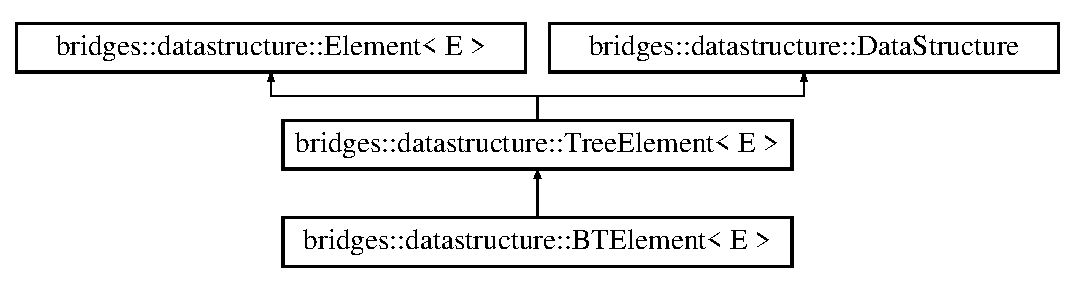
\includegraphics[height=3.000000cm]{classbridges_1_1datastructure_1_1_b_t_element}
\end{center}
\end{figure}


\subsection{Detailed Description}
\subsubsection*{template$<$typename E$>$\newline
class bridges\+::datastructure\+::\+B\+T\+Element$<$ E $>$}

This class can be used to create binary tree elements, derived from \mbox{\hyperlink{classbridges_1_1datastructure_1_1_tree_element}{Tree\+Element}}. 

This class can be used to create binary tree elements, with left and right subtrees


\begin{DoxyParams}{Parameters}
{\em E} & the application data type\\
\hline
\end{DoxyParams}
\begin{DoxyAuthor}{Author}
Kalpathi Subramanian 
\end{DoxyAuthor}
\begin{DoxyDate}{Date}
6/12/15 
\end{DoxyDate}
\subsection*{Public Member Functions}
\begin{DoxyCompactItemize}
\item 
\mbox{\hyperlink{classbridges_1_1datastructure_1_1_b_t_element_a7d93a35b1f2553cfd92a289a363caa5a}{B\+T\+Element}} (\mbox{\hyperlink{classbridges_1_1datastructure_1_1_b_t_element}{B\+T\+Element}} $\ast$l, \mbox{\hyperlink{classbridges_1_1datastructure_1_1_b_t_element}{B\+T\+Element}} $\ast$r, const E \&e=E(), const string \&lab=string())
\begin{DoxyCompactList}\small\item\em Constructs a \mbox{\hyperlink{classbridges_1_1datastructure_1_1_b_t_element}{B\+T\+Element}} with the provided value, label, left and right B\+T\+Elements. \end{DoxyCompactList}\item 
\mbox{\hyperlink{classbridges_1_1datastructure_1_1_b_t_element_a1bea31e483a1bf737e5da5cc9178bc3d}{B\+T\+Element}} (const E \&e=E(), const string \&lab=string())
\begin{DoxyCompactList}\small\item\em Constructs a \mbox{\hyperlink{classbridges_1_1datastructure_1_1_b_t_element}{B\+T\+Element}} with the provided value and label, setting the left and right \mbox{\hyperlink{classbridges_1_1datastructure_1_1_b_t_element}{B\+T\+Element}} to nullptr. \end{DoxyCompactList}\item 
virtual const string \mbox{\hyperlink{classbridges_1_1datastructure_1_1_b_t_element_a2118b6b74f3fe0fec39e3b258a7dee89}{get\+D\+Stype}} () const override
\item 
virtual \mbox{\hyperlink{classbridges_1_1datastructure_1_1_b_t_element}{B\+T\+Element}} $\ast$ \mbox{\hyperlink{classbridges_1_1datastructure_1_1_b_t_element_aaa551a4f24bb7ed63fd39e9c4153402b}{get\+Left}} ()
\item 
virtual const \mbox{\hyperlink{classbridges_1_1datastructure_1_1_b_t_element}{B\+T\+Element}} $\ast$ \mbox{\hyperlink{classbridges_1_1datastructure_1_1_b_t_element_aa13df422de48c6297223c3c28caf9277}{get\+Left}} () const
\item 
void \mbox{\hyperlink{classbridges_1_1datastructure_1_1_b_t_element_a6baeb1237f1879eb6a04fc144a7b55d6}{set\+Left}} (\mbox{\hyperlink{classbridges_1_1datastructure_1_1_b_t_element}{B\+T\+Element}} $\ast$l)
\item 
virtual \mbox{\hyperlink{classbridges_1_1datastructure_1_1_b_t_element}{B\+T\+Element}} $\ast$ \mbox{\hyperlink{classbridges_1_1datastructure_1_1_b_t_element_a3f73fcc5a7ed1af1a628803879682f80}{get\+Right}} ()
\item 
virtual const \mbox{\hyperlink{classbridges_1_1datastructure_1_1_b_t_element}{B\+T\+Element}} $\ast$ \mbox{\hyperlink{classbridges_1_1datastructure_1_1_b_t_element_afc0f4e1454bbdfb6a61ae9acf606e22a}{get\+Right}} () const
\item 
void \mbox{\hyperlink{classbridges_1_1datastructure_1_1_b_t_element_a016dfb73d148418ba581cfec96375db3}{set\+Right}} (\mbox{\hyperlink{classbridges_1_1datastructure_1_1_b_t_element}{B\+T\+Element}} $\ast$r)
\end{DoxyCompactItemize}
\subsection*{Additional Inherited Members}


\subsection{Constructor \& Destructor Documentation}
\mbox{\Hypertarget{classbridges_1_1datastructure_1_1_b_t_element_a7d93a35b1f2553cfd92a289a363caa5a}\label{classbridges_1_1datastructure_1_1_b_t_element_a7d93a35b1f2553cfd92a289a363caa5a}} 
\index{bridges\+::datastructure\+::\+B\+T\+Element@{bridges\+::datastructure\+::\+B\+T\+Element}!B\+T\+Element@{B\+T\+Element}}
\index{B\+T\+Element@{B\+T\+Element}!bridges\+::datastructure\+::\+B\+T\+Element@{bridges\+::datastructure\+::\+B\+T\+Element}}
\subsubsection{\texorpdfstring{B\+T\+Element()}{BTElement()}\hspace{0.1cm}{\footnotesize\ttfamily [1/2]}}
{\footnotesize\ttfamily template$<$typename E $>$ \\
\mbox{\hyperlink{classbridges_1_1datastructure_1_1_b_t_element}{bridges\+::datastructure\+::\+B\+T\+Element}}$<$ E $>$\+::\mbox{\hyperlink{classbridges_1_1datastructure_1_1_b_t_element}{B\+T\+Element}} (\begin{DoxyParamCaption}\item[{\mbox{\hyperlink{classbridges_1_1datastructure_1_1_b_t_element}{B\+T\+Element}}$<$ E $>$ $\ast$}]{l,  }\item[{\mbox{\hyperlink{classbridges_1_1datastructure_1_1_b_t_element}{B\+T\+Element}}$<$ E $>$ $\ast$}]{r,  }\item[{const E \&}]{e = {\ttfamily E()},  }\item[{const string \&}]{lab = {\ttfamily string()} }\end{DoxyParamCaption})\hspace{0.3cm}{\ttfamily [inline]}}



Constructs a \mbox{\hyperlink{classbridges_1_1datastructure_1_1_b_t_element}{B\+T\+Element}} with the provided value, label, left and right B\+T\+Elements. 

The defaults will be used if not provided.


\begin{DoxyParams}{Parameters}
{\em l} & The left \mbox{\hyperlink{classbridges_1_1datastructure_1_1_tree_element}{Tree\+Element}} \\
\hline
{\em r} & The right \mbox{\hyperlink{classbridges_1_1datastructure_1_1_tree_element}{Tree\+Element}} \\
\hline
{\em e} & The data to hold \\
\hline
{\em lab} & The label to show \\
\hline
\end{DoxyParams}
\mbox{\Hypertarget{classbridges_1_1datastructure_1_1_b_t_element_a1bea31e483a1bf737e5da5cc9178bc3d}\label{classbridges_1_1datastructure_1_1_b_t_element_a1bea31e483a1bf737e5da5cc9178bc3d}} 
\index{bridges\+::datastructure\+::\+B\+T\+Element@{bridges\+::datastructure\+::\+B\+T\+Element}!B\+T\+Element@{B\+T\+Element}}
\index{B\+T\+Element@{B\+T\+Element}!bridges\+::datastructure\+::\+B\+T\+Element@{bridges\+::datastructure\+::\+B\+T\+Element}}
\subsubsection{\texorpdfstring{B\+T\+Element()}{BTElement()}\hspace{0.1cm}{\footnotesize\ttfamily [2/2]}}
{\footnotesize\ttfamily template$<$typename E $>$ \\
\mbox{\hyperlink{classbridges_1_1datastructure_1_1_b_t_element}{bridges\+::datastructure\+::\+B\+T\+Element}}$<$ E $>$\+::\mbox{\hyperlink{classbridges_1_1datastructure_1_1_b_t_element}{B\+T\+Element}} (\begin{DoxyParamCaption}\item[{const E \&}]{e = {\ttfamily E()},  }\item[{const string \&}]{lab = {\ttfamily string()} }\end{DoxyParamCaption})\hspace{0.3cm}{\ttfamily [inline]}}



Constructs a \mbox{\hyperlink{classbridges_1_1datastructure_1_1_b_t_element}{B\+T\+Element}} with the provided value and label, setting the left and right \mbox{\hyperlink{classbridges_1_1datastructure_1_1_b_t_element}{B\+T\+Element}} to nullptr. 

The defaults will be used if not provided.


\begin{DoxyParams}{Parameters}
{\em e} & The data to hold \\
\hline
{\em lab} & The label to show \\
\hline
\end{DoxyParams}


\subsection{Member Function Documentation}
\mbox{\Hypertarget{classbridges_1_1datastructure_1_1_b_t_element_a2118b6b74f3fe0fec39e3b258a7dee89}\label{classbridges_1_1datastructure_1_1_b_t_element_a2118b6b74f3fe0fec39e3b258a7dee89}} 
\index{bridges\+::datastructure\+::\+B\+T\+Element@{bridges\+::datastructure\+::\+B\+T\+Element}!get\+D\+Stype@{get\+D\+Stype}}
\index{get\+D\+Stype@{get\+D\+Stype}!bridges\+::datastructure\+::\+B\+T\+Element@{bridges\+::datastructure\+::\+B\+T\+Element}}
\subsubsection{\texorpdfstring{get\+D\+Stype()}{getDStype()}}
{\footnotesize\ttfamily template$<$typename E $>$ \\
virtual const string \mbox{\hyperlink{classbridges_1_1datastructure_1_1_b_t_element}{bridges\+::datastructure\+::\+B\+T\+Element}}$<$ E $>$\+::get\+D\+Stype (\begin{DoxyParamCaption}{ }\end{DoxyParamCaption}) const\hspace{0.3cm}{\ttfamily [inline]}, {\ttfamily [override]}, {\ttfamily [virtual]}}

\begin{DoxyReturn}{Returns}
the data structure type 
\end{DoxyReturn}


Reimplemented from \mbox{\hyperlink{classbridges_1_1datastructure_1_1_tree_element_a897f34ea284da45e1dc869c3e3b6c9a4}{bridges\+::datastructure\+::\+Tree\+Element$<$ E $>$}}.

\mbox{\Hypertarget{classbridges_1_1datastructure_1_1_b_t_element_aaa551a4f24bb7ed63fd39e9c4153402b}\label{classbridges_1_1datastructure_1_1_b_t_element_aaa551a4f24bb7ed63fd39e9c4153402b}} 
\index{bridges\+::datastructure\+::\+B\+T\+Element@{bridges\+::datastructure\+::\+B\+T\+Element}!get\+Left@{get\+Left}}
\index{get\+Left@{get\+Left}!bridges\+::datastructure\+::\+B\+T\+Element@{bridges\+::datastructure\+::\+B\+T\+Element}}
\subsubsection{\texorpdfstring{get\+Left()}{getLeft()}\hspace{0.1cm}{\footnotesize\ttfamily [1/2]}}
{\footnotesize\ttfamily template$<$typename E $>$ \\
virtual \mbox{\hyperlink{classbridges_1_1datastructure_1_1_b_t_element}{B\+T\+Element}}$\ast$ \mbox{\hyperlink{classbridges_1_1datastructure_1_1_b_t_element}{bridges\+::datastructure\+::\+B\+T\+Element}}$<$ E $>$\+::get\+Left (\begin{DoxyParamCaption}{ }\end{DoxyParamCaption})\hspace{0.3cm}{\ttfamily [inline]}, {\ttfamily [virtual]}}

\begin{DoxyReturn}{Returns}
The left \mbox{\hyperlink{classbridges_1_1datastructure_1_1_b_t_element}{B\+T\+Element}} 
\end{DoxyReturn}
\mbox{\Hypertarget{classbridges_1_1datastructure_1_1_b_t_element_aa13df422de48c6297223c3c28caf9277}\label{classbridges_1_1datastructure_1_1_b_t_element_aa13df422de48c6297223c3c28caf9277}} 
\index{bridges\+::datastructure\+::\+B\+T\+Element@{bridges\+::datastructure\+::\+B\+T\+Element}!get\+Left@{get\+Left}}
\index{get\+Left@{get\+Left}!bridges\+::datastructure\+::\+B\+T\+Element@{bridges\+::datastructure\+::\+B\+T\+Element}}
\subsubsection{\texorpdfstring{get\+Left()}{getLeft()}\hspace{0.1cm}{\footnotesize\ttfamily [2/2]}}
{\footnotesize\ttfamily template$<$typename E $>$ \\
virtual const \mbox{\hyperlink{classbridges_1_1datastructure_1_1_b_t_element}{B\+T\+Element}}$\ast$ \mbox{\hyperlink{classbridges_1_1datastructure_1_1_b_t_element}{bridges\+::datastructure\+::\+B\+T\+Element}}$<$ E $>$\+::get\+Left (\begin{DoxyParamCaption}{ }\end{DoxyParamCaption}) const\hspace{0.3cm}{\ttfamily [inline]}, {\ttfamily [virtual]}}

Constant version \mbox{\Hypertarget{classbridges_1_1datastructure_1_1_b_t_element_a3f73fcc5a7ed1af1a628803879682f80}\label{classbridges_1_1datastructure_1_1_b_t_element_a3f73fcc5a7ed1af1a628803879682f80}} 
\index{bridges\+::datastructure\+::\+B\+T\+Element@{bridges\+::datastructure\+::\+B\+T\+Element}!get\+Right@{get\+Right}}
\index{get\+Right@{get\+Right}!bridges\+::datastructure\+::\+B\+T\+Element@{bridges\+::datastructure\+::\+B\+T\+Element}}
\subsubsection{\texorpdfstring{get\+Right()}{getRight()}\hspace{0.1cm}{\footnotesize\ttfamily [1/2]}}
{\footnotesize\ttfamily template$<$typename E $>$ \\
virtual \mbox{\hyperlink{classbridges_1_1datastructure_1_1_b_t_element}{B\+T\+Element}}$\ast$ \mbox{\hyperlink{classbridges_1_1datastructure_1_1_b_t_element}{bridges\+::datastructure\+::\+B\+T\+Element}}$<$ E $>$\+::get\+Right (\begin{DoxyParamCaption}{ }\end{DoxyParamCaption})\hspace{0.3cm}{\ttfamily [inline]}, {\ttfamily [virtual]}}

\begin{DoxyReturn}{Returns}
The right \mbox{\hyperlink{classbridges_1_1datastructure_1_1_b_t_element}{B\+T\+Element}} 
\end{DoxyReturn}
\mbox{\Hypertarget{classbridges_1_1datastructure_1_1_b_t_element_afc0f4e1454bbdfb6a61ae9acf606e22a}\label{classbridges_1_1datastructure_1_1_b_t_element_afc0f4e1454bbdfb6a61ae9acf606e22a}} 
\index{bridges\+::datastructure\+::\+B\+T\+Element@{bridges\+::datastructure\+::\+B\+T\+Element}!get\+Right@{get\+Right}}
\index{get\+Right@{get\+Right}!bridges\+::datastructure\+::\+B\+T\+Element@{bridges\+::datastructure\+::\+B\+T\+Element}}
\subsubsection{\texorpdfstring{get\+Right()}{getRight()}\hspace{0.1cm}{\footnotesize\ttfamily [2/2]}}
{\footnotesize\ttfamily template$<$typename E $>$ \\
virtual const \mbox{\hyperlink{classbridges_1_1datastructure_1_1_b_t_element}{B\+T\+Element}}$\ast$ \mbox{\hyperlink{classbridges_1_1datastructure_1_1_b_t_element}{bridges\+::datastructure\+::\+B\+T\+Element}}$<$ E $>$\+::get\+Right (\begin{DoxyParamCaption}{ }\end{DoxyParamCaption}) const\hspace{0.3cm}{\ttfamily [inline]}, {\ttfamily [virtual]}}

Constant version \mbox{\Hypertarget{classbridges_1_1datastructure_1_1_b_t_element_a6baeb1237f1879eb6a04fc144a7b55d6}\label{classbridges_1_1datastructure_1_1_b_t_element_a6baeb1237f1879eb6a04fc144a7b55d6}} 
\index{bridges\+::datastructure\+::\+B\+T\+Element@{bridges\+::datastructure\+::\+B\+T\+Element}!set\+Left@{set\+Left}}
\index{set\+Left@{set\+Left}!bridges\+::datastructure\+::\+B\+T\+Element@{bridges\+::datastructure\+::\+B\+T\+Element}}
\subsubsection{\texorpdfstring{set\+Left()}{setLeft()}}
{\footnotesize\ttfamily template$<$typename E $>$ \\
void \mbox{\hyperlink{classbridges_1_1datastructure_1_1_b_t_element}{bridges\+::datastructure\+::\+B\+T\+Element}}$<$ E $>$\+::set\+Left (\begin{DoxyParamCaption}\item[{\mbox{\hyperlink{classbridges_1_1datastructure_1_1_b_t_element}{B\+T\+Element}}$<$ E $>$ $\ast$}]{l }\end{DoxyParamCaption})\hspace{0.3cm}{\ttfamily [inline]}}

Sets left to \char`\"{}l\char`\"{}
\begin{DoxyParams}{Parameters}
{\em l} & The left \mbox{\hyperlink{classbridges_1_1datastructure_1_1_b_t_element}{B\+T\+Element}} \\
\hline
\end{DoxyParams}
\mbox{\Hypertarget{classbridges_1_1datastructure_1_1_b_t_element_a016dfb73d148418ba581cfec96375db3}\label{classbridges_1_1datastructure_1_1_b_t_element_a016dfb73d148418ba581cfec96375db3}} 
\index{bridges\+::datastructure\+::\+B\+T\+Element@{bridges\+::datastructure\+::\+B\+T\+Element}!set\+Right@{set\+Right}}
\index{set\+Right@{set\+Right}!bridges\+::datastructure\+::\+B\+T\+Element@{bridges\+::datastructure\+::\+B\+T\+Element}}
\subsubsection{\texorpdfstring{set\+Right()}{setRight()}}
{\footnotesize\ttfamily template$<$typename E $>$ \\
void \mbox{\hyperlink{classbridges_1_1datastructure_1_1_b_t_element}{bridges\+::datastructure\+::\+B\+T\+Element}}$<$ E $>$\+::set\+Right (\begin{DoxyParamCaption}\item[{\mbox{\hyperlink{classbridges_1_1datastructure_1_1_b_t_element}{B\+T\+Element}}$<$ E $>$ $\ast$}]{r }\end{DoxyParamCaption})\hspace{0.3cm}{\ttfamily [inline]}}

Sets right to \char`\"{}r\char`\"{}
\begin{DoxyParams}{Parameters}
{\em r} & The right \mbox{\hyperlink{classbridges_1_1datastructure_1_1_b_t_element}{B\+T\+Element}} \\
\hline
\end{DoxyParams}


The documentation for this class was generated from the following file\+:\begin{DoxyCompactItemize}
\item 
/\+Users/kalpathi/gr/bridges/client/cxx/src/\mbox{\hyperlink{_b_t_element_8h}{B\+T\+Element.\+h}}\end{DoxyCompactItemize}

\hypertarget{classbridges_1_1_cache}{}\doxysection{bridges\+::Cache Class Reference}
\label{classbridges_1_1_cache}\index{bridges::Cache@{bridges::Cache}}


{\ttfamily \#include $<$Cache.\+h$>$}

Inheritance diagram for bridges\+::Cache\+:\begin{figure}[H]
\begin{center}
\leavevmode
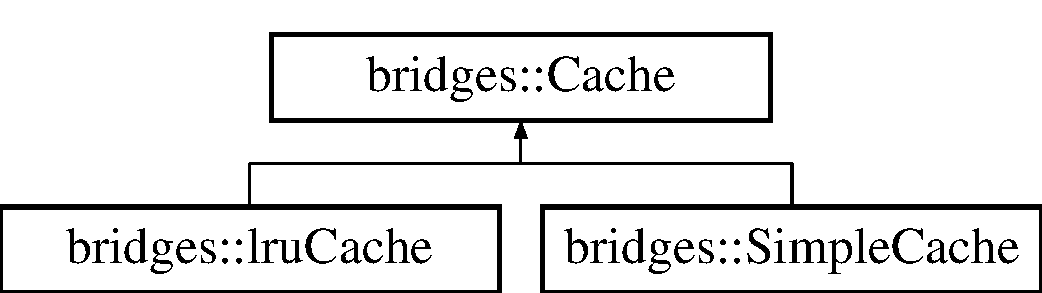
\includegraphics[height=2.000000cm]{classbridges_1_1_cache}
\end{center}
\end{figure}
\doxysubsection*{Public Member Functions}
\begin{DoxyCompactItemize}
\item 
virtual bool \mbox{\hyperlink{classbridges_1_1_cache_abf3601225841d14dcd5611cd6a223ba4}{in\+Cache}} (const std\+::string \&doc\+Name) noexcept(false)=0
\item 
virtual std\+::string \mbox{\hyperlink{classbridges_1_1_cache_abc1eaca36899e6e85df1c9a690f1d4dd}{get\+Doc}} (const std\+::string \&doc\+Name) noexcept(false)=0
\item 
virtual void \mbox{\hyperlink{classbridges_1_1_cache_ae74225542568a377fdcaf0354e466954}{put\+Doc}} (const std\+::string \&doc\+Name, const std\+::string \&content) noexcept(false)=0
\end{DoxyCompactItemize}


\doxysubsection{Member Function Documentation}
\mbox{\Hypertarget{classbridges_1_1_cache_abc1eaca36899e6e85df1c9a690f1d4dd}\label{classbridges_1_1_cache_abc1eaca36899e6e85df1c9a690f1d4dd}} 
\index{bridges::Cache@{bridges::Cache}!getDoc@{getDoc}}
\index{getDoc@{getDoc}!bridges::Cache@{bridges::Cache}}
\doxysubsubsection{\texorpdfstring{getDoc()}{getDoc()}}
{\footnotesize\ttfamily virtual std\+::string bridges\+::\+Cache\+::get\+Doc (\begin{DoxyParamCaption}\item[{const std\+::string \&}]{doc\+Name }\end{DoxyParamCaption})\hspace{0.3cm}{\ttfamily [pure virtual]}, {\ttfamily [noexcept]}}



Implemented in \mbox{\hyperlink{classbridges_1_1lru_cache_ac8bed8ab7cbf002a23573c071ba04ad6}{bridges\+::lru\+Cache}}, and \mbox{\hyperlink{classbridges_1_1_simple_cache_a905ad2e7fb1b6784a5f70caf024b157f}{bridges\+::\+Simple\+Cache}}.

\mbox{\Hypertarget{classbridges_1_1_cache_abf3601225841d14dcd5611cd6a223ba4}\label{classbridges_1_1_cache_abf3601225841d14dcd5611cd6a223ba4}} 
\index{bridges::Cache@{bridges::Cache}!inCache@{inCache}}
\index{inCache@{inCache}!bridges::Cache@{bridges::Cache}}
\doxysubsubsection{\texorpdfstring{inCache()}{inCache()}}
{\footnotesize\ttfamily virtual bool bridges\+::\+Cache\+::in\+Cache (\begin{DoxyParamCaption}\item[{const std\+::string \&}]{doc\+Name }\end{DoxyParamCaption})\hspace{0.3cm}{\ttfamily [pure virtual]}, {\ttfamily [noexcept]}}



Implemented in \mbox{\hyperlink{classbridges_1_1lru_cache_ab56c75166ddcc3d17e6924e581f7a4e8}{bridges\+::lru\+Cache}}, and \mbox{\hyperlink{classbridges_1_1_simple_cache_a9af328045bad7c3bd4ed6cf99352bf07}{bridges\+::\+Simple\+Cache}}.

\mbox{\Hypertarget{classbridges_1_1_cache_ae74225542568a377fdcaf0354e466954}\label{classbridges_1_1_cache_ae74225542568a377fdcaf0354e466954}} 
\index{bridges::Cache@{bridges::Cache}!putDoc@{putDoc}}
\index{putDoc@{putDoc}!bridges::Cache@{bridges::Cache}}
\doxysubsubsection{\texorpdfstring{putDoc()}{putDoc()}}
{\footnotesize\ttfamily virtual void bridges\+::\+Cache\+::put\+Doc (\begin{DoxyParamCaption}\item[{const std\+::string \&}]{doc\+Name,  }\item[{const std\+::string \&}]{content }\end{DoxyParamCaption})\hspace{0.3cm}{\ttfamily [pure virtual]}, {\ttfamily [noexcept]}}



Implemented in \mbox{\hyperlink{classbridges_1_1lru_cache_a927fa1186ba830717ce11898c2beb4c7}{bridges\+::lru\+Cache}}, and \mbox{\hyperlink{classbridges_1_1_simple_cache_a61264b1080a4458d6210c7cf6b4e8615}{bridges\+::\+Simple\+Cache}}.



The documentation for this class was generated from the following file\+:\begin{DoxyCompactItemize}
\item 
/home/erik/work/bridges/bridges-\/cxx/src/\mbox{\hyperlink{_cache_8h}{Cache.\+h}}\end{DoxyCompactItemize}

\hypertarget{classbridges_1_1_cache_exception}{}\section{bridges\+:\+:Cache\+Exception Class Reference}
\label{classbridges_1_1_cache_exception}\index{bridges\+::\+Cache\+Exception@{bridges\+::\+Cache\+Exception}}


{\ttfamily \#include $<$Data\+Source.\+h$>$}

Inheritance diagram for bridges\+:\+:Cache\+Exception\+:\begin{figure}[H]
\begin{center}
\leavevmode
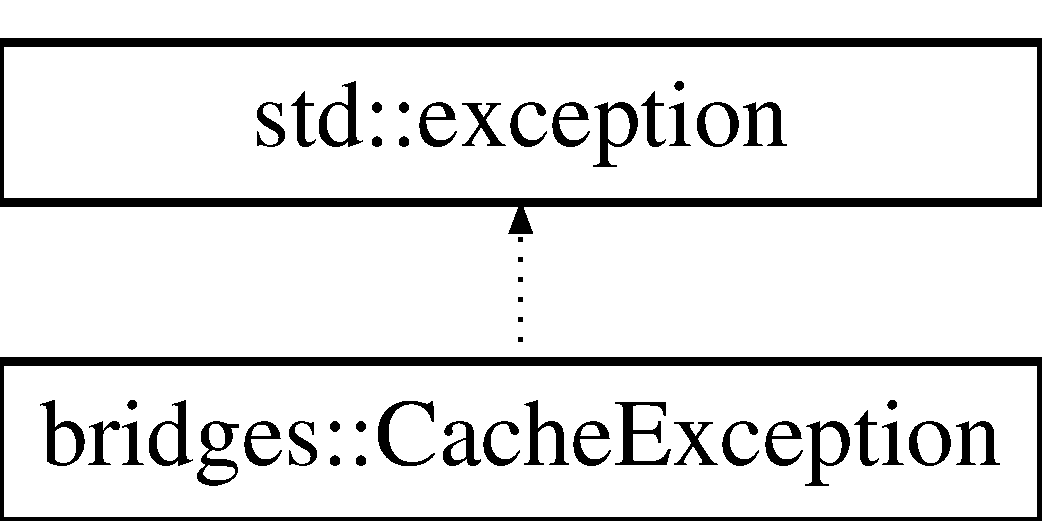
\includegraphics[height=2.000000cm]{classbridges_1_1_cache_exception}
\end{center}
\end{figure}


The documentation for this class was generated from the following file\+:\begin{DoxyCompactItemize}
\item 
/\+Users/kalpathi/gr/bridges/client/cxx/bridges18/src/\mbox{\hyperlink{_data_source_8h}{Data\+Source.\+h}}\end{DoxyCompactItemize}

\hypertarget{classbridges_1_1dataset_1_1_cancer_incidence}{}\section{bridges\+::dataset\+::Cancer\+Incidence Class Reference}
\label{classbridges_1_1dataset_1_1_cancer_incidence}\index{bridges::dataset::CancerIncidence@{bridges::dataset::CancerIncidence}}


{\ttfamily \#include $<$Cancer\+Incidence.\+h$>$}



\subsection{Detailed Description}
A class representing the attributes for cancer incidence. 

From the United States Cancer Statistics as part of the U.\+S. Center for Disease Control, the following data set focuses on the crude rate for all types of cancer reported for different demograpic groups. Significant groupings include age, gender, race and geographical area.

\href{http://www.cdc.gov/cancer/npcr/uscs/download_data.htm}{\texttt{ http\+://www.\+cdc.\+gov/cancer/npcr/uscs/download\+\_\+data.\+htm}} Data\+: Courtesy of Corgis Datasets, 2017

\begin{DoxyAuthor}{Author}
Kalpathi Subramanian 
\end{DoxyAuthor}
\begin{DoxyDate}{Date}
June, 2017 
\end{DoxyDate}
\subsection*{Public Member Functions}
\begin{DoxyCompactItemize}
\item 
\mbox{\hyperlink{classbridges_1_1dataset_1_1_cancer_incidence_a2a6314af5704aa8f9f962738e12cd9dc}{Cancer\+Incidence}} ()
\item 
double \mbox{\hyperlink{classbridges_1_1dataset_1_1_cancer_incidence_abb8b465d513b8e7113c0dda4f1381b36}{get\+Age\+Adjusted\+Rate}} () const
\item 
void \mbox{\hyperlink{classbridges_1_1dataset_1_1_cancer_incidence_a435d5bd5a9c8680c3e2c94c8b7fad79f}{set\+Age\+Adjusted\+Rate}} (double aar)
\item 
double \mbox{\hyperlink{classbridges_1_1dataset_1_1_cancer_incidence_aacd1d64c111c166bfdfc022c03276d16}{get\+Age\+Adjusted\+C\+I\+\_\+\+Lower}} () const
\item 
void \mbox{\hyperlink{classbridges_1_1dataset_1_1_cancer_incidence_ac747ae48aa5619cb41d8296420eb3925}{set\+Age\+Adjusted\+C\+I\+\_\+\+Lower}} (double ci\+\_\+l)
\item 
double \mbox{\hyperlink{classbridges_1_1dataset_1_1_cancer_incidence_aa4c0975807e67227388f23fbf92e0867}{get\+Age\+Adjusted\+C\+I\+\_\+\+Upper}} () const
\item 
void \mbox{\hyperlink{classbridges_1_1dataset_1_1_cancer_incidence_a7cece904f540224984518679bc4ae544}{set\+Age\+Adjusted\+C\+I\+\_\+\+Upper}} (double ci\+\_\+u)
\item 
double \mbox{\hyperlink{classbridges_1_1dataset_1_1_cancer_incidence_aee79da5ad2ce63e44f4400276cc78f63}{get\+Crude\+Rate}} () const
\item 
void \mbox{\hyperlink{classbridges_1_1dataset_1_1_cancer_incidence_ad9bcbee58cbcb2b23d50f78e034faeb3}{set\+Crude\+Rate}} (double cr)
\item 
double \mbox{\hyperlink{classbridges_1_1dataset_1_1_cancer_incidence_a66d6a4f6a977c04480610d7fc7c7093b}{get\+Crude\+Rate\+\_\+\+C\+I\+\_\+\+Lower}} () const
\item 
void \mbox{\hyperlink{classbridges_1_1dataset_1_1_cancer_incidence_af75985ca4df5b0138312128580281cd8}{set\+Crude\+Rate\+\_\+\+C\+I\+\_\+\+Lower}} (double cr\+\_\+l)
\item 
double \mbox{\hyperlink{classbridges_1_1dataset_1_1_cancer_incidence_a173b07266305744cac5f853cac7a089e}{get\+Crude\+Rate\+\_\+\+C\+I\+\_\+\+Upper}} () const
\item 
void \mbox{\hyperlink{classbridges_1_1dataset_1_1_cancer_incidence_a9fa8b9c9fc4874e45d21612c817ed394}{set\+Crude\+Rate\+\_\+\+C\+I\+\_\+\+Upper}} (double cr\+\_\+u)
\begin{DoxyCompactList}\small\item\em Set crude rate CI (upper) \end{DoxyCompactList}\item 
int \mbox{\hyperlink{classbridges_1_1dataset_1_1_cancer_incidence_a106905192829e115ed5e1f911d4c8c08}{get\+Year}} () const
\begin{DoxyCompactList}\small\item\em Get the year of this cancer record. \end{DoxyCompactList}\item 
void \mbox{\hyperlink{classbridges_1_1dataset_1_1_cancer_incidence_a833ce8f785d61a5271a2ef949ed76680}{set\+Year}} (int y)
\item 
string \mbox{\hyperlink{classbridges_1_1dataset_1_1_cancer_incidence_a0c4dcbde0ad1f81ffe4016c12d08c4c1}{get\+Gender}} () const
\begin{DoxyCompactList}\small\item\em Get the gender of the group. \end{DoxyCompactList}\item 
void \mbox{\hyperlink{classbridges_1_1dataset_1_1_cancer_incidence_aaf7aa19ce1946af9443e1584e5998e7b}{set\+Gender}} (const string \&g)
\begin{DoxyCompactList}\small\item\em Set gender of the record. \end{DoxyCompactList}\item 
string \mbox{\hyperlink{classbridges_1_1dataset_1_1_cancer_incidence_aacbcdf37d86455d9cbd2a50e9370625e}{get\+Race}} () const
\begin{DoxyCompactList}\small\item\em Get the race of the group. \end{DoxyCompactList}\item 
void \mbox{\hyperlink{classbridges_1_1dataset_1_1_cancer_incidence_ac19844df029b7dc4595205e9660d53e2}{set\+Race}} (const string \&r)
\begin{DoxyCompactList}\small\item\em Set race. \end{DoxyCompactList}\item 
string \mbox{\hyperlink{classbridges_1_1dataset_1_1_cancer_incidence_a964d0fcc125808e457b1fd2f79cf43bf}{get\+Event\+Type}} () const
\begin{DoxyCompactList}\small\item\em Get the event type (incidence, mortality, etc) \end{DoxyCompactList}\item 
void \mbox{\hyperlink{classbridges_1_1dataset_1_1_cancer_incidence_aab3f76d957b69ef5fcefb491388e1d29}{set\+Event\+Type}} (const string \&et)
\begin{DoxyCompactList}\small\item\em Set event type. \end{DoxyCompactList}\item 
int \mbox{\hyperlink{classbridges_1_1dataset_1_1_cancer_incidence_a7f34f811c1e0a40e52e91d55653fe656}{get\+Population}} () const
\begin{DoxyCompactList}\small\item\em Get the population size. \end{DoxyCompactList}\item 
void \mbox{\hyperlink{classbridges_1_1dataset_1_1_cancer_incidence_a468eae18b9af44a25fe3f586283875e4}{set\+Population}} (int pop)
\begin{DoxyCompactList}\small\item\em Set population size. \end{DoxyCompactList}\item 
string \mbox{\hyperlink{classbridges_1_1dataset_1_1_cancer_incidence_abb62f6d102dc571ab46b633de8365b86}{get\+Affected\+Area}} () const
\begin{DoxyCompactList}\small\item\em Get the cancer incidence area (state, region, etc) \end{DoxyCompactList}\item 
void \mbox{\hyperlink{classbridges_1_1dataset_1_1_cancer_incidence_a0eaa01e6c760702ca0e69dca16919c9b}{set\+Affected\+Area}} (const string \&area)
\begin{DoxyCompactList}\small\item\em Set cancer incidenc area. \end{DoxyCompactList}\item 
int \mbox{\hyperlink{classbridges_1_1dataset_1_1_cancer_incidence_a3841428ae70cac0663153d22a46080df}{get\+Count}} () const
\begin{DoxyCompactList}\small\item\em Get the number of people affected in this group. \end{DoxyCompactList}\item 
void \mbox{\hyperlink{classbridges_1_1dataset_1_1_cancer_incidence_ac7083b46243f611392d33fc1c2dbce0d}{set\+Count}} (int c)
\begin{DoxyCompactList}\small\item\em Set cancer incidence count. \end{DoxyCompactList}\item 
double \mbox{\hyperlink{classbridges_1_1dataset_1_1_cancer_incidence_a982dc26b86ddeddf57d284b78dfd0752}{get\+LocationX}} () const
\item 
void \mbox{\hyperlink{classbridges_1_1dataset_1_1_cancer_incidence_af373c05a20c7a230f62be3ed53889787}{set\+LocationX}} (double locX)
\begin{DoxyCompactList}\small\item\em Set location (X coord) \end{DoxyCompactList}\item 
double \mbox{\hyperlink{classbridges_1_1dataset_1_1_cancer_incidence_af962caa4876c628cae5beaca9780650e}{get\+LocationY}} () const
\begin{DoxyCompactList}\small\item\em Get the Y coordinate of location. \end{DoxyCompactList}\item 
void \mbox{\hyperlink{classbridges_1_1dataset_1_1_cancer_incidence_ab18e0703f97909a0a37c5e9a3460736a}{set\+LocationY}} (double locY)
\begin{DoxyCompactList}\small\item\em Set location (Y coord) \end{DoxyCompactList}\end{DoxyCompactItemize}


\subsection{Constructor \& Destructor Documentation}
\mbox{\Hypertarget{classbridges_1_1dataset_1_1_cancer_incidence_a2a6314af5704aa8f9f962738e12cd9dc}\label{classbridges_1_1dataset_1_1_cancer_incidence_a2a6314af5704aa8f9f962738e12cd9dc}} 
\index{bridges::dataset::CancerIncidence@{bridges::dataset::CancerIncidence}!CancerIncidence@{CancerIncidence}}
\index{CancerIncidence@{CancerIncidence}!bridges::dataset::CancerIncidence@{bridges::dataset::CancerIncidence}}
\subsubsection{\texorpdfstring{CancerIncidence()}{CancerIncidence()}}
{\footnotesize\ttfamily bridges\+::dataset\+::\+Cancer\+Incidence\+::\+Cancer\+Incidence (\begin{DoxyParamCaption}{ }\end{DoxyParamCaption})\hspace{0.3cm}{\ttfamily [inline]}}



\subsection{Member Function Documentation}
\mbox{\Hypertarget{classbridges_1_1dataset_1_1_cancer_incidence_abb62f6d102dc571ab46b633de8365b86}\label{classbridges_1_1dataset_1_1_cancer_incidence_abb62f6d102dc571ab46b633de8365b86}} 
\index{bridges::dataset::CancerIncidence@{bridges::dataset::CancerIncidence}!getAffectedArea@{getAffectedArea}}
\index{getAffectedArea@{getAffectedArea}!bridges::dataset::CancerIncidence@{bridges::dataset::CancerIncidence}}
\subsubsection{\texorpdfstring{getAffectedArea()}{getAffectedArea()}}
{\footnotesize\ttfamily string bridges\+::dataset\+::\+Cancer\+Incidence\+::get\+Affected\+Area (\begin{DoxyParamCaption}{ }\end{DoxyParamCaption}) const\hspace{0.3cm}{\ttfamily [inline]}}



Get the cancer incidence area (state, region, etc) 

\begin{DoxyReturn}{Returns}
area 
\end{DoxyReturn}
\mbox{\Hypertarget{classbridges_1_1dataset_1_1_cancer_incidence_aacd1d64c111c166bfdfc022c03276d16}\label{classbridges_1_1dataset_1_1_cancer_incidence_aacd1d64c111c166bfdfc022c03276d16}} 
\index{bridges::dataset::CancerIncidence@{bridges::dataset::CancerIncidence}!getAgeAdjustedCI\_Lower@{getAgeAdjustedCI\_Lower}}
\index{getAgeAdjustedCI\_Lower@{getAgeAdjustedCI\_Lower}!bridges::dataset::CancerIncidence@{bridges::dataset::CancerIncidence}}
\subsubsection{\texorpdfstring{getAgeAdjustedCI\_Lower()}{getAgeAdjustedCI\_Lower()}}
{\footnotesize\ttfamily double bridges\+::dataset\+::\+Cancer\+Incidence\+::get\+Age\+Adjusted\+C\+I\+\_\+\+Lower (\begin{DoxyParamCaption}{ }\end{DoxyParamCaption}) const\hspace{0.3cm}{\ttfamily [inline]}}

Get the expected cancer rate confidence interval(lower), adjusted for age of participants.

\begin{DoxyReturn}{Returns}
cancer confidence interval (lower) rate 
\end{DoxyReturn}
\mbox{\Hypertarget{classbridges_1_1dataset_1_1_cancer_incidence_aa4c0975807e67227388f23fbf92e0867}\label{classbridges_1_1dataset_1_1_cancer_incidence_aa4c0975807e67227388f23fbf92e0867}} 
\index{bridges::dataset::CancerIncidence@{bridges::dataset::CancerIncidence}!getAgeAdjustedCI\_Upper@{getAgeAdjustedCI\_Upper}}
\index{getAgeAdjustedCI\_Upper@{getAgeAdjustedCI\_Upper}!bridges::dataset::CancerIncidence@{bridges::dataset::CancerIncidence}}
\subsubsection{\texorpdfstring{getAgeAdjustedCI\_Upper()}{getAgeAdjustedCI\_Upper()}}
{\footnotesize\ttfamily double bridges\+::dataset\+::\+Cancer\+Incidence\+::get\+Age\+Adjusted\+C\+I\+\_\+\+Upper (\begin{DoxyParamCaption}{ }\end{DoxyParamCaption}) const\hspace{0.3cm}{\ttfamily [inline]}}

Get the expected cancer rate confidence interval(upper), adjusted for age of participants.

\begin{DoxyReturn}{Returns}
cancer conf interval (lower) rate 
\end{DoxyReturn}
\mbox{\Hypertarget{classbridges_1_1dataset_1_1_cancer_incidence_abb8b465d513b8e7113c0dda4f1381b36}\label{classbridges_1_1dataset_1_1_cancer_incidence_abb8b465d513b8e7113c0dda4f1381b36}} 
\index{bridges::dataset::CancerIncidence@{bridges::dataset::CancerIncidence}!getAgeAdjustedRate@{getAgeAdjustedRate}}
\index{getAgeAdjustedRate@{getAgeAdjustedRate}!bridges::dataset::CancerIncidence@{bridges::dataset::CancerIncidence}}
\subsubsection{\texorpdfstring{getAgeAdjustedRate()}{getAgeAdjustedRate()}}
{\footnotesize\ttfamily double bridges\+::dataset\+::\+Cancer\+Incidence\+::get\+Age\+Adjusted\+Rate (\begin{DoxyParamCaption}{ }\end{DoxyParamCaption}) const\hspace{0.3cm}{\ttfamily [inline]}}

Get the expected cancer rate, adjusted for age of participants.

\begin{DoxyReturn}{Returns}
cancer rate 
\end{DoxyReturn}
\mbox{\Hypertarget{classbridges_1_1dataset_1_1_cancer_incidence_a3841428ae70cac0663153d22a46080df}\label{classbridges_1_1dataset_1_1_cancer_incidence_a3841428ae70cac0663153d22a46080df}} 
\index{bridges::dataset::CancerIncidence@{bridges::dataset::CancerIncidence}!getCount@{getCount}}
\index{getCount@{getCount}!bridges::dataset::CancerIncidence@{bridges::dataset::CancerIncidence}}
\subsubsection{\texorpdfstring{getCount()}{getCount()}}
{\footnotesize\ttfamily int bridges\+::dataset\+::\+Cancer\+Incidence\+::get\+Count (\begin{DoxyParamCaption}{ }\end{DoxyParamCaption}) const\hspace{0.3cm}{\ttfamily [inline]}}



Get the number of people affected in this group. 

\begin{DoxyReturn}{Returns}
incidence count 
\end{DoxyReturn}
\mbox{\Hypertarget{classbridges_1_1dataset_1_1_cancer_incidence_aee79da5ad2ce63e44f4400276cc78f63}\label{classbridges_1_1dataset_1_1_cancer_incidence_aee79da5ad2ce63e44f4400276cc78f63}} 
\index{bridges::dataset::CancerIncidence@{bridges::dataset::CancerIncidence}!getCrudeRate@{getCrudeRate}}
\index{getCrudeRate@{getCrudeRate}!bridges::dataset::CancerIncidence@{bridges::dataset::CancerIncidence}}
\subsubsection{\texorpdfstring{getCrudeRate()}{getCrudeRate()}}
{\footnotesize\ttfamily double bridges\+::dataset\+::\+Cancer\+Incidence\+::get\+Crude\+Rate (\begin{DoxyParamCaption}{ }\end{DoxyParamCaption}) const\hspace{0.3cm}{\ttfamily [inline]}}

Get the cancer rate, adjusted for population

\begin{DoxyReturn}{Returns}
crude cancer rate 
\end{DoxyReturn}
\mbox{\Hypertarget{classbridges_1_1dataset_1_1_cancer_incidence_a66d6a4f6a977c04480610d7fc7c7093b}\label{classbridges_1_1dataset_1_1_cancer_incidence_a66d6a4f6a977c04480610d7fc7c7093b}} 
\index{bridges::dataset::CancerIncidence@{bridges::dataset::CancerIncidence}!getCrudeRate\_CI\_Lower@{getCrudeRate\_CI\_Lower}}
\index{getCrudeRate\_CI\_Lower@{getCrudeRate\_CI\_Lower}!bridges::dataset::CancerIncidence@{bridges::dataset::CancerIncidence}}
\subsubsection{\texorpdfstring{getCrudeRate\_CI\_Lower()}{getCrudeRate\_CI\_Lower()}}
{\footnotesize\ttfamily double bridges\+::dataset\+::\+Cancer\+Incidence\+::get\+Crude\+Rate\+\_\+\+C\+I\+\_\+\+Lower (\begin{DoxyParamCaption}{ }\end{DoxyParamCaption}) const\hspace{0.3cm}{\ttfamily [inline]}}

Get the expected cancer crude rate confidence interval(lower), adjusted for age of participants.

\begin{DoxyReturn}{Returns}
cancer conf interval (lower) rate 
\end{DoxyReturn}
\mbox{\Hypertarget{classbridges_1_1dataset_1_1_cancer_incidence_a173b07266305744cac5f853cac7a089e}\label{classbridges_1_1dataset_1_1_cancer_incidence_a173b07266305744cac5f853cac7a089e}} 
\index{bridges::dataset::CancerIncidence@{bridges::dataset::CancerIncidence}!getCrudeRate\_CI\_Upper@{getCrudeRate\_CI\_Upper}}
\index{getCrudeRate\_CI\_Upper@{getCrudeRate\_CI\_Upper}!bridges::dataset::CancerIncidence@{bridges::dataset::CancerIncidence}}
\subsubsection{\texorpdfstring{getCrudeRate\_CI\_Upper()}{getCrudeRate\_CI\_Upper()}}
{\footnotesize\ttfamily double bridges\+::dataset\+::\+Cancer\+Incidence\+::get\+Crude\+Rate\+\_\+\+C\+I\+\_\+\+Upper (\begin{DoxyParamCaption}{ }\end{DoxyParamCaption}) const\hspace{0.3cm}{\ttfamily [inline]}}

Get the expected cancer crude rate confidence interval(upper), adjusted for age of participants.

\begin{DoxyReturn}{Returns}
cancer crude rate CI (upper) rate 
\end{DoxyReturn}
\mbox{\Hypertarget{classbridges_1_1dataset_1_1_cancer_incidence_a964d0fcc125808e457b1fd2f79cf43bf}\label{classbridges_1_1dataset_1_1_cancer_incidence_a964d0fcc125808e457b1fd2f79cf43bf}} 
\index{bridges::dataset::CancerIncidence@{bridges::dataset::CancerIncidence}!getEventType@{getEventType}}
\index{getEventType@{getEventType}!bridges::dataset::CancerIncidence@{bridges::dataset::CancerIncidence}}
\subsubsection{\texorpdfstring{getEventType()}{getEventType()}}
{\footnotesize\ttfamily string bridges\+::dataset\+::\+Cancer\+Incidence\+::get\+Event\+Type (\begin{DoxyParamCaption}{ }\end{DoxyParamCaption}) const\hspace{0.3cm}{\ttfamily [inline]}}



Get the event type (incidence, mortality, etc) 

\begin{DoxyReturn}{Returns}
event type 
\end{DoxyReturn}
\mbox{\Hypertarget{classbridges_1_1dataset_1_1_cancer_incidence_a0c4dcbde0ad1f81ffe4016c12d08c4c1}\label{classbridges_1_1dataset_1_1_cancer_incidence_a0c4dcbde0ad1f81ffe4016c12d08c4c1}} 
\index{bridges::dataset::CancerIncidence@{bridges::dataset::CancerIncidence}!getGender@{getGender}}
\index{getGender@{getGender}!bridges::dataset::CancerIncidence@{bridges::dataset::CancerIncidence}}
\subsubsection{\texorpdfstring{getGender()}{getGender()}}
{\footnotesize\ttfamily string bridges\+::dataset\+::\+Cancer\+Incidence\+::get\+Gender (\begin{DoxyParamCaption}{ }\end{DoxyParamCaption}) const\hspace{0.3cm}{\ttfamily [inline]}}



Get the gender of the group. 

\begin{DoxyReturn}{Returns}
gender, can be \char`\"{}male\char`\"{}, \char`\"{}female\char`\"{}, \char`\"{}male and female\char`\"{} 
\end{DoxyReturn}
\mbox{\Hypertarget{classbridges_1_1dataset_1_1_cancer_incidence_a982dc26b86ddeddf57d284b78dfd0752}\label{classbridges_1_1dataset_1_1_cancer_incidence_a982dc26b86ddeddf57d284b78dfd0752}} 
\index{bridges::dataset::CancerIncidence@{bridges::dataset::CancerIncidence}!getLocationX@{getLocationX}}
\index{getLocationX@{getLocationX}!bridges::dataset::CancerIncidence@{bridges::dataset::CancerIncidence}}
\subsubsection{\texorpdfstring{getLocationX()}{getLocationX()}}
{\footnotesize\ttfamily double bridges\+::dataset\+::\+Cancer\+Incidence\+::get\+LocationX (\begin{DoxyParamCaption}{ }\end{DoxyParamCaption}) const\hspace{0.3cm}{\ttfamily [inline]}}

Get the X coordinate of location

\begin{DoxyReturn}{Returns}
x coordinate 
\end{DoxyReturn}
\mbox{\Hypertarget{classbridges_1_1dataset_1_1_cancer_incidence_af962caa4876c628cae5beaca9780650e}\label{classbridges_1_1dataset_1_1_cancer_incidence_af962caa4876c628cae5beaca9780650e}} 
\index{bridges::dataset::CancerIncidence@{bridges::dataset::CancerIncidence}!getLocationY@{getLocationY}}
\index{getLocationY@{getLocationY}!bridges::dataset::CancerIncidence@{bridges::dataset::CancerIncidence}}
\subsubsection{\texorpdfstring{getLocationY()}{getLocationY()}}
{\footnotesize\ttfamily double bridges\+::dataset\+::\+Cancer\+Incidence\+::get\+LocationY (\begin{DoxyParamCaption}{ }\end{DoxyParamCaption}) const\hspace{0.3cm}{\ttfamily [inline]}}



Get the Y coordinate of location. 

\begin{DoxyReturn}{Returns}
y coordinate 
\end{DoxyReturn}
\mbox{\Hypertarget{classbridges_1_1dataset_1_1_cancer_incidence_a7f34f811c1e0a40e52e91d55653fe656}\label{classbridges_1_1dataset_1_1_cancer_incidence_a7f34f811c1e0a40e52e91d55653fe656}} 
\index{bridges::dataset::CancerIncidence@{bridges::dataset::CancerIncidence}!getPopulation@{getPopulation}}
\index{getPopulation@{getPopulation}!bridges::dataset::CancerIncidence@{bridges::dataset::CancerIncidence}}
\subsubsection{\texorpdfstring{getPopulation()}{getPopulation()}}
{\footnotesize\ttfamily int bridges\+::dataset\+::\+Cancer\+Incidence\+::get\+Population (\begin{DoxyParamCaption}{ }\end{DoxyParamCaption}) const\hspace{0.3cm}{\ttfamily [inline]}}



Get the population size. 

\begin{DoxyReturn}{Returns}
population 
\end{DoxyReturn}
\mbox{\Hypertarget{classbridges_1_1dataset_1_1_cancer_incidence_aacbcdf37d86455d9cbd2a50e9370625e}\label{classbridges_1_1dataset_1_1_cancer_incidence_aacbcdf37d86455d9cbd2a50e9370625e}} 
\index{bridges::dataset::CancerIncidence@{bridges::dataset::CancerIncidence}!getRace@{getRace}}
\index{getRace@{getRace}!bridges::dataset::CancerIncidence@{bridges::dataset::CancerIncidence}}
\subsubsection{\texorpdfstring{getRace()}{getRace()}}
{\footnotesize\ttfamily string bridges\+::dataset\+::\+Cancer\+Incidence\+::get\+Race (\begin{DoxyParamCaption}{ }\end{DoxyParamCaption}) const\hspace{0.3cm}{\ttfamily [inline]}}



Get the race of the group. 

\begin{DoxyReturn}{Returns}
race (All Races, etc) 
\end{DoxyReturn}
\mbox{\Hypertarget{classbridges_1_1dataset_1_1_cancer_incidence_a106905192829e115ed5e1f911d4c8c08}\label{classbridges_1_1dataset_1_1_cancer_incidence_a106905192829e115ed5e1f911d4c8c08}} 
\index{bridges::dataset::CancerIncidence@{bridges::dataset::CancerIncidence}!getYear@{getYear}}
\index{getYear@{getYear}!bridges::dataset::CancerIncidence@{bridges::dataset::CancerIncidence}}
\subsubsection{\texorpdfstring{getYear()}{getYear()}}
{\footnotesize\ttfamily int bridges\+::dataset\+::\+Cancer\+Incidence\+::get\+Year (\begin{DoxyParamCaption}{ }\end{DoxyParamCaption}) const\hspace{0.3cm}{\ttfamily [inline]}}



Get the year of this cancer record. 

\begin{DoxyReturn}{Returns}
year of the record 
\end{DoxyReturn}
\mbox{\Hypertarget{classbridges_1_1dataset_1_1_cancer_incidence_a0eaa01e6c760702ca0e69dca16919c9b}\label{classbridges_1_1dataset_1_1_cancer_incidence_a0eaa01e6c760702ca0e69dca16919c9b}} 
\index{bridges::dataset::CancerIncidence@{bridges::dataset::CancerIncidence}!setAffectedArea@{setAffectedArea}}
\index{setAffectedArea@{setAffectedArea}!bridges::dataset::CancerIncidence@{bridges::dataset::CancerIncidence}}
\subsubsection{\texorpdfstring{setAffectedArea()}{setAffectedArea()}}
{\footnotesize\ttfamily void bridges\+::dataset\+::\+Cancer\+Incidence\+::set\+Affected\+Area (\begin{DoxyParamCaption}\item[{const string \&}]{area }\end{DoxyParamCaption})\hspace{0.3cm}{\ttfamily [inline]}}



Set cancer incidenc area. 


\begin{DoxyParams}[1]{Parameters}
\mbox{\texttt{ in}}  & {\em area} & \\
\hline
\end{DoxyParams}
\mbox{\Hypertarget{classbridges_1_1dataset_1_1_cancer_incidence_ac747ae48aa5619cb41d8296420eb3925}\label{classbridges_1_1dataset_1_1_cancer_incidence_ac747ae48aa5619cb41d8296420eb3925}} 
\index{bridges::dataset::CancerIncidence@{bridges::dataset::CancerIncidence}!setAgeAdjustedCI\_Lower@{setAgeAdjustedCI\_Lower}}
\index{setAgeAdjustedCI\_Lower@{setAgeAdjustedCI\_Lower}!bridges::dataset::CancerIncidence@{bridges::dataset::CancerIncidence}}
\subsubsection{\texorpdfstring{setAgeAdjustedCI\_Lower()}{setAgeAdjustedCI\_Lower()}}
{\footnotesize\ttfamily void bridges\+::dataset\+::\+Cancer\+Incidence\+::set\+Age\+Adjusted\+C\+I\+\_\+\+Lower (\begin{DoxyParamCaption}\item[{double}]{ci\+\_\+l }\end{DoxyParamCaption})\hspace{0.3cm}{\ttfamily [inline]}}

Set age adjusted cancer conf interval (lower)


\begin{DoxyParams}[1]{Parameters}
\mbox{\texttt{ in}}  & {\em ci\+\_\+l} & age adjusted cancer conf interval (lower) \\
\hline
\end{DoxyParams}
\mbox{\Hypertarget{classbridges_1_1dataset_1_1_cancer_incidence_a7cece904f540224984518679bc4ae544}\label{classbridges_1_1dataset_1_1_cancer_incidence_a7cece904f540224984518679bc4ae544}} 
\index{bridges::dataset::CancerIncidence@{bridges::dataset::CancerIncidence}!setAgeAdjustedCI\_Upper@{setAgeAdjustedCI\_Upper}}
\index{setAgeAdjustedCI\_Upper@{setAgeAdjustedCI\_Upper}!bridges::dataset::CancerIncidence@{bridges::dataset::CancerIncidence}}
\subsubsection{\texorpdfstring{setAgeAdjustedCI\_Upper()}{setAgeAdjustedCI\_Upper()}}
{\footnotesize\ttfamily void bridges\+::dataset\+::\+Cancer\+Incidence\+::set\+Age\+Adjusted\+C\+I\+\_\+\+Upper (\begin{DoxyParamCaption}\item[{double}]{ci\+\_\+u }\end{DoxyParamCaption})\hspace{0.3cm}{\ttfamily [inline]}}

Set age adjusted cancer conf interval (upper)


\begin{DoxyParams}[1]{Parameters}
\mbox{\texttt{ in}}  & {\em ci\+\_\+u} & age adjusted cancer conf interval (upper) \\
\hline
\end{DoxyParams}
\mbox{\Hypertarget{classbridges_1_1dataset_1_1_cancer_incidence_a435d5bd5a9c8680c3e2c94c8b7fad79f}\label{classbridges_1_1dataset_1_1_cancer_incidence_a435d5bd5a9c8680c3e2c94c8b7fad79f}} 
\index{bridges::dataset::CancerIncidence@{bridges::dataset::CancerIncidence}!setAgeAdjustedRate@{setAgeAdjustedRate}}
\index{setAgeAdjustedRate@{setAgeAdjustedRate}!bridges::dataset::CancerIncidence@{bridges::dataset::CancerIncidence}}
\subsubsection{\texorpdfstring{setAgeAdjustedRate()}{setAgeAdjustedRate()}}
{\footnotesize\ttfamily void bridges\+::dataset\+::\+Cancer\+Incidence\+::set\+Age\+Adjusted\+Rate (\begin{DoxyParamCaption}\item[{double}]{aar }\end{DoxyParamCaption})\hspace{0.3cm}{\ttfamily [inline]}}

Set age adjusted cancer rate


\begin{DoxyParams}[1]{Parameters}
\mbox{\texttt{ in}}  & {\em aar} & age adjusted rate \\
\hline
\end{DoxyParams}
\mbox{\Hypertarget{classbridges_1_1dataset_1_1_cancer_incidence_ac7083b46243f611392d33fc1c2dbce0d}\label{classbridges_1_1dataset_1_1_cancer_incidence_ac7083b46243f611392d33fc1c2dbce0d}} 
\index{bridges::dataset::CancerIncidence@{bridges::dataset::CancerIncidence}!setCount@{setCount}}
\index{setCount@{setCount}!bridges::dataset::CancerIncidence@{bridges::dataset::CancerIncidence}}
\subsubsection{\texorpdfstring{setCount()}{setCount()}}
{\footnotesize\ttfamily void bridges\+::dataset\+::\+Cancer\+Incidence\+::set\+Count (\begin{DoxyParamCaption}\item[{int}]{c }\end{DoxyParamCaption})\hspace{0.3cm}{\ttfamily [inline]}}



Set cancer incidence count. 


\begin{DoxyParams}{Parameters}
{\em c} & cancer incidence count \\
\hline
\end{DoxyParams}
\mbox{\Hypertarget{classbridges_1_1dataset_1_1_cancer_incidence_ad9bcbee58cbcb2b23d50f78e034faeb3}\label{classbridges_1_1dataset_1_1_cancer_incidence_ad9bcbee58cbcb2b23d50f78e034faeb3}} 
\index{bridges::dataset::CancerIncidence@{bridges::dataset::CancerIncidence}!setCrudeRate@{setCrudeRate}}
\index{setCrudeRate@{setCrudeRate}!bridges::dataset::CancerIncidence@{bridges::dataset::CancerIncidence}}
\subsubsection{\texorpdfstring{setCrudeRate()}{setCrudeRate()}}
{\footnotesize\ttfamily void bridges\+::dataset\+::\+Cancer\+Incidence\+::set\+Crude\+Rate (\begin{DoxyParamCaption}\item[{double}]{cr }\end{DoxyParamCaption})\hspace{0.3cm}{\ttfamily [inline]}}

Set cancer rate, adjusted for population


\begin{DoxyParams}[1]{Parameters}
\mbox{\texttt{ in}}  & {\em cr} & cancer rate \\
\hline
\end{DoxyParams}
\mbox{\Hypertarget{classbridges_1_1dataset_1_1_cancer_incidence_af75985ca4df5b0138312128580281cd8}\label{classbridges_1_1dataset_1_1_cancer_incidence_af75985ca4df5b0138312128580281cd8}} 
\index{bridges::dataset::CancerIncidence@{bridges::dataset::CancerIncidence}!setCrudeRate\_CI\_Lower@{setCrudeRate\_CI\_Lower}}
\index{setCrudeRate\_CI\_Lower@{setCrudeRate\_CI\_Lower}!bridges::dataset::CancerIncidence@{bridges::dataset::CancerIncidence}}
\subsubsection{\texorpdfstring{setCrudeRate\_CI\_Lower()}{setCrudeRate\_CI\_Lower()}}
{\footnotesize\ttfamily void bridges\+::dataset\+::\+Cancer\+Incidence\+::set\+Crude\+Rate\+\_\+\+C\+I\+\_\+\+Lower (\begin{DoxyParamCaption}\item[{double}]{cr\+\_\+l }\end{DoxyParamCaption})\hspace{0.3cm}{\ttfamily [inline]}}

Set age adjusted cancer crude conf interval (lower)


\begin{DoxyParams}[1]{Parameters}
\mbox{\texttt{ in}}  & {\em cr\+\_\+l} & age adjusted cancer crude conf interval (lower) \\
\hline
\end{DoxyParams}
\mbox{\Hypertarget{classbridges_1_1dataset_1_1_cancer_incidence_a9fa8b9c9fc4874e45d21612c817ed394}\label{classbridges_1_1dataset_1_1_cancer_incidence_a9fa8b9c9fc4874e45d21612c817ed394}} 
\index{bridges::dataset::CancerIncidence@{bridges::dataset::CancerIncidence}!setCrudeRate\_CI\_Upper@{setCrudeRate\_CI\_Upper}}
\index{setCrudeRate\_CI\_Upper@{setCrudeRate\_CI\_Upper}!bridges::dataset::CancerIncidence@{bridges::dataset::CancerIncidence}}
\subsubsection{\texorpdfstring{setCrudeRate\_CI\_Upper()}{setCrudeRate\_CI\_Upper()}}
{\footnotesize\ttfamily void bridges\+::dataset\+::\+Cancer\+Incidence\+::set\+Crude\+Rate\+\_\+\+C\+I\+\_\+\+Upper (\begin{DoxyParamCaption}\item[{double}]{cr\+\_\+u }\end{DoxyParamCaption})\hspace{0.3cm}{\ttfamily [inline]}}



Set crude rate CI (upper) 


\begin{DoxyParams}[1]{Parameters}
\mbox{\texttt{ in}}  & {\em cr\+\_\+u} & upper bound for crude rate confidence interval \\
\hline
\end{DoxyParams}
\mbox{\Hypertarget{classbridges_1_1dataset_1_1_cancer_incidence_aab3f76d957b69ef5fcefb491388e1d29}\label{classbridges_1_1dataset_1_1_cancer_incidence_aab3f76d957b69ef5fcefb491388e1d29}} 
\index{bridges::dataset::CancerIncidence@{bridges::dataset::CancerIncidence}!setEventType@{setEventType}}
\index{setEventType@{setEventType}!bridges::dataset::CancerIncidence@{bridges::dataset::CancerIncidence}}
\subsubsection{\texorpdfstring{setEventType()}{setEventType()}}
{\footnotesize\ttfamily void bridges\+::dataset\+::\+Cancer\+Incidence\+::set\+Event\+Type (\begin{DoxyParamCaption}\item[{const string \&}]{et }\end{DoxyParamCaption})\hspace{0.3cm}{\ttfamily [inline]}}



Set event type. 


\begin{DoxyParams}{Parameters}
{\em et} & event type \\
\hline
\end{DoxyParams}
\mbox{\Hypertarget{classbridges_1_1dataset_1_1_cancer_incidence_aaf7aa19ce1946af9443e1584e5998e7b}\label{classbridges_1_1dataset_1_1_cancer_incidence_aaf7aa19ce1946af9443e1584e5998e7b}} 
\index{bridges::dataset::CancerIncidence@{bridges::dataset::CancerIncidence}!setGender@{setGender}}
\index{setGender@{setGender}!bridges::dataset::CancerIncidence@{bridges::dataset::CancerIncidence}}
\subsubsection{\texorpdfstring{setGender()}{setGender()}}
{\footnotesize\ttfamily void bridges\+::dataset\+::\+Cancer\+Incidence\+::set\+Gender (\begin{DoxyParamCaption}\item[{const string \&}]{g }\end{DoxyParamCaption})\hspace{0.3cm}{\ttfamily [inline]}}



Set gender of the record. 


\begin{DoxyParams}[1]{Parameters}
\mbox{\texttt{ in}}  & {\em g} & gender to set \\
\hline
\end{DoxyParams}
\mbox{\Hypertarget{classbridges_1_1dataset_1_1_cancer_incidence_af373c05a20c7a230f62be3ed53889787}\label{classbridges_1_1dataset_1_1_cancer_incidence_af373c05a20c7a230f62be3ed53889787}} 
\index{bridges::dataset::CancerIncidence@{bridges::dataset::CancerIncidence}!setLocationX@{setLocationX}}
\index{setLocationX@{setLocationX}!bridges::dataset::CancerIncidence@{bridges::dataset::CancerIncidence}}
\subsubsection{\texorpdfstring{setLocationX()}{setLocationX()}}
{\footnotesize\ttfamily void bridges\+::dataset\+::\+Cancer\+Incidence\+::set\+LocationX (\begin{DoxyParamCaption}\item[{double}]{locX }\end{DoxyParamCaption})\hspace{0.3cm}{\ttfamily [inline]}}



Set location (X coord) 


\begin{DoxyParams}{Parameters}
{\em locX} & X coordinate of location \\
\hline
\end{DoxyParams}
\mbox{\Hypertarget{classbridges_1_1dataset_1_1_cancer_incidence_ab18e0703f97909a0a37c5e9a3460736a}\label{classbridges_1_1dataset_1_1_cancer_incidence_ab18e0703f97909a0a37c5e9a3460736a}} 
\index{bridges::dataset::CancerIncidence@{bridges::dataset::CancerIncidence}!setLocationY@{setLocationY}}
\index{setLocationY@{setLocationY}!bridges::dataset::CancerIncidence@{bridges::dataset::CancerIncidence}}
\subsubsection{\texorpdfstring{setLocationY()}{setLocationY()}}
{\footnotesize\ttfamily void bridges\+::dataset\+::\+Cancer\+Incidence\+::set\+LocationY (\begin{DoxyParamCaption}\item[{double}]{locY }\end{DoxyParamCaption})\hspace{0.3cm}{\ttfamily [inline]}}



Set location (Y coord) 


\begin{DoxyParams}{Parameters}
{\em locY} & Y coordinate of location \\
\hline
\end{DoxyParams}
\mbox{\Hypertarget{classbridges_1_1dataset_1_1_cancer_incidence_a468eae18b9af44a25fe3f586283875e4}\label{classbridges_1_1dataset_1_1_cancer_incidence_a468eae18b9af44a25fe3f586283875e4}} 
\index{bridges::dataset::CancerIncidence@{bridges::dataset::CancerIncidence}!setPopulation@{setPopulation}}
\index{setPopulation@{setPopulation}!bridges::dataset::CancerIncidence@{bridges::dataset::CancerIncidence}}
\subsubsection{\texorpdfstring{setPopulation()}{setPopulation()}}
{\footnotesize\ttfamily void bridges\+::dataset\+::\+Cancer\+Incidence\+::set\+Population (\begin{DoxyParamCaption}\item[{int}]{pop }\end{DoxyParamCaption})\hspace{0.3cm}{\ttfamily [inline]}}



Set population size. 


\begin{DoxyParams}{Parameters}
{\em pop} & population \\
\hline
\end{DoxyParams}
\mbox{\Hypertarget{classbridges_1_1dataset_1_1_cancer_incidence_ac19844df029b7dc4595205e9660d53e2}\label{classbridges_1_1dataset_1_1_cancer_incidence_ac19844df029b7dc4595205e9660d53e2}} 
\index{bridges::dataset::CancerIncidence@{bridges::dataset::CancerIncidence}!setRace@{setRace}}
\index{setRace@{setRace}!bridges::dataset::CancerIncidence@{bridges::dataset::CancerIncidence}}
\subsubsection{\texorpdfstring{setRace()}{setRace()}}
{\footnotesize\ttfamily void bridges\+::dataset\+::\+Cancer\+Incidence\+::set\+Race (\begin{DoxyParamCaption}\item[{const string \&}]{r }\end{DoxyParamCaption})\hspace{0.3cm}{\ttfamily [inline]}}



Set race. 


\begin{DoxyParams}[1]{Parameters}
\mbox{\texttt{ in}}  & {\em r} & \\
\hline
\end{DoxyParams}
\mbox{\Hypertarget{classbridges_1_1dataset_1_1_cancer_incidence_a833ce8f785d61a5271a2ef949ed76680}\label{classbridges_1_1dataset_1_1_cancer_incidence_a833ce8f785d61a5271a2ef949ed76680}} 
\index{bridges::dataset::CancerIncidence@{bridges::dataset::CancerIncidence}!setYear@{setYear}}
\index{setYear@{setYear}!bridges::dataset::CancerIncidence@{bridges::dataset::CancerIncidence}}
\subsubsection{\texorpdfstring{setYear()}{setYear()}}
{\footnotesize\ttfamily void bridges\+::dataset\+::\+Cancer\+Incidence\+::set\+Year (\begin{DoxyParamCaption}\item[{int}]{y }\end{DoxyParamCaption})\hspace{0.3cm}{\ttfamily [inline]}}



The documentation for this class was generated from the following file\+:\begin{DoxyCompactItemize}
\item 
/\+Users/kalpathi/gr/bridges/cxx/src/data\+\_\+src/\mbox{\hyperlink{_cancer_incidence_8h}{Cancer\+Incidence.\+h}}\end{DoxyCompactItemize}

\hypertarget{classbridges_1_1datastructure_1_1_circ_d_lelement}{}\section{bridges\+:\+:datastructure\+:\+:Circ\+D\+Lelement$<$ E $>$ Class Template Reference}
\label{classbridges_1_1datastructure_1_1_circ_d_lelement}\index{bridges\+::datastructure\+::\+Circ\+D\+Lelement$<$ E $>$@{bridges\+::datastructure\+::\+Circ\+D\+Lelement$<$ E $>$}}


{\ttfamily \#include $<$Circ\+D\+Lelement.\+h$>$}

Inheritance diagram for bridges\+:\+:datastructure\+:\+:Circ\+D\+Lelement$<$ E $>$\+:\begin{figure}[H]
\begin{center}
\leavevmode
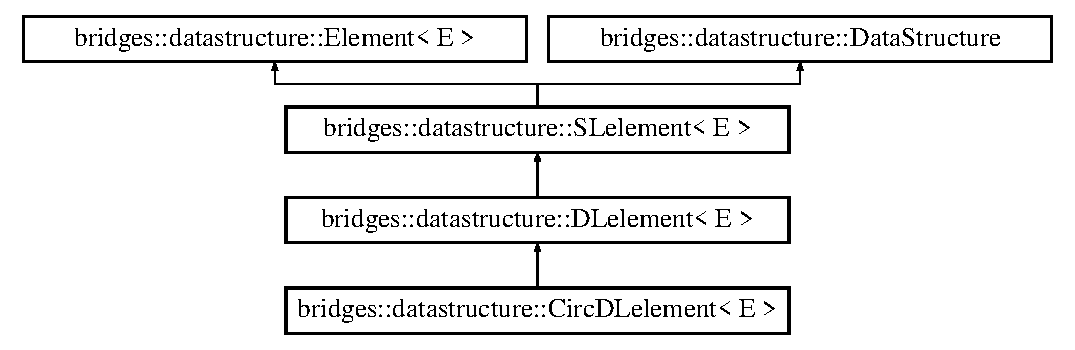
\includegraphics[height=4.000000cm]{classbridges_1_1datastructure_1_1_circ_d_lelement}
\end{center}
\end{figure}


\subsection{Detailed Description}
\subsubsection*{template$<$typename E$>$\newline
class bridges\+::datastructure\+::\+Circ\+D\+Lelement$<$ E $>$}

This class can be used to instantiate Circular Doubly Linked List Elements. 

Structurally they are the same as doubly linked elements except that each node constructed with the next and the previous pointers pointing to itself.

User\textquotesingle{}s implementation of the circularly linked list needs to ensure that the last node\textquotesingle{}s next pointer points to the first node and the first node\textquotesingle{}s previous pointer points to the last node, as the visualization generation is dependent on this.

Elements have labels (string) that are displayed on the visualization. Elements take an generic object E as a user defined parameter, which can any native type or object. Elements contain a visualizer object for setting visual attributes (color, shape, opacity, size), necessary for displaying them in a web browser

\begin{DoxySeeAlso}{See also}
There is a tutorial about Circular Doubly Linked Lists \+: \href{http://bridgesuncc.github.io/tutorials/CircularDoublyLinkedList.html}{\tt http\+://bridgesuncc.\+github.\+io/tutorials/\+Circular\+Doubly\+Linked\+List.\+html}
\end{DoxySeeAlso}
\begin{DoxyAuthor}{Author}
Kalpathi Subramanian 
\end{DoxyAuthor}
\begin{DoxyDate}{Date}
10/5/16, 7/12/19 
\end{DoxyDate}
\subsection*{Classes}
\begin{DoxyCompactItemize}
\item 
class \hyperlink{classbridges_1_1datastructure_1_1_circ_d_lelement_1_1_circ_d_lelement__constlisthelper}{Circ\+D\+Lelement\+\_\+constlisthelper}
\begin{DoxyCompactList}\small\item\em these are helper classes for \hyperlink{classbridges_1_1datastructure_1_1_circ_d_lelement}{Circ\+D\+Lelement} for easy iteration in a range for loop. It is not meant to be created by the bridges user. But it may be returned by \hyperlink{classbridges_1_1_bridges}{Bridges} to provide an S\+TL compliant list A\+PI. \end{DoxyCompactList}\item 
class \hyperlink{classbridges_1_1datastructure_1_1_circ_d_lelement_1_1_circ_d_lelement__listhelper}{Circ\+D\+Lelement\+\_\+listhelper}
\begin{DoxyCompactList}\small\item\em these are helper classes for \hyperlink{classbridges_1_1datastructure_1_1_circ_d_lelement}{Circ\+D\+Lelement} for easy iteration in a range for loop. It is not meant to be created by the bridges user. But it may be returned by \hyperlink{classbridges_1_1_bridges}{Bridges} to provide an S\+TL compliant list A\+PI. \end{DoxyCompactList}\end{DoxyCompactItemize}
\subsection*{Public Member Functions}
\begin{DoxyCompactItemize}
\item 
\hyperlink{classbridges_1_1datastructure_1_1_circ_d_lelement_acd151aff05440f2c6fe26f41b46e0668}{Circ\+D\+Lelement} ()
\item 
\hyperlink{classbridges_1_1datastructure_1_1_circ_d_lelement_a88232de87ec750fccd655d6591870f4c}{Circ\+D\+Lelement} (E e, string label)
\item 
\hyperlink{classbridges_1_1datastructure_1_1_circ_d_lelement_a8db4aa80feb388d5206d657d80385f16}{Circ\+D\+Lelement} (\hyperlink{classbridges_1_1datastructure_1_1_circ_d_lelement}{Circ\+D\+Lelement}$<$ E $>$ \hyperlink{classbridges_1_1datastructure_1_1_s_lelement_afc016a593a4a5aba82021ee34edadbfc}{next}, \hyperlink{classbridges_1_1datastructure_1_1_circ_d_lelement}{Circ\+D\+Lelement}$<$ E $>$ prev)
\item 
\hyperlink{classbridges_1_1datastructure_1_1_circ_d_lelement_a52b304df48ac1ba5a13b4c3c596f433b}{Circ\+D\+Lelement} (E e, \hyperlink{classbridges_1_1datastructure_1_1_circ_d_lelement}{Circ\+D\+Lelement}$<$ E $>$ \hyperlink{classbridges_1_1datastructure_1_1_s_lelement_afc016a593a4a5aba82021ee34edadbfc}{next}, \hyperlink{classbridges_1_1datastructure_1_1_circ_d_lelement}{Circ\+D\+Lelement}$<$ E $>$ prev)
\item 
virtual const string \hyperlink{classbridges_1_1datastructure_1_1_circ_d_lelement_aec7f9b9dc6626c1a872feb91cd65425d}{get\+D\+Stype} () const override
\item 
const \hyperlink{classbridges_1_1datastructure_1_1_circ_d_lelement}{Circ\+D\+Lelement}$<$ E $>$ $\ast$ \hyperlink{classbridges_1_1datastructure_1_1_circ_d_lelement_a3b54f07ffa49151ed13d8b8df964a4ee}{get\+Next} () const override
\item 
virtual \hyperlink{classbridges_1_1datastructure_1_1_circ_d_lelement}{Circ\+D\+Lelement}$<$ E $>$ $\ast$ \hyperlink{classbridges_1_1datastructure_1_1_circ_d_lelement_a80681d0382643a6df21da1bec4067004}{get\+Next} () override
\item 
void \hyperlink{classbridges_1_1datastructure_1_1_circ_d_lelement_aa19f430c7b00a6d38187021255f741e4}{set\+Next} (\hyperlink{classbridges_1_1datastructure_1_1_circ_d_lelement}{Circ\+D\+Lelement}$<$ E $>$ $\ast$\hyperlink{classbridges_1_1datastructure_1_1_s_lelement_afc016a593a4a5aba82021ee34edadbfc}{next})
\item 
\hyperlink{classbridges_1_1datastructure_1_1_circ_d_lelement}{Circ\+D\+Lelement}$<$ E $>$ $\ast$ \hyperlink{classbridges_1_1datastructure_1_1_circ_d_lelement_a5218bb590a588e1d1aaa8f53403ed0cb}{get\+Prev} () override
\item 
const \hyperlink{classbridges_1_1datastructure_1_1_circ_d_lelement}{Circ\+D\+Lelement}$<$ E $>$ $\ast$ \hyperlink{classbridges_1_1datastructure_1_1_circ_d_lelement_a80a08e1d066b1a1f474aa9fd3bc29972}{get\+Prev} () const override
\item 
void \hyperlink{classbridges_1_1datastructure_1_1_circ_d_lelement_ac47b0221a0eebc3c539eec1700f2c776}{set\+Prev} (\hyperlink{classbridges_1_1datastructure_1_1_circ_d_lelement}{Circ\+D\+Lelement}$<$ E $>$ $\ast$prev)
\end{DoxyCompactItemize}
\subsection*{Additional Inherited Members}


\subsection{Constructor \& Destructor Documentation}
\mbox{\Hypertarget{classbridges_1_1datastructure_1_1_circ_d_lelement_acd151aff05440f2c6fe26f41b46e0668}\label{classbridges_1_1datastructure_1_1_circ_d_lelement_acd151aff05440f2c6fe26f41b46e0668}} 
\index{bridges\+::datastructure\+::\+Circ\+D\+Lelement@{bridges\+::datastructure\+::\+Circ\+D\+Lelement}!Circ\+D\+Lelement@{Circ\+D\+Lelement}}
\index{Circ\+D\+Lelement@{Circ\+D\+Lelement}!bridges\+::datastructure\+::\+Circ\+D\+Lelement@{bridges\+::datastructure\+::\+Circ\+D\+Lelement}}
\subsubsection{\texorpdfstring{Circ\+D\+Lelement()}{CircDLelement()}\hspace{0.1cm}{\footnotesize\ttfamily [1/4]}}
{\footnotesize\ttfamily template$<$typename E$>$ \\
\hyperlink{classbridges_1_1datastructure_1_1_circ_d_lelement}{bridges\+::datastructure\+::\+Circ\+D\+Lelement}$<$ E $>$\+::\hyperlink{classbridges_1_1datastructure_1_1_circ_d_lelement}{Circ\+D\+Lelement} (\begin{DoxyParamCaption}{ }\end{DoxyParamCaption})\hspace{0.3cm}{\ttfamily [inline]}}

Constructs an empty \hyperlink{classbridges_1_1datastructure_1_1_circ_d_lelement}{Circ\+D\+Lelement} with next and prev pointers set to itself \mbox{\Hypertarget{classbridges_1_1datastructure_1_1_circ_d_lelement_a88232de87ec750fccd655d6591870f4c}\label{classbridges_1_1datastructure_1_1_circ_d_lelement_a88232de87ec750fccd655d6591870f4c}} 
\index{bridges\+::datastructure\+::\+Circ\+D\+Lelement@{bridges\+::datastructure\+::\+Circ\+D\+Lelement}!Circ\+D\+Lelement@{Circ\+D\+Lelement}}
\index{Circ\+D\+Lelement@{Circ\+D\+Lelement}!bridges\+::datastructure\+::\+Circ\+D\+Lelement@{bridges\+::datastructure\+::\+Circ\+D\+Lelement}}
\subsubsection{\texorpdfstring{Circ\+D\+Lelement()}{CircDLelement()}\hspace{0.1cm}{\footnotesize\ttfamily [2/4]}}
{\footnotesize\ttfamily template$<$typename E$>$ \\
\hyperlink{classbridges_1_1datastructure_1_1_circ_d_lelement}{bridges\+::datastructure\+::\+Circ\+D\+Lelement}$<$ E $>$\+::\hyperlink{classbridges_1_1datastructure_1_1_circ_d_lelement}{Circ\+D\+Lelement} (\begin{DoxyParamCaption}\item[{E}]{e,  }\item[{string}]{label }\end{DoxyParamCaption})\hspace{0.3cm}{\ttfamily [inline]}}

Constructs a \hyperlink{classbridges_1_1datastructure_1_1_circ_d_lelement}{Circ\+D\+Lelement} labeled \char`\"{}label\char`\"{}, holding an object \char`\"{}e\char`\"{}, with next and prev pointers set to itself 
\begin{DoxyParams}{Parameters}
{\em e} & the genereic object that this \hyperlink{classbridges_1_1datastructure_1_1_circ_d_lelement}{Circ\+D\+Lelement} is holding \\
\hline
{\em label} & the label for this \hyperlink{classbridges_1_1datastructure_1_1_circ_d_lelement}{Circ\+D\+Lelement} that shows up on the \hyperlink{classbridges_1_1_bridges}{Bridges} visualization \\
\hline
\end{DoxyParams}
\mbox{\Hypertarget{classbridges_1_1datastructure_1_1_circ_d_lelement_a8db4aa80feb388d5206d657d80385f16}\label{classbridges_1_1datastructure_1_1_circ_d_lelement_a8db4aa80feb388d5206d657d80385f16}} 
\index{bridges\+::datastructure\+::\+Circ\+D\+Lelement@{bridges\+::datastructure\+::\+Circ\+D\+Lelement}!Circ\+D\+Lelement@{Circ\+D\+Lelement}}
\index{Circ\+D\+Lelement@{Circ\+D\+Lelement}!bridges\+::datastructure\+::\+Circ\+D\+Lelement@{bridges\+::datastructure\+::\+Circ\+D\+Lelement}}
\subsubsection{\texorpdfstring{Circ\+D\+Lelement()}{CircDLelement()}\hspace{0.1cm}{\footnotesize\ttfamily [3/4]}}
{\footnotesize\ttfamily template$<$typename E$>$ \\
\hyperlink{classbridges_1_1datastructure_1_1_circ_d_lelement}{bridges\+::datastructure\+::\+Circ\+D\+Lelement}$<$ E $>$\+::\hyperlink{classbridges_1_1datastructure_1_1_circ_d_lelement}{Circ\+D\+Lelement} (\begin{DoxyParamCaption}\item[{\hyperlink{classbridges_1_1datastructure_1_1_circ_d_lelement}{Circ\+D\+Lelement}$<$ E $>$}]{next,  }\item[{\hyperlink{classbridges_1_1datastructure_1_1_circ_d_lelement}{Circ\+D\+Lelement}$<$ E $>$}]{prev }\end{DoxyParamCaption})\hspace{0.3cm}{\ttfamily [inline]}}

Constructs an empty \hyperlink{classbridges_1_1datastructure_1_1_d_lelement}{D\+Lelement} with the next pointer set to the \hyperlink{classbridges_1_1datastructure_1_1_circ_d_lelement}{Circ\+D\+Lelement} \char`\"{}next\char`\"{} and the prev pointer set to \hyperlink{classbridges_1_1datastructure_1_1_circ_d_lelement}{Circ\+D\+Lelement} \char`\"{}prev\char`\"{}.


\begin{DoxyParams}{Parameters}
{\em next} & the \hyperlink{classbridges_1_1datastructure_1_1_d_lelement}{D\+Lelement} that should be assigned to the next pointer \\
\hline
{\em prev} & the \hyperlink{classbridges_1_1datastructure_1_1_d_lelement}{D\+Lelement} that should be assigned to the prev pointer \\
\hline
\end{DoxyParams}
\mbox{\Hypertarget{classbridges_1_1datastructure_1_1_circ_d_lelement_a52b304df48ac1ba5a13b4c3c596f433b}\label{classbridges_1_1datastructure_1_1_circ_d_lelement_a52b304df48ac1ba5a13b4c3c596f433b}} 
\index{bridges\+::datastructure\+::\+Circ\+D\+Lelement@{bridges\+::datastructure\+::\+Circ\+D\+Lelement}!Circ\+D\+Lelement@{Circ\+D\+Lelement}}
\index{Circ\+D\+Lelement@{Circ\+D\+Lelement}!bridges\+::datastructure\+::\+Circ\+D\+Lelement@{bridges\+::datastructure\+::\+Circ\+D\+Lelement}}
\subsubsection{\texorpdfstring{Circ\+D\+Lelement()}{CircDLelement()}\hspace{0.1cm}{\footnotesize\ttfamily [4/4]}}
{\footnotesize\ttfamily template$<$typename E$>$ \\
\hyperlink{classbridges_1_1datastructure_1_1_circ_d_lelement}{bridges\+::datastructure\+::\+Circ\+D\+Lelement}$<$ E $>$\+::\hyperlink{classbridges_1_1datastructure_1_1_circ_d_lelement}{Circ\+D\+Lelement} (\begin{DoxyParamCaption}\item[{E}]{e,  }\item[{\hyperlink{classbridges_1_1datastructure_1_1_circ_d_lelement}{Circ\+D\+Lelement}$<$ E $>$}]{next,  }\item[{\hyperlink{classbridges_1_1datastructure_1_1_circ_d_lelement}{Circ\+D\+Lelement}$<$ E $>$}]{prev }\end{DoxyParamCaption})\hspace{0.3cm}{\ttfamily [inline]}}

Constructs a \hyperlink{classbridges_1_1datastructure_1_1_d_lelement}{D\+Lelement} holding an object \char`\"{}e\char`\"{}, with the next pointer set to the \hyperlink{classbridges_1_1datastructure_1_1_d_lelement}{D\+Lelement} \char`\"{}next\char`\"{} and the prev pointer set to \hyperlink{classbridges_1_1datastructure_1_1_d_lelement}{D\+Lelement} \char`\"{}prev\char`\"{}.


\begin{DoxyParams}{Parameters}
{\em e} & the genereic object that this \hyperlink{classbridges_1_1datastructure_1_1_circ_d_lelement}{Circ\+D\+Lelement} is holding \\
\hline
{\em next} & the \hyperlink{classbridges_1_1datastructure_1_1_circ_d_lelement}{Circ\+D\+Lelement} that should be assigned to the next pointer \\
\hline
{\em prev} & the \hyperlink{classbridges_1_1datastructure_1_1_circ_d_lelement}{Circ\+D\+Lelement} that should be assigned to the prev pointer \\
\hline
\end{DoxyParams}


\subsection{Member Function Documentation}
\mbox{\Hypertarget{classbridges_1_1datastructure_1_1_circ_d_lelement_aec7f9b9dc6626c1a872feb91cd65425d}\label{classbridges_1_1datastructure_1_1_circ_d_lelement_aec7f9b9dc6626c1a872feb91cd65425d}} 
\index{bridges\+::datastructure\+::\+Circ\+D\+Lelement@{bridges\+::datastructure\+::\+Circ\+D\+Lelement}!get\+D\+Stype@{get\+D\+Stype}}
\index{get\+D\+Stype@{get\+D\+Stype}!bridges\+::datastructure\+::\+Circ\+D\+Lelement@{bridges\+::datastructure\+::\+Circ\+D\+Lelement}}
\subsubsection{\texorpdfstring{get\+D\+Stype()}{getDStype()}}
{\footnotesize\ttfamily template$<$typename E$>$ \\
virtual const string \hyperlink{classbridges_1_1datastructure_1_1_circ_d_lelement}{bridges\+::datastructure\+::\+Circ\+D\+Lelement}$<$ E $>$\+::get\+D\+Stype (\begin{DoxyParamCaption}{ }\end{DoxyParamCaption}) const\hspace{0.3cm}{\ttfamily [inline]}, {\ttfamily [override]}, {\ttfamily [virtual]}}

This method gets the data structure type

\begin{DoxyReturn}{Returns}
The date structure type as a string 
\end{DoxyReturn}


Reimplemented from \hyperlink{classbridges_1_1datastructure_1_1_d_lelement_a736ba8e6901608fb0ab04d781d2cceee}{bridges\+::datastructure\+::\+D\+Lelement$<$ E $>$}.

\mbox{\Hypertarget{classbridges_1_1datastructure_1_1_circ_d_lelement_a3b54f07ffa49151ed13d8b8df964a4ee}\label{classbridges_1_1datastructure_1_1_circ_d_lelement_a3b54f07ffa49151ed13d8b8df964a4ee}} 
\index{bridges\+::datastructure\+::\+Circ\+D\+Lelement@{bridges\+::datastructure\+::\+Circ\+D\+Lelement}!get\+Next@{get\+Next}}
\index{get\+Next@{get\+Next}!bridges\+::datastructure\+::\+Circ\+D\+Lelement@{bridges\+::datastructure\+::\+Circ\+D\+Lelement}}
\subsubsection{\texorpdfstring{get\+Next()}{getNext()}\hspace{0.1cm}{\footnotesize\ttfamily [1/2]}}
{\footnotesize\ttfamily template$<$typename E$>$ \\
const \hyperlink{classbridges_1_1datastructure_1_1_circ_d_lelement}{Circ\+D\+Lelement}$<$E$>$$\ast$ \hyperlink{classbridges_1_1datastructure_1_1_circ_d_lelement}{bridges\+::datastructure\+::\+Circ\+D\+Lelement}$<$ E $>$\+::get\+Next (\begin{DoxyParamCaption}{ }\end{DoxyParamCaption}) const\hspace{0.3cm}{\ttfamily [inline]}, {\ttfamily [override]}, {\ttfamily [virtual]}}

This method returns the pointer to the next \hyperlink{classbridges_1_1datastructure_1_1_d_lelement}{D\+Lelement} -\/ const version \begin{DoxyReturn}{Returns}
the \hyperlink{classbridges_1_1datastructure_1_1_d_lelement}{D\+Lelement} assigned to the next pointer 
\end{DoxyReturn}


Reimplemented from \hyperlink{classbridges_1_1datastructure_1_1_d_lelement_a8599e5be5fc1771d4e8a40f6de67b4a7}{bridges\+::datastructure\+::\+D\+Lelement$<$ E $>$}.

\mbox{\Hypertarget{classbridges_1_1datastructure_1_1_circ_d_lelement_a80681d0382643a6df21da1bec4067004}\label{classbridges_1_1datastructure_1_1_circ_d_lelement_a80681d0382643a6df21da1bec4067004}} 
\index{bridges\+::datastructure\+::\+Circ\+D\+Lelement@{bridges\+::datastructure\+::\+Circ\+D\+Lelement}!get\+Next@{get\+Next}}
\index{get\+Next@{get\+Next}!bridges\+::datastructure\+::\+Circ\+D\+Lelement@{bridges\+::datastructure\+::\+Circ\+D\+Lelement}}
\subsubsection{\texorpdfstring{get\+Next()}{getNext()}\hspace{0.1cm}{\footnotesize\ttfamily [2/2]}}
{\footnotesize\ttfamily template$<$typename E$>$ \\
virtual \hyperlink{classbridges_1_1datastructure_1_1_circ_d_lelement}{Circ\+D\+Lelement}$<$E$>$$\ast$ \hyperlink{classbridges_1_1datastructure_1_1_circ_d_lelement}{bridges\+::datastructure\+::\+Circ\+D\+Lelement}$<$ E $>$\+::get\+Next (\begin{DoxyParamCaption}{ }\end{DoxyParamCaption})\hspace{0.3cm}{\ttfamily [inline]}, {\ttfamily [override]}, {\ttfamily [virtual]}}

Retrieves the next \hyperlink{classbridges_1_1datastructure_1_1_circ_s_lelement}{Circ\+S\+Lelement} \begin{DoxyReturn}{Returns}
Circ\+S\+Lelement$<$\+E$>$ assigned to next 
\end{DoxyReturn}


Reimplemented from \hyperlink{classbridges_1_1datastructure_1_1_d_lelement_a63212051ea77d74bd751dea00288d2be}{bridges\+::datastructure\+::\+D\+Lelement$<$ E $>$}.

\mbox{\Hypertarget{classbridges_1_1datastructure_1_1_circ_d_lelement_a5218bb590a588e1d1aaa8f53403ed0cb}\label{classbridges_1_1datastructure_1_1_circ_d_lelement_a5218bb590a588e1d1aaa8f53403ed0cb}} 
\index{bridges\+::datastructure\+::\+Circ\+D\+Lelement@{bridges\+::datastructure\+::\+Circ\+D\+Lelement}!get\+Prev@{get\+Prev}}
\index{get\+Prev@{get\+Prev}!bridges\+::datastructure\+::\+Circ\+D\+Lelement@{bridges\+::datastructure\+::\+Circ\+D\+Lelement}}
\subsubsection{\texorpdfstring{get\+Prev()}{getPrev()}\hspace{0.1cm}{\footnotesize\ttfamily [1/2]}}
{\footnotesize\ttfamily template$<$typename E$>$ \\
\hyperlink{classbridges_1_1datastructure_1_1_circ_d_lelement}{Circ\+D\+Lelement}$<$E$>$$\ast$ \hyperlink{classbridges_1_1datastructure_1_1_circ_d_lelement}{bridges\+::datastructure\+::\+Circ\+D\+Lelement}$<$ E $>$\+::get\+Prev (\begin{DoxyParamCaption}{ }\end{DoxyParamCaption})\hspace{0.3cm}{\ttfamily [inline]}, {\ttfamily [override]}, {\ttfamily [virtual]}}

This method returns the pointer to the previous \hyperlink{classbridges_1_1datastructure_1_1_d_lelement}{D\+Lelement} \begin{DoxyReturn}{Returns}
the \hyperlink{classbridges_1_1datastructure_1_1_d_lelement}{D\+Lelement} assigned to the prev pointer 
\end{DoxyReturn}


Reimplemented from \hyperlink{classbridges_1_1datastructure_1_1_d_lelement_a0edfa823d0fc6f3dba58f85dbf5a11ff}{bridges\+::datastructure\+::\+D\+Lelement$<$ E $>$}.

\mbox{\Hypertarget{classbridges_1_1datastructure_1_1_circ_d_lelement_a80a08e1d066b1a1f474aa9fd3bc29972}\label{classbridges_1_1datastructure_1_1_circ_d_lelement_a80a08e1d066b1a1f474aa9fd3bc29972}} 
\index{bridges\+::datastructure\+::\+Circ\+D\+Lelement@{bridges\+::datastructure\+::\+Circ\+D\+Lelement}!get\+Prev@{get\+Prev}}
\index{get\+Prev@{get\+Prev}!bridges\+::datastructure\+::\+Circ\+D\+Lelement@{bridges\+::datastructure\+::\+Circ\+D\+Lelement}}
\subsubsection{\texorpdfstring{get\+Prev()}{getPrev()}\hspace{0.1cm}{\footnotesize\ttfamily [2/2]}}
{\footnotesize\ttfamily template$<$typename E$>$ \\
const \hyperlink{classbridges_1_1datastructure_1_1_circ_d_lelement}{Circ\+D\+Lelement}$<$E$>$$\ast$ \hyperlink{classbridges_1_1datastructure_1_1_circ_d_lelement}{bridges\+::datastructure\+::\+Circ\+D\+Lelement}$<$ E $>$\+::get\+Prev (\begin{DoxyParamCaption}{ }\end{DoxyParamCaption}) const\hspace{0.3cm}{\ttfamily [inline]}, {\ttfamily [override]}, {\ttfamily [virtual]}}

This method returns the pointer to the previous \hyperlink{classbridges_1_1datastructure_1_1_d_lelement}{D\+Lelement} \begin{DoxyReturn}{Returns}
the \hyperlink{classbridges_1_1datastructure_1_1_d_lelement}{D\+Lelement} assigned to the prev pointer 
\end{DoxyReturn}


Reimplemented from \hyperlink{classbridges_1_1datastructure_1_1_d_lelement_a66917ba9a9270b8f6b5e4ff258bf3e70}{bridges\+::datastructure\+::\+D\+Lelement$<$ E $>$}.

\mbox{\Hypertarget{classbridges_1_1datastructure_1_1_circ_d_lelement_aa19f430c7b00a6d38187021255f741e4}\label{classbridges_1_1datastructure_1_1_circ_d_lelement_aa19f430c7b00a6d38187021255f741e4}} 
\index{bridges\+::datastructure\+::\+Circ\+D\+Lelement@{bridges\+::datastructure\+::\+Circ\+D\+Lelement}!set\+Next@{set\+Next}}
\index{set\+Next@{set\+Next}!bridges\+::datastructure\+::\+Circ\+D\+Lelement@{bridges\+::datastructure\+::\+Circ\+D\+Lelement}}
\subsubsection{\texorpdfstring{set\+Next()}{setNext()}}
{\footnotesize\ttfamily template$<$typename E$>$ \\
void \hyperlink{classbridges_1_1datastructure_1_1_circ_d_lelement}{bridges\+::datastructure\+::\+Circ\+D\+Lelement}$<$ E $>$\+::set\+Next (\begin{DoxyParamCaption}\item[{\hyperlink{classbridges_1_1datastructure_1_1_circ_d_lelement}{Circ\+D\+Lelement}$<$ E $>$ $\ast$}]{next }\end{DoxyParamCaption})\hspace{0.3cm}{\ttfamily [inline]}}

This method sets the pointer to the next \hyperlink{classbridges_1_1datastructure_1_1_d_lelement}{D\+Lelement}


\begin{DoxyParams}{Parameters}
{\em next} & the \hyperlink{classbridges_1_1datastructure_1_1_d_lelement}{D\+Lelement} that should be assigned to the next pointer \\
\hline
\end{DoxyParams}
\mbox{\Hypertarget{classbridges_1_1datastructure_1_1_circ_d_lelement_ac47b0221a0eebc3c539eec1700f2c776}\label{classbridges_1_1datastructure_1_1_circ_d_lelement_ac47b0221a0eebc3c539eec1700f2c776}} 
\index{bridges\+::datastructure\+::\+Circ\+D\+Lelement@{bridges\+::datastructure\+::\+Circ\+D\+Lelement}!set\+Prev@{set\+Prev}}
\index{set\+Prev@{set\+Prev}!bridges\+::datastructure\+::\+Circ\+D\+Lelement@{bridges\+::datastructure\+::\+Circ\+D\+Lelement}}
\subsubsection{\texorpdfstring{set\+Prev()}{setPrev()}}
{\footnotesize\ttfamily template$<$typename E$>$ \\
void \hyperlink{classbridges_1_1datastructure_1_1_circ_d_lelement}{bridges\+::datastructure\+::\+Circ\+D\+Lelement}$<$ E $>$\+::set\+Prev (\begin{DoxyParamCaption}\item[{\hyperlink{classbridges_1_1datastructure_1_1_circ_d_lelement}{Circ\+D\+Lelement}$<$ E $>$ $\ast$}]{prev }\end{DoxyParamCaption})\hspace{0.3cm}{\ttfamily [inline]}}

This method sets the pointer to the previous \hyperlink{classbridges_1_1datastructure_1_1_d_lelement}{D\+Lelement} 
\begin{DoxyParams}{Parameters}
{\em prev} & the \hyperlink{classbridges_1_1datastructure_1_1_d_lelement}{D\+Lelement} that should be assigned to the prev pointer \\
\hline
\end{DoxyParams}


The documentation for this class was generated from the following file\+:\begin{DoxyCompactItemize}
\item 
/home/erik/work/bridges/bridges-\/cxx/src/\hyperlink{_circ_d_lelement_8h}{Circ\+D\+Lelement.\+h}\end{DoxyCompactItemize}

\hypertarget{classbridges_1_1datastructure_1_1_circ_d_lelement_1_1_circ_d_lelement__constlisthelper}{}\doxysection{bridges\+::datastructure\+::Circ\+DLelement$<$ E $>$\+::Circ\+DLelement\+\_\+constlisthelper Class Reference}
\label{classbridges_1_1datastructure_1_1_circ_d_lelement_1_1_circ_d_lelement__constlisthelper}\index{bridges::datastructure::CircDLelement$<$ E $>$::CircDLelement\_constlisthelper@{bridges::datastructure::CircDLelement$<$ E $>$::CircDLelement\_constlisthelper}}


{\ttfamily \#include $<$Circ\+DLelement.\+h$>$}



\doxysubsection{Detailed Description}
\subsubsection*{template$<$typename E$>$\newline
class bridges\+::datastructure\+::\+Circ\+DLelement$<$ E $>$\+::\+Circ\+DLelement\+\_\+constlisthelper}

these are helper classes for \mbox{\hyperlink{classbridges_1_1datastructure_1_1_circ_d_lelement}{Circ\+DLelement}} for easy iteration in a range for loop. It is not meant to be created by the bridges user. But it may be returned by \mbox{\hyperlink{classbridges_1_1_bridges}{Bridges}} to provide an STL compliant list API. \doxysubsection*{Classes}
\begin{DoxyCompactItemize}
\item 
class \mbox{\hyperlink{classbridges_1_1datastructure_1_1_circ_d_lelement_1_1_circ_d_lelement__constlisthelper_1_1iterator}{iterator}}
\end{DoxyCompactItemize}
\doxysubsection*{Public Member Functions}
\begin{DoxyCompactItemize}
\item 
\mbox{\hyperlink{classbridges_1_1datastructure_1_1_circ_d_lelement_1_1_circ_d_lelement__constlisthelper_acb75735d01573db3b99f81632aae490c}{Circ\+DLelement\+\_\+constlisthelper}} (typename \mbox{\hyperlink{classbridges_1_1datastructure_1_1_circ_d_lelement}{bridges\+::datastructure\+::\+Circ\+DLelement}}$<$ E $>$ const $\ast$s)
\item 
\mbox{\hyperlink{classbridges_1_1datastructure_1_1_circ_d_lelement_1_1_circ_d_lelement__constlisthelper_1_1iterator}{iterator}} \mbox{\hyperlink{classbridges_1_1datastructure_1_1_circ_d_lelement_1_1_circ_d_lelement__constlisthelper_a3c0505dae6b044cbb0c56c772eb33b3e}{begin}} ()
\item 
\mbox{\hyperlink{classbridges_1_1datastructure_1_1_circ_d_lelement_1_1_circ_d_lelement__constlisthelper_1_1iterator}{iterator}} \mbox{\hyperlink{classbridges_1_1datastructure_1_1_circ_d_lelement_1_1_circ_d_lelement__constlisthelper_ac6c3b1a138ae5c8ddb0b55d08c4ae19d}{end}} ()
\item 
\mbox{\hyperlink{classbridges_1_1datastructure_1_1_circ_d_lelement_1_1_circ_d_lelement__constlisthelper_1_1iterator}{iterator}} \mbox{\hyperlink{classbridges_1_1datastructure_1_1_circ_d_lelement_1_1_circ_d_lelement__constlisthelper_abf94a30d0eeddd99752fd2dfca86665d}{rbegin}} ()
\item 
\mbox{\hyperlink{classbridges_1_1datastructure_1_1_circ_d_lelement_1_1_circ_d_lelement__constlisthelper_1_1iterator}{iterator}} \mbox{\hyperlink{classbridges_1_1datastructure_1_1_circ_d_lelement_1_1_circ_d_lelement__constlisthelper_adcfb956dad9f130975df6632f97a3b82}{rend}} ()
\end{DoxyCompactItemize}


\doxysubsection{Constructor \& Destructor Documentation}
\mbox{\Hypertarget{classbridges_1_1datastructure_1_1_circ_d_lelement_1_1_circ_d_lelement__constlisthelper_acb75735d01573db3b99f81632aae490c}\label{classbridges_1_1datastructure_1_1_circ_d_lelement_1_1_circ_d_lelement__constlisthelper_acb75735d01573db3b99f81632aae490c}} 
\index{bridges::datastructure::CircDLelement$<$ E $>$::CircDLelement\_constlisthelper@{bridges::datastructure::CircDLelement$<$ E $>$::CircDLelement\_constlisthelper}!CircDLelement\_constlisthelper@{CircDLelement\_constlisthelper}}
\index{CircDLelement\_constlisthelper@{CircDLelement\_constlisthelper}!bridges::datastructure::CircDLelement$<$ E $>$::CircDLelement\_constlisthelper@{bridges::datastructure::CircDLelement$<$ E $>$::CircDLelement\_constlisthelper}}
\doxysubsubsection{\texorpdfstring{CircDLelement\_constlisthelper()}{CircDLelement\_constlisthelper()}}
{\footnotesize\ttfamily template$<$typename E $>$ \\
\mbox{\hyperlink{classbridges_1_1datastructure_1_1_circ_d_lelement}{bridges\+::datastructure\+::\+Circ\+DLelement}}$<$ E $>$\+::Circ\+DLelement\+\_\+constlisthelper\+::\+Circ\+DLelement\+\_\+constlisthelper (\begin{DoxyParamCaption}\item[{typename \mbox{\hyperlink{classbridges_1_1datastructure_1_1_circ_d_lelement}{bridges\+::datastructure\+::\+Circ\+DLelement}}$<$ E $>$ const $\ast$}]{s }\end{DoxyParamCaption})\hspace{0.3cm}{\ttfamily [inline]}}



\doxysubsection{Member Function Documentation}
\mbox{\Hypertarget{classbridges_1_1datastructure_1_1_circ_d_lelement_1_1_circ_d_lelement__constlisthelper_a3c0505dae6b044cbb0c56c772eb33b3e}\label{classbridges_1_1datastructure_1_1_circ_d_lelement_1_1_circ_d_lelement__constlisthelper_a3c0505dae6b044cbb0c56c772eb33b3e}} 
\index{bridges::datastructure::CircDLelement$<$ E $>$::CircDLelement\_constlisthelper@{bridges::datastructure::CircDLelement$<$ E $>$::CircDLelement\_constlisthelper}!begin@{begin}}
\index{begin@{begin}!bridges::datastructure::CircDLelement$<$ E $>$::CircDLelement\_constlisthelper@{bridges::datastructure::CircDLelement$<$ E $>$::CircDLelement\_constlisthelper}}
\doxysubsubsection{\texorpdfstring{begin()}{begin()}}
{\footnotesize\ttfamily template$<$typename E $>$ \\
\mbox{\hyperlink{classbridges_1_1datastructure_1_1_circ_d_lelement_1_1_circ_d_lelement__constlisthelper_1_1iterator}{iterator}} \mbox{\hyperlink{classbridges_1_1datastructure_1_1_circ_d_lelement}{bridges\+::datastructure\+::\+Circ\+DLelement}}$<$ E $>$\+::Circ\+DLelement\+\_\+constlisthelper\+::begin (\begin{DoxyParamCaption}{ }\end{DoxyParamCaption})\hspace{0.3cm}{\ttfamily [inline]}}

\mbox{\Hypertarget{classbridges_1_1datastructure_1_1_circ_d_lelement_1_1_circ_d_lelement__constlisthelper_ac6c3b1a138ae5c8ddb0b55d08c4ae19d}\label{classbridges_1_1datastructure_1_1_circ_d_lelement_1_1_circ_d_lelement__constlisthelper_ac6c3b1a138ae5c8ddb0b55d08c4ae19d}} 
\index{bridges::datastructure::CircDLelement$<$ E $>$::CircDLelement\_constlisthelper@{bridges::datastructure::CircDLelement$<$ E $>$::CircDLelement\_constlisthelper}!end@{end}}
\index{end@{end}!bridges::datastructure::CircDLelement$<$ E $>$::CircDLelement\_constlisthelper@{bridges::datastructure::CircDLelement$<$ E $>$::CircDLelement\_constlisthelper}}
\doxysubsubsection{\texorpdfstring{end()}{end()}}
{\footnotesize\ttfamily template$<$typename E $>$ \\
\mbox{\hyperlink{classbridges_1_1datastructure_1_1_circ_d_lelement_1_1_circ_d_lelement__constlisthelper_1_1iterator}{iterator}} \mbox{\hyperlink{classbridges_1_1datastructure_1_1_circ_d_lelement}{bridges\+::datastructure\+::\+Circ\+DLelement}}$<$ E $>$\+::Circ\+DLelement\+\_\+constlisthelper\+::end (\begin{DoxyParamCaption}{ }\end{DoxyParamCaption})\hspace{0.3cm}{\ttfamily [inline]}}

\mbox{\Hypertarget{classbridges_1_1datastructure_1_1_circ_d_lelement_1_1_circ_d_lelement__constlisthelper_abf94a30d0eeddd99752fd2dfca86665d}\label{classbridges_1_1datastructure_1_1_circ_d_lelement_1_1_circ_d_lelement__constlisthelper_abf94a30d0eeddd99752fd2dfca86665d}} 
\index{bridges::datastructure::CircDLelement$<$ E $>$::CircDLelement\_constlisthelper@{bridges::datastructure::CircDLelement$<$ E $>$::CircDLelement\_constlisthelper}!rbegin@{rbegin}}
\index{rbegin@{rbegin}!bridges::datastructure::CircDLelement$<$ E $>$::CircDLelement\_constlisthelper@{bridges::datastructure::CircDLelement$<$ E $>$::CircDLelement\_constlisthelper}}
\doxysubsubsection{\texorpdfstring{rbegin()}{rbegin()}}
{\footnotesize\ttfamily template$<$typename E $>$ \\
\mbox{\hyperlink{classbridges_1_1datastructure_1_1_circ_d_lelement_1_1_circ_d_lelement__constlisthelper_1_1iterator}{iterator}} \mbox{\hyperlink{classbridges_1_1datastructure_1_1_circ_d_lelement}{bridges\+::datastructure\+::\+Circ\+DLelement}}$<$ E $>$\+::Circ\+DLelement\+\_\+constlisthelper\+::rbegin (\begin{DoxyParamCaption}{ }\end{DoxyParamCaption})\hspace{0.3cm}{\ttfamily [inline]}}

\mbox{\Hypertarget{classbridges_1_1datastructure_1_1_circ_d_lelement_1_1_circ_d_lelement__constlisthelper_adcfb956dad9f130975df6632f97a3b82}\label{classbridges_1_1datastructure_1_1_circ_d_lelement_1_1_circ_d_lelement__constlisthelper_adcfb956dad9f130975df6632f97a3b82}} 
\index{bridges::datastructure::CircDLelement$<$ E $>$::CircDLelement\_constlisthelper@{bridges::datastructure::CircDLelement$<$ E $>$::CircDLelement\_constlisthelper}!rend@{rend}}
\index{rend@{rend}!bridges::datastructure::CircDLelement$<$ E $>$::CircDLelement\_constlisthelper@{bridges::datastructure::CircDLelement$<$ E $>$::CircDLelement\_constlisthelper}}
\doxysubsubsection{\texorpdfstring{rend()}{rend()}}
{\footnotesize\ttfamily template$<$typename E $>$ \\
\mbox{\hyperlink{classbridges_1_1datastructure_1_1_circ_d_lelement_1_1_circ_d_lelement__constlisthelper_1_1iterator}{iterator}} \mbox{\hyperlink{classbridges_1_1datastructure_1_1_circ_d_lelement}{bridges\+::datastructure\+::\+Circ\+DLelement}}$<$ E $>$\+::Circ\+DLelement\+\_\+constlisthelper\+::rend (\begin{DoxyParamCaption}{ }\end{DoxyParamCaption})\hspace{0.3cm}{\ttfamily [inline]}}



The documentation for this class was generated from the following file\+:\begin{DoxyCompactItemize}
\item 
/home/erik/work/bridges/bridges-\/cxx/src/\mbox{\hyperlink{_circ_d_lelement_8h}{Circ\+DLelement.\+h}}\end{DoxyCompactItemize}

\hypertarget{classbridges_1_1datastructure_1_1_circ_d_lelement_1_1_circ_d_lelement__listhelper}{}\doxysection{bridges\+::datastructure\+::Circ\+DLelement$<$ E $>$\+::Circ\+DLelement\+\_\+listhelper Class Reference}
\label{classbridges_1_1datastructure_1_1_circ_d_lelement_1_1_circ_d_lelement__listhelper}\index{bridges::datastructure::CircDLelement$<$ E $>$::CircDLelement\_listhelper@{bridges::datastructure::CircDLelement$<$ E $>$::CircDLelement\_listhelper}}


{\ttfamily \#include $<$Circ\+DLelement.\+h$>$}



\doxysubsection{Detailed Description}
\subsubsection*{template$<$typename E$>$\newline
class bridges\+::datastructure\+::\+Circ\+DLelement$<$ E $>$\+::\+Circ\+DLelement\+\_\+listhelper}

these are helper classes for \mbox{\hyperlink{classbridges_1_1datastructure_1_1_circ_d_lelement}{Circ\+DLelement}} for easy iteration in a range for loop. It is not meant to be created by the bridges user. But it may be returned by \mbox{\hyperlink{classbridges_1_1_bridges}{Bridges}} to provide an STL compliant list API. \doxysubsection*{Classes}
\begin{DoxyCompactItemize}
\item 
class \mbox{\hyperlink{classbridges_1_1datastructure_1_1_circ_d_lelement_1_1_circ_d_lelement__listhelper_1_1iterator}{iterator}}
\end{DoxyCompactItemize}
\doxysubsection*{Public Member Functions}
\begin{DoxyCompactItemize}
\item 
\mbox{\hyperlink{classbridges_1_1datastructure_1_1_circ_d_lelement_1_1_circ_d_lelement__listhelper_a3818959b579e2c397721cb7379b183b2}{Circ\+DLelement\+\_\+listhelper}} (typename \mbox{\hyperlink{classbridges_1_1datastructure_1_1_circ_d_lelement}{bridges\+::datastructure\+::\+Circ\+DLelement}}$<$ E $>$ $\ast$s)
\item 
\mbox{\hyperlink{classbridges_1_1datastructure_1_1_circ_d_lelement_1_1_circ_d_lelement__listhelper_1_1iterator}{iterator}} \mbox{\hyperlink{classbridges_1_1datastructure_1_1_circ_d_lelement_1_1_circ_d_lelement__listhelper_a41cd9455769e78983c62de22d4a6925c}{begin}} ()
\item 
\mbox{\hyperlink{classbridges_1_1datastructure_1_1_circ_d_lelement_1_1_circ_d_lelement__listhelper_1_1iterator}{iterator}} \mbox{\hyperlink{classbridges_1_1datastructure_1_1_circ_d_lelement_1_1_circ_d_lelement__listhelper_a822b5a9427e017cb2363d681a78e3c70}{end}} ()
\item 
\mbox{\hyperlink{classbridges_1_1datastructure_1_1_circ_d_lelement_1_1_circ_d_lelement__listhelper_1_1iterator}{iterator}} \mbox{\hyperlink{classbridges_1_1datastructure_1_1_circ_d_lelement_1_1_circ_d_lelement__listhelper_aec74a9bcb91e1c12367d6ff82c64633e}{rbegin}} ()
\item 
\mbox{\hyperlink{classbridges_1_1datastructure_1_1_circ_d_lelement_1_1_circ_d_lelement__listhelper_1_1iterator}{iterator}} \mbox{\hyperlink{classbridges_1_1datastructure_1_1_circ_d_lelement_1_1_circ_d_lelement__listhelper_a0d26c54b82fcd733dcb445e0c39dc28e}{rend}} ()
\end{DoxyCompactItemize}


\doxysubsection{Constructor \& Destructor Documentation}
\mbox{\Hypertarget{classbridges_1_1datastructure_1_1_circ_d_lelement_1_1_circ_d_lelement__listhelper_a3818959b579e2c397721cb7379b183b2}\label{classbridges_1_1datastructure_1_1_circ_d_lelement_1_1_circ_d_lelement__listhelper_a3818959b579e2c397721cb7379b183b2}} 
\index{bridges::datastructure::CircDLelement$<$ E $>$::CircDLelement\_listhelper@{bridges::datastructure::CircDLelement$<$ E $>$::CircDLelement\_listhelper}!CircDLelement\_listhelper@{CircDLelement\_listhelper}}
\index{CircDLelement\_listhelper@{CircDLelement\_listhelper}!bridges::datastructure::CircDLelement$<$ E $>$::CircDLelement\_listhelper@{bridges::datastructure::CircDLelement$<$ E $>$::CircDLelement\_listhelper}}
\doxysubsubsection{\texorpdfstring{CircDLelement\_listhelper()}{CircDLelement\_listhelper()}}
{\footnotesize\ttfamily template$<$typename E $>$ \\
\mbox{\hyperlink{classbridges_1_1datastructure_1_1_circ_d_lelement}{bridges\+::datastructure\+::\+Circ\+DLelement}}$<$ E $>$\+::Circ\+DLelement\+\_\+listhelper\+::\+Circ\+DLelement\+\_\+listhelper (\begin{DoxyParamCaption}\item[{typename \mbox{\hyperlink{classbridges_1_1datastructure_1_1_circ_d_lelement}{bridges\+::datastructure\+::\+Circ\+DLelement}}$<$ E $>$ $\ast$}]{s }\end{DoxyParamCaption})\hspace{0.3cm}{\ttfamily [inline]}}



\doxysubsection{Member Function Documentation}
\mbox{\Hypertarget{classbridges_1_1datastructure_1_1_circ_d_lelement_1_1_circ_d_lelement__listhelper_a41cd9455769e78983c62de22d4a6925c}\label{classbridges_1_1datastructure_1_1_circ_d_lelement_1_1_circ_d_lelement__listhelper_a41cd9455769e78983c62de22d4a6925c}} 
\index{bridges::datastructure::CircDLelement$<$ E $>$::CircDLelement\_listhelper@{bridges::datastructure::CircDLelement$<$ E $>$::CircDLelement\_listhelper}!begin@{begin}}
\index{begin@{begin}!bridges::datastructure::CircDLelement$<$ E $>$::CircDLelement\_listhelper@{bridges::datastructure::CircDLelement$<$ E $>$::CircDLelement\_listhelper}}
\doxysubsubsection{\texorpdfstring{begin()}{begin()}}
{\footnotesize\ttfamily template$<$typename E $>$ \\
\mbox{\hyperlink{classbridges_1_1datastructure_1_1_circ_d_lelement_1_1_circ_d_lelement__listhelper_1_1iterator}{iterator}} \mbox{\hyperlink{classbridges_1_1datastructure_1_1_circ_d_lelement}{bridges\+::datastructure\+::\+Circ\+DLelement}}$<$ E $>$\+::Circ\+DLelement\+\_\+listhelper\+::begin (\begin{DoxyParamCaption}{ }\end{DoxyParamCaption})\hspace{0.3cm}{\ttfamily [inline]}}

\mbox{\Hypertarget{classbridges_1_1datastructure_1_1_circ_d_lelement_1_1_circ_d_lelement__listhelper_a822b5a9427e017cb2363d681a78e3c70}\label{classbridges_1_1datastructure_1_1_circ_d_lelement_1_1_circ_d_lelement__listhelper_a822b5a9427e017cb2363d681a78e3c70}} 
\index{bridges::datastructure::CircDLelement$<$ E $>$::CircDLelement\_listhelper@{bridges::datastructure::CircDLelement$<$ E $>$::CircDLelement\_listhelper}!end@{end}}
\index{end@{end}!bridges::datastructure::CircDLelement$<$ E $>$::CircDLelement\_listhelper@{bridges::datastructure::CircDLelement$<$ E $>$::CircDLelement\_listhelper}}
\doxysubsubsection{\texorpdfstring{end()}{end()}}
{\footnotesize\ttfamily template$<$typename E $>$ \\
\mbox{\hyperlink{classbridges_1_1datastructure_1_1_circ_d_lelement_1_1_circ_d_lelement__listhelper_1_1iterator}{iterator}} \mbox{\hyperlink{classbridges_1_1datastructure_1_1_circ_d_lelement}{bridges\+::datastructure\+::\+Circ\+DLelement}}$<$ E $>$\+::Circ\+DLelement\+\_\+listhelper\+::end (\begin{DoxyParamCaption}{ }\end{DoxyParamCaption})\hspace{0.3cm}{\ttfamily [inline]}}

\mbox{\Hypertarget{classbridges_1_1datastructure_1_1_circ_d_lelement_1_1_circ_d_lelement__listhelper_aec74a9bcb91e1c12367d6ff82c64633e}\label{classbridges_1_1datastructure_1_1_circ_d_lelement_1_1_circ_d_lelement__listhelper_aec74a9bcb91e1c12367d6ff82c64633e}} 
\index{bridges::datastructure::CircDLelement$<$ E $>$::CircDLelement\_listhelper@{bridges::datastructure::CircDLelement$<$ E $>$::CircDLelement\_listhelper}!rbegin@{rbegin}}
\index{rbegin@{rbegin}!bridges::datastructure::CircDLelement$<$ E $>$::CircDLelement\_listhelper@{bridges::datastructure::CircDLelement$<$ E $>$::CircDLelement\_listhelper}}
\doxysubsubsection{\texorpdfstring{rbegin()}{rbegin()}}
{\footnotesize\ttfamily template$<$typename E $>$ \\
\mbox{\hyperlink{classbridges_1_1datastructure_1_1_circ_d_lelement_1_1_circ_d_lelement__listhelper_1_1iterator}{iterator}} \mbox{\hyperlink{classbridges_1_1datastructure_1_1_circ_d_lelement}{bridges\+::datastructure\+::\+Circ\+DLelement}}$<$ E $>$\+::Circ\+DLelement\+\_\+listhelper\+::rbegin (\begin{DoxyParamCaption}{ }\end{DoxyParamCaption})\hspace{0.3cm}{\ttfamily [inline]}}

\mbox{\Hypertarget{classbridges_1_1datastructure_1_1_circ_d_lelement_1_1_circ_d_lelement__listhelper_a0d26c54b82fcd733dcb445e0c39dc28e}\label{classbridges_1_1datastructure_1_1_circ_d_lelement_1_1_circ_d_lelement__listhelper_a0d26c54b82fcd733dcb445e0c39dc28e}} 
\index{bridges::datastructure::CircDLelement$<$ E $>$::CircDLelement\_listhelper@{bridges::datastructure::CircDLelement$<$ E $>$::CircDLelement\_listhelper}!rend@{rend}}
\index{rend@{rend}!bridges::datastructure::CircDLelement$<$ E $>$::CircDLelement\_listhelper@{bridges::datastructure::CircDLelement$<$ E $>$::CircDLelement\_listhelper}}
\doxysubsubsection{\texorpdfstring{rend()}{rend()}}
{\footnotesize\ttfamily template$<$typename E $>$ \\
\mbox{\hyperlink{classbridges_1_1datastructure_1_1_circ_d_lelement_1_1_circ_d_lelement__listhelper_1_1iterator}{iterator}} \mbox{\hyperlink{classbridges_1_1datastructure_1_1_circ_d_lelement}{bridges\+::datastructure\+::\+Circ\+DLelement}}$<$ E $>$\+::Circ\+DLelement\+\_\+listhelper\+::rend (\begin{DoxyParamCaption}{ }\end{DoxyParamCaption})\hspace{0.3cm}{\ttfamily [inline]}}



The documentation for this class was generated from the following file\+:\begin{DoxyCompactItemize}
\item 
/home/erik/work/bridges/bridges-\/cxx/src/\mbox{\hyperlink{_circ_d_lelement_8h}{Circ\+DLelement.\+h}}\end{DoxyCompactItemize}

\hypertarget{classbridges_1_1datastructure_1_1_circle}{}\section{bridges\+:\+:datastructure\+:\+:Circle Class Reference}
\label{classbridges_1_1datastructure_1_1_circle}\index{bridges\+::datastructure\+::\+Circle@{bridges\+::datastructure\+::\+Circle}}


{\ttfamily \#include $<$Circle.\+h$>$}

Inheritance diagram for bridges\+:\+:datastructure\+:\+:Circle\+:\begin{figure}[H]
\begin{center}
\leavevmode
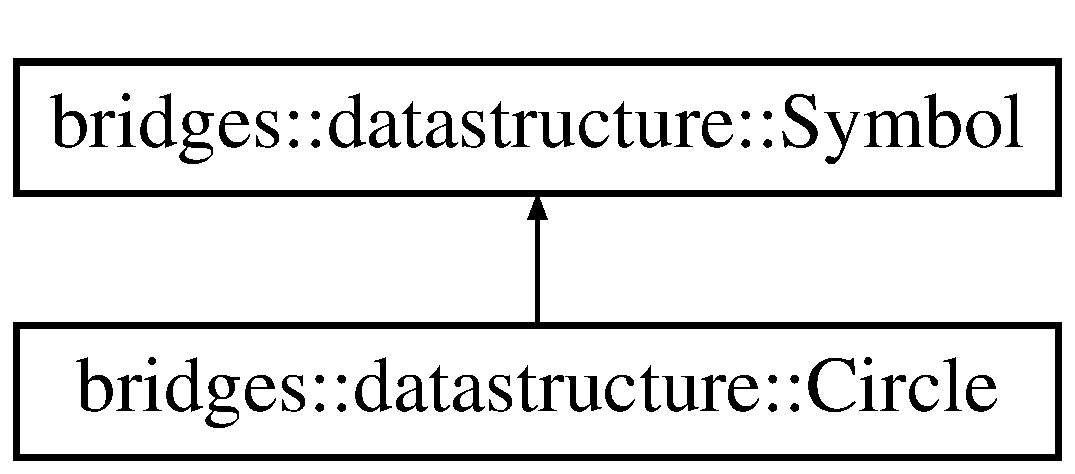
\includegraphics[height=2.000000cm]{classbridges_1_1datastructure_1_1_circle}
\end{center}
\end{figure}


\subsection{Detailed Description}
This class defines a circle and is part of the symbol collection. A circle has a radius. 

\begin{DoxyAuthor}{Author}
Kalpathi Subramanian 
\end{DoxyAuthor}
\begin{DoxyDate}{Date}
12/24/18, 7/12/19 
\end{DoxyDate}
\subsection*{Public Member Functions}
\begin{DoxyCompactItemize}
\item 
\mbox{\hyperlink{classbridges_1_1datastructure_1_1_circle_a2106fef85f001fbd2de2d9870a432ef8}{Circle}} ()
\item 
\mbox{\hyperlink{classbridges_1_1datastructure_1_1_circle_aafbf518a6d7defa3d69d46d4bdda41da}{Circle}} (int r)
\item 
\mbox{\hyperlink{classbridges_1_1datastructure_1_1_circle_acde4da631bd56847058a29f03417ea4e}{Circle}} (int locx, int locy, int r)
\item 
string \mbox{\hyperlink{classbridges_1_1datastructure_1_1_circle_a366d6a7488f926c1d63d6480fc52e791}{get\+Data\+Struct\+Type}} ()
\item 
string \mbox{\hyperlink{classbridges_1_1datastructure_1_1_circle_a3c7808f7918cb01ceaa3f6bf46e6bee5}{get\+Name}} () const
\item 
void \mbox{\hyperlink{classbridges_1_1datastructure_1_1_circle_a5b93bf688d56c7781390e6f207501313}{set\+Radius}} (int r)
\begin{DoxyCompactList}\small\item\em This method sets the radius of the circle. \end{DoxyCompactList}\item 
void \mbox{\hyperlink{classbridges_1_1datastructure_1_1_circle_ab9a1f6a9b76bb4e19b7f5c3e19a0f37f}{set\+Circle}} (int locx, int locy, int r)
\begin{DoxyCompactList}\small\item\em This method sets the circle dimensions. \end{DoxyCompactList}\item 
void \mbox{\hyperlink{classbridges_1_1datastructure_1_1_circle_ac21454141030b7c5af288ddbe2028111}{translate}} (float tx, float ty)
\begin{DoxyCompactList}\small\item\em Translate the circle. \end{DoxyCompactList}\item 
void \mbox{\hyperlink{classbridges_1_1datastructure_1_1_circle_a77c35a4e0a69f8ba1b71c0c40c727eab}{scale}} (float scale)
\item 
vector$<$ float $>$ \mbox{\hyperlink{classbridges_1_1datastructure_1_1_circle_a4e08c866e2f10945c16921454d49a030}{get\+Dimensions}} ()
\item 
const string \mbox{\hyperlink{classbridges_1_1datastructure_1_1_circle_a796c88ccb8c5529d45aa7271a34fa3fe}{get\+Symbol\+Representation}} () const
\end{DoxyCompactItemize}
\subsection*{Additional Inherited Members}


\subsection{Constructor \& Destructor Documentation}
\mbox{\Hypertarget{classbridges_1_1datastructure_1_1_circle_a2106fef85f001fbd2de2d9870a432ef8}\label{classbridges_1_1datastructure_1_1_circle_a2106fef85f001fbd2de2d9870a432ef8}} 
\index{bridges\+::datastructure\+::\+Circle@{bridges\+::datastructure\+::\+Circle}!Circle@{Circle}}
\index{Circle@{Circle}!bridges\+::datastructure\+::\+Circle@{bridges\+::datastructure\+::\+Circle}}
\subsubsection{\texorpdfstring{Circle()}{Circle()}\hspace{0.1cm}{\footnotesize\ttfamily [1/3]}}
{\footnotesize\ttfamily bridges\+::datastructure\+::\+Circle\+::\+Circle (\begin{DoxyParamCaption}{ }\end{DoxyParamCaption})\hspace{0.3cm}{\ttfamily [inline]}}

constructors \mbox{\Hypertarget{classbridges_1_1datastructure_1_1_circle_aafbf518a6d7defa3d69d46d4bdda41da}\label{classbridges_1_1datastructure_1_1_circle_aafbf518a6d7defa3d69d46d4bdda41da}} 
\index{bridges\+::datastructure\+::\+Circle@{bridges\+::datastructure\+::\+Circle}!Circle@{Circle}}
\index{Circle@{Circle}!bridges\+::datastructure\+::\+Circle@{bridges\+::datastructure\+::\+Circle}}
\subsubsection{\texorpdfstring{Circle()}{Circle()}\hspace{0.1cm}{\footnotesize\ttfamily [2/3]}}
{\footnotesize\ttfamily bridges\+::datastructure\+::\+Circle\+::\+Circle (\begin{DoxyParamCaption}\item[{int}]{r }\end{DoxyParamCaption})\hspace{0.3cm}{\ttfamily [inline]}}

Create a circle of radius r 
\begin{DoxyParams}{Parameters}
{\em r} & \+: radius \\
\hline
\end{DoxyParams}
\mbox{\Hypertarget{classbridges_1_1datastructure_1_1_circle_acde4da631bd56847058a29f03417ea4e}\label{classbridges_1_1datastructure_1_1_circle_acde4da631bd56847058a29f03417ea4e}} 
\index{bridges\+::datastructure\+::\+Circle@{bridges\+::datastructure\+::\+Circle}!Circle@{Circle}}
\index{Circle@{Circle}!bridges\+::datastructure\+::\+Circle@{bridges\+::datastructure\+::\+Circle}}
\subsubsection{\texorpdfstring{Circle()}{Circle()}\hspace{0.1cm}{\footnotesize\ttfamily [3/3]}}
{\footnotesize\ttfamily bridges\+::datastructure\+::\+Circle\+::\+Circle (\begin{DoxyParamCaption}\item[{int}]{locx,  }\item[{int}]{locy,  }\item[{int}]{r }\end{DoxyParamCaption})\hspace{0.3cm}{\ttfamily [inline]}}

Create a circle with both location and radius 
\begin{DoxyParams}{Parameters}
{\em locx,locy} & \+: center of circle \\
\hline
{\em r} & \+: radius \\
\hline
\end{DoxyParams}


\subsection{Member Function Documentation}
\mbox{\Hypertarget{classbridges_1_1datastructure_1_1_circle_a366d6a7488f926c1d63d6480fc52e791}\label{classbridges_1_1datastructure_1_1_circle_a366d6a7488f926c1d63d6480fc52e791}} 
\index{bridges\+::datastructure\+::\+Circle@{bridges\+::datastructure\+::\+Circle}!get\+Data\+Struct\+Type@{get\+Data\+Struct\+Type}}
\index{get\+Data\+Struct\+Type@{get\+Data\+Struct\+Type}!bridges\+::datastructure\+::\+Circle@{bridges\+::datastructure\+::\+Circle}}
\subsubsection{\texorpdfstring{get\+Data\+Struct\+Type()}{getDataStructType()}}
{\footnotesize\ttfamily string bridges\+::datastructure\+::\+Circle\+::get\+Data\+Struct\+Type (\begin{DoxyParamCaption}{ }\end{DoxyParamCaption})\hspace{0.3cm}{\ttfamily [inline]}}

Get name of the data type \begin{DoxyReturn}{Returns}
data type name 
\end{DoxyReturn}
\mbox{\Hypertarget{classbridges_1_1datastructure_1_1_circle_a4e08c866e2f10945c16921454d49a030}\label{classbridges_1_1datastructure_1_1_circle_a4e08c866e2f10945c16921454d49a030}} 
\index{bridges\+::datastructure\+::\+Circle@{bridges\+::datastructure\+::\+Circle}!get\+Dimensions@{get\+Dimensions}}
\index{get\+Dimensions@{get\+Dimensions}!bridges\+::datastructure\+::\+Circle@{bridges\+::datastructure\+::\+Circle}}
\subsubsection{\texorpdfstring{get\+Dimensions()}{getDimensions()}}
{\footnotesize\ttfamily vector$<$float$>$ bridges\+::datastructure\+::\+Circle\+::get\+Dimensions (\begin{DoxyParamCaption}{ }\end{DoxyParamCaption})\hspace{0.3cm}{\ttfamily [inline]}, {\ttfamily [virtual]}}

This method returns the dimensions of the shape\+: min and max values in X and Y

\begin{DoxyReturn}{Returns}
array of 4 values 
\end{DoxyReturn}


Implements \mbox{\hyperlink{classbridges_1_1datastructure_1_1_symbol_a37ba60b6acdd0888677eb8c64a931679}{bridges\+::datastructure\+::\+Symbol}}.

\mbox{\Hypertarget{classbridges_1_1datastructure_1_1_circle_a3c7808f7918cb01ceaa3f6bf46e6bee5}\label{classbridges_1_1datastructure_1_1_circle_a3c7808f7918cb01ceaa3f6bf46e6bee5}} 
\index{bridges\+::datastructure\+::\+Circle@{bridges\+::datastructure\+::\+Circle}!get\+Name@{get\+Name}}
\index{get\+Name@{get\+Name}!bridges\+::datastructure\+::\+Circle@{bridges\+::datastructure\+::\+Circle}}
\subsubsection{\texorpdfstring{get\+Name()}{getName()}}
{\footnotesize\ttfamily string bridges\+::datastructure\+::\+Circle\+::get\+Name (\begin{DoxyParamCaption}{ }\end{DoxyParamCaption}) const\hspace{0.3cm}{\ttfamily [inline]}}

This method gets the name of the shape

\begin{DoxyReturn}{Returns}
name shape name 
\end{DoxyReturn}
\mbox{\Hypertarget{classbridges_1_1datastructure_1_1_circle_a796c88ccb8c5529d45aa7271a34fa3fe}\label{classbridges_1_1datastructure_1_1_circle_a796c88ccb8c5529d45aa7271a34fa3fe}} 
\index{bridges\+::datastructure\+::\+Circle@{bridges\+::datastructure\+::\+Circle}!get\+Symbol\+Representation@{get\+Symbol\+Representation}}
\index{get\+Symbol\+Representation@{get\+Symbol\+Representation}!bridges\+::datastructure\+::\+Circle@{bridges\+::datastructure\+::\+Circle}}
\subsubsection{\texorpdfstring{get\+Symbol\+Representation()}{getSymbolRepresentation()}}
{\footnotesize\ttfamily const string bridges\+::datastructure\+::\+Circle\+::get\+Symbol\+Representation (\begin{DoxyParamCaption}{ }\end{DoxyParamCaption}) const\hspace{0.3cm}{\ttfamily [inline]}, {\ttfamily [virtual]}}

This method returns the J\+S\+ON representation of the shape

\begin{DoxyReturn}{Returns}
string J\+S\+ON string 
\end{DoxyReturn}


Implements \mbox{\hyperlink{classbridges_1_1datastructure_1_1_symbol_a8044b3da559dcd9de8510ae339f126c8}{bridges\+::datastructure\+::\+Symbol}}.

\mbox{\Hypertarget{classbridges_1_1datastructure_1_1_circle_a77c35a4e0a69f8ba1b71c0c40c727eab}\label{classbridges_1_1datastructure_1_1_circle_a77c35a4e0a69f8ba1b71c0c40c727eab}} 
\index{bridges\+::datastructure\+::\+Circle@{bridges\+::datastructure\+::\+Circle}!scale@{scale}}
\index{scale@{scale}!bridges\+::datastructure\+::\+Circle@{bridges\+::datastructure\+::\+Circle}}
\subsubsection{\texorpdfstring{scale()}{scale()}}
{\footnotesize\ttfamily void bridges\+::datastructure\+::\+Circle\+::scale (\begin{DoxyParamCaption}\item[{float}]{scale }\end{DoxyParamCaption})\hspace{0.3cm}{\ttfamily [inline]}}

Scale the circle Only the radius needs to be scaled, using a single scale value


\begin{DoxyParams}{Parameters}
{\em scale} & factor s \\
\hline
\end{DoxyParams}
\mbox{\Hypertarget{classbridges_1_1datastructure_1_1_circle_ab9a1f6a9b76bb4e19b7f5c3e19a0f37f}\label{classbridges_1_1datastructure_1_1_circle_ab9a1f6a9b76bb4e19b7f5c3e19a0f37f}} 
\index{bridges\+::datastructure\+::\+Circle@{bridges\+::datastructure\+::\+Circle}!set\+Circle@{set\+Circle}}
\index{set\+Circle@{set\+Circle}!bridges\+::datastructure\+::\+Circle@{bridges\+::datastructure\+::\+Circle}}
\subsubsection{\texorpdfstring{set\+Circle()}{setCircle()}}
{\footnotesize\ttfamily void bridges\+::datastructure\+::\+Circle\+::set\+Circle (\begin{DoxyParamCaption}\item[{int}]{locx,  }\item[{int}]{locy,  }\item[{int}]{r }\end{DoxyParamCaption})\hspace{0.3cm}{\ttfamily [inline]}}



This method sets the circle dimensions. 


\begin{DoxyParams}{Parameters}
{\em locx} & x coordinat of location \\
\hline
{\em locy} & y coordinat of location \\
\hline
{\em r} & radius \\
\hline
\end{DoxyParams}
\mbox{\Hypertarget{classbridges_1_1datastructure_1_1_circle_a5b93bf688d56c7781390e6f207501313}\label{classbridges_1_1datastructure_1_1_circle_a5b93bf688d56c7781390e6f207501313}} 
\index{bridges\+::datastructure\+::\+Circle@{bridges\+::datastructure\+::\+Circle}!set\+Radius@{set\+Radius}}
\index{set\+Radius@{set\+Radius}!bridges\+::datastructure\+::\+Circle@{bridges\+::datastructure\+::\+Circle}}
\subsubsection{\texorpdfstring{set\+Radius()}{setRadius()}}
{\footnotesize\ttfamily void bridges\+::datastructure\+::\+Circle\+::set\+Radius (\begin{DoxyParamCaption}\item[{int}]{r }\end{DoxyParamCaption})\hspace{0.3cm}{\ttfamily [inline]}}



This method sets the radius of the circle. 


\begin{DoxyParams}{Parameters}
{\em r} & radius \\
\hline
\end{DoxyParams}
\mbox{\Hypertarget{classbridges_1_1datastructure_1_1_circle_ac21454141030b7c5af288ddbe2028111}\label{classbridges_1_1datastructure_1_1_circle_ac21454141030b7c5af288ddbe2028111}} 
\index{bridges\+::datastructure\+::\+Circle@{bridges\+::datastructure\+::\+Circle}!translate@{translate}}
\index{translate@{translate}!bridges\+::datastructure\+::\+Circle@{bridges\+::datastructure\+::\+Circle}}
\subsubsection{\texorpdfstring{translate()}{translate()}}
{\footnotesize\ttfamily void bridges\+::datastructure\+::\+Circle\+::translate (\begin{DoxyParamCaption}\item[{float}]{tx,  }\item[{float}]{ty }\end{DoxyParamCaption})\hspace{0.3cm}{\ttfamily [inline]}}



Translate the circle. 


\begin{DoxyParams}{Parameters}
{\em tx,ty} & translation vector \\
\hline
\end{DoxyParams}


The documentation for this class was generated from the following file\+:\begin{DoxyCompactItemize}
\item 
/\+Users/kalpathi/gr/bridges/client/cxx/src/\mbox{\hyperlink{_circle_8h}{Circle.\+h}}\end{DoxyCompactItemize}

\hypertarget{classbridges_1_1datastructure_1_1_circ_s_lelement}{}\section{bridges\+:\+:datastructure\+:\+:Circ\+S\+Lelement$<$ E $>$ Class Template Reference}
\label{classbridges_1_1datastructure_1_1_circ_s_lelement}\index{bridges\+::datastructure\+::\+Circ\+S\+Lelement$<$ E $>$@{bridges\+::datastructure\+::\+Circ\+S\+Lelement$<$ E $>$}}


{\ttfamily \#include $<$Circ\+S\+Lelement.\+h$>$}

Inheritance diagram for bridges\+:\+:datastructure\+:\+:Circ\+S\+Lelement$<$ E $>$\+:\begin{figure}[H]
\begin{center}
\leavevmode
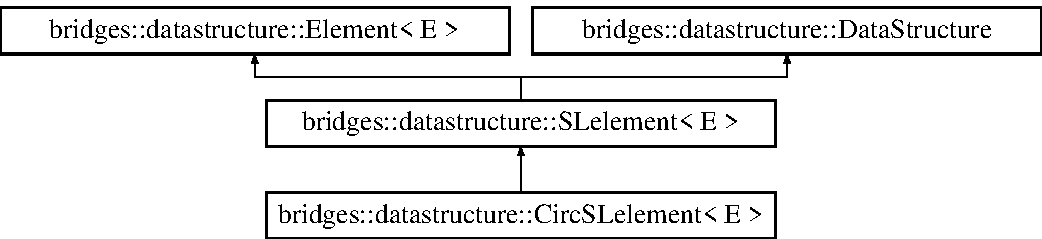
\includegraphics[height=3.000000cm]{classbridges_1_1datastructure_1_1_circ_s_lelement}
\end{center}
\end{figure}


\subsection{Detailed Description}
\subsubsection*{template$<$typename E$>$\newline
class bridges\+::datastructure\+::\+Circ\+S\+Lelement$<$ E $>$}

This class can be used to instantiate Singly Linked Circular List Elements. 

This class can be used to instantiate Circular (Singly) Linked List Elements, derived from Singly Linked \hyperlink{classbridges_1_1datastructure_1_1_element}{Element}. The main difference from the \hyperlink{classbridges_1_1datastructure_1_1_s_lelement}{S\+Lelement} is that they create circularly linked elements and their traversals are slightly different.

Elements have labels (string) that are displayed on the visualization Elements take an generic object as a user defined parameter, any native type or object.

\hyperlink{classbridges_1_1datastructure_1_1_element}{Element} contains a visualizer object for setting visual attributes (color, shape, opacity, size), necessary for displaying them in a web browser

\begin{DoxySeeAlso}{See also}
There is a tutorial about Circular Singly Linked Lists \+: \href{http://bridgesuncc.github.io/tutorials/CircularSinglyLinkedList.html}{\tt http\+://bridgesuncc.\+github.\+io/tutorials/\+Circular\+Singly\+Linked\+List.\+html}
\end{DoxySeeAlso}
\begin{DoxyAuthor}{Author}
Kalpathi Subramanian 
\end{DoxyAuthor}
\begin{DoxyDate}{Date}
10/5/2016, 7/12/19
\end{DoxyDate}

\begin{DoxyParams}{Parameters}
{\em E} & User type stored in the list \\
\hline
\end{DoxyParams}
\subsection*{Classes}
\begin{DoxyCompactItemize}
\item 
class \hyperlink{classbridges_1_1datastructure_1_1_circ_s_lelement_1_1_circ_s_lelement__constlisthelper}{Circ\+S\+Lelement\+\_\+constlisthelper}
\begin{DoxyCompactList}\small\item\em these are helper classes for \hyperlink{classbridges_1_1datastructure_1_1_circ_s_lelement}{Circ\+S\+Lelement} for easy iteration in a range for loop. It is not meant to be created by the bridges user. But it may be returned by \hyperlink{classbridges_1_1_bridges}{Bridges} to provide an S\+TL compliant list A\+PI. \end{DoxyCompactList}\item 
class \hyperlink{classbridges_1_1datastructure_1_1_circ_s_lelement_1_1_circ_s_lelement__listhelper}{Circ\+S\+Lelement\+\_\+listhelper}
\end{DoxyCompactItemize}
\subsection*{Public Member Functions}
\begin{DoxyCompactItemize}
\item 
\hyperlink{classbridges_1_1datastructure_1_1_circ_s_lelement_a3c79c117602d95cb150517b38442652e}{Circ\+S\+Lelement} ()
\item 
\hyperlink{classbridges_1_1datastructure_1_1_circ_s_lelement_a77f564922261b58522ddb244a8cea0dc}{Circ\+S\+Lelement} (E val=E(), string label=string())
\item 
\hyperlink{classbridges_1_1datastructure_1_1_circ_s_lelement_aaedaa1d980bd5a66511b57cd20a8d94c}{Circ\+S\+Lelement} (E e=E(), \hyperlink{classbridges_1_1datastructure_1_1_circ_s_lelement}{Circ\+S\+Lelement} $\ast$\hyperlink{classbridges_1_1datastructure_1_1_s_lelement_afc016a593a4a5aba82021ee34edadbfc}{next}=nullptr)
\item 
\hyperlink{classbridges_1_1datastructure_1_1_circ_s_lelement_a89f06ba76b1fdf1d2343c5f18f226722}{Circ\+S\+Lelement} (\hyperlink{classbridges_1_1datastructure_1_1_circ_s_lelement}{Circ\+S\+Lelement} $\ast$\hyperlink{classbridges_1_1datastructure_1_1_s_lelement_afc016a593a4a5aba82021ee34edadbfc}{next})
\item 
virtual const string \hyperlink{classbridges_1_1datastructure_1_1_circ_s_lelement_a775ba08a7811fe91c396cb27ba9343ab}{get\+D\+Stype} () const override
\item 
virtual \hyperlink{classbridges_1_1datastructure_1_1_circ_s_lelement}{Circ\+S\+Lelement}$<$ E $>$ $\ast$ \hyperlink{classbridges_1_1datastructure_1_1_circ_s_lelement_aff77056ace1361a35a09dc006eba34a3}{get\+Next} () override
\item 
void \hyperlink{classbridges_1_1datastructure_1_1_circ_s_lelement_a623d302217fce43a444e6da5e1de9b40}{set\+Next} (\hyperlink{classbridges_1_1datastructure_1_1_circ_s_lelement}{Circ\+S\+Lelement}$<$ E $>$ $\ast$\hyperlink{classbridges_1_1datastructure_1_1_s_lelement_afc016a593a4a5aba82021ee34edadbfc}{next})
\end{DoxyCompactItemize}
\subsection*{Additional Inherited Members}


\subsection{Constructor \& Destructor Documentation}
\mbox{\Hypertarget{classbridges_1_1datastructure_1_1_circ_s_lelement_a3c79c117602d95cb150517b38442652e}\label{classbridges_1_1datastructure_1_1_circ_s_lelement_a3c79c117602d95cb150517b38442652e}} 
\index{bridges\+::datastructure\+::\+Circ\+S\+Lelement@{bridges\+::datastructure\+::\+Circ\+S\+Lelement}!Circ\+S\+Lelement@{Circ\+S\+Lelement}}
\index{Circ\+S\+Lelement@{Circ\+S\+Lelement}!bridges\+::datastructure\+::\+Circ\+S\+Lelement@{bridges\+::datastructure\+::\+Circ\+S\+Lelement}}
\subsubsection{\texorpdfstring{Circ\+S\+Lelement()}{CircSLelement()}\hspace{0.1cm}{\footnotesize\ttfamily [1/4]}}
{\footnotesize\ttfamily template$<$typename E$>$ \\
\hyperlink{classbridges_1_1datastructure_1_1_circ_s_lelement}{bridges\+::datastructure\+::\+Circ\+S\+Lelement}$<$ E $>$\+::\hyperlink{classbridges_1_1datastructure_1_1_circ_s_lelement}{Circ\+S\+Lelement} (\begin{DoxyParamCaption}{ }\end{DoxyParamCaption})\hspace{0.3cm}{\ttfamily [inline]}}

This constructor creates an \hyperlink{classbridges_1_1datastructure_1_1_circ_s_lelement}{Circ\+S\+Lelement} object and sets its next pointer to itself \mbox{\Hypertarget{classbridges_1_1datastructure_1_1_circ_s_lelement_a77f564922261b58522ddb244a8cea0dc}\label{classbridges_1_1datastructure_1_1_circ_s_lelement_a77f564922261b58522ddb244a8cea0dc}} 
\index{bridges\+::datastructure\+::\+Circ\+S\+Lelement@{bridges\+::datastructure\+::\+Circ\+S\+Lelement}!Circ\+S\+Lelement@{Circ\+S\+Lelement}}
\index{Circ\+S\+Lelement@{Circ\+S\+Lelement}!bridges\+::datastructure\+::\+Circ\+S\+Lelement@{bridges\+::datastructure\+::\+Circ\+S\+Lelement}}
\subsubsection{\texorpdfstring{Circ\+S\+Lelement()}{CircSLelement()}\hspace{0.1cm}{\footnotesize\ttfamily [2/4]}}
{\footnotesize\ttfamily template$<$typename E$>$ \\
\hyperlink{classbridges_1_1datastructure_1_1_circ_s_lelement}{bridges\+::datastructure\+::\+Circ\+S\+Lelement}$<$ E $>$\+::\hyperlink{classbridges_1_1datastructure_1_1_circ_s_lelement}{Circ\+S\+Lelement} (\begin{DoxyParamCaption}\item[{E}]{val = {\ttfamily E()},  }\item[{string}]{label = {\ttfamily string()} }\end{DoxyParamCaption})\hspace{0.3cm}{\ttfamily [inline]}}

This constructor creates an \hyperlink{classbridges_1_1datastructure_1_1_circ_s_lelement}{Circ\+S\+Lelement} object of value \char`\"{}e\char`\"{} and label \char`\"{}label\char`\"{} and sets the next pointer to null


\begin{DoxyParams}{Parameters}
{\em label} & the label of \hyperlink{classbridges_1_1datastructure_1_1_circ_s_lelement}{Circ\+S\+Lelement} that shows up on the \hyperlink{classbridges_1_1_bridges}{Bridges} visualization \\
\hline
{\em val} & the generic object that this \hyperlink{classbridges_1_1datastructure_1_1_circ_s_lelement}{Circ\+S\+Lelement} will hold \\
\hline
\end{DoxyParams}
\mbox{\Hypertarget{classbridges_1_1datastructure_1_1_circ_s_lelement_aaedaa1d980bd5a66511b57cd20a8d94c}\label{classbridges_1_1datastructure_1_1_circ_s_lelement_aaedaa1d980bd5a66511b57cd20a8d94c}} 
\index{bridges\+::datastructure\+::\+Circ\+S\+Lelement@{bridges\+::datastructure\+::\+Circ\+S\+Lelement}!Circ\+S\+Lelement@{Circ\+S\+Lelement}}
\index{Circ\+S\+Lelement@{Circ\+S\+Lelement}!bridges\+::datastructure\+::\+Circ\+S\+Lelement@{bridges\+::datastructure\+::\+Circ\+S\+Lelement}}
\subsubsection{\texorpdfstring{Circ\+S\+Lelement()}{CircSLelement()}\hspace{0.1cm}{\footnotesize\ttfamily [3/4]}}
{\footnotesize\ttfamily template$<$typename E$>$ \\
\hyperlink{classbridges_1_1datastructure_1_1_circ_s_lelement}{bridges\+::datastructure\+::\+Circ\+S\+Lelement}$<$ E $>$\+::\hyperlink{classbridges_1_1datastructure_1_1_circ_s_lelement}{Circ\+S\+Lelement} (\begin{DoxyParamCaption}\item[{E}]{e = {\ttfamily E()},  }\item[{\hyperlink{classbridges_1_1datastructure_1_1_circ_s_lelement}{Circ\+S\+Lelement}$<$ E $>$ $\ast$}]{next = {\ttfamily nullptr} }\end{DoxyParamCaption})\hspace{0.3cm}{\ttfamily [inline]}}

Creates a new element with value \char`\"{}e\char`\"{} and sets the next pointer to the \hyperlink{classbridges_1_1datastructure_1_1_circ_s_lelement}{Circ\+S\+Lelement} referenced by the \char`\"{}next\char`\"{} argument


\begin{DoxyParams}{Parameters}
{\em e} & the generic object that this \hyperlink{classbridges_1_1datastructure_1_1_circ_s_lelement}{Circ\+S\+Lelement} will hold \\
\hline
{\em next} & the \hyperlink{classbridges_1_1datastructure_1_1_circ_s_lelement}{Circ\+S\+Lelement} that should be assigned to the next pointer \\
\hline
\end{DoxyParams}
\mbox{\Hypertarget{classbridges_1_1datastructure_1_1_circ_s_lelement_a89f06ba76b1fdf1d2343c5f18f226722}\label{classbridges_1_1datastructure_1_1_circ_s_lelement_a89f06ba76b1fdf1d2343c5f18f226722}} 
\index{bridges\+::datastructure\+::\+Circ\+S\+Lelement@{bridges\+::datastructure\+::\+Circ\+S\+Lelement}!Circ\+S\+Lelement@{Circ\+S\+Lelement}}
\index{Circ\+S\+Lelement@{Circ\+S\+Lelement}!bridges\+::datastructure\+::\+Circ\+S\+Lelement@{bridges\+::datastructure\+::\+Circ\+S\+Lelement}}
\subsubsection{\texorpdfstring{Circ\+S\+Lelement()}{CircSLelement()}\hspace{0.1cm}{\footnotesize\ttfamily [4/4]}}
{\footnotesize\ttfamily template$<$typename E$>$ \\
\hyperlink{classbridges_1_1datastructure_1_1_circ_s_lelement}{bridges\+::datastructure\+::\+Circ\+S\+Lelement}$<$ E $>$\+::\hyperlink{classbridges_1_1datastructure_1_1_circ_s_lelement}{Circ\+S\+Lelement} (\begin{DoxyParamCaption}\item[{\hyperlink{classbridges_1_1datastructure_1_1_circ_s_lelement}{Circ\+S\+Lelement}$<$ E $>$ $\ast$}]{next }\end{DoxyParamCaption})\hspace{0.3cm}{\ttfamily [inline]}}

Creates a new element and sets the next pointer to the \hyperlink{classbridges_1_1datastructure_1_1_circ_s_lelement}{Circ\+S\+Lelement} \char`\"{}next\char`\"{} 
\begin{DoxyParams}{Parameters}
{\em next} & the \hyperlink{classbridges_1_1datastructure_1_1_circ_s_lelement}{Circ\+S\+Lelement} that should be assigned to the next pointer \\
\hline
\end{DoxyParams}


\subsection{Member Function Documentation}
\mbox{\Hypertarget{classbridges_1_1datastructure_1_1_circ_s_lelement_a775ba08a7811fe91c396cb27ba9343ab}\label{classbridges_1_1datastructure_1_1_circ_s_lelement_a775ba08a7811fe91c396cb27ba9343ab}} 
\index{bridges\+::datastructure\+::\+Circ\+S\+Lelement@{bridges\+::datastructure\+::\+Circ\+S\+Lelement}!get\+D\+Stype@{get\+D\+Stype}}
\index{get\+D\+Stype@{get\+D\+Stype}!bridges\+::datastructure\+::\+Circ\+S\+Lelement@{bridges\+::datastructure\+::\+Circ\+S\+Lelement}}
\subsubsection{\texorpdfstring{get\+D\+Stype()}{getDStype()}}
{\footnotesize\ttfamily template$<$typename E$>$ \\
virtual const string \hyperlink{classbridges_1_1datastructure_1_1_circ_s_lelement}{bridges\+::datastructure\+::\+Circ\+S\+Lelement}$<$ E $>$\+::get\+D\+Stype (\begin{DoxyParamCaption}{ }\end{DoxyParamCaption}) const\hspace{0.3cm}{\ttfamily [inline]}, {\ttfamily [override]}, {\ttfamily [virtual]}}

This method gets the data structure type

\begin{DoxyReturn}{Returns}
The date structure name 
\end{DoxyReturn}


Reimplemented from \hyperlink{classbridges_1_1datastructure_1_1_s_lelement_a602156aacacd73d1faa365d68d8af31b}{bridges\+::datastructure\+::\+S\+Lelement$<$ E $>$}.

\mbox{\Hypertarget{classbridges_1_1datastructure_1_1_circ_s_lelement_aff77056ace1361a35a09dc006eba34a3}\label{classbridges_1_1datastructure_1_1_circ_s_lelement_aff77056ace1361a35a09dc006eba34a3}} 
\index{bridges\+::datastructure\+::\+Circ\+S\+Lelement@{bridges\+::datastructure\+::\+Circ\+S\+Lelement}!get\+Next@{get\+Next}}
\index{get\+Next@{get\+Next}!bridges\+::datastructure\+::\+Circ\+S\+Lelement@{bridges\+::datastructure\+::\+Circ\+S\+Lelement}}
\subsubsection{\texorpdfstring{get\+Next()}{getNext()}}
{\footnotesize\ttfamily template$<$typename E$>$ \\
virtual \hyperlink{classbridges_1_1datastructure_1_1_circ_s_lelement}{Circ\+S\+Lelement}$<$E$>$$\ast$ \hyperlink{classbridges_1_1datastructure_1_1_circ_s_lelement}{bridges\+::datastructure\+::\+Circ\+S\+Lelement}$<$ E $>$\+::get\+Next (\begin{DoxyParamCaption}{ }\end{DoxyParamCaption})\hspace{0.3cm}{\ttfamily [inline]}, {\ttfamily [override]}, {\ttfamily [virtual]}}

Retrieves the next \hyperlink{classbridges_1_1datastructure_1_1_circ_s_lelement}{Circ\+S\+Lelement} \begin{DoxyReturn}{Returns}
the next element in the list 
\end{DoxyReturn}


Reimplemented from \hyperlink{classbridges_1_1datastructure_1_1_s_lelement_ae43dd771d9ced7cb17f1d35f34cd9a42}{bridges\+::datastructure\+::\+S\+Lelement$<$ E $>$}.

\mbox{\Hypertarget{classbridges_1_1datastructure_1_1_circ_s_lelement_a623d302217fce43a444e6da5e1de9b40}\label{classbridges_1_1datastructure_1_1_circ_s_lelement_a623d302217fce43a444e6da5e1de9b40}} 
\index{bridges\+::datastructure\+::\+Circ\+S\+Lelement@{bridges\+::datastructure\+::\+Circ\+S\+Lelement}!set\+Next@{set\+Next}}
\index{set\+Next@{set\+Next}!bridges\+::datastructure\+::\+Circ\+S\+Lelement@{bridges\+::datastructure\+::\+Circ\+S\+Lelement}}
\subsubsection{\texorpdfstring{set\+Next()}{setNext()}}
{\footnotesize\ttfamily template$<$typename E$>$ \\
void \hyperlink{classbridges_1_1datastructure_1_1_circ_s_lelement}{bridges\+::datastructure\+::\+Circ\+S\+Lelement}$<$ E $>$\+::set\+Next (\begin{DoxyParamCaption}\item[{\hyperlink{classbridges_1_1datastructure_1_1_circ_s_lelement}{Circ\+S\+Lelement}$<$ E $>$ $\ast$}]{next }\end{DoxyParamCaption})\hspace{0.3cm}{\ttfamily [inline]}}

Sets the pointer to the next \hyperlink{classbridges_1_1datastructure_1_1_circ_s_lelement}{Circ\+S\+Lelement} 
\begin{DoxyParams}{Parameters}
{\em next} & Circ\+S\+Lelement$<$\+E$>$ that should be assigned to the next pointer \\
\hline
\end{DoxyParams}


The documentation for this class was generated from the following file\+:\begin{DoxyCompactItemize}
\item 
/home/erik/work/bridges/bridges-\/cxx/src/\hyperlink{_circ_s_lelement_8h}{Circ\+S\+Lelement.\+h}\end{DoxyCompactItemize}

\hypertarget{classbridges_1_1datastructure_1_1_circ_s_lelement_1_1_circ_s_lelement__constlisthelper}{}\doxysection{bridges\+::datastructure\+::Circ\+SLelement$<$ E $>$\+::Circ\+SLelement\+\_\+constlisthelper Class Reference}
\label{classbridges_1_1datastructure_1_1_circ_s_lelement_1_1_circ_s_lelement__constlisthelper}\index{bridges::datastructure::CircSLelement$<$ E $>$::CircSLelement\_constlisthelper@{bridges::datastructure::CircSLelement$<$ E $>$::CircSLelement\_constlisthelper}}


{\ttfamily \#include $<$Circ\+SLelement.\+h$>$}



\doxysubsection{Detailed Description}
\subsubsection*{template$<$typename E$>$\newline
class bridges\+::datastructure\+::\+Circ\+SLelement$<$ E $>$\+::\+Circ\+SLelement\+\_\+constlisthelper}

these are helper classes for \mbox{\hyperlink{classbridges_1_1datastructure_1_1_circ_s_lelement}{Circ\+SLelement}} for easy iteration in a range for loop. It is not meant to be created by the bridges user. But it may be returned by \mbox{\hyperlink{classbridges_1_1_bridges}{Bridges}} to provide an STL compliant list API. \doxysubsection*{Classes}
\begin{DoxyCompactItemize}
\item 
class \mbox{\hyperlink{classbridges_1_1datastructure_1_1_circ_s_lelement_1_1_circ_s_lelement__constlisthelper_1_1iterator}{iterator}}
\end{DoxyCompactItemize}
\doxysubsection*{Public Member Functions}
\begin{DoxyCompactItemize}
\item 
\mbox{\hyperlink{classbridges_1_1datastructure_1_1_circ_s_lelement_1_1_circ_s_lelement__constlisthelper_af174ab008506dd4b814660e6abc571b1}{Circ\+SLelement\+\_\+constlisthelper}} (typename \mbox{\hyperlink{classbridges_1_1datastructure_1_1_circ_s_lelement}{bridges\+::datastructure\+::\+Circ\+SLelement}}$<$ E $>$ const $\ast$s)
\item 
\mbox{\hyperlink{classbridges_1_1datastructure_1_1_circ_s_lelement_1_1_circ_s_lelement__constlisthelper_1_1iterator}{iterator}} \mbox{\hyperlink{classbridges_1_1datastructure_1_1_circ_s_lelement_1_1_circ_s_lelement__constlisthelper_a57653761fb7c0ad519a9415c77d1f4c4}{begin}} ()
\item 
\mbox{\hyperlink{classbridges_1_1datastructure_1_1_circ_s_lelement_1_1_circ_s_lelement__constlisthelper_1_1iterator}{iterator}} \mbox{\hyperlink{classbridges_1_1datastructure_1_1_circ_s_lelement_1_1_circ_s_lelement__constlisthelper_a93f42a63638e54e427648d7182b44d42}{end}} ()
\end{DoxyCompactItemize}


\doxysubsection{Constructor \& Destructor Documentation}
\mbox{\Hypertarget{classbridges_1_1datastructure_1_1_circ_s_lelement_1_1_circ_s_lelement__constlisthelper_af174ab008506dd4b814660e6abc571b1}\label{classbridges_1_1datastructure_1_1_circ_s_lelement_1_1_circ_s_lelement__constlisthelper_af174ab008506dd4b814660e6abc571b1}} 
\index{bridges::datastructure::CircSLelement$<$ E $>$::CircSLelement\_constlisthelper@{bridges::datastructure::CircSLelement$<$ E $>$::CircSLelement\_constlisthelper}!CircSLelement\_constlisthelper@{CircSLelement\_constlisthelper}}
\index{CircSLelement\_constlisthelper@{CircSLelement\_constlisthelper}!bridges::datastructure::CircSLelement$<$ E $>$::CircSLelement\_constlisthelper@{bridges::datastructure::CircSLelement$<$ E $>$::CircSLelement\_constlisthelper}}
\doxysubsubsection{\texorpdfstring{CircSLelement\_constlisthelper()}{CircSLelement\_constlisthelper()}}
{\footnotesize\ttfamily template$<$typename E $>$ \\
\mbox{\hyperlink{classbridges_1_1datastructure_1_1_circ_s_lelement}{bridges\+::datastructure\+::\+Circ\+SLelement}}$<$ E $>$\+::Circ\+SLelement\+\_\+constlisthelper\+::\+Circ\+SLelement\+\_\+constlisthelper (\begin{DoxyParamCaption}\item[{typename \mbox{\hyperlink{classbridges_1_1datastructure_1_1_circ_s_lelement}{bridges\+::datastructure\+::\+Circ\+SLelement}}$<$ E $>$ const $\ast$}]{s }\end{DoxyParamCaption})\hspace{0.3cm}{\ttfamily [inline]}}



\doxysubsection{Member Function Documentation}
\mbox{\Hypertarget{classbridges_1_1datastructure_1_1_circ_s_lelement_1_1_circ_s_lelement__constlisthelper_a57653761fb7c0ad519a9415c77d1f4c4}\label{classbridges_1_1datastructure_1_1_circ_s_lelement_1_1_circ_s_lelement__constlisthelper_a57653761fb7c0ad519a9415c77d1f4c4}} 
\index{bridges::datastructure::CircSLelement$<$ E $>$::CircSLelement\_constlisthelper@{bridges::datastructure::CircSLelement$<$ E $>$::CircSLelement\_constlisthelper}!begin@{begin}}
\index{begin@{begin}!bridges::datastructure::CircSLelement$<$ E $>$::CircSLelement\_constlisthelper@{bridges::datastructure::CircSLelement$<$ E $>$::CircSLelement\_constlisthelper}}
\doxysubsubsection{\texorpdfstring{begin()}{begin()}}
{\footnotesize\ttfamily template$<$typename E $>$ \\
\mbox{\hyperlink{classbridges_1_1datastructure_1_1_circ_s_lelement_1_1_circ_s_lelement__constlisthelper_1_1iterator}{iterator}} \mbox{\hyperlink{classbridges_1_1datastructure_1_1_circ_s_lelement}{bridges\+::datastructure\+::\+Circ\+SLelement}}$<$ E $>$\+::Circ\+SLelement\+\_\+constlisthelper\+::begin (\begin{DoxyParamCaption}{ }\end{DoxyParamCaption})\hspace{0.3cm}{\ttfamily [inline]}}

\mbox{\Hypertarget{classbridges_1_1datastructure_1_1_circ_s_lelement_1_1_circ_s_lelement__constlisthelper_a93f42a63638e54e427648d7182b44d42}\label{classbridges_1_1datastructure_1_1_circ_s_lelement_1_1_circ_s_lelement__constlisthelper_a93f42a63638e54e427648d7182b44d42}} 
\index{bridges::datastructure::CircSLelement$<$ E $>$::CircSLelement\_constlisthelper@{bridges::datastructure::CircSLelement$<$ E $>$::CircSLelement\_constlisthelper}!end@{end}}
\index{end@{end}!bridges::datastructure::CircSLelement$<$ E $>$::CircSLelement\_constlisthelper@{bridges::datastructure::CircSLelement$<$ E $>$::CircSLelement\_constlisthelper}}
\doxysubsubsection{\texorpdfstring{end()}{end()}}
{\footnotesize\ttfamily template$<$typename E $>$ \\
\mbox{\hyperlink{classbridges_1_1datastructure_1_1_circ_s_lelement_1_1_circ_s_lelement__constlisthelper_1_1iterator}{iterator}} \mbox{\hyperlink{classbridges_1_1datastructure_1_1_circ_s_lelement}{bridges\+::datastructure\+::\+Circ\+SLelement}}$<$ E $>$\+::Circ\+SLelement\+\_\+constlisthelper\+::end (\begin{DoxyParamCaption}{ }\end{DoxyParamCaption})\hspace{0.3cm}{\ttfamily [inline]}}



The documentation for this class was generated from the following file\+:\begin{DoxyCompactItemize}
\item 
/home/erik/work/bridges/bridges-\/cxx/src/\mbox{\hyperlink{_circ_s_lelement_8h}{Circ\+SLelement.\+h}}\end{DoxyCompactItemize}

\hypertarget{classbridges_1_1datastructure_1_1_circ_s_lelement_1_1_circ_s_lelement__listhelper}{}\section{bridges\+:\+:datastructure\+:\+:Circ\+S\+Lelement$<$ E $>$\+:\+:Circ\+S\+Lelement\+\_\+listhelper Class Reference}
\label{classbridges_1_1datastructure_1_1_circ_s_lelement_1_1_circ_s_lelement__listhelper}\index{bridges\+::datastructure\+::\+Circ\+S\+Lelement$<$ E $>$\+::\+Circ\+S\+Lelement\+\_\+listhelper@{bridges\+::datastructure\+::\+Circ\+S\+Lelement$<$ E $>$\+::\+Circ\+S\+Lelement\+\_\+listhelper}}


{\ttfamily \#include $<$Circ\+S\+Lelement.\+h$>$}

\subsection*{Classes}
\begin{DoxyCompactItemize}
\item 
class \hyperlink{classbridges_1_1datastructure_1_1_circ_s_lelement_1_1_circ_s_lelement__listhelper_1_1iterator}{iterator}
\end{DoxyCompactItemize}
\subsection*{Public Member Functions}
\begin{DoxyCompactItemize}
\item 
\hyperlink{classbridges_1_1datastructure_1_1_circ_s_lelement_1_1_circ_s_lelement__listhelper_acbdfc2d3415b54a52bb3b5e7b4bc9929}{Circ\+S\+Lelement\+\_\+listhelper} (typename \hyperlink{classbridges_1_1datastructure_1_1_circ_s_lelement}{bridges\+::datastructure\+::\+Circ\+S\+Lelement}$<$ E $>$ $\ast$s)
\item 
\hyperlink{classbridges_1_1datastructure_1_1_circ_s_lelement_1_1_circ_s_lelement__listhelper_1_1iterator}{iterator} \hyperlink{classbridges_1_1datastructure_1_1_circ_s_lelement_1_1_circ_s_lelement__listhelper_aa1294a519be56c74beec21d2c4a13864}{begin} ()
\item 
\hyperlink{classbridges_1_1datastructure_1_1_circ_s_lelement_1_1_circ_s_lelement__listhelper_1_1iterator}{iterator} \hyperlink{classbridges_1_1datastructure_1_1_circ_s_lelement_1_1_circ_s_lelement__listhelper_aceac5cae38d478dd16d2e44f329ea821}{end} ()
\end{DoxyCompactItemize}


\subsection{Constructor \& Destructor Documentation}
\mbox{\Hypertarget{classbridges_1_1datastructure_1_1_circ_s_lelement_1_1_circ_s_lelement__listhelper_acbdfc2d3415b54a52bb3b5e7b4bc9929}\label{classbridges_1_1datastructure_1_1_circ_s_lelement_1_1_circ_s_lelement__listhelper_acbdfc2d3415b54a52bb3b5e7b4bc9929}} 
\index{bridges\+::datastructure\+::\+Circ\+S\+Lelement\+::\+Circ\+S\+Lelement\+\_\+listhelper@{bridges\+::datastructure\+::\+Circ\+S\+Lelement\+::\+Circ\+S\+Lelement\+\_\+listhelper}!Circ\+S\+Lelement\+\_\+listhelper@{Circ\+S\+Lelement\+\_\+listhelper}}
\index{Circ\+S\+Lelement\+\_\+listhelper@{Circ\+S\+Lelement\+\_\+listhelper}!bridges\+::datastructure\+::\+Circ\+S\+Lelement\+::\+Circ\+S\+Lelement\+\_\+listhelper@{bridges\+::datastructure\+::\+Circ\+S\+Lelement\+::\+Circ\+S\+Lelement\+\_\+listhelper}}
\subsubsection{\texorpdfstring{Circ\+S\+Lelement\+\_\+listhelper()}{CircSLelement\_listhelper()}}
{\footnotesize\ttfamily template$<$typename E$>$ \\
\hyperlink{classbridges_1_1datastructure_1_1_circ_s_lelement}{bridges\+::datastructure\+::\+Circ\+S\+Lelement}$<$ E $>$\+::Circ\+S\+Lelement\+\_\+listhelper\+::\+Circ\+S\+Lelement\+\_\+listhelper (\begin{DoxyParamCaption}\item[{typename \hyperlink{classbridges_1_1datastructure_1_1_circ_s_lelement}{bridges\+::datastructure\+::\+Circ\+S\+Lelement}$<$ E $>$ $\ast$}]{s }\end{DoxyParamCaption})\hspace{0.3cm}{\ttfamily [inline]}}



\subsection{Member Function Documentation}
\mbox{\Hypertarget{classbridges_1_1datastructure_1_1_circ_s_lelement_1_1_circ_s_lelement__listhelper_aa1294a519be56c74beec21d2c4a13864}\label{classbridges_1_1datastructure_1_1_circ_s_lelement_1_1_circ_s_lelement__listhelper_aa1294a519be56c74beec21d2c4a13864}} 
\index{bridges\+::datastructure\+::\+Circ\+S\+Lelement\+::\+Circ\+S\+Lelement\+\_\+listhelper@{bridges\+::datastructure\+::\+Circ\+S\+Lelement\+::\+Circ\+S\+Lelement\+\_\+listhelper}!begin@{begin}}
\index{begin@{begin}!bridges\+::datastructure\+::\+Circ\+S\+Lelement\+::\+Circ\+S\+Lelement\+\_\+listhelper@{bridges\+::datastructure\+::\+Circ\+S\+Lelement\+::\+Circ\+S\+Lelement\+\_\+listhelper}}
\subsubsection{\texorpdfstring{begin()}{begin()}}
{\footnotesize\ttfamily template$<$typename E$>$ \\
\hyperlink{classbridges_1_1datastructure_1_1_circ_s_lelement_1_1_circ_s_lelement__listhelper_1_1iterator}{iterator} \hyperlink{classbridges_1_1datastructure_1_1_circ_s_lelement}{bridges\+::datastructure\+::\+Circ\+S\+Lelement}$<$ E $>$\+::Circ\+S\+Lelement\+\_\+listhelper\+::begin (\begin{DoxyParamCaption}{ }\end{DoxyParamCaption})\hspace{0.3cm}{\ttfamily [inline]}}

\mbox{\Hypertarget{classbridges_1_1datastructure_1_1_circ_s_lelement_1_1_circ_s_lelement__listhelper_aceac5cae38d478dd16d2e44f329ea821}\label{classbridges_1_1datastructure_1_1_circ_s_lelement_1_1_circ_s_lelement__listhelper_aceac5cae38d478dd16d2e44f329ea821}} 
\index{bridges\+::datastructure\+::\+Circ\+S\+Lelement\+::\+Circ\+S\+Lelement\+\_\+listhelper@{bridges\+::datastructure\+::\+Circ\+S\+Lelement\+::\+Circ\+S\+Lelement\+\_\+listhelper}!end@{end}}
\index{end@{end}!bridges\+::datastructure\+::\+Circ\+S\+Lelement\+::\+Circ\+S\+Lelement\+\_\+listhelper@{bridges\+::datastructure\+::\+Circ\+S\+Lelement\+::\+Circ\+S\+Lelement\+\_\+listhelper}}
\subsubsection{\texorpdfstring{end()}{end()}}
{\footnotesize\ttfamily template$<$typename E$>$ \\
\hyperlink{classbridges_1_1datastructure_1_1_circ_s_lelement_1_1_circ_s_lelement__listhelper_1_1iterator}{iterator} \hyperlink{classbridges_1_1datastructure_1_1_circ_s_lelement}{bridges\+::datastructure\+::\+Circ\+S\+Lelement}$<$ E $>$\+::Circ\+S\+Lelement\+\_\+listhelper\+::end (\begin{DoxyParamCaption}{ }\end{DoxyParamCaption})\hspace{0.3cm}{\ttfamily [inline]}}



The documentation for this class was generated from the following file\+:\begin{DoxyCompactItemize}
\item 
/home/erik/work/bridges/bridges-\/cxx/src/\hyperlink{_circ_s_lelement_8h}{Circ\+S\+Lelement.\+h}\end{DoxyCompactItemize}

\hypertarget{classsio_1_1client}{}\doxysection{sio\+::client Class Reference}
\label{classsio_1_1client}\index{sio::client@{sio::client}}


{\ttfamily \#include $<$sio\+\_\+client.\+h$>$}

\doxysubsection*{Public Types}
\begin{DoxyCompactItemize}
\item 
enum \mbox{\hyperlink{classsio_1_1client_a5c8b6c424134f40b3e9bf488b4961aaf}{close\+\_\+reason}} \{ \mbox{\hyperlink{classsio_1_1client_a5c8b6c424134f40b3e9bf488b4961aafa3d0f427321567c717587a633793c5198}{close\+\_\+reason\+\_\+normal}}
, \mbox{\hyperlink{classsio_1_1client_a5c8b6c424134f40b3e9bf488b4961aafa2066afdaa7a1383099c527b5c1aaa777}{close\+\_\+reason\+\_\+drop}}
 \}
\item 
typedef std\+::function$<$ void(void)$>$ \mbox{\hyperlink{classsio_1_1client_a23951b626c91c87e866d4e966ec828fa}{con\+\_\+listener}}
\item 
typedef std\+::function$<$ void(\mbox{\hyperlink{classsio_1_1client_a5c8b6c424134f40b3e9bf488b4961aaf}{close\+\_\+reason}} const  \&reason)$>$ \mbox{\hyperlink{classsio_1_1client_a9736334c566e7dcc6201ea5629024390}{close\+\_\+listener}}
\item 
typedef std\+::function$<$ void(unsigned, unsigned)$>$ \mbox{\hyperlink{classsio_1_1client_a62a35170a39347cb1e56e2105badcad1}{reconnect\+\_\+listener}}
\item 
typedef std\+::function$<$ void(std\+::string const  \&nsp)$>$ \mbox{\hyperlink{classsio_1_1client_a02b43cadd1588575ae2465042452cabf}{socket\+\_\+listener}}
\end{DoxyCompactItemize}
\doxysubsection*{Public Member Functions}
\begin{DoxyCompactItemize}
\item 
\mbox{\hyperlink{classsio_1_1client_a409f7973576dd3ce5ae8d717d0962bcc}{client}} ()
\item 
\mbox{\hyperlink{classsio_1_1client_ac9ec4634825ee92ffdc37b145d04872e}{$\sim$client}} ()
\item 
void \mbox{\hyperlink{classsio_1_1client_a4cd8f0f1e1cc6cf0ee0e43c4b60cd2d6}{set\+\_\+open\+\_\+listener}} (\mbox{\hyperlink{classsio_1_1client_a23951b626c91c87e866d4e966ec828fa}{con\+\_\+listener}} const \&l)
\item 
void \mbox{\hyperlink{classsio_1_1client_aa771d523e50a3b431ed894133fec12aa}{set\+\_\+fail\+\_\+listener}} (\mbox{\hyperlink{classsio_1_1client_a23951b626c91c87e866d4e966ec828fa}{con\+\_\+listener}} const \&l)
\item 
void \mbox{\hyperlink{classsio_1_1client_a5d8ba15169b4fdb346c36359f2716d78}{set\+\_\+reconnecting\+\_\+listener}} (\mbox{\hyperlink{classsio_1_1client_a23951b626c91c87e866d4e966ec828fa}{con\+\_\+listener}} const \&l)
\item 
void \mbox{\hyperlink{classsio_1_1client_a321e1bcf29625eea691dab0cd1d78ee9}{set\+\_\+reconnect\+\_\+listener}} (\mbox{\hyperlink{classsio_1_1client_a62a35170a39347cb1e56e2105badcad1}{reconnect\+\_\+listener}} const \&l)
\item 
void \mbox{\hyperlink{classsio_1_1client_a85a00dc13d6c43d5fd710805e63569b1}{set\+\_\+close\+\_\+listener}} (\mbox{\hyperlink{classsio_1_1client_a9736334c566e7dcc6201ea5629024390}{close\+\_\+listener}} const \&l)
\item 
void \mbox{\hyperlink{classsio_1_1client_a49821e44c763e2b96def29bf4d2d00ad}{set\+\_\+socket\+\_\+open\+\_\+listener}} (\mbox{\hyperlink{classsio_1_1client_a02b43cadd1588575ae2465042452cabf}{socket\+\_\+listener}} const \&l)
\item 
void \mbox{\hyperlink{classsio_1_1client_ac95e53ccbde50dee8f314a26caf41bd3}{set\+\_\+socket\+\_\+close\+\_\+listener}} (\mbox{\hyperlink{classsio_1_1client_a02b43cadd1588575ae2465042452cabf}{socket\+\_\+listener}} const \&l)
\item 
void \mbox{\hyperlink{classsio_1_1client_a15eab3d354fef37eb2f7e671df494512}{clear\+\_\+con\+\_\+listeners}} ()
\item 
void \mbox{\hyperlink{classsio_1_1client_a07c0262b4ad4134fd5cc840a09fff93a}{clear\+\_\+socket\+\_\+listeners}} ()
\item 
void \mbox{\hyperlink{classsio_1_1client_a0e2cf12e2ededbc00ae1de22768c22ac}{connect}} (const std\+::string \&uri)
\item 
void \mbox{\hyperlink{classsio_1_1client_a3867f1379415ed97bd47a3d53458c273}{connect}} (const std\+::string \&uri, const std\+::map$<$ std\+::string, std\+::string $>$ \&query)
\item 
void \mbox{\hyperlink{classsio_1_1client_a9390bffe820269a81493f606e949b2b9}{connect}} (const std\+::string \&uri, const std\+::map$<$ std\+::string, std\+::string $>$ \&query, const std\+::map$<$ std\+::string, std\+::string $>$ \&http\+\_\+extra\+\_\+headers)
\item 
void \mbox{\hyperlink{classsio_1_1client_a42ae73ea487b59582742d914d3d93e05}{set\+\_\+reconnect\+\_\+attempts}} (int attempts)
\item 
void \mbox{\hyperlink{classsio_1_1client_a50da06327e202468a47e24c8b71d6864}{set\+\_\+reconnect\+\_\+delay}} (unsigned millis)
\item 
void \mbox{\hyperlink{classsio_1_1client_ab1339410ffe0ac1f7bf61236dafc5648}{set\+\_\+reconnect\+\_\+delay\+\_\+max}} (unsigned millis)
\item 
\mbox{\hyperlink{classsio_1_1socket_afb4f5829acfc5c8181ddb7174c501593}{sio\+::socket\+::ptr}} const  \& \mbox{\hyperlink{classsio_1_1client_a53459c95c2cd1c99ee7e6eec3181b947}{socket}} (const std\+::string \&nsp=\char`\"{}\char`\"{})
\item 
void \mbox{\hyperlink{classsio_1_1client_a1c36b90b0425246f74564e90f5263066}{close}} ()
\item 
void \mbox{\hyperlink{classsio_1_1client_a68787f325fdf4378b992329b123cde9d}{sync\+\_\+close}} ()
\item 
bool \mbox{\hyperlink{classsio_1_1client_afc1eb2298634f626d24e5fb0909ecb60}{opened}} () const
\item 
std\+::string const  \& \mbox{\hyperlink{classsio_1_1client_a3ff97f72d86f9fcad11bde729ac9d1b4}{get\+\_\+sessionid}} () const
\end{DoxyCompactItemize}


\doxysubsection{Member Typedef Documentation}
\mbox{\Hypertarget{classsio_1_1client_a9736334c566e7dcc6201ea5629024390}\label{classsio_1_1client_a9736334c566e7dcc6201ea5629024390}} 
\index{sio::client@{sio::client}!close\_listener@{close\_listener}}
\index{close\_listener@{close\_listener}!sio::client@{sio::client}}
\doxysubsubsection{\texorpdfstring{close\_listener}{close\_listener}}
{\footnotesize\ttfamily typedef std\+::function$<$void(\mbox{\hyperlink{classsio_1_1client_a5c8b6c424134f40b3e9bf488b4961aaf}{close\+\_\+reason}} const\& reason)$>$ \mbox{\hyperlink{classsio_1_1client_a9736334c566e7dcc6201ea5629024390}{sio\+::client\+::close\+\_\+listener}}}

\mbox{\Hypertarget{classsio_1_1client_a23951b626c91c87e866d4e966ec828fa}\label{classsio_1_1client_a23951b626c91c87e866d4e966ec828fa}} 
\index{sio::client@{sio::client}!con\_listener@{con\_listener}}
\index{con\_listener@{con\_listener}!sio::client@{sio::client}}
\doxysubsubsection{\texorpdfstring{con\_listener}{con\_listener}}
{\footnotesize\ttfamily typedef std\+::function$<$void(void)$>$ \mbox{\hyperlink{classsio_1_1client_a23951b626c91c87e866d4e966ec828fa}{sio\+::client\+::con\+\_\+listener}}}

\mbox{\Hypertarget{classsio_1_1client_a62a35170a39347cb1e56e2105badcad1}\label{classsio_1_1client_a62a35170a39347cb1e56e2105badcad1}} 
\index{sio::client@{sio::client}!reconnect\_listener@{reconnect\_listener}}
\index{reconnect\_listener@{reconnect\_listener}!sio::client@{sio::client}}
\doxysubsubsection{\texorpdfstring{reconnect\_listener}{reconnect\_listener}}
{\footnotesize\ttfamily typedef std\+::function$<$void(unsigned, unsigned)$>$ \mbox{\hyperlink{classsio_1_1client_a62a35170a39347cb1e56e2105badcad1}{sio\+::client\+::reconnect\+\_\+listener}}}

\mbox{\Hypertarget{classsio_1_1client_a02b43cadd1588575ae2465042452cabf}\label{classsio_1_1client_a02b43cadd1588575ae2465042452cabf}} 
\index{sio::client@{sio::client}!socket\_listener@{socket\_listener}}
\index{socket\_listener@{socket\_listener}!sio::client@{sio::client}}
\doxysubsubsection{\texorpdfstring{socket\_listener}{socket\_listener}}
{\footnotesize\ttfamily typedef std\+::function$<$void(std\+::string const\& nsp)$>$ \mbox{\hyperlink{classsio_1_1client_a02b43cadd1588575ae2465042452cabf}{sio\+::client\+::socket\+\_\+listener}}}



\doxysubsection{Member Enumeration Documentation}
\mbox{\Hypertarget{classsio_1_1client_a5c8b6c424134f40b3e9bf488b4961aaf}\label{classsio_1_1client_a5c8b6c424134f40b3e9bf488b4961aaf}} 
\index{sio::client@{sio::client}!close\_reason@{close\_reason}}
\index{close\_reason@{close\_reason}!sio::client@{sio::client}}
\doxysubsubsection{\texorpdfstring{close\_reason}{close\_reason}}
{\footnotesize\ttfamily enum \mbox{\hyperlink{classsio_1_1client_a5c8b6c424134f40b3e9bf488b4961aaf}{sio\+::client\+::close\+\_\+reason}}}

\begin{DoxyEnumFields}{Enumerator}
\raisebox{\heightof{T}}[0pt][0pt]{\index{close\_reason\_normal@{close\_reason\_normal}!sio::client@{sio::client}}\index{sio::client@{sio::client}!close\_reason\_normal@{close\_reason\_normal}}}\mbox{\Hypertarget{classsio_1_1client_a5c8b6c424134f40b3e9bf488b4961aafa3d0f427321567c717587a633793c5198}\label{classsio_1_1client_a5c8b6c424134f40b3e9bf488b4961aafa3d0f427321567c717587a633793c5198}} 
close\+\_\+reason\+\_\+normal&\\
\hline

\raisebox{\heightof{T}}[0pt][0pt]{\index{close\_reason\_drop@{close\_reason\_drop}!sio::client@{sio::client}}\index{sio::client@{sio::client}!close\_reason\_drop@{close\_reason\_drop}}}\mbox{\Hypertarget{classsio_1_1client_a5c8b6c424134f40b3e9bf488b4961aafa2066afdaa7a1383099c527b5c1aaa777}\label{classsio_1_1client_a5c8b6c424134f40b3e9bf488b4961aafa2066afdaa7a1383099c527b5c1aaa777}} 
close\+\_\+reason\+\_\+drop&\\
\hline

\end{DoxyEnumFields}


\doxysubsection{Constructor \& Destructor Documentation}
\mbox{\Hypertarget{classsio_1_1client_a409f7973576dd3ce5ae8d717d0962bcc}\label{classsio_1_1client_a409f7973576dd3ce5ae8d717d0962bcc}} 
\index{sio::client@{sio::client}!client@{client}}
\index{client@{client}!sio::client@{sio::client}}
\doxysubsubsection{\texorpdfstring{client()}{client()}}
{\footnotesize\ttfamily sio\+::client\+::client (\begin{DoxyParamCaption}{ }\end{DoxyParamCaption})}

\mbox{\Hypertarget{classsio_1_1client_ac9ec4634825ee92ffdc37b145d04872e}\label{classsio_1_1client_ac9ec4634825ee92ffdc37b145d04872e}} 
\index{sio::client@{sio::client}!````~client@{$\sim$client}}
\index{````~client@{$\sim$client}!sio::client@{sio::client}}
\doxysubsubsection{\texorpdfstring{$\sim$client()}{~client()}}
{\footnotesize\ttfamily sio\+::client\+::$\sim$client (\begin{DoxyParamCaption}{ }\end{DoxyParamCaption})}



\doxysubsection{Member Function Documentation}
\mbox{\Hypertarget{classsio_1_1client_a15eab3d354fef37eb2f7e671df494512}\label{classsio_1_1client_a15eab3d354fef37eb2f7e671df494512}} 
\index{sio::client@{sio::client}!clear\_con\_listeners@{clear\_con\_listeners}}
\index{clear\_con\_listeners@{clear\_con\_listeners}!sio::client@{sio::client}}
\doxysubsubsection{\texorpdfstring{clear\_con\_listeners()}{clear\_con\_listeners()}}
{\footnotesize\ttfamily void sio\+::client\+::clear\+\_\+con\+\_\+listeners (\begin{DoxyParamCaption}{ }\end{DoxyParamCaption})}

\mbox{\Hypertarget{classsio_1_1client_a07c0262b4ad4134fd5cc840a09fff93a}\label{classsio_1_1client_a07c0262b4ad4134fd5cc840a09fff93a}} 
\index{sio::client@{sio::client}!clear\_socket\_listeners@{clear\_socket\_listeners}}
\index{clear\_socket\_listeners@{clear\_socket\_listeners}!sio::client@{sio::client}}
\doxysubsubsection{\texorpdfstring{clear\_socket\_listeners()}{clear\_socket\_listeners()}}
{\footnotesize\ttfamily void sio\+::client\+::clear\+\_\+socket\+\_\+listeners (\begin{DoxyParamCaption}{ }\end{DoxyParamCaption})}

\mbox{\Hypertarget{classsio_1_1client_a1c36b90b0425246f74564e90f5263066}\label{classsio_1_1client_a1c36b90b0425246f74564e90f5263066}} 
\index{sio::client@{sio::client}!close@{close}}
\index{close@{close}!sio::client@{sio::client}}
\doxysubsubsection{\texorpdfstring{close()}{close()}}
{\footnotesize\ttfamily void sio\+::client\+::close (\begin{DoxyParamCaption}{ }\end{DoxyParamCaption})}

\mbox{\Hypertarget{classsio_1_1client_a0e2cf12e2ededbc00ae1de22768c22ac}\label{classsio_1_1client_a0e2cf12e2ededbc00ae1de22768c22ac}} 
\index{sio::client@{sio::client}!connect@{connect}}
\index{connect@{connect}!sio::client@{sio::client}}
\doxysubsubsection{\texorpdfstring{connect()}{connect()}\hspace{0.1cm}{\footnotesize\ttfamily [1/3]}}
{\footnotesize\ttfamily void sio\+::client\+::connect (\begin{DoxyParamCaption}\item[{const std\+::string \&}]{uri }\end{DoxyParamCaption})}

\mbox{\Hypertarget{classsio_1_1client_a3867f1379415ed97bd47a3d53458c273}\label{classsio_1_1client_a3867f1379415ed97bd47a3d53458c273}} 
\index{sio::client@{sio::client}!connect@{connect}}
\index{connect@{connect}!sio::client@{sio::client}}
\doxysubsubsection{\texorpdfstring{connect()}{connect()}\hspace{0.1cm}{\footnotesize\ttfamily [2/3]}}
{\footnotesize\ttfamily void sio\+::client\+::connect (\begin{DoxyParamCaption}\item[{const std\+::string \&}]{uri,  }\item[{const std\+::map$<$ std\+::string, std\+::string $>$ \&}]{query }\end{DoxyParamCaption})}

\mbox{\Hypertarget{classsio_1_1client_a9390bffe820269a81493f606e949b2b9}\label{classsio_1_1client_a9390bffe820269a81493f606e949b2b9}} 
\index{sio::client@{sio::client}!connect@{connect}}
\index{connect@{connect}!sio::client@{sio::client}}
\doxysubsubsection{\texorpdfstring{connect()}{connect()}\hspace{0.1cm}{\footnotesize\ttfamily [3/3]}}
{\footnotesize\ttfamily void sio\+::client\+::connect (\begin{DoxyParamCaption}\item[{const std\+::string \&}]{uri,  }\item[{const std\+::map$<$ std\+::string, std\+::string $>$ \&}]{query,  }\item[{const std\+::map$<$ std\+::string, std\+::string $>$ \&}]{http\+\_\+extra\+\_\+headers }\end{DoxyParamCaption})}

\mbox{\Hypertarget{classsio_1_1client_a3ff97f72d86f9fcad11bde729ac9d1b4}\label{classsio_1_1client_a3ff97f72d86f9fcad11bde729ac9d1b4}} 
\index{sio::client@{sio::client}!get\_sessionid@{get\_sessionid}}
\index{get\_sessionid@{get\_sessionid}!sio::client@{sio::client}}
\doxysubsubsection{\texorpdfstring{get\_sessionid()}{get\_sessionid()}}
{\footnotesize\ttfamily std\+::string const\& sio\+::client\+::get\+\_\+sessionid (\begin{DoxyParamCaption}{ }\end{DoxyParamCaption}) const}

\mbox{\Hypertarget{classsio_1_1client_afc1eb2298634f626d24e5fb0909ecb60}\label{classsio_1_1client_afc1eb2298634f626d24e5fb0909ecb60}} 
\index{sio::client@{sio::client}!opened@{opened}}
\index{opened@{opened}!sio::client@{sio::client}}
\doxysubsubsection{\texorpdfstring{opened()}{opened()}}
{\footnotesize\ttfamily bool sio\+::client\+::opened (\begin{DoxyParamCaption}{ }\end{DoxyParamCaption}) const}

\mbox{\Hypertarget{classsio_1_1client_a85a00dc13d6c43d5fd710805e63569b1}\label{classsio_1_1client_a85a00dc13d6c43d5fd710805e63569b1}} 
\index{sio::client@{sio::client}!set\_close\_listener@{set\_close\_listener}}
\index{set\_close\_listener@{set\_close\_listener}!sio::client@{sio::client}}
\doxysubsubsection{\texorpdfstring{set\_close\_listener()}{set\_close\_listener()}}
{\footnotesize\ttfamily void sio\+::client\+::set\+\_\+close\+\_\+listener (\begin{DoxyParamCaption}\item[{\mbox{\hyperlink{classsio_1_1client_a9736334c566e7dcc6201ea5629024390}{close\+\_\+listener}} const \&}]{l }\end{DoxyParamCaption})}

\mbox{\Hypertarget{classsio_1_1client_aa771d523e50a3b431ed894133fec12aa}\label{classsio_1_1client_aa771d523e50a3b431ed894133fec12aa}} 
\index{sio::client@{sio::client}!set\_fail\_listener@{set\_fail\_listener}}
\index{set\_fail\_listener@{set\_fail\_listener}!sio::client@{sio::client}}
\doxysubsubsection{\texorpdfstring{set\_fail\_listener()}{set\_fail\_listener()}}
{\footnotesize\ttfamily void sio\+::client\+::set\+\_\+fail\+\_\+listener (\begin{DoxyParamCaption}\item[{\mbox{\hyperlink{classsio_1_1client_a23951b626c91c87e866d4e966ec828fa}{con\+\_\+listener}} const \&}]{l }\end{DoxyParamCaption})}

\mbox{\Hypertarget{classsio_1_1client_a4cd8f0f1e1cc6cf0ee0e43c4b60cd2d6}\label{classsio_1_1client_a4cd8f0f1e1cc6cf0ee0e43c4b60cd2d6}} 
\index{sio::client@{sio::client}!set\_open\_listener@{set\_open\_listener}}
\index{set\_open\_listener@{set\_open\_listener}!sio::client@{sio::client}}
\doxysubsubsection{\texorpdfstring{set\_open\_listener()}{set\_open\_listener()}}
{\footnotesize\ttfamily void sio\+::client\+::set\+\_\+open\+\_\+listener (\begin{DoxyParamCaption}\item[{\mbox{\hyperlink{classsio_1_1client_a23951b626c91c87e866d4e966ec828fa}{con\+\_\+listener}} const \&}]{l }\end{DoxyParamCaption})}

\mbox{\Hypertarget{classsio_1_1client_a42ae73ea487b59582742d914d3d93e05}\label{classsio_1_1client_a42ae73ea487b59582742d914d3d93e05}} 
\index{sio::client@{sio::client}!set\_reconnect\_attempts@{set\_reconnect\_attempts}}
\index{set\_reconnect\_attempts@{set\_reconnect\_attempts}!sio::client@{sio::client}}
\doxysubsubsection{\texorpdfstring{set\_reconnect\_attempts()}{set\_reconnect\_attempts()}}
{\footnotesize\ttfamily void sio\+::client\+::set\+\_\+reconnect\+\_\+attempts (\begin{DoxyParamCaption}\item[{int}]{attempts }\end{DoxyParamCaption})}

\mbox{\Hypertarget{classsio_1_1client_a50da06327e202468a47e24c8b71d6864}\label{classsio_1_1client_a50da06327e202468a47e24c8b71d6864}} 
\index{sio::client@{sio::client}!set\_reconnect\_delay@{set\_reconnect\_delay}}
\index{set\_reconnect\_delay@{set\_reconnect\_delay}!sio::client@{sio::client}}
\doxysubsubsection{\texorpdfstring{set\_reconnect\_delay()}{set\_reconnect\_delay()}}
{\footnotesize\ttfamily void sio\+::client\+::set\+\_\+reconnect\+\_\+delay (\begin{DoxyParamCaption}\item[{unsigned}]{millis }\end{DoxyParamCaption})}

\mbox{\Hypertarget{classsio_1_1client_ab1339410ffe0ac1f7bf61236dafc5648}\label{classsio_1_1client_ab1339410ffe0ac1f7bf61236dafc5648}} 
\index{sio::client@{sio::client}!set\_reconnect\_delay\_max@{set\_reconnect\_delay\_max}}
\index{set\_reconnect\_delay\_max@{set\_reconnect\_delay\_max}!sio::client@{sio::client}}
\doxysubsubsection{\texorpdfstring{set\_reconnect\_delay\_max()}{set\_reconnect\_delay\_max()}}
{\footnotesize\ttfamily void sio\+::client\+::set\+\_\+reconnect\+\_\+delay\+\_\+max (\begin{DoxyParamCaption}\item[{unsigned}]{millis }\end{DoxyParamCaption})}

\mbox{\Hypertarget{classsio_1_1client_a321e1bcf29625eea691dab0cd1d78ee9}\label{classsio_1_1client_a321e1bcf29625eea691dab0cd1d78ee9}} 
\index{sio::client@{sio::client}!set\_reconnect\_listener@{set\_reconnect\_listener}}
\index{set\_reconnect\_listener@{set\_reconnect\_listener}!sio::client@{sio::client}}
\doxysubsubsection{\texorpdfstring{set\_reconnect\_listener()}{set\_reconnect\_listener()}}
{\footnotesize\ttfamily void sio\+::client\+::set\+\_\+reconnect\+\_\+listener (\begin{DoxyParamCaption}\item[{\mbox{\hyperlink{classsio_1_1client_a62a35170a39347cb1e56e2105badcad1}{reconnect\+\_\+listener}} const \&}]{l }\end{DoxyParamCaption})}

\mbox{\Hypertarget{classsio_1_1client_a5d8ba15169b4fdb346c36359f2716d78}\label{classsio_1_1client_a5d8ba15169b4fdb346c36359f2716d78}} 
\index{sio::client@{sio::client}!set\_reconnecting\_listener@{set\_reconnecting\_listener}}
\index{set\_reconnecting\_listener@{set\_reconnecting\_listener}!sio::client@{sio::client}}
\doxysubsubsection{\texorpdfstring{set\_reconnecting\_listener()}{set\_reconnecting\_listener()}}
{\footnotesize\ttfamily void sio\+::client\+::set\+\_\+reconnecting\+\_\+listener (\begin{DoxyParamCaption}\item[{\mbox{\hyperlink{classsio_1_1client_a23951b626c91c87e866d4e966ec828fa}{con\+\_\+listener}} const \&}]{l }\end{DoxyParamCaption})}

\mbox{\Hypertarget{classsio_1_1client_ac95e53ccbde50dee8f314a26caf41bd3}\label{classsio_1_1client_ac95e53ccbde50dee8f314a26caf41bd3}} 
\index{sio::client@{sio::client}!set\_socket\_close\_listener@{set\_socket\_close\_listener}}
\index{set\_socket\_close\_listener@{set\_socket\_close\_listener}!sio::client@{sio::client}}
\doxysubsubsection{\texorpdfstring{set\_socket\_close\_listener()}{set\_socket\_close\_listener()}}
{\footnotesize\ttfamily void sio\+::client\+::set\+\_\+socket\+\_\+close\+\_\+listener (\begin{DoxyParamCaption}\item[{\mbox{\hyperlink{classsio_1_1client_a02b43cadd1588575ae2465042452cabf}{socket\+\_\+listener}} const \&}]{l }\end{DoxyParamCaption})}

\mbox{\Hypertarget{classsio_1_1client_a49821e44c763e2b96def29bf4d2d00ad}\label{classsio_1_1client_a49821e44c763e2b96def29bf4d2d00ad}} 
\index{sio::client@{sio::client}!set\_socket\_open\_listener@{set\_socket\_open\_listener}}
\index{set\_socket\_open\_listener@{set\_socket\_open\_listener}!sio::client@{sio::client}}
\doxysubsubsection{\texorpdfstring{set\_socket\_open\_listener()}{set\_socket\_open\_listener()}}
{\footnotesize\ttfamily void sio\+::client\+::set\+\_\+socket\+\_\+open\+\_\+listener (\begin{DoxyParamCaption}\item[{\mbox{\hyperlink{classsio_1_1client_a02b43cadd1588575ae2465042452cabf}{socket\+\_\+listener}} const \&}]{l }\end{DoxyParamCaption})}

\mbox{\Hypertarget{classsio_1_1client_a53459c95c2cd1c99ee7e6eec3181b947}\label{classsio_1_1client_a53459c95c2cd1c99ee7e6eec3181b947}} 
\index{sio::client@{sio::client}!socket@{socket}}
\index{socket@{socket}!sio::client@{sio::client}}
\doxysubsubsection{\texorpdfstring{socket()}{socket()}}
{\footnotesize\ttfamily \mbox{\hyperlink{classsio_1_1socket_afb4f5829acfc5c8181ddb7174c501593}{sio\+::socket\+::ptr}} const\& sio\+::client\+::socket (\begin{DoxyParamCaption}\item[{const std\+::string \&}]{nsp = {\ttfamily \char`\"{}\char`\"{}} }\end{DoxyParamCaption})}

\mbox{\Hypertarget{classsio_1_1client_a68787f325fdf4378b992329b123cde9d}\label{classsio_1_1client_a68787f325fdf4378b992329b123cde9d}} 
\index{sio::client@{sio::client}!sync\_close@{sync\_close}}
\index{sync\_close@{sync\_close}!sio::client@{sio::client}}
\doxysubsubsection{\texorpdfstring{sync\_close()}{sync\_close()}}
{\footnotesize\ttfamily void sio\+::client\+::sync\+\_\+close (\begin{DoxyParamCaption}{ }\end{DoxyParamCaption})}



The documentation for this class was generated from the following file\+:\begin{DoxyCompactItemize}
\item 
/home/erik/work/bridges/bridges-\/cxx/src/\mbox{\hyperlink{sio__client_8h}{sio\+\_\+client.\+h}}\end{DoxyCompactItemize}

\hypertarget{classbridges_1_1datastructure_1_1_color}{}\doxysection{bridges\+::datastructure\+::Color Class Reference}
\label{classbridges_1_1datastructure_1_1_color}\index{bridges::datastructure::Color@{bridges::datastructure::Color}}


{\ttfamily \#include $<$Color.\+h$>$}



\doxysubsection{Detailed Description}
This class represents \mbox{\hyperlink{classbridges_1_1datastructure_1_1_color}{Color}}, and supports rgba, hexadecimal and named color values. 

This class contains functions for the manipulation of a \mbox{\hyperlink{classbridges_1_1datastructure_1_1_color}{Color}} representation.

Supported rgba colors are integer representations of each color channel, in the range of \mbox{[}0,255\mbox{]}. rgb input is also supported, and given a default alpha value of 255 (opaque)

Supported Hexadecimal colors are in the form \char`\"{}\#\+RRGGBBAA\char`\"{}, \char`\"{}\#\+RRGGBB\char`\"{}, \char`\"{}\#\+RGBA\char`\"{}, or \char`\"{}\#\+RGB\char`\"{}. With R,G,B and A, representing the Red, Green, Blue, and Alpha color channels respectivly, in hexadecimal digits(0-\/9a-\/f, base 16) prefixed by \textquotesingle{}\#\textquotesingle{}. \char`\"{}\#\+RGBA\char`\"{} and \char`\"{}\#\+RGB\char`\"{} are shorthand versions of \char`\"{}\#\+RRGGBBAA\char`\"{} and \char`\"{}\#\+RRGGBB\char`\"{}, where each channel pair is the same. If no alpha channel is provided, a default of \textquotesingle{}ff\textquotesingle{}(opaque) will be used

Supported named colors are as follows and illustrated at Supported named colors are listed here\+: \href{https://drafts.csswg.org/css-color-3/\#svg-color}{\texttt{ https\+://drafts.\+csswg.\+org/css-\/color-\/3/\#svg-\/color}}

{\bfseries{ aliceblue, antiquewhite, cyan, aquamarine, azure, beige, bisque, black, blanchedalmond, blue, blueviolet, brown, burlywood, cadetblue, chartreuse, chocolate, coral, cornflowerblue, cornsilk, crimson, darkblue, darkcyan, darkgoldenrod, darkgrey, darkgreen, darkkhaki, darkmagenta, darkolivegreen, darkorange, darkorchid, darkred, darksalmon, darkseagreen, darkslateblue, darkslategrey, darkturquoise, darkviolet, deeppink, deepskyblue, dimgrey, dodgerblue, firebrick, floralwhite, forestgreen, magenta, gainsboro, ghostwhite, gold, goldenrod, grey, green, greenyellow, honeydew, hotpink, indianred, indigo, ivory, khaki, lavender, lavenderblush, lawngreen, lemonchiffon, lightblue, lightcoral, lightcyan, lightgoldenrodyellow, lightgrey, lightgreen, lightpink, lightsalmon, lightseagreen, lightskyblue, lightslategrey, lightsteelblue, lightyellow, lime, limegreen, linen, maroon, mediumaquamarine, mediumblue, mediumorchid, mediumpurple, mediumseagreen, mediumslateblue, mediumspringgreen, mediumturquoise, mediumvioletred, midnightblue, mintcream, mistyrose, moccasin, navajowhite, navy, oldlace, olive, olivedrab, orange, orangered, orchid, palegoldenrod, palegreen, paleturquoise, palevioletred, papayawhip, peachpuff, peru, pink, plum, powderblue, purple, red, rosybrown, royalblue, saddlebrown, salmon, sandybrown, seagreen, seashell, sienna, silver, skyblue, slateblue, slategrey, snow, springgreen, steelblue, tan, teal, thistle, tomato, turquoise, violet, wheat, white, whitesmoke, yellow, yellowgreen }}

All named colors have are fully opaque by default.

Default \mbox{\hyperlink{classbridges_1_1datastructure_1_1_color}{Color}} is opaque white

\begin{DoxyDate}{Date}
7/8/19, Kalpathi Subramanian 
\end{DoxyDate}
\doxysubsection*{Public Member Functions}
\begin{DoxyCompactItemize}
\item 
\mbox{\hyperlink{classbridges_1_1datastructure_1_1_color_ad6b8b6b89a54ebea80d211679e10be3e}{Color}} ()
\item 
\mbox{\hyperlink{classbridges_1_1datastructure_1_1_color_a5f4cd55fae020f97b8715dc42475d0c1}{Color}} (const int r, const int g, const int b, const int a=255)
\item 
\mbox{\hyperlink{classbridges_1_1datastructure_1_1_color_a9db6443e24d6f946c085b2d8677d9c52}{Color}} (const string \&name)
\item 
bool \mbox{\hyperlink{classbridges_1_1datastructure_1_1_color_a43a31ca1f860081116197c9b29e4aa45}{operator==}} (const \mbox{\hyperlink{classbridges_1_1datastructure_1_1_color}{Color}} \&that) const
\item 
bool \mbox{\hyperlink{classbridges_1_1datastructure_1_1_color_aa3eb6797dc6d27681415569cf67d9196}{operator!=}} (const \mbox{\hyperlink{classbridges_1_1datastructure_1_1_color}{Color}} \&that) const
\item 
bool \mbox{\hyperlink{classbridges_1_1datastructure_1_1_color_acd9400b1b5f621e9147204e2bee5e29a}{is\+Opaque}} () const
\item 
bool \mbox{\hyperlink{classbridges_1_1datastructure_1_1_color_a82713b25585724ddcb73d3c209aaaad9}{is\+Transparent}} () const
\item 
int \mbox{\hyperlink{classbridges_1_1datastructure_1_1_color_a7460203f01e0437e7ce23d85bffdb7ed}{get\+Red}} () const
\item 
int \mbox{\hyperlink{classbridges_1_1datastructure_1_1_color_a4e97402d8321374a6d97327dad603341}{get\+Green}} () const
\item 
int \mbox{\hyperlink{classbridges_1_1datastructure_1_1_color_a07ea27d8745ddec7834fe9ec7fca4032}{get\+Blue}} () const
\item 
int \mbox{\hyperlink{classbridges_1_1datastructure_1_1_color_a07964b6c9fce8c3b4a3ba28169bf2103}{get\+Alpha}} () const
\item 
string \mbox{\hyperlink{classbridges_1_1datastructure_1_1_color_a494648d2940754828f2054f92de031dc}{get\+Hex\+Value}} () const
\item 
void \mbox{\hyperlink{classbridges_1_1datastructure_1_1_color_a487be07319fe83e9642cd0387ebed33a}{set\+Red}} (int r)
\item 
void \mbox{\hyperlink{classbridges_1_1datastructure_1_1_color_ac1ac36232f13188eac0d7270a946261a}{set\+Green}} (int g)
\item 
void \mbox{\hyperlink{classbridges_1_1datastructure_1_1_color_a829b0b914125ee30ce3d3e45a52a45c1}{set\+Blue}} (int b)
\item 
void \mbox{\hyperlink{classbridges_1_1datastructure_1_1_color_a19ff34702143ec54248438dfad02e4a2}{set\+Alpha}} (int a)
\item 
void \mbox{\hyperlink{classbridges_1_1datastructure_1_1_color_aa23d4b981b994b4065f904195ffd8595}{set\+Value}} (int r, int g, int b, int a=255)
\item 
void \mbox{\hyperlink{classbridges_1_1datastructure_1_1_color_ad6c95830bb6d69d39624f3989127aa93}{set\+Value}} (string name)
\item 
const string \mbox{\hyperlink{classbridges_1_1datastructure_1_1_color_a2ebb4e803c935cf151e3309700f3978d}{get\+Representation}} () const
\item 
const string \mbox{\hyperlink{classbridges_1_1datastructure_1_1_color_ab4916e855078346c3ac97eb6448e3e2b}{get\+CSSRepresentation}} () const
\end{DoxyCompactItemize}


\doxysubsection{Constructor \& Destructor Documentation}
\mbox{\Hypertarget{classbridges_1_1datastructure_1_1_color_ad6b8b6b89a54ebea80d211679e10be3e}\label{classbridges_1_1datastructure_1_1_color_ad6b8b6b89a54ebea80d211679e10be3e}} 
\index{bridges::datastructure::Color@{bridges::datastructure::Color}!Color@{Color}}
\index{Color@{Color}!bridges::datastructure::Color@{bridges::datastructure::Color}}
\doxysubsubsection{\texorpdfstring{Color()}{Color()}\hspace{0.1cm}{\footnotesize\ttfamily [1/3]}}
{\footnotesize\ttfamily bridges\+::datastructure\+::\+Color\+::\+Color (\begin{DoxyParamCaption}{ }\end{DoxyParamCaption})\hspace{0.3cm}{\ttfamily [inline]}}

Default constructor Defaults to black \mbox{\Hypertarget{classbridges_1_1datastructure_1_1_color_a5f4cd55fae020f97b8715dc42475d0c1}\label{classbridges_1_1datastructure_1_1_color_a5f4cd55fae020f97b8715dc42475d0c1}} 
\index{bridges::datastructure::Color@{bridges::datastructure::Color}!Color@{Color}}
\index{Color@{Color}!bridges::datastructure::Color@{bridges::datastructure::Color}}
\doxysubsubsection{\texorpdfstring{Color()}{Color()}\hspace{0.1cm}{\footnotesize\ttfamily [2/3]}}
{\footnotesize\ttfamily bridges\+::datastructure\+::\+Color\+::\+Color (\begin{DoxyParamCaption}\item[{const int}]{r,  }\item[{const int}]{g,  }\item[{const int}]{b,  }\item[{const int}]{a = {\ttfamily 255} }\end{DoxyParamCaption})\hspace{0.3cm}{\ttfamily [inline]}}

Constructs a color with the specified rgba color channel values \mbox{[}0,255\mbox{]}. If no alpha channel is provided, the default of 255(opaque) is used.


\begin{DoxyParams}{Parameters}
{\em r} & The red channel \\
\hline
{\em g} & The green channel \\
\hline
{\em b} & The blue channel \\
\hline
{\em a} & The alpha channel(default 255) \\
\hline
\end{DoxyParams}
\mbox{\Hypertarget{classbridges_1_1datastructure_1_1_color_a9db6443e24d6f946c085b2d8677d9c52}\label{classbridges_1_1datastructure_1_1_color_a9db6443e24d6f946c085b2d8677d9c52}} 
\index{bridges::datastructure::Color@{bridges::datastructure::Color}!Color@{Color}}
\index{Color@{Color}!bridges::datastructure::Color@{bridges::datastructure::Color}}
\doxysubsubsection{\texorpdfstring{Color()}{Color()}\hspace{0.1cm}{\footnotesize\ttfamily [3/3]}}
{\footnotesize\ttfamily bridges\+::datastructure\+::\+Color\+::\+Color (\begin{DoxyParamCaption}\item[{const string \&}]{name }\end{DoxyParamCaption})\hspace{0.3cm}{\ttfamily [inline]}}

Constructs a color from a named color or a \char`\"{}\#hexadecimal\char`\"{} \mbox{[}0-\/F\mbox{]}(base 16) of the form \char`\"{}\#\+RRGGBBAA\char`\"{}, \char`\"{}\#\+RRGGBBAA\char`\"{}, \char`\"{}\#\+RGBA\char`\"{}, or \char`\"{}\#\+RGB\char`\"{}. Named colors and \char`\"{}\#hexadecimals\char`\"{} missing an alpha channel are made opaque.


\begin{DoxyParams}{Parameters}
{\em name} & The named color or \char`\"{}\#hexadecimal\char`\"{} value \\
\hline
\end{DoxyParams}


\doxysubsection{Member Function Documentation}
\mbox{\Hypertarget{classbridges_1_1datastructure_1_1_color_a07964b6c9fce8c3b4a3ba28169bf2103}\label{classbridges_1_1datastructure_1_1_color_a07964b6c9fce8c3b4a3ba28169bf2103}} 
\index{bridges::datastructure::Color@{bridges::datastructure::Color}!getAlpha@{getAlpha}}
\index{getAlpha@{getAlpha}!bridges::datastructure::Color@{bridges::datastructure::Color}}
\doxysubsubsection{\texorpdfstring{getAlpha()}{getAlpha()}}
{\footnotesize\ttfamily int bridges\+::datastructure\+::\+Color\+::get\+Alpha (\begin{DoxyParamCaption}{ }\end{DoxyParamCaption}) const\hspace{0.3cm}{\ttfamily [inline]}}

Get alpha component \begin{DoxyReturn}{Returns}
rgba value of the alpha channel \mbox{[}0,255\mbox{]} 
\end{DoxyReturn}
\mbox{\Hypertarget{classbridges_1_1datastructure_1_1_color_a07ea27d8745ddec7834fe9ec7fca4032}\label{classbridges_1_1datastructure_1_1_color_a07ea27d8745ddec7834fe9ec7fca4032}} 
\index{bridges::datastructure::Color@{bridges::datastructure::Color}!getBlue@{getBlue}}
\index{getBlue@{getBlue}!bridges::datastructure::Color@{bridges::datastructure::Color}}
\doxysubsubsection{\texorpdfstring{getBlue()}{getBlue()}}
{\footnotesize\ttfamily int bridges\+::datastructure\+::\+Color\+::get\+Blue (\begin{DoxyParamCaption}{ }\end{DoxyParamCaption}) const\hspace{0.3cm}{\ttfamily [inline]}}

Get blue component \begin{DoxyReturn}{Returns}
rgba value of the blue channel \mbox{[}0,255\mbox{]} 
\end{DoxyReturn}
\mbox{\Hypertarget{classbridges_1_1datastructure_1_1_color_ab4916e855078346c3ac97eb6448e3e2b}\label{classbridges_1_1datastructure_1_1_color_ab4916e855078346c3ac97eb6448e3e2b}} 
\index{bridges::datastructure::Color@{bridges::datastructure::Color}!getCSSRepresentation@{getCSSRepresentation}}
\index{getCSSRepresentation@{getCSSRepresentation}!bridges::datastructure::Color@{bridges::datastructure::Color}}
\doxysubsubsection{\texorpdfstring{getCSSRepresentation()}{getCSSRepresentation()}}
{\footnotesize\ttfamily const string bridges\+::datastructure\+::\+Color\+::get\+CSSRepresentation (\begin{DoxyParamCaption}{ }\end{DoxyParamCaption}) const\hspace{0.3cm}{\ttfamily [inline]}}

Gets the CSS representation of this color

\begin{DoxyReturn}{Returns}
a JSON vector of 4 dimensions that represents a CSS color in RGBA space, that is to say R, G, and B are between 0 and 255; and A is between 0 and 1 
\end{DoxyReturn}
\mbox{\Hypertarget{classbridges_1_1datastructure_1_1_color_a4e97402d8321374a6d97327dad603341}\label{classbridges_1_1datastructure_1_1_color_a4e97402d8321374a6d97327dad603341}} 
\index{bridges::datastructure::Color@{bridges::datastructure::Color}!getGreen@{getGreen}}
\index{getGreen@{getGreen}!bridges::datastructure::Color@{bridges::datastructure::Color}}
\doxysubsubsection{\texorpdfstring{getGreen()}{getGreen()}}
{\footnotesize\ttfamily int bridges\+::datastructure\+::\+Color\+::get\+Green (\begin{DoxyParamCaption}{ }\end{DoxyParamCaption}) const\hspace{0.3cm}{\ttfamily [inline]}}

Get green component \begin{DoxyReturn}{Returns}
rgba value of the green channel \mbox{[}0,255\mbox{]} 
\end{DoxyReturn}
\mbox{\Hypertarget{classbridges_1_1datastructure_1_1_color_a494648d2940754828f2054f92de031dc}\label{classbridges_1_1datastructure_1_1_color_a494648d2940754828f2054f92de031dc}} 
\index{bridges::datastructure::Color@{bridges::datastructure::Color}!getHexValue@{getHexValue}}
\index{getHexValue@{getHexValue}!bridges::datastructure::Color@{bridges::datastructure::Color}}
\doxysubsubsection{\texorpdfstring{getHexValue()}{getHexValue()}}
{\footnotesize\ttfamily string bridges\+::datastructure\+::\+Color\+::get\+Hex\+Value (\begin{DoxyParamCaption}{ }\end{DoxyParamCaption}) const\hspace{0.3cm}{\ttfamily [inline]}}

\begin{DoxyReturn}{Returns}
The \char`\"{}\#hexadecimal\char`\"{} representation (\char`\"{}\#\+RRGGBBAA\char`\"{}) of this color 
\end{DoxyReturn}
\mbox{\Hypertarget{classbridges_1_1datastructure_1_1_color_a7460203f01e0437e7ce23d85bffdb7ed}\label{classbridges_1_1datastructure_1_1_color_a7460203f01e0437e7ce23d85bffdb7ed}} 
\index{bridges::datastructure::Color@{bridges::datastructure::Color}!getRed@{getRed}}
\index{getRed@{getRed}!bridges::datastructure::Color@{bridges::datastructure::Color}}
\doxysubsubsection{\texorpdfstring{getRed()}{getRed()}}
{\footnotesize\ttfamily int bridges\+::datastructure\+::\+Color\+::get\+Red (\begin{DoxyParamCaption}{ }\end{DoxyParamCaption}) const\hspace{0.3cm}{\ttfamily [inline]}}

Get red component \begin{DoxyReturn}{Returns}
rgba value of the red channel \mbox{[}0,255\mbox{]} 
\end{DoxyReturn}
\mbox{\Hypertarget{classbridges_1_1datastructure_1_1_color_a2ebb4e803c935cf151e3309700f3978d}\label{classbridges_1_1datastructure_1_1_color_a2ebb4e803c935cf151e3309700f3978d}} 
\index{bridges::datastructure::Color@{bridges::datastructure::Color}!getRepresentation@{getRepresentation}}
\index{getRepresentation@{getRepresentation}!bridges::datastructure::Color@{bridges::datastructure::Color}}
\doxysubsubsection{\texorpdfstring{getRepresentation()}{getRepresentation()}}
{\footnotesize\ttfamily const string bridges\+::datastructure\+::\+Color\+::get\+Representation (\begin{DoxyParamCaption}{ }\end{DoxyParamCaption}) const\hspace{0.3cm}{\ttfamily [inline]}}

\mbox{\Hypertarget{classbridges_1_1datastructure_1_1_color_acd9400b1b5f621e9147204e2bee5e29a}\label{classbridges_1_1datastructure_1_1_color_acd9400b1b5f621e9147204e2bee5e29a}} 
\index{bridges::datastructure::Color@{bridges::datastructure::Color}!isOpaque@{isOpaque}}
\index{isOpaque@{isOpaque}!bridges::datastructure::Color@{bridges::datastructure::Color}}
\doxysubsubsection{\texorpdfstring{isOpaque()}{isOpaque()}}
{\footnotesize\ttfamily bool bridges\+::datastructure\+::\+Color\+::is\+Opaque (\begin{DoxyParamCaption}{ }\end{DoxyParamCaption}) const\hspace{0.3cm}{\ttfamily [inline]}}

\begin{DoxyReturn}{Returns}
True if fully opaque, false if not 
\end{DoxyReturn}
\mbox{\Hypertarget{classbridges_1_1datastructure_1_1_color_a82713b25585724ddcb73d3c209aaaad9}\label{classbridges_1_1datastructure_1_1_color_a82713b25585724ddcb73d3c209aaaad9}} 
\index{bridges::datastructure::Color@{bridges::datastructure::Color}!isTransparent@{isTransparent}}
\index{isTransparent@{isTransparent}!bridges::datastructure::Color@{bridges::datastructure::Color}}
\doxysubsubsection{\texorpdfstring{isTransparent()}{isTransparent()}}
{\footnotesize\ttfamily bool bridges\+::datastructure\+::\+Color\+::is\+Transparent (\begin{DoxyParamCaption}{ }\end{DoxyParamCaption}) const\hspace{0.3cm}{\ttfamily [inline]}}

Checks for transparency \begin{DoxyReturn}{Returns}
True if fully transparent, false if not 
\end{DoxyReturn}
\mbox{\Hypertarget{classbridges_1_1datastructure_1_1_color_aa3eb6797dc6d27681415569cf67d9196}\label{classbridges_1_1datastructure_1_1_color_aa3eb6797dc6d27681415569cf67d9196}} 
\index{bridges::datastructure::Color@{bridges::datastructure::Color}!operator"!=@{operator"!=}}
\index{operator"!=@{operator"!=}!bridges::datastructure::Color@{bridges::datastructure::Color}}
\doxysubsubsection{\texorpdfstring{operator"!=()}{operator!=()}}
{\footnotesize\ttfamily bool bridges\+::datastructure\+::\+Color\+::operator!= (\begin{DoxyParamCaption}\item[{const \mbox{\hyperlink{classbridges_1_1datastructure_1_1_color}{Color}} \&}]{that }\end{DoxyParamCaption}) const\hspace{0.3cm}{\ttfamily [inline]}}

Inequality Comparison Operator \begin{DoxyReturn}{Returns}
False if both Colors represent the same \mbox{\hyperlink{classbridges_1_1datastructure_1_1_color}{Color}}, true if not 
\end{DoxyReturn}
\mbox{\Hypertarget{classbridges_1_1datastructure_1_1_color_a43a31ca1f860081116197c9b29e4aa45}\label{classbridges_1_1datastructure_1_1_color_a43a31ca1f860081116197c9b29e4aa45}} 
\index{bridges::datastructure::Color@{bridges::datastructure::Color}!operator==@{operator==}}
\index{operator==@{operator==}!bridges::datastructure::Color@{bridges::datastructure::Color}}
\doxysubsubsection{\texorpdfstring{operator==()}{operator==()}}
{\footnotesize\ttfamily bool bridges\+::datastructure\+::\+Color\+::operator== (\begin{DoxyParamCaption}\item[{const \mbox{\hyperlink{classbridges_1_1datastructure_1_1_color}{Color}} \&}]{that }\end{DoxyParamCaption}) const\hspace{0.3cm}{\ttfamily [inline]}}

Equality Comparison Operator \begin{DoxyReturn}{Returns}
True if both Colors represent the same \mbox{\hyperlink{classbridges_1_1datastructure_1_1_color}{Color}}, false if not 
\end{DoxyReturn}
\mbox{\Hypertarget{classbridges_1_1datastructure_1_1_color_a19ff34702143ec54248438dfad02e4a2}\label{classbridges_1_1datastructure_1_1_color_a19ff34702143ec54248438dfad02e4a2}} 
\index{bridges::datastructure::Color@{bridges::datastructure::Color}!setAlpha@{setAlpha}}
\index{setAlpha@{setAlpha}!bridges::datastructure::Color@{bridges::datastructure::Color}}
\doxysubsubsection{\texorpdfstring{setAlpha()}{setAlpha()}}
{\footnotesize\ttfamily void bridges\+::datastructure\+::\+Color\+::set\+Alpha (\begin{DoxyParamCaption}\item[{int}]{a }\end{DoxyParamCaption})\hspace{0.3cm}{\ttfamily [inline]}}

Sets alpha channel to \char`\"{}a\char`\"{} 
\begin{DoxyParams}{Parameters}
{\em a} & rgba value to set alpha channel \\
\hline
\end{DoxyParams}
\mbox{\Hypertarget{classbridges_1_1datastructure_1_1_color_a829b0b914125ee30ce3d3e45a52a45c1}\label{classbridges_1_1datastructure_1_1_color_a829b0b914125ee30ce3d3e45a52a45c1}} 
\index{bridges::datastructure::Color@{bridges::datastructure::Color}!setBlue@{setBlue}}
\index{setBlue@{setBlue}!bridges::datastructure::Color@{bridges::datastructure::Color}}
\doxysubsubsection{\texorpdfstring{setBlue()}{setBlue()}}
{\footnotesize\ttfamily void bridges\+::datastructure\+::\+Color\+::set\+Blue (\begin{DoxyParamCaption}\item[{int}]{b }\end{DoxyParamCaption})\hspace{0.3cm}{\ttfamily [inline]}}

Sets blue channel to \char`\"{}b\char`\"{} 
\begin{DoxyParams}{Parameters}
{\em b} & rgba value to set blue channel \\
\hline
\end{DoxyParams}
\mbox{\Hypertarget{classbridges_1_1datastructure_1_1_color_ac1ac36232f13188eac0d7270a946261a}\label{classbridges_1_1datastructure_1_1_color_ac1ac36232f13188eac0d7270a946261a}} 
\index{bridges::datastructure::Color@{bridges::datastructure::Color}!setGreen@{setGreen}}
\index{setGreen@{setGreen}!bridges::datastructure::Color@{bridges::datastructure::Color}}
\doxysubsubsection{\texorpdfstring{setGreen()}{setGreen()}}
{\footnotesize\ttfamily void bridges\+::datastructure\+::\+Color\+::set\+Green (\begin{DoxyParamCaption}\item[{int}]{g }\end{DoxyParamCaption})\hspace{0.3cm}{\ttfamily [inline]}}

Sets green channel to \char`\"{}g\char`\"{} 
\begin{DoxyParams}{Parameters}
{\em g} & rgba value to set green channel \\
\hline
\end{DoxyParams}
\mbox{\Hypertarget{classbridges_1_1datastructure_1_1_color_a487be07319fe83e9642cd0387ebed33a}\label{classbridges_1_1datastructure_1_1_color_a487be07319fe83e9642cd0387ebed33a}} 
\index{bridges::datastructure::Color@{bridges::datastructure::Color}!setRed@{setRed}}
\index{setRed@{setRed}!bridges::datastructure::Color@{bridges::datastructure::Color}}
\doxysubsubsection{\texorpdfstring{setRed()}{setRed()}}
{\footnotesize\ttfamily void bridges\+::datastructure\+::\+Color\+::set\+Red (\begin{DoxyParamCaption}\item[{int}]{r }\end{DoxyParamCaption})\hspace{0.3cm}{\ttfamily [inline]}}

Sets red channel to \char`\"{}r\char`\"{} 
\begin{DoxyParams}{Parameters}
{\em r} & rgba value to set red channel \\
\hline
\end{DoxyParams}
\mbox{\Hypertarget{classbridges_1_1datastructure_1_1_color_aa23d4b981b994b4065f904195ffd8595}\label{classbridges_1_1datastructure_1_1_color_aa23d4b981b994b4065f904195ffd8595}} 
\index{bridges::datastructure::Color@{bridges::datastructure::Color}!setValue@{setValue}}
\index{setValue@{setValue}!bridges::datastructure::Color@{bridges::datastructure::Color}}
\doxysubsubsection{\texorpdfstring{setValue()}{setValue()}\hspace{0.1cm}{\footnotesize\ttfamily [1/2]}}
{\footnotesize\ttfamily void bridges\+::datastructure\+::\+Color\+::set\+Value (\begin{DoxyParamCaption}\item[{int}]{r,  }\item[{int}]{g,  }\item[{int}]{b,  }\item[{int}]{a = {\ttfamily 255} }\end{DoxyParamCaption})\hspace{0.3cm}{\ttfamily [inline]}}

Sets this color\textquotesingle{}s value to the specified rgba color channel values \mbox{[}0,255\mbox{]}. If no alpha channel is provided, the default of 255(opaque) is used.


\begin{DoxyParams}{Parameters}
{\em r} & rgba value to set the red channel \\
\hline
{\em g} & rgba value to set the green channel \\
\hline
{\em b} & rgba value to set the blue channel \\
\hline
{\em a} & rgba value to set the alpha channel \\
\hline
\end{DoxyParams}
\mbox{\Hypertarget{classbridges_1_1datastructure_1_1_color_ad6c95830bb6d69d39624f3989127aa93}\label{classbridges_1_1datastructure_1_1_color_ad6c95830bb6d69d39624f3989127aa93}} 
\index{bridges::datastructure::Color@{bridges::datastructure::Color}!setValue@{setValue}}
\index{setValue@{setValue}!bridges::datastructure::Color@{bridges::datastructure::Color}}
\doxysubsubsection{\texorpdfstring{setValue()}{setValue()}\hspace{0.1cm}{\footnotesize\ttfamily [2/2]}}
{\footnotesize\ttfamily void bridges\+::datastructure\+::\+Color\+::set\+Value (\begin{DoxyParamCaption}\item[{string}]{name }\end{DoxyParamCaption})\hspace{0.3cm}{\ttfamily [inline]}}

Sets this color\textquotesingle{}s value to the value of a named color or a \char`\"{}\#hexadecimal\char`\"{} \mbox{[}0-\/F\mbox{]}(base 16) of the form \char`\"{}\#\+RRGGBBAA\char`\"{}, \char`\"{}\#\+RRGGBBAA\char`\"{}, \char`\"{}\#\+RGBA\char`\"{}, or \char`\"{}\#\+RGB\char`\"{}. Named colors and \char`\"{}\#hexadecimals\char`\"{} missing an alpha channel are made opaque.


\begin{DoxyParams}{Parameters}
{\em name} & The named color or \char`\"{}\#hexadecimal\char`\"{} value \\
\hline
\end{DoxyParams}

\begin{DoxyExceptions}{Exceptions}
{\em string} & If name is an invalid color \\
\hline
\end{DoxyExceptions}


The documentation for this class was generated from the following file\+:\begin{DoxyCompactItemize}
\item 
/home/erik/work/bridges/bridges-\/cxx/src/\mbox{\hyperlink{_color_8h}{Color.\+h}}\end{DoxyCompactItemize}

\hypertarget{classbridges_1_1datastructure_1_1_color_grid}{}\doxysection{bridges\+::datastructure\+::Color\+Grid Class Reference}
\label{classbridges_1_1datastructure_1_1_color_grid}\index{bridges::datastructure::ColorGrid@{bridges::datastructure::ColorGrid}}


{\ttfamily \#include $<$Color\+Grid.\+h$>$}

Inheritance diagram for bridges\+::datastructure\+::Color\+Grid\+:\begin{figure}[H]
\begin{center}
\leavevmode
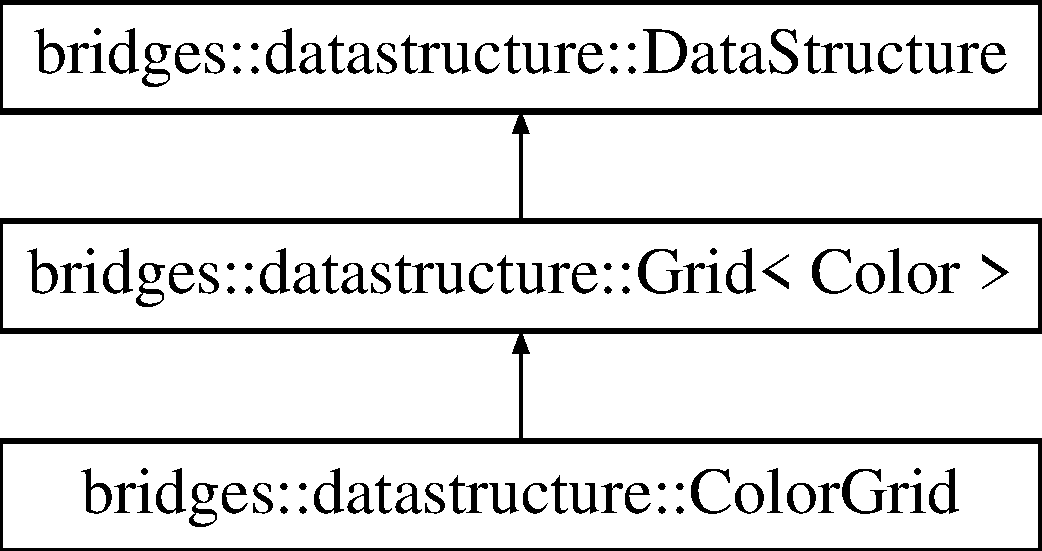
\includegraphics[height=3.000000cm]{classbridges_1_1datastructure_1_1_color_grid}
\end{center}
\end{figure}


\doxysubsection{Detailed Description}
This is a class in BRIDGES for representing an image. 

\begin{DoxyAuthor}{Author}
David Burlinson, Kalpathi Subramanian
\end{DoxyAuthor}
There is a tutorial about \mbox{\hyperlink{classbridges_1_1datastructure_1_1_color_grid}{Color\+Grid}} \+: \href{https://bridgesuncc.github.io/tutorials/Grid.html}{\texttt{ https\+://bridgesuncc.\+github.\+io/tutorials/\+Grid.\+html}} \doxysubsection*{Public Member Functions}
\begin{DoxyCompactItemize}
\item 
virtual const string \mbox{\hyperlink{classbridges_1_1datastructure_1_1_color_grid_afad945d648b427ca183a1dface8249b7}{get\+DStype}} () const override
\begin{DoxyCompactList}\small\item\em Return the data structure type. \end{DoxyCompactList}\item 
\mbox{\hyperlink{classbridges_1_1datastructure_1_1_color_grid_afe6bd7f8bf0dddd889ad7b6c159e928a}{Color\+Grid}} ()
\item 
\mbox{\hyperlink{classbridges_1_1datastructure_1_1_color_grid_a96a8df5eab72fb32c358ba12f2d4483b}{Color\+Grid}} (int rows, int cols)
\item 
\mbox{\hyperlink{classbridges_1_1datastructure_1_1_color_grid_a28f65f52274748d314ee47089e961c2c}{Color\+Grid}} (int rows, int cols, \mbox{\hyperlink{classbridges_1_1datastructure_1_1_color}{Color}} color)
\item 
\mbox{\hyperlink{classbridges_1_1datastructure_1_1_color_grid_adf9b21649638aec97394825d6d09f34c}{Color\+Grid}} (const \mbox{\hyperlink{classbridges_1_1datastructure_1_1_color_grid}{Color\+Grid}} \&cg)
\item 
\mbox{\hyperlink{classbridges_1_1datastructure_1_1_color_grid}{Color\+Grid}} \& \mbox{\hyperlink{classbridges_1_1datastructure_1_1_color_grid_abb8b358357bdccbd22fea5cea4a9862e}{operator=}} (const \mbox{\hyperlink{classbridges_1_1datastructure_1_1_color_grid}{Color\+Grid}} \&cg)
\item 
int \mbox{\hyperlink{classbridges_1_1datastructure_1_1_color_grid_ab437905ec904f941cd58d3393c3a5700}{get\+Height}} ()
\item 
int \mbox{\hyperlink{classbridges_1_1datastructure_1_1_color_grid_a46b358c31927e34f2068202e0cc23ae0}{get\+Width}} ()
\end{DoxyCompactItemize}
\doxysubsection*{Additional Inherited Members}


\doxysubsection{Constructor \& Destructor Documentation}
\mbox{\Hypertarget{classbridges_1_1datastructure_1_1_color_grid_afe6bd7f8bf0dddd889ad7b6c159e928a}\label{classbridges_1_1datastructure_1_1_color_grid_afe6bd7f8bf0dddd889ad7b6c159e928a}} 
\index{bridges::datastructure::ColorGrid@{bridges::datastructure::ColorGrid}!ColorGrid@{ColorGrid}}
\index{ColorGrid@{ColorGrid}!bridges::datastructure::ColorGrid@{bridges::datastructure::ColorGrid}}
\doxysubsubsection{\texorpdfstring{ColorGrid()}{ColorGrid()}\hspace{0.1cm}{\footnotesize\ttfamily [1/4]}}
{\footnotesize\ttfamily bridges\+::datastructure\+::\+Color\+Grid\+::\+Color\+Grid (\begin{DoxyParamCaption}{ }\end{DoxyParamCaption})\hspace{0.3cm}{\ttfamily [inline]}}

\mbox{\hyperlink{classbridges_1_1datastructure_1_1_color_grid}{Color\+Grid}} constructors \mbox{\Hypertarget{classbridges_1_1datastructure_1_1_color_grid_a96a8df5eab72fb32c358ba12f2d4483b}\label{classbridges_1_1datastructure_1_1_color_grid_a96a8df5eab72fb32c358ba12f2d4483b}} 
\index{bridges::datastructure::ColorGrid@{bridges::datastructure::ColorGrid}!ColorGrid@{ColorGrid}}
\index{ColorGrid@{ColorGrid}!bridges::datastructure::ColorGrid@{bridges::datastructure::ColorGrid}}
\doxysubsubsection{\texorpdfstring{ColorGrid()}{ColorGrid()}\hspace{0.1cm}{\footnotesize\ttfamily [2/4]}}
{\footnotesize\ttfamily bridges\+::datastructure\+::\+Color\+Grid\+::\+Color\+Grid (\begin{DoxyParamCaption}\item[{int}]{rows,  }\item[{int}]{cols }\end{DoxyParamCaption})\hspace{0.3cm}{\ttfamily [inline]}}

\mbox{\hyperlink{classbridges_1_1datastructure_1_1_grid}{Grid}} constructor with size arguments


\begin{DoxyParams}{Parameters}
{\em rows} & the number of rows of the grid \\
\hline
{\em cols} & the number of columns of the grid \\
\hline
\end{DoxyParams}
\mbox{\Hypertarget{classbridges_1_1datastructure_1_1_color_grid_a28f65f52274748d314ee47089e961c2c}\label{classbridges_1_1datastructure_1_1_color_grid_a28f65f52274748d314ee47089e961c2c}} 
\index{bridges::datastructure::ColorGrid@{bridges::datastructure::ColorGrid}!ColorGrid@{ColorGrid}}
\index{ColorGrid@{ColorGrid}!bridges::datastructure::ColorGrid@{bridges::datastructure::ColorGrid}}
\doxysubsubsection{\texorpdfstring{ColorGrid()}{ColorGrid()}\hspace{0.1cm}{\footnotesize\ttfamily [3/4]}}
{\footnotesize\ttfamily bridges\+::datastructure\+::\+Color\+Grid\+::\+Color\+Grid (\begin{DoxyParamCaption}\item[{int}]{rows,  }\item[{int}]{cols,  }\item[{\mbox{\hyperlink{classbridges_1_1datastructure_1_1_color}{Color}}}]{color }\end{DoxyParamCaption})\hspace{0.3cm}{\ttfamily [inline]}}

\mbox{\hyperlink{classbridges_1_1datastructure_1_1_grid}{Grid}} constructor with size and color string argument


\begin{DoxyParams}{Parameters}
{\em rows} & -\/ int representing the number of rows of the grid \\
\hline
{\em cols} & -\/ int representing the number of columns of the grid \\
\hline
{\em color} & -\/ \mbox{\hyperlink{classbridges_1_1datastructure_1_1_color}{Color}} object to use as default color \\
\hline
\end{DoxyParams}
\mbox{\Hypertarget{classbridges_1_1datastructure_1_1_color_grid_adf9b21649638aec97394825d6d09f34c}\label{classbridges_1_1datastructure_1_1_color_grid_adf9b21649638aec97394825d6d09f34c}} 
\index{bridges::datastructure::ColorGrid@{bridges::datastructure::ColorGrid}!ColorGrid@{ColorGrid}}
\index{ColorGrid@{ColorGrid}!bridges::datastructure::ColorGrid@{bridges::datastructure::ColorGrid}}
\doxysubsubsection{\texorpdfstring{ColorGrid()}{ColorGrid()}\hspace{0.1cm}{\footnotesize\ttfamily [4/4]}}
{\footnotesize\ttfamily bridges\+::datastructure\+::\+Color\+Grid\+::\+Color\+Grid (\begin{DoxyParamCaption}\item[{const \mbox{\hyperlink{classbridges_1_1datastructure_1_1_color_grid}{Color\+Grid}} \&}]{cg }\end{DoxyParamCaption})\hspace{0.3cm}{\ttfamily [inline]}}

Copy Constructor 

\doxysubsection{Member Function Documentation}
\mbox{\Hypertarget{classbridges_1_1datastructure_1_1_color_grid_afad945d648b427ca183a1dface8249b7}\label{classbridges_1_1datastructure_1_1_color_grid_afad945d648b427ca183a1dface8249b7}} 
\index{bridges::datastructure::ColorGrid@{bridges::datastructure::ColorGrid}!getDStype@{getDStype}}
\index{getDStype@{getDStype}!bridges::datastructure::ColorGrid@{bridges::datastructure::ColorGrid}}
\doxysubsubsection{\texorpdfstring{getDStype()}{getDStype()}}
{\footnotesize\ttfamily virtual const string bridges\+::datastructure\+::\+Color\+Grid\+::get\+DStype (\begin{DoxyParamCaption}{ }\end{DoxyParamCaption}) const\hspace{0.3cm}{\ttfamily [inline]}, {\ttfamily [override]}, {\ttfamily [virtual]}}



Return the data structure type. 

\begin{DoxyReturn}{Returns}
grid type (string) 
\end{DoxyReturn}


Reimplemented from \mbox{\hyperlink{classbridges_1_1datastructure_1_1_grid_a16aeae38446b96f440dea15f2b19334d}{bridges\+::datastructure\+::\+Grid$<$ Color $>$}}.

\mbox{\Hypertarget{classbridges_1_1datastructure_1_1_color_grid_ab437905ec904f941cd58d3393c3a5700}\label{classbridges_1_1datastructure_1_1_color_grid_ab437905ec904f941cd58d3393c3a5700}} 
\index{bridges::datastructure::ColorGrid@{bridges::datastructure::ColorGrid}!getHeight@{getHeight}}
\index{getHeight@{getHeight}!bridges::datastructure::ColorGrid@{bridges::datastructure::ColorGrid}}
\doxysubsubsection{\texorpdfstring{getHeight()}{getHeight()}}
{\footnotesize\ttfamily int bridges\+::datastructure\+::\+Color\+Grid\+::get\+Height (\begin{DoxyParamCaption}{ }\end{DoxyParamCaption})\hspace{0.3cm}{\ttfamily [inline]}}

Get the height of the color grid

\begin{DoxyReturn}{Returns}
the height (number of rows) of the grid 
\end{DoxyReturn}
\mbox{\Hypertarget{classbridges_1_1datastructure_1_1_color_grid_a46b358c31927e34f2068202e0cc23ae0}\label{classbridges_1_1datastructure_1_1_color_grid_a46b358c31927e34f2068202e0cc23ae0}} 
\index{bridges::datastructure::ColorGrid@{bridges::datastructure::ColorGrid}!getWidth@{getWidth}}
\index{getWidth@{getWidth}!bridges::datastructure::ColorGrid@{bridges::datastructure::ColorGrid}}
\doxysubsubsection{\texorpdfstring{getWidth()}{getWidth()}}
{\footnotesize\ttfamily int bridges\+::datastructure\+::\+Color\+Grid\+::get\+Width (\begin{DoxyParamCaption}{ }\end{DoxyParamCaption})\hspace{0.3cm}{\ttfamily [inline]}}

Get the width of the color grid

\begin{DoxyReturn}{Returns}
the width (number of columns) of the grid 
\end{DoxyReturn}
\mbox{\Hypertarget{classbridges_1_1datastructure_1_1_color_grid_abb8b358357bdccbd22fea5cea4a9862e}\label{classbridges_1_1datastructure_1_1_color_grid_abb8b358357bdccbd22fea5cea4a9862e}} 
\index{bridges::datastructure::ColorGrid@{bridges::datastructure::ColorGrid}!operator=@{operator=}}
\index{operator=@{operator=}!bridges::datastructure::ColorGrid@{bridges::datastructure::ColorGrid}}
\doxysubsubsection{\texorpdfstring{operator=()}{operator=()}}
{\footnotesize\ttfamily \mbox{\hyperlink{classbridges_1_1datastructure_1_1_color_grid}{Color\+Grid}}\& bridges\+::datastructure\+::\+Color\+Grid\+::operator= (\begin{DoxyParamCaption}\item[{const \mbox{\hyperlink{classbridges_1_1datastructure_1_1_color_grid}{Color\+Grid}} \&}]{cg }\end{DoxyParamCaption})\hspace{0.3cm}{\ttfamily [inline]}}



The documentation for this class was generated from the following file\+:\begin{DoxyCompactItemize}
\item 
/home/erik/work/bridges/bridges-\/cxx/src/\mbox{\hyperlink{_color_grid_8h}{Color\+Grid.\+h}}\end{DoxyCompactItemize}

\hypertarget{classbridges_1_1datastructure_1_1_array1_d_1_1const__iterator}{}\section{bridges\+:\+:datastructure\+:\+:Array1D$<$ E $>$\+:\+:const\+\_\+iterator Class Reference}
\label{classbridges_1_1datastructure_1_1_array1_d_1_1const__iterator}\index{bridges\+::datastructure\+::\+Array1\+D$<$ E $>$\+::const\+\_\+iterator@{bridges\+::datastructure\+::\+Array1\+D$<$ E $>$\+::const\+\_\+iterator}}


{\ttfamily \#include $<$Array1\+D.\+h$>$}



\subsection{Detailed Description}
\subsubsection*{template$<$typename E$>$\newline
class bridges\+::datastructure\+::\+Array1\+D$<$ E $>$\+::const\+\_\+iterator}

enabling iterator loops in const contexts \subsection*{Public Member Functions}
\begin{DoxyCompactItemize}
\item 
\mbox{\hyperlink{classbridges_1_1datastructure_1_1_array1_d_1_1const__iterator_a1ea421b46a3f0907190a91752e1f5b32}{const\+\_\+iterator}} (\mbox{\hyperlink{classbridges_1_1datastructure_1_1_array1_d}{Array1D}}$<$ E $>$ const \&a, int ind)
\item 
E const  \& \mbox{\hyperlink{classbridges_1_1datastructure_1_1_array1_d_1_1const__iterator_aec062ef1375b53092b872838c415081f}{operator$\ast$}} () const
\item 
\mbox{\hyperlink{classbridges_1_1datastructure_1_1_array1_d_1_1const__iterator}{const\+\_\+iterator}} \& \mbox{\hyperlink{classbridges_1_1datastructure_1_1_array1_d_1_1const__iterator_a754c1601b52473d4c8abc5e20af62b81}{operator++}} ()
\item 
\mbox{\hyperlink{classbridges_1_1datastructure_1_1_array1_d_1_1const__iterator}{const\+\_\+iterator}} \& \mbox{\hyperlink{classbridges_1_1datastructure_1_1_array1_d_1_1const__iterator_a700c9de64036c2cb61836e1ddc23cc1c}{operator-\/-\/}} ()
\item 
\mbox{\hyperlink{classbridges_1_1datastructure_1_1_array1_d_1_1const__iterator}{const\+\_\+iterator}} \& \mbox{\hyperlink{classbridges_1_1datastructure_1_1_array1_d_1_1const__iterator_aa7eb1bbe97e8f3257dc7d850be8f5937}{operator++}} (int)
\item 
\mbox{\hyperlink{classbridges_1_1datastructure_1_1_array1_d_1_1const__iterator}{const\+\_\+iterator}} \& \mbox{\hyperlink{classbridges_1_1datastructure_1_1_array1_d_1_1const__iterator_a815972df8b28780f88dac8133322e8ab}{operator-\/-\/}} (int)
\item 
bool \mbox{\hyperlink{classbridges_1_1datastructure_1_1_array1_d_1_1const__iterator_a004eca869afdc913a1d1a448bb4b7871}{operator==}} (const \mbox{\hyperlink{classbridges_1_1datastructure_1_1_array1_d_1_1const__iterator}{const\+\_\+iterator}} \&it) const
\item 
bool \mbox{\hyperlink{classbridges_1_1datastructure_1_1_array1_d_1_1const__iterator_ada463ec150271769b2a9e34c9bebdd05}{operator!=}} (const \mbox{\hyperlink{classbridges_1_1datastructure_1_1_array1_d_1_1const__iterator}{const\+\_\+iterator}} \&it) const
\end{DoxyCompactItemize}


\subsection{Constructor \& Destructor Documentation}
\mbox{\Hypertarget{classbridges_1_1datastructure_1_1_array1_d_1_1const__iterator_a1ea421b46a3f0907190a91752e1f5b32}\label{classbridges_1_1datastructure_1_1_array1_d_1_1const__iterator_a1ea421b46a3f0907190a91752e1f5b32}} 
\index{bridges\+::datastructure\+::\+Array1\+D\+::const\+\_\+iterator@{bridges\+::datastructure\+::\+Array1\+D\+::const\+\_\+iterator}!const\+\_\+iterator@{const\+\_\+iterator}}
\index{const\+\_\+iterator@{const\+\_\+iterator}!bridges\+::datastructure\+::\+Array1\+D\+::const\+\_\+iterator@{bridges\+::datastructure\+::\+Array1\+D\+::const\+\_\+iterator}}
\subsubsection{\texorpdfstring{const\+\_\+iterator()}{const\_iterator()}}
{\footnotesize\ttfamily template$<$typename E$>$ \\
\mbox{\hyperlink{classbridges_1_1datastructure_1_1_array1_d}{bridges\+::datastructure\+::\+Array1D}}$<$ E $>$\+::const\+\_\+iterator\+::const\+\_\+iterator (\begin{DoxyParamCaption}\item[{\mbox{\hyperlink{classbridges_1_1datastructure_1_1_array1_d}{Array1D}}$<$ E $>$ const \&}]{a,  }\item[{int}]{ind }\end{DoxyParamCaption})\hspace{0.3cm}{\ttfamily [inline]}}



\subsection{Member Function Documentation}
\mbox{\Hypertarget{classbridges_1_1datastructure_1_1_array1_d_1_1const__iterator_ada463ec150271769b2a9e34c9bebdd05}\label{classbridges_1_1datastructure_1_1_array1_d_1_1const__iterator_ada463ec150271769b2a9e34c9bebdd05}} 
\index{bridges\+::datastructure\+::\+Array1\+D\+::const\+\_\+iterator@{bridges\+::datastructure\+::\+Array1\+D\+::const\+\_\+iterator}!operator"!=@{operator"!=}}
\index{operator"!=@{operator"!=}!bridges\+::datastructure\+::\+Array1\+D\+::const\+\_\+iterator@{bridges\+::datastructure\+::\+Array1\+D\+::const\+\_\+iterator}}
\subsubsection{\texorpdfstring{operator"!=()}{operator!=()}}
{\footnotesize\ttfamily template$<$typename E$>$ \\
bool \mbox{\hyperlink{classbridges_1_1datastructure_1_1_array1_d}{bridges\+::datastructure\+::\+Array1D}}$<$ E $>$\+::const\+\_\+iterator\+::operator!= (\begin{DoxyParamCaption}\item[{const \mbox{\hyperlink{classbridges_1_1datastructure_1_1_array1_d_1_1const__iterator}{const\+\_\+iterator}} \&}]{it }\end{DoxyParamCaption}) const\hspace{0.3cm}{\ttfamily [inline]}}

\mbox{\Hypertarget{classbridges_1_1datastructure_1_1_array1_d_1_1const__iterator_aec062ef1375b53092b872838c415081f}\label{classbridges_1_1datastructure_1_1_array1_d_1_1const__iterator_aec062ef1375b53092b872838c415081f}} 
\index{bridges\+::datastructure\+::\+Array1\+D\+::const\+\_\+iterator@{bridges\+::datastructure\+::\+Array1\+D\+::const\+\_\+iterator}!operator$\ast$@{operator$\ast$}}
\index{operator$\ast$@{operator$\ast$}!bridges\+::datastructure\+::\+Array1\+D\+::const\+\_\+iterator@{bridges\+::datastructure\+::\+Array1\+D\+::const\+\_\+iterator}}
\subsubsection{\texorpdfstring{operator$\ast$()}{operator*()}}
{\footnotesize\ttfamily template$<$typename E$>$ \\
E const\& \mbox{\hyperlink{classbridges_1_1datastructure_1_1_array1_d}{bridges\+::datastructure\+::\+Array1D}}$<$ E $>$\+::const\+\_\+iterator\+::operator$\ast$ (\begin{DoxyParamCaption}{ }\end{DoxyParamCaption}) const\hspace{0.3cm}{\ttfamily [inline]}}

\mbox{\Hypertarget{classbridges_1_1datastructure_1_1_array1_d_1_1const__iterator_a754c1601b52473d4c8abc5e20af62b81}\label{classbridges_1_1datastructure_1_1_array1_d_1_1const__iterator_a754c1601b52473d4c8abc5e20af62b81}} 
\index{bridges\+::datastructure\+::\+Array1\+D\+::const\+\_\+iterator@{bridges\+::datastructure\+::\+Array1\+D\+::const\+\_\+iterator}!operator++@{operator++}}
\index{operator++@{operator++}!bridges\+::datastructure\+::\+Array1\+D\+::const\+\_\+iterator@{bridges\+::datastructure\+::\+Array1\+D\+::const\+\_\+iterator}}
\subsubsection{\texorpdfstring{operator++()}{operator++()}\hspace{0.1cm}{\footnotesize\ttfamily [1/2]}}
{\footnotesize\ttfamily template$<$typename E$>$ \\
\mbox{\hyperlink{classbridges_1_1datastructure_1_1_array1_d_1_1const__iterator}{const\+\_\+iterator}}\& \mbox{\hyperlink{classbridges_1_1datastructure_1_1_array1_d}{bridges\+::datastructure\+::\+Array1D}}$<$ E $>$\+::const\+\_\+iterator\+::operator++ (\begin{DoxyParamCaption}{ }\end{DoxyParamCaption})\hspace{0.3cm}{\ttfamily [inline]}}

\mbox{\Hypertarget{classbridges_1_1datastructure_1_1_array1_d_1_1const__iterator_aa7eb1bbe97e8f3257dc7d850be8f5937}\label{classbridges_1_1datastructure_1_1_array1_d_1_1const__iterator_aa7eb1bbe97e8f3257dc7d850be8f5937}} 
\index{bridges\+::datastructure\+::\+Array1\+D\+::const\+\_\+iterator@{bridges\+::datastructure\+::\+Array1\+D\+::const\+\_\+iterator}!operator++@{operator++}}
\index{operator++@{operator++}!bridges\+::datastructure\+::\+Array1\+D\+::const\+\_\+iterator@{bridges\+::datastructure\+::\+Array1\+D\+::const\+\_\+iterator}}
\subsubsection{\texorpdfstring{operator++()}{operator++()}\hspace{0.1cm}{\footnotesize\ttfamily [2/2]}}
{\footnotesize\ttfamily template$<$typename E$>$ \\
\mbox{\hyperlink{classbridges_1_1datastructure_1_1_array1_d_1_1const__iterator}{const\+\_\+iterator}}\& \mbox{\hyperlink{classbridges_1_1datastructure_1_1_array1_d}{bridges\+::datastructure\+::\+Array1D}}$<$ E $>$\+::const\+\_\+iterator\+::operator++ (\begin{DoxyParamCaption}\item[{int}]{ }\end{DoxyParamCaption})\hspace{0.3cm}{\ttfamily [inline]}}

\mbox{\Hypertarget{classbridges_1_1datastructure_1_1_array1_d_1_1const__iterator_a700c9de64036c2cb61836e1ddc23cc1c}\label{classbridges_1_1datastructure_1_1_array1_d_1_1const__iterator_a700c9de64036c2cb61836e1ddc23cc1c}} 
\index{bridges\+::datastructure\+::\+Array1\+D\+::const\+\_\+iterator@{bridges\+::datastructure\+::\+Array1\+D\+::const\+\_\+iterator}!operator-\/-\/@{operator-\/-\/}}
\index{operator-\/-\/@{operator-\/-\/}!bridges\+::datastructure\+::\+Array1\+D\+::const\+\_\+iterator@{bridges\+::datastructure\+::\+Array1\+D\+::const\+\_\+iterator}}
\subsubsection{\texorpdfstring{operator-\/-\/()}{operator--()}\hspace{0.1cm}{\footnotesize\ttfamily [1/2]}}
{\footnotesize\ttfamily template$<$typename E$>$ \\
\mbox{\hyperlink{classbridges_1_1datastructure_1_1_array1_d_1_1const__iterator}{const\+\_\+iterator}}\& \mbox{\hyperlink{classbridges_1_1datastructure_1_1_array1_d}{bridges\+::datastructure\+::\+Array1D}}$<$ E $>$\+::const\+\_\+iterator\+::operator-\/-\/ (\begin{DoxyParamCaption}{ }\end{DoxyParamCaption})\hspace{0.3cm}{\ttfamily [inline]}}

\mbox{\Hypertarget{classbridges_1_1datastructure_1_1_array1_d_1_1const__iterator_a815972df8b28780f88dac8133322e8ab}\label{classbridges_1_1datastructure_1_1_array1_d_1_1const__iterator_a815972df8b28780f88dac8133322e8ab}} 
\index{bridges\+::datastructure\+::\+Array1\+D\+::const\+\_\+iterator@{bridges\+::datastructure\+::\+Array1\+D\+::const\+\_\+iterator}!operator-\/-\/@{operator-\/-\/}}
\index{operator-\/-\/@{operator-\/-\/}!bridges\+::datastructure\+::\+Array1\+D\+::const\+\_\+iterator@{bridges\+::datastructure\+::\+Array1\+D\+::const\+\_\+iterator}}
\subsubsection{\texorpdfstring{operator-\/-\/()}{operator--()}\hspace{0.1cm}{\footnotesize\ttfamily [2/2]}}
{\footnotesize\ttfamily template$<$typename E$>$ \\
\mbox{\hyperlink{classbridges_1_1datastructure_1_1_array1_d_1_1const__iterator}{const\+\_\+iterator}}\& \mbox{\hyperlink{classbridges_1_1datastructure_1_1_array1_d}{bridges\+::datastructure\+::\+Array1D}}$<$ E $>$\+::const\+\_\+iterator\+::operator-\/-\/ (\begin{DoxyParamCaption}\item[{int}]{ }\end{DoxyParamCaption})\hspace{0.3cm}{\ttfamily [inline]}}

\mbox{\Hypertarget{classbridges_1_1datastructure_1_1_array1_d_1_1const__iterator_a004eca869afdc913a1d1a448bb4b7871}\label{classbridges_1_1datastructure_1_1_array1_d_1_1const__iterator_a004eca869afdc913a1d1a448bb4b7871}} 
\index{bridges\+::datastructure\+::\+Array1\+D\+::const\+\_\+iterator@{bridges\+::datastructure\+::\+Array1\+D\+::const\+\_\+iterator}!operator==@{operator==}}
\index{operator==@{operator==}!bridges\+::datastructure\+::\+Array1\+D\+::const\+\_\+iterator@{bridges\+::datastructure\+::\+Array1\+D\+::const\+\_\+iterator}}
\subsubsection{\texorpdfstring{operator==()}{operator==()}}
{\footnotesize\ttfamily template$<$typename E$>$ \\
bool \mbox{\hyperlink{classbridges_1_1datastructure_1_1_array1_d}{bridges\+::datastructure\+::\+Array1D}}$<$ E $>$\+::const\+\_\+iterator\+::operator== (\begin{DoxyParamCaption}\item[{const \mbox{\hyperlink{classbridges_1_1datastructure_1_1_array1_d_1_1const__iterator}{const\+\_\+iterator}} \&}]{it }\end{DoxyParamCaption}) const\hspace{0.3cm}{\ttfamily [inline]}}



The documentation for this class was generated from the following file\+:\begin{DoxyCompactItemize}
\item 
/\+Users/kalpathi/gr/bridges/client/cxx/src/\mbox{\hyperlink{_array1_d_8h}{Array1\+D.\+h}}\end{DoxyCompactItemize}

\hypertarget{classbridges_1_1datastructure_1_1_graph_adj_list_1_1_key_set__helper_1_1const__iterator}{}\doxysection{bridges\+::datastructure\+::Graph\+Adj\+List$<$ K, E1, E2 $>$\+::Key\+Set\+\_\+helper\+::const\+\_\+iterator Class Reference}
\label{classbridges_1_1datastructure_1_1_graph_adj_list_1_1_key_set__helper_1_1const__iterator}\index{bridges::datastructure::GraphAdjList$<$ K, E1, E2 $>$::KeySet\_helper::const\_iterator@{bridges::datastructure::GraphAdjList$<$ K, E1, E2 $>$::KeySet\_helper::const\_iterator}}


{\ttfamily \#include $<$Graph\+Adj\+List.\+h$>$}

\doxysubsection*{Public Member Functions}
\begin{DoxyCompactItemize}
\item 
\mbox{\hyperlink{classbridges_1_1datastructure_1_1_graph_adj_list_1_1_key_set__helper_1_1const__iterator_a028172e70957f093f02ee95c77d89392}{const\+\_\+iterator}} (typename std\+::unordered\+\_\+map$<$ K, \mbox{\hyperlink{classbridges_1_1datastructure_1_1_element}{Element}}$<$ E1 $>$ $\ast$ $>$\+::\mbox{\hyperlink{classbridges_1_1datastructure_1_1_graph_adj_list_1_1_key_set__helper_1_1const__iterator}{const\+\_\+iterator}} i)
\item 
bool \mbox{\hyperlink{classbridges_1_1datastructure_1_1_graph_adj_list_1_1_key_set__helper_1_1const__iterator_a373e0c206d63dfda41108ebfcfae5fe8}{operator!=}} (const \mbox{\hyperlink{classbridges_1_1datastructure_1_1_graph_adj_list_1_1_key_set__helper_1_1const__iterator}{const\+\_\+iterator}} \&it) const
\item 
const K \& \mbox{\hyperlink{classbridges_1_1datastructure_1_1_graph_adj_list_1_1_key_set__helper_1_1const__iterator_a8369373435ffc6d6bfb3d5d5da13eea3}{operator$\ast$}} () const
\item 
\mbox{\hyperlink{classbridges_1_1datastructure_1_1_graph_adj_list_1_1_key_set__helper_1_1const__iterator}{const\+\_\+iterator}} \& \mbox{\hyperlink{classbridges_1_1datastructure_1_1_graph_adj_list_1_1_key_set__helper_1_1const__iterator_acbeb342b54bfdb8ece520e9d5cbf66db}{operator++}} ()
\end{DoxyCompactItemize}


\doxysubsection{Constructor \& Destructor Documentation}
\mbox{\Hypertarget{classbridges_1_1datastructure_1_1_graph_adj_list_1_1_key_set__helper_1_1const__iterator_a028172e70957f093f02ee95c77d89392}\label{classbridges_1_1datastructure_1_1_graph_adj_list_1_1_key_set__helper_1_1const__iterator_a028172e70957f093f02ee95c77d89392}} 
\index{bridges::datastructure::GraphAdjList$<$ K, E1, E2 $>$::KeySet\_helper::const\_iterator@{bridges::datastructure::GraphAdjList$<$ K, E1, E2 $>$::KeySet\_helper::const\_iterator}!const\_iterator@{const\_iterator}}
\index{const\_iterator@{const\_iterator}!bridges::datastructure::GraphAdjList$<$ K, E1, E2 $>$::KeySet\_helper::const\_iterator@{bridges::datastructure::GraphAdjList$<$ K, E1, E2 $>$::KeySet\_helper::const\_iterator}}
\doxysubsubsection{\texorpdfstring{const\_iterator()}{const\_iterator()}}
{\footnotesize\ttfamily template$<$typename K , typename E1  = K, typename E2  = E1$>$ \\
\mbox{\hyperlink{classbridges_1_1datastructure_1_1_graph_adj_list}{bridges\+::datastructure\+::\+Graph\+Adj\+List}}$<$ K, E1, E2 $>$\+::Key\+Set\+\_\+helper\+::const\+\_\+iterator\+::const\+\_\+iterator (\begin{DoxyParamCaption}\item[{typename std\+::unordered\+\_\+map$<$ K, \mbox{\hyperlink{classbridges_1_1datastructure_1_1_element}{Element}}$<$ E1 $>$ $\ast$ $>$\+::\mbox{\hyperlink{classbridges_1_1datastructure_1_1_graph_adj_list_1_1_key_set__helper_1_1const__iterator}{const\+\_\+iterator}}}]{i }\end{DoxyParamCaption})\hspace{0.3cm}{\ttfamily [inline]}}



\doxysubsection{Member Function Documentation}
\mbox{\Hypertarget{classbridges_1_1datastructure_1_1_graph_adj_list_1_1_key_set__helper_1_1const__iterator_a373e0c206d63dfda41108ebfcfae5fe8}\label{classbridges_1_1datastructure_1_1_graph_adj_list_1_1_key_set__helper_1_1const__iterator_a373e0c206d63dfda41108ebfcfae5fe8}} 
\index{bridges::datastructure::GraphAdjList$<$ K, E1, E2 $>$::KeySet\_helper::const\_iterator@{bridges::datastructure::GraphAdjList$<$ K, E1, E2 $>$::KeySet\_helper::const\_iterator}!operator"!=@{operator"!=}}
\index{operator"!=@{operator"!=}!bridges::datastructure::GraphAdjList$<$ K, E1, E2 $>$::KeySet\_helper::const\_iterator@{bridges::datastructure::GraphAdjList$<$ K, E1, E2 $>$::KeySet\_helper::const\_iterator}}
\doxysubsubsection{\texorpdfstring{operator"!=()}{operator!=()}}
{\footnotesize\ttfamily template$<$typename K , typename E1  = K, typename E2  = E1$>$ \\
bool \mbox{\hyperlink{classbridges_1_1datastructure_1_1_graph_adj_list}{bridges\+::datastructure\+::\+Graph\+Adj\+List}}$<$ K, E1, E2 $>$\+::Key\+Set\+\_\+helper\+::const\+\_\+iterator\+::operator!= (\begin{DoxyParamCaption}\item[{const \mbox{\hyperlink{classbridges_1_1datastructure_1_1_graph_adj_list_1_1_key_set__helper_1_1const__iterator}{const\+\_\+iterator}} \&}]{it }\end{DoxyParamCaption}) const\hspace{0.3cm}{\ttfamily [inline]}}

\mbox{\Hypertarget{classbridges_1_1datastructure_1_1_graph_adj_list_1_1_key_set__helper_1_1const__iterator_a8369373435ffc6d6bfb3d5d5da13eea3}\label{classbridges_1_1datastructure_1_1_graph_adj_list_1_1_key_set__helper_1_1const__iterator_a8369373435ffc6d6bfb3d5d5da13eea3}} 
\index{bridges::datastructure::GraphAdjList$<$ K, E1, E2 $>$::KeySet\_helper::const\_iterator@{bridges::datastructure::GraphAdjList$<$ K, E1, E2 $>$::KeySet\_helper::const\_iterator}!operator$\ast$@{operator$\ast$}}
\index{operator$\ast$@{operator$\ast$}!bridges::datastructure::GraphAdjList$<$ K, E1, E2 $>$::KeySet\_helper::const\_iterator@{bridges::datastructure::GraphAdjList$<$ K, E1, E2 $>$::KeySet\_helper::const\_iterator}}
\doxysubsubsection{\texorpdfstring{operator$\ast$()}{operator*()}}
{\footnotesize\ttfamily template$<$typename K , typename E1  = K, typename E2  = E1$>$ \\
const K\& \mbox{\hyperlink{classbridges_1_1datastructure_1_1_graph_adj_list}{bridges\+::datastructure\+::\+Graph\+Adj\+List}}$<$ K, E1, E2 $>$\+::Key\+Set\+\_\+helper\+::const\+\_\+iterator\+::operator$\ast$ (\begin{DoxyParamCaption}{ }\end{DoxyParamCaption}) const\hspace{0.3cm}{\ttfamily [inline]}}

\mbox{\Hypertarget{classbridges_1_1datastructure_1_1_graph_adj_list_1_1_key_set__helper_1_1const__iterator_acbeb342b54bfdb8ece520e9d5cbf66db}\label{classbridges_1_1datastructure_1_1_graph_adj_list_1_1_key_set__helper_1_1const__iterator_acbeb342b54bfdb8ece520e9d5cbf66db}} 
\index{bridges::datastructure::GraphAdjList$<$ K, E1, E2 $>$::KeySet\_helper::const\_iterator@{bridges::datastructure::GraphAdjList$<$ K, E1, E2 $>$::KeySet\_helper::const\_iterator}!operator++@{operator++}}
\index{operator++@{operator++}!bridges::datastructure::GraphAdjList$<$ K, E1, E2 $>$::KeySet\_helper::const\_iterator@{bridges::datastructure::GraphAdjList$<$ K, E1, E2 $>$::KeySet\_helper::const\_iterator}}
\doxysubsubsection{\texorpdfstring{operator++()}{operator++()}}
{\footnotesize\ttfamily template$<$typename K , typename E1  = K, typename E2  = E1$>$ \\
\mbox{\hyperlink{classbridges_1_1datastructure_1_1_graph_adj_list_1_1_key_set__helper_1_1const__iterator}{const\+\_\+iterator}}\& \mbox{\hyperlink{classbridges_1_1datastructure_1_1_graph_adj_list}{bridges\+::datastructure\+::\+Graph\+Adj\+List}}$<$ K, E1, E2 $>$\+::Key\+Set\+\_\+helper\+::const\+\_\+iterator\+::operator++ (\begin{DoxyParamCaption}{ }\end{DoxyParamCaption})\hspace{0.3cm}{\ttfamily [inline]}}



The documentation for this class was generated from the following file\+:\begin{DoxyCompactItemize}
\item 
/home/erik/work/bridges/bridges-\/cxx/src/\mbox{\hyperlink{_graph_adj_list_8h}{Graph\+Adj\+List.\+h}}\end{DoxyCompactItemize}

\hypertarget{classbridges_1_1datastructure_1_1_graph_adj_list_1_1_vertex_element_set__listhelper_1_1const__iterator}{}\section{bridges\+::datastructure\+::Graph\+Adj\+List$<$ K, E1, E2 $>$\+::Vertex\+Element\+Set\+\_\+listhelper\+::const\+\_\+iterator Class Reference}
\label{classbridges_1_1datastructure_1_1_graph_adj_list_1_1_vertex_element_set__listhelper_1_1const__iterator}\index{bridges::datastructure::GraphAdjList$<$ K, E1, E2 $>$::VertexElementSet\_listhelper::const\_iterator@{bridges::datastructure::GraphAdjList$<$ K, E1, E2 $>$::VertexElementSet\_listhelper::const\_iterator}}


{\ttfamily \#include $<$Graph\+Adj\+List.\+h$>$}



\subsection{Detailed Description}
\subsubsection*{template$<$typename K, typename E1 = K, typename E2 = E1$>$\newline
class bridges\+::datastructure\+::\+Graph\+Adj\+List$<$ K, E1, E2 $>$\+::\+Vertex\+Element\+Set\+\_\+listhelper\+::const\+\_\+iterator}

This is a helper class to return sets of vertices in a way that are iterable with range for loops. Students should have to use this directly. \subsection*{Public Member Functions}
\begin{DoxyCompactItemize}
\item 
\mbox{\hyperlink{classbridges_1_1datastructure_1_1_graph_adj_list_1_1_vertex_element_set__listhelper_1_1const__iterator_a023fa89f9e79573104de174f5fbab487}{const\+\_\+iterator}} (typename std\+::unordered\+\_\+map$<$ K, \mbox{\hyperlink{classbridges_1_1datastructure_1_1_element}{Element}}$<$ E1 $>$ $\ast$ $>$\+::\mbox{\hyperlink{classbridges_1_1datastructure_1_1_graph_adj_list_1_1_vertex_element_set__listhelper_1_1const__iterator}{const\+\_\+iterator}} i)
\item 
bool \mbox{\hyperlink{classbridges_1_1datastructure_1_1_graph_adj_list_1_1_vertex_element_set__listhelper_1_1const__iterator_ac7ce05d2bf7491005acf6e4a668cea1b}{operator!=}} (const \mbox{\hyperlink{classbridges_1_1datastructure_1_1_graph_adj_list_1_1_vertex_element_set__listhelper_1_1const__iterator}{const\+\_\+iterator}} \&it) const
\item 
\mbox{\hyperlink{classbridges_1_1datastructure_1_1_element}{Element}}$<$ E1 $>$ const  $\ast$ \mbox{\hyperlink{classbridges_1_1datastructure_1_1_graph_adj_list_1_1_vertex_element_set__listhelper_1_1const__iterator_ac38dbc97be4bfd788306e827ab683211}{operator $\ast$}} () const
\item 
\mbox{\hyperlink{classbridges_1_1datastructure_1_1_graph_adj_list_1_1_vertex_element_set__listhelper_1_1const__iterator}{const\+\_\+iterator}} \& \mbox{\hyperlink{classbridges_1_1datastructure_1_1_graph_adj_list_1_1_vertex_element_set__listhelper_1_1const__iterator_ac1c6d4c3ab7486d648e469b1783f42df}{operator++}} ()
\end{DoxyCompactItemize}


\subsection{Constructor \& Destructor Documentation}
\mbox{\Hypertarget{classbridges_1_1datastructure_1_1_graph_adj_list_1_1_vertex_element_set__listhelper_1_1const__iterator_a023fa89f9e79573104de174f5fbab487}\label{classbridges_1_1datastructure_1_1_graph_adj_list_1_1_vertex_element_set__listhelper_1_1const__iterator_a023fa89f9e79573104de174f5fbab487}} 
\index{bridges::datastructure::GraphAdjList$<$ K, E1, E2 $>$::VertexElementSet\_listhelper::const\_iterator@{bridges::datastructure::GraphAdjList$<$ K, E1, E2 $>$::VertexElementSet\_listhelper::const\_iterator}!const\_iterator@{const\_iterator}}
\index{const\_iterator@{const\_iterator}!bridges::datastructure::GraphAdjList$<$ K, E1, E2 $>$::VertexElementSet\_listhelper::const\_iterator@{bridges::datastructure::GraphAdjList$<$ K, E1, E2 $>$::VertexElementSet\_listhelper::const\_iterator}}
\subsubsection{\texorpdfstring{const\_iterator()}{const\_iterator()}}
{\footnotesize\ttfamily template$<$typename K, typename E1 = K, typename E2 = E1$>$ \\
\mbox{\hyperlink{classbridges_1_1datastructure_1_1_graph_adj_list}{bridges\+::datastructure\+::\+Graph\+Adj\+List}}$<$ K, E1, E2 $>$\+::Vertex\+Element\+Set\+\_\+listhelper\+::const\+\_\+iterator\+::const\+\_\+iterator (\begin{DoxyParamCaption}\item[{typename std\+::unordered\+\_\+map$<$ K, \mbox{\hyperlink{classbridges_1_1datastructure_1_1_element}{Element}}$<$ E1 $>$ $\ast$ $>$\+::\mbox{\hyperlink{classbridges_1_1datastructure_1_1_graph_adj_list_1_1_vertex_element_set__listhelper_1_1const__iterator}{const\+\_\+iterator}}}]{i }\end{DoxyParamCaption})\hspace{0.3cm}{\ttfamily [inline]}}



\subsection{Member Function Documentation}
\mbox{\Hypertarget{classbridges_1_1datastructure_1_1_graph_adj_list_1_1_vertex_element_set__listhelper_1_1const__iterator_ac38dbc97be4bfd788306e827ab683211}\label{classbridges_1_1datastructure_1_1_graph_adj_list_1_1_vertex_element_set__listhelper_1_1const__iterator_ac38dbc97be4bfd788306e827ab683211}} 
\index{bridges::datastructure::GraphAdjList$<$ K, E1, E2 $>$::VertexElementSet\_listhelper::const\_iterator@{bridges::datastructure::GraphAdjList$<$ K, E1, E2 $>$::VertexElementSet\_listhelper::const\_iterator}!operator $\ast$@{operator $\ast$}}
\index{operator $\ast$@{operator $\ast$}!bridges::datastructure::GraphAdjList$<$ K, E1, E2 $>$::VertexElementSet\_listhelper::const\_iterator@{bridges::datastructure::GraphAdjList$<$ K, E1, E2 $>$::VertexElementSet\_listhelper::const\_iterator}}
\subsubsection{\texorpdfstring{operator $\ast$()}{operator *()}}
{\footnotesize\ttfamily template$<$typename K, typename E1 = K, typename E2 = E1$>$ \\
\mbox{\hyperlink{classbridges_1_1datastructure_1_1_element}{Element}}$<$E1$>$ const$\ast$ \mbox{\hyperlink{classbridges_1_1datastructure_1_1_graph_adj_list}{bridges\+::datastructure\+::\+Graph\+Adj\+List}}$<$ K, E1, E2 $>$\+::Vertex\+Element\+Set\+\_\+listhelper\+::const\+\_\+iterator\+::operator $\ast$ (\begin{DoxyParamCaption}{ }\end{DoxyParamCaption}) const\hspace{0.3cm}{\ttfamily [inline]}}

\mbox{\Hypertarget{classbridges_1_1datastructure_1_1_graph_adj_list_1_1_vertex_element_set__listhelper_1_1const__iterator_ac7ce05d2bf7491005acf6e4a668cea1b}\label{classbridges_1_1datastructure_1_1_graph_adj_list_1_1_vertex_element_set__listhelper_1_1const__iterator_ac7ce05d2bf7491005acf6e4a668cea1b}} 
\index{bridges::datastructure::GraphAdjList$<$ K, E1, E2 $>$::VertexElementSet\_listhelper::const\_iterator@{bridges::datastructure::GraphAdjList$<$ K, E1, E2 $>$::VertexElementSet\_listhelper::const\_iterator}!operator"!=@{operator"!=}}
\index{operator"!=@{operator"!=}!bridges::datastructure::GraphAdjList$<$ K, E1, E2 $>$::VertexElementSet\_listhelper::const\_iterator@{bridges::datastructure::GraphAdjList$<$ K, E1, E2 $>$::VertexElementSet\_listhelper::const\_iterator}}
\subsubsection{\texorpdfstring{operator"!=()}{operator!=()}}
{\footnotesize\ttfamily template$<$typename K, typename E1 = K, typename E2 = E1$>$ \\
bool \mbox{\hyperlink{classbridges_1_1datastructure_1_1_graph_adj_list}{bridges\+::datastructure\+::\+Graph\+Adj\+List}}$<$ K, E1, E2 $>$\+::Vertex\+Element\+Set\+\_\+listhelper\+::const\+\_\+iterator\+::operator!= (\begin{DoxyParamCaption}\item[{const \mbox{\hyperlink{classbridges_1_1datastructure_1_1_graph_adj_list_1_1_vertex_element_set__listhelper_1_1const__iterator}{const\+\_\+iterator}} \&}]{it }\end{DoxyParamCaption}) const\hspace{0.3cm}{\ttfamily [inline]}}

\mbox{\Hypertarget{classbridges_1_1datastructure_1_1_graph_adj_list_1_1_vertex_element_set__listhelper_1_1const__iterator_ac1c6d4c3ab7486d648e469b1783f42df}\label{classbridges_1_1datastructure_1_1_graph_adj_list_1_1_vertex_element_set__listhelper_1_1const__iterator_ac1c6d4c3ab7486d648e469b1783f42df}} 
\index{bridges::datastructure::GraphAdjList$<$ K, E1, E2 $>$::VertexElementSet\_listhelper::const\_iterator@{bridges::datastructure::GraphAdjList$<$ K, E1, E2 $>$::VertexElementSet\_listhelper::const\_iterator}!operator++@{operator++}}
\index{operator++@{operator++}!bridges::datastructure::GraphAdjList$<$ K, E1, E2 $>$::VertexElementSet\_listhelper::const\_iterator@{bridges::datastructure::GraphAdjList$<$ K, E1, E2 $>$::VertexElementSet\_listhelper::const\_iterator}}
\subsubsection{\texorpdfstring{operator++()}{operator++()}}
{\footnotesize\ttfamily template$<$typename K, typename E1 = K, typename E2 = E1$>$ \\
\mbox{\hyperlink{classbridges_1_1datastructure_1_1_graph_adj_list_1_1_vertex_element_set__listhelper_1_1const__iterator}{const\+\_\+iterator}}\& \mbox{\hyperlink{classbridges_1_1datastructure_1_1_graph_adj_list}{bridges\+::datastructure\+::\+Graph\+Adj\+List}}$<$ K, E1, E2 $>$\+::Vertex\+Element\+Set\+\_\+listhelper\+::const\+\_\+iterator\+::operator++ (\begin{DoxyParamCaption}{ }\end{DoxyParamCaption})\hspace{0.3cm}{\ttfamily [inline]}}



The documentation for this class was generated from the following file\+:\begin{DoxyCompactItemize}
\item 
/\+Users/kalpathi/gr/bridges/cxx/src/\mbox{\hyperlink{_graph_adj_list_8h}{Graph\+Adj\+List.\+h}}\end{DoxyCompactItemize}

\hypertarget{classbridges_1_1datastructure_1_1_graph_adj_list_1_1const_vertex_element_set__listhelper_1_1const__iterator}{}\section{bridges\+:\+:datastructure\+:\+:Graph\+Adj\+List$<$ K, E1, E2 $>$\+:\+:const\+Vertex\+Element\+Set\+\_\+listhelper\+:\+:const\+\_\+iterator Class Reference}
\label{classbridges_1_1datastructure_1_1_graph_adj_list_1_1const_vertex_element_set__listhelper_1_1const__iterator}\index{bridges\+::datastructure\+::\+Graph\+Adj\+List$<$ K, E1, E2 $>$\+::const\+Vertex\+Element\+Set\+\_\+listhelper\+::const\+\_\+iterator@{bridges\+::datastructure\+::\+Graph\+Adj\+List$<$ K, E1, E2 $>$\+::const\+Vertex\+Element\+Set\+\_\+listhelper\+::const\+\_\+iterator}}


{\ttfamily \#include $<$Graph\+Adj\+List.\+h$>$}



\subsection{Detailed Description}
\subsubsection*{template$<$typename K, typename E1 = K, typename E2 = E1$>$\newline
class bridges\+::datastructure\+::\+Graph\+Adj\+List$<$ K, E1, E2 $>$\+::const\+Vertex\+Element\+Set\+\_\+listhelper\+::const\+\_\+iterator}

This is a helper class to return sets of vertices ina way that are iterable with range for loops. Students should not have to use this directly. \subsection*{Public Member Functions}
\begin{DoxyCompactItemize}
\item 
\mbox{\hyperlink{classbridges_1_1datastructure_1_1_graph_adj_list_1_1const_vertex_element_set__listhelper_1_1const__iterator_a4b7fc58222ec911d26672daa5e255a1d}{const\+\_\+iterator}} (typename std\+::unordered\+\_\+map$<$ K, \mbox{\hyperlink{classbridges_1_1datastructure_1_1_element}{Element}}$<$ E1 $>$ $\ast$ $>$\+::\mbox{\hyperlink{classbridges_1_1datastructure_1_1_graph_adj_list_1_1const_vertex_element_set__listhelper_1_1const__iterator}{const\+\_\+iterator}} i)
\item 
bool \mbox{\hyperlink{classbridges_1_1datastructure_1_1_graph_adj_list_1_1const_vertex_element_set__listhelper_1_1const__iterator_ac30d7d7e8eb8a976f7dd193bc7cb7b1c}{operator!=}} (const \mbox{\hyperlink{classbridges_1_1datastructure_1_1_graph_adj_list_1_1const_vertex_element_set__listhelper_1_1const__iterator}{const\+\_\+iterator}} \&it) const
\item 
\mbox{\hyperlink{classbridges_1_1datastructure_1_1_element}{Element}}$<$ E1 $>$ const  $\ast$ \mbox{\hyperlink{classbridges_1_1datastructure_1_1_graph_adj_list_1_1const_vertex_element_set__listhelper_1_1const__iterator_ae6e06df1132d7d1646385388d28bc8b0}{operator$\ast$}} () const
\item 
\mbox{\hyperlink{classbridges_1_1datastructure_1_1_graph_adj_list_1_1const_vertex_element_set__listhelper_1_1const__iterator}{const\+\_\+iterator}} \& \mbox{\hyperlink{classbridges_1_1datastructure_1_1_graph_adj_list_1_1const_vertex_element_set__listhelper_1_1const__iterator_ad778b5c8406c308e1b80700882171243}{operator++}} ()
\end{DoxyCompactItemize}


\subsection{Constructor \& Destructor Documentation}
\mbox{\Hypertarget{classbridges_1_1datastructure_1_1_graph_adj_list_1_1const_vertex_element_set__listhelper_1_1const__iterator_a4b7fc58222ec911d26672daa5e255a1d}\label{classbridges_1_1datastructure_1_1_graph_adj_list_1_1const_vertex_element_set__listhelper_1_1const__iterator_a4b7fc58222ec911d26672daa5e255a1d}} 
\index{bridges\+::datastructure\+::\+Graph\+Adj\+List\+::const\+Vertex\+Element\+Set\+\_\+listhelper\+::const\+\_\+iterator@{bridges\+::datastructure\+::\+Graph\+Adj\+List\+::const\+Vertex\+Element\+Set\+\_\+listhelper\+::const\+\_\+iterator}!const\+\_\+iterator@{const\+\_\+iterator}}
\index{const\+\_\+iterator@{const\+\_\+iterator}!bridges\+::datastructure\+::\+Graph\+Adj\+List\+::const\+Vertex\+Element\+Set\+\_\+listhelper\+::const\+\_\+iterator@{bridges\+::datastructure\+::\+Graph\+Adj\+List\+::const\+Vertex\+Element\+Set\+\_\+listhelper\+::const\+\_\+iterator}}
\subsubsection{\texorpdfstring{const\+\_\+iterator()}{const\_iterator()}}
{\footnotesize\ttfamily template$<$typename K, typename E1 = K, typename E2 = E1$>$ \\
\mbox{\hyperlink{classbridges_1_1datastructure_1_1_graph_adj_list}{bridges\+::datastructure\+::\+Graph\+Adj\+List}}$<$ K, E1, E2 $>$\+::const\+Vertex\+Element\+Set\+\_\+listhelper\+::const\+\_\+iterator\+::const\+\_\+iterator (\begin{DoxyParamCaption}\item[{typename std\+::unordered\+\_\+map$<$ K, \mbox{\hyperlink{classbridges_1_1datastructure_1_1_element}{Element}}$<$ E1 $>$ $\ast$ $>$\+::\mbox{\hyperlink{classbridges_1_1datastructure_1_1_graph_adj_list_1_1const_vertex_element_set__listhelper_1_1const__iterator}{const\+\_\+iterator}}}]{i }\end{DoxyParamCaption})\hspace{0.3cm}{\ttfamily [inline]}}



\subsection{Member Function Documentation}
\mbox{\Hypertarget{classbridges_1_1datastructure_1_1_graph_adj_list_1_1const_vertex_element_set__listhelper_1_1const__iterator_ac30d7d7e8eb8a976f7dd193bc7cb7b1c}\label{classbridges_1_1datastructure_1_1_graph_adj_list_1_1const_vertex_element_set__listhelper_1_1const__iterator_ac30d7d7e8eb8a976f7dd193bc7cb7b1c}} 
\index{bridges\+::datastructure\+::\+Graph\+Adj\+List\+::const\+Vertex\+Element\+Set\+\_\+listhelper\+::const\+\_\+iterator@{bridges\+::datastructure\+::\+Graph\+Adj\+List\+::const\+Vertex\+Element\+Set\+\_\+listhelper\+::const\+\_\+iterator}!operator"!=@{operator"!=}}
\index{operator"!=@{operator"!=}!bridges\+::datastructure\+::\+Graph\+Adj\+List\+::const\+Vertex\+Element\+Set\+\_\+listhelper\+::const\+\_\+iterator@{bridges\+::datastructure\+::\+Graph\+Adj\+List\+::const\+Vertex\+Element\+Set\+\_\+listhelper\+::const\+\_\+iterator}}
\subsubsection{\texorpdfstring{operator"!=()}{operator!=()}}
{\footnotesize\ttfamily template$<$typename K, typename E1 = K, typename E2 = E1$>$ \\
bool \mbox{\hyperlink{classbridges_1_1datastructure_1_1_graph_adj_list}{bridges\+::datastructure\+::\+Graph\+Adj\+List}}$<$ K, E1, E2 $>$\+::const\+Vertex\+Element\+Set\+\_\+listhelper\+::const\+\_\+iterator\+::operator!= (\begin{DoxyParamCaption}\item[{const \mbox{\hyperlink{classbridges_1_1datastructure_1_1_graph_adj_list_1_1const_vertex_element_set__listhelper_1_1const__iterator}{const\+\_\+iterator}} \&}]{it }\end{DoxyParamCaption}) const\hspace{0.3cm}{\ttfamily [inline]}}

\mbox{\Hypertarget{classbridges_1_1datastructure_1_1_graph_adj_list_1_1const_vertex_element_set__listhelper_1_1const__iterator_ae6e06df1132d7d1646385388d28bc8b0}\label{classbridges_1_1datastructure_1_1_graph_adj_list_1_1const_vertex_element_set__listhelper_1_1const__iterator_ae6e06df1132d7d1646385388d28bc8b0}} 
\index{bridges\+::datastructure\+::\+Graph\+Adj\+List\+::const\+Vertex\+Element\+Set\+\_\+listhelper\+::const\+\_\+iterator@{bridges\+::datastructure\+::\+Graph\+Adj\+List\+::const\+Vertex\+Element\+Set\+\_\+listhelper\+::const\+\_\+iterator}!operator$\ast$@{operator$\ast$}}
\index{operator$\ast$@{operator$\ast$}!bridges\+::datastructure\+::\+Graph\+Adj\+List\+::const\+Vertex\+Element\+Set\+\_\+listhelper\+::const\+\_\+iterator@{bridges\+::datastructure\+::\+Graph\+Adj\+List\+::const\+Vertex\+Element\+Set\+\_\+listhelper\+::const\+\_\+iterator}}
\subsubsection{\texorpdfstring{operator$\ast$()}{operator*()}}
{\footnotesize\ttfamily template$<$typename K, typename E1 = K, typename E2 = E1$>$ \\
\mbox{\hyperlink{classbridges_1_1datastructure_1_1_element}{Element}}$<$E1$>$ const$\ast$ \mbox{\hyperlink{classbridges_1_1datastructure_1_1_graph_adj_list}{bridges\+::datastructure\+::\+Graph\+Adj\+List}}$<$ K, E1, E2 $>$\+::const\+Vertex\+Element\+Set\+\_\+listhelper\+::const\+\_\+iterator\+::operator$\ast$ (\begin{DoxyParamCaption}{ }\end{DoxyParamCaption}) const\hspace{0.3cm}{\ttfamily [inline]}}

\mbox{\Hypertarget{classbridges_1_1datastructure_1_1_graph_adj_list_1_1const_vertex_element_set__listhelper_1_1const__iterator_ad778b5c8406c308e1b80700882171243}\label{classbridges_1_1datastructure_1_1_graph_adj_list_1_1const_vertex_element_set__listhelper_1_1const__iterator_ad778b5c8406c308e1b80700882171243}} 
\index{bridges\+::datastructure\+::\+Graph\+Adj\+List\+::const\+Vertex\+Element\+Set\+\_\+listhelper\+::const\+\_\+iterator@{bridges\+::datastructure\+::\+Graph\+Adj\+List\+::const\+Vertex\+Element\+Set\+\_\+listhelper\+::const\+\_\+iterator}!operator++@{operator++}}
\index{operator++@{operator++}!bridges\+::datastructure\+::\+Graph\+Adj\+List\+::const\+Vertex\+Element\+Set\+\_\+listhelper\+::const\+\_\+iterator@{bridges\+::datastructure\+::\+Graph\+Adj\+List\+::const\+Vertex\+Element\+Set\+\_\+listhelper\+::const\+\_\+iterator}}
\subsubsection{\texorpdfstring{operator++()}{operator++()}}
{\footnotesize\ttfamily template$<$typename K, typename E1 = K, typename E2 = E1$>$ \\
\mbox{\hyperlink{classbridges_1_1datastructure_1_1_graph_adj_list_1_1const_vertex_element_set__listhelper_1_1const__iterator}{const\+\_\+iterator}}\& \mbox{\hyperlink{classbridges_1_1datastructure_1_1_graph_adj_list}{bridges\+::datastructure\+::\+Graph\+Adj\+List}}$<$ K, E1, E2 $>$\+::const\+Vertex\+Element\+Set\+\_\+listhelper\+::const\+\_\+iterator\+::operator++ (\begin{DoxyParamCaption}{ }\end{DoxyParamCaption})\hspace{0.3cm}{\ttfamily [inline]}}



The documentation for this class was generated from the following file\+:\begin{DoxyCompactItemize}
\item 
/\+Users/kalpathi/gr/bridges/client/cxx/src/\mbox{\hyperlink{_graph_adj_list_8h}{Graph\+Adj\+List.\+h}}\end{DoxyCompactItemize}

\hypertarget{classbridges_1_1datastructure_1_1_graph_adj_list_1_1const_vertex_element_set__listhelper}{}\section{bridges\+:\+:datastructure\+:\+:Graph\+Adj\+List$<$ K, E1, E2 $>$\+:\+:const\+Vertex\+Element\+Set\+\_\+listhelper Class Reference}
\label{classbridges_1_1datastructure_1_1_graph_adj_list_1_1const_vertex_element_set__listhelper}\index{bridges\+::datastructure\+::\+Graph\+Adj\+List$<$ K, E1, E2 $>$\+::const\+Vertex\+Element\+Set\+\_\+listhelper@{bridges\+::datastructure\+::\+Graph\+Adj\+List$<$ K, E1, E2 $>$\+::const\+Vertex\+Element\+Set\+\_\+listhelper}}


{\ttfamily \#include $<$Graph\+Adj\+List.\+h$>$}



\subsection{Detailed Description}
\subsubsection*{template$<$typename K, typename E1 = K, typename E2 = E1$>$\newline
class bridges\+::datastructure\+::\+Graph\+Adj\+List$<$ K, E1, E2 $>$\+::const\+Vertex\+Element\+Set\+\_\+listhelper}

This is a helper class to return sets of vertices ina way that are iterable with range for loops. Students should not have to use this directly. \subsection*{Classes}
\begin{DoxyCompactItemize}
\item 
class \mbox{\hyperlink{classbridges_1_1datastructure_1_1_graph_adj_list_1_1const_vertex_element_set__listhelper_1_1const__iterator}{const\+\_\+iterator}}
\begin{DoxyCompactList}\small\item\em This is a helper class to return sets of vertices ina way that are iterable with range for loops. Students should not have to use this directly. \end{DoxyCompactList}\end{DoxyCompactItemize}
\subsection*{Public Member Functions}
\begin{DoxyCompactItemize}
\item 
\mbox{\hyperlink{classbridges_1_1datastructure_1_1_graph_adj_list_1_1const_vertex_element_set__listhelper_ab558db82482552c95292e9a0a94e0880}{const\+Vertex\+Element\+Set\+\_\+listhelper}} (std\+::unordered\+\_\+map$<$ K, \mbox{\hyperlink{classbridges_1_1datastructure_1_1_element}{Element}}$<$ E1 $>$ $\ast$ $>$ const \&um)
\item 
\mbox{\hyperlink{classbridges_1_1datastructure_1_1_graph_adj_list_1_1const_vertex_element_set__listhelper_1_1const__iterator}{const\+\_\+iterator}} \mbox{\hyperlink{classbridges_1_1datastructure_1_1_graph_adj_list_1_1const_vertex_element_set__listhelper_ab51dbf954f3242e7b60ee530468c9520}{begin}} () const
\item 
\mbox{\hyperlink{classbridges_1_1datastructure_1_1_graph_adj_list_1_1const_vertex_element_set__listhelper_1_1const__iterator}{const\+\_\+iterator}} \mbox{\hyperlink{classbridges_1_1datastructure_1_1_graph_adj_list_1_1const_vertex_element_set__listhelper_a836477771db915bc417ab9f2811ac7c2}{end}} () const
\end{DoxyCompactItemize}


\subsection{Constructor \& Destructor Documentation}
\mbox{\Hypertarget{classbridges_1_1datastructure_1_1_graph_adj_list_1_1const_vertex_element_set__listhelper_ab558db82482552c95292e9a0a94e0880}\label{classbridges_1_1datastructure_1_1_graph_adj_list_1_1const_vertex_element_set__listhelper_ab558db82482552c95292e9a0a94e0880}} 
\index{bridges\+::datastructure\+::\+Graph\+Adj\+List\+::const\+Vertex\+Element\+Set\+\_\+listhelper@{bridges\+::datastructure\+::\+Graph\+Adj\+List\+::const\+Vertex\+Element\+Set\+\_\+listhelper}!const\+Vertex\+Element\+Set\+\_\+listhelper@{const\+Vertex\+Element\+Set\+\_\+listhelper}}
\index{const\+Vertex\+Element\+Set\+\_\+listhelper@{const\+Vertex\+Element\+Set\+\_\+listhelper}!bridges\+::datastructure\+::\+Graph\+Adj\+List\+::const\+Vertex\+Element\+Set\+\_\+listhelper@{bridges\+::datastructure\+::\+Graph\+Adj\+List\+::const\+Vertex\+Element\+Set\+\_\+listhelper}}
\subsubsection{\texorpdfstring{const\+Vertex\+Element\+Set\+\_\+listhelper()}{constVertexElementSet\_listhelper()}}
{\footnotesize\ttfamily template$<$typename K, typename E1 = K, typename E2 = E1$>$ \\
\mbox{\hyperlink{classbridges_1_1datastructure_1_1_graph_adj_list}{bridges\+::datastructure\+::\+Graph\+Adj\+List}}$<$ K, E1, E2 $>$\+::const\+Vertex\+Element\+Set\+\_\+listhelper\+::const\+Vertex\+Element\+Set\+\_\+listhelper (\begin{DoxyParamCaption}\item[{std\+::unordered\+\_\+map$<$ K, \mbox{\hyperlink{classbridges_1_1datastructure_1_1_element}{Element}}$<$ E1 $>$ $\ast$ $>$ const \&}]{um }\end{DoxyParamCaption})\hspace{0.3cm}{\ttfamily [inline]}}



\subsection{Member Function Documentation}
\mbox{\Hypertarget{classbridges_1_1datastructure_1_1_graph_adj_list_1_1const_vertex_element_set__listhelper_ab51dbf954f3242e7b60ee530468c9520}\label{classbridges_1_1datastructure_1_1_graph_adj_list_1_1const_vertex_element_set__listhelper_ab51dbf954f3242e7b60ee530468c9520}} 
\index{bridges\+::datastructure\+::\+Graph\+Adj\+List\+::const\+Vertex\+Element\+Set\+\_\+listhelper@{bridges\+::datastructure\+::\+Graph\+Adj\+List\+::const\+Vertex\+Element\+Set\+\_\+listhelper}!begin@{begin}}
\index{begin@{begin}!bridges\+::datastructure\+::\+Graph\+Adj\+List\+::const\+Vertex\+Element\+Set\+\_\+listhelper@{bridges\+::datastructure\+::\+Graph\+Adj\+List\+::const\+Vertex\+Element\+Set\+\_\+listhelper}}
\subsubsection{\texorpdfstring{begin()}{begin()}}
{\footnotesize\ttfamily template$<$typename K, typename E1 = K, typename E2 = E1$>$ \\
\mbox{\hyperlink{classbridges_1_1datastructure_1_1_graph_adj_list_1_1const_vertex_element_set__listhelper_1_1const__iterator}{const\+\_\+iterator}} \mbox{\hyperlink{classbridges_1_1datastructure_1_1_graph_adj_list}{bridges\+::datastructure\+::\+Graph\+Adj\+List}}$<$ K, E1, E2 $>$\+::const\+Vertex\+Element\+Set\+\_\+listhelper\+::begin (\begin{DoxyParamCaption}{ }\end{DoxyParamCaption}) const\hspace{0.3cm}{\ttfamily [inline]}}

\mbox{\Hypertarget{classbridges_1_1datastructure_1_1_graph_adj_list_1_1const_vertex_element_set__listhelper_a836477771db915bc417ab9f2811ac7c2}\label{classbridges_1_1datastructure_1_1_graph_adj_list_1_1const_vertex_element_set__listhelper_a836477771db915bc417ab9f2811ac7c2}} 
\index{bridges\+::datastructure\+::\+Graph\+Adj\+List\+::const\+Vertex\+Element\+Set\+\_\+listhelper@{bridges\+::datastructure\+::\+Graph\+Adj\+List\+::const\+Vertex\+Element\+Set\+\_\+listhelper}!end@{end}}
\index{end@{end}!bridges\+::datastructure\+::\+Graph\+Adj\+List\+::const\+Vertex\+Element\+Set\+\_\+listhelper@{bridges\+::datastructure\+::\+Graph\+Adj\+List\+::const\+Vertex\+Element\+Set\+\_\+listhelper}}
\subsubsection{\texorpdfstring{end()}{end()}}
{\footnotesize\ttfamily template$<$typename K, typename E1 = K, typename E2 = E1$>$ \\
\mbox{\hyperlink{classbridges_1_1datastructure_1_1_graph_adj_list_1_1const_vertex_element_set__listhelper_1_1const__iterator}{const\+\_\+iterator}} \mbox{\hyperlink{classbridges_1_1datastructure_1_1_graph_adj_list}{bridges\+::datastructure\+::\+Graph\+Adj\+List}}$<$ K, E1, E2 $>$\+::const\+Vertex\+Element\+Set\+\_\+listhelper\+::end (\begin{DoxyParamCaption}{ }\end{DoxyParamCaption}) const\hspace{0.3cm}{\ttfamily [inline]}}



The documentation for this class was generated from the following file\+:\begin{DoxyCompactItemize}
\item 
/\+Users/kalpathi/gr/bridges/client/cxx/src/\mbox{\hyperlink{_graph_adj_list_8h}{Graph\+Adj\+List.\+h}}\end{DoxyCompactItemize}

\hypertarget{classbridges_1_1_data_source}{}\section{bridges\+:\+:Data\+Source Class Reference}
\label{classbridges_1_1_data_source}\index{bridges\+::\+Data\+Source@{bridges\+::\+Data\+Source}}


{\ttfamily \#include $<$Data\+Source.\+h$>$}



\subsection{Detailed Description}
This class provides an A\+PI to various data sources used in B\+R\+I\+D\+G\+ES. 

B\+R\+I\+D\+G\+ES currently supports a few external datasets for use with B\+R\+I\+D\+G\+ES assignments\+: U\+S\+G\+IS Earthquake Tweeet streaming data feed, I\+M\+DB (file), Book metadata collection, I\+GN Game Data, Shakespear book/poem meta data, etc.

Functions are provided that access a user specified number of data records; objects of the appropriate type are returned as a list. \subsection*{Public Member Functions}
\begin{DoxyCompactItemize}
\item 
\hyperlink{classbridges_1_1_data_source_afc95b52d2ca03a92c1f1ee1594a097c7}{Data\+Source} (\hyperlink{classbridges_1_1_bridges}{bridges\+::\+Bridges} $\ast$br=nullptr)
\item 
\hyperlink{classbridges_1_1_data_source_a0da0dc59d798aa3266df7931a396a4c9}{Data\+Source} (\hyperlink{classbridges_1_1_bridges}{bridges\+::\+Bridges} \&br)
\item 
vector$<$ \hyperlink{classbridges_1_1dataset_1_1_game}{Game} $>$ \hyperlink{classbridges_1_1_data_source_aa902e1dffd4169e2f6e6820299b8cde1}{get\+Game\+Data} ()
\begin{DoxyCompactList}\small\item\em Get meta data of the I\+GN games collection. \end{DoxyCompactList}\item 
vector$<$ \hyperlink{classbridges_1_1dataset_1_1_actor_movie_i_m_d_b}{Actor\+Movie\+I\+M\+DB} $>$ \hyperlink{classbridges_1_1_data_source_a664694136550312ab3f5a82bebb91bca}{get\+Actor\+Movie\+I\+M\+D\+B\+Data} (int number=0)
\begin{DoxyCompactList}\small\item\em Get Actor\+Movie I\+M\+DB Data Data is retrieved, formatted into a list of Actor\+Movie\+I\+M\+DB objects. \end{DoxyCompactList}\item 
vector$<$ \hyperlink{classbridges_1_1dataset_1_1_actor_movie_i_m_d_b}{Actor\+Movie\+I\+M\+DB} $>$ \hyperlink{classbridges_1_1_data_source_a00f0a0a1871d4864c6ccdd04195e0fb2}{get\+Actor\+Movie\+I\+M\+D\+B\+Data2} ()
\begin{DoxyCompactList}\small\item\em Get Actor\+Movie I\+M\+DB Data Data is retrieved, formatted into a list of Actor\+Movie\+I\+M\+DB objects. \end{DoxyCompactList}\item 
vector$<$ \hyperlink{classbridges_1_1dataset_1_1_earthquake_u_s_g_s}{Earthquake\+U\+S\+GS} $>$ \hyperlink{classbridges_1_1_data_source_a6645e2029915550fcac5f9fed7870119}{get\+Earthquake\+U\+S\+G\+S\+Data} (int number=0)
\begin{DoxyCompactList}\small\item\em Get U\+S\+GS earthquake data U\+S\+GS Tweet data (\href{https://earthquake.usgs.gov/earthquakes/map/}{\tt https\+://earthquake.\+usgs.\+gov/earthquakes/map/}) retrieved, formatted into a list of Earthquake\+U\+S\+GS objects. \end{DoxyCompactList}\item 
vector$<$ \hyperlink{classbridges_1_1dataset_1_1_shakespeare}{Shakespeare} $>$ \hyperlink{classbridges_1_1_data_source_a8b73299a4c1c71d2e32431a8d4a7be81}{get\+Shakespeare\+Data} (string type=\char`\"{}\char`\"{}, bool textonly=false)
\begin{DoxyCompactList}\small\item\em Get data of Shakespeare works (plays, poems) \end{DoxyCompactList}\item 
\hyperlink{classbridges_1_1dataset_1_1_song}{Song} \hyperlink{classbridges_1_1_data_source_a7797e423d77ad467f9d98ebf78488c04}{get\+Song} (string song\+Title, string artist\+Name=\char`\"{}\char`\"{})
\begin{DoxyCompactList}\small\item\em Get data of a particular songs (including lyrics) using the Genius A\+PI (\href{https://docs.genius.com/}{\tt https\+://docs.\+genius.\+com/}), given the song title and artist name. Valid endpoints\+: \href{http://bridgesdata.herokuapp.com/api/songs/find/}{\tt http\+://bridgesdata.\+herokuapp.\+com/api/songs/find/} Valid query\+Params\+: song title, artist name. \end{DoxyCompactList}\item 
vector$<$ \hyperlink{classbridges_1_1dataset_1_1_song}{Song} $>$ \hyperlink{classbridges_1_1_data_source_a5e8d035a1becf96c71569e0966e93849}{get\+Song\+Data} ()
\begin{DoxyCompactList}\small\item\em Get data of the songs (including lyrics) using the Genius A\+PI \href{https://docs.genius.com/}{\tt https\+://docs.\+genius.\+com/} Valid endpoints\+: \href{https://bridgesdata.herokuapp.com/api/songs/}{\tt https\+://bridgesdata.\+herokuapp.\+com/api/songs/}. \end{DoxyCompactList}\item 
\hyperlink{classbridges_1_1dataset_1_1_gutenberg_book}{Gutenberg\+Book} \hyperlink{classbridges_1_1_data_source_afd35b643076829e23ddad6448cd15b2f}{get\+Gutenberg\+Book\+Meta\+Data} (int id=0)
\begin{DoxyCompactList}\small\item\em Get meta data of a single Gutenberg book This function retrieves, and formats the data into a list of Gutenberg\+Book objects. \end{DoxyCompactList}\item 
vector$<$ \hyperlink{classbridges_1_1dataset_1_1_gutenberg_book}{Gutenberg\+Book} $>$ \hyperlink{classbridges_1_1_data_source_a2fe055cad56b45186df7e1974f688a6b}{get\+Gutenberg\+Book\+Meta\+Data} (string term, string category)
\begin{DoxyCompactList}\small\item\em Search the gutenberg data for retrieving meta data of books matching a string and a category. \end{DoxyCompactList}\item 
string \hyperlink{classbridges_1_1_data_source_a4debe81d7980b2cb5c22f8fc0bd02f60}{get\+Gutenberg\+Book\+Text} (int id=0)
\begin{DoxyCompactList}\small\item\em Get the full text of the book with the provided id. \end{DoxyCompactList}\item 
vector$<$ \hyperlink{classbridges_1_1dataset_1_1_cancer_incidence}{Cancer\+Incidence} $>$ \hyperlink{classbridges_1_1_data_source_a52d8161e7c093ab3615acea7085f6689}{get\+Cancer\+Incidence\+Data} (int num=0)
\begin{DoxyCompactList}\small\item\em Retrieves the C\+DC dataset of Cancer Incidence. Data is retrieved into a vector of records See Cancer\+Incidence class for more information. \end{DoxyCompactList}\item 
\hyperlink{classbridges_1_1dataset_1_1_o_s_m_data}{O\+S\+M\+Data} \hyperlink{classbridges_1_1_data_source_a1b483de1cce9921b70116213382cdaf0}{get\+O\+S\+M\+Data\+From\+J\+S\+ON} (const string \&osm\+\_\+json)
\begin{DoxyCompactList}\small\item\em Retrieves the Open Street Map data from a prebuilt J\+S\+ON of O\+SM dataset. \end{DoxyCompactList}\item 
\hyperlink{classbridges_1_1dataset_1_1_o_s_m_data}{O\+S\+M\+Data} \hyperlink{classbridges_1_1_data_source_a57736934a90bdb86948a7c338ec81a2d}{get\+O\+S\+M\+Data} (double lat\+\_\+min, double long\+\_\+min, double lat\+\_\+max, double long\+\_\+max, string level=\char`\"{}default\char`\"{})
\begin{DoxyCompactList}\small\item\em Get Open\+Street\+Map data given a bounding rectangle of lat/long values. \end{DoxyCompactList}\item 
\hyperlink{class_amenity_data}{Amenity\+Data} \hyperlink{classbridges_1_1_data_source_a3ae31729bc8c4154dc091f89e9b7349e}{get\+Amenity\+Data} (double min\+Lat, double min\+Lon, double max\+Lat, double max\+Lon, std\+::string amenity)
\item 
\hyperlink{class_amenity_data}{Amenity\+Data} \hyperlink{classbridges_1_1_data_source_a457c6a6417de36ec36040cc2b7703cb2}{get\+Amenity\+Data} (const std\+::string \&location, const std\+::string \&amenity)
\item 
\hyperlink{class_amenity_data}{Amenity\+Data} \hyperlink{classbridges_1_1_data_source_a04bebf8bfda48d1dc0e6c6e90fac8fbc}{parse\+Amenity\+Data} (string amenity\+\_\+json)
\begin{DoxyCompactList}\small\item\em Parses the amenity string and returns an \hyperlink{class_amenity_data}{Amenity\+Data} object. \end{DoxyCompactList}\item 
\hyperlink{classbridges_1_1dataset_1_1_o_s_m_data}{O\+S\+M\+Data} \hyperlink{classbridges_1_1_data_source_a3151f5b2a27b5d6b11e1c5cb55d51655}{get\+O\+S\+M\+Data} (string location, string level=\char`\"{}default\char`\"{})
\item 
\hyperlink{classbridges_1_1datastructure_1_1_graph_adj_list}{bridges\+::\+Graph\+Adj\+List}$<$ int, std\+::string $>$ \hyperlink{classbridges_1_1_data_source_ac4edf55c163c60f17b13f5499e5d2e65}{get\+Graph\+From\+Assignment} (const std\+::string \&user, int assignment, int subassignment=0)
\item 
\hyperlink{classbridges_1_1datastructure_1_1_color_grid}{bridges\+::\+Color\+Grid} \hyperlink{classbridges_1_1_data_source_aa65136879011e1ec237380ef8587fea2}{get\+Color\+Grid\+From\+Assignment} (const std\+::string \&user, int assignment, int subassignment=0)
\item 
std\+::vector$<$ \hyperlink{classbridges_1_1dataset_1_1_movie_actor_wikidata}{Movie\+Actor\+Wikidata} $>$ \hyperlink{classbridges_1_1_data_source_a25b33736b4ae9ffea5fe4ebf5dbb3a63}{get\+Wikidata\+Actor\+Movie} (int yearbegin, int yearend)
\begin{DoxyCompactList}\small\item\em This function returns the Movie and Actors playing in them between two years. \end{DoxyCompactList}\item 
\hyperlink{classbridges_1_1dataset_1_1_elevation_data}{Elevation\+Data} \hyperlink{classbridges_1_1_data_source_ac10b2fc8f5038adceb8e350be09ab52b}{get\+Elevation\+Data} (double min\+Lat, double min\+Lon, double max\+Lat, double max\+Lon, double res=0.\+0166)
\item 
\hyperlink{classbridges_1_1dataset_1_1_elevation_data}{Elevation\+Data} \hyperlink{classbridges_1_1_data_source_a84f1c70c6dd5be2f3df97015025c0dd3}{parse\+Elevation\+Data} (string elev\+\_\+json)
\begin{DoxyCompactList}\small\item\em Parses the elevation data string and retuns an Elevation object. \end{DoxyCompactList}\end{DoxyCompactItemize}


\subsection{Constructor \& Destructor Documentation}
\mbox{\Hypertarget{classbridges_1_1_data_source_afc95b52d2ca03a92c1f1ee1594a097c7}\label{classbridges_1_1_data_source_afc95b52d2ca03a92c1f1ee1594a097c7}} 
\index{bridges\+::\+Data\+Source@{bridges\+::\+Data\+Source}!Data\+Source@{Data\+Source}}
\index{Data\+Source@{Data\+Source}!bridges\+::\+Data\+Source@{bridges\+::\+Data\+Source}}
\subsubsection{\texorpdfstring{Data\+Source()}{DataSource()}\hspace{0.1cm}{\footnotesize\ttfamily [1/2]}}
{\footnotesize\ttfamily bridges\+::\+Data\+Source\+::\+Data\+Source (\begin{DoxyParamCaption}\item[{\hyperlink{classbridges_1_1_bridges}{bridges\+::\+Bridges} $\ast$}]{br = {\ttfamily nullptr} }\end{DoxyParamCaption})\hspace{0.3cm}{\ttfamily [inline]}}

\mbox{\Hypertarget{classbridges_1_1_data_source_a0da0dc59d798aa3266df7931a396a4c9}\label{classbridges_1_1_data_source_a0da0dc59d798aa3266df7931a396a4c9}} 
\index{bridges\+::\+Data\+Source@{bridges\+::\+Data\+Source}!Data\+Source@{Data\+Source}}
\index{Data\+Source@{Data\+Source}!bridges\+::\+Data\+Source@{bridges\+::\+Data\+Source}}
\subsubsection{\texorpdfstring{Data\+Source()}{DataSource()}\hspace{0.1cm}{\footnotesize\ttfamily [2/2]}}
{\footnotesize\ttfamily bridges\+::\+Data\+Source\+::\+Data\+Source (\begin{DoxyParamCaption}\item[{\hyperlink{classbridges_1_1_bridges}{bridges\+::\+Bridges} \&}]{br }\end{DoxyParamCaption})\hspace{0.3cm}{\ttfamily [inline]}}



\subsection{Member Function Documentation}
\mbox{\Hypertarget{classbridges_1_1_data_source_a664694136550312ab3f5a82bebb91bca}\label{classbridges_1_1_data_source_a664694136550312ab3f5a82bebb91bca}} 
\index{bridges\+::\+Data\+Source@{bridges\+::\+Data\+Source}!get\+Actor\+Movie\+I\+M\+D\+B\+Data@{get\+Actor\+Movie\+I\+M\+D\+B\+Data}}
\index{get\+Actor\+Movie\+I\+M\+D\+B\+Data@{get\+Actor\+Movie\+I\+M\+D\+B\+Data}!bridges\+::\+Data\+Source@{bridges\+::\+Data\+Source}}
\subsubsection{\texorpdfstring{get\+Actor\+Movie\+I\+M\+D\+B\+Data()}{getActorMovieIMDBData()}}
{\footnotesize\ttfamily vector$<$\hyperlink{classbridges_1_1dataset_1_1_actor_movie_i_m_d_b}{Actor\+Movie\+I\+M\+DB}$>$ bridges\+::\+Data\+Source\+::get\+Actor\+Movie\+I\+M\+D\+B\+Data (\begin{DoxyParamCaption}\item[{int}]{number = {\ttfamily 0} }\end{DoxyParamCaption})\hspace{0.3cm}{\ttfamily [inline]}}



Get Actor\+Movie I\+M\+DB Data Data is retrieved, formatted into a list of Actor\+Movie\+I\+M\+DB objects. 


\begin{DoxyParams}{Parameters}
{\em number} & the number of actor/movie pairs, but currently unused, returns all records. \\
\hline
\end{DoxyParams}

\begin{DoxyExceptions}{Exceptions}
{\em Exception} & if the request fails\\
\hline
\end{DoxyExceptions}
\begin{DoxyReturn}{Returns}
a list of Actor\+Movie\+I\+M\+DB objects, but only actor and movie fields in this version 
\end{DoxyReturn}
\mbox{\Hypertarget{classbridges_1_1_data_source_a00f0a0a1871d4864c6ccdd04195e0fb2}\label{classbridges_1_1_data_source_a00f0a0a1871d4864c6ccdd04195e0fb2}} 
\index{bridges\+::\+Data\+Source@{bridges\+::\+Data\+Source}!get\+Actor\+Movie\+I\+M\+D\+B\+Data2@{get\+Actor\+Movie\+I\+M\+D\+B\+Data2}}
\index{get\+Actor\+Movie\+I\+M\+D\+B\+Data2@{get\+Actor\+Movie\+I\+M\+D\+B\+Data2}!bridges\+::\+Data\+Source@{bridges\+::\+Data\+Source}}
\subsubsection{\texorpdfstring{get\+Actor\+Movie\+I\+M\+D\+B\+Data2()}{getActorMovieIMDBData2()}}
{\footnotesize\ttfamily vector$<$\hyperlink{classbridges_1_1dataset_1_1_actor_movie_i_m_d_b}{Actor\+Movie\+I\+M\+DB}$>$ bridges\+::\+Data\+Source\+::get\+Actor\+Movie\+I\+M\+D\+B\+Data2 (\begin{DoxyParamCaption}{ }\end{DoxyParamCaption})\hspace{0.3cm}{\ttfamily [inline]}}



Get Actor\+Movie I\+M\+DB Data Data is retrieved, formatted into a list of Actor\+Movie\+I\+M\+DB objects. 


\begin{DoxyExceptions}{Exceptions}
{\em Exception} & if the request fails\\
\hline
\end{DoxyExceptions}
\begin{DoxyReturn}{Returns}
a list of Actor\+Movie\+I\+M\+DB objects, consisting of actor name, movie name, movie genre and movie rating is returned. 
\end{DoxyReturn}
\mbox{\Hypertarget{classbridges_1_1_data_source_a3ae31729bc8c4154dc091f89e9b7349e}\label{classbridges_1_1_data_source_a3ae31729bc8c4154dc091f89e9b7349e}} 
\index{bridges\+::\+Data\+Source@{bridges\+::\+Data\+Source}!get\+Amenity\+Data@{get\+Amenity\+Data}}
\index{get\+Amenity\+Data@{get\+Amenity\+Data}!bridges\+::\+Data\+Source@{bridges\+::\+Data\+Source}}
\subsubsection{\texorpdfstring{get\+Amenity\+Data()}{getAmenityData()}\hspace{0.1cm}{\footnotesize\ttfamily [1/2]}}
{\footnotesize\ttfamily \hyperlink{class_amenity_data}{Amenity\+Data} bridges\+::\+Data\+Source\+::get\+Amenity\+Data (\begin{DoxyParamCaption}\item[{double}]{min\+Lat,  }\item[{double}]{min\+Lon,  }\item[{double}]{max\+Lat,  }\item[{double}]{max\+Lon,  }\item[{std\+::string}]{amenity }\end{DoxyParamCaption})\hspace{0.3cm}{\ttfamily [inline]}}

This method retrieves the specified amenity related data given a bounding box of a region, from a Open Street map


\begin{DoxyParams}{Parameters}
{\em min\+Lat} & minimum latitude \\
\hline
{\em min\+Lon} & minimumm longitude \\
\hline
{\em max\+Lat} & maximum latitude \\
\hline
{\em max\+Lon} & maximum longitude \\
\hline
{\em amenity} & amenity type \\
\hline
\end{DoxyParams}

\begin{DoxyExceptions}{Exceptions}
{\em exception} & \\
\hline
\end{DoxyExceptions}
\mbox{\Hypertarget{classbridges_1_1_data_source_a457c6a6417de36ec36040cc2b7703cb2}\label{classbridges_1_1_data_source_a457c6a6417de36ec36040cc2b7703cb2}} 
\index{bridges\+::\+Data\+Source@{bridges\+::\+Data\+Source}!get\+Amenity\+Data@{get\+Amenity\+Data}}
\index{get\+Amenity\+Data@{get\+Amenity\+Data}!bridges\+::\+Data\+Source@{bridges\+::\+Data\+Source}}
\subsubsection{\texorpdfstring{get\+Amenity\+Data()}{getAmenityData()}\hspace{0.1cm}{\footnotesize\ttfamily [2/2]}}
{\footnotesize\ttfamily \hyperlink{class_amenity_data}{Amenity\+Data} bridges\+::\+Data\+Source\+::get\+Amenity\+Data (\begin{DoxyParamCaption}\item[{const std\+::string \&}]{location,  }\item[{const std\+::string \&}]{amenity }\end{DoxyParamCaption})\hspace{0.3cm}{\ttfamily [inline]}}

This method retrieves the specified amenity related data given a location from a specified openstreet mmap location


\begin{DoxyParams}{Parameters}
{\em location} & city/town from where amenity data is sought \\
\hline
{\em amenity} & amenity type \\
\hline
\end{DoxyParams}

\begin{DoxyExceptions}{Exceptions}
{\em exception} & \\
\hline
\end{DoxyExceptions}
\mbox{\Hypertarget{classbridges_1_1_data_source_a52d8161e7c093ab3615acea7085f6689}\label{classbridges_1_1_data_source_a52d8161e7c093ab3615acea7085f6689}} 
\index{bridges\+::\+Data\+Source@{bridges\+::\+Data\+Source}!get\+Cancer\+Incidence\+Data@{get\+Cancer\+Incidence\+Data}}
\index{get\+Cancer\+Incidence\+Data@{get\+Cancer\+Incidence\+Data}!bridges\+::\+Data\+Source@{bridges\+::\+Data\+Source}}
\subsubsection{\texorpdfstring{get\+Cancer\+Incidence\+Data()}{getCancerIncidenceData()}}
{\footnotesize\ttfamily vector$<$\hyperlink{classbridges_1_1dataset_1_1_cancer_incidence}{Cancer\+Incidence}$>$ bridges\+::\+Data\+Source\+::get\+Cancer\+Incidence\+Data (\begin{DoxyParamCaption}\item[{int}]{num = {\ttfamily 0} }\end{DoxyParamCaption})\hspace{0.3cm}{\ttfamily [inline]}}



Retrieves the C\+DC dataset of Cancer Incidence. Data is retrieved into a vector of records See Cancer\+Incidence class for more information. 

\mbox{\Hypertarget{classbridges_1_1_data_source_aa65136879011e1ec237380ef8587fea2}\label{classbridges_1_1_data_source_aa65136879011e1ec237380ef8587fea2}} 
\index{bridges\+::\+Data\+Source@{bridges\+::\+Data\+Source}!get\+Color\+Grid\+From\+Assignment@{get\+Color\+Grid\+From\+Assignment}}
\index{get\+Color\+Grid\+From\+Assignment@{get\+Color\+Grid\+From\+Assignment}!bridges\+::\+Data\+Source@{bridges\+::\+Data\+Source}}
\subsubsection{\texorpdfstring{get\+Color\+Grid\+From\+Assignment()}{getColorGridFromAssignment()}}
{\footnotesize\ttfamily \hyperlink{classbridges_1_1datastructure_1_1_color_grid}{bridges\+::\+Color\+Grid} bridges\+::\+Data\+Source\+::get\+Color\+Grid\+From\+Assignment (\begin{DoxyParamCaption}\item[{const std\+::string \&}]{user,  }\item[{int}]{assignment,  }\item[{int}]{subassignment = {\ttfamily 0} }\end{DoxyParamCaption})\hspace{0.3cm}{\ttfamily [inline]}}

Reconstruct a Color\+Grid from an existing Color\+Grid on the \hyperlink{classbridges_1_1_bridges}{Bridges} server

\begin{DoxyReturn}{Returns}
the Color\+Grid stored in the bridges server 
\end{DoxyReturn}

\begin{DoxyParams}{Parameters}
{\em user} & the name of the user who uploaded the assignment \\
\hline
{\em assignment} & the ID of the assignment to get \\
\hline
{\em subassignment} & the ID of the subassignment to get \\
\hline
\end{DoxyParams}
\mbox{\Hypertarget{classbridges_1_1_data_source_a6645e2029915550fcac5f9fed7870119}\label{classbridges_1_1_data_source_a6645e2029915550fcac5f9fed7870119}} 
\index{bridges\+::\+Data\+Source@{bridges\+::\+Data\+Source}!get\+Earthquake\+U\+S\+G\+S\+Data@{get\+Earthquake\+U\+S\+G\+S\+Data}}
\index{get\+Earthquake\+U\+S\+G\+S\+Data@{get\+Earthquake\+U\+S\+G\+S\+Data}!bridges\+::\+Data\+Source@{bridges\+::\+Data\+Source}}
\subsubsection{\texorpdfstring{get\+Earthquake\+U\+S\+G\+S\+Data()}{getEarthquakeUSGSData()}}
{\footnotesize\ttfamily vector$<$\hyperlink{classbridges_1_1dataset_1_1_earthquake_u_s_g_s}{Earthquake\+U\+S\+GS}$>$ bridges\+::\+Data\+Source\+::get\+Earthquake\+U\+S\+G\+S\+Data (\begin{DoxyParamCaption}\item[{int}]{number = {\ttfamily 0} }\end{DoxyParamCaption})\hspace{0.3cm}{\ttfamily [inline]}}



Get U\+S\+GS earthquake data U\+S\+GS Tweet data (\href{https://earthquake.usgs.gov/earthquakes/map/}{\tt https\+://earthquake.\+usgs.\+gov/earthquakes/map/}) retrieved, formatted into a list of Earthquake\+U\+S\+GS objects. 


\begin{DoxyParams}{Parameters}
{\em number} & the number of earthquake records retrieved, limited to 5000 \\
\hline
\end{DoxyParams}

\begin{DoxyExceptions}{Exceptions}
{\em Exception} & if the request fails\\
\hline
\end{DoxyExceptions}
\begin{DoxyReturn}{Returns}
a list of earthquake records 
\end{DoxyReturn}
\mbox{\Hypertarget{classbridges_1_1_data_source_ac10b2fc8f5038adceb8e350be09ab52b}\label{classbridges_1_1_data_source_ac10b2fc8f5038adceb8e350be09ab52b}} 
\index{bridges\+::\+Data\+Source@{bridges\+::\+Data\+Source}!get\+Elevation\+Data@{get\+Elevation\+Data}}
\index{get\+Elevation\+Data@{get\+Elevation\+Data}!bridges\+::\+Data\+Source@{bridges\+::\+Data\+Source}}
\subsubsection{\texorpdfstring{get\+Elevation\+Data()}{getElevationData()}}
{\footnotesize\ttfamily \hyperlink{classbridges_1_1dataset_1_1_elevation_data}{Elevation\+Data} bridges\+::\+Data\+Source\+::get\+Elevation\+Data (\begin{DoxyParamCaption}\item[{double}]{min\+Lat,  }\item[{double}]{min\+Lon,  }\item[{double}]{max\+Lat,  }\item[{double}]{max\+Lon,  }\item[{double}]{res = {\ttfamily 0.0166} }\end{DoxyParamCaption})\hspace{0.3cm}{\ttfamily [inline]}}

Returns Elevation\+Data for the provided coordinate box at the given resolution. Note that the Elevation\+Data that is returned may have slightly different location and resolution.


\begin{DoxyParams}{Parameters}
{\em latit\+Min} & minimum latitude requested \\
\hline
{\em longit\+Min} & maximum latitude requested \\
\hline
{\em latit\+Max} & minimum longitude requested \\
\hline
{\em longit\+Max} & maximum longitude requested \\
\hline
{\em res} & spatial resolution, aka the distance between two samples (in degrees) \\
\hline
\end{DoxyParams}
\mbox{\Hypertarget{classbridges_1_1_data_source_aa902e1dffd4169e2f6e6820299b8cde1}\label{classbridges_1_1_data_source_aa902e1dffd4169e2f6e6820299b8cde1}} 
\index{bridges\+::\+Data\+Source@{bridges\+::\+Data\+Source}!get\+Game\+Data@{get\+Game\+Data}}
\index{get\+Game\+Data@{get\+Game\+Data}!bridges\+::\+Data\+Source@{bridges\+::\+Data\+Source}}
\subsubsection{\texorpdfstring{get\+Game\+Data()}{getGameData()}}
{\footnotesize\ttfamily vector$<$\hyperlink{classbridges_1_1dataset_1_1_game}{Game}$>$ bridges\+::\+Data\+Source\+::get\+Game\+Data (\begin{DoxyParamCaption}{ }\end{DoxyParamCaption})\hspace{0.3cm}{\ttfamily [inline]}}



Get meta data of the I\+GN games collection. 

This function retrieves and formats the data into a list of Game objects


\begin{DoxyExceptions}{Exceptions}
{\em Exception} & if the request fails\\
\hline
\end{DoxyExceptions}
\begin{DoxyReturn}{Returns}
a list of Game objects, 
\end{DoxyReturn}
\mbox{\Hypertarget{classbridges_1_1_data_source_ac4edf55c163c60f17b13f5499e5d2e65}\label{classbridges_1_1_data_source_ac4edf55c163c60f17b13f5499e5d2e65}} 
\index{bridges\+::\+Data\+Source@{bridges\+::\+Data\+Source}!get\+Graph\+From\+Assignment@{get\+Graph\+From\+Assignment}}
\index{get\+Graph\+From\+Assignment@{get\+Graph\+From\+Assignment}!bridges\+::\+Data\+Source@{bridges\+::\+Data\+Source}}
\subsubsection{\texorpdfstring{get\+Graph\+From\+Assignment()}{getGraphFromAssignment()}}
{\footnotesize\ttfamily \hyperlink{classbridges_1_1datastructure_1_1_graph_adj_list}{bridges\+::\+Graph\+Adj\+List}$<$int, std\+::string$>$ bridges\+::\+Data\+Source\+::get\+Graph\+From\+Assignment (\begin{DoxyParamCaption}\item[{const std\+::string \&}]{user,  }\item[{int}]{assignment,  }\item[{int}]{subassignment = {\ttfamily 0} }\end{DoxyParamCaption})\hspace{0.3cm}{\ttfamily [inline]}}

Reconstruct a Graph\+Adj\+List from an existing Graph\+Adj\+List on the \hyperlink{classbridges_1_1_bridges}{Bridges} server

The reconstructed assignment sees vertices identified as integers in the order they are stored in the server. The data associated with a vertex is a string that comes from the label of that vertices. The data associated with an edge is the string that comes from the label of that edge. The edge weights are also reobtained from the bridges server.


\begin{DoxyParams}{Parameters}
{\em user} & the name of the user who uploaded the assignment \\
\hline
{\em assignment} & the ID of the assignment to get \\
\hline
{\em subassignment} & the ID of the subassignment to get\\
\hline
\end{DoxyParams}
\begin{DoxyReturn}{Returns}
the Color\+Grid stored in the bridges server 
\end{DoxyReturn}
\mbox{\Hypertarget{classbridges_1_1_data_source_afd35b643076829e23ddad6448cd15b2f}\label{classbridges_1_1_data_source_afd35b643076829e23ddad6448cd15b2f}} 
\index{bridges\+::\+Data\+Source@{bridges\+::\+Data\+Source}!get\+Gutenberg\+Book\+Meta\+Data@{get\+Gutenberg\+Book\+Meta\+Data}}
\index{get\+Gutenberg\+Book\+Meta\+Data@{get\+Gutenberg\+Book\+Meta\+Data}!bridges\+::\+Data\+Source@{bridges\+::\+Data\+Source}}
\subsubsection{\texorpdfstring{get\+Gutenberg\+Book\+Meta\+Data()}{getGutenbergBookMetaData()}\hspace{0.1cm}{\footnotesize\ttfamily [1/2]}}
{\footnotesize\ttfamily \hyperlink{classbridges_1_1dataset_1_1_gutenberg_book}{Gutenberg\+Book} bridges\+::\+Data\+Source\+::get\+Gutenberg\+Book\+Meta\+Data (\begin{DoxyParamCaption}\item[{int}]{id = {\ttfamily 0} }\end{DoxyParamCaption})\hspace{0.3cm}{\ttfamily [inline]}}



Get meta data of a single Gutenberg book This function retrieves, and formats the data into a list of Gutenberg\+Book objects. 


\begin{DoxyParams}{Parameters}
{\em id} & Gutenberg book id\\
\hline
\end{DoxyParams}
\begin{DoxyReturn}{Returns}
metadata of the book 
\end{DoxyReturn}
\mbox{\Hypertarget{classbridges_1_1_data_source_a2fe055cad56b45186df7e1974f688a6b}\label{classbridges_1_1_data_source_a2fe055cad56b45186df7e1974f688a6b}} 
\index{bridges\+::\+Data\+Source@{bridges\+::\+Data\+Source}!get\+Gutenberg\+Book\+Meta\+Data@{get\+Gutenberg\+Book\+Meta\+Data}}
\index{get\+Gutenberg\+Book\+Meta\+Data@{get\+Gutenberg\+Book\+Meta\+Data}!bridges\+::\+Data\+Source@{bridges\+::\+Data\+Source}}
\subsubsection{\texorpdfstring{get\+Gutenberg\+Book\+Meta\+Data()}{getGutenbergBookMetaData()}\hspace{0.1cm}{\footnotesize\ttfamily [2/2]}}
{\footnotesize\ttfamily vector$<$\hyperlink{classbridges_1_1dataset_1_1_gutenberg_book}{Gutenberg\+Book}$>$ bridges\+::\+Data\+Source\+::get\+Gutenberg\+Book\+Meta\+Data (\begin{DoxyParamCaption}\item[{string}]{term,  }\item[{string}]{category }\end{DoxyParamCaption})\hspace{0.3cm}{\ttfamily [inline]}}



Search the gutenberg data for retrieving meta data of books matching a string and a category. 

Data is retrieved into a vector of book records


\begin{DoxyParams}{Parameters}
{\em term} & a string that matches the category \\
\hline
{\em category} & category can be any book attribute (title, genre, date, Library of Congress class, language) \\
\hline
\end{DoxyParams}
\mbox{\Hypertarget{classbridges_1_1_data_source_a4debe81d7980b2cb5c22f8fc0bd02f60}\label{classbridges_1_1_data_source_a4debe81d7980b2cb5c22f8fc0bd02f60}} 
\index{bridges\+::\+Data\+Source@{bridges\+::\+Data\+Source}!get\+Gutenberg\+Book\+Text@{get\+Gutenberg\+Book\+Text}}
\index{get\+Gutenberg\+Book\+Text@{get\+Gutenberg\+Book\+Text}!bridges\+::\+Data\+Source@{bridges\+::\+Data\+Source}}
\subsubsection{\texorpdfstring{get\+Gutenberg\+Book\+Text()}{getGutenbergBookText()}}
{\footnotesize\ttfamily string bridges\+::\+Data\+Source\+::get\+Gutenberg\+Book\+Text (\begin{DoxyParamCaption}\item[{int}]{id = {\ttfamily 0} }\end{DoxyParamCaption})\hspace{0.3cm}{\ttfamily [inline]}}



Get the full text of the book with the provided id. 

Data is retrieved into a text string


\begin{DoxyParams}{Parameters}
{\em id} & id of Gutenberg book \\
\hline
\end{DoxyParams}
\mbox{\Hypertarget{classbridges_1_1_data_source_a57736934a90bdb86948a7c338ec81a2d}\label{classbridges_1_1_data_source_a57736934a90bdb86948a7c338ec81a2d}} 
\index{bridges\+::\+Data\+Source@{bridges\+::\+Data\+Source}!get\+O\+S\+M\+Data@{get\+O\+S\+M\+Data}}
\index{get\+O\+S\+M\+Data@{get\+O\+S\+M\+Data}!bridges\+::\+Data\+Source@{bridges\+::\+Data\+Source}}
\subsubsection{\texorpdfstring{get\+O\+S\+M\+Data()}{getOSMData()}\hspace{0.1cm}{\footnotesize\ttfamily [1/2]}}
{\footnotesize\ttfamily \hyperlink{classbridges_1_1dataset_1_1_o_s_m_data}{O\+S\+M\+Data} bridges\+::\+Data\+Source\+::get\+O\+S\+M\+Data (\begin{DoxyParamCaption}\item[{double}]{lat\+\_\+min,  }\item[{double}]{long\+\_\+min,  }\item[{double}]{lat\+\_\+max,  }\item[{double}]{long\+\_\+max,  }\item[{string}]{level = {\ttfamily \char`\"{}default\char`\"{}} }\end{DoxyParamCaption})\hspace{0.3cm}{\ttfamily [inline]}}



Get Open\+Street\+Map data given a bounding rectangle of lat/long values. 


\begin{DoxyParams}{Parameters}
{\em lat\+\_\+min} & latitude minimum \\
\hline
{\em long\+\_\+min} & longitude minimum \\
\hline
{\em lat\+\_\+max} & latitude maximum \\
\hline
{\em long\+\_\+max} & longitude maximum \\
\hline
{\em level} & data resolution \\
\hline
\end{DoxyParams}

\begin{DoxyExceptions}{Exceptions}
{\em Exception} & if the request fails\\
\hline
\end{DoxyExceptions}
\begin{DoxyReturn}{Returns}
an O\+S\+M\+Data object 
\end{DoxyReturn}
\mbox{\Hypertarget{classbridges_1_1_data_source_a3151f5b2a27b5d6b11e1c5cb55d51655}\label{classbridges_1_1_data_source_a3151f5b2a27b5d6b11e1c5cb55d51655}} 
\index{bridges\+::\+Data\+Source@{bridges\+::\+Data\+Source}!get\+O\+S\+M\+Data@{get\+O\+S\+M\+Data}}
\index{get\+O\+S\+M\+Data@{get\+O\+S\+M\+Data}!bridges\+::\+Data\+Source@{bridges\+::\+Data\+Source}}
\subsubsection{\texorpdfstring{get\+O\+S\+M\+Data()}{getOSMData()}\hspace{0.1cm}{\footnotesize\ttfamily [2/2]}}
{\footnotesize\ttfamily \hyperlink{classbridges_1_1dataset_1_1_o_s_m_data}{O\+S\+M\+Data} bridges\+::\+Data\+Source\+::get\+O\+S\+M\+Data (\begin{DoxyParamCaption}\item[{string}]{location,  }\item[{string}]{level = {\ttfamily \char`\"{}default\char`\"{}} }\end{DoxyParamCaption})\hspace{0.3cm}{\ttfamily [inline]}}

Get Open\+Street\+Map data given a city name and resolution level


\begin{DoxyParams}{Parameters}
{\em location} & location name (string) \\
\hline
{\em level} & data resolution\\
\hline
\end{DoxyParams}

\begin{DoxyExceptions}{Exceptions}
{\em Exception} & if the request fails\\
\hline
\end{DoxyExceptions}
\begin{DoxyReturn}{Returns}
an O\+S\+M\+Data object 
\end{DoxyReturn}
\mbox{\Hypertarget{classbridges_1_1_data_source_a1b483de1cce9921b70116213382cdaf0}\label{classbridges_1_1_data_source_a1b483de1cce9921b70116213382cdaf0}} 
\index{bridges\+::\+Data\+Source@{bridges\+::\+Data\+Source}!get\+O\+S\+M\+Data\+From\+J\+S\+ON@{get\+O\+S\+M\+Data\+From\+J\+S\+ON}}
\index{get\+O\+S\+M\+Data\+From\+J\+S\+ON@{get\+O\+S\+M\+Data\+From\+J\+S\+ON}!bridges\+::\+Data\+Source@{bridges\+::\+Data\+Source}}
\subsubsection{\texorpdfstring{get\+O\+S\+M\+Data\+From\+J\+S\+O\+N()}{getOSMDataFromJSON()}}
{\footnotesize\ttfamily \hyperlink{classbridges_1_1dataset_1_1_o_s_m_data}{O\+S\+M\+Data} bridges\+::\+Data\+Source\+::get\+O\+S\+M\+Data\+From\+J\+S\+ON (\begin{DoxyParamCaption}\item[{const string \&}]{osm\+\_\+json }\end{DoxyParamCaption})\hspace{0.3cm}{\ttfamily [inline]}}



Retrieves the Open Street Map data from a prebuilt J\+S\+ON of O\+SM dataset. 


\begin{DoxyParams}{Parameters}
{\em osm\+\_\+json} & J\+S\+ON string \\
\hline
\end{DoxyParams}
\mbox{\Hypertarget{classbridges_1_1_data_source_a8b73299a4c1c71d2e32431a8d4a7be81}\label{classbridges_1_1_data_source_a8b73299a4c1c71d2e32431a8d4a7be81}} 
\index{bridges\+::\+Data\+Source@{bridges\+::\+Data\+Source}!get\+Shakespeare\+Data@{get\+Shakespeare\+Data}}
\index{get\+Shakespeare\+Data@{get\+Shakespeare\+Data}!bridges\+::\+Data\+Source@{bridges\+::\+Data\+Source}}
\subsubsection{\texorpdfstring{get\+Shakespeare\+Data()}{getShakespeareData()}}
{\footnotesize\ttfamily vector$<$\hyperlink{classbridges_1_1dataset_1_1_shakespeare}{Shakespeare}$>$ bridges\+::\+Data\+Source\+::get\+Shakespeare\+Data (\begin{DoxyParamCaption}\item[{string}]{type = {\ttfamily \char`\"{}\char`\"{}},  }\item[{bool}]{textonly = {\ttfamily false} }\end{DoxyParamCaption})\hspace{0.3cm}{\ttfamily [inline]}}



Get data of Shakespeare works (plays, poems) 

This function retrieves and formats the data into a a list of Shakespeare objects.


\begin{DoxyExceptions}{Exceptions}
{\em Exception} & if the request fails\\
\hline
\end{DoxyExceptions}

\begin{DoxyParams}{Parameters}
{\em type} & can be \char`\"{}plays\char`\"{}, \char`\"{}poems\char`\"{}, or \char`\"{}\char`\"{}. If this is specified, then only these types of works are retrieved. \\
\hline
{\em textonly} & if this is set, then only the text is retrieved. (that is to say punctuation is stripped out)\\
\hline
\end{DoxyParams}
\begin{DoxyReturn}{Returns}
an array of Shakespeare objects 
\end{DoxyReturn}
\mbox{\Hypertarget{classbridges_1_1_data_source_a7797e423d77ad467f9d98ebf78488c04}\label{classbridges_1_1_data_source_a7797e423d77ad467f9d98ebf78488c04}} 
\index{bridges\+::\+Data\+Source@{bridges\+::\+Data\+Source}!get\+Song@{get\+Song}}
\index{get\+Song@{get\+Song}!bridges\+::\+Data\+Source@{bridges\+::\+Data\+Source}}
\subsubsection{\texorpdfstring{get\+Song()}{getSong()}}
{\footnotesize\ttfamily \hyperlink{classbridges_1_1dataset_1_1_song}{Song} bridges\+::\+Data\+Source\+::get\+Song (\begin{DoxyParamCaption}\item[{string}]{song\+Title,  }\item[{string}]{artist\+Name = {\ttfamily \char`\"{}\char`\"{}} }\end{DoxyParamCaption})\hspace{0.3cm}{\ttfamily [inline]}}



Get data of a particular songs (including lyrics) using the Genius A\+PI (\href{https://docs.genius.com/}{\tt https\+://docs.\+genius.\+com/}), given the song title and artist name. Valid endpoints\+: \href{http://bridgesdata.herokuapp.com/api/songs/find/}{\tt http\+://bridgesdata.\+herokuapp.\+com/api/songs/find/} Valid query\+Params\+: song title, artist name. 

This function retrieves and formats the data into a Song object. The song if not cached in the local DB is queried and added to the DB


\begin{DoxyParams}{Parameters}
{\em song\+Title} & title of the song. inexact is ok, will be matched by genisu \\
\hline
{\em artist\+Name} & name of artist. empty string if unspecified. If specified, must be exact \\
\hline
\end{DoxyParams}

\begin{DoxyExceptions}{Exceptions}
{\em Exception} & if the request fails\\
\hline
\end{DoxyExceptions}
\begin{DoxyReturn}{Returns}
a Song object, 
\end{DoxyReturn}
\mbox{\Hypertarget{classbridges_1_1_data_source_a5e8d035a1becf96c71569e0966e93849}\label{classbridges_1_1_data_source_a5e8d035a1becf96c71569e0966e93849}} 
\index{bridges\+::\+Data\+Source@{bridges\+::\+Data\+Source}!get\+Song\+Data@{get\+Song\+Data}}
\index{get\+Song\+Data@{get\+Song\+Data}!bridges\+::\+Data\+Source@{bridges\+::\+Data\+Source}}
\subsubsection{\texorpdfstring{get\+Song\+Data()}{getSongData()}}
{\footnotesize\ttfamily vector$<$\hyperlink{classbridges_1_1dataset_1_1_song}{Song}$>$ bridges\+::\+Data\+Source\+::get\+Song\+Data (\begin{DoxyParamCaption}{ }\end{DoxyParamCaption})\hspace{0.3cm}{\ttfamily [inline]}}



Get data of the songs (including lyrics) using the Genius A\+PI \href{https://docs.genius.com/}{\tt https\+://docs.\+genius.\+com/} Valid endpoints\+: \href{https://bridgesdata.herokuapp.com/api/songs/}{\tt https\+://bridgesdata.\+herokuapp.\+com/api/songs/}. 

This function retrieves and formats the data into a list of Song objects. This version of the A\+PI retrieves all the cached songs in the local DB.


\begin{DoxyExceptions}{Exceptions}
{\em Exception} & if the request fails\\
\hline
\end{DoxyExceptions}
\begin{DoxyReturn}{Returns}
a list of Song objects, 
\end{DoxyReturn}
\mbox{\Hypertarget{classbridges_1_1_data_source_a25b33736b4ae9ffea5fe4ebf5dbb3a63}\label{classbridges_1_1_data_source_a25b33736b4ae9ffea5fe4ebf5dbb3a63}} 
\index{bridges\+::\+Data\+Source@{bridges\+::\+Data\+Source}!get\+Wikidata\+Actor\+Movie@{get\+Wikidata\+Actor\+Movie}}
\index{get\+Wikidata\+Actor\+Movie@{get\+Wikidata\+Actor\+Movie}!bridges\+::\+Data\+Source@{bridges\+::\+Data\+Source}}
\subsubsection{\texorpdfstring{get\+Wikidata\+Actor\+Movie()}{getWikidataActorMovie()}}
{\footnotesize\ttfamily std\+::vector$<$\hyperlink{classbridges_1_1dataset_1_1_movie_actor_wikidata}{Movie\+Actor\+Wikidata}$>$ bridges\+::\+Data\+Source\+::get\+Wikidata\+Actor\+Movie (\begin{DoxyParamCaption}\item[{int}]{yearbegin,  }\item[{int}]{yearend }\end{DoxyParamCaption})\hspace{0.3cm}{\ttfamily [inline]}}



This function returns the Movie and Actors playing in them between two years. 

Return movie pair in the \mbox{[}yearbegin; yearend\mbox{]} interval.


\begin{DoxyParams}{Parameters}
{\em yearbegin} & first year to include \\
\hline
{\em yearend} & last year to include \\
\hline
\end{DoxyParams}
\mbox{\Hypertarget{classbridges_1_1_data_source_a04bebf8bfda48d1dc0e6c6e90fac8fbc}\label{classbridges_1_1_data_source_a04bebf8bfda48d1dc0e6c6e90fac8fbc}} 
\index{bridges\+::\+Data\+Source@{bridges\+::\+Data\+Source}!parse\+Amenity\+Data@{parse\+Amenity\+Data}}
\index{parse\+Amenity\+Data@{parse\+Amenity\+Data}!bridges\+::\+Data\+Source@{bridges\+::\+Data\+Source}}
\subsubsection{\texorpdfstring{parse\+Amenity\+Data()}{parseAmenityData()}}
{\footnotesize\ttfamily \hyperlink{class_amenity_data}{Amenity\+Data} bridges\+::\+Data\+Source\+::parse\+Amenity\+Data (\begin{DoxyParamCaption}\item[{string}]{amenity\+\_\+json }\end{DoxyParamCaption})\hspace{0.3cm}{\ttfamily [inline]}}



Parses the amenity string and returns an \hyperlink{class_amenity_data}{Amenity\+Data} object. 


\begin{DoxyParams}{Parameters}
{\em amenity\+\_\+json} & string of the url that will be used when requesting amenity data from server\\
\hline
\end{DoxyParams}
\begin{DoxyReturn}{Returns}
\hyperlink{class_amenity_data}{Amenity\+Data} object containing meta data and a list of amenities with location, name and amenity classification
\end{DoxyReturn}

\begin{DoxyExceptions}{Exceptions}
{\em If} & there is an error parsing response from server or is an invalid location name \\
\hline
\end{DoxyExceptions}
\mbox{\Hypertarget{classbridges_1_1_data_source_a84f1c70c6dd5be2f3df97015025c0dd3}\label{classbridges_1_1_data_source_a84f1c70c6dd5be2f3df97015025c0dd3}} 
\index{bridges\+::\+Data\+Source@{bridges\+::\+Data\+Source}!parse\+Elevation\+Data@{parse\+Elevation\+Data}}
\index{parse\+Elevation\+Data@{parse\+Elevation\+Data}!bridges\+::\+Data\+Source@{bridges\+::\+Data\+Source}}
\subsubsection{\texorpdfstring{parse\+Elevation\+Data()}{parseElevationData()}}
{\footnotesize\ttfamily \hyperlink{classbridges_1_1dataset_1_1_elevation_data}{Elevation\+Data} bridges\+::\+Data\+Source\+::parse\+Elevation\+Data (\begin{DoxyParamCaption}\item[{string}]{elev\+\_\+json }\end{DoxyParamCaption})\hspace{0.3cm}{\ttfamily [inline]}}



Parses the elevation data string and retuns an Elevation object. 


\begin{DoxyParams}{Parameters}
{\em elev\+\_\+json} & string containing the requested elevation data\\
\hline
\end{DoxyParams}
\begin{DoxyReturn}{Returns}
Elevation data object 
\end{DoxyReturn}


The documentation for this class was generated from the following file\+:\begin{DoxyCompactItemize}
\item 
/home/erik/work/bridges/bridges-\/cxx/src/\hyperlink{_data_source_8h}{Data\+Source.\+h}\end{DoxyCompactItemize}

\hypertarget{classbridges_1_1datastructure_1_1_data_structure}{}\section{bridges\+:\+:datastructure\+:\+:Data\+Structure Class Reference}
\label{classbridges_1_1datastructure_1_1_data_structure}\index{bridges\+::datastructure\+::\+Data\+Structure@{bridges\+::datastructure\+::\+Data\+Structure}}


{\ttfamily \#include $<$Data\+Structure.\+h$>$}

Inheritance diagram for bridges\+:\+:datastructure\+:\+:Data\+Structure\+:\begin{figure}[H]
\begin{center}
\leavevmode
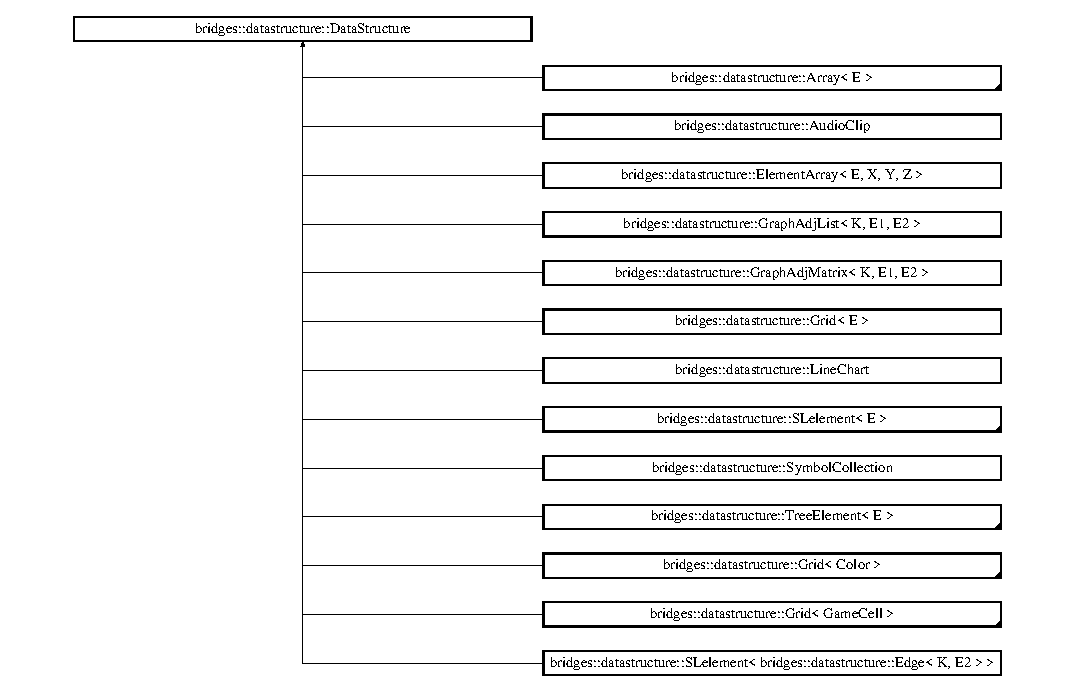
\includegraphics[height=8.216704cm]{classbridges_1_1datastructure_1_1_data_structure}
\end{center}
\end{figure}


\subsection{Detailed Description}
This is the superclass of all data structure types in B\+R\+I\+D\+G\+ES. 

This is the superclass of all data structure types in B\+R\+I\+D\+G\+ES.

All types of B\+R\+I\+D\+G\+ES Elements, \hyperlink{classbridges_1_1datastructure_1_1_array}{Array} and Graphs inherit from this class.

\begin{DoxyDate}{Date}
6/11/15 7/10/16 
\end{DoxyDate}
\begin{DoxyAuthor}{Author}
Dakota Carmer, Kalpathi Subramanian 
\end{DoxyAuthor}
\subsection*{Public Member Functions}
\begin{DoxyCompactItemize}
\item 
virtual \hyperlink{classbridges_1_1datastructure_1_1_data_structure_a54bde1c8f14ca3bff47910a2e48d586a}{$\sim$\+Data\+Structure} ()=default
\item 
virtual const string \hyperlink{classbridges_1_1datastructure_1_1_data_structure_a4ff66cb34409f11fe9fc647f6d8a22ce}{get\+D\+Stype} () const =0
\end{DoxyCompactItemize}
\subsection*{Friends}
\begin{DoxyCompactItemize}
\item 
class \hyperlink{classbridges_1_1datastructure_1_1_data_structure_a5c4164a6c5cd1eab3f12871efc2dbe26}{bridges\+::\+Bridges}
\end{DoxyCompactItemize}


\subsection{Constructor \& Destructor Documentation}
\mbox{\Hypertarget{classbridges_1_1datastructure_1_1_data_structure_a54bde1c8f14ca3bff47910a2e48d586a}\label{classbridges_1_1datastructure_1_1_data_structure_a54bde1c8f14ca3bff47910a2e48d586a}} 
\index{bridges\+::datastructure\+::\+Data\+Structure@{bridges\+::datastructure\+::\+Data\+Structure}!````~Data\+Structure@{$\sim$\+Data\+Structure}}
\index{````~Data\+Structure@{$\sim$\+Data\+Structure}!bridges\+::datastructure\+::\+Data\+Structure@{bridges\+::datastructure\+::\+Data\+Structure}}
\subsubsection{\texorpdfstring{$\sim$\+Data\+Structure()}{~DataStructure()}}
{\footnotesize\ttfamily virtual bridges\+::datastructure\+::\+Data\+Structure\+::$\sim$\+Data\+Structure (\begin{DoxyParamCaption}{ }\end{DoxyParamCaption})\hspace{0.3cm}{\ttfamily [virtual]}, {\ttfamily [default]}}

Virtual Destructor 

\subsection{Member Function Documentation}
\mbox{\Hypertarget{classbridges_1_1datastructure_1_1_data_structure_a4ff66cb34409f11fe9fc647f6d8a22ce}\label{classbridges_1_1datastructure_1_1_data_structure_a4ff66cb34409f11fe9fc647f6d8a22ce}} 
\index{bridges\+::datastructure\+::\+Data\+Structure@{bridges\+::datastructure\+::\+Data\+Structure}!get\+D\+Stype@{get\+D\+Stype}}
\index{get\+D\+Stype@{get\+D\+Stype}!bridges\+::datastructure\+::\+Data\+Structure@{bridges\+::datastructure\+::\+Data\+Structure}}
\subsubsection{\texorpdfstring{get\+D\+Stype()}{getDStype()}}
{\footnotesize\ttfamily virtual const string bridges\+::datastructure\+::\+Data\+Structure\+::get\+D\+Stype (\begin{DoxyParamCaption}{ }\end{DoxyParamCaption}) const\hspace{0.3cm}{\ttfamily [pure virtual]}}

\begin{DoxyReturn}{Returns}
The string representation of this data structure type 
\end{DoxyReturn}


Implemented in \hyperlink{classbridges_1_1game_1_1_game_grid_a07da19700a077e3d0f2cde2cade2ba60}{bridges\+::game\+::\+Game\+Grid}, \hyperlink{classbridges_1_1datastructure_1_1_m_lelement_a735c3cb43648b4d4e7d3316cdc1a1952}{bridges\+::datastructure\+::\+M\+Lelement$<$ E $>$}, \hyperlink{classbridges_1_1datastructure_1_1_array_a3b6d694fe5d336a0a15951d522852e51}{bridges\+::datastructure\+::\+Array$<$ E $>$}, \hyperlink{classbridges_1_1datastructure_1_1_graph_adj_list_adf1bfde5ec7192f3ee334695059f8fa6}{bridges\+::datastructure\+::\+Graph\+Adj\+List$<$ K, E1, E2 $>$}, \hyperlink{classbridges_1_1datastructure_1_1_circ_d_lelement_aec7f9b9dc6626c1a872feb91cd65425d}{bridges\+::datastructure\+::\+Circ\+D\+Lelement$<$ E $>$}, \hyperlink{classbridges_1_1datastructure_1_1_circ_s_lelement_a775ba08a7811fe91c396cb27ba9343ab}{bridges\+::datastructure\+::\+Circ\+S\+Lelement$<$ E $>$}, \hyperlink{classbridges_1_1datastructure_1_1_kd_tree_element_a76f6d9bfadfdec09d0a8564aa0e33235}{bridges\+::datastructure\+::\+Kd\+Tree\+Element$<$ K, E $>$}, \hyperlink{classbridges_1_1datastructure_1_1_line_chart_a431e49c31cdd5f46e978742776306dfa}{bridges\+::datastructure\+::\+Line\+Chart}, \hyperlink{classbridges_1_1datastructure_1_1_grid_a16aeae38446b96f440dea15f2b19334d}{bridges\+::datastructure\+::\+Grid$<$ E $>$}, \hyperlink{classbridges_1_1datastructure_1_1_grid_a16aeae38446b96f440dea15f2b19334d}{bridges\+::datastructure\+::\+Grid$<$ Color $>$}, \hyperlink{classbridges_1_1datastructure_1_1_grid_a16aeae38446b96f440dea15f2b19334d}{bridges\+::datastructure\+::\+Grid$<$ Game\+Cell $>$}, \hyperlink{classbridges_1_1datastructure_1_1_b_s_t_element_a2bb8cc9ec4b6bc5b89ecef0f17be366f}{bridges\+::datastructure\+::\+B\+S\+T\+Element$<$ K, E $>$}, \hyperlink{classbridges_1_1datastructure_1_1_symbol_collection_a8f63c31a48a12127978967b706fc38f5}{bridges\+::datastructure\+::\+Symbol\+Collection}, \hyperlink{classbridges_1_1datastructure_1_1_d_lelement_a736ba8e6901608fb0ab04d781d2cceee}{bridges\+::datastructure\+::\+D\+Lelement$<$ E $>$}, \hyperlink{classbridges_1_1datastructure_1_1_s_lelement_a602156aacacd73d1faa365d68d8af31b}{bridges\+::datastructure\+::\+S\+Lelement$<$ E $>$}, \hyperlink{classbridges_1_1datastructure_1_1_s_lelement_a602156aacacd73d1faa365d68d8af31b}{bridges\+::datastructure\+::\+S\+Lelement$<$ bridges\+::datastructure\+::\+Edge$<$ K, E2 $>$ $>$}, \hyperlink{classbridges_1_1datastructure_1_1_bin_tree_element_aef86e3663785972251547e409fdc757b}{bridges\+::datastructure\+::\+Bin\+Tree\+Element$<$ E $>$}, \hyperlink{classbridges_1_1datastructure_1_1_b_t_element_a2118b6b74f3fe0fec39e3b258a7dee89}{bridges\+::datastructure\+::\+B\+T\+Element$<$ E $>$}, \hyperlink{classbridges_1_1datastructure_1_1_graph_adj_matrix_a2f8c67da1078354156fc646097152c6d}{bridges\+::datastructure\+::\+Graph\+Adj\+Matrix$<$ K, E1, E2 $>$}, \hyperlink{classbridges_1_1datastructure_1_1_a_v_l_tree_element_ab04d1e9ad4630e408041e8137dc9854a}{bridges\+::datastructure\+::\+A\+V\+L\+Tree\+Element$<$ K, E $>$}, \hyperlink{classbridges_1_1datastructure_1_1_color_grid_afad945d648b427ca183a1dface8249b7}{bridges\+::datastructure\+::\+Color\+Grid}, \hyperlink{classbridges_1_1datastructure_1_1_tree_element_a897f34ea284da45e1dc869c3e3b6c9a4}{bridges\+::datastructure\+::\+Tree\+Element$<$ E $>$}, and \hyperlink{classbridges_1_1datastructure_1_1_element_array_a22d8c37e88616105cdb7c755f99fdb20}{bridges\+::datastructure\+::\+Element\+Array$<$ E, X, Y, Z $>$}.



\subsection{Friends And Related Function Documentation}
\mbox{\Hypertarget{classbridges_1_1datastructure_1_1_data_structure_a5c4164a6c5cd1eab3f12871efc2dbe26}\label{classbridges_1_1datastructure_1_1_data_structure_a5c4164a6c5cd1eab3f12871efc2dbe26}} 
\index{bridges\+::datastructure\+::\+Data\+Structure@{bridges\+::datastructure\+::\+Data\+Structure}!bridges\+::\+Bridges@{bridges\+::\+Bridges}}
\index{bridges\+::\+Bridges@{bridges\+::\+Bridges}!bridges\+::datastructure\+::\+Data\+Structure@{bridges\+::datastructure\+::\+Data\+Structure}}
\subsubsection{\texorpdfstring{bridges\+::\+Bridges}{bridges::Bridges}}
{\footnotesize\ttfamily friend class \hyperlink{classbridges_1_1_bridges}{bridges\+::\+Bridges}\hspace{0.3cm}{\ttfamily [friend]}}



The documentation for this class was generated from the following file\+:\begin{DoxyCompactItemize}
\item 
/home/erik/work/bridges/bridges-\/cxx/src/\hyperlink{_data_structure_8h}{Data\+Structure.\+h}\end{DoxyCompactItemize}

\hypertarget{classbridges_1_1datastructure_1_1_d_lelement}{}\section{bridges\+:\+:datastructure\+:\+:D\+Lelement$<$ E $>$ Class Template Reference}
\label{classbridges_1_1datastructure_1_1_d_lelement}\index{bridges\+::datastructure\+::\+D\+Lelement$<$ E $>$@{bridges\+::datastructure\+::\+D\+Lelement$<$ E $>$}}


{\ttfamily \#include $<$D\+Lelement.\+h$>$}

Inheritance diagram for bridges\+:\+:datastructure\+:\+:D\+Lelement$<$ E $>$\+:\begin{figure}[H]
\begin{center}
\leavevmode
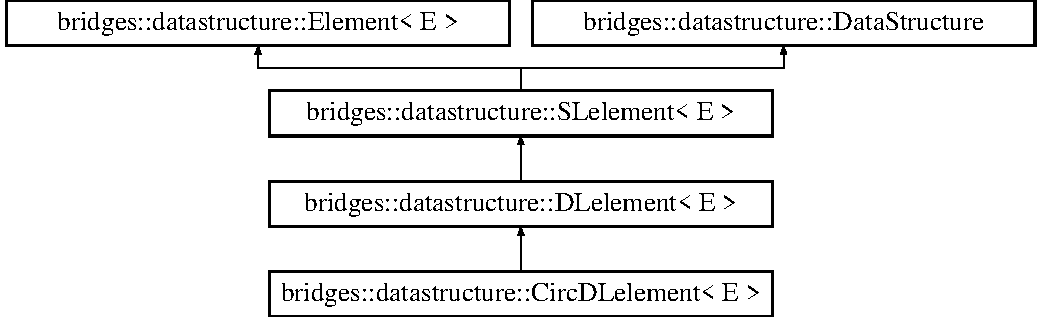
\includegraphics[height=4.000000cm]{classbridges_1_1datastructure_1_1_d_lelement}
\end{center}
\end{figure}


\subsection{Detailed Description}
\subsubsection*{template$<$typename E$>$\newline
class bridges\+::datastructure\+::\+D\+Lelement$<$ E $>$}

The doubly linked list element, derived from \hyperlink{classbridges_1_1datastructure_1_1_s_lelement}{S\+Lelement}. 

This class extends the S\+Lelelement class by adding a previous \hyperlink{classbridges_1_1datastructure_1_1_d_lelement}{D\+Lelement} pointer

There is a tutorial about Doubly Linked Lists \+: \href{http://bridgesuncc.github.io/tutorials/DoublyLinkedList.html}{\tt http\+://bridgesuncc.\+github.\+io/tutorials/\+Doubly\+Linked\+List.\+html}


\begin{DoxyParams}{Parameters}
{\em E} & the application data type\\
\hline
\end{DoxyParams}
\begin{DoxyAuthor}{Author}
Kalpathi Subramanian 
\end{DoxyAuthor}
\begin{DoxyDate}{Date}
6/11/15, 7/12/19 
\end{DoxyDate}
\subsection*{Classes}
\begin{DoxyCompactItemize}
\item 
class \hyperlink{classbridges_1_1datastructure_1_1_d_lelement_1_1_d_lelement__constlisthelper}{D\+Lelement\+\_\+constlisthelper}
\begin{DoxyCompactList}\small\item\em these are helper classes for \hyperlink{classbridges_1_1datastructure_1_1_d_lelement}{D\+Lelement} for easy iteration in a range for loop. It is not meant to be created by the bridges user. But it may be returned by \hyperlink{classbridges_1_1_bridges}{Bridges} to provide an S\+TL compliant list A\+PI. \end{DoxyCompactList}\item 
class \hyperlink{classbridges_1_1datastructure_1_1_d_lelement_1_1_d_lelement__listhelper}{D\+Lelement\+\_\+listhelper}
\begin{DoxyCompactList}\small\item\em these are helper classes for \hyperlink{classbridges_1_1datastructure_1_1_d_lelement}{D\+Lelement} for easy iteration in a range for loop. It is not meant to be created by the bridges user. But it may be returned by \hyperlink{classbridges_1_1_bridges}{Bridges} to provide an S\+TL compliant list A\+PI. \end{DoxyCompactList}\end{DoxyCompactItemize}
\subsection*{Public Member Functions}
\begin{DoxyCompactItemize}
\item 
\hyperlink{classbridges_1_1datastructure_1_1_d_lelement_a7384d570c355bb4762c98b79d4c1e988}{D\+Lelement} (\hyperlink{classbridges_1_1datastructure_1_1_d_lelement}{D\+Lelement} $\ast$n, \hyperlink{classbridges_1_1datastructure_1_1_d_lelement}{D\+Lelement} $\ast$p=nullptr, const E \&val=E(), const string \&lab=string())
\item 
\hyperlink{classbridges_1_1datastructure_1_1_d_lelement_af9c0dc9b417de0466a47be904cd845f6}{D\+Lelement} (const E \&val=E(), const string \&lab=string())
\item 
virtual const string \hyperlink{classbridges_1_1datastructure_1_1_d_lelement_a736ba8e6901608fb0ab04d781d2cceee}{get\+D\+Stype} () const override
\item 
virtual \hyperlink{classbridges_1_1datastructure_1_1_d_lelement}{D\+Lelement} $\ast$ \hyperlink{classbridges_1_1datastructure_1_1_d_lelement_a63212051ea77d74bd751dea00288d2be}{get\+Next} () override
\item 
virtual const \hyperlink{classbridges_1_1datastructure_1_1_d_lelement}{D\+Lelement} $\ast$ \hyperlink{classbridges_1_1datastructure_1_1_d_lelement_a8599e5be5fc1771d4e8a40f6de67b4a7}{get\+Next} () const override
\item 
void \hyperlink{classbridges_1_1datastructure_1_1_d_lelement_ab0fe212dd0e3795b8f3f7978c6bdf805}{set\+Next} (\hyperlink{classbridges_1_1datastructure_1_1_d_lelement}{D\+Lelement} $\ast$n)
\item 
virtual \hyperlink{classbridges_1_1datastructure_1_1_d_lelement}{D\+Lelement} $\ast$ \hyperlink{classbridges_1_1datastructure_1_1_d_lelement_a0edfa823d0fc6f3dba58f85dbf5a11ff}{get\+Prev} ()
\item 
virtual const \hyperlink{classbridges_1_1datastructure_1_1_d_lelement}{D\+Lelement} $\ast$ \hyperlink{classbridges_1_1datastructure_1_1_d_lelement_a66917ba9a9270b8f6b5e4ff258bf3e70}{get\+Prev} () const
\item 
virtual void \hyperlink{classbridges_1_1datastructure_1_1_d_lelement_a748d1ad511509996d8268e75d6ecfeae}{set\+Prev} (\hyperlink{classbridges_1_1datastructure_1_1_d_lelement}{D\+Lelement} $\ast$p)
\end{DoxyCompactItemize}
\subsection*{Additional Inherited Members}


\subsection{Constructor \& Destructor Documentation}
\mbox{\Hypertarget{classbridges_1_1datastructure_1_1_d_lelement_a7384d570c355bb4762c98b79d4c1e988}\label{classbridges_1_1datastructure_1_1_d_lelement_a7384d570c355bb4762c98b79d4c1e988}} 
\index{bridges\+::datastructure\+::\+D\+Lelement@{bridges\+::datastructure\+::\+D\+Lelement}!D\+Lelement@{D\+Lelement}}
\index{D\+Lelement@{D\+Lelement}!bridges\+::datastructure\+::\+D\+Lelement@{bridges\+::datastructure\+::\+D\+Lelement}}
\subsubsection{\texorpdfstring{D\+Lelement()}{DLelement()}\hspace{0.1cm}{\footnotesize\ttfamily [1/2]}}
{\footnotesize\ttfamily template$<$typename E$>$ \\
\hyperlink{classbridges_1_1datastructure_1_1_d_lelement}{bridges\+::datastructure\+::\+D\+Lelement}$<$ E $>$\+::\hyperlink{classbridges_1_1datastructure_1_1_d_lelement}{D\+Lelement} (\begin{DoxyParamCaption}\item[{\hyperlink{classbridges_1_1datastructure_1_1_d_lelement}{D\+Lelement}$<$ E $>$ $\ast$}]{n,  }\item[{\hyperlink{classbridges_1_1datastructure_1_1_d_lelement}{D\+Lelement}$<$ E $>$ $\ast$}]{p = {\ttfamily nullptr},  }\item[{const E \&}]{val = {\ttfamily E()},  }\item[{const string \&}]{lab = {\ttfamily string()} }\end{DoxyParamCaption})\hspace{0.3cm}{\ttfamily [inline]}}

Constructs a dlelement with the provided value, label, next and previous elements. The defaults will be used if not provided.


\begin{DoxyParams}{Parameters}
{\em n} & The next \hyperlink{classbridges_1_1datastructure_1_1_d_lelement}{D\+Lelement} \\
\hline
{\em p} & The previous \hyperlink{classbridges_1_1datastructure_1_1_d_lelement}{D\+Lelement} \\
\hline
{\em val} & The data to hold \\
\hline
{\em lab} & The label to show \\
\hline
\end{DoxyParams}
\mbox{\Hypertarget{classbridges_1_1datastructure_1_1_d_lelement_af9c0dc9b417de0466a47be904cd845f6}\label{classbridges_1_1datastructure_1_1_d_lelement_af9c0dc9b417de0466a47be904cd845f6}} 
\index{bridges\+::datastructure\+::\+D\+Lelement@{bridges\+::datastructure\+::\+D\+Lelement}!D\+Lelement@{D\+Lelement}}
\index{D\+Lelement@{D\+Lelement}!bridges\+::datastructure\+::\+D\+Lelement@{bridges\+::datastructure\+::\+D\+Lelement}}
\subsubsection{\texorpdfstring{D\+Lelement()}{DLelement()}\hspace{0.1cm}{\footnotesize\ttfamily [2/2]}}
{\footnotesize\ttfamily template$<$typename E$>$ \\
\hyperlink{classbridges_1_1datastructure_1_1_d_lelement}{bridges\+::datastructure\+::\+D\+Lelement}$<$ E $>$\+::\hyperlink{classbridges_1_1datastructure_1_1_d_lelement}{D\+Lelement} (\begin{DoxyParamCaption}\item[{const E \&}]{val = {\ttfamily E()},  }\item[{const string \&}]{lab = {\ttfamily string()} }\end{DoxyParamCaption})\hspace{0.3cm}{\ttfamily [inline]}}

Constructs a dlelement with the provided value and label, setting the next and previous dlelements to N\+U\+LL. The defaults will be used if not provided.


\begin{DoxyParams}{Parameters}
{\em val} & The data to hold \\
\hline
{\em lab} & The label to show \\
\hline
\end{DoxyParams}


\subsection{Member Function Documentation}
\mbox{\Hypertarget{classbridges_1_1datastructure_1_1_d_lelement_a736ba8e6901608fb0ab04d781d2cceee}\label{classbridges_1_1datastructure_1_1_d_lelement_a736ba8e6901608fb0ab04d781d2cceee}} 
\index{bridges\+::datastructure\+::\+D\+Lelement@{bridges\+::datastructure\+::\+D\+Lelement}!get\+D\+Stype@{get\+D\+Stype}}
\index{get\+D\+Stype@{get\+D\+Stype}!bridges\+::datastructure\+::\+D\+Lelement@{bridges\+::datastructure\+::\+D\+Lelement}}
\subsubsection{\texorpdfstring{get\+D\+Stype()}{getDStype()}}
{\footnotesize\ttfamily template$<$typename E$>$ \\
virtual const string \hyperlink{classbridges_1_1datastructure_1_1_d_lelement}{bridges\+::datastructure\+::\+D\+Lelement}$<$ E $>$\+::get\+D\+Stype (\begin{DoxyParamCaption}{ }\end{DoxyParamCaption}) const\hspace{0.3cm}{\ttfamily [inline]}, {\ttfamily [override]}, {\ttfamily [virtual]}}

Return the data structure type

\begin{DoxyReturn}{Returns}
The name of this data structure type 
\end{DoxyReturn}


Reimplemented from \hyperlink{classbridges_1_1datastructure_1_1_s_lelement_a602156aacacd73d1faa365d68d8af31b}{bridges\+::datastructure\+::\+S\+Lelement$<$ E $>$}.



Reimplemented in \hyperlink{classbridges_1_1datastructure_1_1_circ_d_lelement_aec7f9b9dc6626c1a872feb91cd65425d}{bridges\+::datastructure\+::\+Circ\+D\+Lelement$<$ E $>$}.

\mbox{\Hypertarget{classbridges_1_1datastructure_1_1_d_lelement_a63212051ea77d74bd751dea00288d2be}\label{classbridges_1_1datastructure_1_1_d_lelement_a63212051ea77d74bd751dea00288d2be}} 
\index{bridges\+::datastructure\+::\+D\+Lelement@{bridges\+::datastructure\+::\+D\+Lelement}!get\+Next@{get\+Next}}
\index{get\+Next@{get\+Next}!bridges\+::datastructure\+::\+D\+Lelement@{bridges\+::datastructure\+::\+D\+Lelement}}
\subsubsection{\texorpdfstring{get\+Next()}{getNext()}\hspace{0.1cm}{\footnotesize\ttfamily [1/2]}}
{\footnotesize\ttfamily template$<$typename E$>$ \\
virtual \hyperlink{classbridges_1_1datastructure_1_1_d_lelement}{D\+Lelement}$\ast$ \hyperlink{classbridges_1_1datastructure_1_1_d_lelement}{bridges\+::datastructure\+::\+D\+Lelement}$<$ E $>$\+::get\+Next (\begin{DoxyParamCaption}{ }\end{DoxyParamCaption})\hspace{0.3cm}{\ttfamily [inline]}, {\ttfamily [override]}, {\ttfamily [virtual]}}

Return the next DL element.

\begin{DoxyReturn}{Returns}
The next \hyperlink{classbridges_1_1datastructure_1_1_d_lelement}{D\+Lelement} 
\end{DoxyReturn}


Reimplemented from \hyperlink{classbridges_1_1datastructure_1_1_s_lelement_ae43dd771d9ced7cb17f1d35f34cd9a42}{bridges\+::datastructure\+::\+S\+Lelement$<$ E $>$}.



Reimplemented in \hyperlink{classbridges_1_1datastructure_1_1_circ_d_lelement_a80681d0382643a6df21da1bec4067004}{bridges\+::datastructure\+::\+Circ\+D\+Lelement$<$ E $>$}.

\mbox{\Hypertarget{classbridges_1_1datastructure_1_1_d_lelement_a8599e5be5fc1771d4e8a40f6de67b4a7}\label{classbridges_1_1datastructure_1_1_d_lelement_a8599e5be5fc1771d4e8a40f6de67b4a7}} 
\index{bridges\+::datastructure\+::\+D\+Lelement@{bridges\+::datastructure\+::\+D\+Lelement}!get\+Next@{get\+Next}}
\index{get\+Next@{get\+Next}!bridges\+::datastructure\+::\+D\+Lelement@{bridges\+::datastructure\+::\+D\+Lelement}}
\subsubsection{\texorpdfstring{get\+Next()}{getNext()}\hspace{0.1cm}{\footnotesize\ttfamily [2/2]}}
{\footnotesize\ttfamily template$<$typename E$>$ \\
virtual const \hyperlink{classbridges_1_1datastructure_1_1_d_lelement}{D\+Lelement}$\ast$ \hyperlink{classbridges_1_1datastructure_1_1_d_lelement}{bridges\+::datastructure\+::\+D\+Lelement}$<$ E $>$\+::get\+Next (\begin{DoxyParamCaption}{ }\end{DoxyParamCaption}) const\hspace{0.3cm}{\ttfamily [inline]}, {\ttfamily [override]}, {\ttfamily [virtual]}}

Constant version

\begin{DoxyReturn}{Returns}
The next \hyperlink{classbridges_1_1datastructure_1_1_d_lelement}{D\+Lelement} 
\end{DoxyReturn}


Reimplemented from \hyperlink{classbridges_1_1datastructure_1_1_s_lelement_a8c62cb82fa64bbfe9ebb7334a5fea417}{bridges\+::datastructure\+::\+S\+Lelement$<$ E $>$}.



Reimplemented in \hyperlink{classbridges_1_1datastructure_1_1_circ_d_lelement_a3b54f07ffa49151ed13d8b8df964a4ee}{bridges\+::datastructure\+::\+Circ\+D\+Lelement$<$ E $>$}.

\mbox{\Hypertarget{classbridges_1_1datastructure_1_1_d_lelement_a0edfa823d0fc6f3dba58f85dbf5a11ff}\label{classbridges_1_1datastructure_1_1_d_lelement_a0edfa823d0fc6f3dba58f85dbf5a11ff}} 
\index{bridges\+::datastructure\+::\+D\+Lelement@{bridges\+::datastructure\+::\+D\+Lelement}!get\+Prev@{get\+Prev}}
\index{get\+Prev@{get\+Prev}!bridges\+::datastructure\+::\+D\+Lelement@{bridges\+::datastructure\+::\+D\+Lelement}}
\subsubsection{\texorpdfstring{get\+Prev()}{getPrev()}\hspace{0.1cm}{\footnotesize\ttfamily [1/2]}}
{\footnotesize\ttfamily template$<$typename E$>$ \\
virtual \hyperlink{classbridges_1_1datastructure_1_1_d_lelement}{D\+Lelement}$\ast$ \hyperlink{classbridges_1_1datastructure_1_1_d_lelement}{bridges\+::datastructure\+::\+D\+Lelement}$<$ E $>$\+::get\+Prev (\begin{DoxyParamCaption}{ }\end{DoxyParamCaption})\hspace{0.3cm}{\ttfamily [inline]}, {\ttfamily [virtual]}}

Returns the previous element in the list \begin{DoxyReturn}{Returns}
The previous \hyperlink{classbridges_1_1datastructure_1_1_d_lelement}{D\+Lelement} 
\end{DoxyReturn}


Reimplemented in \hyperlink{classbridges_1_1datastructure_1_1_circ_d_lelement_a5218bb590a588e1d1aaa8f53403ed0cb}{bridges\+::datastructure\+::\+Circ\+D\+Lelement$<$ E $>$}.

\mbox{\Hypertarget{classbridges_1_1datastructure_1_1_d_lelement_a66917ba9a9270b8f6b5e4ff258bf3e70}\label{classbridges_1_1datastructure_1_1_d_lelement_a66917ba9a9270b8f6b5e4ff258bf3e70}} 
\index{bridges\+::datastructure\+::\+D\+Lelement@{bridges\+::datastructure\+::\+D\+Lelement}!get\+Prev@{get\+Prev}}
\index{get\+Prev@{get\+Prev}!bridges\+::datastructure\+::\+D\+Lelement@{bridges\+::datastructure\+::\+D\+Lelement}}
\subsubsection{\texorpdfstring{get\+Prev()}{getPrev()}\hspace{0.1cm}{\footnotesize\ttfamily [2/2]}}
{\footnotesize\ttfamily template$<$typename E$>$ \\
virtual const \hyperlink{classbridges_1_1datastructure_1_1_d_lelement}{D\+Lelement}$\ast$ \hyperlink{classbridges_1_1datastructure_1_1_d_lelement}{bridges\+::datastructure\+::\+D\+Lelement}$<$ E $>$\+::get\+Prev (\begin{DoxyParamCaption}{ }\end{DoxyParamCaption}) const\hspace{0.3cm}{\ttfamily [inline]}, {\ttfamily [virtual]}}

Returns the previous element -\/ Constant version

\begin{DoxyReturn}{Returns}
The previous \hyperlink{classbridges_1_1datastructure_1_1_d_lelement}{D\+Lelement} 
\end{DoxyReturn}


Reimplemented in \hyperlink{classbridges_1_1datastructure_1_1_circ_d_lelement_a80a08e1d066b1a1f474aa9fd3bc29972}{bridges\+::datastructure\+::\+Circ\+D\+Lelement$<$ E $>$}.

\mbox{\Hypertarget{classbridges_1_1datastructure_1_1_d_lelement_ab0fe212dd0e3795b8f3f7978c6bdf805}\label{classbridges_1_1datastructure_1_1_d_lelement_ab0fe212dd0e3795b8f3f7978c6bdf805}} 
\index{bridges\+::datastructure\+::\+D\+Lelement@{bridges\+::datastructure\+::\+D\+Lelement}!set\+Next@{set\+Next}}
\index{set\+Next@{set\+Next}!bridges\+::datastructure\+::\+D\+Lelement@{bridges\+::datastructure\+::\+D\+Lelement}}
\subsubsection{\texorpdfstring{set\+Next()}{setNext()}}
{\footnotesize\ttfamily template$<$typename E$>$ \\
void \hyperlink{classbridges_1_1datastructure_1_1_d_lelement}{bridges\+::datastructure\+::\+D\+Lelement}$<$ E $>$\+::set\+Next (\begin{DoxyParamCaption}\item[{\hyperlink{classbridges_1_1datastructure_1_1_d_lelement}{D\+Lelement}$<$ E $>$ $\ast$}]{n }\end{DoxyParamCaption})\hspace{0.3cm}{\ttfamily [inline]}}

Sets next element to \char`\"{}n\char`\"{}


\begin{DoxyParams}{Parameters}
{\em n} & The next \hyperlink{classbridges_1_1datastructure_1_1_d_lelement}{D\+Lelement} \\
\hline
\end{DoxyParams}
\mbox{\Hypertarget{classbridges_1_1datastructure_1_1_d_lelement_a748d1ad511509996d8268e75d6ecfeae}\label{classbridges_1_1datastructure_1_1_d_lelement_a748d1ad511509996d8268e75d6ecfeae}} 
\index{bridges\+::datastructure\+::\+D\+Lelement@{bridges\+::datastructure\+::\+D\+Lelement}!set\+Prev@{set\+Prev}}
\index{set\+Prev@{set\+Prev}!bridges\+::datastructure\+::\+D\+Lelement@{bridges\+::datastructure\+::\+D\+Lelement}}
\subsubsection{\texorpdfstring{set\+Prev()}{setPrev()}}
{\footnotesize\ttfamily template$<$typename E$>$ \\
virtual void \hyperlink{classbridges_1_1datastructure_1_1_d_lelement}{bridges\+::datastructure\+::\+D\+Lelement}$<$ E $>$\+::set\+Prev (\begin{DoxyParamCaption}\item[{\hyperlink{classbridges_1_1datastructure_1_1_d_lelement}{D\+Lelement}$<$ E $>$ $\ast$}]{p }\end{DoxyParamCaption})\hspace{0.3cm}{\ttfamily [inline]}, {\ttfamily [virtual]}}

Sets prev element to \char`\"{}p\char`\"{}


\begin{DoxyParams}{Parameters}
{\em p} & The previous element \\
\hline
\end{DoxyParams}


The documentation for this class was generated from the following file\+:\begin{DoxyCompactItemize}
\item 
/home/erik/work/bridges/bridges-\/cxx/src/\hyperlink{_d_lelement_8h}{D\+Lelement.\+h}\end{DoxyCompactItemize}

\hypertarget{classbridges_1_1datastructure_1_1_d_lelement_1_1_d_lelement__constlisthelper}{}\section{bridges\+:\+:datastructure\+:\+:D\+Lelement$<$ E $>$\+:\+:D\+Lelement\+\_\+constlisthelper Class Reference}
\label{classbridges_1_1datastructure_1_1_d_lelement_1_1_d_lelement__constlisthelper}\index{bridges\+::datastructure\+::\+D\+Lelement$<$ E $>$\+::\+D\+Lelement\+\_\+constlisthelper@{bridges\+::datastructure\+::\+D\+Lelement$<$ E $>$\+::\+D\+Lelement\+\_\+constlisthelper}}


{\ttfamily \#include $<$D\+Lelement.\+h$>$}



\subsection{Detailed Description}
\subsubsection*{template$<$typename E$>$\newline
class bridges\+::datastructure\+::\+D\+Lelement$<$ E $>$\+::\+D\+Lelement\+\_\+constlisthelper}

these are helper classes for \hyperlink{classbridges_1_1datastructure_1_1_d_lelement}{D\+Lelement} for easy iteration in a range for loop. It is not meant to be created by the bridges user. But it may be returned by \hyperlink{classbridges_1_1_bridges}{Bridges} to provide an S\+TL compliant list A\+PI. \subsection*{Classes}
\begin{DoxyCompactItemize}
\item 
class \hyperlink{classbridges_1_1datastructure_1_1_d_lelement_1_1_d_lelement__constlisthelper_1_1iterator}{iterator}
\end{DoxyCompactItemize}
\subsection*{Public Member Functions}
\begin{DoxyCompactItemize}
\item 
\hyperlink{classbridges_1_1datastructure_1_1_d_lelement_1_1_d_lelement__constlisthelper_a2c05f3f43826108552aa8bd325b48753}{D\+Lelement\+\_\+constlisthelper} (typename \hyperlink{classbridges_1_1datastructure_1_1_d_lelement}{bridges\+::datastructure\+::\+D\+Lelement}$<$ E $>$ const $\ast$s)
\item 
\hyperlink{classbridges_1_1datastructure_1_1_d_lelement_1_1_d_lelement__constlisthelper_1_1iterator}{iterator} \hyperlink{classbridges_1_1datastructure_1_1_d_lelement_1_1_d_lelement__constlisthelper_a84507b186afcf37d5c11c341f37b74de}{begin} ()
\item 
\hyperlink{classbridges_1_1datastructure_1_1_d_lelement_1_1_d_lelement__constlisthelper_1_1iterator}{iterator} \hyperlink{classbridges_1_1datastructure_1_1_d_lelement_1_1_d_lelement__constlisthelper_a3caced1b593034beee0fa105e1f7a663}{end} ()
\item 
\hyperlink{classbridges_1_1datastructure_1_1_d_lelement_1_1_d_lelement__constlisthelper_1_1iterator}{iterator} \hyperlink{classbridges_1_1datastructure_1_1_d_lelement_1_1_d_lelement__constlisthelper_a81828d8ccd860b62812dd4b824df1a06}{rbegin} ()
\item 
\hyperlink{classbridges_1_1datastructure_1_1_d_lelement_1_1_d_lelement__constlisthelper_1_1iterator}{iterator} \hyperlink{classbridges_1_1datastructure_1_1_d_lelement_1_1_d_lelement__constlisthelper_a1085a069b94d7d78f81de9764e4db6b4}{rend} ()
\end{DoxyCompactItemize}


\subsection{Constructor \& Destructor Documentation}
\mbox{\Hypertarget{classbridges_1_1datastructure_1_1_d_lelement_1_1_d_lelement__constlisthelper_a2c05f3f43826108552aa8bd325b48753}\label{classbridges_1_1datastructure_1_1_d_lelement_1_1_d_lelement__constlisthelper_a2c05f3f43826108552aa8bd325b48753}} 
\index{bridges\+::datastructure\+::\+D\+Lelement\+::\+D\+Lelement\+\_\+constlisthelper@{bridges\+::datastructure\+::\+D\+Lelement\+::\+D\+Lelement\+\_\+constlisthelper}!D\+Lelement\+\_\+constlisthelper@{D\+Lelement\+\_\+constlisthelper}}
\index{D\+Lelement\+\_\+constlisthelper@{D\+Lelement\+\_\+constlisthelper}!bridges\+::datastructure\+::\+D\+Lelement\+::\+D\+Lelement\+\_\+constlisthelper@{bridges\+::datastructure\+::\+D\+Lelement\+::\+D\+Lelement\+\_\+constlisthelper}}
\subsubsection{\texorpdfstring{D\+Lelement\+\_\+constlisthelper()}{DLelement\_constlisthelper()}}
{\footnotesize\ttfamily template$<$typename E$>$ \\
\hyperlink{classbridges_1_1datastructure_1_1_d_lelement}{bridges\+::datastructure\+::\+D\+Lelement}$<$ E $>$\+::D\+Lelement\+\_\+constlisthelper\+::\+D\+Lelement\+\_\+constlisthelper (\begin{DoxyParamCaption}\item[{typename \hyperlink{classbridges_1_1datastructure_1_1_d_lelement}{bridges\+::datastructure\+::\+D\+Lelement}$<$ E $>$ const $\ast$}]{s }\end{DoxyParamCaption})\hspace{0.3cm}{\ttfamily [inline]}}



\subsection{Member Function Documentation}
\mbox{\Hypertarget{classbridges_1_1datastructure_1_1_d_lelement_1_1_d_lelement__constlisthelper_a84507b186afcf37d5c11c341f37b74de}\label{classbridges_1_1datastructure_1_1_d_lelement_1_1_d_lelement__constlisthelper_a84507b186afcf37d5c11c341f37b74de}} 
\index{bridges\+::datastructure\+::\+D\+Lelement\+::\+D\+Lelement\+\_\+constlisthelper@{bridges\+::datastructure\+::\+D\+Lelement\+::\+D\+Lelement\+\_\+constlisthelper}!begin@{begin}}
\index{begin@{begin}!bridges\+::datastructure\+::\+D\+Lelement\+::\+D\+Lelement\+\_\+constlisthelper@{bridges\+::datastructure\+::\+D\+Lelement\+::\+D\+Lelement\+\_\+constlisthelper}}
\subsubsection{\texorpdfstring{begin()}{begin()}}
{\footnotesize\ttfamily template$<$typename E$>$ \\
\hyperlink{classbridges_1_1datastructure_1_1_d_lelement_1_1_d_lelement__constlisthelper_1_1iterator}{iterator} \hyperlink{classbridges_1_1datastructure_1_1_d_lelement}{bridges\+::datastructure\+::\+D\+Lelement}$<$ E $>$\+::D\+Lelement\+\_\+constlisthelper\+::begin (\begin{DoxyParamCaption}{ }\end{DoxyParamCaption})\hspace{0.3cm}{\ttfamily [inline]}}

\mbox{\Hypertarget{classbridges_1_1datastructure_1_1_d_lelement_1_1_d_lelement__constlisthelper_a3caced1b593034beee0fa105e1f7a663}\label{classbridges_1_1datastructure_1_1_d_lelement_1_1_d_lelement__constlisthelper_a3caced1b593034beee0fa105e1f7a663}} 
\index{bridges\+::datastructure\+::\+D\+Lelement\+::\+D\+Lelement\+\_\+constlisthelper@{bridges\+::datastructure\+::\+D\+Lelement\+::\+D\+Lelement\+\_\+constlisthelper}!end@{end}}
\index{end@{end}!bridges\+::datastructure\+::\+D\+Lelement\+::\+D\+Lelement\+\_\+constlisthelper@{bridges\+::datastructure\+::\+D\+Lelement\+::\+D\+Lelement\+\_\+constlisthelper}}
\subsubsection{\texorpdfstring{end()}{end()}}
{\footnotesize\ttfamily template$<$typename E$>$ \\
\hyperlink{classbridges_1_1datastructure_1_1_d_lelement_1_1_d_lelement__constlisthelper_1_1iterator}{iterator} \hyperlink{classbridges_1_1datastructure_1_1_d_lelement}{bridges\+::datastructure\+::\+D\+Lelement}$<$ E $>$\+::D\+Lelement\+\_\+constlisthelper\+::end (\begin{DoxyParamCaption}{ }\end{DoxyParamCaption})\hspace{0.3cm}{\ttfamily [inline]}}

\mbox{\Hypertarget{classbridges_1_1datastructure_1_1_d_lelement_1_1_d_lelement__constlisthelper_a81828d8ccd860b62812dd4b824df1a06}\label{classbridges_1_1datastructure_1_1_d_lelement_1_1_d_lelement__constlisthelper_a81828d8ccd860b62812dd4b824df1a06}} 
\index{bridges\+::datastructure\+::\+D\+Lelement\+::\+D\+Lelement\+\_\+constlisthelper@{bridges\+::datastructure\+::\+D\+Lelement\+::\+D\+Lelement\+\_\+constlisthelper}!rbegin@{rbegin}}
\index{rbegin@{rbegin}!bridges\+::datastructure\+::\+D\+Lelement\+::\+D\+Lelement\+\_\+constlisthelper@{bridges\+::datastructure\+::\+D\+Lelement\+::\+D\+Lelement\+\_\+constlisthelper}}
\subsubsection{\texorpdfstring{rbegin()}{rbegin()}}
{\footnotesize\ttfamily template$<$typename E$>$ \\
\hyperlink{classbridges_1_1datastructure_1_1_d_lelement_1_1_d_lelement__constlisthelper_1_1iterator}{iterator} \hyperlink{classbridges_1_1datastructure_1_1_d_lelement}{bridges\+::datastructure\+::\+D\+Lelement}$<$ E $>$\+::D\+Lelement\+\_\+constlisthelper\+::rbegin (\begin{DoxyParamCaption}{ }\end{DoxyParamCaption})\hspace{0.3cm}{\ttfamily [inline]}}

\mbox{\Hypertarget{classbridges_1_1datastructure_1_1_d_lelement_1_1_d_lelement__constlisthelper_a1085a069b94d7d78f81de9764e4db6b4}\label{classbridges_1_1datastructure_1_1_d_lelement_1_1_d_lelement__constlisthelper_a1085a069b94d7d78f81de9764e4db6b4}} 
\index{bridges\+::datastructure\+::\+D\+Lelement\+::\+D\+Lelement\+\_\+constlisthelper@{bridges\+::datastructure\+::\+D\+Lelement\+::\+D\+Lelement\+\_\+constlisthelper}!rend@{rend}}
\index{rend@{rend}!bridges\+::datastructure\+::\+D\+Lelement\+::\+D\+Lelement\+\_\+constlisthelper@{bridges\+::datastructure\+::\+D\+Lelement\+::\+D\+Lelement\+\_\+constlisthelper}}
\subsubsection{\texorpdfstring{rend()}{rend()}}
{\footnotesize\ttfamily template$<$typename E$>$ \\
\hyperlink{classbridges_1_1datastructure_1_1_d_lelement_1_1_d_lelement__constlisthelper_1_1iterator}{iterator} \hyperlink{classbridges_1_1datastructure_1_1_d_lelement}{bridges\+::datastructure\+::\+D\+Lelement}$<$ E $>$\+::D\+Lelement\+\_\+constlisthelper\+::rend (\begin{DoxyParamCaption}{ }\end{DoxyParamCaption})\hspace{0.3cm}{\ttfamily [inline]}}



The documentation for this class was generated from the following file\+:\begin{DoxyCompactItemize}
\item 
/home/erik/work/bridges/bridges-\/cxx/src/\hyperlink{_d_lelement_8h}{D\+Lelement.\+h}\end{DoxyCompactItemize}

\hypertarget{classbridges_1_1datastructure_1_1_d_lelement_1_1_d_lelement__listhelper}{}\section{bridges\+:\+:datastructure\+:\+:D\+Lelement$<$ E $>$\+:\+:D\+Lelement\+\_\+listhelper Class Reference}
\label{classbridges_1_1datastructure_1_1_d_lelement_1_1_d_lelement__listhelper}\index{bridges\+::datastructure\+::\+D\+Lelement$<$ E $>$\+::\+D\+Lelement\+\_\+listhelper@{bridges\+::datastructure\+::\+D\+Lelement$<$ E $>$\+::\+D\+Lelement\+\_\+listhelper}}


{\ttfamily \#include $<$D\+Lelement.\+h$>$}



\subsection{Detailed Description}
\subsubsection*{template$<$typename E$>$\newline
class bridges\+::datastructure\+::\+D\+Lelement$<$ E $>$\+::\+D\+Lelement\+\_\+listhelper}

these are helper classes for \hyperlink{classbridges_1_1datastructure_1_1_d_lelement}{D\+Lelement} for easy iteration in a range for loop. It is not meant to be created by the bridges user. But it may be returned by \hyperlink{classbridges_1_1_bridges}{Bridges} to provide an S\+TL compliant list A\+PI. \subsection*{Classes}
\begin{DoxyCompactItemize}
\item 
class \hyperlink{classbridges_1_1datastructure_1_1_d_lelement_1_1_d_lelement__listhelper_1_1iterator}{iterator}
\end{DoxyCompactItemize}
\subsection*{Public Member Functions}
\begin{DoxyCompactItemize}
\item 
\hyperlink{classbridges_1_1datastructure_1_1_d_lelement_1_1_d_lelement__listhelper_afa61fdecd0ce37512ffa7bf89e0383cd}{D\+Lelement\+\_\+listhelper} (typename \hyperlink{classbridges_1_1datastructure_1_1_d_lelement}{bridges\+::datastructure\+::\+D\+Lelement}$<$ E $>$ $\ast$s)
\item 
\hyperlink{classbridges_1_1datastructure_1_1_d_lelement_1_1_d_lelement__listhelper_1_1iterator}{iterator} \hyperlink{classbridges_1_1datastructure_1_1_d_lelement_1_1_d_lelement__listhelper_a2739518ed5c02b3f8e97c23a777a0b59}{begin} ()
\item 
\hyperlink{classbridges_1_1datastructure_1_1_d_lelement_1_1_d_lelement__listhelper_1_1iterator}{iterator} \hyperlink{classbridges_1_1datastructure_1_1_d_lelement_1_1_d_lelement__listhelper_a1570c3746046008ce249cb9843a16be6}{end} ()
\item 
\hyperlink{classbridges_1_1datastructure_1_1_d_lelement_1_1_d_lelement__listhelper_1_1iterator}{iterator} \hyperlink{classbridges_1_1datastructure_1_1_d_lelement_1_1_d_lelement__listhelper_aa0e15872d603e1712d1c3fee6d16a630}{rbegin} ()
\item 
\hyperlink{classbridges_1_1datastructure_1_1_d_lelement_1_1_d_lelement__listhelper_1_1iterator}{iterator} \hyperlink{classbridges_1_1datastructure_1_1_d_lelement_1_1_d_lelement__listhelper_aaad384a46635fdb9c4d2e076ed988bb3}{rend} ()
\end{DoxyCompactItemize}


\subsection{Constructor \& Destructor Documentation}
\mbox{\Hypertarget{classbridges_1_1datastructure_1_1_d_lelement_1_1_d_lelement__listhelper_afa61fdecd0ce37512ffa7bf89e0383cd}\label{classbridges_1_1datastructure_1_1_d_lelement_1_1_d_lelement__listhelper_afa61fdecd0ce37512ffa7bf89e0383cd}} 
\index{bridges\+::datastructure\+::\+D\+Lelement\+::\+D\+Lelement\+\_\+listhelper@{bridges\+::datastructure\+::\+D\+Lelement\+::\+D\+Lelement\+\_\+listhelper}!D\+Lelement\+\_\+listhelper@{D\+Lelement\+\_\+listhelper}}
\index{D\+Lelement\+\_\+listhelper@{D\+Lelement\+\_\+listhelper}!bridges\+::datastructure\+::\+D\+Lelement\+::\+D\+Lelement\+\_\+listhelper@{bridges\+::datastructure\+::\+D\+Lelement\+::\+D\+Lelement\+\_\+listhelper}}
\subsubsection{\texorpdfstring{D\+Lelement\+\_\+listhelper()}{DLelement\_listhelper()}}
{\footnotesize\ttfamily template$<$typename E$>$ \\
\hyperlink{classbridges_1_1datastructure_1_1_d_lelement}{bridges\+::datastructure\+::\+D\+Lelement}$<$ E $>$\+::D\+Lelement\+\_\+listhelper\+::\+D\+Lelement\+\_\+listhelper (\begin{DoxyParamCaption}\item[{typename \hyperlink{classbridges_1_1datastructure_1_1_d_lelement}{bridges\+::datastructure\+::\+D\+Lelement}$<$ E $>$ $\ast$}]{s }\end{DoxyParamCaption})\hspace{0.3cm}{\ttfamily [inline]}}



\subsection{Member Function Documentation}
\mbox{\Hypertarget{classbridges_1_1datastructure_1_1_d_lelement_1_1_d_lelement__listhelper_a2739518ed5c02b3f8e97c23a777a0b59}\label{classbridges_1_1datastructure_1_1_d_lelement_1_1_d_lelement__listhelper_a2739518ed5c02b3f8e97c23a777a0b59}} 
\index{bridges\+::datastructure\+::\+D\+Lelement\+::\+D\+Lelement\+\_\+listhelper@{bridges\+::datastructure\+::\+D\+Lelement\+::\+D\+Lelement\+\_\+listhelper}!begin@{begin}}
\index{begin@{begin}!bridges\+::datastructure\+::\+D\+Lelement\+::\+D\+Lelement\+\_\+listhelper@{bridges\+::datastructure\+::\+D\+Lelement\+::\+D\+Lelement\+\_\+listhelper}}
\subsubsection{\texorpdfstring{begin()}{begin()}}
{\footnotesize\ttfamily template$<$typename E$>$ \\
\hyperlink{classbridges_1_1datastructure_1_1_d_lelement_1_1_d_lelement__listhelper_1_1iterator}{iterator} \hyperlink{classbridges_1_1datastructure_1_1_d_lelement}{bridges\+::datastructure\+::\+D\+Lelement}$<$ E $>$\+::D\+Lelement\+\_\+listhelper\+::begin (\begin{DoxyParamCaption}{ }\end{DoxyParamCaption})\hspace{0.3cm}{\ttfamily [inline]}}

\mbox{\Hypertarget{classbridges_1_1datastructure_1_1_d_lelement_1_1_d_lelement__listhelper_a1570c3746046008ce249cb9843a16be6}\label{classbridges_1_1datastructure_1_1_d_lelement_1_1_d_lelement__listhelper_a1570c3746046008ce249cb9843a16be6}} 
\index{bridges\+::datastructure\+::\+D\+Lelement\+::\+D\+Lelement\+\_\+listhelper@{bridges\+::datastructure\+::\+D\+Lelement\+::\+D\+Lelement\+\_\+listhelper}!end@{end}}
\index{end@{end}!bridges\+::datastructure\+::\+D\+Lelement\+::\+D\+Lelement\+\_\+listhelper@{bridges\+::datastructure\+::\+D\+Lelement\+::\+D\+Lelement\+\_\+listhelper}}
\subsubsection{\texorpdfstring{end()}{end()}}
{\footnotesize\ttfamily template$<$typename E$>$ \\
\hyperlink{classbridges_1_1datastructure_1_1_d_lelement_1_1_d_lelement__listhelper_1_1iterator}{iterator} \hyperlink{classbridges_1_1datastructure_1_1_d_lelement}{bridges\+::datastructure\+::\+D\+Lelement}$<$ E $>$\+::D\+Lelement\+\_\+listhelper\+::end (\begin{DoxyParamCaption}{ }\end{DoxyParamCaption})\hspace{0.3cm}{\ttfamily [inline]}}

\mbox{\Hypertarget{classbridges_1_1datastructure_1_1_d_lelement_1_1_d_lelement__listhelper_aa0e15872d603e1712d1c3fee6d16a630}\label{classbridges_1_1datastructure_1_1_d_lelement_1_1_d_lelement__listhelper_aa0e15872d603e1712d1c3fee6d16a630}} 
\index{bridges\+::datastructure\+::\+D\+Lelement\+::\+D\+Lelement\+\_\+listhelper@{bridges\+::datastructure\+::\+D\+Lelement\+::\+D\+Lelement\+\_\+listhelper}!rbegin@{rbegin}}
\index{rbegin@{rbegin}!bridges\+::datastructure\+::\+D\+Lelement\+::\+D\+Lelement\+\_\+listhelper@{bridges\+::datastructure\+::\+D\+Lelement\+::\+D\+Lelement\+\_\+listhelper}}
\subsubsection{\texorpdfstring{rbegin()}{rbegin()}}
{\footnotesize\ttfamily template$<$typename E$>$ \\
\hyperlink{classbridges_1_1datastructure_1_1_d_lelement_1_1_d_lelement__listhelper_1_1iterator}{iterator} \hyperlink{classbridges_1_1datastructure_1_1_d_lelement}{bridges\+::datastructure\+::\+D\+Lelement}$<$ E $>$\+::D\+Lelement\+\_\+listhelper\+::rbegin (\begin{DoxyParamCaption}{ }\end{DoxyParamCaption})\hspace{0.3cm}{\ttfamily [inline]}}

\mbox{\Hypertarget{classbridges_1_1datastructure_1_1_d_lelement_1_1_d_lelement__listhelper_aaad384a46635fdb9c4d2e076ed988bb3}\label{classbridges_1_1datastructure_1_1_d_lelement_1_1_d_lelement__listhelper_aaad384a46635fdb9c4d2e076ed988bb3}} 
\index{bridges\+::datastructure\+::\+D\+Lelement\+::\+D\+Lelement\+\_\+listhelper@{bridges\+::datastructure\+::\+D\+Lelement\+::\+D\+Lelement\+\_\+listhelper}!rend@{rend}}
\index{rend@{rend}!bridges\+::datastructure\+::\+D\+Lelement\+::\+D\+Lelement\+\_\+listhelper@{bridges\+::datastructure\+::\+D\+Lelement\+::\+D\+Lelement\+\_\+listhelper}}
\subsubsection{\texorpdfstring{rend()}{rend()}}
{\footnotesize\ttfamily template$<$typename E$>$ \\
\hyperlink{classbridges_1_1datastructure_1_1_d_lelement_1_1_d_lelement__listhelper_1_1iterator}{iterator} \hyperlink{classbridges_1_1datastructure_1_1_d_lelement}{bridges\+::datastructure\+::\+D\+Lelement}$<$ E $>$\+::D\+Lelement\+\_\+listhelper\+::rend (\begin{DoxyParamCaption}{ }\end{DoxyParamCaption})\hspace{0.3cm}{\ttfamily [inline]}}



The documentation for this class was generated from the following file\+:\begin{DoxyCompactItemize}
\item 
/home/erik/work/bridges/bridges-\/cxx/src/\hyperlink{_d_lelement_8h}{D\+Lelement.\+h}\end{DoxyCompactItemize}

\hypertarget{classsio_1_1double__message}{}\section{sio\+:\+:double\+\_\+message Class Reference}
\label{classsio_1_1double__message}\index{sio\+::double\+\_\+message@{sio\+::double\+\_\+message}}


{\ttfamily \#include $<$sio\+\_\+message.\+h$>$}

Inheritance diagram for sio\+:\+:double\+\_\+message\+:\begin{figure}[H]
\begin{center}
\leavevmode
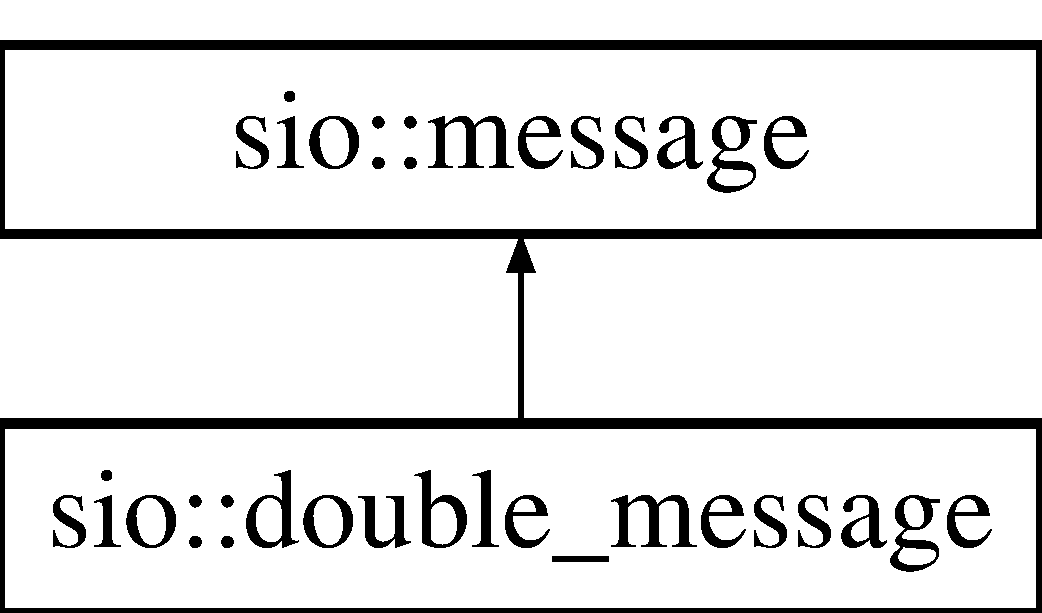
\includegraphics[height=2.000000cm]{classsio_1_1double__message}
\end{center}
\end{figure}
\subsection*{Public Member Functions}
\begin{DoxyCompactItemize}
\item 
double \hyperlink{classsio_1_1double__message_a0ab6e4c4e579356b367bb0ef37e79c62}{get\+\_\+double} () const
\end{DoxyCompactItemize}
\subsection*{Static Public Member Functions}
\begin{DoxyCompactItemize}
\item 
static \hyperlink{classsio_1_1message_a6340b6fef57e4516eb17928b1885a615}{message\+::ptr} \hyperlink{classsio_1_1double__message_a5bb130ec91b4b15f83bef32f5701054b}{create} (double v)
\end{DoxyCompactItemize}
\subsection*{Additional Inherited Members}


\subsection{Member Function Documentation}
\mbox{\Hypertarget{classsio_1_1double__message_a5bb130ec91b4b15f83bef32f5701054b}\label{classsio_1_1double__message_a5bb130ec91b4b15f83bef32f5701054b}} 
\index{sio\+::double\+\_\+message@{sio\+::double\+\_\+message}!create@{create}}
\index{create@{create}!sio\+::double\+\_\+message@{sio\+::double\+\_\+message}}
\subsubsection{\texorpdfstring{create()}{create()}}
{\footnotesize\ttfamily static \hyperlink{classsio_1_1message_a6340b6fef57e4516eb17928b1885a615}{message\+::ptr} sio\+::double\+\_\+message\+::create (\begin{DoxyParamCaption}\item[{double}]{v }\end{DoxyParamCaption})\hspace{0.3cm}{\ttfamily [inline]}, {\ttfamily [static]}}

\mbox{\Hypertarget{classsio_1_1double__message_a0ab6e4c4e579356b367bb0ef37e79c62}\label{classsio_1_1double__message_a0ab6e4c4e579356b367bb0ef37e79c62}} 
\index{sio\+::double\+\_\+message@{sio\+::double\+\_\+message}!get\+\_\+double@{get\+\_\+double}}
\index{get\+\_\+double@{get\+\_\+double}!sio\+::double\+\_\+message@{sio\+::double\+\_\+message}}
\subsubsection{\texorpdfstring{get\+\_\+double()}{get\_double()}}
{\footnotesize\ttfamily double sio\+::double\+\_\+message\+::get\+\_\+double (\begin{DoxyParamCaption}{ }\end{DoxyParamCaption}) const\hspace{0.3cm}{\ttfamily [inline]}, {\ttfamily [virtual]}}



Reimplemented from \hyperlink{classsio_1_1message_aa89963cd233b29653df1ce1943f9ea57}{sio\+::message}.



The documentation for this class was generated from the following file\+:\begin{DoxyCompactItemize}
\item 
/home/erik/work/bridges/bridges-\/cxx/src/\hyperlink{sio__message_8h}{sio\+\_\+message.\+h}\end{DoxyCompactItemize}

\hypertarget{classbridges_1_1dataset_1_1_earthquake_u_s_g_s}{}\section{bridges\+:\+:dataset\+:\+:Earthquake\+U\+S\+GS Class Reference}
\label{classbridges_1_1dataset_1_1_earthquake_u_s_g_s}\index{bridges\+::dataset\+::\+Earthquake\+U\+S\+GS@{bridges\+::dataset\+::\+Earthquake\+U\+S\+GS}}


{\ttfamily \#include $<$Earthquake\+U\+S\+G\+S.\+h$>$}



\subsection{Detailed Description}
Class that hold earthquake data, for use with U\+S\+G\+IS retrieved quake data. 

Class that holds earthquake U\+S\+G\+IS data. B\+R\+I\+D\+G\+ES uses scripts to continually monitor U\+S\+G\+IS site (tweets) and retrieve the latest quake data for use in student projects.

Kalpathi Subramanian, 2/18/18 \subsection*{Public Member Functions}
\begin{DoxyCompactItemize}
\item 
\mbox{\hyperlink{classbridges_1_1dataset_1_1_earthquake_u_s_g_s_a2e89f6ef9b631c6b8315c696cee7fb53}{Earthquake\+U\+S\+GS}} ()
\item 
\mbox{\hyperlink{classbridges_1_1dataset_1_1_earthquake_u_s_g_s_a3bb03ca9f4c0a3c8ecbab5a90b1886f8}{Earthquake\+U\+S\+GS}} (double magnitude, double longit, double latit, const string \&location, const string \&title, const string \&url, const string \&time)
\item 
\mbox{\hyperlink{classbridges_1_1dataset_1_1_earthquake_u_s_g_s_a382c751b8c71963ebcd7f0c7f1aed30a}{Earthquake\+U\+S\+GS}} (const \mbox{\hyperlink{classbridges_1_1dataset_1_1_earthquake_u_s_g_s}{Earthquake\+U\+S\+GS}} $\ast$eq)
\item 
string \mbox{\hyperlink{classbridges_1_1dataset_1_1_earthquake_u_s_g_s_a9078bfa4e954f78a3cf6e4a87747272b}{get\+Time}} () const
\begin{DoxyCompactList}\small\item\em return the epoch time of the quake \end{DoxyCompactList}\item 
string \mbox{\hyperlink{classbridges_1_1dataset_1_1_earthquake_u_s_g_s_a6fb0ff9a4f6cee9b1c04b588fc25c3ba}{get\+Date\+Str}} () const
\begin{DoxyCompactList}\small\item\em returns the real date in a string format \end{DoxyCompactList}\item 
void \mbox{\hyperlink{classbridges_1_1dataset_1_1_earthquake_u_s_g_s_af191301bcbaa5278480a57e9aea674d7}{set\+Time}} (const string \&tm)
\begin{DoxyCompactList}\small\item\em set epoch time \end{DoxyCompactList}\item 
int \mbox{\hyperlink{classbridges_1_1dataset_1_1_earthquake_u_s_g_s_a569120c9051d8d2fd73e3c778a81b9f3}{get\+Year}} () const
\begin{DoxyCompactList}\small\item\em get year of quake \end{DoxyCompactList}\item 
int \mbox{\hyperlink{classbridges_1_1dataset_1_1_earthquake_u_s_g_s_a010247e7474cc2434fff823a1a8b1142}{get\+Month}} () const
\begin{DoxyCompactList}\small\item\em get month of quake \end{DoxyCompactList}\item 
int \mbox{\hyperlink{classbridges_1_1dataset_1_1_earthquake_u_s_g_s_a6052793e29a4d9708ebf35cb8477ed0d}{get\+Day}} () const
\begin{DoxyCompactList}\small\item\em get day of quake \end{DoxyCompactList}\item 
int \mbox{\hyperlink{classbridges_1_1dataset_1_1_earthquake_u_s_g_s_a43e64f31d62d11ad554be5f5388720f6}{get\+Hour}} () const
\begin{DoxyCompactList}\small\item\em get hour of quake \end{DoxyCompactList}\item 
int \mbox{\hyperlink{classbridges_1_1dataset_1_1_earthquake_u_s_g_s_a2ca08fed1bfc867277dbd99cf25fa3ec}{get\+Minutes}} () const
\begin{DoxyCompactList}\small\item\em get minutes of quake \end{DoxyCompactList}\item 
int \mbox{\hyperlink{classbridges_1_1dataset_1_1_earthquake_u_s_g_s_af91ae1415cc7e0b82a5d288b7e033cd0}{get\+Seconds}} () const
\begin{DoxyCompactList}\small\item\em get seconds of quake \end{DoxyCompactList}\item 
float \mbox{\hyperlink{classbridges_1_1dataset_1_1_earthquake_u_s_g_s_aea3eca11487e572ead2ed91197d3d387}{get\+Latit}} () const
\begin{DoxyCompactList}\small\item\em get latitude of quake \end{DoxyCompactList}\item 
void \mbox{\hyperlink{classbridges_1_1dataset_1_1_earthquake_u_s_g_s_a68e7b4a3f74e57c574a5d09dc36a27ae}{set\+Latit}} (float latit)
\begin{DoxyCompactList}\small\item\em set latitude \end{DoxyCompactList}\item 
float \mbox{\hyperlink{classbridges_1_1dataset_1_1_earthquake_u_s_g_s_aab856d62ca076b54fff0e2b2a6b131d9}{get\+Longit}} () const
\begin{DoxyCompactList}\small\item\em get longitude of quake location \end{DoxyCompactList}\item 
void \mbox{\hyperlink{classbridges_1_1dataset_1_1_earthquake_u_s_g_s_a80ceea5c1ae15e7fd075ded145a14779}{set\+Longit}} (float longit)
\begin{DoxyCompactList}\small\item\em set longitude of quake location \end{DoxyCompactList}\item 
string \mbox{\hyperlink{classbridges_1_1dataset_1_1_earthquake_u_s_g_s_a56f3fede61e32b4bc35874435c59fc0e}{get\+Location}} () const
\begin{DoxyCompactList}\small\item\em get quake location. \end{DoxyCompactList}\item 
void \mbox{\hyperlink{classbridges_1_1dataset_1_1_earthquake_u_s_g_s_a88ad0700837cc78896eed2033e53d9a0}{set\+Location}} (string location)
\begin{DoxyCompactList}\small\item\em set quake location (string) \end{DoxyCompactList}\item 
string \mbox{\hyperlink{classbridges_1_1dataset_1_1_earthquake_u_s_g_s_a3e63533e53a119ceeb98c97ff35abc4a}{get\+Title}} () const
\begin{DoxyCompactList}\small\item\em get quake title \end{DoxyCompactList}\item 
void \mbox{\hyperlink{classbridges_1_1dataset_1_1_earthquake_u_s_g_s_a8a479d05e3f3896d4eeaad1bcccf9f02}{set\+Title}} (const string \&title)
\begin{DoxyCompactList}\small\item\em set quake title \end{DoxyCompactList}\item 
string \mbox{\hyperlink{classbridges_1_1dataset_1_1_earthquake_u_s_g_s_ab009982ed697df7ea2c913eb2b7e88be}{get\+Url}} () const
\begin{DoxyCompactList}\small\item\em get quake url \end{DoxyCompactList}\item 
void \mbox{\hyperlink{classbridges_1_1dataset_1_1_earthquake_u_s_g_s_aecb3cb7e4dba2315fed2a4a316a1fac9}{set\+Url}} (const string \&url)
\begin{DoxyCompactList}\small\item\em set quake url \end{DoxyCompactList}\item 
double \mbox{\hyperlink{classbridges_1_1dataset_1_1_earthquake_u_s_g_s_aeb1be6b0dece1240da3123db9f9c2d9b}{get\+Magnitude}} () const
\begin{DoxyCompactList}\small\item\em get quake magnitude \end{DoxyCompactList}\item 
void \mbox{\hyperlink{classbridges_1_1dataset_1_1_earthquake_u_s_g_s_ab961fcafd63f3ec0626ff38e2c4c01cd}{set\+Magnitude}} (double magnitude)
\begin{DoxyCompactList}\small\item\em set quake magnitude \end{DoxyCompactList}\end{DoxyCompactItemize}


\subsection{Constructor \& Destructor Documentation}
\mbox{\Hypertarget{classbridges_1_1dataset_1_1_earthquake_u_s_g_s_a2e89f6ef9b631c6b8315c696cee7fb53}\label{classbridges_1_1dataset_1_1_earthquake_u_s_g_s_a2e89f6ef9b631c6b8315c696cee7fb53}} 
\index{bridges\+::dataset\+::\+Earthquake\+U\+S\+GS@{bridges\+::dataset\+::\+Earthquake\+U\+S\+GS}!Earthquake\+U\+S\+GS@{Earthquake\+U\+S\+GS}}
\index{Earthquake\+U\+S\+GS@{Earthquake\+U\+S\+GS}!bridges\+::dataset\+::\+Earthquake\+U\+S\+GS@{bridges\+::dataset\+::\+Earthquake\+U\+S\+GS}}
\subsubsection{\texorpdfstring{Earthquake\+U\+S\+G\+S()}{EarthquakeUSGS()}\hspace{0.1cm}{\footnotesize\ttfamily [1/3]}}
{\footnotesize\ttfamily bridges\+::dataset\+::\+Earthquake\+U\+S\+G\+S\+::\+Earthquake\+U\+S\+GS (\begin{DoxyParamCaption}{ }\end{DoxyParamCaption})\hspace{0.3cm}{\ttfamily [inline]}}

\mbox{\Hypertarget{classbridges_1_1dataset_1_1_earthquake_u_s_g_s_a3bb03ca9f4c0a3c8ecbab5a90b1886f8}\label{classbridges_1_1dataset_1_1_earthquake_u_s_g_s_a3bb03ca9f4c0a3c8ecbab5a90b1886f8}} 
\index{bridges\+::dataset\+::\+Earthquake\+U\+S\+GS@{bridges\+::dataset\+::\+Earthquake\+U\+S\+GS}!Earthquake\+U\+S\+GS@{Earthquake\+U\+S\+GS}}
\index{Earthquake\+U\+S\+GS@{Earthquake\+U\+S\+GS}!bridges\+::dataset\+::\+Earthquake\+U\+S\+GS@{bridges\+::dataset\+::\+Earthquake\+U\+S\+GS}}
\subsubsection{\texorpdfstring{Earthquake\+U\+S\+G\+S()}{EarthquakeUSGS()}\hspace{0.1cm}{\footnotesize\ttfamily [2/3]}}
{\footnotesize\ttfamily bridges\+::dataset\+::\+Earthquake\+U\+S\+G\+S\+::\+Earthquake\+U\+S\+GS (\begin{DoxyParamCaption}\item[{double}]{magnitude,  }\item[{double}]{longit,  }\item[{double}]{latit,  }\item[{const string \&}]{location,  }\item[{const string \&}]{title,  }\item[{const string \&}]{url,  }\item[{const string \&}]{time }\end{DoxyParamCaption})\hspace{0.3cm}{\ttfamily [inline]}}

\mbox{\Hypertarget{classbridges_1_1dataset_1_1_earthquake_u_s_g_s_a382c751b8c71963ebcd7f0c7f1aed30a}\label{classbridges_1_1dataset_1_1_earthquake_u_s_g_s_a382c751b8c71963ebcd7f0c7f1aed30a}} 
\index{bridges\+::dataset\+::\+Earthquake\+U\+S\+GS@{bridges\+::dataset\+::\+Earthquake\+U\+S\+GS}!Earthquake\+U\+S\+GS@{Earthquake\+U\+S\+GS}}
\index{Earthquake\+U\+S\+GS@{Earthquake\+U\+S\+GS}!bridges\+::dataset\+::\+Earthquake\+U\+S\+GS@{bridges\+::dataset\+::\+Earthquake\+U\+S\+GS}}
\subsubsection{\texorpdfstring{Earthquake\+U\+S\+G\+S()}{EarthquakeUSGS()}\hspace{0.1cm}{\footnotesize\ttfamily [3/3]}}
{\footnotesize\ttfamily bridges\+::dataset\+::\+Earthquake\+U\+S\+G\+S\+::\+Earthquake\+U\+S\+GS (\begin{DoxyParamCaption}\item[{const \mbox{\hyperlink{classbridges_1_1dataset_1_1_earthquake_u_s_g_s}{Earthquake\+U\+S\+GS}} $\ast$}]{eq }\end{DoxyParamCaption})\hspace{0.3cm}{\ttfamily [inline]}}



\subsection{Member Function Documentation}
\mbox{\Hypertarget{classbridges_1_1dataset_1_1_earthquake_u_s_g_s_a6fb0ff9a4f6cee9b1c04b588fc25c3ba}\label{classbridges_1_1dataset_1_1_earthquake_u_s_g_s_a6fb0ff9a4f6cee9b1c04b588fc25c3ba}} 
\index{bridges\+::dataset\+::\+Earthquake\+U\+S\+GS@{bridges\+::dataset\+::\+Earthquake\+U\+S\+GS}!get\+Date\+Str@{get\+Date\+Str}}
\index{get\+Date\+Str@{get\+Date\+Str}!bridges\+::dataset\+::\+Earthquake\+U\+S\+GS@{bridges\+::dataset\+::\+Earthquake\+U\+S\+GS}}
\subsubsection{\texorpdfstring{get\+Date\+Str()}{getDateStr()}}
{\footnotesize\ttfamily string bridges\+::dataset\+::\+Earthquake\+U\+S\+G\+S\+::get\+Date\+Str (\begin{DoxyParamCaption}{ }\end{DoxyParamCaption}) const\hspace{0.3cm}{\ttfamily [inline]}}



returns the real date in a string format 

\begin{DoxyReturn}{Returns}
the real date in format \char`\"{}\+Month Day Year Hour\+:\+Minute\+:\+Seconds\char`\"{} 
\end{DoxyReturn}
\mbox{\Hypertarget{classbridges_1_1dataset_1_1_earthquake_u_s_g_s_a6052793e29a4d9708ebf35cb8477ed0d}\label{classbridges_1_1dataset_1_1_earthquake_u_s_g_s_a6052793e29a4d9708ebf35cb8477ed0d}} 
\index{bridges\+::dataset\+::\+Earthquake\+U\+S\+GS@{bridges\+::dataset\+::\+Earthquake\+U\+S\+GS}!get\+Day@{get\+Day}}
\index{get\+Day@{get\+Day}!bridges\+::dataset\+::\+Earthquake\+U\+S\+GS@{bridges\+::dataset\+::\+Earthquake\+U\+S\+GS}}
\subsubsection{\texorpdfstring{get\+Day()}{getDay()}}
{\footnotesize\ttfamily int bridges\+::dataset\+::\+Earthquake\+U\+S\+G\+S\+::get\+Day (\begin{DoxyParamCaption}{ }\end{DoxyParamCaption}) const\hspace{0.3cm}{\ttfamily [inline]}}



get day of quake 

\begin{DoxyReturn}{Returns}
day of the quake 
\end{DoxyReturn}
\mbox{\Hypertarget{classbridges_1_1dataset_1_1_earthquake_u_s_g_s_a43e64f31d62d11ad554be5f5388720f6}\label{classbridges_1_1dataset_1_1_earthquake_u_s_g_s_a43e64f31d62d11ad554be5f5388720f6}} 
\index{bridges\+::dataset\+::\+Earthquake\+U\+S\+GS@{bridges\+::dataset\+::\+Earthquake\+U\+S\+GS}!get\+Hour@{get\+Hour}}
\index{get\+Hour@{get\+Hour}!bridges\+::dataset\+::\+Earthquake\+U\+S\+GS@{bridges\+::dataset\+::\+Earthquake\+U\+S\+GS}}
\subsubsection{\texorpdfstring{get\+Hour()}{getHour()}}
{\footnotesize\ttfamily int bridges\+::dataset\+::\+Earthquake\+U\+S\+G\+S\+::get\+Hour (\begin{DoxyParamCaption}{ }\end{DoxyParamCaption}) const\hspace{0.3cm}{\ttfamily [inline]}}



get hour of quake 

\begin{DoxyReturn}{Returns}
hour of the quake 
\end{DoxyReturn}
\mbox{\Hypertarget{classbridges_1_1dataset_1_1_earthquake_u_s_g_s_aea3eca11487e572ead2ed91197d3d387}\label{classbridges_1_1dataset_1_1_earthquake_u_s_g_s_aea3eca11487e572ead2ed91197d3d387}} 
\index{bridges\+::dataset\+::\+Earthquake\+U\+S\+GS@{bridges\+::dataset\+::\+Earthquake\+U\+S\+GS}!get\+Latit@{get\+Latit}}
\index{get\+Latit@{get\+Latit}!bridges\+::dataset\+::\+Earthquake\+U\+S\+GS@{bridges\+::dataset\+::\+Earthquake\+U\+S\+GS}}
\subsubsection{\texorpdfstring{get\+Latit()}{getLatit()}}
{\footnotesize\ttfamily float bridges\+::dataset\+::\+Earthquake\+U\+S\+G\+S\+::get\+Latit (\begin{DoxyParamCaption}{ }\end{DoxyParamCaption}) const\hspace{0.3cm}{\ttfamily [inline]}}



get latitude of quake 

\begin{DoxyReturn}{Returns}
latitude of the quake 
\end{DoxyReturn}
\mbox{\Hypertarget{classbridges_1_1dataset_1_1_earthquake_u_s_g_s_a56f3fede61e32b4bc35874435c59fc0e}\label{classbridges_1_1dataset_1_1_earthquake_u_s_g_s_a56f3fede61e32b4bc35874435c59fc0e}} 
\index{bridges\+::dataset\+::\+Earthquake\+U\+S\+GS@{bridges\+::dataset\+::\+Earthquake\+U\+S\+GS}!get\+Location@{get\+Location}}
\index{get\+Location@{get\+Location}!bridges\+::dataset\+::\+Earthquake\+U\+S\+GS@{bridges\+::dataset\+::\+Earthquake\+U\+S\+GS}}
\subsubsection{\texorpdfstring{get\+Location()}{getLocation()}}
{\footnotesize\ttfamily string bridges\+::dataset\+::\+Earthquake\+U\+S\+G\+S\+::get\+Location (\begin{DoxyParamCaption}{ }\end{DoxyParamCaption}) const\hspace{0.3cm}{\ttfamily [inline]}}



get quake location. 

This is astring describing location (typically a city or something of the sort)

\begin{DoxyReturn}{Returns}
location as a string 
\end{DoxyReturn}
\mbox{\Hypertarget{classbridges_1_1dataset_1_1_earthquake_u_s_g_s_aab856d62ca076b54fff0e2b2a6b131d9}\label{classbridges_1_1dataset_1_1_earthquake_u_s_g_s_aab856d62ca076b54fff0e2b2a6b131d9}} 
\index{bridges\+::dataset\+::\+Earthquake\+U\+S\+GS@{bridges\+::dataset\+::\+Earthquake\+U\+S\+GS}!get\+Longit@{get\+Longit}}
\index{get\+Longit@{get\+Longit}!bridges\+::dataset\+::\+Earthquake\+U\+S\+GS@{bridges\+::dataset\+::\+Earthquake\+U\+S\+GS}}
\subsubsection{\texorpdfstring{get\+Longit()}{getLongit()}}
{\footnotesize\ttfamily float bridges\+::dataset\+::\+Earthquake\+U\+S\+G\+S\+::get\+Longit (\begin{DoxyParamCaption}{ }\end{DoxyParamCaption}) const\hspace{0.3cm}{\ttfamily [inline]}}



get longitude of quake location 

\begin{DoxyReturn}{Returns}
longitude of the quake 
\end{DoxyReturn}
\mbox{\Hypertarget{classbridges_1_1dataset_1_1_earthquake_u_s_g_s_aeb1be6b0dece1240da3123db9f9c2d9b}\label{classbridges_1_1dataset_1_1_earthquake_u_s_g_s_aeb1be6b0dece1240da3123db9f9c2d9b}} 
\index{bridges\+::dataset\+::\+Earthquake\+U\+S\+GS@{bridges\+::dataset\+::\+Earthquake\+U\+S\+GS}!get\+Magnitude@{get\+Magnitude}}
\index{get\+Magnitude@{get\+Magnitude}!bridges\+::dataset\+::\+Earthquake\+U\+S\+GS@{bridges\+::dataset\+::\+Earthquake\+U\+S\+GS}}
\subsubsection{\texorpdfstring{get\+Magnitude()}{getMagnitude()}}
{\footnotesize\ttfamily double bridges\+::dataset\+::\+Earthquake\+U\+S\+G\+S\+::get\+Magnitude (\begin{DoxyParamCaption}{ }\end{DoxyParamCaption}) const\hspace{0.3cm}{\ttfamily [inline]}}



get quake magnitude 

\begin{DoxyReturn}{Returns}
magnitude of the scale on Richter scale 
\end{DoxyReturn}
\mbox{\Hypertarget{classbridges_1_1dataset_1_1_earthquake_u_s_g_s_a2ca08fed1bfc867277dbd99cf25fa3ec}\label{classbridges_1_1dataset_1_1_earthquake_u_s_g_s_a2ca08fed1bfc867277dbd99cf25fa3ec}} 
\index{bridges\+::dataset\+::\+Earthquake\+U\+S\+GS@{bridges\+::dataset\+::\+Earthquake\+U\+S\+GS}!get\+Minutes@{get\+Minutes}}
\index{get\+Minutes@{get\+Minutes}!bridges\+::dataset\+::\+Earthquake\+U\+S\+GS@{bridges\+::dataset\+::\+Earthquake\+U\+S\+GS}}
\subsubsection{\texorpdfstring{get\+Minutes()}{getMinutes()}}
{\footnotesize\ttfamily int bridges\+::dataset\+::\+Earthquake\+U\+S\+G\+S\+::get\+Minutes (\begin{DoxyParamCaption}{ }\end{DoxyParamCaption}) const\hspace{0.3cm}{\ttfamily [inline]}}



get minutes of quake 

\begin{DoxyReturn}{Returns}
minutes of the quake 
\end{DoxyReturn}
\mbox{\Hypertarget{classbridges_1_1dataset_1_1_earthquake_u_s_g_s_a010247e7474cc2434fff823a1a8b1142}\label{classbridges_1_1dataset_1_1_earthquake_u_s_g_s_a010247e7474cc2434fff823a1a8b1142}} 
\index{bridges\+::dataset\+::\+Earthquake\+U\+S\+GS@{bridges\+::dataset\+::\+Earthquake\+U\+S\+GS}!get\+Month@{get\+Month}}
\index{get\+Month@{get\+Month}!bridges\+::dataset\+::\+Earthquake\+U\+S\+GS@{bridges\+::dataset\+::\+Earthquake\+U\+S\+GS}}
\subsubsection{\texorpdfstring{get\+Month()}{getMonth()}}
{\footnotesize\ttfamily int bridges\+::dataset\+::\+Earthquake\+U\+S\+G\+S\+::get\+Month (\begin{DoxyParamCaption}{ }\end{DoxyParamCaption}) const\hspace{0.3cm}{\ttfamily [inline]}}



get month of quake 

\begin{DoxyReturn}{Returns}
month of the quake 
\end{DoxyReturn}
\mbox{\Hypertarget{classbridges_1_1dataset_1_1_earthquake_u_s_g_s_af91ae1415cc7e0b82a5d288b7e033cd0}\label{classbridges_1_1dataset_1_1_earthquake_u_s_g_s_af91ae1415cc7e0b82a5d288b7e033cd0}} 
\index{bridges\+::dataset\+::\+Earthquake\+U\+S\+GS@{bridges\+::dataset\+::\+Earthquake\+U\+S\+GS}!get\+Seconds@{get\+Seconds}}
\index{get\+Seconds@{get\+Seconds}!bridges\+::dataset\+::\+Earthquake\+U\+S\+GS@{bridges\+::dataset\+::\+Earthquake\+U\+S\+GS}}
\subsubsection{\texorpdfstring{get\+Seconds()}{getSeconds()}}
{\footnotesize\ttfamily int bridges\+::dataset\+::\+Earthquake\+U\+S\+G\+S\+::get\+Seconds (\begin{DoxyParamCaption}{ }\end{DoxyParamCaption}) const\hspace{0.3cm}{\ttfamily [inline]}}



get seconds of quake 

\begin{DoxyReturn}{Returns}
get seconds of the quake 
\end{DoxyReturn}
\mbox{\Hypertarget{classbridges_1_1dataset_1_1_earthquake_u_s_g_s_a9078bfa4e954f78a3cf6e4a87747272b}\label{classbridges_1_1dataset_1_1_earthquake_u_s_g_s_a9078bfa4e954f78a3cf6e4a87747272b}} 
\index{bridges\+::dataset\+::\+Earthquake\+U\+S\+GS@{bridges\+::dataset\+::\+Earthquake\+U\+S\+GS}!get\+Time@{get\+Time}}
\index{get\+Time@{get\+Time}!bridges\+::dataset\+::\+Earthquake\+U\+S\+GS@{bridges\+::dataset\+::\+Earthquake\+U\+S\+GS}}
\subsubsection{\texorpdfstring{get\+Time()}{getTime()}}
{\footnotesize\ttfamily string bridges\+::dataset\+::\+Earthquake\+U\+S\+G\+S\+::get\+Time (\begin{DoxyParamCaption}{ }\end{DoxyParamCaption}) const\hspace{0.3cm}{\ttfamily [inline]}}



return the epoch time of the quake 

\begin{DoxyReturn}{Returns}
time 
\end{DoxyReturn}
\mbox{\Hypertarget{classbridges_1_1dataset_1_1_earthquake_u_s_g_s_a3e63533e53a119ceeb98c97ff35abc4a}\label{classbridges_1_1dataset_1_1_earthquake_u_s_g_s_a3e63533e53a119ceeb98c97ff35abc4a}} 
\index{bridges\+::dataset\+::\+Earthquake\+U\+S\+GS@{bridges\+::dataset\+::\+Earthquake\+U\+S\+GS}!get\+Title@{get\+Title}}
\index{get\+Title@{get\+Title}!bridges\+::dataset\+::\+Earthquake\+U\+S\+GS@{bridges\+::dataset\+::\+Earthquake\+U\+S\+GS}}
\subsubsection{\texorpdfstring{get\+Title()}{getTitle()}}
{\footnotesize\ttfamily string bridges\+::dataset\+::\+Earthquake\+U\+S\+G\+S\+::get\+Title (\begin{DoxyParamCaption}{ }\end{DoxyParamCaption}) const\hspace{0.3cm}{\ttfamily [inline]}}



get quake title 

Typically a one line description of the quake

\begin{DoxyReturn}{Returns}
title 
\end{DoxyReturn}
\mbox{\Hypertarget{classbridges_1_1dataset_1_1_earthquake_u_s_g_s_ab009982ed697df7ea2c913eb2b7e88be}\label{classbridges_1_1dataset_1_1_earthquake_u_s_g_s_ab009982ed697df7ea2c913eb2b7e88be}} 
\index{bridges\+::dataset\+::\+Earthquake\+U\+S\+GS@{bridges\+::dataset\+::\+Earthquake\+U\+S\+GS}!get\+Url@{get\+Url}}
\index{get\+Url@{get\+Url}!bridges\+::dataset\+::\+Earthquake\+U\+S\+GS@{bridges\+::dataset\+::\+Earthquake\+U\+S\+GS}}
\subsubsection{\texorpdfstring{get\+Url()}{getUrl()}}
{\footnotesize\ttfamily string bridges\+::dataset\+::\+Earthquake\+U\+S\+G\+S\+::get\+Url (\begin{DoxyParamCaption}{ }\end{DoxyParamCaption}) const\hspace{0.3cm}{\ttfamily [inline]}}



get quake url 

\begin{DoxyReturn}{Returns}
U\+S\+G\+IS url about the quake 
\end{DoxyReturn}
\mbox{\Hypertarget{classbridges_1_1dataset_1_1_earthquake_u_s_g_s_a569120c9051d8d2fd73e3c778a81b9f3}\label{classbridges_1_1dataset_1_1_earthquake_u_s_g_s_a569120c9051d8d2fd73e3c778a81b9f3}} 
\index{bridges\+::dataset\+::\+Earthquake\+U\+S\+GS@{bridges\+::dataset\+::\+Earthquake\+U\+S\+GS}!get\+Year@{get\+Year}}
\index{get\+Year@{get\+Year}!bridges\+::dataset\+::\+Earthquake\+U\+S\+GS@{bridges\+::dataset\+::\+Earthquake\+U\+S\+GS}}
\subsubsection{\texorpdfstring{get\+Year()}{getYear()}}
{\footnotesize\ttfamily int bridges\+::dataset\+::\+Earthquake\+U\+S\+G\+S\+::get\+Year (\begin{DoxyParamCaption}{ }\end{DoxyParamCaption}) const\hspace{0.3cm}{\ttfamily [inline]}}



get year of quake 

\begin{DoxyReturn}{Returns}
year of the quake 
\end{DoxyReturn}
\mbox{\Hypertarget{classbridges_1_1dataset_1_1_earthquake_u_s_g_s_a68e7b4a3f74e57c574a5d09dc36a27ae}\label{classbridges_1_1dataset_1_1_earthquake_u_s_g_s_a68e7b4a3f74e57c574a5d09dc36a27ae}} 
\index{bridges\+::dataset\+::\+Earthquake\+U\+S\+GS@{bridges\+::dataset\+::\+Earthquake\+U\+S\+GS}!set\+Latit@{set\+Latit}}
\index{set\+Latit@{set\+Latit}!bridges\+::dataset\+::\+Earthquake\+U\+S\+GS@{bridges\+::dataset\+::\+Earthquake\+U\+S\+GS}}
\subsubsection{\texorpdfstring{set\+Latit()}{setLatit()}}
{\footnotesize\ttfamily void bridges\+::dataset\+::\+Earthquake\+U\+S\+G\+S\+::set\+Latit (\begin{DoxyParamCaption}\item[{float}]{latit }\end{DoxyParamCaption})\hspace{0.3cm}{\ttfamily [inline]}}



set latitude 


\begin{DoxyParams}[1]{Parameters}
\mbox{\tt in}  & {\em latit} & latitude \\
\hline
\end{DoxyParams}
\mbox{\Hypertarget{classbridges_1_1dataset_1_1_earthquake_u_s_g_s_a88ad0700837cc78896eed2033e53d9a0}\label{classbridges_1_1dataset_1_1_earthquake_u_s_g_s_a88ad0700837cc78896eed2033e53d9a0}} 
\index{bridges\+::dataset\+::\+Earthquake\+U\+S\+GS@{bridges\+::dataset\+::\+Earthquake\+U\+S\+GS}!set\+Location@{set\+Location}}
\index{set\+Location@{set\+Location}!bridges\+::dataset\+::\+Earthquake\+U\+S\+GS@{bridges\+::dataset\+::\+Earthquake\+U\+S\+GS}}
\subsubsection{\texorpdfstring{set\+Location()}{setLocation()}}
{\footnotesize\ttfamily void bridges\+::dataset\+::\+Earthquake\+U\+S\+G\+S\+::set\+Location (\begin{DoxyParamCaption}\item[{string}]{location }\end{DoxyParamCaption})\hspace{0.3cm}{\ttfamily [inline]}}



set quake location (string) 


\begin{DoxyParams}[1]{Parameters}
\mbox{\tt in}  & {\em location} & location \\
\hline
\end{DoxyParams}
\mbox{\Hypertarget{classbridges_1_1dataset_1_1_earthquake_u_s_g_s_a80ceea5c1ae15e7fd075ded145a14779}\label{classbridges_1_1dataset_1_1_earthquake_u_s_g_s_a80ceea5c1ae15e7fd075ded145a14779}} 
\index{bridges\+::dataset\+::\+Earthquake\+U\+S\+GS@{bridges\+::dataset\+::\+Earthquake\+U\+S\+GS}!set\+Longit@{set\+Longit}}
\index{set\+Longit@{set\+Longit}!bridges\+::dataset\+::\+Earthquake\+U\+S\+GS@{bridges\+::dataset\+::\+Earthquake\+U\+S\+GS}}
\subsubsection{\texorpdfstring{set\+Longit()}{setLongit()}}
{\footnotesize\ttfamily void bridges\+::dataset\+::\+Earthquake\+U\+S\+G\+S\+::set\+Longit (\begin{DoxyParamCaption}\item[{float}]{longit }\end{DoxyParamCaption})\hspace{0.3cm}{\ttfamily [inline]}}



set longitude of quake location 


\begin{DoxyParams}[1]{Parameters}
\mbox{\tt in}  & {\em longit} & longitude of the quake \\
\hline
\end{DoxyParams}
\mbox{\Hypertarget{classbridges_1_1dataset_1_1_earthquake_u_s_g_s_ab961fcafd63f3ec0626ff38e2c4c01cd}\label{classbridges_1_1dataset_1_1_earthquake_u_s_g_s_ab961fcafd63f3ec0626ff38e2c4c01cd}} 
\index{bridges\+::dataset\+::\+Earthquake\+U\+S\+GS@{bridges\+::dataset\+::\+Earthquake\+U\+S\+GS}!set\+Magnitude@{set\+Magnitude}}
\index{set\+Magnitude@{set\+Magnitude}!bridges\+::dataset\+::\+Earthquake\+U\+S\+GS@{bridges\+::dataset\+::\+Earthquake\+U\+S\+GS}}
\subsubsection{\texorpdfstring{set\+Magnitude()}{setMagnitude()}}
{\footnotesize\ttfamily void bridges\+::dataset\+::\+Earthquake\+U\+S\+G\+S\+::set\+Magnitude (\begin{DoxyParamCaption}\item[{double}]{magnitude }\end{DoxyParamCaption})\hspace{0.3cm}{\ttfamily [inline]}}



set quake magnitude 


\begin{DoxyParams}[1]{Parameters}
\mbox{\tt in}  & {\em magnitude} & magnitude of the quake on Richter scale \\
\hline
\end{DoxyParams}
\mbox{\Hypertarget{classbridges_1_1dataset_1_1_earthquake_u_s_g_s_af191301bcbaa5278480a57e9aea674d7}\label{classbridges_1_1dataset_1_1_earthquake_u_s_g_s_af191301bcbaa5278480a57e9aea674d7}} 
\index{bridges\+::dataset\+::\+Earthquake\+U\+S\+GS@{bridges\+::dataset\+::\+Earthquake\+U\+S\+GS}!set\+Time@{set\+Time}}
\index{set\+Time@{set\+Time}!bridges\+::dataset\+::\+Earthquake\+U\+S\+GS@{bridges\+::dataset\+::\+Earthquake\+U\+S\+GS}}
\subsubsection{\texorpdfstring{set\+Time()}{setTime()}}
{\footnotesize\ttfamily void bridges\+::dataset\+::\+Earthquake\+U\+S\+G\+S\+::set\+Time (\begin{DoxyParamCaption}\item[{const string \&}]{tm }\end{DoxyParamCaption})\hspace{0.3cm}{\ttfamily [inline]}}



set epoch time 


\begin{DoxyParams}{Parameters}
{\em tm} & time as epoch \\
\hline
\end{DoxyParams}
\mbox{\Hypertarget{classbridges_1_1dataset_1_1_earthquake_u_s_g_s_a8a479d05e3f3896d4eeaad1bcccf9f02}\label{classbridges_1_1dataset_1_1_earthquake_u_s_g_s_a8a479d05e3f3896d4eeaad1bcccf9f02}} 
\index{bridges\+::dataset\+::\+Earthquake\+U\+S\+GS@{bridges\+::dataset\+::\+Earthquake\+U\+S\+GS}!set\+Title@{set\+Title}}
\index{set\+Title@{set\+Title}!bridges\+::dataset\+::\+Earthquake\+U\+S\+GS@{bridges\+::dataset\+::\+Earthquake\+U\+S\+GS}}
\subsubsection{\texorpdfstring{set\+Title()}{setTitle()}}
{\footnotesize\ttfamily void bridges\+::dataset\+::\+Earthquake\+U\+S\+G\+S\+::set\+Title (\begin{DoxyParamCaption}\item[{const string \&}]{title }\end{DoxyParamCaption})\hspace{0.3cm}{\ttfamily [inline]}}



set quake title 


\begin{DoxyParams}[1]{Parameters}
\mbox{\tt in}  & {\em title} & quake title \\
\hline
\end{DoxyParams}
\mbox{\Hypertarget{classbridges_1_1dataset_1_1_earthquake_u_s_g_s_aecb3cb7e4dba2315fed2a4a316a1fac9}\label{classbridges_1_1dataset_1_1_earthquake_u_s_g_s_aecb3cb7e4dba2315fed2a4a316a1fac9}} 
\index{bridges\+::dataset\+::\+Earthquake\+U\+S\+GS@{bridges\+::dataset\+::\+Earthquake\+U\+S\+GS}!set\+Url@{set\+Url}}
\index{set\+Url@{set\+Url}!bridges\+::dataset\+::\+Earthquake\+U\+S\+GS@{bridges\+::dataset\+::\+Earthquake\+U\+S\+GS}}
\subsubsection{\texorpdfstring{set\+Url()}{setUrl()}}
{\footnotesize\ttfamily void bridges\+::dataset\+::\+Earthquake\+U\+S\+G\+S\+::set\+Url (\begin{DoxyParamCaption}\item[{const string \&}]{url }\end{DoxyParamCaption})\hspace{0.3cm}{\ttfamily [inline]}}



set quake url 


\begin{DoxyParams}[1]{Parameters}
\mbox{\tt in}  & {\em url} & U\+S\+G\+IS url of the quake \\
\hline
\end{DoxyParams}


The documentation for this class was generated from the following file\+:\begin{DoxyCompactItemize}
\item 
/\+Users/kalpathi/gr/bridges/client/cxx/src/data\+\_\+src/\mbox{\hyperlink{_earthquake_u_s_g_s_8h}{Earthquake\+U\+S\+G\+S.\+h}}\end{DoxyCompactItemize}

\hypertarget{classbridges_1_1datastructure_1_1_edge}{}\doxysection{bridges\+::datastructure\+::Edge$<$ K, E2 $>$ Class Template Reference}
\label{classbridges_1_1datastructure_1_1_edge}\index{bridges::datastructure::Edge$<$ K, E2 $>$@{bridges::datastructure::Edge$<$ K, E2 $>$}}


{\ttfamily \#include $<$Edge.\+h$>$}



\doxysubsection{Detailed Description}
\subsubsection*{template$<$typename K, typename E2 = K$>$\newline
class bridges\+::datastructure\+::\+Edge$<$ K, E2 $>$}

This helper class is used by the graph classes -\/ \mbox{\hyperlink{classbridges_1_1datastructure_1_1_graph_adj_list}{Graph\+Adj\+List}} , \mbox{\hyperlink{classbridges_1_1datastructure_1_1_graph_adj_matrix}{Graph\+Adj\+Matrix}} -\/ to keep track of edge information. 

This class is used to assign a visual connection between two Elements in the \mbox{\hyperlink{classbridges_1_1_bridges}{Bridges}} Visualization.

\mbox{\hyperlink{classbridges_1_1_bridges}{Bridges}} will represent these as arrows between two Elements. The starting \mbox{\hyperlink{classbridges_1_1datastructure_1_1_element}{Element}} of the arrow will be referred to as the source \mbox{\hyperlink{classbridges_1_1datastructure_1_1_element}{Element}} and the ending \mbox{\hyperlink{classbridges_1_1datastructure_1_1_element}{Element}} of the arrow will be referred to as the terminating \mbox{\hyperlink{classbridges_1_1datastructure_1_1_element}{Element}}.

\begin{DoxyAuthor}{Author}
Kalpathi Subramanian, Erik Saule
\end{DoxyAuthor}
\begin{DoxyDate}{Date}
12/28/20
\end{DoxyDate}

\begin{DoxyParams}{Parameters}
{\em E} & \\
\hline
\end{DoxyParams}
\doxysubsection*{Public Member Functions}
\begin{DoxyCompactItemize}
\item 
\mbox{\hyperlink{classbridges_1_1datastructure_1_1_edge_aae44cef647b20d260b449a5fb041ae95}{Edge}} (const K \&\mbox{\hyperlink{classbridges_1_1datastructure_1_1_edge_a0fba8af11c12f73c993f6e8a573daa02}{from}}, const K \&\mbox{\hyperlink{classbridges_1_1datastructure_1_1_edge_a2cece2762a29e3fc18859e0c725eee82}{to}}, \mbox{\hyperlink{classbridges_1_1datastructure_1_1_link_visualizer}{Link\+Visualizer}} $\ast$lv, const E2 \&data=E2())
\begin{DoxyCompactList}\small\item\em Constructs an edge with the given destination vertex, and edge data. \end{DoxyCompactList}\item 
\mbox{\hyperlink{classbridges_1_1datastructure_1_1_edge_a7160632622b92c93036cd6fdcec75959}{$\sim$\+Edge}} ()
\item 
const K \& \mbox{\hyperlink{classbridges_1_1datastructure_1_1_edge_a0fba8af11c12f73c993f6e8a573daa02}{from}} () const
\begin{DoxyCompactList}\small\item\em Source vertex accessor. \end{DoxyCompactList}\item 
const K \& \mbox{\hyperlink{classbridges_1_1datastructure_1_1_edge_a2cece2762a29e3fc18859e0c725eee82}{to}} () const
\begin{DoxyCompactList}\small\item\em Destination vertex accessor. \end{DoxyCompactList}\item 
void \mbox{\hyperlink{classbridges_1_1datastructure_1_1_edge_a8f030413780f15f90141e4ff29240ec0}{set\+Edge\+Data}} (const E2 \&data)
\begin{DoxyCompactList}\small\item\em Sets edge data to \char`\"{}data\char`\"{}. \end{DoxyCompactList}\item 
const E2 \& \mbox{\hyperlink{classbridges_1_1datastructure_1_1_edge_a4769b5d8fc74522f77f5927b230ced7b}{get\+Edge\+Data}} () const
\begin{DoxyCompactList}\small\item\em Return the edge data. \end{DoxyCompactList}\item 
E2 \& \mbox{\hyperlink{classbridges_1_1datastructure_1_1_edge_a302b605a5d30387cfae8f4805c43ec41}{get\+Edge\+Data}} ()
\begin{DoxyCompactList}\small\item\em Return the edge data. \end{DoxyCompactList}\item 
string \mbox{\hyperlink{classbridges_1_1datastructure_1_1_edge_aad4a9a28e282e5aa5e7821a14ef94327}{get\+Label}} () const
\begin{DoxyCompactList}\small\item\em Return the edge label. \end{DoxyCompactList}\item 
void \mbox{\hyperlink{classbridges_1_1datastructure_1_1_edge_a5f88c4db54027da70de06f21fd5b6ccd}{set\+Label}} (const string \&lab)
\begin{DoxyCompactList}\small\item\em Sets edge label to \char`\"{}lab\char`\"{}. \end{DoxyCompactList}\item 
void \mbox{\hyperlink{classbridges_1_1datastructure_1_1_edge_adf4a6a3974e1fc60331f4b9d33c7b0e5}{set\+Thickness}} (const double \&th)
\begin{DoxyCompactList}\small\item\em Change the thickness of the edge when displayed. \end{DoxyCompactList}\item 
double \mbox{\hyperlink{classbridges_1_1datastructure_1_1_edge_a6163e53061d4785b969fa664dbae104b}{get\+Thickness}} () const
\begin{DoxyCompactList}\small\item\em Get the thickness of the edge. \end{DoxyCompactList}\item 
void \mbox{\hyperlink{classbridges_1_1datastructure_1_1_edge_a9eab71fed936587b2a3109d3df3c46fb}{set\+Color}} (const \mbox{\hyperlink{classbridges_1_1datastructure_1_1_color}{Color}} \&col)
\begin{DoxyCompactList}\small\item\em Set the color of the edge. \end{DoxyCompactList}\item 
void \mbox{\hyperlink{classbridges_1_1datastructure_1_1_edge_a5a38f46e9662624af4de9fcf596c4783}{set\+Color}} (const string col)
\begin{DoxyCompactList}\small\item\em Set the color to a named color. Check the \mbox{\hyperlink{classbridges_1_1datastructure_1_1_color}{Color}} class for a list of named colors. \end{DoxyCompactList}\item 
\mbox{\hyperlink{classbridges_1_1datastructure_1_1_color}{Color}} \mbox{\hyperlink{classbridges_1_1datastructure_1_1_edge_abb5c66b734e1ac71e5d4e012908ec7a4}{get\+Color}} () const
\begin{DoxyCompactList}\small\item\em return the current color of the edge \end{DoxyCompactList}\item 
\mbox{\hyperlink{classbridges_1_1datastructure_1_1_link_visualizer}{Link\+Visualizer}} $\ast$ \mbox{\hyperlink{classbridges_1_1datastructure_1_1_edge_a0470604705c93dd33b382a70d5c78f93}{get\+Link\+Visualizer}} ()
\begin{DoxyCompactList}\small\item\em Get the link visualizer of this edge. \end{DoxyCompactList}\end{DoxyCompactItemize}


\doxysubsection{Constructor \& Destructor Documentation}
\mbox{\Hypertarget{classbridges_1_1datastructure_1_1_edge_aae44cef647b20d260b449a5fb041ae95}\label{classbridges_1_1datastructure_1_1_edge_aae44cef647b20d260b449a5fb041ae95}} 
\index{bridges::datastructure::Edge$<$ K, E2 $>$@{bridges::datastructure::Edge$<$ K, E2 $>$}!Edge@{Edge}}
\index{Edge@{Edge}!bridges::datastructure::Edge$<$ K, E2 $>$@{bridges::datastructure::Edge$<$ K, E2 $>$}}
\doxysubsubsection{\texorpdfstring{Edge()}{Edge()}}
{\footnotesize\ttfamily template$<$typename K , typename E2  = K$>$ \\
\mbox{\hyperlink{classbridges_1_1datastructure_1_1_edge}{bridges\+::datastructure\+::\+Edge}}$<$ K, E2 $>$\+::\mbox{\hyperlink{classbridges_1_1datastructure_1_1_edge}{Edge}} (\begin{DoxyParamCaption}\item[{const K \&}]{from,  }\item[{const K \&}]{to,  }\item[{\mbox{\hyperlink{classbridges_1_1datastructure_1_1_link_visualizer}{Link\+Visualizer}} $\ast$}]{lv,  }\item[{const E2 \&}]{data = {\ttfamily E2()} }\end{DoxyParamCaption})\hspace{0.3cm}{\ttfamily [inline]}}



Constructs an edge with the given destination vertex, and edge data. 

This constructor is not meant to be used by the \mbox{\hyperlink{classbridges_1_1_bridges}{Bridges}} user. If an argument is not given its default is used.


\begin{DoxyParams}{Parameters}
{\em from} & source vertex \\
\hline
{\em to} & destination vertex \\
\hline
{\em lv} & \mbox{\hyperlink{classbridges_1_1datastructure_1_1_link_visualizer}{Link\+Visualizer}} storing the styling information for the edge \\
\hline
{\em data} & edge data \\
\hline
\end{DoxyParams}
\mbox{\Hypertarget{classbridges_1_1datastructure_1_1_edge_a7160632622b92c93036cd6fdcec75959}\label{classbridges_1_1datastructure_1_1_edge_a7160632622b92c93036cd6fdcec75959}} 
\index{bridges::datastructure::Edge$<$ K, E2 $>$@{bridges::datastructure::Edge$<$ K, E2 $>$}!````~Edge@{$\sim$Edge}}
\index{````~Edge@{$\sim$Edge}!bridges::datastructure::Edge$<$ K, E2 $>$@{bridges::datastructure::Edge$<$ K, E2 $>$}}
\doxysubsubsection{\texorpdfstring{$\sim$Edge()}{~Edge()}}
{\footnotesize\ttfamily template$<$typename K , typename E2  = K$>$ \\
\mbox{\hyperlink{classbridges_1_1datastructure_1_1_edge}{bridges\+::datastructure\+::\+Edge}}$<$ K, E2 $>$\+::$\sim$\mbox{\hyperlink{classbridges_1_1datastructure_1_1_edge}{Edge}} (\begin{DoxyParamCaption}{ }\end{DoxyParamCaption})\hspace{0.3cm}{\ttfamily [inline]}}



\doxysubsection{Member Function Documentation}
\mbox{\Hypertarget{classbridges_1_1datastructure_1_1_edge_a0fba8af11c12f73c993f6e8a573daa02}\label{classbridges_1_1datastructure_1_1_edge_a0fba8af11c12f73c993f6e8a573daa02}} 
\index{bridges::datastructure::Edge$<$ K, E2 $>$@{bridges::datastructure::Edge$<$ K, E2 $>$}!from@{from}}
\index{from@{from}!bridges::datastructure::Edge$<$ K, E2 $>$@{bridges::datastructure::Edge$<$ K, E2 $>$}}
\doxysubsubsection{\texorpdfstring{from()}{from()}}
{\footnotesize\ttfamily template$<$typename K , typename E2  = K$>$ \\
const K\& \mbox{\hyperlink{classbridges_1_1datastructure_1_1_edge}{bridges\+::datastructure\+::\+Edge}}$<$ K, E2 $>$\+::from (\begin{DoxyParamCaption}{ }\end{DoxyParamCaption}) const\hspace{0.3cm}{\ttfamily [inline]}}



Source vertex accessor. 

\begin{DoxyReturn}{Returns}
The source vertex 
\end{DoxyReturn}
\mbox{\Hypertarget{classbridges_1_1datastructure_1_1_edge_abb5c66b734e1ac71e5d4e012908ec7a4}\label{classbridges_1_1datastructure_1_1_edge_abb5c66b734e1ac71e5d4e012908ec7a4}} 
\index{bridges::datastructure::Edge$<$ K, E2 $>$@{bridges::datastructure::Edge$<$ K, E2 $>$}!getColor@{getColor}}
\index{getColor@{getColor}!bridges::datastructure::Edge$<$ K, E2 $>$@{bridges::datastructure::Edge$<$ K, E2 $>$}}
\doxysubsubsection{\texorpdfstring{getColor()}{getColor()}}
{\footnotesize\ttfamily template$<$typename K , typename E2  = K$>$ \\
\mbox{\hyperlink{classbridges_1_1datastructure_1_1_color}{Color}} \mbox{\hyperlink{classbridges_1_1datastructure_1_1_edge}{bridges\+::datastructure\+::\+Edge}}$<$ K, E2 $>$\+::get\+Color (\begin{DoxyParamCaption}{ }\end{DoxyParamCaption}) const\hspace{0.3cm}{\ttfamily [inline]}}



return the current color of the edge 

\begin{DoxyReturn}{Returns}
The color of the edge 
\end{DoxyReturn}
\mbox{\Hypertarget{classbridges_1_1datastructure_1_1_edge_a302b605a5d30387cfae8f4805c43ec41}\label{classbridges_1_1datastructure_1_1_edge_a302b605a5d30387cfae8f4805c43ec41}} 
\index{bridges::datastructure::Edge$<$ K, E2 $>$@{bridges::datastructure::Edge$<$ K, E2 $>$}!getEdgeData@{getEdgeData}}
\index{getEdgeData@{getEdgeData}!bridges::datastructure::Edge$<$ K, E2 $>$@{bridges::datastructure::Edge$<$ K, E2 $>$}}
\doxysubsubsection{\texorpdfstring{getEdgeData()}{getEdgeData()}\hspace{0.1cm}{\footnotesize\ttfamily [1/2]}}
{\footnotesize\ttfamily template$<$typename K , typename E2  = K$>$ \\
E2\& \mbox{\hyperlink{classbridges_1_1datastructure_1_1_edge}{bridges\+::datastructure\+::\+Edge}}$<$ K, E2 $>$\+::get\+Edge\+Data (\begin{DoxyParamCaption}{ }\end{DoxyParamCaption})\hspace{0.3cm}{\ttfamily [inline]}}



Return the edge data. 

\begin{DoxyReturn}{Returns}
The edge data 
\end{DoxyReturn}
\mbox{\Hypertarget{classbridges_1_1datastructure_1_1_edge_a4769b5d8fc74522f77f5927b230ced7b}\label{classbridges_1_1datastructure_1_1_edge_a4769b5d8fc74522f77f5927b230ced7b}} 
\index{bridges::datastructure::Edge$<$ K, E2 $>$@{bridges::datastructure::Edge$<$ K, E2 $>$}!getEdgeData@{getEdgeData}}
\index{getEdgeData@{getEdgeData}!bridges::datastructure::Edge$<$ K, E2 $>$@{bridges::datastructure::Edge$<$ K, E2 $>$}}
\doxysubsubsection{\texorpdfstring{getEdgeData()}{getEdgeData()}\hspace{0.1cm}{\footnotesize\ttfamily [2/2]}}
{\footnotesize\ttfamily template$<$typename K , typename E2  = K$>$ \\
const E2\& \mbox{\hyperlink{classbridges_1_1datastructure_1_1_edge}{bridges\+::datastructure\+::\+Edge}}$<$ K, E2 $>$\+::get\+Edge\+Data (\begin{DoxyParamCaption}{ }\end{DoxyParamCaption}) const\hspace{0.3cm}{\ttfamily [inline]}}



Return the edge data. 

\begin{DoxyReturn}{Returns}
The edge data 
\end{DoxyReturn}
\mbox{\Hypertarget{classbridges_1_1datastructure_1_1_edge_aad4a9a28e282e5aa5e7821a14ef94327}\label{classbridges_1_1datastructure_1_1_edge_aad4a9a28e282e5aa5e7821a14ef94327}} 
\index{bridges::datastructure::Edge$<$ K, E2 $>$@{bridges::datastructure::Edge$<$ K, E2 $>$}!getLabel@{getLabel}}
\index{getLabel@{getLabel}!bridges::datastructure::Edge$<$ K, E2 $>$@{bridges::datastructure::Edge$<$ K, E2 $>$}}
\doxysubsubsection{\texorpdfstring{getLabel()}{getLabel()}}
{\footnotesize\ttfamily template$<$typename K , typename E2  = K$>$ \\
string \mbox{\hyperlink{classbridges_1_1datastructure_1_1_edge}{bridges\+::datastructure\+::\+Edge}}$<$ K, E2 $>$\+::get\+Label (\begin{DoxyParamCaption}{ }\end{DoxyParamCaption}) const\hspace{0.3cm}{\ttfamily [inline]}}



Return the edge label. 

\begin{DoxyReturn}{Returns}
The label of the element 
\end{DoxyReturn}
\mbox{\Hypertarget{classbridges_1_1datastructure_1_1_edge_a0470604705c93dd33b382a70d5c78f93}\label{classbridges_1_1datastructure_1_1_edge_a0470604705c93dd33b382a70d5c78f93}} 
\index{bridges::datastructure::Edge$<$ K, E2 $>$@{bridges::datastructure::Edge$<$ K, E2 $>$}!getLinkVisualizer@{getLinkVisualizer}}
\index{getLinkVisualizer@{getLinkVisualizer}!bridges::datastructure::Edge$<$ K, E2 $>$@{bridges::datastructure::Edge$<$ K, E2 $>$}}
\doxysubsubsection{\texorpdfstring{getLinkVisualizer()}{getLinkVisualizer()}}
{\footnotesize\ttfamily template$<$typename K , typename E2  = K$>$ \\
\mbox{\hyperlink{classbridges_1_1datastructure_1_1_link_visualizer}{Link\+Visualizer}}$\ast$ \mbox{\hyperlink{classbridges_1_1datastructure_1_1_edge}{bridges\+::datastructure\+::\+Edge}}$<$ K, E2 $>$\+::get\+Link\+Visualizer (\begin{DoxyParamCaption}{ }\end{DoxyParamCaption})\hspace{0.3cm}{\ttfamily [inline]}}



Get the link visualizer of this edge. 

\begin{DoxyReturn}{Returns}
return the link visualizer of this edge 
\end{DoxyReturn}
\mbox{\Hypertarget{classbridges_1_1datastructure_1_1_edge_a6163e53061d4785b969fa664dbae104b}\label{classbridges_1_1datastructure_1_1_edge_a6163e53061d4785b969fa664dbae104b}} 
\index{bridges::datastructure::Edge$<$ K, E2 $>$@{bridges::datastructure::Edge$<$ K, E2 $>$}!getThickness@{getThickness}}
\index{getThickness@{getThickness}!bridges::datastructure::Edge$<$ K, E2 $>$@{bridges::datastructure::Edge$<$ K, E2 $>$}}
\doxysubsubsection{\texorpdfstring{getThickness()}{getThickness()}}
{\footnotesize\ttfamily template$<$typename K , typename E2  = K$>$ \\
double \mbox{\hyperlink{classbridges_1_1datastructure_1_1_edge}{bridges\+::datastructure\+::\+Edge}}$<$ K, E2 $>$\+::get\+Thickness (\begin{DoxyParamCaption}{ }\end{DoxyParamCaption}) const\hspace{0.3cm}{\ttfamily [inline]}}



Get the thickness of the edge. 

\begin{DoxyReturn}{Returns}
Size in pixels of the link\textquotesingle{}s line thickness 
\end{DoxyReturn}
\mbox{\Hypertarget{classbridges_1_1datastructure_1_1_edge_a9eab71fed936587b2a3109d3df3c46fb}\label{classbridges_1_1datastructure_1_1_edge_a9eab71fed936587b2a3109d3df3c46fb}} 
\index{bridges::datastructure::Edge$<$ K, E2 $>$@{bridges::datastructure::Edge$<$ K, E2 $>$}!setColor@{setColor}}
\index{setColor@{setColor}!bridges::datastructure::Edge$<$ K, E2 $>$@{bridges::datastructure::Edge$<$ K, E2 $>$}}
\doxysubsubsection{\texorpdfstring{setColor()}{setColor()}\hspace{0.1cm}{\footnotesize\ttfamily [1/2]}}
{\footnotesize\ttfamily template$<$typename K , typename E2  = K$>$ \\
void \mbox{\hyperlink{classbridges_1_1datastructure_1_1_edge}{bridges\+::datastructure\+::\+Edge}}$<$ K, E2 $>$\+::set\+Color (\begin{DoxyParamCaption}\item[{const \mbox{\hyperlink{classbridges_1_1datastructure_1_1_color}{Color}} \&}]{col }\end{DoxyParamCaption})\hspace{0.3cm}{\ttfamily [inline]}}



Set the color of the edge. 


\begin{DoxyParams}{Parameters}
{\em col} & The color of the edge \\
\hline
\end{DoxyParams}
\mbox{\Hypertarget{classbridges_1_1datastructure_1_1_edge_a5a38f46e9662624af4de9fcf596c4783}\label{classbridges_1_1datastructure_1_1_edge_a5a38f46e9662624af4de9fcf596c4783}} 
\index{bridges::datastructure::Edge$<$ K, E2 $>$@{bridges::datastructure::Edge$<$ K, E2 $>$}!setColor@{setColor}}
\index{setColor@{setColor}!bridges::datastructure::Edge$<$ K, E2 $>$@{bridges::datastructure::Edge$<$ K, E2 $>$}}
\doxysubsubsection{\texorpdfstring{setColor()}{setColor()}\hspace{0.1cm}{\footnotesize\ttfamily [2/2]}}
{\footnotesize\ttfamily template$<$typename K , typename E2  = K$>$ \\
void \mbox{\hyperlink{classbridges_1_1datastructure_1_1_edge}{bridges\+::datastructure\+::\+Edge}}$<$ K, E2 $>$\+::set\+Color (\begin{DoxyParamCaption}\item[{const string}]{col }\end{DoxyParamCaption})\hspace{0.3cm}{\ttfamily [inline]}}



Set the color to a named color. Check the \mbox{\hyperlink{classbridges_1_1datastructure_1_1_color}{Color}} class for a list of named colors. 


\begin{DoxyParams}{Parameters}
{\em col} & The name of the color. \\
\hline
\end{DoxyParams}
\mbox{\Hypertarget{classbridges_1_1datastructure_1_1_edge_a8f030413780f15f90141e4ff29240ec0}\label{classbridges_1_1datastructure_1_1_edge_a8f030413780f15f90141e4ff29240ec0}} 
\index{bridges::datastructure::Edge$<$ K, E2 $>$@{bridges::datastructure::Edge$<$ K, E2 $>$}!setEdgeData@{setEdgeData}}
\index{setEdgeData@{setEdgeData}!bridges::datastructure::Edge$<$ K, E2 $>$@{bridges::datastructure::Edge$<$ K, E2 $>$}}
\doxysubsubsection{\texorpdfstring{setEdgeData()}{setEdgeData()}}
{\footnotesize\ttfamily template$<$typename K , typename E2  = K$>$ \\
void \mbox{\hyperlink{classbridges_1_1datastructure_1_1_edge}{bridges\+::datastructure\+::\+Edge}}$<$ K, E2 $>$\+::set\+Edge\+Data (\begin{DoxyParamCaption}\item[{const E2 \&}]{data }\end{DoxyParamCaption})\hspace{0.3cm}{\ttfamily [inline]}}



Sets edge data to \char`\"{}data\char`\"{}. 


\begin{DoxyParams}{Parameters}
{\em data} & Application data to be set \\
\hline
\end{DoxyParams}
\mbox{\Hypertarget{classbridges_1_1datastructure_1_1_edge_a5f88c4db54027da70de06f21fd5b6ccd}\label{classbridges_1_1datastructure_1_1_edge_a5f88c4db54027da70de06f21fd5b6ccd}} 
\index{bridges::datastructure::Edge$<$ K, E2 $>$@{bridges::datastructure::Edge$<$ K, E2 $>$}!setLabel@{setLabel}}
\index{setLabel@{setLabel}!bridges::datastructure::Edge$<$ K, E2 $>$@{bridges::datastructure::Edge$<$ K, E2 $>$}}
\doxysubsubsection{\texorpdfstring{setLabel()}{setLabel()}}
{\footnotesize\ttfamily template$<$typename K , typename E2  = K$>$ \\
void \mbox{\hyperlink{classbridges_1_1datastructure_1_1_edge}{bridges\+::datastructure\+::\+Edge}}$<$ K, E2 $>$\+::set\+Label (\begin{DoxyParamCaption}\item[{const string \&}]{lab }\end{DoxyParamCaption})\hspace{0.3cm}{\ttfamily [inline]}}



Sets edge label to \char`\"{}lab\char`\"{}. 


\begin{DoxyParams}{Parameters}
{\em lab} & The label of the element \\
\hline
\end{DoxyParams}
\mbox{\Hypertarget{classbridges_1_1datastructure_1_1_edge_adf4a6a3974e1fc60331f4b9d33c7b0e5}\label{classbridges_1_1datastructure_1_1_edge_adf4a6a3974e1fc60331f4b9d33c7b0e5}} 
\index{bridges::datastructure::Edge$<$ K, E2 $>$@{bridges::datastructure::Edge$<$ K, E2 $>$}!setThickness@{setThickness}}
\index{setThickness@{setThickness}!bridges::datastructure::Edge$<$ K, E2 $>$@{bridges::datastructure::Edge$<$ K, E2 $>$}}
\doxysubsubsection{\texorpdfstring{setThickness()}{setThickness()}}
{\footnotesize\ttfamily template$<$typename K , typename E2  = K$>$ \\
void \mbox{\hyperlink{classbridges_1_1datastructure_1_1_edge}{bridges\+::datastructure\+::\+Edge}}$<$ K, E2 $>$\+::set\+Thickness (\begin{DoxyParamCaption}\item[{const double \&}]{th }\end{DoxyParamCaption})\hspace{0.3cm}{\ttfamily [inline]}}



Change the thickness of the edge when displayed. 

Valid Range\+:\mbox{[}1,10\mbox{]} Default\+: 1


\begin{DoxyParams}{Parameters}
{\em th} & The size in pixels of the link\textquotesingle{}s line weight \\
\hline
\end{DoxyParams}

\begin{DoxyExceptions}{Exceptions}
{\em string} & If invalid thickness \\
\hline
\end{DoxyExceptions}
\mbox{\Hypertarget{classbridges_1_1datastructure_1_1_edge_a2cece2762a29e3fc18859e0c725eee82}\label{classbridges_1_1datastructure_1_1_edge_a2cece2762a29e3fc18859e0c725eee82}} 
\index{bridges::datastructure::Edge$<$ K, E2 $>$@{bridges::datastructure::Edge$<$ K, E2 $>$}!to@{to}}
\index{to@{to}!bridges::datastructure::Edge$<$ K, E2 $>$@{bridges::datastructure::Edge$<$ K, E2 $>$}}
\doxysubsubsection{\texorpdfstring{to()}{to()}}
{\footnotesize\ttfamily template$<$typename K , typename E2  = K$>$ \\
const K\& \mbox{\hyperlink{classbridges_1_1datastructure_1_1_edge}{bridges\+::datastructure\+::\+Edge}}$<$ K, E2 $>$\+::to (\begin{DoxyParamCaption}{ }\end{DoxyParamCaption}) const\hspace{0.3cm}{\ttfamily [inline]}}



Destination vertex accessor. 

\begin{DoxyReturn}{Returns}
The terminating vertex 
\end{DoxyReturn}


The documentation for this class was generated from the following file\+:\begin{DoxyCompactItemize}
\item 
/home/erik/work/bridges/bridges-\/cxx/src/\mbox{\hyperlink{_edge_8h}{Edge.\+h}}\end{DoxyCompactItemize}

\hypertarget{classbridges_1_1datastructure_1_1_element}{}\section{bridges\+:\+:datastructure\+:\+:Element$<$ E $>$ Class Template Reference}
\label{classbridges_1_1datastructure_1_1_element}\index{bridges\+::datastructure\+::\+Element$<$ E $>$@{bridges\+::datastructure\+::\+Element$<$ E $>$}}


{\ttfamily \#include $<$Element.\+h$>$}

Inheritance diagram for bridges\+:\+:datastructure\+:\+:Element$<$ E $>$\+:\begin{figure}[H]
\begin{center}
\leavevmode
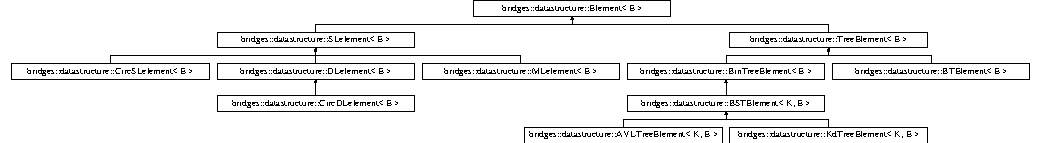
\includegraphics[height=1.917808cm]{classbridges_1_1datastructure_1_1_element}
\end{center}
\end{figure}


\subsection{Detailed Description}
\subsubsection*{template$<$typename E$>$\newline
class bridges\+::datastructure\+::\+Element$<$ E $>$}

This is the fundamental building block for all data structures in B\+R\+I\+D\+G\+ES. 

This is the Superclass \hyperlink{classbridges_1_1datastructure_1_1_element}{Element} with \hyperlink{classbridges_1_1datastructure_1_1_s_lelement}{S\+Lelement}, \hyperlink{classbridges_1_1datastructure_1_1_d_lelement}{D\+Lelement}, M\+L\+Element, Circ\+Sl\+Element, Circ\+Dl\+Element, \hyperlink{classbridges_1_1datastructure_1_1_tree_element}{Tree\+Element}, \hyperlink{classbridges_1_1datastructure_1_1_bin_tree_element}{Bin\+Tree\+Element}, \hyperlink{classbridges_1_1datastructure_1_1_b_s_t_element}{B\+S\+T\+Element}, \hyperlink{classbridges_1_1datastructure_1_1_a_v_l_tree_element}{A\+V\+L\+Tree\+Element}, \hyperlink{classbridges_1_1datastructure_1_1_kd_tree_element}{Kd\+Tree\+Element} subclasses.

The label field(string type) is used to label the visualization of the element.

\hyperlink{classbridges_1_1datastructure_1_1_element}{Element} holds a \hyperlink{classbridges_1_1datastructure_1_1_link_visualizer}{Link\+Visualizer} for each of its links and an \hyperlink{classbridges_1_1datastructure_1_1_element_visualizer}{Element\+Visualizer} for itself


\begin{DoxyParams}{Parameters}
{\em E} & the application data type\\
\hline
\end{DoxyParams}
\begin{DoxyAuthor}{Author}
Kalpathi Subramanian
\end{DoxyAuthor}
\begin{DoxyDate}{Date}
6/11/15, 11/27/16, 7/12/19 
\end{DoxyDate}
\subsection*{Public Member Functions}
\begin{DoxyCompactItemize}
\item 
\hyperlink{classbridges_1_1datastructure_1_1_element_a21820b1d88f2eb25adfe768bd03046d6}{Element} (const E \&val=E(), const string \&lab=string())
\item 
\hyperlink{classbridges_1_1datastructure_1_1_element_a80eb6ac6925c4974c2e88e7e1446e231}{Element} (const \hyperlink{classbridges_1_1datastructure_1_1_element}{Element} \&e)
\item 
\hyperlink{classbridges_1_1datastructure_1_1_element}{Element} \& \hyperlink{classbridges_1_1datastructure_1_1_element_a6446ad27ba42a854ff93b74b4d7eb3cb}{operator=} (const \hyperlink{classbridges_1_1datastructure_1_1_element}{Element} \&e)
\item 
E \& \hyperlink{classbridges_1_1datastructure_1_1_element_a18ffc753328275e95bb1ee967f88a00a}{operator=} (E const \&e)
\item 
virtual \hyperlink{classbridges_1_1datastructure_1_1_element_ad7ed60da8ed4a31b7a2678d0aa5db205}{$\sim$\+Element} ()
\item 
\hyperlink{classbridges_1_1datastructure_1_1_element_visualizer}{Element\+Visualizer} $\ast$ \hyperlink{classbridges_1_1datastructure_1_1_element_ad4f9ca479938bacd4586df8e7ede2116}{get\+Visualizer} ()
\item 
const \hyperlink{classbridges_1_1datastructure_1_1_element_visualizer}{Element\+Visualizer} $\ast$ \hyperlink{classbridges_1_1datastructure_1_1_element_a75a7770c3b6b1a6cd826293ea33d2d0a}{get\+Visualizer} () const
\item 
\hyperlink{classbridges_1_1datastructure_1_1_link_visualizer}{Link\+Visualizer} $\ast$ \hyperlink{classbridges_1_1datastructure_1_1_element_a531bde8ec32ef31b6d88af37cb029d86}{get\+Link\+Visualizer} (const \hyperlink{classbridges_1_1datastructure_1_1_element}{Element} $\ast$el)
\item 
\hyperlink{classbridges_1_1datastructure_1_1_link_visualizer}{Link\+Visualizer} $\ast$ \hyperlink{classbridges_1_1datastructure_1_1_element_a5e3b55d5098d72d4a83b68a60584a3a1}{get\+Link\+Visualizer} (const \hyperlink{classbridges_1_1datastructure_1_1_element}{Element} $\ast$el) const
\item 
string const  \& \hyperlink{classbridges_1_1datastructure_1_1_element_a44949edf79379a4d48490e98c15992a6}{get\+Label} () const
\item 
void \hyperlink{classbridges_1_1datastructure_1_1_element_a3a1fe4e3aa100125710c30f6e401e8c3}{set\+Label} (const string \&lab)
\item 
E const  \& \hyperlink{classbridges_1_1datastructure_1_1_element_acf6e068c6b00ff0d20ed42af32ff1f38}{get\+Value} () const
\item 
E \& \hyperlink{classbridges_1_1datastructure_1_1_element_abba0b4c03eb6fd08aed17eeb3be5bd1b}{get\+Value} ()
\item 
void \hyperlink{classbridges_1_1datastructure_1_1_element_a26f2aceb9eed7195fd55b3538f3c059f}{set\+Value} (const E \&val)
\item 
void \hyperlink{classbridges_1_1datastructure_1_1_element_a3200b0ac712c1720db62d1f0bbcb14be}{set\+Size} (const double \&sz)
\begin{DoxyCompactList}\small\item\em Sets size of the element. \end{DoxyCompactList}\item 
double \hyperlink{classbridges_1_1datastructure_1_1_element_a8c0b15450978b03c8ebf6a3c23092cba}{get\+Size} () const
\item 
void \hyperlink{classbridges_1_1datastructure_1_1_element_a17d75aae50a48b3404f3c6811c62ae1c}{set\+Color} (const \hyperlink{classbridges_1_1datastructure_1_1_color}{Color} \&col)
\begin{DoxyCompactList}\small\item\em Set the color of the \hyperlink{classbridges_1_1datastructure_1_1_element}{Element}. \end{DoxyCompactList}\item 
void \hyperlink{classbridges_1_1datastructure_1_1_element_a3792c8d514f4d644d739c6124f26bcbf}{set\+Color} (const string col)
\begin{DoxyCompactList}\small\item\em Set the color by name. \end{DoxyCompactList}\item 
\hyperlink{classbridges_1_1datastructure_1_1_color}{Color} \hyperlink{classbridges_1_1datastructure_1_1_element_adf441bce0ef9e4abd36c1df00ea5932c}{get\+Color} () const
\begin{DoxyCompactList}\small\item\em Get the current color of the element. \end{DoxyCompactList}\item 
void \hyperlink{classbridges_1_1datastructure_1_1_element_acb5d0b5734a6b3c17b7b1784ae1dc79c}{set\+Opacity} (double opacity)
\item 
double \hyperlink{classbridges_1_1datastructure_1_1_element_acf14bfc12da42565b237a7bd79bd36c2}{get\+Opacity} ()
\item 
void \hyperlink{classbridges_1_1datastructure_1_1_element_a1ef398bf1027244a624575e58a569ed9}{set\+Shape} (const \hyperlink{namespacebridges_1_1datastructure_a3408f5f44d9c6062e5f3adb7e1bbb7f0}{Shape} \&shp)
\begin{DoxyCompactList}\small\item\em Set the shape of the element. \end{DoxyCompactList}\item 
\hyperlink{namespacebridges_1_1datastructure_a3408f5f44d9c6062e5f3adb7e1bbb7f0}{Shape} \hyperlink{classbridges_1_1datastructure_1_1_element_acb8680aa406733d36411fd189017706c}{get\+Shape} () const
\begin{DoxyCompactList}\small\item\em Returns the shape of the element. \end{DoxyCompactList}\item 
void \hyperlink{classbridges_1_1datastructure_1_1_element_af3af017c9d6efcbc2124d0231b57e7a6}{set\+Location} (const double \&locX, const double \&locY)
\item 
double \hyperlink{classbridges_1_1datastructure_1_1_element_a471f2f69147deb0f514bb9720e0e18ea}{get\+LocationX} () const
\item 
double \hyperlink{classbridges_1_1datastructure_1_1_element_a6394039086bc1f27f2e6adf73294a74b}{get\+LocationY} () const
\end{DoxyCompactItemize}
\subsection*{Protected Member Functions}
\begin{DoxyCompactItemize}
\item 
virtual const string \hyperlink{classbridges_1_1datastructure_1_1_element_a285fc51d6dfcb8bff2d72f7e4addfe6d}{get\+Element\+Representation} () const
\end{DoxyCompactItemize}
\subsection*{Static Protected Member Functions}
\begin{DoxyCompactItemize}
\item 
static const string \hyperlink{classbridges_1_1datastructure_1_1_element_a0d43c0aaa96192b49dfc0a499d63a325}{get\+Link\+Representation} (const \hyperlink{classbridges_1_1datastructure_1_1_link_visualizer}{Link\+Visualizer} \&lv, const string \&src, const string \&dest)
\item 
static const string \hyperlink{classbridges_1_1datastructure_1_1_element_afc6de63b836064024721d72b7ffa52bf}{get\+C\+S\+S\+Representation} (const \hyperlink{classbridges_1_1datastructure_1_1_color}{Color} \&col)
\end{DoxyCompactItemize}
\subsection*{Protected Attributes}
\begin{DoxyCompactItemize}
\item 
unordered\+\_\+map$<$ \hyperlink{classbridges_1_1datastructure_1_1_element}{Element} $\ast$, \hyperlink{classbridges_1_1datastructure_1_1_link_visualizer}{Link\+Visualizer} $>$ \hyperlink{classbridges_1_1datastructure_1_1_element_ac296ae66e6b04e95f31f4134228524f8}{links}
\end{DoxyCompactItemize}
\subsection*{Friends}
\begin{DoxyCompactItemize}
\item 
{\footnotesize template$<$typename K , typename E1 , typename E2 $>$ }\\class \hyperlink{classbridges_1_1datastructure_1_1_element_a65850138f0763fec43a76fb942f0eccc}{Graph\+Adj\+List}
\item 
{\footnotesize template$<$typename K , typename E1 , typename E2 $>$ }\\class \hyperlink{classbridges_1_1datastructure_1_1_element_a1935808473b7eb8ff54149c5436c3ac9}{Graph\+Adj\+Matrix}
\item 
{\footnotesize template$<$typename K $>$ }\\class \hyperlink{classbridges_1_1datastructure_1_1_element_ab1a595168ea1870ce436dfd2d8e69b6d}{Array}
\item 
{\footnotesize template$<$typename K $>$ }\\class \hyperlink{classbridges_1_1datastructure_1_1_element_a71a2fa1cdcc1e193c1790c39b8267780}{Array1D}
\item 
{\footnotesize template$<$typename K $>$ }\\class \hyperlink{classbridges_1_1datastructure_1_1_element_a335c96c00a46d6b064b5af268ae03e42}{Array2D}
\item 
{\footnotesize template$<$typename K $>$ }\\class \hyperlink{classbridges_1_1datastructure_1_1_element_a2adb97d98cc3a6fe0cd1daaf40058938}{Array3D}
\end{DoxyCompactItemize}


\subsection{Constructor \& Destructor Documentation}
\mbox{\Hypertarget{classbridges_1_1datastructure_1_1_element_a21820b1d88f2eb25adfe768bd03046d6}\label{classbridges_1_1datastructure_1_1_element_a21820b1d88f2eb25adfe768bd03046d6}} 
\index{bridges\+::datastructure\+::\+Element@{bridges\+::datastructure\+::\+Element}!Element@{Element}}
\index{Element@{Element}!bridges\+::datastructure\+::\+Element@{bridges\+::datastructure\+::\+Element}}
\subsubsection{\texorpdfstring{Element()}{Element()}\hspace{0.1cm}{\footnotesize\ttfamily [1/2]}}
{\footnotesize\ttfamily template$<$typename E$>$ \\
\hyperlink{classbridges_1_1datastructure_1_1_element}{bridges\+::datastructure\+::\+Element}$<$ E $>$\+::\hyperlink{classbridges_1_1datastructure_1_1_element}{Element} (\begin{DoxyParamCaption}\item[{const E \&}]{val = {\ttfamily E()},  }\item[{const string \&}]{lab = {\ttfamily string()} }\end{DoxyParamCaption})\hspace{0.3cm}{\ttfamily [inline]}, {\ttfamily [explicit]}}

Constructs an element with the provided value and label. The defaults will be used if not provided.


\begin{DoxyParams}{Parameters}
{\em val} & The data to hold \\
\hline
{\em lab} & The label to show \\
\hline
\end{DoxyParams}
\mbox{\Hypertarget{classbridges_1_1datastructure_1_1_element_a80eb6ac6925c4974c2e88e7e1446e231}\label{classbridges_1_1datastructure_1_1_element_a80eb6ac6925c4974c2e88e7e1446e231}} 
\index{bridges\+::datastructure\+::\+Element@{bridges\+::datastructure\+::\+Element}!Element@{Element}}
\index{Element@{Element}!bridges\+::datastructure\+::\+Element@{bridges\+::datastructure\+::\+Element}}
\subsubsection{\texorpdfstring{Element()}{Element()}\hspace{0.1cm}{\footnotesize\ttfamily [2/2]}}
{\footnotesize\ttfamily template$<$typename E$>$ \\
\hyperlink{classbridges_1_1datastructure_1_1_element}{bridges\+::datastructure\+::\+Element}$<$ E $>$\+::\hyperlink{classbridges_1_1datastructure_1_1_element}{Element} (\begin{DoxyParamCaption}\item[{const \hyperlink{classbridges_1_1datastructure_1_1_element}{Element}$<$ E $>$ \&}]{e }\end{DoxyParamCaption})\hspace{0.3cm}{\ttfamily [inline]}}

Constructs an element with the provided element as input 
\begin{DoxyParams}{Parameters}
{\em e} & element \\
\hline
\end{DoxyParams}
\mbox{\Hypertarget{classbridges_1_1datastructure_1_1_element_ad7ed60da8ed4a31b7a2678d0aa5db205}\label{classbridges_1_1datastructure_1_1_element_ad7ed60da8ed4a31b7a2678d0aa5db205}} 
\index{bridges\+::datastructure\+::\+Element@{bridges\+::datastructure\+::\+Element}!````~Element@{$\sim$\+Element}}
\index{````~Element@{$\sim$\+Element}!bridges\+::datastructure\+::\+Element@{bridges\+::datastructure\+::\+Element}}
\subsubsection{\texorpdfstring{$\sim$\+Element()}{~Element()}}
{\footnotesize\ttfamily template$<$typename E$>$ \\
virtual \hyperlink{classbridges_1_1datastructure_1_1_element}{bridges\+::datastructure\+::\+Element}$<$ E $>$\+::$\sim$\hyperlink{classbridges_1_1datastructure_1_1_element}{Element} (\begin{DoxyParamCaption}{ }\end{DoxyParamCaption})\hspace{0.3cm}{\ttfamily [inline]}, {\ttfamily [virtual]}}

\hyperlink{classbridges_1_1datastructure_1_1_element}{Element} destructor 

\subsection{Member Function Documentation}
\mbox{\Hypertarget{classbridges_1_1datastructure_1_1_element_adf441bce0ef9e4abd36c1df00ea5932c}\label{classbridges_1_1datastructure_1_1_element_adf441bce0ef9e4abd36c1df00ea5932c}} 
\index{bridges\+::datastructure\+::\+Element@{bridges\+::datastructure\+::\+Element}!get\+Color@{get\+Color}}
\index{get\+Color@{get\+Color}!bridges\+::datastructure\+::\+Element@{bridges\+::datastructure\+::\+Element}}
\subsubsection{\texorpdfstring{get\+Color()}{getColor()}}
{\footnotesize\ttfamily template$<$typename E$>$ \\
\hyperlink{classbridges_1_1datastructure_1_1_color}{Color} \hyperlink{classbridges_1_1datastructure_1_1_element}{bridges\+::datastructure\+::\+Element}$<$ E $>$\+::get\+Color (\begin{DoxyParamCaption}{ }\end{DoxyParamCaption}) const\hspace{0.3cm}{\ttfamily [inline]}}



Get the current color of the element. 

\begin{DoxyReturn}{Returns}
The color of the element 
\end{DoxyReturn}
\mbox{\Hypertarget{classbridges_1_1datastructure_1_1_element_afc6de63b836064024721d72b7ffa52bf}\label{classbridges_1_1datastructure_1_1_element_afc6de63b836064024721d72b7ffa52bf}} 
\index{bridges\+::datastructure\+::\+Element@{bridges\+::datastructure\+::\+Element}!get\+C\+S\+S\+Representation@{get\+C\+S\+S\+Representation}}
\index{get\+C\+S\+S\+Representation@{get\+C\+S\+S\+Representation}!bridges\+::datastructure\+::\+Element@{bridges\+::datastructure\+::\+Element}}
\subsubsection{\texorpdfstring{get\+C\+S\+S\+Representation()}{getCSSRepresentation()}}
{\footnotesize\ttfamily template$<$typename E$>$ \\
static const string \hyperlink{classbridges_1_1datastructure_1_1_element}{bridges\+::datastructure\+::\+Element}$<$ E $>$\+::get\+C\+S\+S\+Representation (\begin{DoxyParamCaption}\item[{const \hyperlink{classbridges_1_1datastructure_1_1_color}{Color} \&}]{col }\end{DoxyParamCaption})\hspace{0.3cm}{\ttfamily [inline]}, {\ttfamily [static]}, {\ttfamily [protected]}}

Gets the J\+S\+ON representation of this color


\begin{DoxyParams}{Parameters}
{\em col} & The \hyperlink{classbridges_1_1datastructure_1_1_color}{Color} \\
\hline
\end{DoxyParams}
\begin{DoxyReturn}{Returns}
Equivilant Legal C\+SS color representation 
\end{DoxyReturn}
\mbox{\Hypertarget{classbridges_1_1datastructure_1_1_element_a285fc51d6dfcb8bff2d72f7e4addfe6d}\label{classbridges_1_1datastructure_1_1_element_a285fc51d6dfcb8bff2d72f7e4addfe6d}} 
\index{bridges\+::datastructure\+::\+Element@{bridges\+::datastructure\+::\+Element}!get\+Element\+Representation@{get\+Element\+Representation}}
\index{get\+Element\+Representation@{get\+Element\+Representation}!bridges\+::datastructure\+::\+Element@{bridges\+::datastructure\+::\+Element}}
\subsubsection{\texorpdfstring{get\+Element\+Representation()}{getElementRepresentation()}}
{\footnotesize\ttfamily template$<$typename E$>$ \\
virtual const string \hyperlink{classbridges_1_1datastructure_1_1_element}{bridges\+::datastructure\+::\+Element}$<$ E $>$\+::get\+Element\+Representation (\begin{DoxyParamCaption}{ }\end{DoxyParamCaption}) const\hspace{0.3cm}{\ttfamily [inline]}, {\ttfamily [protected]}, {\ttfamily [virtual]}}

Gets the J\+S\+ON string of the element representation \begin{DoxyReturn}{Returns}
The J\+S\+ON string of this element\textquotesingle{}s properties 
\end{DoxyReturn}


Reimplemented in \hyperlink{classbridges_1_1datastructure_1_1_kd_tree_element_a5413ecaf152e3df5fb45dd85da812888}{bridges\+::datastructure\+::\+Kd\+Tree\+Element$<$ K, E $>$}, and \hyperlink{classbridges_1_1datastructure_1_1_b_s_t_element_a8f962a01b6e0eff59abeee7768264fd9}{bridges\+::datastructure\+::\+B\+S\+T\+Element$<$ K, E $>$}.

\mbox{\Hypertarget{classbridges_1_1datastructure_1_1_element_a44949edf79379a4d48490e98c15992a6}\label{classbridges_1_1datastructure_1_1_element_a44949edf79379a4d48490e98c15992a6}} 
\index{bridges\+::datastructure\+::\+Element@{bridges\+::datastructure\+::\+Element}!get\+Label@{get\+Label}}
\index{get\+Label@{get\+Label}!bridges\+::datastructure\+::\+Element@{bridges\+::datastructure\+::\+Element}}
\subsubsection{\texorpdfstring{get\+Label()}{getLabel()}}
{\footnotesize\ttfamily template$<$typename E$>$ \\
string const\& \hyperlink{classbridges_1_1datastructure_1_1_element}{bridges\+::datastructure\+::\+Element}$<$ E $>$\+::get\+Label (\begin{DoxyParamCaption}{ }\end{DoxyParamCaption}) const\hspace{0.3cm}{\ttfamily [inline]}}

Gets the label of this element \begin{DoxyReturn}{Returns}
The label of the element 
\end{DoxyReturn}
\mbox{\Hypertarget{classbridges_1_1datastructure_1_1_element_a0d43c0aaa96192b49dfc0a499d63a325}\label{classbridges_1_1datastructure_1_1_element_a0d43c0aaa96192b49dfc0a499d63a325}} 
\index{bridges\+::datastructure\+::\+Element@{bridges\+::datastructure\+::\+Element}!get\+Link\+Representation@{get\+Link\+Representation}}
\index{get\+Link\+Representation@{get\+Link\+Representation}!bridges\+::datastructure\+::\+Element@{bridges\+::datastructure\+::\+Element}}
\subsubsection{\texorpdfstring{get\+Link\+Representation()}{getLinkRepresentation()}}
{\footnotesize\ttfamily template$<$typename E$>$ \\
static const string \hyperlink{classbridges_1_1datastructure_1_1_element}{bridges\+::datastructure\+::\+Element}$<$ E $>$\+::get\+Link\+Representation (\begin{DoxyParamCaption}\item[{const \hyperlink{classbridges_1_1datastructure_1_1_link_visualizer}{Link\+Visualizer} \&}]{lv,  }\item[{const string \&}]{src,  }\item[{const string \&}]{dest }\end{DoxyParamCaption})\hspace{0.3cm}{\ttfamily [inline]}, {\ttfamily [static]}, {\ttfamily [protected]}}

Gets the J\+S\+ON representation of this link visualizer using the supplied source and destination strings


\begin{DoxyParams}{Parameters}
{\em lv} & The \hyperlink{classbridges_1_1datastructure_1_1_link_visualizer}{Link\+Visualizer} \\
\hline
{\em src} & The source vertex \\
\hline
{\em dest} & The destination vertex \\
\hline
\end{DoxyParams}
\begin{DoxyReturn}{Returns}
The J\+S\+ON of this link visualizer 
\end{DoxyReturn}
\mbox{\Hypertarget{classbridges_1_1datastructure_1_1_element_a531bde8ec32ef31b6d88af37cb029d86}\label{classbridges_1_1datastructure_1_1_element_a531bde8ec32ef31b6d88af37cb029d86}} 
\index{bridges\+::datastructure\+::\+Element@{bridges\+::datastructure\+::\+Element}!get\+Link\+Visualizer@{get\+Link\+Visualizer}}
\index{get\+Link\+Visualizer@{get\+Link\+Visualizer}!bridges\+::datastructure\+::\+Element@{bridges\+::datastructure\+::\+Element}}
\subsubsection{\texorpdfstring{get\+Link\+Visualizer()}{getLinkVisualizer()}\hspace{0.1cm}{\footnotesize\ttfamily [1/2]}}
{\footnotesize\ttfamily template$<$typename E$>$ \\
\hyperlink{classbridges_1_1datastructure_1_1_link_visualizer}{Link\+Visualizer}$\ast$ \hyperlink{classbridges_1_1datastructure_1_1_element}{bridges\+::datastructure\+::\+Element}$<$ E $>$\+::get\+Link\+Visualizer (\begin{DoxyParamCaption}\item[{const \hyperlink{classbridges_1_1datastructure_1_1_element}{Element}$<$ E $>$ $\ast$}]{el }\end{DoxyParamCaption})\hspace{0.3cm}{\ttfamily [inline]}}

Returns the \hyperlink{classbridges_1_1datastructure_1_1_link_visualizer}{Link\+Visualizer} of element \char`\"{}el\char`\"{} or N\+U\+LL if no link exists


\begin{DoxyParams}{Parameters}
{\em el} & The terminating element of the link\\
\hline
\end{DoxyParams}
\begin{DoxyReturn}{Returns}
The \hyperlink{classbridges_1_1datastructure_1_1_link_visualizer}{Link\+Visualizer} 
\end{DoxyReturn}
\mbox{\Hypertarget{classbridges_1_1datastructure_1_1_element_a5e3b55d5098d72d4a83b68a60584a3a1}\label{classbridges_1_1datastructure_1_1_element_a5e3b55d5098d72d4a83b68a60584a3a1}} 
\index{bridges\+::datastructure\+::\+Element@{bridges\+::datastructure\+::\+Element}!get\+Link\+Visualizer@{get\+Link\+Visualizer}}
\index{get\+Link\+Visualizer@{get\+Link\+Visualizer}!bridges\+::datastructure\+::\+Element@{bridges\+::datastructure\+::\+Element}}
\subsubsection{\texorpdfstring{get\+Link\+Visualizer()}{getLinkVisualizer()}\hspace{0.1cm}{\footnotesize\ttfamily [2/2]}}
{\footnotesize\ttfamily template$<$typename E$>$ \\
\hyperlink{classbridges_1_1datastructure_1_1_link_visualizer}{Link\+Visualizer}$\ast$ \hyperlink{classbridges_1_1datastructure_1_1_element}{bridges\+::datastructure\+::\+Element}$<$ E $>$\+::get\+Link\+Visualizer (\begin{DoxyParamCaption}\item[{const \hyperlink{classbridges_1_1datastructure_1_1_element}{Element}$<$ E $>$ $\ast$}]{el }\end{DoxyParamCaption}) const\hspace{0.3cm}{\ttfamily [inline]}}

Returns the \hyperlink{classbridges_1_1datastructure_1_1_link_visualizer}{Link\+Visualizer} of element \char`\"{}el\char`\"{} -\/ Constant version


\begin{DoxyParams}{Parameters}
{\em el} & The terminating element of the link \\
\hline
\end{DoxyParams}
\begin{DoxyReturn}{Returns}
The \hyperlink{classbridges_1_1datastructure_1_1_link_visualizer}{Link\+Visualizer} 
\end{DoxyReturn}
\mbox{\Hypertarget{classbridges_1_1datastructure_1_1_element_a471f2f69147deb0f514bb9720e0e18ea}\label{classbridges_1_1datastructure_1_1_element_a471f2f69147deb0f514bb9720e0e18ea}} 
\index{bridges\+::datastructure\+::\+Element@{bridges\+::datastructure\+::\+Element}!get\+LocationX@{get\+LocationX}}
\index{get\+LocationX@{get\+LocationX}!bridges\+::datastructure\+::\+Element@{bridges\+::datastructure\+::\+Element}}
\subsubsection{\texorpdfstring{get\+Location\+X()}{getLocationX()}}
{\footnotesize\ttfamily template$<$typename E$>$ \\
double \hyperlink{classbridges_1_1datastructure_1_1_element}{bridges\+::datastructure\+::\+Element}$<$ E $>$\+::get\+LocationX (\begin{DoxyParamCaption}{ }\end{DoxyParamCaption}) const\hspace{0.3cm}{\ttfamily [inline]}}

Gets the X coordinate of the location \begin{DoxyReturn}{Returns}
the X coordinate of the element\textquotesingle{}s location attribute 
\end{DoxyReturn}
\mbox{\Hypertarget{classbridges_1_1datastructure_1_1_element_a6394039086bc1f27f2e6adf73294a74b}\label{classbridges_1_1datastructure_1_1_element_a6394039086bc1f27f2e6adf73294a74b}} 
\index{bridges\+::datastructure\+::\+Element@{bridges\+::datastructure\+::\+Element}!get\+LocationY@{get\+LocationY}}
\index{get\+LocationY@{get\+LocationY}!bridges\+::datastructure\+::\+Element@{bridges\+::datastructure\+::\+Element}}
\subsubsection{\texorpdfstring{get\+Location\+Y()}{getLocationY()}}
{\footnotesize\ttfamily template$<$typename E$>$ \\
double \hyperlink{classbridges_1_1datastructure_1_1_element}{bridges\+::datastructure\+::\+Element}$<$ E $>$\+::get\+LocationY (\begin{DoxyParamCaption}{ }\end{DoxyParamCaption}) const\hspace{0.3cm}{\ttfamily [inline]}}

Gets the Y coordinate of the location \begin{DoxyReturn}{Returns}
the Y coordinate of the element\textquotesingle{}s location attribute 
\end{DoxyReturn}
\mbox{\Hypertarget{classbridges_1_1datastructure_1_1_element_acf14bfc12da42565b237a7bd79bd36c2}\label{classbridges_1_1datastructure_1_1_element_acf14bfc12da42565b237a7bd79bd36c2}} 
\index{bridges\+::datastructure\+::\+Element@{bridges\+::datastructure\+::\+Element}!get\+Opacity@{get\+Opacity}}
\index{get\+Opacity@{get\+Opacity}!bridges\+::datastructure\+::\+Element@{bridges\+::datastructure\+::\+Element}}
\subsubsection{\texorpdfstring{get\+Opacity()}{getOpacity()}}
{\footnotesize\ttfamily template$<$typename E$>$ \\
double \hyperlink{classbridges_1_1datastructure_1_1_element}{bridges\+::datastructure\+::\+Element}$<$ E $>$\+::get\+Opacity (\begin{DoxyParamCaption}{ }\end{DoxyParamCaption})\hspace{0.3cm}{\ttfamily [inline]}}

get opacity of element

\begin{DoxyReturn}{Returns}
opacity 
\end{DoxyReturn}
\mbox{\Hypertarget{classbridges_1_1datastructure_1_1_element_acb8680aa406733d36411fd189017706c}\label{classbridges_1_1datastructure_1_1_element_acb8680aa406733d36411fd189017706c}} 
\index{bridges\+::datastructure\+::\+Element@{bridges\+::datastructure\+::\+Element}!get\+Shape@{get\+Shape}}
\index{get\+Shape@{get\+Shape}!bridges\+::datastructure\+::\+Element@{bridges\+::datastructure\+::\+Element}}
\subsubsection{\texorpdfstring{get\+Shape()}{getShape()}}
{\footnotesize\ttfamily template$<$typename E$>$ \\
\hyperlink{namespacebridges_1_1datastructure_a3408f5f44d9c6062e5f3adb7e1bbb7f0}{Shape} \hyperlink{classbridges_1_1datastructure_1_1_element}{bridges\+::datastructure\+::\+Element}$<$ E $>$\+::get\+Shape (\begin{DoxyParamCaption}{ }\end{DoxyParamCaption}) const\hspace{0.3cm}{\ttfamily [inline]}}



Returns the shape of the element. 

\begin{DoxyReturn}{Returns}
The shape of the element(one of Shape.\+C\+I\+R\+C\+LE, Shape.\+S\+Q\+U\+A\+RE, Shape.\+D\+I\+A\+M\+O\+ND, Shape.\+C\+R\+O\+SS, Shape.\+T\+R\+I\+A\+N\+G\+LE, Shape.\+W\+YE, Shape.\+S\+T\+AR) 
\end{DoxyReturn}
\mbox{\Hypertarget{classbridges_1_1datastructure_1_1_element_a8c0b15450978b03c8ebf6a3c23092cba}\label{classbridges_1_1datastructure_1_1_element_a8c0b15450978b03c8ebf6a3c23092cba}} 
\index{bridges\+::datastructure\+::\+Element@{bridges\+::datastructure\+::\+Element}!get\+Size@{get\+Size}}
\index{get\+Size@{get\+Size}!bridges\+::datastructure\+::\+Element@{bridges\+::datastructure\+::\+Element}}
\subsubsection{\texorpdfstring{get\+Size()}{getSize()}}
{\footnotesize\ttfamily template$<$typename E$>$ \\
double \hyperlink{classbridges_1_1datastructure_1_1_element}{bridges\+::datastructure\+::\+Element}$<$ E $>$\+::get\+Size (\begin{DoxyParamCaption}{ }\end{DoxyParamCaption}) const\hspace{0.3cm}{\ttfamily [inline]}}

Get element size \begin{DoxyReturn}{Returns}
the size (in pixels) of the element 
\end{DoxyReturn}
\mbox{\Hypertarget{classbridges_1_1datastructure_1_1_element_acf6e068c6b00ff0d20ed42af32ff1f38}\label{classbridges_1_1datastructure_1_1_element_acf6e068c6b00ff0d20ed42af32ff1f38}} 
\index{bridges\+::datastructure\+::\+Element@{bridges\+::datastructure\+::\+Element}!get\+Value@{get\+Value}}
\index{get\+Value@{get\+Value}!bridges\+::datastructure\+::\+Element@{bridges\+::datastructure\+::\+Element}}
\subsubsection{\texorpdfstring{get\+Value()}{getValue()}\hspace{0.1cm}{\footnotesize\ttfamily [1/2]}}
{\footnotesize\ttfamily template$<$typename E$>$ \\
E const\& \hyperlink{classbridges_1_1datastructure_1_1_element}{bridges\+::datastructure\+::\+Element}$<$ E $>$\+::get\+Value (\begin{DoxyParamCaption}{ }\end{DoxyParamCaption}) const\hspace{0.3cm}{\ttfamily [inline]}}

Gets the object (generic) held in the element -\/ const version \begin{DoxyReturn}{Returns}
The value of the element 
\end{DoxyReturn}
\mbox{\Hypertarget{classbridges_1_1datastructure_1_1_element_abba0b4c03eb6fd08aed17eeb3be5bd1b}\label{classbridges_1_1datastructure_1_1_element_abba0b4c03eb6fd08aed17eeb3be5bd1b}} 
\index{bridges\+::datastructure\+::\+Element@{bridges\+::datastructure\+::\+Element}!get\+Value@{get\+Value}}
\index{get\+Value@{get\+Value}!bridges\+::datastructure\+::\+Element@{bridges\+::datastructure\+::\+Element}}
\subsubsection{\texorpdfstring{get\+Value()}{getValue()}\hspace{0.1cm}{\footnotesize\ttfamily [2/2]}}
{\footnotesize\ttfamily template$<$typename E$>$ \\
E\& \hyperlink{classbridges_1_1datastructure_1_1_element}{bridges\+::datastructure\+::\+Element}$<$ E $>$\+::get\+Value (\begin{DoxyParamCaption}{ }\end{DoxyParamCaption})\hspace{0.3cm}{\ttfamily [inline]}}

Gets the object (generic) held in the element \begin{DoxyReturn}{Returns}
The value of the element 
\end{DoxyReturn}
\mbox{\Hypertarget{classbridges_1_1datastructure_1_1_element_ad4f9ca479938bacd4586df8e7ede2116}\label{classbridges_1_1datastructure_1_1_element_ad4f9ca479938bacd4586df8e7ede2116}} 
\index{bridges\+::datastructure\+::\+Element@{bridges\+::datastructure\+::\+Element}!get\+Visualizer@{get\+Visualizer}}
\index{get\+Visualizer@{get\+Visualizer}!bridges\+::datastructure\+::\+Element@{bridges\+::datastructure\+::\+Element}}
\subsubsection{\texorpdfstring{get\+Visualizer()}{getVisualizer()}\hspace{0.1cm}{\footnotesize\ttfamily [1/2]}}
{\footnotesize\ttfamily template$<$typename E$>$ \\
\hyperlink{classbridges_1_1datastructure_1_1_element_visualizer}{Element\+Visualizer}$\ast$ \hyperlink{classbridges_1_1datastructure_1_1_element}{bridges\+::datastructure\+::\+Element}$<$ E $>$\+::get\+Visualizer (\begin{DoxyParamCaption}{ }\end{DoxyParamCaption})\hspace{0.3cm}{\ttfamily [inline]}}

Get the element visualizer object \begin{DoxyReturn}{Returns}
The \hyperlink{classbridges_1_1datastructure_1_1_element_visualizer}{Element\+Visualizer} of this element 
\end{DoxyReturn}
\mbox{\Hypertarget{classbridges_1_1datastructure_1_1_element_a75a7770c3b6b1a6cd826293ea33d2d0a}\label{classbridges_1_1datastructure_1_1_element_a75a7770c3b6b1a6cd826293ea33d2d0a}} 
\index{bridges\+::datastructure\+::\+Element@{bridges\+::datastructure\+::\+Element}!get\+Visualizer@{get\+Visualizer}}
\index{get\+Visualizer@{get\+Visualizer}!bridges\+::datastructure\+::\+Element@{bridges\+::datastructure\+::\+Element}}
\subsubsection{\texorpdfstring{get\+Visualizer()}{getVisualizer()}\hspace{0.1cm}{\footnotesize\ttfamily [2/2]}}
{\footnotesize\ttfamily template$<$typename E$>$ \\
const \hyperlink{classbridges_1_1datastructure_1_1_element_visualizer}{Element\+Visualizer}$\ast$ \hyperlink{classbridges_1_1datastructure_1_1_element}{bridges\+::datastructure\+::\+Element}$<$ E $>$\+::get\+Visualizer (\begin{DoxyParamCaption}{ }\end{DoxyParamCaption}) const\hspace{0.3cm}{\ttfamily [inline]}}

Get the element visualizer object -\/ constant version

\begin{DoxyReturn}{Returns}
The \hyperlink{classbridges_1_1datastructure_1_1_element_visualizer}{Element\+Visualizer} of this element 
\end{DoxyReturn}
\mbox{\Hypertarget{classbridges_1_1datastructure_1_1_element_a6446ad27ba42a854ff93b74b4d7eb3cb}\label{classbridges_1_1datastructure_1_1_element_a6446ad27ba42a854ff93b74b4d7eb3cb}} 
\index{bridges\+::datastructure\+::\+Element@{bridges\+::datastructure\+::\+Element}!operator=@{operator=}}
\index{operator=@{operator=}!bridges\+::datastructure\+::\+Element@{bridges\+::datastructure\+::\+Element}}
\subsubsection{\texorpdfstring{operator=()}{operator=()}\hspace{0.1cm}{\footnotesize\ttfamily [1/2]}}
{\footnotesize\ttfamily template$<$typename E$>$ \\
\hyperlink{classbridges_1_1datastructure_1_1_element}{Element}\& \hyperlink{classbridges_1_1datastructure_1_1_element}{bridges\+::datastructure\+::\+Element}$<$ E $>$\+::operator= (\begin{DoxyParamCaption}\item[{const \hyperlink{classbridges_1_1datastructure_1_1_element}{Element}$<$ E $>$ \&}]{e }\end{DoxyParamCaption})\hspace{0.3cm}{\ttfamily [inline]}}

\mbox{\Hypertarget{classbridges_1_1datastructure_1_1_element_a18ffc753328275e95bb1ee967f88a00a}\label{classbridges_1_1datastructure_1_1_element_a18ffc753328275e95bb1ee967f88a00a}} 
\index{bridges\+::datastructure\+::\+Element@{bridges\+::datastructure\+::\+Element}!operator=@{operator=}}
\index{operator=@{operator=}!bridges\+::datastructure\+::\+Element@{bridges\+::datastructure\+::\+Element}}
\subsubsection{\texorpdfstring{operator=()}{operator=()}\hspace{0.1cm}{\footnotesize\ttfamily [2/2]}}
{\footnotesize\ttfamily template$<$typename E$>$ \\
E\& \hyperlink{classbridges_1_1datastructure_1_1_element}{bridges\+::datastructure\+::\+Element}$<$ E $>$\+::operator= (\begin{DoxyParamCaption}\item[{E const \&}]{e }\end{DoxyParamCaption})\hspace{0.3cm}{\ttfamily [inline]}}

\mbox{\Hypertarget{classbridges_1_1datastructure_1_1_element_a17d75aae50a48b3404f3c6811c62ae1c}\label{classbridges_1_1datastructure_1_1_element_a17d75aae50a48b3404f3c6811c62ae1c}} 
\index{bridges\+::datastructure\+::\+Element@{bridges\+::datastructure\+::\+Element}!set\+Color@{set\+Color}}
\index{set\+Color@{set\+Color}!bridges\+::datastructure\+::\+Element@{bridges\+::datastructure\+::\+Element}}
\subsubsection{\texorpdfstring{set\+Color()}{setColor()}\hspace{0.1cm}{\footnotesize\ttfamily [1/2]}}
{\footnotesize\ttfamily template$<$typename E$>$ \\
void \hyperlink{classbridges_1_1datastructure_1_1_element}{bridges\+::datastructure\+::\+Element}$<$ E $>$\+::set\+Color (\begin{DoxyParamCaption}\item[{const \hyperlink{classbridges_1_1datastructure_1_1_color}{Color} \&}]{col }\end{DoxyParamCaption})\hspace{0.3cm}{\ttfamily [inline]}}



Set the color of the \hyperlink{classbridges_1_1datastructure_1_1_element}{Element}. 


\begin{DoxyParams}{Parameters}
{\em col} & The color of the element \\
\hline
\end{DoxyParams}
\mbox{\Hypertarget{classbridges_1_1datastructure_1_1_element_a3792c8d514f4d644d739c6124f26bcbf}\label{classbridges_1_1datastructure_1_1_element_a3792c8d514f4d644d739c6124f26bcbf}} 
\index{bridges\+::datastructure\+::\+Element@{bridges\+::datastructure\+::\+Element}!set\+Color@{set\+Color}}
\index{set\+Color@{set\+Color}!bridges\+::datastructure\+::\+Element@{bridges\+::datastructure\+::\+Element}}
\subsubsection{\texorpdfstring{set\+Color()}{setColor()}\hspace{0.1cm}{\footnotesize\ttfamily [2/2]}}
{\footnotesize\ttfamily template$<$typename E$>$ \\
void \hyperlink{classbridges_1_1datastructure_1_1_element}{bridges\+::datastructure\+::\+Element}$<$ E $>$\+::set\+Color (\begin{DoxyParamCaption}\item[{const string}]{col }\end{DoxyParamCaption})\hspace{0.3cm}{\ttfamily [inline]}}



Set the color by name. 


\begin{DoxyParams}{Parameters}
{\em col} & The color name. Refer to the \hyperlink{classbridges_1_1datastructure_1_1_color}{Color} class for supported color names. \\
\hline
\end{DoxyParams}
\mbox{\Hypertarget{classbridges_1_1datastructure_1_1_element_a3a1fe4e3aa100125710c30f6e401e8c3}\label{classbridges_1_1datastructure_1_1_element_a3a1fe4e3aa100125710c30f6e401e8c3}} 
\index{bridges\+::datastructure\+::\+Element@{bridges\+::datastructure\+::\+Element}!set\+Label@{set\+Label}}
\index{set\+Label@{set\+Label}!bridges\+::datastructure\+::\+Element@{bridges\+::datastructure\+::\+Element}}
\subsubsection{\texorpdfstring{set\+Label()}{setLabel()}}
{\footnotesize\ttfamily template$<$typename E$>$ \\
void \hyperlink{classbridges_1_1datastructure_1_1_element}{bridges\+::datastructure\+::\+Element}$<$ E $>$\+::set\+Label (\begin{DoxyParamCaption}\item[{const string \&}]{lab }\end{DoxyParamCaption})\hspace{0.3cm}{\ttfamily [inline]}}

Sets label of this element


\begin{DoxyParams}{Parameters}
{\em lab} & The label of the element \\
\hline
\end{DoxyParams}
\mbox{\Hypertarget{classbridges_1_1datastructure_1_1_element_af3af017c9d6efcbc2124d0231b57e7a6}\label{classbridges_1_1datastructure_1_1_element_af3af017c9d6efcbc2124d0231b57e7a6}} 
\index{bridges\+::datastructure\+::\+Element@{bridges\+::datastructure\+::\+Element}!set\+Location@{set\+Location}}
\index{set\+Location@{set\+Location}!bridges\+::datastructure\+::\+Element@{bridges\+::datastructure\+::\+Element}}
\subsubsection{\texorpdfstring{set\+Location()}{setLocation()}}
{\footnotesize\ttfamily template$<$typename E$>$ \\
void \hyperlink{classbridges_1_1datastructure_1_1_element}{bridges\+::datastructure\+::\+Element}$<$ E $>$\+::set\+Location (\begin{DoxyParamCaption}\item[{const double \&}]{locX,  }\item[{const double \&}]{locY }\end{DoxyParamCaption})\hspace{0.3cm}{\ttfamily [inline]}}

Sets the location attributes of an element.


\begin{DoxyParams}{Parameters}
{\em locX} & X coordinate of the element location \\
\hline
{\em locY} & Y coordinate of the element location \\
\hline
\end{DoxyParams}
\mbox{\Hypertarget{classbridges_1_1datastructure_1_1_element_acb5d0b5734a6b3c17b7b1784ae1dc79c}\label{classbridges_1_1datastructure_1_1_element_acb5d0b5734a6b3c17b7b1784ae1dc79c}} 
\index{bridges\+::datastructure\+::\+Element@{bridges\+::datastructure\+::\+Element}!set\+Opacity@{set\+Opacity}}
\index{set\+Opacity@{set\+Opacity}!bridges\+::datastructure\+::\+Element@{bridges\+::datastructure\+::\+Element}}
\subsubsection{\texorpdfstring{set\+Opacity()}{setOpacity()}}
{\footnotesize\ttfamily template$<$typename E$>$ \\
void \hyperlink{classbridges_1_1datastructure_1_1_element}{bridges\+::datastructure\+::\+Element}$<$ E $>$\+::set\+Opacity (\begin{DoxyParamCaption}\item[{double}]{opacity }\end{DoxyParamCaption})\hspace{0.3cm}{\ttfamily [inline]}}

set opacity of element -\/ use the 4th color component


\begin{DoxyParams}{Parameters}
{\em opacity} & \\
\hline
\end{DoxyParams}
\mbox{\Hypertarget{classbridges_1_1datastructure_1_1_element_a1ef398bf1027244a624575e58a569ed9}\label{classbridges_1_1datastructure_1_1_element_a1ef398bf1027244a624575e58a569ed9}} 
\index{bridges\+::datastructure\+::\+Element@{bridges\+::datastructure\+::\+Element}!set\+Shape@{set\+Shape}}
\index{set\+Shape@{set\+Shape}!bridges\+::datastructure\+::\+Element@{bridges\+::datastructure\+::\+Element}}
\subsubsection{\texorpdfstring{set\+Shape()}{setShape()}}
{\footnotesize\ttfamily template$<$typename E$>$ \\
void \hyperlink{classbridges_1_1datastructure_1_1_element}{bridges\+::datastructure\+::\+Element}$<$ E $>$\+::set\+Shape (\begin{DoxyParamCaption}\item[{const \hyperlink{namespacebridges_1_1datastructure_a3408f5f44d9c6062e5f3adb7e1bbb7f0}{Shape} \&}]{shp }\end{DoxyParamCaption})\hspace{0.3cm}{\ttfamily [inline]}}



Set the shape of the element. 


\begin{DoxyParams}{Parameters}
{\em shp} & is one of Shape.\+C\+I\+R\+C\+LE, Shape.\+S\+Q\+U\+A\+RE, Shape.\+D\+I\+A\+M\+O\+ND, Shape.\+C\+R\+O\+SS, Shape.\+T\+R\+I\+A\+N\+G\+LE, Shape.\+W\+YE, Shape.\+S\+T\+AR \\
\hline
\end{DoxyParams}
\mbox{\Hypertarget{classbridges_1_1datastructure_1_1_element_a3200b0ac712c1720db62d1f0bbcb14be}\label{classbridges_1_1datastructure_1_1_element_a3200b0ac712c1720db62d1f0bbcb14be}} 
\index{bridges\+::datastructure\+::\+Element@{bridges\+::datastructure\+::\+Element}!set\+Size@{set\+Size}}
\index{set\+Size@{set\+Size}!bridges\+::datastructure\+::\+Element@{bridges\+::datastructure\+::\+Element}}
\subsubsection{\texorpdfstring{set\+Size()}{setSize()}}
{\footnotesize\ttfamily template$<$typename E$>$ \\
void \hyperlink{classbridges_1_1datastructure_1_1_element}{bridges\+::datastructure\+::\+Element}$<$ E $>$\+::set\+Size (\begin{DoxyParamCaption}\item[{const double \&}]{sz }\end{DoxyParamCaption})\hspace{0.3cm}{\ttfamily [inline]}}



Sets size of the element. 


\begin{DoxyParams}{Parameters}
{\em sz} & The size in pixel weight of the element. Valid Range\+:\mbox{[}1;50\mbox{]} \\
\hline
\end{DoxyParams}
\mbox{\Hypertarget{classbridges_1_1datastructure_1_1_element_a26f2aceb9eed7195fd55b3538f3c059f}\label{classbridges_1_1datastructure_1_1_element_a26f2aceb9eed7195fd55b3538f3c059f}} 
\index{bridges\+::datastructure\+::\+Element@{bridges\+::datastructure\+::\+Element}!set\+Value@{set\+Value}}
\index{set\+Value@{set\+Value}!bridges\+::datastructure\+::\+Element@{bridges\+::datastructure\+::\+Element}}
\subsubsection{\texorpdfstring{set\+Value()}{setValue()}}
{\footnotesize\ttfamily template$<$typename E$>$ \\
void \hyperlink{classbridges_1_1datastructure_1_1_element}{bridges\+::datastructure\+::\+Element}$<$ E $>$\+::set\+Value (\begin{DoxyParamCaption}\item[{const E \&}]{val }\end{DoxyParamCaption})\hspace{0.3cm}{\ttfamily [inline]}}

Sets generic object to \char`\"{}val\char`\"{}


\begin{DoxyParams}{Parameters}
{\em val} & The value of the element to be set \\
\hline
\end{DoxyParams}


\subsection{Friends And Related Function Documentation}
\mbox{\Hypertarget{classbridges_1_1datastructure_1_1_element_ab1a595168ea1870ce436dfd2d8e69b6d}\label{classbridges_1_1datastructure_1_1_element_ab1a595168ea1870ce436dfd2d8e69b6d}} 
\index{bridges\+::datastructure\+::\+Element@{bridges\+::datastructure\+::\+Element}!Array@{Array}}
\index{Array@{Array}!bridges\+::datastructure\+::\+Element@{bridges\+::datastructure\+::\+Element}}
\subsubsection{\texorpdfstring{Array}{Array}}
{\footnotesize\ttfamily template$<$typename E$>$ \\
template$<$typename K $>$ \\
friend class \hyperlink{classbridges_1_1datastructure_1_1_array}{Array}\hspace{0.3cm}{\ttfamily [friend]}}

\mbox{\Hypertarget{classbridges_1_1datastructure_1_1_element_a71a2fa1cdcc1e193c1790c39b8267780}\label{classbridges_1_1datastructure_1_1_element_a71a2fa1cdcc1e193c1790c39b8267780}} 
\index{bridges\+::datastructure\+::\+Element@{bridges\+::datastructure\+::\+Element}!Array1D@{Array1D}}
\index{Array1D@{Array1D}!bridges\+::datastructure\+::\+Element@{bridges\+::datastructure\+::\+Element}}
\subsubsection{\texorpdfstring{Array1D}{Array1D}}
{\footnotesize\ttfamily template$<$typename E$>$ \\
template$<$typename K $>$ \\
friend class \hyperlink{classbridges_1_1datastructure_1_1_array1_d}{Array1D}\hspace{0.3cm}{\ttfamily [friend]}}

\mbox{\Hypertarget{classbridges_1_1datastructure_1_1_element_a335c96c00a46d6b064b5af268ae03e42}\label{classbridges_1_1datastructure_1_1_element_a335c96c00a46d6b064b5af268ae03e42}} 
\index{bridges\+::datastructure\+::\+Element@{bridges\+::datastructure\+::\+Element}!Array2D@{Array2D}}
\index{Array2D@{Array2D}!bridges\+::datastructure\+::\+Element@{bridges\+::datastructure\+::\+Element}}
\subsubsection{\texorpdfstring{Array2D}{Array2D}}
{\footnotesize\ttfamily template$<$typename E$>$ \\
template$<$typename K $>$ \\
friend class \hyperlink{classbridges_1_1datastructure_1_1_array2_d}{Array2D}\hspace{0.3cm}{\ttfamily [friend]}}

\mbox{\Hypertarget{classbridges_1_1datastructure_1_1_element_a2adb97d98cc3a6fe0cd1daaf40058938}\label{classbridges_1_1datastructure_1_1_element_a2adb97d98cc3a6fe0cd1daaf40058938}} 
\index{bridges\+::datastructure\+::\+Element@{bridges\+::datastructure\+::\+Element}!Array3D@{Array3D}}
\index{Array3D@{Array3D}!bridges\+::datastructure\+::\+Element@{bridges\+::datastructure\+::\+Element}}
\subsubsection{\texorpdfstring{Array3D}{Array3D}}
{\footnotesize\ttfamily template$<$typename E$>$ \\
template$<$typename K $>$ \\
friend class \hyperlink{classbridges_1_1datastructure_1_1_array3_d}{Array3D}\hspace{0.3cm}{\ttfamily [friend]}}

\mbox{\Hypertarget{classbridges_1_1datastructure_1_1_element_a65850138f0763fec43a76fb942f0eccc}\label{classbridges_1_1datastructure_1_1_element_a65850138f0763fec43a76fb942f0eccc}} 
\index{bridges\+::datastructure\+::\+Element@{bridges\+::datastructure\+::\+Element}!Graph\+Adj\+List@{Graph\+Adj\+List}}
\index{Graph\+Adj\+List@{Graph\+Adj\+List}!bridges\+::datastructure\+::\+Element@{bridges\+::datastructure\+::\+Element}}
\subsubsection{\texorpdfstring{Graph\+Adj\+List}{GraphAdjList}}
{\footnotesize\ttfamily template$<$typename E$>$ \\
template$<$typename K , typename E1 , typename E2 $>$ \\
friend class \hyperlink{classbridges_1_1datastructure_1_1_graph_adj_list}{Graph\+Adj\+List}\hspace{0.3cm}{\ttfamily [friend]}}

\mbox{\Hypertarget{classbridges_1_1datastructure_1_1_element_a1935808473b7eb8ff54149c5436c3ac9}\label{classbridges_1_1datastructure_1_1_element_a1935808473b7eb8ff54149c5436c3ac9}} 
\index{bridges\+::datastructure\+::\+Element@{bridges\+::datastructure\+::\+Element}!Graph\+Adj\+Matrix@{Graph\+Adj\+Matrix}}
\index{Graph\+Adj\+Matrix@{Graph\+Adj\+Matrix}!bridges\+::datastructure\+::\+Element@{bridges\+::datastructure\+::\+Element}}
\subsubsection{\texorpdfstring{Graph\+Adj\+Matrix}{GraphAdjMatrix}}
{\footnotesize\ttfamily template$<$typename E$>$ \\
template$<$typename K , typename E1 , typename E2 $>$ \\
friend class \hyperlink{classbridges_1_1datastructure_1_1_graph_adj_matrix}{Graph\+Adj\+Matrix}\hspace{0.3cm}{\ttfamily [friend]}}



\subsection{Member Data Documentation}
\mbox{\Hypertarget{classbridges_1_1datastructure_1_1_element_ac296ae66e6b04e95f31f4134228524f8}\label{classbridges_1_1datastructure_1_1_element_ac296ae66e6b04e95f31f4134228524f8}} 
\index{bridges\+::datastructure\+::\+Element@{bridges\+::datastructure\+::\+Element}!links@{links}}
\index{links@{links}!bridges\+::datastructure\+::\+Element@{bridges\+::datastructure\+::\+Element}}
\subsubsection{\texorpdfstring{links}{links}}
{\footnotesize\ttfamily template$<$typename E$>$ \\
unordered\+\_\+map$<$\hyperlink{classbridges_1_1datastructure_1_1_element}{Element}$\ast$, \hyperlink{classbridges_1_1datastructure_1_1_link_visualizer}{Link\+Visualizer}$>$ \hyperlink{classbridges_1_1datastructure_1_1_element}{bridges\+::datastructure\+::\+Element}$<$ E $>$\+::links\hspace{0.3cm}{\ttfamily [protected]}}



The documentation for this class was generated from the following file\+:\begin{DoxyCompactItemize}
\item 
/home/erik/work/bridges/bridges-\/cxx/src/\hyperlink{_element_8h}{Element.\+h}\end{DoxyCompactItemize}

\hypertarget{classbridges_1_1datastructure_1_1_element_array}{}\doxysection{bridges\+::datastructure\+::Element\+Array$<$ E, X, Y, Z $>$ Class Template Reference}
\label{classbridges_1_1datastructure_1_1_element_array}\index{bridges::datastructure::ElementArray$<$ E, X, Y, Z $>$@{bridges::datastructure::ElementArray$<$ E, X, Y, Z $>$}}


{\ttfamily \#include $<$Element\+Array.\+h$>$}

Inheritance diagram for bridges\+::datastructure\+::Element\+Array$<$ E, X, Y, Z $>$\+:\begin{figure}[H]
\begin{center}
\leavevmode
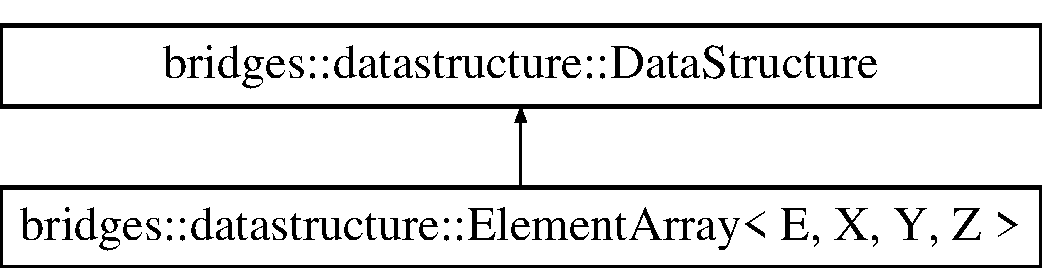
\includegraphics[height=2.000000cm]{classbridges_1_1datastructure_1_1_element_array}
\end{center}
\end{figure}


\doxysubsection{Detailed Description}
\subsubsection*{template$<$typename E, size\+\_\+t X, size\+\_\+t Y = 1, size\+\_\+t Z = 1$>$\newline
class bridges\+::datastructure\+::\+Element\+Array$<$ E, X, Y, Z $>$}

Currently unused class, ignore. \doxysubsection*{Public Member Functions}
\begin{DoxyCompactItemize}
\item 
\mbox{\hyperlink{classbridges_1_1datastructure_1_1_element_array_ae86caf35a947e3b34a2d2bd421e414eb}{Element\+Array}} ()
\item 
\mbox{\hyperlink{classbridges_1_1datastructure_1_1_element}{Element}}$<$ E $>$ $\ast$ \mbox{\hyperlink{classbridges_1_1datastructure_1_1_element_array_a383d08e16eeeb06217d030ed2b18fb37}{get\+Value}} (size\+\_\+t x, size\+\_\+t y=0, size\+\_\+t z=0)
\item 
const \mbox{\hyperlink{classbridges_1_1datastructure_1_1_element}{Element}}$<$ E $>$ $\ast$ \mbox{\hyperlink{classbridges_1_1datastructure_1_1_element_array_a1b05a90e5611a83a4a0c2b535d134303}{get\+Value}} (size\+\_\+t x, size\+\_\+t y=0, size\+\_\+t z=0) const
\item 
void \mbox{\hyperlink{classbridges_1_1datastructure_1_1_element_array_aecd1e6ae5a15c74837f2bfe9d7fbeb60}{set\+Value}} (\mbox{\hyperlink{classbridges_1_1datastructure_1_1_element}{Element}}$<$ E $>$ $\ast$el, size\+\_\+t x, size\+\_\+t y=0, size\+\_\+t z=0)
\item 
virtual const string \mbox{\hyperlink{classbridges_1_1datastructure_1_1_element_array_a22d8c37e88616105cdb7c755f99fdb20}{get\+DStype}} () const override
\end{DoxyCompactItemize}


\doxysubsection{Constructor \& Destructor Documentation}
\mbox{\Hypertarget{classbridges_1_1datastructure_1_1_element_array_ae86caf35a947e3b34a2d2bd421e414eb}\label{classbridges_1_1datastructure_1_1_element_array_ae86caf35a947e3b34a2d2bd421e414eb}} 
\index{bridges::datastructure::ElementArray$<$ E, X, Y, Z $>$@{bridges::datastructure::ElementArray$<$ E, X, Y, Z $>$}!ElementArray@{ElementArray}}
\index{ElementArray@{ElementArray}!bridges::datastructure::ElementArray$<$ E, X, Y, Z $>$@{bridges::datastructure::ElementArray$<$ E, X, Y, Z $>$}}
\doxysubsubsection{\texorpdfstring{ElementArray()}{ElementArray()}}
{\footnotesize\ttfamily template$<$typename E , size\+\_\+t X, size\+\_\+t Y = 1, size\+\_\+t Z = 1$>$ \\
\mbox{\hyperlink{classbridges_1_1datastructure_1_1_element_array}{bridges\+::datastructure\+::\+Element\+Array}}$<$ E, X, Y, Z $>$\+::\mbox{\hyperlink{classbridges_1_1datastructure_1_1_element_array}{Element\+Array}} (\begin{DoxyParamCaption}{ }\end{DoxyParamCaption})\hspace{0.3cm}{\ttfamily [inline]}}



\doxysubsection{Member Function Documentation}
\mbox{\Hypertarget{classbridges_1_1datastructure_1_1_element_array_a22d8c37e88616105cdb7c755f99fdb20}\label{classbridges_1_1datastructure_1_1_element_array_a22d8c37e88616105cdb7c755f99fdb20}} 
\index{bridges::datastructure::ElementArray$<$ E, X, Y, Z $>$@{bridges::datastructure::ElementArray$<$ E, X, Y, Z $>$}!getDStype@{getDStype}}
\index{getDStype@{getDStype}!bridges::datastructure::ElementArray$<$ E, X, Y, Z $>$@{bridges::datastructure::ElementArray$<$ E, X, Y, Z $>$}}
\doxysubsubsection{\texorpdfstring{getDStype()}{getDStype()}}
{\footnotesize\ttfamily template$<$typename E , size\+\_\+t X, size\+\_\+t Y = 1, size\+\_\+t Z = 1$>$ \\
virtual const string \mbox{\hyperlink{classbridges_1_1datastructure_1_1_element_array}{bridges\+::datastructure\+::\+Element\+Array}}$<$ E, X, Y, Z $>$\+::get\+DStype (\begin{DoxyParamCaption}{ }\end{DoxyParamCaption}) const\hspace{0.3cm}{\ttfamily [inline]}, {\ttfamily [override]}, {\ttfamily [virtual]}}

\begin{DoxyReturn}{Returns}
The string representation of this data structure type 
\end{DoxyReturn}


Implements \mbox{\hyperlink{classbridges_1_1datastructure_1_1_data_structure_a4ff66cb34409f11fe9fc647f6d8a22ce}{bridges\+::datastructure\+::\+Data\+Structure}}.

\mbox{\Hypertarget{classbridges_1_1datastructure_1_1_element_array_a383d08e16eeeb06217d030ed2b18fb37}\label{classbridges_1_1datastructure_1_1_element_array_a383d08e16eeeb06217d030ed2b18fb37}} 
\index{bridges::datastructure::ElementArray$<$ E, X, Y, Z $>$@{bridges::datastructure::ElementArray$<$ E, X, Y, Z $>$}!getValue@{getValue}}
\index{getValue@{getValue}!bridges::datastructure::ElementArray$<$ E, X, Y, Z $>$@{bridges::datastructure::ElementArray$<$ E, X, Y, Z $>$}}
\doxysubsubsection{\texorpdfstring{getValue()}{getValue()}\hspace{0.1cm}{\footnotesize\ttfamily [1/2]}}
{\footnotesize\ttfamily template$<$typename E , size\+\_\+t X, size\+\_\+t Y = 1, size\+\_\+t Z = 1$>$ \\
\mbox{\hyperlink{classbridges_1_1datastructure_1_1_element}{Element}}$<$E$>$$\ast$ \mbox{\hyperlink{classbridges_1_1datastructure_1_1_element_array}{bridges\+::datastructure\+::\+Element\+Array}}$<$ E, X, Y, Z $>$\+::get\+Value (\begin{DoxyParamCaption}\item[{size\+\_\+t}]{x,  }\item[{size\+\_\+t}]{y = {\ttfamily 0},  }\item[{size\+\_\+t}]{z = {\ttfamily 0} }\end{DoxyParamCaption})\hspace{0.3cm}{\ttfamily [inline]}}

\mbox{\Hypertarget{classbridges_1_1datastructure_1_1_element_array_a1b05a90e5611a83a4a0c2b535d134303}\label{classbridges_1_1datastructure_1_1_element_array_a1b05a90e5611a83a4a0c2b535d134303}} 
\index{bridges::datastructure::ElementArray$<$ E, X, Y, Z $>$@{bridges::datastructure::ElementArray$<$ E, X, Y, Z $>$}!getValue@{getValue}}
\index{getValue@{getValue}!bridges::datastructure::ElementArray$<$ E, X, Y, Z $>$@{bridges::datastructure::ElementArray$<$ E, X, Y, Z $>$}}
\doxysubsubsection{\texorpdfstring{getValue()}{getValue()}\hspace{0.1cm}{\footnotesize\ttfamily [2/2]}}
{\footnotesize\ttfamily template$<$typename E , size\+\_\+t X, size\+\_\+t Y = 1, size\+\_\+t Z = 1$>$ \\
const \mbox{\hyperlink{classbridges_1_1datastructure_1_1_element}{Element}}$<$E$>$$\ast$ \mbox{\hyperlink{classbridges_1_1datastructure_1_1_element_array}{bridges\+::datastructure\+::\+Element\+Array}}$<$ E, X, Y, Z $>$\+::get\+Value (\begin{DoxyParamCaption}\item[{size\+\_\+t}]{x,  }\item[{size\+\_\+t}]{y = {\ttfamily 0},  }\item[{size\+\_\+t}]{z = {\ttfamily 0} }\end{DoxyParamCaption}) const\hspace{0.3cm}{\ttfamily [inline]}}

\mbox{\Hypertarget{classbridges_1_1datastructure_1_1_element_array_aecd1e6ae5a15c74837f2bfe9d7fbeb60}\label{classbridges_1_1datastructure_1_1_element_array_aecd1e6ae5a15c74837f2bfe9d7fbeb60}} 
\index{bridges::datastructure::ElementArray$<$ E, X, Y, Z $>$@{bridges::datastructure::ElementArray$<$ E, X, Y, Z $>$}!setValue@{setValue}}
\index{setValue@{setValue}!bridges::datastructure::ElementArray$<$ E, X, Y, Z $>$@{bridges::datastructure::ElementArray$<$ E, X, Y, Z $>$}}
\doxysubsubsection{\texorpdfstring{setValue()}{setValue()}}
{\footnotesize\ttfamily template$<$typename E , size\+\_\+t X, size\+\_\+t Y = 1, size\+\_\+t Z = 1$>$ \\
void \mbox{\hyperlink{classbridges_1_1datastructure_1_1_element_array}{bridges\+::datastructure\+::\+Element\+Array}}$<$ E, X, Y, Z $>$\+::set\+Value (\begin{DoxyParamCaption}\item[{\mbox{\hyperlink{classbridges_1_1datastructure_1_1_element}{Element}}$<$ E $>$ $\ast$}]{el,  }\item[{size\+\_\+t}]{x,  }\item[{size\+\_\+t}]{y = {\ttfamily 0},  }\item[{size\+\_\+t}]{z = {\ttfamily 0} }\end{DoxyParamCaption})\hspace{0.3cm}{\ttfamily [inline]}}



The documentation for this class was generated from the following file\+:\begin{DoxyCompactItemize}
\item 
/home/erik/work/bridges/bridges-\/cxx/src/\mbox{\hyperlink{_element_array_8h}{Element\+Array.\+h}}\end{DoxyCompactItemize}

\hypertarget{classbridges_1_1datastructure_1_1_element_visualizer}{}\section{bridges\+::datastructure\+::Element\+Visualizer Class Reference}
\label{classbridges_1_1datastructure_1_1_element_visualizer}\index{bridges::datastructure::ElementVisualizer@{bridges::datastructure::ElementVisualizer}}


{\ttfamily \#include $<$Element\+Visualizer.\+h$>$}



\subsection{Detailed Description}
This class maintains the visual properties of the a \mbox{\hyperlink{classbridges_1_1_bridges}{Bridges}} element. 

This class is used to store the visualization elements for \mbox{\hyperlink{classbridges_1_1_bridges}{Bridges}} Visualiztions, including the color, shape, and size of the node. Defaults of green, circle, and 10.\+0 respectively.

Size values must range from \mbox{[}1.\+0,50.\+0\mbox{]}.

B\+R\+I\+D\+G\+ES supports the shapes listed in Shape (\char`\"{}circle\char`\"{}, \char`\"{}square\char`\"{}, \char`\"{}diamond\char`\"{}, \char`\"{}cross\char`\"{}, \char`\"{}wye\char`\"{}, \char`\"{}triangle\char`\"{}, \char`\"{}star\char`\"{}).

Objects of this class are stored as properties of all \mbox{\hyperlink{classbridges_1_1datastructure_1_1_element}{Element}} subclasses.

\begin{DoxyAuthor}{Author}
Kalpathi Subramanian 
\end{DoxyAuthor}
\begin{DoxyDate}{Date}
6/11/15, 7/12/19 
\end{DoxyDate}
\subsection*{Public Member Functions}
\begin{DoxyCompactItemize}
\item 
\mbox{\hyperlink{classbridges_1_1datastructure_1_1_element_visualizer_a8104e42b94927a9b45a237064d75ca33}{Element\+Visualizer}} (const \mbox{\hyperlink{classbridges_1_1datastructure_1_1_color}{Color}} \&hue=\mbox{\hyperlink{classbridges_1_1datastructure_1_1_element_visualizer_a777a0295e8216e403108a6c90ce6790b}{D\+E\+F\+A\+U\+L\+T\+\_\+\+C\+O\+L\+OR}}(), const double \&sz=\mbox{\hyperlink{classbridges_1_1datastructure_1_1_element_visualizer_afa0fa3f844171f311c3d9c9025a826c5}{D\+E\+F\+A\+U\+L\+T\+\_\+\+S\+I\+ZE}}(), const \mbox{\hyperlink{namespacebridges_1_1datastructure_a3408f5f44d9c6062e5f3adb7e1bbb7f0}{Shape}} \&shp=\mbox{\hyperlink{classbridges_1_1datastructure_1_1_element_visualizer_adfba1c4d4f04ff92545d932bfce5b9d1}{D\+E\+F\+A\+U\+L\+T\+\_\+\+S\+H\+A\+PE}}())
\item 
void \mbox{\hyperlink{classbridges_1_1datastructure_1_1_element_visualizer_a021333b1c20dd55627ac80ae3a2138e6}{set\+Size}} (const double \&sz)
\item 
double \mbox{\hyperlink{classbridges_1_1datastructure_1_1_element_visualizer_a5c83b976308b254521189280bfbfbc43}{get\+Size}} () const
\item 
void \mbox{\hyperlink{classbridges_1_1datastructure_1_1_element_visualizer_aabf1373100f7c45b71d0caf04427644f}{set\+Color}} (const \mbox{\hyperlink{classbridges_1_1datastructure_1_1_color}{Color}} \&col)
\begin{DoxyCompactList}\small\item\em Set the color to \char`\"{}col\char`\"{}. \end{DoxyCompactList}\item 
void \mbox{\hyperlink{classbridges_1_1datastructure_1_1_element_visualizer_a0068ebe250375b13c5b3d4af0df20dea}{set\+Color}} (const string \&col)
\begin{DoxyCompactList}\small\item\em Set the color to a named color. \end{DoxyCompactList}\item 
\mbox{\hyperlink{classbridges_1_1datastructure_1_1_color}{Color}} \mbox{\hyperlink{classbridges_1_1datastructure_1_1_element_visualizer_a611005282caa27575cf3ee7e3b1540c4}{get\+Color}} () const
\item 
void \mbox{\hyperlink{classbridges_1_1datastructure_1_1_element_visualizer_a03f0ba203affb77d4ba8d2f1a6b1eea0}{set\+Opacity}} (double opacity)
\item 
double \mbox{\hyperlink{classbridges_1_1datastructure_1_1_element_visualizer_af403e841efd1dab3669fdda2fd927f99}{get\+Opacity}} ()
\begin{DoxyCompactList}\small\item\em Get opacity of element. \end{DoxyCompactList}\item 
void \mbox{\hyperlink{classbridges_1_1datastructure_1_1_element_visualizer_a316cccfc1e75ccbfdfe6d68da824b8b3}{set\+Shape}} (const \mbox{\hyperlink{namespacebridges_1_1datastructure_a3408f5f44d9c6062e5f3adb7e1bbb7f0}{Shape}} \&shp)
\begin{DoxyCompactList}\small\item\em Set the shape of the element. \end{DoxyCompactList}\item 
\mbox{\hyperlink{namespacebridges_1_1datastructure_a3408f5f44d9c6062e5f3adb7e1bbb7f0}{Shape}} \mbox{\hyperlink{classbridges_1_1datastructure_1_1_element_visualizer_a3b1dd1d61f43844142adce1f0bd03dcf}{get\+Shape}} () const
\begin{DoxyCompactList}\small\item\em Return the shape of the element. \end{DoxyCompactList}\item 
void \mbox{\hyperlink{classbridges_1_1datastructure_1_1_element_visualizer_ae980cb185ddb11ecd1cebeb4834734bf}{set\+Location}} (const double \&locX, const double \&locY)
\item 
double \mbox{\hyperlink{classbridges_1_1datastructure_1_1_element_visualizer_a8ee6ac3a3b03194d51cfbc08a1360b5d}{get\+LocationX}} () const
\item 
double \mbox{\hyperlink{classbridges_1_1datastructure_1_1_element_visualizer_a6012c9545e56e6210b6a6485873a5c92}{get\+LocationY}} () const
\end{DoxyCompactItemize}
\subsection*{Static Public Member Functions}
\begin{DoxyCompactItemize}
\item 
static const \mbox{\hyperlink{classbridges_1_1datastructure_1_1_color}{Color}} \mbox{\hyperlink{classbridges_1_1datastructure_1_1_element_visualizer_a777a0295e8216e403108a6c90ce6790b}{D\+E\+F\+A\+U\+L\+T\+\_\+\+C\+O\+L\+OR}} ()
\item 
static constexpr \mbox{\hyperlink{namespacebridges_1_1datastructure_a3408f5f44d9c6062e5f3adb7e1bbb7f0}{Shape}} \mbox{\hyperlink{classbridges_1_1datastructure_1_1_element_visualizer_adfba1c4d4f04ff92545d932bfce5b9d1}{D\+E\+F\+A\+U\+L\+T\+\_\+\+S\+H\+A\+PE}} ()
\item 
static constexpr double \mbox{\hyperlink{classbridges_1_1datastructure_1_1_element_visualizer_afa0fa3f844171f311c3d9c9025a826c5}{D\+E\+F\+A\+U\+L\+T\+\_\+\+S\+I\+ZE}} ()
\end{DoxyCompactItemize}


\subsection{Constructor \& Destructor Documentation}
\mbox{\Hypertarget{classbridges_1_1datastructure_1_1_element_visualizer_a8104e42b94927a9b45a237064d75ca33}\label{classbridges_1_1datastructure_1_1_element_visualizer_a8104e42b94927a9b45a237064d75ca33}} 
\index{bridges::datastructure::ElementVisualizer@{bridges::datastructure::ElementVisualizer}!ElementVisualizer@{ElementVisualizer}}
\index{ElementVisualizer@{ElementVisualizer}!bridges::datastructure::ElementVisualizer@{bridges::datastructure::ElementVisualizer}}
\subsubsection{\texorpdfstring{ElementVisualizer()}{ElementVisualizer()}}
{\footnotesize\ttfamily bridges\+::datastructure\+::\+Element\+Visualizer\+::\+Element\+Visualizer (\begin{DoxyParamCaption}\item[{const \mbox{\hyperlink{classbridges_1_1datastructure_1_1_color}{Color}} \&}]{hue = {\ttfamily \mbox{\hyperlink{classbridges_1_1datastructure_1_1_element_visualizer_a777a0295e8216e403108a6c90ce6790b}{D\+E\+F\+A\+U\+L\+T\+\_\+\+C\+O\+L\+OR}}()},  }\item[{const double \&}]{sz = {\ttfamily \mbox{\hyperlink{classbridges_1_1datastructure_1_1_element_visualizer_afa0fa3f844171f311c3d9c9025a826c5}{D\+E\+F\+A\+U\+L\+T\+\_\+\+S\+I\+ZE}}()},  }\item[{const \mbox{\hyperlink{namespacebridges_1_1datastructure_a3408f5f44d9c6062e5f3adb7e1bbb7f0}{Shape}} \&}]{shp = {\ttfamily \mbox{\hyperlink{classbridges_1_1datastructure_1_1_element_visualizer_adfba1c4d4f04ff92545d932bfce5b9d1}{D\+E\+F\+A\+U\+L\+T\+\_\+\+S\+H\+A\+PE}}()} }\end{DoxyParamCaption})\hspace{0.3cm}{\ttfamily [inline]}}

Constructs an element with the provided \mbox{\hyperlink{classbridges_1_1datastructure_1_1_color}{Color}}, Size, and Shape. The defaults will be used if not provided.


\begin{DoxyParams}{Parameters}
{\em hue} & The \mbox{\hyperlink{classbridges_1_1datastructure_1_1_color}{Color}} for display \\
\hline
{\em sz} & The Size for display \\
\hline
{\em shp} & The Shape for display \\
\hline
\end{DoxyParams}


\subsection{Member Function Documentation}
\mbox{\Hypertarget{classbridges_1_1datastructure_1_1_element_visualizer_a777a0295e8216e403108a6c90ce6790b}\label{classbridges_1_1datastructure_1_1_element_visualizer_a777a0295e8216e403108a6c90ce6790b}} 
\index{bridges::datastructure::ElementVisualizer@{bridges::datastructure::ElementVisualizer}!DEFAULT\_COLOR@{DEFAULT\_COLOR}}
\index{DEFAULT\_COLOR@{DEFAULT\_COLOR}!bridges::datastructure::ElementVisualizer@{bridges::datastructure::ElementVisualizer}}
\subsubsection{\texorpdfstring{DEFAULT\_COLOR()}{DEFAULT\_COLOR()}}
{\footnotesize\ttfamily static const \mbox{\hyperlink{classbridges_1_1datastructure_1_1_color}{Color}} bridges\+::datastructure\+::\+Element\+Visualizer\+::\+D\+E\+F\+A\+U\+L\+T\+\_\+\+C\+O\+L\+OR (\begin{DoxyParamCaption}{ }\end{DoxyParamCaption})\hspace{0.3cm}{\ttfamily [inline]}, {\ttfamily [static]}}

\mbox{\Hypertarget{classbridges_1_1datastructure_1_1_element_visualizer_adfba1c4d4f04ff92545d932bfce5b9d1}\label{classbridges_1_1datastructure_1_1_element_visualizer_adfba1c4d4f04ff92545d932bfce5b9d1}} 
\index{bridges::datastructure::ElementVisualizer@{bridges::datastructure::ElementVisualizer}!DEFAULT\_SHAPE@{DEFAULT\_SHAPE}}
\index{DEFAULT\_SHAPE@{DEFAULT\_SHAPE}!bridges::datastructure::ElementVisualizer@{bridges::datastructure::ElementVisualizer}}
\subsubsection{\texorpdfstring{DEFAULT\_SHAPE()}{DEFAULT\_SHAPE()}}
{\footnotesize\ttfamily static constexpr \mbox{\hyperlink{namespacebridges_1_1datastructure_a3408f5f44d9c6062e5f3adb7e1bbb7f0}{Shape}} bridges\+::datastructure\+::\+Element\+Visualizer\+::\+D\+E\+F\+A\+U\+L\+T\+\_\+\+S\+H\+A\+PE (\begin{DoxyParamCaption}{ }\end{DoxyParamCaption})\hspace{0.3cm}{\ttfamily [inline]}, {\ttfamily [static]}}

\mbox{\Hypertarget{classbridges_1_1datastructure_1_1_element_visualizer_afa0fa3f844171f311c3d9c9025a826c5}\label{classbridges_1_1datastructure_1_1_element_visualizer_afa0fa3f844171f311c3d9c9025a826c5}} 
\index{bridges::datastructure::ElementVisualizer@{bridges::datastructure::ElementVisualizer}!DEFAULT\_SIZE@{DEFAULT\_SIZE}}
\index{DEFAULT\_SIZE@{DEFAULT\_SIZE}!bridges::datastructure::ElementVisualizer@{bridges::datastructure::ElementVisualizer}}
\subsubsection{\texorpdfstring{DEFAULT\_SIZE()}{DEFAULT\_SIZE()}}
{\footnotesize\ttfamily static constexpr double bridges\+::datastructure\+::\+Element\+Visualizer\+::\+D\+E\+F\+A\+U\+L\+T\+\_\+\+S\+I\+ZE (\begin{DoxyParamCaption}{ }\end{DoxyParamCaption})\hspace{0.3cm}{\ttfamily [inline]}, {\ttfamily [static]}}

\mbox{\Hypertarget{classbridges_1_1datastructure_1_1_element_visualizer_a611005282caa27575cf3ee7e3b1540c4}\label{classbridges_1_1datastructure_1_1_element_visualizer_a611005282caa27575cf3ee7e3b1540c4}} 
\index{bridges::datastructure::ElementVisualizer@{bridges::datastructure::ElementVisualizer}!getColor@{getColor}}
\index{getColor@{getColor}!bridges::datastructure::ElementVisualizer@{bridges::datastructure::ElementVisualizer}}
\subsubsection{\texorpdfstring{getColor()}{getColor()}}
{\footnotesize\ttfamily \mbox{\hyperlink{classbridges_1_1datastructure_1_1_color}{Color}} bridges\+::datastructure\+::\+Element\+Visualizer\+::get\+Color (\begin{DoxyParamCaption}{ }\end{DoxyParamCaption}) const\hspace{0.3cm}{\ttfamily [inline]}}

Return the element color \begin{DoxyReturn}{Returns}
The color of the element 
\end{DoxyReturn}
\mbox{\Hypertarget{classbridges_1_1datastructure_1_1_element_visualizer_a8ee6ac3a3b03194d51cfbc08a1360b5d}\label{classbridges_1_1datastructure_1_1_element_visualizer_a8ee6ac3a3b03194d51cfbc08a1360b5d}} 
\index{bridges::datastructure::ElementVisualizer@{bridges::datastructure::ElementVisualizer}!getLocationX@{getLocationX}}
\index{getLocationX@{getLocationX}!bridges::datastructure::ElementVisualizer@{bridges::datastructure::ElementVisualizer}}
\subsubsection{\texorpdfstring{getLocationX()}{getLocationX()}}
{\footnotesize\ttfamily double bridges\+::datastructure\+::\+Element\+Visualizer\+::get\+LocationX (\begin{DoxyParamCaption}{ }\end{DoxyParamCaption}) const\hspace{0.3cm}{\ttfamily [inline]}}

\begin{DoxyReturn}{Returns}
the X coordinate of the element\textquotesingle{}s location attribute 
\end{DoxyReturn}
\mbox{\Hypertarget{classbridges_1_1datastructure_1_1_element_visualizer_a6012c9545e56e6210b6a6485873a5c92}\label{classbridges_1_1datastructure_1_1_element_visualizer_a6012c9545e56e6210b6a6485873a5c92}} 
\index{bridges::datastructure::ElementVisualizer@{bridges::datastructure::ElementVisualizer}!getLocationY@{getLocationY}}
\index{getLocationY@{getLocationY}!bridges::datastructure::ElementVisualizer@{bridges::datastructure::ElementVisualizer}}
\subsubsection{\texorpdfstring{getLocationY()}{getLocationY()}}
{\footnotesize\ttfamily double bridges\+::datastructure\+::\+Element\+Visualizer\+::get\+LocationY (\begin{DoxyParamCaption}{ }\end{DoxyParamCaption}) const\hspace{0.3cm}{\ttfamily [inline]}}

\begin{DoxyReturn}{Returns}
the Y coordinate of the element\textquotesingle{}s location attribute 
\end{DoxyReturn}
\mbox{\Hypertarget{classbridges_1_1datastructure_1_1_element_visualizer_af403e841efd1dab3669fdda2fd927f99}\label{classbridges_1_1datastructure_1_1_element_visualizer_af403e841efd1dab3669fdda2fd927f99}} 
\index{bridges::datastructure::ElementVisualizer@{bridges::datastructure::ElementVisualizer}!getOpacity@{getOpacity}}
\index{getOpacity@{getOpacity}!bridges::datastructure::ElementVisualizer@{bridges::datastructure::ElementVisualizer}}
\subsubsection{\texorpdfstring{getOpacity()}{getOpacity()}}
{\footnotesize\ttfamily double bridges\+::datastructure\+::\+Element\+Visualizer\+::get\+Opacity (\begin{DoxyParamCaption}{ }\end{DoxyParamCaption})\hspace{0.3cm}{\ttfamily [inline]}}



Get opacity of element. 

\begin{DoxyReturn}{Returns}
opacity 
\end{DoxyReturn}
\mbox{\Hypertarget{classbridges_1_1datastructure_1_1_element_visualizer_a3b1dd1d61f43844142adce1f0bd03dcf}\label{classbridges_1_1datastructure_1_1_element_visualizer_a3b1dd1d61f43844142adce1f0bd03dcf}} 
\index{bridges::datastructure::ElementVisualizer@{bridges::datastructure::ElementVisualizer}!getShape@{getShape}}
\index{getShape@{getShape}!bridges::datastructure::ElementVisualizer@{bridges::datastructure::ElementVisualizer}}
\subsubsection{\texorpdfstring{getShape()}{getShape()}}
{\footnotesize\ttfamily \mbox{\hyperlink{namespacebridges_1_1datastructure_a3408f5f44d9c6062e5f3adb7e1bbb7f0}{Shape}} bridges\+::datastructure\+::\+Element\+Visualizer\+::get\+Shape (\begin{DoxyParamCaption}{ }\end{DoxyParamCaption}) const\hspace{0.3cm}{\ttfamily [inline]}}



Return the shape of the element. 

\begin{DoxyReturn}{Returns}
The shape of the element 
\end{DoxyReturn}
\mbox{\Hypertarget{classbridges_1_1datastructure_1_1_element_visualizer_a5c83b976308b254521189280bfbfbc43}\label{classbridges_1_1datastructure_1_1_element_visualizer_a5c83b976308b254521189280bfbfbc43}} 
\index{bridges::datastructure::ElementVisualizer@{bridges::datastructure::ElementVisualizer}!getSize@{getSize}}
\index{getSize@{getSize}!bridges::datastructure::ElementVisualizer@{bridges::datastructure::ElementVisualizer}}
\subsubsection{\texorpdfstring{getSize()}{getSize()}}
{\footnotesize\ttfamily double bridges\+::datastructure\+::\+Element\+Visualizer\+::get\+Size (\begin{DoxyParamCaption}{ }\end{DoxyParamCaption}) const\hspace{0.3cm}{\ttfamily [inline]}}

\begin{DoxyReturn}{Returns}
The size in pixel weight of the element 
\end{DoxyReturn}
\mbox{\Hypertarget{classbridges_1_1datastructure_1_1_element_visualizer_aabf1373100f7c45b71d0caf04427644f}\label{classbridges_1_1datastructure_1_1_element_visualizer_aabf1373100f7c45b71d0caf04427644f}} 
\index{bridges::datastructure::ElementVisualizer@{bridges::datastructure::ElementVisualizer}!setColor@{setColor}}
\index{setColor@{setColor}!bridges::datastructure::ElementVisualizer@{bridges::datastructure::ElementVisualizer}}
\subsubsection{\texorpdfstring{setColor()}{setColor()}\hspace{0.1cm}{\footnotesize\ttfamily [1/2]}}
{\footnotesize\ttfamily void bridges\+::datastructure\+::\+Element\+Visualizer\+::set\+Color (\begin{DoxyParamCaption}\item[{const \mbox{\hyperlink{classbridges_1_1datastructure_1_1_color}{Color}} \&}]{col }\end{DoxyParamCaption})\hspace{0.3cm}{\ttfamily [inline]}}



Set the color to \char`\"{}col\char`\"{}. 


\begin{DoxyParams}{Parameters}
{\em col} & The color of the element \\
\hline
\end{DoxyParams}
\mbox{\Hypertarget{classbridges_1_1datastructure_1_1_element_visualizer_a0068ebe250375b13c5b3d4af0df20dea}\label{classbridges_1_1datastructure_1_1_element_visualizer_a0068ebe250375b13c5b3d4af0df20dea}} 
\index{bridges::datastructure::ElementVisualizer@{bridges::datastructure::ElementVisualizer}!setColor@{setColor}}
\index{setColor@{setColor}!bridges::datastructure::ElementVisualizer@{bridges::datastructure::ElementVisualizer}}
\subsubsection{\texorpdfstring{setColor()}{setColor()}\hspace{0.1cm}{\footnotesize\ttfamily [2/2]}}
{\footnotesize\ttfamily void bridges\+::datastructure\+::\+Element\+Visualizer\+::set\+Color (\begin{DoxyParamCaption}\item[{const string \&}]{col }\end{DoxyParamCaption})\hspace{0.3cm}{\ttfamily [inline]}}



Set the color to a named color. 


\begin{DoxyParams}{Parameters}
{\em col} & The color name. Check the \mbox{\hyperlink{classbridges_1_1datastructure_1_1_color}{Color}} class for supported values. \\
\hline
\end{DoxyParams}
\mbox{\Hypertarget{classbridges_1_1datastructure_1_1_element_visualizer_ae980cb185ddb11ecd1cebeb4834734bf}\label{classbridges_1_1datastructure_1_1_element_visualizer_ae980cb185ddb11ecd1cebeb4834734bf}} 
\index{bridges::datastructure::ElementVisualizer@{bridges::datastructure::ElementVisualizer}!setLocation@{setLocation}}
\index{setLocation@{setLocation}!bridges::datastructure::ElementVisualizer@{bridges::datastructure::ElementVisualizer}}
\subsubsection{\texorpdfstring{setLocation()}{setLocation()}}
{\footnotesize\ttfamily void bridges\+::datastructure\+::\+Element\+Visualizer\+::set\+Location (\begin{DoxyParamCaption}\item[{const double \&}]{locX,  }\item[{const double \&}]{locY }\end{DoxyParamCaption})\hspace{0.3cm}{\ttfamily [inline]}}

Set the location attributes of an element. Set location to I\+N\+F\+I\+N\+I\+TY for bridges to chose the location.


\begin{DoxyParams}{Parameters}
{\em locX} & X coordinate of the element location \\
\hline
{\em locY} & Y coordinate of the element location \\
\hline
\end{DoxyParams}
\mbox{\Hypertarget{classbridges_1_1datastructure_1_1_element_visualizer_a03f0ba203affb77d4ba8d2f1a6b1eea0}\label{classbridges_1_1datastructure_1_1_element_visualizer_a03f0ba203affb77d4ba8d2f1a6b1eea0}} 
\index{bridges::datastructure::ElementVisualizer@{bridges::datastructure::ElementVisualizer}!setOpacity@{setOpacity}}
\index{setOpacity@{setOpacity}!bridges::datastructure::ElementVisualizer@{bridges::datastructure::ElementVisualizer}}
\subsubsection{\texorpdfstring{setOpacity()}{setOpacity()}}
{\footnotesize\ttfamily void bridges\+::datastructure\+::\+Element\+Visualizer\+::set\+Opacity (\begin{DoxyParamCaption}\item[{double}]{opacity }\end{DoxyParamCaption})\hspace{0.3cm}{\ttfamily [inline]}}

Set opacity of element -\/ use the 4th color component


\begin{DoxyParams}{Parameters}
{\em opacity} & \\
\hline
\end{DoxyParams}
\mbox{\Hypertarget{classbridges_1_1datastructure_1_1_element_visualizer_a316cccfc1e75ccbfdfe6d68da824b8b3}\label{classbridges_1_1datastructure_1_1_element_visualizer_a316cccfc1e75ccbfdfe6d68da824b8b3}} 
\index{bridges::datastructure::ElementVisualizer@{bridges::datastructure::ElementVisualizer}!setShape@{setShape}}
\index{setShape@{setShape}!bridges::datastructure::ElementVisualizer@{bridges::datastructure::ElementVisualizer}}
\subsubsection{\texorpdfstring{setShape()}{setShape()}}
{\footnotesize\ttfamily void bridges\+::datastructure\+::\+Element\+Visualizer\+::set\+Shape (\begin{DoxyParamCaption}\item[{const \mbox{\hyperlink{namespacebridges_1_1datastructure_a3408f5f44d9c6062e5f3adb7e1bbb7f0}{Shape}} \&}]{shp }\end{DoxyParamCaption})\hspace{0.3cm}{\ttfamily [inline]}}



Set the shape of the element. 


\begin{DoxyParams}{Parameters}
{\em shp} & is one of Shape.\+C\+I\+R\+C\+LE, Shape.\+S\+Q\+U\+A\+RE, Shape.\+D\+I\+A\+M\+O\+ND, Shape.\+C\+R\+O\+SS, Shape.\+T\+R\+I\+A\+N\+G\+LE, Shape.\+W\+YE, Shape.\+S\+T\+AR. \\
\hline
\end{DoxyParams}
\mbox{\Hypertarget{classbridges_1_1datastructure_1_1_element_visualizer_a021333b1c20dd55627ac80ae3a2138e6}\label{classbridges_1_1datastructure_1_1_element_visualizer_a021333b1c20dd55627ac80ae3a2138e6}} 
\index{bridges::datastructure::ElementVisualizer@{bridges::datastructure::ElementVisualizer}!setSize@{setSize}}
\index{setSize@{setSize}!bridges::datastructure::ElementVisualizer@{bridges::datastructure::ElementVisualizer}}
\subsubsection{\texorpdfstring{setSize()}{setSize()}}
{\footnotesize\ttfamily void bridges\+::datastructure\+::\+Element\+Visualizer\+::set\+Size (\begin{DoxyParamCaption}\item[{const double \&}]{sz }\end{DoxyParamCaption})\hspace{0.3cm}{\ttfamily [inline]}}

Sets size to \char`\"{}sz\char`\"{} Valid Range\+:\mbox{[}1,50\mbox{]}


\begin{DoxyParams}{Parameters}
{\em sz} & The size in pixel weight of the element \\
\hline
\end{DoxyParams}

\begin{DoxyExceptions}{Exceptions}
{\em string} & If size is invalid \\
\hline
\end{DoxyExceptions}


The documentation for this class was generated from the following file\+:\begin{DoxyCompactItemize}
\item 
/\+Users/kalpathi/gr/bridges/cxx/src/\mbox{\hyperlink{_element_visualizer_8h}{Element\+Visualizer.\+h}}\end{DoxyCompactItemize}

\hypertarget{classbridges_1_1dataset_1_1_elevation_data}{}\section{bridges\+:\+:dataset\+:\+:Elevation\+Data Class Reference}
\label{classbridges_1_1dataset_1_1_elevation_data}\index{bridges\+::dataset\+::\+Elevation\+Data@{bridges\+::dataset\+::\+Elevation\+Data}}


{\ttfamily \#include $<$Elevation\+Data.\+h$>$}



\subsection{Detailed Description}
Class that hold elevation data. 

Class that holds Elevation data, from ??

\begin{DoxyAuthor}{Author}
Kalpathi Subramanian
\end{DoxyAuthor}
\begin{DoxyDate}{Date}
3/28/20 
\end{DoxyDate}
\subsection*{Public Member Functions}
\begin{DoxyCompactItemize}
\item 
\hyperlink{classbridges_1_1dataset_1_1_elevation_data_a5b18c287b0c0030a5e454b705778a3f6}{Elevation\+Data} ()
\item 
\hyperlink{classbridges_1_1dataset_1_1_elevation_data_a89635a4704d9d4f67421661a74cc954d}{Elevation\+Data} (int r, int c)
\item 
\hyperlink{classbridges_1_1dataset_1_1_elevation_data_af51b3b3db6299140005988c03fcd12c9}{Elevation\+Data} (int cols, int rows, int xll, int yll, int cellsize, int max\+Val)
\item 
\hyperlink{classbridges_1_1dataset_1_1_elevation_data_a253e44f5f60891569c21ca926a356547}{$\sim$\+Elevation\+Data} ()
\item 
int \hyperlink{classbridges_1_1dataset_1_1_elevation_data_a9f5d6c6db9861715719485524b10e5d0}{get\+Cols} ()
\item 
void \hyperlink{classbridges_1_1dataset_1_1_elevation_data_adf57abd5e1e058ca6b0eb093aa5c7a11}{set\+Cols} (int c)
\item 
int \hyperlink{classbridges_1_1dataset_1_1_elevation_data_abdc18537c20774cf561d97987f1fb74a}{get\+Val} (int r, int c)
\item 
void \hyperlink{classbridges_1_1dataset_1_1_elevation_data_aa917c02a316f30d8e92d38bfb26fff9a}{set\+Val} (int r, int c, int val)
\item 
int \hyperlink{classbridges_1_1dataset_1_1_elevation_data_a6e721fe05638f95e22aef75f25cd4ae0}{get\+Rows} ()
\item 
void \hyperlink{classbridges_1_1dataset_1_1_elevation_data_a07c1929c481e06e6f1e01495aa319c57}{set\+Rows} (int r)
\item 
int \hyperlink{classbridges_1_1dataset_1_1_elevation_data_a5a4858f48b6f8e85d2210b736c890e91}{getxll} ()
\item 
void \hyperlink{classbridges_1_1dataset_1_1_elevation_data_a95e5b02c45c547908612e83641eb386c}{setxll} (int x\+\_\+ll)
\item 
int \hyperlink{classbridges_1_1dataset_1_1_elevation_data_ab021a75e1f0d606b00afcf57803f3503}{getyll} ()
\item 
void \hyperlink{classbridges_1_1dataset_1_1_elevation_data_a4ea6e380b7cc1531a0ae9b593dd98843}{setyll} (int y\+\_\+ll)
\item 
int \hyperlink{classbridges_1_1dataset_1_1_elevation_data_a04f2482408b57ba8e3823025af1932b6}{get\+Cell\+Size} ()
\item 
void \hyperlink{classbridges_1_1dataset_1_1_elevation_data_a7014a6d2bbc8092995fbbf40d57a3fdf}{set\+Cell\+Size} (int cell\+\_\+size)
\item 
int \hyperlink{classbridges_1_1dataset_1_1_elevation_data_a59dbda36f7635ff382f6a51972f0ed5d}{get\+Max\+Val} ()
\item 
void \hyperlink{classbridges_1_1dataset_1_1_elevation_data_ae21e8da36d7b7ad93121aff7ef6d69ab}{set\+Max\+Val} (int max\+\_\+val)
\end{DoxyCompactItemize}


\subsection{Constructor \& Destructor Documentation}
\mbox{\Hypertarget{classbridges_1_1dataset_1_1_elevation_data_a5b18c287b0c0030a5e454b705778a3f6}\label{classbridges_1_1dataset_1_1_elevation_data_a5b18c287b0c0030a5e454b705778a3f6}} 
\index{bridges\+::dataset\+::\+Elevation\+Data@{bridges\+::dataset\+::\+Elevation\+Data}!Elevation\+Data@{Elevation\+Data}}
\index{Elevation\+Data@{Elevation\+Data}!bridges\+::dataset\+::\+Elevation\+Data@{bridges\+::dataset\+::\+Elevation\+Data}}
\subsubsection{\texorpdfstring{Elevation\+Data()}{ElevationData()}\hspace{0.1cm}{\footnotesize\ttfamily [1/3]}}
{\footnotesize\ttfamily bridges\+::dataset\+::\+Elevation\+Data\+::\+Elevation\+Data (\begin{DoxyParamCaption}{ }\end{DoxyParamCaption})\hspace{0.3cm}{\ttfamily [inline]}}

default constructor \mbox{\Hypertarget{classbridges_1_1dataset_1_1_elevation_data_a89635a4704d9d4f67421661a74cc954d}\label{classbridges_1_1dataset_1_1_elevation_data_a89635a4704d9d4f67421661a74cc954d}} 
\index{bridges\+::dataset\+::\+Elevation\+Data@{bridges\+::dataset\+::\+Elevation\+Data}!Elevation\+Data@{Elevation\+Data}}
\index{Elevation\+Data@{Elevation\+Data}!bridges\+::dataset\+::\+Elevation\+Data@{bridges\+::dataset\+::\+Elevation\+Data}}
\subsubsection{\texorpdfstring{Elevation\+Data()}{ElevationData()}\hspace{0.1cm}{\footnotesize\ttfamily [2/3]}}
{\footnotesize\ttfamily bridges\+::dataset\+::\+Elevation\+Data\+::\+Elevation\+Data (\begin{DoxyParamCaption}\item[{int}]{r,  }\item[{int}]{c }\end{DoxyParamCaption})\hspace{0.3cm}{\ttfamily [inline]}}

constructor 
\begin{DoxyParams}{Parameters}
{\em r} & number of rows (height) of elevation map \\
\hline
{\em c} & number of columns (width) of elevation map \\
\hline
\end{DoxyParams}
\mbox{\Hypertarget{classbridges_1_1dataset_1_1_elevation_data_af51b3b3db6299140005988c03fcd12c9}\label{classbridges_1_1dataset_1_1_elevation_data_af51b3b3db6299140005988c03fcd12c9}} 
\index{bridges\+::dataset\+::\+Elevation\+Data@{bridges\+::dataset\+::\+Elevation\+Data}!Elevation\+Data@{Elevation\+Data}}
\index{Elevation\+Data@{Elevation\+Data}!bridges\+::dataset\+::\+Elevation\+Data@{bridges\+::dataset\+::\+Elevation\+Data}}
\subsubsection{\texorpdfstring{Elevation\+Data()}{ElevationData()}\hspace{0.1cm}{\footnotesize\ttfamily [3/3]}}
{\footnotesize\ttfamily bridges\+::dataset\+::\+Elevation\+Data\+::\+Elevation\+Data (\begin{DoxyParamCaption}\item[{int}]{cols,  }\item[{int}]{rows,  }\item[{int}]{xll,  }\item[{int}]{yll,  }\item[{int}]{cellsize,  }\item[{int}]{max\+Val }\end{DoxyParamCaption})\hspace{0.3cm}{\ttfamily [inline]}}

constructor 
\begin{DoxyParams}{Parameters}
{\em rows} & number of rows (height) of elevation map \\
\hline
{\em cols} & number of columns (width) of elevation map \\
\hline
{\em xll} & lower left of map -\/ x coordinate \\
\hline
{\em yll} & lower left of map -\/ y coordinate \\
\hline
{\em cellsize} & size of each cell \\
\hline
{\em max\+Val} & max elevation value in map \\
\hline
\end{DoxyParams}
\mbox{\Hypertarget{classbridges_1_1dataset_1_1_elevation_data_a253e44f5f60891569c21ca926a356547}\label{classbridges_1_1dataset_1_1_elevation_data_a253e44f5f60891569c21ca926a356547}} 
\index{bridges\+::dataset\+::\+Elevation\+Data@{bridges\+::dataset\+::\+Elevation\+Data}!````~Elevation\+Data@{$\sim$\+Elevation\+Data}}
\index{````~Elevation\+Data@{$\sim$\+Elevation\+Data}!bridges\+::dataset\+::\+Elevation\+Data@{bridges\+::dataset\+::\+Elevation\+Data}}
\subsubsection{\texorpdfstring{$\sim$\+Elevation\+Data()}{~ElevationData()}}
{\footnotesize\ttfamily bridges\+::dataset\+::\+Elevation\+Data\+::$\sim$\+Elevation\+Data (\begin{DoxyParamCaption}{ }\end{DoxyParamCaption})\hspace{0.3cm}{\ttfamily [inline]}}

destructor 

\subsection{Member Function Documentation}
\mbox{\Hypertarget{classbridges_1_1dataset_1_1_elevation_data_a04f2482408b57ba8e3823025af1932b6}\label{classbridges_1_1dataset_1_1_elevation_data_a04f2482408b57ba8e3823025af1932b6}} 
\index{bridges\+::dataset\+::\+Elevation\+Data@{bridges\+::dataset\+::\+Elevation\+Data}!get\+Cell\+Size@{get\+Cell\+Size}}
\index{get\+Cell\+Size@{get\+Cell\+Size}!bridges\+::dataset\+::\+Elevation\+Data@{bridges\+::dataset\+::\+Elevation\+Data}}
\subsubsection{\texorpdfstring{get\+Cell\+Size()}{getCellSize()}}
{\footnotesize\ttfamily int bridges\+::dataset\+::\+Elevation\+Data\+::get\+Cell\+Size (\begin{DoxyParamCaption}{ }\end{DoxyParamCaption})\hspace{0.3cm}{\ttfamily [inline]}}

get data resolution \begin{DoxyReturn}{Returns}
the cell size 
\end{DoxyReturn}
\mbox{\Hypertarget{classbridges_1_1dataset_1_1_elevation_data_a9f5d6c6db9861715719485524b10e5d0}\label{classbridges_1_1dataset_1_1_elevation_data_a9f5d6c6db9861715719485524b10e5d0}} 
\index{bridges\+::dataset\+::\+Elevation\+Data@{bridges\+::dataset\+::\+Elevation\+Data}!get\+Cols@{get\+Cols}}
\index{get\+Cols@{get\+Cols}!bridges\+::dataset\+::\+Elevation\+Data@{bridges\+::dataset\+::\+Elevation\+Data}}
\subsubsection{\texorpdfstring{get\+Cols()}{getCols()}}
{\footnotesize\ttfamily int bridges\+::dataset\+::\+Elevation\+Data\+::get\+Cols (\begin{DoxyParamCaption}{ }\end{DoxyParamCaption})\hspace{0.3cm}{\ttfamily [inline]}}

get width of elevation map \begin{DoxyReturn}{Returns}
width of map 
\end{DoxyReturn}
\mbox{\Hypertarget{classbridges_1_1dataset_1_1_elevation_data_a59dbda36f7635ff382f6a51972f0ed5d}\label{classbridges_1_1dataset_1_1_elevation_data_a59dbda36f7635ff382f6a51972f0ed5d}} 
\index{bridges\+::dataset\+::\+Elevation\+Data@{bridges\+::dataset\+::\+Elevation\+Data}!get\+Max\+Val@{get\+Max\+Val}}
\index{get\+Max\+Val@{get\+Max\+Val}!bridges\+::dataset\+::\+Elevation\+Data@{bridges\+::dataset\+::\+Elevation\+Data}}
\subsubsection{\texorpdfstring{get\+Max\+Val()}{getMaxVal()}}
{\footnotesize\ttfamily int bridges\+::dataset\+::\+Elevation\+Data\+::get\+Max\+Val (\begin{DoxyParamCaption}{ }\end{DoxyParamCaption})\hspace{0.3cm}{\ttfamily [inline]}}

get max elevation of data \begin{DoxyReturn}{Returns}
the max elevation value in the map 
\end{DoxyReturn}
\mbox{\Hypertarget{classbridges_1_1dataset_1_1_elevation_data_a6e721fe05638f95e22aef75f25cd4ae0}\label{classbridges_1_1dataset_1_1_elevation_data_a6e721fe05638f95e22aef75f25cd4ae0}} 
\index{bridges\+::dataset\+::\+Elevation\+Data@{bridges\+::dataset\+::\+Elevation\+Data}!get\+Rows@{get\+Rows}}
\index{get\+Rows@{get\+Rows}!bridges\+::dataset\+::\+Elevation\+Data@{bridges\+::dataset\+::\+Elevation\+Data}}
\subsubsection{\texorpdfstring{get\+Rows()}{getRows()}}
{\footnotesize\ttfamily int bridges\+::dataset\+::\+Elevation\+Data\+::get\+Rows (\begin{DoxyParamCaption}{ }\end{DoxyParamCaption})\hspace{0.3cm}{\ttfamily [inline]}}

get num rows of data

\begin{DoxyReturn}{Returns}
width of elevation map 
\end{DoxyReturn}
\mbox{\Hypertarget{classbridges_1_1dataset_1_1_elevation_data_abdc18537c20774cf561d97987f1fb74a}\label{classbridges_1_1dataset_1_1_elevation_data_abdc18537c20774cf561d97987f1fb74a}} 
\index{bridges\+::dataset\+::\+Elevation\+Data@{bridges\+::dataset\+::\+Elevation\+Data}!get\+Val@{get\+Val}}
\index{get\+Val@{get\+Val}!bridges\+::dataset\+::\+Elevation\+Data@{bridges\+::dataset\+::\+Elevation\+Data}}
\subsubsection{\texorpdfstring{get\+Val()}{getVal()}}
{\footnotesize\ttfamily int bridges\+::dataset\+::\+Elevation\+Data\+::get\+Val (\begin{DoxyParamCaption}\item[{int}]{r,  }\item[{int}]{c }\end{DoxyParamCaption})\hspace{0.3cm}{\ttfamily [inline]}}

get width of elevation map


\begin{DoxyParams}{Parameters}
{\em r} & row index \\
\hline
{\em c} & column index \\
\hline
\end{DoxyParams}
\mbox{\Hypertarget{classbridges_1_1dataset_1_1_elevation_data_a5a4858f48b6f8e85d2210b736c890e91}\label{classbridges_1_1dataset_1_1_elevation_data_a5a4858f48b6f8e85d2210b736c890e91}} 
\index{bridges\+::dataset\+::\+Elevation\+Data@{bridges\+::dataset\+::\+Elevation\+Data}!getxll@{getxll}}
\index{getxll@{getxll}!bridges\+::dataset\+::\+Elevation\+Data@{bridges\+::dataset\+::\+Elevation\+Data}}
\subsubsection{\texorpdfstring{getxll()}{getxll()}}
{\footnotesize\ttfamily int bridges\+::dataset\+::\+Elevation\+Data\+::getxll (\begin{DoxyParamCaption}{ }\end{DoxyParamCaption})\hspace{0.3cm}{\ttfamily [inline]}}

get lower left corner of data (X) \begin{DoxyReturn}{Returns}
x coord of lower left of map 
\end{DoxyReturn}
\mbox{\Hypertarget{classbridges_1_1dataset_1_1_elevation_data_ab021a75e1f0d606b00afcf57803f3503}\label{classbridges_1_1dataset_1_1_elevation_data_ab021a75e1f0d606b00afcf57803f3503}} 
\index{bridges\+::dataset\+::\+Elevation\+Data@{bridges\+::dataset\+::\+Elevation\+Data}!getyll@{getyll}}
\index{getyll@{getyll}!bridges\+::dataset\+::\+Elevation\+Data@{bridges\+::dataset\+::\+Elevation\+Data}}
\subsubsection{\texorpdfstring{getyll()}{getyll()}}
{\footnotesize\ttfamily int bridges\+::dataset\+::\+Elevation\+Data\+::getyll (\begin{DoxyParamCaption}{ }\end{DoxyParamCaption})\hspace{0.3cm}{\ttfamily [inline]}}

get lower left corner of data (Y) \begin{DoxyReturn}{Returns}
y coord of lower left of map 
\end{DoxyReturn}
\mbox{\Hypertarget{classbridges_1_1dataset_1_1_elevation_data_a7014a6d2bbc8092995fbbf40d57a3fdf}\label{classbridges_1_1dataset_1_1_elevation_data_a7014a6d2bbc8092995fbbf40d57a3fdf}} 
\index{bridges\+::dataset\+::\+Elevation\+Data@{bridges\+::dataset\+::\+Elevation\+Data}!set\+Cell\+Size@{set\+Cell\+Size}}
\index{set\+Cell\+Size@{set\+Cell\+Size}!bridges\+::dataset\+::\+Elevation\+Data@{bridges\+::dataset\+::\+Elevation\+Data}}
\subsubsection{\texorpdfstring{set\+Cell\+Size()}{setCellSize()}}
{\footnotesize\ttfamily void bridges\+::dataset\+::\+Elevation\+Data\+::set\+Cell\+Size (\begin{DoxyParamCaption}\item[{int}]{cell\+\_\+size }\end{DoxyParamCaption})\hspace{0.3cm}{\ttfamily [inline]}}

set data resolution 
\begin{DoxyParams}{Parameters}
{\em cell\+\_\+size} & set the resolution of the map to cell\+\_\+size \\
\hline
\end{DoxyParams}
\mbox{\Hypertarget{classbridges_1_1dataset_1_1_elevation_data_adf57abd5e1e058ca6b0eb093aa5c7a11}\label{classbridges_1_1dataset_1_1_elevation_data_adf57abd5e1e058ca6b0eb093aa5c7a11}} 
\index{bridges\+::dataset\+::\+Elevation\+Data@{bridges\+::dataset\+::\+Elevation\+Data}!set\+Cols@{set\+Cols}}
\index{set\+Cols@{set\+Cols}!bridges\+::dataset\+::\+Elevation\+Data@{bridges\+::dataset\+::\+Elevation\+Data}}
\subsubsection{\texorpdfstring{set\+Cols()}{setCols()}}
{\footnotesize\ttfamily void bridges\+::dataset\+::\+Elevation\+Data\+::set\+Cols (\begin{DoxyParamCaption}\item[{int}]{c }\end{DoxyParamCaption})\hspace{0.3cm}{\ttfamily [inline]}}

set width of elevation map 
\begin{DoxyParams}{Parameters}
{\em c} & width of map \\
\hline
\end{DoxyParams}
\mbox{\Hypertarget{classbridges_1_1dataset_1_1_elevation_data_ae21e8da36d7b7ad93121aff7ef6d69ab}\label{classbridges_1_1dataset_1_1_elevation_data_ae21e8da36d7b7ad93121aff7ef6d69ab}} 
\index{bridges\+::dataset\+::\+Elevation\+Data@{bridges\+::dataset\+::\+Elevation\+Data}!set\+Max\+Val@{set\+Max\+Val}}
\index{set\+Max\+Val@{set\+Max\+Val}!bridges\+::dataset\+::\+Elevation\+Data@{bridges\+::dataset\+::\+Elevation\+Data}}
\subsubsection{\texorpdfstring{set\+Max\+Val()}{setMaxVal()}}
{\footnotesize\ttfamily void bridges\+::dataset\+::\+Elevation\+Data\+::set\+Max\+Val (\begin{DoxyParamCaption}\item[{int}]{max\+\_\+val }\end{DoxyParamCaption})\hspace{0.3cm}{\ttfamily [inline]}}

set max elevation of data 
\begin{DoxyParams}{Parameters}
{\em max\+\_\+val} & the max value of elevation to set \\
\hline
\end{DoxyParams}
\mbox{\Hypertarget{classbridges_1_1dataset_1_1_elevation_data_a07c1929c481e06e6f1e01495aa319c57}\label{classbridges_1_1dataset_1_1_elevation_data_a07c1929c481e06e6f1e01495aa319c57}} 
\index{bridges\+::dataset\+::\+Elevation\+Data@{bridges\+::dataset\+::\+Elevation\+Data}!set\+Rows@{set\+Rows}}
\index{set\+Rows@{set\+Rows}!bridges\+::dataset\+::\+Elevation\+Data@{bridges\+::dataset\+::\+Elevation\+Data}}
\subsubsection{\texorpdfstring{set\+Rows()}{setRows()}}
{\footnotesize\ttfamily void bridges\+::dataset\+::\+Elevation\+Data\+::set\+Rows (\begin{DoxyParamCaption}\item[{int}]{r }\end{DoxyParamCaption})\hspace{0.3cm}{\ttfamily [inline]}}

set num rows of data


\begin{DoxyParams}{Parameters}
{\em r} & width of elevation map to set \\
\hline
\end{DoxyParams}
\mbox{\Hypertarget{classbridges_1_1dataset_1_1_elevation_data_aa917c02a316f30d8e92d38bfb26fff9a}\label{classbridges_1_1dataset_1_1_elevation_data_aa917c02a316f30d8e92d38bfb26fff9a}} 
\index{bridges\+::dataset\+::\+Elevation\+Data@{bridges\+::dataset\+::\+Elevation\+Data}!set\+Val@{set\+Val}}
\index{set\+Val@{set\+Val}!bridges\+::dataset\+::\+Elevation\+Data@{bridges\+::dataset\+::\+Elevation\+Data}}
\subsubsection{\texorpdfstring{set\+Val()}{setVal()}}
{\footnotesize\ttfamily void bridges\+::dataset\+::\+Elevation\+Data\+::set\+Val (\begin{DoxyParamCaption}\item[{int}]{r,  }\item[{int}]{c,  }\item[{int}]{val }\end{DoxyParamCaption})\hspace{0.3cm}{\ttfamily [inline]}}

set elevation value at row r and column c


\begin{DoxyParams}{Parameters}
{\em r} & row index \\
\hline
{\em c} & column index \\
\hline
{\em val} & elevation value \\
\hline
\end{DoxyParams}
\mbox{\Hypertarget{classbridges_1_1dataset_1_1_elevation_data_a95e5b02c45c547908612e83641eb386c}\label{classbridges_1_1dataset_1_1_elevation_data_a95e5b02c45c547908612e83641eb386c}} 
\index{bridges\+::dataset\+::\+Elevation\+Data@{bridges\+::dataset\+::\+Elevation\+Data}!setxll@{setxll}}
\index{setxll@{setxll}!bridges\+::dataset\+::\+Elevation\+Data@{bridges\+::dataset\+::\+Elevation\+Data}}
\subsubsection{\texorpdfstring{setxll()}{setxll()}}
{\footnotesize\ttfamily void bridges\+::dataset\+::\+Elevation\+Data\+::setxll (\begin{DoxyParamCaption}\item[{int}]{x\+\_\+ll }\end{DoxyParamCaption})\hspace{0.3cm}{\ttfamily [inline]}}

set lower left corner of data (X)


\begin{DoxyParams}{Parameters}
{\em x\+\_\+ll} & lower left coord of X to set \\
\hline
\end{DoxyParams}
\mbox{\Hypertarget{classbridges_1_1dataset_1_1_elevation_data_a4ea6e380b7cc1531a0ae9b593dd98843}\label{classbridges_1_1dataset_1_1_elevation_data_a4ea6e380b7cc1531a0ae9b593dd98843}} 
\index{bridges\+::dataset\+::\+Elevation\+Data@{bridges\+::dataset\+::\+Elevation\+Data}!setyll@{setyll}}
\index{setyll@{setyll}!bridges\+::dataset\+::\+Elevation\+Data@{bridges\+::dataset\+::\+Elevation\+Data}}
\subsubsection{\texorpdfstring{setyll()}{setyll()}}
{\footnotesize\ttfamily void bridges\+::dataset\+::\+Elevation\+Data\+::setyll (\begin{DoxyParamCaption}\item[{int}]{y\+\_\+ll }\end{DoxyParamCaption})\hspace{0.3cm}{\ttfamily [inline]}}

set lower left corner of data (Y) 
\begin{DoxyParams}{Parameters}
{\em y\+\_\+ll} & lower left coord of Y to set \\
\hline
\end{DoxyParams}


The documentation for this class was generated from the following file\+:\begin{DoxyCompactItemize}
\item 
/home/erik/work/bridges/bridges-\/cxx/src/data\+\_\+src/\hyperlink{_elevation_data_8h}{Elevation\+Data.\+h}\end{DoxyCompactItemize}

\hypertarget{classsio_1_1event}{}\section{sio\+:\+:event Class Reference}
\label{classsio_1_1event}\index{sio\+::event@{sio\+::event}}


{\ttfamily \#include $<$sio\+\_\+socket.\+h$>$}

\subsection*{Public Member Functions}
\begin{DoxyCompactItemize}
\item 
const std\+::string \& \hyperlink{classsio_1_1event_a248d2f8a20d6915059ec8cee5cf7449d}{get\+\_\+nsp} () const
\item 
const std\+::string \& \hyperlink{classsio_1_1event_ac5049d464f6b37a92739bbbaee700f7f}{get\+\_\+name} () const
\item 
const \hyperlink{classsio_1_1message_a6340b6fef57e4516eb17928b1885a615}{message\+::ptr} \& \hyperlink{classsio_1_1event_af72f3e38225ee8768c183d28d717a3da}{get\+\_\+message} () const
\item 
const \hyperlink{classsio_1_1message_1_1list}{message\+::list} \& \hyperlink{classsio_1_1event_aaeab1effd6c5d26a8da946b13c42437d}{get\+\_\+messages} () const
\item 
bool \hyperlink{classsio_1_1event_ac6e186489b8452bbc32cc734b3dc099c}{need\+\_\+ack} () const
\item 
void \hyperlink{classsio_1_1event_a9f7d62c97996e85bdff7de53932a595a}{put\+\_\+ack\+\_\+message} (\hyperlink{classsio_1_1message_1_1list}{message\+::list} const \&ack\+\_\+message)
\item 
\hyperlink{classsio_1_1message_1_1list}{message\+::list} const  \& \hyperlink{classsio_1_1event_a03d343ade27c0cdf35f4e31ea996e7da}{get\+\_\+ack\+\_\+message} () const
\end{DoxyCompactItemize}
\subsection*{Protected Member Functions}
\begin{DoxyCompactItemize}
\item 
\hyperlink{classsio_1_1event_a33a61e908fbc2fec7273db572b77fbd2}{event} (std\+::string const \&nsp, std\+::string const \&name, \hyperlink{classsio_1_1message_1_1list}{message\+::list} const \&messages, bool \hyperlink{classsio_1_1event_ac6e186489b8452bbc32cc734b3dc099c}{need\+\_\+ack})
\item 
\hyperlink{classsio_1_1event_a6f053dd419d8260c4ec28f278504ab19}{event} (std\+::string const \&nsp, std\+::string const \&name, \hyperlink{classsio_1_1message_1_1list}{message\+::list} \&\&messages, bool \hyperlink{classsio_1_1event_ac6e186489b8452bbc32cc734b3dc099c}{need\+\_\+ack})
\item 
\hyperlink{classsio_1_1message_1_1list}{message\+::list} \& \hyperlink{classsio_1_1event_a777c67213b1373320bd759225fe62716}{get\+\_\+ack\+\_\+message\+\_\+impl} ()
\end{DoxyCompactItemize}
\subsection*{Friends}
\begin{DoxyCompactItemize}
\item 
class \hyperlink{classsio_1_1event_ac57524faa4b3dfacdf1bceec92894a03}{event\+\_\+adapter}
\end{DoxyCompactItemize}


\subsection{Constructor \& Destructor Documentation}
\mbox{\Hypertarget{classsio_1_1event_a33a61e908fbc2fec7273db572b77fbd2}\label{classsio_1_1event_a33a61e908fbc2fec7273db572b77fbd2}} 
\index{sio\+::event@{sio\+::event}!event@{event}}
\index{event@{event}!sio\+::event@{sio\+::event}}
\subsubsection{\texorpdfstring{event()}{event()}\hspace{0.1cm}{\footnotesize\ttfamily [1/2]}}
{\footnotesize\ttfamily sio\+::event\+::event (\begin{DoxyParamCaption}\item[{std\+::string const \&}]{nsp,  }\item[{std\+::string const \&}]{name,  }\item[{\hyperlink{classsio_1_1message_1_1list}{message\+::list} const \&}]{messages,  }\item[{bool}]{need\+\_\+ack }\end{DoxyParamCaption})\hspace{0.3cm}{\ttfamily [protected]}}

\mbox{\Hypertarget{classsio_1_1event_a6f053dd419d8260c4ec28f278504ab19}\label{classsio_1_1event_a6f053dd419d8260c4ec28f278504ab19}} 
\index{sio\+::event@{sio\+::event}!event@{event}}
\index{event@{event}!sio\+::event@{sio\+::event}}
\subsubsection{\texorpdfstring{event()}{event()}\hspace{0.1cm}{\footnotesize\ttfamily [2/2]}}
{\footnotesize\ttfamily sio\+::event\+::event (\begin{DoxyParamCaption}\item[{std\+::string const \&}]{nsp,  }\item[{std\+::string const \&}]{name,  }\item[{\hyperlink{classsio_1_1message_1_1list}{message\+::list} \&\&}]{messages,  }\item[{bool}]{need\+\_\+ack }\end{DoxyParamCaption})\hspace{0.3cm}{\ttfamily [protected]}}



\subsection{Member Function Documentation}
\mbox{\Hypertarget{classsio_1_1event_a03d343ade27c0cdf35f4e31ea996e7da}\label{classsio_1_1event_a03d343ade27c0cdf35f4e31ea996e7da}} 
\index{sio\+::event@{sio\+::event}!get\+\_\+ack\+\_\+message@{get\+\_\+ack\+\_\+message}}
\index{get\+\_\+ack\+\_\+message@{get\+\_\+ack\+\_\+message}!sio\+::event@{sio\+::event}}
\subsubsection{\texorpdfstring{get\+\_\+ack\+\_\+message()}{get\_ack\_message()}}
{\footnotesize\ttfamily \hyperlink{classsio_1_1message_1_1list}{message\+::list} const\& sio\+::event\+::get\+\_\+ack\+\_\+message (\begin{DoxyParamCaption}{ }\end{DoxyParamCaption}) const}

\mbox{\Hypertarget{classsio_1_1event_a777c67213b1373320bd759225fe62716}\label{classsio_1_1event_a777c67213b1373320bd759225fe62716}} 
\index{sio\+::event@{sio\+::event}!get\+\_\+ack\+\_\+message\+\_\+impl@{get\+\_\+ack\+\_\+message\+\_\+impl}}
\index{get\+\_\+ack\+\_\+message\+\_\+impl@{get\+\_\+ack\+\_\+message\+\_\+impl}!sio\+::event@{sio\+::event}}
\subsubsection{\texorpdfstring{get\+\_\+ack\+\_\+message\+\_\+impl()}{get\_ack\_message\_impl()}}
{\footnotesize\ttfamily \hyperlink{classsio_1_1message_1_1list}{message\+::list}\& sio\+::event\+::get\+\_\+ack\+\_\+message\+\_\+impl (\begin{DoxyParamCaption}{ }\end{DoxyParamCaption})\hspace{0.3cm}{\ttfamily [protected]}}

\mbox{\Hypertarget{classsio_1_1event_af72f3e38225ee8768c183d28d717a3da}\label{classsio_1_1event_af72f3e38225ee8768c183d28d717a3da}} 
\index{sio\+::event@{sio\+::event}!get\+\_\+message@{get\+\_\+message}}
\index{get\+\_\+message@{get\+\_\+message}!sio\+::event@{sio\+::event}}
\subsubsection{\texorpdfstring{get\+\_\+message()}{get\_message()}}
{\footnotesize\ttfamily const \hyperlink{classsio_1_1message_a6340b6fef57e4516eb17928b1885a615}{message\+::ptr}\& sio\+::event\+::get\+\_\+message (\begin{DoxyParamCaption}{ }\end{DoxyParamCaption}) const}

\mbox{\Hypertarget{classsio_1_1event_aaeab1effd6c5d26a8da946b13c42437d}\label{classsio_1_1event_aaeab1effd6c5d26a8da946b13c42437d}} 
\index{sio\+::event@{sio\+::event}!get\+\_\+messages@{get\+\_\+messages}}
\index{get\+\_\+messages@{get\+\_\+messages}!sio\+::event@{sio\+::event}}
\subsubsection{\texorpdfstring{get\+\_\+messages()}{get\_messages()}}
{\footnotesize\ttfamily const \hyperlink{classsio_1_1message_1_1list}{message\+::list}\& sio\+::event\+::get\+\_\+messages (\begin{DoxyParamCaption}{ }\end{DoxyParamCaption}) const}

\mbox{\Hypertarget{classsio_1_1event_ac5049d464f6b37a92739bbbaee700f7f}\label{classsio_1_1event_ac5049d464f6b37a92739bbbaee700f7f}} 
\index{sio\+::event@{sio\+::event}!get\+\_\+name@{get\+\_\+name}}
\index{get\+\_\+name@{get\+\_\+name}!sio\+::event@{sio\+::event}}
\subsubsection{\texorpdfstring{get\+\_\+name()}{get\_name()}}
{\footnotesize\ttfamily const std\+::string\& sio\+::event\+::get\+\_\+name (\begin{DoxyParamCaption}{ }\end{DoxyParamCaption}) const}

\mbox{\Hypertarget{classsio_1_1event_a248d2f8a20d6915059ec8cee5cf7449d}\label{classsio_1_1event_a248d2f8a20d6915059ec8cee5cf7449d}} 
\index{sio\+::event@{sio\+::event}!get\+\_\+nsp@{get\+\_\+nsp}}
\index{get\+\_\+nsp@{get\+\_\+nsp}!sio\+::event@{sio\+::event}}
\subsubsection{\texorpdfstring{get\+\_\+nsp()}{get\_nsp()}}
{\footnotesize\ttfamily const std\+::string\& sio\+::event\+::get\+\_\+nsp (\begin{DoxyParamCaption}{ }\end{DoxyParamCaption}) const}

\mbox{\Hypertarget{classsio_1_1event_ac6e186489b8452bbc32cc734b3dc099c}\label{classsio_1_1event_ac6e186489b8452bbc32cc734b3dc099c}} 
\index{sio\+::event@{sio\+::event}!need\+\_\+ack@{need\+\_\+ack}}
\index{need\+\_\+ack@{need\+\_\+ack}!sio\+::event@{sio\+::event}}
\subsubsection{\texorpdfstring{need\+\_\+ack()}{need\_ack()}}
{\footnotesize\ttfamily bool sio\+::event\+::need\+\_\+ack (\begin{DoxyParamCaption}{ }\end{DoxyParamCaption}) const}

\mbox{\Hypertarget{classsio_1_1event_a9f7d62c97996e85bdff7de53932a595a}\label{classsio_1_1event_a9f7d62c97996e85bdff7de53932a595a}} 
\index{sio\+::event@{sio\+::event}!put\+\_\+ack\+\_\+message@{put\+\_\+ack\+\_\+message}}
\index{put\+\_\+ack\+\_\+message@{put\+\_\+ack\+\_\+message}!sio\+::event@{sio\+::event}}
\subsubsection{\texorpdfstring{put\+\_\+ack\+\_\+message()}{put\_ack\_message()}}
{\footnotesize\ttfamily void sio\+::event\+::put\+\_\+ack\+\_\+message (\begin{DoxyParamCaption}\item[{\hyperlink{classsio_1_1message_1_1list}{message\+::list} const \&}]{ack\+\_\+message }\end{DoxyParamCaption})}



\subsection{Friends And Related Function Documentation}
\mbox{\Hypertarget{classsio_1_1event_ac57524faa4b3dfacdf1bceec92894a03}\label{classsio_1_1event_ac57524faa4b3dfacdf1bceec92894a03}} 
\index{sio\+::event@{sio\+::event}!event\+\_\+adapter@{event\+\_\+adapter}}
\index{event\+\_\+adapter@{event\+\_\+adapter}!sio\+::event@{sio\+::event}}
\subsubsection{\texorpdfstring{event\+\_\+adapter}{event\_adapter}}
{\footnotesize\ttfamily friend class event\+\_\+adapter\hspace{0.3cm}{\ttfamily [friend]}}



The documentation for this class was generated from the following file\+:\begin{DoxyCompactItemize}
\item 
/home/erik/work/bridges/bridges-\/cxx/src/\hyperlink{sio__socket_8h}{sio\+\_\+socket.\+h}\end{DoxyCompactItemize}

\hypertarget{classbridges_1_1dataset_1_1_game}{}\section{bridges\+::dataset\+::Game Class Reference}
\label{classbridges_1_1dataset_1_1_game}\index{bridges::dataset::Game@{bridges::dataset::Game}}


{\ttfamily \#include $<$Game.\+h$>$}



\subsection{Detailed Description}
A \mbox{\hyperlink{classbridges_1_1dataset_1_1_game}{Game}} object, used along with the Games data source. 

This is a convenience class provided for users who wish to use this data source as part of their application. It provides an A\+PI that makes it easy to access the attributes of this data set.

Refer to tutorial examples to using this data source in data structure assignments. \subsection*{Public Member Functions}
\begin{DoxyCompactItemize}
\item 
\mbox{\hyperlink{classbridges_1_1dataset_1_1_game_a69c089990808d1466b97ced4dd480c28}{Game}} ()
\item 
\mbox{\hyperlink{classbridges_1_1dataset_1_1_game_a09fd0fc1cf743bf5f21e1443ec06a675}{Game}} (const string \&title, const string \&platform, double rating, const vector$<$ string $>$ \&genre)
\item 
string \mbox{\hyperlink{classbridges_1_1dataset_1_1_game_a5a58695599b120677ebf6631b8c66d68}{get\+Title}} () const
\item 
void \mbox{\hyperlink{classbridges_1_1dataset_1_1_game_a8f8f6e03458c05e20b0b446f9ddd211a}{set\+Title}} (const string \&title)
\item 
string \mbox{\hyperlink{classbridges_1_1dataset_1_1_game_ab3e2c8d319e7ef0b72d20c2d7153d35b}{get\+Platform\+Type}} () const
\item 
void \mbox{\hyperlink{classbridges_1_1dataset_1_1_game_a4a37e5db557c7d4cde50ac33fbee1a34}{set\+Platform\+Type}} (const string \&platform)
\item 
double \mbox{\hyperlink{classbridges_1_1dataset_1_1_game_aaada99b6ee03515d543fd8717fab592c}{get\+Rating}} () const
\item 
void \mbox{\hyperlink{classbridges_1_1dataset_1_1_game_a95038f714770bb2e12aeed91614264db}{set\+Rating}} (double rating)
\item 
vector$<$ string $>$ \mbox{\hyperlink{classbridges_1_1dataset_1_1_game_a2ef20a6fc43d2475cf48befe9f3bf0e6}{get\+Game\+Genre}} () const
\item 
void \mbox{\hyperlink{classbridges_1_1dataset_1_1_game_a83030f4b359bc194bff103e6da5c7fd9}{set\+Game\+Genre}} (const vector$<$ string $>$ \&genre)
\end{DoxyCompactItemize}


\subsection{Constructor \& Destructor Documentation}
\mbox{\Hypertarget{classbridges_1_1dataset_1_1_game_a69c089990808d1466b97ced4dd480c28}\label{classbridges_1_1dataset_1_1_game_a69c089990808d1466b97ced4dd480c28}} 
\index{bridges::dataset::Game@{bridges::dataset::Game}!Game@{Game}}
\index{Game@{Game}!bridges::dataset::Game@{bridges::dataset::Game}}
\subsubsection{\texorpdfstring{Game()}{Game()}\hspace{0.1cm}{\footnotesize\ttfamily [1/2]}}
{\footnotesize\ttfamily bridges\+::dataset\+::\+Game\+::\+Game (\begin{DoxyParamCaption}{ }\end{DoxyParamCaption})\hspace{0.3cm}{\ttfamily [inline]}}

\mbox{\Hypertarget{classbridges_1_1dataset_1_1_game_a09fd0fc1cf743bf5f21e1443ec06a675}\label{classbridges_1_1dataset_1_1_game_a09fd0fc1cf743bf5f21e1443ec06a675}} 
\index{bridges::dataset::Game@{bridges::dataset::Game}!Game@{Game}}
\index{Game@{Game}!bridges::dataset::Game@{bridges::dataset::Game}}
\subsubsection{\texorpdfstring{Game()}{Game()}\hspace{0.1cm}{\footnotesize\ttfamily [2/2]}}
{\footnotesize\ttfamily bridges\+::dataset\+::\+Game\+::\+Game (\begin{DoxyParamCaption}\item[{const string \&}]{title,  }\item[{const string \&}]{platform,  }\item[{double}]{rating,  }\item[{const vector$<$ string $>$ \&}]{genre }\end{DoxyParamCaption})\hspace{0.3cm}{\ttfamily [inline]}}



\subsection{Member Function Documentation}
\mbox{\Hypertarget{classbridges_1_1dataset_1_1_game_a2ef20a6fc43d2475cf48befe9f3bf0e6}\label{classbridges_1_1dataset_1_1_game_a2ef20a6fc43d2475cf48befe9f3bf0e6}} 
\index{bridges::dataset::Game@{bridges::dataset::Game}!getGameGenre@{getGameGenre}}
\index{getGameGenre@{getGameGenre}!bridges::dataset::Game@{bridges::dataset::Game}}
\subsubsection{\texorpdfstring{getGameGenre()}{getGameGenre()}}
{\footnotesize\ttfamily vector$<$string$>$ bridges\+::dataset\+::\+Game\+::get\+Game\+Genre (\begin{DoxyParamCaption}{ }\end{DoxyParamCaption}) const\hspace{0.3cm}{\ttfamily [inline]}}

\mbox{\Hypertarget{classbridges_1_1dataset_1_1_game_ab3e2c8d319e7ef0b72d20c2d7153d35b}\label{classbridges_1_1dataset_1_1_game_ab3e2c8d319e7ef0b72d20c2d7153d35b}} 
\index{bridges::dataset::Game@{bridges::dataset::Game}!getPlatformType@{getPlatformType}}
\index{getPlatformType@{getPlatformType}!bridges::dataset::Game@{bridges::dataset::Game}}
\subsubsection{\texorpdfstring{getPlatformType()}{getPlatformType()}}
{\footnotesize\ttfamily string bridges\+::dataset\+::\+Game\+::get\+Platform\+Type (\begin{DoxyParamCaption}{ }\end{DoxyParamCaption}) const\hspace{0.3cm}{\ttfamily [inline]}}

\mbox{\Hypertarget{classbridges_1_1dataset_1_1_game_aaada99b6ee03515d543fd8717fab592c}\label{classbridges_1_1dataset_1_1_game_aaada99b6ee03515d543fd8717fab592c}} 
\index{bridges::dataset::Game@{bridges::dataset::Game}!getRating@{getRating}}
\index{getRating@{getRating}!bridges::dataset::Game@{bridges::dataset::Game}}
\subsubsection{\texorpdfstring{getRating()}{getRating()}}
{\footnotesize\ttfamily double bridges\+::dataset\+::\+Game\+::get\+Rating (\begin{DoxyParamCaption}{ }\end{DoxyParamCaption}) const\hspace{0.3cm}{\ttfamily [inline]}}

\mbox{\Hypertarget{classbridges_1_1dataset_1_1_game_a5a58695599b120677ebf6631b8c66d68}\label{classbridges_1_1dataset_1_1_game_a5a58695599b120677ebf6631b8c66d68}} 
\index{bridges::dataset::Game@{bridges::dataset::Game}!getTitle@{getTitle}}
\index{getTitle@{getTitle}!bridges::dataset::Game@{bridges::dataset::Game}}
\subsubsection{\texorpdfstring{getTitle()}{getTitle()}}
{\footnotesize\ttfamily string bridges\+::dataset\+::\+Game\+::get\+Title (\begin{DoxyParamCaption}{ }\end{DoxyParamCaption}) const\hspace{0.3cm}{\ttfamily [inline]}}

\mbox{\Hypertarget{classbridges_1_1dataset_1_1_game_a83030f4b359bc194bff103e6da5c7fd9}\label{classbridges_1_1dataset_1_1_game_a83030f4b359bc194bff103e6da5c7fd9}} 
\index{bridges::dataset::Game@{bridges::dataset::Game}!setGameGenre@{setGameGenre}}
\index{setGameGenre@{setGameGenre}!bridges::dataset::Game@{bridges::dataset::Game}}
\subsubsection{\texorpdfstring{setGameGenre()}{setGameGenre()}}
{\footnotesize\ttfamily void bridges\+::dataset\+::\+Game\+::set\+Game\+Genre (\begin{DoxyParamCaption}\item[{const vector$<$ string $>$ \&}]{genre }\end{DoxyParamCaption})\hspace{0.3cm}{\ttfamily [inline]}}

\mbox{\Hypertarget{classbridges_1_1dataset_1_1_game_a4a37e5db557c7d4cde50ac33fbee1a34}\label{classbridges_1_1dataset_1_1_game_a4a37e5db557c7d4cde50ac33fbee1a34}} 
\index{bridges::dataset::Game@{bridges::dataset::Game}!setPlatformType@{setPlatformType}}
\index{setPlatformType@{setPlatformType}!bridges::dataset::Game@{bridges::dataset::Game}}
\subsubsection{\texorpdfstring{setPlatformType()}{setPlatformType()}}
{\footnotesize\ttfamily void bridges\+::dataset\+::\+Game\+::set\+Platform\+Type (\begin{DoxyParamCaption}\item[{const string \&}]{platform }\end{DoxyParamCaption})\hspace{0.3cm}{\ttfamily [inline]}}

\mbox{\Hypertarget{classbridges_1_1dataset_1_1_game_a95038f714770bb2e12aeed91614264db}\label{classbridges_1_1dataset_1_1_game_a95038f714770bb2e12aeed91614264db}} 
\index{bridges::dataset::Game@{bridges::dataset::Game}!setRating@{setRating}}
\index{setRating@{setRating}!bridges::dataset::Game@{bridges::dataset::Game}}
\subsubsection{\texorpdfstring{setRating()}{setRating()}}
{\footnotesize\ttfamily void bridges\+::dataset\+::\+Game\+::set\+Rating (\begin{DoxyParamCaption}\item[{double}]{rating }\end{DoxyParamCaption})\hspace{0.3cm}{\ttfamily [inline]}}

\mbox{\Hypertarget{classbridges_1_1dataset_1_1_game_a8f8f6e03458c05e20b0b446f9ddd211a}\label{classbridges_1_1dataset_1_1_game_a8f8f6e03458c05e20b0b446f9ddd211a}} 
\index{bridges::dataset::Game@{bridges::dataset::Game}!setTitle@{setTitle}}
\index{setTitle@{setTitle}!bridges::dataset::Game@{bridges::dataset::Game}}
\subsubsection{\texorpdfstring{setTitle()}{setTitle()}}
{\footnotesize\ttfamily void bridges\+::dataset\+::\+Game\+::set\+Title (\begin{DoxyParamCaption}\item[{const string \&}]{title }\end{DoxyParamCaption})\hspace{0.3cm}{\ttfamily [inline]}}



The documentation for this class was generated from the following file\+:\begin{DoxyCompactItemize}
\item 
/\+Users/kalpathi/gr/bridges/cxx/src/data\+\_\+src/\mbox{\hyperlink{_game_8h}{Game.\+h}}\end{DoxyCompactItemize}

\hypertarget{classbridges_1_1game_1_1_game_base}{}\section{bridges\+::game\+::Game\+Base Class Reference}
\label{classbridges_1_1game_1_1_game_base}\index{bridges::game::GameBase@{bridges::game::GameBase}}


{\ttfamily \#include $<$Game\+Base.\+h$>$}

Inheritance diagram for bridges\+::game\+::Game\+Base\+:\begin{figure}[H]
\begin{center}
\leavevmode
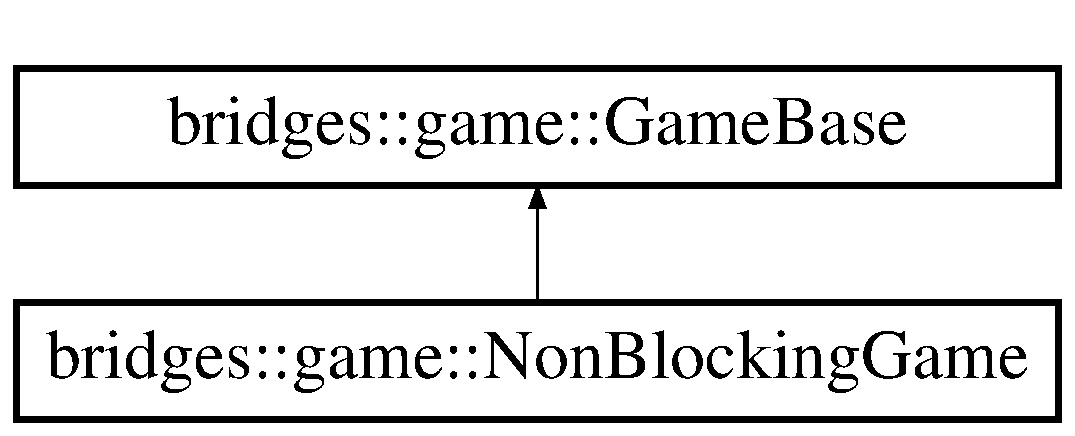
\includegraphics[height=2.000000cm]{classbridges_1_1game_1_1_game_base}
\end{center}
\end{figure}
\subsection*{Protected Member Functions}
\begin{DoxyCompactItemize}
\item 
\mbox{\hyperlink{classbridges_1_1game_1_1_game_base_abd73825c57a10d28191a3f1162eb9bd8}{Game\+Base}} (int assignment\+ID, std\+::string username, std\+::string apikey, int nb\+Row=10, int nb\+Column=10)
\item 
virtual void \mbox{\hyperlink{classbridges_1_1game_1_1_game_base_a9b6eb6fa7fceaac09d204b549164037f}{initialize}} ()=0
\begin{DoxyCompactList}\small\item\em This function is called once when the game starts. \end{DoxyCompactList}\item 
virtual void \mbox{\hyperlink{classbridges_1_1game_1_1_game_base_a16fb787bc65be1a582cddcfba3a0c5bb}{game\+Loop}} ()=0
\begin{DoxyCompactList}\small\item\em This function is called once per frame of the game. \end{DoxyCompactList}\item 
void \mbox{\hyperlink{classbridges_1_1game_1_1_game_base_a9612e74fe407127cae8455a0e34b5662}{register\+Key\+Listener}} (\mbox{\hyperlink{classbridges_1_1game_1_1_keypress_listener}{Keypress\+Listener}} $\ast$\mbox{\hyperlink{namespacebridges_1_1game_ab9a19c7ab6e2ebac2f95180e21733487a83878c91171338902e0fe0fb97a8c47a}{p}})
\begin{DoxyCompactList}\small\item\em register a new \mbox{\hyperlink{classbridges_1_1game_1_1_keypress_listener}{Keypress\+Listener}} \end{DoxyCompactList}\item 
void \mbox{\hyperlink{classbridges_1_1game_1_1_game_base_ac042479b1d1cf87b8ea7c8884d5326b6}{render}} ()
\begin{DoxyCompactList}\small\item\em Renders the game. \end{DoxyCompactList}\item 
bool \mbox{\hyperlink{classbridges_1_1game_1_1_game_base_adbc9759ea7995f2ee224e9b85d798f2f}{gameover}} () const
\item 
void \mbox{\hyperlink{classbridges_1_1game_1_1_game_base_a78d8bdc86cf7c5aba6a75879be1b6140}{quit}} ()
\begin{DoxyCompactList}\small\item\em calling this function causes the game to end. \end{DoxyCompactList}\item 
void \mbox{\hyperlink{classbridges_1_1game_1_1_game_base_ab667bbca1c81e5fb3aa8d81d70fe8cd2}{set\+B\+G\+Color}} (int row, int col, \mbox{\hyperlink{namespacebridges_1_1game_afaa832a4322b25b6a4ebfba832f10f26}{Named\+Color}} nc)
\begin{DoxyCompactList}\small\item\em Change the background color of a cell. \end{DoxyCompactList}\item 
void \mbox{\hyperlink{classbridges_1_1game_1_1_game_base_a415fa8f70bef364dfa966f2a86048901}{draw\+Symbol}} (int row, int col, \mbox{\hyperlink{namespacebridges_1_1game_ab9a19c7ab6e2ebac2f95180e21733487}{Named\+Symbol}} symb, \mbox{\hyperlink{namespacebridges_1_1game_afaa832a4322b25b6a4ebfba832f10f26}{Named\+Color}} nc)
\begin{DoxyCompactList}\small\item\em Draw an object on the game. \end{DoxyCompactList}\item 
void \mbox{\hyperlink{classbridges_1_1game_1_1_game_base_a108c2e3050a4d3f3af9950434e97102a}{set\+Title}} (std\+::string title)
\begin{DoxyCompactList}\small\item\em Set the title of the game. \end{DoxyCompactList}\item 
void \mbox{\hyperlink{classbridges_1_1game_1_1_game_base_ab490d78e11e4117c3a4915c78afa0973}{set\+Description}} (std\+::string desc)
\begin{DoxyCompactList}\small\item\em Set a short description of the game. \end{DoxyCompactList}\item 
\mbox{\hyperlink{namespacebridges_1_1game_afaa832a4322b25b6a4ebfba832f10f26}{Named\+Color}} \mbox{\hyperlink{classbridges_1_1game_1_1_game_base_a924f911774a89d18ccb391bb28fd703c}{get\+B\+G\+Color}} (int row, int col)
\begin{DoxyCompactList}\small\item\em What color is this cell? \end{DoxyCompactList}\item 
\mbox{\hyperlink{namespacebridges_1_1game_ab9a19c7ab6e2ebac2f95180e21733487}{Named\+Symbol}} \mbox{\hyperlink{classbridges_1_1game_1_1_game_base_a0dfec715b0ed49c37b4b6689f2470b25}{get\+Symbol}} (int row, int col)
\begin{DoxyCompactList}\small\item\em What object is in this cell? \end{DoxyCompactList}\item 
\mbox{\hyperlink{namespacebridges_1_1game_afaa832a4322b25b6a4ebfba832f10f26}{Named\+Color}} \mbox{\hyperlink{classbridges_1_1game_1_1_game_base_a26c9f9547cc6f992a829ce5d6edd8f85}{get\+Symbol\+Color}} (int row, int col)
\begin{DoxyCompactList}\small\item\em What color is object in this cell? \end{DoxyCompactList}\item 
int \mbox{\hyperlink{classbridges_1_1game_1_1_game_base_ad74bf992cced25e9997fbf8a63bf8157}{get\+Board\+Width}} ()
\begin{DoxyCompactList}\small\item\em How wide is the Game Board? \end{DoxyCompactList}\item 
int \mbox{\hyperlink{classbridges_1_1game_1_1_game_base_a14510d6685e0b224c8995e397ad64adc}{get\+Board\+Height}} ()
\begin{DoxyCompactList}\small\item\em How tall is the Game Board? \end{DoxyCompactList}\end{DoxyCompactItemize}
\subsection*{Protected Attributes}
\begin{DoxyCompactItemize}
\item 
bool \mbox{\hyperlink{classbridges_1_1game_1_1_game_base_ad2af01edd927a31613d3b881286541bb}{debug}} = false
\end{DoxyCompactItemize}


\subsection{Constructor \& Destructor Documentation}
\mbox{\Hypertarget{classbridges_1_1game_1_1_game_base_abd73825c57a10d28191a3f1162eb9bd8}\label{classbridges_1_1game_1_1_game_base_abd73825c57a10d28191a3f1162eb9bd8}} 
\index{bridges::game::GameBase@{bridges::game::GameBase}!GameBase@{GameBase}}
\index{GameBase@{GameBase}!bridges::game::GameBase@{bridges::game::GameBase}}
\subsubsection{\texorpdfstring{GameBase()}{GameBase()}}
{\footnotesize\ttfamily bridges\+::game\+::\+Game\+Base\+::\+Game\+Base (\begin{DoxyParamCaption}\item[{int}]{assignment\+ID,  }\item[{std\+::string}]{username,  }\item[{std\+::string}]{apikey,  }\item[{int}]{nb\+Row = {\ttfamily 10},  }\item[{int}]{nb\+Column = {\ttfamily 10} }\end{DoxyParamCaption})\hspace{0.3cm}{\ttfamily [inline]}, {\ttfamily [protected]}}

Having a protected constructor prevent the object from being directly created. Since \mbox{\hyperlink{classbridges_1_1game_1_1_game_base}{Game\+Base}} is meant to be a purely internal class, that seems appropriate. 

\subsection{Member Function Documentation}
\mbox{\Hypertarget{classbridges_1_1game_1_1_game_base_a415fa8f70bef364dfa966f2a86048901}\label{classbridges_1_1game_1_1_game_base_a415fa8f70bef364dfa966f2a86048901}} 
\index{bridges::game::GameBase@{bridges::game::GameBase}!drawSymbol@{drawSymbol}}
\index{drawSymbol@{drawSymbol}!bridges::game::GameBase@{bridges::game::GameBase}}
\subsubsection{\texorpdfstring{drawSymbol()}{drawSymbol()}}
{\footnotesize\ttfamily void bridges\+::game\+::\+Game\+Base\+::draw\+Symbol (\begin{DoxyParamCaption}\item[{int}]{row,  }\item[{int}]{col,  }\item[{\mbox{\hyperlink{namespacebridges_1_1game_ab9a19c7ab6e2ebac2f95180e21733487}{Named\+Symbol}}}]{symb,  }\item[{\mbox{\hyperlink{namespacebridges_1_1game_afaa832a4322b25b6a4ebfba832f10f26}{Named\+Color}}}]{nc }\end{DoxyParamCaption})\hspace{0.3cm}{\ttfamily [inline]}, {\ttfamily [protected]}}



Draw an object on the game. 


\begin{DoxyParams}{Parameters}
{\em row} & row of the cell to draw the object on \\
\hline
{\em col} & column of the cell to draw the object on \\
\hline
{\em symb} & symbol representing the object \\
\hline
{\em nc} & color of the object \\
\hline
\end{DoxyParams}
\mbox{\Hypertarget{classbridges_1_1game_1_1_game_base_a16fb787bc65be1a582cddcfba3a0c5bb}\label{classbridges_1_1game_1_1_game_base_a16fb787bc65be1a582cddcfba3a0c5bb}} 
\index{bridges::game::GameBase@{bridges::game::GameBase}!gameLoop@{gameLoop}}
\index{gameLoop@{gameLoop}!bridges::game::GameBase@{bridges::game::GameBase}}
\subsubsection{\texorpdfstring{gameLoop()}{gameLoop()}}
{\footnotesize\ttfamily virtual void bridges\+::game\+::\+Game\+Base\+::game\+Loop (\begin{DoxyParamCaption}{ }\end{DoxyParamCaption})\hspace{0.3cm}{\ttfamily [protected]}, {\ttfamily [pure virtual]}}



This function is called once per frame of the game. 

Students write this function. It will be called at each frame of the game. \mbox{\Hypertarget{classbridges_1_1game_1_1_game_base_adbc9759ea7995f2ee224e9b85d798f2f}\label{classbridges_1_1game_1_1_game_base_adbc9759ea7995f2ee224e9b85d798f2f}} 
\index{bridges::game::GameBase@{bridges::game::GameBase}!gameover@{gameover}}
\index{gameover@{gameover}!bridges::game::GameBase@{bridges::game::GameBase}}
\subsubsection{\texorpdfstring{gameover()}{gameover()}}
{\footnotesize\ttfamily bool bridges\+::game\+::\+Game\+Base\+::gameover (\begin{DoxyParamCaption}{ }\end{DoxyParamCaption}) const\hspace{0.3cm}{\ttfamily [inline]}, {\ttfamily [protected]}}

\mbox{\Hypertarget{classbridges_1_1game_1_1_game_base_a924f911774a89d18ccb391bb28fd703c}\label{classbridges_1_1game_1_1_game_base_a924f911774a89d18ccb391bb28fd703c}} 
\index{bridges::game::GameBase@{bridges::game::GameBase}!getBGColor@{getBGColor}}
\index{getBGColor@{getBGColor}!bridges::game::GameBase@{bridges::game::GameBase}}
\subsubsection{\texorpdfstring{getBGColor()}{getBGColor()}}
{\footnotesize\ttfamily \mbox{\hyperlink{namespacebridges_1_1game_afaa832a4322b25b6a4ebfba832f10f26}{Named\+Color}} bridges\+::game\+::\+Game\+Base\+::get\+B\+G\+Color (\begin{DoxyParamCaption}\item[{int}]{row,  }\item[{int}]{col }\end{DoxyParamCaption})\hspace{0.3cm}{\ttfamily [inline]}, {\ttfamily [protected]}}



What color is this cell? 


\begin{DoxyParams}{Parameters}
{\em row} & row of the cell \\
\hline
{\em col} & column of the cell \\
\hline
\end{DoxyParams}
\mbox{\Hypertarget{classbridges_1_1game_1_1_game_base_a14510d6685e0b224c8995e397ad64adc}\label{classbridges_1_1game_1_1_game_base_a14510d6685e0b224c8995e397ad64adc}} 
\index{bridges::game::GameBase@{bridges::game::GameBase}!getBoardHeight@{getBoardHeight}}
\index{getBoardHeight@{getBoardHeight}!bridges::game::GameBase@{bridges::game::GameBase}}
\subsubsection{\texorpdfstring{getBoardHeight()}{getBoardHeight()}}
{\footnotesize\ttfamily int bridges\+::game\+::\+Game\+Base\+::get\+Board\+Height (\begin{DoxyParamCaption}{ }\end{DoxyParamCaption})\hspace{0.3cm}{\ttfamily [inline]}, {\ttfamily [protected]}}



How tall is the Game Board? 

\begin{DoxyReturn}{Returns}
the number of rows of the board 
\end{DoxyReturn}
\mbox{\Hypertarget{classbridges_1_1game_1_1_game_base_ad74bf992cced25e9997fbf8a63bf8157}\label{classbridges_1_1game_1_1_game_base_ad74bf992cced25e9997fbf8a63bf8157}} 
\index{bridges::game::GameBase@{bridges::game::GameBase}!getBoardWidth@{getBoardWidth}}
\index{getBoardWidth@{getBoardWidth}!bridges::game::GameBase@{bridges::game::GameBase}}
\subsubsection{\texorpdfstring{getBoardWidth()}{getBoardWidth()}}
{\footnotesize\ttfamily int bridges\+::game\+::\+Game\+Base\+::get\+Board\+Width (\begin{DoxyParamCaption}{ }\end{DoxyParamCaption})\hspace{0.3cm}{\ttfamily [inline]}, {\ttfamily [protected]}}



How wide is the Game Board? 

\begin{DoxyReturn}{Returns}
the number of columns of the board 
\end{DoxyReturn}
\mbox{\Hypertarget{classbridges_1_1game_1_1_game_base_a0dfec715b0ed49c37b4b6689f2470b25}\label{classbridges_1_1game_1_1_game_base_a0dfec715b0ed49c37b4b6689f2470b25}} 
\index{bridges::game::GameBase@{bridges::game::GameBase}!getSymbol@{getSymbol}}
\index{getSymbol@{getSymbol}!bridges::game::GameBase@{bridges::game::GameBase}}
\subsubsection{\texorpdfstring{getSymbol()}{getSymbol()}}
{\footnotesize\ttfamily \mbox{\hyperlink{namespacebridges_1_1game_ab9a19c7ab6e2ebac2f95180e21733487}{Named\+Symbol}} bridges\+::game\+::\+Game\+Base\+::get\+Symbol (\begin{DoxyParamCaption}\item[{int}]{row,  }\item[{int}]{col }\end{DoxyParamCaption})\hspace{0.3cm}{\ttfamily [inline]}, {\ttfamily [protected]}}



What object is in this cell? 


\begin{DoxyParams}{Parameters}
{\em row} & row of the cell \\
\hline
{\em col} & column of the cell \\
\hline
\end{DoxyParams}
\mbox{\Hypertarget{classbridges_1_1game_1_1_game_base_a26c9f9547cc6f992a829ce5d6edd8f85}\label{classbridges_1_1game_1_1_game_base_a26c9f9547cc6f992a829ce5d6edd8f85}} 
\index{bridges::game::GameBase@{bridges::game::GameBase}!getSymbolColor@{getSymbolColor}}
\index{getSymbolColor@{getSymbolColor}!bridges::game::GameBase@{bridges::game::GameBase}}
\subsubsection{\texorpdfstring{getSymbolColor()}{getSymbolColor()}}
{\footnotesize\ttfamily \mbox{\hyperlink{namespacebridges_1_1game_afaa832a4322b25b6a4ebfba832f10f26}{Named\+Color}} bridges\+::game\+::\+Game\+Base\+::get\+Symbol\+Color (\begin{DoxyParamCaption}\item[{int}]{row,  }\item[{int}]{col }\end{DoxyParamCaption})\hspace{0.3cm}{\ttfamily [inline]}, {\ttfamily [protected]}}



What color is object in this cell? 


\begin{DoxyParams}{Parameters}
{\em row} & row of the cell \\
\hline
{\em col} & column of the cell \\
\hline
\end{DoxyParams}
\mbox{\Hypertarget{classbridges_1_1game_1_1_game_base_a9b6eb6fa7fceaac09d204b549164037f}\label{classbridges_1_1game_1_1_game_base_a9b6eb6fa7fceaac09d204b549164037f}} 
\index{bridges::game::GameBase@{bridges::game::GameBase}!initialize@{initialize}}
\index{initialize@{initialize}!bridges::game::GameBase@{bridges::game::GameBase}}
\subsubsection{\texorpdfstring{initialize()}{initialize()}}
{\footnotesize\ttfamily virtual void bridges\+::game\+::\+Game\+Base\+::initialize (\begin{DoxyParamCaption}{ }\end{DoxyParamCaption})\hspace{0.3cm}{\ttfamily [protected]}, {\ttfamily [pure virtual]}}



This function is called once when the game starts. 

Students write this function. It will be called once at the begining of the game. \mbox{\Hypertarget{classbridges_1_1game_1_1_game_base_a78d8bdc86cf7c5aba6a75879be1b6140}\label{classbridges_1_1game_1_1_game_base_a78d8bdc86cf7c5aba6a75879be1b6140}} 
\index{bridges::game::GameBase@{bridges::game::GameBase}!quit@{quit}}
\index{quit@{quit}!bridges::game::GameBase@{bridges::game::GameBase}}
\subsubsection{\texorpdfstring{quit()}{quit()}}
{\footnotesize\ttfamily void bridges\+::game\+::\+Game\+Base\+::quit (\begin{DoxyParamCaption}{ }\end{DoxyParamCaption})\hspace{0.3cm}{\ttfamily [inline]}, {\ttfamily [protected]}}



calling this function causes the game to end. 

That is to say, the current frame will be the last frame of the game. \mbox{\Hypertarget{classbridges_1_1game_1_1_game_base_a9612e74fe407127cae8455a0e34b5662}\label{classbridges_1_1game_1_1_game_base_a9612e74fe407127cae8455a0e34b5662}} 
\index{bridges::game::GameBase@{bridges::game::GameBase}!registerKeyListener@{registerKeyListener}}
\index{registerKeyListener@{registerKeyListener}!bridges::game::GameBase@{bridges::game::GameBase}}
\subsubsection{\texorpdfstring{registerKeyListener()}{registerKeyListener()}}
{\footnotesize\ttfamily void bridges\+::game\+::\+Game\+Base\+::register\+Key\+Listener (\begin{DoxyParamCaption}\item[{\mbox{\hyperlink{classbridges_1_1game_1_1_keypress_listener}{Keypress\+Listener}} $\ast$}]{p }\end{DoxyParamCaption})\hspace{0.3cm}{\ttfamily [inline]}, {\ttfamily [protected]}}



register a new \mbox{\hyperlink{classbridges_1_1game_1_1_keypress_listener}{Keypress\+Listener}} 

Students should not have to call this function directly. The \mbox{\hyperlink{classbridges_1_1game_1_1_keypress_listener}{Keypress\+Listener}} listener will get notified of all keypresses (up and down) that happens in the game.


\begin{DoxyParams}{Parameters}
{\em p} & a \mbox{\hyperlink{classbridges_1_1game_1_1_keypress_listener}{Keypress\+Listener}} to register \\
\hline
\end{DoxyParams}
\mbox{\Hypertarget{classbridges_1_1game_1_1_game_base_ac042479b1d1cf87b8ea7c8884d5326b6}\label{classbridges_1_1game_1_1_game_base_ac042479b1d1cf87b8ea7c8884d5326b6}} 
\index{bridges::game::GameBase@{bridges::game::GameBase}!render@{render}}
\index{render@{render}!bridges::game::GameBase@{bridges::game::GameBase}}
\subsubsection{\texorpdfstring{render()}{render()}}
{\footnotesize\ttfamily void bridges\+::game\+::\+Game\+Base\+::render (\begin{DoxyParamCaption}{ }\end{DoxyParamCaption})\hspace{0.3cm}{\ttfamily [inline]}, {\ttfamily [protected]}}



Renders the game. 

Student should not have to call this function directly. It is called automatically by \mbox{\hyperlink{classbridges_1_1_bridges}{Bridges}}. \mbox{\Hypertarget{classbridges_1_1game_1_1_game_base_ab667bbca1c81e5fb3aa8d81d70fe8cd2}\label{classbridges_1_1game_1_1_game_base_ab667bbca1c81e5fb3aa8d81d70fe8cd2}} 
\index{bridges::game::GameBase@{bridges::game::GameBase}!setBGColor@{setBGColor}}
\index{setBGColor@{setBGColor}!bridges::game::GameBase@{bridges::game::GameBase}}
\subsubsection{\texorpdfstring{setBGColor()}{setBGColor()}}
{\footnotesize\ttfamily void bridges\+::game\+::\+Game\+Base\+::set\+B\+G\+Color (\begin{DoxyParamCaption}\item[{int}]{row,  }\item[{int}]{col,  }\item[{\mbox{\hyperlink{namespacebridges_1_1game_afaa832a4322b25b6a4ebfba832f10f26}{Named\+Color}}}]{nc }\end{DoxyParamCaption})\hspace{0.3cm}{\ttfamily [inline]}, {\ttfamily [protected]}}



Change the background color of a cell. 


\begin{DoxyParams}{Parameters}
{\em row} & row of the cell to set \\
\hline
{\em col} & column of the cell to set \\
\hline
{\em nc} & Named\+Color to set \\
\hline
\end{DoxyParams}
\mbox{\Hypertarget{classbridges_1_1game_1_1_game_base_ab490d78e11e4117c3a4915c78afa0973}\label{classbridges_1_1game_1_1_game_base_ab490d78e11e4117c3a4915c78afa0973}} 
\index{bridges::game::GameBase@{bridges::game::GameBase}!setDescription@{setDescription}}
\index{setDescription@{setDescription}!bridges::game::GameBase@{bridges::game::GameBase}}
\subsubsection{\texorpdfstring{setDescription()}{setDescription()}}
{\footnotesize\ttfamily void bridges\+::game\+::\+Game\+Base\+::set\+Description (\begin{DoxyParamCaption}\item[{std\+::string}]{desc }\end{DoxyParamCaption})\hspace{0.3cm}{\ttfamily [inline]}, {\ttfamily [protected]}}



Set a short description of the game. 


\begin{DoxyParams}{Parameters}
{\em desc} & Description of the game \\
\hline
\end{DoxyParams}
\mbox{\Hypertarget{classbridges_1_1game_1_1_game_base_a108c2e3050a4d3f3af9950434e97102a}\label{classbridges_1_1game_1_1_game_base_a108c2e3050a4d3f3af9950434e97102a}} 
\index{bridges::game::GameBase@{bridges::game::GameBase}!setTitle@{setTitle}}
\index{setTitle@{setTitle}!bridges::game::GameBase@{bridges::game::GameBase}}
\subsubsection{\texorpdfstring{setTitle()}{setTitle()}}
{\footnotesize\ttfamily void bridges\+::game\+::\+Game\+Base\+::set\+Title (\begin{DoxyParamCaption}\item[{std\+::string}]{title }\end{DoxyParamCaption})\hspace{0.3cm}{\ttfamily [inline]}, {\ttfamily [protected]}}



Set the title of the game. 


\begin{DoxyParams}{Parameters}
{\em title} & Title of the game \\
\hline
\end{DoxyParams}


\subsection{Member Data Documentation}
\mbox{\Hypertarget{classbridges_1_1game_1_1_game_base_ad2af01edd927a31613d3b881286541bb}\label{classbridges_1_1game_1_1_game_base_ad2af01edd927a31613d3b881286541bb}} 
\index{bridges::game::GameBase@{bridges::game::GameBase}!debug@{debug}}
\index{debug@{debug}!bridges::game::GameBase@{bridges::game::GameBase}}
\subsubsection{\texorpdfstring{debug}{debug}}
{\footnotesize\ttfamily bool bridges\+::game\+::\+Game\+Base\+::debug = false\hspace{0.3cm}{\ttfamily [protected]}}



The documentation for this class was generated from the following file\+:\begin{DoxyCompactItemize}
\item 
/\+Users/kalpathi/gr/bridges/cxx/src/\mbox{\hyperlink{_game_base_8h}{Game\+Base.\+h}}\end{DoxyCompactItemize}

\hypertarget{classbridges_1_1game_1_1_game_cell}{}\section{bridges\+::game\+::Game\+Cell Class Reference}
\label{classbridges_1_1game_1_1_game_cell}\index{bridges::game::GameCell@{bridges::game::GameCell}}


{\ttfamily \#include $<$Game\+Grid.\+h$>$}

\subsection*{Public Member Functions}
\begin{DoxyCompactItemize}
\item 
\mbox{\hyperlink{classbridges_1_1game_1_1_game_cell_a750114853f2f0f7519cb663352230868}{Game\+Cell}} ()
\item 
\mbox{\hyperlink{classbridges_1_1game_1_1_game_cell_a743b618fc8553aa9aac33ddc3bb65a79}{Game\+Cell}} (\mbox{\hyperlink{namespacebridges_1_1game_afaa832a4322b25b6a4ebfba832f10f26}{Named\+Color}} bg, \mbox{\hyperlink{namespacebridges_1_1game_afaa832a4322b25b6a4ebfba832f10f26}{Named\+Color}} fg, \mbox{\hyperlink{namespacebridges_1_1game_ab9a19c7ab6e2ebac2f95180e21733487}{Named\+Symbol}} symbol)
\item 
void \mbox{\hyperlink{classbridges_1_1game_1_1_game_cell_ac2ee6a35500564b3df970551dcf56892}{set\+B\+G\+Color}} (\mbox{\hyperlink{namespacebridges_1_1game_afaa832a4322b25b6a4ebfba832f10f26}{Named\+Color}} bg)
\item 
void \mbox{\hyperlink{classbridges_1_1game_1_1_game_cell_a899b56c1561ca4acacc42e9d740aa19a}{set\+F\+G\+Color}} (\mbox{\hyperlink{namespacebridges_1_1game_afaa832a4322b25b6a4ebfba832f10f26}{Named\+Color}} fg)
\item 
void \mbox{\hyperlink{classbridges_1_1game_1_1_game_cell_abd0dde526adf160bf5d026e24410645a}{set\+Symbol}} (\mbox{\hyperlink{namespacebridges_1_1game_ab9a19c7ab6e2ebac2f95180e21733487}{Named\+Symbol}} \mbox{\hyperlink{namespacebridges_1_1game_ab9a19c7ab6e2ebac2f95180e21733487a03c7c0ace395d80182db07ae2c30f034}{s}})
\item 
\mbox{\hyperlink{namespacebridges_1_1game_afaa832a4322b25b6a4ebfba832f10f26}{Named\+Color}} \mbox{\hyperlink{classbridges_1_1game_1_1_game_cell_abfe53785cb331ee73455ef4f7c2f1ba6}{get\+B\+G\+Color}} () const
\item 
\mbox{\hyperlink{namespacebridges_1_1game_afaa832a4322b25b6a4ebfba832f10f26}{Named\+Color}} \mbox{\hyperlink{classbridges_1_1game_1_1_game_cell_af9269057618ffdd503768ccd6b6e6f56}{get\+F\+G\+Color}} () const
\item 
\mbox{\hyperlink{namespacebridges_1_1game_ab9a19c7ab6e2ebac2f95180e21733487}{Named\+Symbol}} \mbox{\hyperlink{classbridges_1_1game_1_1_game_cell_a55ed5769afe548a707117379425613f0}{get\+Symbol}} () const
\end{DoxyCompactItemize}


\subsection{Constructor \& Destructor Documentation}
\mbox{\Hypertarget{classbridges_1_1game_1_1_game_cell_a750114853f2f0f7519cb663352230868}\label{classbridges_1_1game_1_1_game_cell_a750114853f2f0f7519cb663352230868}} 
\index{bridges::game::GameCell@{bridges::game::GameCell}!GameCell@{GameCell}}
\index{GameCell@{GameCell}!bridges::game::GameCell@{bridges::game::GameCell}}
\subsubsection{\texorpdfstring{GameCell()}{GameCell()}\hspace{0.1cm}{\footnotesize\ttfamily [1/2]}}
{\footnotesize\ttfamily bridges\+::game\+::\+Game\+Cell\+::\+Game\+Cell (\begin{DoxyParamCaption}{ }\end{DoxyParamCaption})\hspace{0.3cm}{\ttfamily [inline]}}

\mbox{\Hypertarget{classbridges_1_1game_1_1_game_cell_a743b618fc8553aa9aac33ddc3bb65a79}\label{classbridges_1_1game_1_1_game_cell_a743b618fc8553aa9aac33ddc3bb65a79}} 
\index{bridges::game::GameCell@{bridges::game::GameCell}!GameCell@{GameCell}}
\index{GameCell@{GameCell}!bridges::game::GameCell@{bridges::game::GameCell}}
\subsubsection{\texorpdfstring{GameCell()}{GameCell()}\hspace{0.1cm}{\footnotesize\ttfamily [2/2]}}
{\footnotesize\ttfamily bridges\+::game\+::\+Game\+Cell\+::\+Game\+Cell (\begin{DoxyParamCaption}\item[{\mbox{\hyperlink{namespacebridges_1_1game_afaa832a4322b25b6a4ebfba832f10f26}{Named\+Color}}}]{bg,  }\item[{\mbox{\hyperlink{namespacebridges_1_1game_afaa832a4322b25b6a4ebfba832f10f26}{Named\+Color}}}]{fg,  }\item[{\mbox{\hyperlink{namespacebridges_1_1game_ab9a19c7ab6e2ebac2f95180e21733487}{Named\+Symbol}}}]{symbol }\end{DoxyParamCaption})\hspace{0.3cm}{\ttfamily [inline]}}



\subsection{Member Function Documentation}
\mbox{\Hypertarget{classbridges_1_1game_1_1_game_cell_abfe53785cb331ee73455ef4f7c2f1ba6}\label{classbridges_1_1game_1_1_game_cell_abfe53785cb331ee73455ef4f7c2f1ba6}} 
\index{bridges::game::GameCell@{bridges::game::GameCell}!getBGColor@{getBGColor}}
\index{getBGColor@{getBGColor}!bridges::game::GameCell@{bridges::game::GameCell}}
\subsubsection{\texorpdfstring{getBGColor()}{getBGColor()}}
{\footnotesize\ttfamily \mbox{\hyperlink{namespacebridges_1_1game_afaa832a4322b25b6a4ebfba832f10f26}{Named\+Color}} bridges\+::game\+::\+Game\+Cell\+::get\+B\+G\+Color (\begin{DoxyParamCaption}{ }\end{DoxyParamCaption}) const\hspace{0.3cm}{\ttfamily [inline]}}

\mbox{\Hypertarget{classbridges_1_1game_1_1_game_cell_af9269057618ffdd503768ccd6b6e6f56}\label{classbridges_1_1game_1_1_game_cell_af9269057618ffdd503768ccd6b6e6f56}} 
\index{bridges::game::GameCell@{bridges::game::GameCell}!getFGColor@{getFGColor}}
\index{getFGColor@{getFGColor}!bridges::game::GameCell@{bridges::game::GameCell}}
\subsubsection{\texorpdfstring{getFGColor()}{getFGColor()}}
{\footnotesize\ttfamily \mbox{\hyperlink{namespacebridges_1_1game_afaa832a4322b25b6a4ebfba832f10f26}{Named\+Color}} bridges\+::game\+::\+Game\+Cell\+::get\+F\+G\+Color (\begin{DoxyParamCaption}{ }\end{DoxyParamCaption}) const\hspace{0.3cm}{\ttfamily [inline]}}

\mbox{\Hypertarget{classbridges_1_1game_1_1_game_cell_a55ed5769afe548a707117379425613f0}\label{classbridges_1_1game_1_1_game_cell_a55ed5769afe548a707117379425613f0}} 
\index{bridges::game::GameCell@{bridges::game::GameCell}!getSymbol@{getSymbol}}
\index{getSymbol@{getSymbol}!bridges::game::GameCell@{bridges::game::GameCell}}
\subsubsection{\texorpdfstring{getSymbol()}{getSymbol()}}
{\footnotesize\ttfamily \mbox{\hyperlink{namespacebridges_1_1game_ab9a19c7ab6e2ebac2f95180e21733487}{Named\+Symbol}} bridges\+::game\+::\+Game\+Cell\+::get\+Symbol (\begin{DoxyParamCaption}{ }\end{DoxyParamCaption}) const\hspace{0.3cm}{\ttfamily [inline]}}

\mbox{\Hypertarget{classbridges_1_1game_1_1_game_cell_ac2ee6a35500564b3df970551dcf56892}\label{classbridges_1_1game_1_1_game_cell_ac2ee6a35500564b3df970551dcf56892}} 
\index{bridges::game::GameCell@{bridges::game::GameCell}!setBGColor@{setBGColor}}
\index{setBGColor@{setBGColor}!bridges::game::GameCell@{bridges::game::GameCell}}
\subsubsection{\texorpdfstring{setBGColor()}{setBGColor()}}
{\footnotesize\ttfamily void bridges\+::game\+::\+Game\+Cell\+::set\+B\+G\+Color (\begin{DoxyParamCaption}\item[{\mbox{\hyperlink{namespacebridges_1_1game_afaa832a4322b25b6a4ebfba832f10f26}{Named\+Color}}}]{bg }\end{DoxyParamCaption})\hspace{0.3cm}{\ttfamily [inline]}}

Set background color using Named\+Color Enum argument 
\begin{DoxyParams}{Parameters}
{\em bg} & -\/ Named Color from the Named\+Color enum \\
\hline
\end{DoxyParams}
\mbox{\Hypertarget{classbridges_1_1game_1_1_game_cell_a899b56c1561ca4acacc42e9d740aa19a}\label{classbridges_1_1game_1_1_game_cell_a899b56c1561ca4acacc42e9d740aa19a}} 
\index{bridges::game::GameCell@{bridges::game::GameCell}!setFGColor@{setFGColor}}
\index{setFGColor@{setFGColor}!bridges::game::GameCell@{bridges::game::GameCell}}
\subsubsection{\texorpdfstring{setFGColor()}{setFGColor()}}
{\footnotesize\ttfamily void bridges\+::game\+::\+Game\+Cell\+::set\+F\+G\+Color (\begin{DoxyParamCaption}\item[{\mbox{\hyperlink{namespacebridges_1_1game_afaa832a4322b25b6a4ebfba832f10f26}{Named\+Color}}}]{fg }\end{DoxyParamCaption})\hspace{0.3cm}{\ttfamily [inline]}}

Set foreground color using Named\+Color Enum argument 
\begin{DoxyParams}{Parameters}
{\em fg} & -\/ Named Color from the Named\+Color enum \\
\hline
\end{DoxyParams}
\mbox{\Hypertarget{classbridges_1_1game_1_1_game_cell_abd0dde526adf160bf5d026e24410645a}\label{classbridges_1_1game_1_1_game_cell_abd0dde526adf160bf5d026e24410645a}} 
\index{bridges::game::GameCell@{bridges::game::GameCell}!setSymbol@{setSymbol}}
\index{setSymbol@{setSymbol}!bridges::game::GameCell@{bridges::game::GameCell}}
\subsubsection{\texorpdfstring{setSymbol()}{setSymbol()}}
{\footnotesize\ttfamily void bridges\+::game\+::\+Game\+Cell\+::set\+Symbol (\begin{DoxyParamCaption}\item[{\mbox{\hyperlink{namespacebridges_1_1game_ab9a19c7ab6e2ebac2f95180e21733487}{Named\+Symbol}}}]{s }\end{DoxyParamCaption})\hspace{0.3cm}{\ttfamily [inline]}}

Set symbol using int argument 
\begin{DoxyParams}{Parameters}
{\em s} & -\/ Named symbol \\
\hline
\end{DoxyParams}


The documentation for this class was generated from the following file\+:\begin{DoxyCompactItemize}
\item 
/\+Users/kalpathi/gr/bridges/cxx/src/\mbox{\hyperlink{_game_grid_8h}{Game\+Grid.\+h}}\end{DoxyCompactItemize}

\hypertarget{classbridges_1_1game_1_1_game_grid}{}\section{bridges\+:\+:game\+:\+:Game\+Grid Class Reference}
\label{classbridges_1_1game_1_1_game_grid}\index{bridges\+::game\+::\+Game\+Grid@{bridges\+::game\+::\+Game\+Grid}}


{\ttfamily \#include $<$Game\+Grid.\+h$>$}

Inheritance diagram for bridges\+:\+:game\+:\+:Game\+Grid\+:\begin{figure}[H]
\begin{center}
\leavevmode
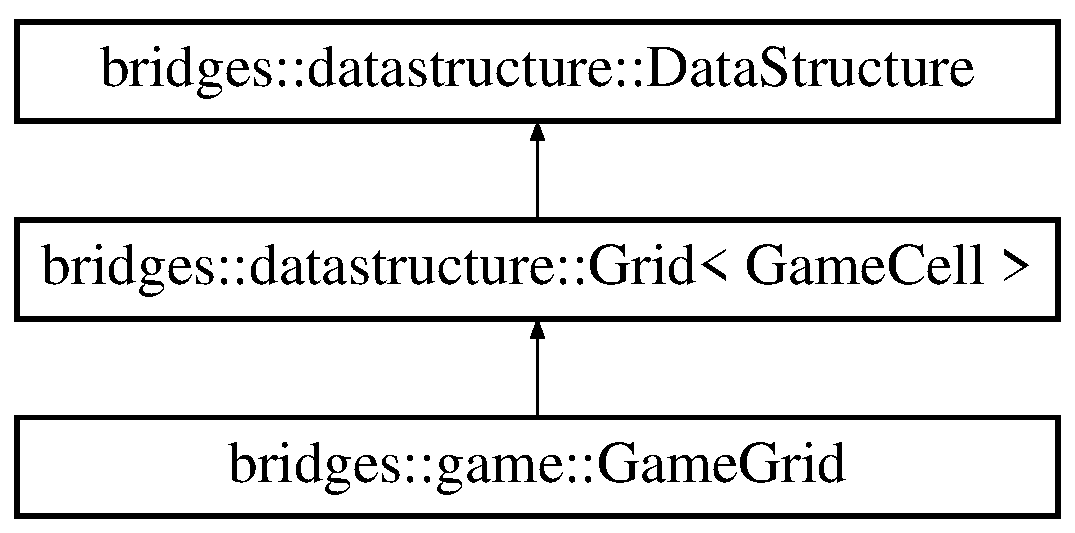
\includegraphics[height=3.000000cm]{classbridges_1_1game_1_1_game_grid}
\end{center}
\end{figure}


\subsection{Detailed Description}
This is a class in B\+R\+I\+D\+G\+ES for representing an (n x n)game grid. 

This class is part of the \hyperlink{classbridges_1_1_bridges}{Bridges} Game A\+PI

\begin{DoxySeeAlso}{See also}
See the detailed \hyperlink{classbridges_1_1_bridges}{Bridges} \hyperlink{namespacebridges_1_1game}{game} tutorial for examples at \href{http://bridgesuncc.github.io/tutorials/NonBlockingGame.html}{\tt http\+://bridgesuncc.\+github.\+io/tutorials/\+Non\+Blocking\+Game.\+html}
\end{DoxySeeAlso}
\begin{DoxyAuthor}{Author}
Erik Saule, 
\end{DoxyAuthor}
\begin{DoxyDate}{Date}
2018, 2019, 12/28/20 
\end{DoxyDate}
\subsection*{Public Member Functions}
\begin{DoxyCompactItemize}
\item 
void \hyperlink{classbridges_1_1game_1_1_game_grid_a141dbed75aeb34498ee0f8ad17c2cb6c}{set\+B\+G\+Color} (int row, int col, \hyperlink{namespacebridges_1_1game_afaa832a4322b25b6a4ebfba832f10f26}{Named\+Color} color)
\item 
\hyperlink{namespacebridges_1_1game_afaa832a4322b25b6a4ebfba832f10f26}{Named\+Color} \hyperlink{classbridges_1_1game_1_1_game_grid_ae63280e78a80eb0fe72050afa8ef2a63}{get\+B\+G\+Color} (int row, int col) const
\item 
\hyperlink{namespacebridges_1_1game_afaa832a4322b25b6a4ebfba832f10f26}{Named\+Color} \hyperlink{classbridges_1_1game_1_1_game_grid_a6d38c8ac0d4ccbdd1b2b1c5d2f445d9a}{get\+F\+G\+Color} (int row, int col) const
\item 
\hyperlink{namespacebridges_1_1game_ab9a19c7ab6e2ebac2f95180e21733487}{Named\+Symbol} \hyperlink{classbridges_1_1game_1_1_game_grid_aac18709133e1e2e6e77708779cabc553}{get\+Symbol} (int row, int col) const
\item 
void \hyperlink{classbridges_1_1game_1_1_game_grid_add272657d570437edc849eb7cfd061fb}{set\+F\+G\+Color} (int row, int col, \hyperlink{namespacebridges_1_1game_afaa832a4322b25b6a4ebfba832f10f26}{Named\+Color} color)
\item 
void \hyperlink{classbridges_1_1game_1_1_game_grid_aaca03d00599251edb5312e9ba51dd62e}{set\+Symbol} (int row, int col, \hyperlink{namespacebridges_1_1game_ab9a19c7ab6e2ebac2f95180e21733487}{Named\+Symbol} symbol)
\item 
void \hyperlink{classbridges_1_1game_1_1_game_grid_a32c5c19c1dff8d50001d2aa57cbda70b}{draw\+Symbol} (int row, int col, \hyperlink{namespacebridges_1_1game_ab9a19c7ab6e2ebac2f95180e21733487}{Named\+Symbol} symbol, \hyperlink{namespacebridges_1_1game_afaa832a4322b25b6a4ebfba832f10f26}{Named\+Color} color)
\item 
virtual const string \hyperlink{classbridges_1_1game_1_1_game_grid_a07da19700a077e3d0f2cde2cade2ba60}{get\+D\+Stype} () const override
\begin{DoxyCompactList}\small\item\em Return the data structure type. \end{DoxyCompactList}\item 
\hyperlink{classbridges_1_1game_1_1_game_grid_a00d0b39cd640fe338a96961ca1793191}{Game\+Grid} (int nbrow=10, int nbcol=10)
\item 
virtual const string \hyperlink{classbridges_1_1game_1_1_game_grid_aefbf4969375a174cefd8e2edf9fb6900}{get\+Data\+Structure\+Representation} () const override
\end{DoxyCompactItemize}
\subsection*{Additional Inherited Members}


\subsection{Constructor \& Destructor Documentation}
\mbox{\Hypertarget{classbridges_1_1game_1_1_game_grid_a00d0b39cd640fe338a96961ca1793191}\label{classbridges_1_1game_1_1_game_grid_a00d0b39cd640fe338a96961ca1793191}} 
\index{bridges\+::game\+::\+Game\+Grid@{bridges\+::game\+::\+Game\+Grid}!Game\+Grid@{Game\+Grid}}
\index{Game\+Grid@{Game\+Grid}!bridges\+::game\+::\+Game\+Grid@{bridges\+::game\+::\+Game\+Grid}}
\subsubsection{\texorpdfstring{Game\+Grid()}{GameGrid()}}
{\footnotesize\ttfamily bridges\+::game\+::\+Game\+Grid\+::\+Game\+Grid (\begin{DoxyParamCaption}\item[{int}]{nbrow = {\ttfamily 10},  }\item[{int}]{nbcol = {\ttfamily 10} }\end{DoxyParamCaption})\hspace{0.3cm}{\ttfamily [inline]}}

\hyperlink{classbridges_1_1game_1_1_game_grid}{Game\+Grid} constructors 

\subsection{Member Function Documentation}
\mbox{\Hypertarget{classbridges_1_1game_1_1_game_grid_a32c5c19c1dff8d50001d2aa57cbda70b}\label{classbridges_1_1game_1_1_game_grid_a32c5c19c1dff8d50001d2aa57cbda70b}} 
\index{bridges\+::game\+::\+Game\+Grid@{bridges\+::game\+::\+Game\+Grid}!draw\+Symbol@{draw\+Symbol}}
\index{draw\+Symbol@{draw\+Symbol}!bridges\+::game\+::\+Game\+Grid@{bridges\+::game\+::\+Game\+Grid}}
\subsubsection{\texorpdfstring{draw\+Symbol()}{drawSymbol()}}
{\footnotesize\ttfamily void bridges\+::game\+::\+Game\+Grid\+::draw\+Symbol (\begin{DoxyParamCaption}\item[{int}]{row,  }\item[{int}]{col,  }\item[{\hyperlink{namespacebridges_1_1game_ab9a19c7ab6e2ebac2f95180e21733487}{Named\+Symbol}}]{symbol,  }\item[{\hyperlink{namespacebridges_1_1game_afaa832a4322b25b6a4ebfba832f10f26}{Named\+Color}}]{color }\end{DoxyParamCaption})\hspace{0.3cm}{\ttfamily [inline]}}

Draw a symbol at the specified location 
\begin{DoxyParams}{Parameters}
{\em row,col} & -\/ integer indices specifying the position to modify \\
\hline
{\em symbol} & Symbol to draw \\
\hline
{\em color} & Color to draw the symbol in \\
\hline
\end{DoxyParams}
\mbox{\Hypertarget{classbridges_1_1game_1_1_game_grid_ae63280e78a80eb0fe72050afa8ef2a63}\label{classbridges_1_1game_1_1_game_grid_ae63280e78a80eb0fe72050afa8ef2a63}} 
\index{bridges\+::game\+::\+Game\+Grid@{bridges\+::game\+::\+Game\+Grid}!get\+B\+G\+Color@{get\+B\+G\+Color}}
\index{get\+B\+G\+Color@{get\+B\+G\+Color}!bridges\+::game\+::\+Game\+Grid@{bridges\+::game\+::\+Game\+Grid}}
\subsubsection{\texorpdfstring{get\+B\+G\+Color()}{getBGColor()}}
{\footnotesize\ttfamily \hyperlink{namespacebridges_1_1game_afaa832a4322b25b6a4ebfba832f10f26}{Named\+Color} bridges\+::game\+::\+Game\+Grid\+::get\+B\+G\+Color (\begin{DoxyParamCaption}\item[{int}]{row,  }\item[{int}]{col }\end{DoxyParamCaption}) const\hspace{0.3cm}{\ttfamily [inline]}}

\mbox{\Hypertarget{classbridges_1_1game_1_1_game_grid_aefbf4969375a174cefd8e2edf9fb6900}\label{classbridges_1_1game_1_1_game_grid_aefbf4969375a174cefd8e2edf9fb6900}} 
\index{bridges\+::game\+::\+Game\+Grid@{bridges\+::game\+::\+Game\+Grid}!get\+Data\+Structure\+Representation@{get\+Data\+Structure\+Representation}}
\index{get\+Data\+Structure\+Representation@{get\+Data\+Structure\+Representation}!bridges\+::game\+::\+Game\+Grid@{bridges\+::game\+::\+Game\+Grid}}
\subsubsection{\texorpdfstring{get\+Data\+Structure\+Representation()}{getDataStructureRepresentation()}}
{\footnotesize\ttfamily virtual const string bridges\+::game\+::\+Game\+Grid\+::get\+Data\+Structure\+Representation (\begin{DoxyParamCaption}{ }\end{DoxyParamCaption}) const\hspace{0.3cm}{\ttfamily [inline]}, {\ttfamily [override]}, {\ttfamily [virtual]}}

get the J\+S\+ON representation of the game grid

\begin{DoxyReturn}{Returns}
the J\+S\+ON representation of the game grid 
\end{DoxyReturn}


Implements \hyperlink{classbridges_1_1datastructure_1_1_data_structure}{bridges\+::datastructure\+::\+Data\+Structure}.

\mbox{\Hypertarget{classbridges_1_1game_1_1_game_grid_a07da19700a077e3d0f2cde2cade2ba60}\label{classbridges_1_1game_1_1_game_grid_a07da19700a077e3d0f2cde2cade2ba60}} 
\index{bridges\+::game\+::\+Game\+Grid@{bridges\+::game\+::\+Game\+Grid}!get\+D\+Stype@{get\+D\+Stype}}
\index{get\+D\+Stype@{get\+D\+Stype}!bridges\+::game\+::\+Game\+Grid@{bridges\+::game\+::\+Game\+Grid}}
\subsubsection{\texorpdfstring{get\+D\+Stype()}{getDStype()}}
{\footnotesize\ttfamily virtual const string bridges\+::game\+::\+Game\+Grid\+::get\+D\+Stype (\begin{DoxyParamCaption}{ }\end{DoxyParamCaption}) const\hspace{0.3cm}{\ttfamily [inline]}, {\ttfamily [override]}, {\ttfamily [virtual]}}



Return the data structure type. 

\begin{DoxyReturn}{Returns}
grid type (string) 
\end{DoxyReturn}


Reimplemented from \hyperlink{classbridges_1_1datastructure_1_1_grid_a16aeae38446b96f440dea15f2b19334d}{bridges\+::datastructure\+::\+Grid$<$ Game\+Cell $>$}.

\mbox{\Hypertarget{classbridges_1_1game_1_1_game_grid_a6d38c8ac0d4ccbdd1b2b1c5d2f445d9a}\label{classbridges_1_1game_1_1_game_grid_a6d38c8ac0d4ccbdd1b2b1c5d2f445d9a}} 
\index{bridges\+::game\+::\+Game\+Grid@{bridges\+::game\+::\+Game\+Grid}!get\+F\+G\+Color@{get\+F\+G\+Color}}
\index{get\+F\+G\+Color@{get\+F\+G\+Color}!bridges\+::game\+::\+Game\+Grid@{bridges\+::game\+::\+Game\+Grid}}
\subsubsection{\texorpdfstring{get\+F\+G\+Color()}{getFGColor()}}
{\footnotesize\ttfamily \hyperlink{namespacebridges_1_1game_afaa832a4322b25b6a4ebfba832f10f26}{Named\+Color} bridges\+::game\+::\+Game\+Grid\+::get\+F\+G\+Color (\begin{DoxyParamCaption}\item[{int}]{row,  }\item[{int}]{col }\end{DoxyParamCaption}) const\hspace{0.3cm}{\ttfamily [inline]}}

\mbox{\Hypertarget{classbridges_1_1game_1_1_game_grid_aac18709133e1e2e6e77708779cabc553}\label{classbridges_1_1game_1_1_game_grid_aac18709133e1e2e6e77708779cabc553}} 
\index{bridges\+::game\+::\+Game\+Grid@{bridges\+::game\+::\+Game\+Grid}!get\+Symbol@{get\+Symbol}}
\index{get\+Symbol@{get\+Symbol}!bridges\+::game\+::\+Game\+Grid@{bridges\+::game\+::\+Game\+Grid}}
\subsubsection{\texorpdfstring{get\+Symbol()}{getSymbol()}}
{\footnotesize\ttfamily \hyperlink{namespacebridges_1_1game_ab9a19c7ab6e2ebac2f95180e21733487}{Named\+Symbol} bridges\+::game\+::\+Game\+Grid\+::get\+Symbol (\begin{DoxyParamCaption}\item[{int}]{row,  }\item[{int}]{col }\end{DoxyParamCaption}) const\hspace{0.3cm}{\ttfamily [inline]}}

\mbox{\Hypertarget{classbridges_1_1game_1_1_game_grid_a141dbed75aeb34498ee0f8ad17c2cb6c}\label{classbridges_1_1game_1_1_game_grid_a141dbed75aeb34498ee0f8ad17c2cb6c}} 
\index{bridges\+::game\+::\+Game\+Grid@{bridges\+::game\+::\+Game\+Grid}!set\+B\+G\+Color@{set\+B\+G\+Color}}
\index{set\+B\+G\+Color@{set\+B\+G\+Color}!bridges\+::game\+::\+Game\+Grid@{bridges\+::game\+::\+Game\+Grid}}
\subsubsection{\texorpdfstring{set\+B\+G\+Color()}{setBGColor()}}
{\footnotesize\ttfamily void bridges\+::game\+::\+Game\+Grid\+::set\+B\+G\+Color (\begin{DoxyParamCaption}\item[{int}]{row,  }\item[{int}]{col,  }\item[{\hyperlink{namespacebridges_1_1game_afaa832a4322b25b6a4ebfba832f10f26}{Named\+Color}}]{color }\end{DoxyParamCaption})\hspace{0.3cm}{\ttfamily [inline]}}

Set background color of a cell using an enum argument


\begin{DoxyParams}{Parameters}
{\em row,col} & -\/ integer indices specifying the position to modify \\
\hline
{\em color} & -\/ Named Color enum argument to set the background at the chosen position \\
\hline
\end{DoxyParams}
\mbox{\Hypertarget{classbridges_1_1game_1_1_game_grid_add272657d570437edc849eb7cfd061fb}\label{classbridges_1_1game_1_1_game_grid_add272657d570437edc849eb7cfd061fb}} 
\index{bridges\+::game\+::\+Game\+Grid@{bridges\+::game\+::\+Game\+Grid}!set\+F\+G\+Color@{set\+F\+G\+Color}}
\index{set\+F\+G\+Color@{set\+F\+G\+Color}!bridges\+::game\+::\+Game\+Grid@{bridges\+::game\+::\+Game\+Grid}}
\subsubsection{\texorpdfstring{set\+F\+G\+Color()}{setFGColor()}}
{\footnotesize\ttfamily void bridges\+::game\+::\+Game\+Grid\+::set\+F\+G\+Color (\begin{DoxyParamCaption}\item[{int}]{row,  }\item[{int}]{col,  }\item[{\hyperlink{namespacebridges_1_1game_afaa832a4322b25b6a4ebfba832f10f26}{Named\+Color}}]{color }\end{DoxyParamCaption})\hspace{0.3cm}{\ttfamily [inline]}}

Set foreground color of a cell using an enum argument


\begin{DoxyParams}{Parameters}
{\em row,col} & -\/ integer indices specifying the position to modify \\
\hline
{\em color} & -\/ Named Color enum argument to set the foreground at the chosen position \\
\hline
\end{DoxyParams}
\mbox{\Hypertarget{classbridges_1_1game_1_1_game_grid_aaca03d00599251edb5312e9ba51dd62e}\label{classbridges_1_1game_1_1_game_grid_aaca03d00599251edb5312e9ba51dd62e}} 
\index{bridges\+::game\+::\+Game\+Grid@{bridges\+::game\+::\+Game\+Grid}!set\+Symbol@{set\+Symbol}}
\index{set\+Symbol@{set\+Symbol}!bridges\+::game\+::\+Game\+Grid@{bridges\+::game\+::\+Game\+Grid}}
\subsubsection{\texorpdfstring{set\+Symbol()}{setSymbol()}}
{\footnotesize\ttfamily void bridges\+::game\+::\+Game\+Grid\+::set\+Symbol (\begin{DoxyParamCaption}\item[{int}]{row,  }\item[{int}]{col,  }\item[{\hyperlink{namespacebridges_1_1game_ab9a19c7ab6e2ebac2f95180e21733487}{Named\+Symbol}}]{symbol }\end{DoxyParamCaption})\hspace{0.3cm}{\ttfamily [inline]}}

Set the symbol of a cell using an enum argument


\begin{DoxyParams}{Parameters}
{\em row,col} & -\/ integer indices specifying the position to modify \\
\hline
{\em symbol} & -\/ the symbol to set \\
\hline
\end{DoxyParams}


The documentation for this class was generated from the following file\+:\begin{DoxyCompactItemize}
\item 
/home/erik/work/bridges/bridges-\/cxx/src/\hyperlink{_game_grid_8h}{Game\+Grid.\+h}\end{DoxyCompactItemize}

\hypertarget{classbridges_1_1datastructure_1_1_graph_adj_list}{}\section{bridges\+:\+:datastructure\+:\+:Graph\+Adj\+List$<$ K, E1, E2 $>$ Class Template Reference}
\label{classbridges_1_1datastructure_1_1_graph_adj_list}\index{bridges\+::datastructure\+::\+Graph\+Adj\+List$<$ K, E1, E2 $>$@{bridges\+::datastructure\+::\+Graph\+Adj\+List$<$ K, E1, E2 $>$}}


{\ttfamily \#include $<$Element.\+h$>$}

Inheritance diagram for bridges\+:\+:datastructure\+:\+:Graph\+Adj\+List$<$ K, E1, E2 $>$\+:\begin{figure}[H]
\begin{center}
\leavevmode
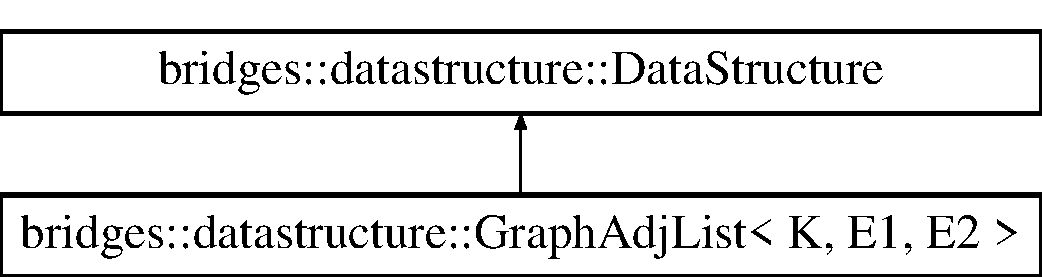
\includegraphics[height=2.000000cm]{classbridges_1_1datastructure_1_1_graph_adj_list}
\end{center}
\end{figure}


\subsection{Detailed Description}
\subsubsection*{template$<$typename K, typename E1 = K, typename E2 = E1$>$\newline
class bridges\+::datastructure\+::\+Graph\+Adj\+List$<$ K, E1, E2 $>$}

This class provides methods to represent adjacency list based graphs. 

The \hyperlink{classbridges_1_1datastructure_1_1_graph_adj_list}{Graph\+Adj\+List} class can be used to represent adjacency list based graphs in B\+R\+I\+D\+G\+ES; it takes 3 generic parameters\+: (1) K, which is an orderable key value used in accessing vertices (in constant time) using an S\+TL map. This permits data sets that need to be accessed by keys that are strings, (2) E1, for maintaining vertex specific data, and (3) E2, for maintaining edge specific data. The class is a wrapper around the C++ unordered map class and, thus, derives all its operations from it. B\+R\+I\+D\+G\+ES provides methods to visualize the graph and its contents.

The vertices of the graph are held in a C++ hashmap, for near constant time access; this enables us to use strings or integer ids for vertices. The adjacency lists are linked lists of S\+Lelemnt type, The \hyperlink{classbridges_1_1datastructure_1_1_s_lelement}{S\+Lelement} contains edge information (stored in its data as a generic). Each edge, of type \hyperlink{classbridges_1_1datastructure_1_1_edge}{Edge}, contains the source, destination vertices and link attributes (color, opacity, thickness)

Convenience method \hyperlink{classbridges_1_1datastructure_1_1_graph_adj_list_a3bde76e49be4330da895103475f8430b}{add\+Vertex()} is provided to add vertices to the graph, and \hyperlink{classbridges_1_1datastructure_1_1_graph_adj_list_a6573cc104657315196404bcef481d890}{add\+Edge()} is provided to add edges. Edges are retrieved by using the map and the adjcency list, given the vertex ids of the edge. Vertices can be styled directly from the vertex element returned by \hyperlink{classbridges_1_1datastructure_1_1_graph_adj_list_ada58af550495cee2fe454c0be0f8504e}{get\+Vertex()}, and edges are styled from a \hyperlink{classbridges_1_1datastructure_1_1_link_visualizer}{Link\+Visualizer} one can access through \hyperlink{classbridges_1_1datastructure_1_1_graph_adj_list_ae36ba10fae403339df0c36707ed13536}{get\+Link\+Visualizer()}. Here is a simple example\+: 
\begin{DoxyCode}
GraphAdjList<string, Integer, Double> graph = \textcolor{keyword}{new} GraphAdjList<string, int, double> ();
  graph.addVertex(\textcolor{stringliteral}{"a"});
  graph.addVertex(\textcolor{stringliteral}{"b"});
  graph.addEdge(\textcolor{stringliteral}{"a"}, \textcolor{stringliteral}{"b"});
  graph.getVertex(\textcolor{stringliteral}{"a"}).setShape(\textcolor{stringliteral}{"square"});
  graph.getLinkVisualizer(\textcolor{stringliteral}{"a"}, \textcolor{stringliteral}{"b"}).setColor(\textcolor{stringliteral}{"yellow"});
\end{DoxyCode}


Adjacency lists are singly linked lists using the B\+R\+I\+D\+G\+ES \hyperlink{classbridges_1_1datastructure_1_1_s_lelement}{S\+Lelement}. Iterators are provided for easy traversal of the adjacency lists. For instance,


\begin{DoxyCode}
GraphAdjList<string, int, double> graph = something();
\textcolor{keywordflow}{for} (Edge<string, double> e : graph.outgoingEdgeSetOf(\textcolor{stringliteral}{"a"}))
  System.out.println(\textcolor{stringliteral}{"a -> "}+\hyperlink{namespacebridges_1_1game_ab9a19c7ab6e2ebac2f95180e21733487ae1671797c52e15f763380b45e841ec32}{e}.getTo());
\end{DoxyCode}


Graphs can have their nodes and links affected by visual attributes. Nodes can have color, size, opacity and shape and detailed in the \hyperlink{classbridges_1_1datastructure_1_1_element_visualizer}{Element\+Visualizer} class. Edges support attributes such as color, thickness and opacity and are detailed in the \hyperlink{classbridges_1_1datastructure_1_1_link_visualizer}{Link\+Visualizer} class. \hyperlink{classbridges_1_1datastructure_1_1_element}{Element} and link attributes are set using the \hyperlink{classbridges_1_1datastructure_1_1_graph_adj_list_a097e4678b1273c29b1ac63319b4535e5}{get\+Visualizer()} and \hyperlink{classbridges_1_1datastructure_1_1_graph_adj_list_ae36ba10fae403339df0c36707ed13536}{get\+Link\+Visualizer()} methods. For instance,


\begin{DoxyCode}
GraphAdjList<string, int, double> graph = something();
  graph.addVertex(\textcolor{stringliteral}{"baskin"});
  graph.addVertex(\textcolor{stringliteral}{"robins"});
  graph.addEdge(\textcolor{stringliteral}{"baskin"},\textcolor{stringliteral}{"robins"});
  graph.getVisualizer()->setColor(\textcolor{stringliteral}{"cyan"});
  graph.getVisualizer()->setShape(\textcolor{stringliteral}{"square"});
  graph.getLinkVisualizer(\textcolor{stringliteral}{"baskin"}, \textcolor{stringliteral}{"robins"})->setColor(\textcolor{stringliteral}{"green"});
  graph.getLinkVisualizer(\textcolor{stringliteral}{"baskin"}, \textcolor{stringliteral}{"robins"})->setOpacity(\textcolor{stringliteral}{"0.5f"});
\end{DoxyCode}



\begin{DoxyParams}{Parameters}
{\em K} & used as an index to retrieve vertices, \\
\hline
{\em E1} & data type used to store vertex specific information, \\
\hline
{\em E2} & data type used to store edge specific information\\
\hline
\end{DoxyParams}
\begin{DoxyAuthor}{Author}
Kalpathi Subramanian, Erik Saule 
\end{DoxyAuthor}
\begin{DoxyDate}{Date}
Last modified 4/22/18, 7/12/19, 12/28/20, 1/5/21
\end{DoxyDate}
There is a tutorial about Graph Adjacency List \+: \href{http://bridgesuncc.github.io/tutorials/Graph_AL.html}{\tt http\+://bridgesuncc.\+github.\+io/tutorials/\+Graph\+\_\+\+A\+L.\+html}

There are two visualization engines available for graph. The small graph visualization supports all attributes of vertices and edges but is prohibitively slow on large graphs. The large graph visualization only supports locations (actually they are mandatory) and colors, all other attributes are ignored.

B\+R\+I\+D\+G\+ES picks the rendering engine automatically. But it can be forced to pick one used force\+Large\+Vizualization() and force\+Small\+Vizualization() \subsection*{Classes}
\begin{DoxyCompactItemize}
\item 
class \hyperlink{classbridges_1_1datastructure_1_1_graph_adj_list_1_1const_vertex_element_set__listhelper}{const\+Vertex\+Element\+Set\+\_\+listhelper}
\begin{DoxyCompactList}\small\item\em This is a helper class to return sets of vertices in a way that are iterable with range for loops. Students should not have to use this directly. \end{DoxyCompactList}\item 
class \hyperlink{classbridges_1_1datastructure_1_1_graph_adj_list_1_1_key_set__helper}{Key\+Set\+\_\+helper}
\item 
class \hyperlink{classbridges_1_1datastructure_1_1_graph_adj_list_1_1_vertex_element_set__listhelper}{Vertex\+Element\+Set\+\_\+listhelper}
\begin{DoxyCompactList}\small\item\em This is a helper class to return sets of vertices in a way that are iterable with range for loops. Students should have to use this directly. \end{DoxyCompactList}\end{DoxyCompactItemize}
\subsection*{Public Member Functions}
\begin{DoxyCompactItemize}
\item 
\hyperlink{classbridges_1_1datastructure_1_1_graph_adj_list_adb181bcfe104b8df8b3218ccf1b67ea5}{Graph\+Adj\+List} ()=default
\item 
\hyperlink{classbridges_1_1datastructure_1_1_graph_adj_list_ac175167a4447f3fc9c7f3e72f2f6a0b1}{Graph\+Adj\+List} (\hyperlink{classbridges_1_1datastructure_1_1_graph_adj_list}{Graph\+Adj\+List} \&\&gr)=default
\item 
virtual \hyperlink{classbridges_1_1datastructure_1_1_graph_adj_list_a17413dc27d7e60e1aa31cafa32082d12}{$\sim$\+Graph\+Adj\+List} () override
\item 
virtual const string \hyperlink{classbridges_1_1datastructure_1_1_graph_adj_list_adf1bfde5ec7192f3ee334695059f8fa6}{get\+D\+Stype} () const override
\begin{DoxyCompactList}\small\item\em Get the string representation of this data structure type. \end{DoxyCompactList}\item 
void \hyperlink{classbridges_1_1datastructure_1_1_graph_adj_list_a3bde76e49be4330da895103475f8430b}{add\+Vertex} (const K \&k, const E1 \&e=E1())
\begin{DoxyCompactList}\small\item\em Adds a vertex to the graph. \end{DoxyCompactList}\item 
void \hyperlink{classbridges_1_1datastructure_1_1_graph_adj_list_a6573cc104657315196404bcef481d890}{add\+Edge} (const K \&src, const K \&dest, const E2 \&data=E2())
\begin{DoxyCompactList}\small\item\em Add an edge with data. \end{DoxyCompactList}\item 
bool \hyperlink{classbridges_1_1datastructure_1_1_graph_adj_list_a926702012e62a91affc14b62802724e4}{is\+Edge} (const K \&src, const K \&dest)
\begin{DoxyCompactList}\small\item\em Check if there is an edge between the given vertices. \end{DoxyCompactList}\item 
const E1 \& \hyperlink{classbridges_1_1datastructure_1_1_graph_adj_list_a3a9d3875e7f6eb0d4c3500c53957b9c1}{get\+Vertex\+Data} (const K \&src) \&
\begin{DoxyCompactList}\small\item\em Gets vertex data for a graph vertex. \end{DoxyCompactList}\item 
void \hyperlink{classbridges_1_1datastructure_1_1_graph_adj_list_ab87a30e6cbaf1d2db95dce705ebdd20f}{set\+Vertex\+Data} (const K \&vert\+ID, E1 const \&data)
\begin{DoxyCompactList}\small\item\em Loads vertex specific information for a graph vertex. \end{DoxyCompactList}\item 
E2 \& \hyperlink{classbridges_1_1datastructure_1_1_graph_adj_list_ab56ec428deb9a5bc4499f42bbd710b1a}{get\+Edge\+Data} (const K \&src, const K \&dest)
\begin{DoxyCompactList}\small\item\em Gets edge data for the edge from \char`\"{}src\char`\"{} to \char`\"{}dest\char`\"{}. \end{DoxyCompactList}\item 
E2 const  \& \hyperlink{classbridges_1_1datastructure_1_1_graph_adj_list_a5c2cdffda7c983c3141ae36acc2b698d}{get\+Edge\+Data} (const K \&src, const K \&dest) const
\begin{DoxyCompactList}\small\item\em Gets edge data for the edge from \char`\"{}src\char`\"{} to \char`\"{}dest\char`\"{} -\/ const version. \end{DoxyCompactList}\item 
void \hyperlink{classbridges_1_1datastructure_1_1_graph_adj_list_a21a7e957d60e18b540dc778b1d569372}{set\+Edge\+Data} (const K \&src, const K \&dest, E2 \&data)
\begin{DoxyCompactList}\small\item\em Loads edge specific information for the edge from \char`\"{}src\char`\"{} to \char`\"{}dest\char`\"{}. \end{DoxyCompactList}\item 
unordered\+\_\+map$<$ K, \hyperlink{classbridges_1_1datastructure_1_1_element}{Element}$<$ E1 $>$ $\ast$ $>$ $\ast$ \hyperlink{classbridges_1_1datastructure_1_1_graph_adj_list_af91334de325f4be241c3c939ea9c5a36}{get\+Vertices} ()
\begin{DoxyCompactList}\small\item\em Return the graph nodes. \end{DoxyCompactList}\item 
const unordered\+\_\+map$<$ K, \hyperlink{classbridges_1_1datastructure_1_1_element}{Element}$<$ E1 $>$ $\ast$ $>$ $\ast$ \hyperlink{classbridges_1_1datastructure_1_1_graph_adj_list_a77b21cfdb87c4cf45ce29be6e7dd9791}{get\+Vertices} () const
\begin{DoxyCompactList}\small\item\em Return the graph nodes -\/ const version. \end{DoxyCompactList}\item 
const \hyperlink{classbridges_1_1datastructure_1_1_element}{Element}$<$ E1 $>$ $\ast$ \hyperlink{classbridges_1_1datastructure_1_1_graph_adj_list_ada58af550495cee2fe454c0be0f8504e}{get\+Vertex} (const K \&key) const
\begin{DoxyCompactList}\small\item\em Return the vertex corresponding to a key. \end{DoxyCompactList}\item 
\hyperlink{classbridges_1_1datastructure_1_1_element}{Element}$<$ E1 $>$ $\ast$ \hyperlink{classbridges_1_1datastructure_1_1_graph_adj_list_aa55482a035e233299d49874732113e6d}{get\+Vertex} (const K \&key)
\item 
\hyperlink{classbridges_1_1datastructure_1_1_edge}{Edge}$<$ K, E2 $>$ \hyperlink{classbridges_1_1datastructure_1_1_graph_adj_list_a2d8ff5a971516d05ff07bb1c3b73e405}{get\+Edge} (const K \&src, const K \&dest)
\begin{DoxyCompactList}\small\item\em Get the edge between src and dest vertices. \end{DoxyCompactList}\item 
const unordered\+\_\+map$<$ K, \hyperlink{classbridges_1_1datastructure_1_1_s_lelement}{S\+Lelement}$<$ \hyperlink{classbridges_1_1datastructure_1_1_edge}{Edge}$<$ K, E2 $>$ $>$ $\ast$ $>$ \& \hyperlink{classbridges_1_1datastructure_1_1_graph_adj_list_a23dad50371f073dd9a2f48e83720e86c}{get\+Adjacency\+List} () const
\begin{DoxyCompactList}\small\item\em Return the adjacency list. \end{DoxyCompactList}\item 
\hyperlink{classbridges_1_1datastructure_1_1_s_lelement}{S\+Lelement}$<$ \hyperlink{classbridges_1_1datastructure_1_1_edge}{Edge}$<$ K, E2 $>$ $>$ $\ast$ \hyperlink{classbridges_1_1datastructure_1_1_graph_adj_list_aa3df7d161ed7847a188b5818f78818d8}{get\+Adjacency\+List} (const K \&k)
\begin{DoxyCompactList}\small\item\em Returns adjacency list of a vertex with name k. \end{DoxyCompactList}\item 
const \hyperlink{classbridges_1_1datastructure_1_1_s_lelement}{S\+Lelement}$<$ \hyperlink{classbridges_1_1datastructure_1_1_edge}{Edge}$<$ K, E2 $>$ $>$ $\ast$ \hyperlink{classbridges_1_1datastructure_1_1_graph_adj_list_a1f8ea98a84017aa4bf6058475c0b3ed0}{get\+Adjacency\+List} (const K \&k) const
\item 
\hyperlink{classbridges_1_1datastructure_1_1_element_visualizer}{Element\+Visualizer} $\ast$ \hyperlink{classbridges_1_1datastructure_1_1_graph_adj_list_a097e4678b1273c29b1ac63319b4535e5}{get\+Visualizer} (const K \&k)
\begin{DoxyCompactList}\small\item\em Returns the visualizer corresponding to a graph vertex. convenient method to set attributes of the graph vertex. \end{DoxyCompactList}\item 
\hyperlink{classbridges_1_1datastructure_1_1_link_visualizer}{Link\+Visualizer} $\ast$ \hyperlink{classbridges_1_1datastructure_1_1_graph_adj_list_ae36ba10fae403339df0c36707ed13536}{get\+Link\+Visualizer} (const K \&k1, const K \&k2)
\begin{DoxyCompactList}\small\item\em Returns the link visualizer corresponding to an edge. Returns the link visualizer corresponding to two graph nodes with an existing link; error returned if no link exists. \end{DoxyCompactList}\item 
void \hyperlink{classbridges_1_1datastructure_1_1_graph_adj_list_a6860a0a153fd126ebe8b1bc40d2753a7}{force\+Large\+Visualization} (bool f)
\begin{DoxyCompactList}\small\item\em Force the rendering engine to use large graph visualization. \end{DoxyCompactList}\item 
void \hyperlink{classbridges_1_1datastructure_1_1_graph_adj_list_a9706e3df7d30320b7e7773a6423e4ff7}{force\+Small\+Visualization} (bool f)
\begin{DoxyCompactList}\small\item\em Force the rendering engine to use small graph visualization. \end{DoxyCompactList}\item 
\hyperlink{classbridges_1_1datastructure_1_1_graph_adj_list_1_1_key_set__helper}{Key\+Set\+\_\+helper} \hyperlink{classbridges_1_1datastructure_1_1_graph_adj_list_a0562e8d82499f26ad656a1dfb5f8908e}{key\+Set} () const
\item 
\hyperlink{classbridges_1_1datastructure_1_1_s_lelement}{S\+Lelement}$<$ \hyperlink{classbridges_1_1datastructure_1_1_edge}{Edge}$<$ K, E2 $>$ $>$\+::S\+Lelement\+\_\+listhelper \hyperlink{classbridges_1_1datastructure_1_1_graph_adj_list_ac066da800ab88dc2e55a89650e08bb78}{outgoing\+Edge\+Set\+Of} (K const \&k)
\begin{DoxyCompactList}\small\item\em This method is useful for iterating through a set of outgoing edges from a vertex. \end{DoxyCompactList}\item 
\hyperlink{classbridges_1_1datastructure_1_1_s_lelement}{S\+Lelement}$<$ \hyperlink{classbridges_1_1datastructure_1_1_edge}{Edge}$<$ K, E2 $>$ $>$\+::S\+Lelement\+\_\+constlisthelper \hyperlink{classbridges_1_1datastructure_1_1_graph_adj_list_ab0677da029442194925f8167cc2b8638}{outgoing\+Edge\+Set\+Of} (K const \&k) const
\begin{DoxyCompactList}\small\item\em This method is useful for iterating through a set of outgoing edges from a vertex -\/ const version. \end{DoxyCompactList}\item 
\hyperlink{classbridges_1_1datastructure_1_1_graph_adj_list_1_1_vertex_element_set__listhelper}{Vertex\+Element\+Set\+\_\+listhelper} \hyperlink{classbridges_1_1datastructure_1_1_graph_adj_list_a9dcf0bb4a68f3b02281c84e9bb69d6b3}{vertex\+Set} ()
\item 
\hyperlink{classbridges_1_1datastructure_1_1_graph_adj_list_1_1const_vertex_element_set__listhelper}{const\+Vertex\+Element\+Set\+\_\+listhelper} \hyperlink{classbridges_1_1datastructure_1_1_graph_adj_list_a5ef96f5df21b2f9743b7bb79c10cf090}{vertex\+Set} () const
\end{DoxyCompactItemize}


\subsection{Constructor \& Destructor Documentation}
\mbox{\Hypertarget{classbridges_1_1datastructure_1_1_graph_adj_list_adb181bcfe104b8df8b3218ccf1b67ea5}\label{classbridges_1_1datastructure_1_1_graph_adj_list_adb181bcfe104b8df8b3218ccf1b67ea5}} 
\index{bridges\+::datastructure\+::\+Graph\+Adj\+List@{bridges\+::datastructure\+::\+Graph\+Adj\+List}!Graph\+Adj\+List@{Graph\+Adj\+List}}
\index{Graph\+Adj\+List@{Graph\+Adj\+List}!bridges\+::datastructure\+::\+Graph\+Adj\+List@{bridges\+::datastructure\+::\+Graph\+Adj\+List}}
\subsubsection{\texorpdfstring{Graph\+Adj\+List()}{GraphAdjList()}\hspace{0.1cm}{\footnotesize\ttfamily [1/2]}}
{\footnotesize\ttfamily template$<$typename K, typename E1 = K, typename E2 = E1$>$ \\
\hyperlink{classbridges_1_1datastructure_1_1_graph_adj_list}{bridges\+::datastructure\+::\+Graph\+Adj\+List}$<$ K, E1, E2 $>$\+::\hyperlink{classbridges_1_1datastructure_1_1_graph_adj_list}{Graph\+Adj\+List} (\begin{DoxyParamCaption}{ }\end{DoxyParamCaption})\hspace{0.3cm}{\ttfamily [default]}}

\mbox{\Hypertarget{classbridges_1_1datastructure_1_1_graph_adj_list_ac175167a4447f3fc9c7f3e72f2f6a0b1}\label{classbridges_1_1datastructure_1_1_graph_adj_list_ac175167a4447f3fc9c7f3e72f2f6a0b1}} 
\index{bridges\+::datastructure\+::\+Graph\+Adj\+List@{bridges\+::datastructure\+::\+Graph\+Adj\+List}!Graph\+Adj\+List@{Graph\+Adj\+List}}
\index{Graph\+Adj\+List@{Graph\+Adj\+List}!bridges\+::datastructure\+::\+Graph\+Adj\+List@{bridges\+::datastructure\+::\+Graph\+Adj\+List}}
\subsubsection{\texorpdfstring{Graph\+Adj\+List()}{GraphAdjList()}\hspace{0.1cm}{\footnotesize\ttfamily [2/2]}}
{\footnotesize\ttfamily template$<$typename K, typename E1 = K, typename E2 = E1$>$ \\
\hyperlink{classbridges_1_1datastructure_1_1_graph_adj_list}{bridges\+::datastructure\+::\+Graph\+Adj\+List}$<$ K, E1, E2 $>$\+::\hyperlink{classbridges_1_1datastructure_1_1_graph_adj_list}{Graph\+Adj\+List} (\begin{DoxyParamCaption}\item[{\hyperlink{classbridges_1_1datastructure_1_1_graph_adj_list}{Graph\+Adj\+List}$<$ K, E1, E2 $>$ \&\&}]{gr }\end{DoxyParamCaption})\hspace{0.3cm}{\ttfamily [default]}}

\mbox{\Hypertarget{classbridges_1_1datastructure_1_1_graph_adj_list_a17413dc27d7e60e1aa31cafa32082d12}\label{classbridges_1_1datastructure_1_1_graph_adj_list_a17413dc27d7e60e1aa31cafa32082d12}} 
\index{bridges\+::datastructure\+::\+Graph\+Adj\+List@{bridges\+::datastructure\+::\+Graph\+Adj\+List}!````~Graph\+Adj\+List@{$\sim$\+Graph\+Adj\+List}}
\index{````~Graph\+Adj\+List@{$\sim$\+Graph\+Adj\+List}!bridges\+::datastructure\+::\+Graph\+Adj\+List@{bridges\+::datastructure\+::\+Graph\+Adj\+List}}
\subsubsection{\texorpdfstring{$\sim$\+Graph\+Adj\+List()}{~GraphAdjList()}}
{\footnotesize\ttfamily template$<$typename K, typename E1 = K, typename E2 = E1$>$ \\
virtual \hyperlink{classbridges_1_1datastructure_1_1_graph_adj_list}{bridges\+::datastructure\+::\+Graph\+Adj\+List}$<$ K, E1, E2 $>$\+::$\sim$\hyperlink{classbridges_1_1datastructure_1_1_graph_adj_list}{Graph\+Adj\+List} (\begin{DoxyParamCaption}{ }\end{DoxyParamCaption})\hspace{0.3cm}{\ttfamily [inline]}, {\ttfamily [override]}, {\ttfamily [virtual]}}



\subsection{Member Function Documentation}
\mbox{\Hypertarget{classbridges_1_1datastructure_1_1_graph_adj_list_a6573cc104657315196404bcef481d890}\label{classbridges_1_1datastructure_1_1_graph_adj_list_a6573cc104657315196404bcef481d890}} 
\index{bridges\+::datastructure\+::\+Graph\+Adj\+List@{bridges\+::datastructure\+::\+Graph\+Adj\+List}!add\+Edge@{add\+Edge}}
\index{add\+Edge@{add\+Edge}!bridges\+::datastructure\+::\+Graph\+Adj\+List@{bridges\+::datastructure\+::\+Graph\+Adj\+List}}
\subsubsection{\texorpdfstring{add\+Edge()}{addEdge()}}
{\footnotesize\ttfamily template$<$typename K, typename E1 = K, typename E2 = E1$>$ \\
void \hyperlink{classbridges_1_1datastructure_1_1_graph_adj_list}{bridges\+::datastructure\+::\+Graph\+Adj\+List}$<$ K, E1, E2 $>$\+::add\+Edge (\begin{DoxyParamCaption}\item[{const K \&}]{src,  }\item[{const K \&}]{dest,  }\item[{const E2 \&}]{data = {\ttfamily E2()} }\end{DoxyParamCaption})\hspace{0.3cm}{\ttfamily [inline]}}



Add an edge with data. 

Note that this function adds the edge regardless of the contents of the adjacency list; its the user\textquotesingle{}s responsibility to ensure there are no duplicates and ensure consistency.


\begin{DoxyParams}{Parameters}
{\em src} & The key of the source Vertex \\
\hline
{\em dest} & The key of the destination Vertex \\
\hline
{\em data} & The edge data \\
\hline
\end{DoxyParams}

\begin{DoxyExceptions}{Exceptions}
{\em out\+\_\+of\+\_\+range} & If \char`\"{}src\char`\"{} or \char`\"{}dest\char`\"{} is non-\/existent within this graph \\
\hline
{\em bad\+\_\+alloc} & If allocation of a graph adjacency list item failed \\
\hline
\end{DoxyExceptions}
\mbox{\Hypertarget{classbridges_1_1datastructure_1_1_graph_adj_list_a3bde76e49be4330da895103475f8430b}\label{classbridges_1_1datastructure_1_1_graph_adj_list_a3bde76e49be4330da895103475f8430b}} 
\index{bridges\+::datastructure\+::\+Graph\+Adj\+List@{bridges\+::datastructure\+::\+Graph\+Adj\+List}!add\+Vertex@{add\+Vertex}}
\index{add\+Vertex@{add\+Vertex}!bridges\+::datastructure\+::\+Graph\+Adj\+List@{bridges\+::datastructure\+::\+Graph\+Adj\+List}}
\subsubsection{\texorpdfstring{add\+Vertex()}{addVertex()}}
{\footnotesize\ttfamily template$<$typename K, typename E1 = K, typename E2 = E1$>$ \\
void \hyperlink{classbridges_1_1datastructure_1_1_graph_adj_list}{bridges\+::datastructure\+::\+Graph\+Adj\+List}$<$ K, E1, E2 $>$\+::add\+Vertex (\begin{DoxyParamCaption}\item[{const K \&}]{k,  }\item[{const E1 \&}]{e = {\ttfamily E1()} }\end{DoxyParamCaption})\hspace{0.3cm}{\ttfamily [inline]}}



Adds a vertex to the graph. 

Adds a vertex of key \char`\"{}k\char`\"{} and value \char`\"{}e\char`\"{} to the graph, and initializes its adjacency list; If this key already exists then this will not create a new vertex.


\begin{DoxyParams}{Parameters}
{\em k} & The vertex key \\
\hline
{\em e} & The vertex data \\
\hline
\end{DoxyParams}
\mbox{\Hypertarget{classbridges_1_1datastructure_1_1_graph_adj_list_a6860a0a153fd126ebe8b1bc40d2753a7}\label{classbridges_1_1datastructure_1_1_graph_adj_list_a6860a0a153fd126ebe8b1bc40d2753a7}} 
\index{bridges\+::datastructure\+::\+Graph\+Adj\+List@{bridges\+::datastructure\+::\+Graph\+Adj\+List}!force\+Large\+Visualization@{force\+Large\+Visualization}}
\index{force\+Large\+Visualization@{force\+Large\+Visualization}!bridges\+::datastructure\+::\+Graph\+Adj\+List@{bridges\+::datastructure\+::\+Graph\+Adj\+List}}
\subsubsection{\texorpdfstring{force\+Large\+Visualization()}{forceLargeVisualization()}}
{\footnotesize\ttfamily template$<$typename K, typename E1 = K, typename E2 = E1$>$ \\
void \hyperlink{classbridges_1_1datastructure_1_1_graph_adj_list}{bridges\+::datastructure\+::\+Graph\+Adj\+List}$<$ K, E1, E2 $>$\+::force\+Large\+Visualization (\begin{DoxyParamCaption}\item[{bool}]{f }\end{DoxyParamCaption})\hspace{0.3cm}{\ttfamily [inline]}}



Force the rendering engine to use large graph visualization. 

This forces the rendering to a more bandwidth efficient at the cost of having less features. The large graph visualization only renders vertices that have specified locations. The only usable attribute for vertices and edges are colors.


\begin{DoxyParams}{Parameters}
{\em f} & set to true to force the visualization engine to use large graphs visualization. Setting to false does not prevent large visualization to be used, just does not force it. \\
\hline
\end{DoxyParams}
\mbox{\Hypertarget{classbridges_1_1datastructure_1_1_graph_adj_list_a9706e3df7d30320b7e7773a6423e4ff7}\label{classbridges_1_1datastructure_1_1_graph_adj_list_a9706e3df7d30320b7e7773a6423e4ff7}} 
\index{bridges\+::datastructure\+::\+Graph\+Adj\+List@{bridges\+::datastructure\+::\+Graph\+Adj\+List}!force\+Small\+Visualization@{force\+Small\+Visualization}}
\index{force\+Small\+Visualization@{force\+Small\+Visualization}!bridges\+::datastructure\+::\+Graph\+Adj\+List@{bridges\+::datastructure\+::\+Graph\+Adj\+List}}
\subsubsection{\texorpdfstring{force\+Small\+Visualization()}{forceSmallVisualization()}}
{\footnotesize\ttfamily template$<$typename K, typename E1 = K, typename E2 = E1$>$ \\
void \hyperlink{classbridges_1_1datastructure_1_1_graph_adj_list}{bridges\+::datastructure\+::\+Graph\+Adj\+List}$<$ K, E1, E2 $>$\+::force\+Small\+Visualization (\begin{DoxyParamCaption}\item[{bool}]{f }\end{DoxyParamCaption})\hspace{0.3cm}{\ttfamily [inline]}}



Force the rendering engine to use small graph visualization. 

The small visualization uses more bandwidth, have more features, and support a force directed layout for vertices which do not have a specified location.


\begin{DoxyParams}{Parameters}
{\em f} & set to true to force the visualization engine to use small graphs visualization. Setting to false does not prevent small visualization to be used, just does not force it. \\
\hline
\end{DoxyParams}
\mbox{\Hypertarget{classbridges_1_1datastructure_1_1_graph_adj_list_a23dad50371f073dd9a2f48e83720e86c}\label{classbridges_1_1datastructure_1_1_graph_adj_list_a23dad50371f073dd9a2f48e83720e86c}} 
\index{bridges\+::datastructure\+::\+Graph\+Adj\+List@{bridges\+::datastructure\+::\+Graph\+Adj\+List}!get\+Adjacency\+List@{get\+Adjacency\+List}}
\index{get\+Adjacency\+List@{get\+Adjacency\+List}!bridges\+::datastructure\+::\+Graph\+Adj\+List@{bridges\+::datastructure\+::\+Graph\+Adj\+List}}
\subsubsection{\texorpdfstring{get\+Adjacency\+List()}{getAdjacencyList()}\hspace{0.1cm}{\footnotesize\ttfamily [1/3]}}
{\footnotesize\ttfamily template$<$typename K, typename E1 = K, typename E2 = E1$>$ \\
const unordered\+\_\+map$<$K, \hyperlink{classbridges_1_1datastructure_1_1_s_lelement}{S\+Lelement}$<$\hyperlink{classbridges_1_1datastructure_1_1_edge}{Edge}$<$K, E2$>$ $>$$\ast$$>$\& \hyperlink{classbridges_1_1datastructure_1_1_graph_adj_list}{bridges\+::datastructure\+::\+Graph\+Adj\+List}$<$ K, E1, E2 $>$\+::get\+Adjacency\+List (\begin{DoxyParamCaption}{ }\end{DoxyParamCaption}) const\hspace{0.3cm}{\ttfamily [inline]}}



Return the adjacency list. 

\begin{DoxyReturn}{Returns}
The adjacency list of the graph 
\end{DoxyReturn}
\mbox{\Hypertarget{classbridges_1_1datastructure_1_1_graph_adj_list_aa3df7d161ed7847a188b5818f78818d8}\label{classbridges_1_1datastructure_1_1_graph_adj_list_aa3df7d161ed7847a188b5818f78818d8}} 
\index{bridges\+::datastructure\+::\+Graph\+Adj\+List@{bridges\+::datastructure\+::\+Graph\+Adj\+List}!get\+Adjacency\+List@{get\+Adjacency\+List}}
\index{get\+Adjacency\+List@{get\+Adjacency\+List}!bridges\+::datastructure\+::\+Graph\+Adj\+List@{bridges\+::datastructure\+::\+Graph\+Adj\+List}}
\subsubsection{\texorpdfstring{get\+Adjacency\+List()}{getAdjacencyList()}\hspace{0.1cm}{\footnotesize\ttfamily [2/3]}}
{\footnotesize\ttfamily template$<$typename K, typename E1 = K, typename E2 = E1$>$ \\
\hyperlink{classbridges_1_1datastructure_1_1_s_lelement}{S\+Lelement}$<$\hyperlink{classbridges_1_1datastructure_1_1_edge}{Edge}$<$K, E2$>$ $>$$\ast$ \hyperlink{classbridges_1_1datastructure_1_1_graph_adj_list}{bridges\+::datastructure\+::\+Graph\+Adj\+List}$<$ K, E1, E2 $>$\+::get\+Adjacency\+List (\begin{DoxyParamCaption}\item[{const K \&}]{k }\end{DoxyParamCaption})\hspace{0.3cm}{\ttfamily [inline]}}



Returns adjacency list of a vertex with name k. 


\begin{DoxyParams}{Parameters}
{\em k} & The key of the source vertex \\
\hline
\end{DoxyParams}

\begin{DoxyExceptions}{Exceptions}
{\em out\+\_\+of\+\_\+range} & If key is non-\/existent within this graph\\
\hline
\end{DoxyExceptions}
\begin{DoxyReturn}{Returns}
The adjacency list of key \char`\"{}k\char`\"{} 
\end{DoxyReturn}
\mbox{\Hypertarget{classbridges_1_1datastructure_1_1_graph_adj_list_a1f8ea98a84017aa4bf6058475c0b3ed0}\label{classbridges_1_1datastructure_1_1_graph_adj_list_a1f8ea98a84017aa4bf6058475c0b3ed0}} 
\index{bridges\+::datastructure\+::\+Graph\+Adj\+List@{bridges\+::datastructure\+::\+Graph\+Adj\+List}!get\+Adjacency\+List@{get\+Adjacency\+List}}
\index{get\+Adjacency\+List@{get\+Adjacency\+List}!bridges\+::datastructure\+::\+Graph\+Adj\+List@{bridges\+::datastructure\+::\+Graph\+Adj\+List}}
\subsubsection{\texorpdfstring{get\+Adjacency\+List()}{getAdjacencyList()}\hspace{0.1cm}{\footnotesize\ttfamily [3/3]}}
{\footnotesize\ttfamily template$<$typename K, typename E1 = K, typename E2 = E1$>$ \\
const \hyperlink{classbridges_1_1datastructure_1_1_s_lelement}{S\+Lelement}$<$\hyperlink{classbridges_1_1datastructure_1_1_edge}{Edge}$<$K, E2$>$ $>$$\ast$ \hyperlink{classbridges_1_1datastructure_1_1_graph_adj_list}{bridges\+::datastructure\+::\+Graph\+Adj\+List}$<$ K, E1, E2 $>$\+::get\+Adjacency\+List (\begin{DoxyParamCaption}\item[{const K \&}]{k }\end{DoxyParamCaption}) const\hspace{0.3cm}{\ttfamily [inline]}}

Returns adjacency list of a vertex with name k -\/ const version


\begin{DoxyParams}{Parameters}
{\em k} & The key of the source vertex \\
\hline
\end{DoxyParams}

\begin{DoxyExceptions}{Exceptions}
{\em out\+\_\+of\+\_\+range} & If key is non-\/existent within this graph\\
\hline
\end{DoxyExceptions}
\begin{DoxyReturn}{Returns}
The adjacency list of key \char`\"{}k\char`\"{} 
\end{DoxyReturn}
\mbox{\Hypertarget{classbridges_1_1datastructure_1_1_graph_adj_list_adf1bfde5ec7192f3ee334695059f8fa6}\label{classbridges_1_1datastructure_1_1_graph_adj_list_adf1bfde5ec7192f3ee334695059f8fa6}} 
\index{bridges\+::datastructure\+::\+Graph\+Adj\+List@{bridges\+::datastructure\+::\+Graph\+Adj\+List}!get\+D\+Stype@{get\+D\+Stype}}
\index{get\+D\+Stype@{get\+D\+Stype}!bridges\+::datastructure\+::\+Graph\+Adj\+List@{bridges\+::datastructure\+::\+Graph\+Adj\+List}}
\subsubsection{\texorpdfstring{get\+D\+Stype()}{getDStype()}}
{\footnotesize\ttfamily template$<$typename K, typename E1 = K, typename E2 = E1$>$ \\
virtual const string \hyperlink{classbridges_1_1datastructure_1_1_graph_adj_list}{bridges\+::datastructure\+::\+Graph\+Adj\+List}$<$ K, E1, E2 $>$\+::get\+D\+Stype (\begin{DoxyParamCaption}{ }\end{DoxyParamCaption}) const\hspace{0.3cm}{\ttfamily [inline]}, {\ttfamily [override]}, {\ttfamily [virtual]}}



Get the string representation of this data structure type. 

\begin{DoxyReturn}{Returns}
The string representation of this data structure type 
\end{DoxyReturn}


Implements \hyperlink{classbridges_1_1datastructure_1_1_data_structure_a4ff66cb34409f11fe9fc647f6d8a22ce}{bridges\+::datastructure\+::\+Data\+Structure}.

\mbox{\Hypertarget{classbridges_1_1datastructure_1_1_graph_adj_list_a2d8ff5a971516d05ff07bb1c3b73e405}\label{classbridges_1_1datastructure_1_1_graph_adj_list_a2d8ff5a971516d05ff07bb1c3b73e405}} 
\index{bridges\+::datastructure\+::\+Graph\+Adj\+List@{bridges\+::datastructure\+::\+Graph\+Adj\+List}!get\+Edge@{get\+Edge}}
\index{get\+Edge@{get\+Edge}!bridges\+::datastructure\+::\+Graph\+Adj\+List@{bridges\+::datastructure\+::\+Graph\+Adj\+List}}
\subsubsection{\texorpdfstring{get\+Edge()}{getEdge()}}
{\footnotesize\ttfamily template$<$typename K, typename E1 = K, typename E2 = E1$>$ \\
\hyperlink{classbridges_1_1datastructure_1_1_edge}{Edge}$<$K, E2$>$ \hyperlink{classbridges_1_1datastructure_1_1_graph_adj_list}{bridges\+::datastructure\+::\+Graph\+Adj\+List}$<$ K, E1, E2 $>$\+::get\+Edge (\begin{DoxyParamCaption}\item[{const K \&}]{src,  }\item[{const K \&}]{dest }\end{DoxyParamCaption})\hspace{0.3cm}{\ttfamily [inline]}}



Get the edge between src and dest vertices. 


\begin{DoxyParams}{Parameters}
{\em src} & source vertex of edge \\
\hline
{\em dest} & destination vertex of edge \\
\hline
\end{DoxyParams}
\begin{DoxyReturn}{Returns}
edge between the vertices 
\end{DoxyReturn}
\mbox{\Hypertarget{classbridges_1_1datastructure_1_1_graph_adj_list_ab56ec428deb9a5bc4499f42bbd710b1a}\label{classbridges_1_1datastructure_1_1_graph_adj_list_ab56ec428deb9a5bc4499f42bbd710b1a}} 
\index{bridges\+::datastructure\+::\+Graph\+Adj\+List@{bridges\+::datastructure\+::\+Graph\+Adj\+List}!get\+Edge\+Data@{get\+Edge\+Data}}
\index{get\+Edge\+Data@{get\+Edge\+Data}!bridges\+::datastructure\+::\+Graph\+Adj\+List@{bridges\+::datastructure\+::\+Graph\+Adj\+List}}
\subsubsection{\texorpdfstring{get\+Edge\+Data()}{getEdgeData()}\hspace{0.1cm}{\footnotesize\ttfamily [1/2]}}
{\footnotesize\ttfamily template$<$typename K, typename E1 = K, typename E2 = E1$>$ \\
E2\& \hyperlink{classbridges_1_1datastructure_1_1_graph_adj_list}{bridges\+::datastructure\+::\+Graph\+Adj\+List}$<$ K, E1, E2 $>$\+::get\+Edge\+Data (\begin{DoxyParamCaption}\item[{const K \&}]{src,  }\item[{const K \&}]{dest }\end{DoxyParamCaption})\hspace{0.3cm}{\ttfamily [inline]}}



Gets edge data for the edge from \char`\"{}src\char`\"{} to \char`\"{}dest\char`\"{}. 


\begin{DoxyParams}{Parameters}
{\em src} & The key of the source Vertex \\
\hline
{\em dest} & The key of the destination Vertex\\
\hline
\end{DoxyParams}
\begin{DoxyReturn}{Returns}
edge specific data 
\end{DoxyReturn}
\mbox{\Hypertarget{classbridges_1_1datastructure_1_1_graph_adj_list_a5c2cdffda7c983c3141ae36acc2b698d}\label{classbridges_1_1datastructure_1_1_graph_adj_list_a5c2cdffda7c983c3141ae36acc2b698d}} 
\index{bridges\+::datastructure\+::\+Graph\+Adj\+List@{bridges\+::datastructure\+::\+Graph\+Adj\+List}!get\+Edge\+Data@{get\+Edge\+Data}}
\index{get\+Edge\+Data@{get\+Edge\+Data}!bridges\+::datastructure\+::\+Graph\+Adj\+List@{bridges\+::datastructure\+::\+Graph\+Adj\+List}}
\subsubsection{\texorpdfstring{get\+Edge\+Data()}{getEdgeData()}\hspace{0.1cm}{\footnotesize\ttfamily [2/2]}}
{\footnotesize\ttfamily template$<$typename K, typename E1 = K, typename E2 = E1$>$ \\
E2 const\& \hyperlink{classbridges_1_1datastructure_1_1_graph_adj_list}{bridges\+::datastructure\+::\+Graph\+Adj\+List}$<$ K, E1, E2 $>$\+::get\+Edge\+Data (\begin{DoxyParamCaption}\item[{const K \&}]{src,  }\item[{const K \&}]{dest }\end{DoxyParamCaption}) const\hspace{0.3cm}{\ttfamily [inline]}}



Gets edge data for the edge from \char`\"{}src\char`\"{} to \char`\"{}dest\char`\"{} -\/ const version. 


\begin{DoxyParams}{Parameters}
{\em src} & The key of the source Vertex \\
\hline
{\em dest} & The key of the destination Vertex\\
\hline
\end{DoxyParams}
\begin{DoxyReturn}{Returns}
edge specific data 
\end{DoxyReturn}
\mbox{\Hypertarget{classbridges_1_1datastructure_1_1_graph_adj_list_ae36ba10fae403339df0c36707ed13536}\label{classbridges_1_1datastructure_1_1_graph_adj_list_ae36ba10fae403339df0c36707ed13536}} 
\index{bridges\+::datastructure\+::\+Graph\+Adj\+List@{bridges\+::datastructure\+::\+Graph\+Adj\+List}!get\+Link\+Visualizer@{get\+Link\+Visualizer}}
\index{get\+Link\+Visualizer@{get\+Link\+Visualizer}!bridges\+::datastructure\+::\+Graph\+Adj\+List@{bridges\+::datastructure\+::\+Graph\+Adj\+List}}
\subsubsection{\texorpdfstring{get\+Link\+Visualizer()}{getLinkVisualizer()}}
{\footnotesize\ttfamily template$<$typename K, typename E1 = K, typename E2 = E1$>$ \\
\hyperlink{classbridges_1_1datastructure_1_1_link_visualizer}{Link\+Visualizer}$\ast$ \hyperlink{classbridges_1_1datastructure_1_1_graph_adj_list}{bridges\+::datastructure\+::\+Graph\+Adj\+List}$<$ K, E1, E2 $>$\+::get\+Link\+Visualizer (\begin{DoxyParamCaption}\item[{const K \&}]{k1,  }\item[{const K \&}]{k2 }\end{DoxyParamCaption})\hspace{0.3cm}{\ttfamily [inline]}}



Returns the link visualizer corresponding to an edge. Returns the link visualizer corresponding to two graph nodes with an existing link; error returned if no link exists. 


\begin{DoxyParams}{Parameters}
{\em k1} & The key of the link source vertex \\
\hline
{\em k2} & The key of the link destination vertex\\
\hline
\end{DoxyParams}
\begin{DoxyReturn}{Returns}
the visualizer that controls the attributes of this link 
\end{DoxyReturn}
\mbox{\Hypertarget{classbridges_1_1datastructure_1_1_graph_adj_list_ada58af550495cee2fe454c0be0f8504e}\label{classbridges_1_1datastructure_1_1_graph_adj_list_ada58af550495cee2fe454c0be0f8504e}} 
\index{bridges\+::datastructure\+::\+Graph\+Adj\+List@{bridges\+::datastructure\+::\+Graph\+Adj\+List}!get\+Vertex@{get\+Vertex}}
\index{get\+Vertex@{get\+Vertex}!bridges\+::datastructure\+::\+Graph\+Adj\+List@{bridges\+::datastructure\+::\+Graph\+Adj\+List}}
\subsubsection{\texorpdfstring{get\+Vertex()}{getVertex()}\hspace{0.1cm}{\footnotesize\ttfamily [1/2]}}
{\footnotesize\ttfamily template$<$typename K, typename E1 = K, typename E2 = E1$>$ \\
const \hyperlink{classbridges_1_1datastructure_1_1_element}{Element}$<$E1$>$$\ast$ \hyperlink{classbridges_1_1datastructure_1_1_graph_adj_list}{bridges\+::datastructure\+::\+Graph\+Adj\+List}$<$ K, E1, E2 $>$\+::get\+Vertex (\begin{DoxyParamCaption}\item[{const K \&}]{key }\end{DoxyParamCaption}) const\hspace{0.3cm}{\ttfamily [inline]}}



Return the vertex corresponding to a key. 

\begin{DoxyReturn}{Returns}
the requested vertex of this graph or nullptr if not found 
\end{DoxyReturn}
\mbox{\Hypertarget{classbridges_1_1datastructure_1_1_graph_adj_list_aa55482a035e233299d49874732113e6d}\label{classbridges_1_1datastructure_1_1_graph_adj_list_aa55482a035e233299d49874732113e6d}} 
\index{bridges\+::datastructure\+::\+Graph\+Adj\+List@{bridges\+::datastructure\+::\+Graph\+Adj\+List}!get\+Vertex@{get\+Vertex}}
\index{get\+Vertex@{get\+Vertex}!bridges\+::datastructure\+::\+Graph\+Adj\+List@{bridges\+::datastructure\+::\+Graph\+Adj\+List}}
\subsubsection{\texorpdfstring{get\+Vertex()}{getVertex()}\hspace{0.1cm}{\footnotesize\ttfamily [2/2]}}
{\footnotesize\ttfamily template$<$typename K, typename E1 = K, typename E2 = E1$>$ \\
\hyperlink{classbridges_1_1datastructure_1_1_element}{Element}$<$E1$>$$\ast$ \hyperlink{classbridges_1_1datastructure_1_1_graph_adj_list}{bridges\+::datastructure\+::\+Graph\+Adj\+List}$<$ K, E1, E2 $>$\+::get\+Vertex (\begin{DoxyParamCaption}\item[{const K \&}]{key }\end{DoxyParamCaption})\hspace{0.3cm}{\ttfamily [inline]}}

Return the requested vertex corresponding to a key -\/ non-\/const version \begin{DoxyReturn}{Returns}
the requested vertex of this graph or nullptr if not found 
\end{DoxyReturn}
\mbox{\Hypertarget{classbridges_1_1datastructure_1_1_graph_adj_list_a3a9d3875e7f6eb0d4c3500c53957b9c1}\label{classbridges_1_1datastructure_1_1_graph_adj_list_a3a9d3875e7f6eb0d4c3500c53957b9c1}} 
\index{bridges\+::datastructure\+::\+Graph\+Adj\+List@{bridges\+::datastructure\+::\+Graph\+Adj\+List}!get\+Vertex\+Data@{get\+Vertex\+Data}}
\index{get\+Vertex\+Data@{get\+Vertex\+Data}!bridges\+::datastructure\+::\+Graph\+Adj\+List@{bridges\+::datastructure\+::\+Graph\+Adj\+List}}
\subsubsection{\texorpdfstring{get\+Vertex\+Data()}{getVertexData()}}
{\footnotesize\ttfamily template$<$typename K, typename E1 = K, typename E2 = E1$>$ \\
const E1\& \hyperlink{classbridges_1_1datastructure_1_1_graph_adj_list}{bridges\+::datastructure\+::\+Graph\+Adj\+List}$<$ K, E1, E2 $>$\+::get\+Vertex\+Data (\begin{DoxyParamCaption}\item[{const K \&}]{src }\end{DoxyParamCaption}) \&\hspace{0.3cm}{\ttfamily [inline]}}



Gets vertex data for a graph vertex. 


\begin{DoxyParams}{Parameters}
{\em src} & The key of the source vertex\\
\hline
\end{DoxyParams}
\begin{DoxyReturn}{Returns}
E1 vertex specific data 
\end{DoxyReturn}
\mbox{\Hypertarget{classbridges_1_1datastructure_1_1_graph_adj_list_af91334de325f4be241c3c939ea9c5a36}\label{classbridges_1_1datastructure_1_1_graph_adj_list_af91334de325f4be241c3c939ea9c5a36}} 
\index{bridges\+::datastructure\+::\+Graph\+Adj\+List@{bridges\+::datastructure\+::\+Graph\+Adj\+List}!get\+Vertices@{get\+Vertices}}
\index{get\+Vertices@{get\+Vertices}!bridges\+::datastructure\+::\+Graph\+Adj\+List@{bridges\+::datastructure\+::\+Graph\+Adj\+List}}
\subsubsection{\texorpdfstring{get\+Vertices()}{getVertices()}\hspace{0.1cm}{\footnotesize\ttfamily [1/2]}}
{\footnotesize\ttfamily template$<$typename K, typename E1 = K, typename E2 = E1$>$ \\
unordered\+\_\+map$<$K, \hyperlink{classbridges_1_1datastructure_1_1_element}{Element}$<$E1$>$$\ast$$>$$\ast$ \hyperlink{classbridges_1_1datastructure_1_1_graph_adj_list}{bridges\+::datastructure\+::\+Graph\+Adj\+List}$<$ K, E1, E2 $>$\+::get\+Vertices (\begin{DoxyParamCaption}{ }\end{DoxyParamCaption})\hspace{0.3cm}{\ttfamily [inline]}}



Return the graph nodes. 

\begin{DoxyReturn}{Returns}
The vertex list of this graph 
\end{DoxyReturn}
\mbox{\Hypertarget{classbridges_1_1datastructure_1_1_graph_adj_list_a77b21cfdb87c4cf45ce29be6e7dd9791}\label{classbridges_1_1datastructure_1_1_graph_adj_list_a77b21cfdb87c4cf45ce29be6e7dd9791}} 
\index{bridges\+::datastructure\+::\+Graph\+Adj\+List@{bridges\+::datastructure\+::\+Graph\+Adj\+List}!get\+Vertices@{get\+Vertices}}
\index{get\+Vertices@{get\+Vertices}!bridges\+::datastructure\+::\+Graph\+Adj\+List@{bridges\+::datastructure\+::\+Graph\+Adj\+List}}
\subsubsection{\texorpdfstring{get\+Vertices()}{getVertices()}\hspace{0.1cm}{\footnotesize\ttfamily [2/2]}}
{\footnotesize\ttfamily template$<$typename K, typename E1 = K, typename E2 = E1$>$ \\
const unordered\+\_\+map$<$K, \hyperlink{classbridges_1_1datastructure_1_1_element}{Element}$<$E1$>$$\ast$$>$$\ast$ \hyperlink{classbridges_1_1datastructure_1_1_graph_adj_list}{bridges\+::datastructure\+::\+Graph\+Adj\+List}$<$ K, E1, E2 $>$\+::get\+Vertices (\begin{DoxyParamCaption}{ }\end{DoxyParamCaption}) const\hspace{0.3cm}{\ttfamily [inline]}}



Return the graph nodes -\/ const version. 

\begin{DoxyReturn}{Returns}
The vertex list of this graph 
\end{DoxyReturn}
\mbox{\Hypertarget{classbridges_1_1datastructure_1_1_graph_adj_list_a097e4678b1273c29b1ac63319b4535e5}\label{classbridges_1_1datastructure_1_1_graph_adj_list_a097e4678b1273c29b1ac63319b4535e5}} 
\index{bridges\+::datastructure\+::\+Graph\+Adj\+List@{bridges\+::datastructure\+::\+Graph\+Adj\+List}!get\+Visualizer@{get\+Visualizer}}
\index{get\+Visualizer@{get\+Visualizer}!bridges\+::datastructure\+::\+Graph\+Adj\+List@{bridges\+::datastructure\+::\+Graph\+Adj\+List}}
\subsubsection{\texorpdfstring{get\+Visualizer()}{getVisualizer()}}
{\footnotesize\ttfamily template$<$typename K, typename E1 = K, typename E2 = E1$>$ \\
\hyperlink{classbridges_1_1datastructure_1_1_element_visualizer}{Element\+Visualizer}$\ast$ \hyperlink{classbridges_1_1datastructure_1_1_graph_adj_list}{bridges\+::datastructure\+::\+Graph\+Adj\+List}$<$ K, E1, E2 $>$\+::get\+Visualizer (\begin{DoxyParamCaption}\item[{const K \&}]{k }\end{DoxyParamCaption})\hspace{0.3cm}{\ttfamily [inline]}}



Returns the visualizer corresponding to a graph vertex. convenient method to set attributes of the graph vertex. 


\begin{DoxyParams}{Parameters}
{\em k} & The key of the graph vertex\\
\hline
\end{DoxyParams}
\begin{DoxyReturn}{Returns}
the visualizer that controls the attributes of this node 
\end{DoxyReturn}
\mbox{\Hypertarget{classbridges_1_1datastructure_1_1_graph_adj_list_a926702012e62a91affc14b62802724e4}\label{classbridges_1_1datastructure_1_1_graph_adj_list_a926702012e62a91affc14b62802724e4}} 
\index{bridges\+::datastructure\+::\+Graph\+Adj\+List@{bridges\+::datastructure\+::\+Graph\+Adj\+List}!is\+Edge@{is\+Edge}}
\index{is\+Edge@{is\+Edge}!bridges\+::datastructure\+::\+Graph\+Adj\+List@{bridges\+::datastructure\+::\+Graph\+Adj\+List}}
\subsubsection{\texorpdfstring{is\+Edge()}{isEdge()}}
{\footnotesize\ttfamily template$<$typename K, typename E1 = K, typename E2 = E1$>$ \\
bool \hyperlink{classbridges_1_1datastructure_1_1_graph_adj_list}{bridges\+::datastructure\+::\+Graph\+Adj\+List}$<$ K, E1, E2 $>$\+::is\+Edge (\begin{DoxyParamCaption}\item[{const K \&}]{src,  }\item[{const K \&}]{dest }\end{DoxyParamCaption})\hspace{0.3cm}{\ttfamily [inline]}}



Check if there is an edge between the given vertices. 


\begin{DoxyParams}{Parameters}
{\em src} & The key of the source Vertex \\
\hline
{\em dest} & The key of the destination Vertex \\
\hline
\end{DoxyParams}
\mbox{\Hypertarget{classbridges_1_1datastructure_1_1_graph_adj_list_a0562e8d82499f26ad656a1dfb5f8908e}\label{classbridges_1_1datastructure_1_1_graph_adj_list_a0562e8d82499f26ad656a1dfb5f8908e}} 
\index{bridges\+::datastructure\+::\+Graph\+Adj\+List@{bridges\+::datastructure\+::\+Graph\+Adj\+List}!key\+Set@{key\+Set}}
\index{key\+Set@{key\+Set}!bridges\+::datastructure\+::\+Graph\+Adj\+List@{bridges\+::datastructure\+::\+Graph\+Adj\+List}}
\subsubsection{\texorpdfstring{key\+Set()}{keySet()}}
{\footnotesize\ttfamily template$<$typename K, typename E1 = K, typename E2 = E1$>$ \\
\hyperlink{classbridges_1_1datastructure_1_1_graph_adj_list_1_1_key_set__helper}{Key\+Set\+\_\+helper} \hyperlink{classbridges_1_1datastructure_1_1_graph_adj_list}{bridges\+::datastructure\+::\+Graph\+Adj\+List}$<$ K, E1, E2 $>$\+::key\+Set (\begin{DoxyParamCaption}{ }\end{DoxyParamCaption}) const\hspace{0.3cm}{\ttfamily [inline]}}

Returns a set of all keys (helper function).

Returns a set of all keys (read only) that conforms to S\+TL list interface. That means we can use range for loops on graph vertices.

\begin{DoxyReturn}{Returns}
set all keys 
\end{DoxyReturn}
\mbox{\Hypertarget{classbridges_1_1datastructure_1_1_graph_adj_list_ac066da800ab88dc2e55a89650e08bb78}\label{classbridges_1_1datastructure_1_1_graph_adj_list_ac066da800ab88dc2e55a89650e08bb78}} 
\index{bridges\+::datastructure\+::\+Graph\+Adj\+List@{bridges\+::datastructure\+::\+Graph\+Adj\+List}!outgoing\+Edge\+Set\+Of@{outgoing\+Edge\+Set\+Of}}
\index{outgoing\+Edge\+Set\+Of@{outgoing\+Edge\+Set\+Of}!bridges\+::datastructure\+::\+Graph\+Adj\+List@{bridges\+::datastructure\+::\+Graph\+Adj\+List}}
\subsubsection{\texorpdfstring{outgoing\+Edge\+Set\+Of()}{outgoingEdgeSetOf()}\hspace{0.1cm}{\footnotesize\ttfamily [1/2]}}
{\footnotesize\ttfamily template$<$typename K, typename E1 = K, typename E2 = E1$>$ \\
\hyperlink{classbridges_1_1datastructure_1_1_s_lelement}{S\+Lelement}$<$\hyperlink{classbridges_1_1datastructure_1_1_edge}{Edge}$<$K, E2$>$ $>$\+::S\+Lelement\+\_\+listhelper \hyperlink{classbridges_1_1datastructure_1_1_graph_adj_list}{bridges\+::datastructure\+::\+Graph\+Adj\+List}$<$ K, E1, E2 $>$\+::outgoing\+Edge\+Set\+Of (\begin{DoxyParamCaption}\item[{K const \&}]{k }\end{DoxyParamCaption})\hspace{0.3cm}{\ttfamily [inline]}}



This method is useful for iterating through a set of outgoing edges from a vertex. 

\mbox{\Hypertarget{classbridges_1_1datastructure_1_1_graph_adj_list_ab0677da029442194925f8167cc2b8638}\label{classbridges_1_1datastructure_1_1_graph_adj_list_ab0677da029442194925f8167cc2b8638}} 
\index{bridges\+::datastructure\+::\+Graph\+Adj\+List@{bridges\+::datastructure\+::\+Graph\+Adj\+List}!outgoing\+Edge\+Set\+Of@{outgoing\+Edge\+Set\+Of}}
\index{outgoing\+Edge\+Set\+Of@{outgoing\+Edge\+Set\+Of}!bridges\+::datastructure\+::\+Graph\+Adj\+List@{bridges\+::datastructure\+::\+Graph\+Adj\+List}}
\subsubsection{\texorpdfstring{outgoing\+Edge\+Set\+Of()}{outgoingEdgeSetOf()}\hspace{0.1cm}{\footnotesize\ttfamily [2/2]}}
{\footnotesize\ttfamily template$<$typename K, typename E1 = K, typename E2 = E1$>$ \\
\hyperlink{classbridges_1_1datastructure_1_1_s_lelement}{S\+Lelement}$<$\hyperlink{classbridges_1_1datastructure_1_1_edge}{Edge}$<$K, E2$>$ $>$\+::S\+Lelement\+\_\+constlisthelper \hyperlink{classbridges_1_1datastructure_1_1_graph_adj_list}{bridges\+::datastructure\+::\+Graph\+Adj\+List}$<$ K, E1, E2 $>$\+::outgoing\+Edge\+Set\+Of (\begin{DoxyParamCaption}\item[{K const \&}]{k }\end{DoxyParamCaption}) const\hspace{0.3cm}{\ttfamily [inline]}}



This method is useful for iterating through a set of outgoing edges from a vertex -\/ const version. 

\mbox{\Hypertarget{classbridges_1_1datastructure_1_1_graph_adj_list_a21a7e957d60e18b540dc778b1d569372}\label{classbridges_1_1datastructure_1_1_graph_adj_list_a21a7e957d60e18b540dc778b1d569372}} 
\index{bridges\+::datastructure\+::\+Graph\+Adj\+List@{bridges\+::datastructure\+::\+Graph\+Adj\+List}!set\+Edge\+Data@{set\+Edge\+Data}}
\index{set\+Edge\+Data@{set\+Edge\+Data}!bridges\+::datastructure\+::\+Graph\+Adj\+List@{bridges\+::datastructure\+::\+Graph\+Adj\+List}}
\subsubsection{\texorpdfstring{set\+Edge\+Data()}{setEdgeData()}}
{\footnotesize\ttfamily template$<$typename K, typename E1 = K, typename E2 = E1$>$ \\
void \hyperlink{classbridges_1_1datastructure_1_1_graph_adj_list}{bridges\+::datastructure\+::\+Graph\+Adj\+List}$<$ K, E1, E2 $>$\+::set\+Edge\+Data (\begin{DoxyParamCaption}\item[{const K \&}]{src,  }\item[{const K \&}]{dest,  }\item[{E2 \&}]{data }\end{DoxyParamCaption})\hspace{0.3cm}{\ttfamily [inline]}}



Loads edge specific information for the edge from \char`\"{}src\char`\"{} to \char`\"{}dest\char`\"{}. 


\begin{DoxyParams}{Parameters}
{\em src} & The key of the source Vertex \\
\hline
{\em dest} & The key of the destination Vertex \\
\hline
{\em data} & edge data \\
\hline
\end{DoxyParams}
\mbox{\Hypertarget{classbridges_1_1datastructure_1_1_graph_adj_list_ab87a30e6cbaf1d2db95dce705ebdd20f}\label{classbridges_1_1datastructure_1_1_graph_adj_list_ab87a30e6cbaf1d2db95dce705ebdd20f}} 
\index{bridges\+::datastructure\+::\+Graph\+Adj\+List@{bridges\+::datastructure\+::\+Graph\+Adj\+List}!set\+Vertex\+Data@{set\+Vertex\+Data}}
\index{set\+Vertex\+Data@{set\+Vertex\+Data}!bridges\+::datastructure\+::\+Graph\+Adj\+List@{bridges\+::datastructure\+::\+Graph\+Adj\+List}}
\subsubsection{\texorpdfstring{set\+Vertex\+Data()}{setVertexData()}}
{\footnotesize\ttfamily template$<$typename K, typename E1 = K, typename E2 = E1$>$ \\
void \hyperlink{classbridges_1_1datastructure_1_1_graph_adj_list}{bridges\+::datastructure\+::\+Graph\+Adj\+List}$<$ K, E1, E2 $>$\+::set\+Vertex\+Data (\begin{DoxyParamCaption}\item[{const K \&}]{vert\+ID,  }\item[{E1 const \&}]{data }\end{DoxyParamCaption})\hspace{0.3cm}{\ttfamily [inline]}}



Loads vertex specific information for a graph vertex. 


\begin{DoxyParams}{Parameters}
{\em vert\+ID} & The key of Vertex \\
\hline
{\em data} & data to set \\
\hline
\end{DoxyParams}
\mbox{\Hypertarget{classbridges_1_1datastructure_1_1_graph_adj_list_a9dcf0bb4a68f3b02281c84e9bb69d6b3}\label{classbridges_1_1datastructure_1_1_graph_adj_list_a9dcf0bb4a68f3b02281c84e9bb69d6b3}} 
\index{bridges\+::datastructure\+::\+Graph\+Adj\+List@{bridges\+::datastructure\+::\+Graph\+Adj\+List}!vertex\+Set@{vertex\+Set}}
\index{vertex\+Set@{vertex\+Set}!bridges\+::datastructure\+::\+Graph\+Adj\+List@{bridges\+::datastructure\+::\+Graph\+Adj\+List}}
\subsubsection{\texorpdfstring{vertex\+Set()}{vertexSet()}\hspace{0.1cm}{\footnotesize\ttfamily [1/2]}}
{\footnotesize\ttfamily template$<$typename K, typename E1 = K, typename E2 = E1$>$ \\
\hyperlink{classbridges_1_1datastructure_1_1_graph_adj_list_1_1_vertex_element_set__listhelper}{Vertex\+Element\+Set\+\_\+listhelper} \hyperlink{classbridges_1_1datastructure_1_1_graph_adj_list}{bridges\+::datastructure\+::\+Graph\+Adj\+List}$<$ K, E1, E2 $>$\+::vertex\+Set (\begin{DoxyParamCaption}{ }\end{DoxyParamCaption})\hspace{0.3cm}{\ttfamily [inline]}}

Returns a set of vertices (Element$<$\+E$>$) that conforms to S\+TL list interface. That means we can use range for \mbox{\Hypertarget{classbridges_1_1datastructure_1_1_graph_adj_list_a5ef96f5df21b2f9743b7bb79c10cf090}\label{classbridges_1_1datastructure_1_1_graph_adj_list_a5ef96f5df21b2f9743b7bb79c10cf090}} 
\index{bridges\+::datastructure\+::\+Graph\+Adj\+List@{bridges\+::datastructure\+::\+Graph\+Adj\+List}!vertex\+Set@{vertex\+Set}}
\index{vertex\+Set@{vertex\+Set}!bridges\+::datastructure\+::\+Graph\+Adj\+List@{bridges\+::datastructure\+::\+Graph\+Adj\+List}}
\subsubsection{\texorpdfstring{vertex\+Set()}{vertexSet()}\hspace{0.1cm}{\footnotesize\ttfamily [2/2]}}
{\footnotesize\ttfamily template$<$typename K, typename E1 = K, typename E2 = E1$>$ \\
\hyperlink{classbridges_1_1datastructure_1_1_graph_adj_list_1_1const_vertex_element_set__listhelper}{const\+Vertex\+Element\+Set\+\_\+listhelper} \hyperlink{classbridges_1_1datastructure_1_1_graph_adj_list}{bridges\+::datastructure\+::\+Graph\+Adj\+List}$<$ K, E1, E2 $>$\+::vertex\+Set (\begin{DoxyParamCaption}{ }\end{DoxyParamCaption}) const\hspace{0.3cm}{\ttfamily [inline]}}

Returns a set of vertices (Element$<$\+E$>$) that conforms to S\+TL list interface. That means we can use range for 

The documentation for this class was generated from the following files\+:\begin{DoxyCompactItemize}
\item 
/home/erik/work/bridges/bridges-\/cxx/src/\hyperlink{_element_8h}{Element.\+h}\item 
/home/erik/work/bridges/bridges-\/cxx/src/\hyperlink{_graph_adj_list_8h}{Graph\+Adj\+List.\+h}\end{DoxyCompactItemize}

\hypertarget{classbridges_1_1datastructure_1_1_graph_adj_matrix}{}\section{bridges\+::datastructure\+::Graph\+Adj\+Matrix$<$ K, E1, E2 $>$ Class Template Reference}
\label{classbridges_1_1datastructure_1_1_graph_adj_matrix}\index{bridges::datastructure::GraphAdjMatrix$<$ K, E1, E2 $>$@{bridges::datastructure::GraphAdjMatrix$<$ K, E1, E2 $>$}}


{\ttfamily \#include $<$Element.\+h$>$}

Inheritance diagram for bridges\+::datastructure\+::Graph\+Adj\+Matrix$<$ K, E1, E2 $>$\+:\begin{figure}[H]
\begin{center}
\leavevmode
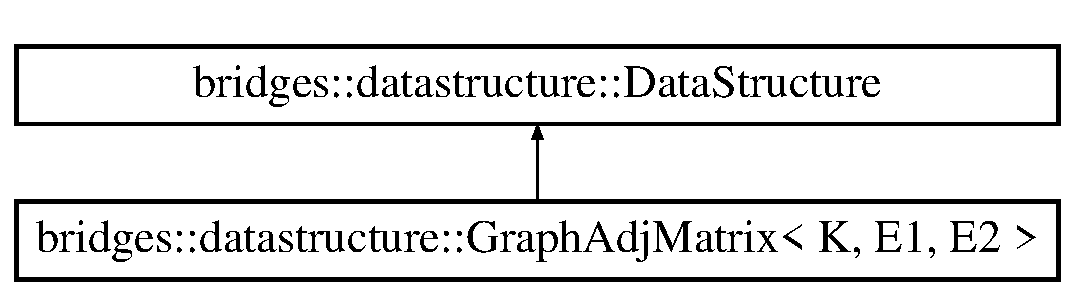
\includegraphics[height=2.000000cm]{classbridges_1_1datastructure_1_1_graph_adj_matrix}
\end{center}
\end{figure}


\subsection{Detailed Description}
\subsubsection*{template$<$typename K, typename E1 = K, typename E2 = E1$>$\newline
class bridges\+::datastructure\+::\+Graph\+Adj\+Matrix$<$ K, E1, E2 $>$}

This class provides methods to represent adjacency matrix based graphs. 

The class is simply a wrapper around the C++ S\+TL unordered\+\_\+map class and thus derives all its operations from it. Given the use of operator overloading, the adjacency matrix implementation is almost identical to a normal array representation, except that any ordered type can be used to index into the matrix.

Since the adjacency matrix typically contains only a numerical value, we keep edge specific information in a separate map using a generic parameter for the type.

Generic Parameters\+: K that is used as an index, E1 information specific to graph vertices E2 information specific to graph edges

\begin{DoxyAuthor}{Author}
Kalpathi Subramanian, Dakota Carmer 
\end{DoxyAuthor}
\begin{DoxyDate}{Date}
6/29/15, 7/10/16, 11/27/16, 4/22/18
\end{DoxyDate}
There is a tutorial about Graph Adjacency Matrix \+: \href{http://bridgesuncc.github.io/tutorials/Graph_AM.html}{\texttt{ http\+://bridgesuncc.\+github.\+io/tutorials/\+Graph\+\_\+\+A\+M.\+html}} \subsection*{Public Member Functions}
\begin{DoxyCompactItemize}
\item 
virtual const string \mbox{\hyperlink{classbridges_1_1datastructure_1_1_graph_adj_matrix_a2f8c67da1078354156fc646097152c6d}{get\+D\+Stype}} () const override
\item 
void \mbox{\hyperlink{classbridges_1_1datastructure_1_1_graph_adj_matrix_aaebb2607d06b1c36548652dba0211744}{add\+Vertex}} (const K \&k, const E1 \&e=E1())
\item 
void \mbox{\hyperlink{classbridges_1_1datastructure_1_1_graph_adj_matrix_ab23870ac203b3784157ecb05443494a4}{add\+Edge}} (const K \&src, const K \&dest, const unsigned int \&wt)
\item 
const unordered\+\_\+map$<$ K, unordered\+\_\+map$<$ K, int $>$ $>$ \& \mbox{\hyperlink{classbridges_1_1datastructure_1_1_graph_adj_matrix_aaf5c1ae5267b7ff4c8fcc861221ff2e8}{get\+Matrix}} () const
\item 
const unordered\+\_\+map$<$ K, int $>$ \& \mbox{\hyperlink{classbridges_1_1datastructure_1_1_graph_adj_matrix_a0b49749793278a1910dd5ea67dbaeacf}{get\+Matrix}} (K key) const
\item 
unordered\+\_\+map$<$ K, \mbox{\hyperlink{classbridges_1_1datastructure_1_1_element}{Element}}$<$ E1 $>$ $\ast$ $>$ $\ast$ \mbox{\hyperlink{classbridges_1_1datastructure_1_1_graph_adj_matrix_a4bcf803c43af2f14224a0891b9260fbf}{get\+Vertices}} ()
\item 
const \mbox{\hyperlink{classbridges_1_1datastructure_1_1_element}{Element}}$<$ E1 $>$ $\ast$ \mbox{\hyperlink{classbridges_1_1datastructure_1_1_graph_adj_matrix_a3de2ef8ce16e0c0d2240a92838ffd8aa}{get\+Vertex}} (const K \&key) const
\item 
\mbox{\hyperlink{classbridges_1_1datastructure_1_1_element}{Element}}$<$ E1 $>$ $\ast$ \mbox{\hyperlink{classbridges_1_1datastructure_1_1_graph_adj_matrix_a4100f224c05a77dd2c362c05fa15e6a2}{get\+Vertex}} (const K \&key)
\item 
E1 \mbox{\hyperlink{classbridges_1_1datastructure_1_1_graph_adj_matrix_a0be12527de2ab43b9de9b7ccd6e94d94}{get\+Vertex\+Data}} (const K \&src)
\item 
void \mbox{\hyperlink{classbridges_1_1datastructure_1_1_graph_adj_matrix_a8fb501cd1b1953c85e2aa3963f8ecd1f}{set\+Vertex\+Data}} (const K \&v\+ID, const E1 \&data)
\item 
E2 const  \& \mbox{\hyperlink{classbridges_1_1datastructure_1_1_graph_adj_matrix_ab6cd22b1a8f1e9f1c0865ba7aec6c6ca}{get\+Edge\+Data}} (const K \&src, const K \&dest) const
\item 
void \mbox{\hyperlink{classbridges_1_1datastructure_1_1_graph_adj_matrix_a9367d6bee5ce194bad2c8ca105d5be2f}{set\+Edge\+Data}} (const K \&src, const K \&dest, const E2 \&data)
\begin{DoxyCompactList}\small\item\em Loads edge information. \end{DoxyCompactList}\item 
\mbox{\hyperlink{classbridges_1_1datastructure_1_1_element_visualizer}{Element\+Visualizer}} $\ast$ \mbox{\hyperlink{classbridges_1_1datastructure_1_1_graph_adj_matrix_ad17ebd77b7fd42bd440aa5bbf313c752}{get\+Visualizer}} (const K \&k)
\item 
\mbox{\hyperlink{classbridges_1_1datastructure_1_1_link_visualizer}{Link\+Visualizer}} $\ast$ \mbox{\hyperlink{classbridges_1_1datastructure_1_1_graph_adj_matrix_ab41a062af77b11e5cc034f7c21d12421}{get\+Link\+Visualizer}} (const K \&k1, const K \&k2)
\end{DoxyCompactItemize}


\subsection{Member Function Documentation}
\mbox{\Hypertarget{classbridges_1_1datastructure_1_1_graph_adj_matrix_ab23870ac203b3784157ecb05443494a4}\label{classbridges_1_1datastructure_1_1_graph_adj_matrix_ab23870ac203b3784157ecb05443494a4}} 
\index{bridges::datastructure::GraphAdjMatrix$<$ K, E1, E2 $>$@{bridges::datastructure::GraphAdjMatrix$<$ K, E1, E2 $>$}!addEdge@{addEdge}}
\index{addEdge@{addEdge}!bridges::datastructure::GraphAdjMatrix$<$ K, E1, E2 $>$@{bridges::datastructure::GraphAdjMatrix$<$ K, E1, E2 $>$}}
\subsubsection{\texorpdfstring{addEdge()}{addEdge()}}
{\footnotesize\ttfamily template$<$typename K , typename E1  = K, typename E2  = E1$>$ \\
void \mbox{\hyperlink{classbridges_1_1datastructure_1_1_graph_adj_matrix}{bridges\+::datastructure\+::\+Graph\+Adj\+Matrix}}$<$ K, E1, E2 $>$\+::add\+Edge (\begin{DoxyParamCaption}\item[{const K \&}]{src,  }\item[{const K \&}]{dest,  }\item[{const unsigned int \&}]{wt }\end{DoxyParamCaption})\hspace{0.3cm}{\ttfamily [inline]}}

Sets the weight of the edge from \char`\"{}src\char`\"{} to \char`\"{}dest\char`\"{}, to \char`\"{}wt\char`\"{}. This will overwrite the existing edge weight.


\begin{DoxyParams}{Parameters}
{\em src} & The key of the source Vertex \\
\hline
{\em dest} & The key of the destination Vertex \\
\hline
{\em wt} & The weight of the edge \\
\hline
\end{DoxyParams}

\begin{DoxyExceptions}{Exceptions}
{\em out\+\_\+of\+\_\+range} & If \char`\"{}src\char`\"{} or \char`\"{}dest\char`\"{} is non-\/existent within this graph \\
\hline
\end{DoxyExceptions}
\mbox{\Hypertarget{classbridges_1_1datastructure_1_1_graph_adj_matrix_aaebb2607d06b1c36548652dba0211744}\label{classbridges_1_1datastructure_1_1_graph_adj_matrix_aaebb2607d06b1c36548652dba0211744}} 
\index{bridges::datastructure::GraphAdjMatrix$<$ K, E1, E2 $>$@{bridges::datastructure::GraphAdjMatrix$<$ K, E1, E2 $>$}!addVertex@{addVertex}}
\index{addVertex@{addVertex}!bridges::datastructure::GraphAdjMatrix$<$ K, E1, E2 $>$@{bridges::datastructure::GraphAdjMatrix$<$ K, E1, E2 $>$}}
\subsubsection{\texorpdfstring{addVertex()}{addVertex()}}
{\footnotesize\ttfamily template$<$typename K , typename E1  = K, typename E2  = E1$>$ \\
void \mbox{\hyperlink{classbridges_1_1datastructure_1_1_graph_adj_matrix}{bridges\+::datastructure\+::\+Graph\+Adj\+Matrix}}$<$ K, E1, E2 $>$\+::add\+Vertex (\begin{DoxyParamCaption}\item[{const K \&}]{k,  }\item[{const E1 \&}]{e = {\ttfamily E1()} }\end{DoxyParamCaption})\hspace{0.3cm}{\ttfamily [inline]}}

Adds a vertex of key \char`\"{}k\char`\"{} and value \char`\"{}e\char`\"{} to the graph. Sets all of its edges to be of weight 0.


\begin{DoxyParams}{Parameters}
{\em k} & Vertex key \\
\hline
{\em e} & Vertex data \\
\hline
\end{DoxyParams}
\mbox{\Hypertarget{classbridges_1_1datastructure_1_1_graph_adj_matrix_a2f8c67da1078354156fc646097152c6d}\label{classbridges_1_1datastructure_1_1_graph_adj_matrix_a2f8c67da1078354156fc646097152c6d}} 
\index{bridges::datastructure::GraphAdjMatrix$<$ K, E1, E2 $>$@{bridges::datastructure::GraphAdjMatrix$<$ K, E1, E2 $>$}!getDStype@{getDStype}}
\index{getDStype@{getDStype}!bridges::datastructure::GraphAdjMatrix$<$ K, E1, E2 $>$@{bridges::datastructure::GraphAdjMatrix$<$ K, E1, E2 $>$}}
\subsubsection{\texorpdfstring{getDStype()}{getDStype()}}
{\footnotesize\ttfamily template$<$typename K , typename E1  = K, typename E2  = E1$>$ \\
virtual const string \mbox{\hyperlink{classbridges_1_1datastructure_1_1_graph_adj_matrix}{bridges\+::datastructure\+::\+Graph\+Adj\+Matrix}}$<$ K, E1, E2 $>$\+::get\+D\+Stype (\begin{DoxyParamCaption}{ }\end{DoxyParamCaption}) const\hspace{0.3cm}{\ttfamily [inline]}, {\ttfamily [override]}, {\ttfamily [virtual]}}

\begin{DoxyReturn}{Returns}
The string representation of this data structure type 
\end{DoxyReturn}


Implements \mbox{\hyperlink{classbridges_1_1datastructure_1_1_data_structure_a4ff66cb34409f11fe9fc647f6d8a22ce}{bridges\+::datastructure\+::\+Data\+Structure}}.

\mbox{\Hypertarget{classbridges_1_1datastructure_1_1_graph_adj_matrix_ab6cd22b1a8f1e9f1c0865ba7aec6c6ca}\label{classbridges_1_1datastructure_1_1_graph_adj_matrix_ab6cd22b1a8f1e9f1c0865ba7aec6c6ca}} 
\index{bridges::datastructure::GraphAdjMatrix$<$ K, E1, E2 $>$@{bridges::datastructure::GraphAdjMatrix$<$ K, E1, E2 $>$}!getEdgeData@{getEdgeData}}
\index{getEdgeData@{getEdgeData}!bridges::datastructure::GraphAdjMatrix$<$ K, E1, E2 $>$@{bridges::datastructure::GraphAdjMatrix$<$ K, E1, E2 $>$}}
\subsubsection{\texorpdfstring{getEdgeData()}{getEdgeData()}}
{\footnotesize\ttfamily template$<$typename K , typename E1  = K, typename E2  = E1$>$ \\
E2 const\& \mbox{\hyperlink{classbridges_1_1datastructure_1_1_graph_adj_matrix}{bridges\+::datastructure\+::\+Graph\+Adj\+Matrix}}$<$ K, E1, E2 $>$\+::get\+Edge\+Data (\begin{DoxyParamCaption}\item[{const K \&}]{src,  }\item[{const K \&}]{dest }\end{DoxyParamCaption}) const\hspace{0.3cm}{\ttfamily [inline]}}

\begin{DoxyVerb}Gets edge data for the edge from "src" to "dest"
\end{DoxyVerb}



\begin{DoxyParams}{Parameters}
{\em src} & The key of the source Vertex \\
\hline
{\em dest} & The key of the destination Vertex\\
\hline
\end{DoxyParams}
\begin{DoxyReturn}{Returns}
edge specific data 
\end{DoxyReturn}
\mbox{\Hypertarget{classbridges_1_1datastructure_1_1_graph_adj_matrix_ab41a062af77b11e5cc034f7c21d12421}\label{classbridges_1_1datastructure_1_1_graph_adj_matrix_ab41a062af77b11e5cc034f7c21d12421}} 
\index{bridges::datastructure::GraphAdjMatrix$<$ K, E1, E2 $>$@{bridges::datastructure::GraphAdjMatrix$<$ K, E1, E2 $>$}!getLinkVisualizer@{getLinkVisualizer}}
\index{getLinkVisualizer@{getLinkVisualizer}!bridges::datastructure::GraphAdjMatrix$<$ K, E1, E2 $>$@{bridges::datastructure::GraphAdjMatrix$<$ K, E1, E2 $>$}}
\subsubsection{\texorpdfstring{getLinkVisualizer()}{getLinkVisualizer()}}
{\footnotesize\ttfamily template$<$typename K , typename E1  = K, typename E2  = E1$>$ \\
\mbox{\hyperlink{classbridges_1_1datastructure_1_1_link_visualizer}{Link\+Visualizer}}$\ast$ \mbox{\hyperlink{classbridges_1_1datastructure_1_1_graph_adj_matrix}{bridges\+::datastructure\+::\+Graph\+Adj\+Matrix}}$<$ K, E1, E2 $>$\+::get\+Link\+Visualizer (\begin{DoxyParamCaption}\item[{const K \&}]{k1,  }\item[{const K \&}]{k2 }\end{DoxyParamCaption})\hspace{0.3cm}{\ttfamily [inline]}}

Returns the link visualizer corresponding to two graph nodes with an existing link; error returned if no link exists.


\begin{DoxyParams}{Parameters}
{\em k1} & The key of the link source vertex \\
\hline
{\em k2} & The key of the link destination vertex\\
\hline
\end{DoxyParams}
\begin{DoxyReturn}{Returns}
the visualizer that controls the attributes of this link 
\end{DoxyReturn}
\mbox{\Hypertarget{classbridges_1_1datastructure_1_1_graph_adj_matrix_aaf5c1ae5267b7ff4c8fcc861221ff2e8}\label{classbridges_1_1datastructure_1_1_graph_adj_matrix_aaf5c1ae5267b7ff4c8fcc861221ff2e8}} 
\index{bridges::datastructure::GraphAdjMatrix$<$ K, E1, E2 $>$@{bridges::datastructure::GraphAdjMatrix$<$ K, E1, E2 $>$}!getMatrix@{getMatrix}}
\index{getMatrix@{getMatrix}!bridges::datastructure::GraphAdjMatrix$<$ K, E1, E2 $>$@{bridges::datastructure::GraphAdjMatrix$<$ K, E1, E2 $>$}}
\subsubsection{\texorpdfstring{getMatrix()}{getMatrix()}\hspace{0.1cm}{\footnotesize\ttfamily [1/2]}}
{\footnotesize\ttfamily template$<$typename K , typename E1  = K, typename E2  = E1$>$ \\
const unordered\+\_\+map$<$K, unordered\+\_\+map$<$K, int$>$ $>$\& \mbox{\hyperlink{classbridges_1_1datastructure_1_1_graph_adj_matrix}{bridges\+::datastructure\+::\+Graph\+Adj\+Matrix}}$<$ K, E1, E2 $>$\+::get\+Matrix (\begin{DoxyParamCaption}{ }\end{DoxyParamCaption}) const\hspace{0.3cm}{\ttfamily [inline]}}

Return the adjacency matrix \begin{DoxyReturn}{Returns}
The matrix of this graphs edges 
\end{DoxyReturn}
\mbox{\Hypertarget{classbridges_1_1datastructure_1_1_graph_adj_matrix_a0b49749793278a1910dd5ea67dbaeacf}\label{classbridges_1_1datastructure_1_1_graph_adj_matrix_a0b49749793278a1910dd5ea67dbaeacf}} 
\index{bridges::datastructure::GraphAdjMatrix$<$ K, E1, E2 $>$@{bridges::datastructure::GraphAdjMatrix$<$ K, E1, E2 $>$}!getMatrix@{getMatrix}}
\index{getMatrix@{getMatrix}!bridges::datastructure::GraphAdjMatrix$<$ K, E1, E2 $>$@{bridges::datastructure::GraphAdjMatrix$<$ K, E1, E2 $>$}}
\subsubsection{\texorpdfstring{getMatrix()}{getMatrix()}\hspace{0.1cm}{\footnotesize\ttfamily [2/2]}}
{\footnotesize\ttfamily template$<$typename K , typename E1  = K, typename E2  = E1$>$ \\
const unordered\+\_\+map$<$K, int$>$\& \mbox{\hyperlink{classbridges_1_1datastructure_1_1_graph_adj_matrix}{bridges\+::datastructure\+::\+Graph\+Adj\+Matrix}}$<$ K, E1, E2 $>$\+::get\+Matrix (\begin{DoxyParamCaption}\item[{K}]{key }\end{DoxyParamCaption}) const\hspace{0.3cm}{\ttfamily [inline]}}

Return the adjacency matrix row at Key key 
\begin{DoxyParams}{Parameters}
{\em key} & The input key value that identifies the row being retrieved\\
\hline
\end{DoxyParams}
\begin{DoxyReturn}{Returns}
The row of this adjacency matrix corresponding to the key 
\end{DoxyReturn}
\mbox{\Hypertarget{classbridges_1_1datastructure_1_1_graph_adj_matrix_a3de2ef8ce16e0c0d2240a92838ffd8aa}\label{classbridges_1_1datastructure_1_1_graph_adj_matrix_a3de2ef8ce16e0c0d2240a92838ffd8aa}} 
\index{bridges::datastructure::GraphAdjMatrix$<$ K, E1, E2 $>$@{bridges::datastructure::GraphAdjMatrix$<$ K, E1, E2 $>$}!getVertex@{getVertex}}
\index{getVertex@{getVertex}!bridges::datastructure::GraphAdjMatrix$<$ K, E1, E2 $>$@{bridges::datastructure::GraphAdjMatrix$<$ K, E1, E2 $>$}}
\subsubsection{\texorpdfstring{getVertex()}{getVertex()}\hspace{0.1cm}{\footnotesize\ttfamily [1/2]}}
{\footnotesize\ttfamily template$<$typename K , typename E1  = K, typename E2  = E1$>$ \\
const \mbox{\hyperlink{classbridges_1_1datastructure_1_1_element}{Element}}$<$E1$>$$\ast$ \mbox{\hyperlink{classbridges_1_1datastructure_1_1_graph_adj_matrix}{bridges\+::datastructure\+::\+Graph\+Adj\+Matrix}}$<$ K, E1, E2 $>$\+::get\+Vertex (\begin{DoxyParamCaption}\item[{const K \&}]{key }\end{DoxyParamCaption}) const\hspace{0.3cm}{\ttfamily [inline]}}

Return the vertex correspondingto key \char`\"{}key\char`\"{} -\/ const version \begin{DoxyReturn}{Returns}
the requested vertex of this graph 
\end{DoxyReturn}
\mbox{\Hypertarget{classbridges_1_1datastructure_1_1_graph_adj_matrix_a4100f224c05a77dd2c362c05fa15e6a2}\label{classbridges_1_1datastructure_1_1_graph_adj_matrix_a4100f224c05a77dd2c362c05fa15e6a2}} 
\index{bridges::datastructure::GraphAdjMatrix$<$ K, E1, E2 $>$@{bridges::datastructure::GraphAdjMatrix$<$ K, E1, E2 $>$}!getVertex@{getVertex}}
\index{getVertex@{getVertex}!bridges::datastructure::GraphAdjMatrix$<$ K, E1, E2 $>$@{bridges::datastructure::GraphAdjMatrix$<$ K, E1, E2 $>$}}
\subsubsection{\texorpdfstring{getVertex()}{getVertex()}\hspace{0.1cm}{\footnotesize\ttfamily [2/2]}}
{\footnotesize\ttfamily template$<$typename K , typename E1  = K, typename E2  = E1$>$ \\
\mbox{\hyperlink{classbridges_1_1datastructure_1_1_element}{Element}}$<$E1$>$$\ast$ \mbox{\hyperlink{classbridges_1_1datastructure_1_1_graph_adj_matrix}{bridges\+::datastructure\+::\+Graph\+Adj\+Matrix}}$<$ K, E1, E2 $>$\+::get\+Vertex (\begin{DoxyParamCaption}\item[{const K \&}]{key }\end{DoxyParamCaption})\hspace{0.3cm}{\ttfamily [inline]}}

Return the vertex correspondingto key \char`\"{}key\char`\"{} \begin{DoxyReturn}{Returns}
the requested vertex of this graph 
\end{DoxyReturn}
\mbox{\Hypertarget{classbridges_1_1datastructure_1_1_graph_adj_matrix_a0be12527de2ab43b9de9b7ccd6e94d94}\label{classbridges_1_1datastructure_1_1_graph_adj_matrix_a0be12527de2ab43b9de9b7ccd6e94d94}} 
\index{bridges::datastructure::GraphAdjMatrix$<$ K, E1, E2 $>$@{bridges::datastructure::GraphAdjMatrix$<$ K, E1, E2 $>$}!getVertexData@{getVertexData}}
\index{getVertexData@{getVertexData}!bridges::datastructure::GraphAdjMatrix$<$ K, E1, E2 $>$@{bridges::datastructure::GraphAdjMatrix$<$ K, E1, E2 $>$}}
\subsubsection{\texorpdfstring{getVertexData()}{getVertexData()}}
{\footnotesize\ttfamily template$<$typename K , typename E1  = K, typename E2  = E1$>$ \\
E1 \mbox{\hyperlink{classbridges_1_1datastructure_1_1_graph_adj_matrix}{bridges\+::datastructure\+::\+Graph\+Adj\+Matrix}}$<$ K, E1, E2 $>$\+::get\+Vertex\+Data (\begin{DoxyParamCaption}\item[{const K \&}]{src }\end{DoxyParamCaption})\hspace{0.3cm}{\ttfamily [inline]}}

Gets vertex data for a graph vertex


\begin{DoxyParams}{Parameters}
{\em src} & The key of the source vertex\\
\hline
\end{DoxyParams}
\begin{DoxyReturn}{Returns}
E vertex specific data 
\end{DoxyReturn}
\mbox{\Hypertarget{classbridges_1_1datastructure_1_1_graph_adj_matrix_a4bcf803c43af2f14224a0891b9260fbf}\label{classbridges_1_1datastructure_1_1_graph_adj_matrix_a4bcf803c43af2f14224a0891b9260fbf}} 
\index{bridges::datastructure::GraphAdjMatrix$<$ K, E1, E2 $>$@{bridges::datastructure::GraphAdjMatrix$<$ K, E1, E2 $>$}!getVertices@{getVertices}}
\index{getVertices@{getVertices}!bridges::datastructure::GraphAdjMatrix$<$ K, E1, E2 $>$@{bridges::datastructure::GraphAdjMatrix$<$ K, E1, E2 $>$}}
\subsubsection{\texorpdfstring{getVertices()}{getVertices()}}
{\footnotesize\ttfamily template$<$typename K , typename E1  = K, typename E2  = E1$>$ \\
unordered\+\_\+map$<$K, \mbox{\hyperlink{classbridges_1_1datastructure_1_1_element}{Element}}$<$E1$>$ $\ast$$>$$\ast$ \mbox{\hyperlink{classbridges_1_1datastructure_1_1_graph_adj_matrix}{bridges\+::datastructure\+::\+Graph\+Adj\+Matrix}}$<$ K, E1, E2 $>$\+::get\+Vertices (\begin{DoxyParamCaption}{ }\end{DoxyParamCaption})\hspace{0.3cm}{\ttfamily [inline]}}

Return the graph vertices \begin{DoxyReturn}{Returns}
The graph verticies 
\end{DoxyReturn}
\mbox{\Hypertarget{classbridges_1_1datastructure_1_1_graph_adj_matrix_ad17ebd77b7fd42bd440aa5bbf313c752}\label{classbridges_1_1datastructure_1_1_graph_adj_matrix_ad17ebd77b7fd42bd440aa5bbf313c752}} 
\index{bridges::datastructure::GraphAdjMatrix$<$ K, E1, E2 $>$@{bridges::datastructure::GraphAdjMatrix$<$ K, E1, E2 $>$}!getVisualizer@{getVisualizer}}
\index{getVisualizer@{getVisualizer}!bridges::datastructure::GraphAdjMatrix$<$ K, E1, E2 $>$@{bridges::datastructure::GraphAdjMatrix$<$ K, E1, E2 $>$}}
\subsubsection{\texorpdfstring{getVisualizer()}{getVisualizer()}}
{\footnotesize\ttfamily template$<$typename K , typename E1  = K, typename E2  = E1$>$ \\
\mbox{\hyperlink{classbridges_1_1datastructure_1_1_element_visualizer}{Element\+Visualizer}}$\ast$ \mbox{\hyperlink{classbridges_1_1datastructure_1_1_graph_adj_matrix}{bridges\+::datastructure\+::\+Graph\+Adj\+Matrix}}$<$ K, E1, E2 $>$\+::get\+Visualizer (\begin{DoxyParamCaption}\item[{const K \&}]{k }\end{DoxyParamCaption})\hspace{0.3cm}{\ttfamily [inline]}}

Returns the visualizer corresponding to a graph vertex; convenient method to set attributes of the graph vertex


\begin{DoxyParams}{Parameters}
{\em k} & The key of the graph vertex\\
\hline
\end{DoxyParams}
\begin{DoxyReturn}{Returns}
the visualizer that controls the attributes of this node 
\end{DoxyReturn}
\mbox{\Hypertarget{classbridges_1_1datastructure_1_1_graph_adj_matrix_a9367d6bee5ce194bad2c8ca105d5be2f}\label{classbridges_1_1datastructure_1_1_graph_adj_matrix_a9367d6bee5ce194bad2c8ca105d5be2f}} 
\index{bridges::datastructure::GraphAdjMatrix$<$ K, E1, E2 $>$@{bridges::datastructure::GraphAdjMatrix$<$ K, E1, E2 $>$}!setEdgeData@{setEdgeData}}
\index{setEdgeData@{setEdgeData}!bridges::datastructure::GraphAdjMatrix$<$ K, E1, E2 $>$@{bridges::datastructure::GraphAdjMatrix$<$ K, E1, E2 $>$}}
\subsubsection{\texorpdfstring{setEdgeData()}{setEdgeData()}}
{\footnotesize\ttfamily template$<$typename K , typename E1  = K, typename E2  = E1$>$ \\
void \mbox{\hyperlink{classbridges_1_1datastructure_1_1_graph_adj_matrix}{bridges\+::datastructure\+::\+Graph\+Adj\+Matrix}}$<$ K, E1, E2 $>$\+::set\+Edge\+Data (\begin{DoxyParamCaption}\item[{const K \&}]{src,  }\item[{const K \&}]{dest,  }\item[{const E2 \&}]{data }\end{DoxyParamCaption})\hspace{0.3cm}{\ttfamily [inline]}}



Loads edge information. 


\begin{DoxyParams}{Parameters}
{\em src} & The key of the source Vertex \\
\hline
{\em dest} & The key of the destination Vertex \\
\hline
{\em data} & data to associate with the edge \\
\hline
\end{DoxyParams}
\mbox{\Hypertarget{classbridges_1_1datastructure_1_1_graph_adj_matrix_a8fb501cd1b1953c85e2aa3963f8ecd1f}\label{classbridges_1_1datastructure_1_1_graph_adj_matrix_a8fb501cd1b1953c85e2aa3963f8ecd1f}} 
\index{bridges::datastructure::GraphAdjMatrix$<$ K, E1, E2 $>$@{bridges::datastructure::GraphAdjMatrix$<$ K, E1, E2 $>$}!setVertexData@{setVertexData}}
\index{setVertexData@{setVertexData}!bridges::datastructure::GraphAdjMatrix$<$ K, E1, E2 $>$@{bridges::datastructure::GraphAdjMatrix$<$ K, E1, E2 $>$}}
\subsubsection{\texorpdfstring{setVertexData()}{setVertexData()}}
{\footnotesize\ttfamily template$<$typename K , typename E1  = K, typename E2  = E1$>$ \\
void \mbox{\hyperlink{classbridges_1_1datastructure_1_1_graph_adj_matrix}{bridges\+::datastructure\+::\+Graph\+Adj\+Matrix}}$<$ K, E1, E2 $>$\+::set\+Vertex\+Data (\begin{DoxyParamCaption}\item[{const K \&}]{v\+ID,  }\item[{const E1 \&}]{data }\end{DoxyParamCaption})\hspace{0.3cm}{\ttfamily [inline]}}

\begin{DoxyVerb}Loads vertex specific information for a graph vertex
\end{DoxyVerb}



\begin{DoxyParams}{Parameters}
{\em v\+ID} & vertex key \\
\hline
{\em data} & data to associate with the vertex \\
\hline
\end{DoxyParams}


The documentation for this class was generated from the following files\+:\begin{DoxyCompactItemize}
\item 
/\+Users/kalpathi/gr/bridges/cxx/src/\mbox{\hyperlink{_element_8h}{Element.\+h}}\item 
/\+Users/kalpathi/gr/bridges/cxx/src/\mbox{\hyperlink{_graph_adj_matrix_8h}{Graph\+Adj\+Matrix.\+h}}\end{DoxyCompactItemize}

\hypertarget{classbridges_1_1benchmark_1_1_graph_benchmark}{}\doxysection{bridges\+::benchmark\+::Graph\+Benchmark Class Reference}
\label{classbridges_1_1benchmark_1_1_graph_benchmark}\index{bridges::benchmark::GraphBenchmark@{bridges::benchmark::GraphBenchmark}}


{\ttfamily \#include $<$Graph\+Benchmark.\+h$>$}

Inheritance diagram for bridges\+::benchmark\+::Graph\+Benchmark\+:\begin{figure}[H]
\begin{center}
\leavevmode
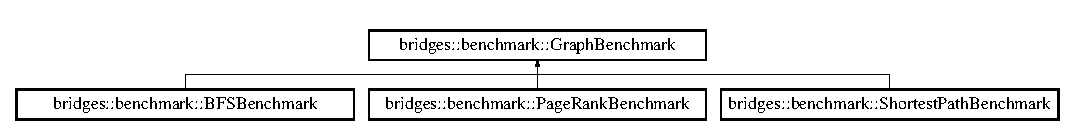
\includegraphics[height=1.382716cm]{classbridges_1_1benchmark_1_1_graph_benchmark}
\end{center}
\end{figure}


\doxysubsection{Detailed Description}
Base class for a variety of graph based benchmark. 

This class is not meant to be used directly by students. \doxysubsection*{Public Member Functions}
\begin{DoxyCompactItemize}
\item 
void \mbox{\hyperlink{classbridges_1_1benchmark_1_1_graph_benchmark_a56934eb2789e54c088e7b4423c3a7456}{set\+Time\+Cap}} (double cap\+\_\+in\+\_\+s)
\begin{DoxyCompactList}\small\item\em sets an upper bound to the time of a run. \end{DoxyCompactList}\item 
double \mbox{\hyperlink{classbridges_1_1benchmark_1_1_graph_benchmark_a2bfaccb0b170b831c1aa9776c0a64d72}{get\+Time\+Cap}} () const
\begin{DoxyCompactList}\small\item\em Return time limit of a run. \end{DoxyCompactList}\end{DoxyCompactItemize}
\doxysubsection*{Protected Member Functions}
\begin{DoxyCompactItemize}
\item 
\mbox{\hyperlink{classbridges_1_1benchmark_1_1_graph_benchmark_a617520fd2675b1ec03eb4eaf30affa9d}{Graph\+Benchmark}} ()
\item 
std\+::tuple$<$ long, long $>$ \mbox{\hyperlink{classbridges_1_1benchmark_1_1_graph_benchmark_a561d704a89e9e824cc6b246266cf05d7}{generate\+Wikidata\+Movie\+Actor}} (int yearmin, int yearmax, \mbox{\hyperlink{classbridges_1_1datastructure_1_1_graph_adj_list}{Graph\+Adj\+List}}$<$ std\+::string $>$ \&moviegraph)
\item 
std\+::string \mbox{\hyperlink{classbridges_1_1benchmark_1_1_graph_benchmark_a68b899e43ab8afc17cbca344004f65fb}{highest\+Degree\+Vertex}} (\mbox{\hyperlink{classbridges_1_1datastructure_1_1_graph_adj_list}{Graph\+Adj\+List}}$<$ std\+::string $>$ \&gr)
\item 
{\footnotesize template$<$typename Graph\+Type $>$ }\\long \mbox{\hyperlink{classbridges_1_1benchmark_1_1_graph_benchmark_aa8496248acdb735f170f46ee66bdb4ce}{count\+Vertices}} (const Graph\+Type \&gr)
\item 
{\footnotesize template$<$typename Graph\+Type $>$ }\\long \mbox{\hyperlink{classbridges_1_1benchmark_1_1_graph_benchmark_a18fc383926e9067fc98506449c819d22}{count\+Edges}} (const Graph\+Type \&gr)
\end{DoxyCompactItemize}
\doxysubsection*{Protected Attributes}
\begin{DoxyCompactItemize}
\item 
double \mbox{\hyperlink{classbridges_1_1benchmark_1_1_graph_benchmark_a59938016b721fb6db2ff8bdb2c9d41c1}{time\+\_\+cap}}
\end{DoxyCompactItemize}


\doxysubsection{Constructor \& Destructor Documentation}
\mbox{\Hypertarget{classbridges_1_1benchmark_1_1_graph_benchmark_a617520fd2675b1ec03eb4eaf30affa9d}\label{classbridges_1_1benchmark_1_1_graph_benchmark_a617520fd2675b1ec03eb4eaf30affa9d}} 
\index{bridges::benchmark::GraphBenchmark@{bridges::benchmark::GraphBenchmark}!GraphBenchmark@{GraphBenchmark}}
\index{GraphBenchmark@{GraphBenchmark}!bridges::benchmark::GraphBenchmark@{bridges::benchmark::GraphBenchmark}}
\doxysubsubsection{\texorpdfstring{GraphBenchmark()}{GraphBenchmark()}}
{\footnotesize\ttfamily bridges\+::benchmark\+::\+Graph\+Benchmark\+::\+Graph\+Benchmark (\begin{DoxyParamCaption}{ }\end{DoxyParamCaption})\hspace{0.3cm}{\ttfamily [inline]}, {\ttfamily [protected]}}



\doxysubsection{Member Function Documentation}
\mbox{\Hypertarget{classbridges_1_1benchmark_1_1_graph_benchmark_a18fc383926e9067fc98506449c819d22}\label{classbridges_1_1benchmark_1_1_graph_benchmark_a18fc383926e9067fc98506449c819d22}} 
\index{bridges::benchmark::GraphBenchmark@{bridges::benchmark::GraphBenchmark}!countEdges@{countEdges}}
\index{countEdges@{countEdges}!bridges::benchmark::GraphBenchmark@{bridges::benchmark::GraphBenchmark}}
\doxysubsubsection{\texorpdfstring{countEdges()}{countEdges()}}
{\footnotesize\ttfamily template$<$typename Graph\+Type $>$ \\
long bridges\+::benchmark\+::\+Graph\+Benchmark\+::count\+Edges (\begin{DoxyParamCaption}\item[{const Graph\+Type \&}]{gr }\end{DoxyParamCaption})\hspace{0.3cm}{\ttfamily [inline]}, {\ttfamily [protected]}}

\mbox{\Hypertarget{classbridges_1_1benchmark_1_1_graph_benchmark_aa8496248acdb735f170f46ee66bdb4ce}\label{classbridges_1_1benchmark_1_1_graph_benchmark_aa8496248acdb735f170f46ee66bdb4ce}} 
\index{bridges::benchmark::GraphBenchmark@{bridges::benchmark::GraphBenchmark}!countVertices@{countVertices}}
\index{countVertices@{countVertices}!bridges::benchmark::GraphBenchmark@{bridges::benchmark::GraphBenchmark}}
\doxysubsubsection{\texorpdfstring{countVertices()}{countVertices()}}
{\footnotesize\ttfamily template$<$typename Graph\+Type $>$ \\
long bridges\+::benchmark\+::\+Graph\+Benchmark\+::count\+Vertices (\begin{DoxyParamCaption}\item[{const Graph\+Type \&}]{gr }\end{DoxyParamCaption})\hspace{0.3cm}{\ttfamily [inline]}, {\ttfamily [protected]}}

\mbox{\Hypertarget{classbridges_1_1benchmark_1_1_graph_benchmark_a561d704a89e9e824cc6b246266cf05d7}\label{classbridges_1_1benchmark_1_1_graph_benchmark_a561d704a89e9e824cc6b246266cf05d7}} 
\index{bridges::benchmark::GraphBenchmark@{bridges::benchmark::GraphBenchmark}!generateWikidataMovieActor@{generateWikidataMovieActor}}
\index{generateWikidataMovieActor@{generateWikidataMovieActor}!bridges::benchmark::GraphBenchmark@{bridges::benchmark::GraphBenchmark}}
\doxysubsubsection{\texorpdfstring{generateWikidataMovieActor()}{generateWikidataMovieActor()}}
{\footnotesize\ttfamily std\+::tuple$<$long, long$>$ bridges\+::benchmark\+::\+Graph\+Benchmark\+::generate\+Wikidata\+Movie\+Actor (\begin{DoxyParamCaption}\item[{int}]{yearmin,  }\item[{int}]{yearmax,  }\item[{\mbox{\hyperlink{classbridges_1_1datastructure_1_1_graph_adj_list}{Graph\+Adj\+List}}$<$ std\+::string $>$ \&}]{moviegraph }\end{DoxyParamCaption})\hspace{0.3cm}{\ttfamily [inline]}, {\ttfamily [protected]}}

\begin{DoxyReturn}{Returns}
a triplet\+: the graph, the number of vertices, and the number of edges 
\end{DoxyReturn}
\mbox{\Hypertarget{classbridges_1_1benchmark_1_1_graph_benchmark_a2bfaccb0b170b831c1aa9776c0a64d72}\label{classbridges_1_1benchmark_1_1_graph_benchmark_a2bfaccb0b170b831c1aa9776c0a64d72}} 
\index{bridges::benchmark::GraphBenchmark@{bridges::benchmark::GraphBenchmark}!getTimeCap@{getTimeCap}}
\index{getTimeCap@{getTimeCap}!bridges::benchmark::GraphBenchmark@{bridges::benchmark::GraphBenchmark}}
\doxysubsubsection{\texorpdfstring{getTimeCap()}{getTimeCap()}}
{\footnotesize\ttfamily double bridges\+::benchmark\+::\+Graph\+Benchmark\+::get\+Time\+Cap (\begin{DoxyParamCaption}{ }\end{DoxyParamCaption}) const\hspace{0.3cm}{\ttfamily [inline]}}



Return time limit of a run. 

The benchmark will end after a run if it takes more than the given amount of time. So it is possible a particular run takes more than the alloted time, but that will be the last run.

\begin{DoxyReturn}{Returns}
the time upper bound (in seconds) of a particular run. 
\end{DoxyReturn}
\mbox{\Hypertarget{classbridges_1_1benchmark_1_1_graph_benchmark_a68b899e43ab8afc17cbca344004f65fb}\label{classbridges_1_1benchmark_1_1_graph_benchmark_a68b899e43ab8afc17cbca344004f65fb}} 
\index{bridges::benchmark::GraphBenchmark@{bridges::benchmark::GraphBenchmark}!highestDegreeVertex@{highestDegreeVertex}}
\index{highestDegreeVertex@{highestDegreeVertex}!bridges::benchmark::GraphBenchmark@{bridges::benchmark::GraphBenchmark}}
\doxysubsubsection{\texorpdfstring{highestDegreeVertex()}{highestDegreeVertex()}}
{\footnotesize\ttfamily std\+::string bridges\+::benchmark\+::\+Graph\+Benchmark\+::highest\+Degree\+Vertex (\begin{DoxyParamCaption}\item[{\mbox{\hyperlink{classbridges_1_1datastructure_1_1_graph_adj_list}{Graph\+Adj\+List}}$<$ std\+::string $>$ \&}]{gr }\end{DoxyParamCaption})\hspace{0.3cm}{\ttfamily [inline]}, {\ttfamily [protected]}}

\mbox{\Hypertarget{classbridges_1_1benchmark_1_1_graph_benchmark_a56934eb2789e54c088e7b4423c3a7456}\label{classbridges_1_1benchmark_1_1_graph_benchmark_a56934eb2789e54c088e7b4423c3a7456}} 
\index{bridges::benchmark::GraphBenchmark@{bridges::benchmark::GraphBenchmark}!setTimeCap@{setTimeCap}}
\index{setTimeCap@{setTimeCap}!bridges::benchmark::GraphBenchmark@{bridges::benchmark::GraphBenchmark}}
\doxysubsubsection{\texorpdfstring{setTimeCap()}{setTimeCap()}}
{\footnotesize\ttfamily void bridges\+::benchmark\+::\+Graph\+Benchmark\+::set\+Time\+Cap (\begin{DoxyParamCaption}\item[{double}]{cap\+\_\+in\+\_\+s }\end{DoxyParamCaption})\hspace{0.3cm}{\ttfamily [inline]}}



sets an upper bound to the time of a run. 

The benchmark will end after a run if it takes more than the given amount of time. So it is possible a particular run takes more than the alloted time, but that will be the last run.


\begin{DoxyParams}{Parameters}
{\em cap\+\_\+in\+\_\+s} & time limit in seconds \\
\hline
\end{DoxyParams}


\doxysubsection{Member Data Documentation}
\mbox{\Hypertarget{classbridges_1_1benchmark_1_1_graph_benchmark_a59938016b721fb6db2ff8bdb2c9d41c1}\label{classbridges_1_1benchmark_1_1_graph_benchmark_a59938016b721fb6db2ff8bdb2c9d41c1}} 
\index{bridges::benchmark::GraphBenchmark@{bridges::benchmark::GraphBenchmark}!time\_cap@{time\_cap}}
\index{time\_cap@{time\_cap}!bridges::benchmark::GraphBenchmark@{bridges::benchmark::GraphBenchmark}}
\doxysubsubsection{\texorpdfstring{time\_cap}{time\_cap}}
{\footnotesize\ttfamily double bridges\+::benchmark\+::\+Graph\+Benchmark\+::time\+\_\+cap\hspace{0.3cm}{\ttfamily [protected]}}



The documentation for this class was generated from the following file\+:\begin{DoxyCompactItemize}
\item 
/home/erik/work/bridges/bridges-\/cxx/src/\mbox{\hyperlink{_graph_benchmark_8h}{Graph\+Benchmark.\+h}}\end{DoxyCompactItemize}

\hypertarget{classbridges_1_1datastructure_1_1_grid}{}\section{bridges\+:\+:datastructure\+:\+:Grid$<$ E $>$ Class Template Reference}
\label{classbridges_1_1datastructure_1_1_grid}\index{bridges\+::datastructure\+::\+Grid$<$ E $>$@{bridges\+::datastructure\+::\+Grid$<$ E $>$}}


{\ttfamily \#include $<$Grid.\+h$>$}

Inheritance diagram for bridges\+:\+:datastructure\+:\+:Grid$<$ E $>$\+:\begin{figure}[H]
\begin{center}
\leavevmode
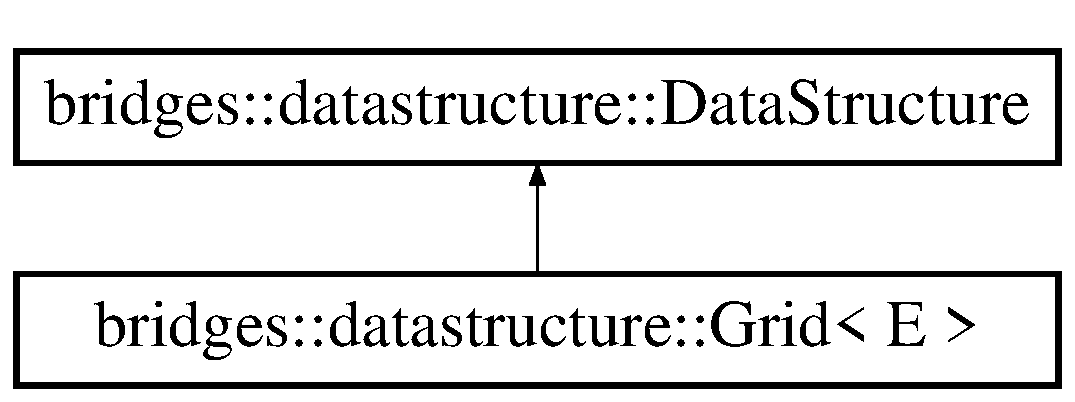
\includegraphics[height=2.000000cm]{classbridges_1_1datastructure_1_1_grid}
\end{center}
\end{figure}


\subsection{Detailed Description}
\subsubsection*{template$<$typename E$>$\newline
class bridges\+::datastructure\+::\+Grid$<$ E $>$}

This is a class in B\+R\+I\+D\+G\+ES for representing an (n x n) grid. 

This class will be useful in applications such as image processing, board games, etc.

\begin{DoxyAuthor}{Author}
David Burlinson, C++ port Kalpathi Subramanian 
\end{DoxyAuthor}
\begin{DoxyDate}{Date}
7/12/19
\end{DoxyDate}

\begin{DoxyParams}{Parameters}
{\em E} & There is a tutorial about \mbox{\hyperlink{classbridges_1_1datastructure_1_1_grid}{Grid}} \+: \href{http://bridgesuncc.github.io/tutorials/Grid.html}{\tt http\+://bridgesuncc.\+github.\+io/tutorials/\+Grid.\+html} \\
\hline
\end{DoxyParams}
\subsection*{Classes}
\begin{DoxyCompactItemize}
\item 
class \mbox{\hyperlink{classbridges_1_1datastructure_1_1_grid_1_1_bracket_helper}{Bracket\+Helper}}
\item 
class \mbox{\hyperlink{classbridges_1_1datastructure_1_1_grid_1_1_bracket_helper_const}{Bracket\+Helper\+Const}}
\end{DoxyCompactItemize}
\subsection*{Public Member Functions}
\begin{DoxyCompactItemize}
\item 
virtual const string \mbox{\hyperlink{classbridges_1_1datastructure_1_1_grid_a16aeae38446b96f440dea15f2b19334d}{get\+D\+Stype}} () const override
\item 
\mbox{\hyperlink{classbridges_1_1datastructure_1_1_grid_a80d8bca9d3793d896a92168a54ce7b2b}{Grid}} (int rows, int cols)
\item 
\mbox{\hyperlink{classbridges_1_1datastructure_1_1_grid_a41c8c94cd9a22ccf978c5e2b1141c813}{Grid}} ()
\item 
\mbox{\hyperlink{classbridges_1_1datastructure_1_1_grid_ad47ddbed7bbd07f98aaa61b74fcf826c}{Grid}} (int $\ast$size)
\item 
\mbox{\hyperlink{classbridges_1_1datastructure_1_1_grid_afc81003993a30d1112d2dff71bfc191b}{Grid}} (const \mbox{\hyperlink{classbridges_1_1datastructure_1_1_grid}{Grid}} \&g)
\item 
virtual \mbox{\hyperlink{classbridges_1_1datastructure_1_1_grid_aa04b4929a35fa359dbaab86e46fda204}{$\sim$\+Grid}} ()
\item 
\mbox{\hyperlink{classbridges_1_1datastructure_1_1_grid}{Grid}} \& \mbox{\hyperlink{classbridges_1_1datastructure_1_1_grid_a3522d8c94ad390ebafb12257a6c9b82f}{operator=}} (const \mbox{\hyperlink{classbridges_1_1datastructure_1_1_grid}{Grid}} \&g)
\item 
void \mbox{\hyperlink{classbridges_1_1datastructure_1_1_grid_a234818a9e22b6cefe943210c088c2a76}{set\+Dimensions}} (int rows, int cols)
\item 
int const  $\ast$ \mbox{\hyperlink{classbridges_1_1datastructure_1_1_grid_a5f1427f96782b3667585c06caef0b533}{get\+Dimensions}} ()
\item 
E const  \& \mbox{\hyperlink{classbridges_1_1datastructure_1_1_grid_a1ff40a322e0c6407affb608366f895b6}{get}} (int row, int col) const
\item 
void \mbox{\hyperlink{classbridges_1_1datastructure_1_1_grid_ac0d4784a31f69d8cf4be38952730cfa8}{set}} (int row, int col, E val)
\item 
\mbox{\hyperlink{classbridges_1_1datastructure_1_1_grid_1_1_bracket_helper_const}{Bracket\+Helper\+Const}} \mbox{\hyperlink{classbridges_1_1datastructure_1_1_grid_a754a890728b6b268a1ba843da89cb1f6}{operator\mbox{[}$\,$\mbox{]}}} (int row) const
\begin{DoxyCompactList}\small\item\em provides the necessary abstraction to do something = grid\mbox{[}x\mbox{]}\mbox{[}y\mbox{]}; \end{DoxyCompactList}\item 
\mbox{\hyperlink{classbridges_1_1datastructure_1_1_grid_1_1_bracket_helper}{Bracket\+Helper}} \mbox{\hyperlink{classbridges_1_1datastructure_1_1_grid_ae5a7cf159c7918193ba75146660c3c1f}{operator\mbox{[}$\,$\mbox{]}}} (int row)
\begin{DoxyCompactList}\small\item\em provides the necessary abstraction to do grid\mbox{[}x\mbox{]}\mbox{[}y\mbox{]} = something; \end{DoxyCompactList}\end{DoxyCompactItemize}
\subsection*{Protected Attributes}
\begin{DoxyCompactItemize}
\item 
E $\ast$$\ast$ \mbox{\hyperlink{classbridges_1_1datastructure_1_1_grid_aa29a07fad530eacd55e6244471ec4ecb}{grid}} = nullptr
\item 
int \mbox{\hyperlink{classbridges_1_1datastructure_1_1_grid_a97738e6230af3e7e593e93ecfde0b731}{grid\+Size}} \mbox{[}2\mbox{]}
\item 
int \mbox{\hyperlink{classbridges_1_1datastructure_1_1_grid_acb1cca7db5fb42a0b107885f9e00ff67}{max\+Grid\+Size}} \mbox{[}2\mbox{]} = \{1080, 1920\}
\end{DoxyCompactItemize}


\subsection{Constructor \& Destructor Documentation}
\mbox{\Hypertarget{classbridges_1_1datastructure_1_1_grid_a80d8bca9d3793d896a92168a54ce7b2b}\label{classbridges_1_1datastructure_1_1_grid_a80d8bca9d3793d896a92168a54ce7b2b}} 
\index{bridges\+::datastructure\+::\+Grid@{bridges\+::datastructure\+::\+Grid}!Grid@{Grid}}
\index{Grid@{Grid}!bridges\+::datastructure\+::\+Grid@{bridges\+::datastructure\+::\+Grid}}
\subsubsection{\texorpdfstring{Grid()}{Grid()}\hspace{0.1cm}{\footnotesize\ttfamily [1/4]}}
{\footnotesize\ttfamily template$<$typename E$>$ \\
\mbox{\hyperlink{classbridges_1_1datastructure_1_1_grid}{bridges\+::datastructure\+::\+Grid}}$<$ E $>$\+::\mbox{\hyperlink{classbridges_1_1datastructure_1_1_grid}{Grid}} (\begin{DoxyParamCaption}\item[{int}]{rows,  }\item[{int}]{cols }\end{DoxyParamCaption})\hspace{0.3cm}{\ttfamily [inline]}}

\mbox{\hyperlink{classbridges_1_1datastructure_1_1_grid}{Grid}} constructors \mbox{\Hypertarget{classbridges_1_1datastructure_1_1_grid_a41c8c94cd9a22ccf978c5e2b1141c813}\label{classbridges_1_1datastructure_1_1_grid_a41c8c94cd9a22ccf978c5e2b1141c813}} 
\index{bridges\+::datastructure\+::\+Grid@{bridges\+::datastructure\+::\+Grid}!Grid@{Grid}}
\index{Grid@{Grid}!bridges\+::datastructure\+::\+Grid@{bridges\+::datastructure\+::\+Grid}}
\subsubsection{\texorpdfstring{Grid()}{Grid()}\hspace{0.1cm}{\footnotesize\ttfamily [2/4]}}
{\footnotesize\ttfamily template$<$typename E$>$ \\
\mbox{\hyperlink{classbridges_1_1datastructure_1_1_grid}{bridges\+::datastructure\+::\+Grid}}$<$ E $>$\+::\mbox{\hyperlink{classbridges_1_1datastructure_1_1_grid}{Grid}} (\begin{DoxyParamCaption}{ }\end{DoxyParamCaption})\hspace{0.3cm}{\ttfamily [inline]}}

\mbox{\Hypertarget{classbridges_1_1datastructure_1_1_grid_ad47ddbed7bbd07f98aaa61b74fcf826c}\label{classbridges_1_1datastructure_1_1_grid_ad47ddbed7bbd07f98aaa61b74fcf826c}} 
\index{bridges\+::datastructure\+::\+Grid@{bridges\+::datastructure\+::\+Grid}!Grid@{Grid}}
\index{Grid@{Grid}!bridges\+::datastructure\+::\+Grid@{bridges\+::datastructure\+::\+Grid}}
\subsubsection{\texorpdfstring{Grid()}{Grid()}\hspace{0.1cm}{\footnotesize\ttfamily [3/4]}}
{\footnotesize\ttfamily template$<$typename E$>$ \\
\mbox{\hyperlink{classbridges_1_1datastructure_1_1_grid}{bridges\+::datastructure\+::\+Grid}}$<$ E $>$\+::\mbox{\hyperlink{classbridges_1_1datastructure_1_1_grid}{Grid}} (\begin{DoxyParamCaption}\item[{int $\ast$}]{size }\end{DoxyParamCaption})\hspace{0.3cm}{\ttfamily [inline]}, {\ttfamily [explicit]}}

\mbox{\Hypertarget{classbridges_1_1datastructure_1_1_grid_afc81003993a30d1112d2dff71bfc191b}\label{classbridges_1_1datastructure_1_1_grid_afc81003993a30d1112d2dff71bfc191b}} 
\index{bridges\+::datastructure\+::\+Grid@{bridges\+::datastructure\+::\+Grid}!Grid@{Grid}}
\index{Grid@{Grid}!bridges\+::datastructure\+::\+Grid@{bridges\+::datastructure\+::\+Grid}}
\subsubsection{\texorpdfstring{Grid()}{Grid()}\hspace{0.1cm}{\footnotesize\ttfamily [4/4]}}
{\footnotesize\ttfamily template$<$typename E$>$ \\
\mbox{\hyperlink{classbridges_1_1datastructure_1_1_grid}{bridges\+::datastructure\+::\+Grid}}$<$ E $>$\+::\mbox{\hyperlink{classbridges_1_1datastructure_1_1_grid}{Grid}} (\begin{DoxyParamCaption}\item[{const \mbox{\hyperlink{classbridges_1_1datastructure_1_1_grid}{Grid}}$<$ E $>$ \&}]{g }\end{DoxyParamCaption})\hspace{0.3cm}{\ttfamily [inline]}}

\mbox{\Hypertarget{classbridges_1_1datastructure_1_1_grid_aa04b4929a35fa359dbaab86e46fda204}\label{classbridges_1_1datastructure_1_1_grid_aa04b4929a35fa359dbaab86e46fda204}} 
\index{bridges\+::datastructure\+::\+Grid@{bridges\+::datastructure\+::\+Grid}!````~Grid@{$\sim$\+Grid}}
\index{````~Grid@{$\sim$\+Grid}!bridges\+::datastructure\+::\+Grid@{bridges\+::datastructure\+::\+Grid}}
\subsubsection{\texorpdfstring{$\sim$\+Grid()}{~Grid()}}
{\footnotesize\ttfamily template$<$typename E$>$ \\
virtual \mbox{\hyperlink{classbridges_1_1datastructure_1_1_grid}{bridges\+::datastructure\+::\+Grid}}$<$ E $>$\+::$\sim$\mbox{\hyperlink{classbridges_1_1datastructure_1_1_grid}{Grid}} (\begin{DoxyParamCaption}{ }\end{DoxyParamCaption})\hspace{0.3cm}{\ttfamily [inline]}, {\ttfamily [virtual]}}



\subsection{Member Function Documentation}
\mbox{\Hypertarget{classbridges_1_1datastructure_1_1_grid_a1ff40a322e0c6407affb608366f895b6}\label{classbridges_1_1datastructure_1_1_grid_a1ff40a322e0c6407affb608366f895b6}} 
\index{bridges\+::datastructure\+::\+Grid@{bridges\+::datastructure\+::\+Grid}!get@{get}}
\index{get@{get}!bridges\+::datastructure\+::\+Grid@{bridges\+::datastructure\+::\+Grid}}
\subsubsection{\texorpdfstring{get()}{get()}}
{\footnotesize\ttfamily template$<$typename E$>$ \\
E const\& \mbox{\hyperlink{classbridges_1_1datastructure_1_1_grid}{bridges\+::datastructure\+::\+Grid}}$<$ E $>$\+::get (\begin{DoxyParamCaption}\item[{int}]{row,  }\item[{int}]{col }\end{DoxyParamCaption}) const\hspace{0.3cm}{\ttfamily [inline]}}

\mbox{\Hypertarget{classbridges_1_1datastructure_1_1_grid_a5f1427f96782b3667585c06caef0b533}\label{classbridges_1_1datastructure_1_1_grid_a5f1427f96782b3667585c06caef0b533}} 
\index{bridges\+::datastructure\+::\+Grid@{bridges\+::datastructure\+::\+Grid}!get\+Dimensions@{get\+Dimensions}}
\index{get\+Dimensions@{get\+Dimensions}!bridges\+::datastructure\+::\+Grid@{bridges\+::datastructure\+::\+Grid}}
\subsubsection{\texorpdfstring{get\+Dimensions()}{getDimensions()}}
{\footnotesize\ttfamily template$<$typename E$>$ \\
int const$\ast$ \mbox{\hyperlink{classbridges_1_1datastructure_1_1_grid}{bridges\+::datastructure\+::\+Grid}}$<$ E $>$\+::get\+Dimensions (\begin{DoxyParamCaption}{ }\end{DoxyParamCaption})\hspace{0.3cm}{\ttfamily [inline]}}

\mbox{\Hypertarget{classbridges_1_1datastructure_1_1_grid_a16aeae38446b96f440dea15f2b19334d}\label{classbridges_1_1datastructure_1_1_grid_a16aeae38446b96f440dea15f2b19334d}} 
\index{bridges\+::datastructure\+::\+Grid@{bridges\+::datastructure\+::\+Grid}!get\+D\+Stype@{get\+D\+Stype}}
\index{get\+D\+Stype@{get\+D\+Stype}!bridges\+::datastructure\+::\+Grid@{bridges\+::datastructure\+::\+Grid}}
\subsubsection{\texorpdfstring{get\+D\+Stype()}{getDStype()}}
{\footnotesize\ttfamily template$<$typename E$>$ \\
virtual const string \mbox{\hyperlink{classbridges_1_1datastructure_1_1_grid}{bridges\+::datastructure\+::\+Grid}}$<$ E $>$\+::get\+D\+Stype (\begin{DoxyParamCaption}{ }\end{DoxyParamCaption}) const\hspace{0.3cm}{\ttfamily [inline]}, {\ttfamily [override]}, {\ttfamily [virtual]}}

\begin{DoxyReturn}{Returns}
The string representation of this data structure type 
\end{DoxyReturn}


Implements \mbox{\hyperlink{classbridges_1_1datastructure_1_1_data_structure_a4ff66cb34409f11fe9fc647f6d8a22ce}{bridges\+::datastructure\+::\+Data\+Structure}}.



Reimplemented in \mbox{\hyperlink{classbridges_1_1game_1_1_game_grid_a07da19700a077e3d0f2cde2cade2ba60}{bridges\+::game\+::\+Game\+Grid}}, and \mbox{\hyperlink{classbridges_1_1datastructure_1_1_color_grid_afad945d648b427ca183a1dface8249b7}{bridges\+::datastructure\+::\+Color\+Grid}}.

\mbox{\Hypertarget{classbridges_1_1datastructure_1_1_grid_a3522d8c94ad390ebafb12257a6c9b82f}\label{classbridges_1_1datastructure_1_1_grid_a3522d8c94ad390ebafb12257a6c9b82f}} 
\index{bridges\+::datastructure\+::\+Grid@{bridges\+::datastructure\+::\+Grid}!operator=@{operator=}}
\index{operator=@{operator=}!bridges\+::datastructure\+::\+Grid@{bridges\+::datastructure\+::\+Grid}}
\subsubsection{\texorpdfstring{operator=()}{operator=()}}
{\footnotesize\ttfamily template$<$typename E$>$ \\
\mbox{\hyperlink{classbridges_1_1datastructure_1_1_grid}{Grid}}\& \mbox{\hyperlink{classbridges_1_1datastructure_1_1_grid}{bridges\+::datastructure\+::\+Grid}}$<$ E $>$\+::operator= (\begin{DoxyParamCaption}\item[{const \mbox{\hyperlink{classbridges_1_1datastructure_1_1_grid}{Grid}}$<$ E $>$ \&}]{g }\end{DoxyParamCaption})\hspace{0.3cm}{\ttfamily [inline]}}

\mbox{\Hypertarget{classbridges_1_1datastructure_1_1_grid_a754a890728b6b268a1ba843da89cb1f6}\label{classbridges_1_1datastructure_1_1_grid_a754a890728b6b268a1ba843da89cb1f6}} 
\index{bridges\+::datastructure\+::\+Grid@{bridges\+::datastructure\+::\+Grid}!operator\mbox{[}\mbox{]}@{operator[]}}
\index{operator\mbox{[}\mbox{]}@{operator[]}!bridges\+::datastructure\+::\+Grid@{bridges\+::datastructure\+::\+Grid}}
\subsubsection{\texorpdfstring{operator[]()}{operator[]()}\hspace{0.1cm}{\footnotesize\ttfamily [1/2]}}
{\footnotesize\ttfamily template$<$typename E$>$ \\
\mbox{\hyperlink{classbridges_1_1datastructure_1_1_grid_1_1_bracket_helper_const}{Bracket\+Helper\+Const}} \mbox{\hyperlink{classbridges_1_1datastructure_1_1_grid}{bridges\+::datastructure\+::\+Grid}}$<$ E $>$\+::operator\mbox{[}$\,$\mbox{]} (\begin{DoxyParamCaption}\item[{int}]{row }\end{DoxyParamCaption}) const\hspace{0.3cm}{\ttfamily [inline]}}



provides the necessary abstraction to do something = grid\mbox{[}x\mbox{]}\mbox{[}y\mbox{]}; 

\mbox{\Hypertarget{classbridges_1_1datastructure_1_1_grid_ae5a7cf159c7918193ba75146660c3c1f}\label{classbridges_1_1datastructure_1_1_grid_ae5a7cf159c7918193ba75146660c3c1f}} 
\index{bridges\+::datastructure\+::\+Grid@{bridges\+::datastructure\+::\+Grid}!operator\mbox{[}\mbox{]}@{operator[]}}
\index{operator\mbox{[}\mbox{]}@{operator[]}!bridges\+::datastructure\+::\+Grid@{bridges\+::datastructure\+::\+Grid}}
\subsubsection{\texorpdfstring{operator[]()}{operator[]()}\hspace{0.1cm}{\footnotesize\ttfamily [2/2]}}
{\footnotesize\ttfamily template$<$typename E$>$ \\
\mbox{\hyperlink{classbridges_1_1datastructure_1_1_grid_1_1_bracket_helper}{Bracket\+Helper}} \mbox{\hyperlink{classbridges_1_1datastructure_1_1_grid}{bridges\+::datastructure\+::\+Grid}}$<$ E $>$\+::operator\mbox{[}$\,$\mbox{]} (\begin{DoxyParamCaption}\item[{int}]{row }\end{DoxyParamCaption})\hspace{0.3cm}{\ttfamily [inline]}}



provides the necessary abstraction to do grid\mbox{[}x\mbox{]}\mbox{[}y\mbox{]} = something; 

\mbox{\Hypertarget{classbridges_1_1datastructure_1_1_grid_ac0d4784a31f69d8cf4be38952730cfa8}\label{classbridges_1_1datastructure_1_1_grid_ac0d4784a31f69d8cf4be38952730cfa8}} 
\index{bridges\+::datastructure\+::\+Grid@{bridges\+::datastructure\+::\+Grid}!set@{set}}
\index{set@{set}!bridges\+::datastructure\+::\+Grid@{bridges\+::datastructure\+::\+Grid}}
\subsubsection{\texorpdfstring{set()}{set()}}
{\footnotesize\ttfamily template$<$typename E$>$ \\
void \mbox{\hyperlink{classbridges_1_1datastructure_1_1_grid}{bridges\+::datastructure\+::\+Grid}}$<$ E $>$\+::set (\begin{DoxyParamCaption}\item[{int}]{row,  }\item[{int}]{col,  }\item[{E}]{val }\end{DoxyParamCaption})\hspace{0.3cm}{\ttfamily [inline]}}

\mbox{\Hypertarget{classbridges_1_1datastructure_1_1_grid_a234818a9e22b6cefe943210c088c2a76}\label{classbridges_1_1datastructure_1_1_grid_a234818a9e22b6cefe943210c088c2a76}} 
\index{bridges\+::datastructure\+::\+Grid@{bridges\+::datastructure\+::\+Grid}!set\+Dimensions@{set\+Dimensions}}
\index{set\+Dimensions@{set\+Dimensions}!bridges\+::datastructure\+::\+Grid@{bridges\+::datastructure\+::\+Grid}}
\subsubsection{\texorpdfstring{set\+Dimensions()}{setDimensions()}}
{\footnotesize\ttfamily template$<$typename E$>$ \\
void \mbox{\hyperlink{classbridges_1_1datastructure_1_1_grid}{bridges\+::datastructure\+::\+Grid}}$<$ E $>$\+::set\+Dimensions (\begin{DoxyParamCaption}\item[{int}]{rows,  }\item[{int}]{cols }\end{DoxyParamCaption})\hspace{0.3cm}{\ttfamily [inline]}}



\subsection{Member Data Documentation}
\mbox{\Hypertarget{classbridges_1_1datastructure_1_1_grid_aa29a07fad530eacd55e6244471ec4ecb}\label{classbridges_1_1datastructure_1_1_grid_aa29a07fad530eacd55e6244471ec4ecb}} 
\index{bridges\+::datastructure\+::\+Grid@{bridges\+::datastructure\+::\+Grid}!grid@{grid}}
\index{grid@{grid}!bridges\+::datastructure\+::\+Grid@{bridges\+::datastructure\+::\+Grid}}
\subsubsection{\texorpdfstring{grid}{grid}}
{\footnotesize\ttfamily template$<$typename E$>$ \\
E$\ast$$\ast$ \mbox{\hyperlink{classbridges_1_1datastructure_1_1_grid}{bridges\+::datastructure\+::\+Grid}}$<$ E $>$\+::grid = nullptr\hspace{0.3cm}{\ttfamily [protected]}}

\mbox{\Hypertarget{classbridges_1_1datastructure_1_1_grid_a97738e6230af3e7e593e93ecfde0b731}\label{classbridges_1_1datastructure_1_1_grid_a97738e6230af3e7e593e93ecfde0b731}} 
\index{bridges\+::datastructure\+::\+Grid@{bridges\+::datastructure\+::\+Grid}!grid\+Size@{grid\+Size}}
\index{grid\+Size@{grid\+Size}!bridges\+::datastructure\+::\+Grid@{bridges\+::datastructure\+::\+Grid}}
\subsubsection{\texorpdfstring{grid\+Size}{gridSize}}
{\footnotesize\ttfamily template$<$typename E$>$ \\
int \mbox{\hyperlink{classbridges_1_1datastructure_1_1_grid}{bridges\+::datastructure\+::\+Grid}}$<$ E $>$\+::grid\+Size\mbox{[}2\mbox{]}\hspace{0.3cm}{\ttfamily [protected]}}

\mbox{\Hypertarget{classbridges_1_1datastructure_1_1_grid_acb1cca7db5fb42a0b107885f9e00ff67}\label{classbridges_1_1datastructure_1_1_grid_acb1cca7db5fb42a0b107885f9e00ff67}} 
\index{bridges\+::datastructure\+::\+Grid@{bridges\+::datastructure\+::\+Grid}!max\+Grid\+Size@{max\+Grid\+Size}}
\index{max\+Grid\+Size@{max\+Grid\+Size}!bridges\+::datastructure\+::\+Grid@{bridges\+::datastructure\+::\+Grid}}
\subsubsection{\texorpdfstring{max\+Grid\+Size}{maxGridSize}}
{\footnotesize\ttfamily template$<$typename E$>$ \\
int \mbox{\hyperlink{classbridges_1_1datastructure_1_1_grid}{bridges\+::datastructure\+::\+Grid}}$<$ E $>$\+::max\+Grid\+Size\mbox{[}2\mbox{]} = \{1080, 1920\}\hspace{0.3cm}{\ttfamily [protected]}}



The documentation for this class was generated from the following file\+:\begin{DoxyCompactItemize}
\item 
/\+Users/kalpathi/gr/bridges/client/cxx/src/\mbox{\hyperlink{_grid_8h}{Grid.\+h}}\end{DoxyCompactItemize}

\hypertarget{classbridges_1_1dataset_1_1_gutenberg_book}{}\section{bridges\+:\+:dataset\+:\+:Gutenberg\+Book Class Reference}
\label{classbridges_1_1dataset_1_1_gutenberg_book}\index{bridges\+::dataset\+::\+Gutenberg\+Book@{bridges\+::dataset\+::\+Gutenberg\+Book}}


{\ttfamily \#include $<$Gutenberg\+Book.\+h$>$}



\subsection{Detailed Description}
A Gutenberg \hyperlink{classbridges_1_1dataset_1_1_book}{Book} object (meta data and book\textquotesingle{}s full text) 

This is a convenience class provided for users who wish to use this data source as part of their application. It provides an A\+PI that makes it easy to access the attributes of this data set.

Refer to tutorial examples to using this data source in data structure assignments.

\begin{DoxyAuthor}{Author}
Kalpathi Subramanian 
\end{DoxyAuthor}
\begin{DoxyDate}{Date}
2/1/17, 12/28/20, 6/9/21 
\end{DoxyDate}
\subsection*{Public Member Functions}
\begin{DoxyCompactItemize}
\item 
\hyperlink{classbridges_1_1dataset_1_1_gutenberg_book_ab88639acb3d28345f1db063d603f1123}{Gutenberg\+Book} ()
\item 
\hyperlink{classbridges_1_1dataset_1_1_gutenberg_book_a30d140ad9e22a049e866eb7c09ce8bfb}{Gutenberg\+Book} (const string \&titl, const string \&book\+\_\+id, const vector$<$ string $>$ \&auth, const string \&lng, const vector$<$ string $>$ \&genr, const string \&da)
\item 
vector$<$ string $>$ \hyperlink{classbridges_1_1dataset_1_1_gutenberg_book_ad10952350475c86f6046d64c3b8212f2}{get\+Authors} () const
\item 
void \hyperlink{classbridges_1_1dataset_1_1_gutenberg_book_a5c2d325adf794bb3c209c189ceea5987}{set\+Authors} (const vector$<$ string $>$ \&auth)
\item 
string \hyperlink{classbridges_1_1dataset_1_1_gutenberg_book_ab5ef4edc47d5db66352649c467d70f5b}{get\+Id} () const
\item 
void \hyperlink{classbridges_1_1dataset_1_1_gutenberg_book_a8878c16267f29b4a532f60a1d54564f4}{set\+Id} (const string \&id)
\item 
string \hyperlink{classbridges_1_1dataset_1_1_gutenberg_book_a40fe78ea917df1212d1918da4dcfeb7a}{get\+Title} () const
\item 
void \hyperlink{classbridges_1_1dataset_1_1_gutenberg_book_a2e42d04fa20f8cc0bfbe7213e68f7779}{set\+Title} (const string \&titl)
\item 
string \hyperlink{classbridges_1_1dataset_1_1_gutenberg_book_a1daccd8ce343c88ce4880b6008cefa52}{get\+Loc} () const
\item 
void \hyperlink{classbridges_1_1dataset_1_1_gutenberg_book_a6e729741b6fba636257edee0b2f4452d}{set\+Loc} (const string \&loc)
\item 
string \hyperlink{classbridges_1_1dataset_1_1_gutenberg_book_a0020145fdb11bd12c715a094917298a2}{get\+Lang} () const
\item 
void \hyperlink{classbridges_1_1dataset_1_1_gutenberg_book_a2dc5e0fd2629993fdf64ce98466eaa4d}{set\+Lang} (const string \&lang)
\item 
vector$<$ string $>$ \hyperlink{classbridges_1_1dataset_1_1_gutenberg_book_a3d9b810cf836d29f09ce9f36bb53604d}{get\+Genres} () const
\item 
void \hyperlink{classbridges_1_1dataset_1_1_gutenberg_book_a1c0160d5b2ecddcdfdb312469f887fe6}{set\+Genres} (const vector$<$ string $>$ \&genre)
\item 
string \hyperlink{classbridges_1_1dataset_1_1_gutenberg_book_aba5ec04a64025cfcd35ddb857ff50d6b}{get\+Date\+Added} () const
\item 
void \hyperlink{classbridges_1_1dataset_1_1_gutenberg_book_a4a6b0315cac474c384f63365d624a28c}{set\+Date\+Added} (const string \&da)
\end{DoxyCompactItemize}


\subsection{Constructor \& Destructor Documentation}
\mbox{\Hypertarget{classbridges_1_1dataset_1_1_gutenberg_book_ab88639acb3d28345f1db063d603f1123}\label{classbridges_1_1dataset_1_1_gutenberg_book_ab88639acb3d28345f1db063d603f1123}} 
\index{bridges\+::dataset\+::\+Gutenberg\+Book@{bridges\+::dataset\+::\+Gutenberg\+Book}!Gutenberg\+Book@{Gutenberg\+Book}}
\index{Gutenberg\+Book@{Gutenberg\+Book}!bridges\+::dataset\+::\+Gutenberg\+Book@{bridges\+::dataset\+::\+Gutenberg\+Book}}
\subsubsection{\texorpdfstring{Gutenberg\+Book()}{GutenbergBook()}\hspace{0.1cm}{\footnotesize\ttfamily [1/2]}}
{\footnotesize\ttfamily bridges\+::dataset\+::\+Gutenberg\+Book\+::\+Gutenberg\+Book (\begin{DoxyParamCaption}{ }\end{DoxyParamCaption})\hspace{0.3cm}{\ttfamily [inline]}}

Default Constructor \mbox{\Hypertarget{classbridges_1_1dataset_1_1_gutenberg_book_a30d140ad9e22a049e866eb7c09ce8bfb}\label{classbridges_1_1dataset_1_1_gutenberg_book_a30d140ad9e22a049e866eb7c09ce8bfb}} 
\index{bridges\+::dataset\+::\+Gutenberg\+Book@{bridges\+::dataset\+::\+Gutenberg\+Book}!Gutenberg\+Book@{Gutenberg\+Book}}
\index{Gutenberg\+Book@{Gutenberg\+Book}!bridges\+::dataset\+::\+Gutenberg\+Book@{bridges\+::dataset\+::\+Gutenberg\+Book}}
\subsubsection{\texorpdfstring{Gutenberg\+Book()}{GutenbergBook()}\hspace{0.1cm}{\footnotesize\ttfamily [2/2]}}
{\footnotesize\ttfamily bridges\+::dataset\+::\+Gutenberg\+Book\+::\+Gutenberg\+Book (\begin{DoxyParamCaption}\item[{const string \&}]{titl,  }\item[{const string \&}]{book\+\_\+id,  }\item[{const vector$<$ string $>$ \&}]{auth,  }\item[{const string \&}]{lng,  }\item[{const vector$<$ string $>$ \&}]{genr,  }\item[{const string \&}]{da }\end{DoxyParamCaption})\hspace{0.3cm}{\ttfamily [inline]}}

Constructor


\begin{DoxyParams}{Parameters}
{\em titl} & book title \\
\hline
{\em id} & book id \\
\hline
{\em loc} & book\textquotesingle{}s library of congress class \\
\hline
{\em auth} & book authors \\
\hline
{\em lng} & language \\
\hline
{\em genr} & genres of book \\
\hline
{\em da} & date added \\
\hline
\end{DoxyParams}


\subsection{Member Function Documentation}
\mbox{\Hypertarget{classbridges_1_1dataset_1_1_gutenberg_book_ad10952350475c86f6046d64c3b8212f2}\label{classbridges_1_1dataset_1_1_gutenberg_book_ad10952350475c86f6046d64c3b8212f2}} 
\index{bridges\+::dataset\+::\+Gutenberg\+Book@{bridges\+::dataset\+::\+Gutenberg\+Book}!get\+Authors@{get\+Authors}}
\index{get\+Authors@{get\+Authors}!bridges\+::dataset\+::\+Gutenberg\+Book@{bridges\+::dataset\+::\+Gutenberg\+Book}}
\subsubsection{\texorpdfstring{get\+Authors()}{getAuthors()}}
{\footnotesize\ttfamily vector$<$string$>$ bridges\+::dataset\+::\+Gutenberg\+Book\+::get\+Authors (\begin{DoxyParamCaption}{ }\end{DoxyParamCaption}) const\hspace{0.3cm}{\ttfamily [inline]}}

get name of author \begin{DoxyReturn}{Returns}
author\+Name 
\end{DoxyReturn}
\mbox{\Hypertarget{classbridges_1_1dataset_1_1_gutenberg_book_aba5ec04a64025cfcd35ddb857ff50d6b}\label{classbridges_1_1dataset_1_1_gutenberg_book_aba5ec04a64025cfcd35ddb857ff50d6b}} 
\index{bridges\+::dataset\+::\+Gutenberg\+Book@{bridges\+::dataset\+::\+Gutenberg\+Book}!get\+Date\+Added@{get\+Date\+Added}}
\index{get\+Date\+Added@{get\+Date\+Added}!bridges\+::dataset\+::\+Gutenberg\+Book@{bridges\+::dataset\+::\+Gutenberg\+Book}}
\subsubsection{\texorpdfstring{get\+Date\+Added()}{getDateAdded()}}
{\footnotesize\ttfamily string bridges\+::dataset\+::\+Gutenberg\+Book\+::get\+Date\+Added (\begin{DoxyParamCaption}{ }\end{DoxyParamCaption}) const\hspace{0.3cm}{\ttfamily [inline]}}

set book\textquotesingle{}s subjects \begin{DoxyReturn}{Returns}
subjects covered by the book 
\end{DoxyReturn}
\mbox{\Hypertarget{classbridges_1_1dataset_1_1_gutenberg_book_a3d9b810cf836d29f09ce9f36bb53604d}\label{classbridges_1_1dataset_1_1_gutenberg_book_a3d9b810cf836d29f09ce9f36bb53604d}} 
\index{bridges\+::dataset\+::\+Gutenberg\+Book@{bridges\+::dataset\+::\+Gutenberg\+Book}!get\+Genres@{get\+Genres}}
\index{get\+Genres@{get\+Genres}!bridges\+::dataset\+::\+Gutenberg\+Book@{bridges\+::dataset\+::\+Gutenberg\+Book}}
\subsubsection{\texorpdfstring{get\+Genres()}{getGenres()}}
{\footnotesize\ttfamily vector$<$string$>$ bridges\+::dataset\+::\+Gutenberg\+Book\+::get\+Genres (\begin{DoxyParamCaption}{ }\end{DoxyParamCaption}) const\hspace{0.3cm}{\ttfamily [inline]}}

get book\textquotesingle{}s genres \begin{DoxyReturn}{Returns}
genres of book 
\end{DoxyReturn}
\mbox{\Hypertarget{classbridges_1_1dataset_1_1_gutenberg_book_ab5ef4edc47d5db66352649c467d70f5b}\label{classbridges_1_1dataset_1_1_gutenberg_book_ab5ef4edc47d5db66352649c467d70f5b}} 
\index{bridges\+::dataset\+::\+Gutenberg\+Book@{bridges\+::dataset\+::\+Gutenberg\+Book}!get\+Id@{get\+Id}}
\index{get\+Id@{get\+Id}!bridges\+::dataset\+::\+Gutenberg\+Book@{bridges\+::dataset\+::\+Gutenberg\+Book}}
\subsubsection{\texorpdfstring{get\+Id()}{getId()}}
{\footnotesize\ttfamily string bridges\+::dataset\+::\+Gutenberg\+Book\+::get\+Id (\begin{DoxyParamCaption}{ }\end{DoxyParamCaption}) const\hspace{0.3cm}{\ttfamily [inline]}}

get book id \begin{DoxyReturn}{Returns}
book\textquotesingle{}s id 
\end{DoxyReturn}
\mbox{\Hypertarget{classbridges_1_1dataset_1_1_gutenberg_book_a0020145fdb11bd12c715a094917298a2}\label{classbridges_1_1dataset_1_1_gutenberg_book_a0020145fdb11bd12c715a094917298a2}} 
\index{bridges\+::dataset\+::\+Gutenberg\+Book@{bridges\+::dataset\+::\+Gutenberg\+Book}!get\+Lang@{get\+Lang}}
\index{get\+Lang@{get\+Lang}!bridges\+::dataset\+::\+Gutenberg\+Book@{bridges\+::dataset\+::\+Gutenberg\+Book}}
\subsubsection{\texorpdfstring{get\+Lang()}{getLang()}}
{\footnotesize\ttfamily string bridges\+::dataset\+::\+Gutenberg\+Book\+::get\+Lang (\begin{DoxyParamCaption}{ }\end{DoxyParamCaption}) const\hspace{0.3cm}{\ttfamily [inline]}}

get book\textquotesingle{}s language \begin{DoxyReturn}{Returns}
language of book 
\end{DoxyReturn}
\mbox{\Hypertarget{classbridges_1_1dataset_1_1_gutenberg_book_a1daccd8ce343c88ce4880b6008cefa52}\label{classbridges_1_1dataset_1_1_gutenberg_book_a1daccd8ce343c88ce4880b6008cefa52}} 
\index{bridges\+::dataset\+::\+Gutenberg\+Book@{bridges\+::dataset\+::\+Gutenberg\+Book}!get\+Loc@{get\+Loc}}
\index{get\+Loc@{get\+Loc}!bridges\+::dataset\+::\+Gutenberg\+Book@{bridges\+::dataset\+::\+Gutenberg\+Book}}
\subsubsection{\texorpdfstring{get\+Loc()}{getLoc()}}
{\footnotesize\ttfamily string bridges\+::dataset\+::\+Gutenberg\+Book\+::get\+Loc (\begin{DoxyParamCaption}{ }\end{DoxyParamCaption}) const\hspace{0.3cm}{\ttfamily [inline]}}

get Library of Congress class \begin{DoxyReturn}{Returns}
book\textquotesingle{}s L\+OC class 
\end{DoxyReturn}
\mbox{\Hypertarget{classbridges_1_1dataset_1_1_gutenberg_book_a40fe78ea917df1212d1918da4dcfeb7a}\label{classbridges_1_1dataset_1_1_gutenberg_book_a40fe78ea917df1212d1918da4dcfeb7a}} 
\index{bridges\+::dataset\+::\+Gutenberg\+Book@{bridges\+::dataset\+::\+Gutenberg\+Book}!get\+Title@{get\+Title}}
\index{get\+Title@{get\+Title}!bridges\+::dataset\+::\+Gutenberg\+Book@{bridges\+::dataset\+::\+Gutenberg\+Book}}
\subsubsection{\texorpdfstring{get\+Title()}{getTitle()}}
{\footnotesize\ttfamily string bridges\+::dataset\+::\+Gutenberg\+Book\+::get\+Title (\begin{DoxyParamCaption}{ }\end{DoxyParamCaption}) const\hspace{0.3cm}{\ttfamily [inline]}}

get book title \begin{DoxyReturn}{Returns}
book\textquotesingle{}s title 
\end{DoxyReturn}
\mbox{\Hypertarget{classbridges_1_1dataset_1_1_gutenberg_book_a5c2d325adf794bb3c209c189ceea5987}\label{classbridges_1_1dataset_1_1_gutenberg_book_a5c2d325adf794bb3c209c189ceea5987}} 
\index{bridges\+::dataset\+::\+Gutenberg\+Book@{bridges\+::dataset\+::\+Gutenberg\+Book}!set\+Authors@{set\+Authors}}
\index{set\+Authors@{set\+Authors}!bridges\+::dataset\+::\+Gutenberg\+Book@{bridges\+::dataset\+::\+Gutenberg\+Book}}
\subsubsection{\texorpdfstring{set\+Authors()}{setAuthors()}}
{\footnotesize\ttfamily void bridges\+::dataset\+::\+Gutenberg\+Book\+::set\+Authors (\begin{DoxyParamCaption}\item[{const vector$<$ string $>$ \&}]{auth }\end{DoxyParamCaption})\hspace{0.3cm}{\ttfamily [inline]}}

set names of authors 
\begin{DoxyParams}{Parameters}
{\em auth} & name of author \\
\hline
\end{DoxyParams}
\mbox{\Hypertarget{classbridges_1_1dataset_1_1_gutenberg_book_a4a6b0315cac474c384f63365d624a28c}\label{classbridges_1_1dataset_1_1_gutenberg_book_a4a6b0315cac474c384f63365d624a28c}} 
\index{bridges\+::dataset\+::\+Gutenberg\+Book@{bridges\+::dataset\+::\+Gutenberg\+Book}!set\+Date\+Added@{set\+Date\+Added}}
\index{set\+Date\+Added@{set\+Date\+Added}!bridges\+::dataset\+::\+Gutenberg\+Book@{bridges\+::dataset\+::\+Gutenberg\+Book}}
\subsubsection{\texorpdfstring{set\+Date\+Added()}{setDateAdded()}}
{\footnotesize\ttfamily void bridges\+::dataset\+::\+Gutenberg\+Book\+::set\+Date\+Added (\begin{DoxyParamCaption}\item[{const string \&}]{da }\end{DoxyParamCaption})\hspace{0.3cm}{\ttfamily [inline]}}

set book added date 
\begin{DoxyParams}{Parameters}
{\em da} & date added to collection \\
\hline
\end{DoxyParams}
\mbox{\Hypertarget{classbridges_1_1dataset_1_1_gutenberg_book_a1c0160d5b2ecddcdfdb312469f887fe6}\label{classbridges_1_1dataset_1_1_gutenberg_book_a1c0160d5b2ecddcdfdb312469f887fe6}} 
\index{bridges\+::dataset\+::\+Gutenberg\+Book@{bridges\+::dataset\+::\+Gutenberg\+Book}!set\+Genres@{set\+Genres}}
\index{set\+Genres@{set\+Genres}!bridges\+::dataset\+::\+Gutenberg\+Book@{bridges\+::dataset\+::\+Gutenberg\+Book}}
\subsubsection{\texorpdfstring{set\+Genres()}{setGenres()}}
{\footnotesize\ttfamily void bridges\+::dataset\+::\+Gutenberg\+Book\+::set\+Genres (\begin{DoxyParamCaption}\item[{const vector$<$ string $>$ \&}]{genre }\end{DoxyParamCaption})\hspace{0.3cm}{\ttfamily [inline]}}

set book\textquotesingle{}s genres 
\begin{DoxyParams}{Parameters}
{\em genre} & genres of book to be set \\
\hline
\end{DoxyParams}
\mbox{\Hypertarget{classbridges_1_1dataset_1_1_gutenberg_book_a8878c16267f29b4a532f60a1d54564f4}\label{classbridges_1_1dataset_1_1_gutenberg_book_a8878c16267f29b4a532f60a1d54564f4}} 
\index{bridges\+::dataset\+::\+Gutenberg\+Book@{bridges\+::dataset\+::\+Gutenberg\+Book}!set\+Id@{set\+Id}}
\index{set\+Id@{set\+Id}!bridges\+::dataset\+::\+Gutenberg\+Book@{bridges\+::dataset\+::\+Gutenberg\+Book}}
\subsubsection{\texorpdfstring{set\+Id()}{setId()}}
{\footnotesize\ttfamily void bridges\+::dataset\+::\+Gutenberg\+Book\+::set\+Id (\begin{DoxyParamCaption}\item[{const string \&}]{id }\end{DoxyParamCaption})\hspace{0.3cm}{\ttfamily [inline]}}

set book id 
\begin{DoxyParams}{Parameters}
{\em id} & id of book to set \\
\hline
\end{DoxyParams}
\mbox{\Hypertarget{classbridges_1_1dataset_1_1_gutenberg_book_a2dc5e0fd2629993fdf64ce98466eaa4d}\label{classbridges_1_1dataset_1_1_gutenberg_book_a2dc5e0fd2629993fdf64ce98466eaa4d}} 
\index{bridges\+::dataset\+::\+Gutenberg\+Book@{bridges\+::dataset\+::\+Gutenberg\+Book}!set\+Lang@{set\+Lang}}
\index{set\+Lang@{set\+Lang}!bridges\+::dataset\+::\+Gutenberg\+Book@{bridges\+::dataset\+::\+Gutenberg\+Book}}
\subsubsection{\texorpdfstring{set\+Lang()}{setLang()}}
{\footnotesize\ttfamily void bridges\+::dataset\+::\+Gutenberg\+Book\+::set\+Lang (\begin{DoxyParamCaption}\item[{const string \&}]{lang }\end{DoxyParamCaption})\hspace{0.3cm}{\ttfamily [inline]}}

set book\textquotesingle{}s language 
\begin{DoxyParams}{Parameters}
{\em lang} & book\textquotesingle{}s language to be set \\
\hline
\end{DoxyParams}
\mbox{\Hypertarget{classbridges_1_1dataset_1_1_gutenberg_book_a6e729741b6fba636257edee0b2f4452d}\label{classbridges_1_1dataset_1_1_gutenberg_book_a6e729741b6fba636257edee0b2f4452d}} 
\index{bridges\+::dataset\+::\+Gutenberg\+Book@{bridges\+::dataset\+::\+Gutenberg\+Book}!set\+Loc@{set\+Loc}}
\index{set\+Loc@{set\+Loc}!bridges\+::dataset\+::\+Gutenberg\+Book@{bridges\+::dataset\+::\+Gutenberg\+Book}}
\subsubsection{\texorpdfstring{set\+Loc()}{setLoc()}}
{\footnotesize\ttfamily void bridges\+::dataset\+::\+Gutenberg\+Book\+::set\+Loc (\begin{DoxyParamCaption}\item[{const string \&}]{loc }\end{DoxyParamCaption})\hspace{0.3cm}{\ttfamily [inline]}}

set book\textquotesingle{}s L\+OC class 
\begin{DoxyParams}{Parameters}
{\em loc} & class of book to set \\
\hline
\end{DoxyParams}
\mbox{\Hypertarget{classbridges_1_1dataset_1_1_gutenberg_book_a2e42d04fa20f8cc0bfbe7213e68f7779}\label{classbridges_1_1dataset_1_1_gutenberg_book_a2e42d04fa20f8cc0bfbe7213e68f7779}} 
\index{bridges\+::dataset\+::\+Gutenberg\+Book@{bridges\+::dataset\+::\+Gutenberg\+Book}!set\+Title@{set\+Title}}
\index{set\+Title@{set\+Title}!bridges\+::dataset\+::\+Gutenberg\+Book@{bridges\+::dataset\+::\+Gutenberg\+Book}}
\subsubsection{\texorpdfstring{set\+Title()}{setTitle()}}
{\footnotesize\ttfamily void bridges\+::dataset\+::\+Gutenberg\+Book\+::set\+Title (\begin{DoxyParamCaption}\item[{const string \&}]{titl }\end{DoxyParamCaption})\hspace{0.3cm}{\ttfamily [inline]}}

set book title 
\begin{DoxyParams}{Parameters}
{\em title} & title of book to set \\
\hline
\end{DoxyParams}


The documentation for this class was generated from the following file\+:\begin{DoxyCompactItemize}
\item 
/home/erik/work/bridges/bridges-\/cxx/src/data\+\_\+src/\hyperlink{_gutenberg_book_8h}{Gutenberg\+Book.\+h}\end{DoxyCompactItemize}

\hypertarget{classbridges_1_1game_1_1_input_helper}{}\doxysection{bridges\+::game\+::Input\+Helper Class Reference}
\label{classbridges_1_1game_1_1_input_helper}\index{bridges::game::InputHelper@{bridges::game::InputHelper}}


{\ttfamily \#include $<$Input\+Helper.\+h$>$}

Inheritance diagram for bridges\+::game\+::Input\+Helper\+:\begin{figure}[H]
\begin{center}
\leavevmode
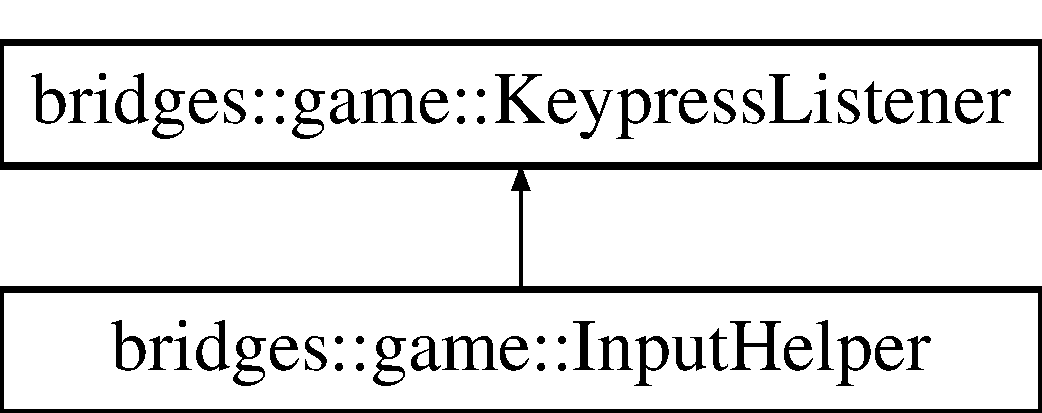
\includegraphics[height=2.000000cm]{classbridges_1_1game_1_1_input_helper}
\end{center}
\end{figure}


\doxysubsection{Detailed Description}
This is meant to be an internal class, not something that the library user will use. 

This class provide input device (mouse and keyboard) handling for \mbox{\hyperlink{classbridges_1_1_bridges}{Bridges}} games

\begin{DoxySeeAlso}{See also}
See the Games Tutorials at \href{https://bridgesuncc.github.io/tutorials/NonBlockingGame.html}{\texttt{ https\+://bridgesuncc.\+github.\+io/tutorials/\+Non\+Blocking\+Game.\+html}} for more information on keys and mouse device usage.
\end{DoxySeeAlso}
\begin{DoxyAuthor}{Author}
Erik Saule, David Burlinson 
\end{DoxyAuthor}
\begin{DoxyDate}{Date}
2018, 2019, 12/28/20 
\end{DoxyDate}
\doxysubsection*{Public Member Functions}
\begin{DoxyCompactItemize}
\item 
bool \mbox{\hyperlink{classbridges_1_1game_1_1_input_helper_aaa62faebd9e874228b710bb2a57cba2b}{key\+Up}} () const
\item 
bool \mbox{\hyperlink{classbridges_1_1game_1_1_input_helper_a904f5f5d2c6408bcd447044555cd376d}{key\+Down}} () const
\item 
bool \mbox{\hyperlink{classbridges_1_1game_1_1_input_helper_a9e98e137e69ef8b2f92e587092c42af4}{key\+Left}} () const
\item 
bool \mbox{\hyperlink{classbridges_1_1game_1_1_input_helper_a265fb9bd88d66e5439dd791bb90c79a4}{key\+Right}} () const
\item 
bool \mbox{\hyperlink{classbridges_1_1game_1_1_input_helper_a97a204c00019b28b4e95dde0b757a1aa}{keyW}} () const
\item 
bool \mbox{\hyperlink{classbridges_1_1game_1_1_input_helper_a168770e762b33e32597f9f7294082d9b}{keyA}} () const
\item 
bool \mbox{\hyperlink{classbridges_1_1game_1_1_input_helper_aa141b96b3406e66feab876185c7f350e}{keyS}} () const
\item 
bool \mbox{\hyperlink{classbridges_1_1game_1_1_input_helper_af7247d84254d706e3a309db2f4c20e9b}{keyD}} () const
\item 
bool \mbox{\hyperlink{classbridges_1_1game_1_1_input_helper_acef5fda1a5679e811fdf5a669dc65f9f}{keyQ}} () const
\item 
bool \mbox{\hyperlink{classbridges_1_1game_1_1_input_helper_a1750cd9c59e18126c251ec468fc87d48}{key\+Space}} () const
\end{DoxyCompactItemize}
\doxysubsection*{Protected Member Functions}
\begin{DoxyCompactItemize}
\item 
virtual void \mbox{\hyperlink{classbridges_1_1game_1_1_input_helper_aa847f19c6f68ebbb63d73802abfcd9a0}{keyup}} (std\+::string JSONmessage) override
\item 
virtual void \mbox{\hyperlink{classbridges_1_1game_1_1_input_helper_aac75c2b1abf28afa4acaf730e925f301}{keydown}} (std\+::string JSONmessage) override
\end{DoxyCompactItemize}


\doxysubsection{Member Function Documentation}
\mbox{\Hypertarget{classbridges_1_1game_1_1_input_helper_a168770e762b33e32597f9f7294082d9b}\label{classbridges_1_1game_1_1_input_helper_a168770e762b33e32597f9f7294082d9b}} 
\index{bridges::game::InputHelper@{bridges::game::InputHelper}!keyA@{keyA}}
\index{keyA@{keyA}!bridges::game::InputHelper@{bridges::game::InputHelper}}
\doxysubsubsection{\texorpdfstring{keyA()}{keyA()}}
{\footnotesize\ttfamily bool bridges\+::game\+::\+Input\+Helper\+::keyA (\begin{DoxyParamCaption}{ }\end{DoxyParamCaption}) const\hspace{0.3cm}{\ttfamily [inline]}}

\mbox{\Hypertarget{classbridges_1_1game_1_1_input_helper_af7247d84254d706e3a309db2f4c20e9b}\label{classbridges_1_1game_1_1_input_helper_af7247d84254d706e3a309db2f4c20e9b}} 
\index{bridges::game::InputHelper@{bridges::game::InputHelper}!keyD@{keyD}}
\index{keyD@{keyD}!bridges::game::InputHelper@{bridges::game::InputHelper}}
\doxysubsubsection{\texorpdfstring{keyD()}{keyD()}}
{\footnotesize\ttfamily bool bridges\+::game\+::\+Input\+Helper\+::keyD (\begin{DoxyParamCaption}{ }\end{DoxyParamCaption}) const\hspace{0.3cm}{\ttfamily [inline]}}

\mbox{\Hypertarget{classbridges_1_1game_1_1_input_helper_a904f5f5d2c6408bcd447044555cd376d}\label{classbridges_1_1game_1_1_input_helper_a904f5f5d2c6408bcd447044555cd376d}} 
\index{bridges::game::InputHelper@{bridges::game::InputHelper}!keyDown@{keyDown}}
\index{keyDown@{keyDown}!bridges::game::InputHelper@{bridges::game::InputHelper}}
\doxysubsubsection{\texorpdfstring{keyDown()}{keyDown()}}
{\footnotesize\ttfamily bool bridges\+::game\+::\+Input\+Helper\+::key\+Down (\begin{DoxyParamCaption}{ }\end{DoxyParamCaption}) const\hspace{0.3cm}{\ttfamily [inline]}}

\mbox{\Hypertarget{classbridges_1_1game_1_1_input_helper_aac75c2b1abf28afa4acaf730e925f301}\label{classbridges_1_1game_1_1_input_helper_aac75c2b1abf28afa4acaf730e925f301}} 
\index{bridges::game::InputHelper@{bridges::game::InputHelper}!keydown@{keydown}}
\index{keydown@{keydown}!bridges::game::InputHelper@{bridges::game::InputHelper}}
\doxysubsubsection{\texorpdfstring{keydown()}{keydown()}}
{\footnotesize\ttfamily virtual void bridges\+::game\+::\+Input\+Helper\+::keydown (\begin{DoxyParamCaption}\item[{std\+::string}]{JSONmessage }\end{DoxyParamCaption})\hspace{0.3cm}{\ttfamily [inline]}, {\ttfamily [override]}, {\ttfamily [protected]}, {\ttfamily [virtual]}}



Implements \mbox{\hyperlink{classbridges_1_1game_1_1_keypress_listener_a79362f390cad37bfe73012a05599e8aa}{bridges\+::game\+::\+Keypress\+Listener}}.

\mbox{\Hypertarget{classbridges_1_1game_1_1_input_helper_a9e98e137e69ef8b2f92e587092c42af4}\label{classbridges_1_1game_1_1_input_helper_a9e98e137e69ef8b2f92e587092c42af4}} 
\index{bridges::game::InputHelper@{bridges::game::InputHelper}!keyLeft@{keyLeft}}
\index{keyLeft@{keyLeft}!bridges::game::InputHelper@{bridges::game::InputHelper}}
\doxysubsubsection{\texorpdfstring{keyLeft()}{keyLeft()}}
{\footnotesize\ttfamily bool bridges\+::game\+::\+Input\+Helper\+::key\+Left (\begin{DoxyParamCaption}{ }\end{DoxyParamCaption}) const\hspace{0.3cm}{\ttfamily [inline]}}

\mbox{\Hypertarget{classbridges_1_1game_1_1_input_helper_acef5fda1a5679e811fdf5a669dc65f9f}\label{classbridges_1_1game_1_1_input_helper_acef5fda1a5679e811fdf5a669dc65f9f}} 
\index{bridges::game::InputHelper@{bridges::game::InputHelper}!keyQ@{keyQ}}
\index{keyQ@{keyQ}!bridges::game::InputHelper@{bridges::game::InputHelper}}
\doxysubsubsection{\texorpdfstring{keyQ()}{keyQ()}}
{\footnotesize\ttfamily bool bridges\+::game\+::\+Input\+Helper\+::keyQ (\begin{DoxyParamCaption}{ }\end{DoxyParamCaption}) const\hspace{0.3cm}{\ttfamily [inline]}}

\mbox{\Hypertarget{classbridges_1_1game_1_1_input_helper_a265fb9bd88d66e5439dd791bb90c79a4}\label{classbridges_1_1game_1_1_input_helper_a265fb9bd88d66e5439dd791bb90c79a4}} 
\index{bridges::game::InputHelper@{bridges::game::InputHelper}!keyRight@{keyRight}}
\index{keyRight@{keyRight}!bridges::game::InputHelper@{bridges::game::InputHelper}}
\doxysubsubsection{\texorpdfstring{keyRight()}{keyRight()}}
{\footnotesize\ttfamily bool bridges\+::game\+::\+Input\+Helper\+::key\+Right (\begin{DoxyParamCaption}{ }\end{DoxyParamCaption}) const\hspace{0.3cm}{\ttfamily [inline]}}

\mbox{\Hypertarget{classbridges_1_1game_1_1_input_helper_aa141b96b3406e66feab876185c7f350e}\label{classbridges_1_1game_1_1_input_helper_aa141b96b3406e66feab876185c7f350e}} 
\index{bridges::game::InputHelper@{bridges::game::InputHelper}!keyS@{keyS}}
\index{keyS@{keyS}!bridges::game::InputHelper@{bridges::game::InputHelper}}
\doxysubsubsection{\texorpdfstring{keyS()}{keyS()}}
{\footnotesize\ttfamily bool bridges\+::game\+::\+Input\+Helper\+::keyS (\begin{DoxyParamCaption}{ }\end{DoxyParamCaption}) const\hspace{0.3cm}{\ttfamily [inline]}}

\mbox{\Hypertarget{classbridges_1_1game_1_1_input_helper_a1750cd9c59e18126c251ec468fc87d48}\label{classbridges_1_1game_1_1_input_helper_a1750cd9c59e18126c251ec468fc87d48}} 
\index{bridges::game::InputHelper@{bridges::game::InputHelper}!keySpace@{keySpace}}
\index{keySpace@{keySpace}!bridges::game::InputHelper@{bridges::game::InputHelper}}
\doxysubsubsection{\texorpdfstring{keySpace()}{keySpace()}}
{\footnotesize\ttfamily bool bridges\+::game\+::\+Input\+Helper\+::key\+Space (\begin{DoxyParamCaption}{ }\end{DoxyParamCaption}) const\hspace{0.3cm}{\ttfamily [inline]}}

\mbox{\Hypertarget{classbridges_1_1game_1_1_input_helper_aaa62faebd9e874228b710bb2a57cba2b}\label{classbridges_1_1game_1_1_input_helper_aaa62faebd9e874228b710bb2a57cba2b}} 
\index{bridges::game::InputHelper@{bridges::game::InputHelper}!keyUp@{keyUp}}
\index{keyUp@{keyUp}!bridges::game::InputHelper@{bridges::game::InputHelper}}
\doxysubsubsection{\texorpdfstring{keyUp()}{keyUp()}}
{\footnotesize\ttfamily bool bridges\+::game\+::\+Input\+Helper\+::key\+Up (\begin{DoxyParamCaption}{ }\end{DoxyParamCaption}) const\hspace{0.3cm}{\ttfamily [inline]}}

\mbox{\Hypertarget{classbridges_1_1game_1_1_input_helper_aa847f19c6f68ebbb63d73802abfcd9a0}\label{classbridges_1_1game_1_1_input_helper_aa847f19c6f68ebbb63d73802abfcd9a0}} 
\index{bridges::game::InputHelper@{bridges::game::InputHelper}!keyup@{keyup}}
\index{keyup@{keyup}!bridges::game::InputHelper@{bridges::game::InputHelper}}
\doxysubsubsection{\texorpdfstring{keyup()}{keyup()}}
{\footnotesize\ttfamily virtual void bridges\+::game\+::\+Input\+Helper\+::keyup (\begin{DoxyParamCaption}\item[{std\+::string}]{JSONmessage }\end{DoxyParamCaption})\hspace{0.3cm}{\ttfamily [inline]}, {\ttfamily [override]}, {\ttfamily [protected]}, {\ttfamily [virtual]}}



Implements \mbox{\hyperlink{classbridges_1_1game_1_1_keypress_listener_a21d9f085819e30c41f3964ea2276964d}{bridges\+::game\+::\+Keypress\+Listener}}.

\mbox{\Hypertarget{classbridges_1_1game_1_1_input_helper_a97a204c00019b28b4e95dde0b757a1aa}\label{classbridges_1_1game_1_1_input_helper_a97a204c00019b28b4e95dde0b757a1aa}} 
\index{bridges::game::InputHelper@{bridges::game::InputHelper}!keyW@{keyW}}
\index{keyW@{keyW}!bridges::game::InputHelper@{bridges::game::InputHelper}}
\doxysubsubsection{\texorpdfstring{keyW()}{keyW()}}
{\footnotesize\ttfamily bool bridges\+::game\+::\+Input\+Helper\+::keyW (\begin{DoxyParamCaption}{ }\end{DoxyParamCaption}) const\hspace{0.3cm}{\ttfamily [inline]}}



The documentation for this class was generated from the following file\+:\begin{DoxyCompactItemize}
\item 
/home/erik/work/bridges/bridges-\/cxx/src/\mbox{\hyperlink{_input_helper_8h}{Input\+Helper.\+h}}\end{DoxyCompactItemize}

\hypertarget{classsio_1_1int__message}{}\doxysection{sio\+::int\+\_\+message Class Reference}
\label{classsio_1_1int__message}\index{sio::int\_message@{sio::int\_message}}


{\ttfamily \#include $<$sio\+\_\+message.\+h$>$}

Inheritance diagram for sio\+::int\+\_\+message\+:\begin{figure}[H]
\begin{center}
\leavevmode
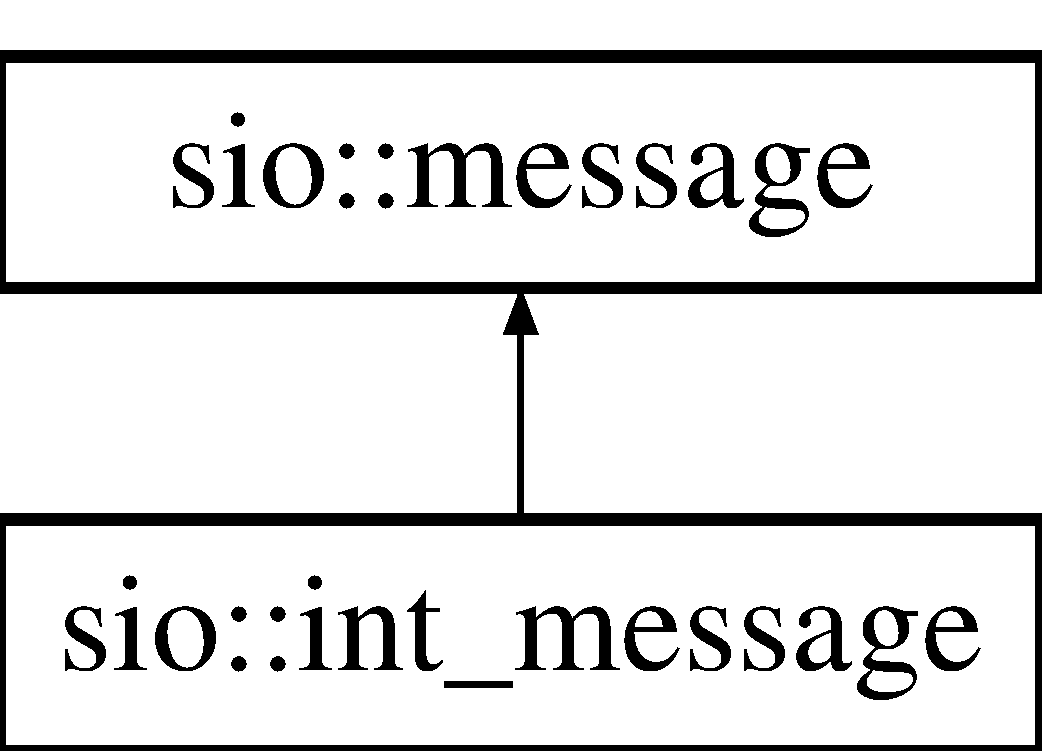
\includegraphics[height=2.000000cm]{classsio_1_1int__message}
\end{center}
\end{figure}
\doxysubsection*{Public Member Functions}
\begin{DoxyCompactItemize}
\item 
int64\+\_\+t \mbox{\hyperlink{classsio_1_1int__message_ad9159e1285bd3efd15b8f87699a9b133}{get\+\_\+int}} () const
\item 
double \mbox{\hyperlink{classsio_1_1int__message_a7fdc141b0fe04ce1b75054b6de110f2c}{get\+\_\+double}} () const
\end{DoxyCompactItemize}
\doxysubsection*{Static Public Member Functions}
\begin{DoxyCompactItemize}
\item 
static \mbox{\hyperlink{classsio_1_1message_a6340b6fef57e4516eb17928b1885a615}{message\+::ptr}} \mbox{\hyperlink{classsio_1_1int__message_afdff250333f3bd5253465ca6dbc86c61}{create}} (int64\+\_\+t v)
\end{DoxyCompactItemize}
\doxysubsection*{Protected Member Functions}
\begin{DoxyCompactItemize}
\item 
\mbox{\hyperlink{classsio_1_1int__message_a9d2da2260ddfdc421b5e0fb86a389a87}{int\+\_\+message}} (int64\+\_\+t v)
\end{DoxyCompactItemize}
\doxysubsection*{Additional Inherited Members}


\doxysubsection{Constructor \& Destructor Documentation}
\mbox{\Hypertarget{classsio_1_1int__message_a9d2da2260ddfdc421b5e0fb86a389a87}\label{classsio_1_1int__message_a9d2da2260ddfdc421b5e0fb86a389a87}} 
\index{sio::int\_message@{sio::int\_message}!int\_message@{int\_message}}
\index{int\_message@{int\_message}!sio::int\_message@{sio::int\_message}}
\doxysubsubsection{\texorpdfstring{int\_message()}{int\_message()}}
{\footnotesize\ttfamily sio\+::int\+\_\+message\+::int\+\_\+message (\begin{DoxyParamCaption}\item[{int64\+\_\+t}]{v }\end{DoxyParamCaption})\hspace{0.3cm}{\ttfamily [inline]}, {\ttfamily [protected]}}



\doxysubsection{Member Function Documentation}
\mbox{\Hypertarget{classsio_1_1int__message_afdff250333f3bd5253465ca6dbc86c61}\label{classsio_1_1int__message_afdff250333f3bd5253465ca6dbc86c61}} 
\index{sio::int\_message@{sio::int\_message}!create@{create}}
\index{create@{create}!sio::int\_message@{sio::int\_message}}
\doxysubsubsection{\texorpdfstring{create()}{create()}}
{\footnotesize\ttfamily static \mbox{\hyperlink{classsio_1_1message_a6340b6fef57e4516eb17928b1885a615}{message\+::ptr}} sio\+::int\+\_\+message\+::create (\begin{DoxyParamCaption}\item[{int64\+\_\+t}]{v }\end{DoxyParamCaption})\hspace{0.3cm}{\ttfamily [inline]}, {\ttfamily [static]}}

\mbox{\Hypertarget{classsio_1_1int__message_a7fdc141b0fe04ce1b75054b6de110f2c}\label{classsio_1_1int__message_a7fdc141b0fe04ce1b75054b6de110f2c}} 
\index{sio::int\_message@{sio::int\_message}!get\_double@{get\_double}}
\index{get\_double@{get\_double}!sio::int\_message@{sio::int\_message}}
\doxysubsubsection{\texorpdfstring{get\_double()}{get\_double()}}
{\footnotesize\ttfamily double sio\+::int\+\_\+message\+::get\+\_\+double (\begin{DoxyParamCaption}{ }\end{DoxyParamCaption}) const\hspace{0.3cm}{\ttfamily [inline]}, {\ttfamily [virtual]}}



Reimplemented from \mbox{\hyperlink{classsio_1_1message_aa89963cd233b29653df1ce1943f9ea57}{sio\+::message}}.

\mbox{\Hypertarget{classsio_1_1int__message_ad9159e1285bd3efd15b8f87699a9b133}\label{classsio_1_1int__message_ad9159e1285bd3efd15b8f87699a9b133}} 
\index{sio::int\_message@{sio::int\_message}!get\_int@{get\_int}}
\index{get\_int@{get\_int}!sio::int\_message@{sio::int\_message}}
\doxysubsubsection{\texorpdfstring{get\_int()}{get\_int()}}
{\footnotesize\ttfamily int64\+\_\+t sio\+::int\+\_\+message\+::get\+\_\+int (\begin{DoxyParamCaption}{ }\end{DoxyParamCaption}) const\hspace{0.3cm}{\ttfamily [inline]}, {\ttfamily [virtual]}}



Reimplemented from \mbox{\hyperlink{classsio_1_1message_ae77c363200284d6741f0ac92f0e13ed2}{sio\+::message}}.



The documentation for this class was generated from the following file\+:\begin{DoxyCompactItemize}
\item 
/home/erik/work/bridges/bridges-\/cxx/src/\mbox{\hyperlink{sio__message_8h}{sio\+\_\+message.\+h}}\end{DoxyCompactItemize}

\hypertarget{classbridges_1_1datastructure_1_1_array1_d_1_1iterator}{}\doxysection{bridges\+::datastructure\+::Array1D$<$ E $>$\+::iterator Class Reference}
\label{classbridges_1_1datastructure_1_1_array1_d_1_1iterator}\index{bridges::datastructure::Array1D$<$ E $>$::iterator@{bridges::datastructure::Array1D$<$ E $>$::iterator}}


{\ttfamily \#include $<$Array1\+D.\+h$>$}



\doxysubsection{Detailed Description}
\subsubsection*{template$<$typename E$>$\newline
class bridges\+::datastructure\+::\+Array1\+D$<$ E $>$\+::iterator}

enabling range for loops \doxysubsection*{Public Member Functions}
\begin{DoxyCompactItemize}
\item 
\mbox{\hyperlink{classbridges_1_1datastructure_1_1_array1_d_1_1iterator_a5bfe7e8948825c5814a95b05551496e4}{iterator}} (\mbox{\hyperlink{classbridges_1_1datastructure_1_1_array1_d}{Array1D}}$<$ E $>$ \&a, int ind)
\item 
E const  \& \mbox{\hyperlink{classbridges_1_1datastructure_1_1_array1_d_1_1iterator_a847f7a113b05007499eac3dca011ba5d}{operator$\ast$}} () const
\item 
E \& \mbox{\hyperlink{classbridges_1_1datastructure_1_1_array1_d_1_1iterator_aa95730146a48c7d753334fdcfddfbd84}{operator$\ast$}} ()
\item 
\mbox{\hyperlink{classbridges_1_1datastructure_1_1_array1_d_1_1iterator}{iterator}} \& \mbox{\hyperlink{classbridges_1_1datastructure_1_1_array1_d_1_1iterator_a1d8394de4e75cf1dffd1465beba2f85a}{operator++}} ()
\item 
\mbox{\hyperlink{classbridges_1_1datastructure_1_1_array1_d_1_1iterator}{iterator}} \& \mbox{\hyperlink{classbridges_1_1datastructure_1_1_array1_d_1_1iterator_ae63ca794e437c96e713a5c51844766f9}{operator-\/-\/}} ()
\item 
\mbox{\hyperlink{classbridges_1_1datastructure_1_1_array1_d_1_1iterator}{iterator}} \& \mbox{\hyperlink{classbridges_1_1datastructure_1_1_array1_d_1_1iterator_a113e2d57db9888db18681558b6ddd4c2}{operator++}} (int)
\item 
\mbox{\hyperlink{classbridges_1_1datastructure_1_1_array1_d_1_1iterator}{iterator}} \& \mbox{\hyperlink{classbridges_1_1datastructure_1_1_array1_d_1_1iterator_a600898496da4155d0c58399cf9d1b4cf}{operator-\/-\/}} (int)
\item 
bool \mbox{\hyperlink{classbridges_1_1datastructure_1_1_array1_d_1_1iterator_a59e1cdad748d872e7d07a26009a5a596}{operator==}} (const \mbox{\hyperlink{classbridges_1_1datastructure_1_1_array1_d_1_1iterator}{iterator}} \&it) const
\item 
bool \mbox{\hyperlink{classbridges_1_1datastructure_1_1_array1_d_1_1iterator_ab9e885078d2bb6068efa5ef899b7e32b}{operator!=}} (const \mbox{\hyperlink{classbridges_1_1datastructure_1_1_array1_d_1_1iterator}{iterator}} \&it) const
\end{DoxyCompactItemize}


\doxysubsection{Constructor \& Destructor Documentation}
\mbox{\Hypertarget{classbridges_1_1datastructure_1_1_array1_d_1_1iterator_a5bfe7e8948825c5814a95b05551496e4}\label{classbridges_1_1datastructure_1_1_array1_d_1_1iterator_a5bfe7e8948825c5814a95b05551496e4}} 
\index{bridges::datastructure::Array1D$<$ E $>$::iterator@{bridges::datastructure::Array1D$<$ E $>$::iterator}!iterator@{iterator}}
\index{iterator@{iterator}!bridges::datastructure::Array1D$<$ E $>$::iterator@{bridges::datastructure::Array1D$<$ E $>$::iterator}}
\doxysubsubsection{\texorpdfstring{iterator()}{iterator()}}
{\footnotesize\ttfamily template$<$typename E $>$ \\
\mbox{\hyperlink{classbridges_1_1datastructure_1_1_array1_d}{bridges\+::datastructure\+::\+Array1D}}$<$ E $>$\+::iterator\+::iterator (\begin{DoxyParamCaption}\item[{\mbox{\hyperlink{classbridges_1_1datastructure_1_1_array1_d}{Array1D}}$<$ E $>$ \&}]{a,  }\item[{int}]{ind }\end{DoxyParamCaption})\hspace{0.3cm}{\ttfamily [inline]}}



\doxysubsection{Member Function Documentation}
\mbox{\Hypertarget{classbridges_1_1datastructure_1_1_array1_d_1_1iterator_ab9e885078d2bb6068efa5ef899b7e32b}\label{classbridges_1_1datastructure_1_1_array1_d_1_1iterator_ab9e885078d2bb6068efa5ef899b7e32b}} 
\index{bridges::datastructure::Array1D$<$ E $>$::iterator@{bridges::datastructure::Array1D$<$ E $>$::iterator}!operator"!=@{operator"!=}}
\index{operator"!=@{operator"!=}!bridges::datastructure::Array1D$<$ E $>$::iterator@{bridges::datastructure::Array1D$<$ E $>$::iterator}}
\doxysubsubsection{\texorpdfstring{operator"!=()}{operator!=()}}
{\footnotesize\ttfamily template$<$typename E $>$ \\
bool \mbox{\hyperlink{classbridges_1_1datastructure_1_1_array1_d}{bridges\+::datastructure\+::\+Array1D}}$<$ E $>$\+::iterator\+::operator!= (\begin{DoxyParamCaption}\item[{const \mbox{\hyperlink{classbridges_1_1datastructure_1_1_array1_d_1_1iterator}{iterator}} \&}]{it }\end{DoxyParamCaption}) const\hspace{0.3cm}{\ttfamily [inline]}}

\mbox{\Hypertarget{classbridges_1_1datastructure_1_1_array1_d_1_1iterator_aa95730146a48c7d753334fdcfddfbd84}\label{classbridges_1_1datastructure_1_1_array1_d_1_1iterator_aa95730146a48c7d753334fdcfddfbd84}} 
\index{bridges::datastructure::Array1D$<$ E $>$::iterator@{bridges::datastructure::Array1D$<$ E $>$::iterator}!operator$\ast$@{operator$\ast$}}
\index{operator$\ast$@{operator$\ast$}!bridges::datastructure::Array1D$<$ E $>$::iterator@{bridges::datastructure::Array1D$<$ E $>$::iterator}}
\doxysubsubsection{\texorpdfstring{operator$\ast$()}{operator*()}\hspace{0.1cm}{\footnotesize\ttfamily [1/2]}}
{\footnotesize\ttfamily template$<$typename E $>$ \\
E\& \mbox{\hyperlink{classbridges_1_1datastructure_1_1_array1_d}{bridges\+::datastructure\+::\+Array1D}}$<$ E $>$\+::iterator\+::operator$\ast$ (\begin{DoxyParamCaption}{ }\end{DoxyParamCaption})\hspace{0.3cm}{\ttfamily [inline]}}

\mbox{\Hypertarget{classbridges_1_1datastructure_1_1_array1_d_1_1iterator_a847f7a113b05007499eac3dca011ba5d}\label{classbridges_1_1datastructure_1_1_array1_d_1_1iterator_a847f7a113b05007499eac3dca011ba5d}} 
\index{bridges::datastructure::Array1D$<$ E $>$::iterator@{bridges::datastructure::Array1D$<$ E $>$::iterator}!operator$\ast$@{operator$\ast$}}
\index{operator$\ast$@{operator$\ast$}!bridges::datastructure::Array1D$<$ E $>$::iterator@{bridges::datastructure::Array1D$<$ E $>$::iterator}}
\doxysubsubsection{\texorpdfstring{operator$\ast$()}{operator*()}\hspace{0.1cm}{\footnotesize\ttfamily [2/2]}}
{\footnotesize\ttfamily template$<$typename E $>$ \\
E const\& \mbox{\hyperlink{classbridges_1_1datastructure_1_1_array1_d}{bridges\+::datastructure\+::\+Array1D}}$<$ E $>$\+::iterator\+::operator$\ast$ (\begin{DoxyParamCaption}{ }\end{DoxyParamCaption}) const\hspace{0.3cm}{\ttfamily [inline]}}

\mbox{\Hypertarget{classbridges_1_1datastructure_1_1_array1_d_1_1iterator_a1d8394de4e75cf1dffd1465beba2f85a}\label{classbridges_1_1datastructure_1_1_array1_d_1_1iterator_a1d8394de4e75cf1dffd1465beba2f85a}} 
\index{bridges::datastructure::Array1D$<$ E $>$::iterator@{bridges::datastructure::Array1D$<$ E $>$::iterator}!operator++@{operator++}}
\index{operator++@{operator++}!bridges::datastructure::Array1D$<$ E $>$::iterator@{bridges::datastructure::Array1D$<$ E $>$::iterator}}
\doxysubsubsection{\texorpdfstring{operator++()}{operator++()}\hspace{0.1cm}{\footnotesize\ttfamily [1/2]}}
{\footnotesize\ttfamily template$<$typename E $>$ \\
\mbox{\hyperlink{classbridges_1_1datastructure_1_1_array1_d_1_1iterator}{iterator}}\& \mbox{\hyperlink{classbridges_1_1datastructure_1_1_array1_d}{bridges\+::datastructure\+::\+Array1D}}$<$ E $>$\+::iterator\+::operator++ (\begin{DoxyParamCaption}{ }\end{DoxyParamCaption})\hspace{0.3cm}{\ttfamily [inline]}}

\mbox{\Hypertarget{classbridges_1_1datastructure_1_1_array1_d_1_1iterator_a113e2d57db9888db18681558b6ddd4c2}\label{classbridges_1_1datastructure_1_1_array1_d_1_1iterator_a113e2d57db9888db18681558b6ddd4c2}} 
\index{bridges::datastructure::Array1D$<$ E $>$::iterator@{bridges::datastructure::Array1D$<$ E $>$::iterator}!operator++@{operator++}}
\index{operator++@{operator++}!bridges::datastructure::Array1D$<$ E $>$::iterator@{bridges::datastructure::Array1D$<$ E $>$::iterator}}
\doxysubsubsection{\texorpdfstring{operator++()}{operator++()}\hspace{0.1cm}{\footnotesize\ttfamily [2/2]}}
{\footnotesize\ttfamily template$<$typename E $>$ \\
\mbox{\hyperlink{classbridges_1_1datastructure_1_1_array1_d_1_1iterator}{iterator}}\& \mbox{\hyperlink{classbridges_1_1datastructure_1_1_array1_d}{bridges\+::datastructure\+::\+Array1D}}$<$ E $>$\+::iterator\+::operator++ (\begin{DoxyParamCaption}\item[{int}]{ }\end{DoxyParamCaption})\hspace{0.3cm}{\ttfamily [inline]}}

\mbox{\Hypertarget{classbridges_1_1datastructure_1_1_array1_d_1_1iterator_ae63ca794e437c96e713a5c51844766f9}\label{classbridges_1_1datastructure_1_1_array1_d_1_1iterator_ae63ca794e437c96e713a5c51844766f9}} 
\index{bridges::datastructure::Array1D$<$ E $>$::iterator@{bridges::datastructure::Array1D$<$ E $>$::iterator}!operator-\/-\/@{operator-\/-\/}}
\index{operator-\/-\/@{operator-\/-\/}!bridges::datastructure::Array1D$<$ E $>$::iterator@{bridges::datastructure::Array1D$<$ E $>$::iterator}}
\doxysubsubsection{\texorpdfstring{operator-\/-\/()}{operator--()}\hspace{0.1cm}{\footnotesize\ttfamily [1/2]}}
{\footnotesize\ttfamily template$<$typename E $>$ \\
\mbox{\hyperlink{classbridges_1_1datastructure_1_1_array1_d_1_1iterator}{iterator}}\& \mbox{\hyperlink{classbridges_1_1datastructure_1_1_array1_d}{bridges\+::datastructure\+::\+Array1D}}$<$ E $>$\+::iterator\+::operator-\/-\/ (\begin{DoxyParamCaption}{ }\end{DoxyParamCaption})\hspace{0.3cm}{\ttfamily [inline]}}

\mbox{\Hypertarget{classbridges_1_1datastructure_1_1_array1_d_1_1iterator_a600898496da4155d0c58399cf9d1b4cf}\label{classbridges_1_1datastructure_1_1_array1_d_1_1iterator_a600898496da4155d0c58399cf9d1b4cf}} 
\index{bridges::datastructure::Array1D$<$ E $>$::iterator@{bridges::datastructure::Array1D$<$ E $>$::iterator}!operator-\/-\/@{operator-\/-\/}}
\index{operator-\/-\/@{operator-\/-\/}!bridges::datastructure::Array1D$<$ E $>$::iterator@{bridges::datastructure::Array1D$<$ E $>$::iterator}}
\doxysubsubsection{\texorpdfstring{operator-\/-\/()}{operator--()}\hspace{0.1cm}{\footnotesize\ttfamily [2/2]}}
{\footnotesize\ttfamily template$<$typename E $>$ \\
\mbox{\hyperlink{classbridges_1_1datastructure_1_1_array1_d_1_1iterator}{iterator}}\& \mbox{\hyperlink{classbridges_1_1datastructure_1_1_array1_d}{bridges\+::datastructure\+::\+Array1D}}$<$ E $>$\+::iterator\+::operator-\/-\/ (\begin{DoxyParamCaption}\item[{int}]{ }\end{DoxyParamCaption})\hspace{0.3cm}{\ttfamily [inline]}}

\mbox{\Hypertarget{classbridges_1_1datastructure_1_1_array1_d_1_1iterator_a59e1cdad748d872e7d07a26009a5a596}\label{classbridges_1_1datastructure_1_1_array1_d_1_1iterator_a59e1cdad748d872e7d07a26009a5a596}} 
\index{bridges::datastructure::Array1D$<$ E $>$::iterator@{bridges::datastructure::Array1D$<$ E $>$::iterator}!operator==@{operator==}}
\index{operator==@{operator==}!bridges::datastructure::Array1D$<$ E $>$::iterator@{bridges::datastructure::Array1D$<$ E $>$::iterator}}
\doxysubsubsection{\texorpdfstring{operator==()}{operator==()}}
{\footnotesize\ttfamily template$<$typename E $>$ \\
bool \mbox{\hyperlink{classbridges_1_1datastructure_1_1_array1_d}{bridges\+::datastructure\+::\+Array1D}}$<$ E $>$\+::iterator\+::operator== (\begin{DoxyParamCaption}\item[{const \mbox{\hyperlink{classbridges_1_1datastructure_1_1_array1_d_1_1iterator}{iterator}} \&}]{it }\end{DoxyParamCaption}) const\hspace{0.3cm}{\ttfamily [inline]}}



The documentation for this class was generated from the following file\+:\begin{DoxyCompactItemize}
\item 
/home/erik/work/bridges/bridges-\/cxx/src/\mbox{\hyperlink{_array1_d_8h}{Array1\+D.\+h}}\end{DoxyCompactItemize}

\hypertarget{classbridges_1_1datastructure_1_1_s_lelement_1_1_s_lelement__constlisthelper_1_1iterator}{}\section{bridges\+:\+:datastructure\+:\+:S\+Lelement$<$ E $>$\+:\+:S\+Lelement\+\_\+constlisthelper\+:\+:iterator Class Reference}
\label{classbridges_1_1datastructure_1_1_s_lelement_1_1_s_lelement__constlisthelper_1_1iterator}\index{bridges\+::datastructure\+::\+S\+Lelement$<$ E $>$\+::\+S\+Lelement\+\_\+constlisthelper\+::iterator@{bridges\+::datastructure\+::\+S\+Lelement$<$ E $>$\+::\+S\+Lelement\+\_\+constlisthelper\+::iterator}}


{\ttfamily \#include $<$S\+Lelement.\+h$>$}

\subsection*{Public Member Functions}
\begin{DoxyCompactItemize}
\item 
\mbox{\hyperlink{classbridges_1_1datastructure_1_1_s_lelement_1_1_s_lelement__constlisthelper_1_1iterator_a438b2bda67331a3a989ea5fa45c30f7f}{iterator}} (typename \mbox{\hyperlink{classbridges_1_1datastructure_1_1_s_lelement}{bridges\+::datastructure\+::\+S\+Lelement}}$<$ E $>$ const $\ast$c)
\item 
bool \mbox{\hyperlink{classbridges_1_1datastructure_1_1_s_lelement_1_1_s_lelement__constlisthelper_1_1iterator_a65e17e54ef5f08c3deaee084951bda6a}{operator!=}} (const \mbox{\hyperlink{classbridges_1_1datastructure_1_1_s_lelement_1_1_s_lelement__constlisthelper_1_1iterator}{iterator}} \&it) const
\item 
E const  \& \mbox{\hyperlink{classbridges_1_1datastructure_1_1_s_lelement_1_1_s_lelement__constlisthelper_1_1iterator_a8d41bb42239d7df41879aa67d15842ed}{operator$\ast$}} () const
\item 
\mbox{\hyperlink{classbridges_1_1datastructure_1_1_s_lelement_1_1_s_lelement__constlisthelper_1_1iterator}{iterator}} \& \mbox{\hyperlink{classbridges_1_1datastructure_1_1_s_lelement_1_1_s_lelement__constlisthelper_1_1iterator_a3ae6ebe78df57195446770f1c7872fdd}{operator++}} ()
\end{DoxyCompactItemize}


\subsection{Constructor \& Destructor Documentation}
\mbox{\Hypertarget{classbridges_1_1datastructure_1_1_s_lelement_1_1_s_lelement__constlisthelper_1_1iterator_a438b2bda67331a3a989ea5fa45c30f7f}\label{classbridges_1_1datastructure_1_1_s_lelement_1_1_s_lelement__constlisthelper_1_1iterator_a438b2bda67331a3a989ea5fa45c30f7f}} 
\index{bridges\+::datastructure\+::\+S\+Lelement\+::\+S\+Lelement\+\_\+constlisthelper\+::iterator@{bridges\+::datastructure\+::\+S\+Lelement\+::\+S\+Lelement\+\_\+constlisthelper\+::iterator}!iterator@{iterator}}
\index{iterator@{iterator}!bridges\+::datastructure\+::\+S\+Lelement\+::\+S\+Lelement\+\_\+constlisthelper\+::iterator@{bridges\+::datastructure\+::\+S\+Lelement\+::\+S\+Lelement\+\_\+constlisthelper\+::iterator}}
\subsubsection{\texorpdfstring{iterator()}{iterator()}}
{\footnotesize\ttfamily template$<$typename E$>$ \\
\mbox{\hyperlink{classbridges_1_1datastructure_1_1_s_lelement}{bridges\+::datastructure\+::\+S\+Lelement}}$<$ E $>$\+::S\+Lelement\+\_\+constlisthelper\+::iterator\+::iterator (\begin{DoxyParamCaption}\item[{typename \mbox{\hyperlink{classbridges_1_1datastructure_1_1_s_lelement}{bridges\+::datastructure\+::\+S\+Lelement}}$<$ E $>$ const $\ast$}]{c }\end{DoxyParamCaption})\hspace{0.3cm}{\ttfamily [inline]}}



\subsection{Member Function Documentation}
\mbox{\Hypertarget{classbridges_1_1datastructure_1_1_s_lelement_1_1_s_lelement__constlisthelper_1_1iterator_a65e17e54ef5f08c3deaee084951bda6a}\label{classbridges_1_1datastructure_1_1_s_lelement_1_1_s_lelement__constlisthelper_1_1iterator_a65e17e54ef5f08c3deaee084951bda6a}} 
\index{bridges\+::datastructure\+::\+S\+Lelement\+::\+S\+Lelement\+\_\+constlisthelper\+::iterator@{bridges\+::datastructure\+::\+S\+Lelement\+::\+S\+Lelement\+\_\+constlisthelper\+::iterator}!operator"!=@{operator"!=}}
\index{operator"!=@{operator"!=}!bridges\+::datastructure\+::\+S\+Lelement\+::\+S\+Lelement\+\_\+constlisthelper\+::iterator@{bridges\+::datastructure\+::\+S\+Lelement\+::\+S\+Lelement\+\_\+constlisthelper\+::iterator}}
\subsubsection{\texorpdfstring{operator"!=()}{operator!=()}}
{\footnotesize\ttfamily template$<$typename E$>$ \\
bool \mbox{\hyperlink{classbridges_1_1datastructure_1_1_s_lelement}{bridges\+::datastructure\+::\+S\+Lelement}}$<$ E $>$\+::S\+Lelement\+\_\+constlisthelper\+::iterator\+::operator!= (\begin{DoxyParamCaption}\item[{const \mbox{\hyperlink{classbridges_1_1datastructure_1_1_s_lelement_1_1_s_lelement__constlisthelper_1_1iterator}{iterator}} \&}]{it }\end{DoxyParamCaption}) const\hspace{0.3cm}{\ttfamily [inline]}}

\mbox{\Hypertarget{classbridges_1_1datastructure_1_1_s_lelement_1_1_s_lelement__constlisthelper_1_1iterator_a8d41bb42239d7df41879aa67d15842ed}\label{classbridges_1_1datastructure_1_1_s_lelement_1_1_s_lelement__constlisthelper_1_1iterator_a8d41bb42239d7df41879aa67d15842ed}} 
\index{bridges\+::datastructure\+::\+S\+Lelement\+::\+S\+Lelement\+\_\+constlisthelper\+::iterator@{bridges\+::datastructure\+::\+S\+Lelement\+::\+S\+Lelement\+\_\+constlisthelper\+::iterator}!operator$\ast$@{operator$\ast$}}
\index{operator$\ast$@{operator$\ast$}!bridges\+::datastructure\+::\+S\+Lelement\+::\+S\+Lelement\+\_\+constlisthelper\+::iterator@{bridges\+::datastructure\+::\+S\+Lelement\+::\+S\+Lelement\+\_\+constlisthelper\+::iterator}}
\subsubsection{\texorpdfstring{operator$\ast$()}{operator*()}}
{\footnotesize\ttfamily template$<$typename E$>$ \\
E const\& \mbox{\hyperlink{classbridges_1_1datastructure_1_1_s_lelement}{bridges\+::datastructure\+::\+S\+Lelement}}$<$ E $>$\+::S\+Lelement\+\_\+constlisthelper\+::iterator\+::operator$\ast$ (\begin{DoxyParamCaption}{ }\end{DoxyParamCaption}) const\hspace{0.3cm}{\ttfamily [inline]}}

\mbox{\Hypertarget{classbridges_1_1datastructure_1_1_s_lelement_1_1_s_lelement__constlisthelper_1_1iterator_a3ae6ebe78df57195446770f1c7872fdd}\label{classbridges_1_1datastructure_1_1_s_lelement_1_1_s_lelement__constlisthelper_1_1iterator_a3ae6ebe78df57195446770f1c7872fdd}} 
\index{bridges\+::datastructure\+::\+S\+Lelement\+::\+S\+Lelement\+\_\+constlisthelper\+::iterator@{bridges\+::datastructure\+::\+S\+Lelement\+::\+S\+Lelement\+\_\+constlisthelper\+::iterator}!operator++@{operator++}}
\index{operator++@{operator++}!bridges\+::datastructure\+::\+S\+Lelement\+::\+S\+Lelement\+\_\+constlisthelper\+::iterator@{bridges\+::datastructure\+::\+S\+Lelement\+::\+S\+Lelement\+\_\+constlisthelper\+::iterator}}
\subsubsection{\texorpdfstring{operator++()}{operator++()}}
{\footnotesize\ttfamily template$<$typename E$>$ \\
\mbox{\hyperlink{classbridges_1_1datastructure_1_1_s_lelement_1_1_s_lelement__constlisthelper_1_1iterator}{iterator}}\& \mbox{\hyperlink{classbridges_1_1datastructure_1_1_s_lelement}{bridges\+::datastructure\+::\+S\+Lelement}}$<$ E $>$\+::S\+Lelement\+\_\+constlisthelper\+::iterator\+::operator++ (\begin{DoxyParamCaption}{ }\end{DoxyParamCaption})\hspace{0.3cm}{\ttfamily [inline]}}



The documentation for this class was generated from the following file\+:\begin{DoxyCompactItemize}
\item 
/\+Users/kalpathi/gr/bridges/client/cxx/src/\mbox{\hyperlink{_s_lelement_8h}{S\+Lelement.\+h}}\end{DoxyCompactItemize}

\hypertarget{classbridges_1_1datastructure_1_1_circ_d_lelement_1_1_circ_d_lelement__listhelper_1_1iterator}{}\doxysection{bridges\+::datastructure\+::Circ\+DLelement$<$ E $>$\+::Circ\+DLelement\+\_\+listhelper\+::iterator Class Reference}
\label{classbridges_1_1datastructure_1_1_circ_d_lelement_1_1_circ_d_lelement__listhelper_1_1iterator}\index{bridges::datastructure::CircDLelement$<$ E $>$::CircDLelement\_listhelper::iterator@{bridges::datastructure::CircDLelement$<$ E $>$::CircDLelement\_listhelper::iterator}}


{\ttfamily \#include $<$Circ\+DLelement.\+h$>$}

\doxysubsection*{Public Member Functions}
\begin{DoxyCompactItemize}
\item 
\mbox{\hyperlink{classbridges_1_1datastructure_1_1_circ_d_lelement_1_1_circ_d_lelement__listhelper_1_1iterator_af584c96d1a02d138a7db83815cee6428}{iterator}} (typename \mbox{\hyperlink{classbridges_1_1datastructure_1_1_circ_d_lelement}{bridges\+::datastructure\+::\+Circ\+DLelement}}$<$ E $>$ $\ast$c)
\item 
bool \mbox{\hyperlink{classbridges_1_1datastructure_1_1_circ_d_lelement_1_1_circ_d_lelement__listhelper_1_1iterator_a2739037e24a59ec4e8e69871451d43cf}{operator!=}} (const \mbox{\hyperlink{classbridges_1_1datastructure_1_1_circ_d_lelement_1_1_circ_d_lelement__listhelper_1_1iterator}{iterator}} \&it) const
\item 
E const  \& \mbox{\hyperlink{classbridges_1_1datastructure_1_1_circ_d_lelement_1_1_circ_d_lelement__listhelper_1_1iterator_a66bc18d767802d2dc172f5eb1ebb1a6e}{operator$\ast$}} () const
\item 
E \& \mbox{\hyperlink{classbridges_1_1datastructure_1_1_circ_d_lelement_1_1_circ_d_lelement__listhelper_1_1iterator_ad850d592029ecbb8e95c2e9e2fafe861}{operator$\ast$}} ()
\item 
\mbox{\hyperlink{classbridges_1_1datastructure_1_1_circ_d_lelement_1_1_circ_d_lelement__listhelper_1_1iterator}{iterator}} \& \mbox{\hyperlink{classbridges_1_1datastructure_1_1_circ_d_lelement_1_1_circ_d_lelement__listhelper_1_1iterator_aabfb538351c45de78af080249d014d47}{operator++}} ()
\item 
\mbox{\hyperlink{classbridges_1_1datastructure_1_1_circ_d_lelement_1_1_circ_d_lelement__listhelper_1_1iterator}{iterator}} \mbox{\hyperlink{classbridges_1_1datastructure_1_1_circ_d_lelement_1_1_circ_d_lelement__listhelper_1_1iterator_a02438c2e20111e85b053b2150f26bbf9}{operator++}} (int)
\item 
\mbox{\hyperlink{classbridges_1_1datastructure_1_1_circ_d_lelement_1_1_circ_d_lelement__listhelper_1_1iterator}{iterator}} \& \mbox{\hyperlink{classbridges_1_1datastructure_1_1_circ_d_lelement_1_1_circ_d_lelement__listhelper_1_1iterator_a88ebb96d0376f289b8520c33a77f1269}{operator-\/-\/}} ()
\item 
\mbox{\hyperlink{classbridges_1_1datastructure_1_1_circ_d_lelement_1_1_circ_d_lelement__listhelper_1_1iterator}{iterator}} \mbox{\hyperlink{classbridges_1_1datastructure_1_1_circ_d_lelement_1_1_circ_d_lelement__listhelper_1_1iterator_aa92dbdc5af7168113518f5c1d4eeb91c}{operator-\/-\/}} (int)
\end{DoxyCompactItemize}


\doxysubsection{Constructor \& Destructor Documentation}
\mbox{\Hypertarget{classbridges_1_1datastructure_1_1_circ_d_lelement_1_1_circ_d_lelement__listhelper_1_1iterator_af584c96d1a02d138a7db83815cee6428}\label{classbridges_1_1datastructure_1_1_circ_d_lelement_1_1_circ_d_lelement__listhelper_1_1iterator_af584c96d1a02d138a7db83815cee6428}} 
\index{bridges::datastructure::CircDLelement$<$ E $>$::CircDLelement\_listhelper::iterator@{bridges::datastructure::CircDLelement$<$ E $>$::CircDLelement\_listhelper::iterator}!iterator@{iterator}}
\index{iterator@{iterator}!bridges::datastructure::CircDLelement$<$ E $>$::CircDLelement\_listhelper::iterator@{bridges::datastructure::CircDLelement$<$ E $>$::CircDLelement\_listhelper::iterator}}
\doxysubsubsection{\texorpdfstring{iterator()}{iterator()}}
{\footnotesize\ttfamily template$<$typename E $>$ \\
\mbox{\hyperlink{classbridges_1_1datastructure_1_1_circ_d_lelement}{bridges\+::datastructure\+::\+Circ\+DLelement}}$<$ E $>$\+::Circ\+DLelement\+\_\+listhelper\+::iterator\+::iterator (\begin{DoxyParamCaption}\item[{typename \mbox{\hyperlink{classbridges_1_1datastructure_1_1_circ_d_lelement}{bridges\+::datastructure\+::\+Circ\+DLelement}}$<$ E $>$ $\ast$}]{c }\end{DoxyParamCaption})\hspace{0.3cm}{\ttfamily [inline]}}



\doxysubsection{Member Function Documentation}
\mbox{\Hypertarget{classbridges_1_1datastructure_1_1_circ_d_lelement_1_1_circ_d_lelement__listhelper_1_1iterator_a2739037e24a59ec4e8e69871451d43cf}\label{classbridges_1_1datastructure_1_1_circ_d_lelement_1_1_circ_d_lelement__listhelper_1_1iterator_a2739037e24a59ec4e8e69871451d43cf}} 
\index{bridges::datastructure::CircDLelement$<$ E $>$::CircDLelement\_listhelper::iterator@{bridges::datastructure::CircDLelement$<$ E $>$::CircDLelement\_listhelper::iterator}!operator"!=@{operator"!=}}
\index{operator"!=@{operator"!=}!bridges::datastructure::CircDLelement$<$ E $>$::CircDLelement\_listhelper::iterator@{bridges::datastructure::CircDLelement$<$ E $>$::CircDLelement\_listhelper::iterator}}
\doxysubsubsection{\texorpdfstring{operator"!=()}{operator!=()}}
{\footnotesize\ttfamily template$<$typename E $>$ \\
bool \mbox{\hyperlink{classbridges_1_1datastructure_1_1_circ_d_lelement}{bridges\+::datastructure\+::\+Circ\+DLelement}}$<$ E $>$\+::Circ\+DLelement\+\_\+listhelper\+::iterator\+::operator!= (\begin{DoxyParamCaption}\item[{const \mbox{\hyperlink{classbridges_1_1datastructure_1_1_circ_d_lelement_1_1_circ_d_lelement__listhelper_1_1iterator}{iterator}} \&}]{it }\end{DoxyParamCaption}) const\hspace{0.3cm}{\ttfamily [inline]}}

\mbox{\Hypertarget{classbridges_1_1datastructure_1_1_circ_d_lelement_1_1_circ_d_lelement__listhelper_1_1iterator_ad850d592029ecbb8e95c2e9e2fafe861}\label{classbridges_1_1datastructure_1_1_circ_d_lelement_1_1_circ_d_lelement__listhelper_1_1iterator_ad850d592029ecbb8e95c2e9e2fafe861}} 
\index{bridges::datastructure::CircDLelement$<$ E $>$::CircDLelement\_listhelper::iterator@{bridges::datastructure::CircDLelement$<$ E $>$::CircDLelement\_listhelper::iterator}!operator$\ast$@{operator$\ast$}}
\index{operator$\ast$@{operator$\ast$}!bridges::datastructure::CircDLelement$<$ E $>$::CircDLelement\_listhelper::iterator@{bridges::datastructure::CircDLelement$<$ E $>$::CircDLelement\_listhelper::iterator}}
\doxysubsubsection{\texorpdfstring{operator$\ast$()}{operator*()}\hspace{0.1cm}{\footnotesize\ttfamily [1/2]}}
{\footnotesize\ttfamily template$<$typename E $>$ \\
E\& \mbox{\hyperlink{classbridges_1_1datastructure_1_1_circ_d_lelement}{bridges\+::datastructure\+::\+Circ\+DLelement}}$<$ E $>$\+::Circ\+DLelement\+\_\+listhelper\+::iterator\+::operator$\ast$ (\begin{DoxyParamCaption}{ }\end{DoxyParamCaption})\hspace{0.3cm}{\ttfamily [inline]}}

\mbox{\Hypertarget{classbridges_1_1datastructure_1_1_circ_d_lelement_1_1_circ_d_lelement__listhelper_1_1iterator_a66bc18d767802d2dc172f5eb1ebb1a6e}\label{classbridges_1_1datastructure_1_1_circ_d_lelement_1_1_circ_d_lelement__listhelper_1_1iterator_a66bc18d767802d2dc172f5eb1ebb1a6e}} 
\index{bridges::datastructure::CircDLelement$<$ E $>$::CircDLelement\_listhelper::iterator@{bridges::datastructure::CircDLelement$<$ E $>$::CircDLelement\_listhelper::iterator}!operator$\ast$@{operator$\ast$}}
\index{operator$\ast$@{operator$\ast$}!bridges::datastructure::CircDLelement$<$ E $>$::CircDLelement\_listhelper::iterator@{bridges::datastructure::CircDLelement$<$ E $>$::CircDLelement\_listhelper::iterator}}
\doxysubsubsection{\texorpdfstring{operator$\ast$()}{operator*()}\hspace{0.1cm}{\footnotesize\ttfamily [2/2]}}
{\footnotesize\ttfamily template$<$typename E $>$ \\
E const\& \mbox{\hyperlink{classbridges_1_1datastructure_1_1_circ_d_lelement}{bridges\+::datastructure\+::\+Circ\+DLelement}}$<$ E $>$\+::Circ\+DLelement\+\_\+listhelper\+::iterator\+::operator$\ast$ (\begin{DoxyParamCaption}{ }\end{DoxyParamCaption}) const\hspace{0.3cm}{\ttfamily [inline]}}

\mbox{\Hypertarget{classbridges_1_1datastructure_1_1_circ_d_lelement_1_1_circ_d_lelement__listhelper_1_1iterator_aabfb538351c45de78af080249d014d47}\label{classbridges_1_1datastructure_1_1_circ_d_lelement_1_1_circ_d_lelement__listhelper_1_1iterator_aabfb538351c45de78af080249d014d47}} 
\index{bridges::datastructure::CircDLelement$<$ E $>$::CircDLelement\_listhelper::iterator@{bridges::datastructure::CircDLelement$<$ E $>$::CircDLelement\_listhelper::iterator}!operator++@{operator++}}
\index{operator++@{operator++}!bridges::datastructure::CircDLelement$<$ E $>$::CircDLelement\_listhelper::iterator@{bridges::datastructure::CircDLelement$<$ E $>$::CircDLelement\_listhelper::iterator}}
\doxysubsubsection{\texorpdfstring{operator++()}{operator++()}\hspace{0.1cm}{\footnotesize\ttfamily [1/2]}}
{\footnotesize\ttfamily template$<$typename E $>$ \\
\mbox{\hyperlink{classbridges_1_1datastructure_1_1_circ_d_lelement_1_1_circ_d_lelement__listhelper_1_1iterator}{iterator}}\& \mbox{\hyperlink{classbridges_1_1datastructure_1_1_circ_d_lelement}{bridges\+::datastructure\+::\+Circ\+DLelement}}$<$ E $>$\+::Circ\+DLelement\+\_\+listhelper\+::iterator\+::operator++ (\begin{DoxyParamCaption}{ }\end{DoxyParamCaption})\hspace{0.3cm}{\ttfamily [inline]}}

\mbox{\Hypertarget{classbridges_1_1datastructure_1_1_circ_d_lelement_1_1_circ_d_lelement__listhelper_1_1iterator_a02438c2e20111e85b053b2150f26bbf9}\label{classbridges_1_1datastructure_1_1_circ_d_lelement_1_1_circ_d_lelement__listhelper_1_1iterator_a02438c2e20111e85b053b2150f26bbf9}} 
\index{bridges::datastructure::CircDLelement$<$ E $>$::CircDLelement\_listhelper::iterator@{bridges::datastructure::CircDLelement$<$ E $>$::CircDLelement\_listhelper::iterator}!operator++@{operator++}}
\index{operator++@{operator++}!bridges::datastructure::CircDLelement$<$ E $>$::CircDLelement\_listhelper::iterator@{bridges::datastructure::CircDLelement$<$ E $>$::CircDLelement\_listhelper::iterator}}
\doxysubsubsection{\texorpdfstring{operator++()}{operator++()}\hspace{0.1cm}{\footnotesize\ttfamily [2/2]}}
{\footnotesize\ttfamily template$<$typename E $>$ \\
\mbox{\hyperlink{classbridges_1_1datastructure_1_1_circ_d_lelement_1_1_circ_d_lelement__listhelper_1_1iterator}{iterator}} \mbox{\hyperlink{classbridges_1_1datastructure_1_1_circ_d_lelement}{bridges\+::datastructure\+::\+Circ\+DLelement}}$<$ E $>$\+::Circ\+DLelement\+\_\+listhelper\+::iterator\+::operator++ (\begin{DoxyParamCaption}\item[{int}]{ }\end{DoxyParamCaption})\hspace{0.3cm}{\ttfamily [inline]}}

\mbox{\Hypertarget{classbridges_1_1datastructure_1_1_circ_d_lelement_1_1_circ_d_lelement__listhelper_1_1iterator_a88ebb96d0376f289b8520c33a77f1269}\label{classbridges_1_1datastructure_1_1_circ_d_lelement_1_1_circ_d_lelement__listhelper_1_1iterator_a88ebb96d0376f289b8520c33a77f1269}} 
\index{bridges::datastructure::CircDLelement$<$ E $>$::CircDLelement\_listhelper::iterator@{bridges::datastructure::CircDLelement$<$ E $>$::CircDLelement\_listhelper::iterator}!operator-\/-\/@{operator-\/-\/}}
\index{operator-\/-\/@{operator-\/-\/}!bridges::datastructure::CircDLelement$<$ E $>$::CircDLelement\_listhelper::iterator@{bridges::datastructure::CircDLelement$<$ E $>$::CircDLelement\_listhelper::iterator}}
\doxysubsubsection{\texorpdfstring{operator-\/-\/()}{operator--()}\hspace{0.1cm}{\footnotesize\ttfamily [1/2]}}
{\footnotesize\ttfamily template$<$typename E $>$ \\
\mbox{\hyperlink{classbridges_1_1datastructure_1_1_circ_d_lelement_1_1_circ_d_lelement__listhelper_1_1iterator}{iterator}}\& \mbox{\hyperlink{classbridges_1_1datastructure_1_1_circ_d_lelement}{bridges\+::datastructure\+::\+Circ\+DLelement}}$<$ E $>$\+::Circ\+DLelement\+\_\+listhelper\+::iterator\+::operator-\/-\/ (\begin{DoxyParamCaption}{ }\end{DoxyParamCaption})\hspace{0.3cm}{\ttfamily [inline]}}

\mbox{\Hypertarget{classbridges_1_1datastructure_1_1_circ_d_lelement_1_1_circ_d_lelement__listhelper_1_1iterator_aa92dbdc5af7168113518f5c1d4eeb91c}\label{classbridges_1_1datastructure_1_1_circ_d_lelement_1_1_circ_d_lelement__listhelper_1_1iterator_aa92dbdc5af7168113518f5c1d4eeb91c}} 
\index{bridges::datastructure::CircDLelement$<$ E $>$::CircDLelement\_listhelper::iterator@{bridges::datastructure::CircDLelement$<$ E $>$::CircDLelement\_listhelper::iterator}!operator-\/-\/@{operator-\/-\/}}
\index{operator-\/-\/@{operator-\/-\/}!bridges::datastructure::CircDLelement$<$ E $>$::CircDLelement\_listhelper::iterator@{bridges::datastructure::CircDLelement$<$ E $>$::CircDLelement\_listhelper::iterator}}
\doxysubsubsection{\texorpdfstring{operator-\/-\/()}{operator--()}\hspace{0.1cm}{\footnotesize\ttfamily [2/2]}}
{\footnotesize\ttfamily template$<$typename E $>$ \\
\mbox{\hyperlink{classbridges_1_1datastructure_1_1_circ_d_lelement_1_1_circ_d_lelement__listhelper_1_1iterator}{iterator}} \mbox{\hyperlink{classbridges_1_1datastructure_1_1_circ_d_lelement}{bridges\+::datastructure\+::\+Circ\+DLelement}}$<$ E $>$\+::Circ\+DLelement\+\_\+listhelper\+::iterator\+::operator-\/-\/ (\begin{DoxyParamCaption}\item[{int}]{ }\end{DoxyParamCaption})\hspace{0.3cm}{\ttfamily [inline]}}



The documentation for this class was generated from the following file\+:\begin{DoxyCompactItemize}
\item 
/home/erik/work/bridges/bridges-\/cxx/src/\mbox{\hyperlink{_circ_d_lelement_8h}{Circ\+DLelement.\+h}}\end{DoxyCompactItemize}

\hypertarget{classbridges_1_1datastructure_1_1_circ_d_lelement_1_1_circ_d_lelement__constlisthelper_1_1iterator}{}\doxysection{bridges\+::datastructure\+::Circ\+DLelement$<$ E $>$\+::Circ\+DLelement\+\_\+constlisthelper\+::iterator Class Reference}
\label{classbridges_1_1datastructure_1_1_circ_d_lelement_1_1_circ_d_lelement__constlisthelper_1_1iterator}\index{bridges::datastructure::CircDLelement$<$ E $>$::CircDLelement\_constlisthelper::iterator@{bridges::datastructure::CircDLelement$<$ E $>$::CircDLelement\_constlisthelper::iterator}}


{\ttfamily \#include $<$Circ\+DLelement.\+h$>$}

\doxysubsection*{Public Member Functions}
\begin{DoxyCompactItemize}
\item 
\mbox{\hyperlink{classbridges_1_1datastructure_1_1_circ_d_lelement_1_1_circ_d_lelement__constlisthelper_1_1iterator_afa1a1c95cab43f85ff80604477a7ccaf}{iterator}} (typename \mbox{\hyperlink{classbridges_1_1datastructure_1_1_circ_d_lelement}{bridges\+::datastructure\+::\+Circ\+DLelement}}$<$ E $>$ const $\ast$c)
\item 
bool \mbox{\hyperlink{classbridges_1_1datastructure_1_1_circ_d_lelement_1_1_circ_d_lelement__constlisthelper_1_1iterator_aa7db6d0608ee22573e88b8a8cd556944}{operator!=}} (const \mbox{\hyperlink{classbridges_1_1datastructure_1_1_circ_d_lelement_1_1_circ_d_lelement__constlisthelper_1_1iterator}{iterator}} \&it) const
\item 
E const  \& \mbox{\hyperlink{classbridges_1_1datastructure_1_1_circ_d_lelement_1_1_circ_d_lelement__constlisthelper_1_1iterator_ac91b634063ff794002527dcc8441e49e}{operator$\ast$}} () const
\item 
\mbox{\hyperlink{classbridges_1_1datastructure_1_1_circ_d_lelement_1_1_circ_d_lelement__constlisthelper_1_1iterator}{iterator}} \& \mbox{\hyperlink{classbridges_1_1datastructure_1_1_circ_d_lelement_1_1_circ_d_lelement__constlisthelper_1_1iterator_a76c8600c8f12eb8e329044e812e9b417}{operator++}} ()
\item 
\mbox{\hyperlink{classbridges_1_1datastructure_1_1_circ_d_lelement_1_1_circ_d_lelement__constlisthelper_1_1iterator}{iterator}} \& \mbox{\hyperlink{classbridges_1_1datastructure_1_1_circ_d_lelement_1_1_circ_d_lelement__constlisthelper_1_1iterator_a794e8d3566e860bf4c274d67b926c4a3}{operator-\/-\/}} ()
\item 
\mbox{\hyperlink{classbridges_1_1datastructure_1_1_circ_d_lelement_1_1_circ_d_lelement__constlisthelper_1_1iterator}{iterator}} \mbox{\hyperlink{classbridges_1_1datastructure_1_1_circ_d_lelement_1_1_circ_d_lelement__constlisthelper_1_1iterator_a1f40545d68c46c28ab56447cd97c1924}{operator-\/-\/}} (int)
\end{DoxyCompactItemize}


\doxysubsection{Constructor \& Destructor Documentation}
\mbox{\Hypertarget{classbridges_1_1datastructure_1_1_circ_d_lelement_1_1_circ_d_lelement__constlisthelper_1_1iterator_afa1a1c95cab43f85ff80604477a7ccaf}\label{classbridges_1_1datastructure_1_1_circ_d_lelement_1_1_circ_d_lelement__constlisthelper_1_1iterator_afa1a1c95cab43f85ff80604477a7ccaf}} 
\index{bridges::datastructure::CircDLelement$<$ E $>$::CircDLelement\_constlisthelper::iterator@{bridges::datastructure::CircDLelement$<$ E $>$::CircDLelement\_constlisthelper::iterator}!iterator@{iterator}}
\index{iterator@{iterator}!bridges::datastructure::CircDLelement$<$ E $>$::CircDLelement\_constlisthelper::iterator@{bridges::datastructure::CircDLelement$<$ E $>$::CircDLelement\_constlisthelper::iterator}}
\doxysubsubsection{\texorpdfstring{iterator()}{iterator()}}
{\footnotesize\ttfamily template$<$typename E $>$ \\
\mbox{\hyperlink{classbridges_1_1datastructure_1_1_circ_d_lelement}{bridges\+::datastructure\+::\+Circ\+DLelement}}$<$ E $>$\+::Circ\+DLelement\+\_\+constlisthelper\+::iterator\+::iterator (\begin{DoxyParamCaption}\item[{typename \mbox{\hyperlink{classbridges_1_1datastructure_1_1_circ_d_lelement}{bridges\+::datastructure\+::\+Circ\+DLelement}}$<$ E $>$ const $\ast$}]{c }\end{DoxyParamCaption})\hspace{0.3cm}{\ttfamily [inline]}}



\doxysubsection{Member Function Documentation}
\mbox{\Hypertarget{classbridges_1_1datastructure_1_1_circ_d_lelement_1_1_circ_d_lelement__constlisthelper_1_1iterator_aa7db6d0608ee22573e88b8a8cd556944}\label{classbridges_1_1datastructure_1_1_circ_d_lelement_1_1_circ_d_lelement__constlisthelper_1_1iterator_aa7db6d0608ee22573e88b8a8cd556944}} 
\index{bridges::datastructure::CircDLelement$<$ E $>$::CircDLelement\_constlisthelper::iterator@{bridges::datastructure::CircDLelement$<$ E $>$::CircDLelement\_constlisthelper::iterator}!operator"!=@{operator"!=}}
\index{operator"!=@{operator"!=}!bridges::datastructure::CircDLelement$<$ E $>$::CircDLelement\_constlisthelper::iterator@{bridges::datastructure::CircDLelement$<$ E $>$::CircDLelement\_constlisthelper::iterator}}
\doxysubsubsection{\texorpdfstring{operator"!=()}{operator!=()}}
{\footnotesize\ttfamily template$<$typename E $>$ \\
bool \mbox{\hyperlink{classbridges_1_1datastructure_1_1_circ_d_lelement}{bridges\+::datastructure\+::\+Circ\+DLelement}}$<$ E $>$\+::Circ\+DLelement\+\_\+constlisthelper\+::iterator\+::operator!= (\begin{DoxyParamCaption}\item[{const \mbox{\hyperlink{classbridges_1_1datastructure_1_1_circ_d_lelement_1_1_circ_d_lelement__constlisthelper_1_1iterator}{iterator}} \&}]{it }\end{DoxyParamCaption}) const\hspace{0.3cm}{\ttfamily [inline]}}

\mbox{\Hypertarget{classbridges_1_1datastructure_1_1_circ_d_lelement_1_1_circ_d_lelement__constlisthelper_1_1iterator_ac91b634063ff794002527dcc8441e49e}\label{classbridges_1_1datastructure_1_1_circ_d_lelement_1_1_circ_d_lelement__constlisthelper_1_1iterator_ac91b634063ff794002527dcc8441e49e}} 
\index{bridges::datastructure::CircDLelement$<$ E $>$::CircDLelement\_constlisthelper::iterator@{bridges::datastructure::CircDLelement$<$ E $>$::CircDLelement\_constlisthelper::iterator}!operator$\ast$@{operator$\ast$}}
\index{operator$\ast$@{operator$\ast$}!bridges::datastructure::CircDLelement$<$ E $>$::CircDLelement\_constlisthelper::iterator@{bridges::datastructure::CircDLelement$<$ E $>$::CircDLelement\_constlisthelper::iterator}}
\doxysubsubsection{\texorpdfstring{operator$\ast$()}{operator*()}}
{\footnotesize\ttfamily template$<$typename E $>$ \\
E const\& \mbox{\hyperlink{classbridges_1_1datastructure_1_1_circ_d_lelement}{bridges\+::datastructure\+::\+Circ\+DLelement}}$<$ E $>$\+::Circ\+DLelement\+\_\+constlisthelper\+::iterator\+::operator$\ast$ (\begin{DoxyParamCaption}{ }\end{DoxyParamCaption}) const\hspace{0.3cm}{\ttfamily [inline]}}

\mbox{\Hypertarget{classbridges_1_1datastructure_1_1_circ_d_lelement_1_1_circ_d_lelement__constlisthelper_1_1iterator_a76c8600c8f12eb8e329044e812e9b417}\label{classbridges_1_1datastructure_1_1_circ_d_lelement_1_1_circ_d_lelement__constlisthelper_1_1iterator_a76c8600c8f12eb8e329044e812e9b417}} 
\index{bridges::datastructure::CircDLelement$<$ E $>$::CircDLelement\_constlisthelper::iterator@{bridges::datastructure::CircDLelement$<$ E $>$::CircDLelement\_constlisthelper::iterator}!operator++@{operator++}}
\index{operator++@{operator++}!bridges::datastructure::CircDLelement$<$ E $>$::CircDLelement\_constlisthelper::iterator@{bridges::datastructure::CircDLelement$<$ E $>$::CircDLelement\_constlisthelper::iterator}}
\doxysubsubsection{\texorpdfstring{operator++()}{operator++()}}
{\footnotesize\ttfamily template$<$typename E $>$ \\
\mbox{\hyperlink{classbridges_1_1datastructure_1_1_circ_d_lelement_1_1_circ_d_lelement__constlisthelper_1_1iterator}{iterator}}\& \mbox{\hyperlink{classbridges_1_1datastructure_1_1_circ_d_lelement}{bridges\+::datastructure\+::\+Circ\+DLelement}}$<$ E $>$\+::Circ\+DLelement\+\_\+constlisthelper\+::iterator\+::operator++ (\begin{DoxyParamCaption}{ }\end{DoxyParamCaption})\hspace{0.3cm}{\ttfamily [inline]}}

\mbox{\Hypertarget{classbridges_1_1datastructure_1_1_circ_d_lelement_1_1_circ_d_lelement__constlisthelper_1_1iterator_a794e8d3566e860bf4c274d67b926c4a3}\label{classbridges_1_1datastructure_1_1_circ_d_lelement_1_1_circ_d_lelement__constlisthelper_1_1iterator_a794e8d3566e860bf4c274d67b926c4a3}} 
\index{bridges::datastructure::CircDLelement$<$ E $>$::CircDLelement\_constlisthelper::iterator@{bridges::datastructure::CircDLelement$<$ E $>$::CircDLelement\_constlisthelper::iterator}!operator-\/-\/@{operator-\/-\/}}
\index{operator-\/-\/@{operator-\/-\/}!bridges::datastructure::CircDLelement$<$ E $>$::CircDLelement\_constlisthelper::iterator@{bridges::datastructure::CircDLelement$<$ E $>$::CircDLelement\_constlisthelper::iterator}}
\doxysubsubsection{\texorpdfstring{operator-\/-\/()}{operator--()}\hspace{0.1cm}{\footnotesize\ttfamily [1/2]}}
{\footnotesize\ttfamily template$<$typename E $>$ \\
\mbox{\hyperlink{classbridges_1_1datastructure_1_1_circ_d_lelement_1_1_circ_d_lelement__constlisthelper_1_1iterator}{iterator}}\& \mbox{\hyperlink{classbridges_1_1datastructure_1_1_circ_d_lelement}{bridges\+::datastructure\+::\+Circ\+DLelement}}$<$ E $>$\+::Circ\+DLelement\+\_\+constlisthelper\+::iterator\+::operator-\/-\/ (\begin{DoxyParamCaption}{ }\end{DoxyParamCaption})\hspace{0.3cm}{\ttfamily [inline]}}

\mbox{\Hypertarget{classbridges_1_1datastructure_1_1_circ_d_lelement_1_1_circ_d_lelement__constlisthelper_1_1iterator_a1f40545d68c46c28ab56447cd97c1924}\label{classbridges_1_1datastructure_1_1_circ_d_lelement_1_1_circ_d_lelement__constlisthelper_1_1iterator_a1f40545d68c46c28ab56447cd97c1924}} 
\index{bridges::datastructure::CircDLelement$<$ E $>$::CircDLelement\_constlisthelper::iterator@{bridges::datastructure::CircDLelement$<$ E $>$::CircDLelement\_constlisthelper::iterator}!operator-\/-\/@{operator-\/-\/}}
\index{operator-\/-\/@{operator-\/-\/}!bridges::datastructure::CircDLelement$<$ E $>$::CircDLelement\_constlisthelper::iterator@{bridges::datastructure::CircDLelement$<$ E $>$::CircDLelement\_constlisthelper::iterator}}
\doxysubsubsection{\texorpdfstring{operator-\/-\/()}{operator--()}\hspace{0.1cm}{\footnotesize\ttfamily [2/2]}}
{\footnotesize\ttfamily template$<$typename E $>$ \\
\mbox{\hyperlink{classbridges_1_1datastructure_1_1_circ_d_lelement_1_1_circ_d_lelement__constlisthelper_1_1iterator}{iterator}} \mbox{\hyperlink{classbridges_1_1datastructure_1_1_circ_d_lelement}{bridges\+::datastructure\+::\+Circ\+DLelement}}$<$ E $>$\+::Circ\+DLelement\+\_\+constlisthelper\+::iterator\+::operator-\/-\/ (\begin{DoxyParamCaption}\item[{int}]{ }\end{DoxyParamCaption})\hspace{0.3cm}{\ttfamily [inline]}}



The documentation for this class was generated from the following file\+:\begin{DoxyCompactItemize}
\item 
/home/erik/work/bridges/bridges-\/cxx/src/\mbox{\hyperlink{_circ_d_lelement_8h}{Circ\+DLelement.\+h}}\end{DoxyCompactItemize}

\hypertarget{classbridges_1_1datastructure_1_1_circ_s_lelement_1_1_circ_s_lelement__listhelper_1_1iterator}{}\section{bridges\+:\+:datastructure\+:\+:Circ\+S\+Lelement$<$ E $>$\+:\+:Circ\+S\+Lelement\+\_\+listhelper\+:\+:iterator Class Reference}
\label{classbridges_1_1datastructure_1_1_circ_s_lelement_1_1_circ_s_lelement__listhelper_1_1iterator}\index{bridges\+::datastructure\+::\+Circ\+S\+Lelement$<$ E $>$\+::\+Circ\+S\+Lelement\+\_\+listhelper\+::iterator@{bridges\+::datastructure\+::\+Circ\+S\+Lelement$<$ E $>$\+::\+Circ\+S\+Lelement\+\_\+listhelper\+::iterator}}


{\ttfamily \#include $<$Circ\+S\+Lelement.\+h$>$}

\subsection*{Public Member Functions}
\begin{DoxyCompactItemize}
\item 
\hyperlink{classbridges_1_1datastructure_1_1_circ_s_lelement_1_1_circ_s_lelement__listhelper_1_1iterator_a30ce9beb344082db79bb43a110d72e80}{iterator} (typename \hyperlink{classbridges_1_1datastructure_1_1_circ_s_lelement}{bridges\+::datastructure\+::\+Circ\+S\+Lelement}$<$ E $>$ $\ast$c)
\item 
bool \hyperlink{classbridges_1_1datastructure_1_1_circ_s_lelement_1_1_circ_s_lelement__listhelper_1_1iterator_af6d08569024a2bbd46be1ae18532b479}{operator!=} (const \hyperlink{classbridges_1_1datastructure_1_1_circ_s_lelement_1_1_circ_s_lelement__listhelper_1_1iterator}{iterator} \&it) const
\item 
E const  \& \hyperlink{classbridges_1_1datastructure_1_1_circ_s_lelement_1_1_circ_s_lelement__listhelper_1_1iterator_a0702b5d8507334b679e8da7afddd8878}{operator$\ast$} () const
\item 
E \& \hyperlink{classbridges_1_1datastructure_1_1_circ_s_lelement_1_1_circ_s_lelement__listhelper_1_1iterator_a3651b74c37ce98485f71d16277b98864}{operator$\ast$} ()
\item 
\hyperlink{classbridges_1_1datastructure_1_1_circ_s_lelement_1_1_circ_s_lelement__listhelper_1_1iterator}{iterator} \& \hyperlink{classbridges_1_1datastructure_1_1_circ_s_lelement_1_1_circ_s_lelement__listhelper_1_1iterator_a49858ed147cd973d97dd4bd55e4221c2}{operator++} ()
\item 
\hyperlink{classbridges_1_1datastructure_1_1_circ_s_lelement_1_1_circ_s_lelement__listhelper_1_1iterator}{iterator} \hyperlink{classbridges_1_1datastructure_1_1_circ_s_lelement_1_1_circ_s_lelement__listhelper_1_1iterator_a6bf557e320c560d6351fbdfe590bc9ae}{operator++} (int)
\end{DoxyCompactItemize}


\subsection{Constructor \& Destructor Documentation}
\mbox{\Hypertarget{classbridges_1_1datastructure_1_1_circ_s_lelement_1_1_circ_s_lelement__listhelper_1_1iterator_a30ce9beb344082db79bb43a110d72e80}\label{classbridges_1_1datastructure_1_1_circ_s_lelement_1_1_circ_s_lelement__listhelper_1_1iterator_a30ce9beb344082db79bb43a110d72e80}} 
\index{bridges\+::datastructure\+::\+Circ\+S\+Lelement\+::\+Circ\+S\+Lelement\+\_\+listhelper\+::iterator@{bridges\+::datastructure\+::\+Circ\+S\+Lelement\+::\+Circ\+S\+Lelement\+\_\+listhelper\+::iterator}!iterator@{iterator}}
\index{iterator@{iterator}!bridges\+::datastructure\+::\+Circ\+S\+Lelement\+::\+Circ\+S\+Lelement\+\_\+listhelper\+::iterator@{bridges\+::datastructure\+::\+Circ\+S\+Lelement\+::\+Circ\+S\+Lelement\+\_\+listhelper\+::iterator}}
\subsubsection{\texorpdfstring{iterator()}{iterator()}}
{\footnotesize\ttfamily template$<$typename E$>$ \\
\hyperlink{classbridges_1_1datastructure_1_1_circ_s_lelement}{bridges\+::datastructure\+::\+Circ\+S\+Lelement}$<$ E $>$\+::Circ\+S\+Lelement\+\_\+listhelper\+::iterator\+::iterator (\begin{DoxyParamCaption}\item[{typename \hyperlink{classbridges_1_1datastructure_1_1_circ_s_lelement}{bridges\+::datastructure\+::\+Circ\+S\+Lelement}$<$ E $>$ $\ast$}]{c }\end{DoxyParamCaption})\hspace{0.3cm}{\ttfamily [inline]}}



\subsection{Member Function Documentation}
\mbox{\Hypertarget{classbridges_1_1datastructure_1_1_circ_s_lelement_1_1_circ_s_lelement__listhelper_1_1iterator_af6d08569024a2bbd46be1ae18532b479}\label{classbridges_1_1datastructure_1_1_circ_s_lelement_1_1_circ_s_lelement__listhelper_1_1iterator_af6d08569024a2bbd46be1ae18532b479}} 
\index{bridges\+::datastructure\+::\+Circ\+S\+Lelement\+::\+Circ\+S\+Lelement\+\_\+listhelper\+::iterator@{bridges\+::datastructure\+::\+Circ\+S\+Lelement\+::\+Circ\+S\+Lelement\+\_\+listhelper\+::iterator}!operator"!=@{operator"!=}}
\index{operator"!=@{operator"!=}!bridges\+::datastructure\+::\+Circ\+S\+Lelement\+::\+Circ\+S\+Lelement\+\_\+listhelper\+::iterator@{bridges\+::datastructure\+::\+Circ\+S\+Lelement\+::\+Circ\+S\+Lelement\+\_\+listhelper\+::iterator}}
\subsubsection{\texorpdfstring{operator"!=()}{operator!=()}}
{\footnotesize\ttfamily template$<$typename E$>$ \\
bool \hyperlink{classbridges_1_1datastructure_1_1_circ_s_lelement}{bridges\+::datastructure\+::\+Circ\+S\+Lelement}$<$ E $>$\+::Circ\+S\+Lelement\+\_\+listhelper\+::iterator\+::operator!= (\begin{DoxyParamCaption}\item[{const \hyperlink{classbridges_1_1datastructure_1_1_circ_s_lelement_1_1_circ_s_lelement__listhelper_1_1iterator}{iterator} \&}]{it }\end{DoxyParamCaption}) const\hspace{0.3cm}{\ttfamily [inline]}}

\mbox{\Hypertarget{classbridges_1_1datastructure_1_1_circ_s_lelement_1_1_circ_s_lelement__listhelper_1_1iterator_a0702b5d8507334b679e8da7afddd8878}\label{classbridges_1_1datastructure_1_1_circ_s_lelement_1_1_circ_s_lelement__listhelper_1_1iterator_a0702b5d8507334b679e8da7afddd8878}} 
\index{bridges\+::datastructure\+::\+Circ\+S\+Lelement\+::\+Circ\+S\+Lelement\+\_\+listhelper\+::iterator@{bridges\+::datastructure\+::\+Circ\+S\+Lelement\+::\+Circ\+S\+Lelement\+\_\+listhelper\+::iterator}!operator$\ast$@{operator$\ast$}}
\index{operator$\ast$@{operator$\ast$}!bridges\+::datastructure\+::\+Circ\+S\+Lelement\+::\+Circ\+S\+Lelement\+\_\+listhelper\+::iterator@{bridges\+::datastructure\+::\+Circ\+S\+Lelement\+::\+Circ\+S\+Lelement\+\_\+listhelper\+::iterator}}
\subsubsection{\texorpdfstring{operator$\ast$()}{operator*()}\hspace{0.1cm}{\footnotesize\ttfamily [1/2]}}
{\footnotesize\ttfamily template$<$typename E$>$ \\
E const\& \hyperlink{classbridges_1_1datastructure_1_1_circ_s_lelement}{bridges\+::datastructure\+::\+Circ\+S\+Lelement}$<$ E $>$\+::Circ\+S\+Lelement\+\_\+listhelper\+::iterator\+::operator$\ast$ (\begin{DoxyParamCaption}{ }\end{DoxyParamCaption}) const\hspace{0.3cm}{\ttfamily [inline]}}

\mbox{\Hypertarget{classbridges_1_1datastructure_1_1_circ_s_lelement_1_1_circ_s_lelement__listhelper_1_1iterator_a3651b74c37ce98485f71d16277b98864}\label{classbridges_1_1datastructure_1_1_circ_s_lelement_1_1_circ_s_lelement__listhelper_1_1iterator_a3651b74c37ce98485f71d16277b98864}} 
\index{bridges\+::datastructure\+::\+Circ\+S\+Lelement\+::\+Circ\+S\+Lelement\+\_\+listhelper\+::iterator@{bridges\+::datastructure\+::\+Circ\+S\+Lelement\+::\+Circ\+S\+Lelement\+\_\+listhelper\+::iterator}!operator$\ast$@{operator$\ast$}}
\index{operator$\ast$@{operator$\ast$}!bridges\+::datastructure\+::\+Circ\+S\+Lelement\+::\+Circ\+S\+Lelement\+\_\+listhelper\+::iterator@{bridges\+::datastructure\+::\+Circ\+S\+Lelement\+::\+Circ\+S\+Lelement\+\_\+listhelper\+::iterator}}
\subsubsection{\texorpdfstring{operator$\ast$()}{operator*()}\hspace{0.1cm}{\footnotesize\ttfamily [2/2]}}
{\footnotesize\ttfamily template$<$typename E$>$ \\
E\& \hyperlink{classbridges_1_1datastructure_1_1_circ_s_lelement}{bridges\+::datastructure\+::\+Circ\+S\+Lelement}$<$ E $>$\+::Circ\+S\+Lelement\+\_\+listhelper\+::iterator\+::operator$\ast$ (\begin{DoxyParamCaption}{ }\end{DoxyParamCaption})\hspace{0.3cm}{\ttfamily [inline]}}

\mbox{\Hypertarget{classbridges_1_1datastructure_1_1_circ_s_lelement_1_1_circ_s_lelement__listhelper_1_1iterator_a49858ed147cd973d97dd4bd55e4221c2}\label{classbridges_1_1datastructure_1_1_circ_s_lelement_1_1_circ_s_lelement__listhelper_1_1iterator_a49858ed147cd973d97dd4bd55e4221c2}} 
\index{bridges\+::datastructure\+::\+Circ\+S\+Lelement\+::\+Circ\+S\+Lelement\+\_\+listhelper\+::iterator@{bridges\+::datastructure\+::\+Circ\+S\+Lelement\+::\+Circ\+S\+Lelement\+\_\+listhelper\+::iterator}!operator++@{operator++}}
\index{operator++@{operator++}!bridges\+::datastructure\+::\+Circ\+S\+Lelement\+::\+Circ\+S\+Lelement\+\_\+listhelper\+::iterator@{bridges\+::datastructure\+::\+Circ\+S\+Lelement\+::\+Circ\+S\+Lelement\+\_\+listhelper\+::iterator}}
\subsubsection{\texorpdfstring{operator++()}{operator++()}\hspace{0.1cm}{\footnotesize\ttfamily [1/2]}}
{\footnotesize\ttfamily template$<$typename E$>$ \\
\hyperlink{classbridges_1_1datastructure_1_1_circ_s_lelement_1_1_circ_s_lelement__listhelper_1_1iterator}{iterator}\& \hyperlink{classbridges_1_1datastructure_1_1_circ_s_lelement}{bridges\+::datastructure\+::\+Circ\+S\+Lelement}$<$ E $>$\+::Circ\+S\+Lelement\+\_\+listhelper\+::iterator\+::operator++ (\begin{DoxyParamCaption}{ }\end{DoxyParamCaption})\hspace{0.3cm}{\ttfamily [inline]}}

\mbox{\Hypertarget{classbridges_1_1datastructure_1_1_circ_s_lelement_1_1_circ_s_lelement__listhelper_1_1iterator_a6bf557e320c560d6351fbdfe590bc9ae}\label{classbridges_1_1datastructure_1_1_circ_s_lelement_1_1_circ_s_lelement__listhelper_1_1iterator_a6bf557e320c560d6351fbdfe590bc9ae}} 
\index{bridges\+::datastructure\+::\+Circ\+S\+Lelement\+::\+Circ\+S\+Lelement\+\_\+listhelper\+::iterator@{bridges\+::datastructure\+::\+Circ\+S\+Lelement\+::\+Circ\+S\+Lelement\+\_\+listhelper\+::iterator}!operator++@{operator++}}
\index{operator++@{operator++}!bridges\+::datastructure\+::\+Circ\+S\+Lelement\+::\+Circ\+S\+Lelement\+\_\+listhelper\+::iterator@{bridges\+::datastructure\+::\+Circ\+S\+Lelement\+::\+Circ\+S\+Lelement\+\_\+listhelper\+::iterator}}
\subsubsection{\texorpdfstring{operator++()}{operator++()}\hspace{0.1cm}{\footnotesize\ttfamily [2/2]}}
{\footnotesize\ttfamily template$<$typename E$>$ \\
\hyperlink{classbridges_1_1datastructure_1_1_circ_s_lelement_1_1_circ_s_lelement__listhelper_1_1iterator}{iterator} \hyperlink{classbridges_1_1datastructure_1_1_circ_s_lelement}{bridges\+::datastructure\+::\+Circ\+S\+Lelement}$<$ E $>$\+::Circ\+S\+Lelement\+\_\+listhelper\+::iterator\+::operator++ (\begin{DoxyParamCaption}\item[{int}]{ }\end{DoxyParamCaption})\hspace{0.3cm}{\ttfamily [inline]}}



The documentation for this class was generated from the following file\+:\begin{DoxyCompactItemize}
\item 
/home/erik/work/bridges/bridges-\/cxx/src/\hyperlink{_circ_s_lelement_8h}{Circ\+S\+Lelement.\+h}\end{DoxyCompactItemize}

\hypertarget{classbridges_1_1datastructure_1_1_circ_s_lelement_1_1_circ_s_lelement__constlisthelper_1_1iterator}{}\section{bridges\+:\+:datastructure\+:\+:Circ\+S\+Lelement$<$ E $>$\+:\+:Circ\+S\+Lelement\+\_\+constlisthelper\+:\+:iterator Class Reference}
\label{classbridges_1_1datastructure_1_1_circ_s_lelement_1_1_circ_s_lelement__constlisthelper_1_1iterator}\index{bridges\+::datastructure\+::\+Circ\+S\+Lelement$<$ E $>$\+::\+Circ\+S\+Lelement\+\_\+constlisthelper\+::iterator@{bridges\+::datastructure\+::\+Circ\+S\+Lelement$<$ E $>$\+::\+Circ\+S\+Lelement\+\_\+constlisthelper\+::iterator}}


{\ttfamily \#include $<$Circ\+S\+Lelement.\+h$>$}

\subsection*{Public Member Functions}
\begin{DoxyCompactItemize}
\item 
\hyperlink{classbridges_1_1datastructure_1_1_circ_s_lelement_1_1_circ_s_lelement__constlisthelper_1_1iterator_ad0917724b0e8cfc656ee5356e2ba6d0f}{iterator} (typename \hyperlink{classbridges_1_1datastructure_1_1_circ_s_lelement}{bridges\+::datastructure\+::\+Circ\+S\+Lelement}$<$ E $>$ const $\ast$c)
\item 
bool \hyperlink{classbridges_1_1datastructure_1_1_circ_s_lelement_1_1_circ_s_lelement__constlisthelper_1_1iterator_a37504466e4920f0e0d54d841cb2e4f0e}{operator!=} (const \hyperlink{classbridges_1_1datastructure_1_1_circ_s_lelement_1_1_circ_s_lelement__constlisthelper_1_1iterator}{iterator} \&it) const
\item 
E const  \& \hyperlink{classbridges_1_1datastructure_1_1_circ_s_lelement_1_1_circ_s_lelement__constlisthelper_1_1iterator_a64318dad58a72d773bfc28495995da0a}{operator$\ast$} () const
\item 
\hyperlink{classbridges_1_1datastructure_1_1_circ_s_lelement_1_1_circ_s_lelement__constlisthelper_1_1iterator}{iterator} \& \hyperlink{classbridges_1_1datastructure_1_1_circ_s_lelement_1_1_circ_s_lelement__constlisthelper_1_1iterator_a12fbdf432dd7ac204138f63c12380e99}{operator++} ()
\end{DoxyCompactItemize}


\subsection{Constructor \& Destructor Documentation}
\mbox{\Hypertarget{classbridges_1_1datastructure_1_1_circ_s_lelement_1_1_circ_s_lelement__constlisthelper_1_1iterator_ad0917724b0e8cfc656ee5356e2ba6d0f}\label{classbridges_1_1datastructure_1_1_circ_s_lelement_1_1_circ_s_lelement__constlisthelper_1_1iterator_ad0917724b0e8cfc656ee5356e2ba6d0f}} 
\index{bridges\+::datastructure\+::\+Circ\+S\+Lelement\+::\+Circ\+S\+Lelement\+\_\+constlisthelper\+::iterator@{bridges\+::datastructure\+::\+Circ\+S\+Lelement\+::\+Circ\+S\+Lelement\+\_\+constlisthelper\+::iterator}!iterator@{iterator}}
\index{iterator@{iterator}!bridges\+::datastructure\+::\+Circ\+S\+Lelement\+::\+Circ\+S\+Lelement\+\_\+constlisthelper\+::iterator@{bridges\+::datastructure\+::\+Circ\+S\+Lelement\+::\+Circ\+S\+Lelement\+\_\+constlisthelper\+::iterator}}
\subsubsection{\texorpdfstring{iterator()}{iterator()}}
{\footnotesize\ttfamily template$<$typename E$>$ \\
\hyperlink{classbridges_1_1datastructure_1_1_circ_s_lelement}{bridges\+::datastructure\+::\+Circ\+S\+Lelement}$<$ E $>$\+::Circ\+S\+Lelement\+\_\+constlisthelper\+::iterator\+::iterator (\begin{DoxyParamCaption}\item[{typename \hyperlink{classbridges_1_1datastructure_1_1_circ_s_lelement}{bridges\+::datastructure\+::\+Circ\+S\+Lelement}$<$ E $>$ const $\ast$}]{c }\end{DoxyParamCaption})\hspace{0.3cm}{\ttfamily [inline]}}



\subsection{Member Function Documentation}
\mbox{\Hypertarget{classbridges_1_1datastructure_1_1_circ_s_lelement_1_1_circ_s_lelement__constlisthelper_1_1iterator_a37504466e4920f0e0d54d841cb2e4f0e}\label{classbridges_1_1datastructure_1_1_circ_s_lelement_1_1_circ_s_lelement__constlisthelper_1_1iterator_a37504466e4920f0e0d54d841cb2e4f0e}} 
\index{bridges\+::datastructure\+::\+Circ\+S\+Lelement\+::\+Circ\+S\+Lelement\+\_\+constlisthelper\+::iterator@{bridges\+::datastructure\+::\+Circ\+S\+Lelement\+::\+Circ\+S\+Lelement\+\_\+constlisthelper\+::iterator}!operator"!=@{operator"!=}}
\index{operator"!=@{operator"!=}!bridges\+::datastructure\+::\+Circ\+S\+Lelement\+::\+Circ\+S\+Lelement\+\_\+constlisthelper\+::iterator@{bridges\+::datastructure\+::\+Circ\+S\+Lelement\+::\+Circ\+S\+Lelement\+\_\+constlisthelper\+::iterator}}
\subsubsection{\texorpdfstring{operator"!=()}{operator!=()}}
{\footnotesize\ttfamily template$<$typename E$>$ \\
bool \hyperlink{classbridges_1_1datastructure_1_1_circ_s_lelement}{bridges\+::datastructure\+::\+Circ\+S\+Lelement}$<$ E $>$\+::Circ\+S\+Lelement\+\_\+constlisthelper\+::iterator\+::operator!= (\begin{DoxyParamCaption}\item[{const \hyperlink{classbridges_1_1datastructure_1_1_circ_s_lelement_1_1_circ_s_lelement__constlisthelper_1_1iterator}{iterator} \&}]{it }\end{DoxyParamCaption}) const\hspace{0.3cm}{\ttfamily [inline]}}

\mbox{\Hypertarget{classbridges_1_1datastructure_1_1_circ_s_lelement_1_1_circ_s_lelement__constlisthelper_1_1iterator_a64318dad58a72d773bfc28495995da0a}\label{classbridges_1_1datastructure_1_1_circ_s_lelement_1_1_circ_s_lelement__constlisthelper_1_1iterator_a64318dad58a72d773bfc28495995da0a}} 
\index{bridges\+::datastructure\+::\+Circ\+S\+Lelement\+::\+Circ\+S\+Lelement\+\_\+constlisthelper\+::iterator@{bridges\+::datastructure\+::\+Circ\+S\+Lelement\+::\+Circ\+S\+Lelement\+\_\+constlisthelper\+::iterator}!operator$\ast$@{operator$\ast$}}
\index{operator$\ast$@{operator$\ast$}!bridges\+::datastructure\+::\+Circ\+S\+Lelement\+::\+Circ\+S\+Lelement\+\_\+constlisthelper\+::iterator@{bridges\+::datastructure\+::\+Circ\+S\+Lelement\+::\+Circ\+S\+Lelement\+\_\+constlisthelper\+::iterator}}
\subsubsection{\texorpdfstring{operator$\ast$()}{operator*()}}
{\footnotesize\ttfamily template$<$typename E$>$ \\
E const\& \hyperlink{classbridges_1_1datastructure_1_1_circ_s_lelement}{bridges\+::datastructure\+::\+Circ\+S\+Lelement}$<$ E $>$\+::Circ\+S\+Lelement\+\_\+constlisthelper\+::iterator\+::operator$\ast$ (\begin{DoxyParamCaption}{ }\end{DoxyParamCaption}) const\hspace{0.3cm}{\ttfamily [inline]}}

\mbox{\Hypertarget{classbridges_1_1datastructure_1_1_circ_s_lelement_1_1_circ_s_lelement__constlisthelper_1_1iterator_a12fbdf432dd7ac204138f63c12380e99}\label{classbridges_1_1datastructure_1_1_circ_s_lelement_1_1_circ_s_lelement__constlisthelper_1_1iterator_a12fbdf432dd7ac204138f63c12380e99}} 
\index{bridges\+::datastructure\+::\+Circ\+S\+Lelement\+::\+Circ\+S\+Lelement\+\_\+constlisthelper\+::iterator@{bridges\+::datastructure\+::\+Circ\+S\+Lelement\+::\+Circ\+S\+Lelement\+\_\+constlisthelper\+::iterator}!operator++@{operator++}}
\index{operator++@{operator++}!bridges\+::datastructure\+::\+Circ\+S\+Lelement\+::\+Circ\+S\+Lelement\+\_\+constlisthelper\+::iterator@{bridges\+::datastructure\+::\+Circ\+S\+Lelement\+::\+Circ\+S\+Lelement\+\_\+constlisthelper\+::iterator}}
\subsubsection{\texorpdfstring{operator++()}{operator++()}}
{\footnotesize\ttfamily template$<$typename E$>$ \\
\hyperlink{classbridges_1_1datastructure_1_1_circ_s_lelement_1_1_circ_s_lelement__constlisthelper_1_1iterator}{iterator}\& \hyperlink{classbridges_1_1datastructure_1_1_circ_s_lelement}{bridges\+::datastructure\+::\+Circ\+S\+Lelement}$<$ E $>$\+::Circ\+S\+Lelement\+\_\+constlisthelper\+::iterator\+::operator++ (\begin{DoxyParamCaption}{ }\end{DoxyParamCaption})\hspace{0.3cm}{\ttfamily [inline]}}



The documentation for this class was generated from the following file\+:\begin{DoxyCompactItemize}
\item 
/home/erik/work/bridges/bridges-\/cxx/src/\hyperlink{_circ_s_lelement_8h}{Circ\+S\+Lelement.\+h}\end{DoxyCompactItemize}

\hypertarget{classbridges_1_1datastructure_1_1_d_lelement_1_1_d_lelement__listhelper_1_1iterator}{}\doxysection{bridges\+::datastructure\+::DLelement$<$ E $>$\+::DLelement\+\_\+listhelper\+::iterator Class Reference}
\label{classbridges_1_1datastructure_1_1_d_lelement_1_1_d_lelement__listhelper_1_1iterator}\index{bridges::datastructure::DLelement$<$ E $>$::DLelement\_listhelper::iterator@{bridges::datastructure::DLelement$<$ E $>$::DLelement\_listhelper::iterator}}


{\ttfamily \#include $<$DLelement.\+h$>$}

\doxysubsection*{Public Member Functions}
\begin{DoxyCompactItemize}
\item 
\mbox{\hyperlink{classbridges_1_1datastructure_1_1_d_lelement_1_1_d_lelement__listhelper_1_1iterator_a2f695af845d30dca74dd53944baeb4af}{iterator}} (typename \mbox{\hyperlink{classbridges_1_1datastructure_1_1_d_lelement}{bridges\+::datastructure\+::\+DLelement}}$<$ E $>$ $\ast$c)
\item 
bool \mbox{\hyperlink{classbridges_1_1datastructure_1_1_d_lelement_1_1_d_lelement__listhelper_1_1iterator_acb89f34294e87b6f01b36489ba26dd44}{operator!=}} (const \mbox{\hyperlink{classbridges_1_1datastructure_1_1_d_lelement_1_1_d_lelement__listhelper_1_1iterator}{iterator}} \&it) const
\item 
E const  \& \mbox{\hyperlink{classbridges_1_1datastructure_1_1_d_lelement_1_1_d_lelement__listhelper_1_1iterator_a4f4775a38aeedc8cb5369d08f364f5ce}{operator$\ast$}} () const
\item 
E \& \mbox{\hyperlink{classbridges_1_1datastructure_1_1_d_lelement_1_1_d_lelement__listhelper_1_1iterator_a2ffec29bdc6c10a6cf995a1272df9304}{operator$\ast$}} ()
\item 
\mbox{\hyperlink{classbridges_1_1datastructure_1_1_d_lelement_1_1_d_lelement__listhelper_1_1iterator}{iterator}} \& \mbox{\hyperlink{classbridges_1_1datastructure_1_1_d_lelement_1_1_d_lelement__listhelper_1_1iterator_ac94ddeebad62e2411d044ba878735742}{operator++}} ()
\item 
\mbox{\hyperlink{classbridges_1_1datastructure_1_1_d_lelement_1_1_d_lelement__listhelper_1_1iterator}{iterator}} \mbox{\hyperlink{classbridges_1_1datastructure_1_1_d_lelement_1_1_d_lelement__listhelper_1_1iterator_ab77df653d614560e6b32728c9b7c1b8e}{operator++}} (int)
\item 
\mbox{\hyperlink{classbridges_1_1datastructure_1_1_d_lelement_1_1_d_lelement__listhelper_1_1iterator}{iterator}} \& \mbox{\hyperlink{classbridges_1_1datastructure_1_1_d_lelement_1_1_d_lelement__listhelper_1_1iterator_aee40290dcead96bd9ee391119ab72f9d}{operator-\/-\/}} ()
\item 
\mbox{\hyperlink{classbridges_1_1datastructure_1_1_d_lelement_1_1_d_lelement__listhelper_1_1iterator}{iterator}} \mbox{\hyperlink{classbridges_1_1datastructure_1_1_d_lelement_1_1_d_lelement__listhelper_1_1iterator_abc3e358cdc2316d532f807b0f9958d15}{operator-\/-\/}} (int)
\end{DoxyCompactItemize}


\doxysubsection{Constructor \& Destructor Documentation}
\mbox{\Hypertarget{classbridges_1_1datastructure_1_1_d_lelement_1_1_d_lelement__listhelper_1_1iterator_a2f695af845d30dca74dd53944baeb4af}\label{classbridges_1_1datastructure_1_1_d_lelement_1_1_d_lelement__listhelper_1_1iterator_a2f695af845d30dca74dd53944baeb4af}} 
\index{bridges::datastructure::DLelement$<$ E $>$::DLelement\_listhelper::iterator@{bridges::datastructure::DLelement$<$ E $>$::DLelement\_listhelper::iterator}!iterator@{iterator}}
\index{iterator@{iterator}!bridges::datastructure::DLelement$<$ E $>$::DLelement\_listhelper::iterator@{bridges::datastructure::DLelement$<$ E $>$::DLelement\_listhelper::iterator}}
\doxysubsubsection{\texorpdfstring{iterator()}{iterator()}}
{\footnotesize\ttfamily template$<$typename E $>$ \\
\mbox{\hyperlink{classbridges_1_1datastructure_1_1_d_lelement}{bridges\+::datastructure\+::\+DLelement}}$<$ E $>$\+::DLelement\+\_\+listhelper\+::iterator\+::iterator (\begin{DoxyParamCaption}\item[{typename \mbox{\hyperlink{classbridges_1_1datastructure_1_1_d_lelement}{bridges\+::datastructure\+::\+DLelement}}$<$ E $>$ $\ast$}]{c }\end{DoxyParamCaption})\hspace{0.3cm}{\ttfamily [inline]}}



\doxysubsection{Member Function Documentation}
\mbox{\Hypertarget{classbridges_1_1datastructure_1_1_d_lelement_1_1_d_lelement__listhelper_1_1iterator_acb89f34294e87b6f01b36489ba26dd44}\label{classbridges_1_1datastructure_1_1_d_lelement_1_1_d_lelement__listhelper_1_1iterator_acb89f34294e87b6f01b36489ba26dd44}} 
\index{bridges::datastructure::DLelement$<$ E $>$::DLelement\_listhelper::iterator@{bridges::datastructure::DLelement$<$ E $>$::DLelement\_listhelper::iterator}!operator"!=@{operator"!=}}
\index{operator"!=@{operator"!=}!bridges::datastructure::DLelement$<$ E $>$::DLelement\_listhelper::iterator@{bridges::datastructure::DLelement$<$ E $>$::DLelement\_listhelper::iterator}}
\doxysubsubsection{\texorpdfstring{operator"!=()}{operator!=()}}
{\footnotesize\ttfamily template$<$typename E $>$ \\
bool \mbox{\hyperlink{classbridges_1_1datastructure_1_1_d_lelement}{bridges\+::datastructure\+::\+DLelement}}$<$ E $>$\+::DLelement\+\_\+listhelper\+::iterator\+::operator!= (\begin{DoxyParamCaption}\item[{const \mbox{\hyperlink{classbridges_1_1datastructure_1_1_d_lelement_1_1_d_lelement__listhelper_1_1iterator}{iterator}} \&}]{it }\end{DoxyParamCaption}) const\hspace{0.3cm}{\ttfamily [inline]}}

\mbox{\Hypertarget{classbridges_1_1datastructure_1_1_d_lelement_1_1_d_lelement__listhelper_1_1iterator_a2ffec29bdc6c10a6cf995a1272df9304}\label{classbridges_1_1datastructure_1_1_d_lelement_1_1_d_lelement__listhelper_1_1iterator_a2ffec29bdc6c10a6cf995a1272df9304}} 
\index{bridges::datastructure::DLelement$<$ E $>$::DLelement\_listhelper::iterator@{bridges::datastructure::DLelement$<$ E $>$::DLelement\_listhelper::iterator}!operator$\ast$@{operator$\ast$}}
\index{operator$\ast$@{operator$\ast$}!bridges::datastructure::DLelement$<$ E $>$::DLelement\_listhelper::iterator@{bridges::datastructure::DLelement$<$ E $>$::DLelement\_listhelper::iterator}}
\doxysubsubsection{\texorpdfstring{operator$\ast$()}{operator*()}\hspace{0.1cm}{\footnotesize\ttfamily [1/2]}}
{\footnotesize\ttfamily template$<$typename E $>$ \\
E\& \mbox{\hyperlink{classbridges_1_1datastructure_1_1_d_lelement}{bridges\+::datastructure\+::\+DLelement}}$<$ E $>$\+::DLelement\+\_\+listhelper\+::iterator\+::operator$\ast$ (\begin{DoxyParamCaption}{ }\end{DoxyParamCaption})\hspace{0.3cm}{\ttfamily [inline]}}

\mbox{\Hypertarget{classbridges_1_1datastructure_1_1_d_lelement_1_1_d_lelement__listhelper_1_1iterator_a4f4775a38aeedc8cb5369d08f364f5ce}\label{classbridges_1_1datastructure_1_1_d_lelement_1_1_d_lelement__listhelper_1_1iterator_a4f4775a38aeedc8cb5369d08f364f5ce}} 
\index{bridges::datastructure::DLelement$<$ E $>$::DLelement\_listhelper::iterator@{bridges::datastructure::DLelement$<$ E $>$::DLelement\_listhelper::iterator}!operator$\ast$@{operator$\ast$}}
\index{operator$\ast$@{operator$\ast$}!bridges::datastructure::DLelement$<$ E $>$::DLelement\_listhelper::iterator@{bridges::datastructure::DLelement$<$ E $>$::DLelement\_listhelper::iterator}}
\doxysubsubsection{\texorpdfstring{operator$\ast$()}{operator*()}\hspace{0.1cm}{\footnotesize\ttfamily [2/2]}}
{\footnotesize\ttfamily template$<$typename E $>$ \\
E const\& \mbox{\hyperlink{classbridges_1_1datastructure_1_1_d_lelement}{bridges\+::datastructure\+::\+DLelement}}$<$ E $>$\+::DLelement\+\_\+listhelper\+::iterator\+::operator$\ast$ (\begin{DoxyParamCaption}{ }\end{DoxyParamCaption}) const\hspace{0.3cm}{\ttfamily [inline]}}

\mbox{\Hypertarget{classbridges_1_1datastructure_1_1_d_lelement_1_1_d_lelement__listhelper_1_1iterator_ac94ddeebad62e2411d044ba878735742}\label{classbridges_1_1datastructure_1_1_d_lelement_1_1_d_lelement__listhelper_1_1iterator_ac94ddeebad62e2411d044ba878735742}} 
\index{bridges::datastructure::DLelement$<$ E $>$::DLelement\_listhelper::iterator@{bridges::datastructure::DLelement$<$ E $>$::DLelement\_listhelper::iterator}!operator++@{operator++}}
\index{operator++@{operator++}!bridges::datastructure::DLelement$<$ E $>$::DLelement\_listhelper::iterator@{bridges::datastructure::DLelement$<$ E $>$::DLelement\_listhelper::iterator}}
\doxysubsubsection{\texorpdfstring{operator++()}{operator++()}\hspace{0.1cm}{\footnotesize\ttfamily [1/2]}}
{\footnotesize\ttfamily template$<$typename E $>$ \\
\mbox{\hyperlink{classbridges_1_1datastructure_1_1_d_lelement_1_1_d_lelement__listhelper_1_1iterator}{iterator}}\& \mbox{\hyperlink{classbridges_1_1datastructure_1_1_d_lelement}{bridges\+::datastructure\+::\+DLelement}}$<$ E $>$\+::DLelement\+\_\+listhelper\+::iterator\+::operator++ (\begin{DoxyParamCaption}{ }\end{DoxyParamCaption})\hspace{0.3cm}{\ttfamily [inline]}}

\mbox{\Hypertarget{classbridges_1_1datastructure_1_1_d_lelement_1_1_d_lelement__listhelper_1_1iterator_ab77df653d614560e6b32728c9b7c1b8e}\label{classbridges_1_1datastructure_1_1_d_lelement_1_1_d_lelement__listhelper_1_1iterator_ab77df653d614560e6b32728c9b7c1b8e}} 
\index{bridges::datastructure::DLelement$<$ E $>$::DLelement\_listhelper::iterator@{bridges::datastructure::DLelement$<$ E $>$::DLelement\_listhelper::iterator}!operator++@{operator++}}
\index{operator++@{operator++}!bridges::datastructure::DLelement$<$ E $>$::DLelement\_listhelper::iterator@{bridges::datastructure::DLelement$<$ E $>$::DLelement\_listhelper::iterator}}
\doxysubsubsection{\texorpdfstring{operator++()}{operator++()}\hspace{0.1cm}{\footnotesize\ttfamily [2/2]}}
{\footnotesize\ttfamily template$<$typename E $>$ \\
\mbox{\hyperlink{classbridges_1_1datastructure_1_1_d_lelement_1_1_d_lelement__listhelper_1_1iterator}{iterator}} \mbox{\hyperlink{classbridges_1_1datastructure_1_1_d_lelement}{bridges\+::datastructure\+::\+DLelement}}$<$ E $>$\+::DLelement\+\_\+listhelper\+::iterator\+::operator++ (\begin{DoxyParamCaption}\item[{int}]{ }\end{DoxyParamCaption})\hspace{0.3cm}{\ttfamily [inline]}}

\mbox{\Hypertarget{classbridges_1_1datastructure_1_1_d_lelement_1_1_d_lelement__listhelper_1_1iterator_aee40290dcead96bd9ee391119ab72f9d}\label{classbridges_1_1datastructure_1_1_d_lelement_1_1_d_lelement__listhelper_1_1iterator_aee40290dcead96bd9ee391119ab72f9d}} 
\index{bridges::datastructure::DLelement$<$ E $>$::DLelement\_listhelper::iterator@{bridges::datastructure::DLelement$<$ E $>$::DLelement\_listhelper::iterator}!operator-\/-\/@{operator-\/-\/}}
\index{operator-\/-\/@{operator-\/-\/}!bridges::datastructure::DLelement$<$ E $>$::DLelement\_listhelper::iterator@{bridges::datastructure::DLelement$<$ E $>$::DLelement\_listhelper::iterator}}
\doxysubsubsection{\texorpdfstring{operator-\/-\/()}{operator--()}\hspace{0.1cm}{\footnotesize\ttfamily [1/2]}}
{\footnotesize\ttfamily template$<$typename E $>$ \\
\mbox{\hyperlink{classbridges_1_1datastructure_1_1_d_lelement_1_1_d_lelement__listhelper_1_1iterator}{iterator}}\& \mbox{\hyperlink{classbridges_1_1datastructure_1_1_d_lelement}{bridges\+::datastructure\+::\+DLelement}}$<$ E $>$\+::DLelement\+\_\+listhelper\+::iterator\+::operator-\/-\/ (\begin{DoxyParamCaption}{ }\end{DoxyParamCaption})\hspace{0.3cm}{\ttfamily [inline]}}

\mbox{\Hypertarget{classbridges_1_1datastructure_1_1_d_lelement_1_1_d_lelement__listhelper_1_1iterator_abc3e358cdc2316d532f807b0f9958d15}\label{classbridges_1_1datastructure_1_1_d_lelement_1_1_d_lelement__listhelper_1_1iterator_abc3e358cdc2316d532f807b0f9958d15}} 
\index{bridges::datastructure::DLelement$<$ E $>$::DLelement\_listhelper::iterator@{bridges::datastructure::DLelement$<$ E $>$::DLelement\_listhelper::iterator}!operator-\/-\/@{operator-\/-\/}}
\index{operator-\/-\/@{operator-\/-\/}!bridges::datastructure::DLelement$<$ E $>$::DLelement\_listhelper::iterator@{bridges::datastructure::DLelement$<$ E $>$::DLelement\_listhelper::iterator}}
\doxysubsubsection{\texorpdfstring{operator-\/-\/()}{operator--()}\hspace{0.1cm}{\footnotesize\ttfamily [2/2]}}
{\footnotesize\ttfamily template$<$typename E $>$ \\
\mbox{\hyperlink{classbridges_1_1datastructure_1_1_d_lelement_1_1_d_lelement__listhelper_1_1iterator}{iterator}} \mbox{\hyperlink{classbridges_1_1datastructure_1_1_d_lelement}{bridges\+::datastructure\+::\+DLelement}}$<$ E $>$\+::DLelement\+\_\+listhelper\+::iterator\+::operator-\/-\/ (\begin{DoxyParamCaption}\item[{int}]{ }\end{DoxyParamCaption})\hspace{0.3cm}{\ttfamily [inline]}}



The documentation for this class was generated from the following file\+:\begin{DoxyCompactItemize}
\item 
/home/erik/work/bridges/bridges-\/cxx/src/\mbox{\hyperlink{_d_lelement_8h}{DLelement.\+h}}\end{DoxyCompactItemize}

\hypertarget{classbridges_1_1datastructure_1_1_d_lelement_1_1_d_lelement__constlisthelper_1_1iterator}{}\section{bridges\+:\+:datastructure\+:\+:D\+Lelement$<$ E $>$\+:\+:D\+Lelement\+\_\+constlisthelper\+:\+:iterator Class Reference}
\label{classbridges_1_1datastructure_1_1_d_lelement_1_1_d_lelement__constlisthelper_1_1iterator}\index{bridges\+::datastructure\+::\+D\+Lelement$<$ E $>$\+::\+D\+Lelement\+\_\+constlisthelper\+::iterator@{bridges\+::datastructure\+::\+D\+Lelement$<$ E $>$\+::\+D\+Lelement\+\_\+constlisthelper\+::iterator}}


{\ttfamily \#include $<$D\+Lelement.\+h$>$}

\subsection*{Public Member Functions}
\begin{DoxyCompactItemize}
\item 
\hyperlink{classbridges_1_1datastructure_1_1_d_lelement_1_1_d_lelement__constlisthelper_1_1iterator_a17abad4b535a7f750ad51caf734899ab}{iterator} (typename \hyperlink{classbridges_1_1datastructure_1_1_d_lelement}{bridges\+::datastructure\+::\+D\+Lelement}$<$ E $>$ const $\ast$c)
\item 
bool \hyperlink{classbridges_1_1datastructure_1_1_d_lelement_1_1_d_lelement__constlisthelper_1_1iterator_a9a54e2e9ed8f8560bd549315c7c58671}{operator!=} (const \hyperlink{classbridges_1_1datastructure_1_1_d_lelement_1_1_d_lelement__constlisthelper_1_1iterator}{iterator} \&it) const
\item 
E const  \& \hyperlink{classbridges_1_1datastructure_1_1_d_lelement_1_1_d_lelement__constlisthelper_1_1iterator_a0307b7d206e312f6a753f821141b0f93}{operator$\ast$} () const
\item 
\hyperlink{classbridges_1_1datastructure_1_1_d_lelement_1_1_d_lelement__constlisthelper_1_1iterator}{iterator} \& \hyperlink{classbridges_1_1datastructure_1_1_d_lelement_1_1_d_lelement__constlisthelper_1_1iterator_a3ee8a1a224a1de1b32ddfcc20f193d93}{operator++} ()
\item 
\hyperlink{classbridges_1_1datastructure_1_1_d_lelement_1_1_d_lelement__constlisthelper_1_1iterator}{iterator} \& \hyperlink{classbridges_1_1datastructure_1_1_d_lelement_1_1_d_lelement__constlisthelper_1_1iterator_a552a24868dea8eee66ea7a8bc7e745ea}{operator-\/-\/} ()
\item 
\hyperlink{classbridges_1_1datastructure_1_1_d_lelement_1_1_d_lelement__constlisthelper_1_1iterator}{iterator} \hyperlink{classbridges_1_1datastructure_1_1_d_lelement_1_1_d_lelement__constlisthelper_1_1iterator_ae2aa32f5c4e40c62d3bf37de7bb6342f}{operator-\/-\/} (int)
\end{DoxyCompactItemize}


\subsection{Constructor \& Destructor Documentation}
\mbox{\Hypertarget{classbridges_1_1datastructure_1_1_d_lelement_1_1_d_lelement__constlisthelper_1_1iterator_a17abad4b535a7f750ad51caf734899ab}\label{classbridges_1_1datastructure_1_1_d_lelement_1_1_d_lelement__constlisthelper_1_1iterator_a17abad4b535a7f750ad51caf734899ab}} 
\index{bridges\+::datastructure\+::\+D\+Lelement\+::\+D\+Lelement\+\_\+constlisthelper\+::iterator@{bridges\+::datastructure\+::\+D\+Lelement\+::\+D\+Lelement\+\_\+constlisthelper\+::iterator}!iterator@{iterator}}
\index{iterator@{iterator}!bridges\+::datastructure\+::\+D\+Lelement\+::\+D\+Lelement\+\_\+constlisthelper\+::iterator@{bridges\+::datastructure\+::\+D\+Lelement\+::\+D\+Lelement\+\_\+constlisthelper\+::iterator}}
\subsubsection{\texorpdfstring{iterator()}{iterator()}}
{\footnotesize\ttfamily template$<$typename E$>$ \\
\hyperlink{classbridges_1_1datastructure_1_1_d_lelement}{bridges\+::datastructure\+::\+D\+Lelement}$<$ E $>$\+::D\+Lelement\+\_\+constlisthelper\+::iterator\+::iterator (\begin{DoxyParamCaption}\item[{typename \hyperlink{classbridges_1_1datastructure_1_1_d_lelement}{bridges\+::datastructure\+::\+D\+Lelement}$<$ E $>$ const $\ast$}]{c }\end{DoxyParamCaption})\hspace{0.3cm}{\ttfamily [inline]}}



\subsection{Member Function Documentation}
\mbox{\Hypertarget{classbridges_1_1datastructure_1_1_d_lelement_1_1_d_lelement__constlisthelper_1_1iterator_a9a54e2e9ed8f8560bd549315c7c58671}\label{classbridges_1_1datastructure_1_1_d_lelement_1_1_d_lelement__constlisthelper_1_1iterator_a9a54e2e9ed8f8560bd549315c7c58671}} 
\index{bridges\+::datastructure\+::\+D\+Lelement\+::\+D\+Lelement\+\_\+constlisthelper\+::iterator@{bridges\+::datastructure\+::\+D\+Lelement\+::\+D\+Lelement\+\_\+constlisthelper\+::iterator}!operator"!=@{operator"!=}}
\index{operator"!=@{operator"!=}!bridges\+::datastructure\+::\+D\+Lelement\+::\+D\+Lelement\+\_\+constlisthelper\+::iterator@{bridges\+::datastructure\+::\+D\+Lelement\+::\+D\+Lelement\+\_\+constlisthelper\+::iterator}}
\subsubsection{\texorpdfstring{operator"!=()}{operator!=()}}
{\footnotesize\ttfamily template$<$typename E$>$ \\
bool \hyperlink{classbridges_1_1datastructure_1_1_d_lelement}{bridges\+::datastructure\+::\+D\+Lelement}$<$ E $>$\+::D\+Lelement\+\_\+constlisthelper\+::iterator\+::operator!= (\begin{DoxyParamCaption}\item[{const \hyperlink{classbridges_1_1datastructure_1_1_d_lelement_1_1_d_lelement__constlisthelper_1_1iterator}{iterator} \&}]{it }\end{DoxyParamCaption}) const\hspace{0.3cm}{\ttfamily [inline]}}

\mbox{\Hypertarget{classbridges_1_1datastructure_1_1_d_lelement_1_1_d_lelement__constlisthelper_1_1iterator_a0307b7d206e312f6a753f821141b0f93}\label{classbridges_1_1datastructure_1_1_d_lelement_1_1_d_lelement__constlisthelper_1_1iterator_a0307b7d206e312f6a753f821141b0f93}} 
\index{bridges\+::datastructure\+::\+D\+Lelement\+::\+D\+Lelement\+\_\+constlisthelper\+::iterator@{bridges\+::datastructure\+::\+D\+Lelement\+::\+D\+Lelement\+\_\+constlisthelper\+::iterator}!operator$\ast$@{operator$\ast$}}
\index{operator$\ast$@{operator$\ast$}!bridges\+::datastructure\+::\+D\+Lelement\+::\+D\+Lelement\+\_\+constlisthelper\+::iterator@{bridges\+::datastructure\+::\+D\+Lelement\+::\+D\+Lelement\+\_\+constlisthelper\+::iterator}}
\subsubsection{\texorpdfstring{operator$\ast$()}{operator*()}}
{\footnotesize\ttfamily template$<$typename E$>$ \\
E const\& \hyperlink{classbridges_1_1datastructure_1_1_d_lelement}{bridges\+::datastructure\+::\+D\+Lelement}$<$ E $>$\+::D\+Lelement\+\_\+constlisthelper\+::iterator\+::operator$\ast$ (\begin{DoxyParamCaption}{ }\end{DoxyParamCaption}) const\hspace{0.3cm}{\ttfamily [inline]}}

\mbox{\Hypertarget{classbridges_1_1datastructure_1_1_d_lelement_1_1_d_lelement__constlisthelper_1_1iterator_a3ee8a1a224a1de1b32ddfcc20f193d93}\label{classbridges_1_1datastructure_1_1_d_lelement_1_1_d_lelement__constlisthelper_1_1iterator_a3ee8a1a224a1de1b32ddfcc20f193d93}} 
\index{bridges\+::datastructure\+::\+D\+Lelement\+::\+D\+Lelement\+\_\+constlisthelper\+::iterator@{bridges\+::datastructure\+::\+D\+Lelement\+::\+D\+Lelement\+\_\+constlisthelper\+::iterator}!operator++@{operator++}}
\index{operator++@{operator++}!bridges\+::datastructure\+::\+D\+Lelement\+::\+D\+Lelement\+\_\+constlisthelper\+::iterator@{bridges\+::datastructure\+::\+D\+Lelement\+::\+D\+Lelement\+\_\+constlisthelper\+::iterator}}
\subsubsection{\texorpdfstring{operator++()}{operator++()}}
{\footnotesize\ttfamily template$<$typename E$>$ \\
\hyperlink{classbridges_1_1datastructure_1_1_d_lelement_1_1_d_lelement__constlisthelper_1_1iterator}{iterator}\& \hyperlink{classbridges_1_1datastructure_1_1_d_lelement}{bridges\+::datastructure\+::\+D\+Lelement}$<$ E $>$\+::D\+Lelement\+\_\+constlisthelper\+::iterator\+::operator++ (\begin{DoxyParamCaption}{ }\end{DoxyParamCaption})\hspace{0.3cm}{\ttfamily [inline]}}

\mbox{\Hypertarget{classbridges_1_1datastructure_1_1_d_lelement_1_1_d_lelement__constlisthelper_1_1iterator_a552a24868dea8eee66ea7a8bc7e745ea}\label{classbridges_1_1datastructure_1_1_d_lelement_1_1_d_lelement__constlisthelper_1_1iterator_a552a24868dea8eee66ea7a8bc7e745ea}} 
\index{bridges\+::datastructure\+::\+D\+Lelement\+::\+D\+Lelement\+\_\+constlisthelper\+::iterator@{bridges\+::datastructure\+::\+D\+Lelement\+::\+D\+Lelement\+\_\+constlisthelper\+::iterator}!operator-\/-\/@{operator-\/-\/}}
\index{operator-\/-\/@{operator-\/-\/}!bridges\+::datastructure\+::\+D\+Lelement\+::\+D\+Lelement\+\_\+constlisthelper\+::iterator@{bridges\+::datastructure\+::\+D\+Lelement\+::\+D\+Lelement\+\_\+constlisthelper\+::iterator}}
\subsubsection{\texorpdfstring{operator-\/-\/()}{operator--()}\hspace{0.1cm}{\footnotesize\ttfamily [1/2]}}
{\footnotesize\ttfamily template$<$typename E$>$ \\
\hyperlink{classbridges_1_1datastructure_1_1_d_lelement_1_1_d_lelement__constlisthelper_1_1iterator}{iterator}\& \hyperlink{classbridges_1_1datastructure_1_1_d_lelement}{bridges\+::datastructure\+::\+D\+Lelement}$<$ E $>$\+::D\+Lelement\+\_\+constlisthelper\+::iterator\+::operator-\/-\/ (\begin{DoxyParamCaption}{ }\end{DoxyParamCaption})\hspace{0.3cm}{\ttfamily [inline]}}

\mbox{\Hypertarget{classbridges_1_1datastructure_1_1_d_lelement_1_1_d_lelement__constlisthelper_1_1iterator_ae2aa32f5c4e40c62d3bf37de7bb6342f}\label{classbridges_1_1datastructure_1_1_d_lelement_1_1_d_lelement__constlisthelper_1_1iterator_ae2aa32f5c4e40c62d3bf37de7bb6342f}} 
\index{bridges\+::datastructure\+::\+D\+Lelement\+::\+D\+Lelement\+\_\+constlisthelper\+::iterator@{bridges\+::datastructure\+::\+D\+Lelement\+::\+D\+Lelement\+\_\+constlisthelper\+::iterator}!operator-\/-\/@{operator-\/-\/}}
\index{operator-\/-\/@{operator-\/-\/}!bridges\+::datastructure\+::\+D\+Lelement\+::\+D\+Lelement\+\_\+constlisthelper\+::iterator@{bridges\+::datastructure\+::\+D\+Lelement\+::\+D\+Lelement\+\_\+constlisthelper\+::iterator}}
\subsubsection{\texorpdfstring{operator-\/-\/()}{operator--()}\hspace{0.1cm}{\footnotesize\ttfamily [2/2]}}
{\footnotesize\ttfamily template$<$typename E$>$ \\
\hyperlink{classbridges_1_1datastructure_1_1_d_lelement_1_1_d_lelement__constlisthelper_1_1iterator}{iterator} \hyperlink{classbridges_1_1datastructure_1_1_d_lelement}{bridges\+::datastructure\+::\+D\+Lelement}$<$ E $>$\+::D\+Lelement\+\_\+constlisthelper\+::iterator\+::operator-\/-\/ (\begin{DoxyParamCaption}\item[{int}]{ }\end{DoxyParamCaption})\hspace{0.3cm}{\ttfamily [inline]}}



The documentation for this class was generated from the following file\+:\begin{DoxyCompactItemize}
\item 
/home/erik/work/bridges/bridges-\/cxx/src/\hyperlink{_d_lelement_8h}{D\+Lelement.\+h}\end{DoxyCompactItemize}

\hypertarget{classbridges_1_1datastructure_1_1_graph_adj_list_1_1_vertex_element_set__listhelper_1_1iterator}{}\section{bridges\+:\+:datastructure\+:\+:Graph\+Adj\+List$<$ K, E1, E2 $>$\+:\+:Vertex\+Element\+Set\+\_\+listhelper\+:\+:iterator Class Reference}
\label{classbridges_1_1datastructure_1_1_graph_adj_list_1_1_vertex_element_set__listhelper_1_1iterator}\index{bridges\+::datastructure\+::\+Graph\+Adj\+List$<$ K, E1, E2 $>$\+::\+Vertex\+Element\+Set\+\_\+listhelper\+::iterator@{bridges\+::datastructure\+::\+Graph\+Adj\+List$<$ K, E1, E2 $>$\+::\+Vertex\+Element\+Set\+\_\+listhelper\+::iterator}}


{\ttfamily \#include $<$Graph\+Adj\+List.\+h$>$}



\subsection{Detailed Description}
\subsubsection*{template$<$typename K, typename E1 = K, typename E2 = E1$>$\newline
class bridges\+::datastructure\+::\+Graph\+Adj\+List$<$ K, E1, E2 $>$\+::\+Vertex\+Element\+Set\+\_\+listhelper\+::iterator}

This is a helper class to return sets of vertices in a way that are iterable with range for loops. Students should have to use this directly. \subsection*{Public Member Functions}
\begin{DoxyCompactItemize}
\item 
\hyperlink{classbridges_1_1datastructure_1_1_graph_adj_list_1_1_vertex_element_set__listhelper_1_1iterator_abbd97f84b3192386e6a0cf3c523d1d1a}{iterator} (typename std\+::unordered\+\_\+map$<$ K, \hyperlink{classbridges_1_1datastructure_1_1_element}{Element}$<$ E1 $>$ $\ast$ $>$\+::\hyperlink{classbridges_1_1datastructure_1_1_graph_adj_list_1_1_vertex_element_set__listhelper_1_1iterator}{iterator} i)
\item 
bool \hyperlink{classbridges_1_1datastructure_1_1_graph_adj_list_1_1_vertex_element_set__listhelper_1_1iterator_a1df44cf11b2aeec0c37379f6ccc9ebc0}{operator!=} (const \hyperlink{classbridges_1_1datastructure_1_1_graph_adj_list_1_1_vertex_element_set__listhelper_1_1iterator}{iterator} \&it) const
\item 
\hyperlink{classbridges_1_1datastructure_1_1_element}{Element}$<$ E1 $>$ $\ast$ \hyperlink{classbridges_1_1datastructure_1_1_graph_adj_list_1_1_vertex_element_set__listhelper_1_1iterator_aaa0fd15d94287beda7663ec69e89a42d}{operator$\ast$} ()
\item 
\hyperlink{classbridges_1_1datastructure_1_1_graph_adj_list_1_1_vertex_element_set__listhelper_1_1iterator}{iterator} \& \hyperlink{classbridges_1_1datastructure_1_1_graph_adj_list_1_1_vertex_element_set__listhelper_1_1iterator_aa66d21cb8b5cd0f8fdfc9bcab19cae84}{operator++} ()
\end{DoxyCompactItemize}


\subsection{Constructor \& Destructor Documentation}
\mbox{\Hypertarget{classbridges_1_1datastructure_1_1_graph_adj_list_1_1_vertex_element_set__listhelper_1_1iterator_abbd97f84b3192386e6a0cf3c523d1d1a}\label{classbridges_1_1datastructure_1_1_graph_adj_list_1_1_vertex_element_set__listhelper_1_1iterator_abbd97f84b3192386e6a0cf3c523d1d1a}} 
\index{bridges\+::datastructure\+::\+Graph\+Adj\+List\+::\+Vertex\+Element\+Set\+\_\+listhelper\+::iterator@{bridges\+::datastructure\+::\+Graph\+Adj\+List\+::\+Vertex\+Element\+Set\+\_\+listhelper\+::iterator}!iterator@{iterator}}
\index{iterator@{iterator}!bridges\+::datastructure\+::\+Graph\+Adj\+List\+::\+Vertex\+Element\+Set\+\_\+listhelper\+::iterator@{bridges\+::datastructure\+::\+Graph\+Adj\+List\+::\+Vertex\+Element\+Set\+\_\+listhelper\+::iterator}}
\subsubsection{\texorpdfstring{iterator()}{iterator()}}
{\footnotesize\ttfamily template$<$typename K, typename E1 = K, typename E2 = E1$>$ \\
\hyperlink{classbridges_1_1datastructure_1_1_graph_adj_list}{bridges\+::datastructure\+::\+Graph\+Adj\+List}$<$ K, E1, E2 $>$\+::Vertex\+Element\+Set\+\_\+listhelper\+::iterator\+::iterator (\begin{DoxyParamCaption}\item[{typename std\+::unordered\+\_\+map$<$ K, \hyperlink{classbridges_1_1datastructure_1_1_element}{Element}$<$ E1 $>$ $\ast$ $>$\+::\hyperlink{classbridges_1_1datastructure_1_1_graph_adj_list_1_1_vertex_element_set__listhelper_1_1iterator}{iterator}}]{i }\end{DoxyParamCaption})\hspace{0.3cm}{\ttfamily [inline]}}



\subsection{Member Function Documentation}
\mbox{\Hypertarget{classbridges_1_1datastructure_1_1_graph_adj_list_1_1_vertex_element_set__listhelper_1_1iterator_a1df44cf11b2aeec0c37379f6ccc9ebc0}\label{classbridges_1_1datastructure_1_1_graph_adj_list_1_1_vertex_element_set__listhelper_1_1iterator_a1df44cf11b2aeec0c37379f6ccc9ebc0}} 
\index{bridges\+::datastructure\+::\+Graph\+Adj\+List\+::\+Vertex\+Element\+Set\+\_\+listhelper\+::iterator@{bridges\+::datastructure\+::\+Graph\+Adj\+List\+::\+Vertex\+Element\+Set\+\_\+listhelper\+::iterator}!operator"!=@{operator"!=}}
\index{operator"!=@{operator"!=}!bridges\+::datastructure\+::\+Graph\+Adj\+List\+::\+Vertex\+Element\+Set\+\_\+listhelper\+::iterator@{bridges\+::datastructure\+::\+Graph\+Adj\+List\+::\+Vertex\+Element\+Set\+\_\+listhelper\+::iterator}}
\subsubsection{\texorpdfstring{operator"!=()}{operator!=()}}
{\footnotesize\ttfamily template$<$typename K, typename E1 = K, typename E2 = E1$>$ \\
bool \hyperlink{classbridges_1_1datastructure_1_1_graph_adj_list}{bridges\+::datastructure\+::\+Graph\+Adj\+List}$<$ K, E1, E2 $>$\+::Vertex\+Element\+Set\+\_\+listhelper\+::iterator\+::operator!= (\begin{DoxyParamCaption}\item[{const \hyperlink{classbridges_1_1datastructure_1_1_graph_adj_list_1_1_vertex_element_set__listhelper_1_1iterator}{iterator} \&}]{it }\end{DoxyParamCaption}) const\hspace{0.3cm}{\ttfamily [inline]}}

\mbox{\Hypertarget{classbridges_1_1datastructure_1_1_graph_adj_list_1_1_vertex_element_set__listhelper_1_1iterator_aaa0fd15d94287beda7663ec69e89a42d}\label{classbridges_1_1datastructure_1_1_graph_adj_list_1_1_vertex_element_set__listhelper_1_1iterator_aaa0fd15d94287beda7663ec69e89a42d}} 
\index{bridges\+::datastructure\+::\+Graph\+Adj\+List\+::\+Vertex\+Element\+Set\+\_\+listhelper\+::iterator@{bridges\+::datastructure\+::\+Graph\+Adj\+List\+::\+Vertex\+Element\+Set\+\_\+listhelper\+::iterator}!operator$\ast$@{operator$\ast$}}
\index{operator$\ast$@{operator$\ast$}!bridges\+::datastructure\+::\+Graph\+Adj\+List\+::\+Vertex\+Element\+Set\+\_\+listhelper\+::iterator@{bridges\+::datastructure\+::\+Graph\+Adj\+List\+::\+Vertex\+Element\+Set\+\_\+listhelper\+::iterator}}
\subsubsection{\texorpdfstring{operator$\ast$()}{operator*()}}
{\footnotesize\ttfamily template$<$typename K, typename E1 = K, typename E2 = E1$>$ \\
\hyperlink{classbridges_1_1datastructure_1_1_element}{Element}$<$E1$>$$\ast$ \hyperlink{classbridges_1_1datastructure_1_1_graph_adj_list}{bridges\+::datastructure\+::\+Graph\+Adj\+List}$<$ K, E1, E2 $>$\+::Vertex\+Element\+Set\+\_\+listhelper\+::iterator\+::operator$\ast$ (\begin{DoxyParamCaption}{ }\end{DoxyParamCaption})\hspace{0.3cm}{\ttfamily [inline]}}

\mbox{\Hypertarget{classbridges_1_1datastructure_1_1_graph_adj_list_1_1_vertex_element_set__listhelper_1_1iterator_aa66d21cb8b5cd0f8fdfc9bcab19cae84}\label{classbridges_1_1datastructure_1_1_graph_adj_list_1_1_vertex_element_set__listhelper_1_1iterator_aa66d21cb8b5cd0f8fdfc9bcab19cae84}} 
\index{bridges\+::datastructure\+::\+Graph\+Adj\+List\+::\+Vertex\+Element\+Set\+\_\+listhelper\+::iterator@{bridges\+::datastructure\+::\+Graph\+Adj\+List\+::\+Vertex\+Element\+Set\+\_\+listhelper\+::iterator}!operator++@{operator++}}
\index{operator++@{operator++}!bridges\+::datastructure\+::\+Graph\+Adj\+List\+::\+Vertex\+Element\+Set\+\_\+listhelper\+::iterator@{bridges\+::datastructure\+::\+Graph\+Adj\+List\+::\+Vertex\+Element\+Set\+\_\+listhelper\+::iterator}}
\subsubsection{\texorpdfstring{operator++()}{operator++()}}
{\footnotesize\ttfamily template$<$typename K, typename E1 = K, typename E2 = E1$>$ \\
\hyperlink{classbridges_1_1datastructure_1_1_graph_adj_list_1_1_vertex_element_set__listhelper_1_1iterator}{iterator}\& \hyperlink{classbridges_1_1datastructure_1_1_graph_adj_list}{bridges\+::datastructure\+::\+Graph\+Adj\+List}$<$ K, E1, E2 $>$\+::Vertex\+Element\+Set\+\_\+listhelper\+::iterator\+::operator++ (\begin{DoxyParamCaption}{ }\end{DoxyParamCaption})\hspace{0.3cm}{\ttfamily [inline]}}



The documentation for this class was generated from the following file\+:\begin{DoxyCompactItemize}
\item 
/home/erik/work/bridges/bridges-\/cxx/src/\hyperlink{_graph_adj_list_8h}{Graph\+Adj\+List.\+h}\end{DoxyCompactItemize}

\hypertarget{classbridges_1_1datastructure_1_1_s_lelement_1_1_s_lelement__listhelper_1_1iterator}{}\doxysection{bridges\+::datastructure\+::SLelement$<$ E $>$\+::SLelement\+\_\+listhelper\+::iterator Class Reference}
\label{classbridges_1_1datastructure_1_1_s_lelement_1_1_s_lelement__listhelper_1_1iterator}\index{bridges::datastructure::SLelement$<$ E $>$::SLelement\_listhelper::iterator@{bridges::datastructure::SLelement$<$ E $>$::SLelement\_listhelper::iterator}}


{\ttfamily \#include $<$SLelement.\+h$>$}

\doxysubsection*{Public Member Functions}
\begin{DoxyCompactItemize}
\item 
\mbox{\hyperlink{classbridges_1_1datastructure_1_1_s_lelement_1_1_s_lelement__listhelper_1_1iterator_a1144192d651fcb5b12eb8cb33dc8d554}{iterator}} (typename \mbox{\hyperlink{classbridges_1_1datastructure_1_1_s_lelement}{bridges\+::datastructure\+::\+SLelement}}$<$ E $>$ $\ast$c)
\item 
bool \mbox{\hyperlink{classbridges_1_1datastructure_1_1_s_lelement_1_1_s_lelement__listhelper_1_1iterator_a2bfd8ffd134a55488f27d1263d3c95a4}{operator!=}} (const \mbox{\hyperlink{classbridges_1_1datastructure_1_1_s_lelement_1_1_s_lelement__listhelper_1_1iterator}{iterator}} \&it) const
\item 
E const  \& \mbox{\hyperlink{classbridges_1_1datastructure_1_1_s_lelement_1_1_s_lelement__listhelper_1_1iterator_a2212bbad66903bdc0051ebeb21119ea2}{operator$\ast$}} () const
\item 
E \& \mbox{\hyperlink{classbridges_1_1datastructure_1_1_s_lelement_1_1_s_lelement__listhelper_1_1iterator_af38cfaf00efb8cc5e7ba0d2328e9e081}{operator$\ast$}} ()
\item 
\mbox{\hyperlink{classbridges_1_1datastructure_1_1_s_lelement_1_1_s_lelement__listhelper_1_1iterator}{iterator}} \& \mbox{\hyperlink{classbridges_1_1datastructure_1_1_s_lelement_1_1_s_lelement__listhelper_1_1iterator_ab5847041e6e49fa6bcfd5efe6d2a1e1a}{operator++}} ()
\item 
\mbox{\hyperlink{classbridges_1_1datastructure_1_1_s_lelement_1_1_s_lelement__listhelper_1_1iterator}{iterator}} \mbox{\hyperlink{classbridges_1_1datastructure_1_1_s_lelement_1_1_s_lelement__listhelper_1_1iterator_a1d064c9534883c1b673beaec5fef6140}{operator++}} (int)
\end{DoxyCompactItemize}


\doxysubsection{Constructor \& Destructor Documentation}
\mbox{\Hypertarget{classbridges_1_1datastructure_1_1_s_lelement_1_1_s_lelement__listhelper_1_1iterator_a1144192d651fcb5b12eb8cb33dc8d554}\label{classbridges_1_1datastructure_1_1_s_lelement_1_1_s_lelement__listhelper_1_1iterator_a1144192d651fcb5b12eb8cb33dc8d554}} 
\index{bridges::datastructure::SLelement$<$ E $>$::SLelement\_listhelper::iterator@{bridges::datastructure::SLelement$<$ E $>$::SLelement\_listhelper::iterator}!iterator@{iterator}}
\index{iterator@{iterator}!bridges::datastructure::SLelement$<$ E $>$::SLelement\_listhelper::iterator@{bridges::datastructure::SLelement$<$ E $>$::SLelement\_listhelper::iterator}}
\doxysubsubsection{\texorpdfstring{iterator()}{iterator()}}
{\footnotesize\ttfamily template$<$typename E $>$ \\
\mbox{\hyperlink{classbridges_1_1datastructure_1_1_s_lelement}{bridges\+::datastructure\+::\+SLelement}}$<$ E $>$\+::SLelement\+\_\+listhelper\+::iterator\+::iterator (\begin{DoxyParamCaption}\item[{typename \mbox{\hyperlink{classbridges_1_1datastructure_1_1_s_lelement}{bridges\+::datastructure\+::\+SLelement}}$<$ E $>$ $\ast$}]{c }\end{DoxyParamCaption})\hspace{0.3cm}{\ttfamily [inline]}}



\doxysubsection{Member Function Documentation}
\mbox{\Hypertarget{classbridges_1_1datastructure_1_1_s_lelement_1_1_s_lelement__listhelper_1_1iterator_a2bfd8ffd134a55488f27d1263d3c95a4}\label{classbridges_1_1datastructure_1_1_s_lelement_1_1_s_lelement__listhelper_1_1iterator_a2bfd8ffd134a55488f27d1263d3c95a4}} 
\index{bridges::datastructure::SLelement$<$ E $>$::SLelement\_listhelper::iterator@{bridges::datastructure::SLelement$<$ E $>$::SLelement\_listhelper::iterator}!operator"!=@{operator"!=}}
\index{operator"!=@{operator"!=}!bridges::datastructure::SLelement$<$ E $>$::SLelement\_listhelper::iterator@{bridges::datastructure::SLelement$<$ E $>$::SLelement\_listhelper::iterator}}
\doxysubsubsection{\texorpdfstring{operator"!=()}{operator!=()}}
{\footnotesize\ttfamily template$<$typename E $>$ \\
bool \mbox{\hyperlink{classbridges_1_1datastructure_1_1_s_lelement}{bridges\+::datastructure\+::\+SLelement}}$<$ E $>$\+::SLelement\+\_\+listhelper\+::iterator\+::operator!= (\begin{DoxyParamCaption}\item[{const \mbox{\hyperlink{classbridges_1_1datastructure_1_1_s_lelement_1_1_s_lelement__listhelper_1_1iterator}{iterator}} \&}]{it }\end{DoxyParamCaption}) const\hspace{0.3cm}{\ttfamily [inline]}}

\mbox{\Hypertarget{classbridges_1_1datastructure_1_1_s_lelement_1_1_s_lelement__listhelper_1_1iterator_af38cfaf00efb8cc5e7ba0d2328e9e081}\label{classbridges_1_1datastructure_1_1_s_lelement_1_1_s_lelement__listhelper_1_1iterator_af38cfaf00efb8cc5e7ba0d2328e9e081}} 
\index{bridges::datastructure::SLelement$<$ E $>$::SLelement\_listhelper::iterator@{bridges::datastructure::SLelement$<$ E $>$::SLelement\_listhelper::iterator}!operator$\ast$@{operator$\ast$}}
\index{operator$\ast$@{operator$\ast$}!bridges::datastructure::SLelement$<$ E $>$::SLelement\_listhelper::iterator@{bridges::datastructure::SLelement$<$ E $>$::SLelement\_listhelper::iterator}}
\doxysubsubsection{\texorpdfstring{operator$\ast$()}{operator*()}\hspace{0.1cm}{\footnotesize\ttfamily [1/2]}}
{\footnotesize\ttfamily template$<$typename E $>$ \\
E\& \mbox{\hyperlink{classbridges_1_1datastructure_1_1_s_lelement}{bridges\+::datastructure\+::\+SLelement}}$<$ E $>$\+::SLelement\+\_\+listhelper\+::iterator\+::operator$\ast$ (\begin{DoxyParamCaption}{ }\end{DoxyParamCaption})\hspace{0.3cm}{\ttfamily [inline]}}

\mbox{\Hypertarget{classbridges_1_1datastructure_1_1_s_lelement_1_1_s_lelement__listhelper_1_1iterator_a2212bbad66903bdc0051ebeb21119ea2}\label{classbridges_1_1datastructure_1_1_s_lelement_1_1_s_lelement__listhelper_1_1iterator_a2212bbad66903bdc0051ebeb21119ea2}} 
\index{bridges::datastructure::SLelement$<$ E $>$::SLelement\_listhelper::iterator@{bridges::datastructure::SLelement$<$ E $>$::SLelement\_listhelper::iterator}!operator$\ast$@{operator$\ast$}}
\index{operator$\ast$@{operator$\ast$}!bridges::datastructure::SLelement$<$ E $>$::SLelement\_listhelper::iterator@{bridges::datastructure::SLelement$<$ E $>$::SLelement\_listhelper::iterator}}
\doxysubsubsection{\texorpdfstring{operator$\ast$()}{operator*()}\hspace{0.1cm}{\footnotesize\ttfamily [2/2]}}
{\footnotesize\ttfamily template$<$typename E $>$ \\
E const\& \mbox{\hyperlink{classbridges_1_1datastructure_1_1_s_lelement}{bridges\+::datastructure\+::\+SLelement}}$<$ E $>$\+::SLelement\+\_\+listhelper\+::iterator\+::operator$\ast$ (\begin{DoxyParamCaption}{ }\end{DoxyParamCaption}) const\hspace{0.3cm}{\ttfamily [inline]}}

\mbox{\Hypertarget{classbridges_1_1datastructure_1_1_s_lelement_1_1_s_lelement__listhelper_1_1iterator_ab5847041e6e49fa6bcfd5efe6d2a1e1a}\label{classbridges_1_1datastructure_1_1_s_lelement_1_1_s_lelement__listhelper_1_1iterator_ab5847041e6e49fa6bcfd5efe6d2a1e1a}} 
\index{bridges::datastructure::SLelement$<$ E $>$::SLelement\_listhelper::iterator@{bridges::datastructure::SLelement$<$ E $>$::SLelement\_listhelper::iterator}!operator++@{operator++}}
\index{operator++@{operator++}!bridges::datastructure::SLelement$<$ E $>$::SLelement\_listhelper::iterator@{bridges::datastructure::SLelement$<$ E $>$::SLelement\_listhelper::iterator}}
\doxysubsubsection{\texorpdfstring{operator++()}{operator++()}\hspace{0.1cm}{\footnotesize\ttfamily [1/2]}}
{\footnotesize\ttfamily template$<$typename E $>$ \\
\mbox{\hyperlink{classbridges_1_1datastructure_1_1_s_lelement_1_1_s_lelement__listhelper_1_1iterator}{iterator}}\& \mbox{\hyperlink{classbridges_1_1datastructure_1_1_s_lelement}{bridges\+::datastructure\+::\+SLelement}}$<$ E $>$\+::SLelement\+\_\+listhelper\+::iterator\+::operator++ (\begin{DoxyParamCaption}{ }\end{DoxyParamCaption})\hspace{0.3cm}{\ttfamily [inline]}}

\mbox{\Hypertarget{classbridges_1_1datastructure_1_1_s_lelement_1_1_s_lelement__listhelper_1_1iterator_a1d064c9534883c1b673beaec5fef6140}\label{classbridges_1_1datastructure_1_1_s_lelement_1_1_s_lelement__listhelper_1_1iterator_a1d064c9534883c1b673beaec5fef6140}} 
\index{bridges::datastructure::SLelement$<$ E $>$::SLelement\_listhelper::iterator@{bridges::datastructure::SLelement$<$ E $>$::SLelement\_listhelper::iterator}!operator++@{operator++}}
\index{operator++@{operator++}!bridges::datastructure::SLelement$<$ E $>$::SLelement\_listhelper::iterator@{bridges::datastructure::SLelement$<$ E $>$::SLelement\_listhelper::iterator}}
\doxysubsubsection{\texorpdfstring{operator++()}{operator++()}\hspace{0.1cm}{\footnotesize\ttfamily [2/2]}}
{\footnotesize\ttfamily template$<$typename E $>$ \\
\mbox{\hyperlink{classbridges_1_1datastructure_1_1_s_lelement_1_1_s_lelement__listhelper_1_1iterator}{iterator}} \mbox{\hyperlink{classbridges_1_1datastructure_1_1_s_lelement}{bridges\+::datastructure\+::\+SLelement}}$<$ E $>$\+::SLelement\+\_\+listhelper\+::iterator\+::operator++ (\begin{DoxyParamCaption}\item[{int}]{ }\end{DoxyParamCaption})\hspace{0.3cm}{\ttfamily [inline]}}



The documentation for this class was generated from the following file\+:\begin{DoxyCompactItemize}
\item 
/home/erik/work/bridges/bridges-\/cxx/src/\mbox{\hyperlink{_s_lelement_8h}{SLelement.\+h}}\end{DoxyCompactItemize}

\hypertarget{classbridges_1_1datastructure_1_1_kd_tree_element}{}\section{bridges\+:\+:datastructure\+:\+:Kd\+Tree\+Element$<$ K, E $>$ Class Template Reference}
\label{classbridges_1_1datastructure_1_1_kd_tree_element}\index{bridges\+::datastructure\+::\+Kd\+Tree\+Element$<$ K, E $>$@{bridges\+::datastructure\+::\+Kd\+Tree\+Element$<$ K, E $>$}}


{\ttfamily \#include $<$Kd\+Tree\+Element.\+h$>$}

Inheritance diagram for bridges\+:\+:datastructure\+:\+:Kd\+Tree\+Element$<$ K, E $>$\+:\begin{figure}[H]
\begin{center}
\leavevmode
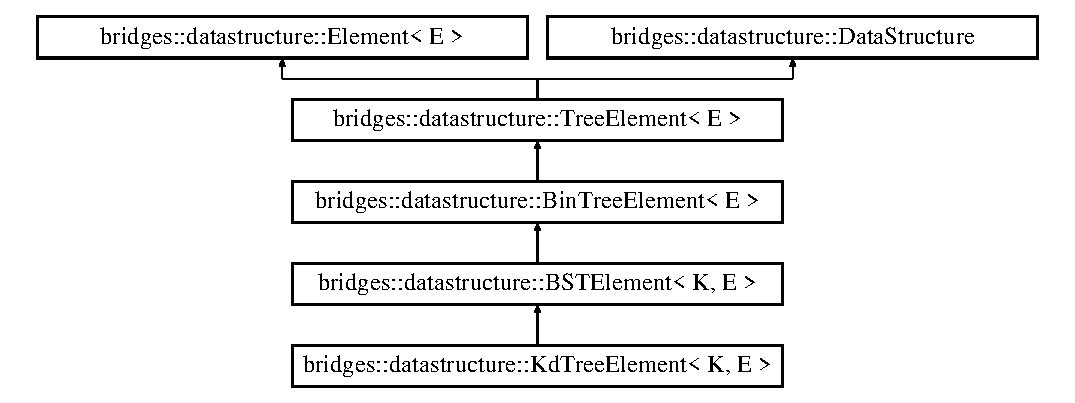
\includegraphics[height=4.964539cm]{classbridges_1_1datastructure_1_1_kd_tree_element}
\end{center}
\end{figure}


\subsection{Detailed Description}
\subsubsection*{template$<$typename K, typename E$>$\newline
class bridges\+::datastructure\+::\+Kd\+Tree\+Element$<$ K, E $>$}

This class can be used to create K-\/d Tree elements, derived from \hyperlink{classbridges_1_1datastructure_1_1_b_s_t_element}{B\+S\+T\+Element}. K-\/D trees can be thought of as the spatial equivalent binary search trees and operate on multiple dimensions (2D and 3D are most common). These trees serve as a representation of the underlying geometrically defined spaces. Specialized versions of these trees include quadtrees and octrees, which subdivide into equal sized quadrants octants at each level, respectively. 

This class extends the \hyperlink{classbridges_1_1datastructure_1_1_b_s_t_element}{B\+S\+T\+Element} class by adding a dimension property. It also includes a thickness property for displaying the partitioning lines generated by the convex decomposition.

convenient to generate visual representation to allow for use in a binary search tree implementation.

Generic Parameters\+: K that is the search key type -\/ this is usually a number, integer or float E the application data type

\begin{DoxyAuthor}{Author}
Kalpathi Subramanian 
\end{DoxyAuthor}
\begin{DoxyDate}{Date}
6/18/15, 7/17/16
\end{DoxyDate}
There is a tutorial about K-\/d Trees \+: \href{http://bridgesuncc.github.io/tutorials/KdTree.html}{\tt http\+://bridgesuncc.\+github.\+io/tutorials/\+Kd\+Tree.\+html} \subsection*{Public Member Functions}
\begin{DoxyCompactItemize}
\item 
\hyperlink{classbridges_1_1datastructure_1_1_kd_tree_element_a5dd9f121e73a5c0643dfb52401472297}{Kd\+Tree\+Element} (const K \&k, int dim, int th, const \hyperlink{classbridges_1_1datastructure_1_1_kd_tree_element}{Kd\+Tree\+Element} $\ast$l, const \hyperlink{classbridges_1_1datastructure_1_1_kd_tree_element}{Kd\+Tree\+Element} $\ast$r, const E \&val=E(), const string \&lab=string())
\item 
\hyperlink{classbridges_1_1datastructure_1_1_kd_tree_element_a5c8f171b78e65a4e07e93282a0f713f6}{Kd\+Tree\+Element} (const K \&k, int dim, int th=0, const E \&val=E(), const string \&lab=string())
\item 
virtual const string \hyperlink{classbridges_1_1datastructure_1_1_kd_tree_element_a76f6d9bfadfdec09d0a8564aa0e33235}{get\+D\+Stype} () const override
\item 
int \hyperlink{classbridges_1_1datastructure_1_1_kd_tree_element_a0321f13830707107198df2d96ff0bc2d}{get\+Dimension} () const
\item 
void \hyperlink{classbridges_1_1datastructure_1_1_kd_tree_element_a9862bde7b85254224963e23dd9bcee29}{set\+Dimension} (const int \&dim)
\item 
virtual \hyperlink{classbridges_1_1datastructure_1_1_kd_tree_element}{Kd\+Tree\+Element} $\ast$ \hyperlink{classbridges_1_1datastructure_1_1_kd_tree_element_a875bfa2dfd88a7740f7bcd28a117c12a}{get\+Left} () override
\item 
virtual const \hyperlink{classbridges_1_1datastructure_1_1_kd_tree_element}{Kd\+Tree\+Element} $\ast$ \hyperlink{classbridges_1_1datastructure_1_1_kd_tree_element_a653597918fbc6e31b84fcf8dbdf67122}{get\+Left} () const override
\item 
void \hyperlink{classbridges_1_1datastructure_1_1_kd_tree_element_a2ca1571186e00b69f73f324bc4c20753}{set\+Left} (\hyperlink{classbridges_1_1datastructure_1_1_kd_tree_element}{Kd\+Tree\+Element} $\ast$l)
\item 
virtual \hyperlink{classbridges_1_1datastructure_1_1_kd_tree_element}{Kd\+Tree\+Element} $\ast$ \hyperlink{classbridges_1_1datastructure_1_1_kd_tree_element_a366e3b0987169220d3a145043be2373d}{get\+Right} () override
\item 
virtual const \hyperlink{classbridges_1_1datastructure_1_1_kd_tree_element}{Kd\+Tree\+Element} $\ast$ \hyperlink{classbridges_1_1datastructure_1_1_kd_tree_element_ae8d6007d3848b72cbfc11d2e29120781}{get\+Right} () const override
\item 
void \hyperlink{classbridges_1_1datastructure_1_1_kd_tree_element_aee269fced2901e0cb580f998457176ca}{set\+Right} (\hyperlink{classbridges_1_1datastructure_1_1_kd_tree_element}{Kd\+Tree\+Element} $\ast$r)
\end{DoxyCompactItemize}
\subsection*{Protected Member Functions}
\begin{DoxyCompactItemize}
\item 
virtual const string \hyperlink{classbridges_1_1datastructure_1_1_kd_tree_element_a5413ecaf152e3df5fb45dd85da812888}{get\+Element\+Representation} () const override
\end{DoxyCompactItemize}
\subsection*{Additional Inherited Members}


\subsection{Constructor \& Destructor Documentation}
\mbox{\Hypertarget{classbridges_1_1datastructure_1_1_kd_tree_element_a5dd9f121e73a5c0643dfb52401472297}\label{classbridges_1_1datastructure_1_1_kd_tree_element_a5dd9f121e73a5c0643dfb52401472297}} 
\index{bridges\+::datastructure\+::\+Kd\+Tree\+Element@{bridges\+::datastructure\+::\+Kd\+Tree\+Element}!Kd\+Tree\+Element@{Kd\+Tree\+Element}}
\index{Kd\+Tree\+Element@{Kd\+Tree\+Element}!bridges\+::datastructure\+::\+Kd\+Tree\+Element@{bridges\+::datastructure\+::\+Kd\+Tree\+Element}}
\subsubsection{\texorpdfstring{Kd\+Tree\+Element()}{KdTreeElement()}\hspace{0.1cm}{\footnotesize\ttfamily [1/2]}}
{\footnotesize\ttfamily template$<$typename K , typename E $>$ \\
\hyperlink{classbridges_1_1datastructure_1_1_kd_tree_element}{bridges\+::datastructure\+::\+Kd\+Tree\+Element}$<$ K, E $>$\+::\hyperlink{classbridges_1_1datastructure_1_1_kd_tree_element}{Kd\+Tree\+Element} (\begin{DoxyParamCaption}\item[{const K \&}]{k,  }\item[{int}]{dim,  }\item[{int}]{th,  }\item[{const \hyperlink{classbridges_1_1datastructure_1_1_kd_tree_element}{Kd\+Tree\+Element}$<$ K, E $>$ $\ast$}]{l,  }\item[{const \hyperlink{classbridges_1_1datastructure_1_1_kd_tree_element}{Kd\+Tree\+Element}$<$ K, E $>$ $\ast$}]{r,  }\item[{const E \&}]{val = {\ttfamily E()},  }\item[{const string \&}]{lab = {\ttfamily string()} }\end{DoxyParamCaption})\hspace{0.3cm}{\ttfamily [inline]}}

Constructs a \hyperlink{classbridges_1_1datastructure_1_1_kd_tree_element}{Kd\+Tree\+Element} with the provided value, label, key, left and right Kd\+Tree elements. The defaults will be used if not provided.


\begin{DoxyParams}{Parameters}
{\em k} & The key for ordering \\
\hline
{\em dim} & number of dimension to be partitioned \\
\hline
{\em th} & thickness of the line showing the partition \\
\hline
{\em l} & The left Kd\+Tree \hyperlink{classbridges_1_1datastructure_1_1_element}{Element} \\
\hline
{\em r} & The right Kd\+Tree \hyperlink{classbridges_1_1datastructure_1_1_element}{Element} \\
\hline
{\em val} & The data to hold \\
\hline
{\em lab} & The label to show \\
\hline
\end{DoxyParams}
\mbox{\Hypertarget{classbridges_1_1datastructure_1_1_kd_tree_element_a5c8f171b78e65a4e07e93282a0f713f6}\label{classbridges_1_1datastructure_1_1_kd_tree_element_a5c8f171b78e65a4e07e93282a0f713f6}} 
\index{bridges\+::datastructure\+::\+Kd\+Tree\+Element@{bridges\+::datastructure\+::\+Kd\+Tree\+Element}!Kd\+Tree\+Element@{Kd\+Tree\+Element}}
\index{Kd\+Tree\+Element@{Kd\+Tree\+Element}!bridges\+::datastructure\+::\+Kd\+Tree\+Element@{bridges\+::datastructure\+::\+Kd\+Tree\+Element}}
\subsubsection{\texorpdfstring{Kd\+Tree\+Element()}{KdTreeElement()}\hspace{0.1cm}{\footnotesize\ttfamily [2/2]}}
{\footnotesize\ttfamily template$<$typename K , typename E $>$ \\
\hyperlink{classbridges_1_1datastructure_1_1_kd_tree_element}{bridges\+::datastructure\+::\+Kd\+Tree\+Element}$<$ K, E $>$\+::\hyperlink{classbridges_1_1datastructure_1_1_kd_tree_element}{Kd\+Tree\+Element} (\begin{DoxyParamCaption}\item[{const K \&}]{k,  }\item[{int}]{dim,  }\item[{int}]{th = {\ttfamily 0},  }\item[{const E \&}]{val = {\ttfamily E()},  }\item[{const string \&}]{lab = {\ttfamily string()} }\end{DoxyParamCaption})\hspace{0.3cm}{\ttfamily [inline]}}

Constructs a \hyperlink{classbridges_1_1datastructure_1_1_kd_tree_element}{Kd\+Tree\+Element} with the provided value, label, key, setting the left and right \hyperlink{classbridges_1_1datastructure_1_1_kd_tree_element}{Kd\+Tree\+Element} to N\+U\+LL. The defaults will be used if not provided.


\begin{DoxyParams}{Parameters}
{\em k} & The key for ordering \\
\hline
{\em dim} & number of dimensions being partitioned \\
\hline
{\em th} & thickness of the line showing the partition \\
\hline
{\em val} & The data to hold \\
\hline
{\em lab} & The label to show \\
\hline
\end{DoxyParams}


\subsection{Member Function Documentation}
\mbox{\Hypertarget{classbridges_1_1datastructure_1_1_kd_tree_element_a0321f13830707107198df2d96ff0bc2d}\label{classbridges_1_1datastructure_1_1_kd_tree_element_a0321f13830707107198df2d96ff0bc2d}} 
\index{bridges\+::datastructure\+::\+Kd\+Tree\+Element@{bridges\+::datastructure\+::\+Kd\+Tree\+Element}!get\+Dimension@{get\+Dimension}}
\index{get\+Dimension@{get\+Dimension}!bridges\+::datastructure\+::\+Kd\+Tree\+Element@{bridges\+::datastructure\+::\+Kd\+Tree\+Element}}
\subsubsection{\texorpdfstring{get\+Dimension()}{getDimension()}}
{\footnotesize\ttfamily template$<$typename K , typename E $>$ \\
int \hyperlink{classbridges_1_1datastructure_1_1_kd_tree_element}{bridges\+::datastructure\+::\+Kd\+Tree\+Element}$<$ K, E $>$\+::get\+Dimension (\begin{DoxyParamCaption}{ }\end{DoxyParamCaption}) const\hspace{0.3cm}{\ttfamily [inline]}}

Get Dimension of the partition \begin{DoxyReturn}{Returns}
return the partitioning of this node 
\end{DoxyReturn}
\mbox{\Hypertarget{classbridges_1_1datastructure_1_1_kd_tree_element_a76f6d9bfadfdec09d0a8564aa0e33235}\label{classbridges_1_1datastructure_1_1_kd_tree_element_a76f6d9bfadfdec09d0a8564aa0e33235}} 
\index{bridges\+::datastructure\+::\+Kd\+Tree\+Element@{bridges\+::datastructure\+::\+Kd\+Tree\+Element}!get\+D\+Stype@{get\+D\+Stype}}
\index{get\+D\+Stype@{get\+D\+Stype}!bridges\+::datastructure\+::\+Kd\+Tree\+Element@{bridges\+::datastructure\+::\+Kd\+Tree\+Element}}
\subsubsection{\texorpdfstring{get\+D\+Stype()}{getDStype()}}
{\footnotesize\ttfamily template$<$typename K , typename E $>$ \\
virtual const string \hyperlink{classbridges_1_1datastructure_1_1_kd_tree_element}{bridges\+::datastructure\+::\+Kd\+Tree\+Element}$<$ K, E $>$\+::get\+D\+Stype (\begin{DoxyParamCaption}{ }\end{DoxyParamCaption}) const\hspace{0.3cm}{\ttfamily [inline]}, {\ttfamily [override]}, {\ttfamily [virtual]}}

\begin{DoxyReturn}{Returns}
the data structure type 
\end{DoxyReturn}


Reimplemented from \hyperlink{classbridges_1_1datastructure_1_1_b_s_t_element_a2bb8cc9ec4b6bc5b89ecef0f17be366f}{bridges\+::datastructure\+::\+B\+S\+T\+Element$<$ K, E $>$}.

\mbox{\Hypertarget{classbridges_1_1datastructure_1_1_kd_tree_element_a5413ecaf152e3df5fb45dd85da812888}\label{classbridges_1_1datastructure_1_1_kd_tree_element_a5413ecaf152e3df5fb45dd85da812888}} 
\index{bridges\+::datastructure\+::\+Kd\+Tree\+Element@{bridges\+::datastructure\+::\+Kd\+Tree\+Element}!get\+Element\+Representation@{get\+Element\+Representation}}
\index{get\+Element\+Representation@{get\+Element\+Representation}!bridges\+::datastructure\+::\+Kd\+Tree\+Element@{bridges\+::datastructure\+::\+Kd\+Tree\+Element}}
\subsubsection{\texorpdfstring{get\+Element\+Representation()}{getElementRepresentation()}}
{\footnotesize\ttfamily template$<$typename K , typename E $>$ \\
virtual const string \hyperlink{classbridges_1_1datastructure_1_1_kd_tree_element}{bridges\+::datastructure\+::\+Kd\+Tree\+Element}$<$ K, E $>$\+::get\+Element\+Representation (\begin{DoxyParamCaption}{ }\end{DoxyParamCaption}) const\hspace{0.3cm}{\ttfamily [inline]}, {\ttfamily [override]}, {\ttfamily [protected]}, {\ttfamily [virtual]}}

Gets the J\+S\+ON representation of this element 

Reimplemented from \hyperlink{classbridges_1_1datastructure_1_1_b_s_t_element_a8f962a01b6e0eff59abeee7768264fd9}{bridges\+::datastructure\+::\+B\+S\+T\+Element$<$ K, E $>$}.

\mbox{\Hypertarget{classbridges_1_1datastructure_1_1_kd_tree_element_a875bfa2dfd88a7740f7bcd28a117c12a}\label{classbridges_1_1datastructure_1_1_kd_tree_element_a875bfa2dfd88a7740f7bcd28a117c12a}} 
\index{bridges\+::datastructure\+::\+Kd\+Tree\+Element@{bridges\+::datastructure\+::\+Kd\+Tree\+Element}!get\+Left@{get\+Left}}
\index{get\+Left@{get\+Left}!bridges\+::datastructure\+::\+Kd\+Tree\+Element@{bridges\+::datastructure\+::\+Kd\+Tree\+Element}}
\subsubsection{\texorpdfstring{get\+Left()}{getLeft()}\hspace{0.1cm}{\footnotesize\ttfamily [1/2]}}
{\footnotesize\ttfamily template$<$typename K , typename E $>$ \\
virtual \hyperlink{classbridges_1_1datastructure_1_1_kd_tree_element}{Kd\+Tree\+Element}$\ast$ \hyperlink{classbridges_1_1datastructure_1_1_kd_tree_element}{bridges\+::datastructure\+::\+Kd\+Tree\+Element}$<$ K, E $>$\+::get\+Left (\begin{DoxyParamCaption}{ }\end{DoxyParamCaption})\hspace{0.3cm}{\ttfamily [inline]}, {\ttfamily [override]}, {\ttfamily [virtual]}}

Get left child \begin{DoxyReturn}{Returns}
The left child 
\end{DoxyReturn}


Reimplemented from \hyperlink{classbridges_1_1datastructure_1_1_b_s_t_element_af863c624691c11db26ae3b6d723d1f5c}{bridges\+::datastructure\+::\+B\+S\+T\+Element$<$ K, E $>$}.

\mbox{\Hypertarget{classbridges_1_1datastructure_1_1_kd_tree_element_a653597918fbc6e31b84fcf8dbdf67122}\label{classbridges_1_1datastructure_1_1_kd_tree_element_a653597918fbc6e31b84fcf8dbdf67122}} 
\index{bridges\+::datastructure\+::\+Kd\+Tree\+Element@{bridges\+::datastructure\+::\+Kd\+Tree\+Element}!get\+Left@{get\+Left}}
\index{get\+Left@{get\+Left}!bridges\+::datastructure\+::\+Kd\+Tree\+Element@{bridges\+::datastructure\+::\+Kd\+Tree\+Element}}
\subsubsection{\texorpdfstring{get\+Left()}{getLeft()}\hspace{0.1cm}{\footnotesize\ttfamily [2/2]}}
{\footnotesize\ttfamily template$<$typename K , typename E $>$ \\
virtual const \hyperlink{classbridges_1_1datastructure_1_1_kd_tree_element}{Kd\+Tree\+Element}$\ast$ \hyperlink{classbridges_1_1datastructure_1_1_kd_tree_element}{bridges\+::datastructure\+::\+Kd\+Tree\+Element}$<$ K, E $>$\+::get\+Left (\begin{DoxyParamCaption}{ }\end{DoxyParamCaption}) const\hspace{0.3cm}{\ttfamily [inline]}, {\ttfamily [override]}, {\ttfamily [virtual]}}

Get left child -\/ constant version

\begin{DoxyReturn}{Returns}
The left child 
\end{DoxyReturn}


Reimplemented from \hyperlink{classbridges_1_1datastructure_1_1_b_s_t_element_abac324ef0b480420bd82ecfe4501d60d}{bridges\+::datastructure\+::\+B\+S\+T\+Element$<$ K, E $>$}.

\mbox{\Hypertarget{classbridges_1_1datastructure_1_1_kd_tree_element_a366e3b0987169220d3a145043be2373d}\label{classbridges_1_1datastructure_1_1_kd_tree_element_a366e3b0987169220d3a145043be2373d}} 
\index{bridges\+::datastructure\+::\+Kd\+Tree\+Element@{bridges\+::datastructure\+::\+Kd\+Tree\+Element}!get\+Right@{get\+Right}}
\index{get\+Right@{get\+Right}!bridges\+::datastructure\+::\+Kd\+Tree\+Element@{bridges\+::datastructure\+::\+Kd\+Tree\+Element}}
\subsubsection{\texorpdfstring{get\+Right()}{getRight()}\hspace{0.1cm}{\footnotesize\ttfamily [1/2]}}
{\footnotesize\ttfamily template$<$typename K , typename E $>$ \\
virtual \hyperlink{classbridges_1_1datastructure_1_1_kd_tree_element}{Kd\+Tree\+Element}$\ast$ \hyperlink{classbridges_1_1datastructure_1_1_kd_tree_element}{bridges\+::datastructure\+::\+Kd\+Tree\+Element}$<$ K, E $>$\+::get\+Right (\begin{DoxyParamCaption}{ }\end{DoxyParamCaption})\hspace{0.3cm}{\ttfamily [inline]}, {\ttfamily [override]}, {\ttfamily [virtual]}}

Get right child \begin{DoxyReturn}{Returns}
The right child 
\end{DoxyReturn}


Reimplemented from \hyperlink{classbridges_1_1datastructure_1_1_b_s_t_element_a80f5085d6d03805dd3091b7693d8e235}{bridges\+::datastructure\+::\+B\+S\+T\+Element$<$ K, E $>$}.

\mbox{\Hypertarget{classbridges_1_1datastructure_1_1_kd_tree_element_ae8d6007d3848b72cbfc11d2e29120781}\label{classbridges_1_1datastructure_1_1_kd_tree_element_ae8d6007d3848b72cbfc11d2e29120781}} 
\index{bridges\+::datastructure\+::\+Kd\+Tree\+Element@{bridges\+::datastructure\+::\+Kd\+Tree\+Element}!get\+Right@{get\+Right}}
\index{get\+Right@{get\+Right}!bridges\+::datastructure\+::\+Kd\+Tree\+Element@{bridges\+::datastructure\+::\+Kd\+Tree\+Element}}
\subsubsection{\texorpdfstring{get\+Right()}{getRight()}\hspace{0.1cm}{\footnotesize\ttfamily [2/2]}}
{\footnotesize\ttfamily template$<$typename K , typename E $>$ \\
virtual const \hyperlink{classbridges_1_1datastructure_1_1_kd_tree_element}{Kd\+Tree\+Element}$\ast$ \hyperlink{classbridges_1_1datastructure_1_1_kd_tree_element}{bridges\+::datastructure\+::\+Kd\+Tree\+Element}$<$ K, E $>$\+::get\+Right (\begin{DoxyParamCaption}{ }\end{DoxyParamCaption}) const\hspace{0.3cm}{\ttfamily [inline]}, {\ttfamily [override]}, {\ttfamily [virtual]}}

Constant version

\begin{DoxyReturn}{Returns}
The right child 
\end{DoxyReturn}


Reimplemented from \hyperlink{classbridges_1_1datastructure_1_1_b_s_t_element_a012f0eb09c3d62b14c73109e6ded0879}{bridges\+::datastructure\+::\+B\+S\+T\+Element$<$ K, E $>$}.

\mbox{\Hypertarget{classbridges_1_1datastructure_1_1_kd_tree_element_a9862bde7b85254224963e23dd9bcee29}\label{classbridges_1_1datastructure_1_1_kd_tree_element_a9862bde7b85254224963e23dd9bcee29}} 
\index{bridges\+::datastructure\+::\+Kd\+Tree\+Element@{bridges\+::datastructure\+::\+Kd\+Tree\+Element}!set\+Dimension@{set\+Dimension}}
\index{set\+Dimension@{set\+Dimension}!bridges\+::datastructure\+::\+Kd\+Tree\+Element@{bridges\+::datastructure\+::\+Kd\+Tree\+Element}}
\subsubsection{\texorpdfstring{set\+Dimension()}{setDimension()}}
{\footnotesize\ttfamily template$<$typename K , typename E $>$ \\
void \hyperlink{classbridges_1_1datastructure_1_1_kd_tree_element}{bridges\+::datastructure\+::\+Kd\+Tree\+Element}$<$ K, E $>$\+::set\+Dimension (\begin{DoxyParamCaption}\item[{const int \&}]{dim }\end{DoxyParamCaption})\hspace{0.3cm}{\ttfamily [inline]}}

Set partitioning dimension to \char`\"{}dim\char`\"{}


\begin{DoxyParams}{Parameters}
{\em dim} & The partitioning dimension of this Kd tree element \\
\hline
\end{DoxyParams}
\mbox{\Hypertarget{classbridges_1_1datastructure_1_1_kd_tree_element_a2ca1571186e00b69f73f324bc4c20753}\label{classbridges_1_1datastructure_1_1_kd_tree_element_a2ca1571186e00b69f73f324bc4c20753}} 
\index{bridges\+::datastructure\+::\+Kd\+Tree\+Element@{bridges\+::datastructure\+::\+Kd\+Tree\+Element}!set\+Left@{set\+Left}}
\index{set\+Left@{set\+Left}!bridges\+::datastructure\+::\+Kd\+Tree\+Element@{bridges\+::datastructure\+::\+Kd\+Tree\+Element}}
\subsubsection{\texorpdfstring{set\+Left()}{setLeft()}}
{\footnotesize\ttfamily template$<$typename K , typename E $>$ \\
void \hyperlink{classbridges_1_1datastructure_1_1_kd_tree_element}{bridges\+::datastructure\+::\+Kd\+Tree\+Element}$<$ K, E $>$\+::set\+Left (\begin{DoxyParamCaption}\item[{\hyperlink{classbridges_1_1datastructure_1_1_kd_tree_element}{Kd\+Tree\+Element}$<$ K, E $>$ $\ast$}]{l }\end{DoxyParamCaption})\hspace{0.3cm}{\ttfamily [inline]}}

Sets left child to \char`\"{}l\char`\"{}


\begin{DoxyParams}{Parameters}
{\em l} & The left child \\
\hline
\end{DoxyParams}
\mbox{\Hypertarget{classbridges_1_1datastructure_1_1_kd_tree_element_aee269fced2901e0cb580f998457176ca}\label{classbridges_1_1datastructure_1_1_kd_tree_element_aee269fced2901e0cb580f998457176ca}} 
\index{bridges\+::datastructure\+::\+Kd\+Tree\+Element@{bridges\+::datastructure\+::\+Kd\+Tree\+Element}!set\+Right@{set\+Right}}
\index{set\+Right@{set\+Right}!bridges\+::datastructure\+::\+Kd\+Tree\+Element@{bridges\+::datastructure\+::\+Kd\+Tree\+Element}}
\subsubsection{\texorpdfstring{set\+Right()}{setRight()}}
{\footnotesize\ttfamily template$<$typename K , typename E $>$ \\
void \hyperlink{classbridges_1_1datastructure_1_1_kd_tree_element}{bridges\+::datastructure\+::\+Kd\+Tree\+Element}$<$ K, E $>$\+::set\+Right (\begin{DoxyParamCaption}\item[{\hyperlink{classbridges_1_1datastructure_1_1_kd_tree_element}{Kd\+Tree\+Element}$<$ K, E $>$ $\ast$}]{r }\end{DoxyParamCaption})\hspace{0.3cm}{\ttfamily [inline]}}

Sets right to \char`\"{}r\char`\"{}


\begin{DoxyParams}{Parameters}
{\em r} & The right \hyperlink{classbridges_1_1datastructure_1_1_b_s_t_element}{B\+S\+T\+Element} \\
\hline
\end{DoxyParams}


The documentation for this class was generated from the following file\+:\begin{DoxyCompactItemize}
\item 
/home/erik/work/bridges/bridges-\/cxx/src/\hyperlink{_kd_tree_element_8h}{Kd\+Tree\+Element.\+h}\end{DoxyCompactItemize}

\hypertarget{classbridges_1_1game_1_1_keypress_listener}{}\section{bridges\+::game\+::Keypress\+Listener Class Reference}
\label{classbridges_1_1game_1_1_keypress_listener}\index{bridges::game::KeypressListener@{bridges::game::KeypressListener}}


{\ttfamily \#include $<$Socket\+Connection.\+h$>$}

Inheritance diagram for bridges\+::game\+::Keypress\+Listener\+:\begin{figure}[H]
\begin{center}
\leavevmode
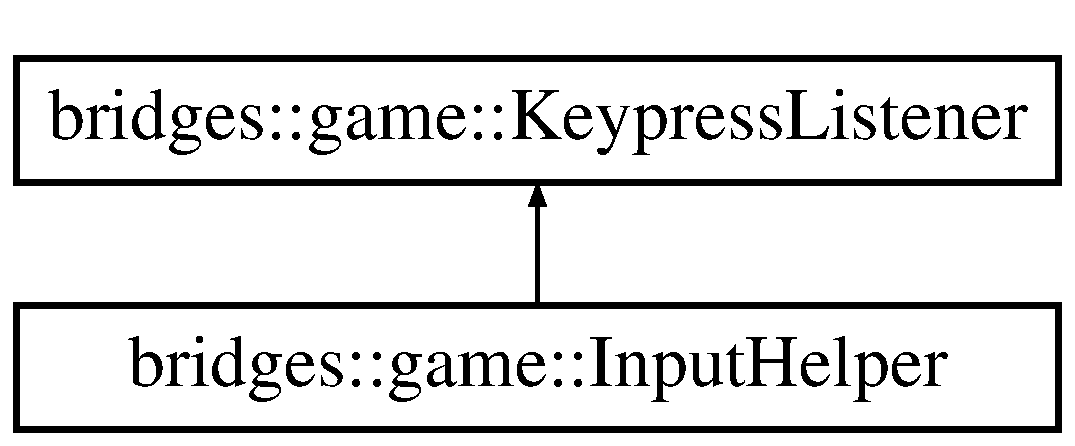
\includegraphics[height=2.000000cm]{classbridges_1_1game_1_1_keypress_listener}
\end{center}
\end{figure}
\subsection*{Public Member Functions}
\begin{DoxyCompactItemize}
\item 
virtual void \mbox{\hyperlink{classbridges_1_1game_1_1_keypress_listener_a21d9f085819e30c41f3964ea2276964d}{keyup}} (std\+::string J\+S\+O\+Nmessage)=0
\item 
virtual void \mbox{\hyperlink{classbridges_1_1game_1_1_keypress_listener_a79362f390cad37bfe73012a05599e8aa}{keydown}} (std\+::string J\+S\+O\+Nmessage)=0
\end{DoxyCompactItemize}


\subsection{Member Function Documentation}
\mbox{\Hypertarget{classbridges_1_1game_1_1_keypress_listener_a79362f390cad37bfe73012a05599e8aa}\label{classbridges_1_1game_1_1_keypress_listener_a79362f390cad37bfe73012a05599e8aa}} 
\index{bridges::game::KeypressListener@{bridges::game::KeypressListener}!keydown@{keydown}}
\index{keydown@{keydown}!bridges::game::KeypressListener@{bridges::game::KeypressListener}}
\subsubsection{\texorpdfstring{keydown()}{keydown()}}
{\footnotesize\ttfamily virtual void bridges\+::game\+::\+Keypress\+Listener\+::keydown (\begin{DoxyParamCaption}\item[{std\+::string}]{J\+S\+O\+Nmessage }\end{DoxyParamCaption})\hspace{0.3cm}{\ttfamily [pure virtual]}}



Implemented in \mbox{\hyperlink{classbridges_1_1game_1_1_input_helper_aac75c2b1abf28afa4acaf730e925f301}{bridges\+::game\+::\+Input\+Helper}}.

\mbox{\Hypertarget{classbridges_1_1game_1_1_keypress_listener_a21d9f085819e30c41f3964ea2276964d}\label{classbridges_1_1game_1_1_keypress_listener_a21d9f085819e30c41f3964ea2276964d}} 
\index{bridges::game::KeypressListener@{bridges::game::KeypressListener}!keyup@{keyup}}
\index{keyup@{keyup}!bridges::game::KeypressListener@{bridges::game::KeypressListener}}
\subsubsection{\texorpdfstring{keyup()}{keyup()}}
{\footnotesize\ttfamily virtual void bridges\+::game\+::\+Keypress\+Listener\+::keyup (\begin{DoxyParamCaption}\item[{std\+::string}]{J\+S\+O\+Nmessage }\end{DoxyParamCaption})\hspace{0.3cm}{\ttfamily [pure virtual]}}



Implemented in \mbox{\hyperlink{classbridges_1_1game_1_1_input_helper_aa847f19c6f68ebbb63d73802abfcd9a0}{bridges\+::game\+::\+Input\+Helper}}.



The documentation for this class was generated from the following file\+:\begin{DoxyCompactItemize}
\item 
/\+Users/kalpathi/gr/bridges/cxx/src/\mbox{\hyperlink{_socket_connection_8h}{Socket\+Connection.\+h}}\end{DoxyCompactItemize}

\hypertarget{classbridges_1_1datastructure_1_1_graph_adj_list_1_1_key_set__helper}{}\section{bridges\+:\+:datastructure\+:\+:Graph\+Adj\+List$<$ K, E1, E2 $>$\+:\+:Key\+Set\+\_\+helper Class Reference}
\label{classbridges_1_1datastructure_1_1_graph_adj_list_1_1_key_set__helper}\index{bridges\+::datastructure\+::\+Graph\+Adj\+List$<$ K, E1, E2 $>$\+::\+Key\+Set\+\_\+helper@{bridges\+::datastructure\+::\+Graph\+Adj\+List$<$ K, E1, E2 $>$\+::\+Key\+Set\+\_\+helper}}


{\ttfamily \#include $<$Graph\+Adj\+List.\+h$>$}



\subsection{Detailed Description}
\subsubsection*{template$<$typename K, typename E1 = K, typename E2 = E1$>$\newline
class bridges\+::datastructure\+::\+Graph\+Adj\+List$<$ K, E1, E2 $>$\+::\+Key\+Set\+\_\+helper}

This is a helper class to return sets of vertices ina way that are iterable with range for loops. Students should not have to use this directly. \subsection*{Classes}
\begin{DoxyCompactItemize}
\item 
class \hyperlink{classbridges_1_1datastructure_1_1_graph_adj_list_1_1_key_set__helper_1_1const__iterator}{const\+\_\+iterator}
\end{DoxyCompactItemize}
\subsection*{Public Member Functions}
\begin{DoxyCompactItemize}
\item 
\hyperlink{classbridges_1_1datastructure_1_1_graph_adj_list_1_1_key_set__helper_a62d14661afdef7ae642c3f1d47ddc871}{Key\+Set\+\_\+helper} (std\+::unordered\+\_\+map$<$ K, \hyperlink{classbridges_1_1datastructure_1_1_element}{Element}$<$ E1 $>$ $\ast$ $>$ const \&um)
\item 
\hyperlink{classbridges_1_1datastructure_1_1_graph_adj_list_1_1_key_set__helper_1_1const__iterator}{const\+\_\+iterator} \hyperlink{classbridges_1_1datastructure_1_1_graph_adj_list_1_1_key_set__helper_a862efabcacc55dab2c383485fb10fd85}{begin} () const
\item 
\hyperlink{classbridges_1_1datastructure_1_1_graph_adj_list_1_1_key_set__helper_1_1const__iterator}{const\+\_\+iterator} \hyperlink{classbridges_1_1datastructure_1_1_graph_adj_list_1_1_key_set__helper_a6204f2d6c81b2b4cc72387cbce6c4f0d}{end} () const
\end{DoxyCompactItemize}


\subsection{Constructor \& Destructor Documentation}
\mbox{\Hypertarget{classbridges_1_1datastructure_1_1_graph_adj_list_1_1_key_set__helper_a62d14661afdef7ae642c3f1d47ddc871}\label{classbridges_1_1datastructure_1_1_graph_adj_list_1_1_key_set__helper_a62d14661afdef7ae642c3f1d47ddc871}} 
\index{bridges\+::datastructure\+::\+Graph\+Adj\+List\+::\+Key\+Set\+\_\+helper@{bridges\+::datastructure\+::\+Graph\+Adj\+List\+::\+Key\+Set\+\_\+helper}!Key\+Set\+\_\+helper@{Key\+Set\+\_\+helper}}
\index{Key\+Set\+\_\+helper@{Key\+Set\+\_\+helper}!bridges\+::datastructure\+::\+Graph\+Adj\+List\+::\+Key\+Set\+\_\+helper@{bridges\+::datastructure\+::\+Graph\+Adj\+List\+::\+Key\+Set\+\_\+helper}}
\subsubsection{\texorpdfstring{Key\+Set\+\_\+helper()}{KeySet\_helper()}}
{\footnotesize\ttfamily template$<$typename K, typename E1 = K, typename E2 = E1$>$ \\
\hyperlink{classbridges_1_1datastructure_1_1_graph_adj_list}{bridges\+::datastructure\+::\+Graph\+Adj\+List}$<$ K, E1, E2 $>$\+::Key\+Set\+\_\+helper\+::\+Key\+Set\+\_\+helper (\begin{DoxyParamCaption}\item[{std\+::unordered\+\_\+map$<$ K, \hyperlink{classbridges_1_1datastructure_1_1_element}{Element}$<$ E1 $>$ $\ast$ $>$ const \&}]{um }\end{DoxyParamCaption})\hspace{0.3cm}{\ttfamily [inline]}}



\subsection{Member Function Documentation}
\mbox{\Hypertarget{classbridges_1_1datastructure_1_1_graph_adj_list_1_1_key_set__helper_a862efabcacc55dab2c383485fb10fd85}\label{classbridges_1_1datastructure_1_1_graph_adj_list_1_1_key_set__helper_a862efabcacc55dab2c383485fb10fd85}} 
\index{bridges\+::datastructure\+::\+Graph\+Adj\+List\+::\+Key\+Set\+\_\+helper@{bridges\+::datastructure\+::\+Graph\+Adj\+List\+::\+Key\+Set\+\_\+helper}!begin@{begin}}
\index{begin@{begin}!bridges\+::datastructure\+::\+Graph\+Adj\+List\+::\+Key\+Set\+\_\+helper@{bridges\+::datastructure\+::\+Graph\+Adj\+List\+::\+Key\+Set\+\_\+helper}}
\subsubsection{\texorpdfstring{begin()}{begin()}}
{\footnotesize\ttfamily template$<$typename K, typename E1 = K, typename E2 = E1$>$ \\
\hyperlink{classbridges_1_1datastructure_1_1_graph_adj_list_1_1_key_set__helper_1_1const__iterator}{const\+\_\+iterator} \hyperlink{classbridges_1_1datastructure_1_1_graph_adj_list}{bridges\+::datastructure\+::\+Graph\+Adj\+List}$<$ K, E1, E2 $>$\+::Key\+Set\+\_\+helper\+::begin (\begin{DoxyParamCaption}{ }\end{DoxyParamCaption}) const\hspace{0.3cm}{\ttfamily [inline]}}

\mbox{\Hypertarget{classbridges_1_1datastructure_1_1_graph_adj_list_1_1_key_set__helper_a6204f2d6c81b2b4cc72387cbce6c4f0d}\label{classbridges_1_1datastructure_1_1_graph_adj_list_1_1_key_set__helper_a6204f2d6c81b2b4cc72387cbce6c4f0d}} 
\index{bridges\+::datastructure\+::\+Graph\+Adj\+List\+::\+Key\+Set\+\_\+helper@{bridges\+::datastructure\+::\+Graph\+Adj\+List\+::\+Key\+Set\+\_\+helper}!end@{end}}
\index{end@{end}!bridges\+::datastructure\+::\+Graph\+Adj\+List\+::\+Key\+Set\+\_\+helper@{bridges\+::datastructure\+::\+Graph\+Adj\+List\+::\+Key\+Set\+\_\+helper}}
\subsubsection{\texorpdfstring{end()}{end()}}
{\footnotesize\ttfamily template$<$typename K, typename E1 = K, typename E2 = E1$>$ \\
\hyperlink{classbridges_1_1datastructure_1_1_graph_adj_list_1_1_key_set__helper_1_1const__iterator}{const\+\_\+iterator} \hyperlink{classbridges_1_1datastructure_1_1_graph_adj_list}{bridges\+::datastructure\+::\+Graph\+Adj\+List}$<$ K, E1, E2 $>$\+::Key\+Set\+\_\+helper\+::end (\begin{DoxyParamCaption}{ }\end{DoxyParamCaption}) const\hspace{0.3cm}{\ttfamily [inline]}}



The documentation for this class was generated from the following file\+:\begin{DoxyCompactItemize}
\item 
/home/erik/work/bridges/bridges-\/cxx/src/\hyperlink{_graph_adj_list_8h}{Graph\+Adj\+List.\+h}\end{DoxyCompactItemize}

\hypertarget{classbridges_1_1datastructure_1_1_label}{}\section{bridges\+::datastructure\+::Label Class Reference}
\label{classbridges_1_1datastructure_1_1_label}\index{bridges::datastructure::Label@{bridges::datastructure::Label}}


{\ttfamily \#include $<$Label.\+h$>$}

Inheritance diagram for bridges\+::datastructure\+::Label\+:\begin{figure}[H]
\begin{center}
\leavevmode
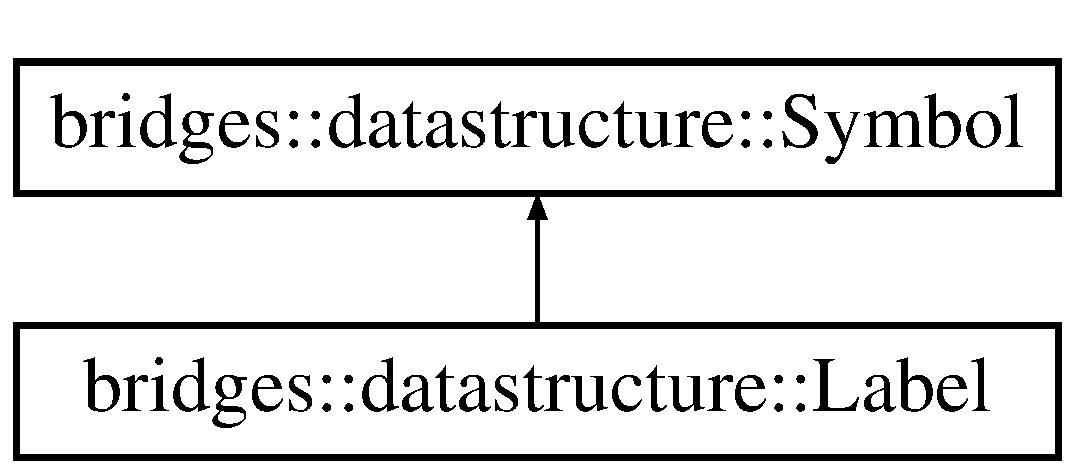
\includegraphics[height=2.000000cm]{classbridges_1_1datastructure_1_1_label}
\end{center}
\end{figure}


\subsection{Detailed Description}
This is a label object and used for defining text labels as part of the symbol collection. 

\begin{DoxyAuthor}{Author}
Kalpathi Subramanian 
\end{DoxyAuthor}
\begin{DoxyDate}{Date}
12/23/18 
\end{DoxyDate}
\subsection*{Public Member Functions}
\begin{DoxyCompactItemize}
\item 
\mbox{\hyperlink{classbridges_1_1datastructure_1_1_label_abd73b3f555e6de007b7cb82cdf7c57cd}{Label}} ()
\item 
\mbox{\hyperlink{classbridges_1_1datastructure_1_1_label_a2eacf0820ea29c309f4910db5756607c}{Label}} (string l)
\item 
string \mbox{\hyperlink{classbridges_1_1datastructure_1_1_label_a55ccc4e52bd1f09c55ba6b775e7768ab}{get\+Data\+Struct\+Type}} ()
\item 
string \mbox{\hyperlink{classbridges_1_1datastructure_1_1_label_ac2a15e34404b9b7859e658da63a7020f}{get\+Name}} () const
\item 
void \mbox{\hyperlink{classbridges_1_1datastructure_1_1_label_aee5cc86a51a237c87e56db8e02d271b1}{set\+Font\+Size}} (int sz)
\item 
int \mbox{\hyperlink{classbridges_1_1datastructure_1_1_label_a200cc9710f28af2e63738d5166eaa51f}{get\+Font\+Size}} ()
\item 
void \mbox{\hyperlink{classbridges_1_1datastructure_1_1_label_a323af06f4536c644d6cc265b332b6ad0}{set\+Text\+Width}} (int w)
\item 
int \mbox{\hyperlink{classbridges_1_1datastructure_1_1_label_ab97fecf82c0c21f870f4dc25b6244099}{get\+Text\+Width}} ()
\item 
void \mbox{\hyperlink{classbridges_1_1datastructure_1_1_label_acd095180b94bad422f7c26182680a958}{set\+Text\+Height}} (int h)
\item 
int \mbox{\hyperlink{classbridges_1_1datastructure_1_1_label_aeaf64e048094d69e11e77563c598a045}{get\+Text\+Height}} ()
\item 
vector$<$ float $>$ \mbox{\hyperlink{classbridges_1_1datastructure_1_1_label_ac8f5e0d05c8f4466b3bf07e1fa342091}{get\+Dimensions}} ()
\item 
const string \mbox{\hyperlink{classbridges_1_1datastructure_1_1_label_aa3b7c9e5630ecc8a2534e6db2a220e90}{get\+Symbol\+Representation}} () const
\end{DoxyCompactItemize}
\subsection*{Additional Inherited Members}


\subsection{Constructor \& Destructor Documentation}
\mbox{\Hypertarget{classbridges_1_1datastructure_1_1_label_abd73b3f555e6de007b7cb82cdf7c57cd}\label{classbridges_1_1datastructure_1_1_label_abd73b3f555e6de007b7cb82cdf7c57cd}} 
\index{bridges::datastructure::Label@{bridges::datastructure::Label}!Label@{Label}}
\index{Label@{Label}!bridges::datastructure::Label@{bridges::datastructure::Label}}
\subsubsection{\texorpdfstring{Label()}{Label()}\hspace{0.1cm}{\footnotesize\ttfamily [1/2]}}
{\footnotesize\ttfamily bridges\+::datastructure\+::\+Label\+::\+Label (\begin{DoxyParamCaption}{ }\end{DoxyParamCaption})\hspace{0.3cm}{\ttfamily [inline]}}

constructors \mbox{\Hypertarget{classbridges_1_1datastructure_1_1_label_a2eacf0820ea29c309f4910db5756607c}\label{classbridges_1_1datastructure_1_1_label_a2eacf0820ea29c309f4910db5756607c}} 
\index{bridges::datastructure::Label@{bridges::datastructure::Label}!Label@{Label}}
\index{Label@{Label}!bridges::datastructure::Label@{bridges::datastructure::Label}}
\subsubsection{\texorpdfstring{Label()}{Label()}\hspace{0.1cm}{\footnotesize\ttfamily [2/2]}}
{\footnotesize\ttfamily bridges\+::datastructure\+::\+Label\+::\+Label (\begin{DoxyParamCaption}\item[{string}]{l }\end{DoxyParamCaption})\hspace{0.3cm}{\ttfamily [inline]}}

Create a label object with label l


\begin{DoxyParams}{Parameters}
{\em l} & label \\
\hline
\end{DoxyParams}


\subsection{Member Function Documentation}
\mbox{\Hypertarget{classbridges_1_1datastructure_1_1_label_a55ccc4e52bd1f09c55ba6b775e7768ab}\label{classbridges_1_1datastructure_1_1_label_a55ccc4e52bd1f09c55ba6b775e7768ab}} 
\index{bridges::datastructure::Label@{bridges::datastructure::Label}!getDataStructType@{getDataStructType}}
\index{getDataStructType@{getDataStructType}!bridges::datastructure::Label@{bridges::datastructure::Label}}
\subsubsection{\texorpdfstring{getDataStructType()}{getDataStructType()}}
{\footnotesize\ttfamily string bridges\+::datastructure\+::\+Label\+::get\+Data\+Struct\+Type (\begin{DoxyParamCaption}{ }\end{DoxyParamCaption})\hspace{0.3cm}{\ttfamily [inline]}}

\mbox{\Hypertarget{classbridges_1_1datastructure_1_1_label_ac8f5e0d05c8f4466b3bf07e1fa342091}\label{classbridges_1_1datastructure_1_1_label_ac8f5e0d05c8f4466b3bf07e1fa342091}} 
\index{bridges::datastructure::Label@{bridges::datastructure::Label}!getDimensions@{getDimensions}}
\index{getDimensions@{getDimensions}!bridges::datastructure::Label@{bridges::datastructure::Label}}
\subsubsection{\texorpdfstring{getDimensions()}{getDimensions()}}
{\footnotesize\ttfamily vector$<$float$>$ bridges\+::datastructure\+::\+Label\+::get\+Dimensions (\begin{DoxyParamCaption}{ }\end{DoxyParamCaption})\hspace{0.3cm}{\ttfamily [inline]}, {\ttfamily [virtual]}}

This method returns the bounding box dimensions of the shape

\begin{DoxyReturn}{Returns}
vector of floats 
\end{DoxyReturn}


Implements \mbox{\hyperlink{classbridges_1_1datastructure_1_1_symbol_a37ba60b6acdd0888677eb8c64a931679}{bridges\+::datastructure\+::\+Symbol}}.

\mbox{\Hypertarget{classbridges_1_1datastructure_1_1_label_a200cc9710f28af2e63738d5166eaa51f}\label{classbridges_1_1datastructure_1_1_label_a200cc9710f28af2e63738d5166eaa51f}} 
\index{bridges::datastructure::Label@{bridges::datastructure::Label}!getFontSize@{getFontSize}}
\index{getFontSize@{getFontSize}!bridges::datastructure::Label@{bridges::datastructure::Label}}
\subsubsection{\texorpdfstring{getFontSize()}{getFontSize()}}
{\footnotesize\ttfamily int bridges\+::datastructure\+::\+Label\+::get\+Font\+Size (\begin{DoxyParamCaption}{ }\end{DoxyParamCaption})\hspace{0.3cm}{\ttfamily [inline]}}

This method gets the font size

\begin{DoxyReturn}{Returns}
font size 
\end{DoxyReturn}
\mbox{\Hypertarget{classbridges_1_1datastructure_1_1_label_ac2a15e34404b9b7859e658da63a7020f}\label{classbridges_1_1datastructure_1_1_label_ac2a15e34404b9b7859e658da63a7020f}} 
\index{bridges::datastructure::Label@{bridges::datastructure::Label}!getName@{getName}}
\index{getName@{getName}!bridges::datastructure::Label@{bridges::datastructure::Label}}
\subsubsection{\texorpdfstring{getName()}{getName()}}
{\footnotesize\ttfamily string bridges\+::datastructure\+::\+Label\+::get\+Name (\begin{DoxyParamCaption}{ }\end{DoxyParamCaption}) const\hspace{0.3cm}{\ttfamily [inline]}}

This method gets the name of the shape

\begin{DoxyReturn}{Returns}
name shape name 
\end{DoxyReturn}
\mbox{\Hypertarget{classbridges_1_1datastructure_1_1_label_aa3b7c9e5630ecc8a2534e6db2a220e90}\label{classbridges_1_1datastructure_1_1_label_aa3b7c9e5630ecc8a2534e6db2a220e90}} 
\index{bridges::datastructure::Label@{bridges::datastructure::Label}!getSymbolRepresentation@{getSymbolRepresentation}}
\index{getSymbolRepresentation@{getSymbolRepresentation}!bridges::datastructure::Label@{bridges::datastructure::Label}}
\subsubsection{\texorpdfstring{getSymbolRepresentation()}{getSymbolRepresentation()}}
{\footnotesize\ttfamily const string bridges\+::datastructure\+::\+Label\+::get\+Symbol\+Representation (\begin{DoxyParamCaption}{ }\end{DoxyParamCaption}) const\hspace{0.3cm}{\ttfamily [inline]}, {\ttfamily [virtual]}}

This method returns the J\+S\+ON representation of the shape

\begin{DoxyReturn}{Returns}
string J\+S\+ON string 
\end{DoxyReturn}


Implements \mbox{\hyperlink{classbridges_1_1datastructure_1_1_symbol_a8044b3da559dcd9de8510ae339f126c8}{bridges\+::datastructure\+::\+Symbol}}.

\mbox{\Hypertarget{classbridges_1_1datastructure_1_1_label_aeaf64e048094d69e11e77563c598a045}\label{classbridges_1_1datastructure_1_1_label_aeaf64e048094d69e11e77563c598a045}} 
\index{bridges::datastructure::Label@{bridges::datastructure::Label}!getTextHeight@{getTextHeight}}
\index{getTextHeight@{getTextHeight}!bridges::datastructure::Label@{bridges::datastructure::Label}}
\subsubsection{\texorpdfstring{getTextHeight()}{getTextHeight()}}
{\footnotesize\ttfamily int bridges\+::datastructure\+::\+Label\+::get\+Text\+Height (\begin{DoxyParamCaption}{ }\end{DoxyParamCaption})\hspace{0.3cm}{\ttfamily [inline]}}

This method gets the text height

\begin{DoxyReturn}{Returns}
text height 
\end{DoxyReturn}
\mbox{\Hypertarget{classbridges_1_1datastructure_1_1_label_ab97fecf82c0c21f870f4dc25b6244099}\label{classbridges_1_1datastructure_1_1_label_ab97fecf82c0c21f870f4dc25b6244099}} 
\index{bridges::datastructure::Label@{bridges::datastructure::Label}!getTextWidth@{getTextWidth}}
\index{getTextWidth@{getTextWidth}!bridges::datastructure::Label@{bridges::datastructure::Label}}
\subsubsection{\texorpdfstring{getTextWidth()}{getTextWidth()}}
{\footnotesize\ttfamily int bridges\+::datastructure\+::\+Label\+::get\+Text\+Width (\begin{DoxyParamCaption}{ }\end{DoxyParamCaption})\hspace{0.3cm}{\ttfamily [inline]}}

This method gets the text width

\begin{DoxyReturn}{Returns}
text width 
\end{DoxyReturn}
\mbox{\Hypertarget{classbridges_1_1datastructure_1_1_label_aee5cc86a51a237c87e56db8e02d271b1}\label{classbridges_1_1datastructure_1_1_label_aee5cc86a51a237c87e56db8e02d271b1}} 
\index{bridges::datastructure::Label@{bridges::datastructure::Label}!setFontSize@{setFontSize}}
\index{setFontSize@{setFontSize}!bridges::datastructure::Label@{bridges::datastructure::Label}}
\subsubsection{\texorpdfstring{setFontSize()}{setFontSize()}}
{\footnotesize\ttfamily void bridges\+::datastructure\+::\+Label\+::set\+Font\+Size (\begin{DoxyParamCaption}\item[{int}]{sz }\end{DoxyParamCaption})\hspace{0.3cm}{\ttfamily [inline]}}

This method sets the font size


\begin{DoxyParams}{Parameters}
{\em sz} & font size \\
\hline
\end{DoxyParams}
\mbox{\Hypertarget{classbridges_1_1datastructure_1_1_label_acd095180b94bad422f7c26182680a958}\label{classbridges_1_1datastructure_1_1_label_acd095180b94bad422f7c26182680a958}} 
\index{bridges::datastructure::Label@{bridges::datastructure::Label}!setTextHeight@{setTextHeight}}
\index{setTextHeight@{setTextHeight}!bridges::datastructure::Label@{bridges::datastructure::Label}}
\subsubsection{\texorpdfstring{setTextHeight()}{setTextHeight()}}
{\footnotesize\ttfamily void bridges\+::datastructure\+::\+Label\+::set\+Text\+Height (\begin{DoxyParamCaption}\item[{int}]{h }\end{DoxyParamCaption})\hspace{0.3cm}{\ttfamily [inline]}}

This method sets the text height


\begin{DoxyParams}{Parameters}
{\em h} & text height \\
\hline
\end{DoxyParams}
\mbox{\Hypertarget{classbridges_1_1datastructure_1_1_label_a323af06f4536c644d6cc265b332b6ad0}\label{classbridges_1_1datastructure_1_1_label_a323af06f4536c644d6cc265b332b6ad0}} 
\index{bridges::datastructure::Label@{bridges::datastructure::Label}!setTextWidth@{setTextWidth}}
\index{setTextWidth@{setTextWidth}!bridges::datastructure::Label@{bridges::datastructure::Label}}
\subsubsection{\texorpdfstring{setTextWidth()}{setTextWidth()}}
{\footnotesize\ttfamily void bridges\+::datastructure\+::\+Label\+::set\+Text\+Width (\begin{DoxyParamCaption}\item[{int}]{w }\end{DoxyParamCaption})\hspace{0.3cm}{\ttfamily [inline]}}

This method sets the text width


\begin{DoxyParams}{Parameters}
{\em w} & text width \\
\hline
\end{DoxyParams}


The documentation for this class was generated from the following file\+:\begin{DoxyCompactItemize}
\item 
/\+Users/kalpathi/gr/bridges/cxx/src/\mbox{\hyperlink{_label_8h}{Label.\+h}}\end{DoxyCompactItemize}

\hypertarget{classbridges_1_1datastructure_1_1_line_chart}{}\section{bridges\+:\+:datastructure\+:\+:Line\+Chart Class Reference}
\label{classbridges_1_1datastructure_1_1_line_chart}\index{bridges\+::datastructure\+::\+Line\+Chart@{bridges\+::datastructure\+::\+Line\+Chart}}


{\ttfamily \#include $<$Line\+Chart.\+h$>$}

Inheritance diagram for bridges\+:\+:datastructure\+:\+:Line\+Chart\+:\begin{figure}[H]
\begin{center}
\leavevmode
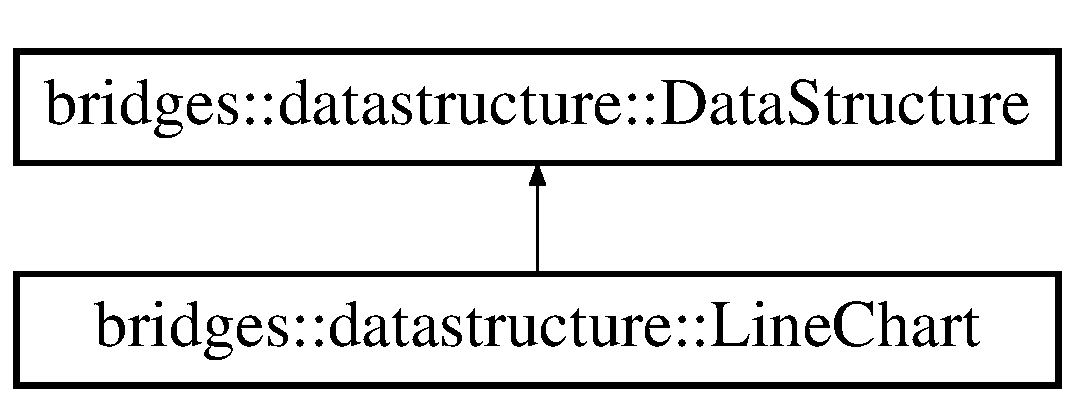
\includegraphics[height=2.000000cm]{classbridges_1_1datastructure_1_1_line_chart}
\end{center}
\end{figure}


\subsection{Detailed Description}
Show series of data or functions using a line chart. 

Line charts (\href{https://en.wikipedia.org/wiki/Line_chart}{\tt https\+://en.\+wikipedia.\+org/wiki/\+Line\+\_\+chart}) are used to represent graphically functions such as f(x) = 3$\ast$x+1, or data such as temperature of a liquid on a stove as time passes. A individual function or a set of data is called \char`\"{}series\char`\"{}.

A series is represented by two arrays xdata and ydata such that there is a point at (xdata\mbox{[}0\mbox{]}, ydata\mbox{[}0\mbox{]}), an other at (xdata\mbox{[}1\mbox{]}, ydata\mbox{[}1\mbox{]}), ... One can add a series by passing the two arrays using \mbox{\hyperlink{classbridges_1_1datastructure_1_1_line_chart_acb763ea4b2d0f27c73edc3861cc51fbb}{set\+Data\+Series()}} or add the arrays individually using \mbox{\hyperlink{classbridges_1_1datastructure_1_1_line_chart_aa9959489d71e31645f561c4481f050d2}{set\+X\+Data()}} and \mbox{\hyperlink{classbridges_1_1datastructure_1_1_line_chart_a861370f3f7b32cc1a9347727d084d307}{set\+Y\+Data()}}.

The different series have a label associated with them by default which can be disabled (see \mbox{\hyperlink{classbridges_1_1datastructure_1_1_line_chart_a21031cd026426ab91307626ce9651c03}{toggle\+Series\+Label()}}).

The data is typically shown with axes that use a linear scale. However, the scale can be changed to logarithmic for each axis individually (see \mbox{\hyperlink{classbridges_1_1datastructure_1_1_line_chart_a4e2aa224d793793faa0c5a6edb729646}{toggle\+Logarithmic\+X()}} and toggle\+Logarithmic()).

The \mbox{\hyperlink{classbridges_1_1datastructure_1_1_line_chart}{Line\+Chart}} can have a title (see \mbox{\hyperlink{classbridges_1_1datastructure_1_1_line_chart_aa38d6cf9657d2757a98b657f079ae2bc}{get\+Title()}} and \mbox{\hyperlink{classbridges_1_1datastructure_1_1_line_chart_ac42cf1e6348ce8ab0c3593a496a3539c}{set\+Title()}}) and a subtitle (see \mbox{\hyperlink{classbridges_1_1datastructure_1_1_line_chart_a578c2590cb6baa8ef40ba1251bd1279e}{set\+Sub\+Title()}} and \mbox{\hyperlink{classbridges_1_1datastructure_1_1_line_chart_a07a4424d4bbc1cdd15cef3e2c0f0c075}{get\+Sub\+Title()}}).

\begin{DoxyAuthor}{Author}
Erik Saule, Kalpathi Subramanian
\end{DoxyAuthor}
\begin{DoxyDate}{Date}
7/16/19 
\end{DoxyDate}
\subsection*{Public Member Functions}
\begin{DoxyCompactItemize}
\item 
\mbox{\hyperlink{classbridges_1_1datastructure_1_1_line_chart_ab96c0639aca0d08c19e5d3b51a29b0a6}{Line\+Chart}} ()
\item 
virtual const string \mbox{\hyperlink{classbridges_1_1datastructure_1_1_line_chart_a431e49c31cdd5f46e978742776306dfa}{get\+D\+Stype}} () const override
\begin{DoxyCompactList}\small\item\em Get the data type. \end{DoxyCompactList}\item 
void \mbox{\hyperlink{classbridges_1_1datastructure_1_1_line_chart_aece56ea5afaf10037b698673801c4496}{toggle\+Mouse\+Track}} (bool val)
\begin{DoxyCompactList}\small\item\em Enables or disables mouse tracking. \end{DoxyCompactList}\item 
void \mbox{\hyperlink{classbridges_1_1datastructure_1_1_line_chart_a21031cd026426ab91307626ce9651c03}{toggle\+Series\+Label}} (bool val)
\begin{DoxyCompactList}\small\item\em Enables or disables series labels. \end{DoxyCompactList}\item 
void \mbox{\hyperlink{classbridges_1_1datastructure_1_1_line_chart_a4e2aa224d793793faa0c5a6edb729646}{toggle\+LogarithmicX}} (bool val)
\begin{DoxyCompactList}\small\item\em Change the X-\/axis scale to logarithmic. \end{DoxyCompactList}\item 
void \mbox{\hyperlink{classbridges_1_1datastructure_1_1_line_chart_a30c72748323d3da25974b30e11e46f48}{toggle\+LogarithmicY}} (bool val)
\begin{DoxyCompactList}\small\item\em Change the Y-\/axis scale to logarithmic. \end{DoxyCompactList}\item 
void \mbox{\hyperlink{classbridges_1_1datastructure_1_1_line_chart_ac42cf1e6348ce8ab0c3593a496a3539c}{set\+Title}} (string t)
\begin{DoxyCompactList}\small\item\em Title of the plot. \end{DoxyCompactList}\item 
string \mbox{\hyperlink{classbridges_1_1datastructure_1_1_line_chart_aa38d6cf9657d2757a98b657f079ae2bc}{get\+Title}} () const
\begin{DoxyCompactList}\small\item\em Title of the plot. \end{DoxyCompactList}\item 
void \mbox{\hyperlink{classbridges_1_1datastructure_1_1_line_chart_a578c2590cb6baa8ef40ba1251bd1279e}{set\+Sub\+Title}} (string s)
\begin{DoxyCompactList}\small\item\em Subtitle of the plot. \end{DoxyCompactList}\item 
string \mbox{\hyperlink{classbridges_1_1datastructure_1_1_line_chart_a07a4424d4bbc1cdd15cef3e2c0f0c075}{get\+Sub\+Title}} () const
\begin{DoxyCompactList}\small\item\em Subtitle of the plot. \end{DoxyCompactList}\item 
void \mbox{\hyperlink{classbridges_1_1datastructure_1_1_line_chart_ac41be5abf80052f1ace777072845a9d0}{set\+Y\+Label}} (string yaxis\+Name)
\begin{DoxyCompactList}\small\item\em Change the label for the Y-\/axis. \end{DoxyCompactList}\item 
string \mbox{\hyperlink{classbridges_1_1datastructure_1_1_line_chart_a682095169d9a7ce3899f129a13fd9616}{get\+Y\+Label}} () const
\begin{DoxyCompactList}\small\item\em Returns the label for the Y-\/axis. \end{DoxyCompactList}\item 
void \mbox{\hyperlink{classbridges_1_1datastructure_1_1_line_chart_ab31677353448c66017eb93bf61c087ce}{set\+X\+Label}} (string xaxis\+Name)
\begin{DoxyCompactList}\small\item\em Change the label for the X-\/axis. \end{DoxyCompactList}\item 
string \mbox{\hyperlink{classbridges_1_1datastructure_1_1_line_chart_aba75962040195f35f8801714e050ad91}{get\+X\+Label}} () const
\begin{DoxyCompactList}\small\item\em Returns the label for the Y-\/axis. \end{DoxyCompactList}\item 
void \mbox{\hyperlink{classbridges_1_1datastructure_1_1_line_chart_acb763ea4b2d0f27c73edc3861cc51fbb}{set\+Data\+Series}} (string series\+Name, vector$<$ double $>$ xdata, vector$<$ double $>$ ydata)
\begin{DoxyCompactList}\small\item\em Add a series (or update it) \end{DoxyCompactList}\item 
void \mbox{\hyperlink{classbridges_1_1datastructure_1_1_line_chart_aa9959489d71e31645f561c4481f050d2}{set\+X\+Data}} (string series, vector$<$ double $>$ xdata)
\begin{DoxyCompactList}\small\item\em Changes the X data for a series. \end{DoxyCompactList}\item 
vector$<$ double $>$ \mbox{\hyperlink{classbridges_1_1datastructure_1_1_line_chart_af624657af0ddd7d58c1d9290b4874280}{get\+X\+Data}} (string series)
\begin{DoxyCompactList}\small\item\em Returns the X data for a series. \end{DoxyCompactList}\item 
void \mbox{\hyperlink{classbridges_1_1datastructure_1_1_line_chart_a861370f3f7b32cc1a9347727d084d307}{set\+Y\+Data}} (string series, vector$<$ double $>$ ydata)
\begin{DoxyCompactList}\small\item\em Changes the Y data for a series. \end{DoxyCompactList}\item 
vector$<$ double $>$ \mbox{\hyperlink{classbridges_1_1datastructure_1_1_line_chart_a6a895cf47836585f8415e4d29e092085}{get\+Y\+Data}} (string series)
\begin{DoxyCompactList}\small\item\em Returns the Y data for a series. \end{DoxyCompactList}\item 
virtual const string \mbox{\hyperlink{classbridges_1_1datastructure_1_1_line_chart_a1e032b058e13ea08a449516698f438ac}{get\+Data\+Structure\+Representation}} () const override
\end{DoxyCompactItemize}


\subsection{Constructor \& Destructor Documentation}
\mbox{\Hypertarget{classbridges_1_1datastructure_1_1_line_chart_ab96c0639aca0d08c19e5d3b51a29b0a6}\label{classbridges_1_1datastructure_1_1_line_chart_ab96c0639aca0d08c19e5d3b51a29b0a6}} 
\index{bridges\+::datastructure\+::\+Line\+Chart@{bridges\+::datastructure\+::\+Line\+Chart}!Line\+Chart@{Line\+Chart}}
\index{Line\+Chart@{Line\+Chart}!bridges\+::datastructure\+::\+Line\+Chart@{bridges\+::datastructure\+::\+Line\+Chart}}
\subsubsection{\texorpdfstring{Line\+Chart()}{LineChart()}}
{\footnotesize\ttfamily bridges\+::datastructure\+::\+Line\+Chart\+::\+Line\+Chart (\begin{DoxyParamCaption}{ }\end{DoxyParamCaption})\hspace{0.3cm}{\ttfamily [inline]}}



\subsection{Member Function Documentation}
\mbox{\Hypertarget{classbridges_1_1datastructure_1_1_line_chart_a1e032b058e13ea08a449516698f438ac}\label{classbridges_1_1datastructure_1_1_line_chart_a1e032b058e13ea08a449516698f438ac}} 
\index{bridges\+::datastructure\+::\+Line\+Chart@{bridges\+::datastructure\+::\+Line\+Chart}!get\+Data\+Structure\+Representation@{get\+Data\+Structure\+Representation}}
\index{get\+Data\+Structure\+Representation@{get\+Data\+Structure\+Representation}!bridges\+::datastructure\+::\+Line\+Chart@{bridges\+::datastructure\+::\+Line\+Chart}}
\subsubsection{\texorpdfstring{get\+Data\+Structure\+Representation()}{getDataStructureRepresentation()}}
{\footnotesize\ttfamily virtual const string bridges\+::datastructure\+::\+Line\+Chart\+::get\+Data\+Structure\+Representation (\begin{DoxyParamCaption}{ }\end{DoxyParamCaption}) const\hspace{0.3cm}{\ttfamily [inline]}, {\ttfamily [override]}, {\ttfamily [virtual]}}

Ease of use function for the deletion of an entire datastructure. Overrides should call delete on itself and each linked data structure

\begin{DoxyWarning}{Warning}
Only call if all these data structures were all dynamicaly allocated(aka\+: using new) Gets the J\+S\+ON representation of this \mbox{\hyperlink{classbridges_1_1datastructure_1_1_data_structure}{Data\+Structure}}\textquotesingle{}s nodes and links
\end{DoxyWarning}
\begin{DoxyReturn}{Returns}
The J\+S\+ON representation of the data structure\+: A pair holding the nodes and links J\+S\+ON strings respectively 
\end{DoxyReturn}


Implements \mbox{\hyperlink{classbridges_1_1datastructure_1_1_data_structure}{bridges\+::datastructure\+::\+Data\+Structure}}.

\mbox{\Hypertarget{classbridges_1_1datastructure_1_1_line_chart_a431e49c31cdd5f46e978742776306dfa}\label{classbridges_1_1datastructure_1_1_line_chart_a431e49c31cdd5f46e978742776306dfa}} 
\index{bridges\+::datastructure\+::\+Line\+Chart@{bridges\+::datastructure\+::\+Line\+Chart}!get\+D\+Stype@{get\+D\+Stype}}
\index{get\+D\+Stype@{get\+D\+Stype}!bridges\+::datastructure\+::\+Line\+Chart@{bridges\+::datastructure\+::\+Line\+Chart}}
\subsubsection{\texorpdfstring{get\+D\+Stype()}{getDStype()}}
{\footnotesize\ttfamily virtual const string bridges\+::datastructure\+::\+Line\+Chart\+::get\+D\+Stype (\begin{DoxyParamCaption}{ }\end{DoxyParamCaption}) const\hspace{0.3cm}{\ttfamily [inline]}, {\ttfamily [override]}, {\ttfamily [virtual]}}



Get the data type. 

\begin{DoxyReturn}{Returns}
name of the data type (used internally) 
\end{DoxyReturn}


Implements \mbox{\hyperlink{classbridges_1_1datastructure_1_1_data_structure_a4ff66cb34409f11fe9fc647f6d8a22ce}{bridges\+::datastructure\+::\+Data\+Structure}}.

\mbox{\Hypertarget{classbridges_1_1datastructure_1_1_line_chart_a07a4424d4bbc1cdd15cef3e2c0f0c075}\label{classbridges_1_1datastructure_1_1_line_chart_a07a4424d4bbc1cdd15cef3e2c0f0c075}} 
\index{bridges\+::datastructure\+::\+Line\+Chart@{bridges\+::datastructure\+::\+Line\+Chart}!get\+Sub\+Title@{get\+Sub\+Title}}
\index{get\+Sub\+Title@{get\+Sub\+Title}!bridges\+::datastructure\+::\+Line\+Chart@{bridges\+::datastructure\+::\+Line\+Chart}}
\subsubsection{\texorpdfstring{get\+Sub\+Title()}{getSubTitle()}}
{\footnotesize\ttfamily string bridges\+::datastructure\+::\+Line\+Chart\+::get\+Sub\+Title (\begin{DoxyParamCaption}{ }\end{DoxyParamCaption}) const\hspace{0.3cm}{\ttfamily [inline]}}



Subtitle of the plot. 

\begin{DoxyReturn}{Returns}
the subtitle to be shown 
\end{DoxyReturn}
\mbox{\Hypertarget{classbridges_1_1datastructure_1_1_line_chart_aa38d6cf9657d2757a98b657f079ae2bc}\label{classbridges_1_1datastructure_1_1_line_chart_aa38d6cf9657d2757a98b657f079ae2bc}} 
\index{bridges\+::datastructure\+::\+Line\+Chart@{bridges\+::datastructure\+::\+Line\+Chart}!get\+Title@{get\+Title}}
\index{get\+Title@{get\+Title}!bridges\+::datastructure\+::\+Line\+Chart@{bridges\+::datastructure\+::\+Line\+Chart}}
\subsubsection{\texorpdfstring{get\+Title()}{getTitle()}}
{\footnotesize\ttfamily string bridges\+::datastructure\+::\+Line\+Chart\+::get\+Title (\begin{DoxyParamCaption}{ }\end{DoxyParamCaption}) const\hspace{0.3cm}{\ttfamily [inline]}}



Title of the plot. 

\begin{DoxyReturn}{Returns}
the title to be shown 
\end{DoxyReturn}
\mbox{\Hypertarget{classbridges_1_1datastructure_1_1_line_chart_af624657af0ddd7d58c1d9290b4874280}\label{classbridges_1_1datastructure_1_1_line_chart_af624657af0ddd7d58c1d9290b4874280}} 
\index{bridges\+::datastructure\+::\+Line\+Chart@{bridges\+::datastructure\+::\+Line\+Chart}!get\+X\+Data@{get\+X\+Data}}
\index{get\+X\+Data@{get\+X\+Data}!bridges\+::datastructure\+::\+Line\+Chart@{bridges\+::datastructure\+::\+Line\+Chart}}
\subsubsection{\texorpdfstring{get\+X\+Data()}{getXData()}}
{\footnotesize\ttfamily vector$<$double$>$ bridges\+::datastructure\+::\+Line\+Chart\+::get\+X\+Data (\begin{DoxyParamCaption}\item[{string}]{series }\end{DoxyParamCaption})\hspace{0.3cm}{\ttfamily [inline]}}



Returns the X data for a series. 


\begin{DoxyParams}{Parameters}
{\em series} & indicate the series to get \\
\hline
\end{DoxyParams}
\begin{DoxyReturn}{Returns}
the X data of series or null if the series is not in there 
\end{DoxyReturn}
\mbox{\Hypertarget{classbridges_1_1datastructure_1_1_line_chart_aba75962040195f35f8801714e050ad91}\label{classbridges_1_1datastructure_1_1_line_chart_aba75962040195f35f8801714e050ad91}} 
\index{bridges\+::datastructure\+::\+Line\+Chart@{bridges\+::datastructure\+::\+Line\+Chart}!get\+X\+Label@{get\+X\+Label}}
\index{get\+X\+Label@{get\+X\+Label}!bridges\+::datastructure\+::\+Line\+Chart@{bridges\+::datastructure\+::\+Line\+Chart}}
\subsubsection{\texorpdfstring{get\+X\+Label()}{getXLabel()}}
{\footnotesize\ttfamily string bridges\+::datastructure\+::\+Line\+Chart\+::get\+X\+Label (\begin{DoxyParamCaption}{ }\end{DoxyParamCaption}) const\hspace{0.3cm}{\ttfamily [inline]}}



Returns the label for the Y-\/axis. 

\begin{DoxyReturn}{Returns}
label shown for the Y-\/axis 
\end{DoxyReturn}
\mbox{\Hypertarget{classbridges_1_1datastructure_1_1_line_chart_a6a895cf47836585f8415e4d29e092085}\label{classbridges_1_1datastructure_1_1_line_chart_a6a895cf47836585f8415e4d29e092085}} 
\index{bridges\+::datastructure\+::\+Line\+Chart@{bridges\+::datastructure\+::\+Line\+Chart}!get\+Y\+Data@{get\+Y\+Data}}
\index{get\+Y\+Data@{get\+Y\+Data}!bridges\+::datastructure\+::\+Line\+Chart@{bridges\+::datastructure\+::\+Line\+Chart}}
\subsubsection{\texorpdfstring{get\+Y\+Data()}{getYData()}}
{\footnotesize\ttfamily vector$<$double$>$ bridges\+::datastructure\+::\+Line\+Chart\+::get\+Y\+Data (\begin{DoxyParamCaption}\item[{string}]{series }\end{DoxyParamCaption})\hspace{0.3cm}{\ttfamily [inline]}}



Returns the Y data for a series. 


\begin{DoxyParams}{Parameters}
{\em series} & indicate the series to get \\
\hline
\end{DoxyParams}
\begin{DoxyReturn}{Returns}
the Y data of series or null if the data is not in there 
\end{DoxyReturn}
\mbox{\Hypertarget{classbridges_1_1datastructure_1_1_line_chart_a682095169d9a7ce3899f129a13fd9616}\label{classbridges_1_1datastructure_1_1_line_chart_a682095169d9a7ce3899f129a13fd9616}} 
\index{bridges\+::datastructure\+::\+Line\+Chart@{bridges\+::datastructure\+::\+Line\+Chart}!get\+Y\+Label@{get\+Y\+Label}}
\index{get\+Y\+Label@{get\+Y\+Label}!bridges\+::datastructure\+::\+Line\+Chart@{bridges\+::datastructure\+::\+Line\+Chart}}
\subsubsection{\texorpdfstring{get\+Y\+Label()}{getYLabel()}}
{\footnotesize\ttfamily string bridges\+::datastructure\+::\+Line\+Chart\+::get\+Y\+Label (\begin{DoxyParamCaption}{ }\end{DoxyParamCaption}) const\hspace{0.3cm}{\ttfamily [inline]}}



Returns the label for the Y-\/axis. 

\begin{DoxyReturn}{Returns}
label shown for the Y-\/axis 
\end{DoxyReturn}
\mbox{\Hypertarget{classbridges_1_1datastructure_1_1_line_chart_acb763ea4b2d0f27c73edc3861cc51fbb}\label{classbridges_1_1datastructure_1_1_line_chart_acb763ea4b2d0f27c73edc3861cc51fbb}} 
\index{bridges\+::datastructure\+::\+Line\+Chart@{bridges\+::datastructure\+::\+Line\+Chart}!set\+Data\+Series@{set\+Data\+Series}}
\index{set\+Data\+Series@{set\+Data\+Series}!bridges\+::datastructure\+::\+Line\+Chart@{bridges\+::datastructure\+::\+Line\+Chart}}
\subsubsection{\texorpdfstring{set\+Data\+Series()}{setDataSeries()}}
{\footnotesize\ttfamily void bridges\+::datastructure\+::\+Line\+Chart\+::set\+Data\+Series (\begin{DoxyParamCaption}\item[{string}]{series\+Name,  }\item[{vector$<$ double $>$}]{xdata,  }\item[{vector$<$ double $>$}]{ydata }\end{DoxyParamCaption})\hspace{0.3cm}{\ttfamily [inline]}}



Add a series (or update it) 


\begin{DoxyParams}{Parameters}
{\em series\+Name} & indicates the series to add (or change) \\
\hline
{\em xdata} & the X data in the series \\
\hline
{\em ydata} & the Y data in the series \\
\hline
\end{DoxyParams}
\mbox{\Hypertarget{classbridges_1_1datastructure_1_1_line_chart_a578c2590cb6baa8ef40ba1251bd1279e}\label{classbridges_1_1datastructure_1_1_line_chart_a578c2590cb6baa8ef40ba1251bd1279e}} 
\index{bridges\+::datastructure\+::\+Line\+Chart@{bridges\+::datastructure\+::\+Line\+Chart}!set\+Sub\+Title@{set\+Sub\+Title}}
\index{set\+Sub\+Title@{set\+Sub\+Title}!bridges\+::datastructure\+::\+Line\+Chart@{bridges\+::datastructure\+::\+Line\+Chart}}
\subsubsection{\texorpdfstring{set\+Sub\+Title()}{setSubTitle()}}
{\footnotesize\ttfamily void bridges\+::datastructure\+::\+Line\+Chart\+::set\+Sub\+Title (\begin{DoxyParamCaption}\item[{string}]{s }\end{DoxyParamCaption})\hspace{0.3cm}{\ttfamily [inline]}}



Subtitle of the plot. 


\begin{DoxyParams}{Parameters}
{\em s} & the subtitle to be shown \\
\hline
\end{DoxyParams}
\mbox{\Hypertarget{classbridges_1_1datastructure_1_1_line_chart_ac42cf1e6348ce8ab0c3593a496a3539c}\label{classbridges_1_1datastructure_1_1_line_chart_ac42cf1e6348ce8ab0c3593a496a3539c}} 
\index{bridges\+::datastructure\+::\+Line\+Chart@{bridges\+::datastructure\+::\+Line\+Chart}!set\+Title@{set\+Title}}
\index{set\+Title@{set\+Title}!bridges\+::datastructure\+::\+Line\+Chart@{bridges\+::datastructure\+::\+Line\+Chart}}
\subsubsection{\texorpdfstring{set\+Title()}{setTitle()}}
{\footnotesize\ttfamily void bridges\+::datastructure\+::\+Line\+Chart\+::set\+Title (\begin{DoxyParamCaption}\item[{string}]{t }\end{DoxyParamCaption})\hspace{0.3cm}{\ttfamily [inline]}}



Title of the plot. 


\begin{DoxyParams}{Parameters}
{\em t} & the title to be shown \\
\hline
\end{DoxyParams}
\mbox{\Hypertarget{classbridges_1_1datastructure_1_1_line_chart_aa9959489d71e31645f561c4481f050d2}\label{classbridges_1_1datastructure_1_1_line_chart_aa9959489d71e31645f561c4481f050d2}} 
\index{bridges\+::datastructure\+::\+Line\+Chart@{bridges\+::datastructure\+::\+Line\+Chart}!set\+X\+Data@{set\+X\+Data}}
\index{set\+X\+Data@{set\+X\+Data}!bridges\+::datastructure\+::\+Line\+Chart@{bridges\+::datastructure\+::\+Line\+Chart}}
\subsubsection{\texorpdfstring{set\+X\+Data()}{setXData()}}
{\footnotesize\ttfamily void bridges\+::datastructure\+::\+Line\+Chart\+::set\+X\+Data (\begin{DoxyParamCaption}\item[{string}]{series,  }\item[{vector$<$ double $>$}]{xdata }\end{DoxyParamCaption})\hspace{0.3cm}{\ttfamily [inline]}}



Changes the X data for a series. 


\begin{DoxyParams}{Parameters}
{\em series} & indicates the series to get \\
\hline
{\em xdata} & the X data in the series \\
\hline
\end{DoxyParams}
\mbox{\Hypertarget{classbridges_1_1datastructure_1_1_line_chart_ab31677353448c66017eb93bf61c087ce}\label{classbridges_1_1datastructure_1_1_line_chart_ab31677353448c66017eb93bf61c087ce}} 
\index{bridges\+::datastructure\+::\+Line\+Chart@{bridges\+::datastructure\+::\+Line\+Chart}!set\+X\+Label@{set\+X\+Label}}
\index{set\+X\+Label@{set\+X\+Label}!bridges\+::datastructure\+::\+Line\+Chart@{bridges\+::datastructure\+::\+Line\+Chart}}
\subsubsection{\texorpdfstring{set\+X\+Label()}{setXLabel()}}
{\footnotesize\ttfamily void bridges\+::datastructure\+::\+Line\+Chart\+::set\+X\+Label (\begin{DoxyParamCaption}\item[{string}]{xaxis\+Name }\end{DoxyParamCaption})\hspace{0.3cm}{\ttfamily [inline]}}



Change the label for the X-\/axis. 


\begin{DoxyParams}{Parameters}
{\em xaxis\+Name} & label to use for the X-\/axis \\
\hline
\end{DoxyParams}
\mbox{\Hypertarget{classbridges_1_1datastructure_1_1_line_chart_a861370f3f7b32cc1a9347727d084d307}\label{classbridges_1_1datastructure_1_1_line_chart_a861370f3f7b32cc1a9347727d084d307}} 
\index{bridges\+::datastructure\+::\+Line\+Chart@{bridges\+::datastructure\+::\+Line\+Chart}!set\+Y\+Data@{set\+Y\+Data}}
\index{set\+Y\+Data@{set\+Y\+Data}!bridges\+::datastructure\+::\+Line\+Chart@{bridges\+::datastructure\+::\+Line\+Chart}}
\subsubsection{\texorpdfstring{set\+Y\+Data()}{setYData()}}
{\footnotesize\ttfamily void bridges\+::datastructure\+::\+Line\+Chart\+::set\+Y\+Data (\begin{DoxyParamCaption}\item[{string}]{series,  }\item[{vector$<$ double $>$}]{ydata }\end{DoxyParamCaption})\hspace{0.3cm}{\ttfamily [inline]}}



Changes the Y data for a series. 


\begin{DoxyParams}{Parameters}
{\em series} & indicates the series to get \\
\hline
{\em ydata} & the Y data in the series \\
\hline
\end{DoxyParams}
\mbox{\Hypertarget{classbridges_1_1datastructure_1_1_line_chart_ac41be5abf80052f1ace777072845a9d0}\label{classbridges_1_1datastructure_1_1_line_chart_ac41be5abf80052f1ace777072845a9d0}} 
\index{bridges\+::datastructure\+::\+Line\+Chart@{bridges\+::datastructure\+::\+Line\+Chart}!set\+Y\+Label@{set\+Y\+Label}}
\index{set\+Y\+Label@{set\+Y\+Label}!bridges\+::datastructure\+::\+Line\+Chart@{bridges\+::datastructure\+::\+Line\+Chart}}
\subsubsection{\texorpdfstring{set\+Y\+Label()}{setYLabel()}}
{\footnotesize\ttfamily void bridges\+::datastructure\+::\+Line\+Chart\+::set\+Y\+Label (\begin{DoxyParamCaption}\item[{string}]{yaxis\+Name }\end{DoxyParamCaption})\hspace{0.3cm}{\ttfamily [inline]}}



Change the label for the Y-\/axis. 


\begin{DoxyParams}{Parameters}
{\em yaxis\+Name} & label to show for the Y-\/axis \\
\hline
\end{DoxyParams}
\mbox{\Hypertarget{classbridges_1_1datastructure_1_1_line_chart_a4e2aa224d793793faa0c5a6edb729646}\label{classbridges_1_1datastructure_1_1_line_chart_a4e2aa224d793793faa0c5a6edb729646}} 
\index{bridges\+::datastructure\+::\+Line\+Chart@{bridges\+::datastructure\+::\+Line\+Chart}!toggle\+LogarithmicX@{toggle\+LogarithmicX}}
\index{toggle\+LogarithmicX@{toggle\+LogarithmicX}!bridges\+::datastructure\+::\+Line\+Chart@{bridges\+::datastructure\+::\+Line\+Chart}}
\subsubsection{\texorpdfstring{toggle\+Logarithmic\+X()}{toggleLogarithmicX()}}
{\footnotesize\ttfamily void bridges\+::datastructure\+::\+Line\+Chart\+::toggle\+LogarithmicX (\begin{DoxyParamCaption}\item[{bool}]{val }\end{DoxyParamCaption})\hspace{0.3cm}{\ttfamily [inline]}}



Change the X-\/axis scale to logarithmic. 

When enabled, the X-\/axis scale becomes logarithmic (as opposed to linear).


\begin{DoxyParams}{Parameters}
{\em val} & Should the X-\/axis use a logarithmic scale? \\
\hline
\end{DoxyParams}
\mbox{\Hypertarget{classbridges_1_1datastructure_1_1_line_chart_a30c72748323d3da25974b30e11e46f48}\label{classbridges_1_1datastructure_1_1_line_chart_a30c72748323d3da25974b30e11e46f48}} 
\index{bridges\+::datastructure\+::\+Line\+Chart@{bridges\+::datastructure\+::\+Line\+Chart}!toggle\+LogarithmicY@{toggle\+LogarithmicY}}
\index{toggle\+LogarithmicY@{toggle\+LogarithmicY}!bridges\+::datastructure\+::\+Line\+Chart@{bridges\+::datastructure\+::\+Line\+Chart}}
\subsubsection{\texorpdfstring{toggle\+Logarithmic\+Y()}{toggleLogarithmicY()}}
{\footnotesize\ttfamily void bridges\+::datastructure\+::\+Line\+Chart\+::toggle\+LogarithmicY (\begin{DoxyParamCaption}\item[{bool}]{val }\end{DoxyParamCaption})\hspace{0.3cm}{\ttfamily [inline]}}



Change the Y-\/axis scale to logarithmic. 

When enabled, the Y-\/axis scale becomes logarithmic (as opposed to linear).


\begin{DoxyParams}{Parameters}
{\em val} & Should the Y-\/axis use a logarithmic scale? \\
\hline
\end{DoxyParams}
\mbox{\Hypertarget{classbridges_1_1datastructure_1_1_line_chart_aece56ea5afaf10037b698673801c4496}\label{classbridges_1_1datastructure_1_1_line_chart_aece56ea5afaf10037b698673801c4496}} 
\index{bridges\+::datastructure\+::\+Line\+Chart@{bridges\+::datastructure\+::\+Line\+Chart}!toggle\+Mouse\+Track@{toggle\+Mouse\+Track}}
\index{toggle\+Mouse\+Track@{toggle\+Mouse\+Track}!bridges\+::datastructure\+::\+Line\+Chart@{bridges\+::datastructure\+::\+Line\+Chart}}
\subsubsection{\texorpdfstring{toggle\+Mouse\+Track()}{toggleMouseTrack()}}
{\footnotesize\ttfamily void bridges\+::datastructure\+::\+Line\+Chart\+::toggle\+Mouse\+Track (\begin{DoxyParamCaption}\item[{bool}]{val }\end{DoxyParamCaption})\hspace{0.3cm}{\ttfamily [inline]}}



Enables or disables mouse tracking. 

Mouse tracking show the value of a data point when the mouse hovers on a data point.


\begin{DoxyParams}{Parameters}
{\em val} & Should mouse tracking be activated or not. \\
\hline
\end{DoxyParams}
\mbox{\Hypertarget{classbridges_1_1datastructure_1_1_line_chart_a21031cd026426ab91307626ce9651c03}\label{classbridges_1_1datastructure_1_1_line_chart_a21031cd026426ab91307626ce9651c03}} 
\index{bridges\+::datastructure\+::\+Line\+Chart@{bridges\+::datastructure\+::\+Line\+Chart}!toggle\+Series\+Label@{toggle\+Series\+Label}}
\index{toggle\+Series\+Label@{toggle\+Series\+Label}!bridges\+::datastructure\+::\+Line\+Chart@{bridges\+::datastructure\+::\+Line\+Chart}}
\subsubsection{\texorpdfstring{toggle\+Series\+Label()}{toggleSeriesLabel()}}
{\footnotesize\ttfamily void bridges\+::datastructure\+::\+Line\+Chart\+::toggle\+Series\+Label (\begin{DoxyParamCaption}\item[{bool}]{val }\end{DoxyParamCaption})\hspace{0.3cm}{\ttfamily [inline]}}



Enables or disables series labels. 

When enabled, the name of the series will be shown on the line chart.


\begin{DoxyParams}{Parameters}
{\em val} & Should series be labeled or not \\
\hline
\end{DoxyParams}


The documentation for this class was generated from the following file\+:\begin{DoxyCompactItemize}
\item 
/\+Users/kalpathi/gr/bridges/client/cxx/src/\mbox{\hyperlink{_line_chart_8h}{Line\+Chart.\+h}}\end{DoxyCompactItemize}

\hypertarget{classbridges_1_1datastructure_1_1_link_visualizer}{}\section{bridges\+:\+:datastructure\+:\+:Link\+Visualizer Class Reference}
\label{classbridges_1_1datastructure_1_1_link_visualizer}\index{bridges\+::datastructure\+::\+Link\+Visualizer@{bridges\+::datastructure\+::\+Link\+Visualizer}}


{\ttfamily \#include $<$Link\+Visualizer.\+h$>$}



\subsection{Detailed Description}
This class maintains the visual properties of links within data structures. 

This class is used to keep the visual properties of links that are part of data structures such as linked lists, pointer based trees, link based graph representations, etc. Relevant attributes include color and thickness

Objects of this class are stored as properties of Elements. A user may manipulate the \hyperlink{classbridges_1_1datastructure_1_1_link_visualizer}{Link\+Visualizer} returned from the \hyperlink{classbridges_1_1datastructure_1_1_element}{Element}\textquotesingle{}s get\+Link\+Visualizer() method.

B\+R\+I\+D\+G\+ES supports color of any legal named C\+SS or \char`\"{}\#hexadecimal\char`\"{} value. Check \hyperlink{classbridges_1_1datastructure_1_1_color}{Color} for details. Default\+: opaque black.

Thickness values must range from \mbox{[}1.\+0,10.\+0\mbox{]}. Default\+: 1.\+0

\begin{DoxyAuthor}{Author}
Kalpathi Subramanian, Dakota Carmer 
\end{DoxyAuthor}
\begin{DoxyDate}{Date}
6/29/15, 6/10/16, 7/12/19 
\end{DoxyDate}
\subsection*{Public Member Functions}
\begin{DoxyCompactItemize}
\item 
\hyperlink{classbridges_1_1datastructure_1_1_link_visualizer_ae910a1d6f13a3807b025c2c94231d7c8}{Link\+Visualizer} (\hyperlink{classbridges_1_1datastructure_1_1_color}{Color} col=\hyperlink{classbridges_1_1datastructure_1_1_link_visualizer_aa42e1a41ab0332c2e50e1a21068b2533}{D\+E\+F\+A\+U\+L\+T\+\_\+\+C\+O\+L\+OR}(), double th=\hyperlink{classbridges_1_1datastructure_1_1_link_visualizer_a3b23cb9f5ab2dd564fcc4d974e3753f8}{D\+E\+F\+A\+U\+L\+T\+\_\+\+T\+H\+I\+C\+K\+N\+E\+SS}())
\begin{DoxyCompactList}\small\item\em Constructs a \hyperlink{classbridges_1_1datastructure_1_1_link_visualizer}{Link\+Visualizer} with the specified color and thickness. The defaults will be used if not provided (black,1) \end{DoxyCompactList}\item 
string \hyperlink{classbridges_1_1datastructure_1_1_link_visualizer_ae25654272ef1613555c7257e5f184462}{get\+Label} () const
\begin{DoxyCompactList}\small\item\em Return the link label. \end{DoxyCompactList}\item 
void \hyperlink{classbridges_1_1datastructure_1_1_link_visualizer_a20ed50bf0e02f79dda0cb54c3af722fe}{set\+Label} (const string \&lab)
\begin{DoxyCompactList}\small\item\em Sets label of the link. \end{DoxyCompactList}\item 
void \hyperlink{classbridges_1_1datastructure_1_1_link_visualizer_acac8af8117ea32ccc1c3bf9843db9881}{set\+Thickness} (const double \&th)
\item 
double \hyperlink{classbridges_1_1datastructure_1_1_link_visualizer_ab8141d3139ea486fceef41df8d61291d}{get\+Thickness} () const
\begin{DoxyCompactList}\small\item\em Get the link thickness. \end{DoxyCompactList}\item 
void \hyperlink{classbridges_1_1datastructure_1_1_link_visualizer_aef9811c2aae77e86f601654a17ce2f87}{set\+Color} (const \hyperlink{classbridges_1_1datastructure_1_1_color}{Color} \&col)
\begin{DoxyCompactList}\small\item\em Set the link color. \end{DoxyCompactList}\item 
void \hyperlink{classbridges_1_1datastructure_1_1_link_visualizer_af570ade2d50a8789db3b06b79e5dc589}{set\+Color} (const string \&col)
\begin{DoxyCompactList}\small\item\em Set the color by name. \end{DoxyCompactList}\item 
\hyperlink{classbridges_1_1datastructure_1_1_color}{Color} \hyperlink{classbridges_1_1datastructure_1_1_link_visualizer_aeeecf856414fc894b9764e66aef614e1}{get\+Color} () const
\begin{DoxyCompactList}\small\item\em Return the link color. \end{DoxyCompactList}\end{DoxyCompactItemize}
\subsection*{Static Public Member Functions}
\begin{DoxyCompactItemize}
\item 
static constexpr double \hyperlink{classbridges_1_1datastructure_1_1_link_visualizer_a3b23cb9f5ab2dd564fcc4d974e3753f8}{D\+E\+F\+A\+U\+L\+T\+\_\+\+T\+H\+I\+C\+K\+N\+E\+SS} ()
\item 
static \hyperlink{classbridges_1_1datastructure_1_1_color}{Color} \hyperlink{classbridges_1_1datastructure_1_1_link_visualizer_aa42e1a41ab0332c2e50e1a21068b2533}{D\+E\+F\+A\+U\+L\+T\+\_\+\+C\+O\+L\+OR} ()
\end{DoxyCompactItemize}


\subsection{Constructor \& Destructor Documentation}
\mbox{\Hypertarget{classbridges_1_1datastructure_1_1_link_visualizer_ae910a1d6f13a3807b025c2c94231d7c8}\label{classbridges_1_1datastructure_1_1_link_visualizer_ae910a1d6f13a3807b025c2c94231d7c8}} 
\index{bridges\+::datastructure\+::\+Link\+Visualizer@{bridges\+::datastructure\+::\+Link\+Visualizer}!Link\+Visualizer@{Link\+Visualizer}}
\index{Link\+Visualizer@{Link\+Visualizer}!bridges\+::datastructure\+::\+Link\+Visualizer@{bridges\+::datastructure\+::\+Link\+Visualizer}}
\subsubsection{\texorpdfstring{Link\+Visualizer()}{LinkVisualizer()}}
{\footnotesize\ttfamily bridges\+::datastructure\+::\+Link\+Visualizer\+::\+Link\+Visualizer (\begin{DoxyParamCaption}\item[{\hyperlink{classbridges_1_1datastructure_1_1_color}{Color}}]{col = {\ttfamily \hyperlink{classbridges_1_1datastructure_1_1_link_visualizer_aa42e1a41ab0332c2e50e1a21068b2533}{D\+E\+F\+A\+U\+L\+T\+\_\+\+C\+O\+L\+OR}()},  }\item[{double}]{th = {\ttfamily \hyperlink{classbridges_1_1datastructure_1_1_link_visualizer_a3b23cb9f5ab2dd564fcc4d974e3753f8}{D\+E\+F\+A\+U\+L\+T\+\_\+\+T\+H\+I\+C\+K\+N\+E\+SS}()} }\end{DoxyParamCaption})\hspace{0.3cm}{\ttfamily [inline]}}



Constructs a \hyperlink{classbridges_1_1datastructure_1_1_link_visualizer}{Link\+Visualizer} with the specified color and thickness. The defaults will be used if not provided (black,1) 


\begin{DoxyParams}{Parameters}
{\em col} & Link color \\
\hline
{\em th} & Link thickness \\
\hline
\end{DoxyParams}


\subsection{Member Function Documentation}
\mbox{\Hypertarget{classbridges_1_1datastructure_1_1_link_visualizer_aa42e1a41ab0332c2e50e1a21068b2533}\label{classbridges_1_1datastructure_1_1_link_visualizer_aa42e1a41ab0332c2e50e1a21068b2533}} 
\index{bridges\+::datastructure\+::\+Link\+Visualizer@{bridges\+::datastructure\+::\+Link\+Visualizer}!D\+E\+F\+A\+U\+L\+T\+\_\+\+C\+O\+L\+OR@{D\+E\+F\+A\+U\+L\+T\+\_\+\+C\+O\+L\+OR}}
\index{D\+E\+F\+A\+U\+L\+T\+\_\+\+C\+O\+L\+OR@{D\+E\+F\+A\+U\+L\+T\+\_\+\+C\+O\+L\+OR}!bridges\+::datastructure\+::\+Link\+Visualizer@{bridges\+::datastructure\+::\+Link\+Visualizer}}
\subsubsection{\texorpdfstring{D\+E\+F\+A\+U\+L\+T\+\_\+\+C\+O\+L\+O\+R()}{DEFAULT\_COLOR()}}
{\footnotesize\ttfamily static \hyperlink{classbridges_1_1datastructure_1_1_color}{Color} bridges\+::datastructure\+::\+Link\+Visualizer\+::\+D\+E\+F\+A\+U\+L\+T\+\_\+\+C\+O\+L\+OR (\begin{DoxyParamCaption}{ }\end{DoxyParamCaption})\hspace{0.3cm}{\ttfamily [inline]}, {\ttfamily [static]}}

\mbox{\Hypertarget{classbridges_1_1datastructure_1_1_link_visualizer_a3b23cb9f5ab2dd564fcc4d974e3753f8}\label{classbridges_1_1datastructure_1_1_link_visualizer_a3b23cb9f5ab2dd564fcc4d974e3753f8}} 
\index{bridges\+::datastructure\+::\+Link\+Visualizer@{bridges\+::datastructure\+::\+Link\+Visualizer}!D\+E\+F\+A\+U\+L\+T\+\_\+\+T\+H\+I\+C\+K\+N\+E\+SS@{D\+E\+F\+A\+U\+L\+T\+\_\+\+T\+H\+I\+C\+K\+N\+E\+SS}}
\index{D\+E\+F\+A\+U\+L\+T\+\_\+\+T\+H\+I\+C\+K\+N\+E\+SS@{D\+E\+F\+A\+U\+L\+T\+\_\+\+T\+H\+I\+C\+K\+N\+E\+SS}!bridges\+::datastructure\+::\+Link\+Visualizer@{bridges\+::datastructure\+::\+Link\+Visualizer}}
\subsubsection{\texorpdfstring{D\+E\+F\+A\+U\+L\+T\+\_\+\+T\+H\+I\+C\+K\+N\+E\+S\+S()}{DEFAULT\_THICKNESS()}}
{\footnotesize\ttfamily static constexpr double bridges\+::datastructure\+::\+Link\+Visualizer\+::\+D\+E\+F\+A\+U\+L\+T\+\_\+\+T\+H\+I\+C\+K\+N\+E\+SS (\begin{DoxyParamCaption}{ }\end{DoxyParamCaption})\hspace{0.3cm}{\ttfamily [inline]}, {\ttfamily [static]}}

\mbox{\Hypertarget{classbridges_1_1datastructure_1_1_link_visualizer_aeeecf856414fc894b9764e66aef614e1}\label{classbridges_1_1datastructure_1_1_link_visualizer_aeeecf856414fc894b9764e66aef614e1}} 
\index{bridges\+::datastructure\+::\+Link\+Visualizer@{bridges\+::datastructure\+::\+Link\+Visualizer}!get\+Color@{get\+Color}}
\index{get\+Color@{get\+Color}!bridges\+::datastructure\+::\+Link\+Visualizer@{bridges\+::datastructure\+::\+Link\+Visualizer}}
\subsubsection{\texorpdfstring{get\+Color()}{getColor()}}
{\footnotesize\ttfamily \hyperlink{classbridges_1_1datastructure_1_1_color}{Color} bridges\+::datastructure\+::\+Link\+Visualizer\+::get\+Color (\begin{DoxyParamCaption}{ }\end{DoxyParamCaption}) const\hspace{0.3cm}{\ttfamily [inline]}}



Return the link color. 

\begin{DoxyReturn}{Returns}
The color of the link 
\end{DoxyReturn}
\mbox{\Hypertarget{classbridges_1_1datastructure_1_1_link_visualizer_ae25654272ef1613555c7257e5f184462}\label{classbridges_1_1datastructure_1_1_link_visualizer_ae25654272ef1613555c7257e5f184462}} 
\index{bridges\+::datastructure\+::\+Link\+Visualizer@{bridges\+::datastructure\+::\+Link\+Visualizer}!get\+Label@{get\+Label}}
\index{get\+Label@{get\+Label}!bridges\+::datastructure\+::\+Link\+Visualizer@{bridges\+::datastructure\+::\+Link\+Visualizer}}
\subsubsection{\texorpdfstring{get\+Label()}{getLabel()}}
{\footnotesize\ttfamily string bridges\+::datastructure\+::\+Link\+Visualizer\+::get\+Label (\begin{DoxyParamCaption}{ }\end{DoxyParamCaption}) const\hspace{0.3cm}{\ttfamily [inline]}}



Return the link label. 

\begin{DoxyReturn}{Returns}
The label of the link 
\end{DoxyReturn}
\mbox{\Hypertarget{classbridges_1_1datastructure_1_1_link_visualizer_ab8141d3139ea486fceef41df8d61291d}\label{classbridges_1_1datastructure_1_1_link_visualizer_ab8141d3139ea486fceef41df8d61291d}} 
\index{bridges\+::datastructure\+::\+Link\+Visualizer@{bridges\+::datastructure\+::\+Link\+Visualizer}!get\+Thickness@{get\+Thickness}}
\index{get\+Thickness@{get\+Thickness}!bridges\+::datastructure\+::\+Link\+Visualizer@{bridges\+::datastructure\+::\+Link\+Visualizer}}
\subsubsection{\texorpdfstring{get\+Thickness()}{getThickness()}}
{\footnotesize\ttfamily double bridges\+::datastructure\+::\+Link\+Visualizer\+::get\+Thickness (\begin{DoxyParamCaption}{ }\end{DoxyParamCaption}) const\hspace{0.3cm}{\ttfamily [inline]}}



Get the link thickness. 

\begin{DoxyReturn}{Returns}
Size in pixels of the link\textquotesingle{}s line thickness 
\end{DoxyReturn}
\mbox{\Hypertarget{classbridges_1_1datastructure_1_1_link_visualizer_aef9811c2aae77e86f601654a17ce2f87}\label{classbridges_1_1datastructure_1_1_link_visualizer_aef9811c2aae77e86f601654a17ce2f87}} 
\index{bridges\+::datastructure\+::\+Link\+Visualizer@{bridges\+::datastructure\+::\+Link\+Visualizer}!set\+Color@{set\+Color}}
\index{set\+Color@{set\+Color}!bridges\+::datastructure\+::\+Link\+Visualizer@{bridges\+::datastructure\+::\+Link\+Visualizer}}
\subsubsection{\texorpdfstring{set\+Color()}{setColor()}\hspace{0.1cm}{\footnotesize\ttfamily [1/2]}}
{\footnotesize\ttfamily void bridges\+::datastructure\+::\+Link\+Visualizer\+::set\+Color (\begin{DoxyParamCaption}\item[{const \hyperlink{classbridges_1_1datastructure_1_1_color}{Color} \&}]{col }\end{DoxyParamCaption})\hspace{0.3cm}{\ttfamily [inline]}}



Set the link color. 


\begin{DoxyParams}{Parameters}
{\em col} & The color of the element \\
\hline
\end{DoxyParams}
\mbox{\Hypertarget{classbridges_1_1datastructure_1_1_link_visualizer_af570ade2d50a8789db3b06b79e5dc589}\label{classbridges_1_1datastructure_1_1_link_visualizer_af570ade2d50a8789db3b06b79e5dc589}} 
\index{bridges\+::datastructure\+::\+Link\+Visualizer@{bridges\+::datastructure\+::\+Link\+Visualizer}!set\+Color@{set\+Color}}
\index{set\+Color@{set\+Color}!bridges\+::datastructure\+::\+Link\+Visualizer@{bridges\+::datastructure\+::\+Link\+Visualizer}}
\subsubsection{\texorpdfstring{set\+Color()}{setColor()}\hspace{0.1cm}{\footnotesize\ttfamily [2/2]}}
{\footnotesize\ttfamily void bridges\+::datastructure\+::\+Link\+Visualizer\+::set\+Color (\begin{DoxyParamCaption}\item[{const string \&}]{col }\end{DoxyParamCaption})\hspace{0.3cm}{\ttfamily [inline]}}



Set the color by name. 


\begin{DoxyParams}{Parameters}
{\em col} & The color name. See \hyperlink{classbridges_1_1datastructure_1_1_color}{Color} for supported names. \\
\hline
\end{DoxyParams}
\mbox{\Hypertarget{classbridges_1_1datastructure_1_1_link_visualizer_a20ed50bf0e02f79dda0cb54c3af722fe}\label{classbridges_1_1datastructure_1_1_link_visualizer_a20ed50bf0e02f79dda0cb54c3af722fe}} 
\index{bridges\+::datastructure\+::\+Link\+Visualizer@{bridges\+::datastructure\+::\+Link\+Visualizer}!set\+Label@{set\+Label}}
\index{set\+Label@{set\+Label}!bridges\+::datastructure\+::\+Link\+Visualizer@{bridges\+::datastructure\+::\+Link\+Visualizer}}
\subsubsection{\texorpdfstring{set\+Label()}{setLabel()}}
{\footnotesize\ttfamily void bridges\+::datastructure\+::\+Link\+Visualizer\+::set\+Label (\begin{DoxyParamCaption}\item[{const string \&}]{lab }\end{DoxyParamCaption})\hspace{0.3cm}{\ttfamily [inline]}}



Sets label of the link. 


\begin{DoxyParams}{Parameters}
{\em lab} & The label of the link \\
\hline
\end{DoxyParams}
\mbox{\Hypertarget{classbridges_1_1datastructure_1_1_link_visualizer_acac8af8117ea32ccc1c3bf9843db9881}\label{classbridges_1_1datastructure_1_1_link_visualizer_acac8af8117ea32ccc1c3bf9843db9881}} 
\index{bridges\+::datastructure\+::\+Link\+Visualizer@{bridges\+::datastructure\+::\+Link\+Visualizer}!set\+Thickness@{set\+Thickness}}
\index{set\+Thickness@{set\+Thickness}!bridges\+::datastructure\+::\+Link\+Visualizer@{bridges\+::datastructure\+::\+Link\+Visualizer}}
\subsubsection{\texorpdfstring{set\+Thickness()}{setThickness()}}
{\footnotesize\ttfamily void bridges\+::datastructure\+::\+Link\+Visualizer\+::set\+Thickness (\begin{DoxyParamCaption}\item[{const double \&}]{th }\end{DoxyParamCaption})\hspace{0.3cm}{\ttfamily [inline]}}

Set the link thickness Valid Range\+:\mbox{[}1,10\mbox{]} Default\+: 1


\begin{DoxyParams}{Parameters}
{\em th} & The size in pixels of the link\textquotesingle{}s line weight \\
\hline
\end{DoxyParams}

\begin{DoxyExceptions}{Exceptions}
{\em string} & If invalid thickness \\
\hline
\end{DoxyExceptions}


The documentation for this class was generated from the following file\+:\begin{DoxyCompactItemize}
\item 
/home/erik/work/bridges/bridges-\/cxx/src/\hyperlink{_link_visualizer_8h}{Link\+Visualizer.\+h}\end{DoxyCompactItemize}

\hypertarget{classsio_1_1message_1_1list}{}\section{sio\+:\+:message\+:\+:list Class Reference}
\label{classsio_1_1message_1_1list}\index{sio\+::message\+::list@{sio\+::message\+::list}}


{\ttfamily \#include $<$sio\+\_\+message.\+h$>$}

\subsection*{Public Member Functions}
\begin{DoxyCompactItemize}
\item 
\hyperlink{classsio_1_1message_1_1list_a6f769d1a16d9bbb45569cdaaeba4ef7a}{list} ()
\item 
\hyperlink{classsio_1_1message_1_1list_aa7ef198ac1c766cf693ce948b9f90afa}{list} (std\+::nullptr\+\_\+t)
\item 
\hyperlink{classsio_1_1message_1_1list_ab95f7a785ca987fd8bb53486a62256d3}{list} (\hyperlink{classsio_1_1message_1_1list}{message\+::list} \&\&rhs)
\item 
\hyperlink{classsio_1_1message_1_1list}{list} \& \hyperlink{classsio_1_1message_1_1list_aa03648f0cfb2945889ce6570f85e3a90}{operator=} (const \hyperlink{classsio_1_1message_1_1list}{message\+::list} \&\&rhs)
\item 
{\footnotesize template$<$typename T $>$ }\\\hyperlink{classsio_1_1message_1_1list_a9eef9ae52817678c17eb3deeef0da16b}{list} (T \&\&content, typename std\+::enable\+\_\+if$<$ std\+::is\+\_\+same$<$ std\+::vector$<$ \hyperlink{classsio_1_1message_a6340b6fef57e4516eb17928b1885a615}{message\+::ptr} $>$, typename std\+::remove\+\_\+reference$<$ T $>$\+::type $>$\+::value $>$\+::type $\ast$=0)
\item 
\hyperlink{classsio_1_1message_1_1list_a8b9bb683c5ab75941cb625b4d4a35443}{list} (\hyperlink{classsio_1_1message_1_1list}{message\+::list} const \&rhs)
\item 
\hyperlink{classsio_1_1message_1_1list_ac52420cb9519a2fd0c22471f6dd487b6}{list} (\hyperlink{classsio_1_1message_a6340b6fef57e4516eb17928b1885a615}{message\+::ptr} const \&\hyperlink{classsio_1_1message}{message})
\item 
\hyperlink{classsio_1_1message_1_1list_a22d71cb93f3b80b85933ad5a0558b3a4}{list} (const std\+::string \&text)
\item 
\hyperlink{classsio_1_1message_1_1list_a5dc43909949e882f8e5a8834a3e7bf62}{list} (std\+::string \&\&text)
\item 
\hyperlink{classsio_1_1message_1_1list_a5b5ae7e73e7436114f980fca8c117fa6}{list} (std\+::shared\+\_\+ptr$<$ std\+::string $>$ const \&binary)
\item 
\hyperlink{classsio_1_1message_1_1list_a6bcc32fb3cea6748a73cbeff066debc3}{list} (std\+::shared\+\_\+ptr$<$ const std\+::string $>$ const \&binary)
\item 
void \hyperlink{classsio_1_1message_1_1list_a558c9b495a570073a80fbcb4b92a415d}{push} (\hyperlink{classsio_1_1message_a6340b6fef57e4516eb17928b1885a615}{message\+::ptr} const \&\hyperlink{classsio_1_1message}{message})
\item 
void \hyperlink{classsio_1_1message_1_1list_a6e141a152fef49d24fee402d23c78926}{push} (const std\+::string \&text)
\item 
void \hyperlink{classsio_1_1message_1_1list_ac7d730e959475a948d1e338360b3d7c8}{push} (std\+::string \&\&text)
\item 
void \hyperlink{classsio_1_1message_1_1list_ad99e6620bd7fcc51d8ae412cfe223e2a}{push} (std\+::shared\+\_\+ptr$<$ std\+::string $>$ const \&binary)
\item 
void \hyperlink{classsio_1_1message_1_1list_abf0d78408f9563cdcef22820419dcf16}{push} (std\+::shared\+\_\+ptr$<$ const std\+::string $>$ const \&binary)
\item 
void \hyperlink{classsio_1_1message_1_1list_afa415670851855923f74ccb8837267d9}{insert} (size\+\_\+t pos, \hyperlink{classsio_1_1message_a6340b6fef57e4516eb17928b1885a615}{message\+::ptr} const \&\hyperlink{classsio_1_1message}{message})
\item 
void \hyperlink{classsio_1_1message_1_1list_a4fd814b68e176d8098801db1de7a1cf1}{insert} (size\+\_\+t pos, const std\+::string \&text)
\item 
void \hyperlink{classsio_1_1message_1_1list_a7d0ab6d30e2381d0d0b8ae69ce68926a}{insert} (size\+\_\+t pos, std\+::string \&\&text)
\item 
void \hyperlink{classsio_1_1message_1_1list_af5eefe06e865dcf24ef0912b61a868c3}{insert} (size\+\_\+t pos, std\+::shared\+\_\+ptr$<$ std\+::string $>$ const \&binary)
\item 
void \hyperlink{classsio_1_1message_1_1list_a8d3941008fd93e9fc068f07192912f4d}{insert} (size\+\_\+t pos, std\+::shared\+\_\+ptr$<$ const std\+::string $>$ const \&binary)
\item 
size\+\_\+t \hyperlink{classsio_1_1message_1_1list_ab6107e3ef270aa6824c34129e1767843}{size} () const
\item 
const \hyperlink{classsio_1_1message_a6340b6fef57e4516eb17928b1885a615}{message\+::ptr} \& \hyperlink{classsio_1_1message_1_1list_acf5d210bfc1b787cbd2cf6ca0abd4fb4}{at} (size\+\_\+t i) const
\item 
const \hyperlink{classsio_1_1message_a6340b6fef57e4516eb17928b1885a615}{message\+::ptr} \& \hyperlink{classsio_1_1message_1_1list_adc29a3f80b7fd921b88a154dea72fbe0}{operator\mbox{[}$\,$\mbox{]}} (size\+\_\+t i) const
\item 
\hyperlink{classsio_1_1message_a6340b6fef57e4516eb17928b1885a615}{message\+::ptr} \hyperlink{classsio_1_1message_1_1list_a9d9bd1c52aaf57826a9732b2808ee38c}{to\+\_\+array\+\_\+message} (std\+::string const \&event\+\_\+name) const
\item 
\hyperlink{classsio_1_1message_a6340b6fef57e4516eb17928b1885a615}{message\+::ptr} \hyperlink{classsio_1_1message_1_1list_a2caed73564783959930188349ce0620e}{to\+\_\+array\+\_\+message} () const
\end{DoxyCompactItemize}


\subsection{Constructor \& Destructor Documentation}
\mbox{\Hypertarget{classsio_1_1message_1_1list_a6f769d1a16d9bbb45569cdaaeba4ef7a}\label{classsio_1_1message_1_1list_a6f769d1a16d9bbb45569cdaaeba4ef7a}} 
\index{sio\+::message\+::list@{sio\+::message\+::list}!list@{list}}
\index{list@{list}!sio\+::message\+::list@{sio\+::message\+::list}}
\subsubsection{\texorpdfstring{list()}{list()}\hspace{0.1cm}{\footnotesize\ttfamily [1/10]}}
{\footnotesize\ttfamily sio\+::message\+::list\+::list (\begin{DoxyParamCaption}{ }\end{DoxyParamCaption})\hspace{0.3cm}{\ttfamily [inline]}}

\mbox{\Hypertarget{classsio_1_1message_1_1list_aa7ef198ac1c766cf693ce948b9f90afa}\label{classsio_1_1message_1_1list_aa7ef198ac1c766cf693ce948b9f90afa}} 
\index{sio\+::message\+::list@{sio\+::message\+::list}!list@{list}}
\index{list@{list}!sio\+::message\+::list@{sio\+::message\+::list}}
\subsubsection{\texorpdfstring{list()}{list()}\hspace{0.1cm}{\footnotesize\ttfamily [2/10]}}
{\footnotesize\ttfamily sio\+::message\+::list\+::list (\begin{DoxyParamCaption}\item[{std\+::nullptr\+\_\+t}]{ }\end{DoxyParamCaption})\hspace{0.3cm}{\ttfamily [inline]}}

\mbox{\Hypertarget{classsio_1_1message_1_1list_ab95f7a785ca987fd8bb53486a62256d3}\label{classsio_1_1message_1_1list_ab95f7a785ca987fd8bb53486a62256d3}} 
\index{sio\+::message\+::list@{sio\+::message\+::list}!list@{list}}
\index{list@{list}!sio\+::message\+::list@{sio\+::message\+::list}}
\subsubsection{\texorpdfstring{list()}{list()}\hspace{0.1cm}{\footnotesize\ttfamily [3/10]}}
{\footnotesize\ttfamily sio\+::message\+::list\+::list (\begin{DoxyParamCaption}\item[{\hyperlink{classsio_1_1message_1_1list}{message\+::list} \&\&}]{rhs }\end{DoxyParamCaption})\hspace{0.3cm}{\ttfamily [inline]}}

\mbox{\Hypertarget{classsio_1_1message_1_1list_a9eef9ae52817678c17eb3deeef0da16b}\label{classsio_1_1message_1_1list_a9eef9ae52817678c17eb3deeef0da16b}} 
\index{sio\+::message\+::list@{sio\+::message\+::list}!list@{list}}
\index{list@{list}!sio\+::message\+::list@{sio\+::message\+::list}}
\subsubsection{\texorpdfstring{list()}{list()}\hspace{0.1cm}{\footnotesize\ttfamily [4/10]}}
{\footnotesize\ttfamily template$<$typename T $>$ \\
sio\+::message\+::list\+::list (\begin{DoxyParamCaption}\item[{T \&\&}]{content,  }\item[{typename std\+::enable\+\_\+if$<$ std\+::is\+\_\+same$<$ std\+::vector$<$ \hyperlink{classsio_1_1message_a6340b6fef57e4516eb17928b1885a615}{message\+::ptr} $>$, typename std\+::remove\+\_\+reference$<$ T $>$\+::type $>$\+::value $>$\+::type $\ast$}]{ = {\ttfamily 0} }\end{DoxyParamCaption})\hspace{0.3cm}{\ttfamily [inline]}}

\mbox{\Hypertarget{classsio_1_1message_1_1list_a8b9bb683c5ab75941cb625b4d4a35443}\label{classsio_1_1message_1_1list_a8b9bb683c5ab75941cb625b4d4a35443}} 
\index{sio\+::message\+::list@{sio\+::message\+::list}!list@{list}}
\index{list@{list}!sio\+::message\+::list@{sio\+::message\+::list}}
\subsubsection{\texorpdfstring{list()}{list()}\hspace{0.1cm}{\footnotesize\ttfamily [5/10]}}
{\footnotesize\ttfamily sio\+::message\+::list\+::list (\begin{DoxyParamCaption}\item[{\hyperlink{classsio_1_1message_1_1list}{message\+::list} const \&}]{rhs }\end{DoxyParamCaption})\hspace{0.3cm}{\ttfamily [inline]}}

\mbox{\Hypertarget{classsio_1_1message_1_1list_ac52420cb9519a2fd0c22471f6dd487b6}\label{classsio_1_1message_1_1list_ac52420cb9519a2fd0c22471f6dd487b6}} 
\index{sio\+::message\+::list@{sio\+::message\+::list}!list@{list}}
\index{list@{list}!sio\+::message\+::list@{sio\+::message\+::list}}
\subsubsection{\texorpdfstring{list()}{list()}\hspace{0.1cm}{\footnotesize\ttfamily [6/10]}}
{\footnotesize\ttfamily sio\+::message\+::list\+::list (\begin{DoxyParamCaption}\item[{\hyperlink{classsio_1_1message_a6340b6fef57e4516eb17928b1885a615}{message\+::ptr} const \&}]{message }\end{DoxyParamCaption})\hspace{0.3cm}{\ttfamily [inline]}}

\mbox{\Hypertarget{classsio_1_1message_1_1list_a22d71cb93f3b80b85933ad5a0558b3a4}\label{classsio_1_1message_1_1list_a22d71cb93f3b80b85933ad5a0558b3a4}} 
\index{sio\+::message\+::list@{sio\+::message\+::list}!list@{list}}
\index{list@{list}!sio\+::message\+::list@{sio\+::message\+::list}}
\subsubsection{\texorpdfstring{list()}{list()}\hspace{0.1cm}{\footnotesize\ttfamily [7/10]}}
{\footnotesize\ttfamily sio\+::message\+::list\+::list (\begin{DoxyParamCaption}\item[{const std\+::string \&}]{text }\end{DoxyParamCaption})\hspace{0.3cm}{\ttfamily [inline]}}

\mbox{\Hypertarget{classsio_1_1message_1_1list_a5dc43909949e882f8e5a8834a3e7bf62}\label{classsio_1_1message_1_1list_a5dc43909949e882f8e5a8834a3e7bf62}} 
\index{sio\+::message\+::list@{sio\+::message\+::list}!list@{list}}
\index{list@{list}!sio\+::message\+::list@{sio\+::message\+::list}}
\subsubsection{\texorpdfstring{list()}{list()}\hspace{0.1cm}{\footnotesize\ttfamily [8/10]}}
{\footnotesize\ttfamily sio\+::message\+::list\+::list (\begin{DoxyParamCaption}\item[{std\+::string \&\&}]{text }\end{DoxyParamCaption})\hspace{0.3cm}{\ttfamily [inline]}}

\mbox{\Hypertarget{classsio_1_1message_1_1list_a5b5ae7e73e7436114f980fca8c117fa6}\label{classsio_1_1message_1_1list_a5b5ae7e73e7436114f980fca8c117fa6}} 
\index{sio\+::message\+::list@{sio\+::message\+::list}!list@{list}}
\index{list@{list}!sio\+::message\+::list@{sio\+::message\+::list}}
\subsubsection{\texorpdfstring{list()}{list()}\hspace{0.1cm}{\footnotesize\ttfamily [9/10]}}
{\footnotesize\ttfamily sio\+::message\+::list\+::list (\begin{DoxyParamCaption}\item[{std\+::shared\+\_\+ptr$<$ std\+::string $>$ const \&}]{binary }\end{DoxyParamCaption})\hspace{0.3cm}{\ttfamily [inline]}}

\mbox{\Hypertarget{classsio_1_1message_1_1list_a6bcc32fb3cea6748a73cbeff066debc3}\label{classsio_1_1message_1_1list_a6bcc32fb3cea6748a73cbeff066debc3}} 
\index{sio\+::message\+::list@{sio\+::message\+::list}!list@{list}}
\index{list@{list}!sio\+::message\+::list@{sio\+::message\+::list}}
\subsubsection{\texorpdfstring{list()}{list()}\hspace{0.1cm}{\footnotesize\ttfamily [10/10]}}
{\footnotesize\ttfamily sio\+::message\+::list\+::list (\begin{DoxyParamCaption}\item[{std\+::shared\+\_\+ptr$<$ const std\+::string $>$ const \&}]{binary }\end{DoxyParamCaption})\hspace{0.3cm}{\ttfamily [inline]}}



\subsection{Member Function Documentation}
\mbox{\Hypertarget{classsio_1_1message_1_1list_acf5d210bfc1b787cbd2cf6ca0abd4fb4}\label{classsio_1_1message_1_1list_acf5d210bfc1b787cbd2cf6ca0abd4fb4}} 
\index{sio\+::message\+::list@{sio\+::message\+::list}!at@{at}}
\index{at@{at}!sio\+::message\+::list@{sio\+::message\+::list}}
\subsubsection{\texorpdfstring{at()}{at()}}
{\footnotesize\ttfamily const \hyperlink{classsio_1_1message_a6340b6fef57e4516eb17928b1885a615}{message\+::ptr}\& sio\+::message\+::list\+::at (\begin{DoxyParamCaption}\item[{size\+\_\+t}]{i }\end{DoxyParamCaption}) const\hspace{0.3cm}{\ttfamily [inline]}}

\mbox{\Hypertarget{classsio_1_1message_1_1list_afa415670851855923f74ccb8837267d9}\label{classsio_1_1message_1_1list_afa415670851855923f74ccb8837267d9}} 
\index{sio\+::message\+::list@{sio\+::message\+::list}!insert@{insert}}
\index{insert@{insert}!sio\+::message\+::list@{sio\+::message\+::list}}
\subsubsection{\texorpdfstring{insert()}{insert()}\hspace{0.1cm}{\footnotesize\ttfamily [1/5]}}
{\footnotesize\ttfamily void sio\+::message\+::list\+::insert (\begin{DoxyParamCaption}\item[{size\+\_\+t}]{pos,  }\item[{\hyperlink{classsio_1_1message_a6340b6fef57e4516eb17928b1885a615}{message\+::ptr} const \&}]{message }\end{DoxyParamCaption})\hspace{0.3cm}{\ttfamily [inline]}}

\mbox{\Hypertarget{classsio_1_1message_1_1list_a4fd814b68e176d8098801db1de7a1cf1}\label{classsio_1_1message_1_1list_a4fd814b68e176d8098801db1de7a1cf1}} 
\index{sio\+::message\+::list@{sio\+::message\+::list}!insert@{insert}}
\index{insert@{insert}!sio\+::message\+::list@{sio\+::message\+::list}}
\subsubsection{\texorpdfstring{insert()}{insert()}\hspace{0.1cm}{\footnotesize\ttfamily [2/5]}}
{\footnotesize\ttfamily void sio\+::message\+::list\+::insert (\begin{DoxyParamCaption}\item[{size\+\_\+t}]{pos,  }\item[{const std\+::string \&}]{text }\end{DoxyParamCaption})\hspace{0.3cm}{\ttfamily [inline]}}

\mbox{\Hypertarget{classsio_1_1message_1_1list_a7d0ab6d30e2381d0d0b8ae69ce68926a}\label{classsio_1_1message_1_1list_a7d0ab6d30e2381d0d0b8ae69ce68926a}} 
\index{sio\+::message\+::list@{sio\+::message\+::list}!insert@{insert}}
\index{insert@{insert}!sio\+::message\+::list@{sio\+::message\+::list}}
\subsubsection{\texorpdfstring{insert()}{insert()}\hspace{0.1cm}{\footnotesize\ttfamily [3/5]}}
{\footnotesize\ttfamily void sio\+::message\+::list\+::insert (\begin{DoxyParamCaption}\item[{size\+\_\+t}]{pos,  }\item[{std\+::string \&\&}]{text }\end{DoxyParamCaption})\hspace{0.3cm}{\ttfamily [inline]}}

\mbox{\Hypertarget{classsio_1_1message_1_1list_af5eefe06e865dcf24ef0912b61a868c3}\label{classsio_1_1message_1_1list_af5eefe06e865dcf24ef0912b61a868c3}} 
\index{sio\+::message\+::list@{sio\+::message\+::list}!insert@{insert}}
\index{insert@{insert}!sio\+::message\+::list@{sio\+::message\+::list}}
\subsubsection{\texorpdfstring{insert()}{insert()}\hspace{0.1cm}{\footnotesize\ttfamily [4/5]}}
{\footnotesize\ttfamily void sio\+::message\+::list\+::insert (\begin{DoxyParamCaption}\item[{size\+\_\+t}]{pos,  }\item[{std\+::shared\+\_\+ptr$<$ std\+::string $>$ const \&}]{binary }\end{DoxyParamCaption})\hspace{0.3cm}{\ttfamily [inline]}}

\mbox{\Hypertarget{classsio_1_1message_1_1list_a8d3941008fd93e9fc068f07192912f4d}\label{classsio_1_1message_1_1list_a8d3941008fd93e9fc068f07192912f4d}} 
\index{sio\+::message\+::list@{sio\+::message\+::list}!insert@{insert}}
\index{insert@{insert}!sio\+::message\+::list@{sio\+::message\+::list}}
\subsubsection{\texorpdfstring{insert()}{insert()}\hspace{0.1cm}{\footnotesize\ttfamily [5/5]}}
{\footnotesize\ttfamily void sio\+::message\+::list\+::insert (\begin{DoxyParamCaption}\item[{size\+\_\+t}]{pos,  }\item[{std\+::shared\+\_\+ptr$<$ const std\+::string $>$ const \&}]{binary }\end{DoxyParamCaption})\hspace{0.3cm}{\ttfamily [inline]}}

\mbox{\Hypertarget{classsio_1_1message_1_1list_aa03648f0cfb2945889ce6570f85e3a90}\label{classsio_1_1message_1_1list_aa03648f0cfb2945889ce6570f85e3a90}} 
\index{sio\+::message\+::list@{sio\+::message\+::list}!operator=@{operator=}}
\index{operator=@{operator=}!sio\+::message\+::list@{sio\+::message\+::list}}
\subsubsection{\texorpdfstring{operator=()}{operator=()}}
{\footnotesize\ttfamily \hyperlink{classsio_1_1message_1_1list}{list}\& sio\+::message\+::list\+::operator= (\begin{DoxyParamCaption}\item[{const \hyperlink{classsio_1_1message_1_1list}{message\+::list} \&\&}]{rhs }\end{DoxyParamCaption})\hspace{0.3cm}{\ttfamily [inline]}}

\mbox{\Hypertarget{classsio_1_1message_1_1list_adc29a3f80b7fd921b88a154dea72fbe0}\label{classsio_1_1message_1_1list_adc29a3f80b7fd921b88a154dea72fbe0}} 
\index{sio\+::message\+::list@{sio\+::message\+::list}!operator\mbox{[}\mbox{]}@{operator[]}}
\index{operator\mbox{[}\mbox{]}@{operator[]}!sio\+::message\+::list@{sio\+::message\+::list}}
\subsubsection{\texorpdfstring{operator[]()}{operator[]()}}
{\footnotesize\ttfamily const \hyperlink{classsio_1_1message_a6340b6fef57e4516eb17928b1885a615}{message\+::ptr}\& sio\+::message\+::list\+::operator\mbox{[}$\,$\mbox{]} (\begin{DoxyParamCaption}\item[{size\+\_\+t}]{i }\end{DoxyParamCaption}) const\hspace{0.3cm}{\ttfamily [inline]}}

\mbox{\Hypertarget{classsio_1_1message_1_1list_a558c9b495a570073a80fbcb4b92a415d}\label{classsio_1_1message_1_1list_a558c9b495a570073a80fbcb4b92a415d}} 
\index{sio\+::message\+::list@{sio\+::message\+::list}!push@{push}}
\index{push@{push}!sio\+::message\+::list@{sio\+::message\+::list}}
\subsubsection{\texorpdfstring{push()}{push()}\hspace{0.1cm}{\footnotesize\ttfamily [1/5]}}
{\footnotesize\ttfamily void sio\+::message\+::list\+::push (\begin{DoxyParamCaption}\item[{\hyperlink{classsio_1_1message_a6340b6fef57e4516eb17928b1885a615}{message\+::ptr} const \&}]{message }\end{DoxyParamCaption})\hspace{0.3cm}{\ttfamily [inline]}}

\mbox{\Hypertarget{classsio_1_1message_1_1list_a6e141a152fef49d24fee402d23c78926}\label{classsio_1_1message_1_1list_a6e141a152fef49d24fee402d23c78926}} 
\index{sio\+::message\+::list@{sio\+::message\+::list}!push@{push}}
\index{push@{push}!sio\+::message\+::list@{sio\+::message\+::list}}
\subsubsection{\texorpdfstring{push()}{push()}\hspace{0.1cm}{\footnotesize\ttfamily [2/5]}}
{\footnotesize\ttfamily void sio\+::message\+::list\+::push (\begin{DoxyParamCaption}\item[{const std\+::string \&}]{text }\end{DoxyParamCaption})\hspace{0.3cm}{\ttfamily [inline]}}

\mbox{\Hypertarget{classsio_1_1message_1_1list_ac7d730e959475a948d1e338360b3d7c8}\label{classsio_1_1message_1_1list_ac7d730e959475a948d1e338360b3d7c8}} 
\index{sio\+::message\+::list@{sio\+::message\+::list}!push@{push}}
\index{push@{push}!sio\+::message\+::list@{sio\+::message\+::list}}
\subsubsection{\texorpdfstring{push()}{push()}\hspace{0.1cm}{\footnotesize\ttfamily [3/5]}}
{\footnotesize\ttfamily void sio\+::message\+::list\+::push (\begin{DoxyParamCaption}\item[{std\+::string \&\&}]{text }\end{DoxyParamCaption})\hspace{0.3cm}{\ttfamily [inline]}}

\mbox{\Hypertarget{classsio_1_1message_1_1list_ad99e6620bd7fcc51d8ae412cfe223e2a}\label{classsio_1_1message_1_1list_ad99e6620bd7fcc51d8ae412cfe223e2a}} 
\index{sio\+::message\+::list@{sio\+::message\+::list}!push@{push}}
\index{push@{push}!sio\+::message\+::list@{sio\+::message\+::list}}
\subsubsection{\texorpdfstring{push()}{push()}\hspace{0.1cm}{\footnotesize\ttfamily [4/5]}}
{\footnotesize\ttfamily void sio\+::message\+::list\+::push (\begin{DoxyParamCaption}\item[{std\+::shared\+\_\+ptr$<$ std\+::string $>$ const \&}]{binary }\end{DoxyParamCaption})\hspace{0.3cm}{\ttfamily [inline]}}

\mbox{\Hypertarget{classsio_1_1message_1_1list_abf0d78408f9563cdcef22820419dcf16}\label{classsio_1_1message_1_1list_abf0d78408f9563cdcef22820419dcf16}} 
\index{sio\+::message\+::list@{sio\+::message\+::list}!push@{push}}
\index{push@{push}!sio\+::message\+::list@{sio\+::message\+::list}}
\subsubsection{\texorpdfstring{push()}{push()}\hspace{0.1cm}{\footnotesize\ttfamily [5/5]}}
{\footnotesize\ttfamily void sio\+::message\+::list\+::push (\begin{DoxyParamCaption}\item[{std\+::shared\+\_\+ptr$<$ const std\+::string $>$ const \&}]{binary }\end{DoxyParamCaption})\hspace{0.3cm}{\ttfamily [inline]}}

\mbox{\Hypertarget{classsio_1_1message_1_1list_ab6107e3ef270aa6824c34129e1767843}\label{classsio_1_1message_1_1list_ab6107e3ef270aa6824c34129e1767843}} 
\index{sio\+::message\+::list@{sio\+::message\+::list}!size@{size}}
\index{size@{size}!sio\+::message\+::list@{sio\+::message\+::list}}
\subsubsection{\texorpdfstring{size()}{size()}}
{\footnotesize\ttfamily size\+\_\+t sio\+::message\+::list\+::size (\begin{DoxyParamCaption}{ }\end{DoxyParamCaption}) const\hspace{0.3cm}{\ttfamily [inline]}}

\mbox{\Hypertarget{classsio_1_1message_1_1list_a9d9bd1c52aaf57826a9732b2808ee38c}\label{classsio_1_1message_1_1list_a9d9bd1c52aaf57826a9732b2808ee38c}} 
\index{sio\+::message\+::list@{sio\+::message\+::list}!to\+\_\+array\+\_\+message@{to\+\_\+array\+\_\+message}}
\index{to\+\_\+array\+\_\+message@{to\+\_\+array\+\_\+message}!sio\+::message\+::list@{sio\+::message\+::list}}
\subsubsection{\texorpdfstring{to\+\_\+array\+\_\+message()}{to\_array\_message()}\hspace{0.1cm}{\footnotesize\ttfamily [1/2]}}
{\footnotesize\ttfamily \hyperlink{classsio_1_1message_a6340b6fef57e4516eb17928b1885a615}{message\+::ptr} sio\+::message\+::list\+::to\+\_\+array\+\_\+message (\begin{DoxyParamCaption}\item[{std\+::string const \&}]{event\+\_\+name }\end{DoxyParamCaption}) const\hspace{0.3cm}{\ttfamily [inline]}}

\mbox{\Hypertarget{classsio_1_1message_1_1list_a2caed73564783959930188349ce0620e}\label{classsio_1_1message_1_1list_a2caed73564783959930188349ce0620e}} 
\index{sio\+::message\+::list@{sio\+::message\+::list}!to\+\_\+array\+\_\+message@{to\+\_\+array\+\_\+message}}
\index{to\+\_\+array\+\_\+message@{to\+\_\+array\+\_\+message}!sio\+::message\+::list@{sio\+::message\+::list}}
\subsubsection{\texorpdfstring{to\+\_\+array\+\_\+message()}{to\_array\_message()}\hspace{0.1cm}{\footnotesize\ttfamily [2/2]}}
{\footnotesize\ttfamily \hyperlink{classsio_1_1message_a6340b6fef57e4516eb17928b1885a615}{message\+::ptr} sio\+::message\+::list\+::to\+\_\+array\+\_\+message (\begin{DoxyParamCaption}{ }\end{DoxyParamCaption}) const\hspace{0.3cm}{\ttfamily [inline]}}



The documentation for this class was generated from the following file\+:\begin{DoxyCompactItemize}
\item 
/home/erik/work/bridges/bridges-\/cxx/src/\hyperlink{sio__message_8h}{sio\+\_\+message.\+h}\end{DoxyCompactItemize}

\hypertarget{classbridges_1_1lru_cache}{}\section{bridges\+:\+:lru\+Cache Class Reference}
\label{classbridges_1_1lru_cache}\index{bridges\+::lru\+Cache@{bridges\+::lru\+Cache}}


{\ttfamily \#include $<$Cache.\+h$>$}

Inheritance diagram for bridges\+:\+:lru\+Cache\+:\begin{figure}[H]
\begin{center}
\leavevmode
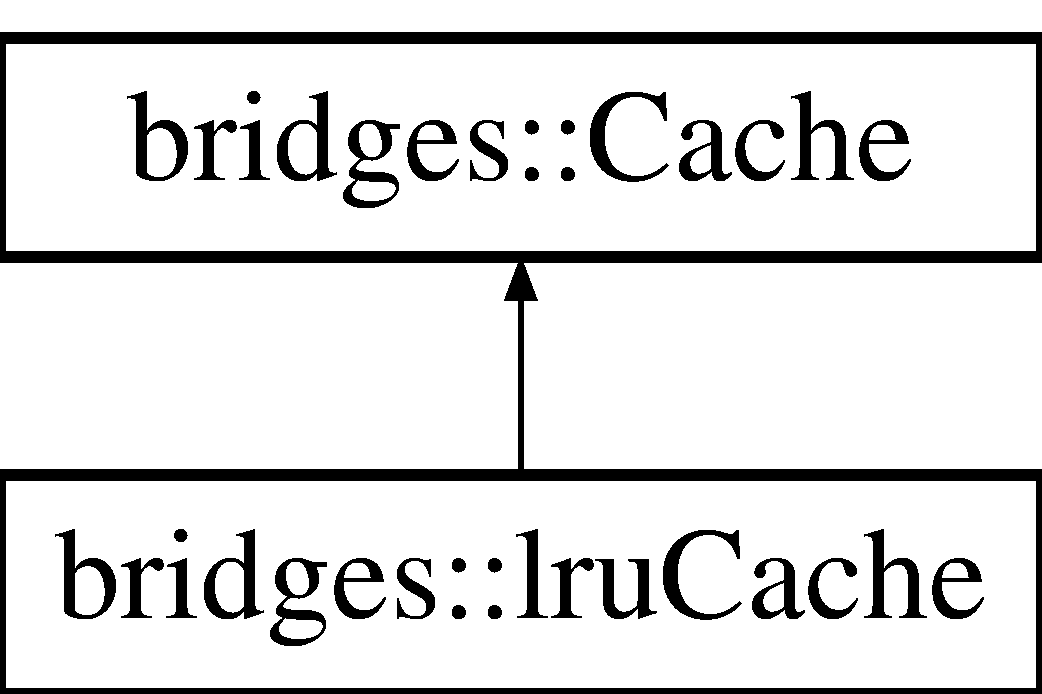
\includegraphics[height=2.000000cm]{classbridges_1_1lru_cache}
\end{center}
\end{figure}
\subsection*{Public Member Functions}
\begin{DoxyCompactItemize}
\item 
\hyperlink{classbridges_1_1lru_cache_ab21417b9fdc01613ec4ef3378c027593}{lru\+Cache} (int max\+File\+Number=30)
\item 
virtual std\+::string \hyperlink{classbridges_1_1lru_cache_ac8bed8ab7cbf002a23573c071ba04ad6}{get\+Doc} (const std\+::string \&hash\+\_\+value) override
\item 
virtual bool \hyperlink{classbridges_1_1lru_cache_ab56c75166ddcc3d17e6924e581f7a4e8}{in\+Cache} (const std\+::string \&hash\+\_\+value) override
\item 
virtual void \hyperlink{classbridges_1_1lru_cache_a927fa1186ba830717ce11898c2beb4c7}{put\+Doc} (const std\+::string \&hash\+\_\+value, const std\+::string \&content) override
\end{DoxyCompactItemize}


\subsection{Constructor \& Destructor Documentation}
\mbox{\Hypertarget{classbridges_1_1lru_cache_ab21417b9fdc01613ec4ef3378c027593}\label{classbridges_1_1lru_cache_ab21417b9fdc01613ec4ef3378c027593}} 
\index{bridges\+::lru\+Cache@{bridges\+::lru\+Cache}!lru\+Cache@{lru\+Cache}}
\index{lru\+Cache@{lru\+Cache}!bridges\+::lru\+Cache@{bridges\+::lru\+Cache}}
\subsubsection{\texorpdfstring{lru\+Cache()}{lruCache()}}
{\footnotesize\ttfamily bridges\+::lru\+Cache\+::lru\+Cache (\begin{DoxyParamCaption}\item[{int}]{max\+File\+Number = {\ttfamily 30} }\end{DoxyParamCaption})\hspace{0.3cm}{\ttfamily [inline]}}



\subsection{Member Function Documentation}
\mbox{\Hypertarget{classbridges_1_1lru_cache_ac8bed8ab7cbf002a23573c071ba04ad6}\label{classbridges_1_1lru_cache_ac8bed8ab7cbf002a23573c071ba04ad6}} 
\index{bridges\+::lru\+Cache@{bridges\+::lru\+Cache}!get\+Doc@{get\+Doc}}
\index{get\+Doc@{get\+Doc}!bridges\+::lru\+Cache@{bridges\+::lru\+Cache}}
\subsubsection{\texorpdfstring{get\+Doc()}{getDoc()}}
{\footnotesize\ttfamily virtual std\+::string bridges\+::lru\+Cache\+::get\+Doc (\begin{DoxyParamCaption}\item[{const std\+::string \&}]{hash\+\_\+value }\end{DoxyParamCaption})\hspace{0.3cm}{\ttfamily [inline]}, {\ttfamily [override]}, {\ttfamily [virtual]}}



Implements \hyperlink{classbridges_1_1_cache_abc1eaca36899e6e85df1c9a690f1d4dd}{bridges\+::\+Cache}.

\mbox{\Hypertarget{classbridges_1_1lru_cache_ab56c75166ddcc3d17e6924e581f7a4e8}\label{classbridges_1_1lru_cache_ab56c75166ddcc3d17e6924e581f7a4e8}} 
\index{bridges\+::lru\+Cache@{bridges\+::lru\+Cache}!in\+Cache@{in\+Cache}}
\index{in\+Cache@{in\+Cache}!bridges\+::lru\+Cache@{bridges\+::lru\+Cache}}
\subsubsection{\texorpdfstring{in\+Cache()}{inCache()}}
{\footnotesize\ttfamily virtual bool bridges\+::lru\+Cache\+::in\+Cache (\begin{DoxyParamCaption}\item[{const std\+::string \&}]{hash\+\_\+value }\end{DoxyParamCaption})\hspace{0.3cm}{\ttfamily [inline]}, {\ttfamily [override]}, {\ttfamily [virtual]}}



Implements \hyperlink{classbridges_1_1_cache_abf3601225841d14dcd5611cd6a223ba4}{bridges\+::\+Cache}.

\mbox{\Hypertarget{classbridges_1_1lru_cache_a927fa1186ba830717ce11898c2beb4c7}\label{classbridges_1_1lru_cache_a927fa1186ba830717ce11898c2beb4c7}} 
\index{bridges\+::lru\+Cache@{bridges\+::lru\+Cache}!put\+Doc@{put\+Doc}}
\index{put\+Doc@{put\+Doc}!bridges\+::lru\+Cache@{bridges\+::lru\+Cache}}
\subsubsection{\texorpdfstring{put\+Doc()}{putDoc()}}
{\footnotesize\ttfamily virtual void bridges\+::lru\+Cache\+::put\+Doc (\begin{DoxyParamCaption}\item[{const std\+::string \&}]{hash\+\_\+value,  }\item[{const std\+::string \&}]{content }\end{DoxyParamCaption})\hspace{0.3cm}{\ttfamily [inline]}, {\ttfamily [override]}, {\ttfamily [virtual]}}



Implements \hyperlink{classbridges_1_1_cache_ae74225542568a377fdcaf0354e466954}{bridges\+::\+Cache}.



The documentation for this class was generated from the following file\+:\begin{DoxyCompactItemize}
\item 
/home/erik/work/bridges/bridges-\/cxx/src/\hyperlink{_cache_8h}{Cache.\+h}\end{DoxyCompactItemize}

\hypertarget{classsio_1_1message}{}\section{sio\+:\+:message Class Reference}
\label{classsio_1_1message}\index{sio\+::message@{sio\+::message}}


{\ttfamily \#include $<$sio\+\_\+message.\+h$>$}

Inheritance diagram for sio\+:\+:message\+:\begin{figure}[H]
\begin{center}
\leavevmode
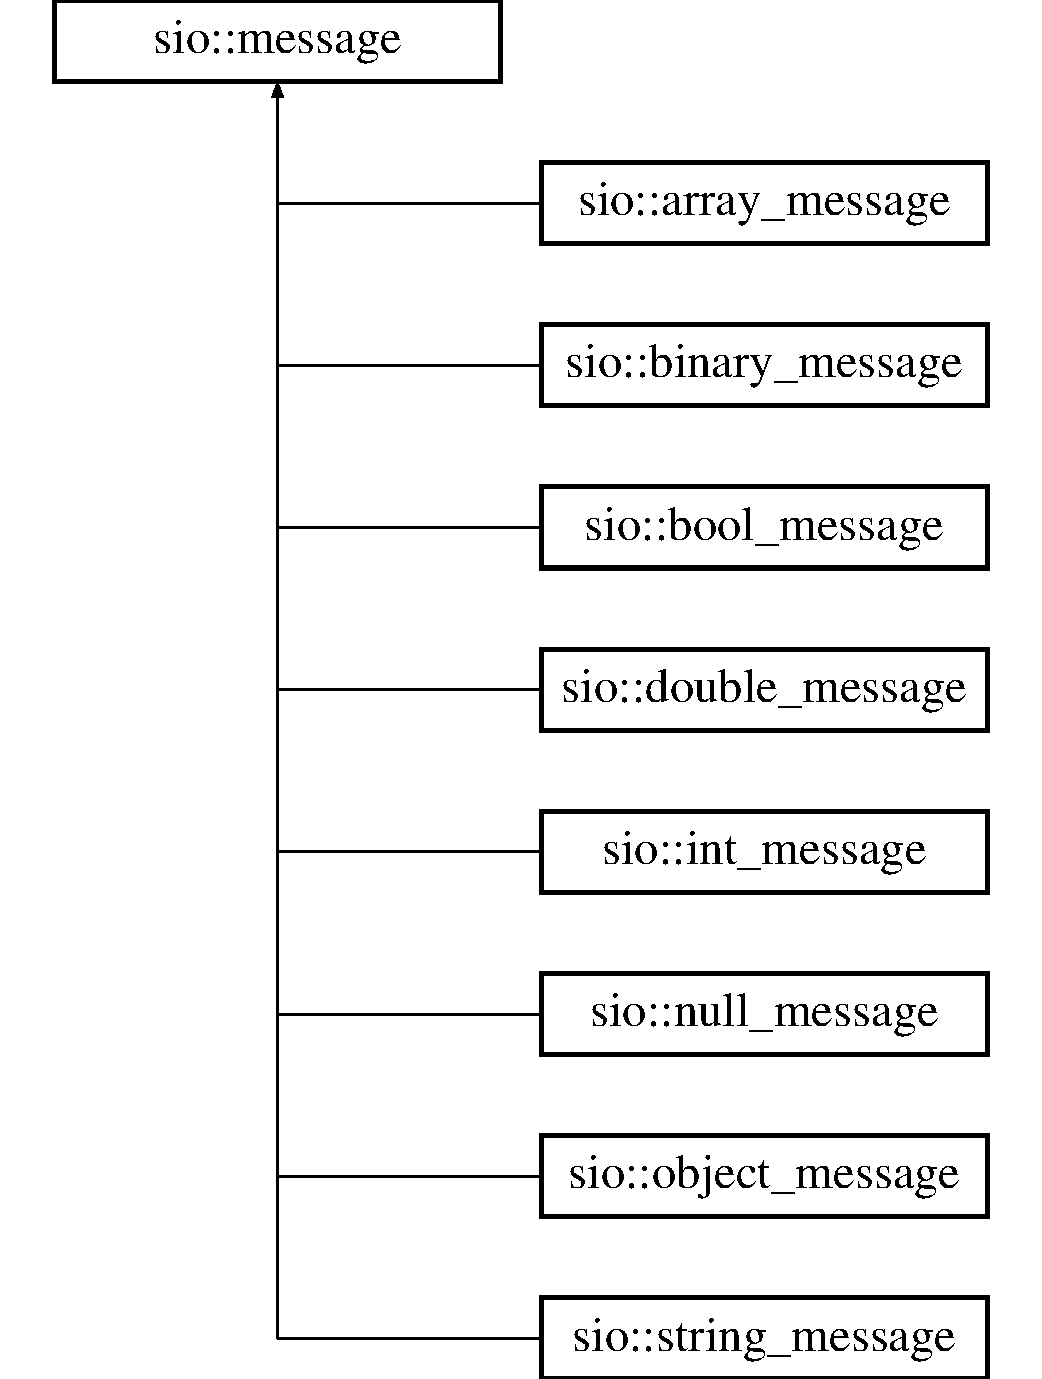
\includegraphics[height=9.000000cm]{classsio_1_1message}
\end{center}
\end{figure}
\subsection*{Classes}
\begin{DoxyCompactItemize}
\item 
class \hyperlink{classsio_1_1message_1_1list}{list}
\end{DoxyCompactItemize}
\subsection*{Public Types}
\begin{DoxyCompactItemize}
\item 
enum \hyperlink{classsio_1_1message_a5274f78a8f77cd535d4acf476badf769}{flag} \{ \newline
\hyperlink{classsio_1_1message_a5274f78a8f77cd535d4acf476badf769a6ffb67dfa74fef6da742b056a65871ae}{flag\+\_\+integer}, 
\hyperlink{classsio_1_1message_a5274f78a8f77cd535d4acf476badf769a5f4b2264d8c16031d3f3f43c2f246f0f}{flag\+\_\+double}, 
\hyperlink{classsio_1_1message_a5274f78a8f77cd535d4acf476badf769a25057139980e46d1a27cd184cf32e564}{flag\+\_\+string}, 
\hyperlink{classsio_1_1message_a5274f78a8f77cd535d4acf476badf769a004bcfc6977e87ae3752493f78180b72}{flag\+\_\+binary}, 
\newline
\hyperlink{classsio_1_1message_a5274f78a8f77cd535d4acf476badf769a4965ec8ed49a302baf6fb6f720ff10fb}{flag\+\_\+array}, 
\hyperlink{classsio_1_1message_a5274f78a8f77cd535d4acf476badf769a8707b49b4ab6d18bc8ec6c42379f217d}{flag\+\_\+object}, 
\hyperlink{classsio_1_1message_a5274f78a8f77cd535d4acf476badf769a97c7fce25aecaae75b690216a7ac2eb4}{flag\+\_\+boolean}, 
\hyperlink{classsio_1_1message_a5274f78a8f77cd535d4acf476badf769abf8e5572bf864afa7bc55ee3142a109e}{flag\+\_\+null}
 \}
\item 
typedef std\+::shared\+\_\+ptr$<$ \hyperlink{classsio_1_1message}{message} $>$ \hyperlink{classsio_1_1message_a6340b6fef57e4516eb17928b1885a615}{ptr}
\end{DoxyCompactItemize}
\subsection*{Public Member Functions}
\begin{DoxyCompactItemize}
\item 
virtual \hyperlink{classsio_1_1message_a0fe3f725f2cd8b207b43a9dbe24fe1c5}{$\sim$message} ()
\item 
\hyperlink{classsio_1_1message_a5274f78a8f77cd535d4acf476badf769}{flag} \hyperlink{classsio_1_1message_a2c8eb600ca29b420a5a1d826f0f6d5e6}{get\+\_\+flag} () const
\item 
virtual bool \hyperlink{classsio_1_1message_a3acbec589c3dc214d44dd4db1a6f8a2c}{get\+\_\+bool} () const
\item 
virtual int64\+\_\+t \hyperlink{classsio_1_1message_ae77c363200284d6741f0ac92f0e13ed2}{get\+\_\+int} () const
\item 
virtual double \hyperlink{classsio_1_1message_aa89963cd233b29653df1ce1943f9ea57}{get\+\_\+double} () const
\item 
virtual std\+::string const  \& \hyperlink{classsio_1_1message_a8e923d7e688e1bc69b586ef33684dd7a}{get\+\_\+string} () const
\item 
virtual std\+::shared\+\_\+ptr$<$ const std\+::string $>$ const  \& \hyperlink{classsio_1_1message_a55b9eeeb305f46bbf21ae339501174c2}{get\+\_\+binary} () const
\item 
virtual const std\+::vector$<$ \hyperlink{classsio_1_1message_a6340b6fef57e4516eb17928b1885a615}{ptr} $>$ \& \hyperlink{classsio_1_1message_af310192e16427f655dc89c627aae4fe7}{get\+\_\+vector} () const
\item 
virtual std\+::vector$<$ \hyperlink{classsio_1_1message_a6340b6fef57e4516eb17928b1885a615}{ptr} $>$ \& \hyperlink{classsio_1_1message_af62004da998c98ee7039a26d809c44d3}{get\+\_\+vector} ()
\item 
virtual const std\+::map$<$ std\+::string, \hyperlink{classsio_1_1message_a6340b6fef57e4516eb17928b1885a615}{message\+::ptr} $>$ \& \hyperlink{classsio_1_1message_a954a981a468fcea36ff19cce6ae7fd5e}{get\+\_\+map} () const
\item 
virtual std\+::map$<$ std\+::string, \hyperlink{classsio_1_1message_a6340b6fef57e4516eb17928b1885a615}{message\+::ptr} $>$ \& \hyperlink{classsio_1_1message_a6ca4aee4616aa9dfde4de317d5efd125}{get\+\_\+map} ()
\end{DoxyCompactItemize}
\subsection*{Protected Member Functions}
\begin{DoxyCompactItemize}
\item 
\hyperlink{classsio_1_1message_a592180d0792737b4bb73f5e5c30e386e}{message} (\hyperlink{classsio_1_1message_a5274f78a8f77cd535d4acf476badf769}{flag} f)
\end{DoxyCompactItemize}


\subsection{Member Typedef Documentation}
\mbox{\Hypertarget{classsio_1_1message_a6340b6fef57e4516eb17928b1885a615}\label{classsio_1_1message_a6340b6fef57e4516eb17928b1885a615}} 
\index{sio\+::message@{sio\+::message}!ptr@{ptr}}
\index{ptr@{ptr}!sio\+::message@{sio\+::message}}
\subsubsection{\texorpdfstring{ptr}{ptr}}
{\footnotesize\ttfamily typedef std\+::shared\+\_\+ptr$<$\hyperlink{classsio_1_1message}{message}$>$ \hyperlink{classsio_1_1message_a6340b6fef57e4516eb17928b1885a615}{sio\+::message\+::ptr}}



\subsection{Member Enumeration Documentation}
\mbox{\Hypertarget{classsio_1_1message_a5274f78a8f77cd535d4acf476badf769}\label{classsio_1_1message_a5274f78a8f77cd535d4acf476badf769}} 
\index{sio\+::message@{sio\+::message}!flag@{flag}}
\index{flag@{flag}!sio\+::message@{sio\+::message}}
\subsubsection{\texorpdfstring{flag}{flag}}
{\footnotesize\ttfamily enum \hyperlink{classsio_1_1message_a5274f78a8f77cd535d4acf476badf769}{sio\+::message\+::flag}}

\begin{DoxyEnumFields}{Enumerator}
\raisebox{\heightof{T}}[0pt][0pt]{\index{flag\+\_\+integer@{flag\+\_\+integer}!sio\+::message@{sio\+::message}}\index{sio\+::message@{sio\+::message}!flag\+\_\+integer@{flag\+\_\+integer}}}\mbox{\Hypertarget{classsio_1_1message_a5274f78a8f77cd535d4acf476badf769a6ffb67dfa74fef6da742b056a65871ae}\label{classsio_1_1message_a5274f78a8f77cd535d4acf476badf769a6ffb67dfa74fef6da742b056a65871ae}} 
flag\+\_\+integer&\\
\hline

\raisebox{\heightof{T}}[0pt][0pt]{\index{flag\+\_\+double@{flag\+\_\+double}!sio\+::message@{sio\+::message}}\index{sio\+::message@{sio\+::message}!flag\+\_\+double@{flag\+\_\+double}}}\mbox{\Hypertarget{classsio_1_1message_a5274f78a8f77cd535d4acf476badf769a5f4b2264d8c16031d3f3f43c2f246f0f}\label{classsio_1_1message_a5274f78a8f77cd535d4acf476badf769a5f4b2264d8c16031d3f3f43c2f246f0f}} 
flag\+\_\+double&\\
\hline

\raisebox{\heightof{T}}[0pt][0pt]{\index{flag\+\_\+string@{flag\+\_\+string}!sio\+::message@{sio\+::message}}\index{sio\+::message@{sio\+::message}!flag\+\_\+string@{flag\+\_\+string}}}\mbox{\Hypertarget{classsio_1_1message_a5274f78a8f77cd535d4acf476badf769a25057139980e46d1a27cd184cf32e564}\label{classsio_1_1message_a5274f78a8f77cd535d4acf476badf769a25057139980e46d1a27cd184cf32e564}} 
flag\+\_\+string&\\
\hline

\raisebox{\heightof{T}}[0pt][0pt]{\index{flag\+\_\+binary@{flag\+\_\+binary}!sio\+::message@{sio\+::message}}\index{sio\+::message@{sio\+::message}!flag\+\_\+binary@{flag\+\_\+binary}}}\mbox{\Hypertarget{classsio_1_1message_a5274f78a8f77cd535d4acf476badf769a004bcfc6977e87ae3752493f78180b72}\label{classsio_1_1message_a5274f78a8f77cd535d4acf476badf769a004bcfc6977e87ae3752493f78180b72}} 
flag\+\_\+binary&\\
\hline

\raisebox{\heightof{T}}[0pt][0pt]{\index{flag\+\_\+array@{flag\+\_\+array}!sio\+::message@{sio\+::message}}\index{sio\+::message@{sio\+::message}!flag\+\_\+array@{flag\+\_\+array}}}\mbox{\Hypertarget{classsio_1_1message_a5274f78a8f77cd535d4acf476badf769a4965ec8ed49a302baf6fb6f720ff10fb}\label{classsio_1_1message_a5274f78a8f77cd535d4acf476badf769a4965ec8ed49a302baf6fb6f720ff10fb}} 
flag\+\_\+array&\\
\hline

\raisebox{\heightof{T}}[0pt][0pt]{\index{flag\+\_\+object@{flag\+\_\+object}!sio\+::message@{sio\+::message}}\index{sio\+::message@{sio\+::message}!flag\+\_\+object@{flag\+\_\+object}}}\mbox{\Hypertarget{classsio_1_1message_a5274f78a8f77cd535d4acf476badf769a8707b49b4ab6d18bc8ec6c42379f217d}\label{classsio_1_1message_a5274f78a8f77cd535d4acf476badf769a8707b49b4ab6d18bc8ec6c42379f217d}} 
flag\+\_\+object&\\
\hline

\raisebox{\heightof{T}}[0pt][0pt]{\index{flag\+\_\+boolean@{flag\+\_\+boolean}!sio\+::message@{sio\+::message}}\index{sio\+::message@{sio\+::message}!flag\+\_\+boolean@{flag\+\_\+boolean}}}\mbox{\Hypertarget{classsio_1_1message_a5274f78a8f77cd535d4acf476badf769a97c7fce25aecaae75b690216a7ac2eb4}\label{classsio_1_1message_a5274f78a8f77cd535d4acf476badf769a97c7fce25aecaae75b690216a7ac2eb4}} 
flag\+\_\+boolean&\\
\hline

\raisebox{\heightof{T}}[0pt][0pt]{\index{flag\+\_\+null@{flag\+\_\+null}!sio\+::message@{sio\+::message}}\index{sio\+::message@{sio\+::message}!flag\+\_\+null@{flag\+\_\+null}}}\mbox{\Hypertarget{classsio_1_1message_a5274f78a8f77cd535d4acf476badf769abf8e5572bf864afa7bc55ee3142a109e}\label{classsio_1_1message_a5274f78a8f77cd535d4acf476badf769abf8e5572bf864afa7bc55ee3142a109e}} 
flag\+\_\+null&\\
\hline

\end{DoxyEnumFields}


\subsection{Constructor \& Destructor Documentation}
\mbox{\Hypertarget{classsio_1_1message_a0fe3f725f2cd8b207b43a9dbe24fe1c5}\label{classsio_1_1message_a0fe3f725f2cd8b207b43a9dbe24fe1c5}} 
\index{sio\+::message@{sio\+::message}!````~message@{$\sim$message}}
\index{````~message@{$\sim$message}!sio\+::message@{sio\+::message}}
\subsubsection{\texorpdfstring{$\sim$message()}{~message()}}
{\footnotesize\ttfamily virtual sio\+::message\+::$\sim$message (\begin{DoxyParamCaption}{ }\end{DoxyParamCaption})\hspace{0.3cm}{\ttfamily [inline]}, {\ttfamily [virtual]}}

\mbox{\Hypertarget{classsio_1_1message_a592180d0792737b4bb73f5e5c30e386e}\label{classsio_1_1message_a592180d0792737b4bb73f5e5c30e386e}} 
\index{sio\+::message@{sio\+::message}!message@{message}}
\index{message@{message}!sio\+::message@{sio\+::message}}
\subsubsection{\texorpdfstring{message()}{message()}}
{\footnotesize\ttfamily sio\+::message\+::message (\begin{DoxyParamCaption}\item[{\hyperlink{classsio_1_1message_a5274f78a8f77cd535d4acf476badf769}{flag}}]{f }\end{DoxyParamCaption})\hspace{0.3cm}{\ttfamily [inline]}, {\ttfamily [protected]}}



\subsection{Member Function Documentation}
\mbox{\Hypertarget{classsio_1_1message_a55b9eeeb305f46bbf21ae339501174c2}\label{classsio_1_1message_a55b9eeeb305f46bbf21ae339501174c2}} 
\index{sio\+::message@{sio\+::message}!get\+\_\+binary@{get\+\_\+binary}}
\index{get\+\_\+binary@{get\+\_\+binary}!sio\+::message@{sio\+::message}}
\subsubsection{\texorpdfstring{get\+\_\+binary()}{get\_binary()}}
{\footnotesize\ttfamily virtual std\+::shared\+\_\+ptr$<$const std\+::string$>$ const\& sio\+::message\+::get\+\_\+binary (\begin{DoxyParamCaption}{ }\end{DoxyParamCaption}) const\hspace{0.3cm}{\ttfamily [inline]}, {\ttfamily [virtual]}}



Reimplemented in \hyperlink{classsio_1_1binary__message_aac4db910fd9afb507ef0750394c5cd29}{sio\+::binary\+\_\+message}.

\mbox{\Hypertarget{classsio_1_1message_a3acbec589c3dc214d44dd4db1a6f8a2c}\label{classsio_1_1message_a3acbec589c3dc214d44dd4db1a6f8a2c}} 
\index{sio\+::message@{sio\+::message}!get\+\_\+bool@{get\+\_\+bool}}
\index{get\+\_\+bool@{get\+\_\+bool}!sio\+::message@{sio\+::message}}
\subsubsection{\texorpdfstring{get\+\_\+bool()}{get\_bool()}}
{\footnotesize\ttfamily virtual bool sio\+::message\+::get\+\_\+bool (\begin{DoxyParamCaption}{ }\end{DoxyParamCaption}) const\hspace{0.3cm}{\ttfamily [inline]}, {\ttfamily [virtual]}}



Reimplemented in \hyperlink{classsio_1_1bool__message_aca66ff64b5ac4198c5292e26abdf9e92}{sio\+::bool\+\_\+message}.

\mbox{\Hypertarget{classsio_1_1message_aa89963cd233b29653df1ce1943f9ea57}\label{classsio_1_1message_aa89963cd233b29653df1ce1943f9ea57}} 
\index{sio\+::message@{sio\+::message}!get\+\_\+double@{get\+\_\+double}}
\index{get\+\_\+double@{get\+\_\+double}!sio\+::message@{sio\+::message}}
\subsubsection{\texorpdfstring{get\+\_\+double()}{get\_double()}}
{\footnotesize\ttfamily virtual double sio\+::message\+::get\+\_\+double (\begin{DoxyParamCaption}{ }\end{DoxyParamCaption}) const\hspace{0.3cm}{\ttfamily [inline]}, {\ttfamily [virtual]}}



Reimplemented in \hyperlink{classsio_1_1double__message_a0ab6e4c4e579356b367bb0ef37e79c62}{sio\+::double\+\_\+message}, and \hyperlink{classsio_1_1int__message_a7fdc141b0fe04ce1b75054b6de110f2c}{sio\+::int\+\_\+message}.

\mbox{\Hypertarget{classsio_1_1message_a2c8eb600ca29b420a5a1d826f0f6d5e6}\label{classsio_1_1message_a2c8eb600ca29b420a5a1d826f0f6d5e6}} 
\index{sio\+::message@{sio\+::message}!get\+\_\+flag@{get\+\_\+flag}}
\index{get\+\_\+flag@{get\+\_\+flag}!sio\+::message@{sio\+::message}}
\subsubsection{\texorpdfstring{get\+\_\+flag()}{get\_flag()}}
{\footnotesize\ttfamily \hyperlink{classsio_1_1message_a5274f78a8f77cd535d4acf476badf769}{flag} sio\+::message\+::get\+\_\+flag (\begin{DoxyParamCaption}{ }\end{DoxyParamCaption}) const\hspace{0.3cm}{\ttfamily [inline]}}

\mbox{\Hypertarget{classsio_1_1message_ae77c363200284d6741f0ac92f0e13ed2}\label{classsio_1_1message_ae77c363200284d6741f0ac92f0e13ed2}} 
\index{sio\+::message@{sio\+::message}!get\+\_\+int@{get\+\_\+int}}
\index{get\+\_\+int@{get\+\_\+int}!sio\+::message@{sio\+::message}}
\subsubsection{\texorpdfstring{get\+\_\+int()}{get\_int()}}
{\footnotesize\ttfamily virtual int64\+\_\+t sio\+::message\+::get\+\_\+int (\begin{DoxyParamCaption}{ }\end{DoxyParamCaption}) const\hspace{0.3cm}{\ttfamily [inline]}, {\ttfamily [virtual]}}



Reimplemented in \hyperlink{classsio_1_1int__message_ad9159e1285bd3efd15b8f87699a9b133}{sio\+::int\+\_\+message}.

\mbox{\Hypertarget{classsio_1_1message_a954a981a468fcea36ff19cce6ae7fd5e}\label{classsio_1_1message_a954a981a468fcea36ff19cce6ae7fd5e}} 
\index{sio\+::message@{sio\+::message}!get\+\_\+map@{get\+\_\+map}}
\index{get\+\_\+map@{get\+\_\+map}!sio\+::message@{sio\+::message}}
\subsubsection{\texorpdfstring{get\+\_\+map()}{get\_map()}\hspace{0.1cm}{\footnotesize\ttfamily [1/2]}}
{\footnotesize\ttfamily virtual const std\+::map$<$std\+::string, \hyperlink{classsio_1_1message_a6340b6fef57e4516eb17928b1885a615}{message\+::ptr}$>$\& sio\+::message\+::get\+\_\+map (\begin{DoxyParamCaption}{ }\end{DoxyParamCaption}) const\hspace{0.3cm}{\ttfamily [inline]}, {\ttfamily [virtual]}}



Reimplemented in \hyperlink{classsio_1_1object__message_a35d7f1d654b2a3b753ac01444635203e}{sio\+::object\+\_\+message}.

\mbox{\Hypertarget{classsio_1_1message_a6ca4aee4616aa9dfde4de317d5efd125}\label{classsio_1_1message_a6ca4aee4616aa9dfde4de317d5efd125}} 
\index{sio\+::message@{sio\+::message}!get\+\_\+map@{get\+\_\+map}}
\index{get\+\_\+map@{get\+\_\+map}!sio\+::message@{sio\+::message}}
\subsubsection{\texorpdfstring{get\+\_\+map()}{get\_map()}\hspace{0.1cm}{\footnotesize\ttfamily [2/2]}}
{\footnotesize\ttfamily virtual std\+::map$<$std\+::string, \hyperlink{classsio_1_1message_a6340b6fef57e4516eb17928b1885a615}{message\+::ptr}$>$\& sio\+::message\+::get\+\_\+map (\begin{DoxyParamCaption}{ }\end{DoxyParamCaption})\hspace{0.3cm}{\ttfamily [inline]}, {\ttfamily [virtual]}}



Reimplemented in \hyperlink{classsio_1_1object__message_ac024fab0eb24248150ab318a4b937b4e}{sio\+::object\+\_\+message}.

\mbox{\Hypertarget{classsio_1_1message_a8e923d7e688e1bc69b586ef33684dd7a}\label{classsio_1_1message_a8e923d7e688e1bc69b586ef33684dd7a}} 
\index{sio\+::message@{sio\+::message}!get\+\_\+string@{get\+\_\+string}}
\index{get\+\_\+string@{get\+\_\+string}!sio\+::message@{sio\+::message}}
\subsubsection{\texorpdfstring{get\+\_\+string()}{get\_string()}}
{\footnotesize\ttfamily virtual std\+::string const\& sio\+::message\+::get\+\_\+string (\begin{DoxyParamCaption}{ }\end{DoxyParamCaption}) const\hspace{0.3cm}{\ttfamily [inline]}, {\ttfamily [virtual]}}



Reimplemented in \hyperlink{classsio_1_1string__message_a8c79f0c15468e15251029c9f1612ca44}{sio\+::string\+\_\+message}.

\mbox{\Hypertarget{classsio_1_1message_af310192e16427f655dc89c627aae4fe7}\label{classsio_1_1message_af310192e16427f655dc89c627aae4fe7}} 
\index{sio\+::message@{sio\+::message}!get\+\_\+vector@{get\+\_\+vector}}
\index{get\+\_\+vector@{get\+\_\+vector}!sio\+::message@{sio\+::message}}
\subsubsection{\texorpdfstring{get\+\_\+vector()}{get\_vector()}\hspace{0.1cm}{\footnotesize\ttfamily [1/2]}}
{\footnotesize\ttfamily virtual const std\+::vector$<$\hyperlink{classsio_1_1message_a6340b6fef57e4516eb17928b1885a615}{ptr}$>$\& sio\+::message\+::get\+\_\+vector (\begin{DoxyParamCaption}{ }\end{DoxyParamCaption}) const\hspace{0.3cm}{\ttfamily [inline]}, {\ttfamily [virtual]}}



Reimplemented in \hyperlink{classsio_1_1array__message_a298e6b4d041e95ac5b90cdff6fdef5fb}{sio\+::array\+\_\+message}.

\mbox{\Hypertarget{classsio_1_1message_af62004da998c98ee7039a26d809c44d3}\label{classsio_1_1message_af62004da998c98ee7039a26d809c44d3}} 
\index{sio\+::message@{sio\+::message}!get\+\_\+vector@{get\+\_\+vector}}
\index{get\+\_\+vector@{get\+\_\+vector}!sio\+::message@{sio\+::message}}
\subsubsection{\texorpdfstring{get\+\_\+vector()}{get\_vector()}\hspace{0.1cm}{\footnotesize\ttfamily [2/2]}}
{\footnotesize\ttfamily virtual std\+::vector$<$\hyperlink{classsio_1_1message_a6340b6fef57e4516eb17928b1885a615}{ptr}$>$\& sio\+::message\+::get\+\_\+vector (\begin{DoxyParamCaption}{ }\end{DoxyParamCaption})\hspace{0.3cm}{\ttfamily [inline]}, {\ttfamily [virtual]}}



Reimplemented in \hyperlink{classsio_1_1array__message_a7d039c4e78bb01f5e19921e0f09509c2}{sio\+::array\+\_\+message}.



The documentation for this class was generated from the following file\+:\begin{DoxyCompactItemize}
\item 
/home/erik/work/bridges/bridges-\/cxx/src/\hyperlink{sio__message_8h}{sio\+\_\+message.\+h}\end{DoxyCompactItemize}

\hypertarget{classbridges_1_1datastructure_1_1_m_lelement}{}\doxysection{bridges\+::datastructure\+::MLelement$<$ E $>$ Class Template Reference}
\label{classbridges_1_1datastructure_1_1_m_lelement}\index{bridges::datastructure::MLelement$<$ E $>$@{bridges::datastructure::MLelement$<$ E $>$}}


{\ttfamily \#include $<$MLelement.\+h$>$}

Inheritance diagram for bridges\+::datastructure\+::MLelement$<$ E $>$\+:\begin{figure}[H]
\begin{center}
\leavevmode
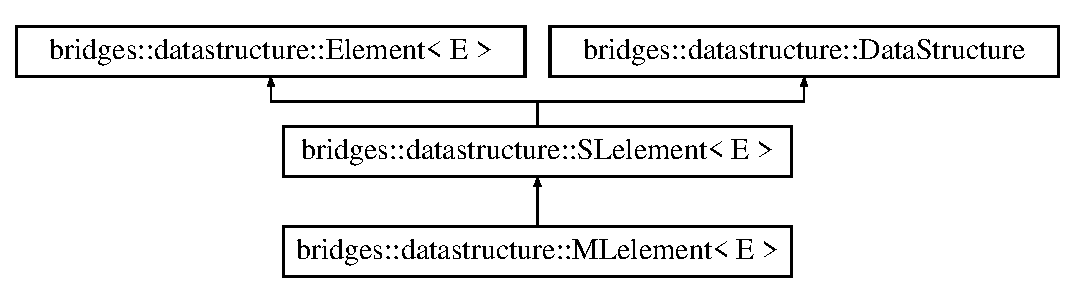
\includegraphics[height=3.000000cm]{classbridges_1_1datastructure_1_1_m_lelement}
\end{center}
\end{figure}


\doxysubsection{Detailed Description}
\subsubsection*{template$<$typename E$>$\newline
class bridges\+::datastructure\+::\+MLelement$<$ E $>$}

This class can be used to instantiate Multi-\/list Elements. 

This class extends \mbox{\hyperlink{classbridges_1_1datastructure_1_1_s_lelement}{SLelement}} (singly linked list element) to build multi-\/lists; Multilist elements contain a tag (boolean) that indicates if the element contains a sublist or not; if the tag is true, then there is a sublist beginning at this node and the starting point is the `sublist' field in the element. If the tag is false, then the list continues as a normal singly linked list. The sublists are re recursive\+: any sublist can have its own sublists and so on. As in singly linked elements, the next pointer points to the following list element and each element contains a generic application specific object.

Multi-\/list elements contain a visualizer (\mbox{\hyperlink{classbridges_1_1datastructure_1_1_element_visualizer}{Element\+Visualizer}}) object for setting visual attributes (color, shape, opacity, size), necessary for displaying them in a web browser.

Elements also have a \mbox{\hyperlink{classbridges_1_1datastructure_1_1_link_visualizer}{Link\+Visualizer}} object, that is used when they are linked to another element, appropriate for setting link attributes, for instance, between the current element and its next element. In this case, the link in question is that which connects the element to the following elements; a similar logic follows for sublists.

\begin{DoxySeeAlso}{See also}
There is a tutorial about Multi Lists \+: \href{https://bridgesuncc.github.io/tutorials/MultiList.html}{\texttt{ https\+://bridgesuncc.\+github.\+io/tutorials/\+Multi\+List.\+html}}
\end{DoxySeeAlso}
\begin{DoxyAuthor}{Author}
Kalpathi Subramanian
\end{DoxyAuthor}
\begin{DoxyDate}{Date}
5/24/17, 7/12/19, 12/28/20
\end{DoxyDate}

\begin{DoxyParams}{Parameters}
{\em E} & The generic parameter object that is part of this element, representing either application specific data, or a pointer to a sublist. \\
\hline
\end{DoxyParams}
\doxysubsection*{Public Member Functions}
\begin{DoxyCompactItemize}
\item 
\mbox{\hyperlink{classbridges_1_1datastructure_1_1_m_lelement_af73050e460a47d0b5d82ee6ae49b6c59}{MLelement}} (const E \&val=E(), const string \&lab=string())
\begin{DoxyCompactList}\small\item\em constructor \end{DoxyCompactList}\item 
\mbox{\hyperlink{classbridges_1_1datastructure_1_1_m_lelement_aae22c04d644bcab2eba56bb8dc84d5eb}{MLelement}} (string label)
\begin{DoxyCompactList}\small\item\em Creates an \mbox{\hyperlink{classbridges_1_1datastructure_1_1_m_lelement}{MLelement}} object. \end{DoxyCompactList}\item 
\mbox{\hyperlink{classbridges_1_1datastructure_1_1_m_lelement_ac3349ecdbce79646839cdb9ea1e90b2f}{MLelement}} (E e, \mbox{\hyperlink{classbridges_1_1datastructure_1_1_m_lelement}{MLelement}}$<$ E $>$ $\ast$\mbox{\hyperlink{classbridges_1_1datastructure_1_1_s_lelement_afc016a593a4a5aba82021ee34edadbfc}{next}})
\begin{DoxyCompactList}\small\item\em Creates an \mbox{\hyperlink{classbridges_1_1datastructure_1_1_m_lelement}{MLelement}} object. \end{DoxyCompactList}\item 
void \mbox{\hyperlink{classbridges_1_1datastructure_1_1_m_lelement_a5d6a2fa775c819c8c7609b539c93fe9f}{set\+Sub\+List}} (\mbox{\hyperlink{classbridges_1_1datastructure_1_1_m_lelement}{MLelement}}$<$ E $>$ $\ast$sl)
\begin{DoxyCompactList}\small\item\em Sets the start of a new sublist to the \mbox{\hyperlink{classbridges_1_1datastructure_1_1_m_lelement}{MLelement}} \char`\"{}next\char`\"{}. \end{DoxyCompactList}\item 
\mbox{\hyperlink{classbridges_1_1datastructure_1_1_m_lelement}{MLelement}} $\ast$ \mbox{\hyperlink{classbridges_1_1datastructure_1_1_m_lelement_a9faeb30ffd023746ce36e05705a62b2d}{get\+Sub\+List}} ()
\begin{DoxyCompactList}\small\item\em Gets the sublist at this node, if it exists. \end{DoxyCompactList}\item 
\mbox{\hyperlink{classbridges_1_1datastructure_1_1_m_lelement}{MLelement}}$<$ E $>$ $\ast$ \mbox{\hyperlink{classbridges_1_1datastructure_1_1_m_lelement_a47b417db0b948b6899eece572bef9274}{get\+Next}} () override
\begin{DoxyCompactList}\small\item\em Retrieves the element following this element. \end{DoxyCompactList}\item 
\mbox{\hyperlink{classbridges_1_1datastructure_1_1_m_lelement}{MLelement}}$<$ E $>$ $\ast$ \mbox{\hyperlink{classbridges_1_1datastructure_1_1_m_lelement_a611b3e7d54fdfbc622004a50ca718e6e}{get\+Next}} () const override
\begin{DoxyCompactList}\small\item\em Retrieves the element following this element -\/ const version. \end{DoxyCompactList}\item 
void \mbox{\hyperlink{classbridges_1_1datastructure_1_1_m_lelement_a13dfba9b3fa1af26c6d344fa7a086429}{set\+Next}} (\mbox{\hyperlink{classbridges_1_1datastructure_1_1_m_lelement}{MLelement}}$<$ E $>$ $\ast$n)
\begin{DoxyCompactList}\small\item\em Sets the element to point to the next \mbox{\hyperlink{classbridges_1_1datastructure_1_1_m_lelement}{MLelement}}. \end{DoxyCompactList}\item 
void \mbox{\hyperlink{classbridges_1_1datastructure_1_1_m_lelement_a32ba4ec57e6f5e1e65f82784a7f45804}{set\+Tag}} (bool t)
\begin{DoxyCompactList}\small\item\em Sets the tag of the element. \end{DoxyCompactList}\item 
bool \mbox{\hyperlink{classbridges_1_1datastructure_1_1_m_lelement_a44ef87048b6b0424478f498cf99149f2}{get\+Tag}} ()
\begin{DoxyCompactList}\small\item\em Gets the tag of the element. \end{DoxyCompactList}\item 
virtual const string \mbox{\hyperlink{classbridges_1_1datastructure_1_1_m_lelement_a735c3cb43648b4d4e7d3316cdc1a1952}{get\+DStype}} () const override
\begin{DoxyCompactList}\small\item\em Return the string representaion of element. \end{DoxyCompactList}\end{DoxyCompactItemize}
\doxysubsection*{Protected Attributes}
\begin{DoxyCompactItemize}
\item 
\mbox{\hyperlink{classbridges_1_1datastructure_1_1_m_lelement}{MLelement}}$<$ E $>$ $\ast$ \mbox{\hyperlink{classbridges_1_1datastructure_1_1_m_lelement_afe31ff363c0861efb8eacc12f2a651df}{sub\+\_\+list}} = nullptr
\item 
bool \mbox{\hyperlink{classbridges_1_1datastructure_1_1_m_lelement_aef061a364a85ebb0c0f2cdaff8c726e6}{tag}} = false
\end{DoxyCompactItemize}
\doxysubsection*{Additional Inherited Members}


\doxysubsection{Constructor \& Destructor Documentation}
\mbox{\Hypertarget{classbridges_1_1datastructure_1_1_m_lelement_af73050e460a47d0b5d82ee6ae49b6c59}\label{classbridges_1_1datastructure_1_1_m_lelement_af73050e460a47d0b5d82ee6ae49b6c59}} 
\index{bridges::datastructure::MLelement$<$ E $>$@{bridges::datastructure::MLelement$<$ E $>$}!MLelement@{MLelement}}
\index{MLelement@{MLelement}!bridges::datastructure::MLelement$<$ E $>$@{bridges::datastructure::MLelement$<$ E $>$}}
\doxysubsubsection{\texorpdfstring{MLelement()}{MLelement()}\hspace{0.1cm}{\footnotesize\ttfamily [1/3]}}
{\footnotesize\ttfamily template$<$typename E $>$ \\
\mbox{\hyperlink{classbridges_1_1datastructure_1_1_m_lelement}{bridges\+::datastructure\+::\+MLelement}}$<$ E $>$\+::\mbox{\hyperlink{classbridges_1_1datastructure_1_1_m_lelement}{MLelement}} (\begin{DoxyParamCaption}\item[{const E \&}]{val = {\ttfamily E()},  }\item[{const string \&}]{lab = {\ttfamily string()} }\end{DoxyParamCaption})\hspace{0.3cm}{\ttfamily [inline]}}



constructor 

This constructor creates an \mbox{\hyperlink{classbridges_1_1datastructure_1_1_m_lelement}{MLelement}} object and sets the next pointer to null


\begin{DoxyParams}{Parameters}
{\em val} & generic object \\
\hline
{\em lab} & label \\
\hline
\end{DoxyParams}
\mbox{\Hypertarget{classbridges_1_1datastructure_1_1_m_lelement_aae22c04d644bcab2eba56bb8dc84d5eb}\label{classbridges_1_1datastructure_1_1_m_lelement_aae22c04d644bcab2eba56bb8dc84d5eb}} 
\index{bridges::datastructure::MLelement$<$ E $>$@{bridges::datastructure::MLelement$<$ E $>$}!MLelement@{MLelement}}
\index{MLelement@{MLelement}!bridges::datastructure::MLelement$<$ E $>$@{bridges::datastructure::MLelement$<$ E $>$}}
\doxysubsubsection{\texorpdfstring{MLelement()}{MLelement()}\hspace{0.1cm}{\footnotesize\ttfamily [2/3]}}
{\footnotesize\ttfamily template$<$typename E $>$ \\
\mbox{\hyperlink{classbridges_1_1datastructure_1_1_m_lelement}{bridges\+::datastructure\+::\+MLelement}}$<$ E $>$\+::\mbox{\hyperlink{classbridges_1_1datastructure_1_1_m_lelement}{MLelement}} (\begin{DoxyParamCaption}\item[{string}]{label }\end{DoxyParamCaption})\hspace{0.3cm}{\ttfamily [inline]}}



Creates an \mbox{\hyperlink{classbridges_1_1datastructure_1_1_m_lelement}{MLelement}} object. 

This constructor creates an \mbox{\hyperlink{classbridges_1_1datastructure_1_1_m_lelement}{MLelement}} object of generic parameter object E, and label \char`\"{}label\char`\"{} and sets the next pointer to null


\begin{DoxyParams}{Parameters}
{\em label} & the label of \mbox{\hyperlink{classbridges_1_1datastructure_1_1_m_lelement}{MLelement}} that shows up on the \mbox{\hyperlink{classbridges_1_1_bridges}{Bridges}} visualization \\
\hline
\end{DoxyParams}
\mbox{\Hypertarget{classbridges_1_1datastructure_1_1_m_lelement_ac3349ecdbce79646839cdb9ea1e90b2f}\label{classbridges_1_1datastructure_1_1_m_lelement_ac3349ecdbce79646839cdb9ea1e90b2f}} 
\index{bridges::datastructure::MLelement$<$ E $>$@{bridges::datastructure::MLelement$<$ E $>$}!MLelement@{MLelement}}
\index{MLelement@{MLelement}!bridges::datastructure::MLelement$<$ E $>$@{bridges::datastructure::MLelement$<$ E $>$}}
\doxysubsubsection{\texorpdfstring{MLelement()}{MLelement()}\hspace{0.1cm}{\footnotesize\ttfamily [3/3]}}
{\footnotesize\ttfamily template$<$typename E $>$ \\
\mbox{\hyperlink{classbridges_1_1datastructure_1_1_m_lelement}{bridges\+::datastructure\+::\+MLelement}}$<$ E $>$\+::\mbox{\hyperlink{classbridges_1_1datastructure_1_1_m_lelement}{MLelement}} (\begin{DoxyParamCaption}\item[{E}]{e,  }\item[{\mbox{\hyperlink{classbridges_1_1datastructure_1_1_m_lelement}{MLelement}}$<$ E $>$ $\ast$}]{next }\end{DoxyParamCaption})\hspace{0.3cm}{\ttfamily [inline]}}



Creates an \mbox{\hyperlink{classbridges_1_1datastructure_1_1_m_lelement}{MLelement}} object. 

Creates a new element with value \char`\"{}e\char`\"{} and sets the next pointer to the \mbox{\hyperlink{classbridges_1_1datastructure_1_1_m_lelement}{MLelement}} referenced by the \char`\"{}next\char`\"{} argument


\begin{DoxyParams}{Parameters}
{\em e} & the generic object that this element will hold \\
\hline
{\em next} & the element that should be assigned to the next pointer \\
\hline
\end{DoxyParams}


\doxysubsection{Member Function Documentation}
\mbox{\Hypertarget{classbridges_1_1datastructure_1_1_m_lelement_a735c3cb43648b4d4e7d3316cdc1a1952}\label{classbridges_1_1datastructure_1_1_m_lelement_a735c3cb43648b4d4e7d3316cdc1a1952}} 
\index{bridges::datastructure::MLelement$<$ E $>$@{bridges::datastructure::MLelement$<$ E $>$}!getDStype@{getDStype}}
\index{getDStype@{getDStype}!bridges::datastructure::MLelement$<$ E $>$@{bridges::datastructure::MLelement$<$ E $>$}}
\doxysubsubsection{\texorpdfstring{getDStype()}{getDStype()}}
{\footnotesize\ttfamily template$<$typename E $>$ \\
virtual const string \mbox{\hyperlink{classbridges_1_1datastructure_1_1_m_lelement}{bridges\+::datastructure\+::\+MLelement}}$<$ E $>$\+::get\+DStype (\begin{DoxyParamCaption}{ }\end{DoxyParamCaption}) const\hspace{0.3cm}{\ttfamily [inline]}, {\ttfamily [override]}, {\ttfamily [virtual]}}



Return the string representaion of element. 

\begin{DoxyReturn}{Returns}
The string representation of this data structure type 
\end{DoxyReturn}


Reimplemented from \mbox{\hyperlink{classbridges_1_1datastructure_1_1_s_lelement_a602156aacacd73d1faa365d68d8af31b}{bridges\+::datastructure\+::\+SLelement$<$ E $>$}}.

\mbox{\Hypertarget{classbridges_1_1datastructure_1_1_m_lelement_a611b3e7d54fdfbc622004a50ca718e6e}\label{classbridges_1_1datastructure_1_1_m_lelement_a611b3e7d54fdfbc622004a50ca718e6e}} 
\index{bridges::datastructure::MLelement$<$ E $>$@{bridges::datastructure::MLelement$<$ E $>$}!getNext@{getNext}}
\index{getNext@{getNext}!bridges::datastructure::MLelement$<$ E $>$@{bridges::datastructure::MLelement$<$ E $>$}}
\doxysubsubsection{\texorpdfstring{getNext()}{getNext()}\hspace{0.1cm}{\footnotesize\ttfamily [1/2]}}
{\footnotesize\ttfamily template$<$typename E $>$ \\
\mbox{\hyperlink{classbridges_1_1datastructure_1_1_m_lelement}{MLelement}}$<$E$>$$\ast$ \mbox{\hyperlink{classbridges_1_1datastructure_1_1_m_lelement}{bridges\+::datastructure\+::\+MLelement}}$<$ E $>$\+::get\+Next (\begin{DoxyParamCaption}{ }\end{DoxyParamCaption}) const\hspace{0.3cm}{\ttfamily [inline]}, {\ttfamily [override]}, {\ttfamily [virtual]}}



Retrieves the element following this element -\/ const version. 

\begin{DoxyReturn}{Returns}
MLelement$<$\+E$>$ assigned to next 
\end{DoxyReturn}


Reimplemented from \mbox{\hyperlink{classbridges_1_1datastructure_1_1_s_lelement_a8c62cb82fa64bbfe9ebb7334a5fea417}{bridges\+::datastructure\+::\+SLelement$<$ E $>$}}.

\mbox{\Hypertarget{classbridges_1_1datastructure_1_1_m_lelement_a47b417db0b948b6899eece572bef9274}\label{classbridges_1_1datastructure_1_1_m_lelement_a47b417db0b948b6899eece572bef9274}} 
\index{bridges::datastructure::MLelement$<$ E $>$@{bridges::datastructure::MLelement$<$ E $>$}!getNext@{getNext}}
\index{getNext@{getNext}!bridges::datastructure::MLelement$<$ E $>$@{bridges::datastructure::MLelement$<$ E $>$}}
\doxysubsubsection{\texorpdfstring{getNext()}{getNext()}\hspace{0.1cm}{\footnotesize\ttfamily [2/2]}}
{\footnotesize\ttfamily template$<$typename E $>$ \\
\mbox{\hyperlink{classbridges_1_1datastructure_1_1_m_lelement}{MLelement}}$<$E$>$$\ast$ \mbox{\hyperlink{classbridges_1_1datastructure_1_1_m_lelement}{bridges\+::datastructure\+::\+MLelement}}$<$ E $>$\+::get\+Next (\begin{DoxyParamCaption}{ }\end{DoxyParamCaption})\hspace{0.3cm}{\ttfamily [inline]}, {\ttfamily [override]}, {\ttfamily [virtual]}}



Retrieves the element following this element. 

\begin{DoxyReturn}{Returns}
MLelement$<$\+E$>$ assigned to next 
\end{DoxyReturn}


Reimplemented from \mbox{\hyperlink{classbridges_1_1datastructure_1_1_s_lelement_ae43dd771d9ced7cb17f1d35f34cd9a42}{bridges\+::datastructure\+::\+SLelement$<$ E $>$}}.

\mbox{\Hypertarget{classbridges_1_1datastructure_1_1_m_lelement_a9faeb30ffd023746ce36e05705a62b2d}\label{classbridges_1_1datastructure_1_1_m_lelement_a9faeb30ffd023746ce36e05705a62b2d}} 
\index{bridges::datastructure::MLelement$<$ E $>$@{bridges::datastructure::MLelement$<$ E $>$}!getSubList@{getSubList}}
\index{getSubList@{getSubList}!bridges::datastructure::MLelement$<$ E $>$@{bridges::datastructure::MLelement$<$ E $>$}}
\doxysubsubsection{\texorpdfstring{getSubList()}{getSubList()}}
{\footnotesize\ttfamily template$<$typename E $>$ \\
\mbox{\hyperlink{classbridges_1_1datastructure_1_1_m_lelement}{MLelement}}$\ast$ \mbox{\hyperlink{classbridges_1_1datastructure_1_1_m_lelement}{bridges\+::datastructure\+::\+MLelement}}$<$ E $>$\+::get\+Sub\+List (\begin{DoxyParamCaption}{ }\end{DoxyParamCaption})\hspace{0.3cm}{\ttfamily [inline]}}



Gets the sublist at this node, if it exists. 

\begin{DoxyReturn}{Returns}
the sublist head element, if it exists 
\end{DoxyReturn}
\mbox{\Hypertarget{classbridges_1_1datastructure_1_1_m_lelement_a44ef87048b6b0424478f498cf99149f2}\label{classbridges_1_1datastructure_1_1_m_lelement_a44ef87048b6b0424478f498cf99149f2}} 
\index{bridges::datastructure::MLelement$<$ E $>$@{bridges::datastructure::MLelement$<$ E $>$}!getTag@{getTag}}
\index{getTag@{getTag}!bridges::datastructure::MLelement$<$ E $>$@{bridges::datastructure::MLelement$<$ E $>$}}
\doxysubsubsection{\texorpdfstring{getTag()}{getTag()}}
{\footnotesize\ttfamily template$<$typename E $>$ \\
bool \mbox{\hyperlink{classbridges_1_1datastructure_1_1_m_lelement}{bridges\+::datastructure\+::\+MLelement}}$<$ E $>$\+::get\+Tag (\begin{DoxyParamCaption}{ }\end{DoxyParamCaption})\hspace{0.3cm}{\ttfamily [inline]}}



Gets the tag of the element. 

\begin{DoxyReturn}{Returns}
tag of the element 
\end{DoxyReturn}
\mbox{\Hypertarget{classbridges_1_1datastructure_1_1_m_lelement_a13dfba9b3fa1af26c6d344fa7a086429}\label{classbridges_1_1datastructure_1_1_m_lelement_a13dfba9b3fa1af26c6d344fa7a086429}} 
\index{bridges::datastructure::MLelement$<$ E $>$@{bridges::datastructure::MLelement$<$ E $>$}!setNext@{setNext}}
\index{setNext@{setNext}!bridges::datastructure::MLelement$<$ E $>$@{bridges::datastructure::MLelement$<$ E $>$}}
\doxysubsubsection{\texorpdfstring{setNext()}{setNext()}}
{\footnotesize\ttfamily template$<$typename E $>$ \\
void \mbox{\hyperlink{classbridges_1_1datastructure_1_1_m_lelement}{bridges\+::datastructure\+::\+MLelement}}$<$ E $>$\+::set\+Next (\begin{DoxyParamCaption}\item[{\mbox{\hyperlink{classbridges_1_1datastructure_1_1_m_lelement}{MLelement}}$<$ E $>$ $\ast$}]{n }\end{DoxyParamCaption})\hspace{0.3cm}{\ttfamily [inline]}}



Sets the element to point to the next \mbox{\hyperlink{classbridges_1_1datastructure_1_1_m_lelement}{MLelement}}. 


\begin{DoxyParams}{Parameters}
{\em n} & MLelement$<$\+E$>$ that should be assigned to the next pointer \\
\hline
\end{DoxyParams}
\mbox{\Hypertarget{classbridges_1_1datastructure_1_1_m_lelement_a5d6a2fa775c819c8c7609b539c93fe9f}\label{classbridges_1_1datastructure_1_1_m_lelement_a5d6a2fa775c819c8c7609b539c93fe9f}} 
\index{bridges::datastructure::MLelement$<$ E $>$@{bridges::datastructure::MLelement$<$ E $>$}!setSubList@{setSubList}}
\index{setSubList@{setSubList}!bridges::datastructure::MLelement$<$ E $>$@{bridges::datastructure::MLelement$<$ E $>$}}
\doxysubsubsection{\texorpdfstring{setSubList()}{setSubList()}}
{\footnotesize\ttfamily template$<$typename E $>$ \\
void \mbox{\hyperlink{classbridges_1_1datastructure_1_1_m_lelement}{bridges\+::datastructure\+::\+MLelement}}$<$ E $>$\+::set\+Sub\+List (\begin{DoxyParamCaption}\item[{\mbox{\hyperlink{classbridges_1_1datastructure_1_1_m_lelement}{MLelement}}$<$ E $>$ $\ast$}]{sl }\end{DoxyParamCaption})\hspace{0.3cm}{\ttfamily [inline]}}



Sets the start of a new sublist to the \mbox{\hyperlink{classbridges_1_1datastructure_1_1_m_lelement}{MLelement}} \char`\"{}next\char`\"{}. 


\begin{DoxyParams}{Parameters}
{\em sl} & the \mbox{\hyperlink{classbridges_1_1datastructure_1_1_m_lelement}{MLelement}} that is the beginning of a sublist \\
\hline
\end{DoxyParams}
\mbox{\Hypertarget{classbridges_1_1datastructure_1_1_m_lelement_a32ba4ec57e6f5e1e65f82784a7f45804}\label{classbridges_1_1datastructure_1_1_m_lelement_a32ba4ec57e6f5e1e65f82784a7f45804}} 
\index{bridges::datastructure::MLelement$<$ E $>$@{bridges::datastructure::MLelement$<$ E $>$}!setTag@{setTag}}
\index{setTag@{setTag}!bridges::datastructure::MLelement$<$ E $>$@{bridges::datastructure::MLelement$<$ E $>$}}
\doxysubsubsection{\texorpdfstring{setTag()}{setTag()}}
{\footnotesize\ttfamily template$<$typename E $>$ \\
void \mbox{\hyperlink{classbridges_1_1datastructure_1_1_m_lelement}{bridges\+::datastructure\+::\+MLelement}}$<$ E $>$\+::set\+Tag (\begin{DoxyParamCaption}\item[{bool}]{t }\end{DoxyParamCaption})\hspace{0.3cm}{\ttfamily [inline]}}



Sets the tag of the element. 


\begin{DoxyParams}{Parameters}
{\em t} & tag to set \\
\hline
\end{DoxyParams}


\doxysubsection{Member Data Documentation}
\mbox{\Hypertarget{classbridges_1_1datastructure_1_1_m_lelement_afe31ff363c0861efb8eacc12f2a651df}\label{classbridges_1_1datastructure_1_1_m_lelement_afe31ff363c0861efb8eacc12f2a651df}} 
\index{bridges::datastructure::MLelement$<$ E $>$@{bridges::datastructure::MLelement$<$ E $>$}!sub\_list@{sub\_list}}
\index{sub\_list@{sub\_list}!bridges::datastructure::MLelement$<$ E $>$@{bridges::datastructure::MLelement$<$ E $>$}}
\doxysubsubsection{\texorpdfstring{sub\_list}{sub\_list}}
{\footnotesize\ttfamily template$<$typename E $>$ \\
\mbox{\hyperlink{classbridges_1_1datastructure_1_1_m_lelement}{MLelement}}$<$E$>$$\ast$ \mbox{\hyperlink{classbridges_1_1datastructure_1_1_m_lelement}{bridges\+::datastructure\+::\+MLelement}}$<$ E $>$\+::sub\+\_\+list = nullptr\hspace{0.3cm}{\ttfamily [protected]}}

\mbox{\Hypertarget{classbridges_1_1datastructure_1_1_m_lelement_aef061a364a85ebb0c0f2cdaff8c726e6}\label{classbridges_1_1datastructure_1_1_m_lelement_aef061a364a85ebb0c0f2cdaff8c726e6}} 
\index{bridges::datastructure::MLelement$<$ E $>$@{bridges::datastructure::MLelement$<$ E $>$}!tag@{tag}}
\index{tag@{tag}!bridges::datastructure::MLelement$<$ E $>$@{bridges::datastructure::MLelement$<$ E $>$}}
\doxysubsubsection{\texorpdfstring{tag}{tag}}
{\footnotesize\ttfamily template$<$typename E $>$ \\
bool \mbox{\hyperlink{classbridges_1_1datastructure_1_1_m_lelement}{bridges\+::datastructure\+::\+MLelement}}$<$ E $>$\+::tag = false\hspace{0.3cm}{\ttfamily [protected]}}



The documentation for this class was generated from the following file\+:\begin{DoxyCompactItemize}
\item 
/home/erik/work/bridges/bridges-\/cxx/src/\mbox{\hyperlink{_m_lelement_8h}{MLelement.\+h}}\end{DoxyCompactItemize}

\hypertarget{classbridges_1_1dataset_1_1_movie_actor_wikidata}{}\section{bridges\+::dataset\+::Movie\+Actor\+Wikidata Class Reference}
\label{classbridges_1_1dataset_1_1_movie_actor_wikidata}\index{bridges::dataset::MovieActorWikidata@{bridges::dataset::MovieActorWikidata}}


{\ttfamily \#include $<$Movie\+Actor\+Wikidata.\+h$>$}

\subsection*{Public Member Functions}
\begin{DoxyCompactItemize}
\item 
\mbox{\hyperlink{classbridges_1_1dataset_1_1_movie_actor_wikidata_ac759b2c1a784de9b807981a74dd96d13}{Movie\+Actor\+Wikidata}} ()
\item 
void \mbox{\hyperlink{classbridges_1_1dataset_1_1_movie_actor_wikidata_a0401689bb58878b12cf5e30182313129}{set\+Movie\+U\+RI}} (std\+::string mu)
\item 
void \mbox{\hyperlink{classbridges_1_1dataset_1_1_movie_actor_wikidata_aafc78c4df66a895757d8e4edff583d0e}{set\+Actor\+U\+RI}} (std\+::string au)
\item 
void \mbox{\hyperlink{classbridges_1_1dataset_1_1_movie_actor_wikidata_abcb8bbf42fdabb1b13ffc04645be7c6e}{set\+Movie\+Name}} (std\+::string mn)
\item 
void \mbox{\hyperlink{classbridges_1_1dataset_1_1_movie_actor_wikidata_a4d3f6d1c293fb778958b0dbe7e841984}{set\+Actor\+Name}} (std\+::string an)
\item 
const std\+::string \& \mbox{\hyperlink{classbridges_1_1dataset_1_1_movie_actor_wikidata_acc96d22ba00df1c2b8d7224350c7570a}{get\+Movie\+U\+RI}} () const
\item 
const std\+::string \& \mbox{\hyperlink{classbridges_1_1dataset_1_1_movie_actor_wikidata_a72f7f246d3e7392443d5a8d8a0874e5a}{get\+Actor\+U\+RI}} () const
\item 
const std\+::string \& \mbox{\hyperlink{classbridges_1_1dataset_1_1_movie_actor_wikidata_a03b02bc1a7f4b20ee92be551b90f5835}{get\+Movie\+Name}} () const
\item 
const std\+::string \& \mbox{\hyperlink{classbridges_1_1dataset_1_1_movie_actor_wikidata_a3744c7fe859c8bca256eeda846a81949}{get\+Actor\+Name}} () const
\end{DoxyCompactItemize}


\subsection{Constructor \& Destructor Documentation}
\mbox{\Hypertarget{classbridges_1_1dataset_1_1_movie_actor_wikidata_ac759b2c1a784de9b807981a74dd96d13}\label{classbridges_1_1dataset_1_1_movie_actor_wikidata_ac759b2c1a784de9b807981a74dd96d13}} 
\index{bridges::dataset::MovieActorWikidata@{bridges::dataset::MovieActorWikidata}!MovieActorWikidata@{MovieActorWikidata}}
\index{MovieActorWikidata@{MovieActorWikidata}!bridges::dataset::MovieActorWikidata@{bridges::dataset::MovieActorWikidata}}
\subsubsection{\texorpdfstring{MovieActorWikidata()}{MovieActorWikidata()}}
{\footnotesize\ttfamily bridges\+::dataset\+::\+Movie\+Actor\+Wikidata\+::\+Movie\+Actor\+Wikidata (\begin{DoxyParamCaption}{ }\end{DoxyParamCaption})\hspace{0.3cm}{\ttfamily [inline]}}



\subsection{Member Function Documentation}
\mbox{\Hypertarget{classbridges_1_1dataset_1_1_movie_actor_wikidata_a3744c7fe859c8bca256eeda846a81949}\label{classbridges_1_1dataset_1_1_movie_actor_wikidata_a3744c7fe859c8bca256eeda846a81949}} 
\index{bridges::dataset::MovieActorWikidata@{bridges::dataset::MovieActorWikidata}!getActorName@{getActorName}}
\index{getActorName@{getActorName}!bridges::dataset::MovieActorWikidata@{bridges::dataset::MovieActorWikidata}}
\subsubsection{\texorpdfstring{getActorName()}{getActorName()}}
{\footnotesize\ttfamily const std\+::string\& bridges\+::dataset\+::\+Movie\+Actor\+Wikidata\+::get\+Actor\+Name (\begin{DoxyParamCaption}{ }\end{DoxyParamCaption}) const\hspace{0.3cm}{\ttfamily [inline]}}

\mbox{\Hypertarget{classbridges_1_1dataset_1_1_movie_actor_wikidata_a72f7f246d3e7392443d5a8d8a0874e5a}\label{classbridges_1_1dataset_1_1_movie_actor_wikidata_a72f7f246d3e7392443d5a8d8a0874e5a}} 
\index{bridges::dataset::MovieActorWikidata@{bridges::dataset::MovieActorWikidata}!getActorURI@{getActorURI}}
\index{getActorURI@{getActorURI}!bridges::dataset::MovieActorWikidata@{bridges::dataset::MovieActorWikidata}}
\subsubsection{\texorpdfstring{getActorURI()}{getActorURI()}}
{\footnotesize\ttfamily const std\+::string\& bridges\+::dataset\+::\+Movie\+Actor\+Wikidata\+::get\+Actor\+U\+RI (\begin{DoxyParamCaption}{ }\end{DoxyParamCaption}) const\hspace{0.3cm}{\ttfamily [inline]}}

\mbox{\Hypertarget{classbridges_1_1dataset_1_1_movie_actor_wikidata_a03b02bc1a7f4b20ee92be551b90f5835}\label{classbridges_1_1dataset_1_1_movie_actor_wikidata_a03b02bc1a7f4b20ee92be551b90f5835}} 
\index{bridges::dataset::MovieActorWikidata@{bridges::dataset::MovieActorWikidata}!getMovieName@{getMovieName}}
\index{getMovieName@{getMovieName}!bridges::dataset::MovieActorWikidata@{bridges::dataset::MovieActorWikidata}}
\subsubsection{\texorpdfstring{getMovieName()}{getMovieName()}}
{\footnotesize\ttfamily const std\+::string\& bridges\+::dataset\+::\+Movie\+Actor\+Wikidata\+::get\+Movie\+Name (\begin{DoxyParamCaption}{ }\end{DoxyParamCaption}) const\hspace{0.3cm}{\ttfamily [inline]}}

\mbox{\Hypertarget{classbridges_1_1dataset_1_1_movie_actor_wikidata_acc96d22ba00df1c2b8d7224350c7570a}\label{classbridges_1_1dataset_1_1_movie_actor_wikidata_acc96d22ba00df1c2b8d7224350c7570a}} 
\index{bridges::dataset::MovieActorWikidata@{bridges::dataset::MovieActorWikidata}!getMovieURI@{getMovieURI}}
\index{getMovieURI@{getMovieURI}!bridges::dataset::MovieActorWikidata@{bridges::dataset::MovieActorWikidata}}
\subsubsection{\texorpdfstring{getMovieURI()}{getMovieURI()}}
{\footnotesize\ttfamily const std\+::string\& bridges\+::dataset\+::\+Movie\+Actor\+Wikidata\+::get\+Movie\+U\+RI (\begin{DoxyParamCaption}{ }\end{DoxyParamCaption}) const\hspace{0.3cm}{\ttfamily [inline]}}

\mbox{\Hypertarget{classbridges_1_1dataset_1_1_movie_actor_wikidata_a4d3f6d1c293fb778958b0dbe7e841984}\label{classbridges_1_1dataset_1_1_movie_actor_wikidata_a4d3f6d1c293fb778958b0dbe7e841984}} 
\index{bridges::dataset::MovieActorWikidata@{bridges::dataset::MovieActorWikidata}!setActorName@{setActorName}}
\index{setActorName@{setActorName}!bridges::dataset::MovieActorWikidata@{bridges::dataset::MovieActorWikidata}}
\subsubsection{\texorpdfstring{setActorName()}{setActorName()}}
{\footnotesize\ttfamily void bridges\+::dataset\+::\+Movie\+Actor\+Wikidata\+::set\+Actor\+Name (\begin{DoxyParamCaption}\item[{std\+::string}]{an }\end{DoxyParamCaption})\hspace{0.3cm}{\ttfamily [inline]}}

\mbox{\Hypertarget{classbridges_1_1dataset_1_1_movie_actor_wikidata_aafc78c4df66a895757d8e4edff583d0e}\label{classbridges_1_1dataset_1_1_movie_actor_wikidata_aafc78c4df66a895757d8e4edff583d0e}} 
\index{bridges::dataset::MovieActorWikidata@{bridges::dataset::MovieActorWikidata}!setActorURI@{setActorURI}}
\index{setActorURI@{setActorURI}!bridges::dataset::MovieActorWikidata@{bridges::dataset::MovieActorWikidata}}
\subsubsection{\texorpdfstring{setActorURI()}{setActorURI()}}
{\footnotesize\ttfamily void bridges\+::dataset\+::\+Movie\+Actor\+Wikidata\+::set\+Actor\+U\+RI (\begin{DoxyParamCaption}\item[{std\+::string}]{au }\end{DoxyParamCaption})\hspace{0.3cm}{\ttfamily [inline]}}

\mbox{\Hypertarget{classbridges_1_1dataset_1_1_movie_actor_wikidata_abcb8bbf42fdabb1b13ffc04645be7c6e}\label{classbridges_1_1dataset_1_1_movie_actor_wikidata_abcb8bbf42fdabb1b13ffc04645be7c6e}} 
\index{bridges::dataset::MovieActorWikidata@{bridges::dataset::MovieActorWikidata}!setMovieName@{setMovieName}}
\index{setMovieName@{setMovieName}!bridges::dataset::MovieActorWikidata@{bridges::dataset::MovieActorWikidata}}
\subsubsection{\texorpdfstring{setMovieName()}{setMovieName()}}
{\footnotesize\ttfamily void bridges\+::dataset\+::\+Movie\+Actor\+Wikidata\+::set\+Movie\+Name (\begin{DoxyParamCaption}\item[{std\+::string}]{mn }\end{DoxyParamCaption})\hspace{0.3cm}{\ttfamily [inline]}}

\mbox{\Hypertarget{classbridges_1_1dataset_1_1_movie_actor_wikidata_a0401689bb58878b12cf5e30182313129}\label{classbridges_1_1dataset_1_1_movie_actor_wikidata_a0401689bb58878b12cf5e30182313129}} 
\index{bridges::dataset::MovieActorWikidata@{bridges::dataset::MovieActorWikidata}!setMovieURI@{setMovieURI}}
\index{setMovieURI@{setMovieURI}!bridges::dataset::MovieActorWikidata@{bridges::dataset::MovieActorWikidata}}
\subsubsection{\texorpdfstring{setMovieURI()}{setMovieURI()}}
{\footnotesize\ttfamily void bridges\+::dataset\+::\+Movie\+Actor\+Wikidata\+::set\+Movie\+U\+RI (\begin{DoxyParamCaption}\item[{std\+::string}]{mu }\end{DoxyParamCaption})\hspace{0.3cm}{\ttfamily [inline]}}



The documentation for this class was generated from the following file\+:\begin{DoxyCompactItemize}
\item 
/\+Users/kalpathi/gr/bridges/cxx/src/data\+\_\+src/\mbox{\hyperlink{_movie_actor_wikidata_8h}{Movie\+Actor\+Wikidata.\+h}}\end{DoxyCompactItemize}

\hypertarget{classbridges_1_1game_1_1_non_blocking_game}{}\doxysection{bridges\+::game\+::Non\+Blocking\+Game Class Reference}
\label{classbridges_1_1game_1_1_non_blocking_game}\index{bridges::game::NonBlockingGame@{bridges::game::NonBlockingGame}}


{\ttfamily \#include $<$Non\+Blocking\+Game.\+h$>$}

Inheritance diagram for bridges\+::game\+::Non\+Blocking\+Game\+:\begin{figure}[H]
\begin{center}
\leavevmode
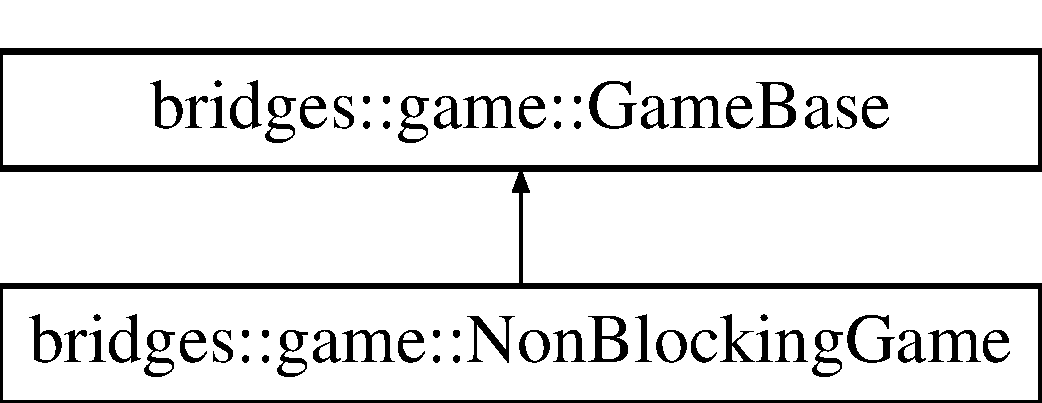
\includegraphics[height=2.000000cm]{classbridges_1_1game_1_1_non_blocking_game}
\end{center}
\end{figure}


\doxysubsection{Detailed Description}
This class provides the features necessary to implement simple non blocking games. 

The games that can be created out of \mbox{\hyperlink{classbridges_1_1game_1_1_non_blocking_game}{Non\+Blocking\+Game}} are based on a simple board grid of at most 1024 cells (e.\+g., 32x32, or any combinations less than 1024 cells). Each cell has a background color, and a colored symbol.

This class is used by having another class derive from it and implement the two functions\+: \mbox{\hyperlink{classbridges_1_1game_1_1_game_base_a9b6eb6fa7fceaac09d204b549164037f}{initialize()}} and Game\+Loop(). \mbox{\hyperlink{classbridges_1_1game_1_1_game_base_a9b6eb6fa7fceaac09d204b549164037f}{initialize()}} is called exactly once, on the first frame of the game. It is used to make first time initializations of the game state (such as setting the board in its initial position, for instance in chess). However, Game\+Loop() is called at every frame of the game. The game starts when the function \mbox{\hyperlink{classbridges_1_1game_1_1_non_blocking_game_ab48a0d690368bb8ff7b02aad0b6f336e}{start()}} is called on the object you created.

For this reason the simplest game that can run is created by\+:


\begin{DoxyCode}{0}
\DoxyCodeLine{\textcolor{preprocessor}{\#include <\mbox{\hyperlink{_non_blocking_game_8h}{NonBlockingGame.h}}>}}
\DoxyCodeLine{\textcolor{keyword}{using namespace }\mbox{\hyperlink{namespacebridges_1_1game}{bridges::game}};}
\DoxyCodeLine{\textcolor{keyword}{struct }my\_game : \textcolor{keyword}{public} \mbox{\hyperlink{classbridges_1_1game_1_1_non_blocking_game_a3226aa7e7ff129e916f4bd5aabcb2e72}{NonBlockingGame}} \{}
\DoxyCodeLine{  my\_game() : \mbox{\hyperlink{classbridges_1_1game_1_1_non_blocking_game_a3226aa7e7ff129e916f4bd5aabcb2e72}{NonBlockingGame}} (1, \textcolor{stringliteral}{"{}myuserid"{}},  \textcolor{stringliteral}{"{}myapikey"{}}) \{\}}
\DoxyCodeLine{  \textcolor{keyword}{virtual} \textcolor{keywordtype}{void} \mbox{\hyperlink{classbridges_1_1game_1_1_game_base_a9b6eb6fa7fceaac09d204b549164037f}{initialize}}()\textcolor{keyword}{ override }\{ \}}
\DoxyCodeLine{  \textcolor{keyword}{virtual} \textcolor{keywordtype}{void} GameLoop()\textcolor{keyword}{ override }\{ \}}
\DoxyCodeLine{\};}
\DoxyCodeLine{}
\DoxyCodeLine{\textcolor{keywordtype}{int} main () \{}
\DoxyCodeLine{  my\_game \mbox{\hyperlink{namespacebridges_1_1game_ab9a19c7ab6e2ebac2f95180e21733487ab2f5ff47436671b6e533d8dc3614845d}{g}};}
\DoxyCodeLine{  \mbox{\hyperlink{namespacebridges_1_1game_ab9a19c7ab6e2ebac2f95180e21733487ab2f5ff47436671b6e533d8dc3614845d}{g}}.start();}
\DoxyCodeLine{\}}

\end{DoxyCode}


This game does not do anything, but it is the minimal code that will run a game. Note that the constructor of my\+\_\+game passes 3 parameters to the constructor of \mbox{\hyperlink{classbridges_1_1game_1_1_non_blocking_game_a3226aa7e7ff129e916f4bd5aabcb2e72}{Non\+Blocking\+Game()}}. These three parameters are the classic parameters that the constructor of \mbox{\hyperlink{classbridges_1_1_bridges}{bridges\+::\+Bridges}} takes (e.\+g., assignment\+ID, username, apikey).

To change the board, two functions are used. \mbox{\hyperlink{classbridges_1_1game_1_1_game_base_ab667bbca1c81e5fb3aa8d81d70fe8cd2}{set\+BGColor()}} change the background color of a particular cell. It takes three parameters, the first two identify the cell of the board to change, and the last one is a color from a color palette provided by Named\+Color. \mbox{\hyperlink{classbridges_1_1game_1_1_game_base_a415fa8f70bef364dfa966f2a86048901}{draw\+Symbol()}} takes four parameters, the first two identify the cell of the board to change, the third is a symbol from a symbol palette provided by Named\+Symbol, the fourth is the color that symbol shold be drawn in and provided by Named\+Color.

For instance, a very simple \mbox{\hyperlink{classbridges_1_1game_1_1_game_base_a9b6eb6fa7fceaac09d204b549164037f}{initialize()}} could look like\+: 
\begin{DoxyCode}{0}
\DoxyCodeLine{\textcolor{keyword}{virtual} \textcolor{keywordtype}{void} \mbox{\hyperlink{classbridges_1_1game_1_1_game_base_a9b6eb6fa7fceaac09d204b549164037f}{initialize}}()\textcolor{keyword}{ override }\{}
\DoxyCodeLine{  \mbox{\hyperlink{classbridges_1_1game_1_1_game_base_ab667bbca1c81e5fb3aa8d81d70fe8cd2}{setBGColor}}(0, 0, \mbox{\hyperlink{namespacebridges_1_1game_afaa832a4322b25b6a4ebfba832f10f26}{NamedColor}}.lightsalmon);}
\DoxyCodeLine{  \mbox{\hyperlink{classbridges_1_1game_1_1_game_base_a415fa8f70bef364dfa966f2a86048901}{drawSymbol}}(0, 0, \mbox{\hyperlink{namespacebridges_1_1game_ab9a19c7ab6e2ebac2f95180e21733487}{NamedSymbol}}.sword, \mbox{\hyperlink{namespacebridges_1_1game_afaa832a4322b25b6a4ebfba832f10f26}{NamedColor}}.blue);}
\DoxyCodeLine{\}}

\end{DoxyCode}


Note that the size of the board is set by default at 10x10 and that drawing on a cell that does not exist will lead to an error. One can specify a gameboard of a different size by passing additional parameters to the \mbox{\hyperlink{classbridges_1_1game_1_1_non_blocking_game}{Non\+Blocking\+Game}} constructor. However, the game can not be more than 1024 cells in total, so a 15x15 board is possible, a 32x32 board is the largest square board possible, and a rectangular 64x16 rectangular board is also possible. But a 100x20 board would be 2000 cells and is not possible. For instance a board of 16 rows and 64 columns can be created defining the my\+\_\+game constructor as\+:


\begin{DoxyCode}{0}
\DoxyCodeLine{my\_game() : \mbox{\hyperlink{classbridges_1_1game_1_1_non_blocking_game_a3226aa7e7ff129e916f4bd5aabcb2e72}{NonBlockingGame}} (1, \textcolor{stringliteral}{"{}myuserid"{}},  \textcolor{stringliteral}{"{}myapikey"{}}, 16, 64) \{\}}

\end{DoxyCode}


The bridges game engine will call the Game\+Loop() function at each frame of the game. You can write this function to modify the state of the game board using \mbox{\hyperlink{classbridges_1_1game_1_1_game_base_ab667bbca1c81e5fb3aa8d81d70fe8cd2}{set\+BGColor()}} and \mbox{\hyperlink{classbridges_1_1game_1_1_game_base_a415fa8f70bef364dfa966f2a86048901}{draw\+Symbol()}}. For instance, the following Game\+Loop() will color the board randomly one cell at a time.


\begin{DoxyCode}{0}
\DoxyCodeLine{\textcolor{keyword}{virtual} \textcolor{keywordtype}{void} \mbox{\hyperlink{classbridges_1_1game_1_1_game_base_a16fb787bc65be1a582cddcfba3a0c5bb}{gameLoop}}()\textcolor{keyword}{ override }\{}
\DoxyCodeLine{  \mbox{\hyperlink{classbridges_1_1game_1_1_game_base_ab667bbca1c81e5fb3aa8d81d70fe8cd2}{setBGColor}}(rand()\%10, rand()\%10, \mbox{\hyperlink{namespacebridges_1_1game_afaa832a4322b25b6a4ebfba832f10f26}{NamedColor}}.lightsalmon);}
\DoxyCodeLine{\}}

\end{DoxyCode}


The game\+Loop can also probe the state of some keys of the keyboard using functions \mbox{\hyperlink{classbridges_1_1game_1_1_non_blocking_game_a0a93cf74e7eac55c33f76cd55d525084}{key\+Up()}}, \mbox{\hyperlink{classbridges_1_1game_1_1_non_blocking_game_a9b7ba679dd177b28f84ea24b9924a51c}{key\+Left()}}, \mbox{\hyperlink{classbridges_1_1game_1_1_non_blocking_game_a52dd79aaaee9da77fa392fb8ec37fa94}{key\+Down()}}, \mbox{\hyperlink{classbridges_1_1game_1_1_non_blocking_game_afbea1fa2acec16e952be66ce76d496a9}{key\+Right()}}, \mbox{\hyperlink{classbridges_1_1game_1_1_non_blocking_game_a7bd5c2ab845e24525649dda7f8dfd460}{key\+W()}}, \mbox{\hyperlink{classbridges_1_1game_1_1_non_blocking_game_af88089437e34df580b247cb27047fd14}{key\+A()}}, \mbox{\hyperlink{classbridges_1_1game_1_1_non_blocking_game_a75ece5d4fa35893ecacc82c5064c05e0}{key\+S()}}, \mbox{\hyperlink{classbridges_1_1game_1_1_non_blocking_game_a932979445cc8acea618092b83b4a9756}{key\+D()}}, \mbox{\hyperlink{classbridges_1_1game_1_1_non_blocking_game_a54beca154b58b0e0fb26c75983ba5072}{key\+Space()}}, and \mbox{\hyperlink{classbridges_1_1game_1_1_non_blocking_game_af0dafefbad315fbfb01851a4a0dfa93e}{key\+Q()}}. These functions return a boolean that indicate whether the key is pressed at that frame or not. For instance, the following code will only color the board randomly when the up arrow is pressed.


\begin{DoxyCode}{0}
\DoxyCodeLine{\textcolor{keyword}{virtual} \textcolor{keywordtype}{void} \mbox{\hyperlink{classbridges_1_1game_1_1_game_base_a16fb787bc65be1a582cddcfba3a0c5bb}{gameLoop}}()\textcolor{keyword}{ override }\{}
\DoxyCodeLine{  \textcolor{keywordflow}{if} (\mbox{\hyperlink{classbridges_1_1game_1_1_non_blocking_game_a0a93cf74e7eac55c33f76cd55d525084}{keyUp}}())}
\DoxyCodeLine{    \mbox{\hyperlink{classbridges_1_1game_1_1_game_base_ab667bbca1c81e5fb3aa8d81d70fe8cd2}{setBGColor}}(rand()\%10, rand()\%10, \mbox{\hyperlink{namespacebridges_1_1game_afaa832a4322b25b6a4ebfba832f10f26}{NamedColor}}.lightsalmon);}
\DoxyCodeLine{\}}

\end{DoxyCode}


\begin{DoxySeeAlso}{See also}
There is a tutorial at\+: \href{https://bridgesuncc.github.io/tutorials/NonBlockingGame.html}{\texttt{ https\+://bridgesuncc.\+github.\+io/tutorials/\+Non\+Blocking\+Game.\+html}}
\end{DoxySeeAlso}
\begin{DoxyAuthor}{Author}
Erik Saule 
\end{DoxyAuthor}
\begin{DoxyDate}{Date}
7/21/19, 12/28/20 
\end{DoxyDate}
\doxysubsection*{Public Member Functions}
\begin{DoxyCompactItemize}
\item 
\mbox{\hyperlink{classbridges_1_1game_1_1_non_blocking_game_a3226aa7e7ff129e916f4bd5aabcb2e72}{Non\+Blocking\+Game}} (int assignment\+ID, std\+::string username, std\+::string apikey, int nb\+Row=10, int nb\+Col=10)
\item 
void \mbox{\hyperlink{classbridges_1_1game_1_1_non_blocking_game_ab48a0d690368bb8ff7b02aad0b6f336e}{start}} ()
\begin{DoxyCompactList}\small\item\em Call this function from main to start the game. Runs exactly once. \end{DoxyCompactList}\end{DoxyCompactItemize}
\doxysubsection*{Protected Member Functions}
\begin{DoxyCompactItemize}
\item 
double \mbox{\hyperlink{classbridges_1_1game_1_1_non_blocking_game_ab3bee2db9d0d2c4e74ae7943516fb53a}{get\+Frame\+Rate}} () const
\begin{DoxyCompactList}\small\item\em What frame rate is the game running at? \end{DoxyCompactList}\item 
bool \mbox{\hyperlink{classbridges_1_1game_1_1_non_blocking_game_a9b7ba679dd177b28f84ea24b9924a51c}{key\+Left}} ()
\begin{DoxyCompactList}\small\item\em Is Left currently pressed? \end{DoxyCompactList}\item 
bool \mbox{\hyperlink{classbridges_1_1game_1_1_non_blocking_game_afbea1fa2acec16e952be66ce76d496a9}{key\+Right}} ()
\begin{DoxyCompactList}\small\item\em Is Right currently pressed? \end{DoxyCompactList}\item 
bool \mbox{\hyperlink{classbridges_1_1game_1_1_non_blocking_game_a0a93cf74e7eac55c33f76cd55d525084}{key\+Up}} ()
\begin{DoxyCompactList}\small\item\em Is Up currently pressed? \end{DoxyCompactList}\item 
bool \mbox{\hyperlink{classbridges_1_1game_1_1_non_blocking_game_a52dd79aaaee9da77fa392fb8ec37fa94}{key\+Down}} ()
\begin{DoxyCompactList}\small\item\em Is Down currently pressed? \end{DoxyCompactList}\item 
bool \mbox{\hyperlink{classbridges_1_1game_1_1_non_blocking_game_a7bd5c2ab845e24525649dda7f8dfd460}{keyW}} ()
\begin{DoxyCompactList}\small\item\em Is W currently pressed? \end{DoxyCompactList}\item 
bool \mbox{\hyperlink{classbridges_1_1game_1_1_non_blocking_game_af88089437e34df580b247cb27047fd14}{keyA}} ()
\begin{DoxyCompactList}\small\item\em Is A currently pressed? \end{DoxyCompactList}\item 
bool \mbox{\hyperlink{classbridges_1_1game_1_1_non_blocking_game_a75ece5d4fa35893ecacc82c5064c05e0}{keyS}} ()
\begin{DoxyCompactList}\small\item\em Is S currently pressed? \end{DoxyCompactList}\item 
bool \mbox{\hyperlink{classbridges_1_1game_1_1_non_blocking_game_a932979445cc8acea618092b83b4a9756}{keyD}} ()
\begin{DoxyCompactList}\small\item\em Is D currently pressed? \end{DoxyCompactList}\item 
bool \mbox{\hyperlink{classbridges_1_1game_1_1_non_blocking_game_af0dafefbad315fbfb01851a4a0dfa93e}{keyQ}} ()
\begin{DoxyCompactList}\small\item\em Is Q currently pressed? \end{DoxyCompactList}\item 
bool \mbox{\hyperlink{classbridges_1_1game_1_1_non_blocking_game_a54beca154b58b0e0fb26c75983ba5072}{key\+Space}} ()
\begin{DoxyCompactList}\small\item\em Is Space currently pressed? \end{DoxyCompactList}\end{DoxyCompactItemize}
\doxysubsection*{Additional Inherited Members}


\doxysubsection{Constructor \& Destructor Documentation}
\mbox{\Hypertarget{classbridges_1_1game_1_1_non_blocking_game_a3226aa7e7ff129e916f4bd5aabcb2e72}\label{classbridges_1_1game_1_1_non_blocking_game_a3226aa7e7ff129e916f4bd5aabcb2e72}} 
\index{bridges::game::NonBlockingGame@{bridges::game::NonBlockingGame}!NonBlockingGame@{NonBlockingGame}}
\index{NonBlockingGame@{NonBlockingGame}!bridges::game::NonBlockingGame@{bridges::game::NonBlockingGame}}
\doxysubsubsection{\texorpdfstring{NonBlockingGame()}{NonBlockingGame()}}
{\footnotesize\ttfamily bridges\+::game\+::\+Non\+Blocking\+Game\+::\+Non\+Blocking\+Game (\begin{DoxyParamCaption}\item[{int}]{assignment\+ID,  }\item[{std\+::string}]{username,  }\item[{std\+::string}]{apikey,  }\item[{int}]{nb\+Row = {\ttfamily 10},  }\item[{int}]{nb\+Col = {\ttfamily 10} }\end{DoxyParamCaption})\hspace{0.3cm}{\ttfamily [inline]}}

constructor 
\begin{DoxyParams}{Parameters}
{\em assignment\+ID} & \mbox{\hyperlink{classbridges_1_1_bridges}{Bridges}} assignment id \\
\hline
{\em username} & \mbox{\hyperlink{classbridges_1_1_bridges}{Bridges}} user name \\
\hline
{\em apikey} & \mbox{\hyperlink{classbridges_1_1_bridges}{Bridges}} API authentication key \\
\hline
{\em nb\+Row} & \mbox{\hyperlink{classbridges_1_1game_1_1_game_grid}{Game\+Grid}} height \\
\hline
{\em nb\+Col} & \mbox{\hyperlink{classbridges_1_1game_1_1_game_grid}{Game\+Grid}} width \\
\hline
\end{DoxyParams}


\doxysubsection{Member Function Documentation}
\mbox{\Hypertarget{classbridges_1_1game_1_1_non_blocking_game_ab3bee2db9d0d2c4e74ae7943516fb53a}\label{classbridges_1_1game_1_1_non_blocking_game_ab3bee2db9d0d2c4e74ae7943516fb53a}} 
\index{bridges::game::NonBlockingGame@{bridges::game::NonBlockingGame}!getFrameRate@{getFrameRate}}
\index{getFrameRate@{getFrameRate}!bridges::game::NonBlockingGame@{bridges::game::NonBlockingGame}}
\doxysubsubsection{\texorpdfstring{getFrameRate()}{getFrameRate()}}
{\footnotesize\ttfamily double bridges\+::game\+::\+Non\+Blocking\+Game\+::get\+Frame\+Rate (\begin{DoxyParamCaption}{ }\end{DoxyParamCaption}) const\hspace{0.3cm}{\ttfamily [inline]}, {\ttfamily [protected]}}



What frame rate is the game running at? 

\begin{DoxyReturn}{Returns}
the target framerate. The game could be somewhat slower depending on how computationally expensive the gameloop is and on the speed of the network. 
\end{DoxyReturn}
\mbox{\Hypertarget{classbridges_1_1game_1_1_non_blocking_game_af88089437e34df580b247cb27047fd14}\label{classbridges_1_1game_1_1_non_blocking_game_af88089437e34df580b247cb27047fd14}} 
\index{bridges::game::NonBlockingGame@{bridges::game::NonBlockingGame}!keyA@{keyA}}
\index{keyA@{keyA}!bridges::game::NonBlockingGame@{bridges::game::NonBlockingGame}}
\doxysubsubsection{\texorpdfstring{keyA()}{keyA()}}
{\footnotesize\ttfamily bool bridges\+::game\+::\+Non\+Blocking\+Game\+::keyA (\begin{DoxyParamCaption}{ }\end{DoxyParamCaption})\hspace{0.3cm}{\ttfamily [inline]}, {\ttfamily [protected]}}



Is A currently pressed? 

\begin{DoxyReturn}{Returns}
true if A is currently pressed 
\end{DoxyReturn}
\mbox{\Hypertarget{classbridges_1_1game_1_1_non_blocking_game_a932979445cc8acea618092b83b4a9756}\label{classbridges_1_1game_1_1_non_blocking_game_a932979445cc8acea618092b83b4a9756}} 
\index{bridges::game::NonBlockingGame@{bridges::game::NonBlockingGame}!keyD@{keyD}}
\index{keyD@{keyD}!bridges::game::NonBlockingGame@{bridges::game::NonBlockingGame}}
\doxysubsubsection{\texorpdfstring{keyD()}{keyD()}}
{\footnotesize\ttfamily bool bridges\+::game\+::\+Non\+Blocking\+Game\+::keyD (\begin{DoxyParamCaption}{ }\end{DoxyParamCaption})\hspace{0.3cm}{\ttfamily [inline]}, {\ttfamily [protected]}}



Is D currently pressed? 

\begin{DoxyReturn}{Returns}
true if D is currently pressed 
\end{DoxyReturn}
\mbox{\Hypertarget{classbridges_1_1game_1_1_non_blocking_game_a52dd79aaaee9da77fa392fb8ec37fa94}\label{classbridges_1_1game_1_1_non_blocking_game_a52dd79aaaee9da77fa392fb8ec37fa94}} 
\index{bridges::game::NonBlockingGame@{bridges::game::NonBlockingGame}!keyDown@{keyDown}}
\index{keyDown@{keyDown}!bridges::game::NonBlockingGame@{bridges::game::NonBlockingGame}}
\doxysubsubsection{\texorpdfstring{keyDown()}{keyDown()}}
{\footnotesize\ttfamily bool bridges\+::game\+::\+Non\+Blocking\+Game\+::key\+Down (\begin{DoxyParamCaption}{ }\end{DoxyParamCaption})\hspace{0.3cm}{\ttfamily [inline]}, {\ttfamily [protected]}}



Is Down currently pressed? 

\begin{DoxyReturn}{Returns}
true if Down is currently pressed 
\end{DoxyReturn}
\mbox{\Hypertarget{classbridges_1_1game_1_1_non_blocking_game_a9b7ba679dd177b28f84ea24b9924a51c}\label{classbridges_1_1game_1_1_non_blocking_game_a9b7ba679dd177b28f84ea24b9924a51c}} 
\index{bridges::game::NonBlockingGame@{bridges::game::NonBlockingGame}!keyLeft@{keyLeft}}
\index{keyLeft@{keyLeft}!bridges::game::NonBlockingGame@{bridges::game::NonBlockingGame}}
\doxysubsubsection{\texorpdfstring{keyLeft()}{keyLeft()}}
{\footnotesize\ttfamily bool bridges\+::game\+::\+Non\+Blocking\+Game\+::key\+Left (\begin{DoxyParamCaption}{ }\end{DoxyParamCaption})\hspace{0.3cm}{\ttfamily [inline]}, {\ttfamily [protected]}}



Is Left currently pressed? 

\begin{DoxyReturn}{Returns}
true if Left is currently pressed 
\end{DoxyReturn}
\mbox{\Hypertarget{classbridges_1_1game_1_1_non_blocking_game_af0dafefbad315fbfb01851a4a0dfa93e}\label{classbridges_1_1game_1_1_non_blocking_game_af0dafefbad315fbfb01851a4a0dfa93e}} 
\index{bridges::game::NonBlockingGame@{bridges::game::NonBlockingGame}!keyQ@{keyQ}}
\index{keyQ@{keyQ}!bridges::game::NonBlockingGame@{bridges::game::NonBlockingGame}}
\doxysubsubsection{\texorpdfstring{keyQ()}{keyQ()}}
{\footnotesize\ttfamily bool bridges\+::game\+::\+Non\+Blocking\+Game\+::keyQ (\begin{DoxyParamCaption}{ }\end{DoxyParamCaption})\hspace{0.3cm}{\ttfamily [inline]}, {\ttfamily [protected]}}



Is Q currently pressed? 

\begin{DoxyReturn}{Returns}
true if S is currently pressed 
\end{DoxyReturn}
\mbox{\Hypertarget{classbridges_1_1game_1_1_non_blocking_game_afbea1fa2acec16e952be66ce76d496a9}\label{classbridges_1_1game_1_1_non_blocking_game_afbea1fa2acec16e952be66ce76d496a9}} 
\index{bridges::game::NonBlockingGame@{bridges::game::NonBlockingGame}!keyRight@{keyRight}}
\index{keyRight@{keyRight}!bridges::game::NonBlockingGame@{bridges::game::NonBlockingGame}}
\doxysubsubsection{\texorpdfstring{keyRight()}{keyRight()}}
{\footnotesize\ttfamily bool bridges\+::game\+::\+Non\+Blocking\+Game\+::key\+Right (\begin{DoxyParamCaption}{ }\end{DoxyParamCaption})\hspace{0.3cm}{\ttfamily [inline]}, {\ttfamily [protected]}}



Is Right currently pressed? 

\begin{DoxyReturn}{Returns}
true if Right is currently pressed 
\end{DoxyReturn}
\mbox{\Hypertarget{classbridges_1_1game_1_1_non_blocking_game_a75ece5d4fa35893ecacc82c5064c05e0}\label{classbridges_1_1game_1_1_non_blocking_game_a75ece5d4fa35893ecacc82c5064c05e0}} 
\index{bridges::game::NonBlockingGame@{bridges::game::NonBlockingGame}!keyS@{keyS}}
\index{keyS@{keyS}!bridges::game::NonBlockingGame@{bridges::game::NonBlockingGame}}
\doxysubsubsection{\texorpdfstring{keyS()}{keyS()}}
{\footnotesize\ttfamily bool bridges\+::game\+::\+Non\+Blocking\+Game\+::keyS (\begin{DoxyParamCaption}{ }\end{DoxyParamCaption})\hspace{0.3cm}{\ttfamily [inline]}, {\ttfamily [protected]}}



Is S currently pressed? 

\begin{DoxyReturn}{Returns}
true if S is currently pressed 
\end{DoxyReturn}
\mbox{\Hypertarget{classbridges_1_1game_1_1_non_blocking_game_a54beca154b58b0e0fb26c75983ba5072}\label{classbridges_1_1game_1_1_non_blocking_game_a54beca154b58b0e0fb26c75983ba5072}} 
\index{bridges::game::NonBlockingGame@{bridges::game::NonBlockingGame}!keySpace@{keySpace}}
\index{keySpace@{keySpace}!bridges::game::NonBlockingGame@{bridges::game::NonBlockingGame}}
\doxysubsubsection{\texorpdfstring{keySpace()}{keySpace()}}
{\footnotesize\ttfamily bool bridges\+::game\+::\+Non\+Blocking\+Game\+::key\+Space (\begin{DoxyParamCaption}{ }\end{DoxyParamCaption})\hspace{0.3cm}{\ttfamily [inline]}, {\ttfamily [protected]}}



Is Space currently pressed? 

\begin{DoxyReturn}{Returns}
true if Space is currently pressed 
\end{DoxyReturn}
\mbox{\Hypertarget{classbridges_1_1game_1_1_non_blocking_game_a0a93cf74e7eac55c33f76cd55d525084}\label{classbridges_1_1game_1_1_non_blocking_game_a0a93cf74e7eac55c33f76cd55d525084}} 
\index{bridges::game::NonBlockingGame@{bridges::game::NonBlockingGame}!keyUp@{keyUp}}
\index{keyUp@{keyUp}!bridges::game::NonBlockingGame@{bridges::game::NonBlockingGame}}
\doxysubsubsection{\texorpdfstring{keyUp()}{keyUp()}}
{\footnotesize\ttfamily bool bridges\+::game\+::\+Non\+Blocking\+Game\+::key\+Up (\begin{DoxyParamCaption}{ }\end{DoxyParamCaption})\hspace{0.3cm}{\ttfamily [inline]}, {\ttfamily [protected]}}



Is Up currently pressed? 

\begin{DoxyReturn}{Returns}
true if Up is currently pressed 
\end{DoxyReturn}
\mbox{\Hypertarget{classbridges_1_1game_1_1_non_blocking_game_a7bd5c2ab845e24525649dda7f8dfd460}\label{classbridges_1_1game_1_1_non_blocking_game_a7bd5c2ab845e24525649dda7f8dfd460}} 
\index{bridges::game::NonBlockingGame@{bridges::game::NonBlockingGame}!keyW@{keyW}}
\index{keyW@{keyW}!bridges::game::NonBlockingGame@{bridges::game::NonBlockingGame}}
\doxysubsubsection{\texorpdfstring{keyW()}{keyW()}}
{\footnotesize\ttfamily bool bridges\+::game\+::\+Non\+Blocking\+Game\+::keyW (\begin{DoxyParamCaption}{ }\end{DoxyParamCaption})\hspace{0.3cm}{\ttfamily [inline]}, {\ttfamily [protected]}}



Is W currently pressed? 

\begin{DoxyReturn}{Returns}
true if W is currently pressed 
\end{DoxyReturn}
\mbox{\Hypertarget{classbridges_1_1game_1_1_non_blocking_game_ab48a0d690368bb8ff7b02aad0b6f336e}\label{classbridges_1_1game_1_1_non_blocking_game_ab48a0d690368bb8ff7b02aad0b6f336e}} 
\index{bridges::game::NonBlockingGame@{bridges::game::NonBlockingGame}!start@{start}}
\index{start@{start}!bridges::game::NonBlockingGame@{bridges::game::NonBlockingGame}}
\doxysubsubsection{\texorpdfstring{start()}{start()}}
{\footnotesize\ttfamily void bridges\+::game\+::\+Non\+Blocking\+Game\+::start (\begin{DoxyParamCaption}{ }\end{DoxyParamCaption})\hspace{0.3cm}{\ttfamily [inline]}}



Call this function from main to start the game. Runs exactly once. 



The documentation for this class was generated from the following file\+:\begin{DoxyCompactItemize}
\item 
/home/erik/work/bridges/bridges-\/cxx/src/\mbox{\hyperlink{_non_blocking_game_8h}{Non\+Blocking\+Game.\+h}}\end{DoxyCompactItemize}

\hypertarget{classsio_1_1null__message}{}\doxysection{sio\+::null\+\_\+message Class Reference}
\label{classsio_1_1null__message}\index{sio::null\_message@{sio::null\_message}}


{\ttfamily \#include $<$sio\+\_\+message.\+h$>$}

Inheritance diagram for sio\+::null\+\_\+message\+:\begin{figure}[H]
\begin{center}
\leavevmode
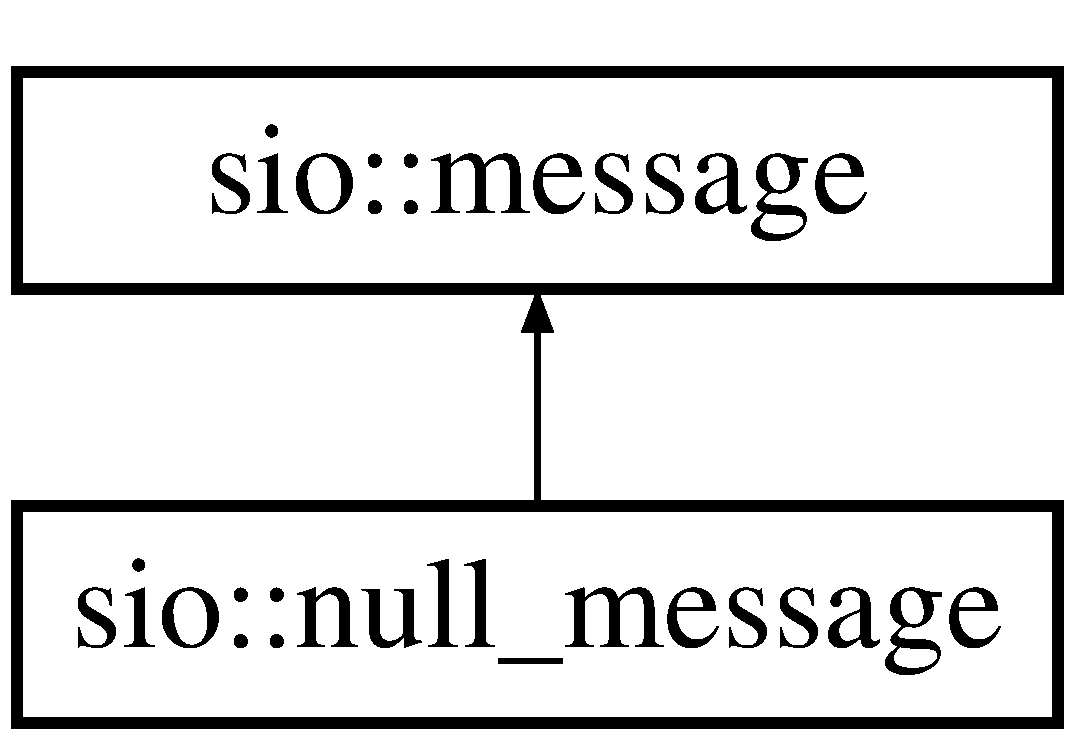
\includegraphics[height=2.000000cm]{classsio_1_1null__message}
\end{center}
\end{figure}
\doxysubsection*{Static Public Member Functions}
\begin{DoxyCompactItemize}
\item 
static \mbox{\hyperlink{classsio_1_1message_a6340b6fef57e4516eb17928b1885a615}{message\+::ptr}} \mbox{\hyperlink{classsio_1_1null__message_a829d67c9ff528a8eef8597c58e868802}{create}} ()
\end{DoxyCompactItemize}
\doxysubsection*{Protected Member Functions}
\begin{DoxyCompactItemize}
\item 
\mbox{\hyperlink{classsio_1_1null__message_a1518dd808081df4b79a753ead398f902}{null\+\_\+message}} ()
\end{DoxyCompactItemize}
\doxysubsection*{Additional Inherited Members}


\doxysubsection{Constructor \& Destructor Documentation}
\mbox{\Hypertarget{classsio_1_1null__message_a1518dd808081df4b79a753ead398f902}\label{classsio_1_1null__message_a1518dd808081df4b79a753ead398f902}} 
\index{sio::null\_message@{sio::null\_message}!null\_message@{null\_message}}
\index{null\_message@{null\_message}!sio::null\_message@{sio::null\_message}}
\doxysubsubsection{\texorpdfstring{null\_message()}{null\_message()}}
{\footnotesize\ttfamily sio\+::null\+\_\+message\+::null\+\_\+message (\begin{DoxyParamCaption}{ }\end{DoxyParamCaption})\hspace{0.3cm}{\ttfamily [inline]}, {\ttfamily [protected]}}



\doxysubsection{Member Function Documentation}
\mbox{\Hypertarget{classsio_1_1null__message_a829d67c9ff528a8eef8597c58e868802}\label{classsio_1_1null__message_a829d67c9ff528a8eef8597c58e868802}} 
\index{sio::null\_message@{sio::null\_message}!create@{create}}
\index{create@{create}!sio::null\_message@{sio::null\_message}}
\doxysubsubsection{\texorpdfstring{create()}{create()}}
{\footnotesize\ttfamily static \mbox{\hyperlink{classsio_1_1message_a6340b6fef57e4516eb17928b1885a615}{message\+::ptr}} sio\+::null\+\_\+message\+::create (\begin{DoxyParamCaption}{ }\end{DoxyParamCaption})\hspace{0.3cm}{\ttfamily [inline]}, {\ttfamily [static]}}



The documentation for this class was generated from the following file\+:\begin{DoxyCompactItemize}
\item 
/home/erik/work/bridges/bridges-\/cxx/src/\mbox{\hyperlink{sio__message_8h}{sio\+\_\+message.\+h}}\end{DoxyCompactItemize}

\hypertarget{classsio_1_1object__message}{}\doxysection{sio\+::object\+\_\+message Class Reference}
\label{classsio_1_1object__message}\index{sio::object\_message@{sio::object\_message}}


{\ttfamily \#include $<$sio\+\_\+message.\+h$>$}

Inheritance diagram for sio\+::object\+\_\+message\+:\begin{figure}[H]
\begin{center}
\leavevmode
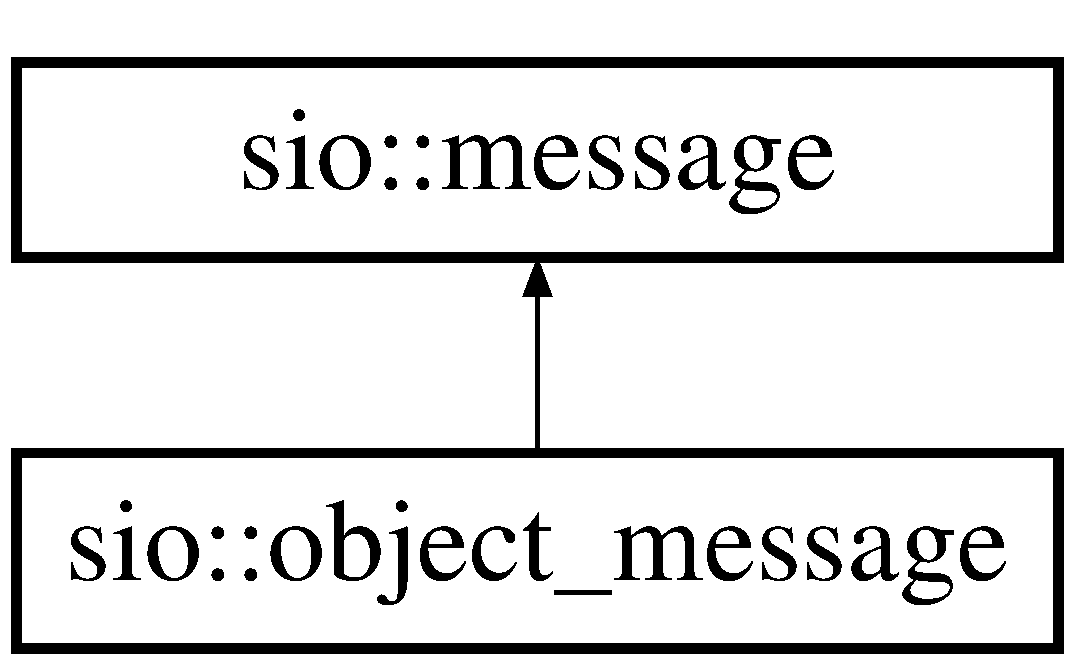
\includegraphics[height=2.000000cm]{classsio_1_1object__message}
\end{center}
\end{figure}
\doxysubsection*{Public Member Functions}
\begin{DoxyCompactItemize}
\item 
void \mbox{\hyperlink{classsio_1_1object__message_a1d12ae0a5f6820f54d47e8c84f2f2316}{insert}} (const std\+::string \&key, \mbox{\hyperlink{classsio_1_1message_a6340b6fef57e4516eb17928b1885a615}{message\+::ptr}} const \&\mbox{\hyperlink{classsio_1_1message}{message}})
\item 
void \mbox{\hyperlink{classsio_1_1object__message_a1d00380eb3c8bef206aeeaffc2a9d1e0}{insert}} (const std\+::string \&key, const std\+::string \&text)
\item 
void \mbox{\hyperlink{classsio_1_1object__message_a3932caf1b59398c1a7bf07720614f0b0}{insert}} (const std\+::string \&key, std\+::string \&\&text)
\item 
void \mbox{\hyperlink{classsio_1_1object__message_a8070cf3c80b9f02cb66e0e767666b30f}{insert}} (const std\+::string \&key, std\+::shared\+\_\+ptr$<$ std\+::string $>$ const \&binary)
\item 
void \mbox{\hyperlink{classsio_1_1object__message_aa0c14900ec41c99e1507299a3ee8c7f1}{insert}} (const std\+::string \&key, std\+::shared\+\_\+ptr$<$ const std\+::string $>$ const \&binary)
\item 
bool \mbox{\hyperlink{classsio_1_1object__message_a2afede757162e3c5e70919a47da9d4f0}{has}} (const std\+::string \&key)
\item 
const \mbox{\hyperlink{classsio_1_1message_a6340b6fef57e4516eb17928b1885a615}{message\+::ptr}} \& \mbox{\hyperlink{classsio_1_1object__message_ac2ca0303720d11347e7de69592db9999}{at}} (const std\+::string \&key) const
\item 
const \mbox{\hyperlink{classsio_1_1message_a6340b6fef57e4516eb17928b1885a615}{message\+::ptr}} \& \mbox{\hyperlink{classsio_1_1object__message_a52c7af95802da3f3e3a56a8509e329ee}{operator\mbox{[}$\,$\mbox{]}}} (const std\+::string \&key) const
\item 
bool \mbox{\hyperlink{classsio_1_1object__message_a7b34b62fbd7d8f681509e28b3695d235}{has}} (const std\+::string \&key) const
\item 
std\+::map$<$ std\+::string, \mbox{\hyperlink{classsio_1_1message_a6340b6fef57e4516eb17928b1885a615}{message\+::ptr}} $>$ \& \mbox{\hyperlink{classsio_1_1object__message_ac024fab0eb24248150ab318a4b937b4e}{get\+\_\+map}} ()
\item 
const std\+::map$<$ std\+::string, \mbox{\hyperlink{classsio_1_1message_a6340b6fef57e4516eb17928b1885a615}{message\+::ptr}} $>$ \& \mbox{\hyperlink{classsio_1_1object__message_a35d7f1d654b2a3b753ac01444635203e}{get\+\_\+map}} () const
\end{DoxyCompactItemize}
\doxysubsection*{Static Public Member Functions}
\begin{DoxyCompactItemize}
\item 
static \mbox{\hyperlink{classsio_1_1message_a6340b6fef57e4516eb17928b1885a615}{message\+::ptr}} \mbox{\hyperlink{classsio_1_1object__message_ab100c2e474a1c17bfd93009076cdb6a8}{create}} ()
\end{DoxyCompactItemize}
\doxysubsection*{Additional Inherited Members}


\doxysubsection{Member Function Documentation}
\mbox{\Hypertarget{classsio_1_1object__message_ac2ca0303720d11347e7de69592db9999}\label{classsio_1_1object__message_ac2ca0303720d11347e7de69592db9999}} 
\index{sio::object\_message@{sio::object\_message}!at@{at}}
\index{at@{at}!sio::object\_message@{sio::object\_message}}
\doxysubsubsection{\texorpdfstring{at()}{at()}}
{\footnotesize\ttfamily const \mbox{\hyperlink{classsio_1_1message_a6340b6fef57e4516eb17928b1885a615}{message\+::ptr}}\& sio\+::object\+\_\+message\+::at (\begin{DoxyParamCaption}\item[{const std\+::string \&}]{key }\end{DoxyParamCaption}) const\hspace{0.3cm}{\ttfamily [inline]}}

\mbox{\Hypertarget{classsio_1_1object__message_ab100c2e474a1c17bfd93009076cdb6a8}\label{classsio_1_1object__message_ab100c2e474a1c17bfd93009076cdb6a8}} 
\index{sio::object\_message@{sio::object\_message}!create@{create}}
\index{create@{create}!sio::object\_message@{sio::object\_message}}
\doxysubsubsection{\texorpdfstring{create()}{create()}}
{\footnotesize\ttfamily static \mbox{\hyperlink{classsio_1_1message_a6340b6fef57e4516eb17928b1885a615}{message\+::ptr}} sio\+::object\+\_\+message\+::create (\begin{DoxyParamCaption}{ }\end{DoxyParamCaption})\hspace{0.3cm}{\ttfamily [inline]}, {\ttfamily [static]}}

\mbox{\Hypertarget{classsio_1_1object__message_ac024fab0eb24248150ab318a4b937b4e}\label{classsio_1_1object__message_ac024fab0eb24248150ab318a4b937b4e}} 
\index{sio::object\_message@{sio::object\_message}!get\_map@{get\_map}}
\index{get\_map@{get\_map}!sio::object\_message@{sio::object\_message}}
\doxysubsubsection{\texorpdfstring{get\_map()}{get\_map()}\hspace{0.1cm}{\footnotesize\ttfamily [1/2]}}
{\footnotesize\ttfamily std\+::map$<$std\+::string, \mbox{\hyperlink{classsio_1_1message_a6340b6fef57e4516eb17928b1885a615}{message\+::ptr}}$>$\& sio\+::object\+\_\+message\+::get\+\_\+map (\begin{DoxyParamCaption}{ }\end{DoxyParamCaption})\hspace{0.3cm}{\ttfamily [inline]}, {\ttfamily [virtual]}}



Reimplemented from \mbox{\hyperlink{classsio_1_1message_a6ca4aee4616aa9dfde4de317d5efd125}{sio\+::message}}.

\mbox{\Hypertarget{classsio_1_1object__message_a35d7f1d654b2a3b753ac01444635203e}\label{classsio_1_1object__message_a35d7f1d654b2a3b753ac01444635203e}} 
\index{sio::object\_message@{sio::object\_message}!get\_map@{get\_map}}
\index{get\_map@{get\_map}!sio::object\_message@{sio::object\_message}}
\doxysubsubsection{\texorpdfstring{get\_map()}{get\_map()}\hspace{0.1cm}{\footnotesize\ttfamily [2/2]}}
{\footnotesize\ttfamily const std\+::map$<$std\+::string, \mbox{\hyperlink{classsio_1_1message_a6340b6fef57e4516eb17928b1885a615}{message\+::ptr}}$>$\& sio\+::object\+\_\+message\+::get\+\_\+map (\begin{DoxyParamCaption}{ }\end{DoxyParamCaption}) const\hspace{0.3cm}{\ttfamily [inline]}, {\ttfamily [virtual]}}



Reimplemented from \mbox{\hyperlink{classsio_1_1message_a954a981a468fcea36ff19cce6ae7fd5e}{sio\+::message}}.

\mbox{\Hypertarget{classsio_1_1object__message_a2afede757162e3c5e70919a47da9d4f0}\label{classsio_1_1object__message_a2afede757162e3c5e70919a47da9d4f0}} 
\index{sio::object\_message@{sio::object\_message}!has@{has}}
\index{has@{has}!sio::object\_message@{sio::object\_message}}
\doxysubsubsection{\texorpdfstring{has()}{has()}\hspace{0.1cm}{\footnotesize\ttfamily [1/2]}}
{\footnotesize\ttfamily bool sio\+::object\+\_\+message\+::has (\begin{DoxyParamCaption}\item[{const std\+::string \&}]{key }\end{DoxyParamCaption})\hspace{0.3cm}{\ttfamily [inline]}}

\mbox{\Hypertarget{classsio_1_1object__message_a7b34b62fbd7d8f681509e28b3695d235}\label{classsio_1_1object__message_a7b34b62fbd7d8f681509e28b3695d235}} 
\index{sio::object\_message@{sio::object\_message}!has@{has}}
\index{has@{has}!sio::object\_message@{sio::object\_message}}
\doxysubsubsection{\texorpdfstring{has()}{has()}\hspace{0.1cm}{\footnotesize\ttfamily [2/2]}}
{\footnotesize\ttfamily bool sio\+::object\+\_\+message\+::has (\begin{DoxyParamCaption}\item[{const std\+::string \&}]{key }\end{DoxyParamCaption}) const\hspace{0.3cm}{\ttfamily [inline]}}

\mbox{\Hypertarget{classsio_1_1object__message_a1d00380eb3c8bef206aeeaffc2a9d1e0}\label{classsio_1_1object__message_a1d00380eb3c8bef206aeeaffc2a9d1e0}} 
\index{sio::object\_message@{sio::object\_message}!insert@{insert}}
\index{insert@{insert}!sio::object\_message@{sio::object\_message}}
\doxysubsubsection{\texorpdfstring{insert()}{insert()}\hspace{0.1cm}{\footnotesize\ttfamily [1/5]}}
{\footnotesize\ttfamily void sio\+::object\+\_\+message\+::insert (\begin{DoxyParamCaption}\item[{const std\+::string \&}]{key,  }\item[{const std\+::string \&}]{text }\end{DoxyParamCaption})\hspace{0.3cm}{\ttfamily [inline]}}

\mbox{\Hypertarget{classsio_1_1object__message_a1d12ae0a5f6820f54d47e8c84f2f2316}\label{classsio_1_1object__message_a1d12ae0a5f6820f54d47e8c84f2f2316}} 
\index{sio::object\_message@{sio::object\_message}!insert@{insert}}
\index{insert@{insert}!sio::object\_message@{sio::object\_message}}
\doxysubsubsection{\texorpdfstring{insert()}{insert()}\hspace{0.1cm}{\footnotesize\ttfamily [2/5]}}
{\footnotesize\ttfamily void sio\+::object\+\_\+message\+::insert (\begin{DoxyParamCaption}\item[{const std\+::string \&}]{key,  }\item[{\mbox{\hyperlink{classsio_1_1message_a6340b6fef57e4516eb17928b1885a615}{message\+::ptr}} const \&}]{message }\end{DoxyParamCaption})\hspace{0.3cm}{\ttfamily [inline]}}

\mbox{\Hypertarget{classsio_1_1object__message_aa0c14900ec41c99e1507299a3ee8c7f1}\label{classsio_1_1object__message_aa0c14900ec41c99e1507299a3ee8c7f1}} 
\index{sio::object\_message@{sio::object\_message}!insert@{insert}}
\index{insert@{insert}!sio::object\_message@{sio::object\_message}}
\doxysubsubsection{\texorpdfstring{insert()}{insert()}\hspace{0.1cm}{\footnotesize\ttfamily [3/5]}}
{\footnotesize\ttfamily void sio\+::object\+\_\+message\+::insert (\begin{DoxyParamCaption}\item[{const std\+::string \&}]{key,  }\item[{std\+::shared\+\_\+ptr$<$ const std\+::string $>$ const \&}]{binary }\end{DoxyParamCaption})\hspace{0.3cm}{\ttfamily [inline]}}

\mbox{\Hypertarget{classsio_1_1object__message_a8070cf3c80b9f02cb66e0e767666b30f}\label{classsio_1_1object__message_a8070cf3c80b9f02cb66e0e767666b30f}} 
\index{sio::object\_message@{sio::object\_message}!insert@{insert}}
\index{insert@{insert}!sio::object\_message@{sio::object\_message}}
\doxysubsubsection{\texorpdfstring{insert()}{insert()}\hspace{0.1cm}{\footnotesize\ttfamily [4/5]}}
{\footnotesize\ttfamily void sio\+::object\+\_\+message\+::insert (\begin{DoxyParamCaption}\item[{const std\+::string \&}]{key,  }\item[{std\+::shared\+\_\+ptr$<$ std\+::string $>$ const \&}]{binary }\end{DoxyParamCaption})\hspace{0.3cm}{\ttfamily [inline]}}

\mbox{\Hypertarget{classsio_1_1object__message_a3932caf1b59398c1a7bf07720614f0b0}\label{classsio_1_1object__message_a3932caf1b59398c1a7bf07720614f0b0}} 
\index{sio::object\_message@{sio::object\_message}!insert@{insert}}
\index{insert@{insert}!sio::object\_message@{sio::object\_message}}
\doxysubsubsection{\texorpdfstring{insert()}{insert()}\hspace{0.1cm}{\footnotesize\ttfamily [5/5]}}
{\footnotesize\ttfamily void sio\+::object\+\_\+message\+::insert (\begin{DoxyParamCaption}\item[{const std\+::string \&}]{key,  }\item[{std\+::string \&\&}]{text }\end{DoxyParamCaption})\hspace{0.3cm}{\ttfamily [inline]}}

\mbox{\Hypertarget{classsio_1_1object__message_a52c7af95802da3f3e3a56a8509e329ee}\label{classsio_1_1object__message_a52c7af95802da3f3e3a56a8509e329ee}} 
\index{sio::object\_message@{sio::object\_message}!operator\mbox{[}\mbox{]}@{operator[]}}
\index{operator\mbox{[}\mbox{]}@{operator[]}!sio::object\_message@{sio::object\_message}}
\doxysubsubsection{\texorpdfstring{operator[]()}{operator[]()}}
{\footnotesize\ttfamily const \mbox{\hyperlink{classsio_1_1message_a6340b6fef57e4516eb17928b1885a615}{message\+::ptr}}\& sio\+::object\+\_\+message\+::operator\mbox{[}$\,$\mbox{]} (\begin{DoxyParamCaption}\item[{const std\+::string \&}]{key }\end{DoxyParamCaption}) const\hspace{0.3cm}{\ttfamily [inline]}}



The documentation for this class was generated from the following file\+:\begin{DoxyCompactItemize}
\item 
/home/erik/work/bridges/bridges-\/cxx/src/\mbox{\hyperlink{sio__message_8h}{sio\+\_\+message.\+h}}\end{DoxyCompactItemize}

\hypertarget{classbridges_1_1dataset_1_1_o_s_m_data}{}\section{bridges\+:\+:dataset\+:\+:O\+S\+M\+Data Class Reference}
\label{classbridges_1_1dataset_1_1_o_s_m_data}\index{bridges\+::dataset\+::\+O\+S\+M\+Data@{bridges\+::dataset\+::\+O\+S\+M\+Data}}


{\ttfamily \#include $<$O\+S\+M\+Data.\+h$>$}



\subsection{Detailed Description}
Class that hold Open Street Map Data. 

Class that holds Open Street Map data, from \href{https://openstreetmap.org}{\tt https\+://openstreetmap.\+org}

\begin{DoxyAuthor}{Author}
Erik Saule, Kalpathi Subramanian 
\end{DoxyAuthor}
\begin{DoxyDate}{Date}
2/16/19, 12/28/20 
\end{DoxyDate}
\subsection*{Public Member Functions}
\begin{DoxyCompactItemize}
\item 
void \hyperlink{classbridges_1_1dataset_1_1_o_s_m_data_abb602dbb1e86cc8c37bdc6376a2d1463}{set\+Lat\+Long\+Range} (double $\ast$lat\+\_\+range, double $\ast$longit\+\_\+range)
\begin{DoxyCompactList}\small\item\em set the latitude and longitude range of the dataset \end{DoxyCompactList}\item 
void \hyperlink{classbridges_1_1dataset_1_1_o_s_m_data_aba8bf3a70d17423d335773f025eaafa8}{set\+Lat\+Long\+Range} (double lat\+\_\+min, double lat\+\_\+max, double long\+\_\+min, double long\+\_\+max)
\begin{DoxyCompactList}\small\item\em set the range of the dataset \end{DoxyCompactList}\item 
void \hyperlink{classbridges_1_1dataset_1_1_o_s_m_data_a4393ea434040850f1f9ffede837313e7}{get\+Graph} (\hyperlink{classbridges_1_1datastructure_1_1_graph_adj_list}{Graph\+Adj\+List}$<$ int, \hyperlink{classbridges_1_1dataset_1_1_o_s_m_vertex}{O\+S\+M\+Vertex}, double $>$ $\ast$gr) const
\item 
\hyperlink{classbridges_1_1dataset_1_1_o_s_m_data_a53a8b50f2726dd90e7e0f78690abf121}{O\+S\+M\+Data} ()
\item 
const string \& \hyperlink{classbridges_1_1dataset_1_1_o_s_m_data_a434fa34e00e644ad04ca305d10a2c8e0}{get\+Name} () const
\begin{DoxyCompactList}\small\item\em get the name of the dataset \end{DoxyCompactList}\item 
void \hyperlink{classbridges_1_1dataset_1_1_o_s_m_data_aba68aa38305990876b4dbe5c92764ffd}{set\+Name} (const string \&n)
\begin{DoxyCompactList}\small\item\em change the name of the dataset \end{DoxyCompactList}\item 
void \hyperlink{classbridges_1_1dataset_1_1_o_s_m_data_ad63fda9eca521ce48e99753229ada4d1}{get\+Lat\+Long\+Range} (double $\ast$lat\+\_\+range, double $\ast$longit\+\_\+range) const
\item 
void \hyperlink{classbridges_1_1dataset_1_1_o_s_m_data_aa3341a32cd37df602b6f53f2e3cab92b}{get\+Cartesian\+Coords\+Range} (double $\ast$xrange, double $\ast$yrange) const
\begin{DoxyCompactList}\small\item\em get the range of dataset in Cartesian coords \end{DoxyCompactList}\item 
const vector$<$ \hyperlink{classbridges_1_1dataset_1_1_o_s_m_vertex}{O\+S\+M\+Vertex} $>$ \& \hyperlink{classbridges_1_1dataset_1_1_o_s_m_data_a193ff44cf3871a6ef4c4194fa450c5be}{get\+Vertices} () const
\item 
void \hyperlink{classbridges_1_1dataset_1_1_o_s_m_data_aa146cdbf046fa06cd16f654518e3f4e2}{set\+Vertices} (const vector$<$ \hyperlink{classbridges_1_1dataset_1_1_o_s_m_vertex}{O\+S\+M\+Vertex} $>$ \&verts)
\begin{DoxyCompactList}\small\item\em replace the vertices stored by this new set. \end{DoxyCompactList}\item 
const vector$<$ \hyperlink{classbridges_1_1dataset_1_1_o_s_m_edge}{O\+S\+M\+Edge} $>$ \& \hyperlink{classbridges_1_1dataset_1_1_o_s_m_data_afdc974e2356643768024ebaae985ef24}{get\+Edges} () const
\begin{DoxyCompactList}\small\item\em get edges. \end{DoxyCompactList}\item 
void \hyperlink{classbridges_1_1dataset_1_1_o_s_m_data_a42b2ef6edfd00c224949233f6bf18602}{set\+Edges} (const vector$<$ \hyperlink{classbridges_1_1dataset_1_1_o_s_m_edge}{O\+S\+M\+Edge} $>$ \&e)
\begin{DoxyCompactList}\small\item\em set edges \end{DoxyCompactList}\end{DoxyCompactItemize}
\subsection*{Static Public Member Functions}
\begin{DoxyCompactItemize}
\item 
static void \hyperlink{classbridges_1_1dataset_1_1_o_s_m_data_a519483237352f16f0405137138ee2bd1}{to\+Cartesian\+Coords} (double lat, double longit, double $\ast$coords)
\end{DoxyCompactItemize}


\subsection{Constructor \& Destructor Documentation}
\mbox{\Hypertarget{classbridges_1_1dataset_1_1_o_s_m_data_a53a8b50f2726dd90e7e0f78690abf121}\label{classbridges_1_1dataset_1_1_o_s_m_data_a53a8b50f2726dd90e7e0f78690abf121}} 
\index{bridges\+::dataset\+::\+O\+S\+M\+Data@{bridges\+::dataset\+::\+O\+S\+M\+Data}!O\+S\+M\+Data@{O\+S\+M\+Data}}
\index{O\+S\+M\+Data@{O\+S\+M\+Data}!bridges\+::dataset\+::\+O\+S\+M\+Data@{bridges\+::dataset\+::\+O\+S\+M\+Data}}
\subsubsection{\texorpdfstring{O\+S\+M\+Data()}{OSMData()}}
{\footnotesize\ttfamily bridges\+::dataset\+::\+O\+S\+M\+Data\+::\+O\+S\+M\+Data (\begin{DoxyParamCaption}{ }\end{DoxyParamCaption})\hspace{0.3cm}{\ttfamily [inline]}}



\subsection{Member Function Documentation}
\mbox{\Hypertarget{classbridges_1_1dataset_1_1_o_s_m_data_aa3341a32cd37df602b6f53f2e3cab92b}\label{classbridges_1_1dataset_1_1_o_s_m_data_aa3341a32cd37df602b6f53f2e3cab92b}} 
\index{bridges\+::dataset\+::\+O\+S\+M\+Data@{bridges\+::dataset\+::\+O\+S\+M\+Data}!get\+Cartesian\+Coords\+Range@{get\+Cartesian\+Coords\+Range}}
\index{get\+Cartesian\+Coords\+Range@{get\+Cartesian\+Coords\+Range}!bridges\+::dataset\+::\+O\+S\+M\+Data@{bridges\+::dataset\+::\+O\+S\+M\+Data}}
\subsubsection{\texorpdfstring{get\+Cartesian\+Coords\+Range()}{getCartesianCoordsRange()}}
{\footnotesize\ttfamily void bridges\+::dataset\+::\+O\+S\+M\+Data\+::get\+Cartesian\+Coords\+Range (\begin{DoxyParamCaption}\item[{double $\ast$}]{xrange,  }\item[{double $\ast$}]{yrange }\end{DoxyParamCaption}) const\hspace{0.3cm}{\ttfamily [inline]}}



get the range of dataset in Cartesian coords 


\begin{DoxyParams}[1]{Parameters}
\mbox{\tt out}  & {\em xrange} & (array of 2 for min and max) \\
\hline
\mbox{\tt out}  & {\em yrange} & (array of 2 for min and max) \\
\hline
\end{DoxyParams}
\mbox{\Hypertarget{classbridges_1_1dataset_1_1_o_s_m_data_afdc974e2356643768024ebaae985ef24}\label{classbridges_1_1dataset_1_1_o_s_m_data_afdc974e2356643768024ebaae985ef24}} 
\index{bridges\+::dataset\+::\+O\+S\+M\+Data@{bridges\+::dataset\+::\+O\+S\+M\+Data}!get\+Edges@{get\+Edges}}
\index{get\+Edges@{get\+Edges}!bridges\+::dataset\+::\+O\+S\+M\+Data@{bridges\+::dataset\+::\+O\+S\+M\+Data}}
\subsubsection{\texorpdfstring{get\+Edges()}{getEdges()}}
{\footnotesize\ttfamily const vector$<$\hyperlink{classbridges_1_1dataset_1_1_o_s_m_edge}{O\+S\+M\+Edge}$>$\& bridges\+::dataset\+::\+O\+S\+M\+Data\+::get\+Edges (\begin{DoxyParamCaption}{ }\end{DoxyParamCaption}) const\hspace{0.3cm}{\ttfamily [inline]}}



get edges. 

Typically the roads

\begin{DoxyReturn}{Returns}
edges (std\+::vector) 
\end{DoxyReturn}
\mbox{\Hypertarget{classbridges_1_1dataset_1_1_o_s_m_data_a4393ea434040850f1f9ffede837313e7}\label{classbridges_1_1dataset_1_1_o_s_m_data_a4393ea434040850f1f9ffede837313e7}} 
\index{bridges\+::dataset\+::\+O\+S\+M\+Data@{bridges\+::dataset\+::\+O\+S\+M\+Data}!get\+Graph@{get\+Graph}}
\index{get\+Graph@{get\+Graph}!bridges\+::dataset\+::\+O\+S\+M\+Data@{bridges\+::dataset\+::\+O\+S\+M\+Data}}
\subsubsection{\texorpdfstring{get\+Graph()}{getGraph()}}
{\footnotesize\ttfamily void bridges\+::dataset\+::\+O\+S\+M\+Data\+::get\+Graph (\begin{DoxyParamCaption}\item[{\hyperlink{classbridges_1_1datastructure_1_1_graph_adj_list}{Graph\+Adj\+List}$<$ int, \hyperlink{classbridges_1_1dataset_1_1_o_s_m_vertex}{O\+S\+M\+Vertex}, double $>$ $\ast$}]{gr }\end{DoxyParamCaption}) const\hspace{0.3cm}{\ttfamily [inline]}}

Construct a graph out of the vertex and edge data of the O\+SM object. The graph will associate the length of the edge to the graph edge. No data is bound to the vertices.

The vertices of the graph will be located at the location given in the data set converted to cartesian coordinate.


\begin{DoxyParams}[1]{Parameters}
\mbox{\tt out}  & {\em gr} & constructed graph from the O\+SM data \\
\hline
\end{DoxyParams}
\mbox{\Hypertarget{classbridges_1_1dataset_1_1_o_s_m_data_ad63fda9eca521ce48e99753229ada4d1}\label{classbridges_1_1dataset_1_1_o_s_m_data_ad63fda9eca521ce48e99753229ada4d1}} 
\index{bridges\+::dataset\+::\+O\+S\+M\+Data@{bridges\+::dataset\+::\+O\+S\+M\+Data}!get\+Lat\+Long\+Range@{get\+Lat\+Long\+Range}}
\index{get\+Lat\+Long\+Range@{get\+Lat\+Long\+Range}!bridges\+::dataset\+::\+O\+S\+M\+Data@{bridges\+::dataset\+::\+O\+S\+M\+Data}}
\subsubsection{\texorpdfstring{get\+Lat\+Long\+Range()}{getLatLongRange()}}
{\footnotesize\ttfamily void bridges\+::dataset\+::\+O\+S\+M\+Data\+::get\+Lat\+Long\+Range (\begin{DoxyParamCaption}\item[{double $\ast$}]{lat\+\_\+range,  }\item[{double $\ast$}]{longit\+\_\+range }\end{DoxyParamCaption}) const\hspace{0.3cm}{\ttfamily [inline]}}

get the Latitude and Longitude range of the dataset


\begin{DoxyParams}[1]{Parameters}
\mbox{\tt out}  & {\em lat\+\_\+range} & latitude range \\
\hline
\mbox{\tt out}  & {\em longit\+\_\+range} & longitude range \\
\hline
\end{DoxyParams}
\mbox{\Hypertarget{classbridges_1_1dataset_1_1_o_s_m_data_a434fa34e00e644ad04ca305d10a2c8e0}\label{classbridges_1_1dataset_1_1_o_s_m_data_a434fa34e00e644ad04ca305d10a2c8e0}} 
\index{bridges\+::dataset\+::\+O\+S\+M\+Data@{bridges\+::dataset\+::\+O\+S\+M\+Data}!get\+Name@{get\+Name}}
\index{get\+Name@{get\+Name}!bridges\+::dataset\+::\+O\+S\+M\+Data@{bridges\+::dataset\+::\+O\+S\+M\+Data}}
\subsubsection{\texorpdfstring{get\+Name()}{getName()}}
{\footnotesize\ttfamily const string\& bridges\+::dataset\+::\+O\+S\+M\+Data\+::get\+Name (\begin{DoxyParamCaption}{ }\end{DoxyParamCaption}) const\hspace{0.3cm}{\ttfamily [inline]}}



get the name of the dataset 

\begin{DoxyReturn}{Returns}
name of the dataset 
\end{DoxyReturn}
\mbox{\Hypertarget{classbridges_1_1dataset_1_1_o_s_m_data_a193ff44cf3871a6ef4c4194fa450c5be}\label{classbridges_1_1dataset_1_1_o_s_m_data_a193ff44cf3871a6ef4c4194fa450c5be}} 
\index{bridges\+::dataset\+::\+O\+S\+M\+Data@{bridges\+::dataset\+::\+O\+S\+M\+Data}!get\+Vertices@{get\+Vertices}}
\index{get\+Vertices@{get\+Vertices}!bridges\+::dataset\+::\+O\+S\+M\+Data@{bridges\+::dataset\+::\+O\+S\+M\+Data}}
\subsubsection{\texorpdfstring{get\+Vertices()}{getVertices()}}
{\footnotesize\ttfamily const vector$<$\hyperlink{classbridges_1_1dataset_1_1_o_s_m_vertex}{O\+S\+M\+Vertex}$>$\& bridges\+::dataset\+::\+O\+S\+M\+Data\+::get\+Vertices (\begin{DoxyParamCaption}{ }\end{DoxyParamCaption}) const\hspace{0.3cm}{\ttfamily [inline]}}

get vertices

\begin{DoxyReturn}{Returns}
vertices (std\+::vector) 
\end{DoxyReturn}
\mbox{\Hypertarget{classbridges_1_1dataset_1_1_o_s_m_data_a42b2ef6edfd00c224949233f6bf18602}\label{classbridges_1_1dataset_1_1_o_s_m_data_a42b2ef6edfd00c224949233f6bf18602}} 
\index{bridges\+::dataset\+::\+O\+S\+M\+Data@{bridges\+::dataset\+::\+O\+S\+M\+Data}!set\+Edges@{set\+Edges}}
\index{set\+Edges@{set\+Edges}!bridges\+::dataset\+::\+O\+S\+M\+Data@{bridges\+::dataset\+::\+O\+S\+M\+Data}}
\subsubsection{\texorpdfstring{set\+Edges()}{setEdges()}}
{\footnotesize\ttfamily void bridges\+::dataset\+::\+O\+S\+M\+Data\+::set\+Edges (\begin{DoxyParamCaption}\item[{const vector$<$ \hyperlink{classbridges_1_1dataset_1_1_o_s_m_edge}{O\+S\+M\+Edge} $>$ \&}]{e }\end{DoxyParamCaption})\hspace{0.3cm}{\ttfamily [inline]}}



set edges 

There is an assumption that the edges set have corresponding vertices.


\begin{DoxyParams}{Parameters}
{\em e} & a vector of \hyperlink{classbridges_1_1dataset_1_1_o_s_m_edge}{O\+S\+M\+Edge} to set \\
\hline
\end{DoxyParams}
\mbox{\Hypertarget{classbridges_1_1dataset_1_1_o_s_m_data_abb602dbb1e86cc8c37bdc6376a2d1463}\label{classbridges_1_1dataset_1_1_o_s_m_data_abb602dbb1e86cc8c37bdc6376a2d1463}} 
\index{bridges\+::dataset\+::\+O\+S\+M\+Data@{bridges\+::dataset\+::\+O\+S\+M\+Data}!set\+Lat\+Long\+Range@{set\+Lat\+Long\+Range}}
\index{set\+Lat\+Long\+Range@{set\+Lat\+Long\+Range}!bridges\+::dataset\+::\+O\+S\+M\+Data@{bridges\+::dataset\+::\+O\+S\+M\+Data}}
\subsubsection{\texorpdfstring{set\+Lat\+Long\+Range()}{setLatLongRange()}\hspace{0.1cm}{\footnotesize\ttfamily [1/2]}}
{\footnotesize\ttfamily void bridges\+::dataset\+::\+O\+S\+M\+Data\+::set\+Lat\+Long\+Range (\begin{DoxyParamCaption}\item[{double $\ast$}]{lat\+\_\+range,  }\item[{double $\ast$}]{longit\+\_\+range }\end{DoxyParamCaption})\hspace{0.3cm}{\ttfamily [inline]}}



set the latitude and longitude range of the dataset 


\begin{DoxyParams}[1]{Parameters}
\mbox{\tt in}  & {\em lat\+\_\+range} & (array of 2 for min and max) \\
\hline
\mbox{\tt in}  & {\em longit\+\_\+range} & (array of 2 for min and max) \\
\hline
\end{DoxyParams}
\mbox{\Hypertarget{classbridges_1_1dataset_1_1_o_s_m_data_aba8bf3a70d17423d335773f025eaafa8}\label{classbridges_1_1dataset_1_1_o_s_m_data_aba8bf3a70d17423d335773f025eaafa8}} 
\index{bridges\+::dataset\+::\+O\+S\+M\+Data@{bridges\+::dataset\+::\+O\+S\+M\+Data}!set\+Lat\+Long\+Range@{set\+Lat\+Long\+Range}}
\index{set\+Lat\+Long\+Range@{set\+Lat\+Long\+Range}!bridges\+::dataset\+::\+O\+S\+M\+Data@{bridges\+::dataset\+::\+O\+S\+M\+Data}}
\subsubsection{\texorpdfstring{set\+Lat\+Long\+Range()}{setLatLongRange()}\hspace{0.1cm}{\footnotesize\ttfamily [2/2]}}
{\footnotesize\ttfamily void bridges\+::dataset\+::\+O\+S\+M\+Data\+::set\+Lat\+Long\+Range (\begin{DoxyParamCaption}\item[{double}]{lat\+\_\+min,  }\item[{double}]{lat\+\_\+max,  }\item[{double}]{long\+\_\+min,  }\item[{double}]{long\+\_\+max }\end{DoxyParamCaption})\hspace{0.3cm}{\ttfamily [inline]}}



set the range of the dataset 


\begin{DoxyParams}{Parameters}
{\em lat\+\_\+min,long\+\_\+min} & lower left corner \\
\hline
{\em lat\+\_\+max,long\+\_\+max} & upper right corner \\
\hline
\end{DoxyParams}
\mbox{\Hypertarget{classbridges_1_1dataset_1_1_o_s_m_data_aba68aa38305990876b4dbe5c92764ffd}\label{classbridges_1_1dataset_1_1_o_s_m_data_aba68aa38305990876b4dbe5c92764ffd}} 
\index{bridges\+::dataset\+::\+O\+S\+M\+Data@{bridges\+::dataset\+::\+O\+S\+M\+Data}!set\+Name@{set\+Name}}
\index{set\+Name@{set\+Name}!bridges\+::dataset\+::\+O\+S\+M\+Data@{bridges\+::dataset\+::\+O\+S\+M\+Data}}
\subsubsection{\texorpdfstring{set\+Name()}{setName()}}
{\footnotesize\ttfamily void bridges\+::dataset\+::\+O\+S\+M\+Data\+::set\+Name (\begin{DoxyParamCaption}\item[{const string \&}]{n }\end{DoxyParamCaption})\hspace{0.3cm}{\ttfamily [inline]}}



change the name of the dataset 


\begin{DoxyParams}{Parameters}
{\em n} & name of the data set \\
\hline
\end{DoxyParams}
\mbox{\Hypertarget{classbridges_1_1dataset_1_1_o_s_m_data_aa146cdbf046fa06cd16f654518e3f4e2}\label{classbridges_1_1dataset_1_1_o_s_m_data_aa146cdbf046fa06cd16f654518e3f4e2}} 
\index{bridges\+::dataset\+::\+O\+S\+M\+Data@{bridges\+::dataset\+::\+O\+S\+M\+Data}!set\+Vertices@{set\+Vertices}}
\index{set\+Vertices@{set\+Vertices}!bridges\+::dataset\+::\+O\+S\+M\+Data@{bridges\+::dataset\+::\+O\+S\+M\+Data}}
\subsubsection{\texorpdfstring{set\+Vertices()}{setVertices()}}
{\footnotesize\ttfamily void bridges\+::dataset\+::\+O\+S\+M\+Data\+::set\+Vertices (\begin{DoxyParamCaption}\item[{const vector$<$ \hyperlink{classbridges_1_1dataset_1_1_o_s_m_vertex}{O\+S\+M\+Vertex} $>$ \&}]{verts }\end{DoxyParamCaption})\hspace{0.3cm}{\ttfamily [inline]}}



replace the vertices stored by this new set. 

This will adjust the lat/long range to the tightest box around the vertices


\begin{DoxyParams}{Parameters}
{\em verts} & a vector of \hyperlink{classbridges_1_1dataset_1_1_o_s_m_vertex}{O\+S\+M\+Vertex} to set. \\
\hline
\end{DoxyParams}
\mbox{\Hypertarget{classbridges_1_1dataset_1_1_o_s_m_data_a519483237352f16f0405137138ee2bd1}\label{classbridges_1_1dataset_1_1_o_s_m_data_a519483237352f16f0405137138ee2bd1}} 
\index{bridges\+::dataset\+::\+O\+S\+M\+Data@{bridges\+::dataset\+::\+O\+S\+M\+Data}!to\+Cartesian\+Coords@{to\+Cartesian\+Coords}}
\index{to\+Cartesian\+Coords@{to\+Cartesian\+Coords}!bridges\+::dataset\+::\+O\+S\+M\+Data@{bridges\+::dataset\+::\+O\+S\+M\+Data}}
\subsubsection{\texorpdfstring{to\+Cartesian\+Coords()}{toCartesianCoords()}}
{\footnotesize\ttfamily static void bridges\+::dataset\+::\+O\+S\+M\+Data\+::to\+Cartesian\+Coords (\begin{DoxyParamCaption}\item[{double}]{lat,  }\item[{double}]{longit,  }\item[{double $\ast$}]{coords }\end{DoxyParamCaption})\hspace{0.3cm}{\ttfamily [inline]}, {\ttfamily [static]}}

convert lat/long coords to Cartesian


\begin{DoxyParams}[1]{Parameters}
\mbox{\tt in}  & {\em lat} & latitude \\
\hline
\mbox{\tt in}  & {\em longit} & longitude \\
\hline
\mbox{\tt out}  & {\em coords} & computed cartesian coords \\
\hline
\end{DoxyParams}


The documentation for this class was generated from the following file\+:\begin{DoxyCompactItemize}
\item 
/home/erik/work/bridges/bridges-\/cxx/src/data\+\_\+src/\hyperlink{_o_s_m_data_8h}{O\+S\+M\+Data.\+h}\end{DoxyCompactItemize}

\hypertarget{classbridges_1_1dataset_1_1_o_s_m_edge}{}\section{bridges\+:\+:dataset\+:\+:O\+S\+M\+Edge Class Reference}
\label{classbridges_1_1dataset_1_1_o_s_m_edge}\index{bridges\+::dataset\+::\+O\+S\+M\+Edge@{bridges\+::dataset\+::\+O\+S\+M\+Edge}}


{\ttfamily \#include $<$O\+S\+M\+Edge.\+h$>$}



\subsection{Detailed Description}
Class that hold Open Street Map edges. 

Class that holds Open Street Map edges from \href{https://openstreetmap.org}{\tt https\+://openstreetmap.\+org}

\begin{DoxyAuthor}{Author}
Kalpathi Subramanian 
\end{DoxyAuthor}
\begin{DoxyDate}{Date}
2/14/19 
\end{DoxyDate}
\subsection*{Public Member Functions}
\begin{DoxyCompactItemize}
\item 
\hyperlink{classbridges_1_1dataset_1_1_o_s_m_edge_a508445eef72b836a5cacd93f5daa4c58}{O\+S\+M\+Edge} (int src, int dest, double dist)
\item 
\hyperlink{classbridges_1_1dataset_1_1_o_s_m_edge_a8e412f87ed35e5667987de457e5609b6}{O\+S\+M\+Edge} (const \hyperlink{classbridges_1_1dataset_1_1_o_s_m_edge}{O\+S\+M\+Edge} $\ast$edge)
\item 
int \hyperlink{classbridges_1_1dataset_1_1_o_s_m_edge_a0cf6a06814288276a8c2342608d7b088}{get\+Source\+Vertex} () const
\item 
void \hyperlink{classbridges_1_1dataset_1_1_o_s_m_edge_ac8a56c77922a5729b42d1e39f3f6516f}{set\+Source\+Vertex} (int src)
\item 
int \hyperlink{classbridges_1_1dataset_1_1_o_s_m_edge_a691b1bf00e0523524a468a62bb606bcd}{get\+Destination\+Vertex} () const
\item 
void \hyperlink{classbridges_1_1dataset_1_1_o_s_m_edge_ab3b29d3d159aaf0784c88e375f7c218f}{set\+Destination\+Vertex} (int dest)
\item 
double \hyperlink{classbridges_1_1dataset_1_1_o_s_m_edge_a4317cc9c09aa9a5108031185047cb399}{get\+Edge\+Length} () const
\item 
void \hyperlink{classbridges_1_1dataset_1_1_o_s_m_edge_a469d98f2239f245b43d3475cbc8c0e74}{set\+Edge\+Length} (double l)
\end{DoxyCompactItemize}


\subsection{Constructor \& Destructor Documentation}
\mbox{\Hypertarget{classbridges_1_1dataset_1_1_o_s_m_edge_a508445eef72b836a5cacd93f5daa4c58}\label{classbridges_1_1dataset_1_1_o_s_m_edge_a508445eef72b836a5cacd93f5daa4c58}} 
\index{bridges\+::dataset\+::\+O\+S\+M\+Edge@{bridges\+::dataset\+::\+O\+S\+M\+Edge}!O\+S\+M\+Edge@{O\+S\+M\+Edge}}
\index{O\+S\+M\+Edge@{O\+S\+M\+Edge}!bridges\+::dataset\+::\+O\+S\+M\+Edge@{bridges\+::dataset\+::\+O\+S\+M\+Edge}}
\subsubsection{\texorpdfstring{O\+S\+M\+Edge()}{OSMEdge()}\hspace{0.1cm}{\footnotesize\ttfamily [1/2]}}
{\footnotesize\ttfamily bridges\+::dataset\+::\+O\+S\+M\+Edge\+::\+O\+S\+M\+Edge (\begin{DoxyParamCaption}\item[{int}]{src,  }\item[{int}]{dest,  }\item[{double}]{dist }\end{DoxyParamCaption})\hspace{0.3cm}{\ttfamily [inline]}}

\mbox{\Hypertarget{classbridges_1_1dataset_1_1_o_s_m_edge_a8e412f87ed35e5667987de457e5609b6}\label{classbridges_1_1dataset_1_1_o_s_m_edge_a8e412f87ed35e5667987de457e5609b6}} 
\index{bridges\+::dataset\+::\+O\+S\+M\+Edge@{bridges\+::dataset\+::\+O\+S\+M\+Edge}!O\+S\+M\+Edge@{O\+S\+M\+Edge}}
\index{O\+S\+M\+Edge@{O\+S\+M\+Edge}!bridges\+::dataset\+::\+O\+S\+M\+Edge@{bridges\+::dataset\+::\+O\+S\+M\+Edge}}
\subsubsection{\texorpdfstring{O\+S\+M\+Edge()}{OSMEdge()}\hspace{0.1cm}{\footnotesize\ttfamily [2/2]}}
{\footnotesize\ttfamily bridges\+::dataset\+::\+O\+S\+M\+Edge\+::\+O\+S\+M\+Edge (\begin{DoxyParamCaption}\item[{const \hyperlink{classbridges_1_1dataset_1_1_o_s_m_edge}{O\+S\+M\+Edge} $\ast$}]{edge }\end{DoxyParamCaption})\hspace{0.3cm}{\ttfamily [inline]}}



\subsection{Member Function Documentation}
\mbox{\Hypertarget{classbridges_1_1dataset_1_1_o_s_m_edge_a691b1bf00e0523524a468a62bb606bcd}\label{classbridges_1_1dataset_1_1_o_s_m_edge_a691b1bf00e0523524a468a62bb606bcd}} 
\index{bridges\+::dataset\+::\+O\+S\+M\+Edge@{bridges\+::dataset\+::\+O\+S\+M\+Edge}!get\+Destination\+Vertex@{get\+Destination\+Vertex}}
\index{get\+Destination\+Vertex@{get\+Destination\+Vertex}!bridges\+::dataset\+::\+O\+S\+M\+Edge@{bridges\+::dataset\+::\+O\+S\+M\+Edge}}
\subsubsection{\texorpdfstring{get\+Destination\+Vertex()}{getDestinationVertex()}}
{\footnotesize\ttfamily int bridges\+::dataset\+::\+O\+S\+M\+Edge\+::get\+Destination\+Vertex (\begin{DoxyParamCaption}{ }\end{DoxyParamCaption}) const\hspace{0.3cm}{\ttfamily [inline]}}

get destination vertex of edge

\begin{DoxyReturn}{Returns}
destination vertex\+ID 
\end{DoxyReturn}
\mbox{\Hypertarget{classbridges_1_1dataset_1_1_o_s_m_edge_a4317cc9c09aa9a5108031185047cb399}\label{classbridges_1_1dataset_1_1_o_s_m_edge_a4317cc9c09aa9a5108031185047cb399}} 
\index{bridges\+::dataset\+::\+O\+S\+M\+Edge@{bridges\+::dataset\+::\+O\+S\+M\+Edge}!get\+Edge\+Length@{get\+Edge\+Length}}
\index{get\+Edge\+Length@{get\+Edge\+Length}!bridges\+::dataset\+::\+O\+S\+M\+Edge@{bridges\+::dataset\+::\+O\+S\+M\+Edge}}
\subsubsection{\texorpdfstring{get\+Edge\+Length()}{getEdgeLength()}}
{\footnotesize\ttfamily double bridges\+::dataset\+::\+O\+S\+M\+Edge\+::get\+Edge\+Length (\begin{DoxyParamCaption}{ }\end{DoxyParamCaption}) const\hspace{0.3cm}{\ttfamily [inline]}}

get edge length of edge

\begin{DoxyReturn}{Returns}
edge length 
\end{DoxyReturn}
\mbox{\Hypertarget{classbridges_1_1dataset_1_1_o_s_m_edge_a0cf6a06814288276a8c2342608d7b088}\label{classbridges_1_1dataset_1_1_o_s_m_edge_a0cf6a06814288276a8c2342608d7b088}} 
\index{bridges\+::dataset\+::\+O\+S\+M\+Edge@{bridges\+::dataset\+::\+O\+S\+M\+Edge}!get\+Source\+Vertex@{get\+Source\+Vertex}}
\index{get\+Source\+Vertex@{get\+Source\+Vertex}!bridges\+::dataset\+::\+O\+S\+M\+Edge@{bridges\+::dataset\+::\+O\+S\+M\+Edge}}
\subsubsection{\texorpdfstring{get\+Source\+Vertex()}{getSourceVertex()}}
{\footnotesize\ttfamily int bridges\+::dataset\+::\+O\+S\+M\+Edge\+::get\+Source\+Vertex (\begin{DoxyParamCaption}{ }\end{DoxyParamCaption}) const\hspace{0.3cm}{\ttfamily [inline]}}

get source vertex of edge

\begin{DoxyReturn}{Returns}
source vertex\+ID 
\end{DoxyReturn}
\mbox{\Hypertarget{classbridges_1_1dataset_1_1_o_s_m_edge_ab3b29d3d159aaf0784c88e375f7c218f}\label{classbridges_1_1dataset_1_1_o_s_m_edge_ab3b29d3d159aaf0784c88e375f7c218f}} 
\index{bridges\+::dataset\+::\+O\+S\+M\+Edge@{bridges\+::dataset\+::\+O\+S\+M\+Edge}!set\+Destination\+Vertex@{set\+Destination\+Vertex}}
\index{set\+Destination\+Vertex@{set\+Destination\+Vertex}!bridges\+::dataset\+::\+O\+S\+M\+Edge@{bridges\+::dataset\+::\+O\+S\+M\+Edge}}
\subsubsection{\texorpdfstring{set\+Destination\+Vertex()}{setDestinationVertex()}}
{\footnotesize\ttfamily void bridges\+::dataset\+::\+O\+S\+M\+Edge\+::set\+Destination\+Vertex (\begin{DoxyParamCaption}\item[{int}]{dest }\end{DoxyParamCaption})\hspace{0.3cm}{\ttfamily [inline]}}

set destination vertex of edge


\begin{DoxyParams}{Parameters}
{\em dest} & destination vertex\+ID \\
\hline
\end{DoxyParams}
\mbox{\Hypertarget{classbridges_1_1dataset_1_1_o_s_m_edge_a469d98f2239f245b43d3475cbc8c0e74}\label{classbridges_1_1dataset_1_1_o_s_m_edge_a469d98f2239f245b43d3475cbc8c0e74}} 
\index{bridges\+::dataset\+::\+O\+S\+M\+Edge@{bridges\+::dataset\+::\+O\+S\+M\+Edge}!set\+Edge\+Length@{set\+Edge\+Length}}
\index{set\+Edge\+Length@{set\+Edge\+Length}!bridges\+::dataset\+::\+O\+S\+M\+Edge@{bridges\+::dataset\+::\+O\+S\+M\+Edge}}
\subsubsection{\texorpdfstring{set\+Edge\+Length()}{setEdgeLength()}}
{\footnotesize\ttfamily void bridges\+::dataset\+::\+O\+S\+M\+Edge\+::set\+Edge\+Length (\begin{DoxyParamCaption}\item[{double}]{l }\end{DoxyParamCaption})\hspace{0.3cm}{\ttfamily [inline]}}

set edge length


\begin{DoxyParams}{Parameters}
{\em l} & edge length \\
\hline
\end{DoxyParams}
\mbox{\Hypertarget{classbridges_1_1dataset_1_1_o_s_m_edge_ac8a56c77922a5729b42d1e39f3f6516f}\label{classbridges_1_1dataset_1_1_o_s_m_edge_ac8a56c77922a5729b42d1e39f3f6516f}} 
\index{bridges\+::dataset\+::\+O\+S\+M\+Edge@{bridges\+::dataset\+::\+O\+S\+M\+Edge}!set\+Source\+Vertex@{set\+Source\+Vertex}}
\index{set\+Source\+Vertex@{set\+Source\+Vertex}!bridges\+::dataset\+::\+O\+S\+M\+Edge@{bridges\+::dataset\+::\+O\+S\+M\+Edge}}
\subsubsection{\texorpdfstring{set\+Source\+Vertex()}{setSourceVertex()}}
{\footnotesize\ttfamily void bridges\+::dataset\+::\+O\+S\+M\+Edge\+::set\+Source\+Vertex (\begin{DoxyParamCaption}\item[{int}]{src }\end{DoxyParamCaption})\hspace{0.3cm}{\ttfamily [inline]}}

set source vertex of edge


\begin{DoxyParams}{Parameters}
{\em src} & source vertex\+ID \\
\hline
\end{DoxyParams}


The documentation for this class was generated from the following file\+:\begin{DoxyCompactItemize}
\item 
/home/erik/work/bridges/bridges-\/cxx/src/data\+\_\+src/\hyperlink{_o_s_m_edge_8h}{O\+S\+M\+Edge.\+h}\end{DoxyCompactItemize}

\hypertarget{classbridges_1_1dataset_1_1_o_s_m_vertex}{}\section{bridges\+:\+:dataset\+:\+:O\+S\+M\+Vertex Class Reference}
\label{classbridges_1_1dataset_1_1_o_s_m_vertex}\index{bridges\+::dataset\+::\+O\+S\+M\+Vertex@{bridges\+::dataset\+::\+O\+S\+M\+Vertex}}


{\ttfamily \#include $<$O\+S\+M\+Vertex.\+h$>$}



\subsection{Detailed Description}
Class that hold Open Street Map vertices. 

Class that holds Open Street Map vertices from \href{https://openstreetmap.org}{\tt https\+://openstreetmap.\+org}

\begin{DoxyAuthor}{Author}
Erik Saule, Kalpathi Subramanian 
\end{DoxyAuthor}
\begin{DoxyDate}{Date}
2/14/19, 12/28/20 
\end{DoxyDate}
\subsection*{Public Types}
\begin{DoxyCompactItemize}
\item 
typedef long \hyperlink{classbridges_1_1dataset_1_1_o_s_m_vertex_ad166f13b0aefbdc05a273546f2a3bb96}{O\+S\+M\+Vertex\+ID}
\end{DoxyCompactItemize}
\subsection*{Public Member Functions}
\begin{DoxyCompactItemize}
\item 
\hyperlink{classbridges_1_1dataset_1_1_o_s_m_vertex_aa5d6ef7aef3bb762665aa6ab3a2658f6}{O\+S\+M\+Vertex} ()
\item 
\hyperlink{classbridges_1_1dataset_1_1_o_s_m_vertex_a9ad9739ae1da536fe5e66b2f07b8ba1d}{O\+S\+M\+Vertex} (\hyperlink{classbridges_1_1dataset_1_1_o_s_m_vertex_ad166f13b0aefbdc05a273546f2a3bb96}{O\+S\+M\+Vertex\+ID} vid, double latit, double longit)
\item 
\hyperlink{classbridges_1_1dataset_1_1_o_s_m_vertex_a0459f92f161c9e1d465c5142b947a704}{O\+S\+M\+Vertex} (const \hyperlink{classbridges_1_1dataset_1_1_o_s_m_vertex}{O\+S\+M\+Vertex} $\ast$vert)
\item 
double \hyperlink{classbridges_1_1dataset_1_1_o_s_m_vertex_a1f41a5f01d68747ee04b5c5eaa629c6e}{get\+Latitude} () const
\item 
void \hyperlink{classbridges_1_1dataset_1_1_o_s_m_vertex_af4ab2d69122919f504b78bd9540ccaa1}{set\+Latitude} (double latit)
\item 
double \hyperlink{classbridges_1_1dataset_1_1_o_s_m_vertex_a98e17875d886a63ed73a6f77cc26686d}{get\+Longitude} () const
\item 
void \hyperlink{classbridges_1_1dataset_1_1_o_s_m_vertex_a48e077133233ba705342ba955c6fdc23}{set\+Longitude} (double longit)
\item 
void \hyperlink{classbridges_1_1dataset_1_1_o_s_m_vertex_a0151ea438e8265b184a91c9591aa8a12}{get\+Cartesian\+Coords} (double $\ast$coords) const
\item 
void \hyperlink{classbridges_1_1dataset_1_1_o_s_m_vertex_ae16bbcdef938da97f2c665825ecac346}{set\+Vertex\+ID} (\hyperlink{classbridges_1_1dataset_1_1_o_s_m_vertex_ad166f13b0aefbdc05a273546f2a3bb96}{O\+S\+M\+Vertex\+ID} vid)
\item 
\hyperlink{classbridges_1_1dataset_1_1_o_s_m_vertex_ad166f13b0aefbdc05a273546f2a3bb96}{O\+S\+M\+Vertex\+ID} \hyperlink{classbridges_1_1dataset_1_1_o_s_m_vertex_a92f3b28a05940e4c45a0cf933c3fab2c}{get\+Vertex\+ID} () const
\end{DoxyCompactItemize}


\subsection{Member Typedef Documentation}
\mbox{\Hypertarget{classbridges_1_1dataset_1_1_o_s_m_vertex_ad166f13b0aefbdc05a273546f2a3bb96}\label{classbridges_1_1dataset_1_1_o_s_m_vertex_ad166f13b0aefbdc05a273546f2a3bb96}} 
\index{bridges\+::dataset\+::\+O\+S\+M\+Vertex@{bridges\+::dataset\+::\+O\+S\+M\+Vertex}!O\+S\+M\+Vertex\+ID@{O\+S\+M\+Vertex\+ID}}
\index{O\+S\+M\+Vertex\+ID@{O\+S\+M\+Vertex\+ID}!bridges\+::dataset\+::\+O\+S\+M\+Vertex@{bridges\+::dataset\+::\+O\+S\+M\+Vertex}}
\subsubsection{\texorpdfstring{O\+S\+M\+Vertex\+ID}{OSMVertexID}}
{\footnotesize\ttfamily typedef long \hyperlink{classbridges_1_1dataset_1_1_o_s_m_vertex_ad166f13b0aefbdc05a273546f2a3bb96}{bridges\+::dataset\+::\+O\+S\+M\+Vertex\+::\+O\+S\+M\+Vertex\+ID}}



\subsection{Constructor \& Destructor Documentation}
\mbox{\Hypertarget{classbridges_1_1dataset_1_1_o_s_m_vertex_aa5d6ef7aef3bb762665aa6ab3a2658f6}\label{classbridges_1_1dataset_1_1_o_s_m_vertex_aa5d6ef7aef3bb762665aa6ab3a2658f6}} 
\index{bridges\+::dataset\+::\+O\+S\+M\+Vertex@{bridges\+::dataset\+::\+O\+S\+M\+Vertex}!O\+S\+M\+Vertex@{O\+S\+M\+Vertex}}
\index{O\+S\+M\+Vertex@{O\+S\+M\+Vertex}!bridges\+::dataset\+::\+O\+S\+M\+Vertex@{bridges\+::dataset\+::\+O\+S\+M\+Vertex}}
\subsubsection{\texorpdfstring{O\+S\+M\+Vertex()}{OSMVertex()}\hspace{0.1cm}{\footnotesize\ttfamily [1/3]}}
{\footnotesize\ttfamily bridges\+::dataset\+::\+O\+S\+M\+Vertex\+::\+O\+S\+M\+Vertex (\begin{DoxyParamCaption}{ }\end{DoxyParamCaption})\hspace{0.3cm}{\ttfamily [inline]}}

Default Constructor \mbox{\Hypertarget{classbridges_1_1dataset_1_1_o_s_m_vertex_a9ad9739ae1da536fe5e66b2f07b8ba1d}\label{classbridges_1_1dataset_1_1_o_s_m_vertex_a9ad9739ae1da536fe5e66b2f07b8ba1d}} 
\index{bridges\+::dataset\+::\+O\+S\+M\+Vertex@{bridges\+::dataset\+::\+O\+S\+M\+Vertex}!O\+S\+M\+Vertex@{O\+S\+M\+Vertex}}
\index{O\+S\+M\+Vertex@{O\+S\+M\+Vertex}!bridges\+::dataset\+::\+O\+S\+M\+Vertex@{bridges\+::dataset\+::\+O\+S\+M\+Vertex}}
\subsubsection{\texorpdfstring{O\+S\+M\+Vertex()}{OSMVertex()}\hspace{0.1cm}{\footnotesize\ttfamily [2/3]}}
{\footnotesize\ttfamily bridges\+::dataset\+::\+O\+S\+M\+Vertex\+::\+O\+S\+M\+Vertex (\begin{DoxyParamCaption}\item[{\hyperlink{classbridges_1_1dataset_1_1_o_s_m_vertex_ad166f13b0aefbdc05a273546f2a3bb96}{O\+S\+M\+Vertex\+ID}}]{vid,  }\item[{double}]{latit,  }\item[{double}]{longit }\end{DoxyParamCaption})\hspace{0.3cm}{\ttfamily [inline]}}

Constructor 
\begin{DoxyParams}{Parameters}
{\em vid} & id of vertex \\
\hline
{\em latit} & latitude position of vertex \\
\hline
{\em longit} & longitude position of vertex \\
\hline
\end{DoxyParams}
\mbox{\Hypertarget{classbridges_1_1dataset_1_1_o_s_m_vertex_a0459f92f161c9e1d465c5142b947a704}\label{classbridges_1_1dataset_1_1_o_s_m_vertex_a0459f92f161c9e1d465c5142b947a704}} 
\index{bridges\+::dataset\+::\+O\+S\+M\+Vertex@{bridges\+::dataset\+::\+O\+S\+M\+Vertex}!O\+S\+M\+Vertex@{O\+S\+M\+Vertex}}
\index{O\+S\+M\+Vertex@{O\+S\+M\+Vertex}!bridges\+::dataset\+::\+O\+S\+M\+Vertex@{bridges\+::dataset\+::\+O\+S\+M\+Vertex}}
\subsubsection{\texorpdfstring{O\+S\+M\+Vertex()}{OSMVertex()}\hspace{0.1cm}{\footnotesize\ttfamily [3/3]}}
{\footnotesize\ttfamily bridges\+::dataset\+::\+O\+S\+M\+Vertex\+::\+O\+S\+M\+Vertex (\begin{DoxyParamCaption}\item[{const \hyperlink{classbridges_1_1dataset_1_1_o_s_m_vertex}{O\+S\+M\+Vertex} $\ast$}]{vert }\end{DoxyParamCaption})\hspace{0.3cm}{\ttfamily [inline]}}

Constructor 
\begin{DoxyParams}{Parameters}
{\em vert} & vertex whose attributes copied into this object \\
\hline
\end{DoxyParams}


\subsection{Member Function Documentation}
\mbox{\Hypertarget{classbridges_1_1dataset_1_1_o_s_m_vertex_a0151ea438e8265b184a91c9591aa8a12}\label{classbridges_1_1dataset_1_1_o_s_m_vertex_a0151ea438e8265b184a91c9591aa8a12}} 
\index{bridges\+::dataset\+::\+O\+S\+M\+Vertex@{bridges\+::dataset\+::\+O\+S\+M\+Vertex}!get\+Cartesian\+Coords@{get\+Cartesian\+Coords}}
\index{get\+Cartesian\+Coords@{get\+Cartesian\+Coords}!bridges\+::dataset\+::\+O\+S\+M\+Vertex@{bridges\+::dataset\+::\+O\+S\+M\+Vertex}}
\subsubsection{\texorpdfstring{get\+Cartesian\+Coords()}{getCartesianCoords()}}
{\footnotesize\ttfamily void bridges\+::dataset\+::\+O\+S\+M\+Vertex\+::get\+Cartesian\+Coords (\begin{DoxyParamCaption}\item[{double $\ast$}]{coords }\end{DoxyParamCaption}) const\hspace{0.3cm}{\ttfamily [inline]}}

get Cartesian coords of provided lat/long position


\begin{DoxyParams}[1]{Parameters}
\mbox{\tt out}  & {\em coords} & cartesian coordinate coords\mbox{[}0\mbox{]} is x, coords\mbox{[}1\mbox{]} is y \\
\hline
\end{DoxyParams}
\mbox{\Hypertarget{classbridges_1_1dataset_1_1_o_s_m_vertex_a1f41a5f01d68747ee04b5c5eaa629c6e}\label{classbridges_1_1dataset_1_1_o_s_m_vertex_a1f41a5f01d68747ee04b5c5eaa629c6e}} 
\index{bridges\+::dataset\+::\+O\+S\+M\+Vertex@{bridges\+::dataset\+::\+O\+S\+M\+Vertex}!get\+Latitude@{get\+Latitude}}
\index{get\+Latitude@{get\+Latitude}!bridges\+::dataset\+::\+O\+S\+M\+Vertex@{bridges\+::dataset\+::\+O\+S\+M\+Vertex}}
\subsubsection{\texorpdfstring{get\+Latitude()}{getLatitude()}}
{\footnotesize\ttfamily double bridges\+::dataset\+::\+O\+S\+M\+Vertex\+::get\+Latitude (\begin{DoxyParamCaption}{ }\end{DoxyParamCaption}) const\hspace{0.3cm}{\ttfamily [inline]}}

get latitude of node

\begin{DoxyReturn}{Returns}
latitude of the vertex 
\end{DoxyReturn}
\mbox{\Hypertarget{classbridges_1_1dataset_1_1_o_s_m_vertex_a98e17875d886a63ed73a6f77cc26686d}\label{classbridges_1_1dataset_1_1_o_s_m_vertex_a98e17875d886a63ed73a6f77cc26686d}} 
\index{bridges\+::dataset\+::\+O\+S\+M\+Vertex@{bridges\+::dataset\+::\+O\+S\+M\+Vertex}!get\+Longitude@{get\+Longitude}}
\index{get\+Longitude@{get\+Longitude}!bridges\+::dataset\+::\+O\+S\+M\+Vertex@{bridges\+::dataset\+::\+O\+S\+M\+Vertex}}
\subsubsection{\texorpdfstring{get\+Longitude()}{getLongitude()}}
{\footnotesize\ttfamily double bridges\+::dataset\+::\+O\+S\+M\+Vertex\+::get\+Longitude (\begin{DoxyParamCaption}{ }\end{DoxyParamCaption}) const\hspace{0.3cm}{\ttfamily [inline]}}

get longitude of vertex

\begin{DoxyReturn}{Returns}
longitude of node 
\end{DoxyReturn}
\mbox{\Hypertarget{classbridges_1_1dataset_1_1_o_s_m_vertex_a92f3b28a05940e4c45a0cf933c3fab2c}\label{classbridges_1_1dataset_1_1_o_s_m_vertex_a92f3b28a05940e4c45a0cf933c3fab2c}} 
\index{bridges\+::dataset\+::\+O\+S\+M\+Vertex@{bridges\+::dataset\+::\+O\+S\+M\+Vertex}!get\+Vertex\+ID@{get\+Vertex\+ID}}
\index{get\+Vertex\+ID@{get\+Vertex\+ID}!bridges\+::dataset\+::\+O\+S\+M\+Vertex@{bridges\+::dataset\+::\+O\+S\+M\+Vertex}}
\subsubsection{\texorpdfstring{get\+Vertex\+I\+D()}{getVertexID()}}
{\footnotesize\ttfamily \hyperlink{classbridges_1_1dataset_1_1_o_s_m_vertex_ad166f13b0aefbdc05a273546f2a3bb96}{O\+S\+M\+Vertex\+ID} bridges\+::dataset\+::\+O\+S\+M\+Vertex\+::get\+Vertex\+ID (\begin{DoxyParamCaption}{ }\end{DoxyParamCaption}) const\hspace{0.3cm}{\ttfamily [inline]}}

get id of this vertex \begin{DoxyReturn}{Returns}
id of this vertex 
\end{DoxyReturn}
\mbox{\Hypertarget{classbridges_1_1dataset_1_1_o_s_m_vertex_af4ab2d69122919f504b78bd9540ccaa1}\label{classbridges_1_1dataset_1_1_o_s_m_vertex_af4ab2d69122919f504b78bd9540ccaa1}} 
\index{bridges\+::dataset\+::\+O\+S\+M\+Vertex@{bridges\+::dataset\+::\+O\+S\+M\+Vertex}!set\+Latitude@{set\+Latitude}}
\index{set\+Latitude@{set\+Latitude}!bridges\+::dataset\+::\+O\+S\+M\+Vertex@{bridges\+::dataset\+::\+O\+S\+M\+Vertex}}
\subsubsection{\texorpdfstring{set\+Latitude()}{setLatitude()}}
{\footnotesize\ttfamily void bridges\+::dataset\+::\+O\+S\+M\+Vertex\+::set\+Latitude (\begin{DoxyParamCaption}\item[{double}]{latit }\end{DoxyParamCaption})\hspace{0.3cm}{\ttfamily [inline]}}

set latitude of quake location


\begin{DoxyParams}{Parameters}
{\em latit} & latitude of node to set \\
\hline
\end{DoxyParams}
\mbox{\Hypertarget{classbridges_1_1dataset_1_1_o_s_m_vertex_a48e077133233ba705342ba955c6fdc23}\label{classbridges_1_1dataset_1_1_o_s_m_vertex_a48e077133233ba705342ba955c6fdc23}} 
\index{bridges\+::dataset\+::\+O\+S\+M\+Vertex@{bridges\+::dataset\+::\+O\+S\+M\+Vertex}!set\+Longitude@{set\+Longitude}}
\index{set\+Longitude@{set\+Longitude}!bridges\+::dataset\+::\+O\+S\+M\+Vertex@{bridges\+::dataset\+::\+O\+S\+M\+Vertex}}
\subsubsection{\texorpdfstring{set\+Longitude()}{setLongitude()}}
{\footnotesize\ttfamily void bridges\+::dataset\+::\+O\+S\+M\+Vertex\+::set\+Longitude (\begin{DoxyParamCaption}\item[{double}]{longit }\end{DoxyParamCaption})\hspace{0.3cm}{\ttfamily [inline]}}

set longitude of vertex


\begin{DoxyParams}{Parameters}
{\em longit} & longitude to be set \\
\hline
\end{DoxyParams}
\mbox{\Hypertarget{classbridges_1_1dataset_1_1_o_s_m_vertex_ae16bbcdef938da97f2c665825ecac346}\label{classbridges_1_1dataset_1_1_o_s_m_vertex_ae16bbcdef938da97f2c665825ecac346}} 
\index{bridges\+::dataset\+::\+O\+S\+M\+Vertex@{bridges\+::dataset\+::\+O\+S\+M\+Vertex}!set\+Vertex\+ID@{set\+Vertex\+ID}}
\index{set\+Vertex\+ID@{set\+Vertex\+ID}!bridges\+::dataset\+::\+O\+S\+M\+Vertex@{bridges\+::dataset\+::\+O\+S\+M\+Vertex}}
\subsubsection{\texorpdfstring{set\+Vertex\+I\+D()}{setVertexID()}}
{\footnotesize\ttfamily void bridges\+::dataset\+::\+O\+S\+M\+Vertex\+::set\+Vertex\+ID (\begin{DoxyParamCaption}\item[{\hyperlink{classbridges_1_1dataset_1_1_o_s_m_vertex_ad166f13b0aefbdc05a273546f2a3bb96}{O\+S\+M\+Vertex\+ID}}]{vid }\end{DoxyParamCaption})\hspace{0.3cm}{\ttfamily [inline]}}

set id of this vertex 
\begin{DoxyParams}{Parameters}
{\em vid} & vertex id to be used for this vertex \\
\hline
\end{DoxyParams}


The documentation for this class was generated from the following file\+:\begin{DoxyCompactItemize}
\item 
/home/erik/work/bridges/bridges-\/cxx/src/data\+\_\+src/\hyperlink{_o_s_m_vertex_8h}{O\+S\+M\+Vertex.\+h}\end{DoxyCompactItemize}

\hypertarget{classbridges_1_1benchmark_1_1_page_rank_benchmark}{}\section{bridges.\+benchmark.\+Page\+Rank\+Benchmark Class Reference}
\label{classbridges_1_1benchmark_1_1_page_rank_benchmark}\index{bridges.\+benchmark.\+Page\+Rank\+Benchmark@{bridges.\+benchmark.\+Page\+Rank\+Benchmark}}


Inherits bridges.\+benchmark.\+Graph\+Benchmark.



\subsection{Detailed Description}
Benchmarks Page Rank algorithms. 

Benchmarks Page\+Rank algorithms and add time series to a Line\+Chart.

One can also set a maximum time spent on a particular run using set\+Time\+Cap().

and can be passed to the run function for being benchmarked. A typical use would look something like


\begin{DoxyCode}
LineChart lc;
\hyperlink{classbridges_1_1benchmark_1_1_page_rank_benchmark_afd361f9cae2425b44794e2599cc25af1}{PageRankBenchmark} sb  = \textcolor{keyword}{new} \hyperlink{classbridges_1_1benchmark_1_1_page_rank_benchmark_afd361f9cae2425b44794e2599cc25af1}{PageRankBenchmark}(lc);
sb.run(\textcolor{stringliteral}{"mybfsalgorithm"}, pralgo);
\end{DoxyCode}


\begin{DoxyAuthor}{Author}
Erik Saule 
\end{DoxyAuthor}
\begin{DoxyDate}{Date}
07/21/2019 
\end{DoxyDate}
\subsection*{Public Member Functions}
\begin{DoxyCompactItemize}
\item 
\hyperlink{classbridges_1_1benchmark_1_1_page_rank_benchmark_afd361f9cae2425b44794e2599cc25af1}{Page\+Rank\+Benchmark} (\hyperlink{classbridges_1_1base_1_1_line_chart}{Line\+Chart} plot, long time\+Cap)
\item 
\hyperlink{classbridges_1_1benchmark_1_1_page_rank_benchmark_a3a74e3703d4bc24b02a9dcb59b976792}{Page\+Rank\+Benchmark} (\hyperlink{classbridges_1_1base_1_1_line_chart}{Line\+Chart} plot)
\item 
void \hyperlink{classbridges_1_1benchmark_1_1_page_rank_benchmark_a6738599d19f7a856a16615f69050c8b3}{run} (String algo\+Name, Consumer$<$ \hyperlink{classbridges_1_1benchmark_1_1_page_rank_params}{Page\+Rank\+Params} $>$ pr\+Algo)  throws I\+O\+Exception 
\end{DoxyCompactItemize}


\subsection{Constructor \& Destructor Documentation}
\mbox{\Hypertarget{classbridges_1_1benchmark_1_1_page_rank_benchmark_afd361f9cae2425b44794e2599cc25af1}\label{classbridges_1_1benchmark_1_1_page_rank_benchmark_afd361f9cae2425b44794e2599cc25af1}} 
\index{bridges\+::benchmark\+::\+Page\+Rank\+Benchmark@{bridges\+::benchmark\+::\+Page\+Rank\+Benchmark}!Page\+Rank\+Benchmark@{Page\+Rank\+Benchmark}}
\index{Page\+Rank\+Benchmark@{Page\+Rank\+Benchmark}!bridges\+::benchmark\+::\+Page\+Rank\+Benchmark@{bridges\+::benchmark\+::\+Page\+Rank\+Benchmark}}
\subsubsection{\texorpdfstring{Page\+Rank\+Benchmark()}{PageRankBenchmark()}\hspace{0.1cm}{\footnotesize\ttfamily [1/2]}}
{\footnotesize\ttfamily bridges.\+benchmark.\+Page\+Rank\+Benchmark.\+Page\+Rank\+Benchmark (\begin{DoxyParamCaption}\item[{\hyperlink{classbridges_1_1base_1_1_line_chart}{Line\+Chart}}]{plot,  }\item[{long}]{time\+Cap }\end{DoxyParamCaption})}

\mbox{\Hypertarget{classbridges_1_1benchmark_1_1_page_rank_benchmark_a3a74e3703d4bc24b02a9dcb59b976792}\label{classbridges_1_1benchmark_1_1_page_rank_benchmark_a3a74e3703d4bc24b02a9dcb59b976792}} 
\index{bridges\+::benchmark\+::\+Page\+Rank\+Benchmark@{bridges\+::benchmark\+::\+Page\+Rank\+Benchmark}!Page\+Rank\+Benchmark@{Page\+Rank\+Benchmark}}
\index{Page\+Rank\+Benchmark@{Page\+Rank\+Benchmark}!bridges\+::benchmark\+::\+Page\+Rank\+Benchmark@{bridges\+::benchmark\+::\+Page\+Rank\+Benchmark}}
\subsubsection{\texorpdfstring{Page\+Rank\+Benchmark()}{PageRankBenchmark()}\hspace{0.1cm}{\footnotesize\ttfamily [2/2]}}
{\footnotesize\ttfamily bridges.\+benchmark.\+Page\+Rank\+Benchmark.\+Page\+Rank\+Benchmark (\begin{DoxyParamCaption}\item[{\hyperlink{classbridges_1_1base_1_1_line_chart}{Line\+Chart}}]{plot }\end{DoxyParamCaption})}



\subsection{Member Function Documentation}
\mbox{\Hypertarget{classbridges_1_1benchmark_1_1_page_rank_benchmark_a6738599d19f7a856a16615f69050c8b3}\label{classbridges_1_1benchmark_1_1_page_rank_benchmark_a6738599d19f7a856a16615f69050c8b3}} 
\index{bridges\+::benchmark\+::\+Page\+Rank\+Benchmark@{bridges\+::benchmark\+::\+Page\+Rank\+Benchmark}!run@{run}}
\index{run@{run}!bridges\+::benchmark\+::\+Page\+Rank\+Benchmark@{bridges\+::benchmark\+::\+Page\+Rank\+Benchmark}}
\subsubsection{\texorpdfstring{run()}{run()}}
{\footnotesize\ttfamily void bridges.\+benchmark.\+Page\+Rank\+Benchmark.\+run (\begin{DoxyParamCaption}\item[{String}]{algo\+Name,  }\item[{Consumer$<$ \hyperlink{classbridges_1_1benchmark_1_1_page_rank_params}{Page\+Rank\+Params} $>$}]{pr\+Algo }\end{DoxyParamCaption}) throws I\+O\+Exception}



The documentation for this class was generated from the following file\+:\begin{DoxyCompactItemize}
\item 
/home/erik/work/bridges/bridges-\/java/src/main/java/bridges/benchmark/\hyperlink{_page_rank_benchmark_8java}{Page\+Rank\+Benchmark.\+java}\end{DoxyCompactItemize}

\hypertarget{classbridges_1_1datastructure_1_1_polygon}{}\section{bridges\+:\+:datastructure\+:\+:Polygon Class Reference}
\label{classbridges_1_1datastructure_1_1_polygon}\index{bridges\+::datastructure\+::\+Polygon@{bridges\+::datastructure\+::\+Polygon}}


{\ttfamily \#include $<$Polygon.\+h$>$}

Inheritance diagram for bridges\+:\+:datastructure\+:\+:Polygon\+:\begin{figure}[H]
\begin{center}
\leavevmode
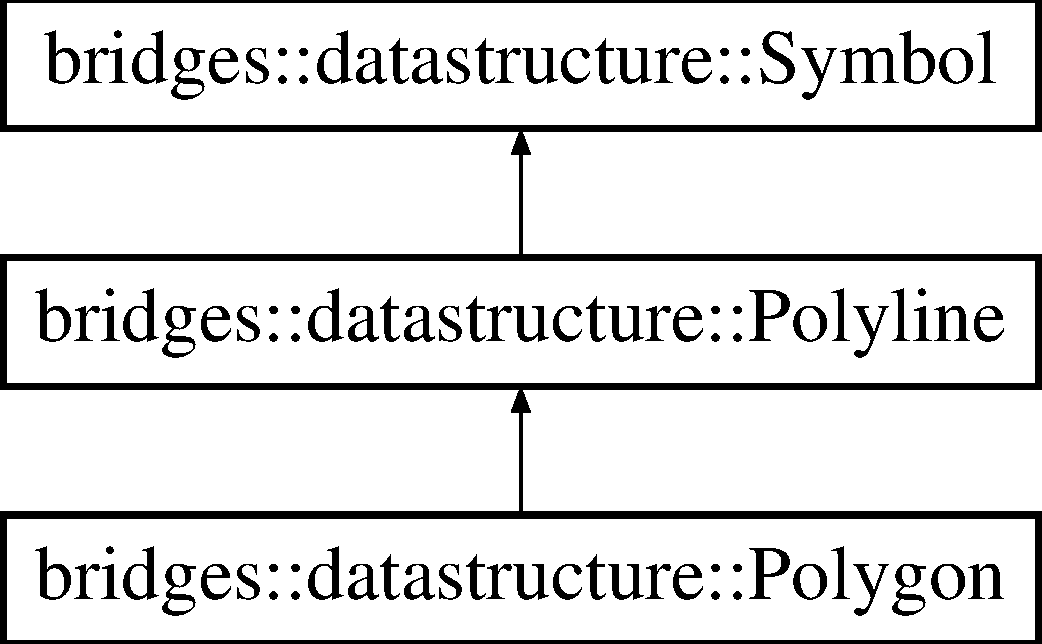
\includegraphics[height=3.000000cm]{classbridges_1_1datastructure_1_1_polygon}
\end{center}
\end{figure}


\subsection{Detailed Description}
This class defines a polygon and is part of the symbol collection. A polygon has a set of vertices, with vertices connected by line segments. It differs from the polyline in the sense that the last and first vertex are connect to close the shape. 

\begin{DoxyAuthor}{Author}
David Burlinson, Kalpathi Subramanian 
\end{DoxyAuthor}
\begin{DoxyDate}{Date}
12/23/18, 7/12/19, 12/28/20 
\end{DoxyDate}
\subsection*{Public Member Functions}
\begin{DoxyCompactItemize}
\item 
\hyperlink{classbridges_1_1datastructure_1_1_polygon_aed5756ee817adaadbff1b8e9702cbb42}{Polygon} ()
\begin{DoxyCompactList}\small\item\em default constructor \end{DoxyCompactList}\item 
\hyperlink{classbridges_1_1datastructure_1_1_polygon_a38759163e7b80c2e1582629354371ac5}{Polygon} (vector$<$ float $>$ pts)
\begin{DoxyCompactList}\small\item\em constructor, given a set of points \end{DoxyCompactList}\item 
virtual string \hyperlink{classbridges_1_1datastructure_1_1_polygon_aa5a4897e1e0818b8e786b6ddaf81230e}{get\+Data\+Struct\+Type} ()
\begin{DoxyCompactList}\small\item\em This method gets the name of the data type. \end{DoxyCompactList}\item 
virtual string \hyperlink{classbridges_1_1datastructure_1_1_polygon_a9e11131b2a1f3b6044913577f51546c3}{get\+Name} () const
\begin{DoxyCompactList}\small\item\em This method gets the name of the shape. \end{DoxyCompactList}\item 
void \hyperlink{classbridges_1_1datastructure_1_1_polygon_a058a8ec2340f15f45dab27b18978055c}{set\+Polygon} (vector$<$ float $>$ pts)
\begin{DoxyCompactList}\small\item\em constructs a polygon, given a set of points \end{DoxyCompactList}\end{DoxyCompactItemize}
\subsection*{Additional Inherited Members}


\subsection{Constructor \& Destructor Documentation}
\mbox{\Hypertarget{classbridges_1_1datastructure_1_1_polygon_aed5756ee817adaadbff1b8e9702cbb42}\label{classbridges_1_1datastructure_1_1_polygon_aed5756ee817adaadbff1b8e9702cbb42}} 
\index{bridges\+::datastructure\+::\+Polygon@{bridges\+::datastructure\+::\+Polygon}!Polygon@{Polygon}}
\index{Polygon@{Polygon}!bridges\+::datastructure\+::\+Polygon@{bridges\+::datastructure\+::\+Polygon}}
\subsubsection{\texorpdfstring{Polygon()}{Polygon()}\hspace{0.1cm}{\footnotesize\ttfamily [1/2]}}
{\footnotesize\ttfamily bridges\+::datastructure\+::\+Polygon\+::\+Polygon (\begin{DoxyParamCaption}{ }\end{DoxyParamCaption})\hspace{0.3cm}{\ttfamily [inline]}}



default constructor 

\mbox{\Hypertarget{classbridges_1_1datastructure_1_1_polygon_a38759163e7b80c2e1582629354371ac5}\label{classbridges_1_1datastructure_1_1_polygon_a38759163e7b80c2e1582629354371ac5}} 
\index{bridges\+::datastructure\+::\+Polygon@{bridges\+::datastructure\+::\+Polygon}!Polygon@{Polygon}}
\index{Polygon@{Polygon}!bridges\+::datastructure\+::\+Polygon@{bridges\+::datastructure\+::\+Polygon}}
\subsubsection{\texorpdfstring{Polygon()}{Polygon()}\hspace{0.1cm}{\footnotesize\ttfamily [2/2]}}
{\footnotesize\ttfamily bridges\+::datastructure\+::\+Polygon\+::\+Polygon (\begin{DoxyParamCaption}\item[{vector$<$ float $>$}]{pts }\end{DoxyParamCaption})\hspace{0.3cm}{\ttfamily [inline]}}



constructor, given a set of points 


\begin{DoxyParams}{Parameters}
{\em pts} & to construct polygon \\
\hline
\end{DoxyParams}


\subsection{Member Function Documentation}
\mbox{\Hypertarget{classbridges_1_1datastructure_1_1_polygon_aa5a4897e1e0818b8e786b6ddaf81230e}\label{classbridges_1_1datastructure_1_1_polygon_aa5a4897e1e0818b8e786b6ddaf81230e}} 
\index{bridges\+::datastructure\+::\+Polygon@{bridges\+::datastructure\+::\+Polygon}!get\+Data\+Struct\+Type@{get\+Data\+Struct\+Type}}
\index{get\+Data\+Struct\+Type@{get\+Data\+Struct\+Type}!bridges\+::datastructure\+::\+Polygon@{bridges\+::datastructure\+::\+Polygon}}
\subsubsection{\texorpdfstring{get\+Data\+Struct\+Type()}{getDataStructType()}}
{\footnotesize\ttfamily virtual string bridges\+::datastructure\+::\+Polygon\+::get\+Data\+Struct\+Type (\begin{DoxyParamCaption}{ }\end{DoxyParamCaption})\hspace{0.3cm}{\ttfamily [inline]}, {\ttfamily [virtual]}}



This method gets the name of the data type. 

\begin{DoxyReturn}{Returns}
name data type 
\end{DoxyReturn}
\mbox{\Hypertarget{classbridges_1_1datastructure_1_1_polygon_a9e11131b2a1f3b6044913577f51546c3}\label{classbridges_1_1datastructure_1_1_polygon_a9e11131b2a1f3b6044913577f51546c3}} 
\index{bridges\+::datastructure\+::\+Polygon@{bridges\+::datastructure\+::\+Polygon}!get\+Name@{get\+Name}}
\index{get\+Name@{get\+Name}!bridges\+::datastructure\+::\+Polygon@{bridges\+::datastructure\+::\+Polygon}}
\subsubsection{\texorpdfstring{get\+Name()}{getName()}}
{\footnotesize\ttfamily virtual string bridges\+::datastructure\+::\+Polygon\+::get\+Name (\begin{DoxyParamCaption}{ }\end{DoxyParamCaption}) const\hspace{0.3cm}{\ttfamily [inline]}, {\ttfamily [virtual]}}



This method gets the name of the shape. 

\begin{DoxyReturn}{Returns}
name shape name 
\end{DoxyReturn}
\mbox{\Hypertarget{classbridges_1_1datastructure_1_1_polygon_a058a8ec2340f15f45dab27b18978055c}\label{classbridges_1_1datastructure_1_1_polygon_a058a8ec2340f15f45dab27b18978055c}} 
\index{bridges\+::datastructure\+::\+Polygon@{bridges\+::datastructure\+::\+Polygon}!set\+Polygon@{set\+Polygon}}
\index{set\+Polygon@{set\+Polygon}!bridges\+::datastructure\+::\+Polygon@{bridges\+::datastructure\+::\+Polygon}}
\subsubsection{\texorpdfstring{set\+Polygon()}{setPolygon()}}
{\footnotesize\ttfamily void bridges\+::datastructure\+::\+Polygon\+::set\+Polygon (\begin{DoxyParamCaption}\item[{vector$<$ float $>$}]{pts }\end{DoxyParamCaption})\hspace{0.3cm}{\ttfamily [inline]}}



constructs a polygon, given a set of points 


\begin{DoxyParams}{Parameters}
{\em pts} & to construct polygon \\
\hline
\end{DoxyParams}


The documentation for this class was generated from the following file\+:\begin{DoxyCompactItemize}
\item 
/home/erik/work/bridges/bridges-\/cxx/src/\hyperlink{_polygon_8h}{Polygon.\+h}\end{DoxyCompactItemize}

\hypertarget{classbridges_1_1datastructure_1_1_polyline}{}\section{bridges\+::datastructure\+::Polyline Class Reference}
\label{classbridges_1_1datastructure_1_1_polyline}\index{bridges::datastructure::Polyline@{bridges::datastructure::Polyline}}


{\ttfamily \#include $<$Polyline.\+h$>$}

Inheritance diagram for bridges\+::datastructure\+::Polyline\+:\begin{figure}[H]
\begin{center}
\leavevmode
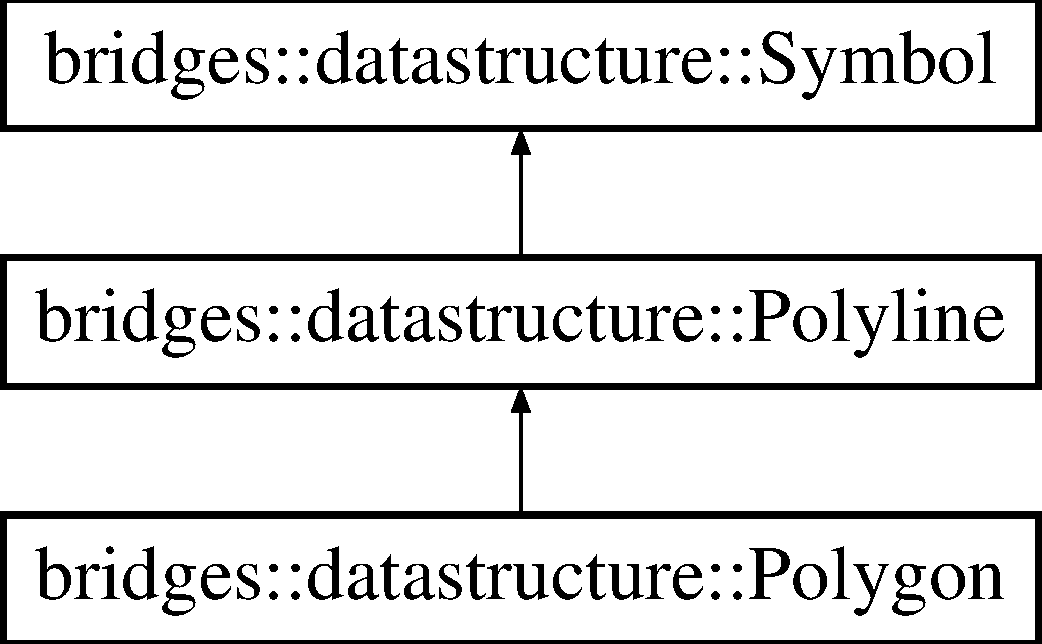
\includegraphics[height=3.000000cm]{classbridges_1_1datastructure_1_1_polyline}
\end{center}
\end{figure}


\subsection{Detailed Description}
This class defines a polyline and is part of the symbol collection. A polyline has a set of vertices with the vertices connect by line segments. 

\begin{DoxyAuthor}{Author}
David Burlinson, Kalpathi Subramanian 
\end{DoxyAuthor}
\begin{DoxyDate}{Date}
12/23/18, 7/12/19 
\end{DoxyDate}
\subsection*{Public Member Functions}
\begin{DoxyCompactItemize}
\item 
\mbox{\hyperlink{classbridges_1_1datastructure_1_1_polyline_a488f6612485fc66534035c3574281a11}{Polyline}} ()
\item 
\mbox{\hyperlink{classbridges_1_1datastructure_1_1_polyline_aceb69c3294ab4c16b2931e1073d3f996}{Polyline}} (vector$<$ float $>$ pts)
\item 
string \mbox{\hyperlink{classbridges_1_1datastructure_1_1_polyline_a49b37ad55cf64fe759ee5a0f46e2e0cc}{get\+Data\+Struct\+Type}} ()
\item 
string \mbox{\hyperlink{classbridges_1_1datastructure_1_1_polyline_a46f2830cd85a09e9c4d62d54110dbe13}{get\+Name}} () const
\item 
void \mbox{\hyperlink{classbridges_1_1datastructure_1_1_polyline_a00698223911f07cafca29ec80c507678}{add\+Point}} (float x, float y)
\item 
vector$<$ float $>$ \mbox{\hyperlink{classbridges_1_1datastructure_1_1_polyline_a634034b6874af45e2b8c56d70e8725c5}{get\+Points}} ()
\item 
void \mbox{\hyperlink{classbridges_1_1datastructure_1_1_polyline_ab1fb850dabd3ed58fd4f916992a0b9a6}{set\+Polyline}} (vector$<$ float $>$ pts)
\item 
void \mbox{\hyperlink{classbridges_1_1datastructure_1_1_polyline_a0b651b1c383b228f8d473232e64e4bda}{translate}} (float tx, float ty)
\begin{DoxyCompactList}\small\item\em Translate the polyline. \end{DoxyCompactList}\item 
void \mbox{\hyperlink{classbridges_1_1datastructure_1_1_polyline_aa61978ccbb0b086dc8f55e90ccca23c9}{rotate}} (float angle)
\item 
void \mbox{\hyperlink{classbridges_1_1datastructure_1_1_polyline_adf06f484d9a48960de84ed3646903f3a}{scale}} (float sx, float sy)
\begin{DoxyCompactList}\small\item\em Scale the polyline about its center. \end{DoxyCompactList}\item 
void \mbox{\hyperlink{classbridges_1_1datastructure_1_1_polyline_ad0783deb77873eda19528681bbbca25c}{get\+Center}} (float $\ast$center)
\item 
vector$<$ float $>$ \mbox{\hyperlink{classbridges_1_1datastructure_1_1_polyline_aebcd7f4f80e2eed35057e5b1d82ba4e7}{get\+Dimensions}} ()
\item 
const string \mbox{\hyperlink{classbridges_1_1datastructure_1_1_polyline_a176c06400a3b105fa651c69891381201}{get\+Symbol\+Representation}} () const
\end{DoxyCompactItemize}
\subsection*{Protected Attributes}
\begin{DoxyCompactItemize}
\item 
vector$<$ float $>$ \mbox{\hyperlink{classbridges_1_1datastructure_1_1_polyline_a0df21b6c3cc82930a93a495de5affda7}{points}}
\end{DoxyCompactItemize}
\subsection*{Additional Inherited Members}


\subsection{Constructor \& Destructor Documentation}
\mbox{\Hypertarget{classbridges_1_1datastructure_1_1_polyline_a488f6612485fc66534035c3574281a11}\label{classbridges_1_1datastructure_1_1_polyline_a488f6612485fc66534035c3574281a11}} 
\index{bridges::datastructure::Polyline@{bridges::datastructure::Polyline}!Polyline@{Polyline}}
\index{Polyline@{Polyline}!bridges::datastructure::Polyline@{bridges::datastructure::Polyline}}
\subsubsection{\texorpdfstring{Polyline()}{Polyline()}\hspace{0.1cm}{\footnotesize\ttfamily [1/2]}}
{\footnotesize\ttfamily bridges\+::datastructure\+::\+Polyline\+::\+Polyline (\begin{DoxyParamCaption}{ }\end{DoxyParamCaption})\hspace{0.3cm}{\ttfamily [inline]}}

\mbox{\Hypertarget{classbridges_1_1datastructure_1_1_polyline_aceb69c3294ab4c16b2931e1073d3f996}\label{classbridges_1_1datastructure_1_1_polyline_aceb69c3294ab4c16b2931e1073d3f996}} 
\index{bridges::datastructure::Polyline@{bridges::datastructure::Polyline}!Polyline@{Polyline}}
\index{Polyline@{Polyline}!bridges::datastructure::Polyline@{bridges::datastructure::Polyline}}
\subsubsection{\texorpdfstring{Polyline()}{Polyline()}\hspace{0.1cm}{\footnotesize\ttfamily [2/2]}}
{\footnotesize\ttfamily bridges\+::datastructure\+::\+Polyline\+::\+Polyline (\begin{DoxyParamCaption}\item[{vector$<$ float $>$}]{pts }\end{DoxyParamCaption})\hspace{0.3cm}{\ttfamily [inline]}}

Construct a polyline from sequence of points 
\begin{DoxyParams}{Parameters}
{\em pts} & point sequence \\
\hline
\end{DoxyParams}


\subsection{Member Function Documentation}
\mbox{\Hypertarget{classbridges_1_1datastructure_1_1_polyline_a00698223911f07cafca29ec80c507678}\label{classbridges_1_1datastructure_1_1_polyline_a00698223911f07cafca29ec80c507678}} 
\index{bridges::datastructure::Polyline@{bridges::datastructure::Polyline}!addPoint@{addPoint}}
\index{addPoint@{addPoint}!bridges::datastructure::Polyline@{bridges::datastructure::Polyline}}
\subsubsection{\texorpdfstring{addPoint()}{addPoint()}}
{\footnotesize\ttfamily void bridges\+::datastructure\+::\+Polyline\+::add\+Point (\begin{DoxyParamCaption}\item[{float}]{x,  }\item[{float}]{y }\end{DoxyParamCaption})\hspace{0.3cm}{\ttfamily [inline]}}

This method adds a point to the polyline


\begin{DoxyParams}{Parameters}
{\em x,y} & \+: X, Y coordinates of the point \\
\hline
\end{DoxyParams}
\mbox{\Hypertarget{classbridges_1_1datastructure_1_1_polyline_ad0783deb77873eda19528681bbbca25c}\label{classbridges_1_1datastructure_1_1_polyline_ad0783deb77873eda19528681bbbca25c}} 
\index{bridges::datastructure::Polyline@{bridges::datastructure::Polyline}!getCenter@{getCenter}}
\index{getCenter@{getCenter}!bridges::datastructure::Polyline@{bridges::datastructure::Polyline}}
\subsubsection{\texorpdfstring{getCenter()}{getCenter()}}
{\footnotesize\ttfamily void bridges\+::datastructure\+::\+Polyline\+::get\+Center (\begin{DoxyParamCaption}\item[{float $\ast$}]{center }\end{DoxyParamCaption})\hspace{0.3cm}{\ttfamily [inline]}}

Get center of polyline -\/ use its bounding box \mbox{\Hypertarget{classbridges_1_1datastructure_1_1_polyline_a49b37ad55cf64fe759ee5a0f46e2e0cc}\label{classbridges_1_1datastructure_1_1_polyline_a49b37ad55cf64fe759ee5a0f46e2e0cc}} 
\index{bridges::datastructure::Polyline@{bridges::datastructure::Polyline}!getDataStructType@{getDataStructType}}
\index{getDataStructType@{getDataStructType}!bridges::datastructure::Polyline@{bridges::datastructure::Polyline}}
\subsubsection{\texorpdfstring{getDataStructType()}{getDataStructType()}}
{\footnotesize\ttfamily string bridges\+::datastructure\+::\+Polyline\+::get\+Data\+Struct\+Type (\begin{DoxyParamCaption}{ }\end{DoxyParamCaption})\hspace{0.3cm}{\ttfamily [inline]}}

Get the name of the data type \begin{DoxyReturn}{Returns}
name of symbol type 
\end{DoxyReturn}
\mbox{\Hypertarget{classbridges_1_1datastructure_1_1_polyline_aebcd7f4f80e2eed35057e5b1d82ba4e7}\label{classbridges_1_1datastructure_1_1_polyline_aebcd7f4f80e2eed35057e5b1d82ba4e7}} 
\index{bridges::datastructure::Polyline@{bridges::datastructure::Polyline}!getDimensions@{getDimensions}}
\index{getDimensions@{getDimensions}!bridges::datastructure::Polyline@{bridges::datastructure::Polyline}}
\subsubsection{\texorpdfstring{getDimensions()}{getDimensions()}}
{\footnotesize\ttfamily vector$<$float$>$ bridges\+::datastructure\+::\+Polyline\+::get\+Dimensions (\begin{DoxyParamCaption}{ }\end{DoxyParamCaption})\hspace{0.3cm}{\ttfamily [inline]}, {\ttfamily [virtual]}}

This method returns the dimensions of the shape\+: min and max values in X and Y

\begin{DoxyReturn}{Returns}
array of 4 values 
\end{DoxyReturn}


Implements \mbox{\hyperlink{classbridges_1_1datastructure_1_1_symbol_a37ba60b6acdd0888677eb8c64a931679}{bridges\+::datastructure\+::\+Symbol}}.

\mbox{\Hypertarget{classbridges_1_1datastructure_1_1_polyline_a46f2830cd85a09e9c4d62d54110dbe13}\label{classbridges_1_1datastructure_1_1_polyline_a46f2830cd85a09e9c4d62d54110dbe13}} 
\index{bridges::datastructure::Polyline@{bridges::datastructure::Polyline}!getName@{getName}}
\index{getName@{getName}!bridges::datastructure::Polyline@{bridges::datastructure::Polyline}}
\subsubsection{\texorpdfstring{getName()}{getName()}}
{\footnotesize\ttfamily string bridges\+::datastructure\+::\+Polyline\+::get\+Name (\begin{DoxyParamCaption}{ }\end{DoxyParamCaption}) const\hspace{0.3cm}{\ttfamily [inline]}}

This method gets the name of the shape

\begin{DoxyReturn}{Returns}
name shape name 
\end{DoxyReturn}
\mbox{\Hypertarget{classbridges_1_1datastructure_1_1_polyline_a634034b6874af45e2b8c56d70e8725c5}\label{classbridges_1_1datastructure_1_1_polyline_a634034b6874af45e2b8c56d70e8725c5}} 
\index{bridges::datastructure::Polyline@{bridges::datastructure::Polyline}!getPoints@{getPoints}}
\index{getPoints@{getPoints}!bridges::datastructure::Polyline@{bridges::datastructure::Polyline}}
\subsubsection{\texorpdfstring{getPoints()}{getPoints()}}
{\footnotesize\ttfamily vector$<$float$>$ bridges\+::datastructure\+::\+Polyline\+::get\+Points (\begin{DoxyParamCaption}{ }\end{DoxyParamCaption})\hspace{0.3cm}{\ttfamily [inline]}}

This method returns the point list of the polyline

\begin{DoxyReturn}{Returns}
points point list of the polygon -\/ sequence of x, y values 
\end{DoxyReturn}
\mbox{\Hypertarget{classbridges_1_1datastructure_1_1_polyline_a176c06400a3b105fa651c69891381201}\label{classbridges_1_1datastructure_1_1_polyline_a176c06400a3b105fa651c69891381201}} 
\index{bridges::datastructure::Polyline@{bridges::datastructure::Polyline}!getSymbolRepresentation@{getSymbolRepresentation}}
\index{getSymbolRepresentation@{getSymbolRepresentation}!bridges::datastructure::Polyline@{bridges::datastructure::Polyline}}
\subsubsection{\texorpdfstring{getSymbolRepresentation()}{getSymbolRepresentation()}}
{\footnotesize\ttfamily const string bridges\+::datastructure\+::\+Polyline\+::get\+Symbol\+Representation (\begin{DoxyParamCaption}{ }\end{DoxyParamCaption}) const\hspace{0.3cm}{\ttfamily [inline]}, {\ttfamily [virtual]}}

This method returns the J\+S\+ON representation of the shape

\begin{DoxyReturn}{Returns}
string J\+S\+ON string 
\end{DoxyReturn}


Implements \mbox{\hyperlink{classbridges_1_1datastructure_1_1_symbol_a8044b3da559dcd9de8510ae339f126c8}{bridges\+::datastructure\+::\+Symbol}}.

\mbox{\Hypertarget{classbridges_1_1datastructure_1_1_polyline_aa61978ccbb0b086dc8f55e90ccca23c9}\label{classbridges_1_1datastructure_1_1_polyline_aa61978ccbb0b086dc8f55e90ccca23c9}} 
\index{bridges::datastructure::Polyline@{bridges::datastructure::Polyline}!rotate@{rotate}}
\index{rotate@{rotate}!bridges::datastructure::Polyline@{bridges::datastructure::Polyline}}
\subsubsection{\texorpdfstring{rotate()}{rotate()}}
{\footnotesize\ttfamily void bridges\+::datastructure\+::\+Polyline\+::rotate (\begin{DoxyParamCaption}\item[{float}]{angle }\end{DoxyParamCaption})\hspace{0.3cm}{\ttfamily [inline]}}

\begin{DoxyVerb}@brief rotate the polyline about its center
\end{DoxyVerb}
 l $\ast$ 
\begin{DoxyParams}{Parameters}
{\em angle} & rotation angle in degrees (positive is counter-\/clock wise, negative is clockwise) \\
\hline
\end{DoxyParams}
\mbox{\Hypertarget{classbridges_1_1datastructure_1_1_polyline_adf06f484d9a48960de84ed3646903f3a}\label{classbridges_1_1datastructure_1_1_polyline_adf06f484d9a48960de84ed3646903f3a}} 
\index{bridges::datastructure::Polyline@{bridges::datastructure::Polyline}!scale@{scale}}
\index{scale@{scale}!bridges::datastructure::Polyline@{bridges::datastructure::Polyline}}
\subsubsection{\texorpdfstring{scale()}{scale()}}
{\footnotesize\ttfamily void bridges\+::datastructure\+::\+Polyline\+::scale (\begin{DoxyParamCaption}\item[{float}]{sx,  }\item[{float}]{sy }\end{DoxyParamCaption})\hspace{0.3cm}{\ttfamily [inline]}}



Scale the polyline about its center. 


\begin{DoxyParams}{Parameters}
{\em sx,sy} & scale factor along each axis \\
\hline
\end{DoxyParams}
\mbox{\Hypertarget{classbridges_1_1datastructure_1_1_polyline_ab1fb850dabd3ed58fd4f916992a0b9a6}\label{classbridges_1_1datastructure_1_1_polyline_ab1fb850dabd3ed58fd4f916992a0b9a6}} 
\index{bridges::datastructure::Polyline@{bridges::datastructure::Polyline}!setPolyline@{setPolyline}}
\index{setPolyline@{setPolyline}!bridges::datastructure::Polyline@{bridges::datastructure::Polyline}}
\subsubsection{\texorpdfstring{setPolyline()}{setPolyline()}}
{\footnotesize\ttfamily void bridges\+::datastructure\+::\+Polyline\+::set\+Polyline (\begin{DoxyParamCaption}\item[{vector$<$ float $>$}]{pts }\end{DoxyParamCaption})\hspace{0.3cm}{\ttfamily [inline]}}

\mbox{\Hypertarget{classbridges_1_1datastructure_1_1_polyline_a0b651b1c383b228f8d473232e64e4bda}\label{classbridges_1_1datastructure_1_1_polyline_a0b651b1c383b228f8d473232e64e4bda}} 
\index{bridges::datastructure::Polyline@{bridges::datastructure::Polyline}!translate@{translate}}
\index{translate@{translate}!bridges::datastructure::Polyline@{bridges::datastructure::Polyline}}
\subsubsection{\texorpdfstring{translate()}{translate()}}
{\footnotesize\ttfamily void bridges\+::datastructure\+::\+Polyline\+::translate (\begin{DoxyParamCaption}\item[{float}]{tx,  }\item[{float}]{ty }\end{DoxyParamCaption})\hspace{0.3cm}{\ttfamily [inline]}}



Translate the polyline. 


\begin{DoxyParams}{Parameters}
{\em tx,ty} & translation vector \\
\hline
\end{DoxyParams}


\subsection{Member Data Documentation}
\mbox{\Hypertarget{classbridges_1_1datastructure_1_1_polyline_a0df21b6c3cc82930a93a495de5affda7}\label{classbridges_1_1datastructure_1_1_polyline_a0df21b6c3cc82930a93a495de5affda7}} 
\index{bridges::datastructure::Polyline@{bridges::datastructure::Polyline}!points@{points}}
\index{points@{points}!bridges::datastructure::Polyline@{bridges::datastructure::Polyline}}
\subsubsection{\texorpdfstring{points}{points}}
{\footnotesize\ttfamily vector$<$float$>$ bridges\+::datastructure\+::\+Polyline\+::points\hspace{0.3cm}{\ttfamily [protected]}}



The documentation for this class was generated from the following file\+:\begin{DoxyCompactItemize}
\item 
/\+Users/kalpathi/gr/bridges/cxx/src/\mbox{\hyperlink{_polyline_8h}{Polyline.\+h}}\end{DoxyCompactItemize}

\hypertarget{structrapidjson__exception}{}\section{rapidjson\+\_\+exception Struct Reference}
\label{structrapidjson__exception}\index{rapidjson\+\_\+exception@{rapidjson\+\_\+exception}}


{\ttfamily \#include $<$J\+S\+O\+Nutil.\+h$>$}

\subsection*{Public Member Functions}
\begin{DoxyCompactItemize}
\item 
\mbox{\hyperlink{structrapidjson__exception_ac81e815ea43f0364ebc365ad299584b9}{rapidjson\+\_\+exception}} (const std\+::string \&\mbox{\hyperlink{structrapidjson__exception_a6b432b89bd7052332bc923f274249e1e}{why}}, const std\+::string \&\mbox{\hyperlink{structrapidjson__exception_a56bc0e220fc6c7037e877f9f2e3f99f0}{filename}}, const int \mbox{\hyperlink{structrapidjson__exception_a9c0263f853d8a17911e29cae66708e67}{linenumber}})
\item 
\mbox{\hyperlink{structrapidjson__exception_afd42d8ce38804d2951ab8cd328cbd9e1}{operator std\+::string}} () const
\end{DoxyCompactItemize}
\subsection*{Public Attributes}
\begin{DoxyCompactItemize}
\item 
std\+::string \mbox{\hyperlink{structrapidjson__exception_a6b432b89bd7052332bc923f274249e1e}{why}}
\item 
std\+::string \mbox{\hyperlink{structrapidjson__exception_a56bc0e220fc6c7037e877f9f2e3f99f0}{filename}}
\item 
int \mbox{\hyperlink{structrapidjson__exception_a9c0263f853d8a17911e29cae66708e67}{linenumber}}
\end{DoxyCompactItemize}


\subsection{Constructor \& Destructor Documentation}
\mbox{\Hypertarget{structrapidjson__exception_ac81e815ea43f0364ebc365ad299584b9}\label{structrapidjson__exception_ac81e815ea43f0364ebc365ad299584b9}} 
\index{rapidjson\+\_\+exception@{rapidjson\+\_\+exception}!rapidjson\+\_\+exception@{rapidjson\+\_\+exception}}
\index{rapidjson\+\_\+exception@{rapidjson\+\_\+exception}!rapidjson\+\_\+exception@{rapidjson\+\_\+exception}}
\subsubsection{\texorpdfstring{rapidjson\+\_\+exception()}{rapidjson\_exception()}}
{\footnotesize\ttfamily rapidjson\+\_\+exception\+::rapidjson\+\_\+exception (\begin{DoxyParamCaption}\item[{const std\+::string \&}]{why,  }\item[{const std\+::string \&}]{filename,  }\item[{const int}]{linenumber }\end{DoxyParamCaption})\hspace{0.3cm}{\ttfamily [inline]}}



\subsection{Member Function Documentation}
\mbox{\Hypertarget{structrapidjson__exception_afd42d8ce38804d2951ab8cd328cbd9e1}\label{structrapidjson__exception_afd42d8ce38804d2951ab8cd328cbd9e1}} 
\index{rapidjson\+\_\+exception@{rapidjson\+\_\+exception}!operator std\+::string@{operator std\+::string}}
\index{operator std\+::string@{operator std\+::string}!rapidjson\+\_\+exception@{rapidjson\+\_\+exception}}
\subsubsection{\texorpdfstring{operator std\+::string()}{operator std::string()}}
{\footnotesize\ttfamily rapidjson\+\_\+exception\+::operator std\+::string (\begin{DoxyParamCaption}{ }\end{DoxyParamCaption}) const\hspace{0.3cm}{\ttfamily [inline]}}



\subsection{Member Data Documentation}
\mbox{\Hypertarget{structrapidjson__exception_a56bc0e220fc6c7037e877f9f2e3f99f0}\label{structrapidjson__exception_a56bc0e220fc6c7037e877f9f2e3f99f0}} 
\index{rapidjson\+\_\+exception@{rapidjson\+\_\+exception}!filename@{filename}}
\index{filename@{filename}!rapidjson\+\_\+exception@{rapidjson\+\_\+exception}}
\subsubsection{\texorpdfstring{filename}{filename}}
{\footnotesize\ttfamily std\+::string rapidjson\+\_\+exception\+::filename}

\mbox{\Hypertarget{structrapidjson__exception_a9c0263f853d8a17911e29cae66708e67}\label{structrapidjson__exception_a9c0263f853d8a17911e29cae66708e67}} 
\index{rapidjson\+\_\+exception@{rapidjson\+\_\+exception}!linenumber@{linenumber}}
\index{linenumber@{linenumber}!rapidjson\+\_\+exception@{rapidjson\+\_\+exception}}
\subsubsection{\texorpdfstring{linenumber}{linenumber}}
{\footnotesize\ttfamily int rapidjson\+\_\+exception\+::linenumber}

\mbox{\Hypertarget{structrapidjson__exception_a6b432b89bd7052332bc923f274249e1e}\label{structrapidjson__exception_a6b432b89bd7052332bc923f274249e1e}} 
\index{rapidjson\+\_\+exception@{rapidjson\+\_\+exception}!why@{why}}
\index{why@{why}!rapidjson\+\_\+exception@{rapidjson\+\_\+exception}}
\subsubsection{\texorpdfstring{why}{why}}
{\footnotesize\ttfamily std\+::string rapidjson\+\_\+exception\+::why}



The documentation for this struct was generated from the following file\+:\begin{DoxyCompactItemize}
\item 
/\+Users/kalpathi/gr/bridges/client/cxx/bridges18/src/\mbox{\hyperlink{_j_s_o_nutil_8h}{J\+S\+O\+Nutil.\+h}}\end{DoxyCompactItemize}

\hypertarget{classbridges_1_1datastructure_1_1_rectangle}{}\section{bridges\+:\+:datastructure\+:\+:Rectangle Class Reference}
\label{classbridges_1_1datastructure_1_1_rectangle}\index{bridges\+::datastructure\+::\+Rectangle@{bridges\+::datastructure\+::\+Rectangle}}


{\ttfamily \#include $<$Rectangle.\+h$>$}

Inheritance diagram for bridges\+:\+:datastructure\+:\+:Rectangle\+:\begin{figure}[H]
\begin{center}
\leavevmode
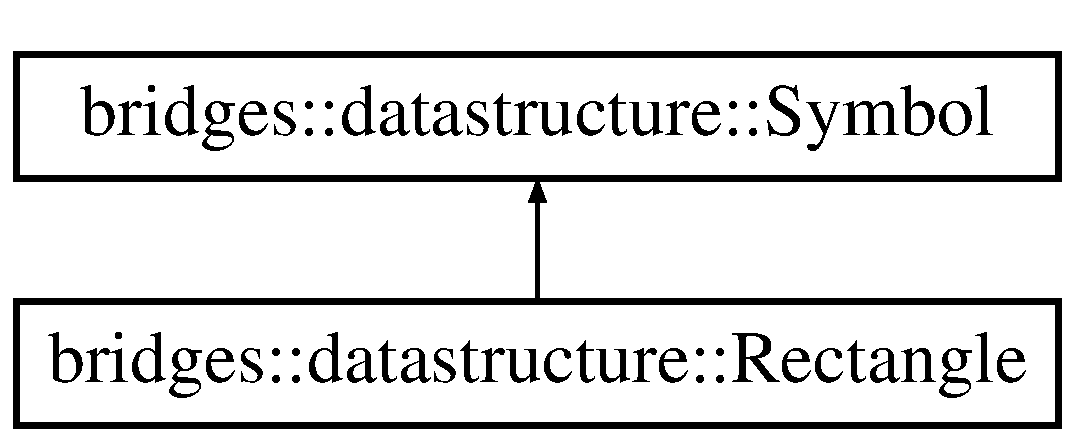
\includegraphics[height=2.000000cm]{classbridges_1_1datastructure_1_1_rectangle}
\end{center}
\end{figure}


\subsection{Detailed Description}
This class defines a rectangle and is part of the symbol collection. A rectangle has height and width. 

\begin{DoxyAuthor}{Author}
Kalpathi Subramanian 
\end{DoxyAuthor}
\begin{DoxyDate}{Date}
12/23/18, 7/12/19 
\end{DoxyDate}
\subsection*{Public Member Functions}
\begin{DoxyCompactItemize}
\item 
\hyperlink{classbridges_1_1datastructure_1_1_rectangle_a83c7e793c1335073c2a7093bbcf0c5bb}{Rectangle} ()
\begin{DoxyCompactList}\small\item\em default constructor -\/ rectangle with lower left at origin and unit length sides \end{DoxyCompactList}\item 
\hyperlink{classbridges_1_1datastructure_1_1_rectangle_a6e76090c00b4db625e96e4e23015acba}{Rectangle} (int w, int h)
\begin{DoxyCompactList}\small\item\em create rectangle with width w and height h \end{DoxyCompactList}\item 
\hyperlink{classbridges_1_1datastructure_1_1_rectangle_a8320f3a757733519e6513cdc20073e6e}{Rectangle} (float llx, float lly, float w, float h)
\begin{DoxyCompactList}\small\item\em create rectangle with width w and height h and located at given position \end{DoxyCompactList}\item 
virtual string \hyperlink{classbridges_1_1datastructure_1_1_rectangle_abb3d8cace529aae9a405909844ed1ae0}{get\+Shape\+Type} () const override
\begin{DoxyCompactList}\small\item\em This method gets the shape type name. \end{DoxyCompactList}\item 
void \hyperlink{classbridges_1_1datastructure_1_1_rectangle_a7f6182e74816a6c7cf83ae49d5ed55be}{set\+Width} (float w)
\begin{DoxyCompactList}\small\item\em This method sets the shape width. \end{DoxyCompactList}\item 
void \hyperlink{classbridges_1_1datastructure_1_1_rectangle_a6a3e99759282dd822c5615d1643f2a81}{set\+Height} (float h)
\begin{DoxyCompactList}\small\item\em This method sets the shape height. \end{DoxyCompactList}\item 
void \hyperlink{classbridges_1_1datastructure_1_1_rectangle_a931481ef10b4a7cbaca167c7d98c9467}{set\+Rectangle} (float llx, float lly, float w, float h)
\item 
virtual const string \hyperlink{classbridges_1_1datastructure_1_1_rectangle_a13fa4e45a78fdc7c49bfe566cb809ab3}{get\+Symbol\+Representation} () const override
\begin{DoxyCompactList}\small\item\em This method returns the J\+S\+ON representation of the shape. \end{DoxyCompactList}\end{DoxyCompactItemize}
\subsection*{Additional Inherited Members}


\subsection{Constructor \& Destructor Documentation}
\mbox{\Hypertarget{classbridges_1_1datastructure_1_1_rectangle_a83c7e793c1335073c2a7093bbcf0c5bb}\label{classbridges_1_1datastructure_1_1_rectangle_a83c7e793c1335073c2a7093bbcf0c5bb}} 
\index{bridges\+::datastructure\+::\+Rectangle@{bridges\+::datastructure\+::\+Rectangle}!Rectangle@{Rectangle}}
\index{Rectangle@{Rectangle}!bridges\+::datastructure\+::\+Rectangle@{bridges\+::datastructure\+::\+Rectangle}}
\subsubsection{\texorpdfstring{Rectangle()}{Rectangle()}\hspace{0.1cm}{\footnotesize\ttfamily [1/3]}}
{\footnotesize\ttfamily bridges\+::datastructure\+::\+Rectangle\+::\+Rectangle (\begin{DoxyParamCaption}{ }\end{DoxyParamCaption})\hspace{0.3cm}{\ttfamily [inline]}}



default constructor -\/ rectangle with lower left at origin and unit length sides 

\mbox{\Hypertarget{classbridges_1_1datastructure_1_1_rectangle_a6e76090c00b4db625e96e4e23015acba}\label{classbridges_1_1datastructure_1_1_rectangle_a6e76090c00b4db625e96e4e23015acba}} 
\index{bridges\+::datastructure\+::\+Rectangle@{bridges\+::datastructure\+::\+Rectangle}!Rectangle@{Rectangle}}
\index{Rectangle@{Rectangle}!bridges\+::datastructure\+::\+Rectangle@{bridges\+::datastructure\+::\+Rectangle}}
\subsubsection{\texorpdfstring{Rectangle()}{Rectangle()}\hspace{0.1cm}{\footnotesize\ttfamily [2/3]}}
{\footnotesize\ttfamily bridges\+::datastructure\+::\+Rectangle\+::\+Rectangle (\begin{DoxyParamCaption}\item[{int}]{w,  }\item[{int}]{h }\end{DoxyParamCaption})\hspace{0.3cm}{\ttfamily [inline]}}



create rectangle with width w and height h 


\begin{DoxyParams}{Parameters}
{\em w} & width \\
\hline
{\em h} & height \\
\hline
\end{DoxyParams}
\mbox{\Hypertarget{classbridges_1_1datastructure_1_1_rectangle_a8320f3a757733519e6513cdc20073e6e}\label{classbridges_1_1datastructure_1_1_rectangle_a8320f3a757733519e6513cdc20073e6e}} 
\index{bridges\+::datastructure\+::\+Rectangle@{bridges\+::datastructure\+::\+Rectangle}!Rectangle@{Rectangle}}
\index{Rectangle@{Rectangle}!bridges\+::datastructure\+::\+Rectangle@{bridges\+::datastructure\+::\+Rectangle}}
\subsubsection{\texorpdfstring{Rectangle()}{Rectangle()}\hspace{0.1cm}{\footnotesize\ttfamily [3/3]}}
{\footnotesize\ttfamily bridges\+::datastructure\+::\+Rectangle\+::\+Rectangle (\begin{DoxyParamCaption}\item[{float}]{llx,  }\item[{float}]{lly,  }\item[{float}]{w,  }\item[{float}]{h }\end{DoxyParamCaption})\hspace{0.3cm}{\ttfamily [inline]}}



create rectangle with width w and height h and located at given position 


\begin{DoxyParams}{Parameters}
{\em locx} & rect lower left -\/ x coord \\
\hline
{\em locy} & rect lower left -\/ y coord \\
\hline
{\em w} & width \\
\hline
{\em h} & height \\
\hline
\end{DoxyParams}


\subsection{Member Function Documentation}
\mbox{\Hypertarget{classbridges_1_1datastructure_1_1_rectangle_abb3d8cace529aae9a405909844ed1ae0}\label{classbridges_1_1datastructure_1_1_rectangle_abb3d8cace529aae9a405909844ed1ae0}} 
\index{bridges\+::datastructure\+::\+Rectangle@{bridges\+::datastructure\+::\+Rectangle}!get\+Shape\+Type@{get\+Shape\+Type}}
\index{get\+Shape\+Type@{get\+Shape\+Type}!bridges\+::datastructure\+::\+Rectangle@{bridges\+::datastructure\+::\+Rectangle}}
\subsubsection{\texorpdfstring{get\+Shape\+Type()}{getShapeType()}}
{\footnotesize\ttfamily virtual string bridges\+::datastructure\+::\+Rectangle\+::get\+Shape\+Type (\begin{DoxyParamCaption}{ }\end{DoxyParamCaption}) const\hspace{0.3cm}{\ttfamily [inline]}, {\ttfamily [override]}, {\ttfamily [virtual]}}



This method gets the shape type name. 

\begin{DoxyReturn}{Returns}
shape type 
\end{DoxyReturn}


Implements \hyperlink{classbridges_1_1datastructure_1_1_symbol_a1fb7cabce2915b103b8474658e8549f8}{bridges\+::datastructure\+::\+Symbol}.

\mbox{\Hypertarget{classbridges_1_1datastructure_1_1_rectangle_a13fa4e45a78fdc7c49bfe566cb809ab3}\label{classbridges_1_1datastructure_1_1_rectangle_a13fa4e45a78fdc7c49bfe566cb809ab3}} 
\index{bridges\+::datastructure\+::\+Rectangle@{bridges\+::datastructure\+::\+Rectangle}!get\+Symbol\+Representation@{get\+Symbol\+Representation}}
\index{get\+Symbol\+Representation@{get\+Symbol\+Representation}!bridges\+::datastructure\+::\+Rectangle@{bridges\+::datastructure\+::\+Rectangle}}
\subsubsection{\texorpdfstring{get\+Symbol\+Representation()}{getSymbolRepresentation()}}
{\footnotesize\ttfamily virtual const string bridges\+::datastructure\+::\+Rectangle\+::get\+Symbol\+Representation (\begin{DoxyParamCaption}{ }\end{DoxyParamCaption}) const\hspace{0.3cm}{\ttfamily [inline]}, {\ttfamily [override]}, {\ttfamily [virtual]}}



This method returns the J\+S\+ON representation of the shape. 

\begin{DoxyReturn}{Returns}
string J\+S\+ON string 
\end{DoxyReturn}


Implements \hyperlink{classbridges_1_1datastructure_1_1_symbol_a8044b3da559dcd9de8510ae339f126c8}{bridges\+::datastructure\+::\+Symbol}.

\mbox{\Hypertarget{classbridges_1_1datastructure_1_1_rectangle_a6a3e99759282dd822c5615d1643f2a81}\label{classbridges_1_1datastructure_1_1_rectangle_a6a3e99759282dd822c5615d1643f2a81}} 
\index{bridges\+::datastructure\+::\+Rectangle@{bridges\+::datastructure\+::\+Rectangle}!set\+Height@{set\+Height}}
\index{set\+Height@{set\+Height}!bridges\+::datastructure\+::\+Rectangle@{bridges\+::datastructure\+::\+Rectangle}}
\subsubsection{\texorpdfstring{set\+Height()}{setHeight()}}
{\footnotesize\ttfamily void bridges\+::datastructure\+::\+Rectangle\+::set\+Height (\begin{DoxyParamCaption}\item[{float}]{h }\end{DoxyParamCaption})\hspace{0.3cm}{\ttfamily [inline]}}



This method sets the shape height. 


\begin{DoxyParams}{Parameters}
{\em h} & height \\
\hline
\end{DoxyParams}
\mbox{\Hypertarget{classbridges_1_1datastructure_1_1_rectangle_a931481ef10b4a7cbaca167c7d98c9467}\label{classbridges_1_1datastructure_1_1_rectangle_a931481ef10b4a7cbaca167c7d98c9467}} 
\index{bridges\+::datastructure\+::\+Rectangle@{bridges\+::datastructure\+::\+Rectangle}!set\+Rectangle@{set\+Rectangle}}
\index{set\+Rectangle@{set\+Rectangle}!bridges\+::datastructure\+::\+Rectangle@{bridges\+::datastructure\+::\+Rectangle}}
\subsubsection{\texorpdfstring{set\+Rectangle()}{setRectangle()}}
{\footnotesize\ttfamily void bridges\+::datastructure\+::\+Rectangle\+::set\+Rectangle (\begin{DoxyParamCaption}\item[{float}]{llx,  }\item[{float}]{lly,  }\item[{float}]{w,  }\item[{float}]{h }\end{DoxyParamCaption})\hspace{0.3cm}{\ttfamily [inline]}}

\mbox{\Hypertarget{classbridges_1_1datastructure_1_1_rectangle_a7f6182e74816a6c7cf83ae49d5ed55be}\label{classbridges_1_1datastructure_1_1_rectangle_a7f6182e74816a6c7cf83ae49d5ed55be}} 
\index{bridges\+::datastructure\+::\+Rectangle@{bridges\+::datastructure\+::\+Rectangle}!set\+Width@{set\+Width}}
\index{set\+Width@{set\+Width}!bridges\+::datastructure\+::\+Rectangle@{bridges\+::datastructure\+::\+Rectangle}}
\subsubsection{\texorpdfstring{set\+Width()}{setWidth()}}
{\footnotesize\ttfamily void bridges\+::datastructure\+::\+Rectangle\+::set\+Width (\begin{DoxyParamCaption}\item[{float}]{w }\end{DoxyParamCaption})\hspace{0.3cm}{\ttfamily [inline]}}



This method sets the shape width. 


\begin{DoxyParams}{Parameters}
{\em w} & width \\
\hline
\end{DoxyParams}


The documentation for this class was generated from the following file\+:\begin{DoxyCompactItemize}
\item 
/home/erik/work/bridges/bridges-\/cxx/src/\hyperlink{_rectangle_8h}{Rectangle.\+h}\end{DoxyCompactItemize}

\hypertarget{classbridges_1_1_server_comm}{}\section{bridges\+:\+:Server\+Comm Class Reference}
\label{classbridges_1_1_server_comm}\index{bridges\+::\+Server\+Comm@{bridges\+::\+Server\+Comm}}


This is a detail class for the \mbox{\hyperlink{classbridges_1_1_bridges}{Bridges}} namespace and is not intended for external use.  




{\ttfamily \#include $<$Server\+Comm.\+h$>$}

\subsection*{Friends}
\begin{DoxyCompactItemize}
\item 
class \mbox{\hyperlink{classbridges_1_1_server_comm_a1e7012f84e4df45aa77f36ad8d8375eb}{Bridges}}
\item 
class \mbox{\hyperlink{classbridges_1_1_server_comm_a7998ddaa8bd7c3b9a7cd2a8cbf3573c4}{Data\+Source}}
\end{DoxyCompactItemize}


\subsection{Detailed Description}
This is a detail class for the \mbox{\hyperlink{classbridges_1_1_bridges}{Bridges}} namespace and is not intended for external use. 

\subsection{Friends And Related Function Documentation}
\mbox{\Hypertarget{classbridges_1_1_server_comm_a1e7012f84e4df45aa77f36ad8d8375eb}\label{classbridges_1_1_server_comm_a1e7012f84e4df45aa77f36ad8d8375eb}} 
\index{bridges\+::\+Server\+Comm@{bridges\+::\+Server\+Comm}!Bridges@{Bridges}}
\index{Bridges@{Bridges}!bridges\+::\+Server\+Comm@{bridges\+::\+Server\+Comm}}
\subsubsection{\texorpdfstring{Bridges}{Bridges}}
{\footnotesize\ttfamily friend class \mbox{\hyperlink{classbridges_1_1_bridges}{Bridges}}\hspace{0.3cm}{\ttfamily [friend]}}

\mbox{\Hypertarget{classbridges_1_1_server_comm_a7998ddaa8bd7c3b9a7cd2a8cbf3573c4}\label{classbridges_1_1_server_comm_a7998ddaa8bd7c3b9a7cd2a8cbf3573c4}} 
\index{bridges\+::\+Server\+Comm@{bridges\+::\+Server\+Comm}!Data\+Source@{Data\+Source}}
\index{Data\+Source@{Data\+Source}!bridges\+::\+Server\+Comm@{bridges\+::\+Server\+Comm}}
\subsubsection{\texorpdfstring{Data\+Source}{DataSource}}
{\footnotesize\ttfamily friend class \mbox{\hyperlink{classbridges_1_1_data_source}{Data\+Source}}\hspace{0.3cm}{\ttfamily [friend]}}



The documentation for this class was generated from the following file\+:\begin{DoxyCompactItemize}
\item 
/\+Users/kalpathi/gr/bridges/client/cxx/bridges18/src/\mbox{\hyperlink{_server_comm_8h}{Server\+Comm.\+h}}\end{DoxyCompactItemize}

\hypertarget{classbridges_1_1dataset_1_1_shakespeare}{}\section{bridges\+:\+:dataset\+:\+:Shakespeare Class Reference}
\label{classbridges_1_1dataset_1_1_shakespeare}\index{bridges\+::dataset\+::\+Shakespeare@{bridges\+::dataset\+::\+Shakespeare}}


{\ttfamily \#include $<$Shakespeare.\+h$>$}



\subsection{Detailed Description}
A \hyperlink{classbridges_1_1dataset_1_1_shakespeare}{Shakespeare} Data source object containing sonnets, poems and plays. 

This is a convenience class provided for users who wish to use this data source as part of their application. It provides an A\+PI that makes it easy to access the attributes of this data set.

Refer to tutorial examples to using this data source in data structure assignments.

Refer to tutorial examples to using this data source in data structure assignments.

\begin{DoxyAuthor}{Author}
Kalpathi Subramanian 
\end{DoxyAuthor}
\begin{DoxyDate}{Date}
1/16/17, 12/28/20 
\end{DoxyDate}
\subsection*{Public Member Functions}
\begin{DoxyCompactItemize}
\item 
\hyperlink{classbridges_1_1dataset_1_1_shakespeare_a58ff458b70e8198b2e235eacd17be91c}{Shakespeare} ()
\item 
\hyperlink{classbridges_1_1dataset_1_1_shakespeare_a859f3625fb8019967aa8083f20993cad}{Shakespeare} (const string \&title, const string \&type, const string \&text)
\item 
string \hyperlink{classbridges_1_1dataset_1_1_shakespeare_a00ff743145899bf88435b194b6291ce7}{get\+Title} () const
\item 
void \hyperlink{classbridges_1_1dataset_1_1_shakespeare_a92c11a229b38913fea73cfe26474587b}{set\+Title} (const string \&title)
\item 
string \hyperlink{classbridges_1_1dataset_1_1_shakespeare_af0cc6fd91d90e663d343c52756e9f191}{get\+Type} () const
\item 
void \hyperlink{classbridges_1_1dataset_1_1_shakespeare_a4e9d1126524d2b10f5fe36ffd4588f15}{set\+Type} (const string \&type)
\item 
string \hyperlink{classbridges_1_1dataset_1_1_shakespeare_a23de5e2229cc15bb1c9f1eacaee007ee}{get\+Text} () const
\item 
void \hyperlink{classbridges_1_1dataset_1_1_shakespeare_af285363fb2bfe9cf302786ae31d4cc8c}{set\+Text} (const string \&text)
\end{DoxyCompactItemize}


\subsection{Constructor \& Destructor Documentation}
\mbox{\Hypertarget{classbridges_1_1dataset_1_1_shakespeare_a58ff458b70e8198b2e235eacd17be91c}\label{classbridges_1_1dataset_1_1_shakespeare_a58ff458b70e8198b2e235eacd17be91c}} 
\index{bridges\+::dataset\+::\+Shakespeare@{bridges\+::dataset\+::\+Shakespeare}!Shakespeare@{Shakespeare}}
\index{Shakespeare@{Shakespeare}!bridges\+::dataset\+::\+Shakespeare@{bridges\+::dataset\+::\+Shakespeare}}
\subsubsection{\texorpdfstring{Shakespeare()}{Shakespeare()}\hspace{0.1cm}{\footnotesize\ttfamily [1/2]}}
{\footnotesize\ttfamily bridges\+::dataset\+::\+Shakespeare\+::\+Shakespeare (\begin{DoxyParamCaption}{ }\end{DoxyParamCaption})\hspace{0.3cm}{\ttfamily [inline]}}

Constructor \mbox{\Hypertarget{classbridges_1_1dataset_1_1_shakespeare_a859f3625fb8019967aa8083f20993cad}\label{classbridges_1_1dataset_1_1_shakespeare_a859f3625fb8019967aa8083f20993cad}} 
\index{bridges\+::dataset\+::\+Shakespeare@{bridges\+::dataset\+::\+Shakespeare}!Shakespeare@{Shakespeare}}
\index{Shakespeare@{Shakespeare}!bridges\+::dataset\+::\+Shakespeare@{bridges\+::dataset\+::\+Shakespeare}}
\subsubsection{\texorpdfstring{Shakespeare()}{Shakespeare()}\hspace{0.1cm}{\footnotesize\ttfamily [2/2]}}
{\footnotesize\ttfamily bridges\+::dataset\+::\+Shakespeare\+::\+Shakespeare (\begin{DoxyParamCaption}\item[{const string \&}]{title,  }\item[{const string \&}]{type,  }\item[{const string \&}]{text }\end{DoxyParamCaption})\hspace{0.3cm}{\ttfamily [inline]}}

Constructor


\begin{DoxyParams}{Parameters}
{\em title} & title of sonnet, play or poem \\
\hline
{\em type} & (sonnet, play or poem) \\
\hline
{\em text} & full text of entity \\
\hline
\end{DoxyParams}


\subsection{Member Function Documentation}
\mbox{\Hypertarget{classbridges_1_1dataset_1_1_shakespeare_a23de5e2229cc15bb1c9f1eacaee007ee}\label{classbridges_1_1dataset_1_1_shakespeare_a23de5e2229cc15bb1c9f1eacaee007ee}} 
\index{bridges\+::dataset\+::\+Shakespeare@{bridges\+::dataset\+::\+Shakespeare}!get\+Text@{get\+Text}}
\index{get\+Text@{get\+Text}!bridges\+::dataset\+::\+Shakespeare@{bridges\+::dataset\+::\+Shakespeare}}
\subsubsection{\texorpdfstring{get\+Text()}{getText()}}
{\footnotesize\ttfamily string bridges\+::dataset\+::\+Shakespeare\+::get\+Text (\begin{DoxyParamCaption}{ }\end{DoxyParamCaption}) const\hspace{0.3cm}{\ttfamily [inline]}}

Get full text of sonnet, play or poem \begin{DoxyReturn}{Returns}
full text (string) 
\end{DoxyReturn}
\mbox{\Hypertarget{classbridges_1_1dataset_1_1_shakespeare_a00ff743145899bf88435b194b6291ce7}\label{classbridges_1_1dataset_1_1_shakespeare_a00ff743145899bf88435b194b6291ce7}} 
\index{bridges\+::dataset\+::\+Shakespeare@{bridges\+::dataset\+::\+Shakespeare}!get\+Title@{get\+Title}}
\index{get\+Title@{get\+Title}!bridges\+::dataset\+::\+Shakespeare@{bridges\+::dataset\+::\+Shakespeare}}
\subsubsection{\texorpdfstring{get\+Title()}{getTitle()}}
{\footnotesize\ttfamily string bridges\+::dataset\+::\+Shakespeare\+::get\+Title (\begin{DoxyParamCaption}{ }\end{DoxyParamCaption}) const\hspace{0.3cm}{\ttfamily [inline]}}

Get title of sonnet, play or poem \begin{DoxyReturn}{Returns}
title (string) 
\end{DoxyReturn}
\mbox{\Hypertarget{classbridges_1_1dataset_1_1_shakespeare_af0cc6fd91d90e663d343c52756e9f191}\label{classbridges_1_1dataset_1_1_shakespeare_af0cc6fd91d90e663d343c52756e9f191}} 
\index{bridges\+::dataset\+::\+Shakespeare@{bridges\+::dataset\+::\+Shakespeare}!get\+Type@{get\+Type}}
\index{get\+Type@{get\+Type}!bridges\+::dataset\+::\+Shakespeare@{bridges\+::dataset\+::\+Shakespeare}}
\subsubsection{\texorpdfstring{get\+Type()}{getType()}}
{\footnotesize\ttfamily string bridges\+::dataset\+::\+Shakespeare\+::get\+Type (\begin{DoxyParamCaption}{ }\end{DoxyParamCaption}) const\hspace{0.3cm}{\ttfamily [inline]}}

Get type of sonnet, play or poem \begin{DoxyReturn}{Returns}
type (string) 
\end{DoxyReturn}
\mbox{\Hypertarget{classbridges_1_1dataset_1_1_shakespeare_af285363fb2bfe9cf302786ae31d4cc8c}\label{classbridges_1_1dataset_1_1_shakespeare_af285363fb2bfe9cf302786ae31d4cc8c}} 
\index{bridges\+::dataset\+::\+Shakespeare@{bridges\+::dataset\+::\+Shakespeare}!set\+Text@{set\+Text}}
\index{set\+Text@{set\+Text}!bridges\+::dataset\+::\+Shakespeare@{bridges\+::dataset\+::\+Shakespeare}}
\subsubsection{\texorpdfstring{set\+Text()}{setText()}}
{\footnotesize\ttfamily void bridges\+::dataset\+::\+Shakespeare\+::set\+Text (\begin{DoxyParamCaption}\item[{const string \&}]{text }\end{DoxyParamCaption})\hspace{0.3cm}{\ttfamily [inline]}}

set full text of sonnet, play or poem 
\begin{DoxyParams}{Parameters}
{\em text} & full text (string) to be set \\
\hline
\end{DoxyParams}
\mbox{\Hypertarget{classbridges_1_1dataset_1_1_shakespeare_a92c11a229b38913fea73cfe26474587b}\label{classbridges_1_1dataset_1_1_shakespeare_a92c11a229b38913fea73cfe26474587b}} 
\index{bridges\+::dataset\+::\+Shakespeare@{bridges\+::dataset\+::\+Shakespeare}!set\+Title@{set\+Title}}
\index{set\+Title@{set\+Title}!bridges\+::dataset\+::\+Shakespeare@{bridges\+::dataset\+::\+Shakespeare}}
\subsubsection{\texorpdfstring{set\+Title()}{setTitle()}}
{\footnotesize\ttfamily void bridges\+::dataset\+::\+Shakespeare\+::set\+Title (\begin{DoxyParamCaption}\item[{const string \&}]{title }\end{DoxyParamCaption})\hspace{0.3cm}{\ttfamily [inline]}}

set title of sonnet, play or poem 
\begin{DoxyParams}{Parameters}
{\em title} & (string) to be set \\
\hline
\end{DoxyParams}
\mbox{\Hypertarget{classbridges_1_1dataset_1_1_shakespeare_a4e9d1126524d2b10f5fe36ffd4588f15}\label{classbridges_1_1dataset_1_1_shakespeare_a4e9d1126524d2b10f5fe36ffd4588f15}} 
\index{bridges\+::dataset\+::\+Shakespeare@{bridges\+::dataset\+::\+Shakespeare}!set\+Type@{set\+Type}}
\index{set\+Type@{set\+Type}!bridges\+::dataset\+::\+Shakespeare@{bridges\+::dataset\+::\+Shakespeare}}
\subsubsection{\texorpdfstring{set\+Type()}{setType()}}
{\footnotesize\ttfamily void bridges\+::dataset\+::\+Shakespeare\+::set\+Type (\begin{DoxyParamCaption}\item[{const string \&}]{type }\end{DoxyParamCaption})\hspace{0.3cm}{\ttfamily [inline]}}

set type to sonnet, play or poem 
\begin{DoxyParams}{Parameters}
{\em type} & (string) to be set \\
\hline
\end{DoxyParams}


The documentation for this class was generated from the following file\+:\begin{DoxyCompactItemize}
\item 
/home/erik/work/bridges/bridges-\/cxx/src/data\+\_\+src/\hyperlink{_shakespeare_8h}{Shakespeare.\+h}\end{DoxyCompactItemize}

\hypertarget{classbridges_1_1benchmark_1_1_shortest_path_benchmark}{}\section{bridges.\+benchmark.\+Shortest\+Path\+Benchmark Class Reference}
\label{classbridges_1_1benchmark_1_1_shortest_path_benchmark}\index{bridges.\+benchmark.\+Shortest\+Path\+Benchmark@{bridges.\+benchmark.\+Shortest\+Path\+Benchmark}}


Inherits bridges.\+benchmark.\+Graph\+Benchmark.



\subsection{Detailed Description}
Benchmarks Shortest Path algorithms. 

Benchmarks Shortest Path algorithms and add time series to a Line\+Chart.

One can also set a maximum time spent on a particular run using set\+Time\+Cap();

and can be passed to the run function for being benchmarked. A typical use would look something like


\begin{DoxyCode}
LineChart lc;
\mbox{\hyperlink{classbridges_1_1benchmark_1_1_shortest_path_benchmark_ad878c2ad9c6912170601092423c54c43}{ShortestPathBenchmark}} sb = \textcolor{keyword}{new} \mbox{\hyperlink{classbridges_1_1benchmark_1_1_shortest_path_benchmark_ad878c2ad9c6912170601092423c54c43}{ShortestPathBenchmark}}(lc);
sb.run(\textcolor{stringliteral}{"mybfsalgorithm"}, spalgo);
\end{DoxyCode}


\begin{DoxyAuthor}{Author}
Erik Saule 
\end{DoxyAuthor}
\begin{DoxyDate}{Date}
07/21/2019 
\end{DoxyDate}
\subsection*{Public Member Functions}
\begin{DoxyCompactItemize}
\item 
\mbox{\hyperlink{classbridges_1_1benchmark_1_1_shortest_path_benchmark_ad878c2ad9c6912170601092423c54c43}{Shortest\+Path\+Benchmark}} (\mbox{\hyperlink{classbridges_1_1base_1_1_line_chart}{Line\+Chart}} plot, long time\+Cap)
\item 
\mbox{\hyperlink{classbridges_1_1benchmark_1_1_shortest_path_benchmark_ac84a2afc6e663b9d4edc61b3d4c4701c}{Shortest\+Path\+Benchmark}} (\mbox{\hyperlink{classbridges_1_1base_1_1_line_chart}{Line\+Chart}} plot)
\item 
void \mbox{\hyperlink{classbridges_1_1benchmark_1_1_shortest_path_benchmark_ad7e6918e142cfbdaac08493ccbf02acf}{run}} (String algo\+Name, Consumer$<$ \mbox{\hyperlink{classbridges_1_1benchmark_1_1_shortest_path_params}{Shortest\+Path\+Params}} $>$ sp\+Algo)  throws I\+O\+Exception 
\begin{DoxyCompactList}\small\item\em benchmark a particular Shortest Path algorithm that accepts a single \mbox{\hyperlink{classbridges_1_1benchmark_1_1_shortest_path_params}{Shortest\+Path\+Params}} argument \end{DoxyCompactList}\end{DoxyCompactItemize}


\subsection{Constructor \& Destructor Documentation}
\mbox{\Hypertarget{classbridges_1_1benchmark_1_1_shortest_path_benchmark_ad878c2ad9c6912170601092423c54c43}\label{classbridges_1_1benchmark_1_1_shortest_path_benchmark_ad878c2ad9c6912170601092423c54c43}} 
\index{bridges\+::benchmark\+::\+Shortest\+Path\+Benchmark@{bridges\+::benchmark\+::\+Shortest\+Path\+Benchmark}!Shortest\+Path\+Benchmark@{Shortest\+Path\+Benchmark}}
\index{Shortest\+Path\+Benchmark@{Shortest\+Path\+Benchmark}!bridges\+::benchmark\+::\+Shortest\+Path\+Benchmark@{bridges\+::benchmark\+::\+Shortest\+Path\+Benchmark}}
\subsubsection{\texorpdfstring{Shortest\+Path\+Benchmark()}{ShortestPathBenchmark()}\hspace{0.1cm}{\footnotesize\ttfamily [1/2]}}
{\footnotesize\ttfamily bridges.\+benchmark.\+Shortest\+Path\+Benchmark.\+Shortest\+Path\+Benchmark (\begin{DoxyParamCaption}\item[{\mbox{\hyperlink{classbridges_1_1base_1_1_line_chart}{Line\+Chart}}}]{plot,  }\item[{long}]{time\+Cap }\end{DoxyParamCaption})}

\mbox{\Hypertarget{classbridges_1_1benchmark_1_1_shortest_path_benchmark_ac84a2afc6e663b9d4edc61b3d4c4701c}\label{classbridges_1_1benchmark_1_1_shortest_path_benchmark_ac84a2afc6e663b9d4edc61b3d4c4701c}} 
\index{bridges\+::benchmark\+::\+Shortest\+Path\+Benchmark@{bridges\+::benchmark\+::\+Shortest\+Path\+Benchmark}!Shortest\+Path\+Benchmark@{Shortest\+Path\+Benchmark}}
\index{Shortest\+Path\+Benchmark@{Shortest\+Path\+Benchmark}!bridges\+::benchmark\+::\+Shortest\+Path\+Benchmark@{bridges\+::benchmark\+::\+Shortest\+Path\+Benchmark}}
\subsubsection{\texorpdfstring{Shortest\+Path\+Benchmark()}{ShortestPathBenchmark()}\hspace{0.1cm}{\footnotesize\ttfamily [2/2]}}
{\footnotesize\ttfamily bridges.\+benchmark.\+Shortest\+Path\+Benchmark.\+Shortest\+Path\+Benchmark (\begin{DoxyParamCaption}\item[{\mbox{\hyperlink{classbridges_1_1base_1_1_line_chart}{Line\+Chart}}}]{plot }\end{DoxyParamCaption})}



\subsection{Member Function Documentation}
\mbox{\Hypertarget{classbridges_1_1benchmark_1_1_shortest_path_benchmark_ad7e6918e142cfbdaac08493ccbf02acf}\label{classbridges_1_1benchmark_1_1_shortest_path_benchmark_ad7e6918e142cfbdaac08493ccbf02acf}} 
\index{bridges\+::benchmark\+::\+Shortest\+Path\+Benchmark@{bridges\+::benchmark\+::\+Shortest\+Path\+Benchmark}!run@{run}}
\index{run@{run}!bridges\+::benchmark\+::\+Shortest\+Path\+Benchmark@{bridges\+::benchmark\+::\+Shortest\+Path\+Benchmark}}
\subsubsection{\texorpdfstring{run()}{run()}}
{\footnotesize\ttfamily void bridges.\+benchmark.\+Shortest\+Path\+Benchmark.\+run (\begin{DoxyParamCaption}\item[{String}]{algo\+Name,  }\item[{Consumer$<$ \mbox{\hyperlink{classbridges_1_1benchmark_1_1_shortest_path_params}{Shortest\+Path\+Params}} $>$}]{sp\+Algo }\end{DoxyParamCaption}) throws I\+O\+Exception}



benchmark a particular Shortest Path algorithm that accepts a single \mbox{\hyperlink{classbridges_1_1benchmark_1_1_shortest_path_params}{Shortest\+Path\+Params}} argument 


\begin{DoxyParams}{Parameters}
{\em algo\+Name} & Screen name of the algorithm \\
\hline
{\em sp\+Algo} & the actual algorithm \\
\hline
\end{DoxyParams}


The documentation for this class was generated from the following file\+:\begin{DoxyCompactItemize}
\item 
/\+Users/kalpathi/gr/bridges/client/java/src/main/java/bridges/benchmark/\mbox{\hyperlink{_shortest_path_benchmark_8java}{Shortest\+Path\+Benchmark.\+java}}\end{DoxyCompactItemize}

\hypertarget{classbridges_1_1_simple_cache}{}\section{bridges\+:\+:Simple\+Cache Class Reference}
\label{classbridges_1_1_simple_cache}\index{bridges\+::\+Simple\+Cache@{bridges\+::\+Simple\+Cache}}


{\ttfamily \#include $<$Cache.\+h$>$}

Inheritance diagram for bridges\+:\+:Simple\+Cache\+:\begin{figure}[H]
\begin{center}
\leavevmode
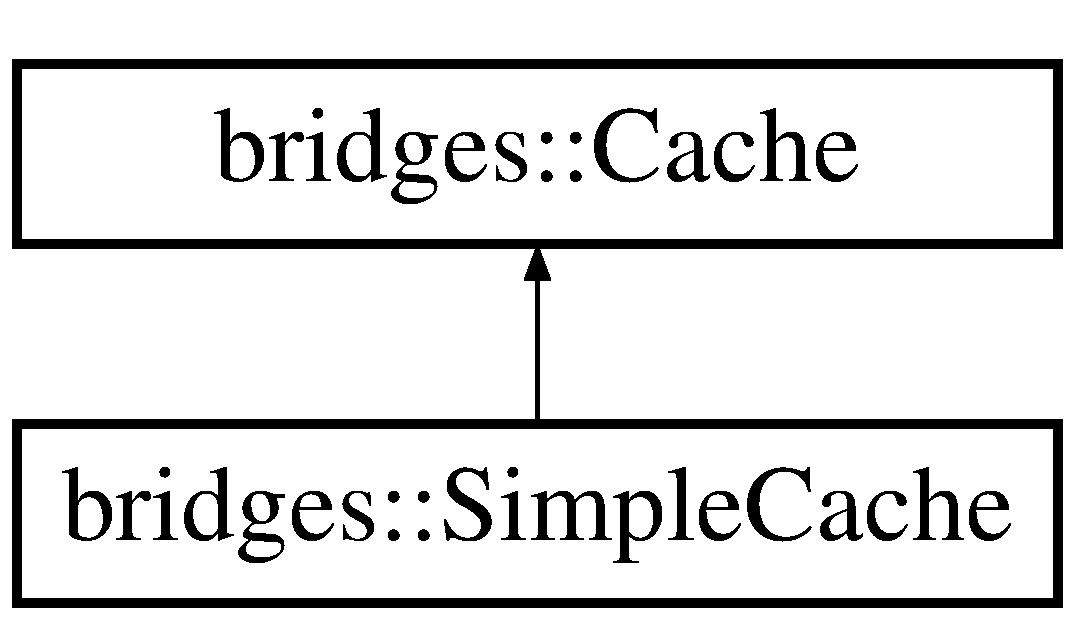
\includegraphics[height=2.000000cm]{classbridges_1_1_simple_cache}
\end{center}
\end{figure}
\subsection*{Public Member Functions}
\begin{DoxyCompactItemize}
\item 
\hyperlink{classbridges_1_1_simple_cache_af6454edafca975489988b8df61d1cd2a}{Simple\+Cache} ()
\item 
virtual bool \hyperlink{classbridges_1_1_simple_cache_a9af328045bad7c3bd4ed6cf99352bf07}{in\+Cache} (const std\+::string \&doc\+Name) noexcept(false) override
\item 
virtual std\+::string \hyperlink{classbridges_1_1_simple_cache_a905ad2e7fb1b6784a5f70caf024b157f}{get\+Doc} (const std\+::string \&doc\+Name) noexcept(false) override
\item 
virtual void \hyperlink{classbridges_1_1_simple_cache_a61264b1080a4458d6210c7cf6b4e8615}{put\+Doc} (const std\+::string \&doc\+Name, const std\+::string \&content) noexcept(false) override
\item 
bool \hyperlink{classbridges_1_1_simple_cache_a1a676acaaecd1e5368a3d51a654d93bc}{evict} (const std\+::string \&doc\+Name)
\begin{DoxyCompactList}\small\item\em evicts a document from the cache \end{DoxyCompactList}\end{DoxyCompactItemize}


\subsection{Constructor \& Destructor Documentation}
\mbox{\Hypertarget{classbridges_1_1_simple_cache_af6454edafca975489988b8df61d1cd2a}\label{classbridges_1_1_simple_cache_af6454edafca975489988b8df61d1cd2a}} 
\index{bridges\+::\+Simple\+Cache@{bridges\+::\+Simple\+Cache}!Simple\+Cache@{Simple\+Cache}}
\index{Simple\+Cache@{Simple\+Cache}!bridges\+::\+Simple\+Cache@{bridges\+::\+Simple\+Cache}}
\subsubsection{\texorpdfstring{Simple\+Cache()}{SimpleCache()}}
{\footnotesize\ttfamily bridges\+::\+Simple\+Cache\+::\+Simple\+Cache (\begin{DoxyParamCaption}{ }\end{DoxyParamCaption})\hspace{0.3cm}{\ttfamily [inline]}}



\subsection{Member Function Documentation}
\mbox{\Hypertarget{classbridges_1_1_simple_cache_a1a676acaaecd1e5368a3d51a654d93bc}\label{classbridges_1_1_simple_cache_a1a676acaaecd1e5368a3d51a654d93bc}} 
\index{bridges\+::\+Simple\+Cache@{bridges\+::\+Simple\+Cache}!evict@{evict}}
\index{evict@{evict}!bridges\+::\+Simple\+Cache@{bridges\+::\+Simple\+Cache}}
\subsubsection{\texorpdfstring{evict()}{evict()}}
{\footnotesize\ttfamily bool bridges\+::\+Simple\+Cache\+::evict (\begin{DoxyParamCaption}\item[{const std\+::string \&}]{doc\+Name }\end{DoxyParamCaption})\hspace{0.3cm}{\ttfamily [inline]}}



evicts a document from the cache 


\begin{DoxyParams}{Parameters}
{\em doc\+Name} & document to evict \\
\hline
\end{DoxyParams}
\begin{DoxyReturn}{Returns}
true on success 
\end{DoxyReturn}
\mbox{\Hypertarget{classbridges_1_1_simple_cache_a905ad2e7fb1b6784a5f70caf024b157f}\label{classbridges_1_1_simple_cache_a905ad2e7fb1b6784a5f70caf024b157f}} 
\index{bridges\+::\+Simple\+Cache@{bridges\+::\+Simple\+Cache}!get\+Doc@{get\+Doc}}
\index{get\+Doc@{get\+Doc}!bridges\+::\+Simple\+Cache@{bridges\+::\+Simple\+Cache}}
\subsubsection{\texorpdfstring{get\+Doc()}{getDoc()}}
{\footnotesize\ttfamily virtual std\+::string bridges\+::\+Simple\+Cache\+::get\+Doc (\begin{DoxyParamCaption}\item[{const std\+::string \&}]{doc\+Name }\end{DoxyParamCaption})\hspace{0.3cm}{\ttfamily [inline]}, {\ttfamily [override]}, {\ttfamily [virtual]}, {\ttfamily [noexcept]}}



Implements \hyperlink{classbridges_1_1_cache_abc1eaca36899e6e85df1c9a690f1d4dd}{bridges\+::\+Cache}.

\mbox{\Hypertarget{classbridges_1_1_simple_cache_a9af328045bad7c3bd4ed6cf99352bf07}\label{classbridges_1_1_simple_cache_a9af328045bad7c3bd4ed6cf99352bf07}} 
\index{bridges\+::\+Simple\+Cache@{bridges\+::\+Simple\+Cache}!in\+Cache@{in\+Cache}}
\index{in\+Cache@{in\+Cache}!bridges\+::\+Simple\+Cache@{bridges\+::\+Simple\+Cache}}
\subsubsection{\texorpdfstring{in\+Cache()}{inCache()}}
{\footnotesize\ttfamily virtual bool bridges\+::\+Simple\+Cache\+::in\+Cache (\begin{DoxyParamCaption}\item[{const std\+::string \&}]{doc\+Name }\end{DoxyParamCaption})\hspace{0.3cm}{\ttfamily [inline]}, {\ttfamily [override]}, {\ttfamily [virtual]}, {\ttfamily [noexcept]}}



Implements \hyperlink{classbridges_1_1_cache_abf3601225841d14dcd5611cd6a223ba4}{bridges\+::\+Cache}.

\mbox{\Hypertarget{classbridges_1_1_simple_cache_a61264b1080a4458d6210c7cf6b4e8615}\label{classbridges_1_1_simple_cache_a61264b1080a4458d6210c7cf6b4e8615}} 
\index{bridges\+::\+Simple\+Cache@{bridges\+::\+Simple\+Cache}!put\+Doc@{put\+Doc}}
\index{put\+Doc@{put\+Doc}!bridges\+::\+Simple\+Cache@{bridges\+::\+Simple\+Cache}}
\subsubsection{\texorpdfstring{put\+Doc()}{putDoc()}}
{\footnotesize\ttfamily virtual void bridges\+::\+Simple\+Cache\+::put\+Doc (\begin{DoxyParamCaption}\item[{const std\+::string \&}]{doc\+Name,  }\item[{const std\+::string \&}]{content }\end{DoxyParamCaption})\hspace{0.3cm}{\ttfamily [inline]}, {\ttfamily [override]}, {\ttfamily [virtual]}, {\ttfamily [noexcept]}}



Implements \hyperlink{classbridges_1_1_cache_ae74225542568a377fdcaf0354e466954}{bridges\+::\+Cache}.



The documentation for this class was generated from the following file\+:\begin{DoxyCompactItemize}
\item 
/home/erik/work/bridges/bridges-\/cxx/src/\hyperlink{_cache_8h}{Cache.\+h}\end{DoxyCompactItemize}

\hypertarget{classbridges_1_1datastructure_1_1_s_lelement}{}\section{bridges\+:\+:datastructure\+:\+:S\+Lelement$<$ E $>$ Class Template Reference}
\label{classbridges_1_1datastructure_1_1_s_lelement}\index{bridges\+::datastructure\+::\+S\+Lelement$<$ E $>$@{bridges\+::datastructure\+::\+S\+Lelement$<$ E $>$}}


{\ttfamily \#include $<$S\+Lelement.\+h$>$}

Inheritance diagram for bridges\+:\+:datastructure\+:\+:S\+Lelement$<$ E $>$\+:\begin{figure}[H]
\begin{center}
\leavevmode
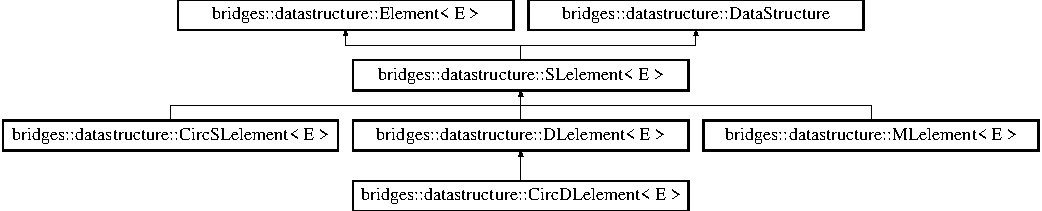
\includegraphics[height=2.839037cm]{classbridges_1_1datastructure_1_1_s_lelement}
\end{center}
\end{figure}


\subsection{Detailed Description}
\subsubsection*{template$<$typename E$>$\newline
class bridges\+::datastructure\+::\+S\+Lelement$<$ E $>$}

The singly linked list element, derived from \mbox{\hyperlink{classbridges_1_1datastructure_1_1_element}{Element}}. 

This class can be used to create singly linked elements, with a next \mbox{\hyperlink{classbridges_1_1datastructure_1_1_s_lelement}{S\+Lelement}} pointer

\begin{DoxySeeAlso}{See also}
There is a tutorial about Singly Linked Lists \+: \href{http://bridgesuncc.github.io/tutorials/SinglyLinkedList.html}{\tt http\+://bridgesuncc.\+github.\+io/tutorials/\+Singly\+Linked\+List.\+html}
\end{DoxySeeAlso}

\begin{DoxyParams}{Parameters}
{\em E} & the application data type\\
\hline
\end{DoxyParams}
\begin{DoxyAuthor}{Author}
Kalpathi Subramanian 
\end{DoxyAuthor}
\begin{DoxyDate}{Date}
6/11/15, 7/12/19 
\end{DoxyDate}
\subsection*{Classes}
\begin{DoxyCompactItemize}
\item 
class \mbox{\hyperlink{classbridges_1_1datastructure_1_1_s_lelement_1_1_s_lelement__constlisthelper}{S\+Lelement\+\_\+constlisthelper}}
\begin{DoxyCompactList}\small\item\em these are helper classes for \mbox{\hyperlink{classbridges_1_1datastructure_1_1_s_lelement}{S\+Lelement}} for easy iteration in a range for loop. It is not meant to be created by the bridges user. But it may be returned by \mbox{\hyperlink{classbridges_1_1_bridges}{Bridges}} to provide an S\+TL compliant list A\+PI. \end{DoxyCompactList}\item 
class \mbox{\hyperlink{classbridges_1_1datastructure_1_1_s_lelement_1_1_s_lelement__listhelper}{S\+Lelement\+\_\+listhelper}}
\begin{DoxyCompactList}\small\item\em these are helper classes for \mbox{\hyperlink{classbridges_1_1datastructure_1_1_s_lelement}{S\+Lelement}} for easy iteration in a range for loop. It is not meant to be created by the bridges user. But it may be returned by \mbox{\hyperlink{classbridges_1_1_bridges}{Bridges}} to provide an S\+TL compliant list A\+PI. \end{DoxyCompactList}\end{DoxyCompactItemize}
\subsection*{Public Member Functions}
\begin{DoxyCompactItemize}
\item 
\mbox{\hyperlink{classbridges_1_1datastructure_1_1_s_lelement_ac69e99f5b2b729a217160ee0517751aa}{S\+Lelement}} (\mbox{\hyperlink{classbridges_1_1datastructure_1_1_s_lelement}{S\+Lelement}} $\ast$\mbox{\hyperlink{classbridges_1_1datastructure_1_1_s_lelement_afc016a593a4a5aba82021ee34edadbfc}{next}}, const E \&val=E(), const string \&lab=string())
\item 
\mbox{\hyperlink{classbridges_1_1datastructure_1_1_s_lelement_a2f56e5f74a2cb43ab6ea718ae5bfdcbf}{S\+Lelement}} (const E \&val=E(), const string \&lab=string())
\item 
virtual const string \mbox{\hyperlink{classbridges_1_1datastructure_1_1_s_lelement_a602156aacacd73d1faa365d68d8af31b}{get\+D\+Stype}} () const override
\item 
virtual \mbox{\hyperlink{classbridges_1_1datastructure_1_1_s_lelement}{S\+Lelement}} $\ast$ \mbox{\hyperlink{classbridges_1_1datastructure_1_1_s_lelement_ae43dd771d9ced7cb17f1d35f34cd9a42}{get\+Next}} ()
\item 
virtual const \mbox{\hyperlink{classbridges_1_1datastructure_1_1_s_lelement}{S\+Lelement}} $\ast$ \mbox{\hyperlink{classbridges_1_1datastructure_1_1_s_lelement_a8c62cb82fa64bbfe9ebb7334a5fea417}{get\+Next}} () const
\item 
void \mbox{\hyperlink{classbridges_1_1datastructure_1_1_s_lelement_acf736223b4cd27b0771b262870d70b94}{set\+Next}} (\mbox{\hyperlink{classbridges_1_1datastructure_1_1_s_lelement}{S\+Lelement}} $\ast$n)
\end{DoxyCompactItemize}
\subsection*{Protected Member Functions}
\begin{DoxyCompactItemize}
\item 
virtual const pair$<$ string, string $>$ \mbox{\hyperlink{classbridges_1_1datastructure_1_1_s_lelement_a15d224314bbda510603042b504322410}{generate\+J\+S\+ON}} (vector$<$ const \mbox{\hyperlink{classbridges_1_1datastructure_1_1_s_lelement}{S\+Lelement}}$<$ E $>$ $\ast$$>$ nodes) const
\item 
virtual void \mbox{\hyperlink{classbridges_1_1datastructure_1_1_s_lelement_a81b68786cb93fe0f7edb48af789535a5}{get\+List\+Elements}} (vector$<$ const \mbox{\hyperlink{classbridges_1_1datastructure_1_1_s_lelement}{S\+Lelement}}$<$ E $>$ $\ast$$>$ \&nodes) const
\end{DoxyCompactItemize}
\subsection*{Protected Attributes}
\begin{DoxyCompactItemize}
\item 
\mbox{\hyperlink{classbridges_1_1datastructure_1_1_s_lelement}{S\+Lelement}} $\ast$ \mbox{\hyperlink{classbridges_1_1datastructure_1_1_s_lelement_afc016a593a4a5aba82021ee34edadbfc}{next}} = nullptr
\end{DoxyCompactItemize}
\subsection*{Additional Inherited Members}


\subsection{Constructor \& Destructor Documentation}
\mbox{\Hypertarget{classbridges_1_1datastructure_1_1_s_lelement_ac69e99f5b2b729a217160ee0517751aa}\label{classbridges_1_1datastructure_1_1_s_lelement_ac69e99f5b2b729a217160ee0517751aa}} 
\index{bridges\+::datastructure\+::\+S\+Lelement@{bridges\+::datastructure\+::\+S\+Lelement}!S\+Lelement@{S\+Lelement}}
\index{S\+Lelement@{S\+Lelement}!bridges\+::datastructure\+::\+S\+Lelement@{bridges\+::datastructure\+::\+S\+Lelement}}
\subsubsection{\texorpdfstring{S\+Lelement()}{SLelement()}\hspace{0.1cm}{\footnotesize\ttfamily [1/2]}}
{\footnotesize\ttfamily template$<$typename E$>$ \\
\mbox{\hyperlink{classbridges_1_1datastructure_1_1_s_lelement}{bridges\+::datastructure\+::\+S\+Lelement}}$<$ E $>$\+::\mbox{\hyperlink{classbridges_1_1datastructure_1_1_s_lelement}{S\+Lelement}} (\begin{DoxyParamCaption}\item[{\mbox{\hyperlink{classbridges_1_1datastructure_1_1_s_lelement}{S\+Lelement}}$<$ E $>$ $\ast$}]{next,  }\item[{const E \&}]{val = {\ttfamily E()},  }\item[{const string \&}]{lab = {\ttfamily string()} }\end{DoxyParamCaption})\hspace{0.3cm}{\ttfamily [inline]}}

Constructs an slelement with the provided value, label, and next slelement. The defaults will be used if not provided.


\begin{DoxyParams}{Parameters}
{\em val} & The data to hold \\
\hline
{\em lab} & The label to show \\
\hline
{\em next} & The next \mbox{\hyperlink{classbridges_1_1datastructure_1_1_s_lelement}{S\+Lelement}} \\
\hline
\end{DoxyParams}
\mbox{\Hypertarget{classbridges_1_1datastructure_1_1_s_lelement_a2f56e5f74a2cb43ab6ea718ae5bfdcbf}\label{classbridges_1_1datastructure_1_1_s_lelement_a2f56e5f74a2cb43ab6ea718ae5bfdcbf}} 
\index{bridges\+::datastructure\+::\+S\+Lelement@{bridges\+::datastructure\+::\+S\+Lelement}!S\+Lelement@{S\+Lelement}}
\index{S\+Lelement@{S\+Lelement}!bridges\+::datastructure\+::\+S\+Lelement@{bridges\+::datastructure\+::\+S\+Lelement}}
\subsubsection{\texorpdfstring{S\+Lelement()}{SLelement()}\hspace{0.1cm}{\footnotesize\ttfamily [2/2]}}
{\footnotesize\ttfamily template$<$typename E$>$ \\
\mbox{\hyperlink{classbridges_1_1datastructure_1_1_s_lelement}{bridges\+::datastructure\+::\+S\+Lelement}}$<$ E $>$\+::\mbox{\hyperlink{classbridges_1_1datastructure_1_1_s_lelement}{S\+Lelement}} (\begin{DoxyParamCaption}\item[{const E \&}]{val = {\ttfamily E()},  }\item[{const string \&}]{lab = {\ttfamily string()} }\end{DoxyParamCaption})\hspace{0.3cm}{\ttfamily [inline]}}

Constructs an slelement with the provided value and label, setting the next slelement to N\+U\+LL. The defaults will be used if not provided.


\begin{DoxyParams}{Parameters}
{\em val} & The data to hold \\
\hline
{\em lab} & The label to show \\
\hline
\end{DoxyParams}


\subsection{Member Function Documentation}
\mbox{\Hypertarget{classbridges_1_1datastructure_1_1_s_lelement_a15d224314bbda510603042b504322410}\label{classbridges_1_1datastructure_1_1_s_lelement_a15d224314bbda510603042b504322410}} 
\index{bridges\+::datastructure\+::\+S\+Lelement@{bridges\+::datastructure\+::\+S\+Lelement}!generate\+J\+S\+ON@{generate\+J\+S\+ON}}
\index{generate\+J\+S\+ON@{generate\+J\+S\+ON}!bridges\+::datastructure\+::\+S\+Lelement@{bridges\+::datastructure\+::\+S\+Lelement}}
\subsubsection{\texorpdfstring{generate\+J\+S\+O\+N()}{generateJSON()}}
{\footnotesize\ttfamily template$<$typename E$>$ \\
virtual const pair$<$string, string$>$ \mbox{\hyperlink{classbridges_1_1datastructure_1_1_s_lelement}{bridges\+::datastructure\+::\+S\+Lelement}}$<$ E $>$\+::generate\+J\+S\+ON (\begin{DoxyParamCaption}\item[{vector$<$ const \mbox{\hyperlink{classbridges_1_1datastructure_1_1_s_lelement}{S\+Lelement}}$<$ E $>$ $\ast$$>$}]{nodes }\end{DoxyParamCaption}) const\hspace{0.3cm}{\ttfamily [inline]}, {\ttfamily [protected]}, {\ttfamily [virtual]}}

Generates the J\+S\+ON representation of the nodes and links \begin{DoxyReturn}{Returns}
J\+S\+ON string pair containing the nodes and links 
\end{DoxyReturn}
\mbox{\Hypertarget{classbridges_1_1datastructure_1_1_s_lelement_a602156aacacd73d1faa365d68d8af31b}\label{classbridges_1_1datastructure_1_1_s_lelement_a602156aacacd73d1faa365d68d8af31b}} 
\index{bridges\+::datastructure\+::\+S\+Lelement@{bridges\+::datastructure\+::\+S\+Lelement}!get\+D\+Stype@{get\+D\+Stype}}
\index{get\+D\+Stype@{get\+D\+Stype}!bridges\+::datastructure\+::\+S\+Lelement@{bridges\+::datastructure\+::\+S\+Lelement}}
\subsubsection{\texorpdfstring{get\+D\+Stype()}{getDStype()}}
{\footnotesize\ttfamily template$<$typename E$>$ \\
virtual const string \mbox{\hyperlink{classbridges_1_1datastructure_1_1_s_lelement}{bridges\+::datastructure\+::\+S\+Lelement}}$<$ E $>$\+::get\+D\+Stype (\begin{DoxyParamCaption}{ }\end{DoxyParamCaption}) const\hspace{0.3cm}{\ttfamily [inline]}, {\ttfamily [override]}, {\ttfamily [virtual]}}

Returns the data structure name

\begin{DoxyReturn}{Returns}
The string representation of this data structure type 
\end{DoxyReturn}


Implements \mbox{\hyperlink{classbridges_1_1datastructure_1_1_data_structure_a4ff66cb34409f11fe9fc647f6d8a22ce}{bridges\+::datastructure\+::\+Data\+Structure}}.



Reimplemented in \mbox{\hyperlink{classbridges_1_1datastructure_1_1_m_lelement_a735c3cb43648b4d4e7d3316cdc1a1952}{bridges\+::datastructure\+::\+M\+Lelement$<$ E $>$}}, \mbox{\hyperlink{classbridges_1_1datastructure_1_1_circ_d_lelement_aec7f9b9dc6626c1a872feb91cd65425d}{bridges\+::datastructure\+::\+Circ\+D\+Lelement$<$ E $>$}}, \mbox{\hyperlink{classbridges_1_1datastructure_1_1_circ_s_lelement_a775ba08a7811fe91c396cb27ba9343ab}{bridges\+::datastructure\+::\+Circ\+S\+Lelement$<$ E $>$}}, and \mbox{\hyperlink{classbridges_1_1datastructure_1_1_d_lelement_a736ba8e6901608fb0ab04d781d2cceee}{bridges\+::datastructure\+::\+D\+Lelement$<$ E $>$}}.

\mbox{\Hypertarget{classbridges_1_1datastructure_1_1_s_lelement_a81b68786cb93fe0f7edb48af789535a5}\label{classbridges_1_1datastructure_1_1_s_lelement_a81b68786cb93fe0f7edb48af789535a5}} 
\index{bridges\+::datastructure\+::\+S\+Lelement@{bridges\+::datastructure\+::\+S\+Lelement}!get\+List\+Elements@{get\+List\+Elements}}
\index{get\+List\+Elements@{get\+List\+Elements}!bridges\+::datastructure\+::\+S\+Lelement@{bridges\+::datastructure\+::\+S\+Lelement}}
\subsubsection{\texorpdfstring{get\+List\+Elements()}{getListElements()}}
{\footnotesize\ttfamily template$<$typename E$>$ \\
virtual void \mbox{\hyperlink{classbridges_1_1datastructure_1_1_s_lelement}{bridges\+::datastructure\+::\+S\+Lelement}}$<$ E $>$\+::get\+List\+Elements (\begin{DoxyParamCaption}\item[{vector$<$ const \mbox{\hyperlink{classbridges_1_1datastructure_1_1_s_lelement}{S\+Lelement}}$<$ E $>$ $\ast$$>$ \&}]{nodes }\end{DoxyParamCaption}) const\hspace{0.3cm}{\ttfamily [inline]}, {\ttfamily [protected]}, {\ttfamily [virtual]}}

Get the list of nodes


\begin{DoxyParams}{Parameters}
{\em nodes} & The list of nodes \\
\hline
\end{DoxyParams}
\mbox{\Hypertarget{classbridges_1_1datastructure_1_1_s_lelement_ae43dd771d9ced7cb17f1d35f34cd9a42}\label{classbridges_1_1datastructure_1_1_s_lelement_ae43dd771d9ced7cb17f1d35f34cd9a42}} 
\index{bridges\+::datastructure\+::\+S\+Lelement@{bridges\+::datastructure\+::\+S\+Lelement}!get\+Next@{get\+Next}}
\index{get\+Next@{get\+Next}!bridges\+::datastructure\+::\+S\+Lelement@{bridges\+::datastructure\+::\+S\+Lelement}}
\subsubsection{\texorpdfstring{get\+Next()}{getNext()}\hspace{0.1cm}{\footnotesize\ttfamily [1/2]}}
{\footnotesize\ttfamily template$<$typename E$>$ \\
virtual \mbox{\hyperlink{classbridges_1_1datastructure_1_1_s_lelement}{S\+Lelement}}$\ast$ \mbox{\hyperlink{classbridges_1_1datastructure_1_1_s_lelement}{bridges\+::datastructure\+::\+S\+Lelement}}$<$ E $>$\+::get\+Next (\begin{DoxyParamCaption}{ }\end{DoxyParamCaption})\hspace{0.3cm}{\ttfamily [inline]}, {\ttfamily [virtual]}}

Returns the next element in the list \begin{DoxyReturn}{Returns}
The next \mbox{\hyperlink{classbridges_1_1datastructure_1_1_s_lelement}{S\+Lelement}} 
\end{DoxyReturn}


Reimplemented in \mbox{\hyperlink{classbridges_1_1datastructure_1_1_m_lelement_a47b417db0b948b6899eece572bef9274}{bridges\+::datastructure\+::\+M\+Lelement$<$ E $>$}}, \mbox{\hyperlink{classbridges_1_1datastructure_1_1_circ_d_lelement_a80681d0382643a6df21da1bec4067004}{bridges\+::datastructure\+::\+Circ\+D\+Lelement$<$ E $>$}}, \mbox{\hyperlink{classbridges_1_1datastructure_1_1_circ_s_lelement_aff77056ace1361a35a09dc006eba34a3}{bridges\+::datastructure\+::\+Circ\+S\+Lelement$<$ E $>$}}, and \mbox{\hyperlink{classbridges_1_1datastructure_1_1_d_lelement_a63212051ea77d74bd751dea00288d2be}{bridges\+::datastructure\+::\+D\+Lelement$<$ E $>$}}.

\mbox{\Hypertarget{classbridges_1_1datastructure_1_1_s_lelement_a8c62cb82fa64bbfe9ebb7334a5fea417}\label{classbridges_1_1datastructure_1_1_s_lelement_a8c62cb82fa64bbfe9ebb7334a5fea417}} 
\index{bridges\+::datastructure\+::\+S\+Lelement@{bridges\+::datastructure\+::\+S\+Lelement}!get\+Next@{get\+Next}}
\index{get\+Next@{get\+Next}!bridges\+::datastructure\+::\+S\+Lelement@{bridges\+::datastructure\+::\+S\+Lelement}}
\subsubsection{\texorpdfstring{get\+Next()}{getNext()}\hspace{0.1cm}{\footnotesize\ttfamily [2/2]}}
{\footnotesize\ttfamily template$<$typename E$>$ \\
virtual const \mbox{\hyperlink{classbridges_1_1datastructure_1_1_s_lelement}{S\+Lelement}}$\ast$ \mbox{\hyperlink{classbridges_1_1datastructure_1_1_s_lelement}{bridges\+::datastructure\+::\+S\+Lelement}}$<$ E $>$\+::get\+Next (\begin{DoxyParamCaption}{ }\end{DoxyParamCaption}) const\hspace{0.3cm}{\ttfamily [inline]}, {\ttfamily [virtual]}}

Returns the next element in the list -\/ Constant version \begin{DoxyReturn}{Returns}
The next \mbox{\hyperlink{classbridges_1_1datastructure_1_1_s_lelement}{S\+Lelement}} 
\end{DoxyReturn}


Reimplemented in \mbox{\hyperlink{classbridges_1_1datastructure_1_1_m_lelement_a611b3e7d54fdfbc622004a50ca718e6e}{bridges\+::datastructure\+::\+M\+Lelement$<$ E $>$}}, \mbox{\hyperlink{classbridges_1_1datastructure_1_1_circ_d_lelement_a3b54f07ffa49151ed13d8b8df964a4ee}{bridges\+::datastructure\+::\+Circ\+D\+Lelement$<$ E $>$}}, and \mbox{\hyperlink{classbridges_1_1datastructure_1_1_d_lelement_a8599e5be5fc1771d4e8a40f6de67b4a7}{bridges\+::datastructure\+::\+D\+Lelement$<$ E $>$}}.

\mbox{\Hypertarget{classbridges_1_1datastructure_1_1_s_lelement_acf736223b4cd27b0771b262870d70b94}\label{classbridges_1_1datastructure_1_1_s_lelement_acf736223b4cd27b0771b262870d70b94}} 
\index{bridges\+::datastructure\+::\+S\+Lelement@{bridges\+::datastructure\+::\+S\+Lelement}!set\+Next@{set\+Next}}
\index{set\+Next@{set\+Next}!bridges\+::datastructure\+::\+S\+Lelement@{bridges\+::datastructure\+::\+S\+Lelement}}
\subsubsection{\texorpdfstring{set\+Next()}{setNext()}}
{\footnotesize\ttfamily template$<$typename E$>$ \\
void \mbox{\hyperlink{classbridges_1_1datastructure_1_1_s_lelement}{bridges\+::datastructure\+::\+S\+Lelement}}$<$ E $>$\+::set\+Next (\begin{DoxyParamCaption}\item[{\mbox{\hyperlink{classbridges_1_1datastructure_1_1_s_lelement}{S\+Lelement}}$<$ E $>$ $\ast$}]{n }\end{DoxyParamCaption})\hspace{0.3cm}{\ttfamily [inline]}}

Sets next link to \char`\"{}n\char`\"{}


\begin{DoxyParams}{Parameters}
{\em n} & The next \mbox{\hyperlink{classbridges_1_1datastructure_1_1_s_lelement}{S\+Lelement}} \\
\hline
\end{DoxyParams}


\subsection{Member Data Documentation}
\mbox{\Hypertarget{classbridges_1_1datastructure_1_1_s_lelement_afc016a593a4a5aba82021ee34edadbfc}\label{classbridges_1_1datastructure_1_1_s_lelement_afc016a593a4a5aba82021ee34edadbfc}} 
\index{bridges\+::datastructure\+::\+S\+Lelement@{bridges\+::datastructure\+::\+S\+Lelement}!next@{next}}
\index{next@{next}!bridges\+::datastructure\+::\+S\+Lelement@{bridges\+::datastructure\+::\+S\+Lelement}}
\subsubsection{\texorpdfstring{next}{next}}
{\footnotesize\ttfamily template$<$typename E$>$ \\
\mbox{\hyperlink{classbridges_1_1datastructure_1_1_s_lelement}{S\+Lelement}}$\ast$ \mbox{\hyperlink{classbridges_1_1datastructure_1_1_s_lelement}{bridges\+::datastructure\+::\+S\+Lelement}}$<$ E $>$\+::next = nullptr\hspace{0.3cm}{\ttfamily [protected]}}



The documentation for this class was generated from the following file\+:\begin{DoxyCompactItemize}
\item 
/\+Users/kalpathi/gr/bridges/client/cxx/src/\mbox{\hyperlink{_s_lelement_8h}{S\+Lelement.\+h}}\end{DoxyCompactItemize}

\hypertarget{classbridges_1_1datastructure_1_1_s_lelement_1_1_s_lelement__constlisthelper}{}\section{bridges\+:\+:datastructure\+:\+:S\+Lelement$<$ E $>$\+:\+:S\+Lelement\+\_\+constlisthelper Class Reference}
\label{classbridges_1_1datastructure_1_1_s_lelement_1_1_s_lelement__constlisthelper}\index{bridges\+::datastructure\+::\+S\+Lelement$<$ E $>$\+::\+S\+Lelement\+\_\+constlisthelper@{bridges\+::datastructure\+::\+S\+Lelement$<$ E $>$\+::\+S\+Lelement\+\_\+constlisthelper}}


{\ttfamily \#include $<$S\+Lelement.\+h$>$}



\subsection{Detailed Description}
\subsubsection*{template$<$typename E$>$\newline
class bridges\+::datastructure\+::\+S\+Lelement$<$ E $>$\+::\+S\+Lelement\+\_\+constlisthelper}

these are helper classes for \hyperlink{classbridges_1_1datastructure_1_1_s_lelement}{S\+Lelement} for easy iteration in a range for loop. It is not meant to be created by the bridges user. But it may be returned by \hyperlink{classbridges_1_1_bridges}{Bridges} to provide an S\+TL compliant list A\+PI. \subsection*{Classes}
\begin{DoxyCompactItemize}
\item 
class \hyperlink{classbridges_1_1datastructure_1_1_s_lelement_1_1_s_lelement__constlisthelper_1_1iterator}{iterator}
\end{DoxyCompactItemize}
\subsection*{Public Member Functions}
\begin{DoxyCompactItemize}
\item 
\hyperlink{classbridges_1_1datastructure_1_1_s_lelement_1_1_s_lelement__constlisthelper_aab5d445c4ff680098daa796b76345cfc}{S\+Lelement\+\_\+constlisthelper} (typename \hyperlink{classbridges_1_1datastructure_1_1_s_lelement}{bridges\+::datastructure\+::\+S\+Lelement}$<$ E $>$ const $\ast$s)
\item 
\hyperlink{classbridges_1_1datastructure_1_1_s_lelement_1_1_s_lelement__constlisthelper_1_1iterator}{iterator} \hyperlink{classbridges_1_1datastructure_1_1_s_lelement_1_1_s_lelement__constlisthelper_a2e2adc3b30f68514a90af399f47624ac}{begin} ()
\item 
\hyperlink{classbridges_1_1datastructure_1_1_s_lelement_1_1_s_lelement__constlisthelper_1_1iterator}{iterator} \hyperlink{classbridges_1_1datastructure_1_1_s_lelement_1_1_s_lelement__constlisthelper_a4ec5e5fe4b53638dfada78d44c7dd5b2}{end} ()
\end{DoxyCompactItemize}


\subsection{Constructor \& Destructor Documentation}
\mbox{\Hypertarget{classbridges_1_1datastructure_1_1_s_lelement_1_1_s_lelement__constlisthelper_aab5d445c4ff680098daa796b76345cfc}\label{classbridges_1_1datastructure_1_1_s_lelement_1_1_s_lelement__constlisthelper_aab5d445c4ff680098daa796b76345cfc}} 
\index{bridges\+::datastructure\+::\+S\+Lelement\+::\+S\+Lelement\+\_\+constlisthelper@{bridges\+::datastructure\+::\+S\+Lelement\+::\+S\+Lelement\+\_\+constlisthelper}!S\+Lelement\+\_\+constlisthelper@{S\+Lelement\+\_\+constlisthelper}}
\index{S\+Lelement\+\_\+constlisthelper@{S\+Lelement\+\_\+constlisthelper}!bridges\+::datastructure\+::\+S\+Lelement\+::\+S\+Lelement\+\_\+constlisthelper@{bridges\+::datastructure\+::\+S\+Lelement\+::\+S\+Lelement\+\_\+constlisthelper}}
\subsubsection{\texorpdfstring{S\+Lelement\+\_\+constlisthelper()}{SLelement\_constlisthelper()}}
{\footnotesize\ttfamily template$<$typename E$>$ \\
\hyperlink{classbridges_1_1datastructure_1_1_s_lelement}{bridges\+::datastructure\+::\+S\+Lelement}$<$ E $>$\+::S\+Lelement\+\_\+constlisthelper\+::\+S\+Lelement\+\_\+constlisthelper (\begin{DoxyParamCaption}\item[{typename \hyperlink{classbridges_1_1datastructure_1_1_s_lelement}{bridges\+::datastructure\+::\+S\+Lelement}$<$ E $>$ const $\ast$}]{s }\end{DoxyParamCaption})\hspace{0.3cm}{\ttfamily [inline]}}



\subsection{Member Function Documentation}
\mbox{\Hypertarget{classbridges_1_1datastructure_1_1_s_lelement_1_1_s_lelement__constlisthelper_a2e2adc3b30f68514a90af399f47624ac}\label{classbridges_1_1datastructure_1_1_s_lelement_1_1_s_lelement__constlisthelper_a2e2adc3b30f68514a90af399f47624ac}} 
\index{bridges\+::datastructure\+::\+S\+Lelement\+::\+S\+Lelement\+\_\+constlisthelper@{bridges\+::datastructure\+::\+S\+Lelement\+::\+S\+Lelement\+\_\+constlisthelper}!begin@{begin}}
\index{begin@{begin}!bridges\+::datastructure\+::\+S\+Lelement\+::\+S\+Lelement\+\_\+constlisthelper@{bridges\+::datastructure\+::\+S\+Lelement\+::\+S\+Lelement\+\_\+constlisthelper}}
\subsubsection{\texorpdfstring{begin()}{begin()}}
{\footnotesize\ttfamily template$<$typename E$>$ \\
\hyperlink{classbridges_1_1datastructure_1_1_s_lelement_1_1_s_lelement__constlisthelper_1_1iterator}{iterator} \hyperlink{classbridges_1_1datastructure_1_1_s_lelement}{bridges\+::datastructure\+::\+S\+Lelement}$<$ E $>$\+::S\+Lelement\+\_\+constlisthelper\+::begin (\begin{DoxyParamCaption}{ }\end{DoxyParamCaption})\hspace{0.3cm}{\ttfamily [inline]}}

\mbox{\Hypertarget{classbridges_1_1datastructure_1_1_s_lelement_1_1_s_lelement__constlisthelper_a4ec5e5fe4b53638dfada78d44c7dd5b2}\label{classbridges_1_1datastructure_1_1_s_lelement_1_1_s_lelement__constlisthelper_a4ec5e5fe4b53638dfada78d44c7dd5b2}} 
\index{bridges\+::datastructure\+::\+S\+Lelement\+::\+S\+Lelement\+\_\+constlisthelper@{bridges\+::datastructure\+::\+S\+Lelement\+::\+S\+Lelement\+\_\+constlisthelper}!end@{end}}
\index{end@{end}!bridges\+::datastructure\+::\+S\+Lelement\+::\+S\+Lelement\+\_\+constlisthelper@{bridges\+::datastructure\+::\+S\+Lelement\+::\+S\+Lelement\+\_\+constlisthelper}}
\subsubsection{\texorpdfstring{end()}{end()}}
{\footnotesize\ttfamily template$<$typename E$>$ \\
\hyperlink{classbridges_1_1datastructure_1_1_s_lelement_1_1_s_lelement__constlisthelper_1_1iterator}{iterator} \hyperlink{classbridges_1_1datastructure_1_1_s_lelement}{bridges\+::datastructure\+::\+S\+Lelement}$<$ E $>$\+::S\+Lelement\+\_\+constlisthelper\+::end (\begin{DoxyParamCaption}{ }\end{DoxyParamCaption})\hspace{0.3cm}{\ttfamily [inline]}}



The documentation for this class was generated from the following file\+:\begin{DoxyCompactItemize}
\item 
/home/erik/work/bridges/bridges-\/cxx/src/\hyperlink{_s_lelement_8h}{S\+Lelement.\+h}\end{DoxyCompactItemize}

\hypertarget{classbridges_1_1datastructure_1_1_s_lelement_1_1_s_lelement__listhelper}{}\section{bridges\+::datastructure\+::S\+Lelement$<$ E $>$\+::S\+Lelement\+\_\+listhelper Class Reference}
\label{classbridges_1_1datastructure_1_1_s_lelement_1_1_s_lelement__listhelper}\index{bridges::datastructure::SLelement$<$ E $>$::SLelement\_listhelper@{bridges::datastructure::SLelement$<$ E $>$::SLelement\_listhelper}}


{\ttfamily \#include $<$S\+Lelement.\+h$>$}



\subsection{Detailed Description}
\subsubsection*{template$<$typename E$>$\newline
class bridges\+::datastructure\+::\+S\+Lelement$<$ E $>$\+::\+S\+Lelement\+\_\+listhelper}

these are helper classes for \mbox{\hyperlink{classbridges_1_1datastructure_1_1_s_lelement}{S\+Lelement}} for easy iteration in a range for loop. It is not meant to be created by the bridges user. But it may be returned by \mbox{\hyperlink{classbridges_1_1_bridges}{Bridges}} to provide an S\+TL compliant list A\+PI. \subsection*{Classes}
\begin{DoxyCompactItemize}
\item 
class \mbox{\hyperlink{classbridges_1_1datastructure_1_1_s_lelement_1_1_s_lelement__listhelper_1_1iterator}{iterator}}
\end{DoxyCompactItemize}
\subsection*{Public Member Functions}
\begin{DoxyCompactItemize}
\item 
\mbox{\hyperlink{classbridges_1_1datastructure_1_1_s_lelement_1_1_s_lelement__listhelper_af58b3e4590449c12ca505a8f05740046}{S\+Lelement\+\_\+listhelper}} (typename \mbox{\hyperlink{classbridges_1_1datastructure_1_1_s_lelement}{bridges\+::datastructure\+::\+S\+Lelement}}$<$ E $>$ $\ast$s)
\item 
\mbox{\hyperlink{classbridges_1_1datastructure_1_1_s_lelement_1_1_s_lelement__listhelper_1_1iterator}{iterator}} \mbox{\hyperlink{classbridges_1_1datastructure_1_1_s_lelement_1_1_s_lelement__listhelper_a9bc74da8d0ae6cfc9506ea9480c33a15}{begin}} ()
\item 
\mbox{\hyperlink{classbridges_1_1datastructure_1_1_s_lelement_1_1_s_lelement__listhelper_1_1iterator}{iterator}} \mbox{\hyperlink{classbridges_1_1datastructure_1_1_s_lelement_1_1_s_lelement__listhelper_aecbbc35682d82fa86a746b9a588525d0}{end}} ()
\end{DoxyCompactItemize}


\subsection{Constructor \& Destructor Documentation}
\mbox{\Hypertarget{classbridges_1_1datastructure_1_1_s_lelement_1_1_s_lelement__listhelper_af58b3e4590449c12ca505a8f05740046}\label{classbridges_1_1datastructure_1_1_s_lelement_1_1_s_lelement__listhelper_af58b3e4590449c12ca505a8f05740046}} 
\index{bridges::datastructure::SLelement$<$ E $>$::SLelement\_listhelper@{bridges::datastructure::SLelement$<$ E $>$::SLelement\_listhelper}!SLelement\_listhelper@{SLelement\_listhelper}}
\index{SLelement\_listhelper@{SLelement\_listhelper}!bridges::datastructure::SLelement$<$ E $>$::SLelement\_listhelper@{bridges::datastructure::SLelement$<$ E $>$::SLelement\_listhelper}}
\subsubsection{\texorpdfstring{SLelement\_listhelper()}{SLelement\_listhelper()}}
{\footnotesize\ttfamily template$<$typename E$>$ \\
\mbox{\hyperlink{classbridges_1_1datastructure_1_1_s_lelement}{bridges\+::datastructure\+::\+S\+Lelement}}$<$ E $>$\+::S\+Lelement\+\_\+listhelper\+::\+S\+Lelement\+\_\+listhelper (\begin{DoxyParamCaption}\item[{typename \mbox{\hyperlink{classbridges_1_1datastructure_1_1_s_lelement}{bridges\+::datastructure\+::\+S\+Lelement}}$<$ E $>$ $\ast$}]{s }\end{DoxyParamCaption})\hspace{0.3cm}{\ttfamily [inline]}}



\subsection{Member Function Documentation}
\mbox{\Hypertarget{classbridges_1_1datastructure_1_1_s_lelement_1_1_s_lelement__listhelper_a9bc74da8d0ae6cfc9506ea9480c33a15}\label{classbridges_1_1datastructure_1_1_s_lelement_1_1_s_lelement__listhelper_a9bc74da8d0ae6cfc9506ea9480c33a15}} 
\index{bridges::datastructure::SLelement$<$ E $>$::SLelement\_listhelper@{bridges::datastructure::SLelement$<$ E $>$::SLelement\_listhelper}!begin@{begin}}
\index{begin@{begin}!bridges::datastructure::SLelement$<$ E $>$::SLelement\_listhelper@{bridges::datastructure::SLelement$<$ E $>$::SLelement\_listhelper}}
\subsubsection{\texorpdfstring{begin()}{begin()}}
{\footnotesize\ttfamily template$<$typename E$>$ \\
\mbox{\hyperlink{classbridges_1_1datastructure_1_1_s_lelement_1_1_s_lelement__listhelper_1_1iterator}{iterator}} \mbox{\hyperlink{classbridges_1_1datastructure_1_1_s_lelement}{bridges\+::datastructure\+::\+S\+Lelement}}$<$ E $>$\+::S\+Lelement\+\_\+listhelper\+::begin (\begin{DoxyParamCaption}{ }\end{DoxyParamCaption})\hspace{0.3cm}{\ttfamily [inline]}}

\mbox{\Hypertarget{classbridges_1_1datastructure_1_1_s_lelement_1_1_s_lelement__listhelper_aecbbc35682d82fa86a746b9a588525d0}\label{classbridges_1_1datastructure_1_1_s_lelement_1_1_s_lelement__listhelper_aecbbc35682d82fa86a746b9a588525d0}} 
\index{bridges::datastructure::SLelement$<$ E $>$::SLelement\_listhelper@{bridges::datastructure::SLelement$<$ E $>$::SLelement\_listhelper}!end@{end}}
\index{end@{end}!bridges::datastructure::SLelement$<$ E $>$::SLelement\_listhelper@{bridges::datastructure::SLelement$<$ E $>$::SLelement\_listhelper}}
\subsubsection{\texorpdfstring{end()}{end()}}
{\footnotesize\ttfamily template$<$typename E$>$ \\
\mbox{\hyperlink{classbridges_1_1datastructure_1_1_s_lelement_1_1_s_lelement__listhelper_1_1iterator}{iterator}} \mbox{\hyperlink{classbridges_1_1datastructure_1_1_s_lelement}{bridges\+::datastructure\+::\+S\+Lelement}}$<$ E $>$\+::S\+Lelement\+\_\+listhelper\+::end (\begin{DoxyParamCaption}{ }\end{DoxyParamCaption})\hspace{0.3cm}{\ttfamily [inline]}}



The documentation for this class was generated from the following file\+:\begin{DoxyCompactItemize}
\item 
/\+Users/kalpathi/gr/bridges/cxx/src/\mbox{\hyperlink{_s_lelement_8h}{S\+Lelement.\+h}}\end{DoxyCompactItemize}

\hypertarget{classsio_1_1socket}{}\doxysection{sio\+::socket Class Reference}
\label{classsio_1_1socket}\index{sio::socket@{sio::socket}}


{\ttfamily \#include $<$sio\+\_\+socket.\+h$>$}

\doxysubsection*{Public Types}
\begin{DoxyCompactItemize}
\item 
typedef std\+::function$<$ void(const std\+::string \&name, \mbox{\hyperlink{classsio_1_1message_a6340b6fef57e4516eb17928b1885a615}{message\+::ptr}} const  \&\mbox{\hyperlink{classsio_1_1message}{message}}, bool need\+\_\+ack, \mbox{\hyperlink{classsio_1_1message_1_1list}{message\+::list}} \&ack\+\_\+message)$>$ \mbox{\hyperlink{classsio_1_1socket_a426d9236f95762375d3b86caa2b4faaf}{event\+\_\+listener\+\_\+aux}}
\item 
typedef std\+::function$<$ void(\mbox{\hyperlink{classsio_1_1event}{event}} \&\mbox{\hyperlink{classsio_1_1event}{event}})$>$ \mbox{\hyperlink{classsio_1_1socket_ae0b1d93ef97af0d6d4f588e1e2a103b5}{event\+\_\+listener}}
\item 
typedef std\+::function$<$ void(\mbox{\hyperlink{classsio_1_1message_a6340b6fef57e4516eb17928b1885a615}{message\+::ptr}} const  \&\mbox{\hyperlink{classsio_1_1message}{message}})$>$ \mbox{\hyperlink{classsio_1_1socket_aecfea28271032e09dde1567bbfa97898}{error\+\_\+listener}}
\item 
typedef std\+::shared\+\_\+ptr$<$ \mbox{\hyperlink{classsio_1_1socket}{socket}} $>$ \mbox{\hyperlink{classsio_1_1socket_afb4f5829acfc5c8181ddb7174c501593}{ptr}}
\end{DoxyCompactItemize}
\doxysubsection*{Public Member Functions}
\begin{DoxyCompactItemize}
\item 
\mbox{\hyperlink{classsio_1_1socket_a801ded60fce567ad253a3c2740b79ddf}{$\sim$socket}} ()
\item 
void \mbox{\hyperlink{classsio_1_1socket_ab7b366ed08cef9820db1bd019a8c06ec}{on}} (std\+::string const \&event\+\_\+name, \mbox{\hyperlink{classsio_1_1socket_ae0b1d93ef97af0d6d4f588e1e2a103b5}{event\+\_\+listener}} const \&func)
\item 
void \mbox{\hyperlink{classsio_1_1socket_a6d3adaddc50f1a407e58d74b6d3d1367}{on}} (std\+::string const \&event\+\_\+name, \mbox{\hyperlink{classsio_1_1socket_a426d9236f95762375d3b86caa2b4faaf}{event\+\_\+listener\+\_\+aux}} const \&func)
\item 
void \mbox{\hyperlink{classsio_1_1socket_a7be26cf14d0611636c486a11a2b2ac02}{off}} (std\+::string const \&event\+\_\+name)
\item 
void \mbox{\hyperlink{classsio_1_1socket_a34e500f6baec2a9619887aa97cd7b794}{off\+\_\+all}} ()
\item 
void \mbox{\hyperlink{classsio_1_1socket_ae5073be58def64d16ead9806c24df8ec}{close}} ()
\item 
void \mbox{\hyperlink{classsio_1_1socket_a2296dfef16e09b35201866d2cba15a14}{on\+\_\+error}} (\mbox{\hyperlink{classsio_1_1socket_aecfea28271032e09dde1567bbfa97898}{error\+\_\+listener}} const \&l)
\item 
void \mbox{\hyperlink{classsio_1_1socket_a5528f1721aafc0cdd20effb9a80db087}{off\+\_\+error}} ()
\item 
void \mbox{\hyperlink{classsio_1_1socket_a76a3f52dec0e3fc16721183faa0e3def}{emit}} (std\+::string const \&name, \mbox{\hyperlink{classsio_1_1message_1_1list}{message\+::list}} const \&msglist=nullptr, std\+::function$<$ void(\mbox{\hyperlink{classsio_1_1message_1_1list}{message\+::list}} const \&)$>$ const \&ack=nullptr)
\item 
std\+::string const  \& \mbox{\hyperlink{classsio_1_1socket_ae0c48ebc168d677baaaefe45217f1185}{get\+\_\+namespace}} () const
\end{DoxyCompactItemize}
\doxysubsection*{Protected Member Functions}
\begin{DoxyCompactItemize}
\item 
\mbox{\hyperlink{classsio_1_1socket_ab4abbc8aa5356f4f48f0b1fa66c08e4b}{socket}} (\mbox{\hyperlink{classsio_1_1socket_a9598885c403f201c146fd19d243051df}{client\+\_\+impl}} $\ast$, std\+::string const \&)
\item 
void \mbox{\hyperlink{classsio_1_1socket_a1c4687fdfc7d6fbbfa98b56ba5aa4030}{on\+\_\+connected}} ()
\item 
void \mbox{\hyperlink{classsio_1_1socket_abf80872f56ac056f3379daf23b31ed23}{on\+\_\+close}} ()
\item 
void \mbox{\hyperlink{classsio_1_1socket_a8a793585b4aeb090bc001036d6786f97}{on\+\_\+open}} ()
\item 
void \mbox{\hyperlink{classsio_1_1socket_a20197f82bb7464e9c530ce27e9f0a01a}{on\+\_\+disconnect}} ()
\item 
void \mbox{\hyperlink{classsio_1_1socket_ac91742e3084791e30551e72e7ba17609}{on\+\_\+message\+\_\+packet}} (packet const \&p)
\end{DoxyCompactItemize}
\doxysubsection*{Friends}
\begin{DoxyCompactItemize}
\item 
class \mbox{\hyperlink{classsio_1_1socket_a9598885c403f201c146fd19d243051df}{client\+\_\+impl}}
\end{DoxyCompactItemize}


\doxysubsection{Member Typedef Documentation}
\mbox{\Hypertarget{classsio_1_1socket_aecfea28271032e09dde1567bbfa97898}\label{classsio_1_1socket_aecfea28271032e09dde1567bbfa97898}} 
\index{sio::socket@{sio::socket}!error\_listener@{error\_listener}}
\index{error\_listener@{error\_listener}!sio::socket@{sio::socket}}
\doxysubsubsection{\texorpdfstring{error\_listener}{error\_listener}}
{\footnotesize\ttfamily typedef std\+::function$<$void(\mbox{\hyperlink{classsio_1_1message_a6340b6fef57e4516eb17928b1885a615}{message\+::ptr}} const\& \mbox{\hyperlink{classsio_1_1message}{message}})$>$ \mbox{\hyperlink{classsio_1_1socket_aecfea28271032e09dde1567bbfa97898}{sio\+::socket\+::error\+\_\+listener}}}

\mbox{\Hypertarget{classsio_1_1socket_ae0b1d93ef97af0d6d4f588e1e2a103b5}\label{classsio_1_1socket_ae0b1d93ef97af0d6d4f588e1e2a103b5}} 
\index{sio::socket@{sio::socket}!event\_listener@{event\_listener}}
\index{event\_listener@{event\_listener}!sio::socket@{sio::socket}}
\doxysubsubsection{\texorpdfstring{event\_listener}{event\_listener}}
{\footnotesize\ttfamily typedef std\+::function$<$void(\mbox{\hyperlink{classsio_1_1event}{event}}\& \mbox{\hyperlink{classsio_1_1event}{event}})$>$ \mbox{\hyperlink{classsio_1_1socket_ae0b1d93ef97af0d6d4f588e1e2a103b5}{sio\+::socket\+::event\+\_\+listener}}}

\mbox{\Hypertarget{classsio_1_1socket_a426d9236f95762375d3b86caa2b4faaf}\label{classsio_1_1socket_a426d9236f95762375d3b86caa2b4faaf}} 
\index{sio::socket@{sio::socket}!event\_listener\_aux@{event\_listener\_aux}}
\index{event\_listener\_aux@{event\_listener\_aux}!sio::socket@{sio::socket}}
\doxysubsubsection{\texorpdfstring{event\_listener\_aux}{event\_listener\_aux}}
{\footnotesize\ttfamily typedef std\+::function$<$void(const std\+::string\& name, \mbox{\hyperlink{classsio_1_1message_a6340b6fef57e4516eb17928b1885a615}{message\+::ptr}} const\& \mbox{\hyperlink{classsio_1_1message}{message}}, bool need\+\_\+ack, \mbox{\hyperlink{classsio_1_1message_1_1list}{message\+::list}}\& ack\+\_\+message)$>$ \mbox{\hyperlink{classsio_1_1socket_a426d9236f95762375d3b86caa2b4faaf}{sio\+::socket\+::event\+\_\+listener\+\_\+aux}}}

\mbox{\Hypertarget{classsio_1_1socket_afb4f5829acfc5c8181ddb7174c501593}\label{classsio_1_1socket_afb4f5829acfc5c8181ddb7174c501593}} 
\index{sio::socket@{sio::socket}!ptr@{ptr}}
\index{ptr@{ptr}!sio::socket@{sio::socket}}
\doxysubsubsection{\texorpdfstring{ptr}{ptr}}
{\footnotesize\ttfamily typedef std\+::shared\+\_\+ptr$<$\mbox{\hyperlink{classsio_1_1socket}{socket}}$>$ \mbox{\hyperlink{classsio_1_1socket_afb4f5829acfc5c8181ddb7174c501593}{sio\+::socket\+::ptr}}}



\doxysubsection{Constructor \& Destructor Documentation}
\mbox{\Hypertarget{classsio_1_1socket_a801ded60fce567ad253a3c2740b79ddf}\label{classsio_1_1socket_a801ded60fce567ad253a3c2740b79ddf}} 
\index{sio::socket@{sio::socket}!````~socket@{$\sim$socket}}
\index{````~socket@{$\sim$socket}!sio::socket@{sio::socket}}
\doxysubsubsection{\texorpdfstring{$\sim$socket()}{~socket()}}
{\footnotesize\ttfamily sio\+::socket\+::$\sim$socket (\begin{DoxyParamCaption}{ }\end{DoxyParamCaption})}

\mbox{\Hypertarget{classsio_1_1socket_ab4abbc8aa5356f4f48f0b1fa66c08e4b}\label{classsio_1_1socket_ab4abbc8aa5356f4f48f0b1fa66c08e4b}} 
\index{sio::socket@{sio::socket}!socket@{socket}}
\index{socket@{socket}!sio::socket@{sio::socket}}
\doxysubsubsection{\texorpdfstring{socket()}{socket()}}
{\footnotesize\ttfamily sio\+::socket\+::socket (\begin{DoxyParamCaption}\item[{\mbox{\hyperlink{classsio_1_1socket_a9598885c403f201c146fd19d243051df}{client\+\_\+impl}} $\ast$}]{,  }\item[{std\+::string const \&}]{ }\end{DoxyParamCaption})\hspace{0.3cm}{\ttfamily [protected]}}



\doxysubsection{Member Function Documentation}
\mbox{\Hypertarget{classsio_1_1socket_ae5073be58def64d16ead9806c24df8ec}\label{classsio_1_1socket_ae5073be58def64d16ead9806c24df8ec}} 
\index{sio::socket@{sio::socket}!close@{close}}
\index{close@{close}!sio::socket@{sio::socket}}
\doxysubsubsection{\texorpdfstring{close()}{close()}}
{\footnotesize\ttfamily void sio\+::socket\+::close (\begin{DoxyParamCaption}{ }\end{DoxyParamCaption})}

\mbox{\Hypertarget{classsio_1_1socket_a76a3f52dec0e3fc16721183faa0e3def}\label{classsio_1_1socket_a76a3f52dec0e3fc16721183faa0e3def}} 
\index{sio::socket@{sio::socket}!emit@{emit}}
\index{emit@{emit}!sio::socket@{sio::socket}}
\doxysubsubsection{\texorpdfstring{emit()}{emit()}}
{\footnotesize\ttfamily void sio\+::socket\+::emit (\begin{DoxyParamCaption}\item[{std\+::string const \&}]{name,  }\item[{\mbox{\hyperlink{classsio_1_1message_1_1list}{message\+::list}} const \&}]{msglist = {\ttfamily nullptr},  }\item[{std\+::function$<$ void(\mbox{\hyperlink{classsio_1_1message_1_1list}{message\+::list}} const \&)$>$ const \&}]{ack = {\ttfamily nullptr} }\end{DoxyParamCaption})}

\mbox{\Hypertarget{classsio_1_1socket_ae0c48ebc168d677baaaefe45217f1185}\label{classsio_1_1socket_ae0c48ebc168d677baaaefe45217f1185}} 
\index{sio::socket@{sio::socket}!get\_namespace@{get\_namespace}}
\index{get\_namespace@{get\_namespace}!sio::socket@{sio::socket}}
\doxysubsubsection{\texorpdfstring{get\_namespace()}{get\_namespace()}}
{\footnotesize\ttfamily std\+::string const\& sio\+::socket\+::get\+\_\+namespace (\begin{DoxyParamCaption}{ }\end{DoxyParamCaption}) const}

\mbox{\Hypertarget{classsio_1_1socket_a7be26cf14d0611636c486a11a2b2ac02}\label{classsio_1_1socket_a7be26cf14d0611636c486a11a2b2ac02}} 
\index{sio::socket@{sio::socket}!off@{off}}
\index{off@{off}!sio::socket@{sio::socket}}
\doxysubsubsection{\texorpdfstring{off()}{off()}}
{\footnotesize\ttfamily void sio\+::socket\+::off (\begin{DoxyParamCaption}\item[{std\+::string const \&}]{event\+\_\+name }\end{DoxyParamCaption})}

\mbox{\Hypertarget{classsio_1_1socket_a34e500f6baec2a9619887aa97cd7b794}\label{classsio_1_1socket_a34e500f6baec2a9619887aa97cd7b794}} 
\index{sio::socket@{sio::socket}!off\_all@{off\_all}}
\index{off\_all@{off\_all}!sio::socket@{sio::socket}}
\doxysubsubsection{\texorpdfstring{off\_all()}{off\_all()}}
{\footnotesize\ttfamily void sio\+::socket\+::off\+\_\+all (\begin{DoxyParamCaption}{ }\end{DoxyParamCaption})}

\mbox{\Hypertarget{classsio_1_1socket_a5528f1721aafc0cdd20effb9a80db087}\label{classsio_1_1socket_a5528f1721aafc0cdd20effb9a80db087}} 
\index{sio::socket@{sio::socket}!off\_error@{off\_error}}
\index{off\_error@{off\_error}!sio::socket@{sio::socket}}
\doxysubsubsection{\texorpdfstring{off\_error()}{off\_error()}}
{\footnotesize\ttfamily void sio\+::socket\+::off\+\_\+error (\begin{DoxyParamCaption}{ }\end{DoxyParamCaption})}

\mbox{\Hypertarget{classsio_1_1socket_ab7b366ed08cef9820db1bd019a8c06ec}\label{classsio_1_1socket_ab7b366ed08cef9820db1bd019a8c06ec}} 
\index{sio::socket@{sio::socket}!on@{on}}
\index{on@{on}!sio::socket@{sio::socket}}
\doxysubsubsection{\texorpdfstring{on()}{on()}\hspace{0.1cm}{\footnotesize\ttfamily [1/2]}}
{\footnotesize\ttfamily void sio\+::socket\+::on (\begin{DoxyParamCaption}\item[{std\+::string const \&}]{event\+\_\+name,  }\item[{\mbox{\hyperlink{classsio_1_1socket_ae0b1d93ef97af0d6d4f588e1e2a103b5}{event\+\_\+listener}} const \&}]{func }\end{DoxyParamCaption})}

\mbox{\Hypertarget{classsio_1_1socket_a6d3adaddc50f1a407e58d74b6d3d1367}\label{classsio_1_1socket_a6d3adaddc50f1a407e58d74b6d3d1367}} 
\index{sio::socket@{sio::socket}!on@{on}}
\index{on@{on}!sio::socket@{sio::socket}}
\doxysubsubsection{\texorpdfstring{on()}{on()}\hspace{0.1cm}{\footnotesize\ttfamily [2/2]}}
{\footnotesize\ttfamily void sio\+::socket\+::on (\begin{DoxyParamCaption}\item[{std\+::string const \&}]{event\+\_\+name,  }\item[{\mbox{\hyperlink{classsio_1_1socket_a426d9236f95762375d3b86caa2b4faaf}{event\+\_\+listener\+\_\+aux}} const \&}]{func }\end{DoxyParamCaption})}

\mbox{\Hypertarget{classsio_1_1socket_abf80872f56ac056f3379daf23b31ed23}\label{classsio_1_1socket_abf80872f56ac056f3379daf23b31ed23}} 
\index{sio::socket@{sio::socket}!on\_close@{on\_close}}
\index{on\_close@{on\_close}!sio::socket@{sio::socket}}
\doxysubsubsection{\texorpdfstring{on\_close()}{on\_close()}}
{\footnotesize\ttfamily void sio\+::socket\+::on\+\_\+close (\begin{DoxyParamCaption}{ }\end{DoxyParamCaption})\hspace{0.3cm}{\ttfamily [protected]}}

\mbox{\Hypertarget{classsio_1_1socket_a1c4687fdfc7d6fbbfa98b56ba5aa4030}\label{classsio_1_1socket_a1c4687fdfc7d6fbbfa98b56ba5aa4030}} 
\index{sio::socket@{sio::socket}!on\_connected@{on\_connected}}
\index{on\_connected@{on\_connected}!sio::socket@{sio::socket}}
\doxysubsubsection{\texorpdfstring{on\_connected()}{on\_connected()}}
{\footnotesize\ttfamily void sio\+::socket\+::on\+\_\+connected (\begin{DoxyParamCaption}{ }\end{DoxyParamCaption})\hspace{0.3cm}{\ttfamily [protected]}}

\mbox{\Hypertarget{classsio_1_1socket_a20197f82bb7464e9c530ce27e9f0a01a}\label{classsio_1_1socket_a20197f82bb7464e9c530ce27e9f0a01a}} 
\index{sio::socket@{sio::socket}!on\_disconnect@{on\_disconnect}}
\index{on\_disconnect@{on\_disconnect}!sio::socket@{sio::socket}}
\doxysubsubsection{\texorpdfstring{on\_disconnect()}{on\_disconnect()}}
{\footnotesize\ttfamily void sio\+::socket\+::on\+\_\+disconnect (\begin{DoxyParamCaption}{ }\end{DoxyParamCaption})\hspace{0.3cm}{\ttfamily [protected]}}

\mbox{\Hypertarget{classsio_1_1socket_a2296dfef16e09b35201866d2cba15a14}\label{classsio_1_1socket_a2296dfef16e09b35201866d2cba15a14}} 
\index{sio::socket@{sio::socket}!on\_error@{on\_error}}
\index{on\_error@{on\_error}!sio::socket@{sio::socket}}
\doxysubsubsection{\texorpdfstring{on\_error()}{on\_error()}}
{\footnotesize\ttfamily void sio\+::socket\+::on\+\_\+error (\begin{DoxyParamCaption}\item[{\mbox{\hyperlink{classsio_1_1socket_aecfea28271032e09dde1567bbfa97898}{error\+\_\+listener}} const \&}]{l }\end{DoxyParamCaption})}

\mbox{\Hypertarget{classsio_1_1socket_ac91742e3084791e30551e72e7ba17609}\label{classsio_1_1socket_ac91742e3084791e30551e72e7ba17609}} 
\index{sio::socket@{sio::socket}!on\_message\_packet@{on\_message\_packet}}
\index{on\_message\_packet@{on\_message\_packet}!sio::socket@{sio::socket}}
\doxysubsubsection{\texorpdfstring{on\_message\_packet()}{on\_message\_packet()}}
{\footnotesize\ttfamily void sio\+::socket\+::on\+\_\+message\+\_\+packet (\begin{DoxyParamCaption}\item[{packet const \&}]{p }\end{DoxyParamCaption})\hspace{0.3cm}{\ttfamily [protected]}}

\mbox{\Hypertarget{classsio_1_1socket_a8a793585b4aeb090bc001036d6786f97}\label{classsio_1_1socket_a8a793585b4aeb090bc001036d6786f97}} 
\index{sio::socket@{sio::socket}!on\_open@{on\_open}}
\index{on\_open@{on\_open}!sio::socket@{sio::socket}}
\doxysubsubsection{\texorpdfstring{on\_open()}{on\_open()}}
{\footnotesize\ttfamily void sio\+::socket\+::on\+\_\+open (\begin{DoxyParamCaption}{ }\end{DoxyParamCaption})\hspace{0.3cm}{\ttfamily [protected]}}



\doxysubsection{Friends And Related Function Documentation}
\mbox{\Hypertarget{classsio_1_1socket_a9598885c403f201c146fd19d243051df}\label{classsio_1_1socket_a9598885c403f201c146fd19d243051df}} 
\index{sio::socket@{sio::socket}!client\_impl@{client\_impl}}
\index{client\_impl@{client\_impl}!sio::socket@{sio::socket}}
\doxysubsubsection{\texorpdfstring{client\_impl}{client\_impl}}
{\footnotesize\ttfamily friend class client\+\_\+impl\hspace{0.3cm}{\ttfamily [friend]}}



The documentation for this class was generated from the following file\+:\begin{DoxyCompactItemize}
\item 
/home/erik/work/bridges/bridges-\/cxx/src/\mbox{\hyperlink{sio__socket_8h}{sio\+\_\+socket.\+h}}\end{DoxyCompactItemize}

\hypertarget{classbridges_1_1game_1_1_socket_connection}{}\section{bridges\+:\+:game\+:\+:Socket\+Connection Class Reference}
\label{classbridges_1_1game_1_1_socket_connection}\index{bridges\+::game\+::\+Socket\+Connection@{bridges\+::game\+::\+Socket\+Connection}}


{\ttfamily \#include $<$Socket\+Connection.\+h$>$}

\subsection*{Public Member Functions}
\begin{DoxyCompactItemize}
\item 
\mbox{\hyperlink{classbridges_1_1game_1_1_socket_connection_a4937228506e9ca92238a9be8c200e6bb}{Socket\+Connection}} (\mbox{\hyperlink{classbridges_1_1_bridges}{bridges\+::\+Bridges}} \&\mbox{\hyperlink{namespacebridges_1_1game_ab9a19c7ab6e2ebac2f95180e21733487a92eb5ffee6ae2fec3ad71c777531578f}{b}})
\item 
void \mbox{\hyperlink{classbridges_1_1game_1_1_socket_connection_a4b4c5a01f9e16622745ba7e157c1bad6}{register\+Key\+Listener}} (\mbox{\hyperlink{classbridges_1_1game_1_1_keypress_listener}{Keypress\+Listener}} $\ast$\mbox{\hyperlink{namespacebridges_1_1game_ab9a19c7ab6e2ebac2f95180e21733487a83878c91171338902e0fe0fb97a8c47a}{p}})
\item 
void \mbox{\hyperlink{classbridges_1_1game_1_1_socket_connection_afa96ab679da2514a571359e877fd540e}{forward\+Key\+Up}} (sio\+::event \&\mbox{\hyperlink{namespacebridges_1_1game_ab9a19c7ab6e2ebac2f95180e21733487ae1671797c52e15f763380b45e841ec32}{e}})
\item 
void \mbox{\hyperlink{classbridges_1_1game_1_1_socket_connection_a39433ad5880f1f01fb62ad79d58c1b56}{forward\+Key\+Down}} (sio\+::event \&\mbox{\hyperlink{namespacebridges_1_1game_ab9a19c7ab6e2ebac2f95180e21733487ae1671797c52e15f763380b45e841ec32}{e}})
\item 
\mbox{\hyperlink{classbridges_1_1game_1_1_socket_connection_ab91626d225be212db188465f73c5de27}{$\sim$\+Socket\+Connection}} ()
\item 
void \mbox{\hyperlink{classbridges_1_1game_1_1_socket_connection_a3529735e80debde503c58dc8c23a61c7}{send\+Credentials}} ()
\item 
void \mbox{\hyperlink{classbridges_1_1game_1_1_socket_connection_a462538c1de9e1840b81a5390ef3632ae}{on\+\_\+connected}} ()
\item 
void \mbox{\hyperlink{classbridges_1_1game_1_1_socket_connection_aa5e6acd2a7ceab61ea1dbcadebc28098}{on\+\_\+close}} (sio\+::client\+::close\+\_\+reason const \&reason)
\item 
void \mbox{\hyperlink{classbridges_1_1game_1_1_socket_connection_a3cefc3ac9d09c450ad342349e00518d9}{on\+\_\+fail}} ()
\item 
void \mbox{\hyperlink{classbridges_1_1game_1_1_socket_connection_a4da4cee01b392c59f98c57a18c9e9c59}{on\+\_\+announcement}} (std\+::string const \&name, sio\+::message\+::ptr const \&data, bool is\+Ack, sio\+::message\+::list \&ack\+\_\+resp)
\item 
void \mbox{\hyperlink{classbridges_1_1game_1_1_socket_connection_a980c30bac8384993c25592a62eb4f26e}{wait\+\_\+on\+\_\+connection}} ()
\item 
void \mbox{\hyperlink{classbridges_1_1game_1_1_socket_connection_a8786dfba92d142101750cbc95cc59ba4}{send\+Game\+Grid}} (const \mbox{\hyperlink{classbridges_1_1game_1_1_game_grid}{Game\+Grid}} \&gg)
\end{DoxyCompactItemize}


\subsection{Constructor \& Destructor Documentation}
\mbox{\Hypertarget{classbridges_1_1game_1_1_socket_connection_a4937228506e9ca92238a9be8c200e6bb}\label{classbridges_1_1game_1_1_socket_connection_a4937228506e9ca92238a9be8c200e6bb}} 
\index{bridges\+::game\+::\+Socket\+Connection@{bridges\+::game\+::\+Socket\+Connection}!Socket\+Connection@{Socket\+Connection}}
\index{Socket\+Connection@{Socket\+Connection}!bridges\+::game\+::\+Socket\+Connection@{bridges\+::game\+::\+Socket\+Connection}}
\subsubsection{\texorpdfstring{Socket\+Connection()}{SocketConnection()}}
{\footnotesize\ttfamily bridges\+::game\+::\+Socket\+Connection\+::\+Socket\+Connection (\begin{DoxyParamCaption}\item[{\mbox{\hyperlink{classbridges_1_1_bridges}{bridges\+::\+Bridges}} \&}]{b }\end{DoxyParamCaption})\hspace{0.3cm}{\ttfamily [inline]}}

\mbox{\Hypertarget{classbridges_1_1game_1_1_socket_connection_ab91626d225be212db188465f73c5de27}\label{classbridges_1_1game_1_1_socket_connection_ab91626d225be212db188465f73c5de27}} 
\index{bridges\+::game\+::\+Socket\+Connection@{bridges\+::game\+::\+Socket\+Connection}!````~Socket\+Connection@{$\sim$\+Socket\+Connection}}
\index{````~Socket\+Connection@{$\sim$\+Socket\+Connection}!bridges\+::game\+::\+Socket\+Connection@{bridges\+::game\+::\+Socket\+Connection}}
\subsubsection{\texorpdfstring{$\sim$\+Socket\+Connection()}{~SocketConnection()}}
{\footnotesize\ttfamily bridges\+::game\+::\+Socket\+Connection\+::$\sim$\+Socket\+Connection (\begin{DoxyParamCaption}{ }\end{DoxyParamCaption})\hspace{0.3cm}{\ttfamily [inline]}}



\subsection{Member Function Documentation}
\mbox{\Hypertarget{classbridges_1_1game_1_1_socket_connection_a39433ad5880f1f01fb62ad79d58c1b56}\label{classbridges_1_1game_1_1_socket_connection_a39433ad5880f1f01fb62ad79d58c1b56}} 
\index{bridges\+::game\+::\+Socket\+Connection@{bridges\+::game\+::\+Socket\+Connection}!forward\+Key\+Down@{forward\+Key\+Down}}
\index{forward\+Key\+Down@{forward\+Key\+Down}!bridges\+::game\+::\+Socket\+Connection@{bridges\+::game\+::\+Socket\+Connection}}
\subsubsection{\texorpdfstring{forward\+Key\+Down()}{forwardKeyDown()}}
{\footnotesize\ttfamily void bridges\+::game\+::\+Socket\+Connection\+::forward\+Key\+Down (\begin{DoxyParamCaption}\item[{sio\+::event \&}]{e }\end{DoxyParamCaption})\hspace{0.3cm}{\ttfamily [inline]}}

\mbox{\Hypertarget{classbridges_1_1game_1_1_socket_connection_afa96ab679da2514a571359e877fd540e}\label{classbridges_1_1game_1_1_socket_connection_afa96ab679da2514a571359e877fd540e}} 
\index{bridges\+::game\+::\+Socket\+Connection@{bridges\+::game\+::\+Socket\+Connection}!forward\+Key\+Up@{forward\+Key\+Up}}
\index{forward\+Key\+Up@{forward\+Key\+Up}!bridges\+::game\+::\+Socket\+Connection@{bridges\+::game\+::\+Socket\+Connection}}
\subsubsection{\texorpdfstring{forward\+Key\+Up()}{forwardKeyUp()}}
{\footnotesize\ttfamily void bridges\+::game\+::\+Socket\+Connection\+::forward\+Key\+Up (\begin{DoxyParamCaption}\item[{sio\+::event \&}]{e }\end{DoxyParamCaption})\hspace{0.3cm}{\ttfamily [inline]}}

\mbox{\Hypertarget{classbridges_1_1game_1_1_socket_connection_a4da4cee01b392c59f98c57a18c9e9c59}\label{classbridges_1_1game_1_1_socket_connection_a4da4cee01b392c59f98c57a18c9e9c59}} 
\index{bridges\+::game\+::\+Socket\+Connection@{bridges\+::game\+::\+Socket\+Connection}!on\+\_\+announcement@{on\+\_\+announcement}}
\index{on\+\_\+announcement@{on\+\_\+announcement}!bridges\+::game\+::\+Socket\+Connection@{bridges\+::game\+::\+Socket\+Connection}}
\subsubsection{\texorpdfstring{on\+\_\+announcement()}{on\_announcement()}}
{\footnotesize\ttfamily void bridges\+::game\+::\+Socket\+Connection\+::on\+\_\+announcement (\begin{DoxyParamCaption}\item[{std\+::string const \&}]{name,  }\item[{sio\+::message\+::ptr const \&}]{data,  }\item[{bool}]{is\+Ack,  }\item[{sio\+::message\+::list \&}]{ack\+\_\+resp }\end{DoxyParamCaption})\hspace{0.3cm}{\ttfamily [inline]}}

\mbox{\Hypertarget{classbridges_1_1game_1_1_socket_connection_aa5e6acd2a7ceab61ea1dbcadebc28098}\label{classbridges_1_1game_1_1_socket_connection_aa5e6acd2a7ceab61ea1dbcadebc28098}} 
\index{bridges\+::game\+::\+Socket\+Connection@{bridges\+::game\+::\+Socket\+Connection}!on\+\_\+close@{on\+\_\+close}}
\index{on\+\_\+close@{on\+\_\+close}!bridges\+::game\+::\+Socket\+Connection@{bridges\+::game\+::\+Socket\+Connection}}
\subsubsection{\texorpdfstring{on\+\_\+close()}{on\_close()}}
{\footnotesize\ttfamily void bridges\+::game\+::\+Socket\+Connection\+::on\+\_\+close (\begin{DoxyParamCaption}\item[{sio\+::client\+::close\+\_\+reason const \&}]{reason }\end{DoxyParamCaption})\hspace{0.3cm}{\ttfamily [inline]}}

\mbox{\Hypertarget{classbridges_1_1game_1_1_socket_connection_a462538c1de9e1840b81a5390ef3632ae}\label{classbridges_1_1game_1_1_socket_connection_a462538c1de9e1840b81a5390ef3632ae}} 
\index{bridges\+::game\+::\+Socket\+Connection@{bridges\+::game\+::\+Socket\+Connection}!on\+\_\+connected@{on\+\_\+connected}}
\index{on\+\_\+connected@{on\+\_\+connected}!bridges\+::game\+::\+Socket\+Connection@{bridges\+::game\+::\+Socket\+Connection}}
\subsubsection{\texorpdfstring{on\+\_\+connected()}{on\_connected()}}
{\footnotesize\ttfamily void bridges\+::game\+::\+Socket\+Connection\+::on\+\_\+connected (\begin{DoxyParamCaption}{ }\end{DoxyParamCaption})\hspace{0.3cm}{\ttfamily [inline]}}

\mbox{\Hypertarget{classbridges_1_1game_1_1_socket_connection_a3cefc3ac9d09c450ad342349e00518d9}\label{classbridges_1_1game_1_1_socket_connection_a3cefc3ac9d09c450ad342349e00518d9}} 
\index{bridges\+::game\+::\+Socket\+Connection@{bridges\+::game\+::\+Socket\+Connection}!on\+\_\+fail@{on\+\_\+fail}}
\index{on\+\_\+fail@{on\+\_\+fail}!bridges\+::game\+::\+Socket\+Connection@{bridges\+::game\+::\+Socket\+Connection}}
\subsubsection{\texorpdfstring{on\+\_\+fail()}{on\_fail()}}
{\footnotesize\ttfamily void bridges\+::game\+::\+Socket\+Connection\+::on\+\_\+fail (\begin{DoxyParamCaption}{ }\end{DoxyParamCaption})\hspace{0.3cm}{\ttfamily [inline]}}

\mbox{\Hypertarget{classbridges_1_1game_1_1_socket_connection_a4b4c5a01f9e16622745ba7e157c1bad6}\label{classbridges_1_1game_1_1_socket_connection_a4b4c5a01f9e16622745ba7e157c1bad6}} 
\index{bridges\+::game\+::\+Socket\+Connection@{bridges\+::game\+::\+Socket\+Connection}!register\+Key\+Listener@{register\+Key\+Listener}}
\index{register\+Key\+Listener@{register\+Key\+Listener}!bridges\+::game\+::\+Socket\+Connection@{bridges\+::game\+::\+Socket\+Connection}}
\subsubsection{\texorpdfstring{register\+Key\+Listener()}{registerKeyListener()}}
{\footnotesize\ttfamily void bridges\+::game\+::\+Socket\+Connection\+::register\+Key\+Listener (\begin{DoxyParamCaption}\item[{\mbox{\hyperlink{classbridges_1_1game_1_1_keypress_listener}{Keypress\+Listener}} $\ast$}]{p }\end{DoxyParamCaption})\hspace{0.3cm}{\ttfamily [inline]}}

\mbox{\Hypertarget{classbridges_1_1game_1_1_socket_connection_a3529735e80debde503c58dc8c23a61c7}\label{classbridges_1_1game_1_1_socket_connection_a3529735e80debde503c58dc8c23a61c7}} 
\index{bridges\+::game\+::\+Socket\+Connection@{bridges\+::game\+::\+Socket\+Connection}!send\+Credentials@{send\+Credentials}}
\index{send\+Credentials@{send\+Credentials}!bridges\+::game\+::\+Socket\+Connection@{bridges\+::game\+::\+Socket\+Connection}}
\subsubsection{\texorpdfstring{send\+Credentials()}{sendCredentials()}}
{\footnotesize\ttfamily void bridges\+::game\+::\+Socket\+Connection\+::send\+Credentials (\begin{DoxyParamCaption}{ }\end{DoxyParamCaption})\hspace{0.3cm}{\ttfamily [inline]}}

\mbox{\Hypertarget{classbridges_1_1game_1_1_socket_connection_a8786dfba92d142101750cbc95cc59ba4}\label{classbridges_1_1game_1_1_socket_connection_a8786dfba92d142101750cbc95cc59ba4}} 
\index{bridges\+::game\+::\+Socket\+Connection@{bridges\+::game\+::\+Socket\+Connection}!send\+Game\+Grid@{send\+Game\+Grid}}
\index{send\+Game\+Grid@{send\+Game\+Grid}!bridges\+::game\+::\+Socket\+Connection@{bridges\+::game\+::\+Socket\+Connection}}
\subsubsection{\texorpdfstring{send\+Game\+Grid()}{sendGameGrid()}}
{\footnotesize\ttfamily void bridges\+::game\+::\+Socket\+Connection\+::send\+Game\+Grid (\begin{DoxyParamCaption}\item[{const \mbox{\hyperlink{classbridges_1_1game_1_1_game_grid}{Game\+Grid}} \&}]{gg }\end{DoxyParamCaption})\hspace{0.3cm}{\ttfamily [inline]}}

\mbox{\Hypertarget{classbridges_1_1game_1_1_socket_connection_a980c30bac8384993c25592a62eb4f26e}\label{classbridges_1_1game_1_1_socket_connection_a980c30bac8384993c25592a62eb4f26e}} 
\index{bridges\+::game\+::\+Socket\+Connection@{bridges\+::game\+::\+Socket\+Connection}!wait\+\_\+on\+\_\+connection@{wait\+\_\+on\+\_\+connection}}
\index{wait\+\_\+on\+\_\+connection@{wait\+\_\+on\+\_\+connection}!bridges\+::game\+::\+Socket\+Connection@{bridges\+::game\+::\+Socket\+Connection}}
\subsubsection{\texorpdfstring{wait\+\_\+on\+\_\+connection()}{wait\_on\_connection()}}
{\footnotesize\ttfamily void bridges\+::game\+::\+Socket\+Connection\+::wait\+\_\+on\+\_\+connection (\begin{DoxyParamCaption}{ }\end{DoxyParamCaption})\hspace{0.3cm}{\ttfamily [inline]}}



The documentation for this class was generated from the following file\+:\begin{DoxyCompactItemize}
\item 
/\+Users/kalpathi/gr/bridges/client/cxx/src/\mbox{\hyperlink{_socket_connection_8h}{Socket\+Connection.\+h}}\end{DoxyCompactItemize}

\hypertarget{classbridges_1_1dataset_1_1_song}{}\section{bridges\+:\+:dataset\+:\+:Song Class Reference}
\label{classbridges_1_1dataset_1_1_song}\index{bridges\+::dataset\+::\+Song@{bridges\+::dataset\+::\+Song}}


{\ttfamily \#include $<$Song.\+h$>$}



\subsection{Detailed Description}
A \hyperlink{classbridges_1_1dataset_1_1_song}{Song} object, used along with the Songs data source. 

This is a convenience class provided for users who wish to use this data source as part of their application. It provides an A\+PI that makes it easy to access the attributes of this data set.

Refer to tutorial examples to using this data source in data structure assignments.

\begin{DoxyAuthor}{Author}
David Burlinson, C++ port\+: Kalpathi Subramanian 
\end{DoxyAuthor}
\begin{DoxyDate}{Date}
5/24/18 
\end{DoxyDate}
\subsection*{Public Member Functions}
\begin{DoxyCompactItemize}
\item 
\hyperlink{classbridges_1_1dataset_1_1_song_a6b7523787312a5b8d16b20b09ab59ea6}{Song} ()
\item 
\hyperlink{classbridges_1_1dataset_1_1_song_a0938ada0b5596c874aa9254f1bde1275}{Song} (const string \&artist, const string \&song, const string \&album, const string \&lyrics, const string \&release\+\_\+date)
\item 
string \hyperlink{classbridges_1_1dataset_1_1_song_a1d0ccb86300534ad221a36171e7b2e2b}{get\+Artist} () const
\item 
void \hyperlink{classbridges_1_1dataset_1_1_song_ab37a93674d0e4b219d24c14cfc2b0756}{set\+Artist} (const string \&artist)
\item 
string \hyperlink{classbridges_1_1dataset_1_1_song_a78d4dd02799751849d54b66208cc52a8}{get\+Song\+Title} () const
\item 
void \hyperlink{classbridges_1_1dataset_1_1_song_aa707a5a8905585643893b6c71bf5e299}{set\+Song\+Title} (const string \&song)
\item 
string \hyperlink{classbridges_1_1dataset_1_1_song_a0bc005c3522a1ac6c36bbf721014cb07}{get\+Album\+Title} () const
\item 
void \hyperlink{classbridges_1_1dataset_1_1_song_aab02dcdc8f5332ff18e5127210ba17dc}{set\+Album\+Title} (const string \&album)
\item 
string \hyperlink{classbridges_1_1dataset_1_1_song_a422252665dfb6eff87bef86726c5bc74}{get\+Lyrics} () const
\item 
void \hyperlink{classbridges_1_1dataset_1_1_song_a1ec794f19e791366b9af9df132d4a4b5}{set\+Lyrics} (const string \&lyrics)
\item 
string \hyperlink{classbridges_1_1dataset_1_1_song_aa4ffed01f8c77803e382ba2264fc91ee}{get\+Release\+Date} () const
\item 
void \hyperlink{classbridges_1_1dataset_1_1_song_ab40e43ae94ffc57d2f036769d807a144}{set\+Release\+Date} (const string \&release\+\_\+date)
\end{DoxyCompactItemize}


\subsection{Constructor \& Destructor Documentation}
\mbox{\Hypertarget{classbridges_1_1dataset_1_1_song_a6b7523787312a5b8d16b20b09ab59ea6}\label{classbridges_1_1dataset_1_1_song_a6b7523787312a5b8d16b20b09ab59ea6}} 
\index{bridges\+::dataset\+::\+Song@{bridges\+::dataset\+::\+Song}!Song@{Song}}
\index{Song@{Song}!bridges\+::dataset\+::\+Song@{bridges\+::dataset\+::\+Song}}
\subsubsection{\texorpdfstring{Song()}{Song()}\hspace{0.1cm}{\footnotesize\ttfamily [1/2]}}
{\footnotesize\ttfamily bridges\+::dataset\+::\+Song\+::\+Song (\begin{DoxyParamCaption}{ }\end{DoxyParamCaption})\hspace{0.3cm}{\ttfamily [inline]}}

\mbox{\Hypertarget{classbridges_1_1dataset_1_1_song_a0938ada0b5596c874aa9254f1bde1275}\label{classbridges_1_1dataset_1_1_song_a0938ada0b5596c874aa9254f1bde1275}} 
\index{bridges\+::dataset\+::\+Song@{bridges\+::dataset\+::\+Song}!Song@{Song}}
\index{Song@{Song}!bridges\+::dataset\+::\+Song@{bridges\+::dataset\+::\+Song}}
\subsubsection{\texorpdfstring{Song()}{Song()}\hspace{0.1cm}{\footnotesize\ttfamily [2/2]}}
{\footnotesize\ttfamily bridges\+::dataset\+::\+Song\+::\+Song (\begin{DoxyParamCaption}\item[{const string \&}]{artist,  }\item[{const string \&}]{song,  }\item[{const string \&}]{album,  }\item[{const string \&}]{lyrics,  }\item[{const string \&}]{release\+\_\+date }\end{DoxyParamCaption})\hspace{0.3cm}{\ttfamily [inline]}}



\subsection{Member Function Documentation}
\mbox{\Hypertarget{classbridges_1_1dataset_1_1_song_a0bc005c3522a1ac6c36bbf721014cb07}\label{classbridges_1_1dataset_1_1_song_a0bc005c3522a1ac6c36bbf721014cb07}} 
\index{bridges\+::dataset\+::\+Song@{bridges\+::dataset\+::\+Song}!get\+Album\+Title@{get\+Album\+Title}}
\index{get\+Album\+Title@{get\+Album\+Title}!bridges\+::dataset\+::\+Song@{bridges\+::dataset\+::\+Song}}
\subsubsection{\texorpdfstring{get\+Album\+Title()}{getAlbumTitle()}}
{\footnotesize\ttfamily string bridges\+::dataset\+::\+Song\+::get\+Album\+Title (\begin{DoxyParamCaption}{ }\end{DoxyParamCaption}) const\hspace{0.3cm}{\ttfamily [inline]}}

\mbox{\Hypertarget{classbridges_1_1dataset_1_1_song_a1d0ccb86300534ad221a36171e7b2e2b}\label{classbridges_1_1dataset_1_1_song_a1d0ccb86300534ad221a36171e7b2e2b}} 
\index{bridges\+::dataset\+::\+Song@{bridges\+::dataset\+::\+Song}!get\+Artist@{get\+Artist}}
\index{get\+Artist@{get\+Artist}!bridges\+::dataset\+::\+Song@{bridges\+::dataset\+::\+Song}}
\subsubsection{\texorpdfstring{get\+Artist()}{getArtist()}}
{\footnotesize\ttfamily string bridges\+::dataset\+::\+Song\+::get\+Artist (\begin{DoxyParamCaption}{ }\end{DoxyParamCaption}) const\hspace{0.3cm}{\ttfamily [inline]}}

\mbox{\Hypertarget{classbridges_1_1dataset_1_1_song_a422252665dfb6eff87bef86726c5bc74}\label{classbridges_1_1dataset_1_1_song_a422252665dfb6eff87bef86726c5bc74}} 
\index{bridges\+::dataset\+::\+Song@{bridges\+::dataset\+::\+Song}!get\+Lyrics@{get\+Lyrics}}
\index{get\+Lyrics@{get\+Lyrics}!bridges\+::dataset\+::\+Song@{bridges\+::dataset\+::\+Song}}
\subsubsection{\texorpdfstring{get\+Lyrics()}{getLyrics()}}
{\footnotesize\ttfamily string bridges\+::dataset\+::\+Song\+::get\+Lyrics (\begin{DoxyParamCaption}{ }\end{DoxyParamCaption}) const\hspace{0.3cm}{\ttfamily [inline]}}

\mbox{\Hypertarget{classbridges_1_1dataset_1_1_song_aa4ffed01f8c77803e382ba2264fc91ee}\label{classbridges_1_1dataset_1_1_song_aa4ffed01f8c77803e382ba2264fc91ee}} 
\index{bridges\+::dataset\+::\+Song@{bridges\+::dataset\+::\+Song}!get\+Release\+Date@{get\+Release\+Date}}
\index{get\+Release\+Date@{get\+Release\+Date}!bridges\+::dataset\+::\+Song@{bridges\+::dataset\+::\+Song}}
\subsubsection{\texorpdfstring{get\+Release\+Date()}{getReleaseDate()}}
{\footnotesize\ttfamily string bridges\+::dataset\+::\+Song\+::get\+Release\+Date (\begin{DoxyParamCaption}{ }\end{DoxyParamCaption}) const\hspace{0.3cm}{\ttfamily [inline]}}

\mbox{\Hypertarget{classbridges_1_1dataset_1_1_song_a78d4dd02799751849d54b66208cc52a8}\label{classbridges_1_1dataset_1_1_song_a78d4dd02799751849d54b66208cc52a8}} 
\index{bridges\+::dataset\+::\+Song@{bridges\+::dataset\+::\+Song}!get\+Song\+Title@{get\+Song\+Title}}
\index{get\+Song\+Title@{get\+Song\+Title}!bridges\+::dataset\+::\+Song@{bridges\+::dataset\+::\+Song}}
\subsubsection{\texorpdfstring{get\+Song\+Title()}{getSongTitle()}}
{\footnotesize\ttfamily string bridges\+::dataset\+::\+Song\+::get\+Song\+Title (\begin{DoxyParamCaption}{ }\end{DoxyParamCaption}) const\hspace{0.3cm}{\ttfamily [inline]}}

\mbox{\Hypertarget{classbridges_1_1dataset_1_1_song_aab02dcdc8f5332ff18e5127210ba17dc}\label{classbridges_1_1dataset_1_1_song_aab02dcdc8f5332ff18e5127210ba17dc}} 
\index{bridges\+::dataset\+::\+Song@{bridges\+::dataset\+::\+Song}!set\+Album\+Title@{set\+Album\+Title}}
\index{set\+Album\+Title@{set\+Album\+Title}!bridges\+::dataset\+::\+Song@{bridges\+::dataset\+::\+Song}}
\subsubsection{\texorpdfstring{set\+Album\+Title()}{setAlbumTitle()}}
{\footnotesize\ttfamily void bridges\+::dataset\+::\+Song\+::set\+Album\+Title (\begin{DoxyParamCaption}\item[{const string \&}]{album }\end{DoxyParamCaption})\hspace{0.3cm}{\ttfamily [inline]}}

\mbox{\Hypertarget{classbridges_1_1dataset_1_1_song_ab37a93674d0e4b219d24c14cfc2b0756}\label{classbridges_1_1dataset_1_1_song_ab37a93674d0e4b219d24c14cfc2b0756}} 
\index{bridges\+::dataset\+::\+Song@{bridges\+::dataset\+::\+Song}!set\+Artist@{set\+Artist}}
\index{set\+Artist@{set\+Artist}!bridges\+::dataset\+::\+Song@{bridges\+::dataset\+::\+Song}}
\subsubsection{\texorpdfstring{set\+Artist()}{setArtist()}}
{\footnotesize\ttfamily void bridges\+::dataset\+::\+Song\+::set\+Artist (\begin{DoxyParamCaption}\item[{const string \&}]{artist }\end{DoxyParamCaption})\hspace{0.3cm}{\ttfamily [inline]}}

\mbox{\Hypertarget{classbridges_1_1dataset_1_1_song_a1ec794f19e791366b9af9df132d4a4b5}\label{classbridges_1_1dataset_1_1_song_a1ec794f19e791366b9af9df132d4a4b5}} 
\index{bridges\+::dataset\+::\+Song@{bridges\+::dataset\+::\+Song}!set\+Lyrics@{set\+Lyrics}}
\index{set\+Lyrics@{set\+Lyrics}!bridges\+::dataset\+::\+Song@{bridges\+::dataset\+::\+Song}}
\subsubsection{\texorpdfstring{set\+Lyrics()}{setLyrics()}}
{\footnotesize\ttfamily void bridges\+::dataset\+::\+Song\+::set\+Lyrics (\begin{DoxyParamCaption}\item[{const string \&}]{lyrics }\end{DoxyParamCaption})\hspace{0.3cm}{\ttfamily [inline]}}

\mbox{\Hypertarget{classbridges_1_1dataset_1_1_song_ab40e43ae94ffc57d2f036769d807a144}\label{classbridges_1_1dataset_1_1_song_ab40e43ae94ffc57d2f036769d807a144}} 
\index{bridges\+::dataset\+::\+Song@{bridges\+::dataset\+::\+Song}!set\+Release\+Date@{set\+Release\+Date}}
\index{set\+Release\+Date@{set\+Release\+Date}!bridges\+::dataset\+::\+Song@{bridges\+::dataset\+::\+Song}}
\subsubsection{\texorpdfstring{set\+Release\+Date()}{setReleaseDate()}}
{\footnotesize\ttfamily void bridges\+::dataset\+::\+Song\+::set\+Release\+Date (\begin{DoxyParamCaption}\item[{const string \&}]{release\+\_\+date }\end{DoxyParamCaption})\hspace{0.3cm}{\ttfamily [inline]}}

\mbox{\Hypertarget{classbridges_1_1dataset_1_1_song_aa707a5a8905585643893b6c71bf5e299}\label{classbridges_1_1dataset_1_1_song_aa707a5a8905585643893b6c71bf5e299}} 
\index{bridges\+::dataset\+::\+Song@{bridges\+::dataset\+::\+Song}!set\+Song\+Title@{set\+Song\+Title}}
\index{set\+Song\+Title@{set\+Song\+Title}!bridges\+::dataset\+::\+Song@{bridges\+::dataset\+::\+Song}}
\subsubsection{\texorpdfstring{set\+Song\+Title()}{setSongTitle()}}
{\footnotesize\ttfamily void bridges\+::dataset\+::\+Song\+::set\+Song\+Title (\begin{DoxyParamCaption}\item[{const string \&}]{song }\end{DoxyParamCaption})\hspace{0.3cm}{\ttfamily [inline]}}



The documentation for this class was generated from the following file\+:\begin{DoxyCompactItemize}
\item 
/home/erik/work/bridges/bridges-\/cxx/src/data\+\_\+src/\hyperlink{_song_8h}{Song.\+h}\end{DoxyCompactItemize}

\hypertarget{classbridges_1_1benchmark_1_1_sorting_benchmark}{}\section{bridges\+::benchmark\+::Sorting\+Benchmark Class Reference}
\label{classbridges_1_1benchmark_1_1_sorting_benchmark}\index{bridges::benchmark::SortingBenchmark@{bridges::benchmark::SortingBenchmark}}


{\ttfamily \#include $<$Sorting\+Benchmark.\+h$>$}



\subsection{Detailed Description}
Benchmarks sorting algorithm. 

Benchmarks sorting algorithms and add time series to a Line\+Chart.

The benchmark goes from an initial size controlled by \mbox{\hyperlink{classbridges_1_1benchmark_1_1_sorting_benchmark_afe0474d148c185ed1e479ff11f42ae51}{set\+Base\+Size()}} to a largest size controlled by \mbox{\hyperlink{classbridges_1_1benchmark_1_1_sorting_benchmark_abdca289b823c7f240b648e248c07b059}{set\+Max\+Size()}}. One can also set a maximum time spent on a particular run using \mbox{\hyperlink{classbridges_1_1benchmark_1_1_sorting_benchmark_a59b95f2510d62ac5a31bb33d472fdffc}{set\+Time\+Cap()}}.

The benchmark goes from a array size of n to the next one of geo\+Base $\ast$ n + increment, where the base is controlled by \mbox{\hyperlink{classbridges_1_1benchmark_1_1_sorting_benchmark_ade76a5749b07d35b02623cce27c046ab}{set\+Geometric()}} and increment is controlled by \mbox{\hyperlink{classbridges_1_1benchmark_1_1_sorting_benchmark_ae168533dc5756f3ede3436bdd7840047}{set\+Increment()}}. For simpler use one can set a purley linear sampling with \mbox{\hyperlink{classbridges_1_1benchmark_1_1_sorting_benchmark_a993de51c8b82ec50eb186afef5dc7003}{linear\+Range()}} or a purely geometric one with \mbox{\hyperlink{classbridges_1_1benchmark_1_1_sorting_benchmark_a32fa712ee712b633aabfd7bcaa83008a}{geometric\+Range()}}.

The sorting algorithms must have for prototype\+: void ({\itshape sort)(int} array, int arraysize); and can be passed to the run function for being benchmarked. A typical use would look something like


\begin{DoxyCode}{0}
\DoxyCodeLine{\textcolor{keywordtype}{void} mysort(\textcolor{keywordtype}{int}* array, \textcolor{keywordtype}{int} arraysize);}
\DoxyCodeLine{LineChart lc;}
\DoxyCodeLine{\mbox{\hyperlink{classbridges_1_1benchmark_1_1_sorting_benchmark_aed5731a3b5add3a7f4c80891b22b3093}{SortingBenchmark}} sb (lc);}
\DoxyCodeLine{sb.linearRange (100, 1000, 5);}
\DoxyCodeLine{sb.run(\textcolor{stringliteral}{"mysortingalgorithm"}, mysort);}
\end{DoxyCode}


\begin{DoxyAuthor}{Author}
Erik Saule 
\end{DoxyAuthor}
\begin{DoxyDate}{Date}
07/20/2019 
\end{DoxyDate}
\subsection*{Public Member Functions}
\begin{DoxyCompactItemize}
\item 
\mbox{\hyperlink{classbridges_1_1benchmark_1_1_sorting_benchmark_aed5731a3b5add3a7f4c80891b22b3093}{Sorting\+Benchmark}} (\mbox{\hyperlink{classbridges_1_1datastructure_1_1_line_chart}{Line\+Chart}} \&p)
\item 
void \mbox{\hyperlink{classbridges_1_1benchmark_1_1_sorting_benchmark_abdca289b823c7f240b648e248c07b059}{set\+Max\+Size}} (int size)
\begin{DoxyCompactList}\small\item\em Puts a cap on the largest array to be used. \end{DoxyCompactList}\item 
void \mbox{\hyperlink{classbridges_1_1benchmark_1_1_sorting_benchmark_afe0474d148c185ed1e479ff11f42ae51}{set\+Base\+Size}} (int size)
\begin{DoxyCompactList}\small\item\em Smallest array to be used. \end{DoxyCompactList}\item 
void \mbox{\hyperlink{classbridges_1_1benchmark_1_1_sorting_benchmark_ae168533dc5756f3ede3436bdd7840047}{set\+Increment}} (int inc)
\begin{DoxyCompactList}\small\item\em Sets the increment for the benchmark size. \end{DoxyCompactList}\item 
void \mbox{\hyperlink{classbridges_1_1benchmark_1_1_sorting_benchmark_ade76a5749b07d35b02623cce27c046ab}{set\+Geometric}} (double base)
\begin{DoxyCompactList}\small\item\em Sets a geometric progression for the benchmark size. \end{DoxyCompactList}\item 
void \mbox{\hyperlink{classbridges_1_1benchmark_1_1_sorting_benchmark_a993de51c8b82ec50eb186afef5dc7003}{linear\+Range}} (int base\+Size, int max\+Size, int nb\+Point)
\begin{DoxyCompactList}\small\item\em The benchmark will sample a range with a fixed number of points. \end{DoxyCompactList}\item 
void \mbox{\hyperlink{classbridges_1_1benchmark_1_1_sorting_benchmark_a32fa712ee712b633aabfd7bcaa83008a}{geometric\+Range}} (int base\+Size, int max\+Size, double base)
\begin{DoxyCompactList}\small\item\em The benchmark will sample a range using in geometrically increasing sequence. \end{DoxyCompactList}\item 
void \mbox{\hyperlink{classbridges_1_1benchmark_1_1_sorting_benchmark_a59b95f2510d62ac5a31bb33d472fdffc}{set\+Time\+Cap}} (double cap\+\_\+in\+\_\+s)
\begin{DoxyCompactList}\small\item\em sets an upper bound to the time of a run. \end{DoxyCompactList}\item 
void \mbox{\hyperlink{classbridges_1_1benchmark_1_1_sorting_benchmark_a790e43dd840f6787286133eedec32628}{run}} (std\+::string algo\+Name, void($\ast$runnable)(int $\ast$, int))
\begin{DoxyCompactList}\small\item\em benchmark one implementation \end{DoxyCompactList}\end{DoxyCompactItemize}


\subsection{Constructor \& Destructor Documentation}
\mbox{\Hypertarget{classbridges_1_1benchmark_1_1_sorting_benchmark_aed5731a3b5add3a7f4c80891b22b3093}\label{classbridges_1_1benchmark_1_1_sorting_benchmark_aed5731a3b5add3a7f4c80891b22b3093}} 
\index{bridges::benchmark::SortingBenchmark@{bridges::benchmark::SortingBenchmark}!SortingBenchmark@{SortingBenchmark}}
\index{SortingBenchmark@{SortingBenchmark}!bridges::benchmark::SortingBenchmark@{bridges::benchmark::SortingBenchmark}}
\subsubsection{\texorpdfstring{SortingBenchmark()}{SortingBenchmark()}}
{\footnotesize\ttfamily bridges\+::benchmark\+::\+Sorting\+Benchmark\+::\+Sorting\+Benchmark (\begin{DoxyParamCaption}\item[{\mbox{\hyperlink{classbridges_1_1datastructure_1_1_line_chart}{Line\+Chart}} \&}]{p }\end{DoxyParamCaption})\hspace{0.3cm}{\ttfamily [inline]}}



\subsection{Member Function Documentation}
\mbox{\Hypertarget{classbridges_1_1benchmark_1_1_sorting_benchmark_a32fa712ee712b633aabfd7bcaa83008a}\label{classbridges_1_1benchmark_1_1_sorting_benchmark_a32fa712ee712b633aabfd7bcaa83008a}} 
\index{bridges::benchmark::SortingBenchmark@{bridges::benchmark::SortingBenchmark}!geometricRange@{geometricRange}}
\index{geometricRange@{geometricRange}!bridges::benchmark::SortingBenchmark@{bridges::benchmark::SortingBenchmark}}
\subsubsection{\texorpdfstring{geometricRange()}{geometricRange()}}
{\footnotesize\ttfamily void bridges\+::benchmark\+::\+Sorting\+Benchmark\+::geometric\+Range (\begin{DoxyParamCaption}\item[{int}]{base\+Size,  }\item[{int}]{max\+Size,  }\item[{double}]{base }\end{DoxyParamCaption})\hspace{0.3cm}{\ttfamily [inline]}}



The benchmark will sample a range using in geometrically increasing sequence. 

The benchmark will sample the range \mbox{[}base\+Size; max\+Size\mbox{]} using a geometric distribution in base base. That is to say, it will sample base\+Size, base$\ast$base\+Size, base$\ast$base$\ast$base\+Size, ...


\begin{DoxyParams}{Parameters}
{\em base\+Size} & lower bound of the range sampled \\
\hline
{\em max\+Size} & upper bound of the range sampled \\
\hline
{\em base} & base of the geometric increase \\
\hline
\end{DoxyParams}
\mbox{\Hypertarget{classbridges_1_1benchmark_1_1_sorting_benchmark_a993de51c8b82ec50eb186afef5dc7003}\label{classbridges_1_1benchmark_1_1_sorting_benchmark_a993de51c8b82ec50eb186afef5dc7003}} 
\index{bridges::benchmark::SortingBenchmark@{bridges::benchmark::SortingBenchmark}!linearRange@{linearRange}}
\index{linearRange@{linearRange}!bridges::benchmark::SortingBenchmark@{bridges::benchmark::SortingBenchmark}}
\subsubsection{\texorpdfstring{linearRange()}{linearRange()}}
{\footnotesize\ttfamily void bridges\+::benchmark\+::\+Sorting\+Benchmark\+::linear\+Range (\begin{DoxyParamCaption}\item[{int}]{base\+Size,  }\item[{int}]{max\+Size,  }\item[{int}]{nb\+Point }\end{DoxyParamCaption})\hspace{0.3cm}{\ttfamily [inline]}}



The benchmark will sample a range with a fixed number of points. 

The benchmark will sample about nb\+Point equally distributed in the range \mbox{[}base\+Size; max\+Size\mbox{]}


\begin{DoxyParams}{Parameters}
{\em base\+Size} & lower bound of the range sampled \\
\hline
{\em max\+Size} & upper bound of the range sampled \\
\hline
{\em nb\+Point} & number of sample \\
\hline
\end{DoxyParams}
\mbox{\Hypertarget{classbridges_1_1benchmark_1_1_sorting_benchmark_a790e43dd840f6787286133eedec32628}\label{classbridges_1_1benchmark_1_1_sorting_benchmark_a790e43dd840f6787286133eedec32628}} 
\index{bridges::benchmark::SortingBenchmark@{bridges::benchmark::SortingBenchmark}!run@{run}}
\index{run@{run}!bridges::benchmark::SortingBenchmark@{bridges::benchmark::SortingBenchmark}}
\subsubsection{\texorpdfstring{run()}{run()}}
{\footnotesize\ttfamily void bridges\+::benchmark\+::\+Sorting\+Benchmark\+::run (\begin{DoxyParamCaption}\item[{std\+::string}]{algo\+Name,  }\item[{void($\ast$)(int $\ast$, int)}]{runnable }\end{DoxyParamCaption})\hspace{0.3cm}{\ttfamily [inline]}}



benchmark one implementation 


\begin{DoxyParams}{Parameters}
{\em algo\+Name} & screen name of the algorithm to be used in the visualization \\
\hline
{\em runnable} & pointer to the sorting function to benchmark \\
\hline
\end{DoxyParams}
\mbox{\Hypertarget{classbridges_1_1benchmark_1_1_sorting_benchmark_afe0474d148c185ed1e479ff11f42ae51}\label{classbridges_1_1benchmark_1_1_sorting_benchmark_afe0474d148c185ed1e479ff11f42ae51}} 
\index{bridges::benchmark::SortingBenchmark@{bridges::benchmark::SortingBenchmark}!setBaseSize@{setBaseSize}}
\index{setBaseSize@{setBaseSize}!bridges::benchmark::SortingBenchmark@{bridges::benchmark::SortingBenchmark}}
\subsubsection{\texorpdfstring{setBaseSize()}{setBaseSize()}}
{\footnotesize\ttfamily void bridges\+::benchmark\+::\+Sorting\+Benchmark\+::set\+Base\+Size (\begin{DoxyParamCaption}\item[{int}]{size }\end{DoxyParamCaption})\hspace{0.3cm}{\ttfamily [inline]}}



Smallest array to be used. 


\begin{DoxyParams}{Parameters}
{\em size} & of the smallest array to use/ \\
\hline
\end{DoxyParams}
\mbox{\Hypertarget{classbridges_1_1benchmark_1_1_sorting_benchmark_ade76a5749b07d35b02623cce27c046ab}\label{classbridges_1_1benchmark_1_1_sorting_benchmark_ade76a5749b07d35b02623cce27c046ab}} 
\index{bridges::benchmark::SortingBenchmark@{bridges::benchmark::SortingBenchmark}!setGeometric@{setGeometric}}
\index{setGeometric@{setGeometric}!bridges::benchmark::SortingBenchmark@{bridges::benchmark::SortingBenchmark}}
\subsubsection{\texorpdfstring{setGeometric()}{setGeometric()}}
{\footnotesize\ttfamily void bridges\+::benchmark\+::\+Sorting\+Benchmark\+::set\+Geometric (\begin{DoxyParamCaption}\item[{double}]{base }\end{DoxyParamCaption})\hspace{0.3cm}{\ttfamily [inline]}}



Sets a geometric progression for the benchmark size. 


\begin{DoxyParams}{Parameters}
{\em base} & new base of the geometric progression \\
\hline
\end{DoxyParams}
\mbox{\Hypertarget{classbridges_1_1benchmark_1_1_sorting_benchmark_ae168533dc5756f3ede3436bdd7840047}\label{classbridges_1_1benchmark_1_1_sorting_benchmark_ae168533dc5756f3ede3436bdd7840047}} 
\index{bridges::benchmark::SortingBenchmark@{bridges::benchmark::SortingBenchmark}!setIncrement@{setIncrement}}
\index{setIncrement@{setIncrement}!bridges::benchmark::SortingBenchmark@{bridges::benchmark::SortingBenchmark}}
\subsubsection{\texorpdfstring{setIncrement()}{setIncrement()}}
{\footnotesize\ttfamily void bridges\+::benchmark\+::\+Sorting\+Benchmark\+::set\+Increment (\begin{DoxyParamCaption}\item[{int}]{inc }\end{DoxyParamCaption})\hspace{0.3cm}{\ttfamily [inline]}}



Sets the increment for the benchmark size. 


\begin{DoxyParams}{Parameters}
{\em inc} & new value of the increment \\
\hline
\end{DoxyParams}
\mbox{\Hypertarget{classbridges_1_1benchmark_1_1_sorting_benchmark_abdca289b823c7f240b648e248c07b059}\label{classbridges_1_1benchmark_1_1_sorting_benchmark_abdca289b823c7f240b648e248c07b059}} 
\index{bridges::benchmark::SortingBenchmark@{bridges::benchmark::SortingBenchmark}!setMaxSize@{setMaxSize}}
\index{setMaxSize@{setMaxSize}!bridges::benchmark::SortingBenchmark@{bridges::benchmark::SortingBenchmark}}
\subsubsection{\texorpdfstring{setMaxSize()}{setMaxSize()}}
{\footnotesize\ttfamily void bridges\+::benchmark\+::\+Sorting\+Benchmark\+::set\+Max\+Size (\begin{DoxyParamCaption}\item[{int}]{size }\end{DoxyParamCaption})\hspace{0.3cm}{\ttfamily [inline]}}



Puts a cap on the largest array to be used. 


\begin{DoxyParams}{Parameters}
{\em size} & Maximum size considered \\
\hline
\end{DoxyParams}
\mbox{\Hypertarget{classbridges_1_1benchmark_1_1_sorting_benchmark_a59b95f2510d62ac5a31bb33d472fdffc}\label{classbridges_1_1benchmark_1_1_sorting_benchmark_a59b95f2510d62ac5a31bb33d472fdffc}} 
\index{bridges::benchmark::SortingBenchmark@{bridges::benchmark::SortingBenchmark}!setTimeCap@{setTimeCap}}
\index{setTimeCap@{setTimeCap}!bridges::benchmark::SortingBenchmark@{bridges::benchmark::SortingBenchmark}}
\subsubsection{\texorpdfstring{setTimeCap()}{setTimeCap()}}
{\footnotesize\ttfamily void bridges\+::benchmark\+::\+Sorting\+Benchmark\+::set\+Time\+Cap (\begin{DoxyParamCaption}\item[{double}]{cap\+\_\+in\+\_\+s }\end{DoxyParamCaption})\hspace{0.3cm}{\ttfamily [inline]}}



sets an upper bound to the time of a run. 

The benchmark will end after a run if it takes more than the given amount of time. So it is possible a particular run takes more than the alloted time, but that will be the last run.


\begin{DoxyParams}{Parameters}
{\em cap\+\_\+in\+\_\+s} & time limit in seconds \\
\hline
\end{DoxyParams}


The documentation for this class was generated from the following file\+:\begin{DoxyCompactItemize}
\item 
/\+Users/kalpathi/gr/bridges/cxx/src/\mbox{\hyperlink{_sorting_benchmark_8h}{Sorting\+Benchmark.\+h}}\end{DoxyCompactItemize}

\hypertarget{classsio_1_1string__message}{}\doxysection{sio\+::string\+\_\+message Class Reference}
\label{classsio_1_1string__message}\index{sio::string\_message@{sio::string\_message}}


{\ttfamily \#include $<$sio\+\_\+message.\+h$>$}

Inheritance diagram for sio\+::string\+\_\+message\+:\begin{figure}[H]
\begin{center}
\leavevmode
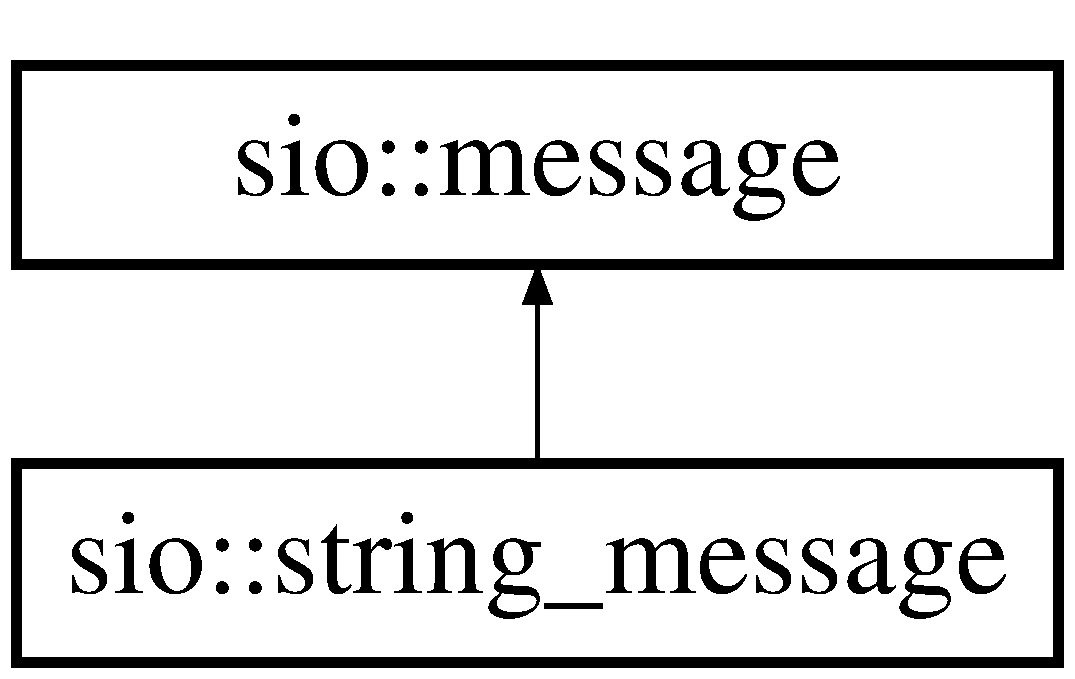
\includegraphics[height=2.000000cm]{classsio_1_1string__message}
\end{center}
\end{figure}
\doxysubsection*{Public Member Functions}
\begin{DoxyCompactItemize}
\item 
std\+::string const  \& \mbox{\hyperlink{classsio_1_1string__message_a8c79f0c15468e15251029c9f1612ca44}{get\+\_\+string}} () const
\end{DoxyCompactItemize}
\doxysubsection*{Static Public Member Functions}
\begin{DoxyCompactItemize}
\item 
static \mbox{\hyperlink{classsio_1_1message_a6340b6fef57e4516eb17928b1885a615}{message\+::ptr}} \mbox{\hyperlink{classsio_1_1string__message_a0614dc0722eacc4f40ac6dcbcc03b819}{create}} (std\+::string const \&v)
\item 
static \mbox{\hyperlink{classsio_1_1message_a6340b6fef57e4516eb17928b1885a615}{message\+::ptr}} \mbox{\hyperlink{classsio_1_1string__message_a91c0f23b04c84649b1a7ee8ed8351348}{create}} (std\+::string \&\&v)
\end{DoxyCompactItemize}
\doxysubsection*{Additional Inherited Members}


\doxysubsection{Member Function Documentation}
\mbox{\Hypertarget{classsio_1_1string__message_a91c0f23b04c84649b1a7ee8ed8351348}\label{classsio_1_1string__message_a91c0f23b04c84649b1a7ee8ed8351348}} 
\index{sio::string\_message@{sio::string\_message}!create@{create}}
\index{create@{create}!sio::string\_message@{sio::string\_message}}
\doxysubsubsection{\texorpdfstring{create()}{create()}\hspace{0.1cm}{\footnotesize\ttfamily [1/2]}}
{\footnotesize\ttfamily static \mbox{\hyperlink{classsio_1_1message_a6340b6fef57e4516eb17928b1885a615}{message\+::ptr}} sio\+::string\+\_\+message\+::create (\begin{DoxyParamCaption}\item[{std\+::string \&\&}]{v }\end{DoxyParamCaption})\hspace{0.3cm}{\ttfamily [inline]}, {\ttfamily [static]}}

\mbox{\Hypertarget{classsio_1_1string__message_a0614dc0722eacc4f40ac6dcbcc03b819}\label{classsio_1_1string__message_a0614dc0722eacc4f40ac6dcbcc03b819}} 
\index{sio::string\_message@{sio::string\_message}!create@{create}}
\index{create@{create}!sio::string\_message@{sio::string\_message}}
\doxysubsubsection{\texorpdfstring{create()}{create()}\hspace{0.1cm}{\footnotesize\ttfamily [2/2]}}
{\footnotesize\ttfamily static \mbox{\hyperlink{classsio_1_1message_a6340b6fef57e4516eb17928b1885a615}{message\+::ptr}} sio\+::string\+\_\+message\+::create (\begin{DoxyParamCaption}\item[{std\+::string const \&}]{v }\end{DoxyParamCaption})\hspace{0.3cm}{\ttfamily [inline]}, {\ttfamily [static]}}

\mbox{\Hypertarget{classsio_1_1string__message_a8c79f0c15468e15251029c9f1612ca44}\label{classsio_1_1string__message_a8c79f0c15468e15251029c9f1612ca44}} 
\index{sio::string\_message@{sio::string\_message}!get\_string@{get\_string}}
\index{get\_string@{get\_string}!sio::string\_message@{sio::string\_message}}
\doxysubsubsection{\texorpdfstring{get\_string()}{get\_string()}}
{\footnotesize\ttfamily std\+::string const\& sio\+::string\+\_\+message\+::get\+\_\+string (\begin{DoxyParamCaption}{ }\end{DoxyParamCaption}) const\hspace{0.3cm}{\ttfamily [inline]}, {\ttfamily [virtual]}}



Reimplemented from \mbox{\hyperlink{classsio_1_1message_a8e923d7e688e1bc69b586ef33684dd7a}{sio\+::message}}.



The documentation for this class was generated from the following file\+:\begin{DoxyCompactItemize}
\item 
/home/erik/work/bridges/bridges-\/cxx/src/\mbox{\hyperlink{sio__message_8h}{sio\+\_\+message.\+h}}\end{DoxyCompactItemize}

\hypertarget{classbridges_1_1datastructure_1_1_symbol}{}\section{bridges\+:\+:datastructure\+:\+:Symbol Class Reference}
\label{classbridges_1_1datastructure_1_1_symbol}\index{bridges\+::datastructure\+::\+Symbol@{bridges\+::datastructure\+::\+Symbol}}


{\ttfamily \#include $<$Symbol.\+h$>$}

Inheritance diagram for bridges\+:\+:datastructure\+:\+:Symbol\+:\begin{figure}[H]
\begin{center}
\leavevmode
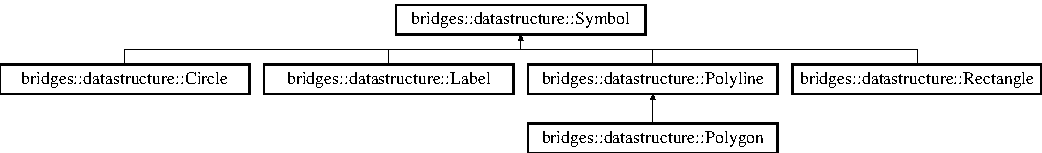
\includegraphics[height=2.058824cm]{classbridges_1_1datastructure_1_1_symbol}
\end{center}
\end{figure}


\subsection{Detailed Description}
This is an abstract class for deriving a number of \hyperlink{classbridges_1_1datastructure_1_1_symbol}{Symbol} shape objects, for use in a \hyperlink{classbridges_1_1datastructure_1_1_symbol_collection}{Symbol\+Collection}. Symbols correspond to a simplified subset of S\+VG paths and shapes for custom visual representations in B\+R\+I\+D\+G\+ES. 

Currently shapes supported are rectangle, circle, polygon, label; each shape has a name, location (x, y) and appropriate geometric and non-\/geometric attributes

\begin{DoxyAuthor}{Author}
David Burlinson, Kalpathi Subramanian 
\end{DoxyAuthor}
\begin{DoxyDate}{Date}
12/24/18, 7/12/19 
\end{DoxyDate}
\subsection*{Public Member Functions}
\begin{DoxyCompactItemize}
\item 
\hyperlink{classbridges_1_1datastructure_1_1_symbol_a6169106c021d20752abba3cd266ecfb0}{Symbol} ()
\item 
virtual const string \hyperlink{classbridges_1_1datastructure_1_1_symbol_a8044b3da559dcd9de8510ae339f126c8}{get\+Symbol\+Representation} () const =0
\item 
virtual vector$<$ float $>$ \hyperlink{classbridges_1_1datastructure_1_1_symbol_a37ba60b6acdd0888677eb8c64a931679}{get\+Dimensions} ()=0
\item 
\hyperlink{classbridges_1_1datastructure_1_1_symbol_adaeede160240bcc959d1813c5cb79528}{Symbol} (string symb)
\item 
int \hyperlink{classbridges_1_1datastructure_1_1_symbol_ac4b6cfcf91217d66ed0694080846970f}{get\+Identifier} ()
\item 
void \hyperlink{classbridges_1_1datastructure_1_1_symbol_a34609dd22e5043c39d40524d05e337b0}{set\+Label} (string lbl)
\item 
string \hyperlink{classbridges_1_1datastructure_1_1_symbol_a549906b96da5d53b964844ca5f593b7f}{get\+Label} () const
\item 
void \hyperlink{classbridges_1_1datastructure_1_1_symbol_a3019a17458fe5f0381cfd611338af6f7}{set\+Fill\+Color} (\hyperlink{classbridges_1_1datastructure_1_1_color}{Color} c)
\item 
void \hyperlink{classbridges_1_1datastructure_1_1_symbol_ad7b92720fe76b59f1922fe25c967f442}{set\+Fill\+Color} (string c)
\item 
\hyperlink{classbridges_1_1datastructure_1_1_color}{Color} \hyperlink{classbridges_1_1datastructure_1_1_symbol_a4b29601e24832077a15321af5c71cfdf}{get\+Fill\+Color} ()
\item 
void \hyperlink{classbridges_1_1datastructure_1_1_symbol_ad98bc6de925ff8ee2274298e42617fc8}{set\+Stroke\+Color} (\hyperlink{classbridges_1_1datastructure_1_1_color}{Color} c)
\item 
void \hyperlink{classbridges_1_1datastructure_1_1_symbol_af5f15111c67cfd63d3b0b3dc70442d0c}{set\+Stroke\+Color} (string c)
\item 
\hyperlink{classbridges_1_1datastructure_1_1_color}{Color} \hyperlink{classbridges_1_1datastructure_1_1_symbol_aa99d36f97deaf99bee1d61778c85e87d}{get\+Stroke\+Color} ()
\item 
void \hyperlink{classbridges_1_1datastructure_1_1_symbol_a56238a4535a26bc3eea698eea4b65921}{set\+Stroke\+Width} (float strk\+\_\+width)
\item 
float \hyperlink{classbridges_1_1datastructure_1_1_symbol_a4274feed56b8dfe89ffa3f791ece2ebd}{get\+Stroke\+Width} ()
\item 
void \hyperlink{classbridges_1_1datastructure_1_1_symbol_a889bace56d39df0ac09ba408ca868b7d}{set\+Opacity} (float op)
\item 
float \hyperlink{classbridges_1_1datastructure_1_1_symbol_af77f6e4c42ca97672888d863335b851a}{get\+Opacity} ()
\item 
void \hyperlink{classbridges_1_1datastructure_1_1_symbol_afd39d3b65d22bc2a1be64c8728f5e5d7}{set\+Stroke\+Dash} (int dash)
\item 
int \hyperlink{classbridges_1_1datastructure_1_1_symbol_a5fd32d1310c9ef97b07acab8efb17808}{get\+Stroke\+Dash} ()
\item 
void \hyperlink{classbridges_1_1datastructure_1_1_symbol_a9c62675b598fc5e755721576852f2dcf}{set\+Location} (int x, int y)
\item 
void \hyperlink{classbridges_1_1datastructure_1_1_symbol_a98a1c3d133e7fe2150d933495e421760}{set\+Center} (float x, float y)
\item 
void \hyperlink{classbridges_1_1datastructure_1_1_symbol_a4dbf51dac8b22b293a7061f5eb84b460}{set\+Location} (float x, float y)
\item 
float $\ast$ \hyperlink{classbridges_1_1datastructure_1_1_symbol_aeb4ec154605998d77dd9f96aa99ff16a}{get\+Location} ()
\item 
string \hyperlink{classbridges_1_1datastructure_1_1_symbol_a9365f8d91faf67e14ceaa89f8a5d0338}{get\+Name} () const
\end{DoxyCompactItemize}
\subsection*{Protected Member Functions}
\begin{DoxyCompactItemize}
\item 
void \hyperlink{classbridges_1_1datastructure_1_1_symbol_add56ff3bb5b276c016cfe377ff0f3fe2}{set\+Shape\+Type} (string s)
\begin{DoxyCompactList}\small\item\em Set the shape type. \end{DoxyCompactList}\item 
string \hyperlink{classbridges_1_1datastructure_1_1_symbol_a8f8378ed4009865611ce8b93e4432211}{get\+Shape\+Type} () const
\item 
void \hyperlink{classbridges_1_1datastructure_1_1_symbol_a3331549f82faa00d8fee5f51ca547cb0}{translate\+Point} (float $\ast$pt, float tx, float ty)
\begin{DoxyCompactList}\small\item\em Translate a 2D point. \end{DoxyCompactList}\item 
void \hyperlink{classbridges_1_1datastructure_1_1_symbol_ac27131f6461a763e55f1127f3cf87932}{scale\+Point} (float $\ast$pt, float sx, float sy)
\begin{DoxyCompactList}\small\item\em Scale a 2D point. \end{DoxyCompactList}\item 
void \hyperlink{classbridges_1_1datastructure_1_1_symbol_ad40678e04bae69b4c03881148678e71e}{rotate\+Point} (float $\ast$pt, float angle)
\begin{DoxyCompactList}\small\item\em Rotate a 2D point (about Z) \end{DoxyCompactList}\item 
const string \hyperlink{classbridges_1_1datastructure_1_1_symbol_ab9a92e73867a95e8cc3e63cad75d266a}{get\+Symbol\+Attribute\+Representation} () const
\end{DoxyCompactItemize}


\subsection{Constructor \& Destructor Documentation}
\mbox{\Hypertarget{classbridges_1_1datastructure_1_1_symbol_a6169106c021d20752abba3cd266ecfb0}\label{classbridges_1_1datastructure_1_1_symbol_a6169106c021d20752abba3cd266ecfb0}} 
\index{bridges\+::datastructure\+::\+Symbol@{bridges\+::datastructure\+::\+Symbol}!Symbol@{Symbol}}
\index{Symbol@{Symbol}!bridges\+::datastructure\+::\+Symbol@{bridges\+::datastructure\+::\+Symbol}}
\subsubsection{\texorpdfstring{Symbol()}{Symbol()}\hspace{0.1cm}{\footnotesize\ttfamily [1/2]}}
{\footnotesize\ttfamily bridges\+::datastructure\+::\+Symbol\+::\+Symbol (\begin{DoxyParamCaption}{ }\end{DoxyParamCaption})\hspace{0.3cm}{\ttfamily [inline]}}

\mbox{\Hypertarget{classbridges_1_1datastructure_1_1_symbol_adaeede160240bcc959d1813c5cb79528}\label{classbridges_1_1datastructure_1_1_symbol_adaeede160240bcc959d1813c5cb79528}} 
\index{bridges\+::datastructure\+::\+Symbol@{bridges\+::datastructure\+::\+Symbol}!Symbol@{Symbol}}
\index{Symbol@{Symbol}!bridges\+::datastructure\+::\+Symbol@{bridges\+::datastructure\+::\+Symbol}}
\subsubsection{\texorpdfstring{Symbol()}{Symbol()}\hspace{0.1cm}{\footnotesize\ttfamily [2/2]}}
{\footnotesize\ttfamily bridges\+::datastructure\+::\+Symbol\+::\+Symbol (\begin{DoxyParamCaption}\item[{string}]{symb }\end{DoxyParamCaption})\hspace{0.3cm}{\ttfamily [inline]}}

create a symbole of type \char`\"{}symb\char`\"{} 

\subsection{Member Function Documentation}
\mbox{\Hypertarget{classbridges_1_1datastructure_1_1_symbol_a37ba60b6acdd0888677eb8c64a931679}\label{classbridges_1_1datastructure_1_1_symbol_a37ba60b6acdd0888677eb8c64a931679}} 
\index{bridges\+::datastructure\+::\+Symbol@{bridges\+::datastructure\+::\+Symbol}!get\+Dimensions@{get\+Dimensions}}
\index{get\+Dimensions@{get\+Dimensions}!bridges\+::datastructure\+::\+Symbol@{bridges\+::datastructure\+::\+Symbol}}
\subsubsection{\texorpdfstring{get\+Dimensions()}{getDimensions()}}
{\footnotesize\ttfamily virtual vector$<$float$>$ bridges\+::datastructure\+::\+Symbol\+::get\+Dimensions (\begin{DoxyParamCaption}{ }\end{DoxyParamCaption})\hspace{0.3cm}{\ttfamily [pure virtual]}}

method to get the bounding box (dimensions) of the shape 

Implemented in \hyperlink{classbridges_1_1datastructure_1_1_polyline_aebcd7f4f80e2eed35057e5b1d82ba4e7}{bridges\+::datastructure\+::\+Polyline}, \hyperlink{classbridges_1_1datastructure_1_1_label_ac8f5e0d05c8f4466b3bf07e1fa342091}{bridges\+::datastructure\+::\+Label}, \hyperlink{classbridges_1_1datastructure_1_1_rectangle_a2afae03e3ddd9bebaed1e573e04bdbf3}{bridges\+::datastructure\+::\+Rectangle}, and \hyperlink{classbridges_1_1datastructure_1_1_circle_a4e08c866e2f10945c16921454d49a030}{bridges\+::datastructure\+::\+Circle}.

\mbox{\Hypertarget{classbridges_1_1datastructure_1_1_symbol_a4b29601e24832077a15321af5c71cfdf}\label{classbridges_1_1datastructure_1_1_symbol_a4b29601e24832077a15321af5c71cfdf}} 
\index{bridges\+::datastructure\+::\+Symbol@{bridges\+::datastructure\+::\+Symbol}!get\+Fill\+Color@{get\+Fill\+Color}}
\index{get\+Fill\+Color@{get\+Fill\+Color}!bridges\+::datastructure\+::\+Symbol@{bridges\+::datastructure\+::\+Symbol}}
\subsubsection{\texorpdfstring{get\+Fill\+Color()}{getFillColor()}}
{\footnotesize\ttfamily \hyperlink{classbridges_1_1datastructure_1_1_color}{Color} bridges\+::datastructure\+::\+Symbol\+::get\+Fill\+Color (\begin{DoxyParamCaption}{ }\end{DoxyParamCaption})\hspace{0.3cm}{\ttfamily [inline]}}

This method gets fill color

\begin{DoxyReturn}{Returns}
fill color 
\end{DoxyReturn}
\mbox{\Hypertarget{classbridges_1_1datastructure_1_1_symbol_ac4b6cfcf91217d66ed0694080846970f}\label{classbridges_1_1datastructure_1_1_symbol_ac4b6cfcf91217d66ed0694080846970f}} 
\index{bridges\+::datastructure\+::\+Symbol@{bridges\+::datastructure\+::\+Symbol}!get\+Identifier@{get\+Identifier}}
\index{get\+Identifier@{get\+Identifier}!bridges\+::datastructure\+::\+Symbol@{bridges\+::datastructure\+::\+Symbol}}
\subsubsection{\texorpdfstring{get\+Identifier()}{getIdentifier()}}
{\footnotesize\ttfamily int bridges\+::datastructure\+::\+Symbol\+::get\+Identifier (\begin{DoxyParamCaption}{ }\end{DoxyParamCaption})\hspace{0.3cm}{\ttfamily [inline]}}

Maintains unique identifiers of symbols and returns the \hyperlink{classbridges_1_1datastructure_1_1_symbol}{Symbol}\textquotesingle{}s unique identifier

\begin{DoxyReturn}{Returns}
the identifier 
\end{DoxyReturn}
\mbox{\Hypertarget{classbridges_1_1datastructure_1_1_symbol_a549906b96da5d53b964844ca5f593b7f}\label{classbridges_1_1datastructure_1_1_symbol_a549906b96da5d53b964844ca5f593b7f}} 
\index{bridges\+::datastructure\+::\+Symbol@{bridges\+::datastructure\+::\+Symbol}!get\+Label@{get\+Label}}
\index{get\+Label@{get\+Label}!bridges\+::datastructure\+::\+Symbol@{bridges\+::datastructure\+::\+Symbol}}
\subsubsection{\texorpdfstring{get\+Label()}{getLabel()}}
{\footnotesize\ttfamily string bridges\+::datastructure\+::\+Symbol\+::get\+Label (\begin{DoxyParamCaption}{ }\end{DoxyParamCaption}) const\hspace{0.3cm}{\ttfamily [inline]}}

Get the symbol label

\begin{DoxyReturn}{Returns}
the label 
\end{DoxyReturn}
\mbox{\Hypertarget{classbridges_1_1datastructure_1_1_symbol_aeb4ec154605998d77dd9f96aa99ff16a}\label{classbridges_1_1datastructure_1_1_symbol_aeb4ec154605998d77dd9f96aa99ff16a}} 
\index{bridges\+::datastructure\+::\+Symbol@{bridges\+::datastructure\+::\+Symbol}!get\+Location@{get\+Location}}
\index{get\+Location@{get\+Location}!bridges\+::datastructure\+::\+Symbol@{bridges\+::datastructure\+::\+Symbol}}
\subsubsection{\texorpdfstring{get\+Location()}{getLocation()}}
{\footnotesize\ttfamily float$\ast$ bridges\+::datastructure\+::\+Symbol\+::get\+Location (\begin{DoxyParamCaption}{ }\end{DoxyParamCaption})\hspace{0.3cm}{\ttfamily [inline]}}

This method gets the symbol location

\begin{DoxyReturn}{Returns}
location (x, y) of the symbol 
\end{DoxyReturn}
\mbox{\Hypertarget{classbridges_1_1datastructure_1_1_symbol_a9365f8d91faf67e14ceaa89f8a5d0338}\label{classbridges_1_1datastructure_1_1_symbol_a9365f8d91faf67e14ceaa89f8a5d0338}} 
\index{bridges\+::datastructure\+::\+Symbol@{bridges\+::datastructure\+::\+Symbol}!get\+Name@{get\+Name}}
\index{get\+Name@{get\+Name}!bridges\+::datastructure\+::\+Symbol@{bridges\+::datastructure\+::\+Symbol}}
\subsubsection{\texorpdfstring{get\+Name()}{getName()}}
{\footnotesize\ttfamily string bridges\+::datastructure\+::\+Symbol\+::get\+Name (\begin{DoxyParamCaption}{ }\end{DoxyParamCaption}) const\hspace{0.3cm}{\ttfamily [inline]}}

This method gets the name of the symbol

\begin{DoxyReturn}{Returns}
name shape name 
\end{DoxyReturn}
\mbox{\Hypertarget{classbridges_1_1datastructure_1_1_symbol_af77f6e4c42ca97672888d863335b851a}\label{classbridges_1_1datastructure_1_1_symbol_af77f6e4c42ca97672888d863335b851a}} 
\index{bridges\+::datastructure\+::\+Symbol@{bridges\+::datastructure\+::\+Symbol}!get\+Opacity@{get\+Opacity}}
\index{get\+Opacity@{get\+Opacity}!bridges\+::datastructure\+::\+Symbol@{bridges\+::datastructure\+::\+Symbol}}
\subsubsection{\texorpdfstring{get\+Opacity()}{getOpacity()}}
{\footnotesize\ttfamily float bridges\+::datastructure\+::\+Symbol\+::get\+Opacity (\begin{DoxyParamCaption}{ }\end{DoxyParamCaption})\hspace{0.3cm}{\ttfamily [inline]}}

This method gets symbol opacity

\begin{DoxyReturn}{Returns}
symbol opacity 
\end{DoxyReturn}
\mbox{\Hypertarget{classbridges_1_1datastructure_1_1_symbol_a8f8378ed4009865611ce8b93e4432211}\label{classbridges_1_1datastructure_1_1_symbol_a8f8378ed4009865611ce8b93e4432211}} 
\index{bridges\+::datastructure\+::\+Symbol@{bridges\+::datastructure\+::\+Symbol}!get\+Shape\+Type@{get\+Shape\+Type}}
\index{get\+Shape\+Type@{get\+Shape\+Type}!bridges\+::datastructure\+::\+Symbol@{bridges\+::datastructure\+::\+Symbol}}
\subsubsection{\texorpdfstring{get\+Shape\+Type()}{getShapeType()}}
{\footnotesize\ttfamily string bridges\+::datastructure\+::\+Symbol\+::get\+Shape\+Type (\begin{DoxyParamCaption}{ }\end{DoxyParamCaption}) const\hspace{0.3cm}{\ttfamily [inline]}, {\ttfamily [protected]}}

Get the symbol label

\begin{DoxyReturn}{Returns}
the shape type 
\end{DoxyReturn}
\mbox{\Hypertarget{classbridges_1_1datastructure_1_1_symbol_aa99d36f97deaf99bee1d61778c85e87d}\label{classbridges_1_1datastructure_1_1_symbol_aa99d36f97deaf99bee1d61778c85e87d}} 
\index{bridges\+::datastructure\+::\+Symbol@{bridges\+::datastructure\+::\+Symbol}!get\+Stroke\+Color@{get\+Stroke\+Color}}
\index{get\+Stroke\+Color@{get\+Stroke\+Color}!bridges\+::datastructure\+::\+Symbol@{bridges\+::datastructure\+::\+Symbol}}
\subsubsection{\texorpdfstring{get\+Stroke\+Color()}{getStrokeColor()}}
{\footnotesize\ttfamily \hyperlink{classbridges_1_1datastructure_1_1_color}{Color} bridges\+::datastructure\+::\+Symbol\+::get\+Stroke\+Color (\begin{DoxyParamCaption}{ }\end{DoxyParamCaption})\hspace{0.3cm}{\ttfamily [inline]}}

This method gets stroke color

\begin{DoxyReturn}{Returns}
stroke color 
\end{DoxyReturn}
\mbox{\Hypertarget{classbridges_1_1datastructure_1_1_symbol_a5fd32d1310c9ef97b07acab8efb17808}\label{classbridges_1_1datastructure_1_1_symbol_a5fd32d1310c9ef97b07acab8efb17808}} 
\index{bridges\+::datastructure\+::\+Symbol@{bridges\+::datastructure\+::\+Symbol}!get\+Stroke\+Dash@{get\+Stroke\+Dash}}
\index{get\+Stroke\+Dash@{get\+Stroke\+Dash}!bridges\+::datastructure\+::\+Symbol@{bridges\+::datastructure\+::\+Symbol}}
\subsubsection{\texorpdfstring{get\+Stroke\+Dash()}{getStrokeDash()}}
{\footnotesize\ttfamily int bridges\+::datastructure\+::\+Symbol\+::get\+Stroke\+Dash (\begin{DoxyParamCaption}{ }\end{DoxyParamCaption})\hspace{0.3cm}{\ttfamily [inline]}}

This method gets stroke dash level

\begin{DoxyReturn}{Returns}
stroke dash level 
\end{DoxyReturn}
\mbox{\Hypertarget{classbridges_1_1datastructure_1_1_symbol_a4274feed56b8dfe89ffa3f791ece2ebd}\label{classbridges_1_1datastructure_1_1_symbol_a4274feed56b8dfe89ffa3f791ece2ebd}} 
\index{bridges\+::datastructure\+::\+Symbol@{bridges\+::datastructure\+::\+Symbol}!get\+Stroke\+Width@{get\+Stroke\+Width}}
\index{get\+Stroke\+Width@{get\+Stroke\+Width}!bridges\+::datastructure\+::\+Symbol@{bridges\+::datastructure\+::\+Symbol}}
\subsubsection{\texorpdfstring{get\+Stroke\+Width()}{getStrokeWidth()}}
{\footnotesize\ttfamily float bridges\+::datastructure\+::\+Symbol\+::get\+Stroke\+Width (\begin{DoxyParamCaption}{ }\end{DoxyParamCaption})\hspace{0.3cm}{\ttfamily [inline]}}

This method gets stroke width

\begin{DoxyReturn}{Returns}
stroke width 
\end{DoxyReturn}
\mbox{\Hypertarget{classbridges_1_1datastructure_1_1_symbol_ab9a92e73867a95e8cc3e63cad75d266a}\label{classbridges_1_1datastructure_1_1_symbol_ab9a92e73867a95e8cc3e63cad75d266a}} 
\index{bridges\+::datastructure\+::\+Symbol@{bridges\+::datastructure\+::\+Symbol}!get\+Symbol\+Attribute\+Representation@{get\+Symbol\+Attribute\+Representation}}
\index{get\+Symbol\+Attribute\+Representation@{get\+Symbol\+Attribute\+Representation}!bridges\+::datastructure\+::\+Symbol@{bridges\+::datastructure\+::\+Symbol}}
\subsubsection{\texorpdfstring{get\+Symbol\+Attribute\+Representation()}{getSymbolAttributeRepresentation()}}
{\footnotesize\ttfamily const string bridges\+::datastructure\+::\+Symbol\+::get\+Symbol\+Attribute\+Representation (\begin{DoxyParamCaption}{ }\end{DoxyParamCaption}) const\hspace{0.3cm}{\ttfamily [inline]}, {\ttfamily [protected]}}

This method gets the J\+S\+ON representation of all of the symbol attributes

\begin{DoxyReturn}{Returns}
J\+S\+ON string of symbol attributes 
\end{DoxyReturn}
\mbox{\Hypertarget{classbridges_1_1datastructure_1_1_symbol_a8044b3da559dcd9de8510ae339f126c8}\label{classbridges_1_1datastructure_1_1_symbol_a8044b3da559dcd9de8510ae339f126c8}} 
\index{bridges\+::datastructure\+::\+Symbol@{bridges\+::datastructure\+::\+Symbol}!get\+Symbol\+Representation@{get\+Symbol\+Representation}}
\index{get\+Symbol\+Representation@{get\+Symbol\+Representation}!bridges\+::datastructure\+::\+Symbol@{bridges\+::datastructure\+::\+Symbol}}
\subsubsection{\texorpdfstring{get\+Symbol\+Representation()}{getSymbolRepresentation()}}
{\footnotesize\ttfamily virtual const string bridges\+::datastructure\+::\+Symbol\+::get\+Symbol\+Representation (\begin{DoxyParamCaption}{ }\end{DoxyParamCaption}) const\hspace{0.3cm}{\ttfamily [pure virtual]}}

virtual Method to get the J\+S\+ON representation of the symbol 

Implemented in \hyperlink{classbridges_1_1datastructure_1_1_polyline_a176c06400a3b105fa651c69891381201}{bridges\+::datastructure\+::\+Polyline}, \hyperlink{classbridges_1_1datastructure_1_1_rectangle_ada89ed40d2515a3518084f5460ba8dac}{bridges\+::datastructure\+::\+Rectangle}, \hyperlink{classbridges_1_1datastructure_1_1_label_aa3b7c9e5630ecc8a2534e6db2a220e90}{bridges\+::datastructure\+::\+Label}, and \hyperlink{classbridges_1_1datastructure_1_1_circle_a796c88ccb8c5529d45aa7271a34fa3fe}{bridges\+::datastructure\+::\+Circle}.

\mbox{\Hypertarget{classbridges_1_1datastructure_1_1_symbol_ad40678e04bae69b4c03881148678e71e}\label{classbridges_1_1datastructure_1_1_symbol_ad40678e04bae69b4c03881148678e71e}} 
\index{bridges\+::datastructure\+::\+Symbol@{bridges\+::datastructure\+::\+Symbol}!rotate\+Point@{rotate\+Point}}
\index{rotate\+Point@{rotate\+Point}!bridges\+::datastructure\+::\+Symbol@{bridges\+::datastructure\+::\+Symbol}}
\subsubsection{\texorpdfstring{rotate\+Point()}{rotatePoint()}}
{\footnotesize\ttfamily void bridges\+::datastructure\+::\+Symbol\+::rotate\+Point (\begin{DoxyParamCaption}\item[{float $\ast$}]{pt,  }\item[{float}]{angle }\end{DoxyParamCaption})\hspace{0.3cm}{\ttfamily [inline]}, {\ttfamily [protected]}}



Rotate a 2D point (about Z) 


\begin{DoxyParams}{Parameters}
{\em pt} & 2D point (x, y) \\
\hline
{\em angle} & rotation angle in degrees (positive is counter clockwise, negative is clockwise) \\
\hline
\end{DoxyParams}
\mbox{\Hypertarget{classbridges_1_1datastructure_1_1_symbol_ac27131f6461a763e55f1127f3cf87932}\label{classbridges_1_1datastructure_1_1_symbol_ac27131f6461a763e55f1127f3cf87932}} 
\index{bridges\+::datastructure\+::\+Symbol@{bridges\+::datastructure\+::\+Symbol}!scale\+Point@{scale\+Point}}
\index{scale\+Point@{scale\+Point}!bridges\+::datastructure\+::\+Symbol@{bridges\+::datastructure\+::\+Symbol}}
\subsubsection{\texorpdfstring{scale\+Point()}{scalePoint()}}
{\footnotesize\ttfamily void bridges\+::datastructure\+::\+Symbol\+::scale\+Point (\begin{DoxyParamCaption}\item[{float $\ast$}]{pt,  }\item[{float}]{sx,  }\item[{float}]{sy }\end{DoxyParamCaption})\hspace{0.3cm}{\ttfamily [inline]}, {\ttfamily [protected]}}



Scale a 2D point. 


\begin{DoxyParams}{Parameters}
{\em pt} & 2D point (x, y) \\
\hline
{\em sx,sy} & scale factors along each axis \\
\hline
\end{DoxyParams}
\mbox{\Hypertarget{classbridges_1_1datastructure_1_1_symbol_a98a1c3d133e7fe2150d933495e421760}\label{classbridges_1_1datastructure_1_1_symbol_a98a1c3d133e7fe2150d933495e421760}} 
\index{bridges\+::datastructure\+::\+Symbol@{bridges\+::datastructure\+::\+Symbol}!set\+Center@{set\+Center}}
\index{set\+Center@{set\+Center}!bridges\+::datastructure\+::\+Symbol@{bridges\+::datastructure\+::\+Symbol}}
\subsubsection{\texorpdfstring{set\+Center()}{setCenter()}}
{\footnotesize\ttfamily void bridges\+::datastructure\+::\+Symbol\+::set\+Center (\begin{DoxyParamCaption}\item[{float}]{x,  }\item[{float}]{y }\end{DoxyParamCaption})\hspace{0.3cm}{\ttfamily [inline]}}

This method sets the symbol location


\begin{DoxyParams}{Parameters}
{\em x} & x coordinate \\
\hline
{\em y} & y coordinate \\
\hline
\end{DoxyParams}
\mbox{\Hypertarget{classbridges_1_1datastructure_1_1_symbol_a3019a17458fe5f0381cfd611338af6f7}\label{classbridges_1_1datastructure_1_1_symbol_a3019a17458fe5f0381cfd611338af6f7}} 
\index{bridges\+::datastructure\+::\+Symbol@{bridges\+::datastructure\+::\+Symbol}!set\+Fill\+Color@{set\+Fill\+Color}}
\index{set\+Fill\+Color@{set\+Fill\+Color}!bridges\+::datastructure\+::\+Symbol@{bridges\+::datastructure\+::\+Symbol}}
\subsubsection{\texorpdfstring{set\+Fill\+Color()}{setFillColor()}\hspace{0.1cm}{\footnotesize\ttfamily [1/2]}}
{\footnotesize\ttfamily void bridges\+::datastructure\+::\+Symbol\+::set\+Fill\+Color (\begin{DoxyParamCaption}\item[{\hyperlink{classbridges_1_1datastructure_1_1_color}{Color}}]{c }\end{DoxyParamCaption})\hspace{0.3cm}{\ttfamily [inline]}}

This method sets the symbol fill color


\begin{DoxyParams}{Parameters}
{\em c} & the color to set \\
\hline
\end{DoxyParams}
\mbox{\Hypertarget{classbridges_1_1datastructure_1_1_symbol_ad7b92720fe76b59f1922fe25c967f442}\label{classbridges_1_1datastructure_1_1_symbol_ad7b92720fe76b59f1922fe25c967f442}} 
\index{bridges\+::datastructure\+::\+Symbol@{bridges\+::datastructure\+::\+Symbol}!set\+Fill\+Color@{set\+Fill\+Color}}
\index{set\+Fill\+Color@{set\+Fill\+Color}!bridges\+::datastructure\+::\+Symbol@{bridges\+::datastructure\+::\+Symbol}}
\subsubsection{\texorpdfstring{set\+Fill\+Color()}{setFillColor()}\hspace{0.1cm}{\footnotesize\ttfamily [2/2]}}
{\footnotesize\ttfamily void bridges\+::datastructure\+::\+Symbol\+::set\+Fill\+Color (\begin{DoxyParamCaption}\item[{string}]{c }\end{DoxyParamCaption})\hspace{0.3cm}{\ttfamily [inline]}}

This method sets the symbol fill color


\begin{DoxyParams}{Parameters}
{\em c} & the named color to set \\
\hline
\end{DoxyParams}
\mbox{\Hypertarget{classbridges_1_1datastructure_1_1_symbol_a34609dd22e5043c39d40524d05e337b0}\label{classbridges_1_1datastructure_1_1_symbol_a34609dd22e5043c39d40524d05e337b0}} 
\index{bridges\+::datastructure\+::\+Symbol@{bridges\+::datastructure\+::\+Symbol}!set\+Label@{set\+Label}}
\index{set\+Label@{set\+Label}!bridges\+::datastructure\+::\+Symbol@{bridges\+::datastructure\+::\+Symbol}}
\subsubsection{\texorpdfstring{set\+Label()}{setLabel()}}
{\footnotesize\ttfamily void bridges\+::datastructure\+::\+Symbol\+::set\+Label (\begin{DoxyParamCaption}\item[{string}]{lbl }\end{DoxyParamCaption})\hspace{0.3cm}{\ttfamily [inline]}}

This method sets the symbol label


\begin{DoxyParams}{Parameters}
{\em lbl} & the label to set \\
\hline
\end{DoxyParams}
\mbox{\Hypertarget{classbridges_1_1datastructure_1_1_symbol_a9c62675b598fc5e755721576852f2dcf}\label{classbridges_1_1datastructure_1_1_symbol_a9c62675b598fc5e755721576852f2dcf}} 
\index{bridges\+::datastructure\+::\+Symbol@{bridges\+::datastructure\+::\+Symbol}!set\+Location@{set\+Location}}
\index{set\+Location@{set\+Location}!bridges\+::datastructure\+::\+Symbol@{bridges\+::datastructure\+::\+Symbol}}
\subsubsection{\texorpdfstring{set\+Location()}{setLocation()}\hspace{0.1cm}{\footnotesize\ttfamily [1/2]}}
{\footnotesize\ttfamily void bridges\+::datastructure\+::\+Symbol\+::set\+Location (\begin{DoxyParamCaption}\item[{int}]{x,  }\item[{int}]{y }\end{DoxyParamCaption})\hspace{0.3cm}{\ttfamily [inline]}}

This method sets the symbol location


\begin{DoxyParams}{Parameters}
{\em x} & x coordinate \\
\hline
{\em y} & y coordinate \\
\hline
\end{DoxyParams}
\mbox{\Hypertarget{classbridges_1_1datastructure_1_1_symbol_a4dbf51dac8b22b293a7061f5eb84b460}\label{classbridges_1_1datastructure_1_1_symbol_a4dbf51dac8b22b293a7061f5eb84b460}} 
\index{bridges\+::datastructure\+::\+Symbol@{bridges\+::datastructure\+::\+Symbol}!set\+Location@{set\+Location}}
\index{set\+Location@{set\+Location}!bridges\+::datastructure\+::\+Symbol@{bridges\+::datastructure\+::\+Symbol}}
\subsubsection{\texorpdfstring{set\+Location()}{setLocation()}\hspace{0.1cm}{\footnotesize\ttfamily [2/2]}}
{\footnotesize\ttfamily void bridges\+::datastructure\+::\+Symbol\+::set\+Location (\begin{DoxyParamCaption}\item[{float}]{x,  }\item[{float}]{y }\end{DoxyParamCaption})\hspace{0.3cm}{\ttfamily [inline]}}

This method sets the ssymbol location


\begin{DoxyParams}{Parameters}
{\em x} & x coordinate \\
\hline
{\em y} & y coordinate \\
\hline
\end{DoxyParams}
\mbox{\Hypertarget{classbridges_1_1datastructure_1_1_symbol_a889bace56d39df0ac09ba408ca868b7d}\label{classbridges_1_1datastructure_1_1_symbol_a889bace56d39df0ac09ba408ca868b7d}} 
\index{bridges\+::datastructure\+::\+Symbol@{bridges\+::datastructure\+::\+Symbol}!set\+Opacity@{set\+Opacity}}
\index{set\+Opacity@{set\+Opacity}!bridges\+::datastructure\+::\+Symbol@{bridges\+::datastructure\+::\+Symbol}}
\subsubsection{\texorpdfstring{set\+Opacity()}{setOpacity()}}
{\footnotesize\ttfamily void bridges\+::datastructure\+::\+Symbol\+::set\+Opacity (\begin{DoxyParamCaption}\item[{float}]{op }\end{DoxyParamCaption})\hspace{0.3cm}{\ttfamily [inline]}}

This method sets the symbol opacity


\begin{DoxyParams}{Parameters}
{\em op} & the opacity to set \\
\hline
\end{DoxyParams}
\mbox{\Hypertarget{classbridges_1_1datastructure_1_1_symbol_add56ff3bb5b276c016cfe377ff0f3fe2}\label{classbridges_1_1datastructure_1_1_symbol_add56ff3bb5b276c016cfe377ff0f3fe2}} 
\index{bridges\+::datastructure\+::\+Symbol@{bridges\+::datastructure\+::\+Symbol}!set\+Shape\+Type@{set\+Shape\+Type}}
\index{set\+Shape\+Type@{set\+Shape\+Type}!bridges\+::datastructure\+::\+Symbol@{bridges\+::datastructure\+::\+Symbol}}
\subsubsection{\texorpdfstring{set\+Shape\+Type()}{setShapeType()}}
{\footnotesize\ttfamily void bridges\+::datastructure\+::\+Symbol\+::set\+Shape\+Type (\begin{DoxyParamCaption}\item[{string}]{s }\end{DoxyParamCaption})\hspace{0.3cm}{\ttfamily [inline]}, {\ttfamily [protected]}}



Set the shape type. 


\begin{DoxyParams}{Parameters}
{\em s} & shape type to set \\
\hline
\end{DoxyParams}
\mbox{\Hypertarget{classbridges_1_1datastructure_1_1_symbol_ad98bc6de925ff8ee2274298e42617fc8}\label{classbridges_1_1datastructure_1_1_symbol_ad98bc6de925ff8ee2274298e42617fc8}} 
\index{bridges\+::datastructure\+::\+Symbol@{bridges\+::datastructure\+::\+Symbol}!set\+Stroke\+Color@{set\+Stroke\+Color}}
\index{set\+Stroke\+Color@{set\+Stroke\+Color}!bridges\+::datastructure\+::\+Symbol@{bridges\+::datastructure\+::\+Symbol}}
\subsubsection{\texorpdfstring{set\+Stroke\+Color()}{setStrokeColor()}\hspace{0.1cm}{\footnotesize\ttfamily [1/2]}}
{\footnotesize\ttfamily void bridges\+::datastructure\+::\+Symbol\+::set\+Stroke\+Color (\begin{DoxyParamCaption}\item[{\hyperlink{classbridges_1_1datastructure_1_1_color}{Color}}]{c }\end{DoxyParamCaption})\hspace{0.3cm}{\ttfamily [inline]}}

This method sets the symbol stroke color


\begin{DoxyParams}{Parameters}
{\em c} & the color to set \\
\hline
\end{DoxyParams}
\mbox{\Hypertarget{classbridges_1_1datastructure_1_1_symbol_af5f15111c67cfd63d3b0b3dc70442d0c}\label{classbridges_1_1datastructure_1_1_symbol_af5f15111c67cfd63d3b0b3dc70442d0c}} 
\index{bridges\+::datastructure\+::\+Symbol@{bridges\+::datastructure\+::\+Symbol}!set\+Stroke\+Color@{set\+Stroke\+Color}}
\index{set\+Stroke\+Color@{set\+Stroke\+Color}!bridges\+::datastructure\+::\+Symbol@{bridges\+::datastructure\+::\+Symbol}}
\subsubsection{\texorpdfstring{set\+Stroke\+Color()}{setStrokeColor()}\hspace{0.1cm}{\footnotesize\ttfamily [2/2]}}
{\footnotesize\ttfamily void bridges\+::datastructure\+::\+Symbol\+::set\+Stroke\+Color (\begin{DoxyParamCaption}\item[{string}]{c }\end{DoxyParamCaption})\hspace{0.3cm}{\ttfamily [inline]}}

This method sets the symbol stroke color


\begin{DoxyParams}{Parameters}
{\em c} & the named color to set \\
\hline
\end{DoxyParams}
\mbox{\Hypertarget{classbridges_1_1datastructure_1_1_symbol_afd39d3b65d22bc2a1be64c8728f5e5d7}\label{classbridges_1_1datastructure_1_1_symbol_afd39d3b65d22bc2a1be64c8728f5e5d7}} 
\index{bridges\+::datastructure\+::\+Symbol@{bridges\+::datastructure\+::\+Symbol}!set\+Stroke\+Dash@{set\+Stroke\+Dash}}
\index{set\+Stroke\+Dash@{set\+Stroke\+Dash}!bridges\+::datastructure\+::\+Symbol@{bridges\+::datastructure\+::\+Symbol}}
\subsubsection{\texorpdfstring{set\+Stroke\+Dash()}{setStrokeDash()}}
{\footnotesize\ttfamily void bridges\+::datastructure\+::\+Symbol\+::set\+Stroke\+Dash (\begin{DoxyParamCaption}\item[{int}]{dash }\end{DoxyParamCaption})\hspace{0.3cm}{\ttfamily [inline]}}

This method sets the stroke dash level


\begin{DoxyParams}{Parameters}
{\em dash} & dash level \\
\hline
\end{DoxyParams}
\mbox{\Hypertarget{classbridges_1_1datastructure_1_1_symbol_a56238a4535a26bc3eea698eea4b65921}\label{classbridges_1_1datastructure_1_1_symbol_a56238a4535a26bc3eea698eea4b65921}} 
\index{bridges\+::datastructure\+::\+Symbol@{bridges\+::datastructure\+::\+Symbol}!set\+Stroke\+Width@{set\+Stroke\+Width}}
\index{set\+Stroke\+Width@{set\+Stroke\+Width}!bridges\+::datastructure\+::\+Symbol@{bridges\+::datastructure\+::\+Symbol}}
\subsubsection{\texorpdfstring{set\+Stroke\+Width()}{setStrokeWidth()}}
{\footnotesize\ttfamily void bridges\+::datastructure\+::\+Symbol\+::set\+Stroke\+Width (\begin{DoxyParamCaption}\item[{float}]{strk\+\_\+width }\end{DoxyParamCaption})\hspace{0.3cm}{\ttfamily [inline]}}

This method sets the symbol stroke width


\begin{DoxyParams}{Parameters}
{\em strk\+\_\+width} & the stroke width to set \\
\hline
\end{DoxyParams}
\mbox{\Hypertarget{classbridges_1_1datastructure_1_1_symbol_a3331549f82faa00d8fee5f51ca547cb0}\label{classbridges_1_1datastructure_1_1_symbol_a3331549f82faa00d8fee5f51ca547cb0}} 
\index{bridges\+::datastructure\+::\+Symbol@{bridges\+::datastructure\+::\+Symbol}!translate\+Point@{translate\+Point}}
\index{translate\+Point@{translate\+Point}!bridges\+::datastructure\+::\+Symbol@{bridges\+::datastructure\+::\+Symbol}}
\subsubsection{\texorpdfstring{translate\+Point()}{translatePoint()}}
{\footnotesize\ttfamily void bridges\+::datastructure\+::\+Symbol\+::translate\+Point (\begin{DoxyParamCaption}\item[{float $\ast$}]{pt,  }\item[{float}]{tx,  }\item[{float}]{ty }\end{DoxyParamCaption})\hspace{0.3cm}{\ttfamily [inline]}, {\ttfamily [protected]}}



Translate a 2D point. 


\begin{DoxyParams}{Parameters}
{\em pt} & 2D point (x, y) \\
\hline
{\em tx,ty} & translation vector \\
\hline
\end{DoxyParams}


The documentation for this class was generated from the following file\+:\begin{DoxyCompactItemize}
\item 
/home/erik/work/bridges/bridges-\/cxx/src/\hyperlink{_symbol_8h}{Symbol.\+h}\end{DoxyCompactItemize}

\hypertarget{classbridges_1_1datastructure_1_1_symbol_collection}{}\section{bridges\+:\+:datastructure\+:\+:Symbol\+Collection Class Reference}
\label{classbridges_1_1datastructure_1_1_symbol_collection}\index{bridges\+::datastructure\+::\+Symbol\+Collection@{bridges\+::datastructure\+::\+Symbol\+Collection}}


{\ttfamily \#include $<$Symbol\+Collection.\+h$>$}

Inheritance diagram for bridges\+:\+:datastructure\+:\+:Symbol\+Collection\+:\begin{figure}[H]
\begin{center}
\leavevmode
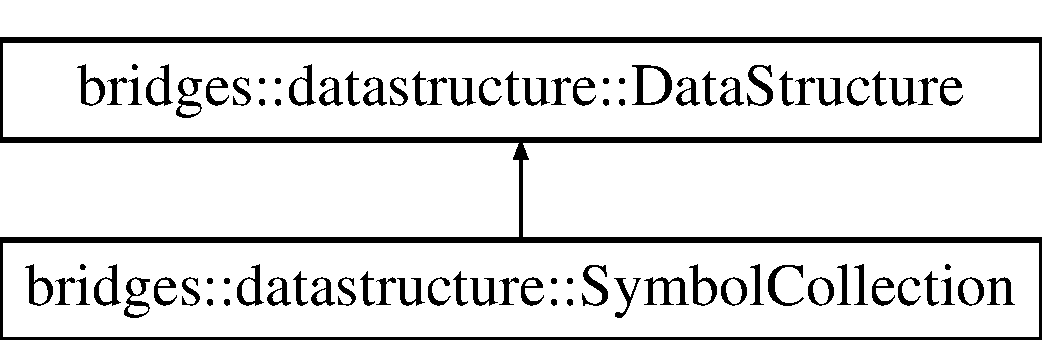
\includegraphics[height=2.000000cm]{classbridges_1_1datastructure_1_1_symbol_collection}
\end{center}
\end{figure}


\subsection{Detailed Description}
the Shape\+Collection represents a collection of symbols (shapes, polygons, and text) to visualize in \hyperlink{classbridges_1_1_bridges}{Bridges} 

\begin{DoxyAuthor}{Author}
Kalpathi Subramanian 
\end{DoxyAuthor}
\begin{DoxyDate}{Date}
10/9/18, 7/12/19 
\end{DoxyDate}
\subsection*{Public Member Functions}
\begin{DoxyCompactItemize}
\item 
void \hyperlink{classbridges_1_1datastructure_1_1_symbol_collection_a8853f758e4e8ab7f9cef5bf4d0494027}{set\+Viewport} (float xmin, float xmax, float ymin, float ymax)
\item 
\hyperlink{classbridges_1_1datastructure_1_1_symbol_collection_aa8d074ecf235848f4253b19d6f5c7c74}{Symbol\+Collection} ()
\item 
virtual const string \hyperlink{classbridges_1_1datastructure_1_1_symbol_collection_a8f63c31a48a12127978967b706fc38f5}{get\+D\+Stype} () const
\begin{DoxyCompactList}\small\item\em This method gets the data structure type. \end{DoxyCompactList}\item 
void \hyperlink{classbridges_1_1datastructure_1_1_symbol_collection_a14652e01cc99fc470f1fbea30d851a4f}{add\+Symbol} (\hyperlink{classbridges_1_1datastructure_1_1_symbol}{Symbol} \&s)
\begin{DoxyCompactList}\small\item\em This method adds a symbol to the collection. \end{DoxyCompactList}\end{DoxyCompactItemize}
\subsection*{Protected Attributes}
\begin{DoxyCompactItemize}
\item 
float \hyperlink{classbridges_1_1datastructure_1_1_symbol_collection_a3db2f9c5d239e4ca964ea017a2beedac}{domainxmin} = -\/100.\+0f
\item 
float \hyperlink{classbridges_1_1datastructure_1_1_symbol_collection_a424f539a0a7cc48735f58978bb37249b}{domainxmax} = 100.\+0f
\item 
float \hyperlink{classbridges_1_1datastructure_1_1_symbol_collection_a2f08353c46444762f329bec94f087a2b}{domainymin} = -\/100.\+0f
\item 
float \hyperlink{classbridges_1_1datastructure_1_1_symbol_collection_a62b61a0ec9546c68f31a324ff6e6b518}{domainymax} = 100.\+0f
\item 
bool \hyperlink{classbridges_1_1datastructure_1_1_symbol_collection_a27dc0406085568b06244bcc0f8957f68}{autoscaledomain} = true
\end{DoxyCompactItemize}


\subsection{Constructor \& Destructor Documentation}
\mbox{\Hypertarget{classbridges_1_1datastructure_1_1_symbol_collection_aa8d074ecf235848f4253b19d6f5c7c74}\label{classbridges_1_1datastructure_1_1_symbol_collection_aa8d074ecf235848f4253b19d6f5c7c74}} 
\index{bridges\+::datastructure\+::\+Symbol\+Collection@{bridges\+::datastructure\+::\+Symbol\+Collection}!Symbol\+Collection@{Symbol\+Collection}}
\index{Symbol\+Collection@{Symbol\+Collection}!bridges\+::datastructure\+::\+Symbol\+Collection@{bridges\+::datastructure\+::\+Symbol\+Collection}}
\subsubsection{\texorpdfstring{Symbol\+Collection()}{SymbolCollection()}}
{\footnotesize\ttfamily bridges\+::datastructure\+::\+Symbol\+Collection\+::\+Symbol\+Collection (\begin{DoxyParamCaption}{ }\end{DoxyParamCaption})\hspace{0.3cm}{\ttfamily [inline]}}

Constructor 

\subsection{Member Function Documentation}
\mbox{\Hypertarget{classbridges_1_1datastructure_1_1_symbol_collection_a14652e01cc99fc470f1fbea30d851a4f}\label{classbridges_1_1datastructure_1_1_symbol_collection_a14652e01cc99fc470f1fbea30d851a4f}} 
\index{bridges\+::datastructure\+::\+Symbol\+Collection@{bridges\+::datastructure\+::\+Symbol\+Collection}!add\+Symbol@{add\+Symbol}}
\index{add\+Symbol@{add\+Symbol}!bridges\+::datastructure\+::\+Symbol\+Collection@{bridges\+::datastructure\+::\+Symbol\+Collection}}
\subsubsection{\texorpdfstring{add\+Symbol()}{addSymbol()}}
{\footnotesize\ttfamily void bridges\+::datastructure\+::\+Symbol\+Collection\+::add\+Symbol (\begin{DoxyParamCaption}\item[{\hyperlink{classbridges_1_1datastructure_1_1_symbol}{Symbol} \&}]{s }\end{DoxyParamCaption})\hspace{0.3cm}{\ttfamily [inline]}}



This method adds a symbol to the collection. 


\begin{DoxyParams}{Parameters}
{\em s} & symbol being added \\
\hline
\end{DoxyParams}
\mbox{\Hypertarget{classbridges_1_1datastructure_1_1_symbol_collection_a8f63c31a48a12127978967b706fc38f5}\label{classbridges_1_1datastructure_1_1_symbol_collection_a8f63c31a48a12127978967b706fc38f5}} 
\index{bridges\+::datastructure\+::\+Symbol\+Collection@{bridges\+::datastructure\+::\+Symbol\+Collection}!get\+D\+Stype@{get\+D\+Stype}}
\index{get\+D\+Stype@{get\+D\+Stype}!bridges\+::datastructure\+::\+Symbol\+Collection@{bridges\+::datastructure\+::\+Symbol\+Collection}}
\subsubsection{\texorpdfstring{get\+D\+Stype()}{getDStype()}}
{\footnotesize\ttfamily virtual const string bridges\+::datastructure\+::\+Symbol\+Collection\+::get\+D\+Stype (\begin{DoxyParamCaption}{ }\end{DoxyParamCaption}) const\hspace{0.3cm}{\ttfamily [inline]}, {\ttfamily [virtual]}}



This method gets the data structure type. 

\begin{DoxyReturn}{Returns}
The date structure type as a string 
\end{DoxyReturn}


Implements \hyperlink{classbridges_1_1datastructure_1_1_data_structure_a4ff66cb34409f11fe9fc647f6d8a22ce}{bridges\+::datastructure\+::\+Data\+Structure}.

\mbox{\Hypertarget{classbridges_1_1datastructure_1_1_symbol_collection_a8853f758e4e8ab7f9cef5bf4d0494027}\label{classbridges_1_1datastructure_1_1_symbol_collection_a8853f758e4e8ab7f9cef5bf4d0494027}} 
\index{bridges\+::datastructure\+::\+Symbol\+Collection@{bridges\+::datastructure\+::\+Symbol\+Collection}!set\+Viewport@{set\+Viewport}}
\index{set\+Viewport@{set\+Viewport}!bridges\+::datastructure\+::\+Symbol\+Collection@{bridges\+::datastructure\+::\+Symbol\+Collection}}
\subsubsection{\texorpdfstring{set\+Viewport()}{setViewport()}}
{\footnotesize\ttfamily void bridges\+::datastructure\+::\+Symbol\+Collection\+::set\+Viewport (\begin{DoxyParamCaption}\item[{float}]{xmin,  }\item[{float}]{xmax,  }\item[{float}]{ymin,  }\item[{float}]{ymax }\end{DoxyParamCaption})\hspace{0.3cm}{\ttfamily [inline]}}



\subsection{Member Data Documentation}
\mbox{\Hypertarget{classbridges_1_1datastructure_1_1_symbol_collection_a27dc0406085568b06244bcc0f8957f68}\label{classbridges_1_1datastructure_1_1_symbol_collection_a27dc0406085568b06244bcc0f8957f68}} 
\index{bridges\+::datastructure\+::\+Symbol\+Collection@{bridges\+::datastructure\+::\+Symbol\+Collection}!autoscaledomain@{autoscaledomain}}
\index{autoscaledomain@{autoscaledomain}!bridges\+::datastructure\+::\+Symbol\+Collection@{bridges\+::datastructure\+::\+Symbol\+Collection}}
\subsubsection{\texorpdfstring{autoscaledomain}{autoscaledomain}}
{\footnotesize\ttfamily bool bridges\+::datastructure\+::\+Symbol\+Collection\+::autoscaledomain = true\hspace{0.3cm}{\ttfamily [protected]}}

\mbox{\Hypertarget{classbridges_1_1datastructure_1_1_symbol_collection_a424f539a0a7cc48735f58978bb37249b}\label{classbridges_1_1datastructure_1_1_symbol_collection_a424f539a0a7cc48735f58978bb37249b}} 
\index{bridges\+::datastructure\+::\+Symbol\+Collection@{bridges\+::datastructure\+::\+Symbol\+Collection}!domainxmax@{domainxmax}}
\index{domainxmax@{domainxmax}!bridges\+::datastructure\+::\+Symbol\+Collection@{bridges\+::datastructure\+::\+Symbol\+Collection}}
\subsubsection{\texorpdfstring{domainxmax}{domainxmax}}
{\footnotesize\ttfamily float bridges\+::datastructure\+::\+Symbol\+Collection\+::domainxmax = 100.\+0f\hspace{0.3cm}{\ttfamily [mutable]}, {\ttfamily [protected]}}

\mbox{\Hypertarget{classbridges_1_1datastructure_1_1_symbol_collection_a3db2f9c5d239e4ca964ea017a2beedac}\label{classbridges_1_1datastructure_1_1_symbol_collection_a3db2f9c5d239e4ca964ea017a2beedac}} 
\index{bridges\+::datastructure\+::\+Symbol\+Collection@{bridges\+::datastructure\+::\+Symbol\+Collection}!domainxmin@{domainxmin}}
\index{domainxmin@{domainxmin}!bridges\+::datastructure\+::\+Symbol\+Collection@{bridges\+::datastructure\+::\+Symbol\+Collection}}
\subsubsection{\texorpdfstring{domainxmin}{domainxmin}}
{\footnotesize\ttfamily float bridges\+::datastructure\+::\+Symbol\+Collection\+::domainxmin = -\/100.\+0f\hspace{0.3cm}{\ttfamily [mutable]}, {\ttfamily [protected]}}

\mbox{\Hypertarget{classbridges_1_1datastructure_1_1_symbol_collection_a62b61a0ec9546c68f31a324ff6e6b518}\label{classbridges_1_1datastructure_1_1_symbol_collection_a62b61a0ec9546c68f31a324ff6e6b518}} 
\index{bridges\+::datastructure\+::\+Symbol\+Collection@{bridges\+::datastructure\+::\+Symbol\+Collection}!domainymax@{domainymax}}
\index{domainymax@{domainymax}!bridges\+::datastructure\+::\+Symbol\+Collection@{bridges\+::datastructure\+::\+Symbol\+Collection}}
\subsubsection{\texorpdfstring{domainymax}{domainymax}}
{\footnotesize\ttfamily float bridges\+::datastructure\+::\+Symbol\+Collection\+::domainymax = 100.\+0f\hspace{0.3cm}{\ttfamily [mutable]}, {\ttfamily [protected]}}

\mbox{\Hypertarget{classbridges_1_1datastructure_1_1_symbol_collection_a2f08353c46444762f329bec94f087a2b}\label{classbridges_1_1datastructure_1_1_symbol_collection_a2f08353c46444762f329bec94f087a2b}} 
\index{bridges\+::datastructure\+::\+Symbol\+Collection@{bridges\+::datastructure\+::\+Symbol\+Collection}!domainymin@{domainymin}}
\index{domainymin@{domainymin}!bridges\+::datastructure\+::\+Symbol\+Collection@{bridges\+::datastructure\+::\+Symbol\+Collection}}
\subsubsection{\texorpdfstring{domainymin}{domainymin}}
{\footnotesize\ttfamily float bridges\+::datastructure\+::\+Symbol\+Collection\+::domainymin = -\/100.\+0f\hspace{0.3cm}{\ttfamily [mutable]}, {\ttfamily [protected]}}



The documentation for this class was generated from the following file\+:\begin{DoxyCompactItemize}
\item 
/home/erik/work/bridges/bridges-\/cxx/src/\hyperlink{_symbol_collection_8h}{Symbol\+Collection.\+h}\end{DoxyCompactItemize}

\hypertarget{classbridges_1_1datastructure_1_1_tree_element}{}\section{bridges\+::datastructure\+::Tree\+Element$<$ E $>$ Class Template Reference}
\label{classbridges_1_1datastructure_1_1_tree_element}\index{bridges::datastructure::TreeElement$<$ E $>$@{bridges::datastructure::TreeElement$<$ E $>$}}


{\ttfamily \#include $<$Tree\+Element.\+h$>$}

Inheritance diagram for bridges\+::datastructure\+::Tree\+Element$<$ E $>$\+:\begin{figure}[H]
\begin{center}
\leavevmode
\includegraphics[height=3.196347cm]{classbridges_1_1datastructure_1_1_tree_element}
\end{center}
\end{figure}


\subsection{Detailed Description}
\subsubsection*{template$<$typename E$>$\newline
class bridges\+::datastructure\+::\+Tree\+Element$<$ E $>$}

This class can be used to create tree elements, derived from \mbox{\hyperlink{classbridges_1_1datastructure_1_1_element}{Element}}. 

This class can be used to create tree elements, with subtrees

Generic Parameters\+: E the application data type

\begin{DoxyAuthor}{Author}
Kalpathi Subramanian, Dakota Carmer 
\end{DoxyAuthor}
\begin{DoxyDate}{Date}
6/12/15, 7/12/19
\end{DoxyDate}
There is a tutorial about Trees \+: \href{http://bridgesuncc.github.io/tutorials/Tree.html}{\texttt{ http\+://bridgesuncc.\+github.\+io/tutorials/\+Tree.\+html}} \subsection*{Public Member Functions}
\begin{DoxyCompactItemize}
\item 
\mbox{\hyperlink{classbridges_1_1datastructure_1_1_tree_element_a0d719458938ba46a509635591ba2290b}{Tree\+Element}} (const E \&e=E(), const string \&lab=string())
\item 
virtual const string \mbox{\hyperlink{classbridges_1_1datastructure_1_1_tree_element_a897f34ea284da45e1dc869c3e3b6c9a4}{get\+D\+Stype}} () const override
\item 
vector$<$ \mbox{\hyperlink{classbridges_1_1datastructure_1_1_tree_element}{Tree\+Element}} $\ast$ $>$ \& \mbox{\hyperlink{classbridges_1_1datastructure_1_1_tree_element_a3ea19ec0178ceb531a707d87d6fd42d3}{get\+Children}} ()
\item 
const vector$<$ \mbox{\hyperlink{classbridges_1_1datastructure_1_1_tree_element}{Tree\+Element}} $\ast$ $>$ \& \mbox{\hyperlink{classbridges_1_1datastructure_1_1_tree_element_a1fc634a6eaab3800f925429ace209469}{get\+Children}} () const
\item 
\mbox{\hyperlink{classbridges_1_1datastructure_1_1_tree_element}{Tree\+Element}} $\ast$ \mbox{\hyperlink{classbridges_1_1datastructure_1_1_tree_element_a7b4c553cd11b169fa4ab5c3dacc371a1}{get\+Child}} (const int \&n)
\item 
const \mbox{\hyperlink{classbridges_1_1datastructure_1_1_tree_element}{Tree\+Element}} $\ast$ \mbox{\hyperlink{classbridges_1_1datastructure_1_1_tree_element_a858d9ce29eb7256d058e8ee2daf4ef4f}{get\+Child}} (const int \&n) const
\item 
void \mbox{\hyperlink{classbridges_1_1datastructure_1_1_tree_element_a4c05db5e970707e1421fe664bc4ef3b7}{add\+Child}} (\mbox{\hyperlink{classbridges_1_1datastructure_1_1_tree_element}{Tree\+Element}} $\ast$child)
\item 
void \mbox{\hyperlink{classbridges_1_1datastructure_1_1_tree_element_ad894ec5edfa66ddf59dd83a8712b48f1}{set\+Child}} (const size\+\_\+t \&index, \mbox{\hyperlink{classbridges_1_1datastructure_1_1_tree_element}{Tree\+Element}} $\ast$kid)
\end{DoxyCompactItemize}
\subsection*{Additional Inherited Members}


\subsection{Constructor \& Destructor Documentation}
\mbox{\Hypertarget{classbridges_1_1datastructure_1_1_tree_element_a0d719458938ba46a509635591ba2290b}\label{classbridges_1_1datastructure_1_1_tree_element_a0d719458938ba46a509635591ba2290b}} 
\index{bridges::datastructure::TreeElement$<$ E $>$@{bridges::datastructure::TreeElement$<$ E $>$}!TreeElement@{TreeElement}}
\index{TreeElement@{TreeElement}!bridges::datastructure::TreeElement$<$ E $>$@{bridges::datastructure::TreeElement$<$ E $>$}}
\subsubsection{\texorpdfstring{TreeElement()}{TreeElement()}}
{\footnotesize\ttfamily template$<$typename E$>$ \\
\mbox{\hyperlink{classbridges_1_1datastructure_1_1_tree_element}{bridges\+::datastructure\+::\+Tree\+Element}}$<$ E $>$\+::\mbox{\hyperlink{classbridges_1_1datastructure_1_1_tree_element}{Tree\+Element}} (\begin{DoxyParamCaption}\item[{const E \&}]{e = {\ttfamily E()},  }\item[{const string \&}]{lab = {\ttfamily string()} }\end{DoxyParamCaption})\hspace{0.3cm}{\ttfamily [inline]}}

Constructs a \mbox{\hyperlink{classbridges_1_1datastructure_1_1_tree_element}{Tree\+Element}} with the provided value and label, setting the left and right Tree\+Elements to N\+U\+LL. The defaults will be used if not provided.


\begin{DoxyParams}{Parameters}
{\em e} & The data to hold \\
\hline
{\em lab} & The label to show \\
\hline
\end{DoxyParams}


\subsection{Member Function Documentation}
\mbox{\Hypertarget{classbridges_1_1datastructure_1_1_tree_element_a4c05db5e970707e1421fe664bc4ef3b7}\label{classbridges_1_1datastructure_1_1_tree_element_a4c05db5e970707e1421fe664bc4ef3b7}} 
\index{bridges::datastructure::TreeElement$<$ E $>$@{bridges::datastructure::TreeElement$<$ E $>$}!addChild@{addChild}}
\index{addChild@{addChild}!bridges::datastructure::TreeElement$<$ E $>$@{bridges::datastructure::TreeElement$<$ E $>$}}
\subsubsection{\texorpdfstring{addChild()}{addChild()}}
{\footnotesize\ttfamily template$<$typename E$>$ \\
void \mbox{\hyperlink{classbridges_1_1datastructure_1_1_tree_element}{bridges\+::datastructure\+::\+Tree\+Element}}$<$ E $>$\+::add\+Child (\begin{DoxyParamCaption}\item[{\mbox{\hyperlink{classbridges_1_1datastructure_1_1_tree_element}{Tree\+Element}}$<$ E $>$ $\ast$}]{child }\end{DoxyParamCaption})\hspace{0.3cm}{\ttfamily [inline]}}

Adds a child to children


\begin{DoxyParams}{Parameters}
{\em child} & The child \mbox{\hyperlink{classbridges_1_1datastructure_1_1_tree_element}{Tree\+Element}} \\
\hline
\end{DoxyParams}
\mbox{\Hypertarget{classbridges_1_1datastructure_1_1_tree_element_a7b4c553cd11b169fa4ab5c3dacc371a1}\label{classbridges_1_1datastructure_1_1_tree_element_a7b4c553cd11b169fa4ab5c3dacc371a1}} 
\index{bridges::datastructure::TreeElement$<$ E $>$@{bridges::datastructure::TreeElement$<$ E $>$}!getChild@{getChild}}
\index{getChild@{getChild}!bridges::datastructure::TreeElement$<$ E $>$@{bridges::datastructure::TreeElement$<$ E $>$}}
\subsubsection{\texorpdfstring{getChild()}{getChild()}\hspace{0.1cm}{\footnotesize\ttfamily [1/2]}}
{\footnotesize\ttfamily template$<$typename E$>$ \\
\mbox{\hyperlink{classbridges_1_1datastructure_1_1_tree_element}{Tree\+Element}}$\ast$ \mbox{\hyperlink{classbridges_1_1datastructure_1_1_tree_element}{bridges\+::datastructure\+::\+Tree\+Element}}$<$ E $>$\+::get\+Child (\begin{DoxyParamCaption}\item[{const int \&}]{n }\end{DoxyParamCaption})\hspace{0.3cm}{\ttfamily [inline]}}

Gets the nth child of this \mbox{\hyperlink{classbridges_1_1datastructure_1_1_tree_element}{Tree\+Element}}, returns null if non-\/existent


\begin{DoxyParams}{Parameters}
{\em n} & The index of the child \\
\hline
\end{DoxyParams}
\begin{DoxyReturn}{Returns}
The child \mbox{\hyperlink{classbridges_1_1datastructure_1_1_tree_element}{Tree\+Element}} 
\end{DoxyReturn}
\mbox{\Hypertarget{classbridges_1_1datastructure_1_1_tree_element_a858d9ce29eb7256d058e8ee2daf4ef4f}\label{classbridges_1_1datastructure_1_1_tree_element_a858d9ce29eb7256d058e8ee2daf4ef4f}} 
\index{bridges::datastructure::TreeElement$<$ E $>$@{bridges::datastructure::TreeElement$<$ E $>$}!getChild@{getChild}}
\index{getChild@{getChild}!bridges::datastructure::TreeElement$<$ E $>$@{bridges::datastructure::TreeElement$<$ E $>$}}
\subsubsection{\texorpdfstring{getChild()}{getChild()}\hspace{0.1cm}{\footnotesize\ttfamily [2/2]}}
{\footnotesize\ttfamily template$<$typename E$>$ \\
const \mbox{\hyperlink{classbridges_1_1datastructure_1_1_tree_element}{Tree\+Element}}$\ast$ \mbox{\hyperlink{classbridges_1_1datastructure_1_1_tree_element}{bridges\+::datastructure\+::\+Tree\+Element}}$<$ E $>$\+::get\+Child (\begin{DoxyParamCaption}\item[{const int \&}]{n }\end{DoxyParamCaption}) const\hspace{0.3cm}{\ttfamily [inline]}}

Constant version

Gets the nth child of this \mbox{\hyperlink{classbridges_1_1datastructure_1_1_tree_element}{Tree\+Element}}, returns null if non-\/existent


\begin{DoxyParams}{Parameters}
{\em n} & The index of the child \\
\hline
\end{DoxyParams}
\begin{DoxyReturn}{Returns}
The child \mbox{\hyperlink{classbridges_1_1datastructure_1_1_tree_element}{Tree\+Element}} 
\end{DoxyReturn}
\mbox{\Hypertarget{classbridges_1_1datastructure_1_1_tree_element_a3ea19ec0178ceb531a707d87d6fd42d3}\label{classbridges_1_1datastructure_1_1_tree_element_a3ea19ec0178ceb531a707d87d6fd42d3}} 
\index{bridges::datastructure::TreeElement$<$ E $>$@{bridges::datastructure::TreeElement$<$ E $>$}!getChildren@{getChildren}}
\index{getChildren@{getChildren}!bridges::datastructure::TreeElement$<$ E $>$@{bridges::datastructure::TreeElement$<$ E $>$}}
\subsubsection{\texorpdfstring{getChildren()}{getChildren()}\hspace{0.1cm}{\footnotesize\ttfamily [1/2]}}
{\footnotesize\ttfamily template$<$typename E$>$ \\
vector$<$\mbox{\hyperlink{classbridges_1_1datastructure_1_1_tree_element}{Tree\+Element}}$\ast$$>$\& \mbox{\hyperlink{classbridges_1_1datastructure_1_1_tree_element}{bridges\+::datastructure\+::\+Tree\+Element}}$<$ E $>$\+::get\+Children (\begin{DoxyParamCaption}{ }\end{DoxyParamCaption})\hspace{0.3cm}{\ttfamily [inline]}}

Get the children of this node \begin{DoxyReturn}{Returns}
The children Tree\+Elements 
\end{DoxyReturn}
\mbox{\Hypertarget{classbridges_1_1datastructure_1_1_tree_element_a1fc634a6eaab3800f925429ace209469}\label{classbridges_1_1datastructure_1_1_tree_element_a1fc634a6eaab3800f925429ace209469}} 
\index{bridges::datastructure::TreeElement$<$ E $>$@{bridges::datastructure::TreeElement$<$ E $>$}!getChildren@{getChildren}}
\index{getChildren@{getChildren}!bridges::datastructure::TreeElement$<$ E $>$@{bridges::datastructure::TreeElement$<$ E $>$}}
\subsubsection{\texorpdfstring{getChildren()}{getChildren()}\hspace{0.1cm}{\footnotesize\ttfamily [2/2]}}
{\footnotesize\ttfamily template$<$typename E$>$ \\
const vector$<$\mbox{\hyperlink{classbridges_1_1datastructure_1_1_tree_element}{Tree\+Element}}$\ast$$>$\& \mbox{\hyperlink{classbridges_1_1datastructure_1_1_tree_element}{bridges\+::datastructure\+::\+Tree\+Element}}$<$ E $>$\+::get\+Children (\begin{DoxyParamCaption}{ }\end{DoxyParamCaption}) const\hspace{0.3cm}{\ttfamily [inline]}}

Constant version

Get the children of this node \begin{DoxyReturn}{Returns}
The children Tree\+Elements 
\end{DoxyReturn}
\mbox{\Hypertarget{classbridges_1_1datastructure_1_1_tree_element_a897f34ea284da45e1dc869c3e3b6c9a4}\label{classbridges_1_1datastructure_1_1_tree_element_a897f34ea284da45e1dc869c3e3b6c9a4}} 
\index{bridges::datastructure::TreeElement$<$ E $>$@{bridges::datastructure::TreeElement$<$ E $>$}!getDStype@{getDStype}}
\index{getDStype@{getDStype}!bridges::datastructure::TreeElement$<$ E $>$@{bridges::datastructure::TreeElement$<$ E $>$}}
\subsubsection{\texorpdfstring{getDStype()}{getDStype()}}
{\footnotesize\ttfamily template$<$typename E$>$ \\
virtual const string \mbox{\hyperlink{classbridges_1_1datastructure_1_1_tree_element}{bridges\+::datastructure\+::\+Tree\+Element}}$<$ E $>$\+::get\+D\+Stype (\begin{DoxyParamCaption}{ }\end{DoxyParamCaption}) const\hspace{0.3cm}{\ttfamily [inline]}, {\ttfamily [override]}, {\ttfamily [virtual]}}

Get the data structure name \begin{DoxyReturn}{Returns}
The name of this data structure 
\end{DoxyReturn}


Implements \mbox{\hyperlink{classbridges_1_1datastructure_1_1_data_structure_a4ff66cb34409f11fe9fc647f6d8a22ce}{bridges\+::datastructure\+::\+Data\+Structure}}.



Reimplemented in \mbox{\hyperlink{classbridges_1_1datastructure_1_1_kd_tree_element_a76f6d9bfadfdec09d0a8564aa0e33235}{bridges\+::datastructure\+::\+Kd\+Tree\+Element$<$ K, E $>$}}, \mbox{\hyperlink{classbridges_1_1datastructure_1_1_b_s_t_element_a2bb8cc9ec4b6bc5b89ecef0f17be366f}{bridges\+::datastructure\+::\+B\+S\+T\+Element$<$ K, E $>$}}, \mbox{\hyperlink{classbridges_1_1datastructure_1_1_bin_tree_element_aef86e3663785972251547e409fdc757b}{bridges\+::datastructure\+::\+Bin\+Tree\+Element$<$ E $>$}}, \mbox{\hyperlink{classbridges_1_1datastructure_1_1_b_t_element_a2118b6b74f3fe0fec39e3b258a7dee89}{bridges\+::datastructure\+::\+B\+T\+Element$<$ E $>$}}, and \mbox{\hyperlink{classbridges_1_1datastructure_1_1_a_v_l_tree_element_ab04d1e9ad4630e408041e8137dc9854a}{bridges\+::datastructure\+::\+A\+V\+L\+Tree\+Element$<$ K, E $>$}}.

\mbox{\Hypertarget{classbridges_1_1datastructure_1_1_tree_element_ad894ec5edfa66ddf59dd83a8712b48f1}\label{classbridges_1_1datastructure_1_1_tree_element_ad894ec5edfa66ddf59dd83a8712b48f1}} 
\index{bridges::datastructure::TreeElement$<$ E $>$@{bridges::datastructure::TreeElement$<$ E $>$}!setChild@{setChild}}
\index{setChild@{setChild}!bridges::datastructure::TreeElement$<$ E $>$@{bridges::datastructure::TreeElement$<$ E $>$}}
\subsubsection{\texorpdfstring{setChild()}{setChild()}}
{\footnotesize\ttfamily template$<$typename E$>$ \\
void \mbox{\hyperlink{classbridges_1_1datastructure_1_1_tree_element}{bridges\+::datastructure\+::\+Tree\+Element}}$<$ E $>$\+::set\+Child (\begin{DoxyParamCaption}\item[{const size\+\_\+t \&}]{index,  }\item[{\mbox{\hyperlink{classbridges_1_1datastructure_1_1_tree_element}{Tree\+Element}}$<$ E $>$ $\ast$}]{kid }\end{DoxyParamCaption})\hspace{0.3cm}{\ttfamily [inline]}}

Sets child at index to \char`\"{}kid\char`\"{}. Will do nothing given invalid index.


\begin{DoxyParams}{Parameters}
{\em index} & of child to replace \\
\hline
{\em kid} & The child \mbox{\hyperlink{classbridges_1_1datastructure_1_1_tree_element}{Tree\+Element}} \\
\hline
\end{DoxyParams}
This simply replaces the element at position index and the old element is lost(actually can create memory leak if it came from dynamic memory Since we cannot distinguish from allocated or static memory from pointers, it is the user\textquotesingle{}s responsibility to keep track of allocated memory its linkage. For new elements, if not null, create linkage

The documentation for this class was generated from the following file\+:\begin{DoxyCompactItemize}
\item 
/\+Users/kalpathi/gr/bridges/cxx/src/\mbox{\hyperlink{_tree_element_8h}{Tree\+Element.\+h}}\end{DoxyCompactItemize}

\hypertarget{classbridges_1_1datastructure_1_1_graph_adj_list_1_1_vertex_element_set__listhelper}{}\section{bridges\+::datastructure\+::Graph\+Adj\+List$<$ K, E1, E2 $>$\+::Vertex\+Element\+Set\+\_\+listhelper Class Reference}
\label{classbridges_1_1datastructure_1_1_graph_adj_list_1_1_vertex_element_set__listhelper}\index{bridges::datastructure::GraphAdjList$<$ K, E1, E2 $>$::VertexElementSet\_listhelper@{bridges::datastructure::GraphAdjList$<$ K, E1, E2 $>$::VertexElementSet\_listhelper}}


{\ttfamily \#include $<$Graph\+Adj\+List.\+h$>$}



\subsection{Detailed Description}
\subsubsection*{template$<$typename K, typename E1 = K, typename E2 = E1$>$\newline
class bridges\+::datastructure\+::\+Graph\+Adj\+List$<$ K, E1, E2 $>$\+::\+Vertex\+Element\+Set\+\_\+listhelper}

This is a helper class to return sets of vertices in a way that are iterable with range for loops. Students should have to use this directly. \subsection*{Classes}
\begin{DoxyCompactItemize}
\item 
class \mbox{\hyperlink{classbridges_1_1datastructure_1_1_graph_adj_list_1_1_vertex_element_set__listhelper_1_1const__iterator}{const\+\_\+iterator}}
\begin{DoxyCompactList}\small\item\em This is a helper class to return sets of vertices in a way that are iterable with range for loops. Students should have to use this directly. \end{DoxyCompactList}\item 
class \mbox{\hyperlink{classbridges_1_1datastructure_1_1_graph_adj_list_1_1_vertex_element_set__listhelper_1_1iterator}{iterator}}
\begin{DoxyCompactList}\small\item\em This is a helper class to return sets of vertices in a way that are iterable with range for loops. Students should have to use this directly. \end{DoxyCompactList}\end{DoxyCompactItemize}
\subsection*{Public Member Functions}
\begin{DoxyCompactItemize}
\item 
\mbox{\hyperlink{classbridges_1_1datastructure_1_1_graph_adj_list_1_1_vertex_element_set__listhelper_a498a884dd8d896433c057cf45208f73b}{Vertex\+Element\+Set\+\_\+listhelper}} (std\+::unordered\+\_\+map$<$ K, \mbox{\hyperlink{classbridges_1_1datastructure_1_1_element}{Element}}$<$ E1 $>$ $\ast$ $>$ \&um)
\item 
\mbox{\hyperlink{classbridges_1_1datastructure_1_1_graph_adj_list_1_1_vertex_element_set__listhelper_1_1iterator}{iterator}} \mbox{\hyperlink{classbridges_1_1datastructure_1_1_graph_adj_list_1_1_vertex_element_set__listhelper_a7903e33821742f555cc3e4465a6c81aa}{begin}} ()
\item 
\mbox{\hyperlink{classbridges_1_1datastructure_1_1_graph_adj_list_1_1_vertex_element_set__listhelper_1_1iterator}{iterator}} \mbox{\hyperlink{classbridges_1_1datastructure_1_1_graph_adj_list_1_1_vertex_element_set__listhelper_a437c23955211e60351a6fcb8dcff65a6}{end}} ()
\item 
\mbox{\hyperlink{classbridges_1_1datastructure_1_1_graph_adj_list_1_1_vertex_element_set__listhelper_1_1const__iterator}{const\+\_\+iterator}} \mbox{\hyperlink{classbridges_1_1datastructure_1_1_graph_adj_list_1_1_vertex_element_set__listhelper_ac0a45cd4acc2aeefaedd10ee9e954927}{begin}} () const
\item 
\mbox{\hyperlink{classbridges_1_1datastructure_1_1_graph_adj_list_1_1_vertex_element_set__listhelper_1_1const__iterator}{const\+\_\+iterator}} \mbox{\hyperlink{classbridges_1_1datastructure_1_1_graph_adj_list_1_1_vertex_element_set__listhelper_ade98a69d94c58ec30a24f0ed802fe672}{end}} () const
\end{DoxyCompactItemize}


\subsection{Constructor \& Destructor Documentation}
\mbox{\Hypertarget{classbridges_1_1datastructure_1_1_graph_adj_list_1_1_vertex_element_set__listhelper_a498a884dd8d896433c057cf45208f73b}\label{classbridges_1_1datastructure_1_1_graph_adj_list_1_1_vertex_element_set__listhelper_a498a884dd8d896433c057cf45208f73b}} 
\index{bridges::datastructure::GraphAdjList$<$ K, E1, E2 $>$::VertexElementSet\_listhelper@{bridges::datastructure::GraphAdjList$<$ K, E1, E2 $>$::VertexElementSet\_listhelper}!VertexElementSet\_listhelper@{VertexElementSet\_listhelper}}
\index{VertexElementSet\_listhelper@{VertexElementSet\_listhelper}!bridges::datastructure::GraphAdjList$<$ K, E1, E2 $>$::VertexElementSet\_listhelper@{bridges::datastructure::GraphAdjList$<$ K, E1, E2 $>$::VertexElementSet\_listhelper}}
\subsubsection{\texorpdfstring{VertexElementSet\_listhelper()}{VertexElementSet\_listhelper()}}
{\footnotesize\ttfamily template$<$typename K, typename E1 = K, typename E2 = E1$>$ \\
\mbox{\hyperlink{classbridges_1_1datastructure_1_1_graph_adj_list}{bridges\+::datastructure\+::\+Graph\+Adj\+List}}$<$ K, E1, E2 $>$\+::Vertex\+Element\+Set\+\_\+listhelper\+::\+Vertex\+Element\+Set\+\_\+listhelper (\begin{DoxyParamCaption}\item[{std\+::unordered\+\_\+map$<$ K, \mbox{\hyperlink{classbridges_1_1datastructure_1_1_element}{Element}}$<$ E1 $>$ $\ast$ $>$ \&}]{um }\end{DoxyParamCaption})\hspace{0.3cm}{\ttfamily [inline]}}



\subsection{Member Function Documentation}
\mbox{\Hypertarget{classbridges_1_1datastructure_1_1_graph_adj_list_1_1_vertex_element_set__listhelper_a7903e33821742f555cc3e4465a6c81aa}\label{classbridges_1_1datastructure_1_1_graph_adj_list_1_1_vertex_element_set__listhelper_a7903e33821742f555cc3e4465a6c81aa}} 
\index{bridges::datastructure::GraphAdjList$<$ K, E1, E2 $>$::VertexElementSet\_listhelper@{bridges::datastructure::GraphAdjList$<$ K, E1, E2 $>$::VertexElementSet\_listhelper}!begin@{begin}}
\index{begin@{begin}!bridges::datastructure::GraphAdjList$<$ K, E1, E2 $>$::VertexElementSet\_listhelper@{bridges::datastructure::GraphAdjList$<$ K, E1, E2 $>$::VertexElementSet\_listhelper}}
\subsubsection{\texorpdfstring{begin()}{begin()}\hspace{0.1cm}{\footnotesize\ttfamily [1/2]}}
{\footnotesize\ttfamily template$<$typename K, typename E1 = K, typename E2 = E1$>$ \\
\mbox{\hyperlink{classbridges_1_1datastructure_1_1_graph_adj_list_1_1_vertex_element_set__listhelper_1_1iterator}{iterator}} \mbox{\hyperlink{classbridges_1_1datastructure_1_1_graph_adj_list}{bridges\+::datastructure\+::\+Graph\+Adj\+List}}$<$ K, E1, E2 $>$\+::Vertex\+Element\+Set\+\_\+listhelper\+::begin (\begin{DoxyParamCaption}{ }\end{DoxyParamCaption})\hspace{0.3cm}{\ttfamily [inline]}}

\mbox{\Hypertarget{classbridges_1_1datastructure_1_1_graph_adj_list_1_1_vertex_element_set__listhelper_ac0a45cd4acc2aeefaedd10ee9e954927}\label{classbridges_1_1datastructure_1_1_graph_adj_list_1_1_vertex_element_set__listhelper_ac0a45cd4acc2aeefaedd10ee9e954927}} 
\index{bridges::datastructure::GraphAdjList$<$ K, E1, E2 $>$::VertexElementSet\_listhelper@{bridges::datastructure::GraphAdjList$<$ K, E1, E2 $>$::VertexElementSet\_listhelper}!begin@{begin}}
\index{begin@{begin}!bridges::datastructure::GraphAdjList$<$ K, E1, E2 $>$::VertexElementSet\_listhelper@{bridges::datastructure::GraphAdjList$<$ K, E1, E2 $>$::VertexElementSet\_listhelper}}
\subsubsection{\texorpdfstring{begin()}{begin()}\hspace{0.1cm}{\footnotesize\ttfamily [2/2]}}
{\footnotesize\ttfamily template$<$typename K, typename E1 = K, typename E2 = E1$>$ \\
\mbox{\hyperlink{classbridges_1_1datastructure_1_1_graph_adj_list_1_1_vertex_element_set__listhelper_1_1const__iterator}{const\+\_\+iterator}} \mbox{\hyperlink{classbridges_1_1datastructure_1_1_graph_adj_list}{bridges\+::datastructure\+::\+Graph\+Adj\+List}}$<$ K, E1, E2 $>$\+::Vertex\+Element\+Set\+\_\+listhelper\+::begin (\begin{DoxyParamCaption}{ }\end{DoxyParamCaption}) const\hspace{0.3cm}{\ttfamily [inline]}}

\mbox{\Hypertarget{classbridges_1_1datastructure_1_1_graph_adj_list_1_1_vertex_element_set__listhelper_a437c23955211e60351a6fcb8dcff65a6}\label{classbridges_1_1datastructure_1_1_graph_adj_list_1_1_vertex_element_set__listhelper_a437c23955211e60351a6fcb8dcff65a6}} 
\index{bridges::datastructure::GraphAdjList$<$ K, E1, E2 $>$::VertexElementSet\_listhelper@{bridges::datastructure::GraphAdjList$<$ K, E1, E2 $>$::VertexElementSet\_listhelper}!end@{end}}
\index{end@{end}!bridges::datastructure::GraphAdjList$<$ K, E1, E2 $>$::VertexElementSet\_listhelper@{bridges::datastructure::GraphAdjList$<$ K, E1, E2 $>$::VertexElementSet\_listhelper}}
\subsubsection{\texorpdfstring{end()}{end()}\hspace{0.1cm}{\footnotesize\ttfamily [1/2]}}
{\footnotesize\ttfamily template$<$typename K, typename E1 = K, typename E2 = E1$>$ \\
\mbox{\hyperlink{classbridges_1_1datastructure_1_1_graph_adj_list_1_1_vertex_element_set__listhelper_1_1iterator}{iterator}} \mbox{\hyperlink{classbridges_1_1datastructure_1_1_graph_adj_list}{bridges\+::datastructure\+::\+Graph\+Adj\+List}}$<$ K, E1, E2 $>$\+::Vertex\+Element\+Set\+\_\+listhelper\+::end (\begin{DoxyParamCaption}{ }\end{DoxyParamCaption})\hspace{0.3cm}{\ttfamily [inline]}}

\mbox{\Hypertarget{classbridges_1_1datastructure_1_1_graph_adj_list_1_1_vertex_element_set__listhelper_ade98a69d94c58ec30a24f0ed802fe672}\label{classbridges_1_1datastructure_1_1_graph_adj_list_1_1_vertex_element_set__listhelper_ade98a69d94c58ec30a24f0ed802fe672}} 
\index{bridges::datastructure::GraphAdjList$<$ K, E1, E2 $>$::VertexElementSet\_listhelper@{bridges::datastructure::GraphAdjList$<$ K, E1, E2 $>$::VertexElementSet\_listhelper}!end@{end}}
\index{end@{end}!bridges::datastructure::GraphAdjList$<$ K, E1, E2 $>$::VertexElementSet\_listhelper@{bridges::datastructure::GraphAdjList$<$ K, E1, E2 $>$::VertexElementSet\_listhelper}}
\subsubsection{\texorpdfstring{end()}{end()}\hspace{0.1cm}{\footnotesize\ttfamily [2/2]}}
{\footnotesize\ttfamily template$<$typename K, typename E1 = K, typename E2 = E1$>$ \\
\mbox{\hyperlink{classbridges_1_1datastructure_1_1_graph_adj_list_1_1_vertex_element_set__listhelper_1_1const__iterator}{const\+\_\+iterator}} \mbox{\hyperlink{classbridges_1_1datastructure_1_1_graph_adj_list}{bridges\+::datastructure\+::\+Graph\+Adj\+List}}$<$ K, E1, E2 $>$\+::Vertex\+Element\+Set\+\_\+listhelper\+::end (\begin{DoxyParamCaption}{ }\end{DoxyParamCaption}) const\hspace{0.3cm}{\ttfamily [inline]}}



The documentation for this class was generated from the following file\+:\begin{DoxyCompactItemize}
\item 
/\+Users/kalpathi/gr/bridges/cxx/src/\mbox{\hyperlink{_graph_adj_list_8h}{Graph\+Adj\+List.\+h}}\end{DoxyCompactItemize}

\hypertarget{structbridges_1_1_wave_header}{}\section{bridges\+:\+:Wave\+Header Struct Reference}
\label{structbridges_1_1_wave_header}\index{bridges\+::\+Wave\+Header@{bridges\+::\+Wave\+Header}}


{\ttfamily \#include $<$Audio\+Clip.\+h$>$}

\subsection*{Public Member Functions}
\begin{DoxyCompactItemize}
\item 
\hyperlink{structbridges_1_1_wave_header_a5d6c15721015aeb83eab90e688306caa}{Wave\+Header} ()
\item 
\hyperlink{structbridges_1_1_wave_header_a34cca4a39fe95ef5bcd2f54082b62cea}{$\sim$\+Wave\+Header} ()
\end{DoxyCompactItemize}
\subsection*{Public Attributes}
\begin{DoxyCompactItemize}
\item 
unsigned char $\ast$ \hyperlink{structbridges_1_1_wave_header_a07827c91c0aba0a8a16789d2254864ab}{riff}
\item 
unsigned int \hyperlink{structbridges_1_1_wave_header_a011c1748d68b850b3c46ebaf2f9fafb7}{overall\+\_\+size}
\item 
unsigned char $\ast$ \hyperlink{structbridges_1_1_wave_header_aec8394e69b5f89efa30f6cac722dc8b8}{wave}
\item 
unsigned char $\ast$ \hyperlink{structbridges_1_1_wave_header_a0ad6e8b0e3cd8aa6c436c2d31318732d}{fmt\+\_\+chunk\+\_\+marker}
\item 
unsigned int \hyperlink{structbridges_1_1_wave_header_a886a118d4fb80b91e397479526683199}{length\+\_\+of\+\_\+fmt}
\item 
unsigned int \hyperlink{structbridges_1_1_wave_header_a3051a4577e1910f458306ff1c6d46d2d}{format\+\_\+type}
\item 
unsigned int \hyperlink{structbridges_1_1_wave_header_aa26100ecfc0b070bb2c333d39c57b50d}{channels}
\item 
unsigned int \hyperlink{structbridges_1_1_wave_header_a5dc65cbc1d601a5e613a4512f8add13f}{sample\+\_\+rate}
\item 
unsigned int \hyperlink{structbridges_1_1_wave_header_a3cba1c387f8133f872bf2529a3f73594}{byterate}
\item 
unsigned int \hyperlink{structbridges_1_1_wave_header_a56bc86e077b8867c0d6e1d669cc3ebcc}{block\+\_\+align}
\item 
unsigned int \hyperlink{structbridges_1_1_wave_header_a84a75f163bd254d4a17bc250a33cc6d7}{bits\+\_\+per\+\_\+sample}
\item 
unsigned char $\ast$ \hyperlink{structbridges_1_1_wave_header_ae00698ce5073c47cd62ac8b447ec772f}{data\+\_\+chunk\+\_\+header}
\item 
unsigned int \hyperlink{structbridges_1_1_wave_header_ab3ec19af6d3e3ef6badb8dbc2f9b4cae}{data\+\_\+size}
\end{DoxyCompactItemize}


\subsection{Constructor \& Destructor Documentation}
\mbox{\Hypertarget{structbridges_1_1_wave_header_a5d6c15721015aeb83eab90e688306caa}\label{structbridges_1_1_wave_header_a5d6c15721015aeb83eab90e688306caa}} 
\index{bridges\+::\+Wave\+Header@{bridges\+::\+Wave\+Header}!Wave\+Header@{Wave\+Header}}
\index{Wave\+Header@{Wave\+Header}!bridges\+::\+Wave\+Header@{bridges\+::\+Wave\+Header}}
\subsubsection{\texorpdfstring{Wave\+Header()}{WaveHeader()}}
{\footnotesize\ttfamily bridges\+::\+Wave\+Header\+::\+Wave\+Header (\begin{DoxyParamCaption}{ }\end{DoxyParamCaption})\hspace{0.3cm}{\ttfamily [inline]}}

\mbox{\Hypertarget{structbridges_1_1_wave_header_a34cca4a39fe95ef5bcd2f54082b62cea}\label{structbridges_1_1_wave_header_a34cca4a39fe95ef5bcd2f54082b62cea}} 
\index{bridges\+::\+Wave\+Header@{bridges\+::\+Wave\+Header}!````~Wave\+Header@{$\sim$\+Wave\+Header}}
\index{````~Wave\+Header@{$\sim$\+Wave\+Header}!bridges\+::\+Wave\+Header@{bridges\+::\+Wave\+Header}}
\subsubsection{\texorpdfstring{$\sim$\+Wave\+Header()}{~WaveHeader()}}
{\footnotesize\ttfamily bridges\+::\+Wave\+Header\+::$\sim$\+Wave\+Header (\begin{DoxyParamCaption}{ }\end{DoxyParamCaption})\hspace{0.3cm}{\ttfamily [inline]}}



\subsection{Member Data Documentation}
\mbox{\Hypertarget{structbridges_1_1_wave_header_a84a75f163bd254d4a17bc250a33cc6d7}\label{structbridges_1_1_wave_header_a84a75f163bd254d4a17bc250a33cc6d7}} 
\index{bridges\+::\+Wave\+Header@{bridges\+::\+Wave\+Header}!bits\+\_\+per\+\_\+sample@{bits\+\_\+per\+\_\+sample}}
\index{bits\+\_\+per\+\_\+sample@{bits\+\_\+per\+\_\+sample}!bridges\+::\+Wave\+Header@{bridges\+::\+Wave\+Header}}
\subsubsection{\texorpdfstring{bits\+\_\+per\+\_\+sample}{bits\_per\_sample}}
{\footnotesize\ttfamily unsigned int bridges\+::\+Wave\+Header\+::bits\+\_\+per\+\_\+sample}

\mbox{\Hypertarget{structbridges_1_1_wave_header_a56bc86e077b8867c0d6e1d669cc3ebcc}\label{structbridges_1_1_wave_header_a56bc86e077b8867c0d6e1d669cc3ebcc}} 
\index{bridges\+::\+Wave\+Header@{bridges\+::\+Wave\+Header}!block\+\_\+align@{block\+\_\+align}}
\index{block\+\_\+align@{block\+\_\+align}!bridges\+::\+Wave\+Header@{bridges\+::\+Wave\+Header}}
\subsubsection{\texorpdfstring{block\+\_\+align}{block\_align}}
{\footnotesize\ttfamily unsigned int bridges\+::\+Wave\+Header\+::block\+\_\+align}

\mbox{\Hypertarget{structbridges_1_1_wave_header_a3cba1c387f8133f872bf2529a3f73594}\label{structbridges_1_1_wave_header_a3cba1c387f8133f872bf2529a3f73594}} 
\index{bridges\+::\+Wave\+Header@{bridges\+::\+Wave\+Header}!byterate@{byterate}}
\index{byterate@{byterate}!bridges\+::\+Wave\+Header@{bridges\+::\+Wave\+Header}}
\subsubsection{\texorpdfstring{byterate}{byterate}}
{\footnotesize\ttfamily unsigned int bridges\+::\+Wave\+Header\+::byterate}

\mbox{\Hypertarget{structbridges_1_1_wave_header_aa26100ecfc0b070bb2c333d39c57b50d}\label{structbridges_1_1_wave_header_aa26100ecfc0b070bb2c333d39c57b50d}} 
\index{bridges\+::\+Wave\+Header@{bridges\+::\+Wave\+Header}!channels@{channels}}
\index{channels@{channels}!bridges\+::\+Wave\+Header@{bridges\+::\+Wave\+Header}}
\subsubsection{\texorpdfstring{channels}{channels}}
{\footnotesize\ttfamily unsigned int bridges\+::\+Wave\+Header\+::channels}

\mbox{\Hypertarget{structbridges_1_1_wave_header_ae00698ce5073c47cd62ac8b447ec772f}\label{structbridges_1_1_wave_header_ae00698ce5073c47cd62ac8b447ec772f}} 
\index{bridges\+::\+Wave\+Header@{bridges\+::\+Wave\+Header}!data\+\_\+chunk\+\_\+header@{data\+\_\+chunk\+\_\+header}}
\index{data\+\_\+chunk\+\_\+header@{data\+\_\+chunk\+\_\+header}!bridges\+::\+Wave\+Header@{bridges\+::\+Wave\+Header}}
\subsubsection{\texorpdfstring{data\+\_\+chunk\+\_\+header}{data\_chunk\_header}}
{\footnotesize\ttfamily unsigned char$\ast$ bridges\+::\+Wave\+Header\+::data\+\_\+chunk\+\_\+header}

\mbox{\Hypertarget{structbridges_1_1_wave_header_ab3ec19af6d3e3ef6badb8dbc2f9b4cae}\label{structbridges_1_1_wave_header_ab3ec19af6d3e3ef6badb8dbc2f9b4cae}} 
\index{bridges\+::\+Wave\+Header@{bridges\+::\+Wave\+Header}!data\+\_\+size@{data\+\_\+size}}
\index{data\+\_\+size@{data\+\_\+size}!bridges\+::\+Wave\+Header@{bridges\+::\+Wave\+Header}}
\subsubsection{\texorpdfstring{data\+\_\+size}{data\_size}}
{\footnotesize\ttfamily unsigned int bridges\+::\+Wave\+Header\+::data\+\_\+size}

\mbox{\Hypertarget{structbridges_1_1_wave_header_a0ad6e8b0e3cd8aa6c436c2d31318732d}\label{structbridges_1_1_wave_header_a0ad6e8b0e3cd8aa6c436c2d31318732d}} 
\index{bridges\+::\+Wave\+Header@{bridges\+::\+Wave\+Header}!fmt\+\_\+chunk\+\_\+marker@{fmt\+\_\+chunk\+\_\+marker}}
\index{fmt\+\_\+chunk\+\_\+marker@{fmt\+\_\+chunk\+\_\+marker}!bridges\+::\+Wave\+Header@{bridges\+::\+Wave\+Header}}
\subsubsection{\texorpdfstring{fmt\+\_\+chunk\+\_\+marker}{fmt\_chunk\_marker}}
{\footnotesize\ttfamily unsigned char$\ast$ bridges\+::\+Wave\+Header\+::fmt\+\_\+chunk\+\_\+marker}

\mbox{\Hypertarget{structbridges_1_1_wave_header_a3051a4577e1910f458306ff1c6d46d2d}\label{structbridges_1_1_wave_header_a3051a4577e1910f458306ff1c6d46d2d}} 
\index{bridges\+::\+Wave\+Header@{bridges\+::\+Wave\+Header}!format\+\_\+type@{format\+\_\+type}}
\index{format\+\_\+type@{format\+\_\+type}!bridges\+::\+Wave\+Header@{bridges\+::\+Wave\+Header}}
\subsubsection{\texorpdfstring{format\+\_\+type}{format\_type}}
{\footnotesize\ttfamily unsigned int bridges\+::\+Wave\+Header\+::format\+\_\+type}

\mbox{\Hypertarget{structbridges_1_1_wave_header_a886a118d4fb80b91e397479526683199}\label{structbridges_1_1_wave_header_a886a118d4fb80b91e397479526683199}} 
\index{bridges\+::\+Wave\+Header@{bridges\+::\+Wave\+Header}!length\+\_\+of\+\_\+fmt@{length\+\_\+of\+\_\+fmt}}
\index{length\+\_\+of\+\_\+fmt@{length\+\_\+of\+\_\+fmt}!bridges\+::\+Wave\+Header@{bridges\+::\+Wave\+Header}}
\subsubsection{\texorpdfstring{length\+\_\+of\+\_\+fmt}{length\_of\_fmt}}
{\footnotesize\ttfamily unsigned int bridges\+::\+Wave\+Header\+::length\+\_\+of\+\_\+fmt}

\mbox{\Hypertarget{structbridges_1_1_wave_header_a011c1748d68b850b3c46ebaf2f9fafb7}\label{structbridges_1_1_wave_header_a011c1748d68b850b3c46ebaf2f9fafb7}} 
\index{bridges\+::\+Wave\+Header@{bridges\+::\+Wave\+Header}!overall\+\_\+size@{overall\+\_\+size}}
\index{overall\+\_\+size@{overall\+\_\+size}!bridges\+::\+Wave\+Header@{bridges\+::\+Wave\+Header}}
\subsubsection{\texorpdfstring{overall\+\_\+size}{overall\_size}}
{\footnotesize\ttfamily unsigned int bridges\+::\+Wave\+Header\+::overall\+\_\+size}

\mbox{\Hypertarget{structbridges_1_1_wave_header_a07827c91c0aba0a8a16789d2254864ab}\label{structbridges_1_1_wave_header_a07827c91c0aba0a8a16789d2254864ab}} 
\index{bridges\+::\+Wave\+Header@{bridges\+::\+Wave\+Header}!riff@{riff}}
\index{riff@{riff}!bridges\+::\+Wave\+Header@{bridges\+::\+Wave\+Header}}
\subsubsection{\texorpdfstring{riff}{riff}}
{\footnotesize\ttfamily unsigned char$\ast$ bridges\+::\+Wave\+Header\+::riff}

\mbox{\Hypertarget{structbridges_1_1_wave_header_a5dc65cbc1d601a5e613a4512f8add13f}\label{structbridges_1_1_wave_header_a5dc65cbc1d601a5e613a4512f8add13f}} 
\index{bridges\+::\+Wave\+Header@{bridges\+::\+Wave\+Header}!sample\+\_\+rate@{sample\+\_\+rate}}
\index{sample\+\_\+rate@{sample\+\_\+rate}!bridges\+::\+Wave\+Header@{bridges\+::\+Wave\+Header}}
\subsubsection{\texorpdfstring{sample\+\_\+rate}{sample\_rate}}
{\footnotesize\ttfamily unsigned int bridges\+::\+Wave\+Header\+::sample\+\_\+rate}

\mbox{\Hypertarget{structbridges_1_1_wave_header_aec8394e69b5f89efa30f6cac722dc8b8}\label{structbridges_1_1_wave_header_aec8394e69b5f89efa30f6cac722dc8b8}} 
\index{bridges\+::\+Wave\+Header@{bridges\+::\+Wave\+Header}!wave@{wave}}
\index{wave@{wave}!bridges\+::\+Wave\+Header@{bridges\+::\+Wave\+Header}}
\subsubsection{\texorpdfstring{wave}{wave}}
{\footnotesize\ttfamily unsigned char$\ast$ bridges\+::\+Wave\+Header\+::wave}



The documentation for this struct was generated from the following file\+:\begin{DoxyCompactItemize}
\item 
/home/erik/work/bridges/bridges-\/cxx/src/\hyperlink{_audio_clip_8h}{Audio\+Clip.\+h}\end{DoxyCompactItemize}

\chapter{File Documentation}
\hypertarget{alltypes_8h}{}\section{/home/erik/work/bridges/bridges-\/cxx/src/alltypes.h File Reference}
\label{alltypes_8h}\index{/home/erik/work/bridges/bridges-\/cxx/src/alltypes.\+h@{/home/erik/work/bridges/bridges-\/cxx/src/alltypes.\+h}}
\subsection*{Namespaces}
\begin{DoxyCompactItemize}
\item 
 \hyperlink{namespacebridges}{bridges}
\begin{DoxyCompactList}\small\item\em these methods convert byte arrays in to \hyperlink{namespacebridges_1_1base64}{base64} codes and are used in B\+R\+I\+D\+G\+ES to represent the color arrays as strings. The code is adapted from external sources detailed below. \end{DoxyCompactList}\end{DoxyCompactItemize}

\hypertarget{_array_8h}{}\section{/\+Users/krs/gr/bridges/bridges17/cxx/src/\+Array.h File Reference}
\label{_array_8h}\index{/\+Users/krs/gr/bridges/bridges17/cxx/src/\+Array.\+h@{/\+Users/krs/gr/bridges/bridges17/cxx/src/\+Array.\+h}}
{\ttfamily \#include \char`\"{}Element.\+h\char`\"{}}\\*
{\ttfamily \#include \char`\"{}Bridges.\+h\char`\"{}}\\*
\subsection*{Classes}
\begin{DoxyCompactItemize}
\item 
class \hyperlink{classbridges_1_1_array}{bridges\+::\+Array$<$ E $>$}
\begin{DoxyCompactList}\small\item\em A B\+R\+I\+D\+G\+E\+S array type. \end{DoxyCompactList}\end{DoxyCompactItemize}
\subsection*{Namespaces}
\begin{DoxyCompactItemize}
\item 
 \hyperlink{namespacebridges}{bridges}
\begin{DoxyCompactList}\small\item\em This class can be used to create arrays of type Element$<$\+E$>$ where E is a generic type representation application specific data. Arrays are internally represented as 1\+D arrays; currently 1\+D, 2\+D and 3\+D arrays are supported. \end{DoxyCompactList}\end{DoxyCompactItemize}

\hypertarget{_array1_d_8h}{}\section{/home/erik/work/bridges/bridges-\/cxx/src/\+Array1D.h File Reference}
\label{_array1_d_8h}\index{/home/erik/work/bridges/bridges-\/cxx/src/\+Array1\+D.\+h@{/home/erik/work/bridges/bridges-\/cxx/src/\+Array1\+D.\+h}}
{\ttfamily \#include \char`\"{}Array.\+h\char`\"{}}\newline
{\ttfamily \#include \char`\"{}Element.\+h\char`\"{}}\newline
\subsection*{Classes}
\begin{DoxyCompactItemize}
\item 
class \hyperlink{classbridges_1_1datastructure_1_1_array1_d}{bridges\+::datastructure\+::\+Array1\+D$<$ E $>$}
\begin{DoxyCompactList}\small\item\em A B\+R\+I\+D\+G\+ES 1D array type. \end{DoxyCompactList}\item 
class \hyperlink{classbridges_1_1datastructure_1_1_array1_d_1_1iterator}{bridges\+::datastructure\+::\+Array1\+D$<$ E $>$\+::iterator}
\begin{DoxyCompactList}\small\item\em enabling range for loops \end{DoxyCompactList}\item 
class \hyperlink{classbridges_1_1datastructure_1_1_array1_d_1_1const__iterator}{bridges\+::datastructure\+::\+Array1\+D$<$ E $>$\+::const\+\_\+iterator}
\begin{DoxyCompactList}\small\item\em enabling iterator loops in const contexts \end{DoxyCompactList}\end{DoxyCompactItemize}
\subsection*{Namespaces}
\begin{DoxyCompactItemize}
\item 
 \hyperlink{namespacebridges}{bridges}
\begin{DoxyCompactList}\small\item\em these methods convert byte arrays in to \hyperlink{namespacebridges_1_1base64}{base64} codes and are used in B\+R\+I\+D\+G\+ES to represent the color arrays as strings. The code is adapted from external sources detailed below. \end{DoxyCompactList}\item 
 \hyperlink{namespacebridges_1_1datastructure}{bridges\+::datastructure}
\end{DoxyCompactItemize}

\hypertarget{_array2_d_8h}{}\section{/\+Users/kalpathi/gr/bridges/client/cxx/src/\+Array2D.h File Reference}
\label{_array2_d_8h}\index{/\+Users/kalpathi/gr/bridges/client/cxx/src/\+Array2\+D.\+h@{/\+Users/kalpathi/gr/bridges/client/cxx/src/\+Array2\+D.\+h}}
{\ttfamily \#include \char`\"{}Element.\+h\char`\"{}}\newline
{\ttfamily \#include \char`\"{}Array.\+h\char`\"{}}\newline
\subsection*{Classes}
\begin{DoxyCompactItemize}
\item 
class \mbox{\hyperlink{classbridges_1_1datastructure_1_1_array2_d}{bridges\+::datastructure\+::\+Array2\+D$<$ E $>$}}
\begin{DoxyCompactList}\small\item\em A B\+R\+I\+D\+G\+ES array type. \end{DoxyCompactList}\item 
struct \mbox{\hyperlink{structbridges_1_1datastructure_1_1_array2_d_1_1_bracket__helper}{bridges\+::datastructure\+::\+Array2\+D$<$ E $>$\+::\+Bracket\+\_\+helper}}
\begin{DoxyCompactList}\small\item\em helper class to make \mbox{[}\mbox{]}\mbox{[}\mbox{]} operators work on array 2d. You should never use it directly \end{DoxyCompactList}\item 
struct \mbox{\hyperlink{structbridges_1_1datastructure_1_1_array2_d_1_1_bracket__helper__const}{bridges\+::datastructure\+::\+Array2\+D$<$ E $>$\+::\+Bracket\+\_\+helper\+\_\+const}}
\begin{DoxyCompactList}\small\item\em helper class to make \mbox{[}\mbox{]}\mbox{[}\mbox{]} operators work on array 2d. You should never use it directly \end{DoxyCompactList}\end{DoxyCompactItemize}
\subsection*{Namespaces}
\begin{DoxyCompactItemize}
\item 
 \mbox{\hyperlink{namespacebridges}{bridges}}
\begin{DoxyCompactList}\small\item\em these methods convert byte arrays in to \mbox{\hyperlink{namespacebridges_1_1base64}{base64}} codes and are used in B\+R\+I\+D\+G\+ES to represent the color arrays as strings. The code is adapted from external sources detailed below. \end{DoxyCompactList}\item 
 \mbox{\hyperlink{namespacebridges_1_1datastructure}{bridges\+::datastructure}}
\end{DoxyCompactItemize}

\hypertarget{_array3_d_8h}{}\section{/\+Users/kalpathi/gr/bridges/client/cxx/src/\+Array3D.h File Reference}
\label{_array3_d_8h}\index{/\+Users/kalpathi/gr/bridges/client/cxx/src/\+Array3\+D.\+h@{/\+Users/kalpathi/gr/bridges/client/cxx/src/\+Array3\+D.\+h}}
{\ttfamily \#include \char`\"{}Element.\+h\char`\"{}}\newline
{\ttfamily \#include \char`\"{}Array.\+h\char`\"{}}\newline
\subsection*{Classes}
\begin{DoxyCompactItemize}
\item 
class \mbox{\hyperlink{classbridges_1_1datastructure_1_1_array3_d}{bridges\+::datastructure\+::\+Array3\+D$<$ E $>$}}
\begin{DoxyCompactList}\small\item\em A B\+R\+I\+D\+G\+ES array type. \end{DoxyCompactList}\item 
struct \mbox{\hyperlink{structbridges_1_1datastructure_1_1_array3_d_1_1_bracket__helper2}{bridges\+::datastructure\+::\+Array3\+D$<$ E $>$\+::\+Bracket\+\_\+helper2}}
\item 
struct \mbox{\hyperlink{structbridges_1_1datastructure_1_1_array3_d_1_1_bracket__helper}{bridges\+::datastructure\+::\+Array3\+D$<$ E $>$\+::\+Bracket\+\_\+helper}}
\begin{DoxyCompactList}\small\item\em helper class to make \mbox{[}\mbox{]}\mbox{[}\mbox{]} operators work on array 2d. You should never use it directly \end{DoxyCompactList}\item 
struct \mbox{\hyperlink{structbridges_1_1datastructure_1_1_array3_d_1_1_bracket__helper2__const}{bridges\+::datastructure\+::\+Array3\+D$<$ E $>$\+::\+Bracket\+\_\+helper2\+\_\+const}}
\item 
struct \mbox{\hyperlink{structbridges_1_1datastructure_1_1_array3_d_1_1_bracket__helper__const}{bridges\+::datastructure\+::\+Array3\+D$<$ E $>$\+::\+Bracket\+\_\+helper\+\_\+const}}
\begin{DoxyCompactList}\small\item\em helper class to make \mbox{[}\mbox{]}\mbox{[}\mbox{]} operators work on array 2d. You should never use it directly \end{DoxyCompactList}\end{DoxyCompactItemize}
\subsection*{Namespaces}
\begin{DoxyCompactItemize}
\item 
 \mbox{\hyperlink{namespacebridges}{bridges}}
\begin{DoxyCompactList}\small\item\em these methods convert byte arrays in to \mbox{\hyperlink{namespacebridges_1_1base64}{base64}} codes and are used in B\+R\+I\+D\+G\+ES to represent the color arrays as strings. The code is adapted from external sources detailed below. \end{DoxyCompactList}\item 
 \mbox{\hyperlink{namespacebridges_1_1datastructure}{bridges\+::datastructure}}
\end{DoxyCompactItemize}

\hypertarget{_audio_channel_8h}{}\section{/home/erik/work/bridges/bridges-\/cxx/src/\+Audio\+Channel.h File Reference}
\label{_audio_channel_8h}\index{/home/erik/work/bridges/bridges-\/cxx/src/\+Audio\+Channel.\+h@{/home/erik/work/bridges/bridges-\/cxx/src/\+Audio\+Channel.\+h}}
{\ttfamily \#include $<$vector$>$}\newline
\subsection*{Classes}
\begin{DoxyCompactItemize}
\item 
class \hyperlink{class_audio_channel}{Audio\+Channel}
\end{DoxyCompactItemize}

\hypertarget{_audio_clip_8h}{}\doxysection{/home/erik/work/bridges/bridges-\/cxx/src/\+Audio\+Clip.h File Reference}
\label{_audio_clip_8h}\index{/home/erik/work/bridges/bridges-\/cxx/src/AudioClip.h@{/home/erik/work/bridges/bridges-\/cxx/src/AudioClip.h}}
{\ttfamily \#include \char`\"{}Bridges.\+h\char`\"{}}\newline
{\ttfamily \#include \char`\"{}Audio\+Channel.\+h\char`\"{}}\newline
{\ttfamily \#include $<$math.\+h$>$}\newline
{\ttfamily \#include \char`\"{}rapidjson/stringbuffer.\+h\char`\"{}}\newline
{\ttfamily \#include \char`\"{}base64.\+h\char`\"{}}\newline
{\ttfamily \#include $<$string$>$}\newline
{\ttfamily \#include $<$fstream$>$}\newline
{\ttfamily \#include $<$iostream$>$}\newline
\doxysubsection*{Classes}
\begin{DoxyCompactItemize}
\item 
struct \mbox{\hyperlink{structbridges_1_1_wave_header}{bridges\+::\+Wave\+Header}}
\item 
class \mbox{\hyperlink{classbridges_1_1datastructure_1_1_audio_clip}{bridges\+::datastructure\+::\+Audio\+Clip}}
\begin{DoxyCompactList}\small\item\em This class provides support for reading, modifying, and playing audio waveforms. \end{DoxyCompactList}\end{DoxyCompactItemize}
\doxysubsection*{Namespaces}
\begin{DoxyCompactItemize}
\item 
 \mbox{\hyperlink{namespacebridges}{bridges}}
\begin{DoxyCompactList}\small\item\em these methods convert byte arrays in to \mbox{\hyperlink{namespacebridges_1_1base64}{base64}} codes and are used in BRIDGES to represent the color arrays as strings. The code is adapted from external sources detailed below. \end{DoxyCompactList}\item 
 \mbox{\hyperlink{namespacebridges_1_1datastructure}{bridges\+::datastructure}}
\end{DoxyCompactItemize}

\hypertarget{_a_v_l_tree_element_8h}{}\section{/\+Users/kalpathi/gr/bridges/bridges17/cxx/src/\+A\+V\+L\+Tree\+Element.h File Reference}
\label{_a_v_l_tree_element_8h}\index{/\+Users/kalpathi/gr/bridges/bridges17/cxx/src/\+A\+V\+L\+Tree\+Element.\+h@{/\+Users/kalpathi/gr/bridges/bridges17/cxx/src/\+A\+V\+L\+Tree\+Element.\+h}}
{\ttfamily \#include \char`\"{}B\+S\+T\+Element.\+h\char`\"{}}\\*
\subsection*{Classes}
\begin{DoxyCompactItemize}
\item 
class \hyperlink{classbridges_1_1_a_v_l_tree_element}{bridges\+::\+A\+V\+L\+Tree\+Element$<$ K, E $>$}
\begin{DoxyCompactList}\small\item\em This class can be used to create avl tree elements, derived from \hyperlink{classbridges_1_1_b_s_t_element}{B\+S\+T\+Element}. \end{DoxyCompactList}\end{DoxyCompactItemize}
\subsection*{Namespaces}
\begin{DoxyCompactItemize}
\item 
 \hyperlink{namespacebridges}{bridges}
\begin{DoxyCompactList}\small\item\em This class can be used to create arrays of type Element$<$\+E$>$ where E is a generic type representation application specific data. Arrays are internally represented as 1\+D arrays; currently 1\+D, 2\+D and 3\+D arrays are supported. \end{DoxyCompactList}\end{DoxyCompactItemize}

\hypertarget{base64_8h}{}\doxysection{/home/erik/work/bridges/bridges-\/cxx/src/base64.h File Reference}
\label{base64_8h}\index{/home/erik/work/bridges/bridges-\/cxx/src/base64.h@{/home/erik/work/bridges/bridges-\/cxx/src/base64.h}}
{\ttfamily \#include $<$iostream$>$}\newline
{\ttfamily \#include $<$string$>$}\newline
{\ttfamily \#include $<$vector$>$}\newline
\doxysubsection*{Namespaces}
\begin{DoxyCompactItemize}
\item 
 \mbox{\hyperlink{namespacebridges}{bridges}}
\begin{DoxyCompactList}\small\item\em these methods convert byte arrays in to \mbox{\hyperlink{namespacebridges_1_1base64}{base64}} codes and are used in BRIDGES to represent the color arrays as strings. The code is adapted from external sources detailed below. \end{DoxyCompactList}\item 
 \mbox{\hyperlink{namespacebridges_1_1base64}{bridges\+::base64}}
\end{DoxyCompactItemize}
\doxysubsection*{Typedefs}
\begin{DoxyCompactItemize}
\item 
typedef unsigned char \mbox{\hyperlink{namespacebridges_a59b77ee45243ba85c701fb8ab298ef00}{bridges\+::\+BYTE}}
\end{DoxyCompactItemize}
\doxysubsection*{Functions}
\begin{DoxyCompactItemize}
\item 
bool \mbox{\hyperlink{namespacebridges_1_1base64_a2c69d94056dd3848383298e8dde53070}{bridges\+::base64\+::is\+\_\+base64}} (BYTE c)
\item 
string \mbox{\hyperlink{namespacebridges_1_1base64_adf6128e9ca10e7b846b12d8d7346599f}{bridges\+::base64\+::encode}} (BYTE const $\ast$buf, unsigned int buf\+Len)
\item 
vector$<$ BYTE $>$ \mbox{\hyperlink{namespacebridges_1_1base64_ace63480f0930bdabbb26e513f7ef1788}{bridges\+::base64\+::decode}} (string const \&encoded\+\_\+string)
\end{DoxyCompactItemize}
\doxysubsection*{Variables}
\begin{DoxyCompactItemize}
\item 
const string \mbox{\hyperlink{namespacebridges_1_1base64_a6c8692c1898b73649fcb377749e9612a}{bridges\+::base64\+::base64\+\_\+chars}}
\end{DoxyCompactItemize}

\hypertarget{_b_f_s_benchmark_8h}{}\doxysection{/home/erik/work/bridges/bridges-\/cxx/src/\+BFSBenchmark.h File Reference}
\label{_b_f_s_benchmark_8h}\index{/home/erik/work/bridges/bridges-\/cxx/src/BFSBenchmark.h@{/home/erik/work/bridges/bridges-\/cxx/src/BFSBenchmark.h}}
{\ttfamily \#include $<$Line\+Chart.\+h$>$}\newline
{\ttfamily \#include $<$limits$>$}\newline
{\ttfamily \#include $<$vector$>$}\newline
{\ttfamily \#include $<$chrono$>$}\newline
{\ttfamily \#include $<$stdlib.\+h$>$}\newline
{\ttfamily \#include $<$iostream$>$}\newline
{\ttfamily \#include $<$Graph\+Benchmark.\+h$>$}\newline
\doxysubsection*{Classes}
\begin{DoxyCompactItemize}
\item 
class \mbox{\hyperlink{classbridges_1_1benchmark_1_1_b_f_s_benchmark}{bridges\+::benchmark\+::\+BFSBenchmark}}
\begin{DoxyCompactList}\small\item\em Benchmarks Breadth First Search algorithms. \end{DoxyCompactList}\end{DoxyCompactItemize}
\doxysubsection*{Namespaces}
\begin{DoxyCompactItemize}
\item 
 \mbox{\hyperlink{namespacebridges}{bridges}}
\begin{DoxyCompactList}\small\item\em these methods convert byte arrays in to \mbox{\hyperlink{namespacebridges_1_1base64}{base64}} codes and are used in BRIDGES to represent the color arrays as strings. The code is adapted from external sources detailed below. \end{DoxyCompactList}\item 
 \mbox{\hyperlink{namespacebridges_1_1benchmark}{bridges\+::benchmark}}
\end{DoxyCompactItemize}

\hypertarget{_bin_tree_element_8h}{}\section{/\+Users/krs/gr/bridges/client/cxx/src/\+Bin\+Tree\+Element.h File Reference}
\label{_bin_tree_element_8h}\index{/\+Users/krs/gr/bridges/client/cxx/src/\+Bin\+Tree\+Element.\+h@{/\+Users/krs/gr/bridges/client/cxx/src/\+Bin\+Tree\+Element.\+h}}
{\ttfamily \#include \char`\"{}Tree\+Element.\+h\char`\"{}}\\*
\subsection*{Classes}
\begin{DoxyCompactItemize}
\item 
class \hyperlink{classbridges_1_1_bin_tree_element}{bridges\+::\+Bin\+Tree\+Element$<$ E $>$}
\begin{DoxyCompactList}\small\item\em This class can be used to create binary tree elements, derived from \hyperlink{classbridges_1_1_tree_element}{Tree\+Element}. \end{DoxyCompactList}\end{DoxyCompactItemize}
\subsection*{Namespaces}
\begin{DoxyCompactItemize}
\item 
 \hyperlink{namespacebridges}{bridges}
\begin{DoxyCompactList}\small\item\em This class can be used to create arrays of type Element$<$\+E$>$ where E is a generic type representation application specific data. Arrays are internally represented as 1\+D arrays; currently 1\+D, 2\+D and 3\+D arrays are supported. \end{DoxyCompactList}\end{DoxyCompactItemize}

\hypertarget{_bridges_8h}{}\section{/\+Users/kalpathi/gr/bridges/client/cxx/src/\+Bridges.h File Reference}
\label{_bridges_8h}\index{/\+Users/kalpathi/gr/bridges/client/cxx/src/\+Bridges.\+h@{/\+Users/kalpathi/gr/bridges/client/cxx/src/\+Bridges.\+h}}
{\ttfamily \#include $<$iostream$>$}\newline
{\ttfamily \#include $<$algorithm$>$}\newline
{\ttfamily \#include \char`\"{}Data\+Structure.\+h\char`\"{}}\newline
{\ttfamily \#include \char`\"{}Server\+Comm.\+h\char`\"{}}\newline
{\ttfamily \#include $<$J\+S\+O\+Nutil.\+h$>$}\newline
{\ttfamily \#include $<$alltypes.\+h$>$}\newline
{\ttfamily \#include $<$chrono$>$}\newline
\subsection*{Classes}
\begin{DoxyCompactItemize}
\item 
class \mbox{\hyperlink{classbridges_1_1_bridges}{bridges\+::\+Bridges}}
\begin{DoxyCompactList}\small\item\em This class contains methods to connect and transmit a user\textquotesingle{}s data structure representation to the \mbox{\hyperlink{classbridges_1_1_bridges}{Bridges}} server. \end{DoxyCompactList}\end{DoxyCompactItemize}
\subsection*{Namespaces}
\begin{DoxyCompactItemize}
\item 
 \mbox{\hyperlink{namespacebridges}{bridges}}
\begin{DoxyCompactList}\small\item\em these methods convert byte arrays in to \mbox{\hyperlink{namespacebridges_1_1base64}{base64}} codes and are used in B\+R\+I\+D\+G\+ES to represent the color arrays as strings. The code is adapted from external sources detailed below. \end{DoxyCompactList}\item 
 \mbox{\hyperlink{namespacebridges_1_1game}{bridges\+::game}}
\end{DoxyCompactItemize}

\hypertarget{_b_s_t_element_8h}{}\section{/\+Users/krs/gr/bridges/client/cxx/src/\+B\+S\+T\+Element.h File Reference}
\label{_b_s_t_element_8h}\index{/\+Users/krs/gr/bridges/client/cxx/src/\+B\+S\+T\+Element.\+h@{/\+Users/krs/gr/bridges/client/cxx/src/\+B\+S\+T\+Element.\+h}}
{\ttfamily \#include $<$sstream$>$}\\*
{\ttfamily \#include \char`\"{}Bin\+Tree\+Element.\+h\char`\"{}}\\*
{\ttfamily \#include $<$J\+S\+O\+Nutil.\+h$>$}\\*
\subsection*{Classes}
\begin{DoxyCompactItemize}
\item 
class \hyperlink{classbridges_1_1_b_s_t_element}{bridges\+::\+B\+S\+T\+Element$<$ K, E $>$}
\begin{DoxyCompactList}\small\item\em This class can be used to create binary search tree elements, derived from \hyperlink{classbridges_1_1_bin_tree_element}{Bin\+Tree\+Element}. \end{DoxyCompactList}\end{DoxyCompactItemize}
\subsection*{Namespaces}
\begin{DoxyCompactItemize}
\item 
 \hyperlink{namespacebridges}{bridges}
\begin{DoxyCompactList}\small\item\em This class can be used to create arrays of type Element$<$\+E$>$ where E is a generic type representation application specific data. Arrays are internally represented as 1\+D arrays; currently 1\+D, 2\+D and 3\+D arrays are supported. \end{DoxyCompactList}\end{DoxyCompactItemize}

\hypertarget{_b_t_element_8h}{}\section{/\+Users/kalpathi/gr/bridges/client/cxx/git-\/cxx/src/\+B\+T\+Element.h File Reference}
\label{_b_t_element_8h}\index{/\+Users/kalpathi/gr/bridges/client/cxx/git-\/cxx/src/\+B\+T\+Element.\+h@{/\+Users/kalpathi/gr/bridges/client/cxx/git-\/cxx/src/\+B\+T\+Element.\+h}}
{\ttfamily \#include \char`\"{}Tree\+Element.\+h\char`\"{}}\newline
\subsection*{Classes}
\begin{DoxyCompactItemize}
\item 
class \hyperlink{classbridges_1_1_b_t_element}{bridges\+::\+B\+T\+Element$<$ E $>$}
\begin{DoxyCompactList}\small\item\em This class can be used to create binary tree elements, derived from \hyperlink{classbridges_1_1_tree_element}{Tree\+Element}. \end{DoxyCompactList}\end{DoxyCompactItemize}
\subsection*{Namespaces}
\begin{DoxyCompactItemize}
\item 
 \hyperlink{namespacebridges}{bridges}
\begin{DoxyCompactList}\small\item\em This class can be used to instantiate Circular Doubly Linked List Elements. \end{DoxyCompactList}\end{DoxyCompactItemize}

\hypertarget{_cache_8h}{}\section{/\+Users/kalpathi/gr/bridges/client/cxx/src/\+Cache.h File Reference}
\label{_cache_8h}\index{/\+Users/kalpathi/gr/bridges/client/cxx/src/\+Cache.\+h@{/\+Users/kalpathi/gr/bridges/client/cxx/src/\+Cache.\+h}}
{\ttfamily \#include $<$unistd.\+h$>$}\newline
\subsection*{Classes}
\begin{DoxyCompactItemize}
\item 
class \mbox{\hyperlink{classbridges_1_1_cache_exception}{bridges\+::\+Cache\+Exception}}
\item 
class \mbox{\hyperlink{classbridges_1_1_cache}{bridges\+::\+Cache}}
\item 
class \mbox{\hyperlink{classbridges_1_1_simple_cache}{bridges\+::\+Simple\+Cache}}
\item 
class \mbox{\hyperlink{classbridges_1_1lru_cache}{bridges\+::lru\+Cache}}
\end{DoxyCompactItemize}
\subsection*{Namespaces}
\begin{DoxyCompactItemize}
\item 
 \mbox{\hyperlink{namespacebridges}{bridges}}
\begin{DoxyCompactList}\small\item\em these methods convert byte arrays in to \mbox{\hyperlink{namespacebridges_1_1base64}{base64}} codes and are used in B\+R\+I\+D\+G\+ES to represent the color arrays as strings. The code is adapted from external sources detailed below. \end{DoxyCompactList}\end{DoxyCompactItemize}

\hypertarget{_circ_d_lelement_8h}{}\doxysection{/\+Users/kalpathi/gr/bridges/client/c++/src/\+Circ\+D\+Lelement.h File Reference}
\label{_circ_d_lelement_8h}\index{/Users/kalpathi/gr/bridges/client/c++/src/CircDLelement.h@{/Users/kalpathi/gr/bridges/client/c++/src/CircDLelement.h}}
{\ttfamily \#include \char`\"{}D\+Lelement.\+h\char`\"{}}\newline
\doxysubsection*{Classes}
\begin{DoxyCompactItemize}
\item 
class \mbox{\hyperlink{classbridges_1_1_circ_d_lelement}{bridges\+::\+Circ\+D\+Lelement$<$ E $>$}}
\begin{DoxyCompactList}\small\item\em This class can be used to instantiate Circular Doubly Linked List Elements. \end{DoxyCompactList}\end{DoxyCompactItemize}
\doxysubsection*{Namespaces}
\begin{DoxyCompactItemize}
\item 
 \mbox{\hyperlink{namespacebridges}{bridges}}
\begin{DoxyCompactList}\small\item\em This class can be used to create arrays of type Element$<$\+E$>$ where E is a generic type representation application specific data. Arrays are internally represented as 1D arrays; currently 1D, 2D and 3D arrays are supported. \end{DoxyCompactList}\end{DoxyCompactItemize}

\hypertarget{_circle_8h}{}\doxysection{/\+Users/kalpathi/gr/bridges/client/c++/src/\+Circle.h File Reference}
\label{_circle_8h}\index{/Users/kalpathi/gr/bridges/client/c++/src/Circle.h@{/Users/kalpathi/gr/bridges/client/c++/src/Circle.h}}
{\ttfamily \#include \char`\"{}Data\+Structure.\+h\char`\"{}}\newline
{\ttfamily \#include \char`\"{}Symbol.\+h\char`\"{}}\newline
{\ttfamily \#include $<$vector$>$}\newline
\doxysubsection*{Classes}
\begin{DoxyCompactItemize}
\item 
class \mbox{\hyperlink{classbridges_1_1_circle}{bridges\+::\+Circle}}
\begin{DoxyCompactList}\small\item\em This class defines a circle and is part of the symbol collection. A circle has a radius. \end{DoxyCompactList}\end{DoxyCompactItemize}
\doxysubsection*{Namespaces}
\begin{DoxyCompactItemize}
\item 
 \mbox{\hyperlink{namespacebridges}{bridges}}
\begin{DoxyCompactList}\small\item\em This class can be used to create arrays of type Element$<$\+E$>$ where E is a generic type representation application specific data. Arrays are internally represented as 1D arrays; currently 1D, 2D and 3D arrays are supported. \end{DoxyCompactList}\end{DoxyCompactItemize}
\doxysubsection*{Macros}
\begin{DoxyCompactItemize}
\item 
\#define \mbox{\hyperlink{_circle_8h_a57bd15972019f454af4721c360d57b31}{C\+I\+R\+C\+L\+E\+\_\+H}}
\end{DoxyCompactItemize}


\doxysubsection{Macro Definition Documentation}
\mbox{\Hypertarget{_circle_8h_a57bd15972019f454af4721c360d57b31}\label{_circle_8h_a57bd15972019f454af4721c360d57b31}} 
\index{Circle.h@{Circle.h}!CIRCLE\_H@{CIRCLE\_H}}
\index{CIRCLE\_H@{CIRCLE\_H}!Circle.h@{Circle.h}}
\doxysubsubsection{\texorpdfstring{CIRCLE\_H}{CIRCLE\_H}}
{\footnotesize\ttfamily \#define C\+I\+R\+C\+L\+E\+\_\+H}


\hypertarget{_circ_s_lelement_8h}{}\section{/\+Users/kalpathi/gr/bridges/cxx/src/\+Circ\+S\+Lelement.h File Reference}
\label{_circ_s_lelement_8h}\index{/Users/kalpathi/gr/bridges/cxx/src/CircSLelement.h@{/Users/kalpathi/gr/bridges/cxx/src/CircSLelement.h}}
{\ttfamily \#include \char`\"{}S\+Lelement.\+h\char`\"{}}\newline
\subsection*{Classes}
\begin{DoxyCompactItemize}
\item 
class \mbox{\hyperlink{classbridges_1_1datastructure_1_1_circ_s_lelement}{bridges\+::datastructure\+::\+Circ\+S\+Lelement$<$ E $>$}}
\begin{DoxyCompactList}\small\item\em This class can be used to instantiate Singly Linked Circular List Elements. \end{DoxyCompactList}\end{DoxyCompactItemize}
\subsection*{Namespaces}
\begin{DoxyCompactItemize}
\item 
 \mbox{\hyperlink{namespacebridges}{bridges}}
\begin{DoxyCompactList}\small\item\em these methods convert byte arrays in to \mbox{\hyperlink{namespacebridges_1_1base64}{base64}} codes and are used in B\+R\+I\+D\+G\+ES to represent the color arrays as strings. The code is adapted from external sources detailed below. \end{DoxyCompactList}\item 
 \mbox{\hyperlink{namespacebridges_1_1datastructure}{bridges\+::datastructure}}
\end{DoxyCompactItemize}

\hypertarget{_color_8h}{}\section{/\+Users/kalpathi/gr/bridges/client/cxx/bridges18/src/\+Color.h File Reference}
\label{_color_8h}\index{/\+Users/kalpathi/gr/bridges/client/cxx/bridges18/src/\+Color.\+h@{/\+Users/kalpathi/gr/bridges/client/cxx/bridges18/src/\+Color.\+h}}
{\ttfamily \#include $<$iostream$>$}\newline
{\ttfamily \#include $<$array$>$}\newline
{\ttfamily \#include $<$regex$>$}\newline
{\ttfamily \#include $<$unordered\+\_\+map$>$}\newline
{\ttfamily \#include $<$cmath$>$}\newline
{\ttfamily \#include $<$sstream$>$}\newline
{\ttfamily \#include $<$iomanip$>$}\newline
{\ttfamily \#include \char`\"{}Data\+Structure.\+h\char`\"{}}\newline
\subsection*{Classes}
\begin{DoxyCompactItemize}
\item 
class \mbox{\hyperlink{classbridges_1_1_color}{bridges\+::\+Color}}
\begin{DoxyCompactList}\small\item\em This class represents \mbox{\hyperlink{classbridges_1_1_color}{Color}}, and supports rgba, hexadecimal and named color values. \end{DoxyCompactList}\end{DoxyCompactItemize}
\subsection*{Namespaces}
\begin{DoxyCompactItemize}
\item 
 \mbox{\hyperlink{namespacebridges}{bridges}}
\begin{DoxyCompactList}\small\item\em This class can be used to create arrays of type Element$<$\+E$>$ where E is a generic type representation application specific data. Arrays are internally represented as 1D arrays; currently 1D, 2D and 3D arrays are supported. \end{DoxyCompactList}\end{DoxyCompactItemize}

\hypertarget{_color_grid_8h}{}\section{/\+Users/kalpathi/gr/bridges/cxx/src/\+Color\+Grid.h File Reference}
\label{_color_grid_8h}\index{/Users/kalpathi/gr/bridges/cxx/src/ColorGrid.h@{/Users/kalpathi/gr/bridges/cxx/src/ColorGrid.h}}
{\ttfamily \#include $<$string$>$}\newline
{\ttfamily \#include \char`\"{}Grid.\+h\char`\"{}}\newline
{\ttfamily \#include \char`\"{}Color.\+h\char`\"{}}\newline
{\ttfamily \#include \char`\"{}base64.\+h\char`\"{}}\newline
\subsection*{Classes}
\begin{DoxyCompactItemize}
\item 
class \mbox{\hyperlink{classbridges_1_1datastructure_1_1_color_grid}{bridges\+::datastructure\+::\+Color\+Grid}}
\begin{DoxyCompactList}\small\item\em This is a class in B\+R\+I\+D\+G\+ES for representing an image. \end{DoxyCompactList}\end{DoxyCompactItemize}
\subsection*{Namespaces}
\begin{DoxyCompactItemize}
\item 
 \mbox{\hyperlink{namespacebridges}{bridges}}
\begin{DoxyCompactList}\small\item\em these methods convert byte arrays in to \mbox{\hyperlink{namespacebridges_1_1base64}{base64}} codes and are used in B\+R\+I\+D\+G\+ES to represent the color arrays as strings. The code is adapted from external sources detailed below. \end{DoxyCompactList}\item 
 \mbox{\hyperlink{namespacebridges_1_1datastructure}{bridges\+::datastructure}}
\end{DoxyCompactItemize}

\hypertarget{_actor_movie_i_m_d_b_8h}{}\doxysection{/\+Users/kalpathi/gr/bridges/client/c++/src/data\+\_\+src/\+Actor\+Movie\+I\+M\+DB.h File Reference}
\label{_actor_movie_i_m_d_b_8h}\index{/Users/kalpathi/gr/bridges/client/c++/src/data\_src/ActorMovieIMDB.h@{/Users/kalpathi/gr/bridges/client/c++/src/data\_src/ActorMovieIMDB.h}}
{\ttfamily \#include $<$string$>$}\newline
\doxysubsection*{Classes}
\begin{DoxyCompactItemize}
\item 
class \mbox{\hyperlink{classbridges_1_1_actor_movie_i_m_d_b}{bridges\+::\+Actor\+Movie\+I\+M\+DB}}
\begin{DoxyCompactList}\small\item\em A class to hold actor movie data -- using I\+M\+DB dataset. \end{DoxyCompactList}\end{DoxyCompactItemize}
\doxysubsection*{Namespaces}
\begin{DoxyCompactItemize}
\item 
 \mbox{\hyperlink{namespacebridges}{bridges}}
\begin{DoxyCompactList}\small\item\em This class can be used to create arrays of type Element$<$\+E$>$ where E is a generic type representation application specific data. Arrays are internally represented as 1D arrays; currently 1D, 2D and 3D arrays are supported. \end{DoxyCompactList}\end{DoxyCompactItemize}

\hypertarget{_book_8h}{}\section{/\+Users/kalpathi/gr/bridges/bridges17/cxx/src/data\+\_\+src/\+Book.h File Reference}
\label{_book_8h}\index{/\+Users/kalpathi/gr/bridges/bridges17/cxx/src/data\+\_\+src/\+Book.\+h@{/\+Users/kalpathi/gr/bridges/bridges17/cxx/src/data\+\_\+src/\+Book.\+h}}
{\ttfamily \#include $<$string$>$}\\*
\subsection*{Classes}
\begin{DoxyCompactItemize}
\item 
class \hyperlink{classbridges_1_1_book}{bridges\+::\+Book}
\begin{DoxyCompactList}\small\item\em A \hyperlink{classbridges_1_1_book}{Book} object, used along with the books data source. \end{DoxyCompactList}\end{DoxyCompactItemize}
\subsection*{Namespaces}
\begin{DoxyCompactItemize}
\item 
 \hyperlink{namespacebridges}{bridges}
\begin{DoxyCompactList}\small\item\em This class can be used to create arrays of type Element$<$\+E$>$ where E is a generic type representation application specific data. Arrays are internally represented as 1\+D arrays; currently 1\+D, 2\+D and 3\+D arrays are supported. \end{DoxyCompactList}\end{DoxyCompactItemize}

\hypertarget{_cancer_incidence_8h}{}\section{/\+Users/kalpathi/gr/bridges/cxx/src/data\+\_\+src/\+Cancer\+Incidence.h File Reference}
\label{_cancer_incidence_8h}\index{/Users/kalpathi/gr/bridges/cxx/src/data\_src/CancerIncidence.h@{/Users/kalpathi/gr/bridges/cxx/src/data\_src/CancerIncidence.h}}
{\ttfamily \#include $<$string$>$}\newline
\subsection*{Classes}
\begin{DoxyCompactItemize}
\item 
class \mbox{\hyperlink{classbridges_1_1_cancer_incidence}{bridges\+::\+Cancer\+Incidence}}
\begin{DoxyCompactList}\small\item\em A class representing the attributes for cancer incidence. \end{DoxyCompactList}\end{DoxyCompactItemize}
\subsection*{Namespaces}
\begin{DoxyCompactItemize}
\item 
 \mbox{\hyperlink{namespacebridges}{bridges}}
\begin{DoxyCompactList}\small\item\em This class can be used to create arrays of type Element$<$\+E$>$ where E is a generic type representation application specific data. Arrays are internally represented as 1D arrays; currently 1D, 2D and 3D arrays are supported. \end{DoxyCompactList}\end{DoxyCompactItemize}

\hypertarget{_earthquake_u_s_g_s_8h}{}\section{/\+Users/kalpathi/gr/bridges/client/cxx/bridges17/src/data\+\_\+src/\+Earthquake\+U\+S\+GS.h File Reference}
\label{_earthquake_u_s_g_s_8h}\index{/\+Users/kalpathi/gr/bridges/client/cxx/bridges17/src/data\+\_\+src/\+Earthquake\+U\+S\+G\+S.\+h@{/\+Users/kalpathi/gr/bridges/client/cxx/bridges17/src/data\+\_\+src/\+Earthquake\+U\+S\+G\+S.\+h}}
{\ttfamily \#include $<$string$>$}\newline
\subsection*{Classes}
\begin{DoxyCompactItemize}
\item 
class \mbox{\hyperlink{classbridges_1_1_earthquake_u_s_g_s}{bridges\+::\+Earthquake\+U\+S\+GS}}
\begin{DoxyCompactList}\small\item\em Class that hold earthquake data, for use with U\+S\+G\+IS retrieved quake data. \end{DoxyCompactList}\end{DoxyCompactItemize}
\subsection*{Namespaces}
\begin{DoxyCompactItemize}
\item 
 \mbox{\hyperlink{namespacebridges}{bridges}}
\begin{DoxyCompactList}\small\item\em This class can be used to create arrays of type Element$<$\+E$>$ where E is a generic type representation application specific data. Arrays are internally represented as 1D arrays; currently 1D, 2D and 3D arrays are supported. \end{DoxyCompactList}\end{DoxyCompactItemize}

\hypertarget{_elevation_data_8h}{}\doxysection{/home/erik/work/bridges/bridges-\/cxx/src/data\+\_\+src/\+Elevation\+Data.h File Reference}
\label{_elevation_data_8h}\index{/home/erik/work/bridges/bridges-\/cxx/src/data\_src/ElevationData.h@{/home/erik/work/bridges/bridges-\/cxx/src/data\_src/ElevationData.h}}
{\ttfamily \#include $<$vector$>$}\newline
\doxysubsection*{Classes}
\begin{DoxyCompactItemize}
\item 
class \mbox{\hyperlink{classbridges_1_1dataset_1_1_elevation_data}{bridges\+::dataset\+::\+Elevation\+Data}}
\begin{DoxyCompactList}\small\item\em Class that hold elevation data. \end{DoxyCompactList}\end{DoxyCompactItemize}
\doxysubsection*{Namespaces}
\begin{DoxyCompactItemize}
\item 
 \mbox{\hyperlink{namespacebridges}{bridges}}
\begin{DoxyCompactList}\small\item\em these methods convert byte arrays in to \mbox{\hyperlink{namespacebridges_1_1base64}{base64}} codes and are used in BRIDGES to represent the color arrays as strings. The code is adapted from external sources detailed below. \end{DoxyCompactList}\item 
 \mbox{\hyperlink{namespacebridges_1_1dataset}{bridges\+::dataset}}
\end{DoxyCompactItemize}

\hypertarget{_game_8h}{}\section{/\+Users/kalpathi/gr/bridges/cxx/src/data\+\_\+src/\+Game.h File Reference}
\label{_game_8h}\index{/Users/kalpathi/gr/bridges/cxx/src/data\_src/Game.h@{/Users/kalpathi/gr/bridges/cxx/src/data\_src/Game.h}}
{\ttfamily \#include $<$string$>$}\newline
\subsection*{Classes}
\begin{DoxyCompactItemize}
\item 
class \mbox{\hyperlink{classbridges_1_1dataset_1_1_game}{bridges\+::dataset\+::\+Game}}
\begin{DoxyCompactList}\small\item\em A \mbox{\hyperlink{classbridges_1_1dataset_1_1_game}{Game}} object, used along with the Games data source. \end{DoxyCompactList}\end{DoxyCompactItemize}
\subsection*{Namespaces}
\begin{DoxyCompactItemize}
\item 
 \mbox{\hyperlink{namespacebridges}{bridges}}
\begin{DoxyCompactList}\small\item\em these methods convert byte arrays in to \mbox{\hyperlink{namespacebridges_1_1base64}{base64}} codes and are used in B\+R\+I\+D\+G\+ES to represent the color arrays as strings. The code is adapted from external sources detailed below. \end{DoxyCompactList}\item 
 \mbox{\hyperlink{namespacebridges_1_1dataset}{bridges\+::dataset}}
\end{DoxyCompactItemize}

\hypertarget{_gutenberg_book_8h}{}\section{/\+Users/kalpathi/gr/bridges/cxx/src/data\+\_\+src/\+Gutenberg\+Book.h File Reference}
\label{_gutenberg_book_8h}\index{/Users/kalpathi/gr/bridges/cxx/src/data\_src/GutenbergBook.h@{/Users/kalpathi/gr/bridges/cxx/src/data\_src/GutenbergBook.h}}
{\ttfamily \#include $<$string$>$}\newline
\subsection*{Classes}
\begin{DoxyCompactItemize}
\item 
class \mbox{\hyperlink{classbridges_1_1dataset_1_1_gutenberg_book}{bridges\+::dataset\+::\+Gutenberg\+Book}}
\begin{DoxyCompactList}\small\item\em A Gutenberg \mbox{\hyperlink{classbridges_1_1dataset_1_1_book}{Book}} object metadata only, used along with the books data source. \end{DoxyCompactList}\end{DoxyCompactItemize}
\subsection*{Namespaces}
\begin{DoxyCompactItemize}
\item 
 \mbox{\hyperlink{namespacebridges}{bridges}}
\begin{DoxyCompactList}\small\item\em these methods convert byte arrays in to \mbox{\hyperlink{namespacebridges_1_1base64}{base64}} codes and are used in B\+R\+I\+D\+G\+ES to represent the color arrays as strings. The code is adapted from external sources detailed below. \end{DoxyCompactList}\item 
 \mbox{\hyperlink{namespacebridges_1_1dataset}{bridges\+::dataset}}
\end{DoxyCompactItemize}

\hypertarget{_movie_actor_wikidata_8h}{}\section{/home/erik/work/bridges/bridges-\/cxx/src/data\+\_\+src/\+Movie\+Actor\+Wikidata.h File Reference}
\label{_movie_actor_wikidata_8h}\index{/home/erik/work/bridges/bridges-\/cxx/src/data\+\_\+src/\+Movie\+Actor\+Wikidata.\+h@{/home/erik/work/bridges/bridges-\/cxx/src/data\+\_\+src/\+Movie\+Actor\+Wikidata.\+h}}
\subsection*{Classes}
\begin{DoxyCompactItemize}
\item 
class \hyperlink{classbridges_1_1dataset_1_1_movie_actor_wikidata}{bridges\+::dataset\+::\+Movie\+Actor\+Wikidata}
\begin{DoxyCompactList}\small\item\em This is a helper class for accessing actor-\/movie data from Wikidata. \end{DoxyCompactList}\end{DoxyCompactItemize}
\subsection*{Namespaces}
\begin{DoxyCompactItemize}
\item 
 \hyperlink{namespacebridges}{bridges}
\begin{DoxyCompactList}\small\item\em these methods convert byte arrays in to \hyperlink{namespacebridges_1_1base64}{base64} codes and are used in B\+R\+I\+D\+G\+ES to represent the color arrays as strings. The code is adapted from external sources detailed below. \end{DoxyCompactList}\item 
 \hyperlink{namespacebridges_1_1dataset}{bridges\+::dataset}
\end{DoxyCompactItemize}

\hypertarget{_o_s_m_data_8h}{}\section{/\+Users/kalpathi/gr/bridges/cxx/src/data\+\_\+src/\+O\+S\+M\+Data.h File Reference}
\label{_o_s_m_data_8h}\index{/Users/kalpathi/gr/bridges/cxx/src/data\_src/OSMData.h@{/Users/kalpathi/gr/bridges/cxx/src/data\_src/OSMData.h}}
{\ttfamily \#include $<$math.\+h$>$}\newline
{\ttfamily \#include $<$cmath$>$}\newline
{\ttfamily \#include $<$algorithm$>$}\newline
{\ttfamily \#include $<$Graph\+Adj\+List.\+h$>$}\newline
{\ttfamily \#include \char`\"{}O\+S\+M\+Vertex.\+h\char`\"{}}\newline
{\ttfamily \#include \char`\"{}O\+S\+M\+Edge.\+h\char`\"{}}\newline
\subsection*{Classes}
\begin{DoxyCompactItemize}
\item 
class \mbox{\hyperlink{classbridges_1_1dataset_1_1_o_s_m_data}{bridges\+::dataset\+::\+O\+S\+M\+Data}}
\begin{DoxyCompactList}\small\item\em Class that hold Open Street Map vertices. \end{DoxyCompactList}\end{DoxyCompactItemize}
\subsection*{Namespaces}
\begin{DoxyCompactItemize}
\item 
 \mbox{\hyperlink{namespacebridges}{bridges}}
\begin{DoxyCompactList}\small\item\em these methods convert byte arrays in to \mbox{\hyperlink{namespacebridges_1_1base64}{base64}} codes and are used in B\+R\+I\+D\+G\+ES to represent the color arrays as strings. The code is adapted from external sources detailed below. \end{DoxyCompactList}\item 
 \mbox{\hyperlink{namespacebridges_1_1dataset}{bridges\+::dataset}}
\end{DoxyCompactItemize}
\subsection*{Macros}
\begin{DoxyCompactItemize}
\item 
\#define \mbox{\hyperlink{_o_s_m_data_8h_ae71449b1cc6e6250b91f539153a7a0d3}{M\+\_\+\+PI}}~3.\+1415926535897
\end{DoxyCompactItemize}


\subsection{Macro Definition Documentation}
\mbox{\Hypertarget{_o_s_m_data_8h_ae71449b1cc6e6250b91f539153a7a0d3}\label{_o_s_m_data_8h_ae71449b1cc6e6250b91f539153a7a0d3}} 
\index{OSMData.h@{OSMData.h}!M\_PI@{M\_PI}}
\index{M\_PI@{M\_PI}!OSMData.h@{OSMData.h}}
\subsubsection{\texorpdfstring{M\_PI}{M\_PI}}
{\footnotesize\ttfamily \#define M\+\_\+\+PI~3.\+1415926535897}


\hypertarget{_o_s_m_edge_8h}{}\section{/\+Users/kalpathi/gr/bridges/client/cxx/bridges18/src/data\+\_\+src/\+O\+S\+M\+Edge.h File Reference}
\label{_o_s_m_edge_8h}\index{/\+Users/kalpathi/gr/bridges/client/cxx/bridges18/src/data\+\_\+src/\+O\+S\+M\+Edge.\+h@{/\+Users/kalpathi/gr/bridges/client/cxx/bridges18/src/data\+\_\+src/\+O\+S\+M\+Edge.\+h}}
{\ttfamily \#include $<$string$>$}\newline
\subsection*{Classes}
\begin{DoxyCompactItemize}
\item 
class \mbox{\hyperlink{classbridges_1_1_o_s_m_edge}{bridges\+::\+O\+S\+M\+Edge}}
\begin{DoxyCompactList}\small\item\em Class that hold Open Street Map edges. \end{DoxyCompactList}\end{DoxyCompactItemize}
\subsection*{Namespaces}
\begin{DoxyCompactItemize}
\item 
 \mbox{\hyperlink{namespacebridges}{bridges}}
\begin{DoxyCompactList}\small\item\em This class can be used to create arrays of type Element$<$\+E$>$ where E is a generic type representation application specific data. Arrays are internally represented as 1D arrays; currently 1D, 2D and 3D arrays are supported. \end{DoxyCompactList}\end{DoxyCompactItemize}

\hypertarget{_o_s_m_vertex_8h}{}\doxysection{/home/erik/work/bridges/bridges-\/cxx/src/data\+\_\+src/\+OSMVertex.h File Reference}
\label{_o_s_m_vertex_8h}\index{/home/erik/work/bridges/bridges-\/cxx/src/data\_src/OSMVertex.h@{/home/erik/work/bridges/bridges-\/cxx/src/data\_src/OSMVertex.h}}
{\ttfamily \#include $<$string$>$}\newline
{\ttfamily \#include $<$cmath$>$}\newline
{\ttfamily \#include $<$math.\+h$>$}\newline
\doxysubsection*{Classes}
\begin{DoxyCompactItemize}
\item 
class \mbox{\hyperlink{classbridges_1_1dataset_1_1_o_s_m_vertex}{bridges\+::dataset\+::\+OSMVertex}}
\begin{DoxyCompactList}\small\item\em Class that hold Open Street Map vertices. \end{DoxyCompactList}\end{DoxyCompactItemize}
\doxysubsection*{Namespaces}
\begin{DoxyCompactItemize}
\item 
 \mbox{\hyperlink{namespacebridges}{bridges}}
\begin{DoxyCompactList}\small\item\em these methods convert byte arrays in to \mbox{\hyperlink{namespacebridges_1_1base64}{base64}} codes and are used in BRIDGES to represent the color arrays as strings. The code is adapted from external sources detailed below. \end{DoxyCompactList}\item 
 \mbox{\hyperlink{namespacebridges_1_1dataset}{bridges\+::dataset}}
\end{DoxyCompactItemize}
\doxysubsection*{Macros}
\begin{DoxyCompactItemize}
\item 
\#define \mbox{\hyperlink{_o_s_m_vertex_8h_ae71449b1cc6e6250b91f539153a7a0d3}{M\+\_\+\+PI}}~3.\+1415926535897
\end{DoxyCompactItemize}


\doxysubsection{Macro Definition Documentation}
\mbox{\Hypertarget{_o_s_m_vertex_8h_ae71449b1cc6e6250b91f539153a7a0d3}\label{_o_s_m_vertex_8h_ae71449b1cc6e6250b91f539153a7a0d3}} 
\index{OSMVertex.h@{OSMVertex.h}!M\_PI@{M\_PI}}
\index{M\_PI@{M\_PI}!OSMVertex.h@{OSMVertex.h}}
\doxysubsubsection{\texorpdfstring{M\_PI}{M\_PI}}
{\footnotesize\ttfamily \#define M\+\_\+\+PI~3.\+1415926535897}


\hypertarget{_shakespeare_8h}{}\section{/\+Users/krs/gr/bridges/client/cxx/src/data\+\_\+src/\+Shakespeare.h File Reference}
\label{_shakespeare_8h}\index{/\+Users/krs/gr/bridges/client/cxx/src/data\+\_\+src/\+Shakespeare.\+h@{/\+Users/krs/gr/bridges/client/cxx/src/data\+\_\+src/\+Shakespeare.\+h}}
{\ttfamily \#include $<$string$>$}\\*
\subsection*{Classes}
\begin{DoxyCompactItemize}
\item 
class \hyperlink{classbridges_1_1_shakespeare}{bridges\+::\+Shakespeare}
\begin{DoxyCompactList}\small\item\em A \hyperlink{classbridges_1_1_shakespeare}{Shakespeare} book object, used along with the \hyperlink{classbridges_1_1_shakespeare}{Shakespeare} books data source. \end{DoxyCompactList}\end{DoxyCompactItemize}
\subsection*{Namespaces}
\begin{DoxyCompactItemize}
\item 
 \hyperlink{namespacebridges}{bridges}
\begin{DoxyCompactList}\small\item\em This class can be used to create arrays of type Element$<$\+E$>$ where E is a generic type representation application specific data. Arrays are internally represented as 1\+D arrays; currently 1\+D, 2\+D and 3\+D arrays are supported. \end{DoxyCompactList}\end{DoxyCompactItemize}

\hypertarget{_song_8h}{}\section{/\+Users/kalpathi/gr/bridges/cxx/src/data\+\_\+src/\+Song.h File Reference}
\label{_song_8h}\index{/Users/kalpathi/gr/bridges/cxx/src/data\_src/Song.h@{/Users/kalpathi/gr/bridges/cxx/src/data\_src/Song.h}}
\subsection*{Classes}
\begin{DoxyCompactItemize}
\item 
class \mbox{\hyperlink{classbridges_1_1dataset_1_1_song}{bridges\+::dataset\+::\+Song}}
\begin{DoxyCompactList}\small\item\em A \mbox{\hyperlink{classbridges_1_1dataset_1_1_song}{Song}} object, used along with the Songs data source. \end{DoxyCompactList}\end{DoxyCompactItemize}
\subsection*{Namespaces}
\begin{DoxyCompactItemize}
\item 
 \mbox{\hyperlink{namespacebridges}{bridges}}
\begin{DoxyCompactList}\small\item\em these methods convert byte arrays in to \mbox{\hyperlink{namespacebridges_1_1base64}{base64}} codes and are used in B\+R\+I\+D\+G\+ES to represent the color arrays as strings. The code is adapted from external sources detailed below. \end{DoxyCompactList}\item 
 \mbox{\hyperlink{namespacebridges_1_1dataset}{bridges\+::dataset}}
\end{DoxyCompactItemize}

\hypertarget{_data_source_8h}{}\section{/\+Users/kalpathi/gr/bridges/client/cxx/git-\/cxx/src/\+Data\+Source.h File Reference}
\label{_data_source_8h}\index{/\+Users/kalpathi/gr/bridges/client/cxx/git-\/cxx/src/\+Data\+Source.\+h@{/\+Users/kalpathi/gr/bridges/client/cxx/git-\/cxx/src/\+Data\+Source.\+h}}
{\ttfamily \#include $<$vector$>$}\newline
{\ttfamily \#include $<$string$>$}\newline
{\ttfamily \#include $<$rapidjson/document.\+h$>$}\newline
{\ttfamily \#include \char`\"{}Server\+Comm.\+h\char`\"{}}\newline
{\ttfamily \#include \char`\"{}./data\+\_\+src/\+Earthquake\+U\+S\+G\+S.\+h\char`\"{}}\newline
{\ttfamily \#include \char`\"{}./data\+\_\+src/\+Game.\+h\char`\"{}}\newline
{\ttfamily \#include \char`\"{}./data\+\_\+src/\+Shakespeare.\+h\char`\"{}}\newline
{\ttfamily \#include \char`\"{}./data\+\_\+src/\+Book.\+h\char`\"{}}\newline
\subsection*{Namespaces}
\begin{DoxyCompactItemize}
\item 
 \hyperlink{namespacebridges}{bridges}
\begin{DoxyCompactList}\small\item\em This class can be used to instantiate Circular Doubly Linked List Elements. \end{DoxyCompactList}\item 
 \hyperlink{namespacebridges_1_1_data_source}{bridges\+::\+Data\+Source}
\begin{DoxyCompactList}\small\item\em This provides an A\+PI to various data sources used in B\+R\+I\+D\+G\+ES. \end{DoxyCompactList}\end{DoxyCompactItemize}
\subsection*{Functions}
\begin{DoxyCompactItemize}
\item 
vector$<$ Game $>$ \hyperlink{namespacebridges_1_1_data_source_a96a28cc7f2a6013fe09b07cc53c7432f}{bridges\+::\+Data\+Source\+::get\+Game\+Data} ()
\item 
vector$<$ Earthquake\+U\+S\+GS $>$ \hyperlink{namespacebridges_1_1_data_source_a2af96553650d859b102f179b3db55389}{bridges\+::\+Data\+Source\+::get\+Earthquake\+Data} (int number=0)
\item 
vector$<$ Shakespeare $>$ \hyperlink{namespacebridges_1_1_data_source_abdf2e4d709e9b7f1a5370726676d86ec}{bridges\+::\+Data\+Source\+::get\+Shakespeare\+Data} (string endpoint=\char`\"{}\char`\"{}, bool simple=false)
\item 
vector$<$ Book $>$ \hyperlink{namespacebridges_1_1_data_source_aa7f1de628f3ad3309dbf89bd61108990}{bridges\+::\+Data\+Source\+::get\+Book\+Data} (int num=0)
\end{DoxyCompactItemize}

\hypertarget{_data_structure_8h}{}\doxysection{/home/erik/work/bridges/bridges-\/cxx/src/\+Data\+Structure.h File Reference}
\label{_data_structure_8h}\index{/home/erik/work/bridges/bridges-\/cxx/src/DataStructure.h@{/home/erik/work/bridges/bridges-\/cxx/src/DataStructure.h}}
{\ttfamily \#include $<$string$>$}\newline
\doxysubsection*{Classes}
\begin{DoxyCompactItemize}
\item 
class \mbox{\hyperlink{classbridges_1_1datastructure_1_1_data_structure}{bridges\+::datastructure\+::\+Data\+Structure}}
\begin{DoxyCompactList}\small\item\em This is the superclass of all data structure types in BRIDGES. \end{DoxyCompactList}\end{DoxyCompactItemize}
\doxysubsection*{Namespaces}
\begin{DoxyCompactItemize}
\item 
 \mbox{\hyperlink{namespacebridges}{bridges}}
\begin{DoxyCompactList}\small\item\em these methods convert byte arrays in to \mbox{\hyperlink{namespacebridges_1_1base64}{base64}} codes and are used in BRIDGES to represent the color arrays as strings. The code is adapted from external sources detailed below. \end{DoxyCompactList}\item 
 \mbox{\hyperlink{namespacebridges_1_1datastructure}{bridges\+::datastructure}}
\end{DoxyCompactItemize}
\doxysubsection*{Variables}
\begin{DoxyCompactItemize}
\item 
const string \mbox{\hyperlink{namespacebridges_acd8357e88562cbb7e60bea3fac422ac3}{bridges\+::\+QUOTE}} = \char`\"{}\textbackslash{}\char`\"{}\char`\"{}
\item 
const string \mbox{\hyperlink{namespacebridges_a74087afbaa635d3c3d837cc3b44c0162}{bridges\+::\+COMMA}} = \char`\"{},\char`\"{}
\item 
const string \mbox{\hyperlink{namespacebridges_a039dca813ca3a9b4c8d8a866c6fa8445}{bridges\+::\+COLON}} = \char`\"{}\+:\char`\"{}
\item 
const string \mbox{\hyperlink{namespacebridges_a9bef552535e3f5bbfc2ca586cb5044c6}{bridges\+::\+OPEN\+\_\+\+CURLY}} = \char`\"{}\{\char`\"{}
\item 
const string \mbox{\hyperlink{namespacebridges_aa0d8f65415cfe7cdca23401137d40ca9}{bridges\+::\+CLOSE\+\_\+\+CURLY}} = \char`\"{}\}\char`\"{}
\item 
const string \mbox{\hyperlink{namespacebridges_a6b481335016325fe202a4e2fedd0af14}{bridges\+::\+OPEN\+\_\+\+BOX}} = \char`\"{}\mbox{[}\char`\"{}
\item 
const string \mbox{\hyperlink{namespacebridges_a9cbd20a3f223f32670280b954061f274}{bridges\+::\+CLOSE\+\_\+\+BOX}} = \char`\"{}\mbox{]}\char`\"{}
\item 
const string \mbox{\hyperlink{namespacebridges_ad909fb43b05ef6b7271fddbe85e2742a}{bridges\+::\+OPEN\+\_\+\+PARENS}} = \char`\"{}(\char`\"{}
\item 
const string \mbox{\hyperlink{namespacebridges_aff509a0d23b28c17004b1efd5a0a5920}{bridges\+::\+CLOSE\+\_\+\+PARENS}} = \char`\"{})\char`\"{}
\item 
constexpr int \mbox{\hyperlink{namespacebridges_1_1datastructure_a2e75baaa66b6c9cd3f5c5f598b2c8147}{bridges\+::datastructure\+::\+MAX\+\_\+\+ELEMENTS\+\_\+\+ALLOWED}} = 5000
\end{DoxyCompactItemize}

\hypertarget{_d_lelement_8h}{}\doxysection{/\+Users/kalpathi/gr/bridges/client/c++/src/\+D\+Lelement.h File Reference}
\label{_d_lelement_8h}\index{/Users/kalpathi/gr/bridges/client/c++/src/DLelement.h@{/Users/kalpathi/gr/bridges/client/c++/src/DLelement.h}}
{\ttfamily \#include \char`\"{}S\+Lelement.\+h\char`\"{}}\newline
\doxysubsection*{Classes}
\begin{DoxyCompactItemize}
\item 
class \mbox{\hyperlink{classbridges_1_1_d_lelement}{bridges\+::\+D\+Lelement$<$ E $>$}}
\begin{DoxyCompactList}\small\item\em The doubly linked list element, derived from \mbox{\hyperlink{classbridges_1_1_s_lelement}{S\+Lelement}}. \end{DoxyCompactList}\end{DoxyCompactItemize}
\doxysubsection*{Namespaces}
\begin{DoxyCompactItemize}
\item 
 \mbox{\hyperlink{namespacebridges}{bridges}}
\begin{DoxyCompactList}\small\item\em This class can be used to create arrays of type Element$<$\+E$>$ where E is a generic type representation application specific data. Arrays are internally represented as 1D arrays; currently 1D, 2D and 3D arrays are supported. \end{DoxyCompactList}\end{DoxyCompactItemize}

\hypertarget{_edge_8h}{}\section{/\+Users/kalpathi/gr/bridges/cxx/src/\+Edge.h File Reference}
\label{_edge_8h}\index{/Users/kalpathi/gr/bridges/cxx/src/Edge.h@{/Users/kalpathi/gr/bridges/cxx/src/Edge.h}}
{\ttfamily \#include $<$string$>$}\newline
{\ttfamily \#include \char`\"{}Link\+Visualizer.\+h\char`\"{}}\newline
\subsection*{Classes}
\begin{DoxyCompactItemize}
\item 
class \mbox{\hyperlink{classbridges_1_1_edge}{bridges\+::\+Edge$<$ K, E2 $>$}}
\begin{DoxyCompactList}\small\item\em This helper class is used by the graph classes -\/ \mbox{\hyperlink{classbridges_1_1_graph_adj_list}{Graph\+Adj\+List}} , \mbox{\hyperlink{classbridges_1_1_graph_adj_matrix}{Graph\+Adj\+Matrix}} -\/ to keep track of edge information. \end{DoxyCompactList}\end{DoxyCompactItemize}
\subsection*{Namespaces}
\begin{DoxyCompactItemize}
\item 
 \mbox{\hyperlink{namespacebridges}{bridges}}
\begin{DoxyCompactList}\small\item\em This class can be used to create arrays of type Element$<$\+E$>$ where E is a generic type representation application specific data. Arrays are internally represented as 1D arrays; currently 1D, 2D and 3D arrays are supported. \end{DoxyCompactList}\end{DoxyCompactItemize}

\hypertarget{_element_8h}{}\section{/\+Users/kalpathi/gr/bridges/client/cxx/src/\+Element.h File Reference}
\label{_element_8h}\index{/\+Users/kalpathi/gr/bridges/client/cxx/src/\+Element.\+h@{/\+Users/kalpathi/gr/bridges/client/cxx/src/\+Element.\+h}}
{\ttfamily \#include $<$unordered\+\_\+set$>$}\newline
{\ttfamily \#include $<$unordered\+\_\+map$>$}\newline
{\ttfamily \#include $<$cmath$>$}\newline
{\ttfamily \#include \char`\"{}Data\+Structure.\+h\char`\"{}}\newline
{\ttfamily \#include \char`\"{}Element\+Visualizer.\+h\char`\"{}}\newline
{\ttfamily \#include \char`\"{}Link\+Visualizer.\+h\char`\"{}}\newline
{\ttfamily \#include $<$J\+S\+O\+Nutil.\+h$>$}\newline
\subsection*{Classes}
\begin{DoxyCompactItemize}
\item 
class \mbox{\hyperlink{classbridges_1_1datastructure_1_1_graph_adj_list}{bridges\+::datastructure\+::\+Graph\+Adj\+List$<$ K, E1, E2 $>$}}
\begin{DoxyCompactList}\small\item\em This class provides methods to represent adjacency list based graphs. \end{DoxyCompactList}\item 
class \mbox{\hyperlink{classbridges_1_1datastructure_1_1_graph_adj_matrix}{bridges\+::datastructure\+::\+Graph\+Adj\+Matrix$<$ K, E1, E2 $>$}}
\begin{DoxyCompactList}\small\item\em This class provides methods to represent adjacency matrix based graphs. \end{DoxyCompactList}\item 
class \mbox{\hyperlink{classbridges_1_1datastructure_1_1_element}{bridges\+::datastructure\+::\+Element$<$ E $>$}}
\begin{DoxyCompactList}\small\item\em This is the fundamental building block for all data structures in B\+R\+I\+D\+G\+ES. \end{DoxyCompactList}\end{DoxyCompactItemize}
\subsection*{Namespaces}
\begin{DoxyCompactItemize}
\item 
 \mbox{\hyperlink{namespacebridges}{bridges}}
\begin{DoxyCompactList}\small\item\em these methods convert byte arrays in to \mbox{\hyperlink{namespacebridges_1_1base64}{base64}} codes and are used in B\+R\+I\+D\+G\+ES to represent the color arrays as strings. The code is adapted from external sources detailed below. \end{DoxyCompactList}\item 
 \mbox{\hyperlink{namespacebridges_1_1datastructure}{bridges\+::datastructure}}
\end{DoxyCompactItemize}

\hypertarget{_element_array_8h}{}\doxysection{/home/erik/work/bridges/bridges-\/cxx/src/\+Element\+Array.h File Reference}
\label{_element_array_8h}\index{/home/erik/work/bridges/bridges-\/cxx/src/ElementArray.h@{/home/erik/work/bridges/bridges-\/cxx/src/ElementArray.h}}
{\ttfamily \#include \char`\"{}Element.\+h\char`\"{}}\newline
\doxysubsection*{Classes}
\begin{DoxyCompactItemize}
\item 
class \mbox{\hyperlink{classbridges_1_1datastructure_1_1_element_array}{bridges\+::datastructure\+::\+Element\+Array$<$ E, X, Y, Z $>$}}
\begin{DoxyCompactList}\small\item\em Currently unused class, ignore. \end{DoxyCompactList}\end{DoxyCompactItemize}
\doxysubsection*{Namespaces}
\begin{DoxyCompactItemize}
\item 
 \mbox{\hyperlink{namespacebridges}{bridges}}
\begin{DoxyCompactList}\small\item\em these methods convert byte arrays in to \mbox{\hyperlink{namespacebridges_1_1base64}{base64}} codes and are used in BRIDGES to represent the color arrays as strings. The code is adapted from external sources detailed below. \end{DoxyCompactList}\item 
 \mbox{\hyperlink{namespacebridges_1_1datastructure}{bridges\+::datastructure}}
\end{DoxyCompactItemize}

\hypertarget{_element_visualizer_8h}{}\section{/\+Users/krs/gr/bridges/cxx/git-\/cxx/src/\+Element\+Visualizer.h File Reference}
\label{_element_visualizer_8h}\index{/\+Users/krs/gr/bridges/cxx/git-\/cxx/src/\+Element\+Visualizer.\+h@{/\+Users/krs/gr/bridges/cxx/git-\/cxx/src/\+Element\+Visualizer.\+h}}
{\ttfamily \#include \char`\"{}Color.\+h\char`\"{}}\\*
\subsection*{Classes}
\begin{DoxyCompactItemize}
\item 
class \hyperlink{classbridges_1_1_element_visualizer}{bridges\+::\+Element\+Visualizer}
\begin{DoxyCompactList}\small\item\em This class maintains the visual properties of the a \hyperlink{namespacebridges_1_1_bridges}{Bridges} element. \end{DoxyCompactList}\end{DoxyCompactItemize}
\subsection*{Namespaces}
\begin{DoxyCompactItemize}
\item 
 \hyperlink{namespacebridges}{bridges}
\begin{DoxyCompactList}\small\item\em This helper class is used by the graph classes -\/ \hyperlink{classbridges_1_1_graph_adj_list}{Graph\+Adj\+List} , \hyperlink{classbridges_1_1_graph_adj_matrix}{Graph\+Adj\+Matrix} -\/ to keep track of edge information. \end{DoxyCompactList}\end{DoxyCompactItemize}
\subsection*{Enumerations}
\begin{DoxyCompactItemize}
\item 
enum \hyperlink{namespacebridges_a1b4050586bd708782ae0d4f3b06b9579}{bridges\+::\+Shape} \{ \\*
\hyperlink{namespacebridges_a1b4050586bd708782ae0d4f3b06b9579aa968bf0f7aeccbae1a40751345bf2e64}{bridges\+::\+C\+I\+R\+C\+L\+E}, 
\hyperlink{namespacebridges_a1b4050586bd708782ae0d4f3b06b9579a4fc84095f1e7f3e664913b93050196e2}{bridges\+::\+S\+Q\+U\+A\+R\+E}, 
\hyperlink{namespacebridges_a1b4050586bd708782ae0d4f3b06b9579aefd26c044477c7b165bc744110e0ee93}{bridges\+::\+D\+I\+A\+M\+O\+N\+D}, 
\hyperlink{namespacebridges_a1b4050586bd708782ae0d4f3b06b9579abe7bf91f3fc0356925109d7afdd43135}{bridges\+::\+C\+R\+O\+S\+S}, 
\\*
\hyperlink{namespacebridges_a1b4050586bd708782ae0d4f3b06b9579af9a87963ef14566f72813a071197c862}{bridges\+::\+T\+R\+I\+\_\+\+D\+O\+W\+N}, 
\hyperlink{namespacebridges_a1b4050586bd708782ae0d4f3b06b9579a8398d7a1be69eeabd701010f70c4b769}{bridges\+::\+T\+R\+I\+\_\+\+U\+P}
 \}
\end{DoxyCompactItemize}

\hypertarget{_game_base_8h}{}\section{/\+Users/kalpathi/gr/bridges/cxx/src/\+Game\+Base.h File Reference}
\label{_game_base_8h}\index{/Users/kalpathi/gr/bridges/cxx/src/GameBase.h@{/Users/kalpathi/gr/bridges/cxx/src/GameBase.h}}
{\ttfamily \#include $<$Socket\+Connection.\+h$>$}\newline
\subsection*{Classes}
\begin{DoxyCompactItemize}
\item 
class \mbox{\hyperlink{classbridges_1_1_game_base}{bridges\+::\+Game\+Base}}
\end{DoxyCompactItemize}
\subsection*{Namespaces}
\begin{DoxyCompactItemize}
\item 
 \mbox{\hyperlink{namespacebridges}{bridges}}
\begin{DoxyCompactList}\small\item\em This class can be used to create arrays of type Element$<$\+E$>$ where E is a generic type representation application specific data. Arrays are internally represented as 1D arrays; currently 1D, 2D and 3D arrays are supported. \end{DoxyCompactList}\end{DoxyCompactItemize}

\hypertarget{_game_grid_8h}{}\doxysection{/home/erik/work/bridges/bridges-\/cxx/src/\+Game\+Grid.h File Reference}
\label{_game_grid_8h}\index{/home/erik/work/bridges/bridges-\/cxx/src/GameGrid.h@{/home/erik/work/bridges/bridges-\/cxx/src/GameGrid.h}}
{\ttfamily \#include $<$string$>$}\newline
{\ttfamily \#include \char`\"{}Grid.\+h\char`\"{}}\newline
{\ttfamily \#include \char`\"{}Color.\+h\char`\"{}}\newline
{\ttfamily \#include \char`\"{}base64.\+h\char`\"{}}\newline
\doxysubsection*{Classes}
\begin{DoxyCompactItemize}
\item 
class \mbox{\hyperlink{classbridges_1_1game_1_1_game_cell}{bridges\+::game\+::\+Game\+Cell}}
\begin{DoxyCompactList}\small\item\em This class represents a single cell of the Game Grid. \end{DoxyCompactList}\item 
class \mbox{\hyperlink{classbridges_1_1game_1_1_game_grid}{bridges\+::game\+::\+Game\+Grid}}
\begin{DoxyCompactList}\small\item\em This is a class in BRIDGES for representing an (n x n)game grid. \end{DoxyCompactList}\end{DoxyCompactItemize}
\doxysubsection*{Namespaces}
\begin{DoxyCompactItemize}
\item 
 \mbox{\hyperlink{namespacebridges}{bridges}}
\begin{DoxyCompactList}\small\item\em these methods convert byte arrays in to \mbox{\hyperlink{namespacebridges_1_1base64}{base64}} codes and are used in BRIDGES to represent the color arrays as strings. The code is adapted from external sources detailed below. \end{DoxyCompactList}\item 
 \mbox{\hyperlink{namespacebridges_1_1game}{bridges\+::game}}
\end{DoxyCompactItemize}
\doxysubsection*{Enumerations}
\begin{DoxyCompactItemize}
\item 
enum class \mbox{\hyperlink{namespacebridges_1_1game_afaa832a4322b25b6a4ebfba832f10f26}{bridges\+::game\+::\+Named\+Color}} \+: unsigned char \{ \newline
\mbox{\hyperlink{namespacebridges_1_1game_afaa832a4322b25b6a4ebfba832f10f26a0dccfe9c373d9f9edf4bde8bc83ec2d0}{bridges\+::game\+::aliceblue}}
, \mbox{\hyperlink{namespacebridges_1_1game_afaa832a4322b25b6a4ebfba832f10f26ab8a9821d047caf2cb129bfffb5947a0b}{bridges\+::game\+::antiquewhite}}
, \mbox{\hyperlink{namespacebridges_1_1game_afaa832a4322b25b6a4ebfba832f10f26a65cb59645b852c2394ba3ff8b295e83c}{bridges\+::game\+::aqua}}
, \mbox{\hyperlink{namespacebridges_1_1game_afaa832a4322b25b6a4ebfba832f10f26a39d8e1a1a14670b0a3be357c318867ac}{bridges\+::game\+::aquamarine}}
, \newline
\mbox{\hyperlink{namespacebridges_1_1game_afaa832a4322b25b6a4ebfba832f10f26acf04a02e37b774fc311a48f605c3c597}{bridges\+::game\+::azure}}
, \mbox{\hyperlink{namespacebridges_1_1game_afaa832a4322b25b6a4ebfba832f10f26aefc5f4b470619b932aed03953e50ce60}{bridges\+::game\+::beige}}
, \mbox{\hyperlink{namespacebridges_1_1game_afaa832a4322b25b6a4ebfba832f10f26ac7357031b08389007e6da9f56ea145e0}{bridges\+::game\+::bisque}}
, \mbox{\hyperlink{namespacebridges_1_1game_afaa832a4322b25b6a4ebfba832f10f26a1ffd9e753c8054cc61456ac7fac1ac89}{bridges\+::game\+::black}}
, \newline
\mbox{\hyperlink{namespacebridges_1_1game_afaa832a4322b25b6a4ebfba832f10f26a847121ab0da1e2b350c8fcbcb010cac6}{bridges\+::game\+::blanchedalmond}}
, \mbox{\hyperlink{namespacebridges_1_1game_afaa832a4322b25b6a4ebfba832f10f26a48d6215903dff56238e52e8891380c8f}{bridges\+::game\+::blue}}
, \mbox{\hyperlink{namespacebridges_1_1game_afaa832a4322b25b6a4ebfba832f10f26acc28f4945fea3b8866fe4b653814e2eb}{bridges\+::game\+::blueviolet}}
, \mbox{\hyperlink{namespacebridges_1_1game_afaa832a4322b25b6a4ebfba832f10f26a6ff47afa5dc7daa42cc705a03fca8a9b}{bridges\+::game\+::brown}}
, \newline
\mbox{\hyperlink{namespacebridges_1_1game_afaa832a4322b25b6a4ebfba832f10f26a36ca6792fd86e6880bf010d9dc980e44}{bridges\+::game\+::burlywood}}
, \mbox{\hyperlink{namespacebridges_1_1game_afaa832a4322b25b6a4ebfba832f10f26a7c3d240dfca9d7bd93f1ab170faecd73}{bridges\+::game\+::cadetblue}}
, \mbox{\hyperlink{namespacebridges_1_1game_afaa832a4322b25b6a4ebfba832f10f26a3efea3cccdbed48be1f1db03de4fa20e}{bridges\+::game\+::chartreuse}}
, \mbox{\hyperlink{namespacebridges_1_1game_afaa832a4322b25b6a4ebfba832f10f26ac378985d629e99a4e86213db0cd5e70d}{bridges\+::game\+::chocolate}}
, \newline
\mbox{\hyperlink{namespacebridges_1_1game_afaa832a4322b25b6a4ebfba832f10f26ad2ebed4eaf58509dcc358e1782c38fea}{bridges\+::game\+::coral}}
, \mbox{\hyperlink{namespacebridges_1_1game_afaa832a4322b25b6a4ebfba832f10f26ada4a06b7a74d94538ad7da873f073f4c}{bridges\+::game\+::cornflowerblue}}
, \mbox{\hyperlink{namespacebridges_1_1game_afaa832a4322b25b6a4ebfba832f10f26aea26b11983535b3792d71954aa4d41d8}{bridges\+::game\+::cornsilk}}
, \mbox{\hyperlink{namespacebridges_1_1game_afaa832a4322b25b6a4ebfba832f10f26a5fa3ccc64c973db27e9fcade0810423e}{bridges\+::game\+::crimson}}
, \newline
\mbox{\hyperlink{namespacebridges_1_1game_afaa832a4322b25b6a4ebfba832f10f26a6411532ba4971f378391776a9db629d3}{bridges\+::game\+::cyan}}
, \mbox{\hyperlink{namespacebridges_1_1game_afaa832a4322b25b6a4ebfba832f10f26aaf84d901acac3fd3dfdfc1d026f85220}{bridges\+::game\+::darkblue}}
, \mbox{\hyperlink{namespacebridges_1_1game_afaa832a4322b25b6a4ebfba832f10f26ac844370b9a3693e59921580d3fe427ff}{bridges\+::game\+::darkcyan}}
, \mbox{\hyperlink{namespacebridges_1_1game_afaa832a4322b25b6a4ebfba832f10f26a1485725076cf6842d97c529df0b938f2}{bridges\+::game\+::darkgoldenrod}}
, \newline
\mbox{\hyperlink{namespacebridges_1_1game_afaa832a4322b25b6a4ebfba832f10f26adf3d32740b6229c55f6498f07bffafa1}{bridges\+::game\+::darkgray}}
, \mbox{\hyperlink{namespacebridges_1_1game_afaa832a4322b25b6a4ebfba832f10f26a86124f7c52bd00a90c471f3cc2d575b7}{bridges\+::game\+::darkgreen}}
, \mbox{\hyperlink{namespacebridges_1_1game_afaa832a4322b25b6a4ebfba832f10f26a2f02c389110a7b258ce507d30331bb4d}{bridges\+::game\+::darkgrey}}
, \mbox{\hyperlink{namespacebridges_1_1game_afaa832a4322b25b6a4ebfba832f10f26abbaf1c429c4e681dec050efdbcd71b55}{bridges\+::game\+::darkkhaki}}
, \newline
\mbox{\hyperlink{namespacebridges_1_1game_afaa832a4322b25b6a4ebfba832f10f26a16e4e9ec0a1ae4e66c1b6d4ae985724a}{bridges\+::game\+::darkmagenta}}
, \mbox{\hyperlink{namespacebridges_1_1game_afaa832a4322b25b6a4ebfba832f10f26a36b1e2a5d1ab5518965ef07d776f1779}{bridges\+::game\+::darkolivegreen}}
, \mbox{\hyperlink{namespacebridges_1_1game_afaa832a4322b25b6a4ebfba832f10f26af969df3eba4d4bc4723870c807445541}{bridges\+::game\+::darkorange}}
, \mbox{\hyperlink{namespacebridges_1_1game_afaa832a4322b25b6a4ebfba832f10f26a137fae7a6f3e3ccbdb53e6870bdc85fb}{bridges\+::game\+::darkorchid}}
, \newline
\mbox{\hyperlink{namespacebridges_1_1game_afaa832a4322b25b6a4ebfba832f10f26a72e1e496fa756e6652bb2ac60a877802}{bridges\+::game\+::darkred}}
, \mbox{\hyperlink{namespacebridges_1_1game_afaa832a4322b25b6a4ebfba832f10f26acc2b015ff2154274f90b7b4b345893fd}{bridges\+::game\+::darksalmon}}
, \mbox{\hyperlink{namespacebridges_1_1game_afaa832a4322b25b6a4ebfba832f10f26a4bebaa947133d2aac701a63705bb554c}{bridges\+::game\+::darkseagreen}}
, \mbox{\hyperlink{namespacebridges_1_1game_afaa832a4322b25b6a4ebfba832f10f26a2f4a563212ddae40719de71318cf9ecf}{bridges\+::game\+::darkslateblue}}
, \newline
\mbox{\hyperlink{namespacebridges_1_1game_afaa832a4322b25b6a4ebfba832f10f26a129b0ee9de7b03fcae50aa744b7992d6}{bridges\+::game\+::darkslategray}}
, \mbox{\hyperlink{namespacebridges_1_1game_afaa832a4322b25b6a4ebfba832f10f26ab26ba2bcf1ea4311be3d84a53c99dfa9}{bridges\+::game\+::darkslategrey}}
, \mbox{\hyperlink{namespacebridges_1_1game_afaa832a4322b25b6a4ebfba832f10f26ab61606b5206f82dc4b2f5e05a4cccdba}{bridges\+::game\+::darkturquoise}}
, \mbox{\hyperlink{namespacebridges_1_1game_afaa832a4322b25b6a4ebfba832f10f26a732cc3c4a283e0fc022329fe24acee0b}{bridges\+::game\+::darkviolet}}
, \newline
\mbox{\hyperlink{namespacebridges_1_1game_afaa832a4322b25b6a4ebfba832f10f26aef0ed9338a61e7a39b942e1b91e2cd15}{bridges\+::game\+::deeppink}}
, \mbox{\hyperlink{namespacebridges_1_1game_afaa832a4322b25b6a4ebfba832f10f26a00b0e77fb6c36753442d4adf19b98b22}{bridges\+::game\+::deepskyblue}}
, \mbox{\hyperlink{namespacebridges_1_1game_afaa832a4322b25b6a4ebfba832f10f26a27b5924d51e25cac5892b4bf2d1cbdf6}{bridges\+::game\+::dimgray}}
, \mbox{\hyperlink{namespacebridges_1_1game_afaa832a4322b25b6a4ebfba832f10f26afaf04492fd5f1fa35272644c7a282757}{bridges\+::game\+::dimgrey}}
, \newline
\mbox{\hyperlink{namespacebridges_1_1game_afaa832a4322b25b6a4ebfba832f10f26a5b5dda33a0ba88dc48e289ae551b2c31}{bridges\+::game\+::dodgerblue}}
, \mbox{\hyperlink{namespacebridges_1_1game_afaa832a4322b25b6a4ebfba832f10f26a293bdec991862602079dcb56ca72dcfc}{bridges\+::game\+::firebrick}}
, \mbox{\hyperlink{namespacebridges_1_1game_afaa832a4322b25b6a4ebfba832f10f26a464df9442ffaa9ed859ce764d95758c1}{bridges\+::game\+::floralwhite}}
, \mbox{\hyperlink{namespacebridges_1_1game_afaa832a4322b25b6a4ebfba832f10f26a6dea67df64be3cd8e04ab5388b8d7a72}{bridges\+::game\+::forestgreen}}
, \newline
\mbox{\hyperlink{namespacebridges_1_1game_afaa832a4322b25b6a4ebfba832f10f26a9f370737a8ad22210a0dd6b1c8f00896}{bridges\+::game\+::fuchsia}}
, \mbox{\hyperlink{namespacebridges_1_1game_afaa832a4322b25b6a4ebfba832f10f26a2ca891b27d02c8a2fea622359be7c4dd}{bridges\+::game\+::gainsboro}}
, \mbox{\hyperlink{namespacebridges_1_1game_afaa832a4322b25b6a4ebfba832f10f26af342a66932a827c55a49eb209393b2b5}{bridges\+::game\+::ghostwhite}}
, \mbox{\hyperlink{namespacebridges_1_1game_afaa832a4322b25b6a4ebfba832f10f26ae07e81c20cf5935f5225765f0af81755}{bridges\+::game\+::gold}}
, \newline
\mbox{\hyperlink{namespacebridges_1_1game_afaa832a4322b25b6a4ebfba832f10f26acf32f5cd9a11a837faccbbb96b3c8170}{bridges\+::game\+::goldenrod}}
, \mbox{\hyperlink{namespacebridges_1_1game_afaa832a4322b25b6a4ebfba832f10f26acda7a650c5856cf2f6738072447d7825}{bridges\+::game\+::gray}}
, \mbox{\hyperlink{namespacebridges_1_1game_afaa832a4322b25b6a4ebfba832f10f26aca50000a180a293de0b27acb67a695cb}{bridges\+::game\+::grey}}
, \mbox{\hyperlink{namespacebridges_1_1game_afaa832a4322b25b6a4ebfba832f10f26a9f27410725ab8cc8854a2769c7a516b8}{bridges\+::game\+::green}}
, \newline
\mbox{\hyperlink{namespacebridges_1_1game_afaa832a4322b25b6a4ebfba832f10f26add675e7d49f43ce4437518439af03897}{bridges\+::game\+::greenyellow}}
, \mbox{\hyperlink{namespacebridges_1_1game_afaa832a4322b25b6a4ebfba832f10f26ada14d88f265df4cf00b5d11f45559cb8}{bridges\+::game\+::honeydew}}
, \mbox{\hyperlink{namespacebridges_1_1game_afaa832a4322b25b6a4ebfba832f10f26a2ed02e792f8ecd95b6570b687274afeb}{bridges\+::game\+::hotpink}}
, \mbox{\hyperlink{namespacebridges_1_1game_afaa832a4322b25b6a4ebfba832f10f26a0bcd7a6c04f7d92f5c9a923f5c5c8f69}{bridges\+::game\+::indianred}}
, \newline
\mbox{\hyperlink{namespacebridges_1_1game_afaa832a4322b25b6a4ebfba832f10f26a8a99d28c3c43cafed58cdbac5f4e9201}{bridges\+::game\+::indigo}}
, \mbox{\hyperlink{namespacebridges_1_1game_afaa832a4322b25b6a4ebfba832f10f26ac55c68625ca1da0e1d4a922fc8cb373e}{bridges\+::game\+::ivory}}
, \mbox{\hyperlink{namespacebridges_1_1game_afaa832a4322b25b6a4ebfba832f10f26a12284913bfe16bebd8bc809573f0387a}{bridges\+::game\+::khaki}}
, \mbox{\hyperlink{namespacebridges_1_1game_afaa832a4322b25b6a4ebfba832f10f26a153fa52654465ad67f045dc293f3b16e}{bridges\+::game\+::lavender}}
, \newline
\mbox{\hyperlink{namespacebridges_1_1game_afaa832a4322b25b6a4ebfba832f10f26a300469c99650e3bcea985bebb51a67ae}{bridges\+::game\+::lavenderblush}}
, \mbox{\hyperlink{namespacebridges_1_1game_afaa832a4322b25b6a4ebfba832f10f26a8bc9868eff968586101e0e57823085eb}{bridges\+::game\+::lawngreen}}
, \mbox{\hyperlink{namespacebridges_1_1game_afaa832a4322b25b6a4ebfba832f10f26a3b5720926e81aca08b9343bb338f3583}{bridges\+::game\+::lemonchiffon}}
, \mbox{\hyperlink{namespacebridges_1_1game_afaa832a4322b25b6a4ebfba832f10f26a6eed435cb5faa552a3117e7d60ebce8d}{bridges\+::game\+::lightblue}}
, \newline
\mbox{\hyperlink{namespacebridges_1_1game_afaa832a4322b25b6a4ebfba832f10f26a5fae03de713a5454a5f049f2d305ea85}{bridges\+::game\+::lightcoral}}
, \mbox{\hyperlink{namespacebridges_1_1game_afaa832a4322b25b6a4ebfba832f10f26a27bc3fe7e0664191f0ffc2cffa3035ab}{bridges\+::game\+::lightcyan}}
, \mbox{\hyperlink{namespacebridges_1_1game_afaa832a4322b25b6a4ebfba832f10f26afd3264ae8deb8e9eb0fb1685f3d4f99d}{bridges\+::game\+::lightgoldenrodyellow}}
, \mbox{\hyperlink{namespacebridges_1_1game_afaa832a4322b25b6a4ebfba832f10f26aa33ab79f7fc578194d82415ddfee833a}{bridges\+::game\+::lightgray}}
, \newline
\mbox{\hyperlink{namespacebridges_1_1game_afaa832a4322b25b6a4ebfba832f10f26aefb23a2630c07ad5391c75a6c6a87eb9}{bridges\+::game\+::lightgreen}}
, \mbox{\hyperlink{namespacebridges_1_1game_afaa832a4322b25b6a4ebfba832f10f26aa680a7e93b520a05dd15827150ee96b1}{bridges\+::game\+::lightgrey}}
, \mbox{\hyperlink{namespacebridges_1_1game_afaa832a4322b25b6a4ebfba832f10f26a41d487d9c27fbd6e655470c3061eedf6}{bridges\+::game\+::lightpink}}
, \mbox{\hyperlink{namespacebridges_1_1game_afaa832a4322b25b6a4ebfba832f10f26a9f2a029f042134a497ef445c486b3c26}{bridges\+::game\+::lightsalmon}}
, \newline
\mbox{\hyperlink{namespacebridges_1_1game_afaa832a4322b25b6a4ebfba832f10f26ad19e2e476f23014d551db8def7c70ff4}{bridges\+::game\+::lightseagreen}}
, \mbox{\hyperlink{namespacebridges_1_1game_afaa832a4322b25b6a4ebfba832f10f26aa4fd560e81d368f625763cb684dd348c}{bridges\+::game\+::lightskyblue}}
, \mbox{\hyperlink{namespacebridges_1_1game_afaa832a4322b25b6a4ebfba832f10f26af932db6a00b4137a7027fb8818c9069d}{bridges\+::game\+::lightslategray}}
, \mbox{\hyperlink{namespacebridges_1_1game_afaa832a4322b25b6a4ebfba832f10f26ac7ae18d076ed463e997aa760913e3541}{bridges\+::game\+::lightslategrey}}
, \newline
\mbox{\hyperlink{namespacebridges_1_1game_afaa832a4322b25b6a4ebfba832f10f26acaa8ae4449a666a15c3a5094688d2aed}{bridges\+::game\+::lightsteelblue}}
, \mbox{\hyperlink{namespacebridges_1_1game_afaa832a4322b25b6a4ebfba832f10f26ad69c77f2ac538b9e2f62ebf25b7cd64b}{bridges\+::game\+::lightyellow}}
, \mbox{\hyperlink{namespacebridges_1_1game_afaa832a4322b25b6a4ebfba832f10f26a67c0ecaf5a1b782b11146e9fbe80f016}{bridges\+::game\+::lime}}
, \mbox{\hyperlink{namespacebridges_1_1game_afaa832a4322b25b6a4ebfba832f10f26a8a03233f60c05bc5c3161698a5f78a58}{bridges\+::game\+::limegreen}}
, \newline
\mbox{\hyperlink{namespacebridges_1_1game_afaa832a4322b25b6a4ebfba832f10f26aa6ab62e9da89b20d720c70602624bfc2}{bridges\+::game\+::linen}}
, \mbox{\hyperlink{namespacebridges_1_1game_afaa832a4322b25b6a4ebfba832f10f26a4c2a4a7078da0ac6733464eacfd00f86}{bridges\+::game\+::magenta}}
, \mbox{\hyperlink{namespacebridges_1_1game_afaa832a4322b25b6a4ebfba832f10f26a04a3da97880fcedeb087378f29c3a102}{bridges\+::game\+::maroon}}
, \mbox{\hyperlink{namespacebridges_1_1game_afaa832a4322b25b6a4ebfba832f10f26ac572cb15d610815a1a35f71bc98e87c1}{bridges\+::game\+::mediumaquamarine}}
, \newline
\mbox{\hyperlink{namespacebridges_1_1game_afaa832a4322b25b6a4ebfba832f10f26a56f0b1fbfc4968e21e0954555646a5b9}{bridges\+::game\+::mediumblue}}
, \mbox{\hyperlink{namespacebridges_1_1game_afaa832a4322b25b6a4ebfba832f10f26a025a653c5fc64110513169a13e797f77}{bridges\+::game\+::mediumorchid}}
, \mbox{\hyperlink{namespacebridges_1_1game_afaa832a4322b25b6a4ebfba832f10f26a3399bde7e469480b9c2b720ccf93354b}{bridges\+::game\+::mediumpurple}}
, \mbox{\hyperlink{namespacebridges_1_1game_afaa832a4322b25b6a4ebfba832f10f26a3a694cc5ad6b28ce79189514c953b3b5}{bridges\+::game\+::mediumseagreen}}
, \newline
\mbox{\hyperlink{namespacebridges_1_1game_afaa832a4322b25b6a4ebfba832f10f26a83ecacb638da1965b258f66e89364ce3}{bridges\+::game\+::mediumslateblue}}
, \mbox{\hyperlink{namespacebridges_1_1game_afaa832a4322b25b6a4ebfba832f10f26aa6ddf4a2e773043413b1d7999d1345d6}{bridges\+::game\+::mediumspringgreen}}
, \mbox{\hyperlink{namespacebridges_1_1game_afaa832a4322b25b6a4ebfba832f10f26afd636290518e4c317ab2da0a74d68648}{bridges\+::game\+::mediumturquoise}}
, \mbox{\hyperlink{namespacebridges_1_1game_afaa832a4322b25b6a4ebfba832f10f26aec5ec994747a587cc97b2e1d6be4b277}{bridges\+::game\+::mediumvioletred}}
, \newline
\mbox{\hyperlink{namespacebridges_1_1game_afaa832a4322b25b6a4ebfba832f10f26a90f16555d78362c17648d92c0f09a722}{bridges\+::game\+::midnightblue}}
, \mbox{\hyperlink{namespacebridges_1_1game_afaa832a4322b25b6a4ebfba832f10f26a41578fc60554cfd9a8bf59508992aa0f}{bridges\+::game\+::mintcream}}
, \mbox{\hyperlink{namespacebridges_1_1game_afaa832a4322b25b6a4ebfba832f10f26ac97b2f86b1996e93ef5309ec64885d0b}{bridges\+::game\+::mistyrose}}
, \mbox{\hyperlink{namespacebridges_1_1game_afaa832a4322b25b6a4ebfba832f10f26adc8a6c38cc98a2c29859c34b26974bc7}{bridges\+::game\+::moccasin}}
, \newline
\mbox{\hyperlink{namespacebridges_1_1game_afaa832a4322b25b6a4ebfba832f10f26a4f66b601b5bad722855550fb6d0175d3}{bridges\+::game\+::navajowhite}}
, \mbox{\hyperlink{namespacebridges_1_1game_afaa832a4322b25b6a4ebfba832f10f26af3311d3d14c8437553bf3e3f90920736}{bridges\+::game\+::navy}}
, \mbox{\hyperlink{namespacebridges_1_1game_afaa832a4322b25b6a4ebfba832f10f26af3e126bf2a84136aa8310055cff9195f}{bridges\+::game\+::oldlace}}
, \mbox{\hyperlink{namespacebridges_1_1game_afaa832a4322b25b6a4ebfba832f10f26af431b0eea3c08186ed101e588bfb3a2f}{bridges\+::game\+::olive}}
, \newline
\mbox{\hyperlink{namespacebridges_1_1game_afaa832a4322b25b6a4ebfba832f10f26ad45de2d34108b74e8fa001c7036abf84}{bridges\+::game\+::olivedrab}}
, \mbox{\hyperlink{namespacebridges_1_1game_afaa832a4322b25b6a4ebfba832f10f26afe01d67a002dfa0f3ac084298142eccd}{bridges\+::game\+::orange}}
, \mbox{\hyperlink{namespacebridges_1_1game_afaa832a4322b25b6a4ebfba832f10f26af942a5b0776d7b0b52ffbdc54df6a5d3}{bridges\+::game\+::orangered}}
, \mbox{\hyperlink{namespacebridges_1_1game_afaa832a4322b25b6a4ebfba832f10f26a93b1453c8ec5a548389c935052536ccb}{bridges\+::game\+::orchid}}
, \newline
\mbox{\hyperlink{namespacebridges_1_1game_afaa832a4322b25b6a4ebfba832f10f26ad18849594a68a3f8295f5772ed94c356}{bridges\+::game\+::palegoldenrod}}
, \mbox{\hyperlink{namespacebridges_1_1game_afaa832a4322b25b6a4ebfba832f10f26ae2b963edf33112a83ed4d42118d24753}{bridges\+::game\+::palegreen}}
, \mbox{\hyperlink{namespacebridges_1_1game_afaa832a4322b25b6a4ebfba832f10f26a2f8632e28af5e28a5e441e439164fc96}{bridges\+::game\+::paleturquoise}}
, \mbox{\hyperlink{namespacebridges_1_1game_afaa832a4322b25b6a4ebfba832f10f26af563b4203617143423a84a1936dfdd69}{bridges\+::game\+::palevioletred}}
, \newline
\mbox{\hyperlink{namespacebridges_1_1game_afaa832a4322b25b6a4ebfba832f10f26a2d2ecb622215912c641188572973f85e}{bridges\+::game\+::papayawhip}}
, \mbox{\hyperlink{namespacebridges_1_1game_afaa832a4322b25b6a4ebfba832f10f26a8e611c133acffe7aa45f9fe60b22fb6d}{bridges\+::game\+::peachpuff}}
, \mbox{\hyperlink{namespacebridges_1_1game_afaa832a4322b25b6a4ebfba832f10f26a32e8419a7ecb8f918c70fdadf783e3d8}{bridges\+::game\+::peru}}
, \mbox{\hyperlink{namespacebridges_1_1game_afaa832a4322b25b6a4ebfba832f10f26a4a0b0dcedd48f780778d1cd1bb8f9877}{bridges\+::game\+::pink}}
, \newline
\mbox{\hyperlink{namespacebridges_1_1game_afaa832a4322b25b6a4ebfba832f10f26a3e042037287d6871eec3dbd48556b0b4}{bridges\+::game\+::plum}}
, \mbox{\hyperlink{namespacebridges_1_1game_afaa832a4322b25b6a4ebfba832f10f26ab1687e60d96154a3df2156a6e71d2bfa}{bridges\+::game\+::powderblue}}
, \mbox{\hyperlink{namespacebridges_1_1game_afaa832a4322b25b6a4ebfba832f10f26abb7aedfa61007447dd6efaf9f37641e3}{bridges\+::game\+::purple}}
, \mbox{\hyperlink{namespacebridges_1_1game_afaa832a4322b25b6a4ebfba832f10f26abda9643ac6601722a28f238714274da4}{bridges\+::game\+::red}}
, \newline
\mbox{\hyperlink{namespacebridges_1_1game_afaa832a4322b25b6a4ebfba832f10f26ae4f435dd8f3888fa39067553139ab409}{bridges\+::game\+::rosybrown}}
, \mbox{\hyperlink{namespacebridges_1_1game_afaa832a4322b25b6a4ebfba832f10f26a231f2b387a5d04315a8c8aff6e042ee7}{bridges\+::game\+::royalblue}}
, \mbox{\hyperlink{namespacebridges_1_1game_afaa832a4322b25b6a4ebfba832f10f26ad8e2f64ce824268e85076de8ac2fbfa4}{bridges\+::game\+::saddlebrown}}
, \mbox{\hyperlink{namespacebridges_1_1game_afaa832a4322b25b6a4ebfba832f10f26a180fd182f9a0742f483619781ccc36c4}{bridges\+::game\+::salmon}}
, \newline
\mbox{\hyperlink{namespacebridges_1_1game_afaa832a4322b25b6a4ebfba832f10f26ac6863403307399b5b900cbdc0aad36aa}{bridges\+::game\+::sandybrown}}
, \mbox{\hyperlink{namespacebridges_1_1game_afaa832a4322b25b6a4ebfba832f10f26af1309a260a8dbc81bf890cc79c644c12}{bridges\+::game\+::seagreen}}
, \mbox{\hyperlink{namespacebridges_1_1game_afaa832a4322b25b6a4ebfba832f10f26a1c2123d726ed9e6bc173b68f13915566}{bridges\+::game\+::seashell}}
, \mbox{\hyperlink{namespacebridges_1_1game_afaa832a4322b25b6a4ebfba832f10f26a91c001e5547439063fefe550d83533b6}{bridges\+::game\+::sienna}}
, \newline
\mbox{\hyperlink{namespacebridges_1_1game_afaa832a4322b25b6a4ebfba832f10f26a97f014516561ef487ec368d6158eb3f4}{bridges\+::game\+::silver}}
, \mbox{\hyperlink{namespacebridges_1_1game_afaa832a4322b25b6a4ebfba832f10f26afcd8ce74755a0c1d53e1c4750251b22c}{bridges\+::game\+::skyblue}}
, \mbox{\hyperlink{namespacebridges_1_1game_afaa832a4322b25b6a4ebfba832f10f26aad5f9b21b16873ccb3b71ffce804461d}{bridges\+::game\+::slateblue}}
, \mbox{\hyperlink{namespacebridges_1_1game_afaa832a4322b25b6a4ebfba832f10f26ae8fc5f9dd56e6031dbc45b25e7807707}{bridges\+::game\+::slategray}}
, \newline
\mbox{\hyperlink{namespacebridges_1_1game_afaa832a4322b25b6a4ebfba832f10f26a167664a24ee7cbeef0c9e55d4692924d}{bridges\+::game\+::slategrey}}
, \mbox{\hyperlink{namespacebridges_1_1game_afaa832a4322b25b6a4ebfba832f10f26a2b93fbdf27d43547bec8794054c28e00}{bridges\+::game\+::snow}}
, \mbox{\hyperlink{namespacebridges_1_1game_afaa832a4322b25b6a4ebfba832f10f26a5f6f0a07ae03bdbf4d6c26daf552dc87}{bridges\+::game\+::springgreen}}
, \mbox{\hyperlink{namespacebridges_1_1game_afaa832a4322b25b6a4ebfba832f10f26a53f33c2424d2c6b5652d277d57b2d2c4}{bridges\+::game\+::steelblue}}
, \newline
\mbox{\hyperlink{namespacebridges_1_1game_afaa832a4322b25b6a4ebfba832f10f26a5b2d4484498235e80d61a233a7c04991}{bridges\+::game\+::tan}}
, \mbox{\hyperlink{namespacebridges_1_1game_afaa832a4322b25b6a4ebfba832f10f26a3c4184e82bb3be8fa32669800fb7373c}{bridges\+::game\+::teal}}
, \mbox{\hyperlink{namespacebridges_1_1game_afaa832a4322b25b6a4ebfba832f10f26a94ec2b8d73527db3da316ad28195219e}{bridges\+::game\+::thistle}}
, \mbox{\hyperlink{namespacebridges_1_1game_afaa832a4322b25b6a4ebfba832f10f26a006f87892f47ef9aa60fa5ed01a440fb}{bridges\+::game\+::tomato}}
, \newline
\mbox{\hyperlink{namespacebridges_1_1game_afaa832a4322b25b6a4ebfba832f10f26adcbb31fdf774bcd3f09d54c4487377c0}{bridges\+::game\+::turquoise}}
, \mbox{\hyperlink{namespacebridges_1_1game_afaa832a4322b25b6a4ebfba832f10f26ad1d813a48d99f0e102f7d0a1b9068001}{bridges\+::game\+::violet}}
, \mbox{\hyperlink{namespacebridges_1_1game_afaa832a4322b25b6a4ebfba832f10f26ad29db4ac8712f5bdb343991281b26db1}{bridges\+::game\+::wheat}}
, \mbox{\hyperlink{namespacebridges_1_1game_afaa832a4322b25b6a4ebfba832f10f26ad508fe45cecaf653904a0e774084bb5c}{bridges\+::game\+::white}}
, \newline
\mbox{\hyperlink{namespacebridges_1_1game_afaa832a4322b25b6a4ebfba832f10f26abbeb08cd5fe2d11b53259e35a4abef82}{bridges\+::game\+::whitesmoke}}
, \mbox{\hyperlink{namespacebridges_1_1game_afaa832a4322b25b6a4ebfba832f10f26ad487dd0b55dfcacdd920ccbdaeafa351}{bridges\+::game\+::yellow}}
, \mbox{\hyperlink{namespacebridges_1_1game_afaa832a4322b25b6a4ebfba832f10f26ac79f8970c1ee53c916bac8e6fee80055}{bridges\+::game\+::yellowgreen}}
 \}
\item 
enum class \mbox{\hyperlink{namespacebridges_1_1game_ab9a19c7ab6e2ebac2f95180e21733487}{bridges\+::game\+::\+Named\+Symbol}} \+: unsigned char \{ \newline
\mbox{\hyperlink{namespacebridges_1_1game_ab9a19c7ab6e2ebac2f95180e21733487a334c4a4c42fdb79d7ebc3e73b517e6f8}{bridges\+::game\+::none}}
, \mbox{\hyperlink{namespacebridges_1_1game_ab9a19c7ab6e2ebac2f95180e21733487a7fc56270e7a70fa81a5935b72eacbe29}{bridges\+::game\+::A}}
, \mbox{\hyperlink{namespacebridges_1_1game_ab9a19c7ab6e2ebac2f95180e21733487a9d5ed678fe57bcca610140957afab571}{bridges\+::game\+::B}}
, \mbox{\hyperlink{namespacebridges_1_1game_ab9a19c7ab6e2ebac2f95180e21733487a0d61f8370cad1d412f80b84d143e1257}{bridges\+::game\+::C}}
, \newline
\mbox{\hyperlink{namespacebridges_1_1game_ab9a19c7ab6e2ebac2f95180e21733487af623e75af30e62bbd73d6df5b50bb7b5}{bridges\+::game\+::D}}
, \mbox{\hyperlink{namespacebridges_1_1game_ab9a19c7ab6e2ebac2f95180e21733487a3a3ea00cfc35332cedf6e5e9a32e94da}{bridges\+::game\+::E}}
, \mbox{\hyperlink{namespacebridges_1_1game_ab9a19c7ab6e2ebac2f95180e21733487a800618943025315f869e4e1f09471012}{bridges\+::game\+::F}}
, \mbox{\hyperlink{namespacebridges_1_1game_ab9a19c7ab6e2ebac2f95180e21733487adfcf28d0734569a6a693bc8194de62bf}{bridges\+::game\+::G}}
, \newline
\mbox{\hyperlink{namespacebridges_1_1game_ab9a19c7ab6e2ebac2f95180e21733487ac1d9f50f86825a1a2302ec2449c17196}{bridges\+::game\+::H}}
, \mbox{\hyperlink{namespacebridges_1_1game_ab9a19c7ab6e2ebac2f95180e21733487add7536794b63bf90eccfd37f9b147d7f}{bridges\+::game\+::I}}
, \mbox{\hyperlink{namespacebridges_1_1game_ab9a19c7ab6e2ebac2f95180e21733487aff44570aca8241914870afbc310cdb85}{bridges\+::game\+::J}}
, \mbox{\hyperlink{namespacebridges_1_1game_ab9a19c7ab6e2ebac2f95180e21733487aa5f3c6a11b03839d46af9fb43c97c188}{bridges\+::game\+::K}}
, \newline
\mbox{\hyperlink{namespacebridges_1_1game_ab9a19c7ab6e2ebac2f95180e21733487ad20caec3b48a1eef164cb4ca81ba2587}{bridges\+::game\+::L}}
, \mbox{\hyperlink{namespacebridges_1_1game_ab9a19c7ab6e2ebac2f95180e21733487a69691c7bdcc3ce6d5d8a1361f22d04ac}{bridges\+::game\+::M}}
, \mbox{\hyperlink{namespacebridges_1_1game_ab9a19c7ab6e2ebac2f95180e21733487a8d9c307cb7f3c4a32822a51922d1ceaa}{bridges\+::game\+::N}}
, \mbox{\hyperlink{namespacebridges_1_1game_ab9a19c7ab6e2ebac2f95180e21733487af186217753c37b9b9f958d906208506e}{bridges\+::game\+::O}}
, \newline
\mbox{\hyperlink{namespacebridges_1_1game_ab9a19c7ab6e2ebac2f95180e21733487a44c29edb103a2872f519ad0c9a0fdaaa}{bridges\+::game\+::P}}
, \mbox{\hyperlink{namespacebridges_1_1game_ab9a19c7ab6e2ebac2f95180e21733487af09564c9ca56850d4cd6b3319e541aee}{bridges\+::game\+::Q}}
, \mbox{\hyperlink{namespacebridges_1_1game_ab9a19c7ab6e2ebac2f95180e21733487ae1e1d3d40573127e9ee0480caf1283d6}{bridges\+::game\+::R}}
, \mbox{\hyperlink{namespacebridges_1_1game_ab9a19c7ab6e2ebac2f95180e21733487a5dbc98dcc983a70728bd082d1a47546e}{bridges\+::game\+::S}}
, \newline
\mbox{\hyperlink{namespacebridges_1_1game_ab9a19c7ab6e2ebac2f95180e21733487ab9ece18c950afbfa6b0fdbfa4ff731d3}{bridges\+::game\+::T}}
, \mbox{\hyperlink{namespacebridges_1_1game_ab9a19c7ab6e2ebac2f95180e21733487a4c614360da93c0a041b22e537de151eb}{bridges\+::game\+::U}}
, \mbox{\hyperlink{namespacebridges_1_1game_ab9a19c7ab6e2ebac2f95180e21733487a5206560a306a2e085a437fd258eb57ce}{bridges\+::game\+::V}}
, \mbox{\hyperlink{namespacebridges_1_1game_ab9a19c7ab6e2ebac2f95180e21733487a61e9c06ea9a85a5088a499df6458d276}{bridges\+::game\+::W}}
, \newline
\mbox{\hyperlink{namespacebridges_1_1game_ab9a19c7ab6e2ebac2f95180e21733487a02129bb861061d1a052c592e2dc6b383}{bridges\+::game\+::X}}
, \mbox{\hyperlink{namespacebridges_1_1game_ab9a19c7ab6e2ebac2f95180e21733487a57cec4137b614c87cb4e24a3d003a3e0}{bridges\+::game\+::Y}}
, \mbox{\hyperlink{namespacebridges_1_1game_ab9a19c7ab6e2ebac2f95180e21733487a21c2e59531c8710156d34a3c30ac81d5}{bridges\+::game\+::Z}}
, \mbox{\hyperlink{namespacebridges_1_1game_ab9a19c7ab6e2ebac2f95180e21733487a0cc175b9c0f1b6a831c399e269772661}{bridges\+::game\+::a}}
, \newline
\mbox{\hyperlink{namespacebridges_1_1game_ab9a19c7ab6e2ebac2f95180e21733487a92eb5ffee6ae2fec3ad71c777531578f}{bridges\+::game\+::b}}
, \mbox{\hyperlink{namespacebridges_1_1game_ab9a19c7ab6e2ebac2f95180e21733487a4a8a08f09d37b73795649038408b5f33}{bridges\+::game\+::c}}
, \mbox{\hyperlink{namespacebridges_1_1game_ab9a19c7ab6e2ebac2f95180e21733487a8277e0910d750195b448797616e091ad}{bridges\+::game\+::d}}
, \mbox{\hyperlink{namespacebridges_1_1game_ab9a19c7ab6e2ebac2f95180e21733487ae1671797c52e15f763380b45e841ec32}{bridges\+::game\+::e}}
, \newline
\mbox{\hyperlink{namespacebridges_1_1game_ab9a19c7ab6e2ebac2f95180e21733487a8fa14cdd754f91cc6554c9e71929cce7}{bridges\+::game\+::f}}
, \mbox{\hyperlink{namespacebridges_1_1game_ab9a19c7ab6e2ebac2f95180e21733487ab2f5ff47436671b6e533d8dc3614845d}{bridges\+::game\+::g}}
, \mbox{\hyperlink{namespacebridges_1_1game_ab9a19c7ab6e2ebac2f95180e21733487a2510c39011c5be704182423e3a695e91}{bridges\+::game\+::h}}
, \mbox{\hyperlink{namespacebridges_1_1game_ab9a19c7ab6e2ebac2f95180e21733487a865c0c0b4ab0e063e5caa3387c1a8741}{bridges\+::game\+::i}}
, \newline
\mbox{\hyperlink{namespacebridges_1_1game_ab9a19c7ab6e2ebac2f95180e21733487a363b122c528f54df4a0446b6bab05515}{bridges\+::game\+::j}}
, \mbox{\hyperlink{namespacebridges_1_1game_ab9a19c7ab6e2ebac2f95180e21733487a8ce4b16b22b58894aa86c421e8759df3}{bridges\+::game\+::k}}
, \mbox{\hyperlink{namespacebridges_1_1game_ab9a19c7ab6e2ebac2f95180e21733487a2db95e8e1a9267b7a1188556b2013b33}{bridges\+::game\+::l}}
, \mbox{\hyperlink{namespacebridges_1_1game_ab9a19c7ab6e2ebac2f95180e21733487a6f8f57715090da2632453988d9a1501b}{bridges\+::game\+::m}}
, \newline
\mbox{\hyperlink{namespacebridges_1_1game_ab9a19c7ab6e2ebac2f95180e21733487a7b8b965ad4bca0e41ab51de7b31363a1}{bridges\+::game\+::n}}
, \mbox{\hyperlink{namespacebridges_1_1game_ab9a19c7ab6e2ebac2f95180e21733487ad95679752134a2d9eb61dbd7b91c4bcc}{bridges\+::game\+::o}}
, \mbox{\hyperlink{namespacebridges_1_1game_ab9a19c7ab6e2ebac2f95180e21733487a83878c91171338902e0fe0fb97a8c47a}{bridges\+::game\+::p}}
, \mbox{\hyperlink{namespacebridges_1_1game_ab9a19c7ab6e2ebac2f95180e21733487a7694f4a66316e53c8cdd9d9954bd611d}{bridges\+::game\+::q}}
, \newline
\mbox{\hyperlink{namespacebridges_1_1game_ab9a19c7ab6e2ebac2f95180e21733487a4b43b0aee35624cd95b910189b3dc231}{bridges\+::game\+::r}}
, \mbox{\hyperlink{namespacebridges_1_1game_ab9a19c7ab6e2ebac2f95180e21733487a03c7c0ace395d80182db07ae2c30f034}{bridges\+::game\+::s}}
, \mbox{\hyperlink{namespacebridges_1_1game_ab9a19c7ab6e2ebac2f95180e21733487ae358efa489f58062f10dd7316b65649e}{bridges\+::game\+::t}}
, \mbox{\hyperlink{namespacebridges_1_1game_ab9a19c7ab6e2ebac2f95180e21733487a7b774effe4a349c6dd82ad4f4f21d34c}{bridges\+::game\+::u}}
, \newline
\mbox{\hyperlink{namespacebridges_1_1game_ab9a19c7ab6e2ebac2f95180e21733487a9e3669d19b675bd57058fd4664205d2a}{bridges\+::game\+::v}}
, \mbox{\hyperlink{namespacebridges_1_1game_ab9a19c7ab6e2ebac2f95180e21733487af1290186a5d0b1ceab27f4e77c0c5d68}{bridges\+::game\+::w}}
, \mbox{\hyperlink{namespacebridges_1_1game_ab9a19c7ab6e2ebac2f95180e21733487a9dd4e461268c8034f5c8564e155c67a6}{bridges\+::game\+::x}}
, \mbox{\hyperlink{namespacebridges_1_1game_ab9a19c7ab6e2ebac2f95180e21733487a415290769594460e2e485922904f345d}{bridges\+::game\+::y}}
, \newline
\mbox{\hyperlink{namespacebridges_1_1game_ab9a19c7ab6e2ebac2f95180e21733487afbade9e36a3f36d3d676c1b808451dd7}{bridges\+::game\+::z}}
, \mbox{\hyperlink{namespacebridges_1_1game_ab9a19c7ab6e2ebac2f95180e21733487ad02c4c4cde7ae76252540d116a40f23a}{bridges\+::game\+::zero}}
, \mbox{\hyperlink{namespacebridges_1_1game_ab9a19c7ab6e2ebac2f95180e21733487af97c5d29941bfb1b2fdab0874906ab82}{bridges\+::game\+::one}}
, \mbox{\hyperlink{namespacebridges_1_1game_ab9a19c7ab6e2ebac2f95180e21733487ab8a9f715dbb64fd5c56e7783c6820a61}{bridges\+::game\+::two}}
, \newline
\mbox{\hyperlink{namespacebridges_1_1game_ab9a19c7ab6e2ebac2f95180e21733487a35d6d33467aae9a2e3dccb4b6b027878}{bridges\+::game\+::three}}
, \mbox{\hyperlink{namespacebridges_1_1game_ab9a19c7ab6e2ebac2f95180e21733487a8cbad96aced40b3838dd9f07f6ef5772}{bridges\+::game\+::four}}
, \mbox{\hyperlink{namespacebridges_1_1game_ab9a19c7ab6e2ebac2f95180e21733487a30056e1cab7a61d256fc8edd970d14f5}{bridges\+::game\+::five}}
, \mbox{\hyperlink{namespacebridges_1_1game_ab9a19c7ab6e2ebac2f95180e21733487af52b5e449a2303c031a0c3a1109360bf}{bridges\+::game\+::six}}
, \newline
\mbox{\hyperlink{namespacebridges_1_1game_ab9a19c7ab6e2ebac2f95180e21733487abb3aec0fdcdbc2974890f805c585d432}{bridges\+::game\+::seven}}
, \mbox{\hyperlink{namespacebridges_1_1game_ab9a19c7ab6e2ebac2f95180e21733487a24d27c169c2c881eb09a065116f2aa5c}{bridges\+::game\+::eight}}
, \mbox{\hyperlink{namespacebridges_1_1game_ab9a19c7ab6e2ebac2f95180e21733487ac785e1ed2950e3e36b1e2ca01f299a54}{bridges\+::game\+::nine}}
, \mbox{\hyperlink{namespacebridges_1_1game_ab9a19c7ab6e2ebac2f95180e21733487ac60b056ea9f180836548f28c72040351}{bridges\+::game\+::empty0}}
, \newline
\mbox{\hyperlink{namespacebridges_1_1game_ab9a19c7ab6e2ebac2f95180e21733487a9b6ddeba5b33e577c07c35d8505c6072}{bridges\+::game\+::circle}}
, \mbox{\hyperlink{namespacebridges_1_1game_ab9a19c7ab6e2ebac2f95180e21733487a2fc01ec765ec0cb3dcc559126de20b30}{bridges\+::game\+::square}}
, \mbox{\hyperlink{namespacebridges_1_1game_ab9a19c7ab6e2ebac2f95180e21733487a75c6f03161d020201000414cd1501f9f}{bridges\+::game\+::diamond}}
, \mbox{\hyperlink{namespacebridges_1_1game_ab9a19c7ab6e2ebac2f95180e21733487a8b5e74cb350f255e65ca34adf30b0a92}{bridges\+::game\+::triangle\+\_\+down}}
, \newline
\mbox{\hyperlink{namespacebridges_1_1game_ab9a19c7ab6e2ebac2f95180e21733487a63380e1ebdd650208a743127121e4fcd}{bridges\+::game\+::triangle\+\_\+up}}
, \mbox{\hyperlink{namespacebridges_1_1game_ab9a19c7ab6e2ebac2f95180e21733487a51b7e54b026b55ae7d2974b74aa8e804}{bridges\+::game\+::triangle\+\_\+left}}
, \mbox{\hyperlink{namespacebridges_1_1game_ab9a19c7ab6e2ebac2f95180e21733487a7da2e62e3254fbb893b00904bccc9d91}{bridges\+::game\+::triangle\+\_\+right}}
, \mbox{\hyperlink{namespacebridges_1_1game_ab9a19c7ab6e2ebac2f95180e21733487a39c63ddb96a31b9610cd976b896ad4f0}{bridges\+::game\+::man}}
, \newline
\mbox{\hyperlink{namespacebridges_1_1game_ab9a19c7ab6e2ebac2f95180e21733487a56609ab6ba04048adc2cbfafbe745e10}{bridges\+::game\+::woman}}
, \mbox{\hyperlink{namespacebridges_1_1game_ab9a19c7ab6e2ebac2f95180e21733487ad077f244def8a70e5ea758bd8352fcd8}{bridges\+::game\+::cat}}
, \mbox{\hyperlink{namespacebridges_1_1game_ab9a19c7ab6e2ebac2f95180e21733487a54593f6b9413fc4ff2b4dec2da337806}{bridges\+::game\+::pawn}}
, \mbox{\hyperlink{namespacebridges_1_1game_ab9a19c7ab6e2ebac2f95180e21733487aefead51028a03db2d63f0e79ba032a82}{bridges\+::game\+::knight}}
, \newline
\mbox{\hyperlink{namespacebridges_1_1game_ab9a19c7ab6e2ebac2f95180e21733487a5470f9552e0d98a2d8c8b3345a680316}{bridges\+::game\+::bishop}}
, \mbox{\hyperlink{namespacebridges_1_1game_ab9a19c7ab6e2ebac2f95180e21733487adc281d39f6e0b745a5fb11ab742cc75f}{bridges\+::game\+::rook}}
, \mbox{\hyperlink{namespacebridges_1_1game_ab9a19c7ab6e2ebac2f95180e21733487a72545f3f86fad045a26ed54abd2bbb9f}{bridges\+::game\+::queen}}
, \mbox{\hyperlink{namespacebridges_1_1game_ab9a19c7ab6e2ebac2f95180e21733487ab2086154f101464aab3328ba7e060deb}{bridges\+::game\+::king}}
, \newline
\mbox{\hyperlink{namespacebridges_1_1game_ab9a19c7ab6e2ebac2f95180e21733487a97d1249146688b94530248032df70bbc}{bridges\+::game\+::arrow\+\_\+right}}
, \mbox{\hyperlink{namespacebridges_1_1game_ab9a19c7ab6e2ebac2f95180e21733487af94c9ade79cb6aff951359b9de90e047}{bridges\+::game\+::arrow\+\_\+left}}
, \mbox{\hyperlink{namespacebridges_1_1game_ab9a19c7ab6e2ebac2f95180e21733487a51740eecf826622bcfa6f82b25d1a64e}{bridges\+::game\+::arrow\+\_\+up}}
, \mbox{\hyperlink{namespacebridges_1_1game_ab9a19c7ab6e2ebac2f95180e21733487af0a9f856cf821fe6e453c578e454da3d}{bridges\+::game\+::arrow\+\_\+down}}
, \newline
\mbox{\hyperlink{namespacebridges_1_1game_ab9a19c7ab6e2ebac2f95180e21733487a8ff953dd97c4405234a04291dee39e0b}{bridges\+::game\+::star}}
, \mbox{\hyperlink{namespacebridges_1_1game_ab9a19c7ab6e2ebac2f95180e21733487ad62950966c6b92350ad2edb75e18e64b}{bridges\+::game\+::droplet}}
, \mbox{\hyperlink{namespacebridges_1_1game_ab9a19c7ab6e2ebac2f95180e21733487a3189934774aa880fa7fbf8da8f9e446d}{bridges\+::game\+::heart}}
, \mbox{\hyperlink{namespacebridges_1_1game_ab9a19c7ab6e2ebac2f95180e21733487a08238953fe0f6dd13f10714ebfbcb9f9}{bridges\+::game\+::lightning}}
, \newline
\mbox{\hyperlink{namespacebridges_1_1game_ab9a19c7ab6e2ebac2f95180e21733487ae0b224c3561f3d06406e4bc9ac5314b1}{bridges\+::game\+::thoughtbubble}}
, \mbox{\hyperlink{namespacebridges_1_1game_ab9a19c7ab6e2ebac2f95180e21733487ae5a7f094d03091b8f1961c6d01ecf26a}{bridges\+::game\+::speechbubble}}
, \mbox{\hyperlink{namespacebridges_1_1game_ab9a19c7ab6e2ebac2f95180e21733487a608f0b988db4a96066af7dd8870de96c}{bridges\+::game\+::flower}}
, \mbox{\hyperlink{namespacebridges_1_1game_ab9a19c7ab6e2ebac2f95180e21733487af02ca5b8ea328745a8576f74833ce8c4}{bridges\+::game\+::square\+\_\+thatch}}
, \newline
\mbox{\hyperlink{namespacebridges_1_1game_ab9a19c7ab6e2ebac2f95180e21733487a344a4af0d1a10ba32ebe83cbf2f64c9b}{bridges\+::game\+::circle\+\_\+x}}
, \mbox{\hyperlink{namespacebridges_1_1game_ab9a19c7ab6e2ebac2f95180e21733487a8b7864dbdc8cffaa7fa71593efb1ff2e}{bridges\+::game\+::circle\+\_\+x2}}
, \mbox{\hyperlink{namespacebridges_1_1game_ab9a19c7ab6e2ebac2f95180e21733487a232ae3333079a29c51cbefb8a0cc15ac}{bridges\+::game\+::circle\+\_\+segment}}
, \mbox{\hyperlink{namespacebridges_1_1game_ab9a19c7ab6e2ebac2f95180e21733487aedef2dc73589d53bc2b30be1446d22bc}{bridges\+::game\+::empty1}}
, \newline
\mbox{\hyperlink{namespacebridges_1_1game_ab9a19c7ab6e2ebac2f95180e21733487af3b462d93b24cb0538f5d864546bc3e0}{bridges\+::game\+::sword}}
, \mbox{\hyperlink{namespacebridges_1_1game_ab9a19c7ab6e2ebac2f95180e21733487ad58dcf0ef6c5cae0a9941e071eeb30a8}{bridges\+::game\+::horn\+\_\+helmet}}
, \mbox{\hyperlink{namespacebridges_1_1game_ab9a19c7ab6e2ebac2f95180e21733487a20f9cc990d7bfd503481062b706fe3e4}{bridges\+::game\+::astro\+\_\+helmet}}
, \mbox{\hyperlink{namespacebridges_1_1game_ab9a19c7ab6e2ebac2f95180e21733487a42aefbae01d2dfd981f7da7d823d689e}{bridges\+::game\+::target}}
, \newline
\mbox{\hyperlink{namespacebridges_1_1game_ab9a19c7ab6e2ebac2f95180e21733487a085724c672c3bc054d1c266613d17803}{bridges\+::game\+::empty2}}
, \mbox{\hyperlink{namespacebridges_1_1game_ab9a19c7ab6e2ebac2f95180e21733487a807e6bfddd0fbd0e1b9dcb4de8e0b79b}{bridges\+::game\+::waves}}
, \mbox{\hyperlink{namespacebridges_1_1game_ab9a19c7ab6e2ebac2f95180e21733487a23678db5efde9ab46bce8c23a6d91b50}{bridges\+::game\+::rain}}
, \mbox{\hyperlink{namespacebridges_1_1game_ab9a19c7ab6e2ebac2f95180e21733487a0b18a3d7b9c43ff1750d2baa4606b8d0}{bridges\+::game\+::drink}}
, \newline
\mbox{\hyperlink{namespacebridges_1_1game_ab9a19c7ab6e2ebac2f95180e21733487ad8ac13f95359d2a45256d312676193b3}{bridges\+::game\+::paperclip}}
, \mbox{\hyperlink{namespacebridges_1_1game_ab9a19c7ab6e2ebac2f95180e21733487ae4b48fd541b3dcb99cababc87c2ee88f}{bridges\+::game\+::elephant}}
, \mbox{\hyperlink{namespacebridges_1_1game_ab9a19c7ab6e2ebac2f95180e21733487a4908b33171ce7687a155fed70de500ff}{bridges\+::game\+::cowboyhat}}
, \mbox{\hyperlink{namespacebridges_1_1game_ab9a19c7ab6e2ebac2f95180e21733487ab89969c11f89246d4e1c9d8b41f0dec2}{bridges\+::game\+::ballcap}}
, \newline
\mbox{\hyperlink{namespacebridges_1_1game_ab9a19c7ab6e2ebac2f95180e21733487a327a6c4304ad5938eaf0efb6cc3e53dc}{bridges\+::game\+::flag}}
, \mbox{\hyperlink{namespacebridges_1_1game_ab9a19c7ab6e2ebac2f95180e21733487ae373a9be7afbfa19aa17eaa54f19af88}{bridges\+::game\+::bomb}}
, \mbox{\hyperlink{namespacebridges_1_1game_ab9a19c7ab6e2ebac2f95180e21733487a893b56e3cfe153fb770a120b83bac20c}{bridges\+::game\+::bear}}
, \mbox{\hyperlink{namespacebridges_1_1game_ab9a19c7ab6e2ebac2f95180e21733487a6975a7ef5359a31552f6faf3ee02607a}{bridges\+::game\+::giraffe}}
, \newline
\mbox{\hyperlink{namespacebridges_1_1game_ab9a19c7ab6e2ebac2f95180e21733487af99f9a4dcb8f64fa04857f003ad18554}{bridges\+::game\+::bug1}}
, \mbox{\hyperlink{namespacebridges_1_1game_ab9a19c7ab6e2ebac2f95180e21733487a29a95dee4c2661e8dc83c30ce6751001}{bridges\+::game\+::bug2}}
, \mbox{\hyperlink{namespacebridges_1_1game_ab9a19c7ab6e2ebac2f95180e21733487a448bd02843eaea2d89166fde749f0b4c}{bridges\+::game\+::bug3}}
, \mbox{\hyperlink{namespacebridges_1_1game_ab9a19c7ab6e2ebac2f95180e21733487a57379816a3575b88b6b5b5ba3f964b17}{bridges\+::game\+::magnifying\+\_\+glass}}
, \newline
\mbox{\hyperlink{namespacebridges_1_1game_ab9a19c7ab6e2ebac2f95180e21733487a33229a6d43b349aa7adf8afa9b6e50d2}{bridges\+::game\+::fishes}}
, \mbox{\hyperlink{namespacebridges_1_1game_ab9a19c7ab6e2ebac2f95180e21733487a36846677e3a8f4c0b16d8bdf8ef18608}{bridges\+::game\+::duck}}
, \mbox{\hyperlink{namespacebridges_1_1game_ab9a19c7ab6e2ebac2f95180e21733487a5649dae2f99f4787480c686593be981e}{bridges\+::game\+::sloth}}
, \mbox{\hyperlink{namespacebridges_1_1game_ab9a19c7ab6e2ebac2f95180e21733487aabaecf8ca3f98dc13eeecbac263cd3ed}{bridges\+::game\+::bird}}
, \newline
\mbox{\hyperlink{namespacebridges_1_1game_ab9a19c7ab6e2ebac2f95180e21733487a1f3870be274f6c49b3e31a0c6728957f}{bridges\+::game\+::apple}}
, \mbox{\hyperlink{namespacebridges_1_1game_ab9a19c7ab6e2ebac2f95180e21733487a005d05de29487ec44cd07bd9d757d4e1}{bridges\+::game\+::carrot}}
, \mbox{\hyperlink{namespacebridges_1_1game_ab9a19c7ab6e2ebac2f95180e21733487a3f24e567591e9cbab2a7d2f1f748a1d4}{bridges\+::game\+::lemon}}
, \mbox{\hyperlink{namespacebridges_1_1game_ab9a19c7ab6e2ebac2f95180e21733487ab3f952d5d9adea6f63bee9d4c6fceeaa}{bridges\+::game\+::pepper}}
, \newline
\mbox{\hyperlink{namespacebridges_1_1game_ab9a19c7ab6e2ebac2f95180e21733487acf4c2232354952690368f1b3dfdfb24d}{bridges\+::game\+::onion}}
, \mbox{\hyperlink{namespacebridges_1_1game_ab9a19c7ab6e2ebac2f95180e21733487a67b1a5c9879a387216a22605b098bafb}{bridges\+::game\+::potion1}}
, \mbox{\hyperlink{namespacebridges_1_1game_ab9a19c7ab6e2ebac2f95180e21733487a105dacaa87101b9e3022b0e1135765de}{bridges\+::game\+::potion2}}
, \mbox{\hyperlink{namespacebridges_1_1game_ab9a19c7ab6e2ebac2f95180e21733487a025c8fae72270652db15def6b2765c67}{bridges\+::game\+::bow\+\_\+and\+\_\+arrow}}
, \newline
\mbox{\hyperlink{namespacebridges_1_1game_ab9a19c7ab6e2ebac2f95180e21733487aa0511348829522ed5ae18ae493d56cc3}{bridges\+::game\+::campfire}}
, \mbox{\hyperlink{namespacebridges_1_1game_ab9a19c7ab6e2ebac2f95180e21733487a81bdd90fd4bc5a1c9b7b603014ff1388}{bridges\+::game\+::donut}}
, \mbox{\hyperlink{namespacebridges_1_1game_ab9a19c7ab6e2ebac2f95180e21733487a08b5411f848a2581a41672a759c87380}{bridges\+::game\+::monitor}}
 \}
\end{DoxyCompactItemize}

\hypertarget{_graph_adj_list_8h}{}\section{/\+Users/krs/gr/bridges/bridges17/cxx/src/\+Graph\+Adj\+List.h File Reference}
\label{_graph_adj_list_8h}\index{/\+Users/krs/gr/bridges/bridges17/cxx/src/\+Graph\+Adj\+List.\+h@{/\+Users/krs/gr/bridges/bridges17/cxx/src/\+Graph\+Adj\+List.\+h}}
{\ttfamily \#include $<$stdexcept$>$}\\*
{\ttfamily \#include $<$sstream$>$}\\*
{\ttfamily \#include $<$unordered\+\_\+map$>$}\\*
{\ttfamily \#include \char`\"{}S\+Lelement.\+h\char`\"{}}\\*
{\ttfamily \#include \char`\"{}Edge.\+h\char`\"{}}\\*
\subsection*{Classes}
\begin{DoxyCompactItemize}
\item 
class \hyperlink{classbridges_1_1_graph_adj_list}{bridges\+::\+Graph\+Adj\+List$<$ K, E1, E2 $>$}
\begin{DoxyCompactList}\small\item\em This class provides methods to represent adjacency list based graphs. \end{DoxyCompactList}\end{DoxyCompactItemize}
\subsection*{Namespaces}
\begin{DoxyCompactItemize}
\item 
 \hyperlink{namespacebridges}{bridges}
\begin{DoxyCompactList}\small\item\em This class can be used to create arrays of type Element$<$\+E$>$ where E is a generic type representation application specific data. Arrays are internally represented as 1\+D arrays; currently 1\+D, 2\+D and 3\+D arrays are supported. \end{DoxyCompactList}\end{DoxyCompactItemize}

\hypertarget{_graph_adj_matrix_8h}{}\doxysection{/\+Users/kalpathi/gr/bridges/client/c++/src/\+Graph\+Adj\+Matrix.h File Reference}
\label{_graph_adj_matrix_8h}\index{/Users/kalpathi/gr/bridges/client/c++/src/GraphAdjMatrix.h@{/Users/kalpathi/gr/bridges/client/c++/src/GraphAdjMatrix.h}}
{\ttfamily \#include $<$stdexcept$>$}\newline
{\ttfamily \#include $<$sstream$>$}\newline
{\ttfamily \#include \char`\"{}Element.\+h\char`\"{}}\newline
\doxysubsection*{Classes}
\begin{DoxyCompactItemize}
\item 
class \mbox{\hyperlink{classbridges_1_1_graph_adj_matrix}{bridges\+::\+Graph\+Adj\+Matrix$<$ K, E1, E2 $>$}}
\begin{DoxyCompactList}\small\item\em This class provides methods to represent adjacency matrix based graphs. \end{DoxyCompactList}\end{DoxyCompactItemize}
\doxysubsection*{Namespaces}
\begin{DoxyCompactItemize}
\item 
 \mbox{\hyperlink{namespacebridges}{bridges}}
\begin{DoxyCompactList}\small\item\em This class can be used to create arrays of type Element$<$\+E$>$ where E is a generic type representation application specific data. Arrays are internally represented as 1D arrays; currently 1D, 2D and 3D arrays are supported. \end{DoxyCompactList}\end{DoxyCompactItemize}

\hypertarget{_graph_benchmark_8h}{}\section{/home/erik/work/bridges/bridges-\/cxx/src/\+Graph\+Benchmark.h File Reference}
\label{_graph_benchmark_8h}\index{/home/erik/work/bridges/bridges-\/cxx/src/\+Graph\+Benchmark.\+h@{/home/erik/work/bridges/bridges-\/cxx/src/\+Graph\+Benchmark.\+h}}
{\ttfamily \#include $<$Graph\+Adj\+List.\+h$>$}\newline
\subsection*{Classes}
\begin{DoxyCompactItemize}
\item 
class \hyperlink{classbridges_1_1benchmark_1_1_graph_benchmark}{bridges\+::benchmark\+::\+Graph\+Benchmark}
\begin{DoxyCompactList}\small\item\em Base class for a variety of graph based benchmark. \end{DoxyCompactList}\end{DoxyCompactItemize}
\subsection*{Namespaces}
\begin{DoxyCompactItemize}
\item 
 \hyperlink{namespacebridges}{bridges}
\begin{DoxyCompactList}\small\item\em these methods convert byte arrays in to \hyperlink{namespacebridges_1_1base64}{base64} codes and are used in B\+R\+I\+D\+G\+ES to represent the color arrays as strings. The code is adapted from external sources detailed below. \end{DoxyCompactList}\item 
 \hyperlink{namespacebridges_1_1benchmark}{bridges\+::benchmark}
\end{DoxyCompactItemize}

\hypertarget{_grid_8h}{}\section{/\+Users/kalpathi/gr/bridges/cxx/src/\+Grid.h File Reference}
\label{_grid_8h}\index{/Users/kalpathi/gr/bridges/cxx/src/Grid.h@{/Users/kalpathi/gr/bridges/cxx/src/Grid.h}}
{\ttfamily \#include \char`\"{}Data\+Structure.\+h\char`\"{}}\newline
{\ttfamily \#include $<$vector$>$}\newline
{\ttfamily \#include \char`\"{}base64.\+h\char`\"{}}\newline
\subsection*{Classes}
\begin{DoxyCompactItemize}
\item 
class \mbox{\hyperlink{classbridges_1_1_grid}{bridges\+::\+Grid$<$ E $>$}}
\begin{DoxyCompactList}\small\item\em This is a class in B\+R\+I\+D\+G\+ES for representing an (n x n) grid. \end{DoxyCompactList}\item 
class \mbox{\hyperlink{classbridges_1_1_grid_1_1_bracket_helper_const}{bridges\+::\+Grid$<$ E $>$\+::\+Bracket\+Helper\+Const}}
\item 
class \mbox{\hyperlink{classbridges_1_1_grid_1_1_bracket_helper}{bridges\+::\+Grid$<$ E $>$\+::\+Bracket\+Helper}}
\end{DoxyCompactItemize}
\subsection*{Namespaces}
\begin{DoxyCompactItemize}
\item 
 \mbox{\hyperlink{namespacebridges}{bridges}}
\begin{DoxyCompactList}\small\item\em This class can be used to create arrays of type Element$<$\+E$>$ where E is a generic type representation application specific data. Arrays are internally represented as 1D arrays; currently 1D, 2D and 3D arrays are supported. \end{DoxyCompactList}\end{DoxyCompactItemize}

\hypertarget{_input_helper_8h}{}\section{/\+Users/kalpathi/gr/bridges/cxx/src/\+Input\+Helper.h File Reference}
\label{_input_helper_8h}\index{/Users/kalpathi/gr/bridges/cxx/src/InputHelper.h@{/Users/kalpathi/gr/bridges/cxx/src/InputHelper.h}}
{\ttfamily \#include $<$Game\+Base.\+h$>$}\newline
\subsection*{Classes}
\begin{DoxyCompactItemize}
\item 
class \mbox{\hyperlink{classbridges_1_1game_1_1_input_helper}{bridges\+::game\+::\+Input\+Helper}}
\begin{DoxyCompactList}\small\item\em this is meant to be an internal class, not something that the library user will use \end{DoxyCompactList}\end{DoxyCompactItemize}
\subsection*{Namespaces}
\begin{DoxyCompactItemize}
\item 
 \mbox{\hyperlink{namespacebridges}{bridges}}
\begin{DoxyCompactList}\small\item\em these methods convert byte arrays in to \mbox{\hyperlink{namespacebridges_1_1base64}{base64}} codes and are used in B\+R\+I\+D\+G\+ES to represent the color arrays as strings. The code is adapted from external sources detailed below. \end{DoxyCompactList}\item 
 \mbox{\hyperlink{namespacebridges_1_1game}{bridges\+::game}}
\end{DoxyCompactItemize}

\hypertarget{_j_s_o_nutil_8h}{}\doxysection{/home/erik/work/bridges/bridges-\/cxx/src/\+JSONutil.h File Reference}
\label{_j_s_o_nutil_8h}\index{/home/erik/work/bridges/bridges-\/cxx/src/JSONutil.h@{/home/erik/work/bridges/bridges-\/cxx/src/JSONutil.h}}
{\ttfamily \#include $<$sstream$>$}\newline
{\ttfamily \#include $<$rapidjson/document.\+h$>$}\newline
{\ttfamily \#include $<$rapidjson/stringbuffer.\+h$>$}\newline
{\ttfamily \#include $<$rapidjson/writer.\+h$>$}\newline
\doxysubsection*{Classes}
\begin{DoxyCompactItemize}
\item 
struct \mbox{\hyperlink{structrapidjson__exception}{rapidjson\+\_\+exception}}
\end{DoxyCompactItemize}
\doxysubsection*{Namespaces}
\begin{DoxyCompactItemize}
\item 
 \mbox{\hyperlink{namespacebridges}{bridges}}
\begin{DoxyCompactList}\small\item\em these methods convert byte arrays in to \mbox{\hyperlink{namespacebridges_1_1base64}{base64}} codes and are used in BRIDGES to represent the color arrays as strings. The code is adapted from external sources detailed below. \end{DoxyCompactList}\item 
 \mbox{\hyperlink{namespacebridges_1_1_j_s_o_n_util}{bridges\+::\+JSONUtil}}
\end{DoxyCompactItemize}
\doxysubsection*{Macros}
\begin{DoxyCompactItemize}
\item 
\#define \mbox{\hyperlink{_j_s_o_nutil_8h_abeba18d612187bad2ac62aed9276d47c}{RAPIDJSON\+\_\+\+ASSERT}}(x)~if (!( x )) \{ throw \mbox{\hyperlink{structrapidjson__exception}{rapidjson\+\_\+exception}}( \#x, \+\_\+\+\_\+\+FILE\+\_\+\+\_\+, \+\_\+\+\_\+\+LINE\+\_\+\+\_\+ ) ;\}
\item 
\#define \mbox{\hyperlink{_j_s_o_nutil_8h_ae31755b00c035016af65346934c194de}{RAPIDJSON\+\_\+\+ASSERT\+\_\+\+THROWS}}
\end{DoxyCompactItemize}
\doxysubsection*{Functions}
\begin{DoxyCompactItemize}
\item 
{\footnotesize template$<$typename T $>$ }\\std\+::string \mbox{\hyperlink{namespacebridges_1_1_j_s_o_n_util_a8510af8bef5b7bf4062d6f25eceb20b4}{bridges\+::\+JSONUtil\+::\+JSONencode}} (const T \&d)
\item 
template$<$$>$ std\+::string \mbox{\hyperlink{namespacebridges_1_1_j_s_o_n_util_a8db4f538e31bd8369e51a46802708f3d}{bridges\+::\+JSONUtil\+::\+JSONencode$<$ std\+::string $>$}} (const std\+::string \&str)
\item 
std\+::string \mbox{\hyperlink{namespacebridges_1_1_j_s_o_n_util_a6a5122ccf58c08737d70437267674799}{bridges\+::\+JSONUtil\+::\+JSONencode}} (const char $\ast$str)
\item 
std\+::string \mbox{\hyperlink{namespacebridges_1_1_j_s_o_n_util_aa98c84a92a032c2ab78dbc087d0a0754}{bridges\+::\+JSONUtil\+::\+JSONencode}} (const double \&d, int precision=-\/1)
\item 
std\+::string \mbox{\hyperlink{namespacebridges_1_1_j_s_o_n_util_a661209c42479be511132855fac24cd08}{bridges\+::\+JSONUtil\+::\+JSONencode}} (const float \&d, int precision=-\/1)
\end{DoxyCompactItemize}


\doxysubsection{Macro Definition Documentation}
\mbox{\Hypertarget{_j_s_o_nutil_8h_abeba18d612187bad2ac62aed9276d47c}\label{_j_s_o_nutil_8h_abeba18d612187bad2ac62aed9276d47c}} 
\index{JSONutil.h@{JSONutil.h}!RAPIDJSON\_ASSERT@{RAPIDJSON\_ASSERT}}
\index{RAPIDJSON\_ASSERT@{RAPIDJSON\_ASSERT}!JSONutil.h@{JSONutil.h}}
\doxysubsubsection{\texorpdfstring{RAPIDJSON\_ASSERT}{RAPIDJSON\_ASSERT}}
{\footnotesize\ttfamily \#define RAPIDJSON\+\_\+\+ASSERT(\begin{DoxyParamCaption}\item[{}]{x }\end{DoxyParamCaption})~if (!( x )) \{ throw \mbox{\hyperlink{structrapidjson__exception}{rapidjson\+\_\+exception}}( \#x, \+\_\+\+\_\+\+FILE\+\_\+\+\_\+, \+\_\+\+\_\+\+LINE\+\_\+\+\_\+ ) ;\}}

\mbox{\Hypertarget{_j_s_o_nutil_8h_ae31755b00c035016af65346934c194de}\label{_j_s_o_nutil_8h_ae31755b00c035016af65346934c194de}} 
\index{JSONutil.h@{JSONutil.h}!RAPIDJSON\_ASSERT\_THROWS@{RAPIDJSON\_ASSERT\_THROWS}}
\index{RAPIDJSON\_ASSERT\_THROWS@{RAPIDJSON\_ASSERT\_THROWS}!JSONutil.h@{JSONutil.h}}
\doxysubsubsection{\texorpdfstring{RAPIDJSON\_ASSERT\_THROWS}{RAPIDJSON\_ASSERT\_THROWS}}
{\footnotesize\ttfamily \#define RAPIDJSON\+\_\+\+ASSERT\+\_\+\+THROWS}


\hypertarget{_kd_tree_element_8h}{}\section{/\+Users/kalpathi/gr/bridges/bridges17/cxx/src/\+Kd\+Tree\+Element.h File Reference}
\label{_kd_tree_element_8h}\index{/\+Users/kalpathi/gr/bridges/bridges17/cxx/src/\+Kd\+Tree\+Element.\+h@{/\+Users/kalpathi/gr/bridges/bridges17/cxx/src/\+Kd\+Tree\+Element.\+h}}
{\ttfamily \#include $<$sstream$>$}\\*
{\ttfamily \#include \char`\"{}B\+S\+T\+Element.\+h\char`\"{}}\\*
\subsection*{Classes}
\begin{DoxyCompactItemize}
\item 
class \hyperlink{classbridges_1_1_kd_tree_element}{bridges\+::\+Kd\+Tree\+Element$<$ K, E $>$}
\begin{DoxyCompactList}\small\item\em This class can be used to create K-\/d Tree elements, derived from \hyperlink{classbridges_1_1_b_s_t_element}{B\+S\+T\+Element}. K-\/\+D trees can be thought of as the spatial equivalent binary search trees and operate on multiple dimensions (2\+D and 3\+D are most common). These trees serve as a representation of the underlying geometrically defined spaces. Specialized versions of these trees include quadtrees and octrees, which subdivide into equal sized quadrants octants at each level, respectively. \end{DoxyCompactList}\end{DoxyCompactItemize}
\subsection*{Namespaces}
\begin{DoxyCompactItemize}
\item 
 \hyperlink{namespacebridges}{bridges}
\begin{DoxyCompactList}\small\item\em This class can be used to create arrays of type Element$<$\+E$>$ where E is a generic type representation application specific data. Arrays are internally represented as 1\+D arrays; currently 1\+D, 2\+D and 3\+D arrays are supported. \end{DoxyCompactList}\end{DoxyCompactItemize}

\hypertarget{_label_8h}{}\section{/\+Users/kalpathi/gr/bridges/cxx/src/\+Label.h File Reference}
\label{_label_8h}\index{/Users/kalpathi/gr/bridges/cxx/src/Label.h@{/Users/kalpathi/gr/bridges/cxx/src/Label.h}}
{\ttfamily \#include \char`\"{}Data\+Structure.\+h\char`\"{}}\newline
{\ttfamily \#include \char`\"{}Symbol.\+h\char`\"{}}\newline
{\ttfamily \#include $<$vector$>$}\newline
\subsection*{Classes}
\begin{DoxyCompactItemize}
\item 
class \mbox{\hyperlink{classbridges_1_1_label}{bridges\+::\+Label}}
\begin{DoxyCompactList}\small\item\em This is a label object and used for defining text labels as part of the symbol collection. \end{DoxyCompactList}\end{DoxyCompactItemize}
\subsection*{Namespaces}
\begin{DoxyCompactItemize}
\item 
 \mbox{\hyperlink{namespacebridges}{bridges}}
\begin{DoxyCompactList}\small\item\em This class can be used to create arrays of type Element$<$\+E$>$ where E is a generic type representation application specific data. Arrays are internally represented as 1D arrays; currently 1D, 2D and 3D arrays are supported. \end{DoxyCompactList}\end{DoxyCompactItemize}

\hypertarget{_line_chart_8h}{}\section{/\+Users/kalpathi/gr/bridges/cxx/src/\+Line\+Chart.h File Reference}
\label{_line_chart_8h}\index{/Users/kalpathi/gr/bridges/cxx/src/LineChart.h@{/Users/kalpathi/gr/bridges/cxx/src/LineChart.h}}
{\ttfamily \#include $<$unordered\+\_\+map$>$}\newline
{\ttfamily \#include $<$vector$>$}\newline
{\ttfamily \#include $<$string$>$}\newline
{\ttfamily \#include $<$Data\+Structure.\+h$>$}\newline
{\ttfamily \#include $<$J\+S\+O\+Nutil.\+h$>$}\newline
\subsection*{Classes}
\begin{DoxyCompactItemize}
\item 
class \mbox{\hyperlink{classbridges_1_1datastructure_1_1_line_chart}{bridges\+::datastructure\+::\+Line\+Chart}}
\begin{DoxyCompactList}\small\item\em Show series of data or functions using a line chart. \end{DoxyCompactList}\end{DoxyCompactItemize}
\subsection*{Namespaces}
\begin{DoxyCompactItemize}
\item 
 \mbox{\hyperlink{namespacebridges}{bridges}}
\begin{DoxyCompactList}\small\item\em these methods convert byte arrays in to \mbox{\hyperlink{namespacebridges_1_1base64}{base64}} codes and are used in B\+R\+I\+D\+G\+ES to represent the color arrays as strings. The code is adapted from external sources detailed below. \end{DoxyCompactList}\item 
 \mbox{\hyperlink{namespacebridges_1_1datastructure}{bridges\+::datastructure}}
\end{DoxyCompactItemize}

\hypertarget{_link_visualizer_8h}{}\section{/\+Users/kalpathi/gr/bridges/client/cxx/src/\+Link\+Visualizer.h File Reference}
\label{_link_visualizer_8h}\index{/\+Users/kalpathi/gr/bridges/client/cxx/src/\+Link\+Visualizer.\+h@{/\+Users/kalpathi/gr/bridges/client/cxx/src/\+Link\+Visualizer.\+h}}
{\ttfamily \#include \char`\"{}Color.\+h\char`\"{}}\newline
\subsection*{Classes}
\begin{DoxyCompactItemize}
\item 
class \mbox{\hyperlink{classbridges_1_1datastructure_1_1_link_visualizer}{bridges\+::datastructure\+::\+Link\+Visualizer}}
\begin{DoxyCompactList}\small\item\em This class maintains the visual properties of links within data structures. \end{DoxyCompactList}\end{DoxyCompactItemize}
\subsection*{Namespaces}
\begin{DoxyCompactItemize}
\item 
 \mbox{\hyperlink{namespacebridges}{bridges}}
\begin{DoxyCompactList}\small\item\em these methods convert byte arrays in to \mbox{\hyperlink{namespacebridges_1_1base64}{base64}} codes and are used in B\+R\+I\+D\+G\+ES to represent the color arrays as strings. The code is adapted from external sources detailed below. \end{DoxyCompactList}\item 
 \mbox{\hyperlink{namespacebridges_1_1datastructure}{bridges\+::datastructure}}
\end{DoxyCompactItemize}

\hypertarget{_m_lelement_8h}{}\section{/\+Users/krs/gr/bridges/client/cxx/src/\+M\+Lelement.h File Reference}
\label{_m_lelement_8h}\index{/\+Users/krs/gr/bridges/client/cxx/src/\+M\+Lelement.\+h@{/\+Users/krs/gr/bridges/client/cxx/src/\+M\+Lelement.\+h}}
{\ttfamily \#include \char`\"{}S\+Lelement.\+h\char`\"{}}\\*
\subsection*{Classes}
\begin{DoxyCompactItemize}
\item 
class \hyperlink{classbridges_1_1_m_lelement}{bridges\+::\+M\+Lelement$<$ E $>$}
\begin{DoxyCompactList}\small\item\em This class can be used to instantiate Multi-\/list Elements. \end{DoxyCompactList}\end{DoxyCompactItemize}
\subsection*{Namespaces}
\begin{DoxyCompactItemize}
\item 
 \hyperlink{namespacebridges}{bridges}
\begin{DoxyCompactList}\small\item\em This class can be used to create arrays of type Element$<$\+E$>$ where E is a generic type representation application specific data. Arrays are internally represented as 1\+D arrays; currently 1\+D, 2\+D and 3\+D arrays are supported. \end{DoxyCompactList}\end{DoxyCompactItemize}

\hypertarget{_non_blocking_game_8h}{}\section{/\+Users/kalpathi/gr/bridges/cxx/src/\+Non\+Blocking\+Game.h File Reference}
\label{_non_blocking_game_8h}\index{/Users/kalpathi/gr/bridges/cxx/src/NonBlockingGame.h@{/Users/kalpathi/gr/bridges/cxx/src/NonBlockingGame.h}}
{\ttfamily \#include $<$Game\+Base.\+h$>$}\newline
\subsection*{Classes}
\begin{DoxyCompactItemize}
\item 
class \mbox{\hyperlink{classbridges_1_1_input_helper}{bridges\+::\+Input\+Helper}}
\begin{DoxyCompactList}\small\item\em this is meant to be an internal class, not something that the library user will use \end{DoxyCompactList}\item 
class \mbox{\hyperlink{classbridges_1_1_non_blocking_game}{bridges\+::\+Non\+Blocking\+Game}}
\end{DoxyCompactItemize}
\subsection*{Namespaces}
\begin{DoxyCompactItemize}
\item 
 \mbox{\hyperlink{namespacebridges}{bridges}}
\begin{DoxyCompactList}\small\item\em This class can be used to create arrays of type Element$<$\+E$>$ where E is a generic type representation application specific data. Arrays are internally represented as 1D arrays; currently 1D, 2D and 3D arrays are supported. \end{DoxyCompactList}\end{DoxyCompactItemize}

\hypertarget{_page_rank_benchmark_8h}{}\section{/home/erik/work/bridges/bridges-\/cxx/src/\+Page\+Rank\+Benchmark.h File Reference}
\label{_page_rank_benchmark_8h}\index{/home/erik/work/bridges/bridges-\/cxx/src/\+Page\+Rank\+Benchmark.\+h@{/home/erik/work/bridges/bridges-\/cxx/src/\+Page\+Rank\+Benchmark.\+h}}
{\ttfamily \#include $<$Line\+Chart.\+h$>$}\newline
{\ttfamily \#include $<$limits$>$}\newline
{\ttfamily \#include $<$vector$>$}\newline
{\ttfamily \#include $<$chrono$>$}\newline
{\ttfamily \#include $<$stdlib.\+h$>$}\newline
{\ttfamily \#include $<$iostream$>$}\newline
{\ttfamily \#include $<$Graph\+Benchmark.\+h$>$}\newline
\subsection*{Classes}
\begin{DoxyCompactItemize}
\item 
class \hyperlink{classbridges_1_1benchmark_1_1_page_rank_benchmark}{bridges\+::benchmark\+::\+Page\+Rank\+Benchmark}
\begin{DoxyCompactList}\small\item\em Benchmarks Page Rank algorithms. \end{DoxyCompactList}\end{DoxyCompactItemize}
\subsection*{Namespaces}
\begin{DoxyCompactItemize}
\item 
 \hyperlink{namespacebridges}{bridges}
\begin{DoxyCompactList}\small\item\em these methods convert byte arrays in to \hyperlink{namespacebridges_1_1base64}{base64} codes and are used in B\+R\+I\+D\+G\+ES to represent the color arrays as strings. The code is adapted from external sources detailed below. \end{DoxyCompactList}\item 
 \hyperlink{namespacebridges_1_1benchmark}{bridges\+::benchmark}
\end{DoxyCompactItemize}

\hypertarget{_polygon_8h}{}\section{/\+Users/kalpathi/gr/bridges/cxx/src/\+Polygon.h File Reference}
\label{_polygon_8h}\index{/Users/kalpathi/gr/bridges/cxx/src/Polygon.h@{/Users/kalpathi/gr/bridges/cxx/src/Polygon.h}}
{\ttfamily \#include \char`\"{}Data\+Structure.\+h\char`\"{}}\newline
{\ttfamily \#include \char`\"{}Polyline.\+h\char`\"{}}\newline
{\ttfamily \#include $<$vector$>$}\newline
\subsection*{Classes}
\begin{DoxyCompactItemize}
\item 
class \mbox{\hyperlink{classbridges_1_1datastructure_1_1_polygon}{bridges\+::datastructure\+::\+Polygon}}
\begin{DoxyCompactList}\small\item\em This class defines a polygon and is part of the symbol collection. A polygon has a set of vertices, with vertices connected by line segments. It differs from the polyline in the sense that the last and first vertex are connect to close the shape. \end{DoxyCompactList}\end{DoxyCompactItemize}
\subsection*{Namespaces}
\begin{DoxyCompactItemize}
\item 
 \mbox{\hyperlink{namespacebridges}{bridges}}
\begin{DoxyCompactList}\small\item\em these methods convert byte arrays in to \mbox{\hyperlink{namespacebridges_1_1base64}{base64}} codes and are used in B\+R\+I\+D\+G\+ES to represent the color arrays as strings. The code is adapted from external sources detailed below. \end{DoxyCompactList}\item 
 \mbox{\hyperlink{namespacebridges_1_1datastructure}{bridges\+::datastructure}}
\end{DoxyCompactItemize}
\subsection*{Macros}
\begin{DoxyCompactItemize}
\item 
\#define \mbox{\hyperlink{_polygon_8h_ab916379d41045a0e180b2ed0d30f568f}{P\+O\+L\+Y\+G\+O\+N\+\_\+H}}
\end{DoxyCompactItemize}


\subsection{Macro Definition Documentation}
\mbox{\Hypertarget{_polygon_8h_ab916379d41045a0e180b2ed0d30f568f}\label{_polygon_8h_ab916379d41045a0e180b2ed0d30f568f}} 
\index{Polygon.h@{Polygon.h}!POLYGON\_H@{POLYGON\_H}}
\index{POLYGON\_H@{POLYGON\_H}!Polygon.h@{Polygon.h}}
\subsubsection{\texorpdfstring{POLYGON\_H}{POLYGON\_H}}
{\footnotesize\ttfamily \#define P\+O\+L\+Y\+G\+O\+N\+\_\+H}


\hypertarget{_polyline_8h}{}\section{/\+Users/kalpathi/gr/bridges/cxx/src/\+Polyline.h File Reference}
\label{_polyline_8h}\index{/Users/kalpathi/gr/bridges/cxx/src/Polyline.h@{/Users/kalpathi/gr/bridges/cxx/src/Polyline.h}}
{\ttfamily \#include \char`\"{}Data\+Structure.\+h\char`\"{}}\newline
{\ttfamily \#include \char`\"{}Symbol.\+h\char`\"{}}\newline
{\ttfamily \#include $<$vector$>$}\newline
\subsection*{Classes}
\begin{DoxyCompactItemize}
\item 
class \mbox{\hyperlink{classbridges_1_1datastructure_1_1_polyline}{bridges\+::datastructure\+::\+Polyline}}
\begin{DoxyCompactList}\small\item\em This class defines a polyline and is part of the symbol collection. A polyline has a set of vertices with the vertices connect by line segments. \end{DoxyCompactList}\end{DoxyCompactItemize}
\subsection*{Namespaces}
\begin{DoxyCompactItemize}
\item 
 \mbox{\hyperlink{namespacebridges}{bridges}}
\begin{DoxyCompactList}\small\item\em these methods convert byte arrays in to \mbox{\hyperlink{namespacebridges_1_1base64}{base64}} codes and are used in B\+R\+I\+D\+G\+ES to represent the color arrays as strings. The code is adapted from external sources detailed below. \end{DoxyCompactList}\item 
 \mbox{\hyperlink{namespacebridges_1_1datastructure}{bridges\+::datastructure}}
\end{DoxyCompactItemize}

\hypertarget{_rectangle_8h}{}\section{/\+Users/kalpathi/gr/bridges/cxx/src/\+Rectangle.h File Reference}
\label{_rectangle_8h}\index{/Users/kalpathi/gr/bridges/cxx/src/Rectangle.h@{/Users/kalpathi/gr/bridges/cxx/src/Rectangle.h}}
{\ttfamily \#include \char`\"{}Data\+Structure.\+h\char`\"{}}\newline
{\ttfamily \#include \char`\"{}Symbol.\+h\char`\"{}}\newline
{\ttfamily \#include $<$vector$>$}\newline
\subsection*{Classes}
\begin{DoxyCompactItemize}
\item 
class \mbox{\hyperlink{classbridges_1_1_rectangle}{bridges\+::\+Rectangle}}
\begin{DoxyCompactList}\small\item\em This class defines a rectangle and is part of the symbol collection. A rectangle has height and width. \end{DoxyCompactList}\end{DoxyCompactItemize}
\subsection*{Namespaces}
\begin{DoxyCompactItemize}
\item 
 \mbox{\hyperlink{namespacebridges}{bridges}}
\begin{DoxyCompactList}\small\item\em This class can be used to create arrays of type Element$<$\+E$>$ where E is a generic type representation application specific data. Arrays are internally represented as 1D arrays; currently 1D, 2D and 3D arrays are supported. \end{DoxyCompactList}\end{DoxyCompactItemize}

\hypertarget{_server_comm_8h}{}\section{/\+Users/kalpathi/gr/bridges/client/cxx/bridges17/src/\+Server\+Comm.h File Reference}
\label{_server_comm_8h}\index{/\+Users/kalpathi/gr/bridges/client/cxx/bridges17/src/\+Server\+Comm.\+h@{/\+Users/kalpathi/gr/bridges/client/cxx/bridges17/src/\+Server\+Comm.\+h}}
{\ttfamily \#include $<$string$>$}\newline
{\ttfamily \#include $<$vector$>$}\newline
{\ttfamily \#include $<$curl/curl.\+h$>$}\newline
{\ttfamily \#include \char`\"{}./data\+\_\+src/\+Earthquake\+U\+S\+G\+S.\+h\char`\"{}}\newline
{\ttfamily \#include \char`\"{}./data\+\_\+src/\+Game.\+h\char`\"{}}\newline
{\ttfamily \#include \char`\"{}./data\+\_\+src/\+Shakespeare.\+h\char`\"{}}\newline
{\ttfamily \#include \char`\"{}./data\+\_\+src/\+Gutenberg\+Book.\+h\char`\"{}}\newline
{\ttfamily \#include \char`\"{}./data\+\_\+src/\+Cancer\+Incidence.\+h\char`\"{}}\newline
{\ttfamily \#include \char`\"{}./data\+\_\+src/\+Actor\+Movie\+I\+M\+D\+B.\+h\char`\"{}}\newline
{\ttfamily \#include \char`\"{}./data\+\_\+src/\+Song.\+h\char`\"{}}\newline
\subsection*{Classes}
\begin{DoxyCompactItemize}
\item 
class \mbox{\hyperlink{classbridges_1_1_server_comm}{bridges\+::\+Server\+Comm}}
\begin{DoxyCompactList}\small\item\em This is a detail class for the \mbox{\hyperlink{namespacebridges_1_1_bridges}{Bridges}} namespace and is not intended for external use. \end{DoxyCompactList}\end{DoxyCompactItemize}
\subsection*{Namespaces}
\begin{DoxyCompactItemize}
\item 
 \mbox{\hyperlink{namespacebridges}{bridges}}
\begin{DoxyCompactList}\small\item\em This class can be used to create arrays of type Element$<$\+E$>$ where E is a generic type representation application specific data. Arrays are internally represented as 1D arrays; currently 1D, 2D and 3D arrays are supported. \end{DoxyCompactList}\item 
 \mbox{\hyperlink{namespacebridges_1_1_data_source}{bridges\+::\+Data\+Source}}
\begin{DoxyCompactList}\small\item\em This provides an A\+PI to various data sources used in B\+R\+I\+D\+G\+ES. \end{DoxyCompactList}\end{DoxyCompactItemize}
\subsection*{Functions}
\begin{DoxyCompactItemize}
\item 
vector$<$ Game $>$ \mbox{\hyperlink{namespacebridges_1_1_data_source_a96a28cc7f2a6013fe09b07cc53c7432f}{bridges\+::\+Data\+Source\+::get\+Game\+Data}} ()
\item 
vector$<$ Earthquake\+U\+S\+GS $>$ \mbox{\hyperlink{namespacebridges_1_1_data_source_ae9f6a40dae8b8a15ebe43aca34931b43}{bridges\+::\+Data\+Source\+::get\+Earthquake\+U\+S\+G\+S\+Data}} (int number=0)
\item 
vector$<$ Shakespeare $>$ \mbox{\hyperlink{namespacebridges_1_1_data_source_a2aa0d50a0b7bf8cc47c4f92dd1986dc6}{bridges\+::\+Data\+Source\+::get\+Shakespeare\+Data}} (string endpoint=\char`\"{}\char`\"{}, bool textonly=false)
\item 
vector$<$ Gutenberg\+Book $>$ \mbox{\hyperlink{namespacebridges_1_1_data_source_a8146b00565286727e8206e377d9ff5bd}{bridges\+::\+Data\+Source\+::get\+Gutenberg\+Book\+Data}} (int num=0)
\item 
vector$<$ Cancer\+Incidence $>$ \mbox{\hyperlink{namespacebridges_1_1_data_source_a4f8990ea0e793a6464d95cb82f57c8f9}{bridges\+::\+Data\+Source\+::get\+Cancer\+Incidence\+Data}} (int num=0)
\item 
vector$<$ Actor\+Movie\+I\+M\+DB $>$ \mbox{\hyperlink{namespacebridges_1_1_data_source_ac43ccd8f2a325cf2f057a5ee7f0b73f1}{bridges\+::\+Data\+Source\+::get\+Actor\+Movie\+I\+M\+D\+B\+Data}} (int number=0)
\item 
vector$<$ Actor\+Movie\+I\+M\+DB $>$ \mbox{\hyperlink{namespacebridges_1_1_data_source_a022113cbb28042171d088250e85098d0}{bridges\+::\+Data\+Source\+::get\+Actor\+Movie\+I\+M\+D\+B\+Data2}} ()
\item 
vector$<$ Song $>$ \mbox{\hyperlink{namespacebridges_1_1_data_source_a325b6f25041e833bc2fd561bd2c2ee6e}{bridges\+::\+Data\+Source\+::get\+Song\+Data}} ()
\item 
Song \mbox{\hyperlink{namespacebridges_1_1_data_source_a284c9d572415b67df6989ab8ab97d0e2}{bridges\+::\+Data\+Source\+::get\+Song}} (string song\+Title, string artist\+Name)
\end{DoxyCompactItemize}

\hypertarget{_shortest_path_benchmark_8h}{}\doxysection{/home/erik/work/bridges/bridges-\/cxx/src/\+Shortest\+Path\+Benchmark.h File Reference}
\label{_shortest_path_benchmark_8h}\index{/home/erik/work/bridges/bridges-\/cxx/src/ShortestPathBenchmark.h@{/home/erik/work/bridges/bridges-\/cxx/src/ShortestPathBenchmark.h}}
{\ttfamily \#include $<$Line\+Chart.\+h$>$}\newline
{\ttfamily \#include $<$limits$>$}\newline
{\ttfamily \#include $<$vector$>$}\newline
{\ttfamily \#include $<$chrono$>$}\newline
{\ttfamily \#include $<$stdlib.\+h$>$}\newline
{\ttfamily \#include $<$iostream$>$}\newline
{\ttfamily \#include $<$Graph\+Benchmark.\+h$>$}\newline
\doxysubsection*{Classes}
\begin{DoxyCompactItemize}
\item 
class \mbox{\hyperlink{classbridges_1_1benchmark_1_1_shortest_path_benchmark}{bridges\+::benchmark\+::\+Shortest\+Path\+Benchmark}}
\begin{DoxyCompactList}\small\item\em Benchmarks Shortest Path algorithms. \end{DoxyCompactList}\end{DoxyCompactItemize}
\doxysubsection*{Namespaces}
\begin{DoxyCompactItemize}
\item 
 \mbox{\hyperlink{namespacebridges}{bridges}}
\begin{DoxyCompactList}\small\item\em these methods convert byte arrays in to \mbox{\hyperlink{namespacebridges_1_1base64}{base64}} codes and are used in BRIDGES to represent the color arrays as strings. The code is adapted from external sources detailed below. \end{DoxyCompactList}\item 
 \mbox{\hyperlink{namespacebridges_1_1benchmark}{bridges\+::benchmark}}
\end{DoxyCompactItemize}

\hypertarget{sio__client_8h}{}\section{/home/erik/work/bridges/bridges-\/cxx/src/sio\+\_\+client.h File Reference}
\label{sio__client_8h}\index{/home/erik/work/bridges/bridges-\/cxx/src/sio\+\_\+client.\+h@{/home/erik/work/bridges/bridges-\/cxx/src/sio\+\_\+client.\+h}}
{\ttfamily \#include $<$string$>$}\newline
{\ttfamily \#include $<$functional$>$}\newline
{\ttfamily \#include \char`\"{}sio\+\_\+message.\+h\char`\"{}}\newline
{\ttfamily \#include \char`\"{}sio\+\_\+socket.\+h\char`\"{}}\newline
\subsection*{Classes}
\begin{DoxyCompactItemize}
\item 
class \hyperlink{classsio_1_1client}{sio\+::client}
\end{DoxyCompactItemize}
\subsection*{Namespaces}
\begin{DoxyCompactItemize}
\item 
 \hyperlink{namespacesio}{sio}
\end{DoxyCompactItemize}

\hypertarget{sio__message_8h}{}\doxysection{/home/erik/work/bridges/bridges-\/cxx/src/sio\+\_\+message.h File Reference}
\label{sio__message_8h}\index{/home/erik/work/bridges/bridges-\/cxx/src/sio\_message.h@{/home/erik/work/bridges/bridges-\/cxx/src/sio\_message.h}}
{\ttfamily \#include $<$string$>$}\newline
{\ttfamily \#include $<$memory$>$}\newline
{\ttfamily \#include $<$vector$>$}\newline
{\ttfamily \#include $<$map$>$}\newline
{\ttfamily \#include $<$cassert$>$}\newline
{\ttfamily \#include $<$type\+\_\+traits$>$}\newline
\doxysubsection*{Classes}
\begin{DoxyCompactItemize}
\item 
class \mbox{\hyperlink{classsio_1_1message}{sio\+::message}}
\item 
class \mbox{\hyperlink{classsio_1_1null__message}{sio\+::null\+\_\+message}}
\item 
class \mbox{\hyperlink{classsio_1_1bool__message}{sio\+::bool\+\_\+message}}
\item 
class \mbox{\hyperlink{classsio_1_1int__message}{sio\+::int\+\_\+message}}
\item 
class \mbox{\hyperlink{classsio_1_1double__message}{sio\+::double\+\_\+message}}
\item 
class \mbox{\hyperlink{classsio_1_1string__message}{sio\+::string\+\_\+message}}
\item 
class \mbox{\hyperlink{classsio_1_1binary__message}{sio\+::binary\+\_\+message}}
\item 
class \mbox{\hyperlink{classsio_1_1array__message}{sio\+::array\+\_\+message}}
\item 
class \mbox{\hyperlink{classsio_1_1object__message}{sio\+::object\+\_\+message}}
\item 
class \mbox{\hyperlink{classsio_1_1message_1_1list}{sio\+::message\+::list}}
\end{DoxyCompactItemize}
\doxysubsection*{Namespaces}
\begin{DoxyCompactItemize}
\item 
 \mbox{\hyperlink{namespacesio}{sio}}
\end{DoxyCompactItemize}

\hypertarget{sio__socket_8h}{}\doxysection{/home/erik/work/bridges/bridges-\/cxx/src/sio\+\_\+socket.h File Reference}
\label{sio__socket_8h}\index{/home/erik/work/bridges/bridges-\/cxx/src/sio\_socket.h@{/home/erik/work/bridges/bridges-\/cxx/src/sio\_socket.h}}
{\ttfamily \#include \char`\"{}sio\+\_\+message.\+h\char`\"{}}\newline
{\ttfamily \#include $<$functional$>$}\newline
\doxysubsection*{Classes}
\begin{DoxyCompactItemize}
\item 
class \mbox{\hyperlink{classsio_1_1event}{sio\+::event}}
\item 
class \mbox{\hyperlink{classsio_1_1socket}{sio\+::socket}}
\end{DoxyCompactItemize}
\doxysubsection*{Namespaces}
\begin{DoxyCompactItemize}
\item 
 \mbox{\hyperlink{namespacesio}{sio}}
\end{DoxyCompactItemize}

\hypertarget{_s_lelement_8h}{}\section{/home/erik/work/bridges/bridges-\/cxx/src/\+S\+Lelement.h File Reference}
\label{_s_lelement_8h}\index{/home/erik/work/bridges/bridges-\/cxx/src/\+S\+Lelement.\+h@{/home/erik/work/bridges/bridges-\/cxx/src/\+S\+Lelement.\+h}}
{\ttfamily \#include \char`\"{}Data\+Structure.\+h\char`\"{}}\newline
{\ttfamily \#include \char`\"{}Element.\+h\char`\"{}}\newline
\subsection*{Classes}
\begin{DoxyCompactItemize}
\item 
class \hyperlink{classbridges_1_1datastructure_1_1_s_lelement}{bridges\+::datastructure\+::\+S\+Lelement$<$ E $>$}
\begin{DoxyCompactList}\small\item\em The singly linked list element, derived from \hyperlink{classbridges_1_1datastructure_1_1_element}{Element}. \end{DoxyCompactList}\item 
class \hyperlink{classbridges_1_1datastructure_1_1_s_lelement_1_1_s_lelement__listhelper}{bridges\+::datastructure\+::\+S\+Lelement$<$ E $>$\+::\+S\+Lelement\+\_\+listhelper}
\begin{DoxyCompactList}\small\item\em these are helper classes for \hyperlink{classbridges_1_1datastructure_1_1_s_lelement}{S\+Lelement} for easy iteration in a range for loop. It is not meant to be created by the bridges user. But it may be returned by \hyperlink{classbridges_1_1_bridges}{Bridges} to provide an S\+TL compliant list A\+PI. \end{DoxyCompactList}\item 
class \hyperlink{classbridges_1_1datastructure_1_1_s_lelement_1_1_s_lelement__listhelper_1_1iterator}{bridges\+::datastructure\+::\+S\+Lelement$<$ E $>$\+::\+S\+Lelement\+\_\+listhelper\+::iterator}
\item 
class \hyperlink{classbridges_1_1datastructure_1_1_s_lelement_1_1_s_lelement__constlisthelper}{bridges\+::datastructure\+::\+S\+Lelement$<$ E $>$\+::\+S\+Lelement\+\_\+constlisthelper}
\begin{DoxyCompactList}\small\item\em these are helper classes for \hyperlink{classbridges_1_1datastructure_1_1_s_lelement}{S\+Lelement} for easy iteration in a range for loop. It is not meant to be created by the bridges user. But it may be returned by \hyperlink{classbridges_1_1_bridges}{Bridges} to provide an S\+TL compliant list A\+PI. \end{DoxyCompactList}\item 
class \hyperlink{classbridges_1_1datastructure_1_1_s_lelement_1_1_s_lelement__constlisthelper_1_1iterator}{bridges\+::datastructure\+::\+S\+Lelement$<$ E $>$\+::\+S\+Lelement\+\_\+constlisthelper\+::iterator}
\end{DoxyCompactItemize}
\subsection*{Namespaces}
\begin{DoxyCompactItemize}
\item 
 \hyperlink{namespacebridges}{bridges}
\begin{DoxyCompactList}\small\item\em these methods convert byte arrays in to \hyperlink{namespacebridges_1_1base64}{base64} codes and are used in B\+R\+I\+D\+G\+ES to represent the color arrays as strings. The code is adapted from external sources detailed below. \end{DoxyCompactList}\item 
 \hyperlink{namespacebridges_1_1datastructure}{bridges\+::datastructure}
\end{DoxyCompactItemize}
\subsection*{Typedefs}
\begin{DoxyCompactItemize}
\item 
{\footnotesize template$<$class E $>$ }\\using \hyperlink{namespacebridges_1_1datastructure_a0db8f181ce44ed3dd8b3da7184c2364a}{bridges\+::datastructure\+::\+S\+Lelement\+\_\+\+List} = typename S\+Lelement$<$ E $>$\+::S\+Lelement\+\_\+listhelper
\item 
{\footnotesize template$<$class E $>$ }\\using \hyperlink{namespacebridges_1_1datastructure_adc1ea9eeab8d889046a192dc16743190}{bridges\+::datastructure\+::\+S\+Lelement\+\_\+\+Const\+List} = typename S\+Lelement$<$ E $>$\+::S\+Lelement\+\_\+constlisthelper
\end{DoxyCompactItemize}

\hypertarget{_socket_connection_8h}{}\section{/home/erik/work/bridges/bridges-\/cxx/src/\+Socket\+Connection.h File Reference}
\label{_socket_connection_8h}\index{/home/erik/work/bridges/bridges-\/cxx/src/\+Socket\+Connection.\+h@{/home/erik/work/bridges/bridges-\/cxx/src/\+Socket\+Connection.\+h}}
{\ttfamily \#include \char`\"{}sio\+\_\+client.\+h\char`\"{}}\newline
{\ttfamily \#include \char`\"{}internal/sio\+\_\+packet.\+h\char`\"{}}\newline
{\ttfamily \#include $<$Bridges.\+h$>$}\newline
{\ttfamily \#include $<$Game\+Grid.\+h$>$}\newline
{\ttfamily \#include $<$list$>$}\newline
{\ttfamily \#include $<$thread$>$}\newline
{\ttfamily \#include $<$mutex$>$}\newline
{\ttfamily \#include $<$condition\+\_\+variable$>$}\newline
{\ttfamily \#include $<$functional$>$}\newline
{\ttfamily \#include $<$unistd.\+h$>$}\newline
\subsection*{Classes}
\begin{DoxyCompactItemize}
\item 
class \hyperlink{classbridges_1_1_keypress_listener}{bridges\+::\+Keypress\+Listener}
\item 
class \hyperlink{classbridges_1_1_socket_connection}{bridges\+::\+Socket\+Connection}
\end{DoxyCompactItemize}
\subsection*{Namespaces}
\begin{DoxyCompactItemize}
\item 
 \hyperlink{namespacebridges}{bridges}
\begin{DoxyCompactList}\small\item\em This class can be used to create arrays of type Element$<$\+E$>$ where E is a generic type representation application specific data. Arrays are internally represented as 1D arrays; currently 1D, 2D and 3D arrays are supported. \end{DoxyCompactList}\end{DoxyCompactItemize}

\hypertarget{_sorting_benchmark_8h}{}\section{/\+Users/kalpathi/gr/bridges/client/cxx/src/\+Sorting\+Benchmark.h File Reference}
\label{_sorting_benchmark_8h}\index{/\+Users/kalpathi/gr/bridges/client/cxx/src/\+Sorting\+Benchmark.\+h@{/\+Users/kalpathi/gr/bridges/client/cxx/src/\+Sorting\+Benchmark.\+h}}
{\ttfamily \#include $<$Line\+Chart.\+h$>$}\newline
{\ttfamily \#include $<$limits$>$}\newline
{\ttfamily \#include $<$vector$>$}\newline
{\ttfamily \#include $<$chrono$>$}\newline
{\ttfamily \#include $<$stdlib.\+h$>$}\newline
\subsection*{Classes}
\begin{DoxyCompactItemize}
\item 
class \mbox{\hyperlink{classbridges_1_1benchmark_1_1_sorting_benchmark}{bridges\+::benchmark\+::\+Sorting\+Benchmark}}
\begin{DoxyCompactList}\small\item\em Benchmarks sorting algorithm. \end{DoxyCompactList}\end{DoxyCompactItemize}
\subsection*{Namespaces}
\begin{DoxyCompactItemize}
\item 
 \mbox{\hyperlink{namespacebridges}{bridges}}
\begin{DoxyCompactList}\small\item\em these methods convert byte arrays in to \mbox{\hyperlink{namespacebridges_1_1base64}{base64}} codes and are used in B\+R\+I\+D\+G\+ES to represent the color arrays as strings. The code is adapted from external sources detailed below. \end{DoxyCompactList}\item 
 \mbox{\hyperlink{namespacebridges_1_1benchmark}{bridges\+::benchmark}}
\end{DoxyCompactItemize}

\hypertarget{_symbol_8h}{}\section{/\+Users/kalpathi/gr/bridges/cxx/src/\+Symbol.h File Reference}
\label{_symbol_8h}\index{/Users/kalpathi/gr/bridges/cxx/src/Symbol.h@{/Users/kalpathi/gr/bridges/cxx/src/Symbol.h}}
{\ttfamily \#include $<$string$>$}\newline
{\ttfamily \#include $<$vector$>$}\newline
{\ttfamily \#include $<$cmath$>$}\newline
{\ttfamily \#include \char`\"{}Data\+Structure.\+h\char`\"{}}\newline
{\ttfamily \#include \char`\"{}Color.\+h\char`\"{}}\newline
\subsection*{Classes}
\begin{DoxyCompactItemize}
\item 
class \mbox{\hyperlink{classbridges_1_1datastructure_1_1_symbol}{bridges\+::datastructure\+::\+Symbol}}
\begin{DoxyCompactList}\small\item\em This is an abstract class for deriving a number of \mbox{\hyperlink{classbridges_1_1datastructure_1_1_symbol}{Symbol}} shape objects, for use in a \mbox{\hyperlink{classbridges_1_1datastructure_1_1_symbol_collection}{Symbol\+Collection}}. Symbols correspond to a simplified subset of S\+VG paths and shapes for custom visual representations in B\+R\+I\+D\+G\+ES. \end{DoxyCompactList}\end{DoxyCompactItemize}
\subsection*{Namespaces}
\begin{DoxyCompactItemize}
\item 
 \mbox{\hyperlink{namespacebridges}{bridges}}
\begin{DoxyCompactList}\small\item\em these methods convert byte arrays in to \mbox{\hyperlink{namespacebridges_1_1base64}{base64}} codes and are used in B\+R\+I\+D\+G\+ES to represent the color arrays as strings. The code is adapted from external sources detailed below. \end{DoxyCompactList}\item 
 \mbox{\hyperlink{namespacebridges_1_1datastructure}{bridges\+::datastructure}}
\end{DoxyCompactItemize}

\hypertarget{_symbol_collection_8h}{}\doxysection{/\+Users/kalpathi/gr/bridges/client/c++/src/\+Symbol\+Collection.h File Reference}
\label{_symbol_collection_8h}\index{/Users/kalpathi/gr/bridges/client/c++/src/SymbolCollection.h@{/Users/kalpathi/gr/bridges/client/c++/src/SymbolCollection.h}}
{\ttfamily \#include $<$cmath$>$}\newline
{\ttfamily \#include $<$string$>$}\newline
{\ttfamily \#include $<$vector$>$}\newline
{\ttfamily \#include $<$unordered\+\_\+map$>$}\newline
{\ttfamily \#include \char`\"{}Data\+Structure.\+h\char`\"{}}\newline
{\ttfamily \#include \char`\"{}Symbol.\+h\char`\"{}}\newline
\doxysubsection*{Classes}
\begin{DoxyCompactItemize}
\item 
class \mbox{\hyperlink{classbridges_1_1_symbol_collection}{bridges\+::\+Symbol\+Collection}}
\begin{DoxyCompactList}\small\item\em the Shape\+Collection represents a collection of symbols (shapes, polygons, and text) to visualize in \mbox{\hyperlink{classbridges_1_1_bridges}{Bridges}} \end{DoxyCompactList}\end{DoxyCompactItemize}
\doxysubsection*{Namespaces}
\begin{DoxyCompactItemize}
\item 
 \mbox{\hyperlink{namespacebridges}{bridges}}
\begin{DoxyCompactList}\small\item\em This class can be used to create arrays of type Element$<$\+E$>$ where E is a generic type representation application specific data. Arrays are internally represented as 1D arrays; currently 1D, 2D and 3D arrays are supported. \end{DoxyCompactList}\end{DoxyCompactItemize}

\hypertarget{_tree_element_8h}{}\section{/\+Users/kalpathi/gr/bridges/client/cxx/bridges18/src/\+Tree\+Element.h File Reference}
\label{_tree_element_8h}\index{/\+Users/kalpathi/gr/bridges/client/cxx/bridges18/src/\+Tree\+Element.\+h@{/\+Users/kalpathi/gr/bridges/client/cxx/bridges18/src/\+Tree\+Element.\+h}}
{\ttfamily \#include $<$vector$>$}\newline
{\ttfamily \#include \char`\"{}Element.\+h\char`\"{}}\newline
\subsection*{Classes}
\begin{DoxyCompactItemize}
\item 
class \mbox{\hyperlink{classbridges_1_1_tree_element}{bridges\+::\+Tree\+Element$<$ E $>$}}
\begin{DoxyCompactList}\small\item\em This class can be used to create tree elements, derived from \mbox{\hyperlink{classbridges_1_1_element}{Element}}. \end{DoxyCompactList}\end{DoxyCompactItemize}
\subsection*{Namespaces}
\begin{DoxyCompactItemize}
\item 
 \mbox{\hyperlink{namespacebridges}{bridges}}
\begin{DoxyCompactList}\small\item\em This class can be used to create arrays of type Element$<$\+E$>$ where E is a generic type representation application specific data. Arrays are internally represented as 1D arrays; currently 1D, 2D and 3D arrays are supported. \end{DoxyCompactList}\end{DoxyCompactItemize}

%--- End generated contents ---

% Index
\backmatter
\newpage
\phantomsection
\clearemptydoublepage
\addcontentsline{toc}{chapter}{Index}
\printindex

\end{document}
